\chapter{Addressing Behaviour in Smart Environments}

\begin{table}[!ht]
  \centering
    \begin{tabulary}{\textwidth}{L L L}
      \toprule
        Entity                                     & Mapped to \\ \midrule
        Floor lamp \(L_F\)                         & Floor lamp \(L_F\) \\
        Light in the hallway \(L_H\)               & Light in the hallway \(L_H\)     \\
        Robot                                      & Robot      \\
        Unspecific                                 & Unspecific      \\
        Not discernible                            & Unspecific      \\
        Self                                       & Unspecific      \\
        Furniture of apartment                     & Parts of the Apartment  \\
        Loudspeaker (by the fridge)                & Parts of the Apartment  \\
        Screen (entrance)                          & Parts of the Apartment  \\
        Screen (kitchen on worktop)                & Parts of the Apartment  \\
        Screen (living room table)                 & Parts of the Apartment  \\
        Screen (living room wall)                  & Parts of the Apartment  \\
        Screen (living room window)                & Parts of the Apartment  \\
        Sliding door (btw. hallway \& kitchen)     & Parts of the Apartment  \\
        Switch (living room)                       & Parts of the Apartment  \\
        Switches (entrance)                        & Parts of the Apartment  \\
        Switches (kitchen by the fridge)           & Parts of the Apartment  \\
        Switches (living room by the kitchen)      & Parts of the Apartment  \\
        Switches (living room lamp),               & Parts of the Apartment  \\
        Parts of the apartment                     & Parts of the Apartment  \\
        \bottomrule
    \end{tabulary}
    \caption[Addressable entity mapping.]{\label{app:study-addressee-addressees-codes}
    This shows the mapping of entities that could be addressed and focused to the reduced set that is used during the analyses in \vref{ch.address}.
    }
\end{table}

\begin{table}[!ht]
    \centering
    \begin{tabulary}{\textwidth}{ l C C C C C }
        \toprule
        Tier                                  &  T   &    A      &   V     &     N       &      L   \\ \midrule
        Addressee final                       &  C   &    *      &         &             &     18   \\
        Expression (facial, gestural, verbal) &  C   &    *      &         &             &      6   \\
        Expression specific                   &  F   &    *      &         &             &     21   \\
        Focus of attention                    &  C   &    *      &         &             &     19   \\
        Method                                &  C   &    *      &         &             &      3   \\
        Method specific                       &  F   &    *      &         &             &    282   \\
        Speech form of address                &  C   &    *      &         &             &      3   \\
        Speech politeness                     &  C   &    *      &         &             &      3   \\
        Speech type of sentence               &  C   &    *      &         &             &      7   \\
        Speech specific                       &  F   &    *      &         &             &    149   \\
        Speech intention                      &  C   &    *      &         &             &      4   \\
        Study progress coarse                 &  C   &    *      &         &             &      4   \\
        Study progress fine                   &  C   &    *      &         &             &      8   \\
        Wizard                                &  C   &           &         &             &     21   \\
        Radio                                 &  B   &           &         &             &      2   \\
        Robot gesture                         &  C   &           &         &             &      4   \\
        Robot speech                          &  F   &           &   *     &             &     11   \\
        Displayed text                        &  F   &           &         &     *       &     27   \\
        Apartment Call                        &  B   &           &   *     &             &      2   \\ 
        Apartment Parcel                      &  B   &           &   *     &             &      2   \\ 
        Apartment Time                        &  B   &           &   *     &             &      2   \\  
        Cupboard handle light                 &  B   &           &         &             &      2   \\
        Cupboard handle sound                 &  B   &           &         &             &      2   \\
        Cupboard door state                   &  B   &           &         &             &      2   \\
        Apartment door state                  &  B   &           &         &             &      2   \\
        \bottomrule
    \end{tabulary}
    \caption[\emph{Addressing} study tiers and properties.]{\label{app:study-addressee-autotiers}
    The tiers, available in the~\citesoft{elansrc} annotations of the \gls{addressing study}.
    The column T (Type) depicts the kind of annotation: (C)ategorical, (F)ree-text, or (B)inary;
    The column A (Annotated) depicts whether the tiers were manually annotated (*) or extracted from system events.
    The columns V (Verbal) and N (Non-Verbal) highlight tiers which are only relevant in the verbal/non-verbal condition.
    The column L (Levels) tell how many different values the tier assumed in the annotation.
    \emph{Addressee final} and \emph{Focus of attention} have different levels because not all entities were addressed/focused during the study.
    } 
\end{table}

\begin{figure}[!ht]
\hrule
\vspace{5pt}
\begin{description}
    \item[\emph{\{T, Pid\}} \(\rightarrow\) \emph{Ar}:] The \gls{addressee} is chosen according to the task at hand and the participants personal preferences.
    \item[\emph{C} \(\rightarrow\) \emph{Ar}:] \emph{Condition} correlates with the \gls{addressee}.
    It can understood as an external factor that influences the participants preferences in interaction with the environment.
    \item[\emph{Ar} \(\rightarrow\) \emph{\{Fr, M\}}:] The selection of the \gls{addressee} influences the participants attention and which method is applied for interaction.
    \item[\emph{Ar} \(\rightarrow\) \emph{\{Sp, Ssr\}}:] When speech is used, it additionally influences the politeness and whether the entity is verbally named.
    \item[\emph{O} \(\rightarrow\) \emph{M}:] \emph{Order} correlates with the applied method.
    Therefore, \emph{Order} acts as an external factor that influences the participants preferences.
    \item[\emph{Pid} \(\rightarrow\) \emph{Aef} \(\rightarrow\) \emph{Fr}:] The participants preferences influence whether \gls{addressee} and focus must be equal which in return affects the focus.
    The connection \emph{Aef} \(\rightarrow\) \emph{Fr} \(\leftarrow\) \emph{Ar} suits the intuition, that \emph{Addressee equals focus} can only inform about the \gls{addressee} when the focus is also known.
    \item[\emph{Sp} \(\rightarrow\) \emph{\{Sf, Str, Sph\}}:] Politeness affects the appropriateness of forms of addressing, types of sentences, and phrasing.
    \item[\emph{Pid} \(\rightarrow\) \emph{Er}:] Whether participants show strong emotions is determined by their character.
    \item[\emph{M} \(\rightarrow\) \emph{\{Sp, Msr\}}:] Whether speech or gestures are used at all, in implied by the applied method.
    \item[\emph{Pid} \(\rightarrow\) \emph{Msr}:] The choice of the appropriate gesture is influenced by the participants preferences and expectations.
    \item[\emph{Ar} \(\rightarrow\) \emph{Aw}:] The \glspl{wizard} choice of \gls{addressee} only depends on the \glspl{wizard} estimate of the participants \gls{addressee}.
    \end{description}
\hrule
    \caption[Reasoning behind BM.]{\label{app:bm-reasoning}
    The reasoning behind the manually created \gls{bayesiannetwork} structure in \vref{sec:addressee-model}.
    }
\end{figure}

\chapter{Conversational Role Recognition}

\vspace{-20pt}
\begin{figure}[!ht]
    \centering
    \begin{footnotesize}
    % Created by tikzDevice version 0.12
% !TEX encoding = UTF-8 Unicode
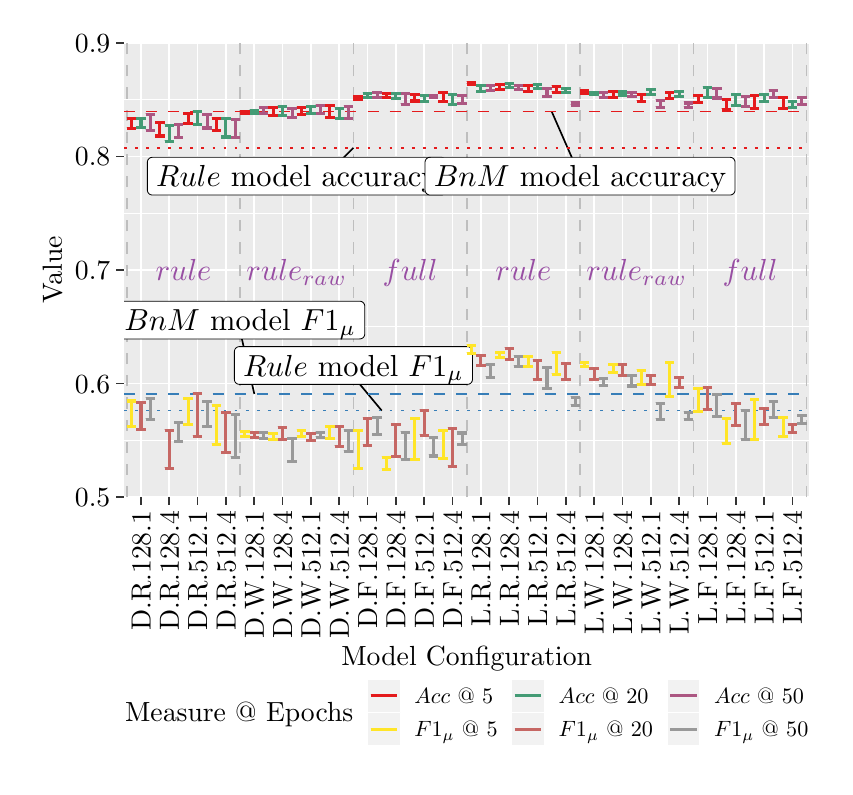
\begin{tikzpicture}[x=1pt,y=1pt]
\definecolor{fillColor}{RGB}{255,255,255}
\path[use as bounding box,fill=fillColor,fill opacity=0.00] (0,0) rectangle (288.00,266.98);
\begin{scope}
\path[clip] (  0.00,  0.00) rectangle (288.00,266.98);
\definecolor{drawColor}{RGB}{255,255,255}
\definecolor{fillColor}{RGB}{255,255,255}

\path[draw=drawColor,line width= 0.6pt,line join=round,line cap=round,fill=fillColor] (  0.00,  0.00) rectangle (288.00,266.98);
\end{scope}
\begin{scope}
\path[clip] ( 34.81, 97.36) rectangle (282.50,261.48);
\definecolor{fillColor}{gray}{0.92}

\path[fill=fillColor] ( 34.81, 97.36) rectangle (282.50,261.48);
\definecolor{drawColor}{RGB}{255,255,255}

\path[draw=drawColor,line width= 0.3pt,line join=round] ( 34.81,117.87) --
	(282.50,117.87);

\path[draw=drawColor,line width= 0.3pt,line join=round] ( 34.81,158.90) --
	(282.50,158.90);

\path[draw=drawColor,line width= 0.3pt,line join=round] ( 34.81,199.93) --
	(282.50,199.93);

\path[draw=drawColor,line width= 0.3pt,line join=round] ( 34.81,240.96) --
	(282.50,240.96);

\path[draw=drawColor,line width= 0.6pt,line join=round] ( 34.81, 97.36) --
	(282.50, 97.36);

\path[draw=drawColor,line width= 0.6pt,line join=round] ( 34.81,138.39) --
	(282.50,138.39);

\path[draw=drawColor,line width= 0.6pt,line join=round] ( 34.81,179.42) --
	(282.50,179.42);

\path[draw=drawColor,line width= 0.6pt,line join=round] ( 34.81,220.45) --
	(282.50,220.45);

\path[draw=drawColor,line width= 0.6pt,line join=round] ( 34.81,261.48) --
	(282.50,261.48);

\path[draw=drawColor,line width= 0.6pt,line join=round] ( 40.95, 97.36) --
	( 40.95,261.48);

\path[draw=drawColor,line width= 0.6pt,line join=round] ( 51.18, 97.36) --
	( 51.18,261.48);

\path[draw=drawColor,line width= 0.6pt,line join=round] ( 61.42, 97.36) --
	( 61.42,261.48);

\path[draw=drawColor,line width= 0.6pt,line join=round] ( 71.65, 97.36) --
	( 71.65,261.48);

\path[draw=drawColor,line width= 0.6pt,line join=round] ( 81.89, 97.36) --
	( 81.89,261.48);

\path[draw=drawColor,line width= 0.6pt,line join=round] ( 92.12, 97.36) --
	( 92.12,261.48);

\path[draw=drawColor,line width= 0.6pt,line join=round] (102.36, 97.36) --
	(102.36,261.48);

\path[draw=drawColor,line width= 0.6pt,line join=round] (112.59, 97.36) --
	(112.59,261.48);

\path[draw=drawColor,line width= 0.6pt,line join=round] (122.83, 97.36) --
	(122.83,261.48);

\path[draw=drawColor,line width= 0.6pt,line join=round] (133.06, 97.36) --
	(133.06,261.48);

\path[draw=drawColor,line width= 0.6pt,line join=round] (143.30, 97.36) --
	(143.30,261.48);

\path[draw=drawColor,line width= 0.6pt,line join=round] (153.54, 97.36) --
	(153.54,261.48);

\path[draw=drawColor,line width= 0.6pt,line join=round] (163.77, 97.36) --
	(163.77,261.48);

\path[draw=drawColor,line width= 0.6pt,line join=round] (174.01, 97.36) --
	(174.01,261.48);

\path[draw=drawColor,line width= 0.6pt,line join=round] (184.24, 97.36) --
	(184.24,261.48);

\path[draw=drawColor,line width= 0.6pt,line join=round] (194.48, 97.36) --
	(194.48,261.48);

\path[draw=drawColor,line width= 0.6pt,line join=round] (204.71, 97.36) --
	(204.71,261.48);

\path[draw=drawColor,line width= 0.6pt,line join=round] (214.95, 97.36) --
	(214.95,261.48);

\path[draw=drawColor,line width= 0.6pt,line join=round] (225.18, 97.36) --
	(225.18,261.48);

\path[draw=drawColor,line width= 0.6pt,line join=round] (235.42, 97.36) --
	(235.42,261.48);

\path[draw=drawColor,line width= 0.6pt,line join=round] (245.65, 97.36) --
	(245.65,261.48);

\path[draw=drawColor,line width= 0.6pt,line join=round] (255.89, 97.36) --
	(255.89,261.48);

\path[draw=drawColor,line width= 0.6pt,line join=round] (266.12, 97.36) --
	(266.12,261.48);

\path[draw=drawColor,line width= 0.6pt,line join=round] (276.36, 97.36) --
	(276.36,261.48);
\definecolor{drawColor}{RGB}{190,190,190}

\path[draw=drawColor,line width= 0.6pt,dash pattern=on 4pt off 4pt ,line join=round] ( 35.83, 97.36) -- ( 35.83,261.48);

\path[draw=drawColor,line width= 0.6pt,dash pattern=on 4pt off 4pt ,line join=round] ( 76.77, 97.36) -- ( 76.77,261.48);

\path[draw=drawColor,line width= 0.6pt,dash pattern=on 4pt off 4pt ,line join=round] (117.71, 97.36) -- (117.71,261.48);

\path[draw=drawColor,line width= 0.6pt,dash pattern=on 4pt off 4pt ,line join=round] (158.65, 97.36) -- (158.65,261.48);

\path[draw=drawColor,line width= 0.6pt,dash pattern=on 4pt off 4pt ,line join=round] (199.59, 97.36) -- (199.59,261.48);

\path[draw=drawColor,line width= 0.6pt,dash pattern=on 4pt off 4pt ,line join=round] (240.54, 97.36) -- (240.54,261.48);

\path[draw=drawColor,line width= 0.6pt,dash pattern=on 4pt off 4pt ,line join=round] (281.48, 97.36) -- (281.48,261.48);
\definecolor{drawColor}{RGB}{152,78,163}

\node[text=drawColor,anchor=base,inner sep=0pt, outer sep=0pt, scale=  1.10] at ( 56.30,175.62) {\(rule\)};

\node[text=drawColor,anchor=base,inner sep=0pt, outer sep=0pt, scale=  1.10] at ( 97.24,175.62) {\(rule_{raw}\)};

\node[text=drawColor,anchor=base,inner sep=0pt, outer sep=0pt, scale=  1.10] at (138.18,175.62) {\(full\)};

\node[text=drawColor,anchor=base,inner sep=0pt, outer sep=0pt, scale=  1.10] at (179.12,175.62) {\(rule\)};

\node[text=drawColor,anchor=base,inner sep=0pt, outer sep=0pt, scale=  1.10] at (220.06,175.62) {\(rule_{raw}\)};

\node[text=drawColor,anchor=base,inner sep=0pt, outer sep=0pt, scale=  1.10] at (261.01,175.62) {\(full\)};
\definecolor{drawColor}{RGB}{0,0,0}

\path[draw=drawColor,line width= 0.6pt,line join=round] (107.48,213.32) --
	(117.71,223.58);

\path[draw=drawColor,line width= 0.6pt,line join=round] (189.36,236.65) --
	(199.59,213.32);

\path[draw=drawColor,line width= 0.6pt,line join=round] (117.71,140.90) --
	(127.95,128.59);

\path[draw=drawColor,line width= 0.6pt,line join=round] ( 76.77,157.31) --
	( 81.89,134.65);
\definecolor{fillColor}{RGB}{255,255,255}

\path[draw=drawColor,line width= 0.3pt,line join=round,line cap=round,fill=fillColor] ( 33.55,154.50) --
	(119.99,154.50) --
	(119.92,154.51) --
	(120.21,154.52) --
	(120.49,154.58) --
	(120.76,154.68) --
	(121.01,154.82) --
	(121.24,155.01) --
	(121.43,155.23) --
	(121.59,155.47) --
	(121.70,155.74) --
	(121.77,156.02) --
	(121.79,156.31) --
	(121.79,156.31) --
	(121.79,166.32) --
	(121.79,166.32) --
	(121.77,166.61) --
	(121.70,166.90) --
	(121.59,167.16) --
	(121.43,167.41) --
	(121.24,167.63) --
	(121.01,167.81) --
	(120.76,167.96) --
	(120.49,168.06) --
	(120.21,168.12) --
	(119.99,168.13) --
	( 33.55,168.13) --
	( 33.77,168.12) --
	( 33.48,168.13) --
	( 33.19,168.09) --
	( 32.91,168.01) --
	( 32.65,167.89) --
	( 32.41,167.72) --
	( 32.20,167.52) --
	( 32.03,167.29) --
	( 31.89,167.03) --
	( 31.80,166.76) --
	( 31.75,166.47) --
	( 31.75,166.32) --
	( 31.75,156.31) --
	( 31.75,156.46) --
	( 31.75,156.17) --
	( 31.80,155.88) --
	( 31.89,155.60) --
	( 32.03,155.35) --
	( 32.20,155.11) --
	( 32.41,154.91) --
	( 32.65,154.75) --
	( 32.91,154.62) --
	( 33.19,154.54) --
	( 33.48,154.51) --
	cycle;
\end{scope}
\begin{scope}
\path[clip] ( 34.81, 97.36) rectangle (282.50,261.48);
\definecolor{drawColor}{RGB}{0,0,0}

\node[text=drawColor,anchor=base,inner sep=0pt, outer sep=0pt, scale=  1.10] at ( 76.77,157.52) {\(BnM\) model \(F1_\mu\)};
\definecolor{fillColor}{RGB}{255,255,255}

\path[draw=drawColor,line width= 0.3pt,line join=round,line cap=round,fill=fillColor] ( 76.51,138.09) --
	(158.91,138.09) --
	(158.84,138.09) --
	(159.13,138.11) --
	(159.42,138.16) --
	(159.69,138.27) --
	(159.94,138.41) --
	(160.17,138.60) --
	(160.36,138.81) --
	(160.51,139.06) --
	(160.63,139.33) --
	(160.70,139.61) --
	(160.72,139.90) --
	(160.72,139.90) --
	(160.72,149.91) --
	(160.72,149.91) --
	(160.70,150.20) --
	(160.63,150.48) --
	(160.51,150.75) --
	(160.36,151.00) --
	(160.17,151.21) --
	(159.94,151.40) --
	(159.69,151.54) --
	(159.42,151.65) --
	(159.13,151.71) --
	(158.91,151.72) --
	( 76.51,151.72) --
	( 76.73,151.71) --
	( 76.44,151.72) --
	( 76.15,151.68) --
	( 75.87,151.60) --
	( 75.61,151.48) --
	( 75.37,151.31) --
	( 75.16,151.11) --
	( 74.98,150.88) --
	( 74.85,150.62) --
	( 74.75,150.34) --
	( 74.71,150.06) --
	( 74.70,149.91) --
	( 74.70,139.90) --
	( 74.71,140.04) --
	( 74.71,139.75) --
	( 74.75,139.47) --
	( 74.85,139.19) --
	( 74.98,138.93) --
	( 75.16,138.70) --
	( 75.37,138.50) --
	( 75.61,138.33) --
	( 75.87,138.21) --
	( 76.15,138.13) --
	( 76.44,138.09) --
	cycle;
\end{scope}
\begin{scope}
\path[clip] ( 34.81, 97.36) rectangle (282.50,261.48);
\definecolor{drawColor}{RGB}{0,0,0}

\node[text=drawColor,anchor=base,inner sep=0pt, outer sep=0pt, scale=  1.10] at (117.71,141.10) {\(Rule\) model \(F1_\mu\)};
\definecolor{fillColor}{RGB}{255,255,255}

\path[draw=drawColor,line width= 0.3pt,line join=round,line cap=round,fill=fillColor] ( 45.06,206.51) --
	(149.42,206.51) --
	(149.35,206.51) --
	(149.64,206.52) --
	(149.93,206.58) --
	(150.20,206.69) --
	(150.45,206.83) --
	(150.68,207.01) --
	(150.87,207.23) --
	(151.02,207.48) --
	(151.14,207.75) --
	(151.21,208.03) --
	(151.23,208.32) --
	(151.23,208.32) --
	(151.23,218.33) --
	(151.23,218.33) --
	(151.21,218.62) --
	(151.14,218.90) --
	(151.02,219.17) --
	(150.87,219.42) --
	(150.68,219.63) --
	(150.45,219.82) --
	(150.20,219.96) --
	(149.93,220.07) --
	(149.64,220.12) --
	(149.42,220.14) --
	( 45.06,220.14) --
	( 45.28,220.12) --
	( 44.98,220.14) --
	( 44.70,220.10) --
	( 44.42,220.02) --
	( 44.15,219.89) --
	( 43.91,219.73) --
	( 43.71,219.53) --
	( 43.53,219.30) --
	( 43.40,219.04) --
	( 43.30,218.76) --
	( 43.26,218.48) --
	( 43.25,218.33) --
	( 43.25,208.32) --
	( 43.26,208.46) --
	( 43.26,208.17) --
	( 43.30,207.89) --
	( 43.40,207.61) --
	( 43.53,207.35) --
	( 43.71,207.12) --
	( 43.91,206.92) --
	( 44.15,206.75) --
	( 44.42,206.63) --
	( 44.70,206.55) --
	( 44.98,206.51) --
	cycle;
\end{scope}
\begin{scope}
\path[clip] ( 34.81, 97.36) rectangle (282.50,261.48);
\definecolor{drawColor}{RGB}{0,0,0}

\node[text=drawColor,anchor=base,inner sep=0pt, outer sep=0pt, scale=  1.10] at ( 97.24,209.52) {\(Rule\) model accuracy};
\definecolor{fillColor}{RGB}{255,255,255}

\path[draw=drawColor,line width= 0.3pt,line join=round,line cap=round,fill=fillColor] (145.40,206.51) --
	(253.79,206.51) --
	(253.72,206.51) --
	(254.01,206.52) --
	(254.29,206.58) --
	(254.57,206.69) --
	(254.82,206.83) --
	(255.04,207.01) --
	(255.24,207.23) --
	(255.39,207.48) --
	(255.51,207.75) --
	(255.58,208.03) --
	(255.60,208.32) --
	(255.60,208.32) --
	(255.60,218.33) --
	(255.60,218.33) --
	(255.58,218.62) --
	(255.51,218.90) --
	(255.39,219.17) --
	(255.24,219.42) --
	(255.04,219.63) --
	(254.82,219.82) --
	(254.57,219.96) --
	(254.29,220.07) --
	(254.01,220.12) --
	(253.79,220.14) --
	(145.40,220.14) --
	(145.61,220.12) --
	(145.32,220.14) --
	(145.03,220.10) --
	(144.76,220.02) --
	(144.49,219.89) --
	(144.25,219.73) --
	(144.04,219.53) --
	(143.87,219.30) --
	(143.73,219.04) --
	(143.64,218.76) --
	(143.60,218.48) --
	(143.59,218.33) --
	(143.59,208.32) --
	(143.60,208.46) --
	(143.60,208.17) --
	(143.64,207.89) --
	(143.73,207.61) --
	(143.87,207.35) --
	(144.04,207.12) --
	(144.25,206.92) --
	(144.49,206.75) --
	(144.76,206.63) --
	(145.03,206.55) --
	(145.32,206.51) --
	cycle;
\end{scope}
\begin{scope}
\path[clip] ( 34.81, 97.36) rectangle (282.50,261.48);
\definecolor{drawColor}{RGB}{0,0,0}

\node[text=drawColor,anchor=base,inner sep=0pt, outer sep=0pt, scale=  1.10] at (199.59,209.52) {\(BnM\) model accuracy};
\definecolor{drawColor}{RGB}{228,26,28}

\path[draw=drawColor,line width= 0.6pt,dash pattern=on 4pt off 4pt ,line join=round] ( 34.81,236.65) -- (282.50,236.65);

\path[draw=drawColor,line width= 0.6pt,dash pattern=on 1pt off 3pt ,line join=round] ( 34.81,223.58) -- (282.50,223.58);
\definecolor{drawColor}{RGB}{55,126,184}

\path[draw=drawColor,line width= 0.6pt,dash pattern=on 4pt off 4pt ,line join=round] ( 34.81,134.65) -- (282.50,134.65);

\path[draw=drawColor,line width= 0.6pt,dash pattern=on 1pt off 3pt ,line join=round] ( 34.81,128.59) -- (282.50,128.59);
\definecolor{drawColor}{RGB}{172,87,130}

\path[draw=drawColor,line width= 1.1pt,line join=round] ( 42.65,235.75) --
	( 46.06,235.75);

\path[draw=drawColor,line width= 1.1pt,line join=round] ( 44.36,235.75) --
	( 44.36,229.82);

\path[draw=drawColor,line width= 1.1pt,line join=round] ( 42.65,229.82) --
	( 46.06,229.82);

\path[draw=drawColor,line width= 1.1pt,line join=round] ( 42.65,235.75) --
	( 46.06,235.75);

\path[draw=drawColor,line width= 1.1pt,line join=round] ( 44.36,235.75) --
	( 44.36,229.82);

\path[draw=drawColor,line width= 1.1pt,line join=round] ( 42.65,229.82) --
	( 46.06,229.82);

\path[draw=drawColor,line width= 1.1pt,line join=round] ( 42.65,235.75) --
	( 46.06,235.75);

\path[draw=drawColor,line width= 1.1pt,line join=round] ( 44.36,235.75) --
	( 44.36,229.82);

\path[draw=drawColor,line width= 1.1pt,line join=round] ( 42.65,229.82) --
	( 46.06,229.82);

\path[draw=drawColor,line width= 1.1pt,line join=round] ( 42.65,235.75) --
	( 46.06,235.75);

\path[draw=drawColor,line width= 1.1pt,line join=round] ( 44.36,235.75) --
	( 44.36,229.82);

\path[draw=drawColor,line width= 1.1pt,line join=round] ( 42.65,229.82) --
	( 46.06,229.82);

\path[draw=drawColor,line width= 1.1pt,line join=round] ( 42.65,235.75) --
	( 46.06,235.75);

\path[draw=drawColor,line width= 1.1pt,line join=round] ( 44.36,235.75) --
	( 44.36,229.82);

\path[draw=drawColor,line width= 1.1pt,line join=round] ( 42.65,229.82) --
	( 46.06,229.82);

\path[draw=drawColor,line width= 1.1pt,line join=round] ( 42.65,235.75) --
	( 46.06,235.75);

\path[draw=drawColor,line width= 1.1pt,line join=round] ( 44.36,235.75) --
	( 44.36,229.82);

\path[draw=drawColor,line width= 1.1pt,line join=round] ( 42.65,229.82) --
	( 46.06,229.82);

\path[draw=drawColor,line width= 1.1pt,line join=round] ( 42.65,235.75) --
	( 46.06,235.75);

\path[draw=drawColor,line width= 1.1pt,line join=round] ( 44.36,235.75) --
	( 44.36,229.82);

\path[draw=drawColor,line width= 1.1pt,line join=round] ( 42.65,229.82) --
	( 46.06,229.82);

\path[draw=drawColor,line width= 1.1pt,line join=round] ( 42.65,235.75) --
	( 46.06,235.75);

\path[draw=drawColor,line width= 1.1pt,line join=round] ( 44.36,235.75) --
	( 44.36,229.82);

\path[draw=drawColor,line width= 1.1pt,line join=round] ( 42.65,229.82) --
	( 46.06,229.82);
\definecolor{drawColor}{RGB}{68,155,117}

\path[draw=drawColor,line width= 1.1pt,line join=round] ( 39.24,234.23) --
	( 42.65,234.23);

\path[draw=drawColor,line width= 1.1pt,line join=round] ( 40.95,234.23) --
	( 40.95,230.96);

\path[draw=drawColor,line width= 1.1pt,line join=round] ( 39.24,230.96) --
	( 42.65,230.96);

\path[draw=drawColor,line width= 1.1pt,line join=round] ( 39.24,234.23) --
	( 42.65,234.23);

\path[draw=drawColor,line width= 1.1pt,line join=round] ( 40.95,234.23) --
	( 40.95,230.96);

\path[draw=drawColor,line width= 1.1pt,line join=round] ( 39.24,230.96) --
	( 42.65,230.96);

\path[draw=drawColor,line width= 1.1pt,line join=round] ( 39.24,234.23) --
	( 42.65,234.23);

\path[draw=drawColor,line width= 1.1pt,line join=round] ( 40.95,234.23) --
	( 40.95,230.96);

\path[draw=drawColor,line width= 1.1pt,line join=round] ( 39.24,230.96) --
	( 42.65,230.96);

\path[draw=drawColor,line width= 1.1pt,line join=round] ( 39.24,234.23) --
	( 42.65,234.23);

\path[draw=drawColor,line width= 1.1pt,line join=round] ( 40.95,234.23) --
	( 40.95,230.96);

\path[draw=drawColor,line width= 1.1pt,line join=round] ( 39.24,230.96) --
	( 42.65,230.96);

\path[draw=drawColor,line width= 1.1pt,line join=round] ( 39.24,234.23) --
	( 42.65,234.23);

\path[draw=drawColor,line width= 1.1pt,line join=round] ( 40.95,234.23) --
	( 40.95,230.96);

\path[draw=drawColor,line width= 1.1pt,line join=round] ( 39.24,230.96) --
	( 42.65,230.96);

\path[draw=drawColor,line width= 1.1pt,line join=round] ( 39.24,234.23) --
	( 42.65,234.23);

\path[draw=drawColor,line width= 1.1pt,line join=round] ( 40.95,234.23) --
	( 40.95,230.96);

\path[draw=drawColor,line width= 1.1pt,line join=round] ( 39.24,230.96) --
	( 42.65,230.96);

\path[draw=drawColor,line width= 1.1pt,line join=round] ( 39.24,234.23) --
	( 42.65,234.23);

\path[draw=drawColor,line width= 1.1pt,line join=round] ( 40.95,234.23) --
	( 40.95,230.96);

\path[draw=drawColor,line width= 1.1pt,line join=round] ( 39.24,230.96) --
	( 42.65,230.96);

\path[draw=drawColor,line width= 1.1pt,line join=round] ( 39.24,234.23) --
	( 42.65,234.23);

\path[draw=drawColor,line width= 1.1pt,line join=round] ( 40.95,234.23) --
	( 40.95,230.96);

\path[draw=drawColor,line width= 1.1pt,line join=round] ( 39.24,230.96) --
	( 42.65,230.96);
\definecolor{drawColor}{RGB}{228,26,28}

\path[draw=drawColor,line width= 1.1pt,line join=round] ( 35.83,234.21) --
	( 39.24,234.21);

\path[draw=drawColor,line width= 1.1pt,line join=round] ( 37.54,234.21) --
	( 37.54,230.55);

\path[draw=drawColor,line width= 1.1pt,line join=round] ( 35.83,230.55) --
	( 39.24,230.55);

\path[draw=drawColor,line width= 1.1pt,line join=round] ( 35.83,234.21) --
	( 39.24,234.21);

\path[draw=drawColor,line width= 1.1pt,line join=round] ( 37.54,234.21) --
	( 37.54,230.55);

\path[draw=drawColor,line width= 1.1pt,line join=round] ( 35.83,230.55) --
	( 39.24,230.55);

\path[draw=drawColor,line width= 1.1pt,line join=round] ( 35.83,234.21) --
	( 39.24,234.21);

\path[draw=drawColor,line width= 1.1pt,line join=round] ( 37.54,234.21) --
	( 37.54,230.55);

\path[draw=drawColor,line width= 1.1pt,line join=round] ( 35.83,230.55) --
	( 39.24,230.55);

\path[draw=drawColor,line width= 1.1pt,line join=round] ( 35.83,234.21) --
	( 39.24,234.21);

\path[draw=drawColor,line width= 1.1pt,line join=round] ( 37.54,234.21) --
	( 37.54,230.55);

\path[draw=drawColor,line width= 1.1pt,line join=round] ( 35.83,230.55) --
	( 39.24,230.55);

\path[draw=drawColor,line width= 1.1pt,line join=round] ( 35.83,234.21) --
	( 39.24,234.21);

\path[draw=drawColor,line width= 1.1pt,line join=round] ( 37.54,234.21) --
	( 37.54,230.55);

\path[draw=drawColor,line width= 1.1pt,line join=round] ( 35.83,230.55) --
	( 39.24,230.55);

\path[draw=drawColor,line width= 1.1pt,line join=round] ( 35.83,234.21) --
	( 39.24,234.21);

\path[draw=drawColor,line width= 1.1pt,line join=round] ( 37.54,234.21) --
	( 37.54,230.55);

\path[draw=drawColor,line width= 1.1pt,line join=round] ( 35.83,230.55) --
	( 39.24,230.55);

\path[draw=drawColor,line width= 1.1pt,line join=round] ( 35.83,234.21) --
	( 39.24,234.21);

\path[draw=drawColor,line width= 1.1pt,line join=round] ( 37.54,234.21) --
	( 37.54,230.55);

\path[draw=drawColor,line width= 1.1pt,line join=round] ( 35.83,230.55) --
	( 39.24,230.55);

\path[draw=drawColor,line width= 1.1pt,line join=round] ( 35.83,234.21) --
	( 39.24,234.21);

\path[draw=drawColor,line width= 1.1pt,line join=round] ( 37.54,234.21) --
	( 37.54,230.55);

\path[draw=drawColor,line width= 1.1pt,line join=round] ( 35.83,230.55) --
	( 39.24,230.55);
\definecolor{drawColor}{RGB}{172,87,130}

\path[draw=drawColor,line width= 1.1pt,line join=round] ( 52.89,232.05) --
	( 56.30,232.05);

\path[draw=drawColor,line width= 1.1pt,line join=round] ( 54.59,232.05) --
	( 54.59,227.41);

\path[draw=drawColor,line width= 1.1pt,line join=round] ( 52.89,227.41) --
	( 56.30,227.41);

\path[draw=drawColor,line width= 1.1pt,line join=round] ( 52.89,232.05) --
	( 56.30,232.05);

\path[draw=drawColor,line width= 1.1pt,line join=round] ( 54.59,232.05) --
	( 54.59,227.41);

\path[draw=drawColor,line width= 1.1pt,line join=round] ( 52.89,227.41) --
	( 56.30,227.41);

\path[draw=drawColor,line width= 1.1pt,line join=round] ( 52.89,232.05) --
	( 56.30,232.05);

\path[draw=drawColor,line width= 1.1pt,line join=round] ( 54.59,232.05) --
	( 54.59,227.41);

\path[draw=drawColor,line width= 1.1pt,line join=round] ( 52.89,227.41) --
	( 56.30,227.41);

\path[draw=drawColor,line width= 1.1pt,line join=round] ( 52.89,232.05) --
	( 56.30,232.05);

\path[draw=drawColor,line width= 1.1pt,line join=round] ( 54.59,232.05) --
	( 54.59,227.41);

\path[draw=drawColor,line width= 1.1pt,line join=round] ( 52.89,227.41) --
	( 56.30,227.41);

\path[draw=drawColor,line width= 1.1pt,line join=round] ( 52.89,232.05) --
	( 56.30,232.05);

\path[draw=drawColor,line width= 1.1pt,line join=round] ( 54.59,232.05) --
	( 54.59,227.41);

\path[draw=drawColor,line width= 1.1pt,line join=round] ( 52.89,227.41) --
	( 56.30,227.41);

\path[draw=drawColor,line width= 1.1pt,line join=round] ( 52.89,232.05) --
	( 56.30,232.05);

\path[draw=drawColor,line width= 1.1pt,line join=round] ( 54.59,232.05) --
	( 54.59,227.41);

\path[draw=drawColor,line width= 1.1pt,line join=round] ( 52.89,227.41) --
	( 56.30,227.41);

\path[draw=drawColor,line width= 1.1pt,line join=round] ( 52.89,232.05) --
	( 56.30,232.05);

\path[draw=drawColor,line width= 1.1pt,line join=round] ( 54.59,232.05) --
	( 54.59,227.41);

\path[draw=drawColor,line width= 1.1pt,line join=round] ( 52.89,227.41) --
	( 56.30,227.41);

\path[draw=drawColor,line width= 1.1pt,line join=round] ( 52.89,232.05) --
	( 56.30,232.05);

\path[draw=drawColor,line width= 1.1pt,line join=round] ( 54.59,232.05) --
	( 54.59,227.41);

\path[draw=drawColor,line width= 1.1pt,line join=round] ( 52.89,227.41) --
	( 56.30,227.41);
\definecolor{drawColor}{RGB}{68,155,117}

\path[draw=drawColor,line width= 1.1pt,line join=round] ( 49.48,231.72) --
	( 52.89,231.72);

\path[draw=drawColor,line width= 1.1pt,line join=round] ( 51.18,231.72) --
	( 51.18,225.69);

\path[draw=drawColor,line width= 1.1pt,line join=round] ( 49.48,225.69) --
	( 52.89,225.69);

\path[draw=drawColor,line width= 1.1pt,line join=round] ( 49.48,231.72) --
	( 52.89,231.72);

\path[draw=drawColor,line width= 1.1pt,line join=round] ( 51.18,231.72) --
	( 51.18,225.69);

\path[draw=drawColor,line width= 1.1pt,line join=round] ( 49.48,225.69) --
	( 52.89,225.69);

\path[draw=drawColor,line width= 1.1pt,line join=round] ( 49.48,231.72) --
	( 52.89,231.72);

\path[draw=drawColor,line width= 1.1pt,line join=round] ( 51.18,231.72) --
	( 51.18,225.69);

\path[draw=drawColor,line width= 1.1pt,line join=round] ( 49.48,225.69) --
	( 52.89,225.69);

\path[draw=drawColor,line width= 1.1pt,line join=round] ( 49.48,231.72) --
	( 52.89,231.72);

\path[draw=drawColor,line width= 1.1pt,line join=round] ( 51.18,231.72) --
	( 51.18,225.69);

\path[draw=drawColor,line width= 1.1pt,line join=round] ( 49.48,225.69) --
	( 52.89,225.69);

\path[draw=drawColor,line width= 1.1pt,line join=round] ( 49.48,231.72) --
	( 52.89,231.72);

\path[draw=drawColor,line width= 1.1pt,line join=round] ( 51.18,231.72) --
	( 51.18,225.69);

\path[draw=drawColor,line width= 1.1pt,line join=round] ( 49.48,225.69) --
	( 52.89,225.69);

\path[draw=drawColor,line width= 1.1pt,line join=round] ( 49.48,231.72) --
	( 52.89,231.72);

\path[draw=drawColor,line width= 1.1pt,line join=round] ( 51.18,231.72) --
	( 51.18,225.69);

\path[draw=drawColor,line width= 1.1pt,line join=round] ( 49.48,225.69) --
	( 52.89,225.69);

\path[draw=drawColor,line width= 1.1pt,line join=round] ( 49.48,231.72) --
	( 52.89,231.72);

\path[draw=drawColor,line width= 1.1pt,line join=round] ( 51.18,231.72) --
	( 51.18,225.69);

\path[draw=drawColor,line width= 1.1pt,line join=round] ( 49.48,225.69) --
	( 52.89,225.69);

\path[draw=drawColor,line width= 1.1pt,line join=round] ( 49.48,231.72) --
	( 52.89,231.72);

\path[draw=drawColor,line width= 1.1pt,line join=round] ( 51.18,231.72) --
	( 51.18,225.69);

\path[draw=drawColor,line width= 1.1pt,line join=round] ( 49.48,225.69) --
	( 52.89,225.69);
\definecolor{drawColor}{RGB}{228,26,28}

\path[draw=drawColor,line width= 1.1pt,line join=round] ( 46.06,232.57) --
	( 49.48,232.57);

\path[draw=drawColor,line width= 1.1pt,line join=round] ( 47.77,232.57) --
	( 47.77,227.84);

\path[draw=drawColor,line width= 1.1pt,line join=round] ( 46.06,227.84) --
	( 49.48,227.84);

\path[draw=drawColor,line width= 1.1pt,line join=round] ( 46.06,232.57) --
	( 49.48,232.57);

\path[draw=drawColor,line width= 1.1pt,line join=round] ( 47.77,232.57) --
	( 47.77,227.84);

\path[draw=drawColor,line width= 1.1pt,line join=round] ( 46.06,227.84) --
	( 49.48,227.84);

\path[draw=drawColor,line width= 1.1pt,line join=round] ( 46.06,232.57) --
	( 49.48,232.57);

\path[draw=drawColor,line width= 1.1pt,line join=round] ( 47.77,232.57) --
	( 47.77,227.84);

\path[draw=drawColor,line width= 1.1pt,line join=round] ( 46.06,227.84) --
	( 49.48,227.84);

\path[draw=drawColor,line width= 1.1pt,line join=round] ( 46.06,232.57) --
	( 49.48,232.57);

\path[draw=drawColor,line width= 1.1pt,line join=round] ( 47.77,232.57) --
	( 47.77,227.84);

\path[draw=drawColor,line width= 1.1pt,line join=round] ( 46.06,227.84) --
	( 49.48,227.84);

\path[draw=drawColor,line width= 1.1pt,line join=round] ( 46.06,232.57) --
	( 49.48,232.57);

\path[draw=drawColor,line width= 1.1pt,line join=round] ( 47.77,232.57) --
	( 47.77,227.84);

\path[draw=drawColor,line width= 1.1pt,line join=round] ( 46.06,227.84) --
	( 49.48,227.84);

\path[draw=drawColor,line width= 1.1pt,line join=round] ( 46.06,232.57) --
	( 49.48,232.57);

\path[draw=drawColor,line width= 1.1pt,line join=round] ( 47.77,232.57) --
	( 47.77,227.84);

\path[draw=drawColor,line width= 1.1pt,line join=round] ( 46.06,227.84) --
	( 49.48,227.84);

\path[draw=drawColor,line width= 1.1pt,line join=round] ( 46.06,232.57) --
	( 49.48,232.57);

\path[draw=drawColor,line width= 1.1pt,line join=round] ( 47.77,232.57) --
	( 47.77,227.84);

\path[draw=drawColor,line width= 1.1pt,line join=round] ( 46.06,227.84) --
	( 49.48,227.84);

\path[draw=drawColor,line width= 1.1pt,line join=round] ( 46.06,232.57) --
	( 49.48,232.57);

\path[draw=drawColor,line width= 1.1pt,line join=round] ( 47.77,232.57) --
	( 47.77,227.84);

\path[draw=drawColor,line width= 1.1pt,line join=round] ( 46.06,227.84) --
	( 49.48,227.84);
\definecolor{drawColor}{RGB}{172,87,130}

\path[draw=drawColor,line width= 1.1pt,line join=round] ( 63.12,235.66) --
	( 66.54,235.66);

\path[draw=drawColor,line width= 1.1pt,line join=round] ( 64.83,235.66) --
	( 64.83,230.72);

\path[draw=drawColor,line width= 1.1pt,line join=round] ( 63.12,230.72) --
	( 66.54,230.72);

\path[draw=drawColor,line width= 1.1pt,line join=round] ( 63.12,235.66) --
	( 66.54,235.66);

\path[draw=drawColor,line width= 1.1pt,line join=round] ( 64.83,235.66) --
	( 64.83,230.72);

\path[draw=drawColor,line width= 1.1pt,line join=round] ( 63.12,230.72) --
	( 66.54,230.72);

\path[draw=drawColor,line width= 1.1pt,line join=round] ( 63.12,235.66) --
	( 66.54,235.66);

\path[draw=drawColor,line width= 1.1pt,line join=round] ( 64.83,235.66) --
	( 64.83,230.72);

\path[draw=drawColor,line width= 1.1pt,line join=round] ( 63.12,230.72) --
	( 66.54,230.72);

\path[draw=drawColor,line width= 1.1pt,line join=round] ( 63.12,235.66) --
	( 66.54,235.66);

\path[draw=drawColor,line width= 1.1pt,line join=round] ( 64.83,235.66) --
	( 64.83,230.72);

\path[draw=drawColor,line width= 1.1pt,line join=round] ( 63.12,230.72) --
	( 66.54,230.72);

\path[draw=drawColor,line width= 1.1pt,line join=round] ( 63.12,235.66) --
	( 66.54,235.66);

\path[draw=drawColor,line width= 1.1pt,line join=round] ( 64.83,235.66) --
	( 64.83,230.72);

\path[draw=drawColor,line width= 1.1pt,line join=round] ( 63.12,230.72) --
	( 66.54,230.72);

\path[draw=drawColor,line width= 1.1pt,line join=round] ( 63.12,235.66) --
	( 66.54,235.66);

\path[draw=drawColor,line width= 1.1pt,line join=round] ( 64.83,235.66) --
	( 64.83,230.72);

\path[draw=drawColor,line width= 1.1pt,line join=round] ( 63.12,230.72) --
	( 66.54,230.72);

\path[draw=drawColor,line width= 1.1pt,line join=round] ( 63.12,235.66) --
	( 66.54,235.66);

\path[draw=drawColor,line width= 1.1pt,line join=round] ( 64.83,235.66) --
	( 64.83,230.72);

\path[draw=drawColor,line width= 1.1pt,line join=round] ( 63.12,230.72) --
	( 66.54,230.72);

\path[draw=drawColor,line width= 1.1pt,line join=round] ( 63.12,235.66) --
	( 66.54,235.66);

\path[draw=drawColor,line width= 1.1pt,line join=round] ( 64.83,235.66) --
	( 64.83,230.72);

\path[draw=drawColor,line width= 1.1pt,line join=round] ( 63.12,230.72) --
	( 66.54,230.72);
\definecolor{drawColor}{RGB}{68,155,117}

\path[draw=drawColor,line width= 1.1pt,line join=round] ( 59.71,236.78) --
	( 63.12,236.78);

\path[draw=drawColor,line width= 1.1pt,line join=round] ( 61.42,236.78) --
	( 61.42,231.93);

\path[draw=drawColor,line width= 1.1pt,line join=round] ( 59.71,231.93) --
	( 63.12,231.93);

\path[draw=drawColor,line width= 1.1pt,line join=round] ( 59.71,236.78) --
	( 63.12,236.78);

\path[draw=drawColor,line width= 1.1pt,line join=round] ( 61.42,236.78) --
	( 61.42,231.93);

\path[draw=drawColor,line width= 1.1pt,line join=round] ( 59.71,231.93) --
	( 63.12,231.93);

\path[draw=drawColor,line width= 1.1pt,line join=round] ( 59.71,236.78) --
	( 63.12,236.78);

\path[draw=drawColor,line width= 1.1pt,line join=round] ( 61.42,236.78) --
	( 61.42,231.93);

\path[draw=drawColor,line width= 1.1pt,line join=round] ( 59.71,231.93) --
	( 63.12,231.93);

\path[draw=drawColor,line width= 1.1pt,line join=round] ( 59.71,236.78) --
	( 63.12,236.78);

\path[draw=drawColor,line width= 1.1pt,line join=round] ( 61.42,236.78) --
	( 61.42,231.93);

\path[draw=drawColor,line width= 1.1pt,line join=round] ( 59.71,231.93) --
	( 63.12,231.93);

\path[draw=drawColor,line width= 1.1pt,line join=round] ( 59.71,236.78) --
	( 63.12,236.78);

\path[draw=drawColor,line width= 1.1pt,line join=round] ( 61.42,236.78) --
	( 61.42,231.93);

\path[draw=drawColor,line width= 1.1pt,line join=round] ( 59.71,231.93) --
	( 63.12,231.93);

\path[draw=drawColor,line width= 1.1pt,line join=round] ( 59.71,236.78) --
	( 63.12,236.78);

\path[draw=drawColor,line width= 1.1pt,line join=round] ( 61.42,236.78) --
	( 61.42,231.93);

\path[draw=drawColor,line width= 1.1pt,line join=round] ( 59.71,231.93) --
	( 63.12,231.93);

\path[draw=drawColor,line width= 1.1pt,line join=round] ( 59.71,236.78) --
	( 63.12,236.78);

\path[draw=drawColor,line width= 1.1pt,line join=round] ( 61.42,236.78) --
	( 61.42,231.93);

\path[draw=drawColor,line width= 1.1pt,line join=round] ( 59.71,231.93) --
	( 63.12,231.93);

\path[draw=drawColor,line width= 1.1pt,line join=round] ( 59.71,236.78) --
	( 63.12,236.78);

\path[draw=drawColor,line width= 1.1pt,line join=round] ( 61.42,236.78) --
	( 61.42,231.93);

\path[draw=drawColor,line width= 1.1pt,line join=round] ( 59.71,231.93) --
	( 63.12,231.93);
\definecolor{drawColor}{RGB}{228,26,28}

\path[draw=drawColor,line width= 1.1pt,line join=round] ( 56.30,236.02) --
	( 59.71,236.02);

\path[draw=drawColor,line width= 1.1pt,line join=round] ( 58.01,236.02) --
	( 58.01,232.18);

\path[draw=drawColor,line width= 1.1pt,line join=round] ( 56.30,232.18) --
	( 59.71,232.18);

\path[draw=drawColor,line width= 1.1pt,line join=round] ( 56.30,236.02) --
	( 59.71,236.02);

\path[draw=drawColor,line width= 1.1pt,line join=round] ( 58.01,236.02) --
	( 58.01,232.18);

\path[draw=drawColor,line width= 1.1pt,line join=round] ( 56.30,232.18) --
	( 59.71,232.18);

\path[draw=drawColor,line width= 1.1pt,line join=round] ( 56.30,236.02) --
	( 59.71,236.02);

\path[draw=drawColor,line width= 1.1pt,line join=round] ( 58.01,236.02) --
	( 58.01,232.18);

\path[draw=drawColor,line width= 1.1pt,line join=round] ( 56.30,232.18) --
	( 59.71,232.18);

\path[draw=drawColor,line width= 1.1pt,line join=round] ( 56.30,236.02) --
	( 59.71,236.02);

\path[draw=drawColor,line width= 1.1pt,line join=round] ( 58.01,236.02) --
	( 58.01,232.18);

\path[draw=drawColor,line width= 1.1pt,line join=round] ( 56.30,232.18) --
	( 59.71,232.18);

\path[draw=drawColor,line width= 1.1pt,line join=round] ( 56.30,236.02) --
	( 59.71,236.02);

\path[draw=drawColor,line width= 1.1pt,line join=round] ( 58.01,236.02) --
	( 58.01,232.18);

\path[draw=drawColor,line width= 1.1pt,line join=round] ( 56.30,232.18) --
	( 59.71,232.18);

\path[draw=drawColor,line width= 1.1pt,line join=round] ( 56.30,236.02) --
	( 59.71,236.02);

\path[draw=drawColor,line width= 1.1pt,line join=round] ( 58.01,236.02) --
	( 58.01,232.18);

\path[draw=drawColor,line width= 1.1pt,line join=round] ( 56.30,232.18) --
	( 59.71,232.18);

\path[draw=drawColor,line width= 1.1pt,line join=round] ( 56.30,236.02) --
	( 59.71,236.02);

\path[draw=drawColor,line width= 1.1pt,line join=round] ( 58.01,236.02) --
	( 58.01,232.18);

\path[draw=drawColor,line width= 1.1pt,line join=round] ( 56.30,232.18) --
	( 59.71,232.18);

\path[draw=drawColor,line width= 1.1pt,line join=round] ( 56.30,236.02) --
	( 59.71,236.02);

\path[draw=drawColor,line width= 1.1pt,line join=round] ( 58.01,236.02) --
	( 58.01,232.18);

\path[draw=drawColor,line width= 1.1pt,line join=round] ( 56.30,232.18) --
	( 59.71,232.18);
\definecolor{drawColor}{RGB}{172,87,130}

\path[draw=drawColor,line width= 1.1pt,line join=round] ( 73.36,233.67) --
	( 76.77,233.67);

\path[draw=drawColor,line width= 1.1pt,line join=round] ( 75.06,233.67) --
	( 75.06,227.32);

\path[draw=drawColor,line width= 1.1pt,line join=round] ( 73.36,227.32) --
	( 76.77,227.32);

\path[draw=drawColor,line width= 1.1pt,line join=round] ( 73.36,233.67) --
	( 76.77,233.67);

\path[draw=drawColor,line width= 1.1pt,line join=round] ( 75.06,233.67) --
	( 75.06,227.32);

\path[draw=drawColor,line width= 1.1pt,line join=round] ( 73.36,227.32) --
	( 76.77,227.32);

\path[draw=drawColor,line width= 1.1pt,line join=round] ( 73.36,233.67) --
	( 76.77,233.67);

\path[draw=drawColor,line width= 1.1pt,line join=round] ( 75.06,233.67) --
	( 75.06,227.32);

\path[draw=drawColor,line width= 1.1pt,line join=round] ( 73.36,227.32) --
	( 76.77,227.32);

\path[draw=drawColor,line width= 1.1pt,line join=round] ( 73.36,233.67) --
	( 76.77,233.67);

\path[draw=drawColor,line width= 1.1pt,line join=round] ( 75.06,233.67) --
	( 75.06,227.32);

\path[draw=drawColor,line width= 1.1pt,line join=round] ( 73.36,227.32) --
	( 76.77,227.32);

\path[draw=drawColor,line width= 1.1pt,line join=round] ( 73.36,233.67) --
	( 76.77,233.67);

\path[draw=drawColor,line width= 1.1pt,line join=round] ( 75.06,233.67) --
	( 75.06,227.32);

\path[draw=drawColor,line width= 1.1pt,line join=round] ( 73.36,227.32) --
	( 76.77,227.32);

\path[draw=drawColor,line width= 1.1pt,line join=round] ( 73.36,233.67) --
	( 76.77,233.67);

\path[draw=drawColor,line width= 1.1pt,line join=round] ( 75.06,233.67) --
	( 75.06,227.32);

\path[draw=drawColor,line width= 1.1pt,line join=round] ( 73.36,227.32) --
	( 76.77,227.32);

\path[draw=drawColor,line width= 1.1pt,line join=round] ( 73.36,233.67) --
	( 76.77,233.67);

\path[draw=drawColor,line width= 1.1pt,line join=round] ( 75.06,233.67) --
	( 75.06,227.32);

\path[draw=drawColor,line width= 1.1pt,line join=round] ( 73.36,227.32) --
	( 76.77,227.32);

\path[draw=drawColor,line width= 1.1pt,line join=round] ( 73.36,233.67) --
	( 76.77,233.67);

\path[draw=drawColor,line width= 1.1pt,line join=round] ( 75.06,233.67) --
	( 75.06,227.32);

\path[draw=drawColor,line width= 1.1pt,line join=round] ( 73.36,227.32) --
	( 76.77,227.32);
\definecolor{drawColor}{RGB}{68,155,117}

\path[draw=drawColor,line width= 1.1pt,line join=round] ( 69.95,234.20) --
	( 73.36,234.20);

\path[draw=drawColor,line width= 1.1pt,line join=round] ( 71.65,234.20) --
	( 71.65,227.47);

\path[draw=drawColor,line width= 1.1pt,line join=round] ( 69.95,227.47) --
	( 73.36,227.47);

\path[draw=drawColor,line width= 1.1pt,line join=round] ( 69.95,234.20) --
	( 73.36,234.20);

\path[draw=drawColor,line width= 1.1pt,line join=round] ( 71.65,234.20) --
	( 71.65,227.47);

\path[draw=drawColor,line width= 1.1pt,line join=round] ( 69.95,227.47) --
	( 73.36,227.47);

\path[draw=drawColor,line width= 1.1pt,line join=round] ( 69.95,234.20) --
	( 73.36,234.20);

\path[draw=drawColor,line width= 1.1pt,line join=round] ( 71.65,234.20) --
	( 71.65,227.47);

\path[draw=drawColor,line width= 1.1pt,line join=round] ( 69.95,227.47) --
	( 73.36,227.47);

\path[draw=drawColor,line width= 1.1pt,line join=round] ( 69.95,234.20) --
	( 73.36,234.20);

\path[draw=drawColor,line width= 1.1pt,line join=round] ( 71.65,234.20) --
	( 71.65,227.47);

\path[draw=drawColor,line width= 1.1pt,line join=round] ( 69.95,227.47) --
	( 73.36,227.47);

\path[draw=drawColor,line width= 1.1pt,line join=round] ( 69.95,234.20) --
	( 73.36,234.20);

\path[draw=drawColor,line width= 1.1pt,line join=round] ( 71.65,234.20) --
	( 71.65,227.47);

\path[draw=drawColor,line width= 1.1pt,line join=round] ( 69.95,227.47) --
	( 73.36,227.47);

\path[draw=drawColor,line width= 1.1pt,line join=round] ( 69.95,234.20) --
	( 73.36,234.20);

\path[draw=drawColor,line width= 1.1pt,line join=round] ( 71.65,234.20) --
	( 71.65,227.47);

\path[draw=drawColor,line width= 1.1pt,line join=round] ( 69.95,227.47) --
	( 73.36,227.47);

\path[draw=drawColor,line width= 1.1pt,line join=round] ( 69.95,234.20) --
	( 73.36,234.20);

\path[draw=drawColor,line width= 1.1pt,line join=round] ( 71.65,234.20) --
	( 71.65,227.47);

\path[draw=drawColor,line width= 1.1pt,line join=round] ( 69.95,227.47) --
	( 73.36,227.47);

\path[draw=drawColor,line width= 1.1pt,line join=round] ( 69.95,234.20) --
	( 73.36,234.20);

\path[draw=drawColor,line width= 1.1pt,line join=round] ( 71.65,234.20) --
	( 71.65,227.47);

\path[draw=drawColor,line width= 1.1pt,line join=round] ( 69.95,227.47) --
	( 73.36,227.47);
\definecolor{drawColor}{RGB}{228,26,28}

\path[draw=drawColor,line width= 1.1pt,line join=round] ( 66.54,234.02) --
	( 69.95,234.02);

\path[draw=drawColor,line width= 1.1pt,line join=round] ( 68.24,234.02) --
	( 68.24,229.90);

\path[draw=drawColor,line width= 1.1pt,line join=round] ( 66.54,229.90) --
	( 69.95,229.90);

\path[draw=drawColor,line width= 1.1pt,line join=round] ( 66.54,234.02) --
	( 69.95,234.02);

\path[draw=drawColor,line width= 1.1pt,line join=round] ( 68.24,234.02) --
	( 68.24,229.90);

\path[draw=drawColor,line width= 1.1pt,line join=round] ( 66.54,229.90) --
	( 69.95,229.90);

\path[draw=drawColor,line width= 1.1pt,line join=round] ( 66.54,234.02) --
	( 69.95,234.02);

\path[draw=drawColor,line width= 1.1pt,line join=round] ( 68.24,234.02) --
	( 68.24,229.90);

\path[draw=drawColor,line width= 1.1pt,line join=round] ( 66.54,229.90) --
	( 69.95,229.90);

\path[draw=drawColor,line width= 1.1pt,line join=round] ( 66.54,234.02) --
	( 69.95,234.02);

\path[draw=drawColor,line width= 1.1pt,line join=round] ( 68.24,234.02) --
	( 68.24,229.90);

\path[draw=drawColor,line width= 1.1pt,line join=round] ( 66.54,229.90) --
	( 69.95,229.90);

\path[draw=drawColor,line width= 1.1pt,line join=round] ( 66.54,234.02) --
	( 69.95,234.02);

\path[draw=drawColor,line width= 1.1pt,line join=round] ( 68.24,234.02) --
	( 68.24,229.90);

\path[draw=drawColor,line width= 1.1pt,line join=round] ( 66.54,229.90) --
	( 69.95,229.90);

\path[draw=drawColor,line width= 1.1pt,line join=round] ( 66.54,234.02) --
	( 69.95,234.02);

\path[draw=drawColor,line width= 1.1pt,line join=round] ( 68.24,234.02) --
	( 68.24,229.90);

\path[draw=drawColor,line width= 1.1pt,line join=round] ( 66.54,229.90) --
	( 69.95,229.90);

\path[draw=drawColor,line width= 1.1pt,line join=round] ( 66.54,234.02) --
	( 69.95,234.02);

\path[draw=drawColor,line width= 1.1pt,line join=round] ( 68.24,234.02) --
	( 68.24,229.90);

\path[draw=drawColor,line width= 1.1pt,line join=round] ( 66.54,229.90) --
	( 69.95,229.90);

\path[draw=drawColor,line width= 1.1pt,line join=round] ( 66.54,234.02) --
	( 69.95,234.02);

\path[draw=drawColor,line width= 1.1pt,line join=round] ( 68.24,234.02) --
	( 68.24,229.90);

\path[draw=drawColor,line width= 1.1pt,line join=round] ( 66.54,229.90) --
	( 69.95,229.90);
\definecolor{drawColor}{RGB}{172,87,130}

\path[draw=drawColor,line width= 1.1pt,line join=round] ( 83.59,238.07) --
	( 87.01,238.07);

\path[draw=drawColor,line width= 1.1pt,line join=round] ( 85.30,238.07) --
	( 85.30,236.13);

\path[draw=drawColor,line width= 1.1pt,line join=round] ( 83.59,236.13) --
	( 87.01,236.13);

\path[draw=drawColor,line width= 1.1pt,line join=round] ( 83.59,238.07) --
	( 87.01,238.07);

\path[draw=drawColor,line width= 1.1pt,line join=round] ( 85.30,238.07) --
	( 85.30,236.13);

\path[draw=drawColor,line width= 1.1pt,line join=round] ( 83.59,236.13) --
	( 87.01,236.13);

\path[draw=drawColor,line width= 1.1pt,line join=round] ( 83.59,238.07) --
	( 87.01,238.07);

\path[draw=drawColor,line width= 1.1pt,line join=round] ( 85.30,238.07) --
	( 85.30,236.13);

\path[draw=drawColor,line width= 1.1pt,line join=round] ( 83.59,236.13) --
	( 87.01,236.13);

\path[draw=drawColor,line width= 1.1pt,line join=round] ( 83.59,238.07) --
	( 87.01,238.07);

\path[draw=drawColor,line width= 1.1pt,line join=round] ( 85.30,238.07) --
	( 85.30,236.13);

\path[draw=drawColor,line width= 1.1pt,line join=round] ( 83.59,236.13) --
	( 87.01,236.13);

\path[draw=drawColor,line width= 1.1pt,line join=round] ( 83.59,238.07) --
	( 87.01,238.07);

\path[draw=drawColor,line width= 1.1pt,line join=round] ( 85.30,238.07) --
	( 85.30,236.13);

\path[draw=drawColor,line width= 1.1pt,line join=round] ( 83.59,236.13) --
	( 87.01,236.13);

\path[draw=drawColor,line width= 1.1pt,line join=round] ( 83.59,238.07) --
	( 87.01,238.07);

\path[draw=drawColor,line width= 1.1pt,line join=round] ( 85.30,238.07) --
	( 85.30,236.13);

\path[draw=drawColor,line width= 1.1pt,line join=round] ( 83.59,236.13) --
	( 87.01,236.13);

\path[draw=drawColor,line width= 1.1pt,line join=round] ( 83.59,238.07) --
	( 87.01,238.07);

\path[draw=drawColor,line width= 1.1pt,line join=round] ( 85.30,238.07) --
	( 85.30,236.13);

\path[draw=drawColor,line width= 1.1pt,line join=round] ( 83.59,236.13) --
	( 87.01,236.13);

\path[draw=drawColor,line width= 1.1pt,line join=round] ( 83.59,238.07) --
	( 87.01,238.07);

\path[draw=drawColor,line width= 1.1pt,line join=round] ( 85.30,238.07) --
	( 85.30,236.13);

\path[draw=drawColor,line width= 1.1pt,line join=round] ( 83.59,236.13) --
	( 87.01,236.13);
\definecolor{drawColor}{RGB}{68,155,117}

\path[draw=drawColor,line width= 1.1pt,line join=round] ( 80.18,236.87) --
	( 83.59,236.87);

\path[draw=drawColor,line width= 1.1pt,line join=round] ( 81.89,236.87) --
	( 81.89,235.80);

\path[draw=drawColor,line width= 1.1pt,line join=round] ( 80.18,235.80) --
	( 83.59,235.80);

\path[draw=drawColor,line width= 1.1pt,line join=round] ( 80.18,236.87) --
	( 83.59,236.87);

\path[draw=drawColor,line width= 1.1pt,line join=round] ( 81.89,236.87) --
	( 81.89,235.80);

\path[draw=drawColor,line width= 1.1pt,line join=round] ( 80.18,235.80) --
	( 83.59,235.80);

\path[draw=drawColor,line width= 1.1pt,line join=round] ( 80.18,236.87) --
	( 83.59,236.87);

\path[draw=drawColor,line width= 1.1pt,line join=round] ( 81.89,236.87) --
	( 81.89,235.80);

\path[draw=drawColor,line width= 1.1pt,line join=round] ( 80.18,235.80) --
	( 83.59,235.80);

\path[draw=drawColor,line width= 1.1pt,line join=round] ( 80.18,236.87) --
	( 83.59,236.87);

\path[draw=drawColor,line width= 1.1pt,line join=round] ( 81.89,236.87) --
	( 81.89,235.80);

\path[draw=drawColor,line width= 1.1pt,line join=round] ( 80.18,235.80) --
	( 83.59,235.80);

\path[draw=drawColor,line width= 1.1pt,line join=round] ( 80.18,236.87) --
	( 83.59,236.87);

\path[draw=drawColor,line width= 1.1pt,line join=round] ( 81.89,236.87) --
	( 81.89,235.80);

\path[draw=drawColor,line width= 1.1pt,line join=round] ( 80.18,235.80) --
	( 83.59,235.80);

\path[draw=drawColor,line width= 1.1pt,line join=round] ( 80.18,236.87) --
	( 83.59,236.87);

\path[draw=drawColor,line width= 1.1pt,line join=round] ( 81.89,236.87) --
	( 81.89,235.80);

\path[draw=drawColor,line width= 1.1pt,line join=round] ( 80.18,235.80) --
	( 83.59,235.80);

\path[draw=drawColor,line width= 1.1pt,line join=round] ( 80.18,236.87) --
	( 83.59,236.87);

\path[draw=drawColor,line width= 1.1pt,line join=round] ( 81.89,236.87) --
	( 81.89,235.80);

\path[draw=drawColor,line width= 1.1pt,line join=round] ( 80.18,235.80) --
	( 83.59,235.80);

\path[draw=drawColor,line width= 1.1pt,line join=round] ( 80.18,236.87) --
	( 83.59,236.87);

\path[draw=drawColor,line width= 1.1pt,line join=round] ( 81.89,236.87) --
	( 81.89,235.80);

\path[draw=drawColor,line width= 1.1pt,line join=round] ( 80.18,235.80) --
	( 83.59,235.80);
\definecolor{drawColor}{RGB}{228,26,28}

\path[draw=drawColor,line width= 1.1pt,line join=round] ( 76.77,236.83) --
	( 80.18,236.83);

\path[draw=drawColor,line width= 1.1pt,line join=round] ( 78.48,236.83) --
	( 78.48,235.94);

\path[draw=drawColor,line width= 1.1pt,line join=round] ( 76.77,235.94) --
	( 80.18,235.94);

\path[draw=drawColor,line width= 1.1pt,line join=round] ( 76.77,236.83) --
	( 80.18,236.83);

\path[draw=drawColor,line width= 1.1pt,line join=round] ( 78.48,236.83) --
	( 78.48,235.94);

\path[draw=drawColor,line width= 1.1pt,line join=round] ( 76.77,235.94) --
	( 80.18,235.94);

\path[draw=drawColor,line width= 1.1pt,line join=round] ( 76.77,236.83) --
	( 80.18,236.83);

\path[draw=drawColor,line width= 1.1pt,line join=round] ( 78.48,236.83) --
	( 78.48,235.94);

\path[draw=drawColor,line width= 1.1pt,line join=round] ( 76.77,235.94) --
	( 80.18,235.94);

\path[draw=drawColor,line width= 1.1pt,line join=round] ( 76.77,236.83) --
	( 80.18,236.83);

\path[draw=drawColor,line width= 1.1pt,line join=round] ( 78.48,236.83) --
	( 78.48,235.94);

\path[draw=drawColor,line width= 1.1pt,line join=round] ( 76.77,235.94) --
	( 80.18,235.94);

\path[draw=drawColor,line width= 1.1pt,line join=round] ( 76.77,236.83) --
	( 80.18,236.83);

\path[draw=drawColor,line width= 1.1pt,line join=round] ( 78.48,236.83) --
	( 78.48,235.94);

\path[draw=drawColor,line width= 1.1pt,line join=round] ( 76.77,235.94) --
	( 80.18,235.94);

\path[draw=drawColor,line width= 1.1pt,line join=round] ( 76.77,236.83) --
	( 80.18,236.83);

\path[draw=drawColor,line width= 1.1pt,line join=round] ( 78.48,236.83) --
	( 78.48,235.94);

\path[draw=drawColor,line width= 1.1pt,line join=round] ( 76.77,235.94) --
	( 80.18,235.94);

\path[draw=drawColor,line width= 1.1pt,line join=round] ( 76.77,236.83) --
	( 80.18,236.83);

\path[draw=drawColor,line width= 1.1pt,line join=round] ( 78.48,236.83) --
	( 78.48,235.94);

\path[draw=drawColor,line width= 1.1pt,line join=round] ( 76.77,235.94) --
	( 80.18,235.94);

\path[draw=drawColor,line width= 1.1pt,line join=round] ( 76.77,236.83) --
	( 80.18,236.83);

\path[draw=drawColor,line width= 1.1pt,line join=round] ( 78.48,236.83) --
	( 78.48,235.94);

\path[draw=drawColor,line width= 1.1pt,line join=round] ( 76.77,235.94) --
	( 80.18,235.94);
\definecolor{drawColor}{RGB}{172,87,130}

\path[draw=drawColor,line width= 1.1pt,line join=round] ( 93.83,237.71) --
	( 97.24,237.71);

\path[draw=drawColor,line width= 1.1pt,line join=round] ( 95.54,237.71) --
	( 95.54,234.46);

\path[draw=drawColor,line width= 1.1pt,line join=round] ( 93.83,234.46) --
	( 97.24,234.46);

\path[draw=drawColor,line width= 1.1pt,line join=round] ( 93.83,237.71) --
	( 97.24,237.71);

\path[draw=drawColor,line width= 1.1pt,line join=round] ( 95.54,237.71) --
	( 95.54,234.46);

\path[draw=drawColor,line width= 1.1pt,line join=round] ( 93.83,234.46) --
	( 97.24,234.46);

\path[draw=drawColor,line width= 1.1pt,line join=round] ( 93.83,237.71) --
	( 97.24,237.71);

\path[draw=drawColor,line width= 1.1pt,line join=round] ( 95.54,237.71) --
	( 95.54,234.46);

\path[draw=drawColor,line width= 1.1pt,line join=round] ( 93.83,234.46) --
	( 97.24,234.46);

\path[draw=drawColor,line width= 1.1pt,line join=round] ( 93.83,237.71) --
	( 97.24,237.71);

\path[draw=drawColor,line width= 1.1pt,line join=round] ( 95.54,237.71) --
	( 95.54,234.46);

\path[draw=drawColor,line width= 1.1pt,line join=round] ( 93.83,234.46) --
	( 97.24,234.46);

\path[draw=drawColor,line width= 1.1pt,line join=round] ( 93.83,237.71) --
	( 97.24,237.71);

\path[draw=drawColor,line width= 1.1pt,line join=round] ( 95.54,237.71) --
	( 95.54,234.46);

\path[draw=drawColor,line width= 1.1pt,line join=round] ( 93.83,234.46) --
	( 97.24,234.46);

\path[draw=drawColor,line width= 1.1pt,line join=round] ( 93.83,237.71) --
	( 97.24,237.71);

\path[draw=drawColor,line width= 1.1pt,line join=round] ( 95.54,237.71) --
	( 95.54,234.46);

\path[draw=drawColor,line width= 1.1pt,line join=round] ( 93.83,234.46) --
	( 97.24,234.46);

\path[draw=drawColor,line width= 1.1pt,line join=round] ( 93.83,237.71) --
	( 97.24,237.71);

\path[draw=drawColor,line width= 1.1pt,line join=round] ( 95.54,237.71) --
	( 95.54,234.46);

\path[draw=drawColor,line width= 1.1pt,line join=round] ( 93.83,234.46) --
	( 97.24,234.46);

\path[draw=drawColor,line width= 1.1pt,line join=round] ( 93.83,237.71) --
	( 97.24,237.71);

\path[draw=drawColor,line width= 1.1pt,line join=round] ( 95.54,237.71) --
	( 95.54,234.46);

\path[draw=drawColor,line width= 1.1pt,line join=round] ( 93.83,234.46) --
	( 97.24,234.46);
\definecolor{drawColor}{RGB}{68,155,117}

\path[draw=drawColor,line width= 1.1pt,line join=round] ( 90.42,238.51) --
	( 93.83,238.51);

\path[draw=drawColor,line width= 1.1pt,line join=round] ( 92.12,238.51) --
	( 92.12,235.40);

\path[draw=drawColor,line width= 1.1pt,line join=round] ( 90.42,235.40) --
	( 93.83,235.40);

\path[draw=drawColor,line width= 1.1pt,line join=round] ( 90.42,238.51) --
	( 93.83,238.51);

\path[draw=drawColor,line width= 1.1pt,line join=round] ( 92.12,238.51) --
	( 92.12,235.40);

\path[draw=drawColor,line width= 1.1pt,line join=round] ( 90.42,235.40) --
	( 93.83,235.40);

\path[draw=drawColor,line width= 1.1pt,line join=round] ( 90.42,238.51) --
	( 93.83,238.51);

\path[draw=drawColor,line width= 1.1pt,line join=round] ( 92.12,238.51) --
	( 92.12,235.40);

\path[draw=drawColor,line width= 1.1pt,line join=round] ( 90.42,235.40) --
	( 93.83,235.40);

\path[draw=drawColor,line width= 1.1pt,line join=round] ( 90.42,238.51) --
	( 93.83,238.51);

\path[draw=drawColor,line width= 1.1pt,line join=round] ( 92.12,238.51) --
	( 92.12,235.40);

\path[draw=drawColor,line width= 1.1pt,line join=round] ( 90.42,235.40) --
	( 93.83,235.40);

\path[draw=drawColor,line width= 1.1pt,line join=round] ( 90.42,238.51) --
	( 93.83,238.51);

\path[draw=drawColor,line width= 1.1pt,line join=round] ( 92.12,238.51) --
	( 92.12,235.40);

\path[draw=drawColor,line width= 1.1pt,line join=round] ( 90.42,235.40) --
	( 93.83,235.40);

\path[draw=drawColor,line width= 1.1pt,line join=round] ( 90.42,238.51) --
	( 93.83,238.51);

\path[draw=drawColor,line width= 1.1pt,line join=round] ( 92.12,238.51) --
	( 92.12,235.40);

\path[draw=drawColor,line width= 1.1pt,line join=round] ( 90.42,235.40) --
	( 93.83,235.40);

\path[draw=drawColor,line width= 1.1pt,line join=round] ( 90.42,238.51) --
	( 93.83,238.51);

\path[draw=drawColor,line width= 1.1pt,line join=round] ( 92.12,238.51) --
	( 92.12,235.40);

\path[draw=drawColor,line width= 1.1pt,line join=round] ( 90.42,235.40) --
	( 93.83,235.40);

\path[draw=drawColor,line width= 1.1pt,line join=round] ( 90.42,238.51) --
	( 93.83,238.51);

\path[draw=drawColor,line width= 1.1pt,line join=round] ( 92.12,238.51) --
	( 92.12,235.40);

\path[draw=drawColor,line width= 1.1pt,line join=round] ( 90.42,235.40) --
	( 93.83,235.40);
\definecolor{drawColor}{RGB}{228,26,28}

\path[draw=drawColor,line width= 1.1pt,line join=round] ( 87.01,238.23) --
	( 90.42,238.23);

\path[draw=drawColor,line width= 1.1pt,line join=round] ( 88.71,238.23) --
	( 88.71,235.30);

\path[draw=drawColor,line width= 1.1pt,line join=round] ( 87.01,235.30) --
	( 90.42,235.30);

\path[draw=drawColor,line width= 1.1pt,line join=round] ( 87.01,238.23) --
	( 90.42,238.23);

\path[draw=drawColor,line width= 1.1pt,line join=round] ( 88.71,238.23) --
	( 88.71,235.30);

\path[draw=drawColor,line width= 1.1pt,line join=round] ( 87.01,235.30) --
	( 90.42,235.30);

\path[draw=drawColor,line width= 1.1pt,line join=round] ( 87.01,238.23) --
	( 90.42,238.23);

\path[draw=drawColor,line width= 1.1pt,line join=round] ( 88.71,238.23) --
	( 88.71,235.30);

\path[draw=drawColor,line width= 1.1pt,line join=round] ( 87.01,235.30) --
	( 90.42,235.30);

\path[draw=drawColor,line width= 1.1pt,line join=round] ( 87.01,238.23) --
	( 90.42,238.23);

\path[draw=drawColor,line width= 1.1pt,line join=round] ( 88.71,238.23) --
	( 88.71,235.30);

\path[draw=drawColor,line width= 1.1pt,line join=round] ( 87.01,235.30) --
	( 90.42,235.30);

\path[draw=drawColor,line width= 1.1pt,line join=round] ( 87.01,238.23) --
	( 90.42,238.23);

\path[draw=drawColor,line width= 1.1pt,line join=round] ( 88.71,238.23) --
	( 88.71,235.30);

\path[draw=drawColor,line width= 1.1pt,line join=round] ( 87.01,235.30) --
	( 90.42,235.30);

\path[draw=drawColor,line width= 1.1pt,line join=round] ( 87.01,238.23) --
	( 90.42,238.23);

\path[draw=drawColor,line width= 1.1pt,line join=round] ( 88.71,238.23) --
	( 88.71,235.30);

\path[draw=drawColor,line width= 1.1pt,line join=round] ( 87.01,235.30) --
	( 90.42,235.30);

\path[draw=drawColor,line width= 1.1pt,line join=round] ( 87.01,238.23) --
	( 90.42,238.23);

\path[draw=drawColor,line width= 1.1pt,line join=round] ( 88.71,238.23) --
	( 88.71,235.30);

\path[draw=drawColor,line width= 1.1pt,line join=round] ( 87.01,235.30) --
	( 90.42,235.30);

\path[draw=drawColor,line width= 1.1pt,line join=round] ( 87.01,238.23) --
	( 90.42,238.23);

\path[draw=drawColor,line width= 1.1pt,line join=round] ( 88.71,238.23) --
	( 88.71,235.30);

\path[draw=drawColor,line width= 1.1pt,line join=round] ( 87.01,235.30) --
	( 90.42,235.30);
\definecolor{drawColor}{RGB}{172,87,130}

\path[draw=drawColor,line width= 1.1pt,line join=round] (104.06,238.77) --
	(107.48,238.77);

\path[draw=drawColor,line width= 1.1pt,line join=round] (105.77,238.77) --
	(105.77,236.12);

\path[draw=drawColor,line width= 1.1pt,line join=round] (104.06,236.12) --
	(107.48,236.12);

\path[draw=drawColor,line width= 1.1pt,line join=round] (104.06,238.77) --
	(107.48,238.77);

\path[draw=drawColor,line width= 1.1pt,line join=round] (105.77,238.77) --
	(105.77,236.12);

\path[draw=drawColor,line width= 1.1pt,line join=round] (104.06,236.12) --
	(107.48,236.12);

\path[draw=drawColor,line width= 1.1pt,line join=round] (104.06,238.77) --
	(107.48,238.77);

\path[draw=drawColor,line width= 1.1pt,line join=round] (105.77,238.77) --
	(105.77,236.12);

\path[draw=drawColor,line width= 1.1pt,line join=round] (104.06,236.12) --
	(107.48,236.12);

\path[draw=drawColor,line width= 1.1pt,line join=round] (104.06,238.77) --
	(107.48,238.77);

\path[draw=drawColor,line width= 1.1pt,line join=round] (105.77,238.77) --
	(105.77,236.12);

\path[draw=drawColor,line width= 1.1pt,line join=round] (104.06,236.12) --
	(107.48,236.12);

\path[draw=drawColor,line width= 1.1pt,line join=round] (104.06,238.77) --
	(107.48,238.77);

\path[draw=drawColor,line width= 1.1pt,line join=round] (105.77,238.77) --
	(105.77,236.12);

\path[draw=drawColor,line width= 1.1pt,line join=round] (104.06,236.12) --
	(107.48,236.12);

\path[draw=drawColor,line width= 1.1pt,line join=round] (104.06,238.77) --
	(107.48,238.77);

\path[draw=drawColor,line width= 1.1pt,line join=round] (105.77,238.77) --
	(105.77,236.12);

\path[draw=drawColor,line width= 1.1pt,line join=round] (104.06,236.12) --
	(107.48,236.12);

\path[draw=drawColor,line width= 1.1pt,line join=round] (104.06,238.77) --
	(107.48,238.77);

\path[draw=drawColor,line width= 1.1pt,line join=round] (105.77,238.77) --
	(105.77,236.12);

\path[draw=drawColor,line width= 1.1pt,line join=round] (104.06,236.12) --
	(107.48,236.12);

\path[draw=drawColor,line width= 1.1pt,line join=round] (104.06,238.77) --
	(107.48,238.77);

\path[draw=drawColor,line width= 1.1pt,line join=round] (105.77,238.77) --
	(105.77,236.12);

\path[draw=drawColor,line width= 1.1pt,line join=round] (104.06,236.12) --
	(107.48,236.12);
\definecolor{drawColor}{RGB}{68,155,117}

\path[draw=drawColor,line width= 1.1pt,line join=round] (100.65,238.57) --
	(104.06,238.57);

\path[draw=drawColor,line width= 1.1pt,line join=round] (102.36,238.57) --
	(102.36,235.83);

\path[draw=drawColor,line width= 1.1pt,line join=round] (100.65,235.83) --
	(104.06,235.83);

\path[draw=drawColor,line width= 1.1pt,line join=round] (100.65,238.57) --
	(104.06,238.57);

\path[draw=drawColor,line width= 1.1pt,line join=round] (102.36,238.57) --
	(102.36,235.83);

\path[draw=drawColor,line width= 1.1pt,line join=round] (100.65,235.83) --
	(104.06,235.83);

\path[draw=drawColor,line width= 1.1pt,line join=round] (100.65,238.57) --
	(104.06,238.57);

\path[draw=drawColor,line width= 1.1pt,line join=round] (102.36,238.57) --
	(102.36,235.83);

\path[draw=drawColor,line width= 1.1pt,line join=round] (100.65,235.83) --
	(104.06,235.83);

\path[draw=drawColor,line width= 1.1pt,line join=round] (100.65,238.57) --
	(104.06,238.57);

\path[draw=drawColor,line width= 1.1pt,line join=round] (102.36,238.57) --
	(102.36,235.83);

\path[draw=drawColor,line width= 1.1pt,line join=round] (100.65,235.83) --
	(104.06,235.83);

\path[draw=drawColor,line width= 1.1pt,line join=round] (100.65,238.57) --
	(104.06,238.57);

\path[draw=drawColor,line width= 1.1pt,line join=round] (102.36,238.57) --
	(102.36,235.83);

\path[draw=drawColor,line width= 1.1pt,line join=round] (100.65,235.83) --
	(104.06,235.83);

\path[draw=drawColor,line width= 1.1pt,line join=round] (100.65,238.57) --
	(104.06,238.57);

\path[draw=drawColor,line width= 1.1pt,line join=round] (102.36,238.57) --
	(102.36,235.83);

\path[draw=drawColor,line width= 1.1pt,line join=round] (100.65,235.83) --
	(104.06,235.83);

\path[draw=drawColor,line width= 1.1pt,line join=round] (100.65,238.57) --
	(104.06,238.57);

\path[draw=drawColor,line width= 1.1pt,line join=round] (102.36,238.57) --
	(102.36,235.83);

\path[draw=drawColor,line width= 1.1pt,line join=round] (100.65,235.83) --
	(104.06,235.83);

\path[draw=drawColor,line width= 1.1pt,line join=round] (100.65,238.57) --
	(104.06,238.57);

\path[draw=drawColor,line width= 1.1pt,line join=round] (102.36,238.57) --
	(102.36,235.83);

\path[draw=drawColor,line width= 1.1pt,line join=round] (100.65,235.83) --
	(104.06,235.83);
\definecolor{drawColor}{RGB}{228,26,28}

\path[draw=drawColor,line width= 1.1pt,line join=round] ( 97.24,238.23) --
	(100.65,238.23);

\path[draw=drawColor,line width= 1.1pt,line join=round] ( 98.95,238.23) --
	( 98.95,235.62);

\path[draw=drawColor,line width= 1.1pt,line join=round] ( 97.24,235.62) --
	(100.65,235.62);

\path[draw=drawColor,line width= 1.1pt,line join=round] ( 97.24,238.23) --
	(100.65,238.23);

\path[draw=drawColor,line width= 1.1pt,line join=round] ( 98.95,238.23) --
	( 98.95,235.62);

\path[draw=drawColor,line width= 1.1pt,line join=round] ( 97.24,235.62) --
	(100.65,235.62);

\path[draw=drawColor,line width= 1.1pt,line join=round] ( 97.24,238.23) --
	(100.65,238.23);

\path[draw=drawColor,line width= 1.1pt,line join=round] ( 98.95,238.23) --
	( 98.95,235.62);

\path[draw=drawColor,line width= 1.1pt,line join=round] ( 97.24,235.62) --
	(100.65,235.62);

\path[draw=drawColor,line width= 1.1pt,line join=round] ( 97.24,238.23) --
	(100.65,238.23);

\path[draw=drawColor,line width= 1.1pt,line join=round] ( 98.95,238.23) --
	( 98.95,235.62);

\path[draw=drawColor,line width= 1.1pt,line join=round] ( 97.24,235.62) --
	(100.65,235.62);

\path[draw=drawColor,line width= 1.1pt,line join=round] ( 97.24,238.23) --
	(100.65,238.23);

\path[draw=drawColor,line width= 1.1pt,line join=round] ( 98.95,238.23) --
	( 98.95,235.62);

\path[draw=drawColor,line width= 1.1pt,line join=round] ( 97.24,235.62) --
	(100.65,235.62);

\path[draw=drawColor,line width= 1.1pt,line join=round] ( 97.24,238.23) --
	(100.65,238.23);

\path[draw=drawColor,line width= 1.1pt,line join=round] ( 98.95,238.23) --
	( 98.95,235.62);

\path[draw=drawColor,line width= 1.1pt,line join=round] ( 97.24,235.62) --
	(100.65,235.62);

\path[draw=drawColor,line width= 1.1pt,line join=round] ( 97.24,238.23) --
	(100.65,238.23);

\path[draw=drawColor,line width= 1.1pt,line join=round] ( 98.95,238.23) --
	( 98.95,235.62);

\path[draw=drawColor,line width= 1.1pt,line join=round] ( 97.24,235.62) --
	(100.65,235.62);

\path[draw=drawColor,line width= 1.1pt,line join=round] ( 97.24,238.23) --
	(100.65,238.23);

\path[draw=drawColor,line width= 1.1pt,line join=round] ( 98.95,238.23) --
	( 98.95,235.62);

\path[draw=drawColor,line width= 1.1pt,line join=round] ( 97.24,235.62) --
	(100.65,235.62);
\definecolor{drawColor}{RGB}{172,87,130}

\path[draw=drawColor,line width= 1.1pt,line join=round] (114.30,238.59) --
	(117.71,238.59);

\path[draw=drawColor,line width= 1.1pt,line join=round] (116.01,238.59) --
	(116.01,234.02);

\path[draw=drawColor,line width= 1.1pt,line join=round] (114.30,234.02) --
	(117.71,234.02);

\path[draw=drawColor,line width= 1.1pt,line join=round] (114.30,238.59) --
	(117.71,238.59);

\path[draw=drawColor,line width= 1.1pt,line join=round] (116.01,238.59) --
	(116.01,234.02);

\path[draw=drawColor,line width= 1.1pt,line join=round] (114.30,234.02) --
	(117.71,234.02);

\path[draw=drawColor,line width= 1.1pt,line join=round] (114.30,238.59) --
	(117.71,238.59);

\path[draw=drawColor,line width= 1.1pt,line join=round] (116.01,238.59) --
	(116.01,234.02);

\path[draw=drawColor,line width= 1.1pt,line join=round] (114.30,234.02) --
	(117.71,234.02);

\path[draw=drawColor,line width= 1.1pt,line join=round] (114.30,238.59) --
	(117.71,238.59);

\path[draw=drawColor,line width= 1.1pt,line join=round] (116.01,238.59) --
	(116.01,234.02);

\path[draw=drawColor,line width= 1.1pt,line join=round] (114.30,234.02) --
	(117.71,234.02);

\path[draw=drawColor,line width= 1.1pt,line join=round] (114.30,238.59) --
	(117.71,238.59);

\path[draw=drawColor,line width= 1.1pt,line join=round] (116.01,238.59) --
	(116.01,234.02);

\path[draw=drawColor,line width= 1.1pt,line join=round] (114.30,234.02) --
	(117.71,234.02);

\path[draw=drawColor,line width= 1.1pt,line join=round] (114.30,238.59) --
	(117.71,238.59);

\path[draw=drawColor,line width= 1.1pt,line join=round] (116.01,238.59) --
	(116.01,234.02);

\path[draw=drawColor,line width= 1.1pt,line join=round] (114.30,234.02) --
	(117.71,234.02);

\path[draw=drawColor,line width= 1.1pt,line join=round] (114.30,238.59) --
	(117.71,238.59);

\path[draw=drawColor,line width= 1.1pt,line join=round] (116.01,238.59) --
	(116.01,234.02);

\path[draw=drawColor,line width= 1.1pt,line join=round] (114.30,234.02) --
	(117.71,234.02);

\path[draw=drawColor,line width= 1.1pt,line join=round] (114.30,238.59) --
	(117.71,238.59);

\path[draw=drawColor,line width= 1.1pt,line join=round] (116.01,238.59) --
	(116.01,234.02);

\path[draw=drawColor,line width= 1.1pt,line join=round] (114.30,234.02) --
	(117.71,234.02);
\definecolor{drawColor}{RGB}{68,155,117}

\path[draw=drawColor,line width= 1.1pt,line join=round] (110.89,237.94) --
	(114.30,237.94);

\path[draw=drawColor,line width= 1.1pt,line join=round] (112.59,237.94) --
	(112.59,234.04);

\path[draw=drawColor,line width= 1.1pt,line join=round] (110.89,234.04) --
	(114.30,234.04);

\path[draw=drawColor,line width= 1.1pt,line join=round] (110.89,237.94) --
	(114.30,237.94);

\path[draw=drawColor,line width= 1.1pt,line join=round] (112.59,237.94) --
	(112.59,234.04);

\path[draw=drawColor,line width= 1.1pt,line join=round] (110.89,234.04) --
	(114.30,234.04);

\path[draw=drawColor,line width= 1.1pt,line join=round] (110.89,237.94) --
	(114.30,237.94);

\path[draw=drawColor,line width= 1.1pt,line join=round] (112.59,237.94) --
	(112.59,234.04);

\path[draw=drawColor,line width= 1.1pt,line join=round] (110.89,234.04) --
	(114.30,234.04);

\path[draw=drawColor,line width= 1.1pt,line join=round] (110.89,237.94) --
	(114.30,237.94);

\path[draw=drawColor,line width= 1.1pt,line join=round] (112.59,237.94) --
	(112.59,234.04);

\path[draw=drawColor,line width= 1.1pt,line join=round] (110.89,234.04) --
	(114.30,234.04);

\path[draw=drawColor,line width= 1.1pt,line join=round] (110.89,237.94) --
	(114.30,237.94);

\path[draw=drawColor,line width= 1.1pt,line join=round] (112.59,237.94) --
	(112.59,234.04);

\path[draw=drawColor,line width= 1.1pt,line join=round] (110.89,234.04) --
	(114.30,234.04);

\path[draw=drawColor,line width= 1.1pt,line join=round] (110.89,237.94) --
	(114.30,237.94);

\path[draw=drawColor,line width= 1.1pt,line join=round] (112.59,237.94) --
	(112.59,234.04);

\path[draw=drawColor,line width= 1.1pt,line join=round] (110.89,234.04) --
	(114.30,234.04);

\path[draw=drawColor,line width= 1.1pt,line join=round] (110.89,237.94) --
	(114.30,237.94);

\path[draw=drawColor,line width= 1.1pt,line join=round] (112.59,237.94) --
	(112.59,234.04);

\path[draw=drawColor,line width= 1.1pt,line join=round] (110.89,234.04) --
	(114.30,234.04);

\path[draw=drawColor,line width= 1.1pt,line join=round] (110.89,237.94) --
	(114.30,237.94);

\path[draw=drawColor,line width= 1.1pt,line join=round] (112.59,237.94) --
	(112.59,234.04);

\path[draw=drawColor,line width= 1.1pt,line join=round] (110.89,234.04) --
	(114.30,234.04);
\definecolor{drawColor}{RGB}{228,26,28}

\path[draw=drawColor,line width= 1.1pt,line join=round] (107.48,238.94) --
	(110.89,238.94);

\path[draw=drawColor,line width= 1.1pt,line join=round] (109.18,238.94) --
	(109.18,234.55);

\path[draw=drawColor,line width= 1.1pt,line join=round] (107.48,234.55) --
	(110.89,234.55);

\path[draw=drawColor,line width= 1.1pt,line join=round] (107.48,238.94) --
	(110.89,238.94);

\path[draw=drawColor,line width= 1.1pt,line join=round] (109.18,238.94) --
	(109.18,234.55);

\path[draw=drawColor,line width= 1.1pt,line join=round] (107.48,234.55) --
	(110.89,234.55);

\path[draw=drawColor,line width= 1.1pt,line join=round] (107.48,238.94) --
	(110.89,238.94);

\path[draw=drawColor,line width= 1.1pt,line join=round] (109.18,238.94) --
	(109.18,234.55);

\path[draw=drawColor,line width= 1.1pt,line join=round] (107.48,234.55) --
	(110.89,234.55);

\path[draw=drawColor,line width= 1.1pt,line join=round] (107.48,238.94) --
	(110.89,238.94);

\path[draw=drawColor,line width= 1.1pt,line join=round] (109.18,238.94) --
	(109.18,234.55);

\path[draw=drawColor,line width= 1.1pt,line join=round] (107.48,234.55) --
	(110.89,234.55);

\path[draw=drawColor,line width= 1.1pt,line join=round] (107.48,238.94) --
	(110.89,238.94);

\path[draw=drawColor,line width= 1.1pt,line join=round] (109.18,238.94) --
	(109.18,234.55);

\path[draw=drawColor,line width= 1.1pt,line join=round] (107.48,234.55) --
	(110.89,234.55);

\path[draw=drawColor,line width= 1.1pt,line join=round] (107.48,238.94) --
	(110.89,238.94);

\path[draw=drawColor,line width= 1.1pt,line join=round] (109.18,238.94) --
	(109.18,234.55);

\path[draw=drawColor,line width= 1.1pt,line join=round] (107.48,234.55) --
	(110.89,234.55);

\path[draw=drawColor,line width= 1.1pt,line join=round] (107.48,238.94) --
	(110.89,238.94);

\path[draw=drawColor,line width= 1.1pt,line join=round] (109.18,238.94) --
	(109.18,234.55);

\path[draw=drawColor,line width= 1.1pt,line join=round] (107.48,234.55) --
	(110.89,234.55);

\path[draw=drawColor,line width= 1.1pt,line join=round] (107.48,238.94) --
	(110.89,238.94);

\path[draw=drawColor,line width= 1.1pt,line join=round] (109.18,238.94) --
	(109.18,234.55);

\path[draw=drawColor,line width= 1.1pt,line join=round] (107.48,234.55) --
	(110.89,234.55);
\definecolor{drawColor}{RGB}{172,87,130}

\path[draw=drawColor,line width= 1.1pt,line join=round] (124.54,243.41) --
	(127.95,243.41);

\path[draw=drawColor,line width= 1.1pt,line join=round] (126.24,243.41) --
	(126.24,241.85);

\path[draw=drawColor,line width= 1.1pt,line join=round] (124.54,241.85) --
	(127.95,241.85);

\path[draw=drawColor,line width= 1.1pt,line join=round] (124.54,243.41) --
	(127.95,243.41);

\path[draw=drawColor,line width= 1.1pt,line join=round] (126.24,243.41) --
	(126.24,241.85);

\path[draw=drawColor,line width= 1.1pt,line join=round] (124.54,241.85) --
	(127.95,241.85);

\path[draw=drawColor,line width= 1.1pt,line join=round] (124.54,243.41) --
	(127.95,243.41);

\path[draw=drawColor,line width= 1.1pt,line join=round] (126.24,243.41) --
	(126.24,241.85);

\path[draw=drawColor,line width= 1.1pt,line join=round] (124.54,241.85) --
	(127.95,241.85);

\path[draw=drawColor,line width= 1.1pt,line join=round] (124.54,243.41) --
	(127.95,243.41);

\path[draw=drawColor,line width= 1.1pt,line join=round] (126.24,243.41) --
	(126.24,241.85);

\path[draw=drawColor,line width= 1.1pt,line join=round] (124.54,241.85) --
	(127.95,241.85);

\path[draw=drawColor,line width= 1.1pt,line join=round] (124.54,243.41) --
	(127.95,243.41);

\path[draw=drawColor,line width= 1.1pt,line join=round] (126.24,243.41) --
	(126.24,241.85);

\path[draw=drawColor,line width= 1.1pt,line join=round] (124.54,241.85) --
	(127.95,241.85);

\path[draw=drawColor,line width= 1.1pt,line join=round] (124.54,243.41) --
	(127.95,243.41);

\path[draw=drawColor,line width= 1.1pt,line join=round] (126.24,243.41) --
	(126.24,241.85);

\path[draw=drawColor,line width= 1.1pt,line join=round] (124.54,241.85) --
	(127.95,241.85);

\path[draw=drawColor,line width= 1.1pt,line join=round] (124.54,243.41) --
	(127.95,243.41);

\path[draw=drawColor,line width= 1.1pt,line join=round] (126.24,243.41) --
	(126.24,241.85);

\path[draw=drawColor,line width= 1.1pt,line join=round] (124.54,241.85) --
	(127.95,241.85);

\path[draw=drawColor,line width= 1.1pt,line join=round] (124.54,243.41) --
	(127.95,243.41);

\path[draw=drawColor,line width= 1.1pt,line join=round] (126.24,243.41) --
	(126.24,241.85);

\path[draw=drawColor,line width= 1.1pt,line join=round] (124.54,241.85) --
	(127.95,241.85);
\definecolor{drawColor}{RGB}{68,155,117}

\path[draw=drawColor,line width= 1.1pt,line join=round] (121.12,243.07) --
	(124.54,243.07);

\path[draw=drawColor,line width= 1.1pt,line join=round] (122.83,243.07) --
	(122.83,241.61);

\path[draw=drawColor,line width= 1.1pt,line join=round] (121.12,241.61) --
	(124.54,241.61);

\path[draw=drawColor,line width= 1.1pt,line join=round] (121.12,243.07) --
	(124.54,243.07);

\path[draw=drawColor,line width= 1.1pt,line join=round] (122.83,243.07) --
	(122.83,241.61);

\path[draw=drawColor,line width= 1.1pt,line join=round] (121.12,241.61) --
	(124.54,241.61);

\path[draw=drawColor,line width= 1.1pt,line join=round] (121.12,243.07) --
	(124.54,243.07);

\path[draw=drawColor,line width= 1.1pt,line join=round] (122.83,243.07) --
	(122.83,241.61);

\path[draw=drawColor,line width= 1.1pt,line join=round] (121.12,241.61) --
	(124.54,241.61);

\path[draw=drawColor,line width= 1.1pt,line join=round] (121.12,243.07) --
	(124.54,243.07);

\path[draw=drawColor,line width= 1.1pt,line join=round] (122.83,243.07) --
	(122.83,241.61);

\path[draw=drawColor,line width= 1.1pt,line join=round] (121.12,241.61) --
	(124.54,241.61);

\path[draw=drawColor,line width= 1.1pt,line join=round] (121.12,243.07) --
	(124.54,243.07);

\path[draw=drawColor,line width= 1.1pt,line join=round] (122.83,243.07) --
	(122.83,241.61);

\path[draw=drawColor,line width= 1.1pt,line join=round] (121.12,241.61) --
	(124.54,241.61);

\path[draw=drawColor,line width= 1.1pt,line join=round] (121.12,243.07) --
	(124.54,243.07);

\path[draw=drawColor,line width= 1.1pt,line join=round] (122.83,243.07) --
	(122.83,241.61);

\path[draw=drawColor,line width= 1.1pt,line join=round] (121.12,241.61) --
	(124.54,241.61);

\path[draw=drawColor,line width= 1.1pt,line join=round] (121.12,243.07) --
	(124.54,243.07);

\path[draw=drawColor,line width= 1.1pt,line join=round] (122.83,243.07) --
	(122.83,241.61);

\path[draw=drawColor,line width= 1.1pt,line join=round] (121.12,241.61) --
	(124.54,241.61);

\path[draw=drawColor,line width= 1.1pt,line join=round] (121.12,243.07) --
	(124.54,243.07);

\path[draw=drawColor,line width= 1.1pt,line join=round] (122.83,243.07) --
	(122.83,241.61);

\path[draw=drawColor,line width= 1.1pt,line join=round] (121.12,241.61) --
	(124.54,241.61);
\definecolor{drawColor}{RGB}{228,26,28}

\path[draw=drawColor,line width= 1.1pt,line join=round] (117.71,242.16) --
	(121.12,242.16);

\path[draw=drawColor,line width= 1.1pt,line join=round] (119.42,242.16) --
	(119.42,240.87);

\path[draw=drawColor,line width= 1.1pt,line join=round] (117.71,240.87) --
	(121.12,240.87);

\path[draw=drawColor,line width= 1.1pt,line join=round] (117.71,242.16) --
	(121.12,242.16);

\path[draw=drawColor,line width= 1.1pt,line join=round] (119.42,242.16) --
	(119.42,240.87);

\path[draw=drawColor,line width= 1.1pt,line join=round] (117.71,240.87) --
	(121.12,240.87);

\path[draw=drawColor,line width= 1.1pt,line join=round] (117.71,242.16) --
	(121.12,242.16);

\path[draw=drawColor,line width= 1.1pt,line join=round] (119.42,242.16) --
	(119.42,240.87);

\path[draw=drawColor,line width= 1.1pt,line join=round] (117.71,240.87) --
	(121.12,240.87);

\path[draw=drawColor,line width= 1.1pt,line join=round] (117.71,242.16) --
	(121.12,242.16);

\path[draw=drawColor,line width= 1.1pt,line join=round] (119.42,242.16) --
	(119.42,240.87);

\path[draw=drawColor,line width= 1.1pt,line join=round] (117.71,240.87) --
	(121.12,240.87);

\path[draw=drawColor,line width= 1.1pt,line join=round] (117.71,242.16) --
	(121.12,242.16);

\path[draw=drawColor,line width= 1.1pt,line join=round] (119.42,242.16) --
	(119.42,240.87);

\path[draw=drawColor,line width= 1.1pt,line join=round] (117.71,240.87) --
	(121.12,240.87);

\path[draw=drawColor,line width= 1.1pt,line join=round] (117.71,242.16) --
	(121.12,242.16);

\path[draw=drawColor,line width= 1.1pt,line join=round] (119.42,242.16) --
	(119.42,240.87);

\path[draw=drawColor,line width= 1.1pt,line join=round] (117.71,240.87) --
	(121.12,240.87);

\path[draw=drawColor,line width= 1.1pt,line join=round] (117.71,242.16) --
	(121.12,242.16);

\path[draw=drawColor,line width= 1.1pt,line join=round] (119.42,242.16) --
	(119.42,240.87);

\path[draw=drawColor,line width= 1.1pt,line join=round] (117.71,240.87) --
	(121.12,240.87);

\path[draw=drawColor,line width= 1.1pt,line join=round] (117.71,242.16) --
	(121.12,242.16);

\path[draw=drawColor,line width= 1.1pt,line join=round] (119.42,242.16) --
	(119.42,240.87);

\path[draw=drawColor,line width= 1.1pt,line join=round] (117.71,240.87) --
	(121.12,240.87);
\definecolor{drawColor}{RGB}{172,87,130}

\path[draw=drawColor,line width= 1.1pt,line join=round] (134.77,243.15) --
	(138.18,243.15);

\path[draw=drawColor,line width= 1.1pt,line join=round] (136.48,243.15) --
	(136.48,239.33);

\path[draw=drawColor,line width= 1.1pt,line join=round] (134.77,239.33) --
	(138.18,239.33);

\path[draw=drawColor,line width= 1.1pt,line join=round] (134.77,243.15) --
	(138.18,243.15);

\path[draw=drawColor,line width= 1.1pt,line join=round] (136.48,243.15) --
	(136.48,239.33);

\path[draw=drawColor,line width= 1.1pt,line join=round] (134.77,239.33) --
	(138.18,239.33);

\path[draw=drawColor,line width= 1.1pt,line join=round] (134.77,243.15) --
	(138.18,243.15);

\path[draw=drawColor,line width= 1.1pt,line join=round] (136.48,243.15) --
	(136.48,239.33);

\path[draw=drawColor,line width= 1.1pt,line join=round] (134.77,239.33) --
	(138.18,239.33);

\path[draw=drawColor,line width= 1.1pt,line join=round] (134.77,243.15) --
	(138.18,243.15);

\path[draw=drawColor,line width= 1.1pt,line join=round] (136.48,243.15) --
	(136.48,239.33);

\path[draw=drawColor,line width= 1.1pt,line join=round] (134.77,239.33) --
	(138.18,239.33);

\path[draw=drawColor,line width= 1.1pt,line join=round] (134.77,243.15) --
	(138.18,243.15);

\path[draw=drawColor,line width= 1.1pt,line join=round] (136.48,243.15) --
	(136.48,239.33);

\path[draw=drawColor,line width= 1.1pt,line join=round] (134.77,239.33) --
	(138.18,239.33);

\path[draw=drawColor,line width= 1.1pt,line join=round] (134.77,243.15) --
	(138.18,243.15);

\path[draw=drawColor,line width= 1.1pt,line join=round] (136.48,243.15) --
	(136.48,239.33);

\path[draw=drawColor,line width= 1.1pt,line join=round] (134.77,239.33) --
	(138.18,239.33);

\path[draw=drawColor,line width= 1.1pt,line join=round] (134.77,243.15) --
	(138.18,243.15);

\path[draw=drawColor,line width= 1.1pt,line join=round] (136.48,243.15) --
	(136.48,239.33);

\path[draw=drawColor,line width= 1.1pt,line join=round] (134.77,239.33) --
	(138.18,239.33);

\path[draw=drawColor,line width= 1.1pt,line join=round] (134.77,243.15) --
	(138.18,243.15);

\path[draw=drawColor,line width= 1.1pt,line join=round] (136.48,243.15) --
	(136.48,239.33);

\path[draw=drawColor,line width= 1.1pt,line join=round] (134.77,239.33) --
	(138.18,239.33);
\definecolor{drawColor}{RGB}{68,155,117}

\path[draw=drawColor,line width= 1.1pt,line join=round] (131.36,243.35) --
	(134.77,243.35);

\path[draw=drawColor,line width= 1.1pt,line join=round] (133.06,243.35) --
	(133.06,241.45);

\path[draw=drawColor,line width= 1.1pt,line join=round] (131.36,241.45) --
	(134.77,241.45);

\path[draw=drawColor,line width= 1.1pt,line join=round] (131.36,243.35) --
	(134.77,243.35);

\path[draw=drawColor,line width= 1.1pt,line join=round] (133.06,243.35) --
	(133.06,241.45);

\path[draw=drawColor,line width= 1.1pt,line join=round] (131.36,241.45) --
	(134.77,241.45);

\path[draw=drawColor,line width= 1.1pt,line join=round] (131.36,243.35) --
	(134.77,243.35);

\path[draw=drawColor,line width= 1.1pt,line join=round] (133.06,243.35) --
	(133.06,241.45);

\path[draw=drawColor,line width= 1.1pt,line join=round] (131.36,241.45) --
	(134.77,241.45);

\path[draw=drawColor,line width= 1.1pt,line join=round] (131.36,243.35) --
	(134.77,243.35);

\path[draw=drawColor,line width= 1.1pt,line join=round] (133.06,243.35) --
	(133.06,241.45);

\path[draw=drawColor,line width= 1.1pt,line join=round] (131.36,241.45) --
	(134.77,241.45);

\path[draw=drawColor,line width= 1.1pt,line join=round] (131.36,243.35) --
	(134.77,243.35);

\path[draw=drawColor,line width= 1.1pt,line join=round] (133.06,243.35) --
	(133.06,241.45);

\path[draw=drawColor,line width= 1.1pt,line join=round] (131.36,241.45) --
	(134.77,241.45);

\path[draw=drawColor,line width= 1.1pt,line join=round] (131.36,243.35) --
	(134.77,243.35);

\path[draw=drawColor,line width= 1.1pt,line join=round] (133.06,243.35) --
	(133.06,241.45);

\path[draw=drawColor,line width= 1.1pt,line join=round] (131.36,241.45) --
	(134.77,241.45);

\path[draw=drawColor,line width= 1.1pt,line join=round] (131.36,243.35) --
	(134.77,243.35);

\path[draw=drawColor,line width= 1.1pt,line join=round] (133.06,243.35) --
	(133.06,241.45);

\path[draw=drawColor,line width= 1.1pt,line join=round] (131.36,241.45) --
	(134.77,241.45);

\path[draw=drawColor,line width= 1.1pt,line join=round] (131.36,243.35) --
	(134.77,243.35);

\path[draw=drawColor,line width= 1.1pt,line join=round] (133.06,243.35) --
	(133.06,241.45);

\path[draw=drawColor,line width= 1.1pt,line join=round] (131.36,241.45) --
	(134.77,241.45);
\definecolor{drawColor}{RGB}{228,26,28}

\path[draw=drawColor,line width= 1.1pt,line join=round] (127.95,243.34) --
	(131.36,243.34);

\path[draw=drawColor,line width= 1.1pt,line join=round] (129.65,243.34) --
	(129.65,241.74);

\path[draw=drawColor,line width= 1.1pt,line join=round] (127.95,241.74) --
	(131.36,241.74);

\path[draw=drawColor,line width= 1.1pt,line join=round] (127.95,243.34) --
	(131.36,243.34);

\path[draw=drawColor,line width= 1.1pt,line join=round] (129.65,243.34) --
	(129.65,241.74);

\path[draw=drawColor,line width= 1.1pt,line join=round] (127.95,241.74) --
	(131.36,241.74);

\path[draw=drawColor,line width= 1.1pt,line join=round] (127.95,243.34) --
	(131.36,243.34);

\path[draw=drawColor,line width= 1.1pt,line join=round] (129.65,243.34) --
	(129.65,241.74);

\path[draw=drawColor,line width= 1.1pt,line join=round] (127.95,241.74) --
	(131.36,241.74);

\path[draw=drawColor,line width= 1.1pt,line join=round] (127.95,243.34) --
	(131.36,243.34);

\path[draw=drawColor,line width= 1.1pt,line join=round] (129.65,243.34) --
	(129.65,241.74);

\path[draw=drawColor,line width= 1.1pt,line join=round] (127.95,241.74) --
	(131.36,241.74);

\path[draw=drawColor,line width= 1.1pt,line join=round] (127.95,243.34) --
	(131.36,243.34);

\path[draw=drawColor,line width= 1.1pt,line join=round] (129.65,243.34) --
	(129.65,241.74);

\path[draw=drawColor,line width= 1.1pt,line join=round] (127.95,241.74) --
	(131.36,241.74);

\path[draw=drawColor,line width= 1.1pt,line join=round] (127.95,243.34) --
	(131.36,243.34);

\path[draw=drawColor,line width= 1.1pt,line join=round] (129.65,243.34) --
	(129.65,241.74);

\path[draw=drawColor,line width= 1.1pt,line join=round] (127.95,241.74) --
	(131.36,241.74);

\path[draw=drawColor,line width= 1.1pt,line join=round] (127.95,243.34) --
	(131.36,243.34);

\path[draw=drawColor,line width= 1.1pt,line join=round] (129.65,243.34) --
	(129.65,241.74);

\path[draw=drawColor,line width= 1.1pt,line join=round] (127.95,241.74) --
	(131.36,241.74);

\path[draw=drawColor,line width= 1.1pt,line join=round] (127.95,243.34) --
	(131.36,243.34);

\path[draw=drawColor,line width= 1.1pt,line join=round] (129.65,243.34) --
	(129.65,241.74);

\path[draw=drawColor,line width= 1.1pt,line join=round] (127.95,241.74) --
	(131.36,241.74);
\definecolor{drawColor}{RGB}{172,87,130}

\path[draw=drawColor,line width= 1.1pt,line join=round] (145.01,242.62) --
	(148.42,242.62);

\path[draw=drawColor,line width= 1.1pt,line join=round] (146.71,242.62) --
	(146.71,241.91);

\path[draw=drawColor,line width= 1.1pt,line join=round] (145.01,241.91) --
	(148.42,241.91);

\path[draw=drawColor,line width= 1.1pt,line join=round] (145.01,242.62) --
	(148.42,242.62);

\path[draw=drawColor,line width= 1.1pt,line join=round] (146.71,242.62) --
	(146.71,241.91);

\path[draw=drawColor,line width= 1.1pt,line join=round] (145.01,241.91) --
	(148.42,241.91);

\path[draw=drawColor,line width= 1.1pt,line join=round] (145.01,242.62) --
	(148.42,242.62);

\path[draw=drawColor,line width= 1.1pt,line join=round] (146.71,242.62) --
	(146.71,241.91);

\path[draw=drawColor,line width= 1.1pt,line join=round] (145.01,241.91) --
	(148.42,241.91);

\path[draw=drawColor,line width= 1.1pt,line join=round] (145.01,242.62) --
	(148.42,242.62);

\path[draw=drawColor,line width= 1.1pt,line join=round] (146.71,242.62) --
	(146.71,241.91);

\path[draw=drawColor,line width= 1.1pt,line join=round] (145.01,241.91) --
	(148.42,241.91);

\path[draw=drawColor,line width= 1.1pt,line join=round] (145.01,242.62) --
	(148.42,242.62);

\path[draw=drawColor,line width= 1.1pt,line join=round] (146.71,242.62) --
	(146.71,241.91);

\path[draw=drawColor,line width= 1.1pt,line join=round] (145.01,241.91) --
	(148.42,241.91);

\path[draw=drawColor,line width= 1.1pt,line join=round] (145.01,242.62) --
	(148.42,242.62);

\path[draw=drawColor,line width= 1.1pt,line join=round] (146.71,242.62) --
	(146.71,241.91);

\path[draw=drawColor,line width= 1.1pt,line join=round] (145.01,241.91) --
	(148.42,241.91);

\path[draw=drawColor,line width= 1.1pt,line join=round] (145.01,242.62) --
	(148.42,242.62);

\path[draw=drawColor,line width= 1.1pt,line join=round] (146.71,242.62) --
	(146.71,241.91);

\path[draw=drawColor,line width= 1.1pt,line join=round] (145.01,241.91) --
	(148.42,241.91);

\path[draw=drawColor,line width= 1.1pt,line join=round] (145.01,242.62) --
	(148.42,242.62);

\path[draw=drawColor,line width= 1.1pt,line join=round] (146.71,242.62) --
	(146.71,241.91);

\path[draw=drawColor,line width= 1.1pt,line join=round] (145.01,241.91) --
	(148.42,241.91);
\definecolor{drawColor}{RGB}{68,155,117}

\path[draw=drawColor,line width= 1.1pt,line join=round] (141.59,242.41) --
	(145.01,242.41);

\path[draw=drawColor,line width= 1.1pt,line join=round] (143.30,242.41) --
	(143.30,240.37);

\path[draw=drawColor,line width= 1.1pt,line join=round] (141.59,240.37) --
	(145.01,240.37);

\path[draw=drawColor,line width= 1.1pt,line join=round] (141.59,242.41) --
	(145.01,242.41);

\path[draw=drawColor,line width= 1.1pt,line join=round] (143.30,242.41) --
	(143.30,240.37);

\path[draw=drawColor,line width= 1.1pt,line join=round] (141.59,240.37) --
	(145.01,240.37);

\path[draw=drawColor,line width= 1.1pt,line join=round] (141.59,242.41) --
	(145.01,242.41);

\path[draw=drawColor,line width= 1.1pt,line join=round] (143.30,242.41) --
	(143.30,240.37);

\path[draw=drawColor,line width= 1.1pt,line join=round] (141.59,240.37) --
	(145.01,240.37);

\path[draw=drawColor,line width= 1.1pt,line join=round] (141.59,242.41) --
	(145.01,242.41);

\path[draw=drawColor,line width= 1.1pt,line join=round] (143.30,242.41) --
	(143.30,240.37);

\path[draw=drawColor,line width= 1.1pt,line join=round] (141.59,240.37) --
	(145.01,240.37);

\path[draw=drawColor,line width= 1.1pt,line join=round] (141.59,242.41) --
	(145.01,242.41);

\path[draw=drawColor,line width= 1.1pt,line join=round] (143.30,242.41) --
	(143.30,240.37);

\path[draw=drawColor,line width= 1.1pt,line join=round] (141.59,240.37) --
	(145.01,240.37);

\path[draw=drawColor,line width= 1.1pt,line join=round] (141.59,242.41) --
	(145.01,242.41);

\path[draw=drawColor,line width= 1.1pt,line join=round] (143.30,242.41) --
	(143.30,240.37);

\path[draw=drawColor,line width= 1.1pt,line join=round] (141.59,240.37) --
	(145.01,240.37);

\path[draw=drawColor,line width= 1.1pt,line join=round] (141.59,242.41) --
	(145.01,242.41);

\path[draw=drawColor,line width= 1.1pt,line join=round] (143.30,242.41) --
	(143.30,240.37);

\path[draw=drawColor,line width= 1.1pt,line join=round] (141.59,240.37) --
	(145.01,240.37);

\path[draw=drawColor,line width= 1.1pt,line join=round] (141.59,242.41) --
	(145.01,242.41);

\path[draw=drawColor,line width= 1.1pt,line join=round] (143.30,242.41) --
	(143.30,240.37);

\path[draw=drawColor,line width= 1.1pt,line join=round] (141.59,240.37) --
	(145.01,240.37);
\definecolor{drawColor}{RGB}{228,26,28}

\path[draw=drawColor,line width= 1.1pt,line join=round] (138.18,242.76) --
	(141.59,242.76);

\path[draw=drawColor,line width= 1.1pt,line join=round] (139.89,242.76) --
	(139.89,240.48);

\path[draw=drawColor,line width= 1.1pt,line join=round] (138.18,240.48) --
	(141.59,240.48);

\path[draw=drawColor,line width= 1.1pt,line join=round] (138.18,242.76) --
	(141.59,242.76);

\path[draw=drawColor,line width= 1.1pt,line join=round] (139.89,242.76) --
	(139.89,240.48);

\path[draw=drawColor,line width= 1.1pt,line join=round] (138.18,240.48) --
	(141.59,240.48);

\path[draw=drawColor,line width= 1.1pt,line join=round] (138.18,242.76) --
	(141.59,242.76);

\path[draw=drawColor,line width= 1.1pt,line join=round] (139.89,242.76) --
	(139.89,240.48);

\path[draw=drawColor,line width= 1.1pt,line join=round] (138.18,240.48) --
	(141.59,240.48);

\path[draw=drawColor,line width= 1.1pt,line join=round] (138.18,242.76) --
	(141.59,242.76);

\path[draw=drawColor,line width= 1.1pt,line join=round] (139.89,242.76) --
	(139.89,240.48);

\path[draw=drawColor,line width= 1.1pt,line join=round] (138.18,240.48) --
	(141.59,240.48);

\path[draw=drawColor,line width= 1.1pt,line join=round] (138.18,242.76) --
	(141.59,242.76);

\path[draw=drawColor,line width= 1.1pt,line join=round] (139.89,242.76) --
	(139.89,240.48);

\path[draw=drawColor,line width= 1.1pt,line join=round] (138.18,240.48) --
	(141.59,240.48);

\path[draw=drawColor,line width= 1.1pt,line join=round] (138.18,242.76) --
	(141.59,242.76);

\path[draw=drawColor,line width= 1.1pt,line join=round] (139.89,242.76) --
	(139.89,240.48);

\path[draw=drawColor,line width= 1.1pt,line join=round] (138.18,240.48) --
	(141.59,240.48);

\path[draw=drawColor,line width= 1.1pt,line join=round] (138.18,242.76) --
	(141.59,242.76);

\path[draw=drawColor,line width= 1.1pt,line join=round] (139.89,242.76) --
	(139.89,240.48);

\path[draw=drawColor,line width= 1.1pt,line join=round] (138.18,240.48) --
	(141.59,240.48);

\path[draw=drawColor,line width= 1.1pt,line join=round] (138.18,242.76) --
	(141.59,242.76);

\path[draw=drawColor,line width= 1.1pt,line join=round] (139.89,242.76) --
	(139.89,240.48);

\path[draw=drawColor,line width= 1.1pt,line join=round] (138.18,240.48) --
	(141.59,240.48);
\definecolor{drawColor}{RGB}{172,87,130}

\path[draw=drawColor,line width= 1.1pt,line join=round] (155.24,242.44) --
	(158.65,242.44);

\path[draw=drawColor,line width= 1.1pt,line join=round] (156.95,242.44) --
	(156.95,239.63);

\path[draw=drawColor,line width= 1.1pt,line join=round] (155.24,239.63) --
	(158.65,239.63);

\path[draw=drawColor,line width= 1.1pt,line join=round] (155.24,242.44) --
	(158.65,242.44);

\path[draw=drawColor,line width= 1.1pt,line join=round] (156.95,242.44) --
	(156.95,239.63);

\path[draw=drawColor,line width= 1.1pt,line join=round] (155.24,239.63) --
	(158.65,239.63);

\path[draw=drawColor,line width= 1.1pt,line join=round] (155.24,242.44) --
	(158.65,242.44);

\path[draw=drawColor,line width= 1.1pt,line join=round] (156.95,242.44) --
	(156.95,239.63);

\path[draw=drawColor,line width= 1.1pt,line join=round] (155.24,239.63) --
	(158.65,239.63);

\path[draw=drawColor,line width= 1.1pt,line join=round] (155.24,242.44) --
	(158.65,242.44);

\path[draw=drawColor,line width= 1.1pt,line join=round] (156.95,242.44) --
	(156.95,239.63);

\path[draw=drawColor,line width= 1.1pt,line join=round] (155.24,239.63) --
	(158.65,239.63);

\path[draw=drawColor,line width= 1.1pt,line join=round] (155.24,242.44) --
	(158.65,242.44);

\path[draw=drawColor,line width= 1.1pt,line join=round] (156.95,242.44) --
	(156.95,239.63);

\path[draw=drawColor,line width= 1.1pt,line join=round] (155.24,239.63) --
	(158.65,239.63);

\path[draw=drawColor,line width= 1.1pt,line join=round] (155.24,242.44) --
	(158.65,242.44);

\path[draw=drawColor,line width= 1.1pt,line join=round] (156.95,242.44) --
	(156.95,239.63);

\path[draw=drawColor,line width= 1.1pt,line join=round] (155.24,239.63) --
	(158.65,239.63);

\path[draw=drawColor,line width= 1.1pt,line join=round] (155.24,242.44) --
	(158.65,242.44);

\path[draw=drawColor,line width= 1.1pt,line join=round] (156.95,242.44) --
	(156.95,239.63);

\path[draw=drawColor,line width= 1.1pt,line join=round] (155.24,239.63) --
	(158.65,239.63);

\path[draw=drawColor,line width= 1.1pt,line join=round] (155.24,242.44) --
	(158.65,242.44);

\path[draw=drawColor,line width= 1.1pt,line join=round] (156.95,242.44) --
	(156.95,239.63);

\path[draw=drawColor,line width= 1.1pt,line join=round] (155.24,239.63) --
	(158.65,239.63);
\definecolor{drawColor}{RGB}{68,155,117}

\path[draw=drawColor,line width= 1.1pt,line join=round] (151.83,243.00) --
	(155.24,243.00);

\path[draw=drawColor,line width= 1.1pt,line join=round] (153.54,243.00) --
	(153.54,239.37);

\path[draw=drawColor,line width= 1.1pt,line join=round] (151.83,239.37) --
	(155.24,239.37);

\path[draw=drawColor,line width= 1.1pt,line join=round] (151.83,243.00) --
	(155.24,243.00);

\path[draw=drawColor,line width= 1.1pt,line join=round] (153.54,243.00) --
	(153.54,239.37);

\path[draw=drawColor,line width= 1.1pt,line join=round] (151.83,239.37) --
	(155.24,239.37);

\path[draw=drawColor,line width= 1.1pt,line join=round] (151.83,243.00) --
	(155.24,243.00);

\path[draw=drawColor,line width= 1.1pt,line join=round] (153.54,243.00) --
	(153.54,239.37);

\path[draw=drawColor,line width= 1.1pt,line join=round] (151.83,239.37) --
	(155.24,239.37);

\path[draw=drawColor,line width= 1.1pt,line join=round] (151.83,243.00) --
	(155.24,243.00);

\path[draw=drawColor,line width= 1.1pt,line join=round] (153.54,243.00) --
	(153.54,239.37);

\path[draw=drawColor,line width= 1.1pt,line join=round] (151.83,239.37) --
	(155.24,239.37);

\path[draw=drawColor,line width= 1.1pt,line join=round] (151.83,243.00) --
	(155.24,243.00);

\path[draw=drawColor,line width= 1.1pt,line join=round] (153.54,243.00) --
	(153.54,239.37);

\path[draw=drawColor,line width= 1.1pt,line join=round] (151.83,239.37) --
	(155.24,239.37);

\path[draw=drawColor,line width= 1.1pt,line join=round] (151.83,243.00) --
	(155.24,243.00);

\path[draw=drawColor,line width= 1.1pt,line join=round] (153.54,243.00) --
	(153.54,239.37);

\path[draw=drawColor,line width= 1.1pt,line join=round] (151.83,239.37) --
	(155.24,239.37);

\path[draw=drawColor,line width= 1.1pt,line join=round] (151.83,243.00) --
	(155.24,243.00);

\path[draw=drawColor,line width= 1.1pt,line join=round] (153.54,243.00) --
	(153.54,239.37);

\path[draw=drawColor,line width= 1.1pt,line join=round] (151.83,239.37) --
	(155.24,239.37);

\path[draw=drawColor,line width= 1.1pt,line join=round] (151.83,243.00) --
	(155.24,243.00);

\path[draw=drawColor,line width= 1.1pt,line join=round] (153.54,243.00) --
	(153.54,239.37);

\path[draw=drawColor,line width= 1.1pt,line join=round] (151.83,239.37) --
	(155.24,239.37);
\definecolor{drawColor}{RGB}{228,26,28}

\path[draw=drawColor,line width= 1.1pt,line join=round] (148.42,243.60) --
	(151.83,243.60);

\path[draw=drawColor,line width= 1.1pt,line join=round] (150.12,243.60) --
	(150.12,240.14);

\path[draw=drawColor,line width= 1.1pt,line join=round] (148.42,240.14) --
	(151.83,240.14);

\path[draw=drawColor,line width= 1.1pt,line join=round] (148.42,243.60) --
	(151.83,243.60);

\path[draw=drawColor,line width= 1.1pt,line join=round] (150.12,243.60) --
	(150.12,240.14);

\path[draw=drawColor,line width= 1.1pt,line join=round] (148.42,240.14) --
	(151.83,240.14);

\path[draw=drawColor,line width= 1.1pt,line join=round] (148.42,243.60) --
	(151.83,243.60);

\path[draw=drawColor,line width= 1.1pt,line join=round] (150.12,243.60) --
	(150.12,240.14);

\path[draw=drawColor,line width= 1.1pt,line join=round] (148.42,240.14) --
	(151.83,240.14);

\path[draw=drawColor,line width= 1.1pt,line join=round] (148.42,243.60) --
	(151.83,243.60);

\path[draw=drawColor,line width= 1.1pt,line join=round] (150.12,243.60) --
	(150.12,240.14);

\path[draw=drawColor,line width= 1.1pt,line join=round] (148.42,240.14) --
	(151.83,240.14);

\path[draw=drawColor,line width= 1.1pt,line join=round] (148.42,243.60) --
	(151.83,243.60);

\path[draw=drawColor,line width= 1.1pt,line join=round] (150.12,243.60) --
	(150.12,240.14);

\path[draw=drawColor,line width= 1.1pt,line join=round] (148.42,240.14) --
	(151.83,240.14);

\path[draw=drawColor,line width= 1.1pt,line join=round] (148.42,243.60) --
	(151.83,243.60);

\path[draw=drawColor,line width= 1.1pt,line join=round] (150.12,243.60) --
	(150.12,240.14);

\path[draw=drawColor,line width= 1.1pt,line join=round] (148.42,240.14) --
	(151.83,240.14);

\path[draw=drawColor,line width= 1.1pt,line join=round] (148.42,243.60) --
	(151.83,243.60);

\path[draw=drawColor,line width= 1.1pt,line join=round] (150.12,243.60) --
	(150.12,240.14);

\path[draw=drawColor,line width= 1.1pt,line join=round] (148.42,240.14) --
	(151.83,240.14);

\path[draw=drawColor,line width= 1.1pt,line join=round] (148.42,243.60) --
	(151.83,243.60);

\path[draw=drawColor,line width= 1.1pt,line join=round] (150.12,243.60) --
	(150.12,240.14);

\path[draw=drawColor,line width= 1.1pt,line join=round] (148.42,240.14) --
	(151.83,240.14);
\definecolor{drawColor}{RGB}{172,87,130}

\path[draw=drawColor,line width= 1.1pt,line join=round] (165.48,246.07) --
	(168.89,246.07);

\path[draw=drawColor,line width= 1.1pt,line join=round] (167.18,246.07) --
	(167.18,244.27);

\path[draw=drawColor,line width= 1.1pt,line join=round] (165.48,244.27) --
	(168.89,244.27);

\path[draw=drawColor,line width= 1.1pt,line join=round] (165.48,246.07) --
	(168.89,246.07);

\path[draw=drawColor,line width= 1.1pt,line join=round] (167.18,246.07) --
	(167.18,244.27);

\path[draw=drawColor,line width= 1.1pt,line join=round] (165.48,244.27) --
	(168.89,244.27);

\path[draw=drawColor,line width= 1.1pt,line join=round] (165.48,246.07) --
	(168.89,246.07);

\path[draw=drawColor,line width= 1.1pt,line join=round] (167.18,246.07) --
	(167.18,244.27);

\path[draw=drawColor,line width= 1.1pt,line join=round] (165.48,244.27) --
	(168.89,244.27);

\path[draw=drawColor,line width= 1.1pt,line join=round] (165.48,246.07) --
	(168.89,246.07);

\path[draw=drawColor,line width= 1.1pt,line join=round] (167.18,246.07) --
	(167.18,244.27);

\path[draw=drawColor,line width= 1.1pt,line join=round] (165.48,244.27) --
	(168.89,244.27);

\path[draw=drawColor,line width= 1.1pt,line join=round] (165.48,246.07) --
	(168.89,246.07);

\path[draw=drawColor,line width= 1.1pt,line join=round] (167.18,246.07) --
	(167.18,244.27);

\path[draw=drawColor,line width= 1.1pt,line join=round] (165.48,244.27) --
	(168.89,244.27);

\path[draw=drawColor,line width= 1.1pt,line join=round] (165.48,246.07) --
	(168.89,246.07);

\path[draw=drawColor,line width= 1.1pt,line join=round] (167.18,246.07) --
	(167.18,244.27);

\path[draw=drawColor,line width= 1.1pt,line join=round] (165.48,244.27) --
	(168.89,244.27);

\path[draw=drawColor,line width= 1.1pt,line join=round] (165.48,246.07) --
	(168.89,246.07);

\path[draw=drawColor,line width= 1.1pt,line join=round] (167.18,246.07) --
	(167.18,244.27);

\path[draw=drawColor,line width= 1.1pt,line join=round] (165.48,244.27) --
	(168.89,244.27);

\path[draw=drawColor,line width= 1.1pt,line join=round] (165.48,246.07) --
	(168.89,246.07);

\path[draw=drawColor,line width= 1.1pt,line join=round] (167.18,246.07) --
	(167.18,244.27);

\path[draw=drawColor,line width= 1.1pt,line join=round] (165.48,244.27) --
	(168.89,244.27);
\definecolor{drawColor}{RGB}{68,155,117}

\path[draw=drawColor,line width= 1.1pt,line join=round] (162.06,246.17) --
	(165.48,246.17);

\path[draw=drawColor,line width= 1.1pt,line join=round] (163.77,246.17) --
	(163.77,243.90);

\path[draw=drawColor,line width= 1.1pt,line join=round] (162.06,243.90) --
	(165.48,243.90);

\path[draw=drawColor,line width= 1.1pt,line join=round] (162.06,246.17) --
	(165.48,246.17);

\path[draw=drawColor,line width= 1.1pt,line join=round] (163.77,246.17) --
	(163.77,243.90);

\path[draw=drawColor,line width= 1.1pt,line join=round] (162.06,243.90) --
	(165.48,243.90);

\path[draw=drawColor,line width= 1.1pt,line join=round] (162.06,246.17) --
	(165.48,246.17);

\path[draw=drawColor,line width= 1.1pt,line join=round] (163.77,246.17) --
	(163.77,243.90);

\path[draw=drawColor,line width= 1.1pt,line join=round] (162.06,243.90) --
	(165.48,243.90);

\path[draw=drawColor,line width= 1.1pt,line join=round] (162.06,246.17) --
	(165.48,246.17);

\path[draw=drawColor,line width= 1.1pt,line join=round] (163.77,246.17) --
	(163.77,243.90);

\path[draw=drawColor,line width= 1.1pt,line join=round] (162.06,243.90) --
	(165.48,243.90);

\path[draw=drawColor,line width= 1.1pt,line join=round] (162.06,246.17) --
	(165.48,246.17);

\path[draw=drawColor,line width= 1.1pt,line join=round] (163.77,246.17) --
	(163.77,243.90);

\path[draw=drawColor,line width= 1.1pt,line join=round] (162.06,243.90) --
	(165.48,243.90);

\path[draw=drawColor,line width= 1.1pt,line join=round] (162.06,246.17) --
	(165.48,246.17);

\path[draw=drawColor,line width= 1.1pt,line join=round] (163.77,246.17) --
	(163.77,243.90);

\path[draw=drawColor,line width= 1.1pt,line join=round] (162.06,243.90) --
	(165.48,243.90);

\path[draw=drawColor,line width= 1.1pt,line join=round] (162.06,246.17) --
	(165.48,246.17);

\path[draw=drawColor,line width= 1.1pt,line join=round] (163.77,246.17) --
	(163.77,243.90);

\path[draw=drawColor,line width= 1.1pt,line join=round] (162.06,243.90) --
	(165.48,243.90);

\path[draw=drawColor,line width= 1.1pt,line join=round] (162.06,246.17) --
	(165.48,246.17);

\path[draw=drawColor,line width= 1.1pt,line join=round] (163.77,246.17) --
	(163.77,243.90);

\path[draw=drawColor,line width= 1.1pt,line join=round] (162.06,243.90) --
	(165.48,243.90);
\definecolor{drawColor}{RGB}{228,26,28}

\path[draw=drawColor,line width= 1.1pt,line join=round] (158.65,247.33) --
	(162.06,247.33);

\path[draw=drawColor,line width= 1.1pt,line join=round] (160.36,247.33) --
	(160.36,246.49);

\path[draw=drawColor,line width= 1.1pt,line join=round] (158.65,246.49) --
	(162.06,246.49);

\path[draw=drawColor,line width= 1.1pt,line join=round] (158.65,247.33) --
	(162.06,247.33);

\path[draw=drawColor,line width= 1.1pt,line join=round] (160.36,247.33) --
	(160.36,246.49);

\path[draw=drawColor,line width= 1.1pt,line join=round] (158.65,246.49) --
	(162.06,246.49);

\path[draw=drawColor,line width= 1.1pt,line join=round] (158.65,247.33) --
	(162.06,247.33);

\path[draw=drawColor,line width= 1.1pt,line join=round] (160.36,247.33) --
	(160.36,246.49);

\path[draw=drawColor,line width= 1.1pt,line join=round] (158.65,246.49) --
	(162.06,246.49);

\path[draw=drawColor,line width= 1.1pt,line join=round] (158.65,247.33) --
	(162.06,247.33);

\path[draw=drawColor,line width= 1.1pt,line join=round] (160.36,247.33) --
	(160.36,246.49);

\path[draw=drawColor,line width= 1.1pt,line join=round] (158.65,246.49) --
	(162.06,246.49);

\path[draw=drawColor,line width= 1.1pt,line join=round] (158.65,247.33) --
	(162.06,247.33);

\path[draw=drawColor,line width= 1.1pt,line join=round] (160.36,247.33) --
	(160.36,246.49);

\path[draw=drawColor,line width= 1.1pt,line join=round] (158.65,246.49) --
	(162.06,246.49);

\path[draw=drawColor,line width= 1.1pt,line join=round] (158.65,247.33) --
	(162.06,247.33);

\path[draw=drawColor,line width= 1.1pt,line join=round] (160.36,247.33) --
	(160.36,246.49);

\path[draw=drawColor,line width= 1.1pt,line join=round] (158.65,246.49) --
	(162.06,246.49);

\path[draw=drawColor,line width= 1.1pt,line join=round] (158.65,247.33) --
	(162.06,247.33);

\path[draw=drawColor,line width= 1.1pt,line join=round] (160.36,247.33) --
	(160.36,246.49);

\path[draw=drawColor,line width= 1.1pt,line join=round] (158.65,246.49) --
	(162.06,246.49);

\path[draw=drawColor,line width= 1.1pt,line join=round] (158.65,247.33) --
	(162.06,247.33);

\path[draw=drawColor,line width= 1.1pt,line join=round] (160.36,247.33) --
	(160.36,246.49);

\path[draw=drawColor,line width= 1.1pt,line join=round] (158.65,246.49) --
	(162.06,246.49);
\definecolor{drawColor}{RGB}{172,87,130}

\path[draw=drawColor,line width= 1.1pt,line join=round] (175.71,245.91) --
	(179.12,245.91);

\path[draw=drawColor,line width= 1.1pt,line join=round] (177.42,245.91) --
	(177.42,244.80);

\path[draw=drawColor,line width= 1.1pt,line join=round] (175.71,244.80) --
	(179.12,244.80);

\path[draw=drawColor,line width= 1.1pt,line join=round] (175.71,245.91) --
	(179.12,245.91);

\path[draw=drawColor,line width= 1.1pt,line join=round] (177.42,245.91) --
	(177.42,244.80);

\path[draw=drawColor,line width= 1.1pt,line join=round] (175.71,244.80) --
	(179.12,244.80);

\path[draw=drawColor,line width= 1.1pt,line join=round] (175.71,245.91) --
	(179.12,245.91);

\path[draw=drawColor,line width= 1.1pt,line join=round] (177.42,245.91) --
	(177.42,244.80);

\path[draw=drawColor,line width= 1.1pt,line join=round] (175.71,244.80) --
	(179.12,244.80);

\path[draw=drawColor,line width= 1.1pt,line join=round] (175.71,245.91) --
	(179.12,245.91);

\path[draw=drawColor,line width= 1.1pt,line join=round] (177.42,245.91) --
	(177.42,244.80);

\path[draw=drawColor,line width= 1.1pt,line join=round] (175.71,244.80) --
	(179.12,244.80);

\path[draw=drawColor,line width= 1.1pt,line join=round] (175.71,245.91) --
	(179.12,245.91);

\path[draw=drawColor,line width= 1.1pt,line join=round] (177.42,245.91) --
	(177.42,244.80);

\path[draw=drawColor,line width= 1.1pt,line join=round] (175.71,244.80) --
	(179.12,244.80);

\path[draw=drawColor,line width= 1.1pt,line join=round] (175.71,245.91) --
	(179.12,245.91);

\path[draw=drawColor,line width= 1.1pt,line join=round] (177.42,245.91) --
	(177.42,244.80);

\path[draw=drawColor,line width= 1.1pt,line join=round] (175.71,244.80) --
	(179.12,244.80);

\path[draw=drawColor,line width= 1.1pt,line join=round] (175.71,245.91) --
	(179.12,245.91);

\path[draw=drawColor,line width= 1.1pt,line join=round] (177.42,245.91) --
	(177.42,244.80);

\path[draw=drawColor,line width= 1.1pt,line join=round] (175.71,244.80) --
	(179.12,244.80);

\path[draw=drawColor,line width= 1.1pt,line join=round] (175.71,245.91) --
	(179.12,245.91);

\path[draw=drawColor,line width= 1.1pt,line join=round] (177.42,245.91) --
	(177.42,244.80);

\path[draw=drawColor,line width= 1.1pt,line join=round] (175.71,244.80) --
	(179.12,244.80);
\definecolor{drawColor}{RGB}{68,155,117}

\path[draw=drawColor,line width= 1.1pt,line join=round] (172.30,246.94) --
	(175.71,246.94);

\path[draw=drawColor,line width= 1.1pt,line join=round] (174.01,246.94) --
	(174.01,245.43);

\path[draw=drawColor,line width= 1.1pt,line join=round] (172.30,245.43) --
	(175.71,245.43);

\path[draw=drawColor,line width= 1.1pt,line join=round] (172.30,246.94) --
	(175.71,246.94);

\path[draw=drawColor,line width= 1.1pt,line join=round] (174.01,246.94) --
	(174.01,245.43);

\path[draw=drawColor,line width= 1.1pt,line join=round] (172.30,245.43) --
	(175.71,245.43);

\path[draw=drawColor,line width= 1.1pt,line join=round] (172.30,246.94) --
	(175.71,246.94);

\path[draw=drawColor,line width= 1.1pt,line join=round] (174.01,246.94) --
	(174.01,245.43);

\path[draw=drawColor,line width= 1.1pt,line join=round] (172.30,245.43) --
	(175.71,245.43);

\path[draw=drawColor,line width= 1.1pt,line join=round] (172.30,246.94) --
	(175.71,246.94);

\path[draw=drawColor,line width= 1.1pt,line join=round] (174.01,246.94) --
	(174.01,245.43);

\path[draw=drawColor,line width= 1.1pt,line join=round] (172.30,245.43) --
	(175.71,245.43);

\path[draw=drawColor,line width= 1.1pt,line join=round] (172.30,246.94) --
	(175.71,246.94);

\path[draw=drawColor,line width= 1.1pt,line join=round] (174.01,246.94) --
	(174.01,245.43);

\path[draw=drawColor,line width= 1.1pt,line join=round] (172.30,245.43) --
	(175.71,245.43);

\path[draw=drawColor,line width= 1.1pt,line join=round] (172.30,246.94) --
	(175.71,246.94);

\path[draw=drawColor,line width= 1.1pt,line join=round] (174.01,246.94) --
	(174.01,245.43);

\path[draw=drawColor,line width= 1.1pt,line join=round] (172.30,245.43) --
	(175.71,245.43);

\path[draw=drawColor,line width= 1.1pt,line join=round] (172.30,246.94) --
	(175.71,246.94);

\path[draw=drawColor,line width= 1.1pt,line join=round] (174.01,246.94) --
	(174.01,245.43);

\path[draw=drawColor,line width= 1.1pt,line join=round] (172.30,245.43) --
	(175.71,245.43);

\path[draw=drawColor,line width= 1.1pt,line join=round] (172.30,246.94) --
	(175.71,246.94);

\path[draw=drawColor,line width= 1.1pt,line join=round] (174.01,246.94) --
	(174.01,245.43);

\path[draw=drawColor,line width= 1.1pt,line join=round] (172.30,245.43) --
	(175.71,245.43);
\definecolor{drawColor}{RGB}{228,26,28}

\path[draw=drawColor,line width= 1.1pt,line join=round] (168.89,246.38) --
	(172.30,246.38);

\path[draw=drawColor,line width= 1.1pt,line join=round] (170.59,246.38) --
	(170.59,244.53);

\path[draw=drawColor,line width= 1.1pt,line join=round] (168.89,244.53) --
	(172.30,244.53);

\path[draw=drawColor,line width= 1.1pt,line join=round] (168.89,246.38) --
	(172.30,246.38);

\path[draw=drawColor,line width= 1.1pt,line join=round] (170.59,246.38) --
	(170.59,244.53);

\path[draw=drawColor,line width= 1.1pt,line join=round] (168.89,244.53) --
	(172.30,244.53);

\path[draw=drawColor,line width= 1.1pt,line join=round] (168.89,246.38) --
	(172.30,246.38);

\path[draw=drawColor,line width= 1.1pt,line join=round] (170.59,246.38) --
	(170.59,244.53);

\path[draw=drawColor,line width= 1.1pt,line join=round] (168.89,244.53) --
	(172.30,244.53);

\path[draw=drawColor,line width= 1.1pt,line join=round] (168.89,246.38) --
	(172.30,246.38);

\path[draw=drawColor,line width= 1.1pt,line join=round] (170.59,246.38) --
	(170.59,244.53);

\path[draw=drawColor,line width= 1.1pt,line join=round] (168.89,244.53) --
	(172.30,244.53);

\path[draw=drawColor,line width= 1.1pt,line join=round] (168.89,246.38) --
	(172.30,246.38);

\path[draw=drawColor,line width= 1.1pt,line join=round] (170.59,246.38) --
	(170.59,244.53);

\path[draw=drawColor,line width= 1.1pt,line join=round] (168.89,244.53) --
	(172.30,244.53);

\path[draw=drawColor,line width= 1.1pt,line join=round] (168.89,246.38) --
	(172.30,246.38);

\path[draw=drawColor,line width= 1.1pt,line join=round] (170.59,246.38) --
	(170.59,244.53);

\path[draw=drawColor,line width= 1.1pt,line join=round] (168.89,244.53) --
	(172.30,244.53);

\path[draw=drawColor,line width= 1.1pt,line join=round] (168.89,246.38) --
	(172.30,246.38);

\path[draw=drawColor,line width= 1.1pt,line join=round] (170.59,246.38) --
	(170.59,244.53);

\path[draw=drawColor,line width= 1.1pt,line join=round] (168.89,244.53) --
	(172.30,244.53);

\path[draw=drawColor,line width= 1.1pt,line join=round] (168.89,246.38) --
	(172.30,246.38);

\path[draw=drawColor,line width= 1.1pt,line join=round] (170.59,246.38) --
	(170.59,244.53);

\path[draw=drawColor,line width= 1.1pt,line join=round] (168.89,244.53) --
	(172.30,244.53);
\definecolor{drawColor}{RGB}{172,87,130}

\path[draw=drawColor,line width= 1.1pt,line join=round] (185.95,244.83) --
	(189.36,244.83);

\path[draw=drawColor,line width= 1.1pt,line join=round] (187.65,244.83) --
	(187.65,242.03);

\path[draw=drawColor,line width= 1.1pt,line join=round] (185.95,242.03) --
	(189.36,242.03);

\path[draw=drawColor,line width= 1.1pt,line join=round] (185.95,244.83) --
	(189.36,244.83);

\path[draw=drawColor,line width= 1.1pt,line join=round] (187.65,244.83) --
	(187.65,242.03);

\path[draw=drawColor,line width= 1.1pt,line join=round] (185.95,242.03) --
	(189.36,242.03);

\path[draw=drawColor,line width= 1.1pt,line join=round] (185.95,244.83) --
	(189.36,244.83);

\path[draw=drawColor,line width= 1.1pt,line join=round] (187.65,244.83) --
	(187.65,242.03);

\path[draw=drawColor,line width= 1.1pt,line join=round] (185.95,242.03) --
	(189.36,242.03);

\path[draw=drawColor,line width= 1.1pt,line join=round] (185.95,244.83) --
	(189.36,244.83);

\path[draw=drawColor,line width= 1.1pt,line join=round] (187.65,244.83) --
	(187.65,242.03);

\path[draw=drawColor,line width= 1.1pt,line join=round] (185.95,242.03) --
	(189.36,242.03);

\path[draw=drawColor,line width= 1.1pt,line join=round] (185.95,244.83) --
	(189.36,244.83);

\path[draw=drawColor,line width= 1.1pt,line join=round] (187.65,244.83) --
	(187.65,242.03);

\path[draw=drawColor,line width= 1.1pt,line join=round] (185.95,242.03) --
	(189.36,242.03);

\path[draw=drawColor,line width= 1.1pt,line join=round] (185.95,244.83) --
	(189.36,244.83);

\path[draw=drawColor,line width= 1.1pt,line join=round] (187.65,244.83) --
	(187.65,242.03);

\path[draw=drawColor,line width= 1.1pt,line join=round] (185.95,242.03) --
	(189.36,242.03);

\path[draw=drawColor,line width= 1.1pt,line join=round] (185.95,244.83) --
	(189.36,244.83);

\path[draw=drawColor,line width= 1.1pt,line join=round] (187.65,244.83) --
	(187.65,242.03);

\path[draw=drawColor,line width= 1.1pt,line join=round] (185.95,242.03) --
	(189.36,242.03);

\path[draw=drawColor,line width= 1.1pt,line join=round] (185.95,244.83) --
	(189.36,244.83);

\path[draw=drawColor,line width= 1.1pt,line join=round] (187.65,244.83) --
	(187.65,242.03);

\path[draw=drawColor,line width= 1.1pt,line join=round] (185.95,242.03) --
	(189.36,242.03);
\definecolor{drawColor}{RGB}{68,155,117}

\path[draw=drawColor,line width= 1.1pt,line join=round] (182.54,246.34) --
	(185.95,246.34);

\path[draw=drawColor,line width= 1.1pt,line join=round] (184.24,246.34) --
	(184.24,244.84);

\path[draw=drawColor,line width= 1.1pt,line join=round] (182.54,244.84) --
	(185.95,244.84);

\path[draw=drawColor,line width= 1.1pt,line join=round] (182.54,246.34) --
	(185.95,246.34);

\path[draw=drawColor,line width= 1.1pt,line join=round] (184.24,246.34) --
	(184.24,244.84);

\path[draw=drawColor,line width= 1.1pt,line join=round] (182.54,244.84) --
	(185.95,244.84);

\path[draw=drawColor,line width= 1.1pt,line join=round] (182.54,246.34) --
	(185.95,246.34);

\path[draw=drawColor,line width= 1.1pt,line join=round] (184.24,246.34) --
	(184.24,244.84);

\path[draw=drawColor,line width= 1.1pt,line join=round] (182.54,244.84) --
	(185.95,244.84);

\path[draw=drawColor,line width= 1.1pt,line join=round] (182.54,246.34) --
	(185.95,246.34);

\path[draw=drawColor,line width= 1.1pt,line join=round] (184.24,246.34) --
	(184.24,244.84);

\path[draw=drawColor,line width= 1.1pt,line join=round] (182.54,244.84) --
	(185.95,244.84);

\path[draw=drawColor,line width= 1.1pt,line join=round] (182.54,246.34) --
	(185.95,246.34);

\path[draw=drawColor,line width= 1.1pt,line join=round] (184.24,246.34) --
	(184.24,244.84);

\path[draw=drawColor,line width= 1.1pt,line join=round] (182.54,244.84) --
	(185.95,244.84);

\path[draw=drawColor,line width= 1.1pt,line join=round] (182.54,246.34) --
	(185.95,246.34);

\path[draw=drawColor,line width= 1.1pt,line join=round] (184.24,246.34) --
	(184.24,244.84);

\path[draw=drawColor,line width= 1.1pt,line join=round] (182.54,244.84) --
	(185.95,244.84);

\path[draw=drawColor,line width= 1.1pt,line join=round] (182.54,246.34) --
	(185.95,246.34);

\path[draw=drawColor,line width= 1.1pt,line join=round] (184.24,246.34) --
	(184.24,244.84);

\path[draw=drawColor,line width= 1.1pt,line join=round] (182.54,244.84) --
	(185.95,244.84);

\path[draw=drawColor,line width= 1.1pt,line join=round] (182.54,246.34) --
	(185.95,246.34);

\path[draw=drawColor,line width= 1.1pt,line join=round] (184.24,246.34) --
	(184.24,244.84);

\path[draw=drawColor,line width= 1.1pt,line join=round] (182.54,244.84) --
	(185.95,244.84);
\definecolor{drawColor}{RGB}{228,26,28}

\path[draw=drawColor,line width= 1.1pt,line join=round] (179.12,246.14) --
	(182.54,246.14);

\path[draw=drawColor,line width= 1.1pt,line join=round] (180.83,246.14) --
	(180.83,244.08);

\path[draw=drawColor,line width= 1.1pt,line join=round] (179.12,244.08) --
	(182.54,244.08);

\path[draw=drawColor,line width= 1.1pt,line join=round] (179.12,246.14) --
	(182.54,246.14);

\path[draw=drawColor,line width= 1.1pt,line join=round] (180.83,246.14) --
	(180.83,244.08);

\path[draw=drawColor,line width= 1.1pt,line join=round] (179.12,244.08) --
	(182.54,244.08);

\path[draw=drawColor,line width= 1.1pt,line join=round] (179.12,246.14) --
	(182.54,246.14);

\path[draw=drawColor,line width= 1.1pt,line join=round] (180.83,246.14) --
	(180.83,244.08);

\path[draw=drawColor,line width= 1.1pt,line join=round] (179.12,244.08) --
	(182.54,244.08);

\path[draw=drawColor,line width= 1.1pt,line join=round] (179.12,246.14) --
	(182.54,246.14);

\path[draw=drawColor,line width= 1.1pt,line join=round] (180.83,246.14) --
	(180.83,244.08);

\path[draw=drawColor,line width= 1.1pt,line join=round] (179.12,244.08) --
	(182.54,244.08);

\path[draw=drawColor,line width= 1.1pt,line join=round] (179.12,246.14) --
	(182.54,246.14);

\path[draw=drawColor,line width= 1.1pt,line join=round] (180.83,246.14) --
	(180.83,244.08);

\path[draw=drawColor,line width= 1.1pt,line join=round] (179.12,244.08) --
	(182.54,244.08);

\path[draw=drawColor,line width= 1.1pt,line join=round] (179.12,246.14) --
	(182.54,246.14);

\path[draw=drawColor,line width= 1.1pt,line join=round] (180.83,246.14) --
	(180.83,244.08);

\path[draw=drawColor,line width= 1.1pt,line join=round] (179.12,244.08) --
	(182.54,244.08);

\path[draw=drawColor,line width= 1.1pt,line join=round] (179.12,246.14) --
	(182.54,246.14);

\path[draw=drawColor,line width= 1.1pt,line join=round] (180.83,246.14) --
	(180.83,244.08);

\path[draw=drawColor,line width= 1.1pt,line join=round] (179.12,244.08) --
	(182.54,244.08);

\path[draw=drawColor,line width= 1.1pt,line join=round] (179.12,246.14) --
	(182.54,246.14);

\path[draw=drawColor,line width= 1.1pt,line join=round] (180.83,246.14) --
	(180.83,244.08);

\path[draw=drawColor,line width= 1.1pt,line join=round] (179.12,244.08) --
	(182.54,244.08);
\definecolor{drawColor}{RGB}{172,87,130}

\path[draw=drawColor,line width= 1.1pt,line join=round] (196.18,239.84) --
	(199.59,239.84);

\path[draw=drawColor,line width= 1.1pt,line join=round] (197.89,239.84) --
	(197.89,238.99);

\path[draw=drawColor,line width= 1.1pt,line join=round] (196.18,238.99) --
	(199.59,238.99);

\path[draw=drawColor,line width= 1.1pt,line join=round] (196.18,239.84) --
	(199.59,239.84);

\path[draw=drawColor,line width= 1.1pt,line join=round] (197.89,239.84) --
	(197.89,238.99);

\path[draw=drawColor,line width= 1.1pt,line join=round] (196.18,238.99) --
	(199.59,238.99);

\path[draw=drawColor,line width= 1.1pt,line join=round] (196.18,239.84) --
	(199.59,239.84);

\path[draw=drawColor,line width= 1.1pt,line join=round] (197.89,239.84) --
	(197.89,238.99);

\path[draw=drawColor,line width= 1.1pt,line join=round] (196.18,238.99) --
	(199.59,238.99);

\path[draw=drawColor,line width= 1.1pt,line join=round] (196.18,239.84) --
	(199.59,239.84);

\path[draw=drawColor,line width= 1.1pt,line join=round] (197.89,239.84) --
	(197.89,238.99);

\path[draw=drawColor,line width= 1.1pt,line join=round] (196.18,238.99) --
	(199.59,238.99);

\path[draw=drawColor,line width= 1.1pt,line join=round] (196.18,239.84) --
	(199.59,239.84);

\path[draw=drawColor,line width= 1.1pt,line join=round] (197.89,239.84) --
	(197.89,238.99);

\path[draw=drawColor,line width= 1.1pt,line join=round] (196.18,238.99) --
	(199.59,238.99);

\path[draw=drawColor,line width= 1.1pt,line join=round] (196.18,239.84) --
	(199.59,239.84);

\path[draw=drawColor,line width= 1.1pt,line join=round] (197.89,239.84) --
	(197.89,238.99);

\path[draw=drawColor,line width= 1.1pt,line join=round] (196.18,238.99) --
	(199.59,238.99);

\path[draw=drawColor,line width= 1.1pt,line join=round] (196.18,239.84) --
	(199.59,239.84);

\path[draw=drawColor,line width= 1.1pt,line join=round] (197.89,239.84) --
	(197.89,238.99);

\path[draw=drawColor,line width= 1.1pt,line join=round] (196.18,238.99) --
	(199.59,238.99);

\path[draw=drawColor,line width= 1.1pt,line join=round] (196.18,239.84) --
	(199.59,239.84);

\path[draw=drawColor,line width= 1.1pt,line join=round] (197.89,239.84) --
	(197.89,238.99);

\path[draw=drawColor,line width= 1.1pt,line join=round] (196.18,238.99) --
	(199.59,238.99);
\definecolor{drawColor}{RGB}{68,155,117}

\path[draw=drawColor,line width= 1.1pt,line join=round] (192.77,244.91) --
	(196.18,244.91);

\path[draw=drawColor,line width= 1.1pt,line join=round] (194.48,244.91) --
	(194.48,243.59);

\path[draw=drawColor,line width= 1.1pt,line join=round] (192.77,243.59) --
	(196.18,243.59);

\path[draw=drawColor,line width= 1.1pt,line join=round] (192.77,244.91) --
	(196.18,244.91);

\path[draw=drawColor,line width= 1.1pt,line join=round] (194.48,244.91) --
	(194.48,243.59);

\path[draw=drawColor,line width= 1.1pt,line join=round] (192.77,243.59) --
	(196.18,243.59);

\path[draw=drawColor,line width= 1.1pt,line join=round] (192.77,244.91) --
	(196.18,244.91);

\path[draw=drawColor,line width= 1.1pt,line join=round] (194.48,244.91) --
	(194.48,243.59);

\path[draw=drawColor,line width= 1.1pt,line join=round] (192.77,243.59) --
	(196.18,243.59);

\path[draw=drawColor,line width= 1.1pt,line join=round] (192.77,244.91) --
	(196.18,244.91);

\path[draw=drawColor,line width= 1.1pt,line join=round] (194.48,244.91) --
	(194.48,243.59);

\path[draw=drawColor,line width= 1.1pt,line join=round] (192.77,243.59) --
	(196.18,243.59);

\path[draw=drawColor,line width= 1.1pt,line join=round] (192.77,244.91) --
	(196.18,244.91);

\path[draw=drawColor,line width= 1.1pt,line join=round] (194.48,244.91) --
	(194.48,243.59);

\path[draw=drawColor,line width= 1.1pt,line join=round] (192.77,243.59) --
	(196.18,243.59);

\path[draw=drawColor,line width= 1.1pt,line join=round] (192.77,244.91) --
	(196.18,244.91);

\path[draw=drawColor,line width= 1.1pt,line join=round] (194.48,244.91) --
	(194.48,243.59);

\path[draw=drawColor,line width= 1.1pt,line join=round] (192.77,243.59) --
	(196.18,243.59);

\path[draw=drawColor,line width= 1.1pt,line join=round] (192.77,244.91) --
	(196.18,244.91);

\path[draw=drawColor,line width= 1.1pt,line join=round] (194.48,244.91) --
	(194.48,243.59);

\path[draw=drawColor,line width= 1.1pt,line join=round] (192.77,243.59) --
	(196.18,243.59);

\path[draw=drawColor,line width= 1.1pt,line join=round] (192.77,244.91) --
	(196.18,244.91);

\path[draw=drawColor,line width= 1.1pt,line join=round] (194.48,244.91) --
	(194.48,243.59);

\path[draw=drawColor,line width= 1.1pt,line join=round] (192.77,243.59) --
	(196.18,243.59);
\definecolor{drawColor}{RGB}{228,26,28}

\path[draw=drawColor,line width= 1.1pt,line join=round] (189.36,245.75) --
	(192.77,245.75);

\path[draw=drawColor,line width= 1.1pt,line join=round] (191.06,245.75) --
	(191.06,243.71);

\path[draw=drawColor,line width= 1.1pt,line join=round] (189.36,243.71) --
	(192.77,243.71);

\path[draw=drawColor,line width= 1.1pt,line join=round] (189.36,245.75) --
	(192.77,245.75);

\path[draw=drawColor,line width= 1.1pt,line join=round] (191.06,245.75) --
	(191.06,243.71);

\path[draw=drawColor,line width= 1.1pt,line join=round] (189.36,243.71) --
	(192.77,243.71);

\path[draw=drawColor,line width= 1.1pt,line join=round] (189.36,245.75) --
	(192.77,245.75);

\path[draw=drawColor,line width= 1.1pt,line join=round] (191.06,245.75) --
	(191.06,243.71);

\path[draw=drawColor,line width= 1.1pt,line join=round] (189.36,243.71) --
	(192.77,243.71);

\path[draw=drawColor,line width= 1.1pt,line join=round] (189.36,245.75) --
	(192.77,245.75);

\path[draw=drawColor,line width= 1.1pt,line join=round] (191.06,245.75) --
	(191.06,243.71);

\path[draw=drawColor,line width= 1.1pt,line join=round] (189.36,243.71) --
	(192.77,243.71);

\path[draw=drawColor,line width= 1.1pt,line join=round] (189.36,245.75) --
	(192.77,245.75);

\path[draw=drawColor,line width= 1.1pt,line join=round] (191.06,245.75) --
	(191.06,243.71);

\path[draw=drawColor,line width= 1.1pt,line join=round] (189.36,243.71) --
	(192.77,243.71);

\path[draw=drawColor,line width= 1.1pt,line join=round] (189.36,245.75) --
	(192.77,245.75);

\path[draw=drawColor,line width= 1.1pt,line join=round] (191.06,245.75) --
	(191.06,243.71);

\path[draw=drawColor,line width= 1.1pt,line join=round] (189.36,243.71) --
	(192.77,243.71);

\path[draw=drawColor,line width= 1.1pt,line join=round] (189.36,245.75) --
	(192.77,245.75);

\path[draw=drawColor,line width= 1.1pt,line join=round] (191.06,245.75) --
	(191.06,243.71);

\path[draw=drawColor,line width= 1.1pt,line join=round] (189.36,243.71) --
	(192.77,243.71);

\path[draw=drawColor,line width= 1.1pt,line join=round] (189.36,245.75) --
	(192.77,245.75);

\path[draw=drawColor,line width= 1.1pt,line join=round] (191.06,245.75) --
	(191.06,243.71);

\path[draw=drawColor,line width= 1.1pt,line join=round] (189.36,243.71) --
	(192.77,243.71);
\definecolor{drawColor}{RGB}{172,87,130}

\path[draw=drawColor,line width= 1.1pt,line join=round] (206.42,243.39) --
	(209.83,243.39);

\path[draw=drawColor,line width= 1.1pt,line join=round] (208.12,243.39) --
	(208.12,241.85);

\path[draw=drawColor,line width= 1.1pt,line join=round] (206.42,241.85) --
	(209.83,241.85);

\path[draw=drawColor,line width= 1.1pt,line join=round] (206.42,243.39) --
	(209.83,243.39);

\path[draw=drawColor,line width= 1.1pt,line join=round] (208.12,243.39) --
	(208.12,241.85);

\path[draw=drawColor,line width= 1.1pt,line join=round] (206.42,241.85) --
	(209.83,241.85);

\path[draw=drawColor,line width= 1.1pt,line join=round] (206.42,243.39) --
	(209.83,243.39);

\path[draw=drawColor,line width= 1.1pt,line join=round] (208.12,243.39) --
	(208.12,241.85);

\path[draw=drawColor,line width= 1.1pt,line join=round] (206.42,241.85) --
	(209.83,241.85);

\path[draw=drawColor,line width= 1.1pt,line join=round] (206.42,243.39) --
	(209.83,243.39);

\path[draw=drawColor,line width= 1.1pt,line join=round] (208.12,243.39) --
	(208.12,241.85);

\path[draw=drawColor,line width= 1.1pt,line join=round] (206.42,241.85) --
	(209.83,241.85);

\path[draw=drawColor,line width= 1.1pt,line join=round] (206.42,243.39) --
	(209.83,243.39);

\path[draw=drawColor,line width= 1.1pt,line join=round] (208.12,243.39) --
	(208.12,241.85);

\path[draw=drawColor,line width= 1.1pt,line join=round] (206.42,241.85) --
	(209.83,241.85);

\path[draw=drawColor,line width= 1.1pt,line join=round] (206.42,243.39) --
	(209.83,243.39);

\path[draw=drawColor,line width= 1.1pt,line join=round] (208.12,243.39) --
	(208.12,241.85);

\path[draw=drawColor,line width= 1.1pt,line join=round] (206.42,241.85) --
	(209.83,241.85);

\path[draw=drawColor,line width= 1.1pt,line join=round] (206.42,243.39) --
	(209.83,243.39);

\path[draw=drawColor,line width= 1.1pt,line join=round] (208.12,243.39) --
	(208.12,241.85);

\path[draw=drawColor,line width= 1.1pt,line join=round] (206.42,241.85) --
	(209.83,241.85);

\path[draw=drawColor,line width= 1.1pt,line join=round] (206.42,243.39) --
	(209.83,243.39);

\path[draw=drawColor,line width= 1.1pt,line join=round] (208.12,243.39) --
	(208.12,241.85);

\path[draw=drawColor,line width= 1.1pt,line join=round] (206.42,241.85) --
	(209.83,241.85);
\definecolor{drawColor}{RGB}{68,155,117}

\path[draw=drawColor,line width= 1.1pt,line join=round] (203.01,243.70) --
	(206.42,243.70);

\path[draw=drawColor,line width= 1.1pt,line join=round] (204.71,243.70) --
	(204.71,242.69);

\path[draw=drawColor,line width= 1.1pt,line join=round] (203.01,242.69) --
	(206.42,242.69);

\path[draw=drawColor,line width= 1.1pt,line join=round] (203.01,243.70) --
	(206.42,243.70);

\path[draw=drawColor,line width= 1.1pt,line join=round] (204.71,243.70) --
	(204.71,242.69);

\path[draw=drawColor,line width= 1.1pt,line join=round] (203.01,242.69) --
	(206.42,242.69);

\path[draw=drawColor,line width= 1.1pt,line join=round] (203.01,243.70) --
	(206.42,243.70);

\path[draw=drawColor,line width= 1.1pt,line join=round] (204.71,243.70) --
	(204.71,242.69);

\path[draw=drawColor,line width= 1.1pt,line join=round] (203.01,242.69) --
	(206.42,242.69);

\path[draw=drawColor,line width= 1.1pt,line join=round] (203.01,243.70) --
	(206.42,243.70);

\path[draw=drawColor,line width= 1.1pt,line join=round] (204.71,243.70) --
	(204.71,242.69);

\path[draw=drawColor,line width= 1.1pt,line join=round] (203.01,242.69) --
	(206.42,242.69);

\path[draw=drawColor,line width= 1.1pt,line join=round] (203.01,243.70) --
	(206.42,243.70);

\path[draw=drawColor,line width= 1.1pt,line join=round] (204.71,243.70) --
	(204.71,242.69);

\path[draw=drawColor,line width= 1.1pt,line join=round] (203.01,242.69) --
	(206.42,242.69);

\path[draw=drawColor,line width= 1.1pt,line join=round] (203.01,243.70) --
	(206.42,243.70);

\path[draw=drawColor,line width= 1.1pt,line join=round] (204.71,243.70) --
	(204.71,242.69);

\path[draw=drawColor,line width= 1.1pt,line join=round] (203.01,242.69) --
	(206.42,242.69);

\path[draw=drawColor,line width= 1.1pt,line join=round] (203.01,243.70) --
	(206.42,243.70);

\path[draw=drawColor,line width= 1.1pt,line join=round] (204.71,243.70) --
	(204.71,242.69);

\path[draw=drawColor,line width= 1.1pt,line join=round] (203.01,242.69) --
	(206.42,242.69);

\path[draw=drawColor,line width= 1.1pt,line join=round] (203.01,243.70) --
	(206.42,243.70);

\path[draw=drawColor,line width= 1.1pt,line join=round] (204.71,243.70) --
	(204.71,242.69);

\path[draw=drawColor,line width= 1.1pt,line join=round] (203.01,242.69) --
	(206.42,242.69);
\definecolor{drawColor}{RGB}{228,26,28}

\path[draw=drawColor,line width= 1.1pt,line join=round] (199.59,244.41) --
	(203.01,244.41);

\path[draw=drawColor,line width= 1.1pt,line join=round] (201.30,244.41) --
	(201.30,243.16);

\path[draw=drawColor,line width= 1.1pt,line join=round] (199.59,243.16) --
	(203.01,243.16);

\path[draw=drawColor,line width= 1.1pt,line join=round] (199.59,244.41) --
	(203.01,244.41);

\path[draw=drawColor,line width= 1.1pt,line join=round] (201.30,244.41) --
	(201.30,243.16);

\path[draw=drawColor,line width= 1.1pt,line join=round] (199.59,243.16) --
	(203.01,243.16);

\path[draw=drawColor,line width= 1.1pt,line join=round] (199.59,244.41) --
	(203.01,244.41);

\path[draw=drawColor,line width= 1.1pt,line join=round] (201.30,244.41) --
	(201.30,243.16);

\path[draw=drawColor,line width= 1.1pt,line join=round] (199.59,243.16) --
	(203.01,243.16);

\path[draw=drawColor,line width= 1.1pt,line join=round] (199.59,244.41) --
	(203.01,244.41);

\path[draw=drawColor,line width= 1.1pt,line join=round] (201.30,244.41) --
	(201.30,243.16);

\path[draw=drawColor,line width= 1.1pt,line join=round] (199.59,243.16) --
	(203.01,243.16);

\path[draw=drawColor,line width= 1.1pt,line join=round] (199.59,244.41) --
	(203.01,244.41);

\path[draw=drawColor,line width= 1.1pt,line join=round] (201.30,244.41) --
	(201.30,243.16);

\path[draw=drawColor,line width= 1.1pt,line join=round] (199.59,243.16) --
	(203.01,243.16);

\path[draw=drawColor,line width= 1.1pt,line join=round] (199.59,244.41) --
	(203.01,244.41);

\path[draw=drawColor,line width= 1.1pt,line join=round] (201.30,244.41) --
	(201.30,243.16);

\path[draw=drawColor,line width= 1.1pt,line join=round] (199.59,243.16) --
	(203.01,243.16);

\path[draw=drawColor,line width= 1.1pt,line join=round] (199.59,244.41) --
	(203.01,244.41);

\path[draw=drawColor,line width= 1.1pt,line join=round] (201.30,244.41) --
	(201.30,243.16);

\path[draw=drawColor,line width= 1.1pt,line join=round] (199.59,243.16) --
	(203.01,243.16);

\path[draw=drawColor,line width= 1.1pt,line join=round] (199.59,244.41) --
	(203.01,244.41);

\path[draw=drawColor,line width= 1.1pt,line join=round] (201.30,244.41) --
	(201.30,243.16);

\path[draw=drawColor,line width= 1.1pt,line join=round] (199.59,243.16) --
	(203.01,243.16);
\definecolor{drawColor}{RGB}{172,87,130}

\path[draw=drawColor,line width= 1.1pt,line join=round] (216.65,243.43) --
	(220.06,243.43);

\path[draw=drawColor,line width= 1.1pt,line join=round] (218.36,243.43) --
	(218.36,242.19);

\path[draw=drawColor,line width= 1.1pt,line join=round] (216.65,242.19) --
	(220.06,242.19);

\path[draw=drawColor,line width= 1.1pt,line join=round] (216.65,243.43) --
	(220.06,243.43);

\path[draw=drawColor,line width= 1.1pt,line join=round] (218.36,243.43) --
	(218.36,242.19);

\path[draw=drawColor,line width= 1.1pt,line join=round] (216.65,242.19) --
	(220.06,242.19);

\path[draw=drawColor,line width= 1.1pt,line join=round] (216.65,243.43) --
	(220.06,243.43);

\path[draw=drawColor,line width= 1.1pt,line join=round] (218.36,243.43) --
	(218.36,242.19);

\path[draw=drawColor,line width= 1.1pt,line join=round] (216.65,242.19) --
	(220.06,242.19);

\path[draw=drawColor,line width= 1.1pt,line join=round] (216.65,243.43) --
	(220.06,243.43);

\path[draw=drawColor,line width= 1.1pt,line join=round] (218.36,243.43) --
	(218.36,242.19);

\path[draw=drawColor,line width= 1.1pt,line join=round] (216.65,242.19) --
	(220.06,242.19);

\path[draw=drawColor,line width= 1.1pt,line join=round] (216.65,243.43) --
	(220.06,243.43);

\path[draw=drawColor,line width= 1.1pt,line join=round] (218.36,243.43) --
	(218.36,242.19);

\path[draw=drawColor,line width= 1.1pt,line join=round] (216.65,242.19) --
	(220.06,242.19);

\path[draw=drawColor,line width= 1.1pt,line join=round] (216.65,243.43) --
	(220.06,243.43);

\path[draw=drawColor,line width= 1.1pt,line join=round] (218.36,243.43) --
	(218.36,242.19);

\path[draw=drawColor,line width= 1.1pt,line join=round] (216.65,242.19) --
	(220.06,242.19);

\path[draw=drawColor,line width= 1.1pt,line join=round] (216.65,243.43) --
	(220.06,243.43);

\path[draw=drawColor,line width= 1.1pt,line join=round] (218.36,243.43) --
	(218.36,242.19);

\path[draw=drawColor,line width= 1.1pt,line join=round] (216.65,242.19) --
	(220.06,242.19);

\path[draw=drawColor,line width= 1.1pt,line join=round] (216.65,243.43) --
	(220.06,243.43);

\path[draw=drawColor,line width= 1.1pt,line join=round] (218.36,243.43) --
	(218.36,242.19);

\path[draw=drawColor,line width= 1.1pt,line join=round] (216.65,242.19) --
	(220.06,242.19);
\definecolor{drawColor}{RGB}{68,155,117}

\path[draw=drawColor,line width= 1.1pt,line join=round] (213.24,243.99) --
	(216.65,243.99);

\path[draw=drawColor,line width= 1.1pt,line join=round] (214.95,243.99) --
	(214.95,242.65);

\path[draw=drawColor,line width= 1.1pt,line join=round] (213.24,242.65) --
	(216.65,242.65);

\path[draw=drawColor,line width= 1.1pt,line join=round] (213.24,243.99) --
	(216.65,243.99);

\path[draw=drawColor,line width= 1.1pt,line join=round] (214.95,243.99) --
	(214.95,242.65);

\path[draw=drawColor,line width= 1.1pt,line join=round] (213.24,242.65) --
	(216.65,242.65);

\path[draw=drawColor,line width= 1.1pt,line join=round] (213.24,243.99) --
	(216.65,243.99);

\path[draw=drawColor,line width= 1.1pt,line join=round] (214.95,243.99) --
	(214.95,242.65);

\path[draw=drawColor,line width= 1.1pt,line join=round] (213.24,242.65) --
	(216.65,242.65);

\path[draw=drawColor,line width= 1.1pt,line join=round] (213.24,243.99) --
	(216.65,243.99);

\path[draw=drawColor,line width= 1.1pt,line join=round] (214.95,243.99) --
	(214.95,242.65);

\path[draw=drawColor,line width= 1.1pt,line join=round] (213.24,242.65) --
	(216.65,242.65);

\path[draw=drawColor,line width= 1.1pt,line join=round] (213.24,243.99) --
	(216.65,243.99);

\path[draw=drawColor,line width= 1.1pt,line join=round] (214.95,243.99) --
	(214.95,242.65);

\path[draw=drawColor,line width= 1.1pt,line join=round] (213.24,242.65) --
	(216.65,242.65);

\path[draw=drawColor,line width= 1.1pt,line join=round] (213.24,243.99) --
	(216.65,243.99);

\path[draw=drawColor,line width= 1.1pt,line join=round] (214.95,243.99) --
	(214.95,242.65);

\path[draw=drawColor,line width= 1.1pt,line join=round] (213.24,242.65) --
	(216.65,242.65);

\path[draw=drawColor,line width= 1.1pt,line join=round] (213.24,243.99) --
	(216.65,243.99);

\path[draw=drawColor,line width= 1.1pt,line join=round] (214.95,243.99) --
	(214.95,242.65);

\path[draw=drawColor,line width= 1.1pt,line join=round] (213.24,242.65) --
	(216.65,242.65);

\path[draw=drawColor,line width= 1.1pt,line join=round] (213.24,243.99) --
	(216.65,243.99);

\path[draw=drawColor,line width= 1.1pt,line join=round] (214.95,243.99) --
	(214.95,242.65);

\path[draw=drawColor,line width= 1.1pt,line join=round] (213.24,242.65) --
	(216.65,242.65);
\definecolor{drawColor}{RGB}{228,26,28}

\path[draw=drawColor,line width= 1.1pt,line join=round] (209.83,244.08) --
	(213.24,244.08);

\path[draw=drawColor,line width= 1.1pt,line join=round] (211.54,244.08) --
	(211.54,241.86);

\path[draw=drawColor,line width= 1.1pt,line join=round] (209.83,241.86) --
	(213.24,241.86);

\path[draw=drawColor,line width= 1.1pt,line join=round] (209.83,244.08) --
	(213.24,244.08);

\path[draw=drawColor,line width= 1.1pt,line join=round] (211.54,244.08) --
	(211.54,241.86);

\path[draw=drawColor,line width= 1.1pt,line join=round] (209.83,241.86) --
	(213.24,241.86);

\path[draw=drawColor,line width= 1.1pt,line join=round] (209.83,244.08) --
	(213.24,244.08);

\path[draw=drawColor,line width= 1.1pt,line join=round] (211.54,244.08) --
	(211.54,241.86);

\path[draw=drawColor,line width= 1.1pt,line join=round] (209.83,241.86) --
	(213.24,241.86);

\path[draw=drawColor,line width= 1.1pt,line join=round] (209.83,244.08) --
	(213.24,244.08);

\path[draw=drawColor,line width= 1.1pt,line join=round] (211.54,244.08) --
	(211.54,241.86);

\path[draw=drawColor,line width= 1.1pt,line join=round] (209.83,241.86) --
	(213.24,241.86);

\path[draw=drawColor,line width= 1.1pt,line join=round] (209.83,244.08) --
	(213.24,244.08);

\path[draw=drawColor,line width= 1.1pt,line join=round] (211.54,244.08) --
	(211.54,241.86);

\path[draw=drawColor,line width= 1.1pt,line join=round] (209.83,241.86) --
	(213.24,241.86);

\path[draw=drawColor,line width= 1.1pt,line join=round] (209.83,244.08) --
	(213.24,244.08);

\path[draw=drawColor,line width= 1.1pt,line join=round] (211.54,244.08) --
	(211.54,241.86);

\path[draw=drawColor,line width= 1.1pt,line join=round] (209.83,241.86) --
	(213.24,241.86);

\path[draw=drawColor,line width= 1.1pt,line join=round] (209.83,244.08) --
	(213.24,244.08);

\path[draw=drawColor,line width= 1.1pt,line join=round] (211.54,244.08) --
	(211.54,241.86);

\path[draw=drawColor,line width= 1.1pt,line join=round] (209.83,241.86) --
	(213.24,241.86);

\path[draw=drawColor,line width= 1.1pt,line join=round] (209.83,244.08) --
	(213.24,244.08);

\path[draw=drawColor,line width= 1.1pt,line join=round] (211.54,244.08) --
	(211.54,241.86);

\path[draw=drawColor,line width= 1.1pt,line join=round] (209.83,241.86) --
	(213.24,241.86);
\definecolor{drawColor}{RGB}{172,87,130}

\path[draw=drawColor,line width= 1.1pt,line join=round] (226.89,240.79) --
	(230.30,240.79);

\path[draw=drawColor,line width= 1.1pt,line join=round] (228.59,240.79) --
	(228.59,238.16);

\path[draw=drawColor,line width= 1.1pt,line join=round] (226.89,238.16) --
	(230.30,238.16);

\path[draw=drawColor,line width= 1.1pt,line join=round] (226.89,240.79) --
	(230.30,240.79);

\path[draw=drawColor,line width= 1.1pt,line join=round] (228.59,240.79) --
	(228.59,238.16);

\path[draw=drawColor,line width= 1.1pt,line join=round] (226.89,238.16) --
	(230.30,238.16);

\path[draw=drawColor,line width= 1.1pt,line join=round] (226.89,240.79) --
	(230.30,240.79);

\path[draw=drawColor,line width= 1.1pt,line join=round] (228.59,240.79) --
	(228.59,238.16);

\path[draw=drawColor,line width= 1.1pt,line join=round] (226.89,238.16) --
	(230.30,238.16);

\path[draw=drawColor,line width= 1.1pt,line join=round] (226.89,240.79) --
	(230.30,240.79);

\path[draw=drawColor,line width= 1.1pt,line join=round] (228.59,240.79) --
	(228.59,238.16);

\path[draw=drawColor,line width= 1.1pt,line join=round] (226.89,238.16) --
	(230.30,238.16);

\path[draw=drawColor,line width= 1.1pt,line join=round] (226.89,240.79) --
	(230.30,240.79);

\path[draw=drawColor,line width= 1.1pt,line join=round] (228.59,240.79) --
	(228.59,238.16);

\path[draw=drawColor,line width= 1.1pt,line join=round] (226.89,238.16) --
	(230.30,238.16);

\path[draw=drawColor,line width= 1.1pt,line join=round] (226.89,240.79) --
	(230.30,240.79);

\path[draw=drawColor,line width= 1.1pt,line join=round] (228.59,240.79) --
	(228.59,238.16);

\path[draw=drawColor,line width= 1.1pt,line join=round] (226.89,238.16) --
	(230.30,238.16);

\path[draw=drawColor,line width= 1.1pt,line join=round] (226.89,240.79) --
	(230.30,240.79);

\path[draw=drawColor,line width= 1.1pt,line join=round] (228.59,240.79) --
	(228.59,238.16);

\path[draw=drawColor,line width= 1.1pt,line join=round] (226.89,238.16) --
	(230.30,238.16);

\path[draw=drawColor,line width= 1.1pt,line join=round] (226.89,240.79) --
	(230.30,240.79);

\path[draw=drawColor,line width= 1.1pt,line join=round] (228.59,240.79) --
	(228.59,238.16);

\path[draw=drawColor,line width= 1.1pt,line join=round] (226.89,238.16) --
	(230.30,238.16);
\definecolor{drawColor}{RGB}{68,155,117}

\path[draw=drawColor,line width= 1.1pt,line join=round] (223.48,244.80) --
	(226.89,244.80);

\path[draw=drawColor,line width= 1.1pt,line join=round] (225.18,244.80) --
	(225.18,242.73);

\path[draw=drawColor,line width= 1.1pt,line join=round] (223.48,242.73) --
	(226.89,242.73);

\path[draw=drawColor,line width= 1.1pt,line join=round] (223.48,244.80) --
	(226.89,244.80);

\path[draw=drawColor,line width= 1.1pt,line join=round] (225.18,244.80) --
	(225.18,242.73);

\path[draw=drawColor,line width= 1.1pt,line join=round] (223.48,242.73) --
	(226.89,242.73);

\path[draw=drawColor,line width= 1.1pt,line join=round] (223.48,244.80) --
	(226.89,244.80);

\path[draw=drawColor,line width= 1.1pt,line join=round] (225.18,244.80) --
	(225.18,242.73);

\path[draw=drawColor,line width= 1.1pt,line join=round] (223.48,242.73) --
	(226.89,242.73);

\path[draw=drawColor,line width= 1.1pt,line join=round] (223.48,244.80) --
	(226.89,244.80);

\path[draw=drawColor,line width= 1.1pt,line join=round] (225.18,244.80) --
	(225.18,242.73);

\path[draw=drawColor,line width= 1.1pt,line join=round] (223.48,242.73) --
	(226.89,242.73);

\path[draw=drawColor,line width= 1.1pt,line join=round] (223.48,244.80) --
	(226.89,244.80);

\path[draw=drawColor,line width= 1.1pt,line join=round] (225.18,244.80) --
	(225.18,242.73);

\path[draw=drawColor,line width= 1.1pt,line join=round] (223.48,242.73) --
	(226.89,242.73);

\path[draw=drawColor,line width= 1.1pt,line join=round] (223.48,244.80) --
	(226.89,244.80);

\path[draw=drawColor,line width= 1.1pt,line join=round] (225.18,244.80) --
	(225.18,242.73);

\path[draw=drawColor,line width= 1.1pt,line join=round] (223.48,242.73) --
	(226.89,242.73);

\path[draw=drawColor,line width= 1.1pt,line join=round] (223.48,244.80) --
	(226.89,244.80);

\path[draw=drawColor,line width= 1.1pt,line join=round] (225.18,244.80) --
	(225.18,242.73);

\path[draw=drawColor,line width= 1.1pt,line join=round] (223.48,242.73) --
	(226.89,242.73);

\path[draw=drawColor,line width= 1.1pt,line join=round] (223.48,244.80) --
	(226.89,244.80);

\path[draw=drawColor,line width= 1.1pt,line join=round] (225.18,244.80) --
	(225.18,242.73);

\path[draw=drawColor,line width= 1.1pt,line join=round] (223.48,242.73) --
	(226.89,242.73);
\definecolor{drawColor}{RGB}{228,26,28}

\path[draw=drawColor,line width= 1.1pt,line join=round] (220.06,242.84) --
	(223.48,242.84);

\path[draw=drawColor,line width= 1.1pt,line join=round] (221.77,242.84) --
	(221.77,240.44);

\path[draw=drawColor,line width= 1.1pt,line join=round] (220.06,240.44) --
	(223.48,240.44);

\path[draw=drawColor,line width= 1.1pt,line join=round] (220.06,242.84) --
	(223.48,242.84);

\path[draw=drawColor,line width= 1.1pt,line join=round] (221.77,242.84) --
	(221.77,240.44);

\path[draw=drawColor,line width= 1.1pt,line join=round] (220.06,240.44) --
	(223.48,240.44);

\path[draw=drawColor,line width= 1.1pt,line join=round] (220.06,242.84) --
	(223.48,242.84);

\path[draw=drawColor,line width= 1.1pt,line join=round] (221.77,242.84) --
	(221.77,240.44);

\path[draw=drawColor,line width= 1.1pt,line join=round] (220.06,240.44) --
	(223.48,240.44);

\path[draw=drawColor,line width= 1.1pt,line join=round] (220.06,242.84) --
	(223.48,242.84);

\path[draw=drawColor,line width= 1.1pt,line join=round] (221.77,242.84) --
	(221.77,240.44);

\path[draw=drawColor,line width= 1.1pt,line join=round] (220.06,240.44) --
	(223.48,240.44);

\path[draw=drawColor,line width= 1.1pt,line join=round] (220.06,242.84) --
	(223.48,242.84);

\path[draw=drawColor,line width= 1.1pt,line join=round] (221.77,242.84) --
	(221.77,240.44);

\path[draw=drawColor,line width= 1.1pt,line join=round] (220.06,240.44) --
	(223.48,240.44);

\path[draw=drawColor,line width= 1.1pt,line join=round] (220.06,242.84) --
	(223.48,242.84);

\path[draw=drawColor,line width= 1.1pt,line join=round] (221.77,242.84) --
	(221.77,240.44);

\path[draw=drawColor,line width= 1.1pt,line join=round] (220.06,240.44) --
	(223.48,240.44);

\path[draw=drawColor,line width= 1.1pt,line join=round] (220.06,242.84) --
	(223.48,242.84);

\path[draw=drawColor,line width= 1.1pt,line join=round] (221.77,242.84) --
	(221.77,240.44);

\path[draw=drawColor,line width= 1.1pt,line join=round] (220.06,240.44) --
	(223.48,240.44);

\path[draw=drawColor,line width= 1.1pt,line join=round] (220.06,242.84) --
	(223.48,242.84);

\path[draw=drawColor,line width= 1.1pt,line join=round] (221.77,242.84) --
	(221.77,240.44);

\path[draw=drawColor,line width= 1.1pt,line join=round] (220.06,240.44) --
	(223.48,240.44);
\definecolor{drawColor}{RGB}{172,87,130}

\path[draw=drawColor,line width= 1.1pt,line join=round] (237.12,239.76) --
	(240.54,239.76);

\path[draw=drawColor,line width= 1.1pt,line join=round] (238.83,239.76) --
	(238.83,238.21);

\path[draw=drawColor,line width= 1.1pt,line join=round] (237.12,238.21) --
	(240.54,238.21);

\path[draw=drawColor,line width= 1.1pt,line join=round] (237.12,239.76) --
	(240.54,239.76);

\path[draw=drawColor,line width= 1.1pt,line join=round] (238.83,239.76) --
	(238.83,238.21);

\path[draw=drawColor,line width= 1.1pt,line join=round] (237.12,238.21) --
	(240.54,238.21);

\path[draw=drawColor,line width= 1.1pt,line join=round] (237.12,239.76) --
	(240.54,239.76);

\path[draw=drawColor,line width= 1.1pt,line join=round] (238.83,239.76) --
	(238.83,238.21);

\path[draw=drawColor,line width= 1.1pt,line join=round] (237.12,238.21) --
	(240.54,238.21);

\path[draw=drawColor,line width= 1.1pt,line join=round] (237.12,239.76) --
	(240.54,239.76);

\path[draw=drawColor,line width= 1.1pt,line join=round] (238.83,239.76) --
	(238.83,238.21);

\path[draw=drawColor,line width= 1.1pt,line join=round] (237.12,238.21) --
	(240.54,238.21);

\path[draw=drawColor,line width= 1.1pt,line join=round] (237.12,239.76) --
	(240.54,239.76);

\path[draw=drawColor,line width= 1.1pt,line join=round] (238.83,239.76) --
	(238.83,238.21);

\path[draw=drawColor,line width= 1.1pt,line join=round] (237.12,238.21) --
	(240.54,238.21);

\path[draw=drawColor,line width= 1.1pt,line join=round] (237.12,239.76) --
	(240.54,239.76);

\path[draw=drawColor,line width= 1.1pt,line join=round] (238.83,239.76) --
	(238.83,238.21);

\path[draw=drawColor,line width= 1.1pt,line join=round] (237.12,238.21) --
	(240.54,238.21);

\path[draw=drawColor,line width= 1.1pt,line join=round] (237.12,239.76) --
	(240.54,239.76);

\path[draw=drawColor,line width= 1.1pt,line join=round] (238.83,239.76) --
	(238.83,238.21);

\path[draw=drawColor,line width= 1.1pt,line join=round] (237.12,238.21) --
	(240.54,238.21);

\path[draw=drawColor,line width= 1.1pt,line join=round] (237.12,239.76) --
	(240.54,239.76);

\path[draw=drawColor,line width= 1.1pt,line join=round] (238.83,239.76) --
	(238.83,238.21);

\path[draw=drawColor,line width= 1.1pt,line join=round] (237.12,238.21) --
	(240.54,238.21);
\definecolor{drawColor}{RGB}{68,155,117}

\path[draw=drawColor,line width= 1.1pt,line join=round] (233.71,243.84) --
	(237.12,243.84);

\path[draw=drawColor,line width= 1.1pt,line join=round] (235.42,243.84) --
	(235.42,241.98);

\path[draw=drawColor,line width= 1.1pt,line join=round] (233.71,241.98) --
	(237.12,241.98);

\path[draw=drawColor,line width= 1.1pt,line join=round] (233.71,243.84) --
	(237.12,243.84);

\path[draw=drawColor,line width= 1.1pt,line join=round] (235.42,243.84) --
	(235.42,241.98);

\path[draw=drawColor,line width= 1.1pt,line join=round] (233.71,241.98) --
	(237.12,241.98);

\path[draw=drawColor,line width= 1.1pt,line join=round] (233.71,243.84) --
	(237.12,243.84);

\path[draw=drawColor,line width= 1.1pt,line join=round] (235.42,243.84) --
	(235.42,241.98);

\path[draw=drawColor,line width= 1.1pt,line join=round] (233.71,241.98) --
	(237.12,241.98);

\path[draw=drawColor,line width= 1.1pt,line join=round] (233.71,243.84) --
	(237.12,243.84);

\path[draw=drawColor,line width= 1.1pt,line join=round] (235.42,243.84) --
	(235.42,241.98);

\path[draw=drawColor,line width= 1.1pt,line join=round] (233.71,241.98) --
	(237.12,241.98);

\path[draw=drawColor,line width= 1.1pt,line join=round] (233.71,243.84) --
	(237.12,243.84);

\path[draw=drawColor,line width= 1.1pt,line join=round] (235.42,243.84) --
	(235.42,241.98);

\path[draw=drawColor,line width= 1.1pt,line join=round] (233.71,241.98) --
	(237.12,241.98);

\path[draw=drawColor,line width= 1.1pt,line join=round] (233.71,243.84) --
	(237.12,243.84);

\path[draw=drawColor,line width= 1.1pt,line join=round] (235.42,243.84) --
	(235.42,241.98);

\path[draw=drawColor,line width= 1.1pt,line join=round] (233.71,241.98) --
	(237.12,241.98);

\path[draw=drawColor,line width= 1.1pt,line join=round] (233.71,243.84) --
	(237.12,243.84);

\path[draw=drawColor,line width= 1.1pt,line join=round] (235.42,243.84) --
	(235.42,241.98);

\path[draw=drawColor,line width= 1.1pt,line join=round] (233.71,241.98) --
	(237.12,241.98);

\path[draw=drawColor,line width= 1.1pt,line join=round] (233.71,243.84) --
	(237.12,243.84);

\path[draw=drawColor,line width= 1.1pt,line join=round] (235.42,243.84) --
	(235.42,241.98);

\path[draw=drawColor,line width= 1.1pt,line join=round] (233.71,241.98) --
	(237.12,241.98);
\definecolor{drawColor}{RGB}{228,26,28}

\path[draw=drawColor,line width= 1.1pt,line join=round] (230.30,243.56) --
	(233.71,243.56);

\path[draw=drawColor,line width= 1.1pt,line join=round] (232.01,243.56) --
	(232.01,241.26);

\path[draw=drawColor,line width= 1.1pt,line join=round] (230.30,241.26) --
	(233.71,241.26);

\path[draw=drawColor,line width= 1.1pt,line join=round] (230.30,243.56) --
	(233.71,243.56);

\path[draw=drawColor,line width= 1.1pt,line join=round] (232.01,243.56) --
	(232.01,241.26);

\path[draw=drawColor,line width= 1.1pt,line join=round] (230.30,241.26) --
	(233.71,241.26);

\path[draw=drawColor,line width= 1.1pt,line join=round] (230.30,243.56) --
	(233.71,243.56);

\path[draw=drawColor,line width= 1.1pt,line join=round] (232.01,243.56) --
	(232.01,241.26);

\path[draw=drawColor,line width= 1.1pt,line join=round] (230.30,241.26) --
	(233.71,241.26);

\path[draw=drawColor,line width= 1.1pt,line join=round] (230.30,243.56) --
	(233.71,243.56);

\path[draw=drawColor,line width= 1.1pt,line join=round] (232.01,243.56) --
	(232.01,241.26);

\path[draw=drawColor,line width= 1.1pt,line join=round] (230.30,241.26) --
	(233.71,241.26);

\path[draw=drawColor,line width= 1.1pt,line join=round] (230.30,243.56) --
	(233.71,243.56);

\path[draw=drawColor,line width= 1.1pt,line join=round] (232.01,243.56) --
	(232.01,241.26);

\path[draw=drawColor,line width= 1.1pt,line join=round] (230.30,241.26) --
	(233.71,241.26);

\path[draw=drawColor,line width= 1.1pt,line join=round] (230.30,243.56) --
	(233.71,243.56);

\path[draw=drawColor,line width= 1.1pt,line join=round] (232.01,243.56) --
	(232.01,241.26);

\path[draw=drawColor,line width= 1.1pt,line join=round] (230.30,241.26) --
	(233.71,241.26);

\path[draw=drawColor,line width= 1.1pt,line join=round] (230.30,243.56) --
	(233.71,243.56);

\path[draw=drawColor,line width= 1.1pt,line join=round] (232.01,243.56) --
	(232.01,241.26);

\path[draw=drawColor,line width= 1.1pt,line join=round] (230.30,241.26) --
	(233.71,241.26);

\path[draw=drawColor,line width= 1.1pt,line join=round] (230.30,243.56) --
	(233.71,243.56);

\path[draw=drawColor,line width= 1.1pt,line join=round] (232.01,243.56) --
	(232.01,241.26);

\path[draw=drawColor,line width= 1.1pt,line join=round] (230.30,241.26) --
	(233.71,241.26);
\definecolor{drawColor}{RGB}{172,87,130}

\path[draw=drawColor,line width= 1.1pt,line join=round] (247.36,244.99) --
	(250.77,244.99);

\path[draw=drawColor,line width= 1.1pt,line join=round] (249.06,244.99) --
	(249.06,241.57);

\path[draw=drawColor,line width= 1.1pt,line join=round] (247.36,241.57) --
	(250.77,241.57);

\path[draw=drawColor,line width= 1.1pt,line join=round] (247.36,244.99) --
	(250.77,244.99);

\path[draw=drawColor,line width= 1.1pt,line join=round] (249.06,244.99) --
	(249.06,241.57);

\path[draw=drawColor,line width= 1.1pt,line join=round] (247.36,241.57) --
	(250.77,241.57);

\path[draw=drawColor,line width= 1.1pt,line join=round] (247.36,244.99) --
	(250.77,244.99);

\path[draw=drawColor,line width= 1.1pt,line join=round] (249.06,244.99) --
	(249.06,241.57);

\path[draw=drawColor,line width= 1.1pt,line join=round] (247.36,241.57) --
	(250.77,241.57);

\path[draw=drawColor,line width= 1.1pt,line join=round] (247.36,244.99) --
	(250.77,244.99);

\path[draw=drawColor,line width= 1.1pt,line join=round] (249.06,244.99) --
	(249.06,241.57);

\path[draw=drawColor,line width= 1.1pt,line join=round] (247.36,241.57) --
	(250.77,241.57);

\path[draw=drawColor,line width= 1.1pt,line join=round] (247.36,244.99) --
	(250.77,244.99);

\path[draw=drawColor,line width= 1.1pt,line join=round] (249.06,244.99) --
	(249.06,241.57);

\path[draw=drawColor,line width= 1.1pt,line join=round] (247.36,241.57) --
	(250.77,241.57);

\path[draw=drawColor,line width= 1.1pt,line join=round] (247.36,244.99) --
	(250.77,244.99);

\path[draw=drawColor,line width= 1.1pt,line join=round] (249.06,244.99) --
	(249.06,241.57);

\path[draw=drawColor,line width= 1.1pt,line join=round] (247.36,241.57) --
	(250.77,241.57);

\path[draw=drawColor,line width= 1.1pt,line join=round] (247.36,244.99) --
	(250.77,244.99);

\path[draw=drawColor,line width= 1.1pt,line join=round] (249.06,244.99) --
	(249.06,241.57);

\path[draw=drawColor,line width= 1.1pt,line join=round] (247.36,241.57) --
	(250.77,241.57);

\path[draw=drawColor,line width= 1.1pt,line join=round] (247.36,244.99) --
	(250.77,244.99);

\path[draw=drawColor,line width= 1.1pt,line join=round] (249.06,244.99) --
	(249.06,241.57);

\path[draw=drawColor,line width= 1.1pt,line join=round] (247.36,241.57) --
	(250.77,241.57);
\definecolor{drawColor}{RGB}{68,155,117}

\path[draw=drawColor,line width= 1.1pt,line join=round] (243.95,245.33) --
	(247.36,245.33);

\path[draw=drawColor,line width= 1.1pt,line join=round] (245.65,245.33) --
	(245.65,241.85);

\path[draw=drawColor,line width= 1.1pt,line join=round] (243.95,241.85) --
	(247.36,241.85);

\path[draw=drawColor,line width= 1.1pt,line join=round] (243.95,245.33) --
	(247.36,245.33);

\path[draw=drawColor,line width= 1.1pt,line join=round] (245.65,245.33) --
	(245.65,241.85);

\path[draw=drawColor,line width= 1.1pt,line join=round] (243.95,241.85) --
	(247.36,241.85);

\path[draw=drawColor,line width= 1.1pt,line join=round] (243.95,245.33) --
	(247.36,245.33);

\path[draw=drawColor,line width= 1.1pt,line join=round] (245.65,245.33) --
	(245.65,241.85);

\path[draw=drawColor,line width= 1.1pt,line join=round] (243.95,241.85) --
	(247.36,241.85);

\path[draw=drawColor,line width= 1.1pt,line join=round] (243.95,245.33) --
	(247.36,245.33);

\path[draw=drawColor,line width= 1.1pt,line join=round] (245.65,245.33) --
	(245.65,241.85);

\path[draw=drawColor,line width= 1.1pt,line join=round] (243.95,241.85) --
	(247.36,241.85);

\path[draw=drawColor,line width= 1.1pt,line join=round] (243.95,245.33) --
	(247.36,245.33);

\path[draw=drawColor,line width= 1.1pt,line join=round] (245.65,245.33) --
	(245.65,241.85);

\path[draw=drawColor,line width= 1.1pt,line join=round] (243.95,241.85) --
	(247.36,241.85);

\path[draw=drawColor,line width= 1.1pt,line join=round] (243.95,245.33) --
	(247.36,245.33);

\path[draw=drawColor,line width= 1.1pt,line join=round] (245.65,245.33) --
	(245.65,241.85);

\path[draw=drawColor,line width= 1.1pt,line join=round] (243.95,241.85) --
	(247.36,241.85);

\path[draw=drawColor,line width= 1.1pt,line join=round] (243.95,245.33) --
	(247.36,245.33);

\path[draw=drawColor,line width= 1.1pt,line join=round] (245.65,245.33) --
	(245.65,241.85);

\path[draw=drawColor,line width= 1.1pt,line join=round] (243.95,241.85) --
	(247.36,241.85);

\path[draw=drawColor,line width= 1.1pt,line join=round] (243.95,245.33) --
	(247.36,245.33);

\path[draw=drawColor,line width= 1.1pt,line join=round] (245.65,245.33) --
	(245.65,241.85);

\path[draw=drawColor,line width= 1.1pt,line join=round] (243.95,241.85) --
	(247.36,241.85);
\definecolor{drawColor}{RGB}{228,26,28}

\path[draw=drawColor,line width= 1.1pt,line join=round] (240.54,242.57) --
	(243.95,242.57);

\path[draw=drawColor,line width= 1.1pt,line join=round] (242.24,242.57) --
	(242.24,239.85);

\path[draw=drawColor,line width= 1.1pt,line join=round] (240.54,239.85) --
	(243.95,239.85);

\path[draw=drawColor,line width= 1.1pt,line join=round] (240.54,242.57) --
	(243.95,242.57);

\path[draw=drawColor,line width= 1.1pt,line join=round] (242.24,242.57) --
	(242.24,239.85);

\path[draw=drawColor,line width= 1.1pt,line join=round] (240.54,239.85) --
	(243.95,239.85);

\path[draw=drawColor,line width= 1.1pt,line join=round] (240.54,242.57) --
	(243.95,242.57);

\path[draw=drawColor,line width= 1.1pt,line join=round] (242.24,242.57) --
	(242.24,239.85);

\path[draw=drawColor,line width= 1.1pt,line join=round] (240.54,239.85) --
	(243.95,239.85);

\path[draw=drawColor,line width= 1.1pt,line join=round] (240.54,242.57) --
	(243.95,242.57);

\path[draw=drawColor,line width= 1.1pt,line join=round] (242.24,242.57) --
	(242.24,239.85);

\path[draw=drawColor,line width= 1.1pt,line join=round] (240.54,239.85) --
	(243.95,239.85);

\path[draw=drawColor,line width= 1.1pt,line join=round] (240.54,242.57) --
	(243.95,242.57);

\path[draw=drawColor,line width= 1.1pt,line join=round] (242.24,242.57) --
	(242.24,239.85);

\path[draw=drawColor,line width= 1.1pt,line join=round] (240.54,239.85) --
	(243.95,239.85);

\path[draw=drawColor,line width= 1.1pt,line join=round] (240.54,242.57) --
	(243.95,242.57);

\path[draw=drawColor,line width= 1.1pt,line join=round] (242.24,242.57) --
	(242.24,239.85);

\path[draw=drawColor,line width= 1.1pt,line join=round] (240.54,239.85) --
	(243.95,239.85);

\path[draw=drawColor,line width= 1.1pt,line join=round] (240.54,242.57) --
	(243.95,242.57);

\path[draw=drawColor,line width= 1.1pt,line join=round] (242.24,242.57) --
	(242.24,239.85);

\path[draw=drawColor,line width= 1.1pt,line join=round] (240.54,239.85) --
	(243.95,239.85);

\path[draw=drawColor,line width= 1.1pt,line join=round] (240.54,242.57) --
	(243.95,242.57);

\path[draw=drawColor,line width= 1.1pt,line join=round] (242.24,242.57) --
	(242.24,239.85);

\path[draw=drawColor,line width= 1.1pt,line join=round] (240.54,239.85) --
	(243.95,239.85);
\definecolor{drawColor}{RGB}{172,87,130}

\path[draw=drawColor,line width= 1.1pt,line join=round] (257.59,242.21) --
	(261.01,242.21);

\path[draw=drawColor,line width= 1.1pt,line join=round] (259.30,242.21) --
	(259.30,238.45);

\path[draw=drawColor,line width= 1.1pt,line join=round] (257.59,238.45) --
	(261.01,238.45);

\path[draw=drawColor,line width= 1.1pt,line join=round] (257.59,242.21) --
	(261.01,242.21);

\path[draw=drawColor,line width= 1.1pt,line join=round] (259.30,242.21) --
	(259.30,238.45);

\path[draw=drawColor,line width= 1.1pt,line join=round] (257.59,238.45) --
	(261.01,238.45);

\path[draw=drawColor,line width= 1.1pt,line join=round] (257.59,242.21) --
	(261.01,242.21);

\path[draw=drawColor,line width= 1.1pt,line join=round] (259.30,242.21) --
	(259.30,238.45);

\path[draw=drawColor,line width= 1.1pt,line join=round] (257.59,238.45) --
	(261.01,238.45);

\path[draw=drawColor,line width= 1.1pt,line join=round] (257.59,242.21) --
	(261.01,242.21);

\path[draw=drawColor,line width= 1.1pt,line join=round] (259.30,242.21) --
	(259.30,238.45);

\path[draw=drawColor,line width= 1.1pt,line join=round] (257.59,238.45) --
	(261.01,238.45);

\path[draw=drawColor,line width= 1.1pt,line join=round] (257.59,242.21) --
	(261.01,242.21);

\path[draw=drawColor,line width= 1.1pt,line join=round] (259.30,242.21) --
	(259.30,238.45);

\path[draw=drawColor,line width= 1.1pt,line join=round] (257.59,238.45) --
	(261.01,238.45);

\path[draw=drawColor,line width= 1.1pt,line join=round] (257.59,242.21) --
	(261.01,242.21);

\path[draw=drawColor,line width= 1.1pt,line join=round] (259.30,242.21) --
	(259.30,238.45);

\path[draw=drawColor,line width= 1.1pt,line join=round] (257.59,238.45) --
	(261.01,238.45);

\path[draw=drawColor,line width= 1.1pt,line join=round] (257.59,242.21) --
	(261.01,242.21);

\path[draw=drawColor,line width= 1.1pt,line join=round] (259.30,242.21) --
	(259.30,238.45);

\path[draw=drawColor,line width= 1.1pt,line join=round] (257.59,238.45) --
	(261.01,238.45);

\path[draw=drawColor,line width= 1.1pt,line join=round] (257.59,242.21) --
	(261.01,242.21);

\path[draw=drawColor,line width= 1.1pt,line join=round] (259.30,242.21) --
	(259.30,238.45);

\path[draw=drawColor,line width= 1.1pt,line join=round] (257.59,238.45) --
	(261.01,238.45);
\definecolor{drawColor}{RGB}{68,155,117}

\path[draw=drawColor,line width= 1.1pt,line join=round] (254.18,242.68) --
	(257.59,242.68);

\path[draw=drawColor,line width= 1.1pt,line join=round] (255.89,242.68) --
	(255.89,238.99);

\path[draw=drawColor,line width= 1.1pt,line join=round] (254.18,238.99) --
	(257.59,238.99);

\path[draw=drawColor,line width= 1.1pt,line join=round] (254.18,242.68) --
	(257.59,242.68);

\path[draw=drawColor,line width= 1.1pt,line join=round] (255.89,242.68) --
	(255.89,238.99);

\path[draw=drawColor,line width= 1.1pt,line join=round] (254.18,238.99) --
	(257.59,238.99);

\path[draw=drawColor,line width= 1.1pt,line join=round] (254.18,242.68) --
	(257.59,242.68);

\path[draw=drawColor,line width= 1.1pt,line join=round] (255.89,242.68) --
	(255.89,238.99);

\path[draw=drawColor,line width= 1.1pt,line join=round] (254.18,238.99) --
	(257.59,238.99);

\path[draw=drawColor,line width= 1.1pt,line join=round] (254.18,242.68) --
	(257.59,242.68);

\path[draw=drawColor,line width= 1.1pt,line join=round] (255.89,242.68) --
	(255.89,238.99);

\path[draw=drawColor,line width= 1.1pt,line join=round] (254.18,238.99) --
	(257.59,238.99);

\path[draw=drawColor,line width= 1.1pt,line join=round] (254.18,242.68) --
	(257.59,242.68);

\path[draw=drawColor,line width= 1.1pt,line join=round] (255.89,242.68) --
	(255.89,238.99);

\path[draw=drawColor,line width= 1.1pt,line join=round] (254.18,238.99) --
	(257.59,238.99);

\path[draw=drawColor,line width= 1.1pt,line join=round] (254.18,242.68) --
	(257.59,242.68);

\path[draw=drawColor,line width= 1.1pt,line join=round] (255.89,242.68) --
	(255.89,238.99);

\path[draw=drawColor,line width= 1.1pt,line join=round] (254.18,238.99) --
	(257.59,238.99);

\path[draw=drawColor,line width= 1.1pt,line join=round] (254.18,242.68) --
	(257.59,242.68);

\path[draw=drawColor,line width= 1.1pt,line join=round] (255.89,242.68) --
	(255.89,238.99);

\path[draw=drawColor,line width= 1.1pt,line join=round] (254.18,238.99) --
	(257.59,238.99);

\path[draw=drawColor,line width= 1.1pt,line join=round] (254.18,242.68) --
	(257.59,242.68);

\path[draw=drawColor,line width= 1.1pt,line join=round] (255.89,242.68) --
	(255.89,238.99);

\path[draw=drawColor,line width= 1.1pt,line join=round] (254.18,238.99) --
	(257.59,238.99);
\definecolor{drawColor}{RGB}{228,26,28}

\path[draw=drawColor,line width= 1.1pt,line join=round] (250.77,240.86) --
	(254.18,240.86);

\path[draw=drawColor,line width= 1.1pt,line join=round] (252.48,240.86) --
	(252.48,237.40);

\path[draw=drawColor,line width= 1.1pt,line join=round] (250.77,237.40) --
	(254.18,237.40);

\path[draw=drawColor,line width= 1.1pt,line join=round] (250.77,240.86) --
	(254.18,240.86);

\path[draw=drawColor,line width= 1.1pt,line join=round] (252.48,240.86) --
	(252.48,237.40);

\path[draw=drawColor,line width= 1.1pt,line join=round] (250.77,237.40) --
	(254.18,237.40);

\path[draw=drawColor,line width= 1.1pt,line join=round] (250.77,240.86) --
	(254.18,240.86);

\path[draw=drawColor,line width= 1.1pt,line join=round] (252.48,240.86) --
	(252.48,237.40);

\path[draw=drawColor,line width= 1.1pt,line join=round] (250.77,237.40) --
	(254.18,237.40);

\path[draw=drawColor,line width= 1.1pt,line join=round] (250.77,240.86) --
	(254.18,240.86);

\path[draw=drawColor,line width= 1.1pt,line join=round] (252.48,240.86) --
	(252.48,237.40);

\path[draw=drawColor,line width= 1.1pt,line join=round] (250.77,237.40) --
	(254.18,237.40);

\path[draw=drawColor,line width= 1.1pt,line join=round] (250.77,240.86) --
	(254.18,240.86);

\path[draw=drawColor,line width= 1.1pt,line join=round] (252.48,240.86) --
	(252.48,237.40);

\path[draw=drawColor,line width= 1.1pt,line join=round] (250.77,237.40) --
	(254.18,237.40);

\path[draw=drawColor,line width= 1.1pt,line join=round] (250.77,240.86) --
	(254.18,240.86);

\path[draw=drawColor,line width= 1.1pt,line join=round] (252.48,240.86) --
	(252.48,237.40);

\path[draw=drawColor,line width= 1.1pt,line join=round] (250.77,237.40) --
	(254.18,237.40);

\path[draw=drawColor,line width= 1.1pt,line join=round] (250.77,240.86) --
	(254.18,240.86);

\path[draw=drawColor,line width= 1.1pt,line join=round] (252.48,240.86) --
	(252.48,237.40);

\path[draw=drawColor,line width= 1.1pt,line join=round] (250.77,237.40) --
	(254.18,237.40);

\path[draw=drawColor,line width= 1.1pt,line join=round] (250.77,240.86) --
	(254.18,240.86);

\path[draw=drawColor,line width= 1.1pt,line join=round] (252.48,240.86) --
	(252.48,237.40);

\path[draw=drawColor,line width= 1.1pt,line join=round] (250.77,237.40) --
	(254.18,237.40);
\definecolor{drawColor}{RGB}{172,87,130}

\path[draw=drawColor,line width= 1.1pt,line join=round] (267.83,244.29) --
	(271.24,244.29);

\path[draw=drawColor,line width= 1.1pt,line join=round] (269.54,244.29) --
	(269.54,241.84);

\path[draw=drawColor,line width= 1.1pt,line join=round] (267.83,241.84) --
	(271.24,241.84);

\path[draw=drawColor,line width= 1.1pt,line join=round] (267.83,244.29) --
	(271.24,244.29);

\path[draw=drawColor,line width= 1.1pt,line join=round] (269.54,244.29) --
	(269.54,241.84);

\path[draw=drawColor,line width= 1.1pt,line join=round] (267.83,241.84) --
	(271.24,241.84);

\path[draw=drawColor,line width= 1.1pt,line join=round] (267.83,244.29) --
	(271.24,244.29);

\path[draw=drawColor,line width= 1.1pt,line join=round] (269.54,244.29) --
	(269.54,241.84);

\path[draw=drawColor,line width= 1.1pt,line join=round] (267.83,241.84) --
	(271.24,241.84);

\path[draw=drawColor,line width= 1.1pt,line join=round] (267.83,244.29) --
	(271.24,244.29);

\path[draw=drawColor,line width= 1.1pt,line join=round] (269.54,244.29) --
	(269.54,241.84);

\path[draw=drawColor,line width= 1.1pt,line join=round] (267.83,241.84) --
	(271.24,241.84);

\path[draw=drawColor,line width= 1.1pt,line join=round] (267.83,244.29) --
	(271.24,244.29);

\path[draw=drawColor,line width= 1.1pt,line join=round] (269.54,244.29) --
	(269.54,241.84);

\path[draw=drawColor,line width= 1.1pt,line join=round] (267.83,241.84) --
	(271.24,241.84);

\path[draw=drawColor,line width= 1.1pt,line join=round] (267.83,244.29) --
	(271.24,244.29);

\path[draw=drawColor,line width= 1.1pt,line join=round] (269.54,244.29) --
	(269.54,241.84);

\path[draw=drawColor,line width= 1.1pt,line join=round] (267.83,241.84) --
	(271.24,241.84);

\path[draw=drawColor,line width= 1.1pt,line join=round] (267.83,244.29) --
	(271.24,244.29);

\path[draw=drawColor,line width= 1.1pt,line join=round] (269.54,244.29) --
	(269.54,241.84);

\path[draw=drawColor,line width= 1.1pt,line join=round] (267.83,241.84) --
	(271.24,241.84);

\path[draw=drawColor,line width= 1.1pt,line join=round] (267.83,244.29) --
	(271.24,244.29);

\path[draw=drawColor,line width= 1.1pt,line join=round] (269.54,244.29) --
	(269.54,241.84);

\path[draw=drawColor,line width= 1.1pt,line join=round] (267.83,241.84) --
	(271.24,241.84);
\definecolor{drawColor}{RGB}{68,155,117}

\path[draw=drawColor,line width= 1.1pt,line join=round] (264.42,242.68) --
	(267.83,242.68);

\path[draw=drawColor,line width= 1.1pt,line join=round] (266.12,242.68) --
	(266.12,240.47);

\path[draw=drawColor,line width= 1.1pt,line join=round] (264.42,240.47) --
	(267.83,240.47);

\path[draw=drawColor,line width= 1.1pt,line join=round] (264.42,242.68) --
	(267.83,242.68);

\path[draw=drawColor,line width= 1.1pt,line join=round] (266.12,242.68) --
	(266.12,240.47);

\path[draw=drawColor,line width= 1.1pt,line join=round] (264.42,240.47) --
	(267.83,240.47);

\path[draw=drawColor,line width= 1.1pt,line join=round] (264.42,242.68) --
	(267.83,242.68);

\path[draw=drawColor,line width= 1.1pt,line join=round] (266.12,242.68) --
	(266.12,240.47);

\path[draw=drawColor,line width= 1.1pt,line join=round] (264.42,240.47) --
	(267.83,240.47);

\path[draw=drawColor,line width= 1.1pt,line join=round] (264.42,242.68) --
	(267.83,242.68);

\path[draw=drawColor,line width= 1.1pt,line join=round] (266.12,242.68) --
	(266.12,240.47);

\path[draw=drawColor,line width= 1.1pt,line join=round] (264.42,240.47) --
	(267.83,240.47);

\path[draw=drawColor,line width= 1.1pt,line join=round] (264.42,242.68) --
	(267.83,242.68);

\path[draw=drawColor,line width= 1.1pt,line join=round] (266.12,242.68) --
	(266.12,240.47);

\path[draw=drawColor,line width= 1.1pt,line join=round] (264.42,240.47) --
	(267.83,240.47);

\path[draw=drawColor,line width= 1.1pt,line join=round] (264.42,242.68) --
	(267.83,242.68);

\path[draw=drawColor,line width= 1.1pt,line join=round] (266.12,242.68) --
	(266.12,240.47);

\path[draw=drawColor,line width= 1.1pt,line join=round] (264.42,240.47) --
	(267.83,240.47);

\path[draw=drawColor,line width= 1.1pt,line join=round] (264.42,242.68) --
	(267.83,242.68);

\path[draw=drawColor,line width= 1.1pt,line join=round] (266.12,242.68) --
	(266.12,240.47);

\path[draw=drawColor,line width= 1.1pt,line join=round] (264.42,240.47) --
	(267.83,240.47);

\path[draw=drawColor,line width= 1.1pt,line join=round] (264.42,242.68) --
	(267.83,242.68);

\path[draw=drawColor,line width= 1.1pt,line join=round] (266.12,242.68) --
	(266.12,240.47);

\path[draw=drawColor,line width= 1.1pt,line join=round] (264.42,240.47) --
	(267.83,240.47);
\definecolor{drawColor}{RGB}{228,26,28}

\path[draw=drawColor,line width= 1.1pt,line join=round] (261.01,242.51) --
	(264.42,242.51);

\path[draw=drawColor,line width= 1.1pt,line join=round] (262.71,242.51) --
	(262.71,237.93);

\path[draw=drawColor,line width= 1.1pt,line join=round] (261.01,237.93) --
	(264.42,237.93);

\path[draw=drawColor,line width= 1.1pt,line join=round] (261.01,242.51) --
	(264.42,242.51);

\path[draw=drawColor,line width= 1.1pt,line join=round] (262.71,242.51) --
	(262.71,237.93);

\path[draw=drawColor,line width= 1.1pt,line join=round] (261.01,237.93) --
	(264.42,237.93);

\path[draw=drawColor,line width= 1.1pt,line join=round] (261.01,242.51) --
	(264.42,242.51);

\path[draw=drawColor,line width= 1.1pt,line join=round] (262.71,242.51) --
	(262.71,237.93);

\path[draw=drawColor,line width= 1.1pt,line join=round] (261.01,237.93) --
	(264.42,237.93);

\path[draw=drawColor,line width= 1.1pt,line join=round] (261.01,242.51) --
	(264.42,242.51);

\path[draw=drawColor,line width= 1.1pt,line join=round] (262.71,242.51) --
	(262.71,237.93);

\path[draw=drawColor,line width= 1.1pt,line join=round] (261.01,237.93) --
	(264.42,237.93);

\path[draw=drawColor,line width= 1.1pt,line join=round] (261.01,242.51) --
	(264.42,242.51);

\path[draw=drawColor,line width= 1.1pt,line join=round] (262.71,242.51) --
	(262.71,237.93);

\path[draw=drawColor,line width= 1.1pt,line join=round] (261.01,237.93) --
	(264.42,237.93);

\path[draw=drawColor,line width= 1.1pt,line join=round] (261.01,242.51) --
	(264.42,242.51);

\path[draw=drawColor,line width= 1.1pt,line join=round] (262.71,242.51) --
	(262.71,237.93);

\path[draw=drawColor,line width= 1.1pt,line join=round] (261.01,237.93) --
	(264.42,237.93);

\path[draw=drawColor,line width= 1.1pt,line join=round] (261.01,242.51) --
	(264.42,242.51);

\path[draw=drawColor,line width= 1.1pt,line join=round] (262.71,242.51) --
	(262.71,237.93);

\path[draw=drawColor,line width= 1.1pt,line join=round] (261.01,237.93) --
	(264.42,237.93);

\path[draw=drawColor,line width= 1.1pt,line join=round] (261.01,242.51) --
	(264.42,242.51);

\path[draw=drawColor,line width= 1.1pt,line join=round] (262.71,242.51) --
	(262.71,237.93);

\path[draw=drawColor,line width= 1.1pt,line join=round] (261.01,237.93) --
	(264.42,237.93);
\definecolor{drawColor}{RGB}{172,87,130}

\path[draw=drawColor,line width= 1.1pt,line join=round] (278.06,241.79) --
	(281.48,241.79);

\path[draw=drawColor,line width= 1.1pt,line join=round] (279.77,241.79) --
	(279.77,239.29);

\path[draw=drawColor,line width= 1.1pt,line join=round] (278.06,239.29) --
	(281.48,239.29);

\path[draw=drawColor,line width= 1.1pt,line join=round] (278.06,241.79) --
	(281.48,241.79);

\path[draw=drawColor,line width= 1.1pt,line join=round] (279.77,241.79) --
	(279.77,239.29);

\path[draw=drawColor,line width= 1.1pt,line join=round] (278.06,239.29) --
	(281.48,239.29);

\path[draw=drawColor,line width= 1.1pt,line join=round] (278.06,241.79) --
	(281.48,241.79);

\path[draw=drawColor,line width= 1.1pt,line join=round] (279.77,241.79) --
	(279.77,239.29);

\path[draw=drawColor,line width= 1.1pt,line join=round] (278.06,239.29) --
	(281.48,239.29);

\path[draw=drawColor,line width= 1.1pt,line join=round] (278.06,241.79) --
	(281.48,241.79);

\path[draw=drawColor,line width= 1.1pt,line join=round] (279.77,241.79) --
	(279.77,239.29);

\path[draw=drawColor,line width= 1.1pt,line join=round] (278.06,239.29) --
	(281.48,239.29);

\path[draw=drawColor,line width= 1.1pt,line join=round] (278.06,241.79) --
	(281.48,241.79);

\path[draw=drawColor,line width= 1.1pt,line join=round] (279.77,241.79) --
	(279.77,239.29);

\path[draw=drawColor,line width= 1.1pt,line join=round] (278.06,239.29) --
	(281.48,239.29);

\path[draw=drawColor,line width= 1.1pt,line join=round] (278.06,241.79) --
	(281.48,241.79);

\path[draw=drawColor,line width= 1.1pt,line join=round] (279.77,241.79) --
	(279.77,239.29);

\path[draw=drawColor,line width= 1.1pt,line join=round] (278.06,239.29) --
	(281.48,239.29);

\path[draw=drawColor,line width= 1.1pt,line join=round] (278.06,241.79) --
	(281.48,241.79);

\path[draw=drawColor,line width= 1.1pt,line join=round] (279.77,241.79) --
	(279.77,239.29);

\path[draw=drawColor,line width= 1.1pt,line join=round] (278.06,239.29) --
	(281.48,239.29);

\path[draw=drawColor,line width= 1.1pt,line join=round] (278.06,241.79) --
	(281.48,241.79);

\path[draw=drawColor,line width= 1.1pt,line join=round] (279.77,241.79) --
	(279.77,239.29);

\path[draw=drawColor,line width= 1.1pt,line join=round] (278.06,239.29) --
	(281.48,239.29);
\definecolor{drawColor}{RGB}{68,155,117}

\path[draw=drawColor,line width= 1.1pt,line join=round] (274.65,240.19) --
	(278.06,240.19);

\path[draw=drawColor,line width= 1.1pt,line join=round] (276.36,240.19) --
	(276.36,238.19);

\path[draw=drawColor,line width= 1.1pt,line join=round] (274.65,238.19) --
	(278.06,238.19);

\path[draw=drawColor,line width= 1.1pt,line join=round] (274.65,240.19) --
	(278.06,240.19);

\path[draw=drawColor,line width= 1.1pt,line join=round] (276.36,240.19) --
	(276.36,238.19);

\path[draw=drawColor,line width= 1.1pt,line join=round] (274.65,238.19) --
	(278.06,238.19);

\path[draw=drawColor,line width= 1.1pt,line join=round] (274.65,240.19) --
	(278.06,240.19);

\path[draw=drawColor,line width= 1.1pt,line join=round] (276.36,240.19) --
	(276.36,238.19);

\path[draw=drawColor,line width= 1.1pt,line join=round] (274.65,238.19) --
	(278.06,238.19);

\path[draw=drawColor,line width= 1.1pt,line join=round] (274.65,240.19) --
	(278.06,240.19);

\path[draw=drawColor,line width= 1.1pt,line join=round] (276.36,240.19) --
	(276.36,238.19);

\path[draw=drawColor,line width= 1.1pt,line join=round] (274.65,238.19) --
	(278.06,238.19);

\path[draw=drawColor,line width= 1.1pt,line join=round] (274.65,240.19) --
	(278.06,240.19);

\path[draw=drawColor,line width= 1.1pt,line join=round] (276.36,240.19) --
	(276.36,238.19);

\path[draw=drawColor,line width= 1.1pt,line join=round] (274.65,238.19) --
	(278.06,238.19);

\path[draw=drawColor,line width= 1.1pt,line join=round] (274.65,240.19) --
	(278.06,240.19);

\path[draw=drawColor,line width= 1.1pt,line join=round] (276.36,240.19) --
	(276.36,238.19);

\path[draw=drawColor,line width= 1.1pt,line join=round] (274.65,238.19) --
	(278.06,238.19);

\path[draw=drawColor,line width= 1.1pt,line join=round] (274.65,240.19) --
	(278.06,240.19);

\path[draw=drawColor,line width= 1.1pt,line join=round] (276.36,240.19) --
	(276.36,238.19);

\path[draw=drawColor,line width= 1.1pt,line join=round] (274.65,238.19) --
	(278.06,238.19);

\path[draw=drawColor,line width= 1.1pt,line join=round] (274.65,240.19) --
	(278.06,240.19);

\path[draw=drawColor,line width= 1.1pt,line join=round] (276.36,240.19) --
	(276.36,238.19);

\path[draw=drawColor,line width= 1.1pt,line join=round] (274.65,238.19) --
	(278.06,238.19);
\definecolor{drawColor}{RGB}{228,26,28}

\path[draw=drawColor,line width= 1.1pt,line join=round] (271.24,241.66) --
	(274.65,241.66);

\path[draw=drawColor,line width= 1.1pt,line join=round] (272.95,241.66) --
	(272.95,237.66);

\path[draw=drawColor,line width= 1.1pt,line join=round] (271.24,237.66) --
	(274.65,237.66);

\path[draw=drawColor,line width= 1.1pt,line join=round] (271.24,241.66) --
	(274.65,241.66);

\path[draw=drawColor,line width= 1.1pt,line join=round] (272.95,241.66) --
	(272.95,237.66);

\path[draw=drawColor,line width= 1.1pt,line join=round] (271.24,237.66) --
	(274.65,237.66);

\path[draw=drawColor,line width= 1.1pt,line join=round] (271.24,241.66) --
	(274.65,241.66);

\path[draw=drawColor,line width= 1.1pt,line join=round] (272.95,241.66) --
	(272.95,237.66);

\path[draw=drawColor,line width= 1.1pt,line join=round] (271.24,237.66) --
	(274.65,237.66);

\path[draw=drawColor,line width= 1.1pt,line join=round] (271.24,241.66) --
	(274.65,241.66);

\path[draw=drawColor,line width= 1.1pt,line join=round] (272.95,241.66) --
	(272.95,237.66);

\path[draw=drawColor,line width= 1.1pt,line join=round] (271.24,237.66) --
	(274.65,237.66);

\path[draw=drawColor,line width= 1.1pt,line join=round] (271.24,241.66) --
	(274.65,241.66);

\path[draw=drawColor,line width= 1.1pt,line join=round] (272.95,241.66) --
	(272.95,237.66);

\path[draw=drawColor,line width= 1.1pt,line join=round] (271.24,237.66) --
	(274.65,237.66);

\path[draw=drawColor,line width= 1.1pt,line join=round] (271.24,241.66) --
	(274.65,241.66);

\path[draw=drawColor,line width= 1.1pt,line join=round] (272.95,241.66) --
	(272.95,237.66);

\path[draw=drawColor,line width= 1.1pt,line join=round] (271.24,237.66) --
	(274.65,237.66);

\path[draw=drawColor,line width= 1.1pt,line join=round] (271.24,241.66) --
	(274.65,241.66);

\path[draw=drawColor,line width= 1.1pt,line join=round] (272.95,241.66) --
	(272.95,237.66);

\path[draw=drawColor,line width= 1.1pt,line join=round] (271.24,237.66) --
	(274.65,237.66);

\path[draw=drawColor,line width= 1.1pt,line join=round] (271.24,241.66) --
	(274.65,241.66);

\path[draw=drawColor,line width= 1.1pt,line join=round] (272.95,241.66) --
	(272.95,237.66);

\path[draw=drawColor,line width= 1.1pt,line join=round] (271.24,237.66) --
	(274.65,237.66);
\definecolor{drawColor}{gray}{0.60}

\path[draw=drawColor,line width= 1.1pt,line join=round] ( 42.65,133.11) --
	( 46.06,133.11);

\path[draw=drawColor,line width= 1.1pt,line join=round] ( 44.36,133.11) --
	( 44.36,125.24);

\path[draw=drawColor,line width= 1.1pt,line join=round] ( 42.65,125.24) --
	( 46.06,125.24);

\path[draw=drawColor,line width= 1.1pt,line join=round] ( 42.65,133.11) --
	( 46.06,133.11);

\path[draw=drawColor,line width= 1.1pt,line join=round] ( 44.36,133.11) --
	( 44.36,125.24);

\path[draw=drawColor,line width= 1.1pt,line join=round] ( 42.65,125.24) --
	( 46.06,125.24);

\path[draw=drawColor,line width= 1.1pt,line join=round] ( 42.65,133.11) --
	( 46.06,133.11);

\path[draw=drawColor,line width= 1.1pt,line join=round] ( 44.36,133.11) --
	( 44.36,125.24);

\path[draw=drawColor,line width= 1.1pt,line join=round] ( 42.65,125.24) --
	( 46.06,125.24);

\path[draw=drawColor,line width= 1.1pt,line join=round] ( 42.65,133.11) --
	( 46.06,133.11);

\path[draw=drawColor,line width= 1.1pt,line join=round] ( 44.36,133.11) --
	( 44.36,125.24);

\path[draw=drawColor,line width= 1.1pt,line join=round] ( 42.65,125.24) --
	( 46.06,125.24);

\path[draw=drawColor,line width= 1.1pt,line join=round] ( 42.65,133.11) --
	( 46.06,133.11);

\path[draw=drawColor,line width= 1.1pt,line join=round] ( 44.36,133.11) --
	( 44.36,125.24);

\path[draw=drawColor,line width= 1.1pt,line join=round] ( 42.65,125.24) --
	( 46.06,125.24);

\path[draw=drawColor,line width= 1.1pt,line join=round] ( 42.65,133.11) --
	( 46.06,133.11);

\path[draw=drawColor,line width= 1.1pt,line join=round] ( 44.36,133.11) --
	( 44.36,125.24);

\path[draw=drawColor,line width= 1.1pt,line join=round] ( 42.65,125.24) --
	( 46.06,125.24);

\path[draw=drawColor,line width= 1.1pt,line join=round] ( 42.65,133.11) --
	( 46.06,133.11);

\path[draw=drawColor,line width= 1.1pt,line join=round] ( 44.36,133.11) --
	( 44.36,125.24);

\path[draw=drawColor,line width= 1.1pt,line join=round] ( 42.65,125.24) --
	( 46.06,125.24);

\path[draw=drawColor,line width= 1.1pt,line join=round] ( 42.65,133.11) --
	( 46.06,133.11);

\path[draw=drawColor,line width= 1.1pt,line join=round] ( 44.36,133.11) --
	( 44.36,125.24);

\path[draw=drawColor,line width= 1.1pt,line join=round] ( 42.65,125.24) --
	( 46.06,125.24);
\definecolor{drawColor}{RGB}{198,103,100}

\path[draw=drawColor,line width= 1.1pt,line join=round] ( 39.24,131.52) --
	( 42.65,131.52);

\path[draw=drawColor,line width= 1.1pt,line join=round] ( 40.95,131.52) --
	( 40.95,121.83);

\path[draw=drawColor,line width= 1.1pt,line join=round] ( 39.24,121.83) --
	( 42.65,121.83);

\path[draw=drawColor,line width= 1.1pt,line join=round] ( 39.24,131.52) --
	( 42.65,131.52);

\path[draw=drawColor,line width= 1.1pt,line join=round] ( 40.95,131.52) --
	( 40.95,121.83);

\path[draw=drawColor,line width= 1.1pt,line join=round] ( 39.24,121.83) --
	( 42.65,121.83);

\path[draw=drawColor,line width= 1.1pt,line join=round] ( 39.24,131.52) --
	( 42.65,131.52);

\path[draw=drawColor,line width= 1.1pt,line join=round] ( 40.95,131.52) --
	( 40.95,121.83);

\path[draw=drawColor,line width= 1.1pt,line join=round] ( 39.24,121.83) --
	( 42.65,121.83);

\path[draw=drawColor,line width= 1.1pt,line join=round] ( 39.24,131.52) --
	( 42.65,131.52);

\path[draw=drawColor,line width= 1.1pt,line join=round] ( 40.95,131.52) --
	( 40.95,121.83);

\path[draw=drawColor,line width= 1.1pt,line join=round] ( 39.24,121.83) --
	( 42.65,121.83);

\path[draw=drawColor,line width= 1.1pt,line join=round] ( 39.24,131.52) --
	( 42.65,131.52);

\path[draw=drawColor,line width= 1.1pt,line join=round] ( 40.95,131.52) --
	( 40.95,121.83);

\path[draw=drawColor,line width= 1.1pt,line join=round] ( 39.24,121.83) --
	( 42.65,121.83);

\path[draw=drawColor,line width= 1.1pt,line join=round] ( 39.24,131.52) --
	( 42.65,131.52);

\path[draw=drawColor,line width= 1.1pt,line join=round] ( 40.95,131.52) --
	( 40.95,121.83);

\path[draw=drawColor,line width= 1.1pt,line join=round] ( 39.24,121.83) --
	( 42.65,121.83);

\path[draw=drawColor,line width= 1.1pt,line join=round] ( 39.24,131.52) --
	( 42.65,131.52);

\path[draw=drawColor,line width= 1.1pt,line join=round] ( 40.95,131.52) --
	( 40.95,121.83);

\path[draw=drawColor,line width= 1.1pt,line join=round] ( 39.24,121.83) --
	( 42.65,121.83);

\path[draw=drawColor,line width= 1.1pt,line join=round] ( 39.24,131.52) --
	( 42.65,131.52);

\path[draw=drawColor,line width= 1.1pt,line join=round] ( 40.95,131.52) --
	( 40.95,121.83);

\path[draw=drawColor,line width= 1.1pt,line join=round] ( 39.24,121.83) --
	( 42.65,121.83);
\definecolor{drawColor}{RGB}{255,229,40}

\path[draw=drawColor,line width= 1.1pt,line join=round] ( 35.83,132.08) --
	( 39.24,132.08);

\path[draw=drawColor,line width= 1.1pt,line join=round] ( 37.54,132.08) --
	( 37.54,122.86);

\path[draw=drawColor,line width= 1.1pt,line join=round] ( 35.83,122.86) --
	( 39.24,122.86);

\path[draw=drawColor,line width= 1.1pt,line join=round] ( 35.83,132.08) --
	( 39.24,132.08);

\path[draw=drawColor,line width= 1.1pt,line join=round] ( 37.54,132.08) --
	( 37.54,122.86);

\path[draw=drawColor,line width= 1.1pt,line join=round] ( 35.83,122.86) --
	( 39.24,122.86);

\path[draw=drawColor,line width= 1.1pt,line join=round] ( 35.83,132.08) --
	( 39.24,132.08);

\path[draw=drawColor,line width= 1.1pt,line join=round] ( 37.54,132.08) --
	( 37.54,122.86);

\path[draw=drawColor,line width= 1.1pt,line join=round] ( 35.83,122.86) --
	( 39.24,122.86);

\path[draw=drawColor,line width= 1.1pt,line join=round] ( 35.83,132.08) --
	( 39.24,132.08);

\path[draw=drawColor,line width= 1.1pt,line join=round] ( 37.54,132.08) --
	( 37.54,122.86);

\path[draw=drawColor,line width= 1.1pt,line join=round] ( 35.83,122.86) --
	( 39.24,122.86);

\path[draw=drawColor,line width= 1.1pt,line join=round] ( 35.83,132.08) --
	( 39.24,132.08);

\path[draw=drawColor,line width= 1.1pt,line join=round] ( 37.54,132.08) --
	( 37.54,122.86);

\path[draw=drawColor,line width= 1.1pt,line join=round] ( 35.83,122.86) --
	( 39.24,122.86);

\path[draw=drawColor,line width= 1.1pt,line join=round] ( 35.83,132.08) --
	( 39.24,132.08);

\path[draw=drawColor,line width= 1.1pt,line join=round] ( 37.54,132.08) --
	( 37.54,122.86);

\path[draw=drawColor,line width= 1.1pt,line join=round] ( 35.83,122.86) --
	( 39.24,122.86);

\path[draw=drawColor,line width= 1.1pt,line join=round] ( 35.83,132.08) --
	( 39.24,132.08);

\path[draw=drawColor,line width= 1.1pt,line join=round] ( 37.54,132.08) --
	( 37.54,122.86);

\path[draw=drawColor,line width= 1.1pt,line join=round] ( 35.83,122.86) --
	( 39.24,122.86);

\path[draw=drawColor,line width= 1.1pt,line join=round] ( 35.83,132.08) --
	( 39.24,132.08);

\path[draw=drawColor,line width= 1.1pt,line join=round] ( 37.54,132.08) --
	( 37.54,122.86);

\path[draw=drawColor,line width= 1.1pt,line join=round] ( 35.83,122.86) --
	( 39.24,122.86);
\definecolor{drawColor}{gray}{0.60}

\path[draw=drawColor,line width= 1.1pt,line join=round] ( 52.89,124.30) --
	( 56.30,124.30);

\path[draw=drawColor,line width= 1.1pt,line join=round] ( 54.59,124.30) --
	( 54.59,117.53);

\path[draw=drawColor,line width= 1.1pt,line join=round] ( 52.89,117.53) --
	( 56.30,117.53);

\path[draw=drawColor,line width= 1.1pt,line join=round] ( 52.89,124.30) --
	( 56.30,124.30);

\path[draw=drawColor,line width= 1.1pt,line join=round] ( 54.59,124.30) --
	( 54.59,117.53);

\path[draw=drawColor,line width= 1.1pt,line join=round] ( 52.89,117.53) --
	( 56.30,117.53);

\path[draw=drawColor,line width= 1.1pt,line join=round] ( 52.89,124.30) --
	( 56.30,124.30);

\path[draw=drawColor,line width= 1.1pt,line join=round] ( 54.59,124.30) --
	( 54.59,117.53);

\path[draw=drawColor,line width= 1.1pt,line join=round] ( 52.89,117.53) --
	( 56.30,117.53);

\path[draw=drawColor,line width= 1.1pt,line join=round] ( 52.89,124.30) --
	( 56.30,124.30);

\path[draw=drawColor,line width= 1.1pt,line join=round] ( 54.59,124.30) --
	( 54.59,117.53);

\path[draw=drawColor,line width= 1.1pt,line join=round] ( 52.89,117.53) --
	( 56.30,117.53);

\path[draw=drawColor,line width= 1.1pt,line join=round] ( 52.89,124.30) --
	( 56.30,124.30);

\path[draw=drawColor,line width= 1.1pt,line join=round] ( 54.59,124.30) --
	( 54.59,117.53);

\path[draw=drawColor,line width= 1.1pt,line join=round] ( 52.89,117.53) --
	( 56.30,117.53);

\path[draw=drawColor,line width= 1.1pt,line join=round] ( 52.89,124.30) --
	( 56.30,124.30);

\path[draw=drawColor,line width= 1.1pt,line join=round] ( 54.59,124.30) --
	( 54.59,117.53);

\path[draw=drawColor,line width= 1.1pt,line join=round] ( 52.89,117.53) --
	( 56.30,117.53);

\path[draw=drawColor,line width= 1.1pt,line join=round] ( 52.89,124.30) --
	( 56.30,124.30);

\path[draw=drawColor,line width= 1.1pt,line join=round] ( 54.59,124.30) --
	( 54.59,117.53);

\path[draw=drawColor,line width= 1.1pt,line join=round] ( 52.89,117.53) --
	( 56.30,117.53);

\path[draw=drawColor,line width= 1.1pt,line join=round] ( 52.89,124.30) --
	( 56.30,124.30);

\path[draw=drawColor,line width= 1.1pt,line join=round] ( 54.59,124.30) --
	( 54.59,117.53);

\path[draw=drawColor,line width= 1.1pt,line join=round] ( 52.89,117.53) --
	( 56.30,117.53);
\definecolor{drawColor}{RGB}{198,103,100}

\path[draw=drawColor,line width= 1.1pt,line join=round] ( 49.48,121.57) --
	( 52.89,121.57);

\path[draw=drawColor,line width= 1.1pt,line join=round] ( 51.18,121.57) --
	( 51.18,107.68);

\path[draw=drawColor,line width= 1.1pt,line join=round] ( 49.48,107.68) --
	( 52.89,107.68);

\path[draw=drawColor,line width= 1.1pt,line join=round] ( 49.48,121.57) --
	( 52.89,121.57);

\path[draw=drawColor,line width= 1.1pt,line join=round] ( 51.18,121.57) --
	( 51.18,107.68);

\path[draw=drawColor,line width= 1.1pt,line join=round] ( 49.48,107.68) --
	( 52.89,107.68);

\path[draw=drawColor,line width= 1.1pt,line join=round] ( 49.48,121.57) --
	( 52.89,121.57);

\path[draw=drawColor,line width= 1.1pt,line join=round] ( 51.18,121.57) --
	( 51.18,107.68);

\path[draw=drawColor,line width= 1.1pt,line join=round] ( 49.48,107.68) --
	( 52.89,107.68);

\path[draw=drawColor,line width= 1.1pt,line join=round] ( 49.48,121.57) --
	( 52.89,121.57);

\path[draw=drawColor,line width= 1.1pt,line join=round] ( 51.18,121.57) --
	( 51.18,107.68);

\path[draw=drawColor,line width= 1.1pt,line join=round] ( 49.48,107.68) --
	( 52.89,107.68);

\path[draw=drawColor,line width= 1.1pt,line join=round] ( 49.48,121.57) --
	( 52.89,121.57);

\path[draw=drawColor,line width= 1.1pt,line join=round] ( 51.18,121.57) --
	( 51.18,107.68);

\path[draw=drawColor,line width= 1.1pt,line join=round] ( 49.48,107.68) --
	( 52.89,107.68);

\path[draw=drawColor,line width= 1.1pt,line join=round] ( 49.48,121.57) --
	( 52.89,121.57);

\path[draw=drawColor,line width= 1.1pt,line join=round] ( 51.18,121.57) --
	( 51.18,107.68);

\path[draw=drawColor,line width= 1.1pt,line join=round] ( 49.48,107.68) --
	( 52.89,107.68);

\path[draw=drawColor,line width= 1.1pt,line join=round] ( 49.48,121.57) --
	( 52.89,121.57);

\path[draw=drawColor,line width= 1.1pt,line join=round] ( 51.18,121.57) --
	( 51.18,107.68);

\path[draw=drawColor,line width= 1.1pt,line join=round] ( 49.48,107.68) --
	( 52.89,107.68);

\path[draw=drawColor,line width= 1.1pt,line join=round] ( 49.48,121.57) --
	( 52.89,121.57);

\path[draw=drawColor,line width= 1.1pt,line join=round] ( 51.18,121.57) --
	( 51.18,107.68);

\path[draw=drawColor,line width= 1.1pt,line join=round] ( 49.48,107.68) --
	( 52.89,107.68);
\definecolor{drawColor}{gray}{0.60}

\path[draw=drawColor,line width= 1.1pt,line join=round] ( 63.12,132.06) --
	( 66.54,132.06);

\path[draw=drawColor,line width= 1.1pt,line join=round] ( 64.83,132.06) --
	( 64.83,122.84);

\path[draw=drawColor,line width= 1.1pt,line join=round] ( 63.12,122.84) --
	( 66.54,122.84);

\path[draw=drawColor,line width= 1.1pt,line join=round] ( 63.12,132.06) --
	( 66.54,132.06);

\path[draw=drawColor,line width= 1.1pt,line join=round] ( 64.83,132.06) --
	( 64.83,122.84);

\path[draw=drawColor,line width= 1.1pt,line join=round] ( 63.12,122.84) --
	( 66.54,122.84);

\path[draw=drawColor,line width= 1.1pt,line join=round] ( 63.12,132.06) --
	( 66.54,132.06);

\path[draw=drawColor,line width= 1.1pt,line join=round] ( 64.83,132.06) --
	( 64.83,122.84);

\path[draw=drawColor,line width= 1.1pt,line join=round] ( 63.12,122.84) --
	( 66.54,122.84);

\path[draw=drawColor,line width= 1.1pt,line join=round] ( 63.12,132.06) --
	( 66.54,132.06);

\path[draw=drawColor,line width= 1.1pt,line join=round] ( 64.83,132.06) --
	( 64.83,122.84);

\path[draw=drawColor,line width= 1.1pt,line join=round] ( 63.12,122.84) --
	( 66.54,122.84);

\path[draw=drawColor,line width= 1.1pt,line join=round] ( 63.12,132.06) --
	( 66.54,132.06);

\path[draw=drawColor,line width= 1.1pt,line join=round] ( 64.83,132.06) --
	( 64.83,122.84);

\path[draw=drawColor,line width= 1.1pt,line join=round] ( 63.12,122.84) --
	( 66.54,122.84);

\path[draw=drawColor,line width= 1.1pt,line join=round] ( 63.12,132.06) --
	( 66.54,132.06);

\path[draw=drawColor,line width= 1.1pt,line join=round] ( 64.83,132.06) --
	( 64.83,122.84);

\path[draw=drawColor,line width= 1.1pt,line join=round] ( 63.12,122.84) --
	( 66.54,122.84);

\path[draw=drawColor,line width= 1.1pt,line join=round] ( 63.12,132.06) --
	( 66.54,132.06);

\path[draw=drawColor,line width= 1.1pt,line join=round] ( 64.83,132.06) --
	( 64.83,122.84);

\path[draw=drawColor,line width= 1.1pt,line join=round] ( 63.12,122.84) --
	( 66.54,122.84);

\path[draw=drawColor,line width= 1.1pt,line join=round] ( 63.12,132.06) --
	( 66.54,132.06);

\path[draw=drawColor,line width= 1.1pt,line join=round] ( 64.83,132.06) --
	( 64.83,122.84);

\path[draw=drawColor,line width= 1.1pt,line join=round] ( 63.12,122.84) --
	( 66.54,122.84);
\definecolor{drawColor}{RGB}{198,103,100}

\path[draw=drawColor,line width= 1.1pt,line join=round] ( 59.71,134.68) --
	( 63.12,134.68);

\path[draw=drawColor,line width= 1.1pt,line join=round] ( 61.42,134.68) --
	( 61.42,119.12);

\path[draw=drawColor,line width= 1.1pt,line join=round] ( 59.71,119.12) --
	( 63.12,119.12);

\path[draw=drawColor,line width= 1.1pt,line join=round] ( 59.71,134.68) --
	( 63.12,134.68);

\path[draw=drawColor,line width= 1.1pt,line join=round] ( 61.42,134.68) --
	( 61.42,119.12);

\path[draw=drawColor,line width= 1.1pt,line join=round] ( 59.71,119.12) --
	( 63.12,119.12);

\path[draw=drawColor,line width= 1.1pt,line join=round] ( 59.71,134.68) --
	( 63.12,134.68);

\path[draw=drawColor,line width= 1.1pt,line join=round] ( 61.42,134.68) --
	( 61.42,119.12);

\path[draw=drawColor,line width= 1.1pt,line join=round] ( 59.71,119.12) --
	( 63.12,119.12);

\path[draw=drawColor,line width= 1.1pt,line join=round] ( 59.71,134.68) --
	( 63.12,134.68);

\path[draw=drawColor,line width= 1.1pt,line join=round] ( 61.42,134.68) --
	( 61.42,119.12);

\path[draw=drawColor,line width= 1.1pt,line join=round] ( 59.71,119.12) --
	( 63.12,119.12);

\path[draw=drawColor,line width= 1.1pt,line join=round] ( 59.71,134.68) --
	( 63.12,134.68);

\path[draw=drawColor,line width= 1.1pt,line join=round] ( 61.42,134.68) --
	( 61.42,119.12);

\path[draw=drawColor,line width= 1.1pt,line join=round] ( 59.71,119.12) --
	( 63.12,119.12);

\path[draw=drawColor,line width= 1.1pt,line join=round] ( 59.71,134.68) --
	( 63.12,134.68);

\path[draw=drawColor,line width= 1.1pt,line join=round] ( 61.42,134.68) --
	( 61.42,119.12);

\path[draw=drawColor,line width= 1.1pt,line join=round] ( 59.71,119.12) --
	( 63.12,119.12);

\path[draw=drawColor,line width= 1.1pt,line join=round] ( 59.71,134.68) --
	( 63.12,134.68);

\path[draw=drawColor,line width= 1.1pt,line join=round] ( 61.42,134.68) --
	( 61.42,119.12);

\path[draw=drawColor,line width= 1.1pt,line join=round] ( 59.71,119.12) --
	( 63.12,119.12);

\path[draw=drawColor,line width= 1.1pt,line join=round] ( 59.71,134.68) --
	( 63.12,134.68);

\path[draw=drawColor,line width= 1.1pt,line join=round] ( 61.42,134.68) --
	( 61.42,119.12);

\path[draw=drawColor,line width= 1.1pt,line join=round] ( 59.71,119.12) --
	( 63.12,119.12);
\definecolor{drawColor}{RGB}{255,229,40}

\path[draw=drawColor,line width= 1.1pt,line join=round] ( 56.30,132.97) --
	( 59.71,132.97);

\path[draw=drawColor,line width= 1.1pt,line join=round] ( 58.01,132.97) --
	( 58.01,123.52);

\path[draw=drawColor,line width= 1.1pt,line join=round] ( 56.30,123.52) --
	( 59.71,123.52);

\path[draw=drawColor,line width= 1.1pt,line join=round] ( 56.30,132.97) --
	( 59.71,132.97);

\path[draw=drawColor,line width= 1.1pt,line join=round] ( 58.01,132.97) --
	( 58.01,123.52);

\path[draw=drawColor,line width= 1.1pt,line join=round] ( 56.30,123.52) --
	( 59.71,123.52);

\path[draw=drawColor,line width= 1.1pt,line join=round] ( 56.30,132.97) --
	( 59.71,132.97);

\path[draw=drawColor,line width= 1.1pt,line join=round] ( 58.01,132.97) --
	( 58.01,123.52);

\path[draw=drawColor,line width= 1.1pt,line join=round] ( 56.30,123.52) --
	( 59.71,123.52);

\path[draw=drawColor,line width= 1.1pt,line join=round] ( 56.30,132.97) --
	( 59.71,132.97);

\path[draw=drawColor,line width= 1.1pt,line join=round] ( 58.01,132.97) --
	( 58.01,123.52);

\path[draw=drawColor,line width= 1.1pt,line join=round] ( 56.30,123.52) --
	( 59.71,123.52);

\path[draw=drawColor,line width= 1.1pt,line join=round] ( 56.30,132.97) --
	( 59.71,132.97);

\path[draw=drawColor,line width= 1.1pt,line join=round] ( 58.01,132.97) --
	( 58.01,123.52);

\path[draw=drawColor,line width= 1.1pt,line join=round] ( 56.30,123.52) --
	( 59.71,123.52);

\path[draw=drawColor,line width= 1.1pt,line join=round] ( 56.30,132.97) --
	( 59.71,132.97);

\path[draw=drawColor,line width= 1.1pt,line join=round] ( 58.01,132.97) --
	( 58.01,123.52);

\path[draw=drawColor,line width= 1.1pt,line join=round] ( 56.30,123.52) --
	( 59.71,123.52);

\path[draw=drawColor,line width= 1.1pt,line join=round] ( 56.30,132.97) --
	( 59.71,132.97);

\path[draw=drawColor,line width= 1.1pt,line join=round] ( 58.01,132.97) --
	( 58.01,123.52);

\path[draw=drawColor,line width= 1.1pt,line join=round] ( 56.30,123.52) --
	( 59.71,123.52);

\path[draw=drawColor,line width= 1.1pt,line join=round] ( 56.30,132.97) --
	( 59.71,132.97);

\path[draw=drawColor,line width= 1.1pt,line join=round] ( 58.01,132.97) --
	( 58.01,123.52);

\path[draw=drawColor,line width= 1.1pt,line join=round] ( 56.30,123.52) --
	( 59.71,123.52);
\definecolor{drawColor}{gray}{0.60}

\path[draw=drawColor,line width= 1.1pt,line join=round] ( 73.36,127.12) --
	( 76.77,127.12);

\path[draw=drawColor,line width= 1.1pt,line join=round] ( 75.06,127.12) --
	( 75.06,111.82);

\path[draw=drawColor,line width= 1.1pt,line join=round] ( 73.36,111.82) --
	( 76.77,111.82);

\path[draw=drawColor,line width= 1.1pt,line join=round] ( 73.36,127.12) --
	( 76.77,127.12);

\path[draw=drawColor,line width= 1.1pt,line join=round] ( 75.06,127.12) --
	( 75.06,111.82);

\path[draw=drawColor,line width= 1.1pt,line join=round] ( 73.36,111.82) --
	( 76.77,111.82);

\path[draw=drawColor,line width= 1.1pt,line join=round] ( 73.36,127.12) --
	( 76.77,127.12);

\path[draw=drawColor,line width= 1.1pt,line join=round] ( 75.06,127.12) --
	( 75.06,111.82);

\path[draw=drawColor,line width= 1.1pt,line join=round] ( 73.36,111.82) --
	( 76.77,111.82);

\path[draw=drawColor,line width= 1.1pt,line join=round] ( 73.36,127.12) --
	( 76.77,127.12);

\path[draw=drawColor,line width= 1.1pt,line join=round] ( 75.06,127.12) --
	( 75.06,111.82);

\path[draw=drawColor,line width= 1.1pt,line join=round] ( 73.36,111.82) --
	( 76.77,111.82);

\path[draw=drawColor,line width= 1.1pt,line join=round] ( 73.36,127.12) --
	( 76.77,127.12);

\path[draw=drawColor,line width= 1.1pt,line join=round] ( 75.06,127.12) --
	( 75.06,111.82);

\path[draw=drawColor,line width= 1.1pt,line join=round] ( 73.36,111.82) --
	( 76.77,111.82);

\path[draw=drawColor,line width= 1.1pt,line join=round] ( 73.36,127.12) --
	( 76.77,127.12);

\path[draw=drawColor,line width= 1.1pt,line join=round] ( 75.06,127.12) --
	( 75.06,111.82);

\path[draw=drawColor,line width= 1.1pt,line join=round] ( 73.36,111.82) --
	( 76.77,111.82);

\path[draw=drawColor,line width= 1.1pt,line join=round] ( 73.36,127.12) --
	( 76.77,127.12);

\path[draw=drawColor,line width= 1.1pt,line join=round] ( 75.06,127.12) --
	( 75.06,111.82);

\path[draw=drawColor,line width= 1.1pt,line join=round] ( 73.36,111.82) --
	( 76.77,111.82);

\path[draw=drawColor,line width= 1.1pt,line join=round] ( 73.36,127.12) --
	( 76.77,127.12);

\path[draw=drawColor,line width= 1.1pt,line join=round] ( 75.06,127.12) --
	( 75.06,111.82);

\path[draw=drawColor,line width= 1.1pt,line join=round] ( 73.36,111.82) --
	( 76.77,111.82);
\definecolor{drawColor}{RGB}{198,103,100}

\path[draw=drawColor,line width= 1.1pt,line join=round] ( 69.95,128.05) --
	( 73.36,128.05);

\path[draw=drawColor,line width= 1.1pt,line join=round] ( 71.65,128.05) --
	( 71.65,113.32);

\path[draw=drawColor,line width= 1.1pt,line join=round] ( 69.95,113.32) --
	( 73.36,113.32);

\path[draw=drawColor,line width= 1.1pt,line join=round] ( 69.95,128.05) --
	( 73.36,128.05);

\path[draw=drawColor,line width= 1.1pt,line join=round] ( 71.65,128.05) --
	( 71.65,113.32);

\path[draw=drawColor,line width= 1.1pt,line join=round] ( 69.95,113.32) --
	( 73.36,113.32);

\path[draw=drawColor,line width= 1.1pt,line join=round] ( 69.95,128.05) --
	( 73.36,128.05);

\path[draw=drawColor,line width= 1.1pt,line join=round] ( 71.65,128.05) --
	( 71.65,113.32);

\path[draw=drawColor,line width= 1.1pt,line join=round] ( 69.95,113.32) --
	( 73.36,113.32);

\path[draw=drawColor,line width= 1.1pt,line join=round] ( 69.95,128.05) --
	( 73.36,128.05);

\path[draw=drawColor,line width= 1.1pt,line join=round] ( 71.65,128.05) --
	( 71.65,113.32);

\path[draw=drawColor,line width= 1.1pt,line join=round] ( 69.95,113.32) --
	( 73.36,113.32);

\path[draw=drawColor,line width= 1.1pt,line join=round] ( 69.95,128.05) --
	( 73.36,128.05);

\path[draw=drawColor,line width= 1.1pt,line join=round] ( 71.65,128.05) --
	( 71.65,113.32);

\path[draw=drawColor,line width= 1.1pt,line join=round] ( 69.95,113.32) --
	( 73.36,113.32);

\path[draw=drawColor,line width= 1.1pt,line join=round] ( 69.95,128.05) --
	( 73.36,128.05);

\path[draw=drawColor,line width= 1.1pt,line join=round] ( 71.65,128.05) --
	( 71.65,113.32);

\path[draw=drawColor,line width= 1.1pt,line join=round] ( 69.95,113.32) --
	( 73.36,113.32);

\path[draw=drawColor,line width= 1.1pt,line join=round] ( 69.95,128.05) --
	( 73.36,128.05);

\path[draw=drawColor,line width= 1.1pt,line join=round] ( 71.65,128.05) --
	( 71.65,113.32);

\path[draw=drawColor,line width= 1.1pt,line join=round] ( 69.95,113.32) --
	( 73.36,113.32);

\path[draw=drawColor,line width= 1.1pt,line join=round] ( 69.95,128.05) --
	( 73.36,128.05);

\path[draw=drawColor,line width= 1.1pt,line join=round] ( 71.65,128.05) --
	( 71.65,113.32);

\path[draw=drawColor,line width= 1.1pt,line join=round] ( 69.95,113.32) --
	( 73.36,113.32);
\definecolor{drawColor}{RGB}{255,229,40}

\path[draw=drawColor,line width= 1.1pt,line join=round] ( 66.54,130.60) --
	( 69.95,130.60);

\path[draw=drawColor,line width= 1.1pt,line join=round] ( 68.24,130.60) --
	( 68.24,116.38);

\path[draw=drawColor,line width= 1.1pt,line join=round] ( 66.54,116.38) --
	( 69.95,116.38);

\path[draw=drawColor,line width= 1.1pt,line join=round] ( 66.54,130.60) --
	( 69.95,130.60);

\path[draw=drawColor,line width= 1.1pt,line join=round] ( 68.24,130.60) --
	( 68.24,116.38);

\path[draw=drawColor,line width= 1.1pt,line join=round] ( 66.54,116.38) --
	( 69.95,116.38);

\path[draw=drawColor,line width= 1.1pt,line join=round] ( 66.54,130.60) --
	( 69.95,130.60);

\path[draw=drawColor,line width= 1.1pt,line join=round] ( 68.24,130.60) --
	( 68.24,116.38);

\path[draw=drawColor,line width= 1.1pt,line join=round] ( 66.54,116.38) --
	( 69.95,116.38);

\path[draw=drawColor,line width= 1.1pt,line join=round] ( 66.54,130.60) --
	( 69.95,130.60);

\path[draw=drawColor,line width= 1.1pt,line join=round] ( 68.24,130.60) --
	( 68.24,116.38);

\path[draw=drawColor,line width= 1.1pt,line join=round] ( 66.54,116.38) --
	( 69.95,116.38);

\path[draw=drawColor,line width= 1.1pt,line join=round] ( 66.54,130.60) --
	( 69.95,130.60);

\path[draw=drawColor,line width= 1.1pt,line join=round] ( 68.24,130.60) --
	( 68.24,116.38);

\path[draw=drawColor,line width= 1.1pt,line join=round] ( 66.54,116.38) --
	( 69.95,116.38);

\path[draw=drawColor,line width= 1.1pt,line join=round] ( 66.54,130.60) --
	( 69.95,130.60);

\path[draw=drawColor,line width= 1.1pt,line join=round] ( 68.24,130.60) --
	( 68.24,116.38);

\path[draw=drawColor,line width= 1.1pt,line join=round] ( 66.54,116.38) --
	( 69.95,116.38);

\path[draw=drawColor,line width= 1.1pt,line join=round] ( 66.54,130.60) --
	( 69.95,130.60);

\path[draw=drawColor,line width= 1.1pt,line join=round] ( 68.24,130.60) --
	( 68.24,116.38);

\path[draw=drawColor,line width= 1.1pt,line join=round] ( 66.54,116.38) --
	( 69.95,116.38);

\path[draw=drawColor,line width= 1.1pt,line join=round] ( 66.54,130.60) --
	( 69.95,130.60);

\path[draw=drawColor,line width= 1.1pt,line join=round] ( 68.24,130.60) --
	( 68.24,116.38);

\path[draw=drawColor,line width= 1.1pt,line join=round] ( 66.54,116.38) --
	( 69.95,116.38);
\definecolor{drawColor}{gray}{0.60}

\path[draw=drawColor,line width= 1.1pt,line join=round] ( 83.59,120.53) --
	( 87.01,120.53);

\path[draw=drawColor,line width= 1.1pt,line join=round] ( 85.30,120.53) --
	( 85.30,118.59);

\path[draw=drawColor,line width= 1.1pt,line join=round] ( 83.59,118.59) --
	( 87.01,118.59);

\path[draw=drawColor,line width= 1.1pt,line join=round] ( 83.59,120.53) --
	( 87.01,120.53);

\path[draw=drawColor,line width= 1.1pt,line join=round] ( 85.30,120.53) --
	( 85.30,118.59);

\path[draw=drawColor,line width= 1.1pt,line join=round] ( 83.59,118.59) --
	( 87.01,118.59);

\path[draw=drawColor,line width= 1.1pt,line join=round] ( 83.59,120.53) --
	( 87.01,120.53);

\path[draw=drawColor,line width= 1.1pt,line join=round] ( 85.30,120.53) --
	( 85.30,118.59);

\path[draw=drawColor,line width= 1.1pt,line join=round] ( 83.59,118.59) --
	( 87.01,118.59);

\path[draw=drawColor,line width= 1.1pt,line join=round] ( 83.59,120.53) --
	( 87.01,120.53);

\path[draw=drawColor,line width= 1.1pt,line join=round] ( 85.30,120.53) --
	( 85.30,118.59);

\path[draw=drawColor,line width= 1.1pt,line join=round] ( 83.59,118.59) --
	( 87.01,118.59);

\path[draw=drawColor,line width= 1.1pt,line join=round] ( 83.59,120.53) --
	( 87.01,120.53);

\path[draw=drawColor,line width= 1.1pt,line join=round] ( 85.30,120.53) --
	( 85.30,118.59);

\path[draw=drawColor,line width= 1.1pt,line join=round] ( 83.59,118.59) --
	( 87.01,118.59);

\path[draw=drawColor,line width= 1.1pt,line join=round] ( 83.59,120.53) --
	( 87.01,120.53);

\path[draw=drawColor,line width= 1.1pt,line join=round] ( 85.30,120.53) --
	( 85.30,118.59);

\path[draw=drawColor,line width= 1.1pt,line join=round] ( 83.59,118.59) --
	( 87.01,118.59);

\path[draw=drawColor,line width= 1.1pt,line join=round] ( 83.59,120.53) --
	( 87.01,120.53);

\path[draw=drawColor,line width= 1.1pt,line join=round] ( 85.30,120.53) --
	( 85.30,118.59);

\path[draw=drawColor,line width= 1.1pt,line join=round] ( 83.59,118.59) --
	( 87.01,118.59);

\path[draw=drawColor,line width= 1.1pt,line join=round] ( 83.59,120.53) --
	( 87.01,120.53);

\path[draw=drawColor,line width= 1.1pt,line join=round] ( 85.30,120.53) --
	( 85.30,118.59);

\path[draw=drawColor,line width= 1.1pt,line join=round] ( 83.59,118.59) --
	( 87.01,118.59);
\definecolor{drawColor}{RGB}{198,103,100}

\path[draw=drawColor,line width= 1.1pt,line join=round] ( 80.18,120.57) --
	( 83.59,120.57);

\path[draw=drawColor,line width= 1.1pt,line join=round] ( 81.89,120.57) --
	( 81.89,118.87);

\path[draw=drawColor,line width= 1.1pt,line join=round] ( 80.18,118.87) --
	( 83.59,118.87);

\path[draw=drawColor,line width= 1.1pt,line join=round] ( 80.18,120.57) --
	( 83.59,120.57);

\path[draw=drawColor,line width= 1.1pt,line join=round] ( 81.89,120.57) --
	( 81.89,118.87);

\path[draw=drawColor,line width= 1.1pt,line join=round] ( 80.18,118.87) --
	( 83.59,118.87);

\path[draw=drawColor,line width= 1.1pt,line join=round] ( 80.18,120.57) --
	( 83.59,120.57);

\path[draw=drawColor,line width= 1.1pt,line join=round] ( 81.89,120.57) --
	( 81.89,118.87);

\path[draw=drawColor,line width= 1.1pt,line join=round] ( 80.18,118.87) --
	( 83.59,118.87);

\path[draw=drawColor,line width= 1.1pt,line join=round] ( 80.18,120.57) --
	( 83.59,120.57);

\path[draw=drawColor,line width= 1.1pt,line join=round] ( 81.89,120.57) --
	( 81.89,118.87);

\path[draw=drawColor,line width= 1.1pt,line join=round] ( 80.18,118.87) --
	( 83.59,118.87);

\path[draw=drawColor,line width= 1.1pt,line join=round] ( 80.18,120.57) --
	( 83.59,120.57);

\path[draw=drawColor,line width= 1.1pt,line join=round] ( 81.89,120.57) --
	( 81.89,118.87);

\path[draw=drawColor,line width= 1.1pt,line join=round] ( 80.18,118.87) --
	( 83.59,118.87);

\path[draw=drawColor,line width= 1.1pt,line join=round] ( 80.18,120.57) --
	( 83.59,120.57);

\path[draw=drawColor,line width= 1.1pt,line join=round] ( 81.89,120.57) --
	( 81.89,118.87);

\path[draw=drawColor,line width= 1.1pt,line join=round] ( 80.18,118.87) --
	( 83.59,118.87);

\path[draw=drawColor,line width= 1.1pt,line join=round] ( 80.18,120.57) --
	( 83.59,120.57);

\path[draw=drawColor,line width= 1.1pt,line join=round] ( 81.89,120.57) --
	( 81.89,118.87);

\path[draw=drawColor,line width= 1.1pt,line join=round] ( 80.18,118.87) --
	( 83.59,118.87);

\path[draw=drawColor,line width= 1.1pt,line join=round] ( 80.18,120.57) --
	( 83.59,120.57);

\path[draw=drawColor,line width= 1.1pt,line join=round] ( 81.89,120.57) --
	( 81.89,118.87);

\path[draw=drawColor,line width= 1.1pt,line join=round] ( 80.18,118.87) --
	( 83.59,118.87);
\definecolor{drawColor}{RGB}{255,229,40}

\path[draw=drawColor,line width= 1.1pt,line join=round] ( 76.77,121.12) --
	( 80.18,121.12);

\path[draw=drawColor,line width= 1.1pt,line join=round] ( 78.48,121.12) --
	( 78.48,119.28);

\path[draw=drawColor,line width= 1.1pt,line join=round] ( 76.77,119.28) --
	( 80.18,119.28);

\path[draw=drawColor,line width= 1.1pt,line join=round] ( 76.77,121.12) --
	( 80.18,121.12);

\path[draw=drawColor,line width= 1.1pt,line join=round] ( 78.48,121.12) --
	( 78.48,119.28);

\path[draw=drawColor,line width= 1.1pt,line join=round] ( 76.77,119.28) --
	( 80.18,119.28);

\path[draw=drawColor,line width= 1.1pt,line join=round] ( 76.77,121.12) --
	( 80.18,121.12);

\path[draw=drawColor,line width= 1.1pt,line join=round] ( 78.48,121.12) --
	( 78.48,119.28);

\path[draw=drawColor,line width= 1.1pt,line join=round] ( 76.77,119.28) --
	( 80.18,119.28);

\path[draw=drawColor,line width= 1.1pt,line join=round] ( 76.77,121.12) --
	( 80.18,121.12);

\path[draw=drawColor,line width= 1.1pt,line join=round] ( 78.48,121.12) --
	( 78.48,119.28);

\path[draw=drawColor,line width= 1.1pt,line join=round] ( 76.77,119.28) --
	( 80.18,119.28);

\path[draw=drawColor,line width= 1.1pt,line join=round] ( 76.77,121.12) --
	( 80.18,121.12);

\path[draw=drawColor,line width= 1.1pt,line join=round] ( 78.48,121.12) --
	( 78.48,119.28);

\path[draw=drawColor,line width= 1.1pt,line join=round] ( 76.77,119.28) --
	( 80.18,119.28);

\path[draw=drawColor,line width= 1.1pt,line join=round] ( 76.77,121.12) --
	( 80.18,121.12);

\path[draw=drawColor,line width= 1.1pt,line join=round] ( 78.48,121.12) --
	( 78.48,119.28);

\path[draw=drawColor,line width= 1.1pt,line join=round] ( 76.77,119.28) --
	( 80.18,119.28);

\path[draw=drawColor,line width= 1.1pt,line join=round] ( 76.77,121.12) --
	( 80.18,121.12);

\path[draw=drawColor,line width= 1.1pt,line join=round] ( 78.48,121.12) --
	( 78.48,119.28);

\path[draw=drawColor,line width= 1.1pt,line join=round] ( 76.77,119.28) --
	( 80.18,119.28);

\path[draw=drawColor,line width= 1.1pt,line join=round] ( 76.77,121.12) --
	( 80.18,121.12);

\path[draw=drawColor,line width= 1.1pt,line join=round] ( 78.48,121.12) --
	( 78.48,119.28);

\path[draw=drawColor,line width= 1.1pt,line join=round] ( 76.77,119.28) --
	( 80.18,119.28);
\definecolor{drawColor}{gray}{0.60}

\path[draw=drawColor,line width= 1.1pt,line join=round] ( 93.83,118.61) --
	( 97.24,118.61);

\path[draw=drawColor,line width= 1.1pt,line join=round] ( 95.54,118.61) --
	( 95.54,110.14);

\path[draw=drawColor,line width= 1.1pt,line join=round] ( 93.83,110.14) --
	( 97.24,110.14);

\path[draw=drawColor,line width= 1.1pt,line join=round] ( 93.83,118.61) --
	( 97.24,118.61);

\path[draw=drawColor,line width= 1.1pt,line join=round] ( 95.54,118.61) --
	( 95.54,110.14);

\path[draw=drawColor,line width= 1.1pt,line join=round] ( 93.83,110.14) --
	( 97.24,110.14);

\path[draw=drawColor,line width= 1.1pt,line join=round] ( 93.83,118.61) --
	( 97.24,118.61);

\path[draw=drawColor,line width= 1.1pt,line join=round] ( 95.54,118.61) --
	( 95.54,110.14);

\path[draw=drawColor,line width= 1.1pt,line join=round] ( 93.83,110.14) --
	( 97.24,110.14);

\path[draw=drawColor,line width= 1.1pt,line join=round] ( 93.83,118.61) --
	( 97.24,118.61);

\path[draw=drawColor,line width= 1.1pt,line join=round] ( 95.54,118.61) --
	( 95.54,110.14);

\path[draw=drawColor,line width= 1.1pt,line join=round] ( 93.83,110.14) --
	( 97.24,110.14);

\path[draw=drawColor,line width= 1.1pt,line join=round] ( 93.83,118.61) --
	( 97.24,118.61);

\path[draw=drawColor,line width= 1.1pt,line join=round] ( 95.54,118.61) --
	( 95.54,110.14);

\path[draw=drawColor,line width= 1.1pt,line join=round] ( 93.83,110.14) --
	( 97.24,110.14);

\path[draw=drawColor,line width= 1.1pt,line join=round] ( 93.83,118.61) --
	( 97.24,118.61);

\path[draw=drawColor,line width= 1.1pt,line join=round] ( 95.54,118.61) --
	( 95.54,110.14);

\path[draw=drawColor,line width= 1.1pt,line join=round] ( 93.83,110.14) --
	( 97.24,110.14);

\path[draw=drawColor,line width= 1.1pt,line join=round] ( 93.83,118.61) --
	( 97.24,118.61);

\path[draw=drawColor,line width= 1.1pt,line join=round] ( 95.54,118.61) --
	( 95.54,110.14);

\path[draw=drawColor,line width= 1.1pt,line join=round] ( 93.83,110.14) --
	( 97.24,110.14);

\path[draw=drawColor,line width= 1.1pt,line join=round] ( 93.83,118.61) --
	( 97.24,118.61);

\path[draw=drawColor,line width= 1.1pt,line join=round] ( 95.54,118.61) --
	( 95.54,110.14);

\path[draw=drawColor,line width= 1.1pt,line join=round] ( 93.83,110.14) --
	( 97.24,110.14);
\definecolor{drawColor}{RGB}{198,103,100}

\path[draw=drawColor,line width= 1.1pt,line join=round] ( 90.42,122.42) --
	( 93.83,122.42);

\path[draw=drawColor,line width= 1.1pt,line join=round] ( 92.12,122.42) --
	( 92.12,118.17);

\path[draw=drawColor,line width= 1.1pt,line join=round] ( 90.42,118.17) --
	( 93.83,118.17);

\path[draw=drawColor,line width= 1.1pt,line join=round] ( 90.42,122.42) --
	( 93.83,122.42);

\path[draw=drawColor,line width= 1.1pt,line join=round] ( 92.12,122.42) --
	( 92.12,118.17);

\path[draw=drawColor,line width= 1.1pt,line join=round] ( 90.42,118.17) --
	( 93.83,118.17);

\path[draw=drawColor,line width= 1.1pt,line join=round] ( 90.42,122.42) --
	( 93.83,122.42);

\path[draw=drawColor,line width= 1.1pt,line join=round] ( 92.12,122.42) --
	( 92.12,118.17);

\path[draw=drawColor,line width= 1.1pt,line join=round] ( 90.42,118.17) --
	( 93.83,118.17);

\path[draw=drawColor,line width= 1.1pt,line join=round] ( 90.42,122.42) --
	( 93.83,122.42);

\path[draw=drawColor,line width= 1.1pt,line join=round] ( 92.12,122.42) --
	( 92.12,118.17);

\path[draw=drawColor,line width= 1.1pt,line join=round] ( 90.42,118.17) --
	( 93.83,118.17);

\path[draw=drawColor,line width= 1.1pt,line join=round] ( 90.42,122.42) --
	( 93.83,122.42);

\path[draw=drawColor,line width= 1.1pt,line join=round] ( 92.12,122.42) --
	( 92.12,118.17);

\path[draw=drawColor,line width= 1.1pt,line join=round] ( 90.42,118.17) --
	( 93.83,118.17);

\path[draw=drawColor,line width= 1.1pt,line join=round] ( 90.42,122.42) --
	( 93.83,122.42);

\path[draw=drawColor,line width= 1.1pt,line join=round] ( 92.12,122.42) --
	( 92.12,118.17);

\path[draw=drawColor,line width= 1.1pt,line join=round] ( 90.42,118.17) --
	( 93.83,118.17);

\path[draw=drawColor,line width= 1.1pt,line join=round] ( 90.42,122.42) --
	( 93.83,122.42);

\path[draw=drawColor,line width= 1.1pt,line join=round] ( 92.12,122.42) --
	( 92.12,118.17);

\path[draw=drawColor,line width= 1.1pt,line join=round] ( 90.42,118.17) --
	( 93.83,118.17);

\path[draw=drawColor,line width= 1.1pt,line join=round] ( 90.42,122.42) --
	( 93.83,122.42);

\path[draw=drawColor,line width= 1.1pt,line join=round] ( 92.12,122.42) --
	( 92.12,118.17);

\path[draw=drawColor,line width= 1.1pt,line join=round] ( 90.42,118.17) --
	( 93.83,118.17);
\definecolor{drawColor}{RGB}{255,229,40}

\path[draw=drawColor,line width= 1.1pt,line join=round] ( 87.01,120.36) --
	( 90.42,120.36);

\path[draw=drawColor,line width= 1.1pt,line join=round] ( 88.71,120.36) --
	( 88.71,118.33);

\path[draw=drawColor,line width= 1.1pt,line join=round] ( 87.01,118.33) --
	( 90.42,118.33);

\path[draw=drawColor,line width= 1.1pt,line join=round] ( 87.01,120.36) --
	( 90.42,120.36);

\path[draw=drawColor,line width= 1.1pt,line join=round] ( 88.71,120.36) --
	( 88.71,118.33);

\path[draw=drawColor,line width= 1.1pt,line join=round] ( 87.01,118.33) --
	( 90.42,118.33);

\path[draw=drawColor,line width= 1.1pt,line join=round] ( 87.01,120.36) --
	( 90.42,120.36);

\path[draw=drawColor,line width= 1.1pt,line join=round] ( 88.71,120.36) --
	( 88.71,118.33);

\path[draw=drawColor,line width= 1.1pt,line join=round] ( 87.01,118.33) --
	( 90.42,118.33);

\path[draw=drawColor,line width= 1.1pt,line join=round] ( 87.01,120.36) --
	( 90.42,120.36);

\path[draw=drawColor,line width= 1.1pt,line join=round] ( 88.71,120.36) --
	( 88.71,118.33);

\path[draw=drawColor,line width= 1.1pt,line join=round] ( 87.01,118.33) --
	( 90.42,118.33);

\path[draw=drawColor,line width= 1.1pt,line join=round] ( 87.01,120.36) --
	( 90.42,120.36);

\path[draw=drawColor,line width= 1.1pt,line join=round] ( 88.71,120.36) --
	( 88.71,118.33);

\path[draw=drawColor,line width= 1.1pt,line join=round] ( 87.01,118.33) --
	( 90.42,118.33);

\path[draw=drawColor,line width= 1.1pt,line join=round] ( 87.01,120.36) --
	( 90.42,120.36);

\path[draw=drawColor,line width= 1.1pt,line join=round] ( 88.71,120.36) --
	( 88.71,118.33);

\path[draw=drawColor,line width= 1.1pt,line join=round] ( 87.01,118.33) --
	( 90.42,118.33);

\path[draw=drawColor,line width= 1.1pt,line join=round] ( 87.01,120.36) --
	( 90.42,120.36);

\path[draw=drawColor,line width= 1.1pt,line join=round] ( 88.71,120.36) --
	( 88.71,118.33);

\path[draw=drawColor,line width= 1.1pt,line join=round] ( 87.01,118.33) --
	( 90.42,118.33);

\path[draw=drawColor,line width= 1.1pt,line join=round] ( 87.01,120.36) --
	( 90.42,120.36);

\path[draw=drawColor,line width= 1.1pt,line join=round] ( 88.71,120.36) --
	( 88.71,118.33);

\path[draw=drawColor,line width= 1.1pt,line join=round] ( 87.01,118.33) --
	( 90.42,118.33);
\definecolor{drawColor}{gray}{0.60}

\path[draw=drawColor,line width= 1.1pt,line join=round] (104.06,120.73) --
	(107.48,120.73);

\path[draw=drawColor,line width= 1.1pt,line join=round] (105.77,120.73) --
	(105.77,118.75);

\path[draw=drawColor,line width= 1.1pt,line join=round] (104.06,118.75) --
	(107.48,118.75);

\path[draw=drawColor,line width= 1.1pt,line join=round] (104.06,120.73) --
	(107.48,120.73);

\path[draw=drawColor,line width= 1.1pt,line join=round] (105.77,120.73) --
	(105.77,118.75);

\path[draw=drawColor,line width= 1.1pt,line join=round] (104.06,118.75) --
	(107.48,118.75);

\path[draw=drawColor,line width= 1.1pt,line join=round] (104.06,120.73) --
	(107.48,120.73);

\path[draw=drawColor,line width= 1.1pt,line join=round] (105.77,120.73) --
	(105.77,118.75);

\path[draw=drawColor,line width= 1.1pt,line join=round] (104.06,118.75) --
	(107.48,118.75);

\path[draw=drawColor,line width= 1.1pt,line join=round] (104.06,120.73) --
	(107.48,120.73);

\path[draw=drawColor,line width= 1.1pt,line join=round] (105.77,120.73) --
	(105.77,118.75);

\path[draw=drawColor,line width= 1.1pt,line join=round] (104.06,118.75) --
	(107.48,118.75);

\path[draw=drawColor,line width= 1.1pt,line join=round] (104.06,120.73) --
	(107.48,120.73);

\path[draw=drawColor,line width= 1.1pt,line join=round] (105.77,120.73) --
	(105.77,118.75);

\path[draw=drawColor,line width= 1.1pt,line join=round] (104.06,118.75) --
	(107.48,118.75);

\path[draw=drawColor,line width= 1.1pt,line join=round] (104.06,120.73) --
	(107.48,120.73);

\path[draw=drawColor,line width= 1.1pt,line join=round] (105.77,120.73) --
	(105.77,118.75);

\path[draw=drawColor,line width= 1.1pt,line join=round] (104.06,118.75) --
	(107.48,118.75);

\path[draw=drawColor,line width= 1.1pt,line join=round] (104.06,120.73) --
	(107.48,120.73);

\path[draw=drawColor,line width= 1.1pt,line join=round] (105.77,120.73) --
	(105.77,118.75);

\path[draw=drawColor,line width= 1.1pt,line join=round] (104.06,118.75) --
	(107.48,118.75);

\path[draw=drawColor,line width= 1.1pt,line join=round] (104.06,120.73) --
	(107.48,120.73);

\path[draw=drawColor,line width= 1.1pt,line join=round] (105.77,120.73) --
	(105.77,118.75);

\path[draw=drawColor,line width= 1.1pt,line join=round] (104.06,118.75) --
	(107.48,118.75);
\definecolor{drawColor}{RGB}{198,103,100}

\path[draw=drawColor,line width= 1.1pt,line join=round] (100.65,120.40) --
	(104.06,120.40);

\path[draw=drawColor,line width= 1.1pt,line join=round] (102.36,120.40) --
	(102.36,117.84);

\path[draw=drawColor,line width= 1.1pt,line join=round] (100.65,117.84) --
	(104.06,117.84);

\path[draw=drawColor,line width= 1.1pt,line join=round] (100.65,120.40) --
	(104.06,120.40);

\path[draw=drawColor,line width= 1.1pt,line join=round] (102.36,120.40) --
	(102.36,117.84);

\path[draw=drawColor,line width= 1.1pt,line join=round] (100.65,117.84) --
	(104.06,117.84);

\path[draw=drawColor,line width= 1.1pt,line join=round] (100.65,120.40) --
	(104.06,120.40);

\path[draw=drawColor,line width= 1.1pt,line join=round] (102.36,120.40) --
	(102.36,117.84);

\path[draw=drawColor,line width= 1.1pt,line join=round] (100.65,117.84) --
	(104.06,117.84);

\path[draw=drawColor,line width= 1.1pt,line join=round] (100.65,120.40) --
	(104.06,120.40);

\path[draw=drawColor,line width= 1.1pt,line join=round] (102.36,120.40) --
	(102.36,117.84);

\path[draw=drawColor,line width= 1.1pt,line join=round] (100.65,117.84) --
	(104.06,117.84);

\path[draw=drawColor,line width= 1.1pt,line join=round] (100.65,120.40) --
	(104.06,120.40);

\path[draw=drawColor,line width= 1.1pt,line join=round] (102.36,120.40) --
	(102.36,117.84);

\path[draw=drawColor,line width= 1.1pt,line join=round] (100.65,117.84) --
	(104.06,117.84);

\path[draw=drawColor,line width= 1.1pt,line join=round] (100.65,120.40) --
	(104.06,120.40);

\path[draw=drawColor,line width= 1.1pt,line join=round] (102.36,120.40) --
	(102.36,117.84);

\path[draw=drawColor,line width= 1.1pt,line join=round] (100.65,117.84) --
	(104.06,117.84);

\path[draw=drawColor,line width= 1.1pt,line join=round] (100.65,120.40) --
	(104.06,120.40);

\path[draw=drawColor,line width= 1.1pt,line join=round] (102.36,120.40) --
	(102.36,117.84);

\path[draw=drawColor,line width= 1.1pt,line join=round] (100.65,117.84) --
	(104.06,117.84);

\path[draw=drawColor,line width= 1.1pt,line join=round] (100.65,120.40) --
	(104.06,120.40);

\path[draw=drawColor,line width= 1.1pt,line join=round] (102.36,120.40) --
	(102.36,117.84);

\path[draw=drawColor,line width= 1.1pt,line join=round] (100.65,117.84) --
	(104.06,117.84);
\definecolor{drawColor}{RGB}{255,229,40}

\path[draw=drawColor,line width= 1.1pt,line join=round] ( 97.24,121.44) --
	(100.65,121.44);

\path[draw=drawColor,line width= 1.1pt,line join=round] ( 98.95,121.44) --
	( 98.95,119.12);

\path[draw=drawColor,line width= 1.1pt,line join=round] ( 97.24,119.12) --
	(100.65,119.12);

\path[draw=drawColor,line width= 1.1pt,line join=round] ( 97.24,121.44) --
	(100.65,121.44);

\path[draw=drawColor,line width= 1.1pt,line join=round] ( 98.95,121.44) --
	( 98.95,119.12);

\path[draw=drawColor,line width= 1.1pt,line join=round] ( 97.24,119.12) --
	(100.65,119.12);

\path[draw=drawColor,line width= 1.1pt,line join=round] ( 97.24,121.44) --
	(100.65,121.44);

\path[draw=drawColor,line width= 1.1pt,line join=round] ( 98.95,121.44) --
	( 98.95,119.12);

\path[draw=drawColor,line width= 1.1pt,line join=round] ( 97.24,119.12) --
	(100.65,119.12);

\path[draw=drawColor,line width= 1.1pt,line join=round] ( 97.24,121.44) --
	(100.65,121.44);

\path[draw=drawColor,line width= 1.1pt,line join=round] ( 98.95,121.44) --
	( 98.95,119.12);

\path[draw=drawColor,line width= 1.1pt,line join=round] ( 97.24,119.12) --
	(100.65,119.12);

\path[draw=drawColor,line width= 1.1pt,line join=round] ( 97.24,121.44) --
	(100.65,121.44);

\path[draw=drawColor,line width= 1.1pt,line join=round] ( 98.95,121.44) --
	( 98.95,119.12);

\path[draw=drawColor,line width= 1.1pt,line join=round] ( 97.24,119.12) --
	(100.65,119.12);

\path[draw=drawColor,line width= 1.1pt,line join=round] ( 97.24,121.44) --
	(100.65,121.44);

\path[draw=drawColor,line width= 1.1pt,line join=round] ( 98.95,121.44) --
	( 98.95,119.12);

\path[draw=drawColor,line width= 1.1pt,line join=round] ( 97.24,119.12) --
	(100.65,119.12);

\path[draw=drawColor,line width= 1.1pt,line join=round] ( 97.24,121.44) --
	(100.65,121.44);

\path[draw=drawColor,line width= 1.1pt,line join=round] ( 98.95,121.44) --
	( 98.95,119.12);

\path[draw=drawColor,line width= 1.1pt,line join=round] ( 97.24,119.12) --
	(100.65,119.12);

\path[draw=drawColor,line width= 1.1pt,line join=round] ( 97.24,121.44) --
	(100.65,121.44);

\path[draw=drawColor,line width= 1.1pt,line join=round] ( 98.95,121.44) --
	( 98.95,119.12);

\path[draw=drawColor,line width= 1.1pt,line join=round] ( 97.24,119.12) --
	(100.65,119.12);
\definecolor{drawColor}{gray}{0.60}

\path[draw=drawColor,line width= 1.1pt,line join=round] (114.30,121.35) --
	(117.71,121.35);

\path[draw=drawColor,line width= 1.1pt,line join=round] (116.01,121.35) --
	(116.01,113.92);

\path[draw=drawColor,line width= 1.1pt,line join=round] (114.30,113.92) --
	(117.71,113.92);

\path[draw=drawColor,line width= 1.1pt,line join=round] (114.30,121.35) --
	(117.71,121.35);

\path[draw=drawColor,line width= 1.1pt,line join=round] (116.01,121.35) --
	(116.01,113.92);

\path[draw=drawColor,line width= 1.1pt,line join=round] (114.30,113.92) --
	(117.71,113.92);

\path[draw=drawColor,line width= 1.1pt,line join=round] (114.30,121.35) --
	(117.71,121.35);

\path[draw=drawColor,line width= 1.1pt,line join=round] (116.01,121.35) --
	(116.01,113.92);

\path[draw=drawColor,line width= 1.1pt,line join=round] (114.30,113.92) --
	(117.71,113.92);

\path[draw=drawColor,line width= 1.1pt,line join=round] (114.30,121.35) --
	(117.71,121.35);

\path[draw=drawColor,line width= 1.1pt,line join=round] (116.01,121.35) --
	(116.01,113.92);

\path[draw=drawColor,line width= 1.1pt,line join=round] (114.30,113.92) --
	(117.71,113.92);

\path[draw=drawColor,line width= 1.1pt,line join=round] (114.30,121.35) --
	(117.71,121.35);

\path[draw=drawColor,line width= 1.1pt,line join=round] (116.01,121.35) --
	(116.01,113.92);

\path[draw=drawColor,line width= 1.1pt,line join=round] (114.30,113.92) --
	(117.71,113.92);

\path[draw=drawColor,line width= 1.1pt,line join=round] (114.30,121.35) --
	(117.71,121.35);

\path[draw=drawColor,line width= 1.1pt,line join=round] (116.01,121.35) --
	(116.01,113.92);

\path[draw=drawColor,line width= 1.1pt,line join=round] (114.30,113.92) --
	(117.71,113.92);

\path[draw=drawColor,line width= 1.1pt,line join=round] (114.30,121.35) --
	(117.71,121.35);

\path[draw=drawColor,line width= 1.1pt,line join=round] (116.01,121.35) --
	(116.01,113.92);

\path[draw=drawColor,line width= 1.1pt,line join=round] (114.30,113.92) --
	(117.71,113.92);

\path[draw=drawColor,line width= 1.1pt,line join=round] (114.30,121.35) --
	(117.71,121.35);

\path[draw=drawColor,line width= 1.1pt,line join=round] (116.01,121.35) --
	(116.01,113.92);

\path[draw=drawColor,line width= 1.1pt,line join=round] (114.30,113.92) --
	(117.71,113.92);
\definecolor{drawColor}{RGB}{198,103,100}

\path[draw=drawColor,line width= 1.1pt,line join=round] (110.89,122.84) --
	(114.30,122.84);

\path[draw=drawColor,line width= 1.1pt,line join=round] (112.59,122.84) --
	(112.59,115.76);

\path[draw=drawColor,line width= 1.1pt,line join=round] (110.89,115.76) --
	(114.30,115.76);

\path[draw=drawColor,line width= 1.1pt,line join=round] (110.89,122.84) --
	(114.30,122.84);

\path[draw=drawColor,line width= 1.1pt,line join=round] (112.59,122.84) --
	(112.59,115.76);

\path[draw=drawColor,line width= 1.1pt,line join=round] (110.89,115.76) --
	(114.30,115.76);

\path[draw=drawColor,line width= 1.1pt,line join=round] (110.89,122.84) --
	(114.30,122.84);

\path[draw=drawColor,line width= 1.1pt,line join=round] (112.59,122.84) --
	(112.59,115.76);

\path[draw=drawColor,line width= 1.1pt,line join=round] (110.89,115.76) --
	(114.30,115.76);

\path[draw=drawColor,line width= 1.1pt,line join=round] (110.89,122.84) --
	(114.30,122.84);

\path[draw=drawColor,line width= 1.1pt,line join=round] (112.59,122.84) --
	(112.59,115.76);

\path[draw=drawColor,line width= 1.1pt,line join=round] (110.89,115.76) --
	(114.30,115.76);

\path[draw=drawColor,line width= 1.1pt,line join=round] (110.89,122.84) --
	(114.30,122.84);

\path[draw=drawColor,line width= 1.1pt,line join=round] (112.59,122.84) --
	(112.59,115.76);

\path[draw=drawColor,line width= 1.1pt,line join=round] (110.89,115.76) --
	(114.30,115.76);

\path[draw=drawColor,line width= 1.1pt,line join=round] (110.89,122.84) --
	(114.30,122.84);

\path[draw=drawColor,line width= 1.1pt,line join=round] (112.59,122.84) --
	(112.59,115.76);

\path[draw=drawColor,line width= 1.1pt,line join=round] (110.89,115.76) --
	(114.30,115.76);

\path[draw=drawColor,line width= 1.1pt,line join=round] (110.89,122.84) --
	(114.30,122.84);

\path[draw=drawColor,line width= 1.1pt,line join=round] (112.59,122.84) --
	(112.59,115.76);

\path[draw=drawColor,line width= 1.1pt,line join=round] (110.89,115.76) --
	(114.30,115.76);

\path[draw=drawColor,line width= 1.1pt,line join=round] (110.89,122.84) --
	(114.30,122.84);

\path[draw=drawColor,line width= 1.1pt,line join=round] (112.59,122.84) --
	(112.59,115.76);

\path[draw=drawColor,line width= 1.1pt,line join=round] (110.89,115.76) --
	(114.30,115.76);
\definecolor{drawColor}{RGB}{255,229,40}

\path[draw=drawColor,line width= 1.1pt,line join=round] (107.48,123.00) --
	(110.89,123.00);

\path[draw=drawColor,line width= 1.1pt,line join=round] (109.18,123.00) --
	(109.18,118.46);

\path[draw=drawColor,line width= 1.1pt,line join=round] (107.48,118.46) --
	(110.89,118.46);

\path[draw=drawColor,line width= 1.1pt,line join=round] (107.48,123.00) --
	(110.89,123.00);

\path[draw=drawColor,line width= 1.1pt,line join=round] (109.18,123.00) --
	(109.18,118.46);

\path[draw=drawColor,line width= 1.1pt,line join=round] (107.48,118.46) --
	(110.89,118.46);

\path[draw=drawColor,line width= 1.1pt,line join=round] (107.48,123.00) --
	(110.89,123.00);

\path[draw=drawColor,line width= 1.1pt,line join=round] (109.18,123.00) --
	(109.18,118.46);

\path[draw=drawColor,line width= 1.1pt,line join=round] (107.48,118.46) --
	(110.89,118.46);

\path[draw=drawColor,line width= 1.1pt,line join=round] (107.48,123.00) --
	(110.89,123.00);

\path[draw=drawColor,line width= 1.1pt,line join=round] (109.18,123.00) --
	(109.18,118.46);

\path[draw=drawColor,line width= 1.1pt,line join=round] (107.48,118.46) --
	(110.89,118.46);

\path[draw=drawColor,line width= 1.1pt,line join=round] (107.48,123.00) --
	(110.89,123.00);

\path[draw=drawColor,line width= 1.1pt,line join=round] (109.18,123.00) --
	(109.18,118.46);

\path[draw=drawColor,line width= 1.1pt,line join=round] (107.48,118.46) --
	(110.89,118.46);

\path[draw=drawColor,line width= 1.1pt,line join=round] (107.48,123.00) --
	(110.89,123.00);

\path[draw=drawColor,line width= 1.1pt,line join=round] (109.18,123.00) --
	(109.18,118.46);

\path[draw=drawColor,line width= 1.1pt,line join=round] (107.48,118.46) --
	(110.89,118.46);

\path[draw=drawColor,line width= 1.1pt,line join=round] (107.48,123.00) --
	(110.89,123.00);

\path[draw=drawColor,line width= 1.1pt,line join=round] (109.18,123.00) --
	(109.18,118.46);

\path[draw=drawColor,line width= 1.1pt,line join=round] (107.48,118.46) --
	(110.89,118.46);

\path[draw=drawColor,line width= 1.1pt,line join=round] (107.48,123.00) --
	(110.89,123.00);

\path[draw=drawColor,line width= 1.1pt,line join=round] (109.18,123.00) --
	(109.18,118.46);

\path[draw=drawColor,line width= 1.1pt,line join=round] (107.48,118.46) --
	(110.89,118.46);
\definecolor{drawColor}{gray}{0.60}

\path[draw=drawColor,line width= 1.1pt,line join=round] (124.54,126.18) --
	(127.95,126.18);

\path[draw=drawColor,line width= 1.1pt,line join=round] (126.24,126.18) --
	(126.24,120.10);

\path[draw=drawColor,line width= 1.1pt,line join=round] (124.54,120.10) --
	(127.95,120.10);

\path[draw=drawColor,line width= 1.1pt,line join=round] (124.54,126.18) --
	(127.95,126.18);

\path[draw=drawColor,line width= 1.1pt,line join=round] (126.24,126.18) --
	(126.24,120.10);

\path[draw=drawColor,line width= 1.1pt,line join=round] (124.54,120.10) --
	(127.95,120.10);

\path[draw=drawColor,line width= 1.1pt,line join=round] (124.54,126.18) --
	(127.95,126.18);

\path[draw=drawColor,line width= 1.1pt,line join=round] (126.24,126.18) --
	(126.24,120.10);

\path[draw=drawColor,line width= 1.1pt,line join=round] (124.54,120.10) --
	(127.95,120.10);

\path[draw=drawColor,line width= 1.1pt,line join=round] (124.54,126.18) --
	(127.95,126.18);

\path[draw=drawColor,line width= 1.1pt,line join=round] (126.24,126.18) --
	(126.24,120.10);

\path[draw=drawColor,line width= 1.1pt,line join=round] (124.54,120.10) --
	(127.95,120.10);

\path[draw=drawColor,line width= 1.1pt,line join=round] (124.54,126.18) --
	(127.95,126.18);

\path[draw=drawColor,line width= 1.1pt,line join=round] (126.24,126.18) --
	(126.24,120.10);

\path[draw=drawColor,line width= 1.1pt,line join=round] (124.54,120.10) --
	(127.95,120.10);

\path[draw=drawColor,line width= 1.1pt,line join=round] (124.54,126.18) --
	(127.95,126.18);

\path[draw=drawColor,line width= 1.1pt,line join=round] (126.24,126.18) --
	(126.24,120.10);

\path[draw=drawColor,line width= 1.1pt,line join=round] (124.54,120.10) --
	(127.95,120.10);

\path[draw=drawColor,line width= 1.1pt,line join=round] (124.54,126.18) --
	(127.95,126.18);

\path[draw=drawColor,line width= 1.1pt,line join=round] (126.24,126.18) --
	(126.24,120.10);

\path[draw=drawColor,line width= 1.1pt,line join=round] (124.54,120.10) --
	(127.95,120.10);

\path[draw=drawColor,line width= 1.1pt,line join=round] (124.54,126.18) --
	(127.95,126.18);

\path[draw=drawColor,line width= 1.1pt,line join=round] (126.24,126.18) --
	(126.24,120.10);

\path[draw=drawColor,line width= 1.1pt,line join=round] (124.54,120.10) --
	(127.95,120.10);
\definecolor{drawColor}{RGB}{198,103,100}

\path[draw=drawColor,line width= 1.1pt,line join=round] (121.12,125.75) --
	(124.54,125.75);

\path[draw=drawColor,line width= 1.1pt,line join=round] (122.83,125.75) --
	(122.83,115.90);

\path[draw=drawColor,line width= 1.1pt,line join=round] (121.12,115.90) --
	(124.54,115.90);

\path[draw=drawColor,line width= 1.1pt,line join=round] (121.12,125.75) --
	(124.54,125.75);

\path[draw=drawColor,line width= 1.1pt,line join=round] (122.83,125.75) --
	(122.83,115.90);

\path[draw=drawColor,line width= 1.1pt,line join=round] (121.12,115.90) --
	(124.54,115.90);

\path[draw=drawColor,line width= 1.1pt,line join=round] (121.12,125.75) --
	(124.54,125.75);

\path[draw=drawColor,line width= 1.1pt,line join=round] (122.83,125.75) --
	(122.83,115.90);

\path[draw=drawColor,line width= 1.1pt,line join=round] (121.12,115.90) --
	(124.54,115.90);

\path[draw=drawColor,line width= 1.1pt,line join=round] (121.12,125.75) --
	(124.54,125.75);

\path[draw=drawColor,line width= 1.1pt,line join=round] (122.83,125.75) --
	(122.83,115.90);

\path[draw=drawColor,line width= 1.1pt,line join=round] (121.12,115.90) --
	(124.54,115.90);

\path[draw=drawColor,line width= 1.1pt,line join=round] (121.12,125.75) --
	(124.54,125.75);

\path[draw=drawColor,line width= 1.1pt,line join=round] (122.83,125.75) --
	(122.83,115.90);

\path[draw=drawColor,line width= 1.1pt,line join=round] (121.12,115.90) --
	(124.54,115.90);

\path[draw=drawColor,line width= 1.1pt,line join=round] (121.12,125.75) --
	(124.54,125.75);

\path[draw=drawColor,line width= 1.1pt,line join=round] (122.83,125.75) --
	(122.83,115.90);

\path[draw=drawColor,line width= 1.1pt,line join=round] (121.12,115.90) --
	(124.54,115.90);

\path[draw=drawColor,line width= 1.1pt,line join=round] (121.12,125.75) --
	(124.54,125.75);

\path[draw=drawColor,line width= 1.1pt,line join=round] (122.83,125.75) --
	(122.83,115.90);

\path[draw=drawColor,line width= 1.1pt,line join=round] (121.12,115.90) --
	(124.54,115.90);

\path[draw=drawColor,line width= 1.1pt,line join=round] (121.12,125.75) --
	(124.54,125.75);

\path[draw=drawColor,line width= 1.1pt,line join=round] (122.83,125.75) --
	(122.83,115.90);

\path[draw=drawColor,line width= 1.1pt,line join=round] (121.12,115.90) --
	(124.54,115.90);
\definecolor{drawColor}{RGB}{255,229,40}

\path[draw=drawColor,line width= 1.1pt,line join=round] (117.71,121.40) --
	(121.12,121.40);

\path[draw=drawColor,line width= 1.1pt,line join=round] (119.42,121.40) --
	(119.42,107.60);

\path[draw=drawColor,line width= 1.1pt,line join=round] (117.71,107.60) --
	(121.12,107.60);

\path[draw=drawColor,line width= 1.1pt,line join=round] (117.71,121.40) --
	(121.12,121.40);

\path[draw=drawColor,line width= 1.1pt,line join=round] (119.42,121.40) --
	(119.42,107.60);

\path[draw=drawColor,line width= 1.1pt,line join=round] (117.71,107.60) --
	(121.12,107.60);

\path[draw=drawColor,line width= 1.1pt,line join=round] (117.71,121.40) --
	(121.12,121.40);

\path[draw=drawColor,line width= 1.1pt,line join=round] (119.42,121.40) --
	(119.42,107.60);

\path[draw=drawColor,line width= 1.1pt,line join=round] (117.71,107.60) --
	(121.12,107.60);

\path[draw=drawColor,line width= 1.1pt,line join=round] (117.71,121.40) --
	(121.12,121.40);

\path[draw=drawColor,line width= 1.1pt,line join=round] (119.42,121.40) --
	(119.42,107.60);

\path[draw=drawColor,line width= 1.1pt,line join=round] (117.71,107.60) --
	(121.12,107.60);

\path[draw=drawColor,line width= 1.1pt,line join=round] (117.71,121.40) --
	(121.12,121.40);

\path[draw=drawColor,line width= 1.1pt,line join=round] (119.42,121.40) --
	(119.42,107.60);

\path[draw=drawColor,line width= 1.1pt,line join=round] (117.71,107.60) --
	(121.12,107.60);

\path[draw=drawColor,line width= 1.1pt,line join=round] (117.71,121.40) --
	(121.12,121.40);

\path[draw=drawColor,line width= 1.1pt,line join=round] (119.42,121.40) --
	(119.42,107.60);

\path[draw=drawColor,line width= 1.1pt,line join=round] (117.71,107.60) --
	(121.12,107.60);

\path[draw=drawColor,line width= 1.1pt,line join=round] (117.71,121.40) --
	(121.12,121.40);

\path[draw=drawColor,line width= 1.1pt,line join=round] (119.42,121.40) --
	(119.42,107.60);

\path[draw=drawColor,line width= 1.1pt,line join=round] (117.71,107.60) --
	(121.12,107.60);

\path[draw=drawColor,line width= 1.1pt,line join=round] (117.71,121.40) --
	(121.12,121.40);

\path[draw=drawColor,line width= 1.1pt,line join=round] (119.42,121.40) --
	(119.42,107.60);

\path[draw=drawColor,line width= 1.1pt,line join=round] (117.71,107.60) --
	(121.12,107.60);
\definecolor{drawColor}{gray}{0.60}

\path[draw=drawColor,line width= 1.1pt,line join=round] (134.77,120.83) --
	(138.18,120.83);

\path[draw=drawColor,line width= 1.1pt,line join=round] (136.48,120.83) --
	(136.48,110.90);

\path[draw=drawColor,line width= 1.1pt,line join=round] (134.77,110.90) --
	(138.18,110.90);

\path[draw=drawColor,line width= 1.1pt,line join=round] (134.77,120.83) --
	(138.18,120.83);

\path[draw=drawColor,line width= 1.1pt,line join=round] (136.48,120.83) --
	(136.48,110.90);

\path[draw=drawColor,line width= 1.1pt,line join=round] (134.77,110.90) --
	(138.18,110.90);

\path[draw=drawColor,line width= 1.1pt,line join=round] (134.77,120.83) --
	(138.18,120.83);

\path[draw=drawColor,line width= 1.1pt,line join=round] (136.48,120.83) --
	(136.48,110.90);

\path[draw=drawColor,line width= 1.1pt,line join=round] (134.77,110.90) --
	(138.18,110.90);

\path[draw=drawColor,line width= 1.1pt,line join=round] (134.77,120.83) --
	(138.18,120.83);

\path[draw=drawColor,line width= 1.1pt,line join=round] (136.48,120.83) --
	(136.48,110.90);

\path[draw=drawColor,line width= 1.1pt,line join=round] (134.77,110.90) --
	(138.18,110.90);

\path[draw=drawColor,line width= 1.1pt,line join=round] (134.77,120.83) --
	(138.18,120.83);

\path[draw=drawColor,line width= 1.1pt,line join=round] (136.48,120.83) --
	(136.48,110.90);

\path[draw=drawColor,line width= 1.1pt,line join=round] (134.77,110.90) --
	(138.18,110.90);

\path[draw=drawColor,line width= 1.1pt,line join=round] (134.77,120.83) --
	(138.18,120.83);

\path[draw=drawColor,line width= 1.1pt,line join=round] (136.48,120.83) --
	(136.48,110.90);

\path[draw=drawColor,line width= 1.1pt,line join=round] (134.77,110.90) --
	(138.18,110.90);

\path[draw=drawColor,line width= 1.1pt,line join=round] (134.77,120.83) --
	(138.18,120.83);

\path[draw=drawColor,line width= 1.1pt,line join=round] (136.48,120.83) --
	(136.48,110.90);

\path[draw=drawColor,line width= 1.1pt,line join=round] (134.77,110.90) --
	(138.18,110.90);

\path[draw=drawColor,line width= 1.1pt,line join=round] (134.77,120.83) --
	(138.18,120.83);

\path[draw=drawColor,line width= 1.1pt,line join=round] (136.48,120.83) --
	(136.48,110.90);

\path[draw=drawColor,line width= 1.1pt,line join=round] (134.77,110.90) --
	(138.18,110.90);
\definecolor{drawColor}{RGB}{198,103,100}

\path[draw=drawColor,line width= 1.1pt,line join=round] (131.36,123.72) --
	(134.77,123.72);

\path[draw=drawColor,line width= 1.1pt,line join=round] (133.06,123.72) --
	(133.06,112.15);

\path[draw=drawColor,line width= 1.1pt,line join=round] (131.36,112.15) --
	(134.77,112.15);

\path[draw=drawColor,line width= 1.1pt,line join=round] (131.36,123.72) --
	(134.77,123.72);

\path[draw=drawColor,line width= 1.1pt,line join=round] (133.06,123.72) --
	(133.06,112.15);

\path[draw=drawColor,line width= 1.1pt,line join=round] (131.36,112.15) --
	(134.77,112.15);

\path[draw=drawColor,line width= 1.1pt,line join=round] (131.36,123.72) --
	(134.77,123.72);

\path[draw=drawColor,line width= 1.1pt,line join=round] (133.06,123.72) --
	(133.06,112.15);

\path[draw=drawColor,line width= 1.1pt,line join=round] (131.36,112.15) --
	(134.77,112.15);

\path[draw=drawColor,line width= 1.1pt,line join=round] (131.36,123.72) --
	(134.77,123.72);

\path[draw=drawColor,line width= 1.1pt,line join=round] (133.06,123.72) --
	(133.06,112.15);

\path[draw=drawColor,line width= 1.1pt,line join=round] (131.36,112.15) --
	(134.77,112.15);

\path[draw=drawColor,line width= 1.1pt,line join=round] (131.36,123.72) --
	(134.77,123.72);

\path[draw=drawColor,line width= 1.1pt,line join=round] (133.06,123.72) --
	(133.06,112.15);

\path[draw=drawColor,line width= 1.1pt,line join=round] (131.36,112.15) --
	(134.77,112.15);

\path[draw=drawColor,line width= 1.1pt,line join=round] (131.36,123.72) --
	(134.77,123.72);

\path[draw=drawColor,line width= 1.1pt,line join=round] (133.06,123.72) --
	(133.06,112.15);

\path[draw=drawColor,line width= 1.1pt,line join=round] (131.36,112.15) --
	(134.77,112.15);

\path[draw=drawColor,line width= 1.1pt,line join=round] (131.36,123.72) --
	(134.77,123.72);

\path[draw=drawColor,line width= 1.1pt,line join=round] (133.06,123.72) --
	(133.06,112.15);

\path[draw=drawColor,line width= 1.1pt,line join=round] (131.36,112.15) --
	(134.77,112.15);

\path[draw=drawColor,line width= 1.1pt,line join=round] (131.36,123.72) --
	(134.77,123.72);

\path[draw=drawColor,line width= 1.1pt,line join=round] (133.06,123.72) --
	(133.06,112.15);

\path[draw=drawColor,line width= 1.1pt,line join=round] (131.36,112.15) --
	(134.77,112.15);
\definecolor{drawColor}{RGB}{255,229,40}

\path[draw=drawColor,line width= 1.1pt,line join=round] (127.95,111.54) --
	(131.36,111.54);

\path[draw=drawColor,line width= 1.1pt,line join=round] (129.65,111.54) --
	(129.65,107.29);

\path[draw=drawColor,line width= 1.1pt,line join=round] (127.95,107.29) --
	(131.36,107.29);

\path[draw=drawColor,line width= 1.1pt,line join=round] (127.95,111.54) --
	(131.36,111.54);

\path[draw=drawColor,line width= 1.1pt,line join=round] (129.65,111.54) --
	(129.65,107.29);

\path[draw=drawColor,line width= 1.1pt,line join=round] (127.95,107.29) --
	(131.36,107.29);

\path[draw=drawColor,line width= 1.1pt,line join=round] (127.95,111.54) --
	(131.36,111.54);

\path[draw=drawColor,line width= 1.1pt,line join=round] (129.65,111.54) --
	(129.65,107.29);

\path[draw=drawColor,line width= 1.1pt,line join=round] (127.95,107.29) --
	(131.36,107.29);

\path[draw=drawColor,line width= 1.1pt,line join=round] (127.95,111.54) --
	(131.36,111.54);

\path[draw=drawColor,line width= 1.1pt,line join=round] (129.65,111.54) --
	(129.65,107.29);

\path[draw=drawColor,line width= 1.1pt,line join=round] (127.95,107.29) --
	(131.36,107.29);

\path[draw=drawColor,line width= 1.1pt,line join=round] (127.95,111.54) --
	(131.36,111.54);

\path[draw=drawColor,line width= 1.1pt,line join=round] (129.65,111.54) --
	(129.65,107.29);

\path[draw=drawColor,line width= 1.1pt,line join=round] (127.95,107.29) --
	(131.36,107.29);

\path[draw=drawColor,line width= 1.1pt,line join=round] (127.95,111.54) --
	(131.36,111.54);

\path[draw=drawColor,line width= 1.1pt,line join=round] (129.65,111.54) --
	(129.65,107.29);

\path[draw=drawColor,line width= 1.1pt,line join=round] (127.95,107.29) --
	(131.36,107.29);

\path[draw=drawColor,line width= 1.1pt,line join=round] (127.95,111.54) --
	(131.36,111.54);

\path[draw=drawColor,line width= 1.1pt,line join=round] (129.65,111.54) --
	(129.65,107.29);

\path[draw=drawColor,line width= 1.1pt,line join=round] (127.95,107.29) --
	(131.36,107.29);

\path[draw=drawColor,line width= 1.1pt,line join=round] (127.95,111.54) --
	(131.36,111.54);

\path[draw=drawColor,line width= 1.1pt,line join=round] (129.65,111.54) --
	(129.65,107.29);

\path[draw=drawColor,line width= 1.1pt,line join=round] (127.95,107.29) --
	(131.36,107.29);
\definecolor{drawColor}{gray}{0.60}

\path[draw=drawColor,line width= 1.1pt,line join=round] (145.01,118.95) --
	(148.42,118.95);

\path[draw=drawColor,line width= 1.1pt,line join=round] (146.71,118.95) --
	(146.71,112.21);

\path[draw=drawColor,line width= 1.1pt,line join=round] (145.01,112.21) --
	(148.42,112.21);

\path[draw=drawColor,line width= 1.1pt,line join=round] (145.01,118.95) --
	(148.42,118.95);

\path[draw=drawColor,line width= 1.1pt,line join=round] (146.71,118.95) --
	(146.71,112.21);

\path[draw=drawColor,line width= 1.1pt,line join=round] (145.01,112.21) --
	(148.42,112.21);

\path[draw=drawColor,line width= 1.1pt,line join=round] (145.01,118.95) --
	(148.42,118.95);

\path[draw=drawColor,line width= 1.1pt,line join=round] (146.71,118.95) --
	(146.71,112.21);

\path[draw=drawColor,line width= 1.1pt,line join=round] (145.01,112.21) --
	(148.42,112.21);

\path[draw=drawColor,line width= 1.1pt,line join=round] (145.01,118.95) --
	(148.42,118.95);

\path[draw=drawColor,line width= 1.1pt,line join=round] (146.71,118.95) --
	(146.71,112.21);

\path[draw=drawColor,line width= 1.1pt,line join=round] (145.01,112.21) --
	(148.42,112.21);

\path[draw=drawColor,line width= 1.1pt,line join=round] (145.01,118.95) --
	(148.42,118.95);

\path[draw=drawColor,line width= 1.1pt,line join=round] (146.71,118.95) --
	(146.71,112.21);

\path[draw=drawColor,line width= 1.1pt,line join=round] (145.01,112.21) --
	(148.42,112.21);

\path[draw=drawColor,line width= 1.1pt,line join=round] (145.01,118.95) --
	(148.42,118.95);

\path[draw=drawColor,line width= 1.1pt,line join=round] (146.71,118.95) --
	(146.71,112.21);

\path[draw=drawColor,line width= 1.1pt,line join=round] (145.01,112.21) --
	(148.42,112.21);

\path[draw=drawColor,line width= 1.1pt,line join=round] (145.01,118.95) --
	(148.42,118.95);

\path[draw=drawColor,line width= 1.1pt,line join=round] (146.71,118.95) --
	(146.71,112.21);

\path[draw=drawColor,line width= 1.1pt,line join=round] (145.01,112.21) --
	(148.42,112.21);

\path[draw=drawColor,line width= 1.1pt,line join=round] (145.01,118.95) --
	(148.42,118.95);

\path[draw=drawColor,line width= 1.1pt,line join=round] (146.71,118.95) --
	(146.71,112.21);

\path[draw=drawColor,line width= 1.1pt,line join=round] (145.01,112.21) --
	(148.42,112.21);
\definecolor{drawColor}{RGB}{198,103,100}

\path[draw=drawColor,line width= 1.1pt,line join=round] (141.59,128.75) --
	(145.01,128.75);

\path[draw=drawColor,line width= 1.1pt,line join=round] (143.30,128.75) --
	(143.30,119.63);

\path[draw=drawColor,line width= 1.1pt,line join=round] (141.59,119.63) --
	(145.01,119.63);

\path[draw=drawColor,line width= 1.1pt,line join=round] (141.59,128.75) --
	(145.01,128.75);

\path[draw=drawColor,line width= 1.1pt,line join=round] (143.30,128.75) --
	(143.30,119.63);

\path[draw=drawColor,line width= 1.1pt,line join=round] (141.59,119.63) --
	(145.01,119.63);

\path[draw=drawColor,line width= 1.1pt,line join=round] (141.59,128.75) --
	(145.01,128.75);

\path[draw=drawColor,line width= 1.1pt,line join=round] (143.30,128.75) --
	(143.30,119.63);

\path[draw=drawColor,line width= 1.1pt,line join=round] (141.59,119.63) --
	(145.01,119.63);

\path[draw=drawColor,line width= 1.1pt,line join=round] (141.59,128.75) --
	(145.01,128.75);

\path[draw=drawColor,line width= 1.1pt,line join=round] (143.30,128.75) --
	(143.30,119.63);

\path[draw=drawColor,line width= 1.1pt,line join=round] (141.59,119.63) --
	(145.01,119.63);

\path[draw=drawColor,line width= 1.1pt,line join=round] (141.59,128.75) --
	(145.01,128.75);

\path[draw=drawColor,line width= 1.1pt,line join=round] (143.30,128.75) --
	(143.30,119.63);

\path[draw=drawColor,line width= 1.1pt,line join=round] (141.59,119.63) --
	(145.01,119.63);

\path[draw=drawColor,line width= 1.1pt,line join=round] (141.59,128.75) --
	(145.01,128.75);

\path[draw=drawColor,line width= 1.1pt,line join=round] (143.30,128.75) --
	(143.30,119.63);

\path[draw=drawColor,line width= 1.1pt,line join=round] (141.59,119.63) --
	(145.01,119.63);

\path[draw=drawColor,line width= 1.1pt,line join=round] (141.59,128.75) --
	(145.01,128.75);

\path[draw=drawColor,line width= 1.1pt,line join=round] (143.30,128.75) --
	(143.30,119.63);

\path[draw=drawColor,line width= 1.1pt,line join=round] (141.59,119.63) --
	(145.01,119.63);

\path[draw=drawColor,line width= 1.1pt,line join=round] (141.59,128.75) --
	(145.01,128.75);

\path[draw=drawColor,line width= 1.1pt,line join=round] (143.30,128.75) --
	(143.30,119.63);

\path[draw=drawColor,line width= 1.1pt,line join=round] (141.59,119.63) --
	(145.01,119.63);
\definecolor{drawColor}{RGB}{255,229,40}

\path[draw=drawColor,line width= 1.1pt,line join=round] (138.18,125.80) --
	(141.59,125.80);

\path[draw=drawColor,line width= 1.1pt,line join=round] (139.89,125.80) --
	(139.89,110.77);

\path[draw=drawColor,line width= 1.1pt,line join=round] (138.18,110.77) --
	(141.59,110.77);

\path[draw=drawColor,line width= 1.1pt,line join=round] (138.18,125.80) --
	(141.59,125.80);

\path[draw=drawColor,line width= 1.1pt,line join=round] (139.89,125.80) --
	(139.89,110.77);

\path[draw=drawColor,line width= 1.1pt,line join=round] (138.18,110.77) --
	(141.59,110.77);

\path[draw=drawColor,line width= 1.1pt,line join=round] (138.18,125.80) --
	(141.59,125.80);

\path[draw=drawColor,line width= 1.1pt,line join=round] (139.89,125.80) --
	(139.89,110.77);

\path[draw=drawColor,line width= 1.1pt,line join=round] (138.18,110.77) --
	(141.59,110.77);

\path[draw=drawColor,line width= 1.1pt,line join=round] (138.18,125.80) --
	(141.59,125.80);

\path[draw=drawColor,line width= 1.1pt,line join=round] (139.89,125.80) --
	(139.89,110.77);

\path[draw=drawColor,line width= 1.1pt,line join=round] (138.18,110.77) --
	(141.59,110.77);

\path[draw=drawColor,line width= 1.1pt,line join=round] (138.18,125.80) --
	(141.59,125.80);

\path[draw=drawColor,line width= 1.1pt,line join=round] (139.89,125.80) --
	(139.89,110.77);

\path[draw=drawColor,line width= 1.1pt,line join=round] (138.18,110.77) --
	(141.59,110.77);

\path[draw=drawColor,line width= 1.1pt,line join=round] (138.18,125.80) --
	(141.59,125.80);

\path[draw=drawColor,line width= 1.1pt,line join=round] (139.89,125.80) --
	(139.89,110.77);

\path[draw=drawColor,line width= 1.1pt,line join=round] (138.18,110.77) --
	(141.59,110.77);

\path[draw=drawColor,line width= 1.1pt,line join=round] (138.18,125.80) --
	(141.59,125.80);

\path[draw=drawColor,line width= 1.1pt,line join=round] (139.89,125.80) --
	(139.89,110.77);

\path[draw=drawColor,line width= 1.1pt,line join=round] (138.18,110.77) --
	(141.59,110.77);

\path[draw=drawColor,line width= 1.1pt,line join=round] (138.18,125.80) --
	(141.59,125.80);

\path[draw=drawColor,line width= 1.1pt,line join=round] (139.89,125.80) --
	(139.89,110.77);

\path[draw=drawColor,line width= 1.1pt,line join=round] (138.18,110.77) --
	(141.59,110.77);
\definecolor{drawColor}{gray}{0.60}

\path[draw=drawColor,line width= 1.1pt,line join=round] (155.24,120.52) --
	(158.65,120.52);

\path[draw=drawColor,line width= 1.1pt,line join=round] (156.95,120.52) --
	(156.95,116.50);

\path[draw=drawColor,line width= 1.1pt,line join=round] (155.24,116.50) --
	(158.65,116.50);

\path[draw=drawColor,line width= 1.1pt,line join=round] (155.24,120.52) --
	(158.65,120.52);

\path[draw=drawColor,line width= 1.1pt,line join=round] (156.95,120.52) --
	(156.95,116.50);

\path[draw=drawColor,line width= 1.1pt,line join=round] (155.24,116.50) --
	(158.65,116.50);

\path[draw=drawColor,line width= 1.1pt,line join=round] (155.24,120.52) --
	(158.65,120.52);

\path[draw=drawColor,line width= 1.1pt,line join=round] (156.95,120.52) --
	(156.95,116.50);

\path[draw=drawColor,line width= 1.1pt,line join=round] (155.24,116.50) --
	(158.65,116.50);

\path[draw=drawColor,line width= 1.1pt,line join=round] (155.24,120.52) --
	(158.65,120.52);

\path[draw=drawColor,line width= 1.1pt,line join=round] (156.95,120.52) --
	(156.95,116.50);

\path[draw=drawColor,line width= 1.1pt,line join=round] (155.24,116.50) --
	(158.65,116.50);

\path[draw=drawColor,line width= 1.1pt,line join=round] (155.24,120.52) --
	(158.65,120.52);

\path[draw=drawColor,line width= 1.1pt,line join=round] (156.95,120.52) --
	(156.95,116.50);

\path[draw=drawColor,line width= 1.1pt,line join=round] (155.24,116.50) --
	(158.65,116.50);

\path[draw=drawColor,line width= 1.1pt,line join=round] (155.24,120.52) --
	(158.65,120.52);

\path[draw=drawColor,line width= 1.1pt,line join=round] (156.95,120.52) --
	(156.95,116.50);

\path[draw=drawColor,line width= 1.1pt,line join=round] (155.24,116.50) --
	(158.65,116.50);

\path[draw=drawColor,line width= 1.1pt,line join=round] (155.24,120.52) --
	(158.65,120.52);

\path[draw=drawColor,line width= 1.1pt,line join=round] (156.95,120.52) --
	(156.95,116.50);

\path[draw=drawColor,line width= 1.1pt,line join=round] (155.24,116.50) --
	(158.65,116.50);

\path[draw=drawColor,line width= 1.1pt,line join=round] (155.24,120.52) --
	(158.65,120.52);

\path[draw=drawColor,line width= 1.1pt,line join=round] (156.95,120.52) --
	(156.95,116.50);

\path[draw=drawColor,line width= 1.1pt,line join=round] (155.24,116.50) --
	(158.65,116.50);
\definecolor{drawColor}{RGB}{198,103,100}

\path[draw=drawColor,line width= 1.1pt,line join=round] (151.83,122.31) --
	(155.24,122.31);

\path[draw=drawColor,line width= 1.1pt,line join=round] (153.54,122.31) --
	(153.54,108.45);

\path[draw=drawColor,line width= 1.1pt,line join=round] (151.83,108.45) --
	(155.24,108.45);

\path[draw=drawColor,line width= 1.1pt,line join=round] (151.83,122.31) --
	(155.24,122.31);

\path[draw=drawColor,line width= 1.1pt,line join=round] (153.54,122.31) --
	(153.54,108.45);

\path[draw=drawColor,line width= 1.1pt,line join=round] (151.83,108.45) --
	(155.24,108.45);

\path[draw=drawColor,line width= 1.1pt,line join=round] (151.83,122.31) --
	(155.24,122.31);

\path[draw=drawColor,line width= 1.1pt,line join=round] (153.54,122.31) --
	(153.54,108.45);

\path[draw=drawColor,line width= 1.1pt,line join=round] (151.83,108.45) --
	(155.24,108.45);

\path[draw=drawColor,line width= 1.1pt,line join=round] (151.83,122.31) --
	(155.24,122.31);

\path[draw=drawColor,line width= 1.1pt,line join=round] (153.54,122.31) --
	(153.54,108.45);

\path[draw=drawColor,line width= 1.1pt,line join=round] (151.83,108.45) --
	(155.24,108.45);

\path[draw=drawColor,line width= 1.1pt,line join=round] (151.83,122.31) --
	(155.24,122.31);

\path[draw=drawColor,line width= 1.1pt,line join=round] (153.54,122.31) --
	(153.54,108.45);

\path[draw=drawColor,line width= 1.1pt,line join=round] (151.83,108.45) --
	(155.24,108.45);

\path[draw=drawColor,line width= 1.1pt,line join=round] (151.83,122.31) --
	(155.24,122.31);

\path[draw=drawColor,line width= 1.1pt,line join=round] (153.54,122.31) --
	(153.54,108.45);

\path[draw=drawColor,line width= 1.1pt,line join=round] (151.83,108.45) --
	(155.24,108.45);

\path[draw=drawColor,line width= 1.1pt,line join=round] (151.83,122.31) --
	(155.24,122.31);

\path[draw=drawColor,line width= 1.1pt,line join=round] (153.54,122.31) --
	(153.54,108.45);

\path[draw=drawColor,line width= 1.1pt,line join=round] (151.83,108.45) --
	(155.24,108.45);

\path[draw=drawColor,line width= 1.1pt,line join=round] (151.83,122.31) --
	(155.24,122.31);

\path[draw=drawColor,line width= 1.1pt,line join=round] (153.54,122.31) --
	(153.54,108.45);

\path[draw=drawColor,line width= 1.1pt,line join=round] (151.83,108.45) --
	(155.24,108.45);
\definecolor{drawColor}{RGB}{255,229,40}

\path[draw=drawColor,line width= 1.1pt,line join=round] (148.42,121.34) --
	(151.83,121.34);

\path[draw=drawColor,line width= 1.1pt,line join=round] (150.12,121.34) --
	(150.12,111.47);

\path[draw=drawColor,line width= 1.1pt,line join=round] (148.42,111.47) --
	(151.83,111.47);

\path[draw=drawColor,line width= 1.1pt,line join=round] (148.42,121.34) --
	(151.83,121.34);

\path[draw=drawColor,line width= 1.1pt,line join=round] (150.12,121.34) --
	(150.12,111.47);

\path[draw=drawColor,line width= 1.1pt,line join=round] (148.42,111.47) --
	(151.83,111.47);

\path[draw=drawColor,line width= 1.1pt,line join=round] (148.42,121.34) --
	(151.83,121.34);

\path[draw=drawColor,line width= 1.1pt,line join=round] (150.12,121.34) --
	(150.12,111.47);

\path[draw=drawColor,line width= 1.1pt,line join=round] (148.42,111.47) --
	(151.83,111.47);

\path[draw=drawColor,line width= 1.1pt,line join=round] (148.42,121.34) --
	(151.83,121.34);

\path[draw=drawColor,line width= 1.1pt,line join=round] (150.12,121.34) --
	(150.12,111.47);

\path[draw=drawColor,line width= 1.1pt,line join=round] (148.42,111.47) --
	(151.83,111.47);

\path[draw=drawColor,line width= 1.1pt,line join=round] (148.42,121.34) --
	(151.83,121.34);

\path[draw=drawColor,line width= 1.1pt,line join=round] (150.12,121.34) --
	(150.12,111.47);

\path[draw=drawColor,line width= 1.1pt,line join=round] (148.42,111.47) --
	(151.83,111.47);

\path[draw=drawColor,line width= 1.1pt,line join=round] (148.42,121.34) --
	(151.83,121.34);

\path[draw=drawColor,line width= 1.1pt,line join=round] (150.12,121.34) --
	(150.12,111.47);

\path[draw=drawColor,line width= 1.1pt,line join=round] (148.42,111.47) --
	(151.83,111.47);

\path[draw=drawColor,line width= 1.1pt,line join=round] (148.42,121.34) --
	(151.83,121.34);

\path[draw=drawColor,line width= 1.1pt,line join=round] (150.12,121.34) --
	(150.12,111.47);

\path[draw=drawColor,line width= 1.1pt,line join=round] (148.42,111.47) --
	(151.83,111.47);

\path[draw=drawColor,line width= 1.1pt,line join=round] (148.42,121.34) --
	(151.83,121.34);

\path[draw=drawColor,line width= 1.1pt,line join=round] (150.12,121.34) --
	(150.12,111.47);

\path[draw=drawColor,line width= 1.1pt,line join=round] (148.42,111.47) --
	(151.83,111.47);
\definecolor{drawColor}{gray}{0.60}

\path[draw=drawColor,line width= 1.1pt,line join=round] (165.48,145.43) --
	(168.89,145.43);

\path[draw=drawColor,line width= 1.1pt,line join=round] (167.18,145.43) --
	(167.18,140.68);

\path[draw=drawColor,line width= 1.1pt,line join=round] (165.48,140.68) --
	(168.89,140.68);

\path[draw=drawColor,line width= 1.1pt,line join=round] (165.48,145.43) --
	(168.89,145.43);

\path[draw=drawColor,line width= 1.1pt,line join=round] (167.18,145.43) --
	(167.18,140.68);

\path[draw=drawColor,line width= 1.1pt,line join=round] (165.48,140.68) --
	(168.89,140.68);

\path[draw=drawColor,line width= 1.1pt,line join=round] (165.48,145.43) --
	(168.89,145.43);

\path[draw=drawColor,line width= 1.1pt,line join=round] (167.18,145.43) --
	(167.18,140.68);

\path[draw=drawColor,line width= 1.1pt,line join=round] (165.48,140.68) --
	(168.89,140.68);

\path[draw=drawColor,line width= 1.1pt,line join=round] (165.48,145.43) --
	(168.89,145.43);

\path[draw=drawColor,line width= 1.1pt,line join=round] (167.18,145.43) --
	(167.18,140.68);

\path[draw=drawColor,line width= 1.1pt,line join=round] (165.48,140.68) --
	(168.89,140.68);

\path[draw=drawColor,line width= 1.1pt,line join=round] (165.48,145.43) --
	(168.89,145.43);

\path[draw=drawColor,line width= 1.1pt,line join=round] (167.18,145.43) --
	(167.18,140.68);

\path[draw=drawColor,line width= 1.1pt,line join=round] (165.48,140.68) --
	(168.89,140.68);

\path[draw=drawColor,line width= 1.1pt,line join=round] (165.48,145.43) --
	(168.89,145.43);

\path[draw=drawColor,line width= 1.1pt,line join=round] (167.18,145.43) --
	(167.18,140.68);

\path[draw=drawColor,line width= 1.1pt,line join=round] (165.48,140.68) --
	(168.89,140.68);

\path[draw=drawColor,line width= 1.1pt,line join=round] (165.48,145.43) --
	(168.89,145.43);

\path[draw=drawColor,line width= 1.1pt,line join=round] (167.18,145.43) --
	(167.18,140.68);

\path[draw=drawColor,line width= 1.1pt,line join=round] (165.48,140.68) --
	(168.89,140.68);

\path[draw=drawColor,line width= 1.1pt,line join=round] (165.48,145.43) --
	(168.89,145.43);

\path[draw=drawColor,line width= 1.1pt,line join=round] (167.18,145.43) --
	(167.18,140.68);

\path[draw=drawColor,line width= 1.1pt,line join=round] (165.48,140.68) --
	(168.89,140.68);
\definecolor{drawColor}{RGB}{198,103,100}

\path[draw=drawColor,line width= 1.1pt,line join=round] (162.06,148.37) --
	(165.48,148.37);

\path[draw=drawColor,line width= 1.1pt,line join=round] (163.77,148.37) --
	(163.77,144.77);

\path[draw=drawColor,line width= 1.1pt,line join=round] (162.06,144.77) --
	(165.48,144.77);

\path[draw=drawColor,line width= 1.1pt,line join=round] (162.06,148.37) --
	(165.48,148.37);

\path[draw=drawColor,line width= 1.1pt,line join=round] (163.77,148.37) --
	(163.77,144.77);

\path[draw=drawColor,line width= 1.1pt,line join=round] (162.06,144.77) --
	(165.48,144.77);

\path[draw=drawColor,line width= 1.1pt,line join=round] (162.06,148.37) --
	(165.48,148.37);

\path[draw=drawColor,line width= 1.1pt,line join=round] (163.77,148.37) --
	(163.77,144.77);

\path[draw=drawColor,line width= 1.1pt,line join=round] (162.06,144.77) --
	(165.48,144.77);

\path[draw=drawColor,line width= 1.1pt,line join=round] (162.06,148.37) --
	(165.48,148.37);

\path[draw=drawColor,line width= 1.1pt,line join=round] (163.77,148.37) --
	(163.77,144.77);

\path[draw=drawColor,line width= 1.1pt,line join=round] (162.06,144.77) --
	(165.48,144.77);

\path[draw=drawColor,line width= 1.1pt,line join=round] (162.06,148.37) --
	(165.48,148.37);

\path[draw=drawColor,line width= 1.1pt,line join=round] (163.77,148.37) --
	(163.77,144.77);

\path[draw=drawColor,line width= 1.1pt,line join=round] (162.06,144.77) --
	(165.48,144.77);

\path[draw=drawColor,line width= 1.1pt,line join=round] (162.06,148.37) --
	(165.48,148.37);

\path[draw=drawColor,line width= 1.1pt,line join=round] (163.77,148.37) --
	(163.77,144.77);

\path[draw=drawColor,line width= 1.1pt,line join=round] (162.06,144.77) --
	(165.48,144.77);

\path[draw=drawColor,line width= 1.1pt,line join=round] (162.06,148.37) --
	(165.48,148.37);

\path[draw=drawColor,line width= 1.1pt,line join=round] (163.77,148.37) --
	(163.77,144.77);

\path[draw=drawColor,line width= 1.1pt,line join=round] (162.06,144.77) --
	(165.48,144.77);

\path[draw=drawColor,line width= 1.1pt,line join=round] (162.06,148.37) --
	(165.48,148.37);

\path[draw=drawColor,line width= 1.1pt,line join=round] (163.77,148.37) --
	(163.77,144.77);

\path[draw=drawColor,line width= 1.1pt,line join=round] (162.06,144.77) --
	(165.48,144.77);
\definecolor{drawColor}{RGB}{255,229,40}

\path[draw=drawColor,line width= 1.1pt,line join=round] (158.65,152.20) --
	(162.06,152.20);

\path[draw=drawColor,line width= 1.1pt,line join=round] (160.36,152.20) --
	(160.36,149.23);

\path[draw=drawColor,line width= 1.1pt,line join=round] (158.65,149.23) --
	(162.06,149.23);

\path[draw=drawColor,line width= 1.1pt,line join=round] (158.65,152.20) --
	(162.06,152.20);

\path[draw=drawColor,line width= 1.1pt,line join=round] (160.36,152.20) --
	(160.36,149.23);

\path[draw=drawColor,line width= 1.1pt,line join=round] (158.65,149.23) --
	(162.06,149.23);

\path[draw=drawColor,line width= 1.1pt,line join=round] (158.65,152.20) --
	(162.06,152.20);

\path[draw=drawColor,line width= 1.1pt,line join=round] (160.36,152.20) --
	(160.36,149.23);

\path[draw=drawColor,line width= 1.1pt,line join=round] (158.65,149.23) --
	(162.06,149.23);

\path[draw=drawColor,line width= 1.1pt,line join=round] (158.65,152.20) --
	(162.06,152.20);

\path[draw=drawColor,line width= 1.1pt,line join=round] (160.36,152.20) --
	(160.36,149.23);

\path[draw=drawColor,line width= 1.1pt,line join=round] (158.65,149.23) --
	(162.06,149.23);

\path[draw=drawColor,line width= 1.1pt,line join=round] (158.65,152.20) --
	(162.06,152.20);

\path[draw=drawColor,line width= 1.1pt,line join=round] (160.36,152.20) --
	(160.36,149.23);

\path[draw=drawColor,line width= 1.1pt,line join=round] (158.65,149.23) --
	(162.06,149.23);

\path[draw=drawColor,line width= 1.1pt,line join=round] (158.65,152.20) --
	(162.06,152.20);

\path[draw=drawColor,line width= 1.1pt,line join=round] (160.36,152.20) --
	(160.36,149.23);

\path[draw=drawColor,line width= 1.1pt,line join=round] (158.65,149.23) --
	(162.06,149.23);

\path[draw=drawColor,line width= 1.1pt,line join=round] (158.65,152.20) --
	(162.06,152.20);

\path[draw=drawColor,line width= 1.1pt,line join=round] (160.36,152.20) --
	(160.36,149.23);

\path[draw=drawColor,line width= 1.1pt,line join=round] (158.65,149.23) --
	(162.06,149.23);

\path[draw=drawColor,line width= 1.1pt,line join=round] (158.65,152.20) --
	(162.06,152.20);

\path[draw=drawColor,line width= 1.1pt,line join=round] (160.36,152.20) --
	(160.36,149.23);

\path[draw=drawColor,line width= 1.1pt,line join=round] (158.65,149.23) --
	(162.06,149.23);
\definecolor{drawColor}{gray}{0.60}

\path[draw=drawColor,line width= 1.1pt,line join=round] (175.71,148.17) --
	(179.12,148.17);

\path[draw=drawColor,line width= 1.1pt,line join=round] (177.42,148.17) --
	(177.42,144.38);

\path[draw=drawColor,line width= 1.1pt,line join=round] (175.71,144.38) --
	(179.12,144.38);

\path[draw=drawColor,line width= 1.1pt,line join=round] (175.71,148.17) --
	(179.12,148.17);

\path[draw=drawColor,line width= 1.1pt,line join=round] (177.42,148.17) --
	(177.42,144.38);

\path[draw=drawColor,line width= 1.1pt,line join=round] (175.71,144.38) --
	(179.12,144.38);

\path[draw=drawColor,line width= 1.1pt,line join=round] (175.71,148.17) --
	(179.12,148.17);

\path[draw=drawColor,line width= 1.1pt,line join=round] (177.42,148.17) --
	(177.42,144.38);

\path[draw=drawColor,line width= 1.1pt,line join=round] (175.71,144.38) --
	(179.12,144.38);

\path[draw=drawColor,line width= 1.1pt,line join=round] (175.71,148.17) --
	(179.12,148.17);

\path[draw=drawColor,line width= 1.1pt,line join=round] (177.42,148.17) --
	(177.42,144.38);

\path[draw=drawColor,line width= 1.1pt,line join=round] (175.71,144.38) --
	(179.12,144.38);

\path[draw=drawColor,line width= 1.1pt,line join=round] (175.71,148.17) --
	(179.12,148.17);

\path[draw=drawColor,line width= 1.1pt,line join=round] (177.42,148.17) --
	(177.42,144.38);

\path[draw=drawColor,line width= 1.1pt,line join=round] (175.71,144.38) --
	(179.12,144.38);

\path[draw=drawColor,line width= 1.1pt,line join=round] (175.71,148.17) --
	(179.12,148.17);

\path[draw=drawColor,line width= 1.1pt,line join=round] (177.42,148.17) --
	(177.42,144.38);

\path[draw=drawColor,line width= 1.1pt,line join=round] (175.71,144.38) --
	(179.12,144.38);

\path[draw=drawColor,line width= 1.1pt,line join=round] (175.71,148.17) --
	(179.12,148.17);

\path[draw=drawColor,line width= 1.1pt,line join=round] (177.42,148.17) --
	(177.42,144.38);

\path[draw=drawColor,line width= 1.1pt,line join=round] (175.71,144.38) --
	(179.12,144.38);

\path[draw=drawColor,line width= 1.1pt,line join=round] (175.71,148.17) --
	(179.12,148.17);

\path[draw=drawColor,line width= 1.1pt,line join=round] (177.42,148.17) --
	(177.42,144.38);

\path[draw=drawColor,line width= 1.1pt,line join=round] (175.71,144.38) --
	(179.12,144.38);
\definecolor{drawColor}{RGB}{198,103,100}

\path[draw=drawColor,line width= 1.1pt,line join=round] (172.30,151.13) --
	(175.71,151.13);

\path[draw=drawColor,line width= 1.1pt,line join=round] (174.01,151.13) --
	(174.01,147.11);

\path[draw=drawColor,line width= 1.1pt,line join=round] (172.30,147.11) --
	(175.71,147.11);

\path[draw=drawColor,line width= 1.1pt,line join=round] (172.30,151.13) --
	(175.71,151.13);

\path[draw=drawColor,line width= 1.1pt,line join=round] (174.01,151.13) --
	(174.01,147.11);

\path[draw=drawColor,line width= 1.1pt,line join=round] (172.30,147.11) --
	(175.71,147.11);

\path[draw=drawColor,line width= 1.1pt,line join=round] (172.30,151.13) --
	(175.71,151.13);

\path[draw=drawColor,line width= 1.1pt,line join=round] (174.01,151.13) --
	(174.01,147.11);

\path[draw=drawColor,line width= 1.1pt,line join=round] (172.30,147.11) --
	(175.71,147.11);

\path[draw=drawColor,line width= 1.1pt,line join=round] (172.30,151.13) --
	(175.71,151.13);

\path[draw=drawColor,line width= 1.1pt,line join=round] (174.01,151.13) --
	(174.01,147.11);

\path[draw=drawColor,line width= 1.1pt,line join=round] (172.30,147.11) --
	(175.71,147.11);

\path[draw=drawColor,line width= 1.1pt,line join=round] (172.30,151.13) --
	(175.71,151.13);

\path[draw=drawColor,line width= 1.1pt,line join=round] (174.01,151.13) --
	(174.01,147.11);

\path[draw=drawColor,line width= 1.1pt,line join=round] (172.30,147.11) --
	(175.71,147.11);

\path[draw=drawColor,line width= 1.1pt,line join=round] (172.30,151.13) --
	(175.71,151.13);

\path[draw=drawColor,line width= 1.1pt,line join=round] (174.01,151.13) --
	(174.01,147.11);

\path[draw=drawColor,line width= 1.1pt,line join=round] (172.30,147.11) --
	(175.71,147.11);

\path[draw=drawColor,line width= 1.1pt,line join=round] (172.30,151.13) --
	(175.71,151.13);

\path[draw=drawColor,line width= 1.1pt,line join=round] (174.01,151.13) --
	(174.01,147.11);

\path[draw=drawColor,line width= 1.1pt,line join=round] (172.30,147.11) --
	(175.71,147.11);

\path[draw=drawColor,line width= 1.1pt,line join=round] (172.30,151.13) --
	(175.71,151.13);

\path[draw=drawColor,line width= 1.1pt,line join=round] (174.01,151.13) --
	(174.01,147.11);

\path[draw=drawColor,line width= 1.1pt,line join=round] (172.30,147.11) --
	(175.71,147.11);
\definecolor{drawColor}{RGB}{255,229,40}

\path[draw=drawColor,line width= 1.1pt,line join=round] (168.89,149.53) --
	(172.30,149.53);

\path[draw=drawColor,line width= 1.1pt,line join=round] (170.59,149.53) --
	(170.59,147.64);

\path[draw=drawColor,line width= 1.1pt,line join=round] (168.89,147.64) --
	(172.30,147.64);

\path[draw=drawColor,line width= 1.1pt,line join=round] (168.89,149.53) --
	(172.30,149.53);

\path[draw=drawColor,line width= 1.1pt,line join=round] (170.59,149.53) --
	(170.59,147.64);

\path[draw=drawColor,line width= 1.1pt,line join=round] (168.89,147.64) --
	(172.30,147.64);

\path[draw=drawColor,line width= 1.1pt,line join=round] (168.89,149.53) --
	(172.30,149.53);

\path[draw=drawColor,line width= 1.1pt,line join=round] (170.59,149.53) --
	(170.59,147.64);

\path[draw=drawColor,line width= 1.1pt,line join=round] (168.89,147.64) --
	(172.30,147.64);

\path[draw=drawColor,line width= 1.1pt,line join=round] (168.89,149.53) --
	(172.30,149.53);

\path[draw=drawColor,line width= 1.1pt,line join=round] (170.59,149.53) --
	(170.59,147.64);

\path[draw=drawColor,line width= 1.1pt,line join=round] (168.89,147.64) --
	(172.30,147.64);

\path[draw=drawColor,line width= 1.1pt,line join=round] (168.89,149.53) --
	(172.30,149.53);

\path[draw=drawColor,line width= 1.1pt,line join=round] (170.59,149.53) --
	(170.59,147.64);

\path[draw=drawColor,line width= 1.1pt,line join=round] (168.89,147.64) --
	(172.30,147.64);

\path[draw=drawColor,line width= 1.1pt,line join=round] (168.89,149.53) --
	(172.30,149.53);

\path[draw=drawColor,line width= 1.1pt,line join=round] (170.59,149.53) --
	(170.59,147.64);

\path[draw=drawColor,line width= 1.1pt,line join=round] (168.89,147.64) --
	(172.30,147.64);

\path[draw=drawColor,line width= 1.1pt,line join=round] (168.89,149.53) --
	(172.30,149.53);

\path[draw=drawColor,line width= 1.1pt,line join=round] (170.59,149.53) --
	(170.59,147.64);

\path[draw=drawColor,line width= 1.1pt,line join=round] (168.89,147.64) --
	(172.30,147.64);

\path[draw=drawColor,line width= 1.1pt,line join=round] (168.89,149.53) --
	(172.30,149.53);

\path[draw=drawColor,line width= 1.1pt,line join=round] (170.59,149.53) --
	(170.59,147.64);

\path[draw=drawColor,line width= 1.1pt,line join=round] (168.89,147.64) --
	(172.30,147.64);
\definecolor{drawColor}{gray}{0.60}

\path[draw=drawColor,line width= 1.1pt,line join=round] (185.95,144.17) --
	(189.36,144.17);

\path[draw=drawColor,line width= 1.1pt,line join=round] (187.65,144.17) --
	(187.65,136.75);

\path[draw=drawColor,line width= 1.1pt,line join=round] (185.95,136.75) --
	(189.36,136.75);

\path[draw=drawColor,line width= 1.1pt,line join=round] (185.95,144.17) --
	(189.36,144.17);

\path[draw=drawColor,line width= 1.1pt,line join=round] (187.65,144.17) --
	(187.65,136.75);

\path[draw=drawColor,line width= 1.1pt,line join=round] (185.95,136.75) --
	(189.36,136.75);

\path[draw=drawColor,line width= 1.1pt,line join=round] (185.95,144.17) --
	(189.36,144.17);

\path[draw=drawColor,line width= 1.1pt,line join=round] (187.65,144.17) --
	(187.65,136.75);

\path[draw=drawColor,line width= 1.1pt,line join=round] (185.95,136.75) --
	(189.36,136.75);

\path[draw=drawColor,line width= 1.1pt,line join=round] (185.95,144.17) --
	(189.36,144.17);

\path[draw=drawColor,line width= 1.1pt,line join=round] (187.65,144.17) --
	(187.65,136.75);

\path[draw=drawColor,line width= 1.1pt,line join=round] (185.95,136.75) --
	(189.36,136.75);

\path[draw=drawColor,line width= 1.1pt,line join=round] (185.95,144.17) --
	(189.36,144.17);

\path[draw=drawColor,line width= 1.1pt,line join=round] (187.65,144.17) --
	(187.65,136.75);

\path[draw=drawColor,line width= 1.1pt,line join=round] (185.95,136.75) --
	(189.36,136.75);

\path[draw=drawColor,line width= 1.1pt,line join=round] (185.95,144.17) --
	(189.36,144.17);

\path[draw=drawColor,line width= 1.1pt,line join=round] (187.65,144.17) --
	(187.65,136.75);

\path[draw=drawColor,line width= 1.1pt,line join=round] (185.95,136.75) --
	(189.36,136.75);

\path[draw=drawColor,line width= 1.1pt,line join=round] (185.95,144.17) --
	(189.36,144.17);

\path[draw=drawColor,line width= 1.1pt,line join=round] (187.65,144.17) --
	(187.65,136.75);

\path[draw=drawColor,line width= 1.1pt,line join=round] (185.95,136.75) --
	(189.36,136.75);

\path[draw=drawColor,line width= 1.1pt,line join=round] (185.95,144.17) --
	(189.36,144.17);

\path[draw=drawColor,line width= 1.1pt,line join=round] (187.65,144.17) --
	(187.65,136.75);

\path[draw=drawColor,line width= 1.1pt,line join=round] (185.95,136.75) --
	(189.36,136.75);
\definecolor{drawColor}{RGB}{198,103,100}

\path[draw=drawColor,line width= 1.1pt,line join=round] (182.54,146.57) --
	(185.95,146.57);

\path[draw=drawColor,line width= 1.1pt,line join=round] (184.24,146.57) --
	(184.24,139.95);

\path[draw=drawColor,line width= 1.1pt,line join=round] (182.54,139.95) --
	(185.95,139.95);

\path[draw=drawColor,line width= 1.1pt,line join=round] (182.54,146.57) --
	(185.95,146.57);

\path[draw=drawColor,line width= 1.1pt,line join=round] (184.24,146.57) --
	(184.24,139.95);

\path[draw=drawColor,line width= 1.1pt,line join=round] (182.54,139.95) --
	(185.95,139.95);

\path[draw=drawColor,line width= 1.1pt,line join=round] (182.54,146.57) --
	(185.95,146.57);

\path[draw=drawColor,line width= 1.1pt,line join=round] (184.24,146.57) --
	(184.24,139.95);

\path[draw=drawColor,line width= 1.1pt,line join=round] (182.54,139.95) --
	(185.95,139.95);

\path[draw=drawColor,line width= 1.1pt,line join=round] (182.54,146.57) --
	(185.95,146.57);

\path[draw=drawColor,line width= 1.1pt,line join=round] (184.24,146.57) --
	(184.24,139.95);

\path[draw=drawColor,line width= 1.1pt,line join=round] (182.54,139.95) --
	(185.95,139.95);

\path[draw=drawColor,line width= 1.1pt,line join=round] (182.54,146.57) --
	(185.95,146.57);

\path[draw=drawColor,line width= 1.1pt,line join=round] (184.24,146.57) --
	(184.24,139.95);

\path[draw=drawColor,line width= 1.1pt,line join=round] (182.54,139.95) --
	(185.95,139.95);

\path[draw=drawColor,line width= 1.1pt,line join=round] (182.54,146.57) --
	(185.95,146.57);

\path[draw=drawColor,line width= 1.1pt,line join=round] (184.24,146.57) --
	(184.24,139.95);

\path[draw=drawColor,line width= 1.1pt,line join=round] (182.54,139.95) --
	(185.95,139.95);

\path[draw=drawColor,line width= 1.1pt,line join=round] (182.54,146.57) --
	(185.95,146.57);

\path[draw=drawColor,line width= 1.1pt,line join=round] (184.24,146.57) --
	(184.24,139.95);

\path[draw=drawColor,line width= 1.1pt,line join=round] (182.54,139.95) --
	(185.95,139.95);

\path[draw=drawColor,line width= 1.1pt,line join=round] (182.54,146.57) --
	(185.95,146.57);

\path[draw=drawColor,line width= 1.1pt,line join=round] (184.24,146.57) --
	(184.24,139.95);

\path[draw=drawColor,line width= 1.1pt,line join=round] (182.54,139.95) --
	(185.95,139.95);
\definecolor{drawColor}{RGB}{255,229,40}

\path[draw=drawColor,line width= 1.1pt,line join=round] (179.12,148.16) --
	(182.54,148.16);

\path[draw=drawColor,line width= 1.1pt,line join=round] (180.83,148.16) --
	(180.83,144.41);

\path[draw=drawColor,line width= 1.1pt,line join=round] (179.12,144.41) --
	(182.54,144.41);

\path[draw=drawColor,line width= 1.1pt,line join=round] (179.12,148.16) --
	(182.54,148.16);

\path[draw=drawColor,line width= 1.1pt,line join=round] (180.83,148.16) --
	(180.83,144.41);

\path[draw=drawColor,line width= 1.1pt,line join=round] (179.12,144.41) --
	(182.54,144.41);

\path[draw=drawColor,line width= 1.1pt,line join=round] (179.12,148.16) --
	(182.54,148.16);

\path[draw=drawColor,line width= 1.1pt,line join=round] (180.83,148.16) --
	(180.83,144.41);

\path[draw=drawColor,line width= 1.1pt,line join=round] (179.12,144.41) --
	(182.54,144.41);

\path[draw=drawColor,line width= 1.1pt,line join=round] (179.12,148.16) --
	(182.54,148.16);

\path[draw=drawColor,line width= 1.1pt,line join=round] (180.83,148.16) --
	(180.83,144.41);

\path[draw=drawColor,line width= 1.1pt,line join=round] (179.12,144.41) --
	(182.54,144.41);

\path[draw=drawColor,line width= 1.1pt,line join=round] (179.12,148.16) --
	(182.54,148.16);

\path[draw=drawColor,line width= 1.1pt,line join=round] (180.83,148.16) --
	(180.83,144.41);

\path[draw=drawColor,line width= 1.1pt,line join=round] (179.12,144.41) --
	(182.54,144.41);

\path[draw=drawColor,line width= 1.1pt,line join=round] (179.12,148.16) --
	(182.54,148.16);

\path[draw=drawColor,line width= 1.1pt,line join=round] (180.83,148.16) --
	(180.83,144.41);

\path[draw=drawColor,line width= 1.1pt,line join=round] (179.12,144.41) --
	(182.54,144.41);

\path[draw=drawColor,line width= 1.1pt,line join=round] (179.12,148.16) --
	(182.54,148.16);

\path[draw=drawColor,line width= 1.1pt,line join=round] (180.83,148.16) --
	(180.83,144.41);

\path[draw=drawColor,line width= 1.1pt,line join=round] (179.12,144.41) --
	(182.54,144.41);

\path[draw=drawColor,line width= 1.1pt,line join=round] (179.12,148.16) --
	(182.54,148.16);

\path[draw=drawColor,line width= 1.1pt,line join=round] (180.83,148.16) --
	(180.83,144.41);

\path[draw=drawColor,line width= 1.1pt,line join=round] (179.12,144.41) --
	(182.54,144.41);
\definecolor{drawColor}{gray}{0.60}

\path[draw=drawColor,line width= 1.1pt,line join=round] (196.18,133.43) --
	(199.59,133.43);

\path[draw=drawColor,line width= 1.1pt,line join=round] (197.89,133.43) --
	(197.89,130.55);

\path[draw=drawColor,line width= 1.1pt,line join=round] (196.18,130.55) --
	(199.59,130.55);

\path[draw=drawColor,line width= 1.1pt,line join=round] (196.18,133.43) --
	(199.59,133.43);

\path[draw=drawColor,line width= 1.1pt,line join=round] (197.89,133.43) --
	(197.89,130.55);

\path[draw=drawColor,line width= 1.1pt,line join=round] (196.18,130.55) --
	(199.59,130.55);

\path[draw=drawColor,line width= 1.1pt,line join=round] (196.18,133.43) --
	(199.59,133.43);

\path[draw=drawColor,line width= 1.1pt,line join=round] (197.89,133.43) --
	(197.89,130.55);

\path[draw=drawColor,line width= 1.1pt,line join=round] (196.18,130.55) --
	(199.59,130.55);

\path[draw=drawColor,line width= 1.1pt,line join=round] (196.18,133.43) --
	(199.59,133.43);

\path[draw=drawColor,line width= 1.1pt,line join=round] (197.89,133.43) --
	(197.89,130.55);

\path[draw=drawColor,line width= 1.1pt,line join=round] (196.18,130.55) --
	(199.59,130.55);

\path[draw=drawColor,line width= 1.1pt,line join=round] (196.18,133.43) --
	(199.59,133.43);

\path[draw=drawColor,line width= 1.1pt,line join=round] (197.89,133.43) --
	(197.89,130.55);

\path[draw=drawColor,line width= 1.1pt,line join=round] (196.18,130.55) --
	(199.59,130.55);

\path[draw=drawColor,line width= 1.1pt,line join=round] (196.18,133.43) --
	(199.59,133.43);

\path[draw=drawColor,line width= 1.1pt,line join=round] (197.89,133.43) --
	(197.89,130.55);

\path[draw=drawColor,line width= 1.1pt,line join=round] (196.18,130.55) --
	(199.59,130.55);

\path[draw=drawColor,line width= 1.1pt,line join=round] (196.18,133.43) --
	(199.59,133.43);

\path[draw=drawColor,line width= 1.1pt,line join=round] (197.89,133.43) --
	(197.89,130.55);

\path[draw=drawColor,line width= 1.1pt,line join=round] (196.18,130.55) --
	(199.59,130.55);

\path[draw=drawColor,line width= 1.1pt,line join=round] (196.18,133.43) --
	(199.59,133.43);

\path[draw=drawColor,line width= 1.1pt,line join=round] (197.89,133.43) --
	(197.89,130.55);

\path[draw=drawColor,line width= 1.1pt,line join=round] (196.18,130.55) --
	(199.59,130.55);
\definecolor{drawColor}{RGB}{198,103,100}

\path[draw=drawColor,line width= 1.1pt,line join=round] (192.77,145.50) --
	(196.18,145.50);

\path[draw=drawColor,line width= 1.1pt,line join=round] (194.48,145.50) --
	(194.48,139.78);

\path[draw=drawColor,line width= 1.1pt,line join=round] (192.77,139.78) --
	(196.18,139.78);

\path[draw=drawColor,line width= 1.1pt,line join=round] (192.77,145.50) --
	(196.18,145.50);

\path[draw=drawColor,line width= 1.1pt,line join=round] (194.48,145.50) --
	(194.48,139.78);

\path[draw=drawColor,line width= 1.1pt,line join=round] (192.77,139.78) --
	(196.18,139.78);

\path[draw=drawColor,line width= 1.1pt,line join=round] (192.77,145.50) --
	(196.18,145.50);

\path[draw=drawColor,line width= 1.1pt,line join=round] (194.48,145.50) --
	(194.48,139.78);

\path[draw=drawColor,line width= 1.1pt,line join=round] (192.77,139.78) --
	(196.18,139.78);

\path[draw=drawColor,line width= 1.1pt,line join=round] (192.77,145.50) --
	(196.18,145.50);

\path[draw=drawColor,line width= 1.1pt,line join=round] (194.48,145.50) --
	(194.48,139.78);

\path[draw=drawColor,line width= 1.1pt,line join=round] (192.77,139.78) --
	(196.18,139.78);

\path[draw=drawColor,line width= 1.1pt,line join=round] (192.77,145.50) --
	(196.18,145.50);

\path[draw=drawColor,line width= 1.1pt,line join=round] (194.48,145.50) --
	(194.48,139.78);

\path[draw=drawColor,line width= 1.1pt,line join=round] (192.77,139.78) --
	(196.18,139.78);

\path[draw=drawColor,line width= 1.1pt,line join=round] (192.77,145.50) --
	(196.18,145.50);

\path[draw=drawColor,line width= 1.1pt,line join=round] (194.48,145.50) --
	(194.48,139.78);

\path[draw=drawColor,line width= 1.1pt,line join=round] (192.77,139.78) --
	(196.18,139.78);

\path[draw=drawColor,line width= 1.1pt,line join=round] (192.77,145.50) --
	(196.18,145.50);

\path[draw=drawColor,line width= 1.1pt,line join=round] (194.48,145.50) --
	(194.48,139.78);

\path[draw=drawColor,line width= 1.1pt,line join=round] (192.77,139.78) --
	(196.18,139.78);

\path[draw=drawColor,line width= 1.1pt,line join=round] (192.77,145.50) --
	(196.18,145.50);

\path[draw=drawColor,line width= 1.1pt,line join=round] (194.48,145.50) --
	(194.48,139.78);

\path[draw=drawColor,line width= 1.1pt,line join=round] (192.77,139.78) --
	(196.18,139.78);
\definecolor{drawColor}{RGB}{255,229,40}

\path[draw=drawColor,line width= 1.1pt,line join=round] (189.36,149.72) --
	(192.77,149.72);

\path[draw=drawColor,line width= 1.1pt,line join=round] (191.06,149.72) --
	(191.06,141.57);

\path[draw=drawColor,line width= 1.1pt,line join=round] (189.36,141.57) --
	(192.77,141.57);

\path[draw=drawColor,line width= 1.1pt,line join=round] (189.36,149.72) --
	(192.77,149.72);

\path[draw=drawColor,line width= 1.1pt,line join=round] (191.06,149.72) --
	(191.06,141.57);

\path[draw=drawColor,line width= 1.1pt,line join=round] (189.36,141.57) --
	(192.77,141.57);

\path[draw=drawColor,line width= 1.1pt,line join=round] (189.36,149.72) --
	(192.77,149.72);

\path[draw=drawColor,line width= 1.1pt,line join=round] (191.06,149.72) --
	(191.06,141.57);

\path[draw=drawColor,line width= 1.1pt,line join=round] (189.36,141.57) --
	(192.77,141.57);

\path[draw=drawColor,line width= 1.1pt,line join=round] (189.36,149.72) --
	(192.77,149.72);

\path[draw=drawColor,line width= 1.1pt,line join=round] (191.06,149.72) --
	(191.06,141.57);

\path[draw=drawColor,line width= 1.1pt,line join=round] (189.36,141.57) --
	(192.77,141.57);

\path[draw=drawColor,line width= 1.1pt,line join=round] (189.36,149.72) --
	(192.77,149.72);

\path[draw=drawColor,line width= 1.1pt,line join=round] (191.06,149.72) --
	(191.06,141.57);

\path[draw=drawColor,line width= 1.1pt,line join=round] (189.36,141.57) --
	(192.77,141.57);

\path[draw=drawColor,line width= 1.1pt,line join=round] (189.36,149.72) --
	(192.77,149.72);

\path[draw=drawColor,line width= 1.1pt,line join=round] (191.06,149.72) --
	(191.06,141.57);

\path[draw=drawColor,line width= 1.1pt,line join=round] (189.36,141.57) --
	(192.77,141.57);

\path[draw=drawColor,line width= 1.1pt,line join=round] (189.36,149.72) --
	(192.77,149.72);

\path[draw=drawColor,line width= 1.1pt,line join=round] (191.06,149.72) --
	(191.06,141.57);

\path[draw=drawColor,line width= 1.1pt,line join=round] (189.36,141.57) --
	(192.77,141.57);

\path[draw=drawColor,line width= 1.1pt,line join=round] (189.36,149.72) --
	(192.77,149.72);

\path[draw=drawColor,line width= 1.1pt,line join=round] (191.06,149.72) --
	(191.06,141.57);

\path[draw=drawColor,line width= 1.1pt,line join=round] (189.36,141.57) --
	(192.77,141.57);
\definecolor{drawColor}{gray}{0.60}

\path[draw=drawColor,line width= 1.1pt,line join=round] (206.42,140.28) --
	(209.83,140.28);

\path[draw=drawColor,line width= 1.1pt,line join=round] (208.12,140.28) --
	(208.12,137.73);

\path[draw=drawColor,line width= 1.1pt,line join=round] (206.42,137.73) --
	(209.83,137.73);

\path[draw=drawColor,line width= 1.1pt,line join=round] (206.42,140.28) --
	(209.83,140.28);

\path[draw=drawColor,line width= 1.1pt,line join=round] (208.12,140.28) --
	(208.12,137.73);

\path[draw=drawColor,line width= 1.1pt,line join=round] (206.42,137.73) --
	(209.83,137.73);

\path[draw=drawColor,line width= 1.1pt,line join=round] (206.42,140.28) --
	(209.83,140.28);

\path[draw=drawColor,line width= 1.1pt,line join=round] (208.12,140.28) --
	(208.12,137.73);

\path[draw=drawColor,line width= 1.1pt,line join=round] (206.42,137.73) --
	(209.83,137.73);

\path[draw=drawColor,line width= 1.1pt,line join=round] (206.42,140.28) --
	(209.83,140.28);

\path[draw=drawColor,line width= 1.1pt,line join=round] (208.12,140.28) --
	(208.12,137.73);

\path[draw=drawColor,line width= 1.1pt,line join=round] (206.42,137.73) --
	(209.83,137.73);

\path[draw=drawColor,line width= 1.1pt,line join=round] (206.42,140.28) --
	(209.83,140.28);

\path[draw=drawColor,line width= 1.1pt,line join=round] (208.12,140.28) --
	(208.12,137.73);

\path[draw=drawColor,line width= 1.1pt,line join=round] (206.42,137.73) --
	(209.83,137.73);

\path[draw=drawColor,line width= 1.1pt,line join=round] (206.42,140.28) --
	(209.83,140.28);

\path[draw=drawColor,line width= 1.1pt,line join=round] (208.12,140.28) --
	(208.12,137.73);

\path[draw=drawColor,line width= 1.1pt,line join=round] (206.42,137.73) --
	(209.83,137.73);

\path[draw=drawColor,line width= 1.1pt,line join=round] (206.42,140.28) --
	(209.83,140.28);

\path[draw=drawColor,line width= 1.1pt,line join=round] (208.12,140.28) --
	(208.12,137.73);

\path[draw=drawColor,line width= 1.1pt,line join=round] (206.42,137.73) --
	(209.83,137.73);

\path[draw=drawColor,line width= 1.1pt,line join=round] (206.42,140.28) --
	(209.83,140.28);

\path[draw=drawColor,line width= 1.1pt,line join=round] (208.12,140.28) --
	(208.12,137.73);

\path[draw=drawColor,line width= 1.1pt,line join=round] (206.42,137.73) --
	(209.83,137.73);
\definecolor{drawColor}{RGB}{198,103,100}

\path[draw=drawColor,line width= 1.1pt,line join=round] (203.01,143.67) --
	(206.42,143.67);

\path[draw=drawColor,line width= 1.1pt,line join=round] (204.71,143.67) --
	(204.71,139.88);

\path[draw=drawColor,line width= 1.1pt,line join=round] (203.01,139.88) --
	(206.42,139.88);

\path[draw=drawColor,line width= 1.1pt,line join=round] (203.01,143.67) --
	(206.42,143.67);

\path[draw=drawColor,line width= 1.1pt,line join=round] (204.71,143.67) --
	(204.71,139.88);

\path[draw=drawColor,line width= 1.1pt,line join=round] (203.01,139.88) --
	(206.42,139.88);

\path[draw=drawColor,line width= 1.1pt,line join=round] (203.01,143.67) --
	(206.42,143.67);

\path[draw=drawColor,line width= 1.1pt,line join=round] (204.71,143.67) --
	(204.71,139.88);

\path[draw=drawColor,line width= 1.1pt,line join=round] (203.01,139.88) --
	(206.42,139.88);

\path[draw=drawColor,line width= 1.1pt,line join=round] (203.01,143.67) --
	(206.42,143.67);

\path[draw=drawColor,line width= 1.1pt,line join=round] (204.71,143.67) --
	(204.71,139.88);

\path[draw=drawColor,line width= 1.1pt,line join=round] (203.01,139.88) --
	(206.42,139.88);

\path[draw=drawColor,line width= 1.1pt,line join=round] (203.01,143.67) --
	(206.42,143.67);

\path[draw=drawColor,line width= 1.1pt,line join=round] (204.71,143.67) --
	(204.71,139.88);

\path[draw=drawColor,line width= 1.1pt,line join=round] (203.01,139.88) --
	(206.42,139.88);

\path[draw=drawColor,line width= 1.1pt,line join=round] (203.01,143.67) --
	(206.42,143.67);

\path[draw=drawColor,line width= 1.1pt,line join=round] (204.71,143.67) --
	(204.71,139.88);

\path[draw=drawColor,line width= 1.1pt,line join=round] (203.01,139.88) --
	(206.42,139.88);

\path[draw=drawColor,line width= 1.1pt,line join=round] (203.01,143.67) --
	(206.42,143.67);

\path[draw=drawColor,line width= 1.1pt,line join=round] (204.71,143.67) --
	(204.71,139.88);

\path[draw=drawColor,line width= 1.1pt,line join=round] (203.01,139.88) --
	(206.42,139.88);

\path[draw=drawColor,line width= 1.1pt,line join=round] (203.01,143.67) --
	(206.42,143.67);

\path[draw=drawColor,line width= 1.1pt,line join=round] (204.71,143.67) --
	(204.71,139.88);

\path[draw=drawColor,line width= 1.1pt,line join=round] (203.01,139.88) --
	(206.42,139.88);
\definecolor{drawColor}{RGB}{255,229,40}

\path[draw=drawColor,line width= 1.1pt,line join=round] (199.59,146.00) --
	(203.01,146.00);

\path[draw=drawColor,line width= 1.1pt,line join=round] (201.30,146.00) --
	(201.30,144.51);

\path[draw=drawColor,line width= 1.1pt,line join=round] (199.59,144.51) --
	(203.01,144.51);

\path[draw=drawColor,line width= 1.1pt,line join=round] (199.59,146.00) --
	(203.01,146.00);

\path[draw=drawColor,line width= 1.1pt,line join=round] (201.30,146.00) --
	(201.30,144.51);

\path[draw=drawColor,line width= 1.1pt,line join=round] (199.59,144.51) --
	(203.01,144.51);

\path[draw=drawColor,line width= 1.1pt,line join=round] (199.59,146.00) --
	(203.01,146.00);

\path[draw=drawColor,line width= 1.1pt,line join=round] (201.30,146.00) --
	(201.30,144.51);

\path[draw=drawColor,line width= 1.1pt,line join=round] (199.59,144.51) --
	(203.01,144.51);

\path[draw=drawColor,line width= 1.1pt,line join=round] (199.59,146.00) --
	(203.01,146.00);

\path[draw=drawColor,line width= 1.1pt,line join=round] (201.30,146.00) --
	(201.30,144.51);

\path[draw=drawColor,line width= 1.1pt,line join=round] (199.59,144.51) --
	(203.01,144.51);

\path[draw=drawColor,line width= 1.1pt,line join=round] (199.59,146.00) --
	(203.01,146.00);

\path[draw=drawColor,line width= 1.1pt,line join=round] (201.30,146.00) --
	(201.30,144.51);

\path[draw=drawColor,line width= 1.1pt,line join=round] (199.59,144.51) --
	(203.01,144.51);

\path[draw=drawColor,line width= 1.1pt,line join=round] (199.59,146.00) --
	(203.01,146.00);

\path[draw=drawColor,line width= 1.1pt,line join=round] (201.30,146.00) --
	(201.30,144.51);

\path[draw=drawColor,line width= 1.1pt,line join=round] (199.59,144.51) --
	(203.01,144.51);

\path[draw=drawColor,line width= 1.1pt,line join=round] (199.59,146.00) --
	(203.01,146.00);

\path[draw=drawColor,line width= 1.1pt,line join=round] (201.30,146.00) --
	(201.30,144.51);

\path[draw=drawColor,line width= 1.1pt,line join=round] (199.59,144.51) --
	(203.01,144.51);

\path[draw=drawColor,line width= 1.1pt,line join=round] (199.59,146.00) --
	(203.01,146.00);

\path[draw=drawColor,line width= 1.1pt,line join=round] (201.30,146.00) --
	(201.30,144.51);

\path[draw=drawColor,line width= 1.1pt,line join=round] (199.59,144.51) --
	(203.01,144.51);
\definecolor{drawColor}{gray}{0.60}

\path[draw=drawColor,line width= 1.1pt,line join=round] (216.65,141.46) --
	(220.06,141.46);

\path[draw=drawColor,line width= 1.1pt,line join=round] (218.36,141.46) --
	(218.36,137.49);

\path[draw=drawColor,line width= 1.1pt,line join=round] (216.65,137.49) --
	(220.06,137.49);

\path[draw=drawColor,line width= 1.1pt,line join=round] (216.65,141.46) --
	(220.06,141.46);

\path[draw=drawColor,line width= 1.1pt,line join=round] (218.36,141.46) --
	(218.36,137.49);

\path[draw=drawColor,line width= 1.1pt,line join=round] (216.65,137.49) --
	(220.06,137.49);

\path[draw=drawColor,line width= 1.1pt,line join=round] (216.65,141.46) --
	(220.06,141.46);

\path[draw=drawColor,line width= 1.1pt,line join=round] (218.36,141.46) --
	(218.36,137.49);

\path[draw=drawColor,line width= 1.1pt,line join=round] (216.65,137.49) --
	(220.06,137.49);

\path[draw=drawColor,line width= 1.1pt,line join=round] (216.65,141.46) --
	(220.06,141.46);

\path[draw=drawColor,line width= 1.1pt,line join=round] (218.36,141.46) --
	(218.36,137.49);

\path[draw=drawColor,line width= 1.1pt,line join=round] (216.65,137.49) --
	(220.06,137.49);

\path[draw=drawColor,line width= 1.1pt,line join=round] (216.65,141.46) --
	(220.06,141.46);

\path[draw=drawColor,line width= 1.1pt,line join=round] (218.36,141.46) --
	(218.36,137.49);

\path[draw=drawColor,line width= 1.1pt,line join=round] (216.65,137.49) --
	(220.06,137.49);

\path[draw=drawColor,line width= 1.1pt,line join=round] (216.65,141.46) --
	(220.06,141.46);

\path[draw=drawColor,line width= 1.1pt,line join=round] (218.36,141.46) --
	(218.36,137.49);

\path[draw=drawColor,line width= 1.1pt,line join=round] (216.65,137.49) --
	(220.06,137.49);

\path[draw=drawColor,line width= 1.1pt,line join=round] (216.65,141.46) --
	(220.06,141.46);

\path[draw=drawColor,line width= 1.1pt,line join=round] (218.36,141.46) --
	(218.36,137.49);

\path[draw=drawColor,line width= 1.1pt,line join=round] (216.65,137.49) --
	(220.06,137.49);

\path[draw=drawColor,line width= 1.1pt,line join=round] (216.65,141.46) --
	(220.06,141.46);

\path[draw=drawColor,line width= 1.1pt,line join=round] (218.36,141.46) --
	(218.36,137.49);

\path[draw=drawColor,line width= 1.1pt,line join=round] (216.65,137.49) --
	(220.06,137.49);
\definecolor{drawColor}{RGB}{198,103,100}

\path[draw=drawColor,line width= 1.1pt,line join=round] (213.24,145.38) --
	(216.65,145.38);

\path[draw=drawColor,line width= 1.1pt,line join=round] (214.95,145.38) --
	(214.95,141.17);

\path[draw=drawColor,line width= 1.1pt,line join=round] (213.24,141.17) --
	(216.65,141.17);

\path[draw=drawColor,line width= 1.1pt,line join=round] (213.24,145.38) --
	(216.65,145.38);

\path[draw=drawColor,line width= 1.1pt,line join=round] (214.95,145.38) --
	(214.95,141.17);

\path[draw=drawColor,line width= 1.1pt,line join=round] (213.24,141.17) --
	(216.65,141.17);

\path[draw=drawColor,line width= 1.1pt,line join=round] (213.24,145.38) --
	(216.65,145.38);

\path[draw=drawColor,line width= 1.1pt,line join=round] (214.95,145.38) --
	(214.95,141.17);

\path[draw=drawColor,line width= 1.1pt,line join=round] (213.24,141.17) --
	(216.65,141.17);

\path[draw=drawColor,line width= 1.1pt,line join=round] (213.24,145.38) --
	(216.65,145.38);

\path[draw=drawColor,line width= 1.1pt,line join=round] (214.95,145.38) --
	(214.95,141.17);

\path[draw=drawColor,line width= 1.1pt,line join=round] (213.24,141.17) --
	(216.65,141.17);

\path[draw=drawColor,line width= 1.1pt,line join=round] (213.24,145.38) --
	(216.65,145.38);

\path[draw=drawColor,line width= 1.1pt,line join=round] (214.95,145.38) --
	(214.95,141.17);

\path[draw=drawColor,line width= 1.1pt,line join=round] (213.24,141.17) --
	(216.65,141.17);

\path[draw=drawColor,line width= 1.1pt,line join=round] (213.24,145.38) --
	(216.65,145.38);

\path[draw=drawColor,line width= 1.1pt,line join=round] (214.95,145.38) --
	(214.95,141.17);

\path[draw=drawColor,line width= 1.1pt,line join=round] (213.24,141.17) --
	(216.65,141.17);

\path[draw=drawColor,line width= 1.1pt,line join=round] (213.24,145.38) --
	(216.65,145.38);

\path[draw=drawColor,line width= 1.1pt,line join=round] (214.95,145.38) --
	(214.95,141.17);

\path[draw=drawColor,line width= 1.1pt,line join=round] (213.24,141.17) --
	(216.65,141.17);

\path[draw=drawColor,line width= 1.1pt,line join=round] (213.24,145.38) --
	(216.65,145.38);

\path[draw=drawColor,line width= 1.1pt,line join=round] (214.95,145.38) --
	(214.95,141.17);

\path[draw=drawColor,line width= 1.1pt,line join=round] (213.24,141.17) --
	(216.65,141.17);
\definecolor{drawColor}{RGB}{255,229,40}

\path[draw=drawColor,line width= 1.1pt,line join=round] (209.83,145.19) --
	(213.24,145.19);

\path[draw=drawColor,line width= 1.1pt,line join=round] (211.54,145.19) --
	(211.54,142.28);

\path[draw=drawColor,line width= 1.1pt,line join=round] (209.83,142.28) --
	(213.24,142.28);

\path[draw=drawColor,line width= 1.1pt,line join=round] (209.83,145.19) --
	(213.24,145.19);

\path[draw=drawColor,line width= 1.1pt,line join=round] (211.54,145.19) --
	(211.54,142.28);

\path[draw=drawColor,line width= 1.1pt,line join=round] (209.83,142.28) --
	(213.24,142.28);

\path[draw=drawColor,line width= 1.1pt,line join=round] (209.83,145.19) --
	(213.24,145.19);

\path[draw=drawColor,line width= 1.1pt,line join=round] (211.54,145.19) --
	(211.54,142.28);

\path[draw=drawColor,line width= 1.1pt,line join=round] (209.83,142.28) --
	(213.24,142.28);

\path[draw=drawColor,line width= 1.1pt,line join=round] (209.83,145.19) --
	(213.24,145.19);

\path[draw=drawColor,line width= 1.1pt,line join=round] (211.54,145.19) --
	(211.54,142.28);

\path[draw=drawColor,line width= 1.1pt,line join=round] (209.83,142.28) --
	(213.24,142.28);

\path[draw=drawColor,line width= 1.1pt,line join=round] (209.83,145.19) --
	(213.24,145.19);

\path[draw=drawColor,line width= 1.1pt,line join=round] (211.54,145.19) --
	(211.54,142.28);

\path[draw=drawColor,line width= 1.1pt,line join=round] (209.83,142.28) --
	(213.24,142.28);

\path[draw=drawColor,line width= 1.1pt,line join=round] (209.83,145.19) --
	(213.24,145.19);

\path[draw=drawColor,line width= 1.1pt,line join=round] (211.54,145.19) --
	(211.54,142.28);

\path[draw=drawColor,line width= 1.1pt,line join=round] (209.83,142.28) --
	(213.24,142.28);

\path[draw=drawColor,line width= 1.1pt,line join=round] (209.83,145.19) --
	(213.24,145.19);

\path[draw=drawColor,line width= 1.1pt,line join=round] (211.54,145.19) --
	(211.54,142.28);

\path[draw=drawColor,line width= 1.1pt,line join=round] (209.83,142.28) --
	(213.24,142.28);

\path[draw=drawColor,line width= 1.1pt,line join=round] (209.83,145.19) --
	(213.24,145.19);

\path[draw=drawColor,line width= 1.1pt,line join=round] (211.54,145.19) --
	(211.54,142.28);

\path[draw=drawColor,line width= 1.1pt,line join=round] (209.83,142.28) --
	(213.24,142.28);
\definecolor{drawColor}{gray}{0.60}

\path[draw=drawColor,line width= 1.1pt,line join=round] (226.89,131.18) --
	(230.30,131.18);

\path[draw=drawColor,line width= 1.1pt,line join=round] (228.59,131.18) --
	(228.59,125.52);

\path[draw=drawColor,line width= 1.1pt,line join=round] (226.89,125.52) --
	(230.30,125.52);

\path[draw=drawColor,line width= 1.1pt,line join=round] (226.89,131.18) --
	(230.30,131.18);

\path[draw=drawColor,line width= 1.1pt,line join=round] (228.59,131.18) --
	(228.59,125.52);

\path[draw=drawColor,line width= 1.1pt,line join=round] (226.89,125.52) --
	(230.30,125.52);

\path[draw=drawColor,line width= 1.1pt,line join=round] (226.89,131.18) --
	(230.30,131.18);

\path[draw=drawColor,line width= 1.1pt,line join=round] (228.59,131.18) --
	(228.59,125.52);

\path[draw=drawColor,line width= 1.1pt,line join=round] (226.89,125.52) --
	(230.30,125.52);

\path[draw=drawColor,line width= 1.1pt,line join=round] (226.89,131.18) --
	(230.30,131.18);

\path[draw=drawColor,line width= 1.1pt,line join=round] (228.59,131.18) --
	(228.59,125.52);

\path[draw=drawColor,line width= 1.1pt,line join=round] (226.89,125.52) --
	(230.30,125.52);

\path[draw=drawColor,line width= 1.1pt,line join=round] (226.89,131.18) --
	(230.30,131.18);

\path[draw=drawColor,line width= 1.1pt,line join=round] (228.59,131.18) --
	(228.59,125.52);

\path[draw=drawColor,line width= 1.1pt,line join=round] (226.89,125.52) --
	(230.30,125.52);

\path[draw=drawColor,line width= 1.1pt,line join=round] (226.89,131.18) --
	(230.30,131.18);

\path[draw=drawColor,line width= 1.1pt,line join=round] (228.59,131.18) --
	(228.59,125.52);

\path[draw=drawColor,line width= 1.1pt,line join=round] (226.89,125.52) --
	(230.30,125.52);

\path[draw=drawColor,line width= 1.1pt,line join=round] (226.89,131.18) --
	(230.30,131.18);

\path[draw=drawColor,line width= 1.1pt,line join=round] (228.59,131.18) --
	(228.59,125.52);

\path[draw=drawColor,line width= 1.1pt,line join=round] (226.89,125.52) --
	(230.30,125.52);

\path[draw=drawColor,line width= 1.1pt,line join=round] (226.89,131.18) --
	(230.30,131.18);

\path[draw=drawColor,line width= 1.1pt,line join=round] (228.59,131.18) --
	(228.59,125.52);

\path[draw=drawColor,line width= 1.1pt,line join=round] (226.89,125.52) --
	(230.30,125.52);
\definecolor{drawColor}{RGB}{198,103,100}

\path[draw=drawColor,line width= 1.1pt,line join=round] (223.48,141.34) --
	(226.89,141.34);

\path[draw=drawColor,line width= 1.1pt,line join=round] (225.18,141.34) --
	(225.18,138.19);

\path[draw=drawColor,line width= 1.1pt,line join=round] (223.48,138.19) --
	(226.89,138.19);

\path[draw=drawColor,line width= 1.1pt,line join=round] (223.48,141.34) --
	(226.89,141.34);

\path[draw=drawColor,line width= 1.1pt,line join=round] (225.18,141.34) --
	(225.18,138.19);

\path[draw=drawColor,line width= 1.1pt,line join=round] (223.48,138.19) --
	(226.89,138.19);

\path[draw=drawColor,line width= 1.1pt,line join=round] (223.48,141.34) --
	(226.89,141.34);

\path[draw=drawColor,line width= 1.1pt,line join=round] (225.18,141.34) --
	(225.18,138.19);

\path[draw=drawColor,line width= 1.1pt,line join=round] (223.48,138.19) --
	(226.89,138.19);

\path[draw=drawColor,line width= 1.1pt,line join=round] (223.48,141.34) --
	(226.89,141.34);

\path[draw=drawColor,line width= 1.1pt,line join=round] (225.18,141.34) --
	(225.18,138.19);

\path[draw=drawColor,line width= 1.1pt,line join=round] (223.48,138.19) --
	(226.89,138.19);

\path[draw=drawColor,line width= 1.1pt,line join=round] (223.48,141.34) --
	(226.89,141.34);

\path[draw=drawColor,line width= 1.1pt,line join=round] (225.18,141.34) --
	(225.18,138.19);

\path[draw=drawColor,line width= 1.1pt,line join=round] (223.48,138.19) --
	(226.89,138.19);

\path[draw=drawColor,line width= 1.1pt,line join=round] (223.48,141.34) --
	(226.89,141.34);

\path[draw=drawColor,line width= 1.1pt,line join=round] (225.18,141.34) --
	(225.18,138.19);

\path[draw=drawColor,line width= 1.1pt,line join=round] (223.48,138.19) --
	(226.89,138.19);

\path[draw=drawColor,line width= 1.1pt,line join=round] (223.48,141.34) --
	(226.89,141.34);

\path[draw=drawColor,line width= 1.1pt,line join=round] (225.18,141.34) --
	(225.18,138.19);

\path[draw=drawColor,line width= 1.1pt,line join=round] (223.48,138.19) --
	(226.89,138.19);

\path[draw=drawColor,line width= 1.1pt,line join=round] (223.48,141.34) --
	(226.89,141.34);

\path[draw=drawColor,line width= 1.1pt,line join=round] (225.18,141.34) --
	(225.18,138.19);

\path[draw=drawColor,line width= 1.1pt,line join=round] (223.48,138.19) --
	(226.89,138.19);
\definecolor{drawColor}{RGB}{255,229,40}

\path[draw=drawColor,line width= 1.1pt,line join=round] (220.06,143.06) --
	(223.48,143.06);

\path[draw=drawColor,line width= 1.1pt,line join=round] (221.77,143.06) --
	(221.77,138.10);

\path[draw=drawColor,line width= 1.1pt,line join=round] (220.06,138.10) --
	(223.48,138.10);

\path[draw=drawColor,line width= 1.1pt,line join=round] (220.06,143.06) --
	(223.48,143.06);

\path[draw=drawColor,line width= 1.1pt,line join=round] (221.77,143.06) --
	(221.77,138.10);

\path[draw=drawColor,line width= 1.1pt,line join=round] (220.06,138.10) --
	(223.48,138.10);

\path[draw=drawColor,line width= 1.1pt,line join=round] (220.06,143.06) --
	(223.48,143.06);

\path[draw=drawColor,line width= 1.1pt,line join=round] (221.77,143.06) --
	(221.77,138.10);

\path[draw=drawColor,line width= 1.1pt,line join=round] (220.06,138.10) --
	(223.48,138.10);

\path[draw=drawColor,line width= 1.1pt,line join=round] (220.06,143.06) --
	(223.48,143.06);

\path[draw=drawColor,line width= 1.1pt,line join=round] (221.77,143.06) --
	(221.77,138.10);

\path[draw=drawColor,line width= 1.1pt,line join=round] (220.06,138.10) --
	(223.48,138.10);

\path[draw=drawColor,line width= 1.1pt,line join=round] (220.06,143.06) --
	(223.48,143.06);

\path[draw=drawColor,line width= 1.1pt,line join=round] (221.77,143.06) --
	(221.77,138.10);

\path[draw=drawColor,line width= 1.1pt,line join=round] (220.06,138.10) --
	(223.48,138.10);

\path[draw=drawColor,line width= 1.1pt,line join=round] (220.06,143.06) --
	(223.48,143.06);

\path[draw=drawColor,line width= 1.1pt,line join=round] (221.77,143.06) --
	(221.77,138.10);

\path[draw=drawColor,line width= 1.1pt,line join=round] (220.06,138.10) --
	(223.48,138.10);

\path[draw=drawColor,line width= 1.1pt,line join=round] (220.06,143.06) --
	(223.48,143.06);

\path[draw=drawColor,line width= 1.1pt,line join=round] (221.77,143.06) --
	(221.77,138.10);

\path[draw=drawColor,line width= 1.1pt,line join=round] (220.06,138.10) --
	(223.48,138.10);

\path[draw=drawColor,line width= 1.1pt,line join=round] (220.06,143.06) --
	(223.48,143.06);

\path[draw=drawColor,line width= 1.1pt,line join=round] (221.77,143.06) --
	(221.77,138.10);

\path[draw=drawColor,line width= 1.1pt,line join=round] (220.06,138.10) --
	(223.48,138.10);
\definecolor{drawColor}{gray}{0.60}

\path[draw=drawColor,line width= 1.1pt,line join=round] (237.12,128.07) --
	(240.54,128.07);

\path[draw=drawColor,line width= 1.1pt,line join=round] (238.83,128.07) --
	(238.83,125.27);

\path[draw=drawColor,line width= 1.1pt,line join=round] (237.12,125.27) --
	(240.54,125.27);

\path[draw=drawColor,line width= 1.1pt,line join=round] (237.12,128.07) --
	(240.54,128.07);

\path[draw=drawColor,line width= 1.1pt,line join=round] (238.83,128.07) --
	(238.83,125.27);

\path[draw=drawColor,line width= 1.1pt,line join=round] (237.12,125.27) --
	(240.54,125.27);

\path[draw=drawColor,line width= 1.1pt,line join=round] (237.12,128.07) --
	(240.54,128.07);

\path[draw=drawColor,line width= 1.1pt,line join=round] (238.83,128.07) --
	(238.83,125.27);

\path[draw=drawColor,line width= 1.1pt,line join=round] (237.12,125.27) --
	(240.54,125.27);

\path[draw=drawColor,line width= 1.1pt,line join=round] (237.12,128.07) --
	(240.54,128.07);

\path[draw=drawColor,line width= 1.1pt,line join=round] (238.83,128.07) --
	(238.83,125.27);

\path[draw=drawColor,line width= 1.1pt,line join=round] (237.12,125.27) --
	(240.54,125.27);

\path[draw=drawColor,line width= 1.1pt,line join=round] (237.12,128.07) --
	(240.54,128.07);

\path[draw=drawColor,line width= 1.1pt,line join=round] (238.83,128.07) --
	(238.83,125.27);

\path[draw=drawColor,line width= 1.1pt,line join=round] (237.12,125.27) --
	(240.54,125.27);

\path[draw=drawColor,line width= 1.1pt,line join=round] (237.12,128.07) --
	(240.54,128.07);

\path[draw=drawColor,line width= 1.1pt,line join=round] (238.83,128.07) --
	(238.83,125.27);

\path[draw=drawColor,line width= 1.1pt,line join=round] (237.12,125.27) --
	(240.54,125.27);

\path[draw=drawColor,line width= 1.1pt,line join=round] (237.12,128.07) --
	(240.54,128.07);

\path[draw=drawColor,line width= 1.1pt,line join=round] (238.83,128.07) --
	(238.83,125.27);

\path[draw=drawColor,line width= 1.1pt,line join=round] (237.12,125.27) --
	(240.54,125.27);

\path[draw=drawColor,line width= 1.1pt,line join=round] (237.12,128.07) --
	(240.54,128.07);

\path[draw=drawColor,line width= 1.1pt,line join=round] (238.83,128.07) --
	(238.83,125.27);

\path[draw=drawColor,line width= 1.1pt,line join=round] (237.12,125.27) --
	(240.54,125.27);
\definecolor{drawColor}{RGB}{198,103,100}

\path[draw=drawColor,line width= 1.1pt,line join=round] (233.71,140.49) --
	(237.12,140.49);

\path[draw=drawColor,line width= 1.1pt,line join=round] (235.42,140.49) --
	(235.42,137.05);

\path[draw=drawColor,line width= 1.1pt,line join=round] (233.71,137.05) --
	(237.12,137.05);

\path[draw=drawColor,line width= 1.1pt,line join=round] (233.71,140.49) --
	(237.12,140.49);

\path[draw=drawColor,line width= 1.1pt,line join=round] (235.42,140.49) --
	(235.42,137.05);

\path[draw=drawColor,line width= 1.1pt,line join=round] (233.71,137.05) --
	(237.12,137.05);

\path[draw=drawColor,line width= 1.1pt,line join=round] (233.71,140.49) --
	(237.12,140.49);

\path[draw=drawColor,line width= 1.1pt,line join=round] (235.42,140.49) --
	(235.42,137.05);

\path[draw=drawColor,line width= 1.1pt,line join=round] (233.71,137.05) --
	(237.12,137.05);

\path[draw=drawColor,line width= 1.1pt,line join=round] (233.71,140.49) --
	(237.12,140.49);

\path[draw=drawColor,line width= 1.1pt,line join=round] (235.42,140.49) --
	(235.42,137.05);

\path[draw=drawColor,line width= 1.1pt,line join=round] (233.71,137.05) --
	(237.12,137.05);

\path[draw=drawColor,line width= 1.1pt,line join=round] (233.71,140.49) --
	(237.12,140.49);

\path[draw=drawColor,line width= 1.1pt,line join=round] (235.42,140.49) --
	(235.42,137.05);

\path[draw=drawColor,line width= 1.1pt,line join=round] (233.71,137.05) --
	(237.12,137.05);

\path[draw=drawColor,line width= 1.1pt,line join=round] (233.71,140.49) --
	(237.12,140.49);

\path[draw=drawColor,line width= 1.1pt,line join=round] (235.42,140.49) --
	(235.42,137.05);

\path[draw=drawColor,line width= 1.1pt,line join=round] (233.71,137.05) --
	(237.12,137.05);

\path[draw=drawColor,line width= 1.1pt,line join=round] (233.71,140.49) --
	(237.12,140.49);

\path[draw=drawColor,line width= 1.1pt,line join=round] (235.42,140.49) --
	(235.42,137.05);

\path[draw=drawColor,line width= 1.1pt,line join=round] (233.71,137.05) --
	(237.12,137.05);

\path[draw=drawColor,line width= 1.1pt,line join=round] (233.71,140.49) --
	(237.12,140.49);

\path[draw=drawColor,line width= 1.1pt,line join=round] (235.42,140.49) --
	(235.42,137.05);

\path[draw=drawColor,line width= 1.1pt,line join=round] (233.71,137.05) --
	(237.12,137.05);
\definecolor{drawColor}{RGB}{255,229,40}

\path[draw=drawColor,line width= 1.1pt,line join=round] (230.30,146.06) --
	(233.71,146.06);

\path[draw=drawColor,line width= 1.1pt,line join=round] (232.01,146.06) --
	(232.01,133.86);

\path[draw=drawColor,line width= 1.1pt,line join=round] (230.30,133.86) --
	(233.71,133.86);

\path[draw=drawColor,line width= 1.1pt,line join=round] (230.30,146.06) --
	(233.71,146.06);

\path[draw=drawColor,line width= 1.1pt,line join=round] (232.01,146.06) --
	(232.01,133.86);

\path[draw=drawColor,line width= 1.1pt,line join=round] (230.30,133.86) --
	(233.71,133.86);

\path[draw=drawColor,line width= 1.1pt,line join=round] (230.30,146.06) --
	(233.71,146.06);

\path[draw=drawColor,line width= 1.1pt,line join=round] (232.01,146.06) --
	(232.01,133.86);

\path[draw=drawColor,line width= 1.1pt,line join=round] (230.30,133.86) --
	(233.71,133.86);

\path[draw=drawColor,line width= 1.1pt,line join=round] (230.30,146.06) --
	(233.71,146.06);

\path[draw=drawColor,line width= 1.1pt,line join=round] (232.01,146.06) --
	(232.01,133.86);

\path[draw=drawColor,line width= 1.1pt,line join=round] (230.30,133.86) --
	(233.71,133.86);

\path[draw=drawColor,line width= 1.1pt,line join=round] (230.30,146.06) --
	(233.71,146.06);

\path[draw=drawColor,line width= 1.1pt,line join=round] (232.01,146.06) --
	(232.01,133.86);

\path[draw=drawColor,line width= 1.1pt,line join=round] (230.30,133.86) --
	(233.71,133.86);

\path[draw=drawColor,line width= 1.1pt,line join=round] (230.30,146.06) --
	(233.71,146.06);

\path[draw=drawColor,line width= 1.1pt,line join=round] (232.01,146.06) --
	(232.01,133.86);

\path[draw=drawColor,line width= 1.1pt,line join=round] (230.30,133.86) --
	(233.71,133.86);

\path[draw=drawColor,line width= 1.1pt,line join=round] (230.30,146.06) --
	(233.71,146.06);

\path[draw=drawColor,line width= 1.1pt,line join=round] (232.01,146.06) --
	(232.01,133.86);

\path[draw=drawColor,line width= 1.1pt,line join=round] (230.30,133.86) --
	(233.71,133.86);

\path[draw=drawColor,line width= 1.1pt,line join=round] (230.30,146.06) --
	(233.71,146.06);

\path[draw=drawColor,line width= 1.1pt,line join=round] (232.01,146.06) --
	(232.01,133.86);

\path[draw=drawColor,line width= 1.1pt,line join=round] (230.30,133.86) --
	(233.71,133.86);
\definecolor{drawColor}{gray}{0.60}

\path[draw=drawColor,line width= 1.1pt,line join=round] (247.36,134.34) --
	(250.77,134.34);

\path[draw=drawColor,line width= 1.1pt,line join=round] (249.06,134.34) --
	(249.06,126.50);

\path[draw=drawColor,line width= 1.1pt,line join=round] (247.36,126.50) --
	(250.77,126.50);

\path[draw=drawColor,line width= 1.1pt,line join=round] (247.36,134.34) --
	(250.77,134.34);

\path[draw=drawColor,line width= 1.1pt,line join=round] (249.06,134.34) --
	(249.06,126.50);

\path[draw=drawColor,line width= 1.1pt,line join=round] (247.36,126.50) --
	(250.77,126.50);

\path[draw=drawColor,line width= 1.1pt,line join=round] (247.36,134.34) --
	(250.77,134.34);

\path[draw=drawColor,line width= 1.1pt,line join=round] (249.06,134.34) --
	(249.06,126.50);

\path[draw=drawColor,line width= 1.1pt,line join=round] (247.36,126.50) --
	(250.77,126.50);

\path[draw=drawColor,line width= 1.1pt,line join=round] (247.36,134.34) --
	(250.77,134.34);

\path[draw=drawColor,line width= 1.1pt,line join=round] (249.06,134.34) --
	(249.06,126.50);

\path[draw=drawColor,line width= 1.1pt,line join=round] (247.36,126.50) --
	(250.77,126.50);

\path[draw=drawColor,line width= 1.1pt,line join=round] (247.36,134.34) --
	(250.77,134.34);

\path[draw=drawColor,line width= 1.1pt,line join=round] (249.06,134.34) --
	(249.06,126.50);

\path[draw=drawColor,line width= 1.1pt,line join=round] (247.36,126.50) --
	(250.77,126.50);

\path[draw=drawColor,line width= 1.1pt,line join=round] (247.36,134.34) --
	(250.77,134.34);

\path[draw=drawColor,line width= 1.1pt,line join=round] (249.06,134.34) --
	(249.06,126.50);

\path[draw=drawColor,line width= 1.1pt,line join=round] (247.36,126.50) --
	(250.77,126.50);

\path[draw=drawColor,line width= 1.1pt,line join=round] (247.36,134.34) --
	(250.77,134.34);

\path[draw=drawColor,line width= 1.1pt,line join=round] (249.06,134.34) --
	(249.06,126.50);

\path[draw=drawColor,line width= 1.1pt,line join=round] (247.36,126.50) --
	(250.77,126.50);

\path[draw=drawColor,line width= 1.1pt,line join=round] (247.36,134.34) --
	(250.77,134.34);

\path[draw=drawColor,line width= 1.1pt,line join=round] (249.06,134.34) --
	(249.06,126.50);

\path[draw=drawColor,line width= 1.1pt,line join=round] (247.36,126.50) --
	(250.77,126.50);
\definecolor{drawColor}{RGB}{198,103,100}

\path[draw=drawColor,line width= 1.1pt,line join=round] (243.95,136.90) --
	(247.36,136.90);

\path[draw=drawColor,line width= 1.1pt,line join=round] (245.65,136.90) --
	(245.65,128.95);

\path[draw=drawColor,line width= 1.1pt,line join=round] (243.95,128.95) --
	(247.36,128.95);

\path[draw=drawColor,line width= 1.1pt,line join=round] (243.95,136.90) --
	(247.36,136.90);

\path[draw=drawColor,line width= 1.1pt,line join=round] (245.65,136.90) --
	(245.65,128.95);

\path[draw=drawColor,line width= 1.1pt,line join=round] (243.95,128.95) --
	(247.36,128.95);

\path[draw=drawColor,line width= 1.1pt,line join=round] (243.95,136.90) --
	(247.36,136.90);

\path[draw=drawColor,line width= 1.1pt,line join=round] (245.65,136.90) --
	(245.65,128.95);

\path[draw=drawColor,line width= 1.1pt,line join=round] (243.95,128.95) --
	(247.36,128.95);

\path[draw=drawColor,line width= 1.1pt,line join=round] (243.95,136.90) --
	(247.36,136.90);

\path[draw=drawColor,line width= 1.1pt,line join=round] (245.65,136.90) --
	(245.65,128.95);

\path[draw=drawColor,line width= 1.1pt,line join=round] (243.95,128.95) --
	(247.36,128.95);

\path[draw=drawColor,line width= 1.1pt,line join=round] (243.95,136.90) --
	(247.36,136.90);

\path[draw=drawColor,line width= 1.1pt,line join=round] (245.65,136.90) --
	(245.65,128.95);

\path[draw=drawColor,line width= 1.1pt,line join=round] (243.95,128.95) --
	(247.36,128.95);

\path[draw=drawColor,line width= 1.1pt,line join=round] (243.95,136.90) --
	(247.36,136.90);

\path[draw=drawColor,line width= 1.1pt,line join=round] (245.65,136.90) --
	(245.65,128.95);

\path[draw=drawColor,line width= 1.1pt,line join=round] (243.95,128.95) --
	(247.36,128.95);

\path[draw=drawColor,line width= 1.1pt,line join=round] (243.95,136.90) --
	(247.36,136.90);

\path[draw=drawColor,line width= 1.1pt,line join=round] (245.65,136.90) --
	(245.65,128.95);

\path[draw=drawColor,line width= 1.1pt,line join=round] (243.95,128.95) --
	(247.36,128.95);

\path[draw=drawColor,line width= 1.1pt,line join=round] (243.95,136.90) --
	(247.36,136.90);

\path[draw=drawColor,line width= 1.1pt,line join=round] (245.65,136.90) --
	(245.65,128.95);

\path[draw=drawColor,line width= 1.1pt,line join=round] (243.95,128.95) --
	(247.36,128.95);
\definecolor{drawColor}{RGB}{255,229,40}

\path[draw=drawColor,line width= 1.1pt,line join=round] (240.54,136.64) --
	(243.95,136.64);

\path[draw=drawColor,line width= 1.1pt,line join=round] (242.24,136.64) --
	(242.24,128.44);

\path[draw=drawColor,line width= 1.1pt,line join=round] (240.54,128.44) --
	(243.95,128.44);

\path[draw=drawColor,line width= 1.1pt,line join=round] (240.54,136.64) --
	(243.95,136.64);

\path[draw=drawColor,line width= 1.1pt,line join=round] (242.24,136.64) --
	(242.24,128.44);

\path[draw=drawColor,line width= 1.1pt,line join=round] (240.54,128.44) --
	(243.95,128.44);

\path[draw=drawColor,line width= 1.1pt,line join=round] (240.54,136.64) --
	(243.95,136.64);

\path[draw=drawColor,line width= 1.1pt,line join=round] (242.24,136.64) --
	(242.24,128.44);

\path[draw=drawColor,line width= 1.1pt,line join=round] (240.54,128.44) --
	(243.95,128.44);

\path[draw=drawColor,line width= 1.1pt,line join=round] (240.54,136.64) --
	(243.95,136.64);

\path[draw=drawColor,line width= 1.1pt,line join=round] (242.24,136.64) --
	(242.24,128.44);

\path[draw=drawColor,line width= 1.1pt,line join=round] (240.54,128.44) --
	(243.95,128.44);

\path[draw=drawColor,line width= 1.1pt,line join=round] (240.54,136.64) --
	(243.95,136.64);

\path[draw=drawColor,line width= 1.1pt,line join=round] (242.24,136.64) --
	(242.24,128.44);

\path[draw=drawColor,line width= 1.1pt,line join=round] (240.54,128.44) --
	(243.95,128.44);

\path[draw=drawColor,line width= 1.1pt,line join=round] (240.54,136.64) --
	(243.95,136.64);

\path[draw=drawColor,line width= 1.1pt,line join=round] (242.24,136.64) --
	(242.24,128.44);

\path[draw=drawColor,line width= 1.1pt,line join=round] (240.54,128.44) --
	(243.95,128.44);

\path[draw=drawColor,line width= 1.1pt,line join=round] (240.54,136.64) --
	(243.95,136.64);

\path[draw=drawColor,line width= 1.1pt,line join=round] (242.24,136.64) --
	(242.24,128.44);

\path[draw=drawColor,line width= 1.1pt,line join=round] (240.54,128.44) --
	(243.95,128.44);

\path[draw=drawColor,line width= 1.1pt,line join=round] (240.54,136.64) --
	(243.95,136.64);

\path[draw=drawColor,line width= 1.1pt,line join=round] (242.24,136.64) --
	(242.24,128.44);

\path[draw=drawColor,line width= 1.1pt,line join=round] (240.54,128.44) --
	(243.95,128.44);
\definecolor{drawColor}{gray}{0.60}

\path[draw=drawColor,line width= 1.1pt,line join=round] (257.59,128.49) --
	(261.01,128.49);

\path[draw=drawColor,line width= 1.1pt,line join=round] (259.30,128.49) --
	(259.30,118.07);

\path[draw=drawColor,line width= 1.1pt,line join=round] (257.59,118.07) --
	(261.01,118.07);

\path[draw=drawColor,line width= 1.1pt,line join=round] (257.59,128.49) --
	(261.01,128.49);

\path[draw=drawColor,line width= 1.1pt,line join=round] (259.30,128.49) --
	(259.30,118.07);

\path[draw=drawColor,line width= 1.1pt,line join=round] (257.59,118.07) --
	(261.01,118.07);

\path[draw=drawColor,line width= 1.1pt,line join=round] (257.59,128.49) --
	(261.01,128.49);

\path[draw=drawColor,line width= 1.1pt,line join=round] (259.30,128.49) --
	(259.30,118.07);

\path[draw=drawColor,line width= 1.1pt,line join=round] (257.59,118.07) --
	(261.01,118.07);

\path[draw=drawColor,line width= 1.1pt,line join=round] (257.59,128.49) --
	(261.01,128.49);

\path[draw=drawColor,line width= 1.1pt,line join=round] (259.30,128.49) --
	(259.30,118.07);

\path[draw=drawColor,line width= 1.1pt,line join=round] (257.59,118.07) --
	(261.01,118.07);

\path[draw=drawColor,line width= 1.1pt,line join=round] (257.59,128.49) --
	(261.01,128.49);

\path[draw=drawColor,line width= 1.1pt,line join=round] (259.30,128.49) --
	(259.30,118.07);

\path[draw=drawColor,line width= 1.1pt,line join=round] (257.59,118.07) --
	(261.01,118.07);

\path[draw=drawColor,line width= 1.1pt,line join=round] (257.59,128.49) --
	(261.01,128.49);

\path[draw=drawColor,line width= 1.1pt,line join=round] (259.30,128.49) --
	(259.30,118.07);

\path[draw=drawColor,line width= 1.1pt,line join=round] (257.59,118.07) --
	(261.01,118.07);

\path[draw=drawColor,line width= 1.1pt,line join=round] (257.59,128.49) --
	(261.01,128.49);

\path[draw=drawColor,line width= 1.1pt,line join=round] (259.30,128.49) --
	(259.30,118.07);

\path[draw=drawColor,line width= 1.1pt,line join=round] (257.59,118.07) --
	(261.01,118.07);

\path[draw=drawColor,line width= 1.1pt,line join=round] (257.59,128.49) --
	(261.01,128.49);

\path[draw=drawColor,line width= 1.1pt,line join=round] (259.30,128.49) --
	(259.30,118.07);

\path[draw=drawColor,line width= 1.1pt,line join=round] (257.59,118.07) --
	(261.01,118.07);
\definecolor{drawColor}{RGB}{198,103,100}

\path[draw=drawColor,line width= 1.1pt,line join=round] (254.18,131.18) --
	(257.59,131.18);

\path[draw=drawColor,line width= 1.1pt,line join=round] (255.89,131.18) --
	(255.89,123.30);

\path[draw=drawColor,line width= 1.1pt,line join=round] (254.18,123.30) --
	(257.59,123.30);

\path[draw=drawColor,line width= 1.1pt,line join=round] (254.18,131.18) --
	(257.59,131.18);

\path[draw=drawColor,line width= 1.1pt,line join=round] (255.89,131.18) --
	(255.89,123.30);

\path[draw=drawColor,line width= 1.1pt,line join=round] (254.18,123.30) --
	(257.59,123.30);

\path[draw=drawColor,line width= 1.1pt,line join=round] (254.18,131.18) --
	(257.59,131.18);

\path[draw=drawColor,line width= 1.1pt,line join=round] (255.89,131.18) --
	(255.89,123.30);

\path[draw=drawColor,line width= 1.1pt,line join=round] (254.18,123.30) --
	(257.59,123.30);

\path[draw=drawColor,line width= 1.1pt,line join=round] (254.18,131.18) --
	(257.59,131.18);

\path[draw=drawColor,line width= 1.1pt,line join=round] (255.89,131.18) --
	(255.89,123.30);

\path[draw=drawColor,line width= 1.1pt,line join=round] (254.18,123.30) --
	(257.59,123.30);

\path[draw=drawColor,line width= 1.1pt,line join=round] (254.18,131.18) --
	(257.59,131.18);

\path[draw=drawColor,line width= 1.1pt,line join=round] (255.89,131.18) --
	(255.89,123.30);

\path[draw=drawColor,line width= 1.1pt,line join=round] (254.18,123.30) --
	(257.59,123.30);

\path[draw=drawColor,line width= 1.1pt,line join=round] (254.18,131.18) --
	(257.59,131.18);

\path[draw=drawColor,line width= 1.1pt,line join=round] (255.89,131.18) --
	(255.89,123.30);

\path[draw=drawColor,line width= 1.1pt,line join=round] (254.18,123.30) --
	(257.59,123.30);

\path[draw=drawColor,line width= 1.1pt,line join=round] (254.18,131.18) --
	(257.59,131.18);

\path[draw=drawColor,line width= 1.1pt,line join=round] (255.89,131.18) --
	(255.89,123.30);

\path[draw=drawColor,line width= 1.1pt,line join=round] (254.18,123.30) --
	(257.59,123.30);

\path[draw=drawColor,line width= 1.1pt,line join=round] (254.18,131.18) --
	(257.59,131.18);

\path[draw=drawColor,line width= 1.1pt,line join=round] (255.89,131.18) --
	(255.89,123.30);

\path[draw=drawColor,line width= 1.1pt,line join=round] (254.18,123.30) --
	(257.59,123.30);
\definecolor{drawColor}{RGB}{255,229,40}

\path[draw=drawColor,line width= 1.1pt,line join=round] (250.77,125.59) --
	(254.18,125.59);

\path[draw=drawColor,line width= 1.1pt,line join=round] (252.48,125.59) --
	(252.48,116.77);

\path[draw=drawColor,line width= 1.1pt,line join=round] (250.77,116.77) --
	(254.18,116.77);

\path[draw=drawColor,line width= 1.1pt,line join=round] (250.77,125.59) --
	(254.18,125.59);

\path[draw=drawColor,line width= 1.1pt,line join=round] (252.48,125.59) --
	(252.48,116.77);

\path[draw=drawColor,line width= 1.1pt,line join=round] (250.77,116.77) --
	(254.18,116.77);

\path[draw=drawColor,line width= 1.1pt,line join=round] (250.77,125.59) --
	(254.18,125.59);

\path[draw=drawColor,line width= 1.1pt,line join=round] (252.48,125.59) --
	(252.48,116.77);

\path[draw=drawColor,line width= 1.1pt,line join=round] (250.77,116.77) --
	(254.18,116.77);

\path[draw=drawColor,line width= 1.1pt,line join=round] (250.77,125.59) --
	(254.18,125.59);

\path[draw=drawColor,line width= 1.1pt,line join=round] (252.48,125.59) --
	(252.48,116.77);

\path[draw=drawColor,line width= 1.1pt,line join=round] (250.77,116.77) --
	(254.18,116.77);

\path[draw=drawColor,line width= 1.1pt,line join=round] (250.77,125.59) --
	(254.18,125.59);

\path[draw=drawColor,line width= 1.1pt,line join=round] (252.48,125.59) --
	(252.48,116.77);

\path[draw=drawColor,line width= 1.1pt,line join=round] (250.77,116.77) --
	(254.18,116.77);

\path[draw=drawColor,line width= 1.1pt,line join=round] (250.77,125.59) --
	(254.18,125.59);

\path[draw=drawColor,line width= 1.1pt,line join=round] (252.48,125.59) --
	(252.48,116.77);

\path[draw=drawColor,line width= 1.1pt,line join=round] (250.77,116.77) --
	(254.18,116.77);

\path[draw=drawColor,line width= 1.1pt,line join=round] (250.77,125.59) --
	(254.18,125.59);

\path[draw=drawColor,line width= 1.1pt,line join=round] (252.48,125.59) --
	(252.48,116.77);

\path[draw=drawColor,line width= 1.1pt,line join=round] (250.77,116.77) --
	(254.18,116.77);

\path[draw=drawColor,line width= 1.1pt,line join=round] (250.77,125.59) --
	(254.18,125.59);

\path[draw=drawColor,line width= 1.1pt,line join=round] (252.48,125.59) --
	(252.48,116.77);

\path[draw=drawColor,line width= 1.1pt,line join=round] (250.77,116.77) --
	(254.18,116.77);
\definecolor{drawColor}{gray}{0.60}

\path[draw=drawColor,line width= 1.1pt,line join=round] (267.83,132.05) --
	(271.24,132.05);

\path[draw=drawColor,line width= 1.1pt,line join=round] (269.54,132.05) --
	(269.54,126.17);

\path[draw=drawColor,line width= 1.1pt,line join=round] (267.83,126.17) --
	(271.24,126.17);

\path[draw=drawColor,line width= 1.1pt,line join=round] (267.83,132.05) --
	(271.24,132.05);

\path[draw=drawColor,line width= 1.1pt,line join=round] (269.54,132.05) --
	(269.54,126.17);

\path[draw=drawColor,line width= 1.1pt,line join=round] (267.83,126.17) --
	(271.24,126.17);

\path[draw=drawColor,line width= 1.1pt,line join=round] (267.83,132.05) --
	(271.24,132.05);

\path[draw=drawColor,line width= 1.1pt,line join=round] (269.54,132.05) --
	(269.54,126.17);

\path[draw=drawColor,line width= 1.1pt,line join=round] (267.83,126.17) --
	(271.24,126.17);

\path[draw=drawColor,line width= 1.1pt,line join=round] (267.83,132.05) --
	(271.24,132.05);

\path[draw=drawColor,line width= 1.1pt,line join=round] (269.54,132.05) --
	(269.54,126.17);

\path[draw=drawColor,line width= 1.1pt,line join=round] (267.83,126.17) --
	(271.24,126.17);

\path[draw=drawColor,line width= 1.1pt,line join=round] (267.83,132.05) --
	(271.24,132.05);

\path[draw=drawColor,line width= 1.1pt,line join=round] (269.54,132.05) --
	(269.54,126.17);

\path[draw=drawColor,line width= 1.1pt,line join=round] (267.83,126.17) --
	(271.24,126.17);

\path[draw=drawColor,line width= 1.1pt,line join=round] (267.83,132.05) --
	(271.24,132.05);

\path[draw=drawColor,line width= 1.1pt,line join=round] (269.54,132.05) --
	(269.54,126.17);

\path[draw=drawColor,line width= 1.1pt,line join=round] (267.83,126.17) --
	(271.24,126.17);

\path[draw=drawColor,line width= 1.1pt,line join=round] (267.83,132.05) --
	(271.24,132.05);

\path[draw=drawColor,line width= 1.1pt,line join=round] (269.54,132.05) --
	(269.54,126.17);

\path[draw=drawColor,line width= 1.1pt,line join=round] (267.83,126.17) --
	(271.24,126.17);

\path[draw=drawColor,line width= 1.1pt,line join=round] (267.83,132.05) --
	(271.24,132.05);

\path[draw=drawColor,line width= 1.1pt,line join=round] (269.54,132.05) --
	(269.54,126.17);

\path[draw=drawColor,line width= 1.1pt,line join=round] (267.83,126.17) --
	(271.24,126.17);
\definecolor{drawColor}{RGB}{198,103,100}

\path[draw=drawColor,line width= 1.1pt,line join=round] (264.42,129.23) --
	(267.83,129.23);

\path[draw=drawColor,line width= 1.1pt,line join=round] (266.12,129.23) --
	(266.12,123.73);

\path[draw=drawColor,line width= 1.1pt,line join=round] (264.42,123.73) --
	(267.83,123.73);

\path[draw=drawColor,line width= 1.1pt,line join=round] (264.42,129.23) --
	(267.83,129.23);

\path[draw=drawColor,line width= 1.1pt,line join=round] (266.12,129.23) --
	(266.12,123.73);

\path[draw=drawColor,line width= 1.1pt,line join=round] (264.42,123.73) --
	(267.83,123.73);

\path[draw=drawColor,line width= 1.1pt,line join=round] (264.42,129.23) --
	(267.83,129.23);

\path[draw=drawColor,line width= 1.1pt,line join=round] (266.12,129.23) --
	(266.12,123.73);

\path[draw=drawColor,line width= 1.1pt,line join=round] (264.42,123.73) --
	(267.83,123.73);

\path[draw=drawColor,line width= 1.1pt,line join=round] (264.42,129.23) --
	(267.83,129.23);

\path[draw=drawColor,line width= 1.1pt,line join=round] (266.12,129.23) --
	(266.12,123.73);

\path[draw=drawColor,line width= 1.1pt,line join=round] (264.42,123.73) --
	(267.83,123.73);

\path[draw=drawColor,line width= 1.1pt,line join=round] (264.42,129.23) --
	(267.83,129.23);

\path[draw=drawColor,line width= 1.1pt,line join=round] (266.12,129.23) --
	(266.12,123.73);

\path[draw=drawColor,line width= 1.1pt,line join=round] (264.42,123.73) --
	(267.83,123.73);

\path[draw=drawColor,line width= 1.1pt,line join=round] (264.42,129.23) --
	(267.83,129.23);

\path[draw=drawColor,line width= 1.1pt,line join=round] (266.12,129.23) --
	(266.12,123.73);

\path[draw=drawColor,line width= 1.1pt,line join=round] (264.42,123.73) --
	(267.83,123.73);

\path[draw=drawColor,line width= 1.1pt,line join=round] (264.42,129.23) --
	(267.83,129.23);

\path[draw=drawColor,line width= 1.1pt,line join=round] (266.12,129.23) --
	(266.12,123.73);

\path[draw=drawColor,line width= 1.1pt,line join=round] (264.42,123.73) --
	(267.83,123.73);

\path[draw=drawColor,line width= 1.1pt,line join=round] (264.42,129.23) --
	(267.83,129.23);

\path[draw=drawColor,line width= 1.1pt,line join=round] (266.12,129.23) --
	(266.12,123.73);

\path[draw=drawColor,line width= 1.1pt,line join=round] (264.42,123.73) --
	(267.83,123.73);
\definecolor{drawColor}{RGB}{255,229,40}

\path[draw=drawColor,line width= 1.1pt,line join=round] (261.01,132.67) --
	(264.42,132.67);

\path[draw=drawColor,line width= 1.1pt,line join=round] (262.71,132.67) --
	(262.71,118.31);

\path[draw=drawColor,line width= 1.1pt,line join=round] (261.01,118.31) --
	(264.42,118.31);

\path[draw=drawColor,line width= 1.1pt,line join=round] (261.01,132.67) --
	(264.42,132.67);

\path[draw=drawColor,line width= 1.1pt,line join=round] (262.71,132.67) --
	(262.71,118.31);

\path[draw=drawColor,line width= 1.1pt,line join=round] (261.01,118.31) --
	(264.42,118.31);

\path[draw=drawColor,line width= 1.1pt,line join=round] (261.01,132.67) --
	(264.42,132.67);

\path[draw=drawColor,line width= 1.1pt,line join=round] (262.71,132.67) --
	(262.71,118.31);

\path[draw=drawColor,line width= 1.1pt,line join=round] (261.01,118.31) --
	(264.42,118.31);

\path[draw=drawColor,line width= 1.1pt,line join=round] (261.01,132.67) --
	(264.42,132.67);

\path[draw=drawColor,line width= 1.1pt,line join=round] (262.71,132.67) --
	(262.71,118.31);

\path[draw=drawColor,line width= 1.1pt,line join=round] (261.01,118.31) --
	(264.42,118.31);

\path[draw=drawColor,line width= 1.1pt,line join=round] (261.01,132.67) --
	(264.42,132.67);

\path[draw=drawColor,line width= 1.1pt,line join=round] (262.71,132.67) --
	(262.71,118.31);

\path[draw=drawColor,line width= 1.1pt,line join=round] (261.01,118.31) --
	(264.42,118.31);

\path[draw=drawColor,line width= 1.1pt,line join=round] (261.01,132.67) --
	(264.42,132.67);

\path[draw=drawColor,line width= 1.1pt,line join=round] (262.71,132.67) --
	(262.71,118.31);

\path[draw=drawColor,line width= 1.1pt,line join=round] (261.01,118.31) --
	(264.42,118.31);

\path[draw=drawColor,line width= 1.1pt,line join=round] (261.01,132.67) --
	(264.42,132.67);

\path[draw=drawColor,line width= 1.1pt,line join=round] (262.71,132.67) --
	(262.71,118.31);

\path[draw=drawColor,line width= 1.1pt,line join=round] (261.01,118.31) --
	(264.42,118.31);

\path[draw=drawColor,line width= 1.1pt,line join=round] (261.01,132.67) --
	(264.42,132.67);

\path[draw=drawColor,line width= 1.1pt,line join=round] (262.71,132.67) --
	(262.71,118.31);

\path[draw=drawColor,line width= 1.1pt,line join=round] (261.01,118.31) --
	(264.42,118.31);
\definecolor{drawColor}{gray}{0.60}

\path[draw=drawColor,line width= 1.1pt,line join=round] (278.06,126.91) --
	(281.48,126.91);

\path[draw=drawColor,line width= 1.1pt,line join=round] (279.77,126.91) --
	(279.77,123.91);

\path[draw=drawColor,line width= 1.1pt,line join=round] (278.06,123.91) --
	(281.48,123.91);

\path[draw=drawColor,line width= 1.1pt,line join=round] (278.06,126.91) --
	(281.48,126.91);

\path[draw=drawColor,line width= 1.1pt,line join=round] (279.77,126.91) --
	(279.77,123.91);

\path[draw=drawColor,line width= 1.1pt,line join=round] (278.06,123.91) --
	(281.48,123.91);

\path[draw=drawColor,line width= 1.1pt,line join=round] (278.06,126.91) --
	(281.48,126.91);

\path[draw=drawColor,line width= 1.1pt,line join=round] (279.77,126.91) --
	(279.77,123.91);

\path[draw=drawColor,line width= 1.1pt,line join=round] (278.06,123.91) --
	(281.48,123.91);

\path[draw=drawColor,line width= 1.1pt,line join=round] (278.06,126.91) --
	(281.48,126.91);

\path[draw=drawColor,line width= 1.1pt,line join=round] (279.77,126.91) --
	(279.77,123.91);

\path[draw=drawColor,line width= 1.1pt,line join=round] (278.06,123.91) --
	(281.48,123.91);

\path[draw=drawColor,line width= 1.1pt,line join=round] (278.06,126.91) --
	(281.48,126.91);

\path[draw=drawColor,line width= 1.1pt,line join=round] (279.77,126.91) --
	(279.77,123.91);

\path[draw=drawColor,line width= 1.1pt,line join=round] (278.06,123.91) --
	(281.48,123.91);

\path[draw=drawColor,line width= 1.1pt,line join=round] (278.06,126.91) --
	(281.48,126.91);

\path[draw=drawColor,line width= 1.1pt,line join=round] (279.77,126.91) --
	(279.77,123.91);

\path[draw=drawColor,line width= 1.1pt,line join=round] (278.06,123.91) --
	(281.48,123.91);

\path[draw=drawColor,line width= 1.1pt,line join=round] (278.06,126.91) --
	(281.48,126.91);

\path[draw=drawColor,line width= 1.1pt,line join=round] (279.77,126.91) --
	(279.77,123.91);

\path[draw=drawColor,line width= 1.1pt,line join=round] (278.06,123.91) --
	(281.48,123.91);

\path[draw=drawColor,line width= 1.1pt,line join=round] (278.06,126.91) --
	(281.48,126.91);

\path[draw=drawColor,line width= 1.1pt,line join=round] (279.77,126.91) --
	(279.77,123.91);

\path[draw=drawColor,line width= 1.1pt,line join=round] (278.06,123.91) --
	(281.48,123.91);
\definecolor{drawColor}{RGB}{198,103,100}

\path[draw=drawColor,line width= 1.1pt,line join=round] (274.65,123.67) --
	(278.06,123.67);

\path[draw=drawColor,line width= 1.1pt,line join=round] (276.36,123.67) --
	(276.36,120.70);

\path[draw=drawColor,line width= 1.1pt,line join=round] (274.65,120.70) --
	(278.06,120.70);

\path[draw=drawColor,line width= 1.1pt,line join=round] (274.65,123.67) --
	(278.06,123.67);

\path[draw=drawColor,line width= 1.1pt,line join=round] (276.36,123.67) --
	(276.36,120.70);

\path[draw=drawColor,line width= 1.1pt,line join=round] (274.65,120.70) --
	(278.06,120.70);

\path[draw=drawColor,line width= 1.1pt,line join=round] (274.65,123.67) --
	(278.06,123.67);

\path[draw=drawColor,line width= 1.1pt,line join=round] (276.36,123.67) --
	(276.36,120.70);

\path[draw=drawColor,line width= 1.1pt,line join=round] (274.65,120.70) --
	(278.06,120.70);

\path[draw=drawColor,line width= 1.1pt,line join=round] (274.65,123.67) --
	(278.06,123.67);

\path[draw=drawColor,line width= 1.1pt,line join=round] (276.36,123.67) --
	(276.36,120.70);

\path[draw=drawColor,line width= 1.1pt,line join=round] (274.65,120.70) --
	(278.06,120.70);

\path[draw=drawColor,line width= 1.1pt,line join=round] (274.65,123.67) --
	(278.06,123.67);

\path[draw=drawColor,line width= 1.1pt,line join=round] (276.36,123.67) --
	(276.36,120.70);

\path[draw=drawColor,line width= 1.1pt,line join=round] (274.65,120.70) --
	(278.06,120.70);

\path[draw=drawColor,line width= 1.1pt,line join=round] (274.65,123.67) --
	(278.06,123.67);

\path[draw=drawColor,line width= 1.1pt,line join=round] (276.36,123.67) --
	(276.36,120.70);

\path[draw=drawColor,line width= 1.1pt,line join=round] (274.65,120.70) --
	(278.06,120.70);

\path[draw=drawColor,line width= 1.1pt,line join=round] (274.65,123.67) --
	(278.06,123.67);

\path[draw=drawColor,line width= 1.1pt,line join=round] (276.36,123.67) --
	(276.36,120.70);

\path[draw=drawColor,line width= 1.1pt,line join=round] (274.65,120.70) --
	(278.06,120.70);

\path[draw=drawColor,line width= 1.1pt,line join=round] (274.65,123.67) --
	(278.06,123.67);

\path[draw=drawColor,line width= 1.1pt,line join=round] (276.36,123.67) --
	(276.36,120.70);

\path[draw=drawColor,line width= 1.1pt,line join=round] (274.65,120.70) --
	(278.06,120.70);
\definecolor{drawColor}{RGB}{255,229,40}

\path[draw=drawColor,line width= 1.1pt,line join=round] (271.24,125.96) --
	(274.65,125.96);

\path[draw=drawColor,line width= 1.1pt,line join=round] (272.95,125.96) --
	(272.95,119.35);

\path[draw=drawColor,line width= 1.1pt,line join=round] (271.24,119.35) --
	(274.65,119.35);

\path[draw=drawColor,line width= 1.1pt,line join=round] (271.24,125.96) --
	(274.65,125.96);

\path[draw=drawColor,line width= 1.1pt,line join=round] (272.95,125.96) --
	(272.95,119.35);

\path[draw=drawColor,line width= 1.1pt,line join=round] (271.24,119.35) --
	(274.65,119.35);

\path[draw=drawColor,line width= 1.1pt,line join=round] (271.24,125.96) --
	(274.65,125.96);

\path[draw=drawColor,line width= 1.1pt,line join=round] (272.95,125.96) --
	(272.95,119.35);

\path[draw=drawColor,line width= 1.1pt,line join=round] (271.24,119.35) --
	(274.65,119.35);

\path[draw=drawColor,line width= 1.1pt,line join=round] (271.24,125.96) --
	(274.65,125.96);

\path[draw=drawColor,line width= 1.1pt,line join=round] (272.95,125.96) --
	(272.95,119.35);

\path[draw=drawColor,line width= 1.1pt,line join=round] (271.24,119.35) --
	(274.65,119.35);

\path[draw=drawColor,line width= 1.1pt,line join=round] (271.24,125.96) --
	(274.65,125.96);

\path[draw=drawColor,line width= 1.1pt,line join=round] (272.95,125.96) --
	(272.95,119.35);

\path[draw=drawColor,line width= 1.1pt,line join=round] (271.24,119.35) --
	(274.65,119.35);

\path[draw=drawColor,line width= 1.1pt,line join=round] (271.24,125.96) --
	(274.65,125.96);

\path[draw=drawColor,line width= 1.1pt,line join=round] (272.95,125.96) --
	(272.95,119.35);

\path[draw=drawColor,line width= 1.1pt,line join=round] (271.24,119.35) --
	(274.65,119.35);

\path[draw=drawColor,line width= 1.1pt,line join=round] (271.24,125.96) --
	(274.65,125.96);

\path[draw=drawColor,line width= 1.1pt,line join=round] (272.95,125.96) --
	(272.95,119.35);

\path[draw=drawColor,line width= 1.1pt,line join=round] (271.24,119.35) --
	(274.65,119.35);

\path[draw=drawColor,line width= 1.1pt,line join=round] (271.24,125.96) --
	(274.65,125.96);

\path[draw=drawColor,line width= 1.1pt,line join=round] (272.95,125.96) --
	(272.95,119.35);

\path[draw=drawColor,line width= 1.1pt,line join=round] (271.24,119.35) --
	(274.65,119.35);
\end{scope}
\begin{scope}
\path[clip] (  0.00,  0.00) rectangle (288.00,266.98);
\definecolor{drawColor}{RGB}{0,0,0}

\node[text=drawColor,anchor=base east,inner sep=0pt, outer sep=0pt, scale=  1.00] at ( 29.86, 93.92) {0.5};

\node[text=drawColor,anchor=base east,inner sep=0pt, outer sep=0pt, scale=  1.00] at ( 29.86,134.95) {0.6};

\node[text=drawColor,anchor=base east,inner sep=0pt, outer sep=0pt, scale=  1.00] at ( 29.86,175.97) {0.7};

\node[text=drawColor,anchor=base east,inner sep=0pt, outer sep=0pt, scale=  1.00] at ( 29.86,217.00) {0.8};

\node[text=drawColor,anchor=base east,inner sep=0pt, outer sep=0pt, scale=  1.00] at ( 29.86,258.03) {0.9};
\end{scope}
\begin{scope}
\path[clip] (  0.00,  0.00) rectangle (288.00,266.98);
\definecolor{drawColor}{gray}{0.20}

\path[draw=drawColor,line width= 0.6pt,line join=round] ( 32.06, 97.36) --
	( 34.81, 97.36);

\path[draw=drawColor,line width= 0.6pt,line join=round] ( 32.06,138.39) --
	( 34.81,138.39);

\path[draw=drawColor,line width= 0.6pt,line join=round] ( 32.06,179.42) --
	( 34.81,179.42);

\path[draw=drawColor,line width= 0.6pt,line join=round] ( 32.06,220.45) --
	( 34.81,220.45);

\path[draw=drawColor,line width= 0.6pt,line join=round] ( 32.06,261.48) --
	( 34.81,261.48);
\end{scope}
\begin{scope}
\path[clip] (  0.00,  0.00) rectangle (288.00,266.98);
\definecolor{drawColor}{gray}{0.20}

\path[draw=drawColor,line width= 0.6pt,line join=round] ( 40.95, 94.61) --
	( 40.95, 97.36);

\path[draw=drawColor,line width= 0.6pt,line join=round] ( 51.18, 94.61) --
	( 51.18, 97.36);

\path[draw=drawColor,line width= 0.6pt,line join=round] ( 61.42, 94.61) --
	( 61.42, 97.36);

\path[draw=drawColor,line width= 0.6pt,line join=round] ( 71.65, 94.61) --
	( 71.65, 97.36);

\path[draw=drawColor,line width= 0.6pt,line join=round] ( 81.89, 94.61) --
	( 81.89, 97.36);

\path[draw=drawColor,line width= 0.6pt,line join=round] ( 92.12, 94.61) --
	( 92.12, 97.36);

\path[draw=drawColor,line width= 0.6pt,line join=round] (102.36, 94.61) --
	(102.36, 97.36);

\path[draw=drawColor,line width= 0.6pt,line join=round] (112.59, 94.61) --
	(112.59, 97.36);

\path[draw=drawColor,line width= 0.6pt,line join=round] (122.83, 94.61) --
	(122.83, 97.36);

\path[draw=drawColor,line width= 0.6pt,line join=round] (133.06, 94.61) --
	(133.06, 97.36);

\path[draw=drawColor,line width= 0.6pt,line join=round] (143.30, 94.61) --
	(143.30, 97.36);

\path[draw=drawColor,line width= 0.6pt,line join=round] (153.54, 94.61) --
	(153.54, 97.36);

\path[draw=drawColor,line width= 0.6pt,line join=round] (163.77, 94.61) --
	(163.77, 97.36);

\path[draw=drawColor,line width= 0.6pt,line join=round] (174.01, 94.61) --
	(174.01, 97.36);

\path[draw=drawColor,line width= 0.6pt,line join=round] (184.24, 94.61) --
	(184.24, 97.36);

\path[draw=drawColor,line width= 0.6pt,line join=round] (194.48, 94.61) --
	(194.48, 97.36);

\path[draw=drawColor,line width= 0.6pt,line join=round] (204.71, 94.61) --
	(204.71, 97.36);

\path[draw=drawColor,line width= 0.6pt,line join=round] (214.95, 94.61) --
	(214.95, 97.36);

\path[draw=drawColor,line width= 0.6pt,line join=round] (225.18, 94.61) --
	(225.18, 97.36);

\path[draw=drawColor,line width= 0.6pt,line join=round] (235.42, 94.61) --
	(235.42, 97.36);

\path[draw=drawColor,line width= 0.6pt,line join=round] (245.65, 94.61) --
	(245.65, 97.36);

\path[draw=drawColor,line width= 0.6pt,line join=round] (255.89, 94.61) --
	(255.89, 97.36);

\path[draw=drawColor,line width= 0.6pt,line join=round] (266.12, 94.61) --
	(266.12, 97.36);

\path[draw=drawColor,line width= 0.6pt,line join=round] (276.36, 94.61) --
	(276.36, 97.36);
\end{scope}
\begin{scope}
\path[clip] (  0.00,  0.00) rectangle (288.00,266.98);
\definecolor{drawColor}{RGB}{0,0,0}

\node[text=drawColor,rotate= 90.00,anchor=base east,inner sep=0pt, outer sep=0pt, scale=  1.00] at ( 44.39, 92.41) {D.R.128.1};

\node[text=drawColor,rotate= 90.00,anchor=base east,inner sep=0pt, outer sep=0pt, scale=  1.00] at ( 54.63, 92.41) {D.R.128.4};

\node[text=drawColor,rotate= 90.00,anchor=base east,inner sep=0pt, outer sep=0pt, scale=  1.00] at ( 64.86, 92.41) {D.R.512.1};

\node[text=drawColor,rotate= 90.00,anchor=base east,inner sep=0pt, outer sep=0pt, scale=  1.00] at ( 75.10, 92.41) {D.R.512.4};

\node[text=drawColor,rotate= 90.00,anchor=base east,inner sep=0pt, outer sep=0pt, scale=  1.00] at ( 85.33, 92.41) {D.W.128.1};

\node[text=drawColor,rotate= 90.00,anchor=base east,inner sep=0pt, outer sep=0pt, scale=  1.00] at ( 95.57, 92.41) {D.W.128.4};

\node[text=drawColor,rotate= 90.00,anchor=base east,inner sep=0pt, outer sep=0pt, scale=  1.00] at (105.80, 92.41) {D.W.512.1};

\node[text=drawColor,rotate= 90.00,anchor=base east,inner sep=0pt, outer sep=0pt, scale=  1.00] at (116.04, 92.41) {D.W.512.4};

\node[text=drawColor,rotate= 90.00,anchor=base east,inner sep=0pt, outer sep=0pt, scale=  1.00] at (126.27, 92.41) {D.F.128.1};

\node[text=drawColor,rotate= 90.00,anchor=base east,inner sep=0pt, outer sep=0pt, scale=  1.00] at (136.51, 92.41) {D.F.128.4};

\node[text=drawColor,rotate= 90.00,anchor=base east,inner sep=0pt, outer sep=0pt, scale=  1.00] at (146.74, 92.41) {D.F.512.1};

\node[text=drawColor,rotate= 90.00,anchor=base east,inner sep=0pt, outer sep=0pt, scale=  1.00] at (156.98, 92.41) {D.F.512.4};

\node[text=drawColor,rotate= 90.00,anchor=base east,inner sep=0pt, outer sep=0pt, scale=  1.00] at (167.21, 92.41) {L.R.128.1};

\node[text=drawColor,rotate= 90.00,anchor=base east,inner sep=0pt, outer sep=0pt, scale=  1.00] at (177.45, 92.41) {L.R.128.4};

\node[text=drawColor,rotate= 90.00,anchor=base east,inner sep=0pt, outer sep=0pt, scale=  1.00] at (187.68, 92.41) {L.R.512.1};

\node[text=drawColor,rotate= 90.00,anchor=base east,inner sep=0pt, outer sep=0pt, scale=  1.00] at (197.92, 92.41) {L.R.512.4};

\node[text=drawColor,rotate= 90.00,anchor=base east,inner sep=0pt, outer sep=0pt, scale=  1.00] at (208.16, 92.41) {L.W.128.1};

\node[text=drawColor,rotate= 90.00,anchor=base east,inner sep=0pt, outer sep=0pt, scale=  1.00] at (218.39, 92.41) {L.W.128.4};

\node[text=drawColor,rotate= 90.00,anchor=base east,inner sep=0pt, outer sep=0pt, scale=  1.00] at (228.63, 92.41) {L.W.512.1};

\node[text=drawColor,rotate= 90.00,anchor=base east,inner sep=0pt, outer sep=0pt, scale=  1.00] at (238.86, 92.41) {L.W.512.4};

\node[text=drawColor,rotate= 90.00,anchor=base east,inner sep=0pt, outer sep=0pt, scale=  1.00] at (249.10, 92.41) {L.F.128.1};

\node[text=drawColor,rotate= 90.00,anchor=base east,inner sep=0pt, outer sep=0pt, scale=  1.00] at (259.33, 92.41) {L.F.128.4};

\node[text=drawColor,rotate= 90.00,anchor=base east,inner sep=0pt, outer sep=0pt, scale=  1.00] at (269.57, 92.41) {L.F.512.1};

\node[text=drawColor,rotate= 90.00,anchor=base east,inner sep=0pt, outer sep=0pt, scale=  1.00] at (279.80, 92.41) {L.F.512.4};
\end{scope}
\begin{scope}
\path[clip] (  0.00,  0.00) rectangle (288.00,266.98);
\definecolor{drawColor}{RGB}{0,0,0}

\node[text=drawColor,anchor=base,inner sep=0pt, outer sep=0pt, scale=  1.00] at (158.65, 36.53) {Model Configuration};
\end{scope}
\begin{scope}
\path[clip] (  0.00,  0.00) rectangle (288.00,266.98);
\definecolor{drawColor}{RGB}{0,0,0}

\node[text=drawColor,rotate= 90.00,anchor=base,inner sep=0pt, outer sep=0pt, scale=  1.00] at ( 12.39,179.42) {Value};
\end{scope}
\begin{scope}
\path[clip] (  0.00,  0.00) rectangle (288.00,266.98);
\definecolor{fillColor}{RGB}{255,255,255}

\path[fill=fillColor] ( 33.20,  5.50) rectangle (284.11, 33.59);
\end{scope}
\begin{scope}
\path[clip] (  0.00,  0.00) rectangle (288.00,266.98);
\definecolor{drawColor}{RGB}{0,0,0}

\node[text=drawColor,anchor=base west,inner sep=0pt, outer sep=0pt, scale=  1.00] at ( 35.20, 16.10) {Measure @ Epochs};
\end{scope}
\begin{scope}
\path[clip] (  0.00,  0.00) rectangle (288.00,266.98);
\definecolor{drawColor}{RGB}{255,255,255}
\definecolor{fillColor}{gray}{0.95}

\path[draw=drawColor,line width= 0.6pt,line join=round,line cap=round,fill=fillColor] (122.68, 19.55) rectangle (134.73, 31.59);
\end{scope}
\begin{scope}
\path[clip] (  0.00,  0.00) rectangle (288.00,266.98);
\definecolor{drawColor}{RGB}{228,26,28}

\path[draw=drawColor,line width= 1.1pt,line join=round] (123.88, 25.57) -- (133.52, 25.57);
\end{scope}
\begin{scope}
\path[clip] (  0.00,  0.00) rectangle (288.00,266.98);
\definecolor{drawColor}{RGB}{228,26,28}

\path[draw=drawColor,line width= 1.1pt,line join=round] (123.88, 25.57) -- (133.52, 25.57);
\end{scope}
\begin{scope}
\path[clip] (  0.00,  0.00) rectangle (288.00,266.98);
\definecolor{drawColor}{RGB}{255,255,255}
\definecolor{fillColor}{gray}{0.95}

\path[draw=drawColor,line width= 0.6pt,line join=round,line cap=round,fill=fillColor] (174.82, 19.55) rectangle (186.87, 31.59);
\end{scope}
\begin{scope}
\path[clip] (  0.00,  0.00) rectangle (288.00,266.98);
\definecolor{drawColor}{RGB}{68,155,117}

\path[draw=drawColor,line width= 1.1pt,line join=round] (176.03, 25.57) -- (185.66, 25.57);
\end{scope}
\begin{scope}
\path[clip] (  0.00,  0.00) rectangle (288.00,266.98);
\definecolor{drawColor}{RGB}{68,155,117}

\path[draw=drawColor,line width= 1.1pt,line join=round] (176.03, 25.57) -- (185.66, 25.57);
\end{scope}
\begin{scope}
\path[clip] (  0.00,  0.00) rectangle (288.00,266.98);
\definecolor{drawColor}{RGB}{255,255,255}
\definecolor{fillColor}{gray}{0.95}

\path[draw=drawColor,line width= 0.6pt,line join=round,line cap=round,fill=fillColor] (230.96, 19.55) rectangle (243.01, 31.59);
\end{scope}
\begin{scope}
\path[clip] (  0.00,  0.00) rectangle (288.00,266.98);
\definecolor{drawColor}{RGB}{172,87,130}

\path[draw=drawColor,line width= 1.1pt,line join=round] (232.17, 25.57) -- (241.80, 25.57);
\end{scope}
\begin{scope}
\path[clip] (  0.00,  0.00) rectangle (288.00,266.98);
\definecolor{drawColor}{RGB}{172,87,130}

\path[draw=drawColor,line width= 1.1pt,line join=round] (232.17, 25.57) -- (241.80, 25.57);
\end{scope}
\begin{scope}
\path[clip] (  0.00,  0.00) rectangle (288.00,266.98);
\definecolor{drawColor}{RGB}{255,255,255}
\definecolor{fillColor}{gray}{0.95}

\path[draw=drawColor,line width= 0.6pt,line join=round,line cap=round,fill=fillColor] (122.68,  7.50) rectangle (134.73, 19.55);
\end{scope}
\begin{scope}
\path[clip] (  0.00,  0.00) rectangle (288.00,266.98);
\definecolor{drawColor}{RGB}{255,229,40}

\path[draw=drawColor,line width= 1.1pt,line join=round] (123.88, 13.52) -- (133.52, 13.52);
\end{scope}
\begin{scope}
\path[clip] (  0.00,  0.00) rectangle (288.00,266.98);
\definecolor{drawColor}{RGB}{255,229,40}

\path[draw=drawColor,line width= 1.1pt,line join=round] (123.88, 13.52) -- (133.52, 13.52);
\end{scope}
\begin{scope}
\path[clip] (  0.00,  0.00) rectangle (288.00,266.98);
\definecolor{drawColor}{RGB}{255,255,255}
\definecolor{fillColor}{gray}{0.95}

\path[draw=drawColor,line width= 0.6pt,line join=round,line cap=round,fill=fillColor] (174.82,  7.50) rectangle (186.87, 19.55);
\end{scope}
\begin{scope}
\path[clip] (  0.00,  0.00) rectangle (288.00,266.98);
\definecolor{drawColor}{RGB}{198,103,100}

\path[draw=drawColor,line width= 1.1pt,line join=round] (176.03, 13.52) -- (185.66, 13.52);
\end{scope}
\begin{scope}
\path[clip] (  0.00,  0.00) rectangle (288.00,266.98);
\definecolor{drawColor}{RGB}{198,103,100}

\path[draw=drawColor,line width= 1.1pt,line join=round] (176.03, 13.52) -- (185.66, 13.52);
\end{scope}
\begin{scope}
\path[clip] (  0.00,  0.00) rectangle (288.00,266.98);
\definecolor{drawColor}{RGB}{255,255,255}
\definecolor{fillColor}{gray}{0.95}

\path[draw=drawColor,line width= 0.6pt,line join=round,line cap=round,fill=fillColor] (230.96,  7.50) rectangle (243.01, 19.55);
\end{scope}
\begin{scope}
\path[clip] (  0.00,  0.00) rectangle (288.00,266.98);
\definecolor{drawColor}{gray}{0.60}

\path[draw=drawColor,line width= 1.1pt,line join=round] (232.17, 13.52) -- (241.80, 13.52);
\end{scope}
\begin{scope}
\path[clip] (  0.00,  0.00) rectangle (288.00,266.98);
\definecolor{drawColor}{gray}{0.60}

\path[draw=drawColor,line width= 1.1pt,line join=round] (232.17, 13.52) -- (241.80, 13.52);
\end{scope}
\begin{scope}
\path[clip] (  0.00,  0.00) rectangle (288.00,266.98);
\definecolor{drawColor}{RGB}{0,0,0}

\node[text=drawColor,anchor=base west,inner sep=0pt, outer sep=0pt, scale=  0.80] at (139.73, 22.81) {\(Acc\) @   5};
\end{scope}
\begin{scope}
\path[clip] (  0.00,  0.00) rectangle (288.00,266.98);
\definecolor{drawColor}{RGB}{0,0,0}

\node[text=drawColor,anchor=base west,inner sep=0pt, outer sep=0pt, scale=  0.80] at (191.87, 22.81) {\(Acc\) @  20};
\end{scope}
\begin{scope}
\path[clip] (  0.00,  0.00) rectangle (288.00,266.98);
\definecolor{drawColor}{RGB}{0,0,0}

\node[text=drawColor,anchor=base west,inner sep=0pt, outer sep=0pt, scale=  0.80] at (248.01, 22.81) {\(Acc\) @  50};
\end{scope}
\begin{scope}
\path[clip] (  0.00,  0.00) rectangle (288.00,266.98);
\definecolor{drawColor}{RGB}{0,0,0}

\node[text=drawColor,anchor=base west,inner sep=0pt, outer sep=0pt, scale=  0.80] at (139.73, 10.77) {\(F1_\mu\) @    5};
\end{scope}
\begin{scope}
\path[clip] (  0.00,  0.00) rectangle (288.00,266.98);
\definecolor{drawColor}{RGB}{0,0,0}

\node[text=drawColor,anchor=base west,inner sep=0pt, outer sep=0pt, scale=  0.80] at (191.87, 10.77) {\(F1_\mu\) @   20};
\end{scope}
\begin{scope}
\path[clip] (  0.00,  0.00) rectangle (288.00,266.98);
\definecolor{drawColor}{RGB}{0,0,0}

\node[text=drawColor,anchor=base west,inner sep=0pt, outer sep=0pt, scale=  0.80] at (248.01, 10.77) {\(F1_\mu\) @   50};
\end{scope}
\end{tikzpicture}

    \end{footnotesize}
    \caption[Overall performance of all ANN models.]{\label{app:role-nn-acc} 
    \Gls{accuracy} and \(F1_\mu\) values (both on the same vertical axis) for the \gls{ann} based models (horizontal axis).
    The visualized value range is reduced from \([0,1]\) to \([0.5,0.9]\) for better visibility.
    Colours of the error bars encode the type of measurement and number epochs the models were trained.
    Horizontal lines represent the \gls{accuracy} (dashed) and \(F1_\mu\) (dotted) of the \(rule\) (red) and \(BnM\) (blue) model.
    The different feature sets are separated by vertical dashed lines and labelled in violet.
    The \emph{dense} models can be seen on the left, the \emph{lstm} models on the right side.
    }
\end{figure}

\begin{figure}[!ht]
    \centering
    \begin{footnotesize}
    % Created by tikzDevice version 0.12
% !TEX encoding = UTF-8 Unicode
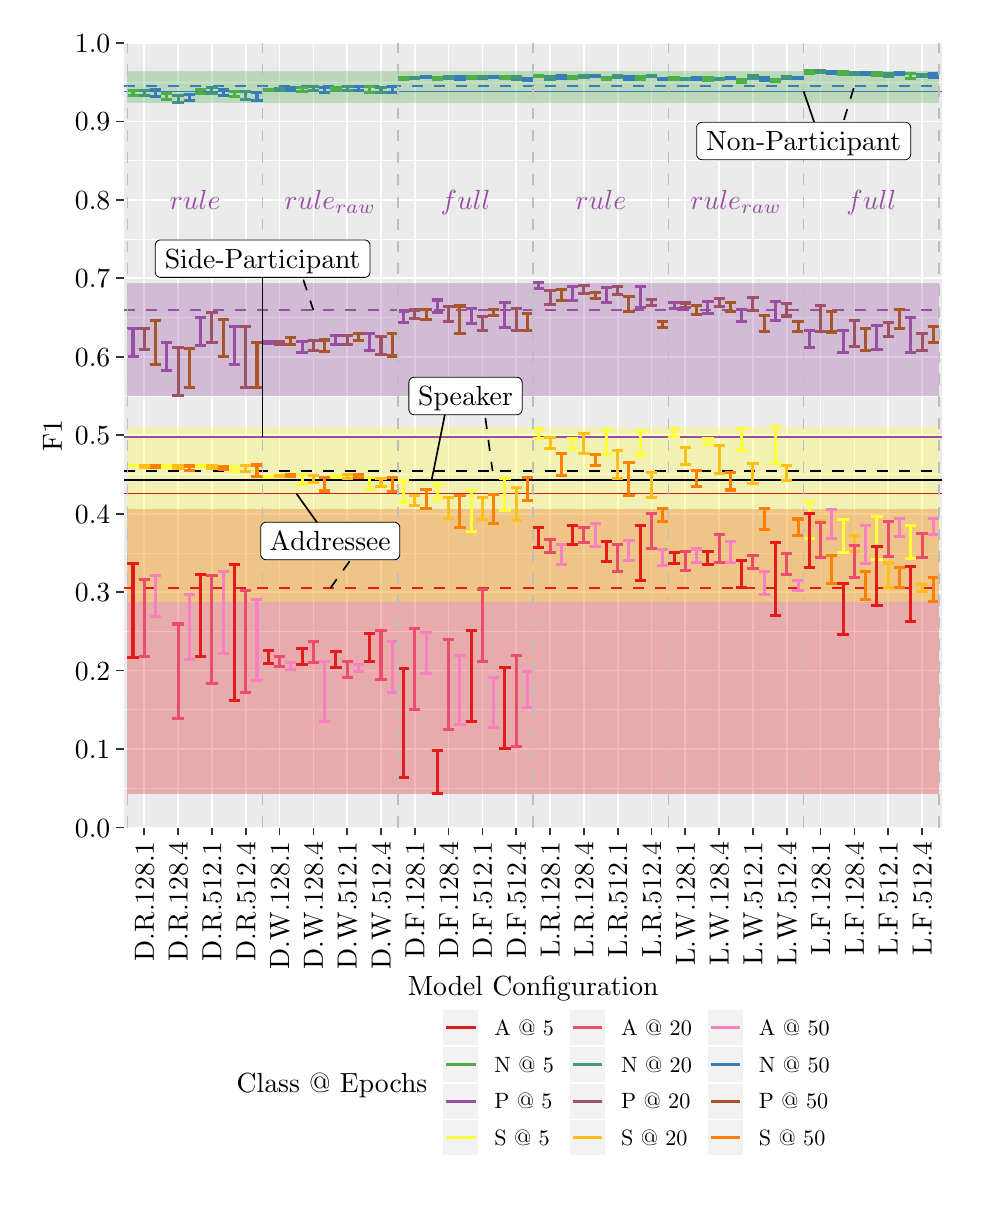
\begin{tikzpicture}[x=1pt,y=1pt]
\definecolor{fillColor}{RGB}{255,255,255}
\path[use as bounding box,fill=fillColor,fill opacity=0.00] (0,0) rectangle (336.00,415.30);
\begin{scope}
\path[clip] (  0.00,  0.00) rectangle (336.00,415.30);
\definecolor{drawColor}{RGB}{255,255,255}
\definecolor{fillColor}{RGB}{255,255,255}

\path[draw=drawColor,line width= 0.6pt,line join=round,line cap=round,fill=fillColor] (  0.00,  0.00) rectangle (336.00,415.30);
\end{scope}
\begin{scope}
\path[clip] ( 34.81,126.27) rectangle (330.50,409.80);
\definecolor{fillColor}{gray}{0.92}

\path[fill=fillColor] ( 34.81,126.27) rectangle (330.50,409.80);
\definecolor{drawColor}{RGB}{255,255,255}

\path[draw=drawColor,line width= 0.3pt,line join=round] ( 34.81,140.44) --
	(330.50,140.44);

\path[draw=drawColor,line width= 0.3pt,line join=round] ( 34.81,168.80) --
	(330.50,168.80);

\path[draw=drawColor,line width= 0.3pt,line join=round] ( 34.81,197.15) --
	(330.50,197.15);

\path[draw=drawColor,line width= 0.3pt,line join=round] ( 34.81,225.50) --
	(330.50,225.50);

\path[draw=drawColor,line width= 0.3pt,line join=round] ( 34.81,253.86) --
	(330.50,253.86);

\path[draw=drawColor,line width= 0.3pt,line join=round] ( 34.81,282.21) --
	(330.50,282.21);

\path[draw=drawColor,line width= 0.3pt,line join=round] ( 34.81,310.56) --
	(330.50,310.56);

\path[draw=drawColor,line width= 0.3pt,line join=round] ( 34.81,338.91) --
	(330.50,338.91);

\path[draw=drawColor,line width= 0.3pt,line join=round] ( 34.81,367.27) --
	(330.50,367.27);

\path[draw=drawColor,line width= 0.3pt,line join=round] ( 34.81,395.62) --
	(330.50,395.62);

\path[draw=drawColor,line width= 0.6pt,line join=round] ( 34.81,126.27) --
	(330.50,126.27);

\path[draw=drawColor,line width= 0.6pt,line join=round] ( 34.81,154.62) --
	(330.50,154.62);

\path[draw=drawColor,line width= 0.6pt,line join=round] ( 34.81,182.97) --
	(330.50,182.97);

\path[draw=drawColor,line width= 0.6pt,line join=round] ( 34.81,211.33) --
	(330.50,211.33);

\path[draw=drawColor,line width= 0.6pt,line join=round] ( 34.81,239.68) --
	(330.50,239.68);

\path[draw=drawColor,line width= 0.6pt,line join=round] ( 34.81,268.03) --
	(330.50,268.03);

\path[draw=drawColor,line width= 0.6pt,line join=round] ( 34.81,296.38) --
	(330.50,296.38);

\path[draw=drawColor,line width= 0.6pt,line join=round] ( 34.81,324.74) --
	(330.50,324.74);

\path[draw=drawColor,line width= 0.6pt,line join=round] ( 34.81,353.09) --
	(330.50,353.09);

\path[draw=drawColor,line width= 0.6pt,line join=round] ( 34.81,381.44) --
	(330.50,381.44);

\path[draw=drawColor,line width= 0.6pt,line join=round] ( 34.81,409.80) --
	(330.50,409.80);

\path[draw=drawColor,line width= 0.6pt,line join=round] ( 42.14,126.27) --
	( 42.14,409.80);

\path[draw=drawColor,line width= 0.6pt,line join=round] ( 54.36,126.27) --
	( 54.36,409.80);

\path[draw=drawColor,line width= 0.6pt,line join=round] ( 66.57,126.27) --
	( 66.57,409.80);

\path[draw=drawColor,line width= 0.6pt,line join=round] ( 78.79,126.27) --
	( 78.79,409.80);

\path[draw=drawColor,line width= 0.6pt,line join=round] ( 91.01,126.27) --
	( 91.01,409.80);

\path[draw=drawColor,line width= 0.6pt,line join=round] (103.23,126.27) --
	(103.23,409.80);

\path[draw=drawColor,line width= 0.6pt,line join=round] (115.45,126.27) --
	(115.45,409.80);

\path[draw=drawColor,line width= 0.6pt,line join=round] (127.67,126.27) --
	(127.67,409.80);

\path[draw=drawColor,line width= 0.6pt,line join=round] (139.89,126.27) --
	(139.89,409.80);

\path[draw=drawColor,line width= 0.6pt,line join=round] (152.11,126.27) --
	(152.11,409.80);

\path[draw=drawColor,line width= 0.6pt,line join=round] (164.32,126.27) --
	(164.32,409.80);

\path[draw=drawColor,line width= 0.6pt,line join=round] (176.54,126.27) --
	(176.54,409.80);

\path[draw=drawColor,line width= 0.6pt,line join=round] (188.76,126.27) --
	(188.76,409.80);

\path[draw=drawColor,line width= 0.6pt,line join=round] (200.98,126.27) --
	(200.98,409.80);

\path[draw=drawColor,line width= 0.6pt,line join=round] (213.20,126.27) --
	(213.20,409.80);

\path[draw=drawColor,line width= 0.6pt,line join=round] (225.42,126.27) --
	(225.42,409.80);

\path[draw=drawColor,line width= 0.6pt,line join=round] (237.64,126.27) --
	(237.64,409.80);

\path[draw=drawColor,line width= 0.6pt,line join=round] (249.86,126.27) --
	(249.86,409.80);

\path[draw=drawColor,line width= 0.6pt,line join=round] (262.07,126.27) --
	(262.07,409.80);

\path[draw=drawColor,line width= 0.6pt,line join=round] (274.29,126.27) --
	(274.29,409.80);

\path[draw=drawColor,line width= 0.6pt,line join=round] (286.51,126.27) --
	(286.51,409.80);

\path[draw=drawColor,line width= 0.6pt,line join=round] (298.73,126.27) --
	(298.73,409.80);

\path[draw=drawColor,line width= 0.6pt,line join=round] (310.95,126.27) --
	(310.95,409.80);

\path[draw=drawColor,line width= 0.6pt,line join=round] (323.17,126.27) --
	(323.17,409.80);
\definecolor{fillColor}{RGB}{228,26,28}

\path[fill=fillColor,fill opacity=0.30] ( 36.03,138.45) rectangle (329.28,241.21);
\definecolor{fillColor}{RGB}{255,255,51}

\path[fill=fillColor,fill opacity=0.30] ( 36.03,207.85) rectangle (329.28,271.07);
\definecolor{fillColor}{RGB}{152,78,163}

\path[fill=fillColor,fill opacity=0.30] ( 36.03,282.27) rectangle (329.28,323.05);
\definecolor{fillColor}{RGB}{77,175,74}

\path[fill=fillColor,fill opacity=0.30] ( 36.03,388.19) rectangle (329.28,399.75);
\definecolor{drawColor}{RGB}{0,0,0}

\path[draw=drawColor,line width= 0.6pt,line join=round] ( 34.81,251.92) -- (330.50,251.92);
\definecolor{drawColor}{RGB}{55,126,184}

\path[draw=drawColor,line width= 0.6pt,line join=round] ( 34.81,392.29) -- (330.50,392.29);
\definecolor{drawColor}{RGB}{228,26,28}

\path[draw=drawColor,line width= 0.6pt,line join=round] ( 34.81,246.92) -- (330.50,246.92);
\definecolor{drawColor}{RGB}{152,78,163}

\path[draw=drawColor,line width= 0.6pt,line join=round] ( 34.81,267.34) -- (330.50,267.34);
\definecolor{drawColor}{RGB}{0,0,0}

\path[draw=drawColor,line width= 0.6pt,dash pattern=on 4pt off 4pt ,line join=round] ( 34.81,255.05) -- (330.50,255.05);
\definecolor{drawColor}{RGB}{55,126,184}

\path[draw=drawColor,line width= 0.6pt,dash pattern=on 4pt off 4pt ,line join=round] ( 34.81,394.22) -- (330.50,394.22);
\definecolor{drawColor}{RGB}{228,26,28}

\path[draw=drawColor,line width= 0.6pt,dash pattern=on 4pt off 4pt ,line join=round] ( 34.81,212.71) -- (330.50,212.71);
\definecolor{drawColor}{RGB}{152,78,163}

\path[draw=drawColor,line width= 0.6pt,dash pattern=on 4pt off 4pt ,line join=round] ( 34.81,313.22) -- (330.50,313.22);
\definecolor{drawColor}{RGB}{255,127,0}

\path[draw=drawColor,line width= 1.1pt,line join=round] ( 44.17,257.22) --
	( 48.25,257.22);

\path[draw=drawColor,line width= 1.1pt,line join=round] ( 46.21,257.22) --
	( 46.21,256.40);

\path[draw=drawColor,line width= 1.1pt,line join=round] ( 44.17,256.40) --
	( 48.25,256.40);

\path[draw=drawColor,line width= 1.1pt,line join=round] ( 44.17,257.22) --
	( 48.25,257.22);

\path[draw=drawColor,line width= 1.1pt,line join=round] ( 46.21,257.22) --
	( 46.21,256.40);

\path[draw=drawColor,line width= 1.1pt,line join=round] ( 44.17,256.40) --
	( 48.25,256.40);

\path[draw=drawColor,line width= 1.1pt,line join=round] ( 44.17,257.22) --
	( 48.25,257.22);

\path[draw=drawColor,line width= 1.1pt,line join=round] ( 46.21,257.22) --
	( 46.21,256.40);

\path[draw=drawColor,line width= 1.1pt,line join=round] ( 44.17,256.40) --
	( 48.25,256.40);

\path[draw=drawColor,line width= 1.1pt,line join=round] ( 44.17,257.22) --
	( 48.25,257.22);

\path[draw=drawColor,line width= 1.1pt,line join=round] ( 46.21,257.22) --
	( 46.21,256.40);

\path[draw=drawColor,line width= 1.1pt,line join=round] ( 44.17,256.40) --
	( 48.25,256.40);

\path[draw=drawColor,line width= 1.1pt,line join=round] ( 44.17,257.22) --
	( 48.25,257.22);

\path[draw=drawColor,line width= 1.1pt,line join=round] ( 46.21,257.22) --
	( 46.21,256.40);

\path[draw=drawColor,line width= 1.1pt,line join=round] ( 44.17,256.40) --
	( 48.25,256.40);

\path[draw=drawColor,line width= 1.1pt,line join=round] ( 44.17,257.22) --
	( 48.25,257.22);

\path[draw=drawColor,line width= 1.1pt,line join=round] ( 46.21,257.22) --
	( 46.21,256.40);

\path[draw=drawColor,line width= 1.1pt,line join=round] ( 44.17,256.40) --
	( 48.25,256.40);

\path[draw=drawColor,line width= 1.1pt,line join=round] ( 44.17,257.22) --
	( 48.25,257.22);

\path[draw=drawColor,line width= 1.1pt,line join=round] ( 46.21,257.22) --
	( 46.21,256.40);

\path[draw=drawColor,line width= 1.1pt,line join=round] ( 44.17,256.40) --
	( 48.25,256.40);

\path[draw=drawColor,line width= 1.1pt,line join=round] ( 44.17,257.22) --
	( 48.25,257.22);

\path[draw=drawColor,line width= 1.1pt,line join=round] ( 46.21,257.22) --
	( 46.21,256.40);

\path[draw=drawColor,line width= 1.1pt,line join=round] ( 44.17,256.40) --
	( 48.25,256.40);
\definecolor{drawColor}{RGB}{255,191,25}

\path[draw=drawColor,line width= 1.1pt,line join=round] ( 40.10,257.05) --
	( 44.17,257.05);

\path[draw=drawColor,line width= 1.1pt,line join=round] ( 42.14,257.05) --
	( 42.14,256.34);

\path[draw=drawColor,line width= 1.1pt,line join=round] ( 40.10,256.34) --
	( 44.17,256.34);

\path[draw=drawColor,line width= 1.1pt,line join=round] ( 40.10,257.05) --
	( 44.17,257.05);

\path[draw=drawColor,line width= 1.1pt,line join=round] ( 42.14,257.05) --
	( 42.14,256.34);

\path[draw=drawColor,line width= 1.1pt,line join=round] ( 40.10,256.34) --
	( 44.17,256.34);

\path[draw=drawColor,line width= 1.1pt,line join=round] ( 40.10,257.05) --
	( 44.17,257.05);

\path[draw=drawColor,line width= 1.1pt,line join=round] ( 42.14,257.05) --
	( 42.14,256.34);

\path[draw=drawColor,line width= 1.1pt,line join=round] ( 40.10,256.34) --
	( 44.17,256.34);

\path[draw=drawColor,line width= 1.1pt,line join=round] ( 40.10,257.05) --
	( 44.17,257.05);

\path[draw=drawColor,line width= 1.1pt,line join=round] ( 42.14,257.05) --
	( 42.14,256.34);

\path[draw=drawColor,line width= 1.1pt,line join=round] ( 40.10,256.34) --
	( 44.17,256.34);

\path[draw=drawColor,line width= 1.1pt,line join=round] ( 40.10,257.05) --
	( 44.17,257.05);

\path[draw=drawColor,line width= 1.1pt,line join=round] ( 42.14,257.05) --
	( 42.14,256.34);

\path[draw=drawColor,line width= 1.1pt,line join=round] ( 40.10,256.34) --
	( 44.17,256.34);

\path[draw=drawColor,line width= 1.1pt,line join=round] ( 40.10,257.05) --
	( 44.17,257.05);

\path[draw=drawColor,line width= 1.1pt,line join=round] ( 42.14,257.05) --
	( 42.14,256.34);

\path[draw=drawColor,line width= 1.1pt,line join=round] ( 40.10,256.34) --
	( 44.17,256.34);

\path[draw=drawColor,line width= 1.1pt,line join=round] ( 40.10,257.05) --
	( 44.17,257.05);

\path[draw=drawColor,line width= 1.1pt,line join=round] ( 42.14,257.05) --
	( 42.14,256.34);

\path[draw=drawColor,line width= 1.1pt,line join=round] ( 40.10,256.34) --
	( 44.17,256.34);

\path[draw=drawColor,line width= 1.1pt,line join=round] ( 40.10,257.05) --
	( 44.17,257.05);

\path[draw=drawColor,line width= 1.1pt,line join=round] ( 42.14,257.05) --
	( 42.14,256.34);

\path[draw=drawColor,line width= 1.1pt,line join=round] ( 40.10,256.34) --
	( 44.17,256.34);
\definecolor{drawColor}{RGB}{255,255,51}

\path[draw=drawColor,line width= 1.1pt,line join=round] ( 36.03,257.26) --
	( 40.10,257.26);

\path[draw=drawColor,line width= 1.1pt,line join=round] ( 38.06,257.26) --
	( 38.06,256.93);

\path[draw=drawColor,line width= 1.1pt,line join=round] ( 36.03,256.93) --
	( 40.10,256.93);

\path[draw=drawColor,line width= 1.1pt,line join=round] ( 36.03,257.26) --
	( 40.10,257.26);

\path[draw=drawColor,line width= 1.1pt,line join=round] ( 38.06,257.26) --
	( 38.06,256.93);

\path[draw=drawColor,line width= 1.1pt,line join=round] ( 36.03,256.93) --
	( 40.10,256.93);

\path[draw=drawColor,line width= 1.1pt,line join=round] ( 36.03,257.26) --
	( 40.10,257.26);

\path[draw=drawColor,line width= 1.1pt,line join=round] ( 38.06,257.26) --
	( 38.06,256.93);

\path[draw=drawColor,line width= 1.1pt,line join=round] ( 36.03,256.93) --
	( 40.10,256.93);

\path[draw=drawColor,line width= 1.1pt,line join=round] ( 36.03,257.26) --
	( 40.10,257.26);

\path[draw=drawColor,line width= 1.1pt,line join=round] ( 38.06,257.26) --
	( 38.06,256.93);

\path[draw=drawColor,line width= 1.1pt,line join=round] ( 36.03,256.93) --
	( 40.10,256.93);

\path[draw=drawColor,line width= 1.1pt,line join=round] ( 36.03,257.26) --
	( 40.10,257.26);

\path[draw=drawColor,line width= 1.1pt,line join=round] ( 38.06,257.26) --
	( 38.06,256.93);

\path[draw=drawColor,line width= 1.1pt,line join=round] ( 36.03,256.93) --
	( 40.10,256.93);

\path[draw=drawColor,line width= 1.1pt,line join=round] ( 36.03,257.26) --
	( 40.10,257.26);

\path[draw=drawColor,line width= 1.1pt,line join=round] ( 38.06,257.26) --
	( 38.06,256.93);

\path[draw=drawColor,line width= 1.1pt,line join=round] ( 36.03,256.93) --
	( 40.10,256.93);

\path[draw=drawColor,line width= 1.1pt,line join=round] ( 36.03,257.26) --
	( 40.10,257.26);

\path[draw=drawColor,line width= 1.1pt,line join=round] ( 38.06,257.26) --
	( 38.06,256.93);

\path[draw=drawColor,line width= 1.1pt,line join=round] ( 36.03,256.93) --
	( 40.10,256.93);

\path[draw=drawColor,line width= 1.1pt,line join=round] ( 36.03,257.26) --
	( 40.10,257.26);

\path[draw=drawColor,line width= 1.1pt,line join=round] ( 38.06,257.26) --
	( 38.06,256.93);

\path[draw=drawColor,line width= 1.1pt,line join=round] ( 36.03,256.93) --
	( 40.10,256.93);
\definecolor{drawColor}{RGB}{255,127,0}

\path[draw=drawColor,line width= 1.1pt,line join=round] ( 56.39,256.90) --
	( 60.47,256.90);

\path[draw=drawColor,line width= 1.1pt,line join=round] ( 58.43,256.90) --
	( 58.43,255.41);

\path[draw=drawColor,line width= 1.1pt,line join=round] ( 56.39,255.41) --
	( 60.47,255.41);

\path[draw=drawColor,line width= 1.1pt,line join=round] ( 56.39,256.90) --
	( 60.47,256.90);

\path[draw=drawColor,line width= 1.1pt,line join=round] ( 58.43,256.90) --
	( 58.43,255.41);

\path[draw=drawColor,line width= 1.1pt,line join=round] ( 56.39,255.41) --
	( 60.47,255.41);

\path[draw=drawColor,line width= 1.1pt,line join=round] ( 56.39,256.90) --
	( 60.47,256.90);

\path[draw=drawColor,line width= 1.1pt,line join=round] ( 58.43,256.90) --
	( 58.43,255.41);

\path[draw=drawColor,line width= 1.1pt,line join=round] ( 56.39,255.41) --
	( 60.47,255.41);

\path[draw=drawColor,line width= 1.1pt,line join=round] ( 56.39,256.90) --
	( 60.47,256.90);

\path[draw=drawColor,line width= 1.1pt,line join=round] ( 58.43,256.90) --
	( 58.43,255.41);

\path[draw=drawColor,line width= 1.1pt,line join=round] ( 56.39,255.41) --
	( 60.47,255.41);

\path[draw=drawColor,line width= 1.1pt,line join=round] ( 56.39,256.90) --
	( 60.47,256.90);

\path[draw=drawColor,line width= 1.1pt,line join=round] ( 58.43,256.90) --
	( 58.43,255.41);

\path[draw=drawColor,line width= 1.1pt,line join=round] ( 56.39,255.41) --
	( 60.47,255.41);

\path[draw=drawColor,line width= 1.1pt,line join=round] ( 56.39,256.90) --
	( 60.47,256.90);

\path[draw=drawColor,line width= 1.1pt,line join=round] ( 58.43,256.90) --
	( 58.43,255.41);

\path[draw=drawColor,line width= 1.1pt,line join=round] ( 56.39,255.41) --
	( 60.47,255.41);

\path[draw=drawColor,line width= 1.1pt,line join=round] ( 56.39,256.90) --
	( 60.47,256.90);

\path[draw=drawColor,line width= 1.1pt,line join=round] ( 58.43,256.90) --
	( 58.43,255.41);

\path[draw=drawColor,line width= 1.1pt,line join=round] ( 56.39,255.41) --
	( 60.47,255.41);

\path[draw=drawColor,line width= 1.1pt,line join=round] ( 56.39,256.90) --
	( 60.47,256.90);

\path[draw=drawColor,line width= 1.1pt,line join=round] ( 58.43,256.90) --
	( 58.43,255.41);

\path[draw=drawColor,line width= 1.1pt,line join=round] ( 56.39,255.41) --
	( 60.47,255.41);
\definecolor{drawColor}{RGB}{255,191,25}

\path[draw=drawColor,line width= 1.1pt,line join=round] ( 52.32,257.15) --
	( 56.39,257.15);

\path[draw=drawColor,line width= 1.1pt,line join=round] ( 54.36,257.15) --
	( 54.36,255.99);

\path[draw=drawColor,line width= 1.1pt,line join=round] ( 52.32,255.99) --
	( 56.39,255.99);

\path[draw=drawColor,line width= 1.1pt,line join=round] ( 52.32,257.15) --
	( 56.39,257.15);

\path[draw=drawColor,line width= 1.1pt,line join=round] ( 54.36,257.15) --
	( 54.36,255.99);

\path[draw=drawColor,line width= 1.1pt,line join=round] ( 52.32,255.99) --
	( 56.39,255.99);

\path[draw=drawColor,line width= 1.1pt,line join=round] ( 52.32,257.15) --
	( 56.39,257.15);

\path[draw=drawColor,line width= 1.1pt,line join=round] ( 54.36,257.15) --
	( 54.36,255.99);

\path[draw=drawColor,line width= 1.1pt,line join=round] ( 52.32,255.99) --
	( 56.39,255.99);

\path[draw=drawColor,line width= 1.1pt,line join=round] ( 52.32,257.15) --
	( 56.39,257.15);

\path[draw=drawColor,line width= 1.1pt,line join=round] ( 54.36,257.15) --
	( 54.36,255.99);

\path[draw=drawColor,line width= 1.1pt,line join=round] ( 52.32,255.99) --
	( 56.39,255.99);

\path[draw=drawColor,line width= 1.1pt,line join=round] ( 52.32,257.15) --
	( 56.39,257.15);

\path[draw=drawColor,line width= 1.1pt,line join=round] ( 54.36,257.15) --
	( 54.36,255.99);

\path[draw=drawColor,line width= 1.1pt,line join=round] ( 52.32,255.99) --
	( 56.39,255.99);

\path[draw=drawColor,line width= 1.1pt,line join=round] ( 52.32,257.15) --
	( 56.39,257.15);

\path[draw=drawColor,line width= 1.1pt,line join=round] ( 54.36,257.15) --
	( 54.36,255.99);

\path[draw=drawColor,line width= 1.1pt,line join=round] ( 52.32,255.99) --
	( 56.39,255.99);

\path[draw=drawColor,line width= 1.1pt,line join=round] ( 52.32,257.15) --
	( 56.39,257.15);

\path[draw=drawColor,line width= 1.1pt,line join=round] ( 54.36,257.15) --
	( 54.36,255.99);

\path[draw=drawColor,line width= 1.1pt,line join=round] ( 52.32,255.99) --
	( 56.39,255.99);

\path[draw=drawColor,line width= 1.1pt,line join=round] ( 52.32,257.15) --
	( 56.39,257.15);

\path[draw=drawColor,line width= 1.1pt,line join=round] ( 54.36,257.15) --
	( 54.36,255.99);

\path[draw=drawColor,line width= 1.1pt,line join=round] ( 52.32,255.99) --
	( 56.39,255.99);
\definecolor{drawColor}{RGB}{255,255,51}

\path[draw=drawColor,line width= 1.1pt,line join=round] ( 48.25,257.21) --
	( 52.32,257.21);

\path[draw=drawColor,line width= 1.1pt,line join=round] ( 50.28,257.21) --
	( 50.28,256.45);

\path[draw=drawColor,line width= 1.1pt,line join=round] ( 48.25,256.45) --
	( 52.32,256.45);

\path[draw=drawColor,line width= 1.1pt,line join=round] ( 48.25,257.21) --
	( 52.32,257.21);

\path[draw=drawColor,line width= 1.1pt,line join=round] ( 50.28,257.21) --
	( 50.28,256.45);

\path[draw=drawColor,line width= 1.1pt,line join=round] ( 48.25,256.45) --
	( 52.32,256.45);

\path[draw=drawColor,line width= 1.1pt,line join=round] ( 48.25,257.21) --
	( 52.32,257.21);

\path[draw=drawColor,line width= 1.1pt,line join=round] ( 50.28,257.21) --
	( 50.28,256.45);

\path[draw=drawColor,line width= 1.1pt,line join=round] ( 48.25,256.45) --
	( 52.32,256.45);

\path[draw=drawColor,line width= 1.1pt,line join=round] ( 48.25,257.21) --
	( 52.32,257.21);

\path[draw=drawColor,line width= 1.1pt,line join=round] ( 50.28,257.21) --
	( 50.28,256.45);

\path[draw=drawColor,line width= 1.1pt,line join=round] ( 48.25,256.45) --
	( 52.32,256.45);

\path[draw=drawColor,line width= 1.1pt,line join=round] ( 48.25,257.21) --
	( 52.32,257.21);

\path[draw=drawColor,line width= 1.1pt,line join=round] ( 50.28,257.21) --
	( 50.28,256.45);

\path[draw=drawColor,line width= 1.1pt,line join=round] ( 48.25,256.45) --
	( 52.32,256.45);

\path[draw=drawColor,line width= 1.1pt,line join=round] ( 48.25,257.21) --
	( 52.32,257.21);

\path[draw=drawColor,line width= 1.1pt,line join=round] ( 50.28,257.21) --
	( 50.28,256.45);

\path[draw=drawColor,line width= 1.1pt,line join=round] ( 48.25,256.45) --
	( 52.32,256.45);

\path[draw=drawColor,line width= 1.1pt,line join=round] ( 48.25,257.21) --
	( 52.32,257.21);

\path[draw=drawColor,line width= 1.1pt,line join=round] ( 50.28,257.21) --
	( 50.28,256.45);

\path[draw=drawColor,line width= 1.1pt,line join=round] ( 48.25,256.45) --
	( 52.32,256.45);

\path[draw=drawColor,line width= 1.1pt,line join=round] ( 48.25,257.21) --
	( 52.32,257.21);

\path[draw=drawColor,line width= 1.1pt,line join=round] ( 50.28,257.21) --
	( 50.28,256.45);

\path[draw=drawColor,line width= 1.1pt,line join=round] ( 48.25,256.45) --
	( 52.32,256.45);
\definecolor{drawColor}{RGB}{255,127,0}

\path[draw=drawColor,line width= 1.1pt,line join=round] ( 68.61,256.81) --
	( 72.68,256.81);

\path[draw=drawColor,line width= 1.1pt,line join=round] ( 70.65,256.81) --
	( 70.65,255.75);

\path[draw=drawColor,line width= 1.1pt,line join=round] ( 68.61,255.75) --
	( 72.68,255.75);

\path[draw=drawColor,line width= 1.1pt,line join=round] ( 68.61,256.81) --
	( 72.68,256.81);

\path[draw=drawColor,line width= 1.1pt,line join=round] ( 70.65,256.81) --
	( 70.65,255.75);

\path[draw=drawColor,line width= 1.1pt,line join=round] ( 68.61,255.75) --
	( 72.68,255.75);

\path[draw=drawColor,line width= 1.1pt,line join=round] ( 68.61,256.81) --
	( 72.68,256.81);

\path[draw=drawColor,line width= 1.1pt,line join=round] ( 70.65,256.81) --
	( 70.65,255.75);

\path[draw=drawColor,line width= 1.1pt,line join=round] ( 68.61,255.75) --
	( 72.68,255.75);

\path[draw=drawColor,line width= 1.1pt,line join=round] ( 68.61,256.81) --
	( 72.68,256.81);

\path[draw=drawColor,line width= 1.1pt,line join=round] ( 70.65,256.81) --
	( 70.65,255.75);

\path[draw=drawColor,line width= 1.1pt,line join=round] ( 68.61,255.75) --
	( 72.68,255.75);

\path[draw=drawColor,line width= 1.1pt,line join=round] ( 68.61,256.81) --
	( 72.68,256.81);

\path[draw=drawColor,line width= 1.1pt,line join=round] ( 70.65,256.81) --
	( 70.65,255.75);

\path[draw=drawColor,line width= 1.1pt,line join=round] ( 68.61,255.75) --
	( 72.68,255.75);

\path[draw=drawColor,line width= 1.1pt,line join=round] ( 68.61,256.81) --
	( 72.68,256.81);

\path[draw=drawColor,line width= 1.1pt,line join=round] ( 70.65,256.81) --
	( 70.65,255.75);

\path[draw=drawColor,line width= 1.1pt,line join=round] ( 68.61,255.75) --
	( 72.68,255.75);

\path[draw=drawColor,line width= 1.1pt,line join=round] ( 68.61,256.81) --
	( 72.68,256.81);

\path[draw=drawColor,line width= 1.1pt,line join=round] ( 70.65,256.81) --
	( 70.65,255.75);

\path[draw=drawColor,line width= 1.1pt,line join=round] ( 68.61,255.75) --
	( 72.68,255.75);

\path[draw=drawColor,line width= 1.1pt,line join=round] ( 68.61,256.81) --
	( 72.68,256.81);

\path[draw=drawColor,line width= 1.1pt,line join=round] ( 70.65,256.81) --
	( 70.65,255.75);

\path[draw=drawColor,line width= 1.1pt,line join=round] ( 68.61,255.75) --
	( 72.68,255.75);
\definecolor{drawColor}{RGB}{255,191,25}

\path[draw=drawColor,line width= 1.1pt,line join=round] ( 64.54,256.93) --
	( 68.61,256.93);

\path[draw=drawColor,line width= 1.1pt,line join=round] ( 66.57,256.93) --
	( 66.57,255.87);

\path[draw=drawColor,line width= 1.1pt,line join=round] ( 64.54,255.87) --
	( 68.61,255.87);

\path[draw=drawColor,line width= 1.1pt,line join=round] ( 64.54,256.93) --
	( 68.61,256.93);

\path[draw=drawColor,line width= 1.1pt,line join=round] ( 66.57,256.93) --
	( 66.57,255.87);

\path[draw=drawColor,line width= 1.1pt,line join=round] ( 64.54,255.87) --
	( 68.61,255.87);

\path[draw=drawColor,line width= 1.1pt,line join=round] ( 64.54,256.93) --
	( 68.61,256.93);

\path[draw=drawColor,line width= 1.1pt,line join=round] ( 66.57,256.93) --
	( 66.57,255.87);

\path[draw=drawColor,line width= 1.1pt,line join=round] ( 64.54,255.87) --
	( 68.61,255.87);

\path[draw=drawColor,line width= 1.1pt,line join=round] ( 64.54,256.93) --
	( 68.61,256.93);

\path[draw=drawColor,line width= 1.1pt,line join=round] ( 66.57,256.93) --
	( 66.57,255.87);

\path[draw=drawColor,line width= 1.1pt,line join=round] ( 64.54,255.87) --
	( 68.61,255.87);

\path[draw=drawColor,line width= 1.1pt,line join=round] ( 64.54,256.93) --
	( 68.61,256.93);

\path[draw=drawColor,line width= 1.1pt,line join=round] ( 66.57,256.93) --
	( 66.57,255.87);

\path[draw=drawColor,line width= 1.1pt,line join=round] ( 64.54,255.87) --
	( 68.61,255.87);

\path[draw=drawColor,line width= 1.1pt,line join=round] ( 64.54,256.93) --
	( 68.61,256.93);

\path[draw=drawColor,line width= 1.1pt,line join=round] ( 66.57,256.93) --
	( 66.57,255.87);

\path[draw=drawColor,line width= 1.1pt,line join=round] ( 64.54,255.87) --
	( 68.61,255.87);

\path[draw=drawColor,line width= 1.1pt,line join=round] ( 64.54,256.93) --
	( 68.61,256.93);

\path[draw=drawColor,line width= 1.1pt,line join=round] ( 66.57,256.93) --
	( 66.57,255.87);

\path[draw=drawColor,line width= 1.1pt,line join=round] ( 64.54,255.87) --
	( 68.61,255.87);

\path[draw=drawColor,line width= 1.1pt,line join=round] ( 64.54,256.93) --
	( 68.61,256.93);

\path[draw=drawColor,line width= 1.1pt,line join=round] ( 66.57,256.93) --
	( 66.57,255.87);

\path[draw=drawColor,line width= 1.1pt,line join=round] ( 64.54,255.87) --
	( 68.61,255.87);
\definecolor{drawColor}{RGB}{255,255,51}

\path[draw=drawColor,line width= 1.1pt,line join=round] ( 60.47,257.04) --
	( 64.54,257.04);

\path[draw=drawColor,line width= 1.1pt,line join=round] ( 62.50,257.04) --
	( 62.50,256.63);

\path[draw=drawColor,line width= 1.1pt,line join=round] ( 60.47,256.63) --
	( 64.54,256.63);

\path[draw=drawColor,line width= 1.1pt,line join=round] ( 60.47,257.04) --
	( 64.54,257.04);

\path[draw=drawColor,line width= 1.1pt,line join=round] ( 62.50,257.04) --
	( 62.50,256.63);

\path[draw=drawColor,line width= 1.1pt,line join=round] ( 60.47,256.63) --
	( 64.54,256.63);

\path[draw=drawColor,line width= 1.1pt,line join=round] ( 60.47,257.04) --
	( 64.54,257.04);

\path[draw=drawColor,line width= 1.1pt,line join=round] ( 62.50,257.04) --
	( 62.50,256.63);

\path[draw=drawColor,line width= 1.1pt,line join=round] ( 60.47,256.63) --
	( 64.54,256.63);

\path[draw=drawColor,line width= 1.1pt,line join=round] ( 60.47,257.04) --
	( 64.54,257.04);

\path[draw=drawColor,line width= 1.1pt,line join=round] ( 62.50,257.04) --
	( 62.50,256.63);

\path[draw=drawColor,line width= 1.1pt,line join=round] ( 60.47,256.63) --
	( 64.54,256.63);

\path[draw=drawColor,line width= 1.1pt,line join=round] ( 60.47,257.04) --
	( 64.54,257.04);

\path[draw=drawColor,line width= 1.1pt,line join=round] ( 62.50,257.04) --
	( 62.50,256.63);

\path[draw=drawColor,line width= 1.1pt,line join=round] ( 60.47,256.63) --
	( 64.54,256.63);

\path[draw=drawColor,line width= 1.1pt,line join=round] ( 60.47,257.04) --
	( 64.54,257.04);

\path[draw=drawColor,line width= 1.1pt,line join=round] ( 62.50,257.04) --
	( 62.50,256.63);

\path[draw=drawColor,line width= 1.1pt,line join=round] ( 60.47,256.63) --
	( 64.54,256.63);

\path[draw=drawColor,line width= 1.1pt,line join=round] ( 60.47,257.04) --
	( 64.54,257.04);

\path[draw=drawColor,line width= 1.1pt,line join=round] ( 62.50,257.04) --
	( 62.50,256.63);

\path[draw=drawColor,line width= 1.1pt,line join=round] ( 60.47,256.63) --
	( 64.54,256.63);

\path[draw=drawColor,line width= 1.1pt,line join=round] ( 60.47,257.04) --
	( 64.54,257.04);

\path[draw=drawColor,line width= 1.1pt,line join=round] ( 62.50,257.04) --
	( 62.50,256.63);

\path[draw=drawColor,line width= 1.1pt,line join=round] ( 60.47,256.63) --
	( 64.54,256.63);
\definecolor{drawColor}{RGB}{255,127,0}

\path[draw=drawColor,line width= 1.1pt,line join=round] ( 80.83,257.27) --
	( 84.90,257.27);

\path[draw=drawColor,line width= 1.1pt,line join=round] ( 82.87,257.27) --
	( 82.87,253.06);

\path[draw=drawColor,line width= 1.1pt,line join=round] ( 80.83,253.06) --
	( 84.90,253.06);

\path[draw=drawColor,line width= 1.1pt,line join=round] ( 80.83,257.27) --
	( 84.90,257.27);

\path[draw=drawColor,line width= 1.1pt,line join=round] ( 82.87,257.27) --
	( 82.87,253.06);

\path[draw=drawColor,line width= 1.1pt,line join=round] ( 80.83,253.06) --
	( 84.90,253.06);

\path[draw=drawColor,line width= 1.1pt,line join=round] ( 80.83,257.27) --
	( 84.90,257.27);

\path[draw=drawColor,line width= 1.1pt,line join=round] ( 82.87,257.27) --
	( 82.87,253.06);

\path[draw=drawColor,line width= 1.1pt,line join=round] ( 80.83,253.06) --
	( 84.90,253.06);

\path[draw=drawColor,line width= 1.1pt,line join=round] ( 80.83,257.27) --
	( 84.90,257.27);

\path[draw=drawColor,line width= 1.1pt,line join=round] ( 82.87,257.27) --
	( 82.87,253.06);

\path[draw=drawColor,line width= 1.1pt,line join=round] ( 80.83,253.06) --
	( 84.90,253.06);

\path[draw=drawColor,line width= 1.1pt,line join=round] ( 80.83,257.27) --
	( 84.90,257.27);

\path[draw=drawColor,line width= 1.1pt,line join=round] ( 82.87,257.27) --
	( 82.87,253.06);

\path[draw=drawColor,line width= 1.1pt,line join=round] ( 80.83,253.06) --
	( 84.90,253.06);

\path[draw=drawColor,line width= 1.1pt,line join=round] ( 80.83,257.27) --
	( 84.90,257.27);

\path[draw=drawColor,line width= 1.1pt,line join=round] ( 82.87,257.27) --
	( 82.87,253.06);

\path[draw=drawColor,line width= 1.1pt,line join=round] ( 80.83,253.06) --
	( 84.90,253.06);

\path[draw=drawColor,line width= 1.1pt,line join=round] ( 80.83,257.27) --
	( 84.90,257.27);

\path[draw=drawColor,line width= 1.1pt,line join=round] ( 82.87,257.27) --
	( 82.87,253.06);

\path[draw=drawColor,line width= 1.1pt,line join=round] ( 80.83,253.06) --
	( 84.90,253.06);

\path[draw=drawColor,line width= 1.1pt,line join=round] ( 80.83,257.27) --
	( 84.90,257.27);

\path[draw=drawColor,line width= 1.1pt,line join=round] ( 82.87,257.27) --
	( 82.87,253.06);

\path[draw=drawColor,line width= 1.1pt,line join=round] ( 80.83,253.06) --
	( 84.90,253.06);
\definecolor{drawColor}{RGB}{255,191,25}

\path[draw=drawColor,line width= 1.1pt,line join=round] ( 76.76,256.99) --
	( 80.83,256.99);

\path[draw=drawColor,line width= 1.1pt,line join=round] ( 78.79,256.99) --
	( 78.79,255.03);

\path[draw=drawColor,line width= 1.1pt,line join=round] ( 76.76,255.03) --
	( 80.83,255.03);

\path[draw=drawColor,line width= 1.1pt,line join=round] ( 76.76,256.99) --
	( 80.83,256.99);

\path[draw=drawColor,line width= 1.1pt,line join=round] ( 78.79,256.99) --
	( 78.79,255.03);

\path[draw=drawColor,line width= 1.1pt,line join=round] ( 76.76,255.03) --
	( 80.83,255.03);

\path[draw=drawColor,line width= 1.1pt,line join=round] ( 76.76,256.99) --
	( 80.83,256.99);

\path[draw=drawColor,line width= 1.1pt,line join=round] ( 78.79,256.99) --
	( 78.79,255.03);

\path[draw=drawColor,line width= 1.1pt,line join=round] ( 76.76,255.03) --
	( 80.83,255.03);

\path[draw=drawColor,line width= 1.1pt,line join=round] ( 76.76,256.99) --
	( 80.83,256.99);

\path[draw=drawColor,line width= 1.1pt,line join=round] ( 78.79,256.99) --
	( 78.79,255.03);

\path[draw=drawColor,line width= 1.1pt,line join=round] ( 76.76,255.03) --
	( 80.83,255.03);

\path[draw=drawColor,line width= 1.1pt,line join=round] ( 76.76,256.99) --
	( 80.83,256.99);

\path[draw=drawColor,line width= 1.1pt,line join=round] ( 78.79,256.99) --
	( 78.79,255.03);

\path[draw=drawColor,line width= 1.1pt,line join=round] ( 76.76,255.03) --
	( 80.83,255.03);

\path[draw=drawColor,line width= 1.1pt,line join=round] ( 76.76,256.99) --
	( 80.83,256.99);

\path[draw=drawColor,line width= 1.1pt,line join=round] ( 78.79,256.99) --
	( 78.79,255.03);

\path[draw=drawColor,line width= 1.1pt,line join=round] ( 76.76,255.03) --
	( 80.83,255.03);

\path[draw=drawColor,line width= 1.1pt,line join=round] ( 76.76,256.99) --
	( 80.83,256.99);

\path[draw=drawColor,line width= 1.1pt,line join=round] ( 78.79,256.99) --
	( 78.79,255.03);

\path[draw=drawColor,line width= 1.1pt,line join=round] ( 76.76,255.03) --
	( 80.83,255.03);

\path[draw=drawColor,line width= 1.1pt,line join=round] ( 76.76,256.99) --
	( 80.83,256.99);

\path[draw=drawColor,line width= 1.1pt,line join=round] ( 78.79,256.99) --
	( 78.79,255.03);

\path[draw=drawColor,line width= 1.1pt,line join=round] ( 76.76,255.03) --
	( 80.83,255.03);
\definecolor{drawColor}{RGB}{255,255,51}

\path[draw=drawColor,line width= 1.1pt,line join=round] ( 72.68,256.68) --
	( 76.76,256.68);

\path[draw=drawColor,line width= 1.1pt,line join=round] ( 74.72,256.68) --
	( 74.72,254.96);

\path[draw=drawColor,line width= 1.1pt,line join=round] ( 72.68,254.96) --
	( 76.76,254.96);

\path[draw=drawColor,line width= 1.1pt,line join=round] ( 72.68,256.68) --
	( 76.76,256.68);

\path[draw=drawColor,line width= 1.1pt,line join=round] ( 74.72,256.68) --
	( 74.72,254.96);

\path[draw=drawColor,line width= 1.1pt,line join=round] ( 72.68,254.96) --
	( 76.76,254.96);

\path[draw=drawColor,line width= 1.1pt,line join=round] ( 72.68,256.68) --
	( 76.76,256.68);

\path[draw=drawColor,line width= 1.1pt,line join=round] ( 74.72,256.68) --
	( 74.72,254.96);

\path[draw=drawColor,line width= 1.1pt,line join=round] ( 72.68,254.96) --
	( 76.76,254.96);

\path[draw=drawColor,line width= 1.1pt,line join=round] ( 72.68,256.68) --
	( 76.76,256.68);

\path[draw=drawColor,line width= 1.1pt,line join=round] ( 74.72,256.68) --
	( 74.72,254.96);

\path[draw=drawColor,line width= 1.1pt,line join=round] ( 72.68,254.96) --
	( 76.76,254.96);

\path[draw=drawColor,line width= 1.1pt,line join=round] ( 72.68,256.68) --
	( 76.76,256.68);

\path[draw=drawColor,line width= 1.1pt,line join=round] ( 74.72,256.68) --
	( 74.72,254.96);

\path[draw=drawColor,line width= 1.1pt,line join=round] ( 72.68,254.96) --
	( 76.76,254.96);

\path[draw=drawColor,line width= 1.1pt,line join=round] ( 72.68,256.68) --
	( 76.76,256.68);

\path[draw=drawColor,line width= 1.1pt,line join=round] ( 74.72,256.68) --
	( 74.72,254.96);

\path[draw=drawColor,line width= 1.1pt,line join=round] ( 72.68,254.96) --
	( 76.76,254.96);

\path[draw=drawColor,line width= 1.1pt,line join=round] ( 72.68,256.68) --
	( 76.76,256.68);

\path[draw=drawColor,line width= 1.1pt,line join=round] ( 74.72,256.68) --
	( 74.72,254.96);

\path[draw=drawColor,line width= 1.1pt,line join=round] ( 72.68,254.96) --
	( 76.76,254.96);

\path[draw=drawColor,line width= 1.1pt,line join=round] ( 72.68,256.68) --
	( 76.76,256.68);

\path[draw=drawColor,line width= 1.1pt,line join=round] ( 74.72,256.68) --
	( 74.72,254.96);

\path[draw=drawColor,line width= 1.1pt,line join=round] ( 72.68,254.96) --
	( 76.76,254.96);
\definecolor{drawColor}{RGB}{255,127,0}

\path[draw=drawColor,line width= 1.1pt,line join=round] ( 93.05,253.72) --
	( 97.12,253.72);

\path[draw=drawColor,line width= 1.1pt,line join=round] ( 95.09,253.72) --
	( 95.09,253.07);

\path[draw=drawColor,line width= 1.1pt,line join=round] ( 93.05,253.07) --
	( 97.12,253.07);

\path[draw=drawColor,line width= 1.1pt,line join=round] ( 93.05,253.72) --
	( 97.12,253.72);

\path[draw=drawColor,line width= 1.1pt,line join=round] ( 95.09,253.72) --
	( 95.09,253.07);

\path[draw=drawColor,line width= 1.1pt,line join=round] ( 93.05,253.07) --
	( 97.12,253.07);

\path[draw=drawColor,line width= 1.1pt,line join=round] ( 93.05,253.72) --
	( 97.12,253.72);

\path[draw=drawColor,line width= 1.1pt,line join=round] ( 95.09,253.72) --
	( 95.09,253.07);

\path[draw=drawColor,line width= 1.1pt,line join=round] ( 93.05,253.07) --
	( 97.12,253.07);

\path[draw=drawColor,line width= 1.1pt,line join=round] ( 93.05,253.72) --
	( 97.12,253.72);

\path[draw=drawColor,line width= 1.1pt,line join=round] ( 95.09,253.72) --
	( 95.09,253.07);

\path[draw=drawColor,line width= 1.1pt,line join=round] ( 93.05,253.07) --
	( 97.12,253.07);

\path[draw=drawColor,line width= 1.1pt,line join=round] ( 93.05,253.72) --
	( 97.12,253.72);

\path[draw=drawColor,line width= 1.1pt,line join=round] ( 95.09,253.72) --
	( 95.09,253.07);

\path[draw=drawColor,line width= 1.1pt,line join=round] ( 93.05,253.07) --
	( 97.12,253.07);

\path[draw=drawColor,line width= 1.1pt,line join=round] ( 93.05,253.72) --
	( 97.12,253.72);

\path[draw=drawColor,line width= 1.1pt,line join=round] ( 95.09,253.72) --
	( 95.09,253.07);

\path[draw=drawColor,line width= 1.1pt,line join=round] ( 93.05,253.07) --
	( 97.12,253.07);

\path[draw=drawColor,line width= 1.1pt,line join=round] ( 93.05,253.72) --
	( 97.12,253.72);

\path[draw=drawColor,line width= 1.1pt,line join=round] ( 95.09,253.72) --
	( 95.09,253.07);

\path[draw=drawColor,line width= 1.1pt,line join=round] ( 93.05,253.07) --
	( 97.12,253.07);

\path[draw=drawColor,line width= 1.1pt,line join=round] ( 93.05,253.72) --
	( 97.12,253.72);

\path[draw=drawColor,line width= 1.1pt,line join=round] ( 95.09,253.72) --
	( 95.09,253.07);

\path[draw=drawColor,line width= 1.1pt,line join=round] ( 93.05,253.07) --
	( 97.12,253.07);
\definecolor{drawColor}{RGB}{255,191,25}

\path[draw=drawColor,line width= 1.1pt,line join=round] ( 88.98,253.59) --
	( 93.05,253.59);

\path[draw=drawColor,line width= 1.1pt,line join=round] ( 91.01,253.59) --
	( 91.01,252.99);

\path[draw=drawColor,line width= 1.1pt,line join=round] ( 88.98,252.99) --
	( 93.05,252.99);

\path[draw=drawColor,line width= 1.1pt,line join=round] ( 88.98,253.59) --
	( 93.05,253.59);

\path[draw=drawColor,line width= 1.1pt,line join=round] ( 91.01,253.59) --
	( 91.01,252.99);

\path[draw=drawColor,line width= 1.1pt,line join=round] ( 88.98,252.99) --
	( 93.05,252.99);

\path[draw=drawColor,line width= 1.1pt,line join=round] ( 88.98,253.59) --
	( 93.05,253.59);

\path[draw=drawColor,line width= 1.1pt,line join=round] ( 91.01,253.59) --
	( 91.01,252.99);

\path[draw=drawColor,line width= 1.1pt,line join=round] ( 88.98,252.99) --
	( 93.05,252.99);

\path[draw=drawColor,line width= 1.1pt,line join=round] ( 88.98,253.59) --
	( 93.05,253.59);

\path[draw=drawColor,line width= 1.1pt,line join=round] ( 91.01,253.59) --
	( 91.01,252.99);

\path[draw=drawColor,line width= 1.1pt,line join=round] ( 88.98,252.99) --
	( 93.05,252.99);

\path[draw=drawColor,line width= 1.1pt,line join=round] ( 88.98,253.59) --
	( 93.05,253.59);

\path[draw=drawColor,line width= 1.1pt,line join=round] ( 91.01,253.59) --
	( 91.01,252.99);

\path[draw=drawColor,line width= 1.1pt,line join=round] ( 88.98,252.99) --
	( 93.05,252.99);

\path[draw=drawColor,line width= 1.1pt,line join=round] ( 88.98,253.59) --
	( 93.05,253.59);

\path[draw=drawColor,line width= 1.1pt,line join=round] ( 91.01,253.59) --
	( 91.01,252.99);

\path[draw=drawColor,line width= 1.1pt,line join=round] ( 88.98,252.99) --
	( 93.05,252.99);

\path[draw=drawColor,line width= 1.1pt,line join=round] ( 88.98,253.59) --
	( 93.05,253.59);

\path[draw=drawColor,line width= 1.1pt,line join=round] ( 91.01,253.59) --
	( 91.01,252.99);

\path[draw=drawColor,line width= 1.1pt,line join=round] ( 88.98,252.99) --
	( 93.05,252.99);

\path[draw=drawColor,line width= 1.1pt,line join=round] ( 88.98,253.59) --
	( 93.05,253.59);

\path[draw=drawColor,line width= 1.1pt,line join=round] ( 91.01,253.59) --
	( 91.01,252.99);

\path[draw=drawColor,line width= 1.1pt,line join=round] ( 88.98,252.99) --
	( 93.05,252.99);
\definecolor{drawColor}{RGB}{255,255,51}

\path[draw=drawColor,line width= 1.1pt,line join=round] ( 84.90,253.12) --
	( 88.98,253.12);

\path[draw=drawColor,line width= 1.1pt,line join=round] ( 86.94,253.12) --
	( 86.94,252.80);

\path[draw=drawColor,line width= 1.1pt,line join=round] ( 84.90,252.80) --
	( 88.98,252.80);

\path[draw=drawColor,line width= 1.1pt,line join=round] ( 84.90,253.12) --
	( 88.98,253.12);

\path[draw=drawColor,line width= 1.1pt,line join=round] ( 86.94,253.12) --
	( 86.94,252.80);

\path[draw=drawColor,line width= 1.1pt,line join=round] ( 84.90,252.80) --
	( 88.98,252.80);

\path[draw=drawColor,line width= 1.1pt,line join=round] ( 84.90,253.12) --
	( 88.98,253.12);

\path[draw=drawColor,line width= 1.1pt,line join=round] ( 86.94,253.12) --
	( 86.94,252.80);

\path[draw=drawColor,line width= 1.1pt,line join=round] ( 84.90,252.80) --
	( 88.98,252.80);

\path[draw=drawColor,line width= 1.1pt,line join=round] ( 84.90,253.12) --
	( 88.98,253.12);

\path[draw=drawColor,line width= 1.1pt,line join=round] ( 86.94,253.12) --
	( 86.94,252.80);

\path[draw=drawColor,line width= 1.1pt,line join=round] ( 84.90,252.80) --
	( 88.98,252.80);

\path[draw=drawColor,line width= 1.1pt,line join=round] ( 84.90,253.12) --
	( 88.98,253.12);

\path[draw=drawColor,line width= 1.1pt,line join=round] ( 86.94,253.12) --
	( 86.94,252.80);

\path[draw=drawColor,line width= 1.1pt,line join=round] ( 84.90,252.80) --
	( 88.98,252.80);

\path[draw=drawColor,line width= 1.1pt,line join=round] ( 84.90,253.12) --
	( 88.98,253.12);

\path[draw=drawColor,line width= 1.1pt,line join=round] ( 86.94,253.12) --
	( 86.94,252.80);

\path[draw=drawColor,line width= 1.1pt,line join=round] ( 84.90,252.80) --
	( 88.98,252.80);

\path[draw=drawColor,line width= 1.1pt,line join=round] ( 84.90,253.12) --
	( 88.98,253.12);

\path[draw=drawColor,line width= 1.1pt,line join=round] ( 86.94,253.12) --
	( 86.94,252.80);

\path[draw=drawColor,line width= 1.1pt,line join=round] ( 84.90,252.80) --
	( 88.98,252.80);

\path[draw=drawColor,line width= 1.1pt,line join=round] ( 84.90,253.12) --
	( 88.98,253.12);

\path[draw=drawColor,line width= 1.1pt,line join=round] ( 86.94,253.12) --
	( 86.94,252.80);

\path[draw=drawColor,line width= 1.1pt,line join=round] ( 84.90,252.80) --
	( 88.98,252.80);
\definecolor{drawColor}{RGB}{255,127,0}

\path[draw=drawColor,line width= 1.1pt,line join=round] (105.27,252.86) --
	(109.34,252.86);

\path[draw=drawColor,line width= 1.1pt,line join=round] (107.30,252.86) --
	(107.30,247.88);

\path[draw=drawColor,line width= 1.1pt,line join=round] (105.27,247.88) --
	(109.34,247.88);

\path[draw=drawColor,line width= 1.1pt,line join=round] (105.27,252.86) --
	(109.34,252.86);

\path[draw=drawColor,line width= 1.1pt,line join=round] (107.30,252.86) --
	(107.30,247.88);

\path[draw=drawColor,line width= 1.1pt,line join=round] (105.27,247.88) --
	(109.34,247.88);

\path[draw=drawColor,line width= 1.1pt,line join=round] (105.27,252.86) --
	(109.34,252.86);

\path[draw=drawColor,line width= 1.1pt,line join=round] (107.30,252.86) --
	(107.30,247.88);

\path[draw=drawColor,line width= 1.1pt,line join=round] (105.27,247.88) --
	(109.34,247.88);

\path[draw=drawColor,line width= 1.1pt,line join=round] (105.27,252.86) --
	(109.34,252.86);

\path[draw=drawColor,line width= 1.1pt,line join=round] (107.30,252.86) --
	(107.30,247.88);

\path[draw=drawColor,line width= 1.1pt,line join=round] (105.27,247.88) --
	(109.34,247.88);

\path[draw=drawColor,line width= 1.1pt,line join=round] (105.27,252.86) --
	(109.34,252.86);

\path[draw=drawColor,line width= 1.1pt,line join=round] (107.30,252.86) --
	(107.30,247.88);

\path[draw=drawColor,line width= 1.1pt,line join=round] (105.27,247.88) --
	(109.34,247.88);

\path[draw=drawColor,line width= 1.1pt,line join=round] (105.27,252.86) --
	(109.34,252.86);

\path[draw=drawColor,line width= 1.1pt,line join=round] (107.30,252.86) --
	(107.30,247.88);

\path[draw=drawColor,line width= 1.1pt,line join=round] (105.27,247.88) --
	(109.34,247.88);

\path[draw=drawColor,line width= 1.1pt,line join=round] (105.27,252.86) --
	(109.34,252.86);

\path[draw=drawColor,line width= 1.1pt,line join=round] (107.30,252.86) --
	(107.30,247.88);

\path[draw=drawColor,line width= 1.1pt,line join=round] (105.27,247.88) --
	(109.34,247.88);

\path[draw=drawColor,line width= 1.1pt,line join=round] (105.27,252.86) --
	(109.34,252.86);

\path[draw=drawColor,line width= 1.1pt,line join=round] (107.30,252.86) --
	(107.30,247.88);

\path[draw=drawColor,line width= 1.1pt,line join=round] (105.27,247.88) --
	(109.34,247.88);
\definecolor{drawColor}{RGB}{255,191,25}

\path[draw=drawColor,line width= 1.1pt,line join=round] (101.19,253.55) --
	(105.27,253.55);

\path[draw=drawColor,line width= 1.1pt,line join=round] (103.23,253.55) --
	(103.23,250.78);

\path[draw=drawColor,line width= 1.1pt,line join=round] (101.19,250.78) --
	(105.27,250.78);

\path[draw=drawColor,line width= 1.1pt,line join=round] (101.19,253.55) --
	(105.27,253.55);

\path[draw=drawColor,line width= 1.1pt,line join=round] (103.23,253.55) --
	(103.23,250.78);

\path[draw=drawColor,line width= 1.1pt,line join=round] (101.19,250.78) --
	(105.27,250.78);

\path[draw=drawColor,line width= 1.1pt,line join=round] (101.19,253.55) --
	(105.27,253.55);

\path[draw=drawColor,line width= 1.1pt,line join=round] (103.23,253.55) --
	(103.23,250.78);

\path[draw=drawColor,line width= 1.1pt,line join=round] (101.19,250.78) --
	(105.27,250.78);

\path[draw=drawColor,line width= 1.1pt,line join=round] (101.19,253.55) --
	(105.27,253.55);

\path[draw=drawColor,line width= 1.1pt,line join=round] (103.23,253.55) --
	(103.23,250.78);

\path[draw=drawColor,line width= 1.1pt,line join=round] (101.19,250.78) --
	(105.27,250.78);

\path[draw=drawColor,line width= 1.1pt,line join=round] (101.19,253.55) --
	(105.27,253.55);

\path[draw=drawColor,line width= 1.1pt,line join=round] (103.23,253.55) --
	(103.23,250.78);

\path[draw=drawColor,line width= 1.1pt,line join=round] (101.19,250.78) --
	(105.27,250.78);

\path[draw=drawColor,line width= 1.1pt,line join=round] (101.19,253.55) --
	(105.27,253.55);

\path[draw=drawColor,line width= 1.1pt,line join=round] (103.23,253.55) --
	(103.23,250.78);

\path[draw=drawColor,line width= 1.1pt,line join=round] (101.19,250.78) --
	(105.27,250.78);

\path[draw=drawColor,line width= 1.1pt,line join=round] (101.19,253.55) --
	(105.27,253.55);

\path[draw=drawColor,line width= 1.1pt,line join=round] (103.23,253.55) --
	(103.23,250.78);

\path[draw=drawColor,line width= 1.1pt,line join=round] (101.19,250.78) --
	(105.27,250.78);

\path[draw=drawColor,line width= 1.1pt,line join=round] (101.19,253.55) --
	(105.27,253.55);

\path[draw=drawColor,line width= 1.1pt,line join=round] (103.23,253.55) --
	(103.23,250.78);

\path[draw=drawColor,line width= 1.1pt,line join=round] (101.19,250.78) --
	(105.27,250.78);
\definecolor{drawColor}{RGB}{255,255,51}

\path[draw=drawColor,line width= 1.1pt,line join=round] ( 97.12,253.70) --
	(101.19,253.70);

\path[draw=drawColor,line width= 1.1pt,line join=round] ( 99.16,253.70) --
	( 99.16,250.23);

\path[draw=drawColor,line width= 1.1pt,line join=round] ( 97.12,250.23) --
	(101.19,250.23);

\path[draw=drawColor,line width= 1.1pt,line join=round] ( 97.12,253.70) --
	(101.19,253.70);

\path[draw=drawColor,line width= 1.1pt,line join=round] ( 99.16,253.70) --
	( 99.16,250.23);

\path[draw=drawColor,line width= 1.1pt,line join=round] ( 97.12,250.23) --
	(101.19,250.23);

\path[draw=drawColor,line width= 1.1pt,line join=round] ( 97.12,253.70) --
	(101.19,253.70);

\path[draw=drawColor,line width= 1.1pt,line join=round] ( 99.16,253.70) --
	( 99.16,250.23);

\path[draw=drawColor,line width= 1.1pt,line join=round] ( 97.12,250.23) --
	(101.19,250.23);

\path[draw=drawColor,line width= 1.1pt,line join=round] ( 97.12,253.70) --
	(101.19,253.70);

\path[draw=drawColor,line width= 1.1pt,line join=round] ( 99.16,253.70) --
	( 99.16,250.23);

\path[draw=drawColor,line width= 1.1pt,line join=round] ( 97.12,250.23) --
	(101.19,250.23);

\path[draw=drawColor,line width= 1.1pt,line join=round] ( 97.12,253.70) --
	(101.19,253.70);

\path[draw=drawColor,line width= 1.1pt,line join=round] ( 99.16,253.70) --
	( 99.16,250.23);

\path[draw=drawColor,line width= 1.1pt,line join=round] ( 97.12,250.23) --
	(101.19,250.23);

\path[draw=drawColor,line width= 1.1pt,line join=round] ( 97.12,253.70) --
	(101.19,253.70);

\path[draw=drawColor,line width= 1.1pt,line join=round] ( 99.16,253.70) --
	( 99.16,250.23);

\path[draw=drawColor,line width= 1.1pt,line join=round] ( 97.12,250.23) --
	(101.19,250.23);

\path[draw=drawColor,line width= 1.1pt,line join=round] ( 97.12,253.70) --
	(101.19,253.70);

\path[draw=drawColor,line width= 1.1pt,line join=round] ( 99.16,253.70) --
	( 99.16,250.23);

\path[draw=drawColor,line width= 1.1pt,line join=round] ( 97.12,250.23) --
	(101.19,250.23);

\path[draw=drawColor,line width= 1.1pt,line join=round] ( 97.12,253.70) --
	(101.19,253.70);

\path[draw=drawColor,line width= 1.1pt,line join=round] ( 99.16,253.70) --
	( 99.16,250.23);

\path[draw=drawColor,line width= 1.1pt,line join=round] ( 97.12,250.23) --
	(101.19,250.23);
\definecolor{drawColor}{RGB}{255,127,0}

\path[draw=drawColor,line width= 1.1pt,line join=round] (117.49,253.69) --
	(121.56,253.69);

\path[draw=drawColor,line width= 1.1pt,line join=round] (119.52,253.69) --
	(119.52,252.86);

\path[draw=drawColor,line width= 1.1pt,line join=round] (117.49,252.86) --
	(121.56,252.86);

\path[draw=drawColor,line width= 1.1pt,line join=round] (117.49,253.69) --
	(121.56,253.69);

\path[draw=drawColor,line width= 1.1pt,line join=round] (119.52,253.69) --
	(119.52,252.86);

\path[draw=drawColor,line width= 1.1pt,line join=round] (117.49,252.86) --
	(121.56,252.86);

\path[draw=drawColor,line width= 1.1pt,line join=round] (117.49,253.69) --
	(121.56,253.69);

\path[draw=drawColor,line width= 1.1pt,line join=round] (119.52,253.69) --
	(119.52,252.86);

\path[draw=drawColor,line width= 1.1pt,line join=round] (117.49,252.86) --
	(121.56,252.86);

\path[draw=drawColor,line width= 1.1pt,line join=round] (117.49,253.69) --
	(121.56,253.69);

\path[draw=drawColor,line width= 1.1pt,line join=round] (119.52,253.69) --
	(119.52,252.86);

\path[draw=drawColor,line width= 1.1pt,line join=round] (117.49,252.86) --
	(121.56,252.86);

\path[draw=drawColor,line width= 1.1pt,line join=round] (117.49,253.69) --
	(121.56,253.69);

\path[draw=drawColor,line width= 1.1pt,line join=round] (119.52,253.69) --
	(119.52,252.86);

\path[draw=drawColor,line width= 1.1pt,line join=round] (117.49,252.86) --
	(121.56,252.86);

\path[draw=drawColor,line width= 1.1pt,line join=round] (117.49,253.69) --
	(121.56,253.69);

\path[draw=drawColor,line width= 1.1pt,line join=round] (119.52,253.69) --
	(119.52,252.86);

\path[draw=drawColor,line width= 1.1pt,line join=round] (117.49,252.86) --
	(121.56,252.86);

\path[draw=drawColor,line width= 1.1pt,line join=round] (117.49,253.69) --
	(121.56,253.69);

\path[draw=drawColor,line width= 1.1pt,line join=round] (119.52,253.69) --
	(119.52,252.86);

\path[draw=drawColor,line width= 1.1pt,line join=round] (117.49,252.86) --
	(121.56,252.86);

\path[draw=drawColor,line width= 1.1pt,line join=round] (117.49,253.69) --
	(121.56,253.69);

\path[draw=drawColor,line width= 1.1pt,line join=round] (119.52,253.69) --
	(119.52,252.86);

\path[draw=drawColor,line width= 1.1pt,line join=round] (117.49,252.86) --
	(121.56,252.86);
\definecolor{drawColor}{RGB}{255,191,25}

\path[draw=drawColor,line width= 1.1pt,line join=round] (113.41,253.81) --
	(117.49,253.81);

\path[draw=drawColor,line width= 1.1pt,line join=round] (115.45,253.81) --
	(115.45,252.47);

\path[draw=drawColor,line width= 1.1pt,line join=round] (113.41,252.47) --
	(117.49,252.47);

\path[draw=drawColor,line width= 1.1pt,line join=round] (113.41,253.81) --
	(117.49,253.81);

\path[draw=drawColor,line width= 1.1pt,line join=round] (115.45,253.81) --
	(115.45,252.47);

\path[draw=drawColor,line width= 1.1pt,line join=round] (113.41,252.47) --
	(117.49,252.47);

\path[draw=drawColor,line width= 1.1pt,line join=round] (113.41,253.81) --
	(117.49,253.81);

\path[draw=drawColor,line width= 1.1pt,line join=round] (115.45,253.81) --
	(115.45,252.47);

\path[draw=drawColor,line width= 1.1pt,line join=round] (113.41,252.47) --
	(117.49,252.47);

\path[draw=drawColor,line width= 1.1pt,line join=round] (113.41,253.81) --
	(117.49,253.81);

\path[draw=drawColor,line width= 1.1pt,line join=round] (115.45,253.81) --
	(115.45,252.47);

\path[draw=drawColor,line width= 1.1pt,line join=round] (113.41,252.47) --
	(117.49,252.47);

\path[draw=drawColor,line width= 1.1pt,line join=round] (113.41,253.81) --
	(117.49,253.81);

\path[draw=drawColor,line width= 1.1pt,line join=round] (115.45,253.81) --
	(115.45,252.47);

\path[draw=drawColor,line width= 1.1pt,line join=round] (113.41,252.47) --
	(117.49,252.47);

\path[draw=drawColor,line width= 1.1pt,line join=round] (113.41,253.81) --
	(117.49,253.81);

\path[draw=drawColor,line width= 1.1pt,line join=round] (115.45,253.81) --
	(115.45,252.47);

\path[draw=drawColor,line width= 1.1pt,line join=round] (113.41,252.47) --
	(117.49,252.47);

\path[draw=drawColor,line width= 1.1pt,line join=round] (113.41,253.81) --
	(117.49,253.81);

\path[draw=drawColor,line width= 1.1pt,line join=round] (115.45,253.81) --
	(115.45,252.47);

\path[draw=drawColor,line width= 1.1pt,line join=round] (113.41,252.47) --
	(117.49,252.47);

\path[draw=drawColor,line width= 1.1pt,line join=round] (113.41,253.81) --
	(117.49,253.81);

\path[draw=drawColor,line width= 1.1pt,line join=round] (115.45,253.81) --
	(115.45,252.47);

\path[draw=drawColor,line width= 1.1pt,line join=round] (113.41,252.47) --
	(117.49,252.47);
\definecolor{drawColor}{RGB}{255,255,51}

\path[draw=drawColor,line width= 1.1pt,line join=round] (109.34,253.36) --
	(113.41,253.36);

\path[draw=drawColor,line width= 1.1pt,line join=round] (111.38,253.36) --
	(111.38,252.86);

\path[draw=drawColor,line width= 1.1pt,line join=round] (109.34,252.86) --
	(113.41,252.86);

\path[draw=drawColor,line width= 1.1pt,line join=round] (109.34,253.36) --
	(113.41,253.36);

\path[draw=drawColor,line width= 1.1pt,line join=round] (111.38,253.36) --
	(111.38,252.86);

\path[draw=drawColor,line width= 1.1pt,line join=round] (109.34,252.86) --
	(113.41,252.86);

\path[draw=drawColor,line width= 1.1pt,line join=round] (109.34,253.36) --
	(113.41,253.36);

\path[draw=drawColor,line width= 1.1pt,line join=round] (111.38,253.36) --
	(111.38,252.86);

\path[draw=drawColor,line width= 1.1pt,line join=round] (109.34,252.86) --
	(113.41,252.86);

\path[draw=drawColor,line width= 1.1pt,line join=round] (109.34,253.36) --
	(113.41,253.36);

\path[draw=drawColor,line width= 1.1pt,line join=round] (111.38,253.36) --
	(111.38,252.86);

\path[draw=drawColor,line width= 1.1pt,line join=round] (109.34,252.86) --
	(113.41,252.86);

\path[draw=drawColor,line width= 1.1pt,line join=round] (109.34,253.36) --
	(113.41,253.36);

\path[draw=drawColor,line width= 1.1pt,line join=round] (111.38,253.36) --
	(111.38,252.86);

\path[draw=drawColor,line width= 1.1pt,line join=round] (109.34,252.86) --
	(113.41,252.86);

\path[draw=drawColor,line width= 1.1pt,line join=round] (109.34,253.36) --
	(113.41,253.36);

\path[draw=drawColor,line width= 1.1pt,line join=round] (111.38,253.36) --
	(111.38,252.86);

\path[draw=drawColor,line width= 1.1pt,line join=round] (109.34,252.86) --
	(113.41,252.86);

\path[draw=drawColor,line width= 1.1pt,line join=round] (109.34,253.36) --
	(113.41,253.36);

\path[draw=drawColor,line width= 1.1pt,line join=round] (111.38,253.36) --
	(111.38,252.86);

\path[draw=drawColor,line width= 1.1pt,line join=round] (109.34,252.86) --
	(113.41,252.86);

\path[draw=drawColor,line width= 1.1pt,line join=round] (109.34,253.36) --
	(113.41,253.36);

\path[draw=drawColor,line width= 1.1pt,line join=round] (111.38,253.36) --
	(111.38,252.86);

\path[draw=drawColor,line width= 1.1pt,line join=round] (109.34,252.86) --
	(113.41,252.86);
\definecolor{drawColor}{RGB}{255,127,0}

\path[draw=drawColor,line width= 1.1pt,line join=round] (129.70,252.77) --
	(133.78,252.77);

\path[draw=drawColor,line width= 1.1pt,line join=round] (131.74,252.77) --
	(131.74,247.79);

\path[draw=drawColor,line width= 1.1pt,line join=round] (129.70,247.79) --
	(133.78,247.79);

\path[draw=drawColor,line width= 1.1pt,line join=round] (129.70,252.77) --
	(133.78,252.77);

\path[draw=drawColor,line width= 1.1pt,line join=round] (131.74,252.77) --
	(131.74,247.79);

\path[draw=drawColor,line width= 1.1pt,line join=round] (129.70,247.79) --
	(133.78,247.79);

\path[draw=drawColor,line width= 1.1pt,line join=round] (129.70,252.77) --
	(133.78,252.77);

\path[draw=drawColor,line width= 1.1pt,line join=round] (131.74,252.77) --
	(131.74,247.79);

\path[draw=drawColor,line width= 1.1pt,line join=round] (129.70,247.79) --
	(133.78,247.79);

\path[draw=drawColor,line width= 1.1pt,line join=round] (129.70,252.77) --
	(133.78,252.77);

\path[draw=drawColor,line width= 1.1pt,line join=round] (131.74,252.77) --
	(131.74,247.79);

\path[draw=drawColor,line width= 1.1pt,line join=round] (129.70,247.79) --
	(133.78,247.79);

\path[draw=drawColor,line width= 1.1pt,line join=round] (129.70,252.77) --
	(133.78,252.77);

\path[draw=drawColor,line width= 1.1pt,line join=round] (131.74,252.77) --
	(131.74,247.79);

\path[draw=drawColor,line width= 1.1pt,line join=round] (129.70,247.79) --
	(133.78,247.79);

\path[draw=drawColor,line width= 1.1pt,line join=round] (129.70,252.77) --
	(133.78,252.77);

\path[draw=drawColor,line width= 1.1pt,line join=round] (131.74,252.77) --
	(131.74,247.79);

\path[draw=drawColor,line width= 1.1pt,line join=round] (129.70,247.79) --
	(133.78,247.79);

\path[draw=drawColor,line width= 1.1pt,line join=round] (129.70,252.77) --
	(133.78,252.77);

\path[draw=drawColor,line width= 1.1pt,line join=round] (131.74,252.77) --
	(131.74,247.79);

\path[draw=drawColor,line width= 1.1pt,line join=round] (129.70,247.79) --
	(133.78,247.79);

\path[draw=drawColor,line width= 1.1pt,line join=round] (129.70,252.77) --
	(133.78,252.77);

\path[draw=drawColor,line width= 1.1pt,line join=round] (131.74,252.77) --
	(131.74,247.79);

\path[draw=drawColor,line width= 1.1pt,line join=round] (129.70,247.79) --
	(133.78,247.79);
\definecolor{drawColor}{RGB}{255,191,25}

\path[draw=drawColor,line width= 1.1pt,line join=round] (125.63,252.40) --
	(129.70,252.40);

\path[draw=drawColor,line width= 1.1pt,line join=round] (127.67,252.40) --
	(127.67,249.57);

\path[draw=drawColor,line width= 1.1pt,line join=round] (125.63,249.57) --
	(129.70,249.57);

\path[draw=drawColor,line width= 1.1pt,line join=round] (125.63,252.40) --
	(129.70,252.40);

\path[draw=drawColor,line width= 1.1pt,line join=round] (127.67,252.40) --
	(127.67,249.57);

\path[draw=drawColor,line width= 1.1pt,line join=round] (125.63,249.57) --
	(129.70,249.57);

\path[draw=drawColor,line width= 1.1pt,line join=round] (125.63,252.40) --
	(129.70,252.40);

\path[draw=drawColor,line width= 1.1pt,line join=round] (127.67,252.40) --
	(127.67,249.57);

\path[draw=drawColor,line width= 1.1pt,line join=round] (125.63,249.57) --
	(129.70,249.57);

\path[draw=drawColor,line width= 1.1pt,line join=round] (125.63,252.40) --
	(129.70,252.40);

\path[draw=drawColor,line width= 1.1pt,line join=round] (127.67,252.40) --
	(127.67,249.57);

\path[draw=drawColor,line width= 1.1pt,line join=round] (125.63,249.57) --
	(129.70,249.57);

\path[draw=drawColor,line width= 1.1pt,line join=round] (125.63,252.40) --
	(129.70,252.40);

\path[draw=drawColor,line width= 1.1pt,line join=round] (127.67,252.40) --
	(127.67,249.57);

\path[draw=drawColor,line width= 1.1pt,line join=round] (125.63,249.57) --
	(129.70,249.57);

\path[draw=drawColor,line width= 1.1pt,line join=round] (125.63,252.40) --
	(129.70,252.40);

\path[draw=drawColor,line width= 1.1pt,line join=round] (127.67,252.40) --
	(127.67,249.57);

\path[draw=drawColor,line width= 1.1pt,line join=round] (125.63,249.57) --
	(129.70,249.57);

\path[draw=drawColor,line width= 1.1pt,line join=round] (125.63,252.40) --
	(129.70,252.40);

\path[draw=drawColor,line width= 1.1pt,line join=round] (127.67,252.40) --
	(127.67,249.57);

\path[draw=drawColor,line width= 1.1pt,line join=round] (125.63,249.57) --
	(129.70,249.57);

\path[draw=drawColor,line width= 1.1pt,line join=round] (125.63,252.40) --
	(129.70,252.40);

\path[draw=drawColor,line width= 1.1pt,line join=round] (127.67,252.40) --
	(127.67,249.57);

\path[draw=drawColor,line width= 1.1pt,line join=round] (125.63,249.57) --
	(129.70,249.57);
\definecolor{drawColor}{RGB}{255,255,51}

\path[draw=drawColor,line width= 1.1pt,line join=round] (121.56,252.78) --
	(125.63,252.78);

\path[draw=drawColor,line width= 1.1pt,line join=round] (123.60,252.78) --
	(123.60,248.51);

\path[draw=drawColor,line width= 1.1pt,line join=round] (121.56,248.51) --
	(125.63,248.51);

\path[draw=drawColor,line width= 1.1pt,line join=round] (121.56,252.78) --
	(125.63,252.78);

\path[draw=drawColor,line width= 1.1pt,line join=round] (123.60,252.78) --
	(123.60,248.51);

\path[draw=drawColor,line width= 1.1pt,line join=round] (121.56,248.51) --
	(125.63,248.51);

\path[draw=drawColor,line width= 1.1pt,line join=round] (121.56,252.78) --
	(125.63,252.78);

\path[draw=drawColor,line width= 1.1pt,line join=round] (123.60,252.78) --
	(123.60,248.51);

\path[draw=drawColor,line width= 1.1pt,line join=round] (121.56,248.51) --
	(125.63,248.51);

\path[draw=drawColor,line width= 1.1pt,line join=round] (121.56,252.78) --
	(125.63,252.78);

\path[draw=drawColor,line width= 1.1pt,line join=round] (123.60,252.78) --
	(123.60,248.51);

\path[draw=drawColor,line width= 1.1pt,line join=round] (121.56,248.51) --
	(125.63,248.51);

\path[draw=drawColor,line width= 1.1pt,line join=round] (121.56,252.78) --
	(125.63,252.78);

\path[draw=drawColor,line width= 1.1pt,line join=round] (123.60,252.78) --
	(123.60,248.51);

\path[draw=drawColor,line width= 1.1pt,line join=round] (121.56,248.51) --
	(125.63,248.51);

\path[draw=drawColor,line width= 1.1pt,line join=round] (121.56,252.78) --
	(125.63,252.78);

\path[draw=drawColor,line width= 1.1pt,line join=round] (123.60,252.78) --
	(123.60,248.51);

\path[draw=drawColor,line width= 1.1pt,line join=round] (121.56,248.51) --
	(125.63,248.51);

\path[draw=drawColor,line width= 1.1pt,line join=round] (121.56,252.78) --
	(125.63,252.78);

\path[draw=drawColor,line width= 1.1pt,line join=round] (123.60,252.78) --
	(123.60,248.51);

\path[draw=drawColor,line width= 1.1pt,line join=round] (121.56,248.51) --
	(125.63,248.51);

\path[draw=drawColor,line width= 1.1pt,line join=round] (121.56,252.78) --
	(125.63,252.78);

\path[draw=drawColor,line width= 1.1pt,line join=round] (123.60,252.78) --
	(123.60,248.51);

\path[draw=drawColor,line width= 1.1pt,line join=round] (121.56,248.51) --
	(125.63,248.51);
\definecolor{drawColor}{RGB}{255,127,0}

\path[draw=drawColor,line width= 1.1pt,line join=round] (141.92,248.36) --
	(146.00,248.36);

\path[draw=drawColor,line width= 1.1pt,line join=round] (143.96,248.36) --
	(143.96,241.69);

\path[draw=drawColor,line width= 1.1pt,line join=round] (141.92,241.69) --
	(146.00,241.69);

\path[draw=drawColor,line width= 1.1pt,line join=round] (141.92,248.36) --
	(146.00,248.36);

\path[draw=drawColor,line width= 1.1pt,line join=round] (143.96,248.36) --
	(143.96,241.69);

\path[draw=drawColor,line width= 1.1pt,line join=round] (141.92,241.69) --
	(146.00,241.69);

\path[draw=drawColor,line width= 1.1pt,line join=round] (141.92,248.36) --
	(146.00,248.36);

\path[draw=drawColor,line width= 1.1pt,line join=round] (143.96,248.36) --
	(143.96,241.69);

\path[draw=drawColor,line width= 1.1pt,line join=round] (141.92,241.69) --
	(146.00,241.69);

\path[draw=drawColor,line width= 1.1pt,line join=round] (141.92,248.36) --
	(146.00,248.36);

\path[draw=drawColor,line width= 1.1pt,line join=round] (143.96,248.36) --
	(143.96,241.69);

\path[draw=drawColor,line width= 1.1pt,line join=round] (141.92,241.69) --
	(146.00,241.69);

\path[draw=drawColor,line width= 1.1pt,line join=round] (141.92,248.36) --
	(146.00,248.36);

\path[draw=drawColor,line width= 1.1pt,line join=round] (143.96,248.36) --
	(143.96,241.69);

\path[draw=drawColor,line width= 1.1pt,line join=round] (141.92,241.69) --
	(146.00,241.69);

\path[draw=drawColor,line width= 1.1pt,line join=round] (141.92,248.36) --
	(146.00,248.36);

\path[draw=drawColor,line width= 1.1pt,line join=round] (143.96,248.36) --
	(143.96,241.69);

\path[draw=drawColor,line width= 1.1pt,line join=round] (141.92,241.69) --
	(146.00,241.69);

\path[draw=drawColor,line width= 1.1pt,line join=round] (141.92,248.36) --
	(146.00,248.36);

\path[draw=drawColor,line width= 1.1pt,line join=round] (143.96,248.36) --
	(143.96,241.69);

\path[draw=drawColor,line width= 1.1pt,line join=round] (141.92,241.69) --
	(146.00,241.69);

\path[draw=drawColor,line width= 1.1pt,line join=round] (141.92,248.36) --
	(146.00,248.36);

\path[draw=drawColor,line width= 1.1pt,line join=round] (143.96,248.36) --
	(143.96,241.69);

\path[draw=drawColor,line width= 1.1pt,line join=round] (141.92,241.69) --
	(146.00,241.69);
\definecolor{drawColor}{RGB}{255,191,25}

\path[draw=drawColor,line width= 1.1pt,line join=round] (137.85,246.31) --
	(141.92,246.31);

\path[draw=drawColor,line width= 1.1pt,line join=round] (139.89,246.31) --
	(139.89,242.54);

\path[draw=drawColor,line width= 1.1pt,line join=round] (137.85,242.54) --
	(141.92,242.54);

\path[draw=drawColor,line width= 1.1pt,line join=round] (137.85,246.31) --
	(141.92,246.31);

\path[draw=drawColor,line width= 1.1pt,line join=round] (139.89,246.31) --
	(139.89,242.54);

\path[draw=drawColor,line width= 1.1pt,line join=round] (137.85,242.54) --
	(141.92,242.54);

\path[draw=drawColor,line width= 1.1pt,line join=round] (137.85,246.31) --
	(141.92,246.31);

\path[draw=drawColor,line width= 1.1pt,line join=round] (139.89,246.31) --
	(139.89,242.54);

\path[draw=drawColor,line width= 1.1pt,line join=round] (137.85,242.54) --
	(141.92,242.54);

\path[draw=drawColor,line width= 1.1pt,line join=round] (137.85,246.31) --
	(141.92,246.31);

\path[draw=drawColor,line width= 1.1pt,line join=round] (139.89,246.31) --
	(139.89,242.54);

\path[draw=drawColor,line width= 1.1pt,line join=round] (137.85,242.54) --
	(141.92,242.54);

\path[draw=drawColor,line width= 1.1pt,line join=round] (137.85,246.31) --
	(141.92,246.31);

\path[draw=drawColor,line width= 1.1pt,line join=round] (139.89,246.31) --
	(139.89,242.54);

\path[draw=drawColor,line width= 1.1pt,line join=round] (137.85,242.54) --
	(141.92,242.54);

\path[draw=drawColor,line width= 1.1pt,line join=round] (137.85,246.31) --
	(141.92,246.31);

\path[draw=drawColor,line width= 1.1pt,line join=round] (139.89,246.31) --
	(139.89,242.54);

\path[draw=drawColor,line width= 1.1pt,line join=round] (137.85,242.54) --
	(141.92,242.54);

\path[draw=drawColor,line width= 1.1pt,line join=round] (137.85,246.31) --
	(141.92,246.31);

\path[draw=drawColor,line width= 1.1pt,line join=round] (139.89,246.31) --
	(139.89,242.54);

\path[draw=drawColor,line width= 1.1pt,line join=round] (137.85,242.54) --
	(141.92,242.54);

\path[draw=drawColor,line width= 1.1pt,line join=round] (137.85,246.31) --
	(141.92,246.31);

\path[draw=drawColor,line width= 1.1pt,line join=round] (139.89,246.31) --
	(139.89,242.54);

\path[draw=drawColor,line width= 1.1pt,line join=round] (137.85,242.54) --
	(141.92,242.54);
\definecolor{drawColor}{RGB}{255,255,51}

\path[draw=drawColor,line width= 1.1pt,line join=round] (133.78,251.73) --
	(137.85,251.73);

\path[draw=drawColor,line width= 1.1pt,line join=round] (135.81,251.73) --
	(135.81,243.74);

\path[draw=drawColor,line width= 1.1pt,line join=round] (133.78,243.74) --
	(137.85,243.74);

\path[draw=drawColor,line width= 1.1pt,line join=round] (133.78,251.73) --
	(137.85,251.73);

\path[draw=drawColor,line width= 1.1pt,line join=round] (135.81,251.73) --
	(135.81,243.74);

\path[draw=drawColor,line width= 1.1pt,line join=round] (133.78,243.74) --
	(137.85,243.74);

\path[draw=drawColor,line width= 1.1pt,line join=round] (133.78,251.73) --
	(137.85,251.73);

\path[draw=drawColor,line width= 1.1pt,line join=round] (135.81,251.73) --
	(135.81,243.74);

\path[draw=drawColor,line width= 1.1pt,line join=round] (133.78,243.74) --
	(137.85,243.74);

\path[draw=drawColor,line width= 1.1pt,line join=round] (133.78,251.73) --
	(137.85,251.73);

\path[draw=drawColor,line width= 1.1pt,line join=round] (135.81,251.73) --
	(135.81,243.74);

\path[draw=drawColor,line width= 1.1pt,line join=round] (133.78,243.74) --
	(137.85,243.74);

\path[draw=drawColor,line width= 1.1pt,line join=round] (133.78,251.73) --
	(137.85,251.73);

\path[draw=drawColor,line width= 1.1pt,line join=round] (135.81,251.73) --
	(135.81,243.74);

\path[draw=drawColor,line width= 1.1pt,line join=round] (133.78,243.74) --
	(137.85,243.74);

\path[draw=drawColor,line width= 1.1pt,line join=round] (133.78,251.73) --
	(137.85,251.73);

\path[draw=drawColor,line width= 1.1pt,line join=round] (135.81,251.73) --
	(135.81,243.74);

\path[draw=drawColor,line width= 1.1pt,line join=round] (133.78,243.74) --
	(137.85,243.74);

\path[draw=drawColor,line width= 1.1pt,line join=round] (133.78,251.73) --
	(137.85,251.73);

\path[draw=drawColor,line width= 1.1pt,line join=round] (135.81,251.73) --
	(135.81,243.74);

\path[draw=drawColor,line width= 1.1pt,line join=round] (133.78,243.74) --
	(137.85,243.74);

\path[draw=drawColor,line width= 1.1pt,line join=round] (133.78,251.73) --
	(137.85,251.73);

\path[draw=drawColor,line width= 1.1pt,line join=round] (135.81,251.73) --
	(135.81,243.74);

\path[draw=drawColor,line width= 1.1pt,line join=round] (133.78,243.74) --
	(137.85,243.74);
\definecolor{drawColor}{RGB}{255,127,0}

\path[draw=drawColor,line width= 1.1pt,line join=round] (154.14,246.27) --
	(158.22,246.27);

\path[draw=drawColor,line width= 1.1pt,line join=round] (156.18,246.27) --
	(156.18,234.75);

\path[draw=drawColor,line width= 1.1pt,line join=round] (154.14,234.75) --
	(158.22,234.75);

\path[draw=drawColor,line width= 1.1pt,line join=round] (154.14,246.27) --
	(158.22,246.27);

\path[draw=drawColor,line width= 1.1pt,line join=round] (156.18,246.27) --
	(156.18,234.75);

\path[draw=drawColor,line width= 1.1pt,line join=round] (154.14,234.75) --
	(158.22,234.75);

\path[draw=drawColor,line width= 1.1pt,line join=round] (154.14,246.27) --
	(158.22,246.27);

\path[draw=drawColor,line width= 1.1pt,line join=round] (156.18,246.27) --
	(156.18,234.75);

\path[draw=drawColor,line width= 1.1pt,line join=round] (154.14,234.75) --
	(158.22,234.75);

\path[draw=drawColor,line width= 1.1pt,line join=round] (154.14,246.27) --
	(158.22,246.27);

\path[draw=drawColor,line width= 1.1pt,line join=round] (156.18,246.27) --
	(156.18,234.75);

\path[draw=drawColor,line width= 1.1pt,line join=round] (154.14,234.75) --
	(158.22,234.75);

\path[draw=drawColor,line width= 1.1pt,line join=round] (154.14,246.27) --
	(158.22,246.27);

\path[draw=drawColor,line width= 1.1pt,line join=round] (156.18,246.27) --
	(156.18,234.75);

\path[draw=drawColor,line width= 1.1pt,line join=round] (154.14,234.75) --
	(158.22,234.75);

\path[draw=drawColor,line width= 1.1pt,line join=round] (154.14,246.27) --
	(158.22,246.27);

\path[draw=drawColor,line width= 1.1pt,line join=round] (156.18,246.27) --
	(156.18,234.75);

\path[draw=drawColor,line width= 1.1pt,line join=round] (154.14,234.75) --
	(158.22,234.75);

\path[draw=drawColor,line width= 1.1pt,line join=round] (154.14,246.27) --
	(158.22,246.27);

\path[draw=drawColor,line width= 1.1pt,line join=round] (156.18,246.27) --
	(156.18,234.75);

\path[draw=drawColor,line width= 1.1pt,line join=round] (154.14,234.75) --
	(158.22,234.75);

\path[draw=drawColor,line width= 1.1pt,line join=round] (154.14,246.27) --
	(158.22,246.27);

\path[draw=drawColor,line width= 1.1pt,line join=round] (156.18,246.27) --
	(156.18,234.75);

\path[draw=drawColor,line width= 1.1pt,line join=round] (154.14,234.75) --
	(158.22,234.75);
\definecolor{drawColor}{RGB}{255,191,25}

\path[draw=drawColor,line width= 1.1pt,line join=round] (150.07,245.61) --
	(154.14,245.61);

\path[draw=drawColor,line width= 1.1pt,line join=round] (152.11,245.61) --
	(152.11,237.77);

\path[draw=drawColor,line width= 1.1pt,line join=round] (150.07,237.77) --
	(154.14,237.77);

\path[draw=drawColor,line width= 1.1pt,line join=round] (150.07,245.61) --
	(154.14,245.61);

\path[draw=drawColor,line width= 1.1pt,line join=round] (152.11,245.61) --
	(152.11,237.77);

\path[draw=drawColor,line width= 1.1pt,line join=round] (150.07,237.77) --
	(154.14,237.77);

\path[draw=drawColor,line width= 1.1pt,line join=round] (150.07,245.61) --
	(154.14,245.61);

\path[draw=drawColor,line width= 1.1pt,line join=round] (152.11,245.61) --
	(152.11,237.77);

\path[draw=drawColor,line width= 1.1pt,line join=round] (150.07,237.77) --
	(154.14,237.77);

\path[draw=drawColor,line width= 1.1pt,line join=round] (150.07,245.61) --
	(154.14,245.61);

\path[draw=drawColor,line width= 1.1pt,line join=round] (152.11,245.61) --
	(152.11,237.77);

\path[draw=drawColor,line width= 1.1pt,line join=round] (150.07,237.77) --
	(154.14,237.77);

\path[draw=drawColor,line width= 1.1pt,line join=round] (150.07,245.61) --
	(154.14,245.61);

\path[draw=drawColor,line width= 1.1pt,line join=round] (152.11,245.61) --
	(152.11,237.77);

\path[draw=drawColor,line width= 1.1pt,line join=round] (150.07,237.77) --
	(154.14,237.77);

\path[draw=drawColor,line width= 1.1pt,line join=round] (150.07,245.61) --
	(154.14,245.61);

\path[draw=drawColor,line width= 1.1pt,line join=round] (152.11,245.61) --
	(152.11,237.77);

\path[draw=drawColor,line width= 1.1pt,line join=round] (150.07,237.77) --
	(154.14,237.77);

\path[draw=drawColor,line width= 1.1pt,line join=round] (150.07,245.61) --
	(154.14,245.61);

\path[draw=drawColor,line width= 1.1pt,line join=round] (152.11,245.61) --
	(152.11,237.77);

\path[draw=drawColor,line width= 1.1pt,line join=round] (150.07,237.77) --
	(154.14,237.77);

\path[draw=drawColor,line width= 1.1pt,line join=round] (150.07,245.61) --
	(154.14,245.61);

\path[draw=drawColor,line width= 1.1pt,line join=round] (152.11,245.61) --
	(152.11,237.77);

\path[draw=drawColor,line width= 1.1pt,line join=round] (150.07,237.77) --
	(154.14,237.77);
\definecolor{drawColor}{RGB}{255,255,51}

\path[draw=drawColor,line width= 1.1pt,line join=round] (146.00,250.22) --
	(150.07,250.22);

\path[draw=drawColor,line width= 1.1pt,line join=round] (148.03,250.22) --
	(148.03,244.75);

\path[draw=drawColor,line width= 1.1pt,line join=round] (146.00,244.75) --
	(150.07,244.75);

\path[draw=drawColor,line width= 1.1pt,line join=round] (146.00,250.22) --
	(150.07,250.22);

\path[draw=drawColor,line width= 1.1pt,line join=round] (148.03,250.22) --
	(148.03,244.75);

\path[draw=drawColor,line width= 1.1pt,line join=round] (146.00,244.75) --
	(150.07,244.75);

\path[draw=drawColor,line width= 1.1pt,line join=round] (146.00,250.22) --
	(150.07,250.22);

\path[draw=drawColor,line width= 1.1pt,line join=round] (148.03,250.22) --
	(148.03,244.75);

\path[draw=drawColor,line width= 1.1pt,line join=round] (146.00,244.75) --
	(150.07,244.75);

\path[draw=drawColor,line width= 1.1pt,line join=round] (146.00,250.22) --
	(150.07,250.22);

\path[draw=drawColor,line width= 1.1pt,line join=round] (148.03,250.22) --
	(148.03,244.75);

\path[draw=drawColor,line width= 1.1pt,line join=round] (146.00,244.75) --
	(150.07,244.75);

\path[draw=drawColor,line width= 1.1pt,line join=round] (146.00,250.22) --
	(150.07,250.22);

\path[draw=drawColor,line width= 1.1pt,line join=round] (148.03,250.22) --
	(148.03,244.75);

\path[draw=drawColor,line width= 1.1pt,line join=round] (146.00,244.75) --
	(150.07,244.75);

\path[draw=drawColor,line width= 1.1pt,line join=round] (146.00,250.22) --
	(150.07,250.22);

\path[draw=drawColor,line width= 1.1pt,line join=round] (148.03,250.22) --
	(148.03,244.75);

\path[draw=drawColor,line width= 1.1pt,line join=round] (146.00,244.75) --
	(150.07,244.75);

\path[draw=drawColor,line width= 1.1pt,line join=round] (146.00,250.22) --
	(150.07,250.22);

\path[draw=drawColor,line width= 1.1pt,line join=round] (148.03,250.22) --
	(148.03,244.75);

\path[draw=drawColor,line width= 1.1pt,line join=round] (146.00,244.75) --
	(150.07,244.75);

\path[draw=drawColor,line width= 1.1pt,line join=round] (146.00,250.22) --
	(150.07,250.22);

\path[draw=drawColor,line width= 1.1pt,line join=round] (148.03,250.22) --
	(148.03,244.75);

\path[draw=drawColor,line width= 1.1pt,line join=round] (146.00,244.75) --
	(150.07,244.75);
\definecolor{drawColor}{RGB}{255,127,0}

\path[draw=drawColor,line width= 1.1pt,line join=round] (166.36,246.71) --
	(170.43,246.71);

\path[draw=drawColor,line width= 1.1pt,line join=round] (168.40,246.71) --
	(168.40,236.07);

\path[draw=drawColor,line width= 1.1pt,line join=round] (166.36,236.07) --
	(170.43,236.07);

\path[draw=drawColor,line width= 1.1pt,line join=round] (166.36,246.71) --
	(170.43,246.71);

\path[draw=drawColor,line width= 1.1pt,line join=round] (168.40,246.71) --
	(168.40,236.07);

\path[draw=drawColor,line width= 1.1pt,line join=round] (166.36,236.07) --
	(170.43,236.07);

\path[draw=drawColor,line width= 1.1pt,line join=round] (166.36,246.71) --
	(170.43,246.71);

\path[draw=drawColor,line width= 1.1pt,line join=round] (168.40,246.71) --
	(168.40,236.07);

\path[draw=drawColor,line width= 1.1pt,line join=round] (166.36,236.07) --
	(170.43,236.07);

\path[draw=drawColor,line width= 1.1pt,line join=round] (166.36,246.71) --
	(170.43,246.71);

\path[draw=drawColor,line width= 1.1pt,line join=round] (168.40,246.71) --
	(168.40,236.07);

\path[draw=drawColor,line width= 1.1pt,line join=round] (166.36,236.07) --
	(170.43,236.07);

\path[draw=drawColor,line width= 1.1pt,line join=round] (166.36,246.71) --
	(170.43,246.71);

\path[draw=drawColor,line width= 1.1pt,line join=round] (168.40,246.71) --
	(168.40,236.07);

\path[draw=drawColor,line width= 1.1pt,line join=round] (166.36,236.07) --
	(170.43,236.07);

\path[draw=drawColor,line width= 1.1pt,line join=round] (166.36,246.71) --
	(170.43,246.71);

\path[draw=drawColor,line width= 1.1pt,line join=round] (168.40,246.71) --
	(168.40,236.07);

\path[draw=drawColor,line width= 1.1pt,line join=round] (166.36,236.07) --
	(170.43,236.07);

\path[draw=drawColor,line width= 1.1pt,line join=round] (166.36,246.71) --
	(170.43,246.71);

\path[draw=drawColor,line width= 1.1pt,line join=round] (168.40,246.71) --
	(168.40,236.07);

\path[draw=drawColor,line width= 1.1pt,line join=round] (166.36,236.07) --
	(170.43,236.07);

\path[draw=drawColor,line width= 1.1pt,line join=round] (166.36,246.71) --
	(170.43,246.71);

\path[draw=drawColor,line width= 1.1pt,line join=round] (168.40,246.71) --
	(168.40,236.07);

\path[draw=drawColor,line width= 1.1pt,line join=round] (166.36,236.07) --
	(170.43,236.07);
\definecolor{drawColor}{RGB}{255,191,25}

\path[draw=drawColor,line width= 1.1pt,line join=round] (162.29,245.58) --
	(166.36,245.58);

\path[draw=drawColor,line width= 1.1pt,line join=round] (164.32,245.58) --
	(164.32,237.61);

\path[draw=drawColor,line width= 1.1pt,line join=round] (162.29,237.61) --
	(166.36,237.61);

\path[draw=drawColor,line width= 1.1pt,line join=round] (162.29,245.58) --
	(166.36,245.58);

\path[draw=drawColor,line width= 1.1pt,line join=round] (164.32,245.58) --
	(164.32,237.61);

\path[draw=drawColor,line width= 1.1pt,line join=round] (162.29,237.61) --
	(166.36,237.61);

\path[draw=drawColor,line width= 1.1pt,line join=round] (162.29,245.58) --
	(166.36,245.58);

\path[draw=drawColor,line width= 1.1pt,line join=round] (164.32,245.58) --
	(164.32,237.61);

\path[draw=drawColor,line width= 1.1pt,line join=round] (162.29,237.61) --
	(166.36,237.61);

\path[draw=drawColor,line width= 1.1pt,line join=round] (162.29,245.58) --
	(166.36,245.58);

\path[draw=drawColor,line width= 1.1pt,line join=round] (164.32,245.58) --
	(164.32,237.61);

\path[draw=drawColor,line width= 1.1pt,line join=round] (162.29,237.61) --
	(166.36,237.61);

\path[draw=drawColor,line width= 1.1pt,line join=round] (162.29,245.58) --
	(166.36,245.58);

\path[draw=drawColor,line width= 1.1pt,line join=round] (164.32,245.58) --
	(164.32,237.61);

\path[draw=drawColor,line width= 1.1pt,line join=round] (162.29,237.61) --
	(166.36,237.61);

\path[draw=drawColor,line width= 1.1pt,line join=round] (162.29,245.58) --
	(166.36,245.58);

\path[draw=drawColor,line width= 1.1pt,line join=round] (164.32,245.58) --
	(164.32,237.61);

\path[draw=drawColor,line width= 1.1pt,line join=round] (162.29,237.61) --
	(166.36,237.61);

\path[draw=drawColor,line width= 1.1pt,line join=round] (162.29,245.58) --
	(166.36,245.58);

\path[draw=drawColor,line width= 1.1pt,line join=round] (164.32,245.58) --
	(164.32,237.61);

\path[draw=drawColor,line width= 1.1pt,line join=round] (162.29,237.61) --
	(166.36,237.61);

\path[draw=drawColor,line width= 1.1pt,line join=round] (162.29,245.58) --
	(166.36,245.58);

\path[draw=drawColor,line width= 1.1pt,line join=round] (164.32,245.58) --
	(164.32,237.61);

\path[draw=drawColor,line width= 1.1pt,line join=round] (162.29,237.61) --
	(166.36,237.61);
\definecolor{drawColor}{RGB}{255,255,51}

\path[draw=drawColor,line width= 1.1pt,line join=round] (158.22,248.05) --
	(162.29,248.05);

\path[draw=drawColor,line width= 1.1pt,line join=round] (160.25,248.05) --
	(160.25,233.24);

\path[draw=drawColor,line width= 1.1pt,line join=round] (158.22,233.24) --
	(162.29,233.24);

\path[draw=drawColor,line width= 1.1pt,line join=round] (158.22,248.05) --
	(162.29,248.05);

\path[draw=drawColor,line width= 1.1pt,line join=round] (160.25,248.05) --
	(160.25,233.24);

\path[draw=drawColor,line width= 1.1pt,line join=round] (158.22,233.24) --
	(162.29,233.24);

\path[draw=drawColor,line width= 1.1pt,line join=round] (158.22,248.05) --
	(162.29,248.05);

\path[draw=drawColor,line width= 1.1pt,line join=round] (160.25,248.05) --
	(160.25,233.24);

\path[draw=drawColor,line width= 1.1pt,line join=round] (158.22,233.24) --
	(162.29,233.24);

\path[draw=drawColor,line width= 1.1pt,line join=round] (158.22,248.05) --
	(162.29,248.05);

\path[draw=drawColor,line width= 1.1pt,line join=round] (160.25,248.05) --
	(160.25,233.24);

\path[draw=drawColor,line width= 1.1pt,line join=round] (158.22,233.24) --
	(162.29,233.24);

\path[draw=drawColor,line width= 1.1pt,line join=round] (158.22,248.05) --
	(162.29,248.05);

\path[draw=drawColor,line width= 1.1pt,line join=round] (160.25,248.05) --
	(160.25,233.24);

\path[draw=drawColor,line width= 1.1pt,line join=round] (158.22,233.24) --
	(162.29,233.24);

\path[draw=drawColor,line width= 1.1pt,line join=round] (158.22,248.05) --
	(162.29,248.05);

\path[draw=drawColor,line width= 1.1pt,line join=round] (160.25,248.05) --
	(160.25,233.24);

\path[draw=drawColor,line width= 1.1pt,line join=round] (158.22,233.24) --
	(162.29,233.24);

\path[draw=drawColor,line width= 1.1pt,line join=round] (158.22,248.05) --
	(162.29,248.05);

\path[draw=drawColor,line width= 1.1pt,line join=round] (160.25,248.05) --
	(160.25,233.24);

\path[draw=drawColor,line width= 1.1pt,line join=round] (158.22,233.24) --
	(162.29,233.24);

\path[draw=drawColor,line width= 1.1pt,line join=round] (158.22,248.05) --
	(162.29,248.05);

\path[draw=drawColor,line width= 1.1pt,line join=round] (160.25,248.05) --
	(160.25,233.24);

\path[draw=drawColor,line width= 1.1pt,line join=round] (158.22,233.24) --
	(162.29,233.24);
\definecolor{drawColor}{RGB}{255,127,0}

\path[draw=drawColor,line width= 1.1pt,line join=round] (178.58,252.86) --
	(182.65,252.86);

\path[draw=drawColor,line width= 1.1pt,line join=round] (180.62,252.86) --
	(180.62,244.57);

\path[draw=drawColor,line width= 1.1pt,line join=round] (178.58,244.57) --
	(182.65,244.57);

\path[draw=drawColor,line width= 1.1pt,line join=round] (178.58,252.86) --
	(182.65,252.86);

\path[draw=drawColor,line width= 1.1pt,line join=round] (180.62,252.86) --
	(180.62,244.57);

\path[draw=drawColor,line width= 1.1pt,line join=round] (178.58,244.57) --
	(182.65,244.57);

\path[draw=drawColor,line width= 1.1pt,line join=round] (178.58,252.86) --
	(182.65,252.86);

\path[draw=drawColor,line width= 1.1pt,line join=round] (180.62,252.86) --
	(180.62,244.57);

\path[draw=drawColor,line width= 1.1pt,line join=round] (178.58,244.57) --
	(182.65,244.57);

\path[draw=drawColor,line width= 1.1pt,line join=round] (178.58,252.86) --
	(182.65,252.86);

\path[draw=drawColor,line width= 1.1pt,line join=round] (180.62,252.86) --
	(180.62,244.57);

\path[draw=drawColor,line width= 1.1pt,line join=round] (178.58,244.57) --
	(182.65,244.57);

\path[draw=drawColor,line width= 1.1pt,line join=round] (178.58,252.86) --
	(182.65,252.86);

\path[draw=drawColor,line width= 1.1pt,line join=round] (180.62,252.86) --
	(180.62,244.57);

\path[draw=drawColor,line width= 1.1pt,line join=round] (178.58,244.57) --
	(182.65,244.57);

\path[draw=drawColor,line width= 1.1pt,line join=round] (178.58,252.86) --
	(182.65,252.86);

\path[draw=drawColor,line width= 1.1pt,line join=round] (180.62,252.86) --
	(180.62,244.57);

\path[draw=drawColor,line width= 1.1pt,line join=round] (178.58,244.57) --
	(182.65,244.57);

\path[draw=drawColor,line width= 1.1pt,line join=round] (178.58,252.86) --
	(182.65,252.86);

\path[draw=drawColor,line width= 1.1pt,line join=round] (180.62,252.86) --
	(180.62,244.57);

\path[draw=drawColor,line width= 1.1pt,line join=round] (178.58,244.57) --
	(182.65,244.57);

\path[draw=drawColor,line width= 1.1pt,line join=round] (178.58,252.86) --
	(182.65,252.86);

\path[draw=drawColor,line width= 1.1pt,line join=round] (180.62,252.86) --
	(180.62,244.57);

\path[draw=drawColor,line width= 1.1pt,line join=round] (178.58,244.57) --
	(182.65,244.57);
\definecolor{drawColor}{RGB}{255,191,25}

\path[draw=drawColor,line width= 1.1pt,line join=round] (174.51,249.14) --
	(178.58,249.14);

\path[draw=drawColor,line width= 1.1pt,line join=round] (176.54,249.14) --
	(176.54,237.09);

\path[draw=drawColor,line width= 1.1pt,line join=round] (174.51,237.09) --
	(178.58,237.09);

\path[draw=drawColor,line width= 1.1pt,line join=round] (174.51,249.14) --
	(178.58,249.14);

\path[draw=drawColor,line width= 1.1pt,line join=round] (176.54,249.14) --
	(176.54,237.09);

\path[draw=drawColor,line width= 1.1pt,line join=round] (174.51,237.09) --
	(178.58,237.09);

\path[draw=drawColor,line width= 1.1pt,line join=round] (174.51,249.14) --
	(178.58,249.14);

\path[draw=drawColor,line width= 1.1pt,line join=round] (176.54,249.14) --
	(176.54,237.09);

\path[draw=drawColor,line width= 1.1pt,line join=round] (174.51,237.09) --
	(178.58,237.09);

\path[draw=drawColor,line width= 1.1pt,line join=round] (174.51,249.14) --
	(178.58,249.14);

\path[draw=drawColor,line width= 1.1pt,line join=round] (176.54,249.14) --
	(176.54,237.09);

\path[draw=drawColor,line width= 1.1pt,line join=round] (174.51,237.09) --
	(178.58,237.09);

\path[draw=drawColor,line width= 1.1pt,line join=round] (174.51,249.14) --
	(178.58,249.14);

\path[draw=drawColor,line width= 1.1pt,line join=round] (176.54,249.14) --
	(176.54,237.09);

\path[draw=drawColor,line width= 1.1pt,line join=round] (174.51,237.09) --
	(178.58,237.09);

\path[draw=drawColor,line width= 1.1pt,line join=round] (174.51,249.14) --
	(178.58,249.14);

\path[draw=drawColor,line width= 1.1pt,line join=round] (176.54,249.14) --
	(176.54,237.09);

\path[draw=drawColor,line width= 1.1pt,line join=round] (174.51,237.09) --
	(178.58,237.09);

\path[draw=drawColor,line width= 1.1pt,line join=round] (174.51,249.14) --
	(178.58,249.14);

\path[draw=drawColor,line width= 1.1pt,line join=round] (176.54,249.14) --
	(176.54,237.09);

\path[draw=drawColor,line width= 1.1pt,line join=round] (174.51,237.09) --
	(178.58,237.09);

\path[draw=drawColor,line width= 1.1pt,line join=round] (174.51,249.14) --
	(178.58,249.14);

\path[draw=drawColor,line width= 1.1pt,line join=round] (176.54,249.14) --
	(176.54,237.09);

\path[draw=drawColor,line width= 1.1pt,line join=round] (174.51,237.09) --
	(178.58,237.09);
\definecolor{drawColor}{RGB}{255,255,51}

\path[draw=drawColor,line width= 1.1pt,line join=round] (170.43,252.43) --
	(174.51,252.43);

\path[draw=drawColor,line width= 1.1pt,line join=round] (172.47,252.43) --
	(172.47,240.71);

\path[draw=drawColor,line width= 1.1pt,line join=round] (170.43,240.71) --
	(174.51,240.71);

\path[draw=drawColor,line width= 1.1pt,line join=round] (170.43,252.43) --
	(174.51,252.43);

\path[draw=drawColor,line width= 1.1pt,line join=round] (172.47,252.43) --
	(172.47,240.71);

\path[draw=drawColor,line width= 1.1pt,line join=round] (170.43,240.71) --
	(174.51,240.71);

\path[draw=drawColor,line width= 1.1pt,line join=round] (170.43,252.43) --
	(174.51,252.43);

\path[draw=drawColor,line width= 1.1pt,line join=round] (172.47,252.43) --
	(172.47,240.71);

\path[draw=drawColor,line width= 1.1pt,line join=round] (170.43,240.71) --
	(174.51,240.71);

\path[draw=drawColor,line width= 1.1pt,line join=round] (170.43,252.43) --
	(174.51,252.43);

\path[draw=drawColor,line width= 1.1pt,line join=round] (172.47,252.43) --
	(172.47,240.71);

\path[draw=drawColor,line width= 1.1pt,line join=round] (170.43,240.71) --
	(174.51,240.71);

\path[draw=drawColor,line width= 1.1pt,line join=round] (170.43,252.43) --
	(174.51,252.43);

\path[draw=drawColor,line width= 1.1pt,line join=round] (172.47,252.43) --
	(172.47,240.71);

\path[draw=drawColor,line width= 1.1pt,line join=round] (170.43,240.71) --
	(174.51,240.71);

\path[draw=drawColor,line width= 1.1pt,line join=round] (170.43,252.43) --
	(174.51,252.43);

\path[draw=drawColor,line width= 1.1pt,line join=round] (172.47,252.43) --
	(172.47,240.71);

\path[draw=drawColor,line width= 1.1pt,line join=round] (170.43,240.71) --
	(174.51,240.71);

\path[draw=drawColor,line width= 1.1pt,line join=round] (170.43,252.43) --
	(174.51,252.43);

\path[draw=drawColor,line width= 1.1pt,line join=round] (172.47,252.43) --
	(172.47,240.71);

\path[draw=drawColor,line width= 1.1pt,line join=round] (170.43,240.71) --
	(174.51,240.71);

\path[draw=drawColor,line width= 1.1pt,line join=round] (170.43,252.43) --
	(174.51,252.43);

\path[draw=drawColor,line width= 1.1pt,line join=round] (172.47,252.43) --
	(172.47,240.71);

\path[draw=drawColor,line width= 1.1pt,line join=round] (170.43,240.71) --
	(174.51,240.71);
\definecolor{drawColor}{RGB}{255,127,0}

\path[draw=drawColor,line width= 1.1pt,line join=round] (190.80,261.39) --
	(194.87,261.39);

\path[draw=drawColor,line width= 1.1pt,line join=round] (192.84,261.39) --
	(192.84,253.35);

\path[draw=drawColor,line width= 1.1pt,line join=round] (190.80,253.35) --
	(194.87,253.35);

\path[draw=drawColor,line width= 1.1pt,line join=round] (190.80,261.39) --
	(194.87,261.39);

\path[draw=drawColor,line width= 1.1pt,line join=round] (192.84,261.39) --
	(192.84,253.35);

\path[draw=drawColor,line width= 1.1pt,line join=round] (190.80,253.35) --
	(194.87,253.35);

\path[draw=drawColor,line width= 1.1pt,line join=round] (190.80,261.39) --
	(194.87,261.39);

\path[draw=drawColor,line width= 1.1pt,line join=round] (192.84,261.39) --
	(192.84,253.35);

\path[draw=drawColor,line width= 1.1pt,line join=round] (190.80,253.35) --
	(194.87,253.35);

\path[draw=drawColor,line width= 1.1pt,line join=round] (190.80,261.39) --
	(194.87,261.39);

\path[draw=drawColor,line width= 1.1pt,line join=round] (192.84,261.39) --
	(192.84,253.35);

\path[draw=drawColor,line width= 1.1pt,line join=round] (190.80,253.35) --
	(194.87,253.35);

\path[draw=drawColor,line width= 1.1pt,line join=round] (190.80,261.39) --
	(194.87,261.39);

\path[draw=drawColor,line width= 1.1pt,line join=round] (192.84,261.39) --
	(192.84,253.35);

\path[draw=drawColor,line width= 1.1pt,line join=round] (190.80,253.35) --
	(194.87,253.35);

\path[draw=drawColor,line width= 1.1pt,line join=round] (190.80,261.39) --
	(194.87,261.39);

\path[draw=drawColor,line width= 1.1pt,line join=round] (192.84,261.39) --
	(192.84,253.35);

\path[draw=drawColor,line width= 1.1pt,line join=round] (190.80,253.35) --
	(194.87,253.35);

\path[draw=drawColor,line width= 1.1pt,line join=round] (190.80,261.39) --
	(194.87,261.39);

\path[draw=drawColor,line width= 1.1pt,line join=round] (192.84,261.39) --
	(192.84,253.35);

\path[draw=drawColor,line width= 1.1pt,line join=round] (190.80,253.35) --
	(194.87,253.35);

\path[draw=drawColor,line width= 1.1pt,line join=round] (190.80,261.39) --
	(194.87,261.39);

\path[draw=drawColor,line width= 1.1pt,line join=round] (192.84,261.39) --
	(192.84,253.35);

\path[draw=drawColor,line width= 1.1pt,line join=round] (190.80,253.35) --
	(194.87,253.35);
\definecolor{drawColor}{RGB}{255,191,25}

\path[draw=drawColor,line width= 1.1pt,line join=round] (186.73,267.11) --
	(190.80,267.11);

\path[draw=drawColor,line width= 1.1pt,line join=round] (188.76,267.11) --
	(188.76,263.30);

\path[draw=drawColor,line width= 1.1pt,line join=round] (186.73,263.30) --
	(190.80,263.30);

\path[draw=drawColor,line width= 1.1pt,line join=round] (186.73,267.11) --
	(190.80,267.11);

\path[draw=drawColor,line width= 1.1pt,line join=round] (188.76,267.11) --
	(188.76,263.30);

\path[draw=drawColor,line width= 1.1pt,line join=round] (186.73,263.30) --
	(190.80,263.30);

\path[draw=drawColor,line width= 1.1pt,line join=round] (186.73,267.11) --
	(190.80,267.11);

\path[draw=drawColor,line width= 1.1pt,line join=round] (188.76,267.11) --
	(188.76,263.30);

\path[draw=drawColor,line width= 1.1pt,line join=round] (186.73,263.30) --
	(190.80,263.30);

\path[draw=drawColor,line width= 1.1pt,line join=round] (186.73,267.11) --
	(190.80,267.11);

\path[draw=drawColor,line width= 1.1pt,line join=round] (188.76,267.11) --
	(188.76,263.30);

\path[draw=drawColor,line width= 1.1pt,line join=round] (186.73,263.30) --
	(190.80,263.30);

\path[draw=drawColor,line width= 1.1pt,line join=round] (186.73,267.11) --
	(190.80,267.11);

\path[draw=drawColor,line width= 1.1pt,line join=round] (188.76,267.11) --
	(188.76,263.30);

\path[draw=drawColor,line width= 1.1pt,line join=round] (186.73,263.30) --
	(190.80,263.30);

\path[draw=drawColor,line width= 1.1pt,line join=round] (186.73,267.11) --
	(190.80,267.11);

\path[draw=drawColor,line width= 1.1pt,line join=round] (188.76,267.11) --
	(188.76,263.30);

\path[draw=drawColor,line width= 1.1pt,line join=round] (186.73,263.30) --
	(190.80,263.30);

\path[draw=drawColor,line width= 1.1pt,line join=round] (186.73,267.11) --
	(190.80,267.11);

\path[draw=drawColor,line width= 1.1pt,line join=round] (188.76,267.11) --
	(188.76,263.30);

\path[draw=drawColor,line width= 1.1pt,line join=round] (186.73,263.30) --
	(190.80,263.30);

\path[draw=drawColor,line width= 1.1pt,line join=round] (186.73,267.11) --
	(190.80,267.11);

\path[draw=drawColor,line width= 1.1pt,line join=round] (188.76,267.11) --
	(188.76,263.30);

\path[draw=drawColor,line width= 1.1pt,line join=round] (186.73,263.30) --
	(190.80,263.30);
\definecolor{drawColor}{RGB}{255,255,51}

\path[draw=drawColor,line width= 1.1pt,line join=round] (182.65,270.62) --
	(186.73,270.62);

\path[draw=drawColor,line width= 1.1pt,line join=round] (184.69,270.62) --
	(184.69,266.99);

\path[draw=drawColor,line width= 1.1pt,line join=round] (182.65,266.99) --
	(186.73,266.99);

\path[draw=drawColor,line width= 1.1pt,line join=round] (182.65,270.62) --
	(186.73,270.62);

\path[draw=drawColor,line width= 1.1pt,line join=round] (184.69,270.62) --
	(184.69,266.99);

\path[draw=drawColor,line width= 1.1pt,line join=round] (182.65,266.99) --
	(186.73,266.99);

\path[draw=drawColor,line width= 1.1pt,line join=round] (182.65,270.62) --
	(186.73,270.62);

\path[draw=drawColor,line width= 1.1pt,line join=round] (184.69,270.62) --
	(184.69,266.99);

\path[draw=drawColor,line width= 1.1pt,line join=round] (182.65,266.99) --
	(186.73,266.99);

\path[draw=drawColor,line width= 1.1pt,line join=round] (182.65,270.62) --
	(186.73,270.62);

\path[draw=drawColor,line width= 1.1pt,line join=round] (184.69,270.62) --
	(184.69,266.99);

\path[draw=drawColor,line width= 1.1pt,line join=round] (182.65,266.99) --
	(186.73,266.99);

\path[draw=drawColor,line width= 1.1pt,line join=round] (182.65,270.62) --
	(186.73,270.62);

\path[draw=drawColor,line width= 1.1pt,line join=round] (184.69,270.62) --
	(184.69,266.99);

\path[draw=drawColor,line width= 1.1pt,line join=round] (182.65,266.99) --
	(186.73,266.99);

\path[draw=drawColor,line width= 1.1pt,line join=round] (182.65,270.62) --
	(186.73,270.62);

\path[draw=drawColor,line width= 1.1pt,line join=round] (184.69,270.62) --
	(184.69,266.99);

\path[draw=drawColor,line width= 1.1pt,line join=round] (182.65,266.99) --
	(186.73,266.99);

\path[draw=drawColor,line width= 1.1pt,line join=round] (182.65,270.62) --
	(186.73,270.62);

\path[draw=drawColor,line width= 1.1pt,line join=round] (184.69,270.62) --
	(184.69,266.99);

\path[draw=drawColor,line width= 1.1pt,line join=round] (182.65,266.99) --
	(186.73,266.99);

\path[draw=drawColor,line width= 1.1pt,line join=round] (182.65,270.62) --
	(186.73,270.62);

\path[draw=drawColor,line width= 1.1pt,line join=round] (184.69,270.62) --
	(184.69,266.99);

\path[draw=drawColor,line width= 1.1pt,line join=round] (182.65,266.99) --
	(186.73,266.99);
\definecolor{drawColor}{RGB}{255,127,0}

\path[draw=drawColor,line width= 1.1pt,line join=round] (203.02,260.99) --
	(207.09,260.99);

\path[draw=drawColor,line width= 1.1pt,line join=round] (205.05,260.99) --
	(205.05,257.24);

\path[draw=drawColor,line width= 1.1pt,line join=round] (203.02,257.24) --
	(207.09,257.24);

\path[draw=drawColor,line width= 1.1pt,line join=round] (203.02,260.99) --
	(207.09,260.99);

\path[draw=drawColor,line width= 1.1pt,line join=round] (205.05,260.99) --
	(205.05,257.24);

\path[draw=drawColor,line width= 1.1pt,line join=round] (203.02,257.24) --
	(207.09,257.24);

\path[draw=drawColor,line width= 1.1pt,line join=round] (203.02,260.99) --
	(207.09,260.99);

\path[draw=drawColor,line width= 1.1pt,line join=round] (205.05,260.99) --
	(205.05,257.24);

\path[draw=drawColor,line width= 1.1pt,line join=round] (203.02,257.24) --
	(207.09,257.24);

\path[draw=drawColor,line width= 1.1pt,line join=round] (203.02,260.99) --
	(207.09,260.99);

\path[draw=drawColor,line width= 1.1pt,line join=round] (205.05,260.99) --
	(205.05,257.24);

\path[draw=drawColor,line width= 1.1pt,line join=round] (203.02,257.24) --
	(207.09,257.24);

\path[draw=drawColor,line width= 1.1pt,line join=round] (203.02,260.99) --
	(207.09,260.99);

\path[draw=drawColor,line width= 1.1pt,line join=round] (205.05,260.99) --
	(205.05,257.24);

\path[draw=drawColor,line width= 1.1pt,line join=round] (203.02,257.24) --
	(207.09,257.24);

\path[draw=drawColor,line width= 1.1pt,line join=round] (203.02,260.99) --
	(207.09,260.99);

\path[draw=drawColor,line width= 1.1pt,line join=round] (205.05,260.99) --
	(205.05,257.24);

\path[draw=drawColor,line width= 1.1pt,line join=round] (203.02,257.24) --
	(207.09,257.24);

\path[draw=drawColor,line width= 1.1pt,line join=round] (203.02,260.99) --
	(207.09,260.99);

\path[draw=drawColor,line width= 1.1pt,line join=round] (205.05,260.99) --
	(205.05,257.24);

\path[draw=drawColor,line width= 1.1pt,line join=round] (203.02,257.24) --
	(207.09,257.24);

\path[draw=drawColor,line width= 1.1pt,line join=round] (203.02,260.99) --
	(207.09,260.99);

\path[draw=drawColor,line width= 1.1pt,line join=round] (205.05,260.99) --
	(205.05,257.24);

\path[draw=drawColor,line width= 1.1pt,line join=round] (203.02,257.24) --
	(207.09,257.24);
\definecolor{drawColor}{RGB}{255,191,25}

\path[draw=drawColor,line width= 1.1pt,line join=round] (198.94,268.57) --
	(203.02,268.57);

\path[draw=drawColor,line width= 1.1pt,line join=round] (200.98,268.57) --
	(200.98,261.38);

\path[draw=drawColor,line width= 1.1pt,line join=round] (198.94,261.38) --
	(203.02,261.38);

\path[draw=drawColor,line width= 1.1pt,line join=round] (198.94,268.57) --
	(203.02,268.57);

\path[draw=drawColor,line width= 1.1pt,line join=round] (200.98,268.57) --
	(200.98,261.38);

\path[draw=drawColor,line width= 1.1pt,line join=round] (198.94,261.38) --
	(203.02,261.38);

\path[draw=drawColor,line width= 1.1pt,line join=round] (198.94,268.57) --
	(203.02,268.57);

\path[draw=drawColor,line width= 1.1pt,line join=round] (200.98,268.57) --
	(200.98,261.38);

\path[draw=drawColor,line width= 1.1pt,line join=round] (198.94,261.38) --
	(203.02,261.38);

\path[draw=drawColor,line width= 1.1pt,line join=round] (198.94,268.57) --
	(203.02,268.57);

\path[draw=drawColor,line width= 1.1pt,line join=round] (200.98,268.57) --
	(200.98,261.38);

\path[draw=drawColor,line width= 1.1pt,line join=round] (198.94,261.38) --
	(203.02,261.38);

\path[draw=drawColor,line width= 1.1pt,line join=round] (198.94,268.57) --
	(203.02,268.57);

\path[draw=drawColor,line width= 1.1pt,line join=round] (200.98,268.57) --
	(200.98,261.38);

\path[draw=drawColor,line width= 1.1pt,line join=round] (198.94,261.38) --
	(203.02,261.38);

\path[draw=drawColor,line width= 1.1pt,line join=round] (198.94,268.57) --
	(203.02,268.57);

\path[draw=drawColor,line width= 1.1pt,line join=round] (200.98,268.57) --
	(200.98,261.38);

\path[draw=drawColor,line width= 1.1pt,line join=round] (198.94,261.38) --
	(203.02,261.38);

\path[draw=drawColor,line width= 1.1pt,line join=round] (198.94,268.57) --
	(203.02,268.57);

\path[draw=drawColor,line width= 1.1pt,line join=round] (200.98,268.57) --
	(200.98,261.38);

\path[draw=drawColor,line width= 1.1pt,line join=round] (198.94,261.38) --
	(203.02,261.38);

\path[draw=drawColor,line width= 1.1pt,line join=round] (198.94,268.57) --
	(203.02,268.57);

\path[draw=drawColor,line width= 1.1pt,line join=round] (200.98,268.57) --
	(200.98,261.38);

\path[draw=drawColor,line width= 1.1pt,line join=round] (198.94,261.38) --
	(203.02,261.38);
\definecolor{drawColor}{RGB}{255,255,51}

\path[draw=drawColor,line width= 1.1pt,line join=round] (194.87,266.88) --
	(198.94,266.88);

\path[draw=drawColor,line width= 1.1pt,line join=round] (196.91,266.88) --
	(196.91,263.39);

\path[draw=drawColor,line width= 1.1pt,line join=round] (194.87,263.39) --
	(198.94,263.39);

\path[draw=drawColor,line width= 1.1pt,line join=round] (194.87,266.88) --
	(198.94,266.88);

\path[draw=drawColor,line width= 1.1pt,line join=round] (196.91,266.88) --
	(196.91,263.39);

\path[draw=drawColor,line width= 1.1pt,line join=round] (194.87,263.39) --
	(198.94,263.39);

\path[draw=drawColor,line width= 1.1pt,line join=round] (194.87,266.88) --
	(198.94,266.88);

\path[draw=drawColor,line width= 1.1pt,line join=round] (196.91,266.88) --
	(196.91,263.39);

\path[draw=drawColor,line width= 1.1pt,line join=round] (194.87,263.39) --
	(198.94,263.39);

\path[draw=drawColor,line width= 1.1pt,line join=round] (194.87,266.88) --
	(198.94,266.88);

\path[draw=drawColor,line width= 1.1pt,line join=round] (196.91,266.88) --
	(196.91,263.39);

\path[draw=drawColor,line width= 1.1pt,line join=round] (194.87,263.39) --
	(198.94,263.39);

\path[draw=drawColor,line width= 1.1pt,line join=round] (194.87,266.88) --
	(198.94,266.88);

\path[draw=drawColor,line width= 1.1pt,line join=round] (196.91,266.88) --
	(196.91,263.39);

\path[draw=drawColor,line width= 1.1pt,line join=round] (194.87,263.39) --
	(198.94,263.39);

\path[draw=drawColor,line width= 1.1pt,line join=round] (194.87,266.88) --
	(198.94,266.88);

\path[draw=drawColor,line width= 1.1pt,line join=round] (196.91,266.88) --
	(196.91,263.39);

\path[draw=drawColor,line width= 1.1pt,line join=round] (194.87,263.39) --
	(198.94,263.39);

\path[draw=drawColor,line width= 1.1pt,line join=round] (194.87,266.88) --
	(198.94,266.88);

\path[draw=drawColor,line width= 1.1pt,line join=round] (196.91,266.88) --
	(196.91,263.39);

\path[draw=drawColor,line width= 1.1pt,line join=round] (194.87,263.39) --
	(198.94,263.39);

\path[draw=drawColor,line width= 1.1pt,line join=round] (194.87,266.88) --
	(198.94,266.88);

\path[draw=drawColor,line width= 1.1pt,line join=round] (196.91,266.88) --
	(196.91,263.39);

\path[draw=drawColor,line width= 1.1pt,line join=round] (194.87,263.39) --
	(198.94,263.39);
\definecolor{drawColor}{RGB}{255,127,0}

\path[draw=drawColor,line width= 1.1pt,line join=round] (215.24,258.18) --
	(219.31,258.18);

\path[draw=drawColor,line width= 1.1pt,line join=round] (217.27,258.18) --
	(217.27,246.33);

\path[draw=drawColor,line width= 1.1pt,line join=round] (215.24,246.33) --
	(219.31,246.33);

\path[draw=drawColor,line width= 1.1pt,line join=round] (215.24,258.18) --
	(219.31,258.18);

\path[draw=drawColor,line width= 1.1pt,line join=round] (217.27,258.18) --
	(217.27,246.33);

\path[draw=drawColor,line width= 1.1pt,line join=round] (215.24,246.33) --
	(219.31,246.33);

\path[draw=drawColor,line width= 1.1pt,line join=round] (215.24,258.18) --
	(219.31,258.18);

\path[draw=drawColor,line width= 1.1pt,line join=round] (217.27,258.18) --
	(217.27,246.33);

\path[draw=drawColor,line width= 1.1pt,line join=round] (215.24,246.33) --
	(219.31,246.33);

\path[draw=drawColor,line width= 1.1pt,line join=round] (215.24,258.18) --
	(219.31,258.18);

\path[draw=drawColor,line width= 1.1pt,line join=round] (217.27,258.18) --
	(217.27,246.33);

\path[draw=drawColor,line width= 1.1pt,line join=round] (215.24,246.33) --
	(219.31,246.33);

\path[draw=drawColor,line width= 1.1pt,line join=round] (215.24,258.18) --
	(219.31,258.18);

\path[draw=drawColor,line width= 1.1pt,line join=round] (217.27,258.18) --
	(217.27,246.33);

\path[draw=drawColor,line width= 1.1pt,line join=round] (215.24,246.33) --
	(219.31,246.33);

\path[draw=drawColor,line width= 1.1pt,line join=round] (215.24,258.18) --
	(219.31,258.18);

\path[draw=drawColor,line width= 1.1pt,line join=round] (217.27,258.18) --
	(217.27,246.33);

\path[draw=drawColor,line width= 1.1pt,line join=round] (215.24,246.33) --
	(219.31,246.33);

\path[draw=drawColor,line width= 1.1pt,line join=round] (215.24,258.18) --
	(219.31,258.18);

\path[draw=drawColor,line width= 1.1pt,line join=round] (217.27,258.18) --
	(217.27,246.33);

\path[draw=drawColor,line width= 1.1pt,line join=round] (215.24,246.33) --
	(219.31,246.33);

\path[draw=drawColor,line width= 1.1pt,line join=round] (215.24,258.18) --
	(219.31,258.18);

\path[draw=drawColor,line width= 1.1pt,line join=round] (217.27,258.18) --
	(217.27,246.33);

\path[draw=drawColor,line width= 1.1pt,line join=round] (215.24,246.33) --
	(219.31,246.33);
\definecolor{drawColor}{RGB}{255,191,25}

\path[draw=drawColor,line width= 1.1pt,line join=round] (211.16,262.61) --
	(215.24,262.61);

\path[draw=drawColor,line width= 1.1pt,line join=round] (213.20,262.61) --
	(213.20,252.31);

\path[draw=drawColor,line width= 1.1pt,line join=round] (211.16,252.31) --
	(215.24,252.31);

\path[draw=drawColor,line width= 1.1pt,line join=round] (211.16,262.61) --
	(215.24,262.61);

\path[draw=drawColor,line width= 1.1pt,line join=round] (213.20,262.61) --
	(213.20,252.31);

\path[draw=drawColor,line width= 1.1pt,line join=round] (211.16,252.31) --
	(215.24,252.31);

\path[draw=drawColor,line width= 1.1pt,line join=round] (211.16,262.61) --
	(215.24,262.61);

\path[draw=drawColor,line width= 1.1pt,line join=round] (213.20,262.61) --
	(213.20,252.31);

\path[draw=drawColor,line width= 1.1pt,line join=round] (211.16,252.31) --
	(215.24,252.31);

\path[draw=drawColor,line width= 1.1pt,line join=round] (211.16,262.61) --
	(215.24,262.61);

\path[draw=drawColor,line width= 1.1pt,line join=round] (213.20,262.61) --
	(213.20,252.31);

\path[draw=drawColor,line width= 1.1pt,line join=round] (211.16,252.31) --
	(215.24,252.31);

\path[draw=drawColor,line width= 1.1pt,line join=round] (211.16,262.61) --
	(215.24,262.61);

\path[draw=drawColor,line width= 1.1pt,line join=round] (213.20,262.61) --
	(213.20,252.31);

\path[draw=drawColor,line width= 1.1pt,line join=round] (211.16,252.31) --
	(215.24,252.31);

\path[draw=drawColor,line width= 1.1pt,line join=round] (211.16,262.61) --
	(215.24,262.61);

\path[draw=drawColor,line width= 1.1pt,line join=round] (213.20,262.61) --
	(213.20,252.31);

\path[draw=drawColor,line width= 1.1pt,line join=round] (211.16,252.31) --
	(215.24,252.31);

\path[draw=drawColor,line width= 1.1pt,line join=round] (211.16,262.61) --
	(215.24,262.61);

\path[draw=drawColor,line width= 1.1pt,line join=round] (213.20,262.61) --
	(213.20,252.31);

\path[draw=drawColor,line width= 1.1pt,line join=round] (211.16,252.31) --
	(215.24,252.31);

\path[draw=drawColor,line width= 1.1pt,line join=round] (211.16,262.61) --
	(215.24,262.61);

\path[draw=drawColor,line width= 1.1pt,line join=round] (213.20,262.61) --
	(213.20,252.31);

\path[draw=drawColor,line width= 1.1pt,line join=round] (211.16,252.31) --
	(215.24,252.31);
\definecolor{drawColor}{RGB}{255,255,51}

\path[draw=drawColor,line width= 1.1pt,line join=round] (207.09,270.00) --
	(211.16,270.00);

\path[draw=drawColor,line width= 1.1pt,line join=round] (209.13,270.00) --
	(209.13,261.19);

\path[draw=drawColor,line width= 1.1pt,line join=round] (207.09,261.19) --
	(211.16,261.19);

\path[draw=drawColor,line width= 1.1pt,line join=round] (207.09,270.00) --
	(211.16,270.00);

\path[draw=drawColor,line width= 1.1pt,line join=round] (209.13,270.00) --
	(209.13,261.19);

\path[draw=drawColor,line width= 1.1pt,line join=round] (207.09,261.19) --
	(211.16,261.19);

\path[draw=drawColor,line width= 1.1pt,line join=round] (207.09,270.00) --
	(211.16,270.00);

\path[draw=drawColor,line width= 1.1pt,line join=round] (209.13,270.00) --
	(209.13,261.19);

\path[draw=drawColor,line width= 1.1pt,line join=round] (207.09,261.19) --
	(211.16,261.19);

\path[draw=drawColor,line width= 1.1pt,line join=round] (207.09,270.00) --
	(211.16,270.00);

\path[draw=drawColor,line width= 1.1pt,line join=round] (209.13,270.00) --
	(209.13,261.19);

\path[draw=drawColor,line width= 1.1pt,line join=round] (207.09,261.19) --
	(211.16,261.19);

\path[draw=drawColor,line width= 1.1pt,line join=round] (207.09,270.00) --
	(211.16,270.00);

\path[draw=drawColor,line width= 1.1pt,line join=round] (209.13,270.00) --
	(209.13,261.19);

\path[draw=drawColor,line width= 1.1pt,line join=round] (207.09,261.19) --
	(211.16,261.19);

\path[draw=drawColor,line width= 1.1pt,line join=round] (207.09,270.00) --
	(211.16,270.00);

\path[draw=drawColor,line width= 1.1pt,line join=round] (209.13,270.00) --
	(209.13,261.19);

\path[draw=drawColor,line width= 1.1pt,line join=round] (207.09,261.19) --
	(211.16,261.19);

\path[draw=drawColor,line width= 1.1pt,line join=round] (207.09,270.00) --
	(211.16,270.00);

\path[draw=drawColor,line width= 1.1pt,line join=round] (209.13,270.00) --
	(209.13,261.19);

\path[draw=drawColor,line width= 1.1pt,line join=round] (207.09,261.19) --
	(211.16,261.19);

\path[draw=drawColor,line width= 1.1pt,line join=round] (207.09,270.00) --
	(211.16,270.00);

\path[draw=drawColor,line width= 1.1pt,line join=round] (209.13,270.00) --
	(209.13,261.19);

\path[draw=drawColor,line width= 1.1pt,line join=round] (207.09,261.19) --
	(211.16,261.19);
\definecolor{drawColor}{RGB}{255,127,0}

\path[draw=drawColor,line width= 1.1pt,line join=round] (227.46,241.69) --
	(231.53,241.69);

\path[draw=drawColor,line width= 1.1pt,line join=round] (229.49,241.69) --
	(229.49,236.77);

\path[draw=drawColor,line width= 1.1pt,line join=round] (227.46,236.77) --
	(231.53,236.77);

\path[draw=drawColor,line width= 1.1pt,line join=round] (227.46,241.69) --
	(231.53,241.69);

\path[draw=drawColor,line width= 1.1pt,line join=round] (229.49,241.69) --
	(229.49,236.77);

\path[draw=drawColor,line width= 1.1pt,line join=round] (227.46,236.77) --
	(231.53,236.77);

\path[draw=drawColor,line width= 1.1pt,line join=round] (227.46,241.69) --
	(231.53,241.69);

\path[draw=drawColor,line width= 1.1pt,line join=round] (229.49,241.69) --
	(229.49,236.77);

\path[draw=drawColor,line width= 1.1pt,line join=round] (227.46,236.77) --
	(231.53,236.77);

\path[draw=drawColor,line width= 1.1pt,line join=round] (227.46,241.69) --
	(231.53,241.69);

\path[draw=drawColor,line width= 1.1pt,line join=round] (229.49,241.69) --
	(229.49,236.77);

\path[draw=drawColor,line width= 1.1pt,line join=round] (227.46,236.77) --
	(231.53,236.77);

\path[draw=drawColor,line width= 1.1pt,line join=round] (227.46,241.69) --
	(231.53,241.69);

\path[draw=drawColor,line width= 1.1pt,line join=round] (229.49,241.69) --
	(229.49,236.77);

\path[draw=drawColor,line width= 1.1pt,line join=round] (227.46,236.77) --
	(231.53,236.77);

\path[draw=drawColor,line width= 1.1pt,line join=round] (227.46,241.69) --
	(231.53,241.69);

\path[draw=drawColor,line width= 1.1pt,line join=round] (229.49,241.69) --
	(229.49,236.77);

\path[draw=drawColor,line width= 1.1pt,line join=round] (227.46,236.77) --
	(231.53,236.77);

\path[draw=drawColor,line width= 1.1pt,line join=round] (227.46,241.69) --
	(231.53,241.69);

\path[draw=drawColor,line width= 1.1pt,line join=round] (229.49,241.69) --
	(229.49,236.77);

\path[draw=drawColor,line width= 1.1pt,line join=round] (227.46,236.77) --
	(231.53,236.77);

\path[draw=drawColor,line width= 1.1pt,line join=round] (227.46,241.69) --
	(231.53,241.69);

\path[draw=drawColor,line width= 1.1pt,line join=round] (229.49,241.69) --
	(229.49,236.77);

\path[draw=drawColor,line width= 1.1pt,line join=round] (227.46,236.77) --
	(231.53,236.77);
\definecolor{drawColor}{RGB}{255,191,25}

\path[draw=drawColor,line width= 1.1pt,line join=round] (223.38,254.73) --
	(227.46,254.73);

\path[draw=drawColor,line width= 1.1pt,line join=round] (225.42,254.73) --
	(225.42,245.42);

\path[draw=drawColor,line width= 1.1pt,line join=round] (223.38,245.42) --
	(227.46,245.42);

\path[draw=drawColor,line width= 1.1pt,line join=round] (223.38,254.73) --
	(227.46,254.73);

\path[draw=drawColor,line width= 1.1pt,line join=round] (225.42,254.73) --
	(225.42,245.42);

\path[draw=drawColor,line width= 1.1pt,line join=round] (223.38,245.42) --
	(227.46,245.42);

\path[draw=drawColor,line width= 1.1pt,line join=round] (223.38,254.73) --
	(227.46,254.73);

\path[draw=drawColor,line width= 1.1pt,line join=round] (225.42,254.73) --
	(225.42,245.42);

\path[draw=drawColor,line width= 1.1pt,line join=round] (223.38,245.42) --
	(227.46,245.42);

\path[draw=drawColor,line width= 1.1pt,line join=round] (223.38,254.73) --
	(227.46,254.73);

\path[draw=drawColor,line width= 1.1pt,line join=round] (225.42,254.73) --
	(225.42,245.42);

\path[draw=drawColor,line width= 1.1pt,line join=round] (223.38,245.42) --
	(227.46,245.42);

\path[draw=drawColor,line width= 1.1pt,line join=round] (223.38,254.73) --
	(227.46,254.73);

\path[draw=drawColor,line width= 1.1pt,line join=round] (225.42,254.73) --
	(225.42,245.42);

\path[draw=drawColor,line width= 1.1pt,line join=round] (223.38,245.42) --
	(227.46,245.42);

\path[draw=drawColor,line width= 1.1pt,line join=round] (223.38,254.73) --
	(227.46,254.73);

\path[draw=drawColor,line width= 1.1pt,line join=round] (225.42,254.73) --
	(225.42,245.42);

\path[draw=drawColor,line width= 1.1pt,line join=round] (223.38,245.42) --
	(227.46,245.42);

\path[draw=drawColor,line width= 1.1pt,line join=round] (223.38,254.73) --
	(227.46,254.73);

\path[draw=drawColor,line width= 1.1pt,line join=round] (225.42,254.73) --
	(225.42,245.42);

\path[draw=drawColor,line width= 1.1pt,line join=round] (223.38,245.42) --
	(227.46,245.42);

\path[draw=drawColor,line width= 1.1pt,line join=round] (223.38,254.73) --
	(227.46,254.73);

\path[draw=drawColor,line width= 1.1pt,line join=round] (225.42,254.73) --
	(225.42,245.42);

\path[draw=drawColor,line width= 1.1pt,line join=round] (223.38,245.42) --
	(227.46,245.42);
\definecolor{drawColor}{RGB}{255,255,51}

\path[draw=drawColor,line width= 1.1pt,line join=round] (219.31,269.52) --
	(223.38,269.52);

\path[draw=drawColor,line width= 1.1pt,line join=round] (221.35,269.52) --
	(221.35,260.88);

\path[draw=drawColor,line width= 1.1pt,line join=round] (219.31,260.88) --
	(223.38,260.88);

\path[draw=drawColor,line width= 1.1pt,line join=round] (219.31,269.52) --
	(223.38,269.52);

\path[draw=drawColor,line width= 1.1pt,line join=round] (221.35,269.52) --
	(221.35,260.88);

\path[draw=drawColor,line width= 1.1pt,line join=round] (219.31,260.88) --
	(223.38,260.88);

\path[draw=drawColor,line width= 1.1pt,line join=round] (219.31,269.52) --
	(223.38,269.52);

\path[draw=drawColor,line width= 1.1pt,line join=round] (221.35,269.52) --
	(221.35,260.88);

\path[draw=drawColor,line width= 1.1pt,line join=round] (219.31,260.88) --
	(223.38,260.88);

\path[draw=drawColor,line width= 1.1pt,line join=round] (219.31,269.52) --
	(223.38,269.52);

\path[draw=drawColor,line width= 1.1pt,line join=round] (221.35,269.52) --
	(221.35,260.88);

\path[draw=drawColor,line width= 1.1pt,line join=round] (219.31,260.88) --
	(223.38,260.88);

\path[draw=drawColor,line width= 1.1pt,line join=round] (219.31,269.52) --
	(223.38,269.52);

\path[draw=drawColor,line width= 1.1pt,line join=round] (221.35,269.52) --
	(221.35,260.88);

\path[draw=drawColor,line width= 1.1pt,line join=round] (219.31,260.88) --
	(223.38,260.88);

\path[draw=drawColor,line width= 1.1pt,line join=round] (219.31,269.52) --
	(223.38,269.52);

\path[draw=drawColor,line width= 1.1pt,line join=round] (221.35,269.52) --
	(221.35,260.88);

\path[draw=drawColor,line width= 1.1pt,line join=round] (219.31,260.88) --
	(223.38,260.88);

\path[draw=drawColor,line width= 1.1pt,line join=round] (219.31,269.52) --
	(223.38,269.52);

\path[draw=drawColor,line width= 1.1pt,line join=round] (221.35,269.52) --
	(221.35,260.88);

\path[draw=drawColor,line width= 1.1pt,line join=round] (219.31,260.88) --
	(223.38,260.88);

\path[draw=drawColor,line width= 1.1pt,line join=round] (219.31,269.52) --
	(223.38,269.52);

\path[draw=drawColor,line width= 1.1pt,line join=round] (221.35,269.52) --
	(221.35,260.88);

\path[draw=drawColor,line width= 1.1pt,line join=round] (219.31,260.88) --
	(223.38,260.88);
\definecolor{drawColor}{RGB}{255,127,0}

\path[draw=drawColor,line width= 1.1pt,line join=round] (239.67,255.38) --
	(243.75,255.38);

\path[draw=drawColor,line width= 1.1pt,line join=round] (241.71,255.38) --
	(241.71,249.39);

\path[draw=drawColor,line width= 1.1pt,line join=round] (239.67,249.39) --
	(243.75,249.39);

\path[draw=drawColor,line width= 1.1pt,line join=round] (239.67,255.38) --
	(243.75,255.38);

\path[draw=drawColor,line width= 1.1pt,line join=round] (241.71,255.38) --
	(241.71,249.39);

\path[draw=drawColor,line width= 1.1pt,line join=round] (239.67,249.39) --
	(243.75,249.39);

\path[draw=drawColor,line width= 1.1pt,line join=round] (239.67,255.38) --
	(243.75,255.38);

\path[draw=drawColor,line width= 1.1pt,line join=round] (241.71,255.38) --
	(241.71,249.39);

\path[draw=drawColor,line width= 1.1pt,line join=round] (239.67,249.39) --
	(243.75,249.39);

\path[draw=drawColor,line width= 1.1pt,line join=round] (239.67,255.38) --
	(243.75,255.38);

\path[draw=drawColor,line width= 1.1pt,line join=round] (241.71,255.38) --
	(241.71,249.39);

\path[draw=drawColor,line width= 1.1pt,line join=round] (239.67,249.39) --
	(243.75,249.39);

\path[draw=drawColor,line width= 1.1pt,line join=round] (239.67,255.38) --
	(243.75,255.38);

\path[draw=drawColor,line width= 1.1pt,line join=round] (241.71,255.38) --
	(241.71,249.39);

\path[draw=drawColor,line width= 1.1pt,line join=round] (239.67,249.39) --
	(243.75,249.39);

\path[draw=drawColor,line width= 1.1pt,line join=round] (239.67,255.38) --
	(243.75,255.38);

\path[draw=drawColor,line width= 1.1pt,line join=round] (241.71,255.38) --
	(241.71,249.39);

\path[draw=drawColor,line width= 1.1pt,line join=round] (239.67,249.39) --
	(243.75,249.39);

\path[draw=drawColor,line width= 1.1pt,line join=round] (239.67,255.38) --
	(243.75,255.38);

\path[draw=drawColor,line width= 1.1pt,line join=round] (241.71,255.38) --
	(241.71,249.39);

\path[draw=drawColor,line width= 1.1pt,line join=round] (239.67,249.39) --
	(243.75,249.39);

\path[draw=drawColor,line width= 1.1pt,line join=round] (239.67,255.38) --
	(243.75,255.38);

\path[draw=drawColor,line width= 1.1pt,line join=round] (241.71,255.38) --
	(241.71,249.39);

\path[draw=drawColor,line width= 1.1pt,line join=round] (239.67,249.39) --
	(243.75,249.39);
\definecolor{drawColor}{RGB}{255,191,25}

\path[draw=drawColor,line width= 1.1pt,line join=round] (235.60,263.44) --
	(239.67,263.44);

\path[draw=drawColor,line width= 1.1pt,line join=round] (237.64,263.44) --
	(237.64,257.44);

\path[draw=drawColor,line width= 1.1pt,line join=round] (235.60,257.44) --
	(239.67,257.44);

\path[draw=drawColor,line width= 1.1pt,line join=round] (235.60,263.44) --
	(239.67,263.44);

\path[draw=drawColor,line width= 1.1pt,line join=round] (237.64,263.44) --
	(237.64,257.44);

\path[draw=drawColor,line width= 1.1pt,line join=round] (235.60,257.44) --
	(239.67,257.44);

\path[draw=drawColor,line width= 1.1pt,line join=round] (235.60,263.44) --
	(239.67,263.44);

\path[draw=drawColor,line width= 1.1pt,line join=round] (237.64,263.44) --
	(237.64,257.44);

\path[draw=drawColor,line width= 1.1pt,line join=round] (235.60,257.44) --
	(239.67,257.44);

\path[draw=drawColor,line width= 1.1pt,line join=round] (235.60,263.44) --
	(239.67,263.44);

\path[draw=drawColor,line width= 1.1pt,line join=round] (237.64,263.44) --
	(237.64,257.44);

\path[draw=drawColor,line width= 1.1pt,line join=round] (235.60,257.44) --
	(239.67,257.44);

\path[draw=drawColor,line width= 1.1pt,line join=round] (235.60,263.44) --
	(239.67,263.44);

\path[draw=drawColor,line width= 1.1pt,line join=round] (237.64,263.44) --
	(237.64,257.44);

\path[draw=drawColor,line width= 1.1pt,line join=round] (235.60,257.44) --
	(239.67,257.44);

\path[draw=drawColor,line width= 1.1pt,line join=round] (235.60,263.44) --
	(239.67,263.44);

\path[draw=drawColor,line width= 1.1pt,line join=round] (237.64,263.44) --
	(237.64,257.44);

\path[draw=drawColor,line width= 1.1pt,line join=round] (235.60,257.44) --
	(239.67,257.44);

\path[draw=drawColor,line width= 1.1pt,line join=round] (235.60,263.44) --
	(239.67,263.44);

\path[draw=drawColor,line width= 1.1pt,line join=round] (237.64,263.44) --
	(237.64,257.44);

\path[draw=drawColor,line width= 1.1pt,line join=round] (235.60,257.44) --
	(239.67,257.44);

\path[draw=drawColor,line width= 1.1pt,line join=round] (235.60,263.44) --
	(239.67,263.44);

\path[draw=drawColor,line width= 1.1pt,line join=round] (237.64,263.44) --
	(237.64,257.44);

\path[draw=drawColor,line width= 1.1pt,line join=round] (235.60,257.44) --
	(239.67,257.44);
\definecolor{drawColor}{RGB}{255,255,51}

\path[draw=drawColor,line width= 1.1pt,line join=round] (231.53,270.44) --
	(235.60,270.44);

\path[draw=drawColor,line width= 1.1pt,line join=round] (233.56,270.44) --
	(233.56,267.45);

\path[draw=drawColor,line width= 1.1pt,line join=round] (231.53,267.45) --
	(235.60,267.45);

\path[draw=drawColor,line width= 1.1pt,line join=round] (231.53,270.44) --
	(235.60,270.44);

\path[draw=drawColor,line width= 1.1pt,line join=round] (233.56,270.44) --
	(233.56,267.45);

\path[draw=drawColor,line width= 1.1pt,line join=round] (231.53,267.45) --
	(235.60,267.45);

\path[draw=drawColor,line width= 1.1pt,line join=round] (231.53,270.44) --
	(235.60,270.44);

\path[draw=drawColor,line width= 1.1pt,line join=round] (233.56,270.44) --
	(233.56,267.45);

\path[draw=drawColor,line width= 1.1pt,line join=round] (231.53,267.45) --
	(235.60,267.45);

\path[draw=drawColor,line width= 1.1pt,line join=round] (231.53,270.44) --
	(235.60,270.44);

\path[draw=drawColor,line width= 1.1pt,line join=round] (233.56,270.44) --
	(233.56,267.45);

\path[draw=drawColor,line width= 1.1pt,line join=round] (231.53,267.45) --
	(235.60,267.45);

\path[draw=drawColor,line width= 1.1pt,line join=round] (231.53,270.44) --
	(235.60,270.44);

\path[draw=drawColor,line width= 1.1pt,line join=round] (233.56,270.44) --
	(233.56,267.45);

\path[draw=drawColor,line width= 1.1pt,line join=round] (231.53,267.45) --
	(235.60,267.45);

\path[draw=drawColor,line width= 1.1pt,line join=round] (231.53,270.44) --
	(235.60,270.44);

\path[draw=drawColor,line width= 1.1pt,line join=round] (233.56,270.44) --
	(233.56,267.45);

\path[draw=drawColor,line width= 1.1pt,line join=round] (231.53,267.45) --
	(235.60,267.45);

\path[draw=drawColor,line width= 1.1pt,line join=round] (231.53,270.44) --
	(235.60,270.44);

\path[draw=drawColor,line width= 1.1pt,line join=round] (233.56,270.44) --
	(233.56,267.45);

\path[draw=drawColor,line width= 1.1pt,line join=round] (231.53,267.45) --
	(235.60,267.45);

\path[draw=drawColor,line width= 1.1pt,line join=round] (231.53,270.44) --
	(235.60,270.44);

\path[draw=drawColor,line width= 1.1pt,line join=round] (233.56,270.44) --
	(233.56,267.45);

\path[draw=drawColor,line width= 1.1pt,line join=round] (231.53,267.45) --
	(235.60,267.45);
\definecolor{drawColor}{RGB}{255,127,0}

\path[draw=drawColor,line width= 1.1pt,line join=round] (251.89,254.73) --
	(255.97,254.73);

\path[draw=drawColor,line width= 1.1pt,line join=round] (253.93,254.73) --
	(253.93,248.23);

\path[draw=drawColor,line width= 1.1pt,line join=round] (251.89,248.23) --
	(255.97,248.23);

\path[draw=drawColor,line width= 1.1pt,line join=round] (251.89,254.73) --
	(255.97,254.73);

\path[draw=drawColor,line width= 1.1pt,line join=round] (253.93,254.73) --
	(253.93,248.23);

\path[draw=drawColor,line width= 1.1pt,line join=round] (251.89,248.23) --
	(255.97,248.23);

\path[draw=drawColor,line width= 1.1pt,line join=round] (251.89,254.73) --
	(255.97,254.73);

\path[draw=drawColor,line width= 1.1pt,line join=round] (253.93,254.73) --
	(253.93,248.23);

\path[draw=drawColor,line width= 1.1pt,line join=round] (251.89,248.23) --
	(255.97,248.23);

\path[draw=drawColor,line width= 1.1pt,line join=round] (251.89,254.73) --
	(255.97,254.73);

\path[draw=drawColor,line width= 1.1pt,line join=round] (253.93,254.73) --
	(253.93,248.23);

\path[draw=drawColor,line width= 1.1pt,line join=round] (251.89,248.23) --
	(255.97,248.23);

\path[draw=drawColor,line width= 1.1pt,line join=round] (251.89,254.73) --
	(255.97,254.73);

\path[draw=drawColor,line width= 1.1pt,line join=round] (253.93,254.73) --
	(253.93,248.23);

\path[draw=drawColor,line width= 1.1pt,line join=round] (251.89,248.23) --
	(255.97,248.23);

\path[draw=drawColor,line width= 1.1pt,line join=round] (251.89,254.73) --
	(255.97,254.73);

\path[draw=drawColor,line width= 1.1pt,line join=round] (253.93,254.73) --
	(253.93,248.23);

\path[draw=drawColor,line width= 1.1pt,line join=round] (251.89,248.23) --
	(255.97,248.23);

\path[draw=drawColor,line width= 1.1pt,line join=round] (251.89,254.73) --
	(255.97,254.73);

\path[draw=drawColor,line width= 1.1pt,line join=round] (253.93,254.73) --
	(253.93,248.23);

\path[draw=drawColor,line width= 1.1pt,line join=round] (251.89,248.23) --
	(255.97,248.23);

\path[draw=drawColor,line width= 1.1pt,line join=round] (251.89,254.73) --
	(255.97,254.73);

\path[draw=drawColor,line width= 1.1pt,line join=round] (253.93,254.73) --
	(253.93,248.23);

\path[draw=drawColor,line width= 1.1pt,line join=round] (251.89,248.23) --
	(255.97,248.23);
\definecolor{drawColor}{RGB}{255,191,25}

\path[draw=drawColor,line width= 1.1pt,line join=round] (247.82,264.18) --
	(251.89,264.18);

\path[draw=drawColor,line width= 1.1pt,line join=round] (249.86,264.18) --
	(249.86,254.20);

\path[draw=drawColor,line width= 1.1pt,line join=round] (247.82,254.20) --
	(251.89,254.20);

\path[draw=drawColor,line width= 1.1pt,line join=round] (247.82,264.18) --
	(251.89,264.18);

\path[draw=drawColor,line width= 1.1pt,line join=round] (249.86,264.18) --
	(249.86,254.20);

\path[draw=drawColor,line width= 1.1pt,line join=round] (247.82,254.20) --
	(251.89,254.20);

\path[draw=drawColor,line width= 1.1pt,line join=round] (247.82,264.18) --
	(251.89,264.18);

\path[draw=drawColor,line width= 1.1pt,line join=round] (249.86,264.18) --
	(249.86,254.20);

\path[draw=drawColor,line width= 1.1pt,line join=round] (247.82,254.20) --
	(251.89,254.20);

\path[draw=drawColor,line width= 1.1pt,line join=round] (247.82,264.18) --
	(251.89,264.18);

\path[draw=drawColor,line width= 1.1pt,line join=round] (249.86,264.18) --
	(249.86,254.20);

\path[draw=drawColor,line width= 1.1pt,line join=round] (247.82,254.20) --
	(251.89,254.20);

\path[draw=drawColor,line width= 1.1pt,line join=round] (247.82,264.18) --
	(251.89,264.18);

\path[draw=drawColor,line width= 1.1pt,line join=round] (249.86,264.18) --
	(249.86,254.20);

\path[draw=drawColor,line width= 1.1pt,line join=round] (247.82,254.20) --
	(251.89,254.20);

\path[draw=drawColor,line width= 1.1pt,line join=round] (247.82,264.18) --
	(251.89,264.18);

\path[draw=drawColor,line width= 1.1pt,line join=round] (249.86,264.18) --
	(249.86,254.20);

\path[draw=drawColor,line width= 1.1pt,line join=round] (247.82,254.20) --
	(251.89,254.20);

\path[draw=drawColor,line width= 1.1pt,line join=round] (247.82,264.18) --
	(251.89,264.18);

\path[draw=drawColor,line width= 1.1pt,line join=round] (249.86,264.18) --
	(249.86,254.20);

\path[draw=drawColor,line width= 1.1pt,line join=round] (247.82,254.20) --
	(251.89,254.20);

\path[draw=drawColor,line width= 1.1pt,line join=round] (247.82,264.18) --
	(251.89,264.18);

\path[draw=drawColor,line width= 1.1pt,line join=round] (249.86,264.18) --
	(249.86,254.20);

\path[draw=drawColor,line width= 1.1pt,line join=round] (247.82,254.20) --
	(251.89,254.20);
\definecolor{drawColor}{RGB}{255,255,51}

\path[draw=drawColor,line width= 1.1pt,line join=round] (243.75,266.90) --
	(247.82,266.90);

\path[draw=drawColor,line width= 1.1pt,line join=round] (245.78,266.90) --
	(245.78,264.84);

\path[draw=drawColor,line width= 1.1pt,line join=round] (243.75,264.84) --
	(247.82,264.84);

\path[draw=drawColor,line width= 1.1pt,line join=round] (243.75,266.90) --
	(247.82,266.90);

\path[draw=drawColor,line width= 1.1pt,line join=round] (245.78,266.90) --
	(245.78,264.84);

\path[draw=drawColor,line width= 1.1pt,line join=round] (243.75,264.84) --
	(247.82,264.84);

\path[draw=drawColor,line width= 1.1pt,line join=round] (243.75,266.90) --
	(247.82,266.90);

\path[draw=drawColor,line width= 1.1pt,line join=round] (245.78,266.90) --
	(245.78,264.84);

\path[draw=drawColor,line width= 1.1pt,line join=round] (243.75,264.84) --
	(247.82,264.84);

\path[draw=drawColor,line width= 1.1pt,line join=round] (243.75,266.90) --
	(247.82,266.90);

\path[draw=drawColor,line width= 1.1pt,line join=round] (245.78,266.90) --
	(245.78,264.84);

\path[draw=drawColor,line width= 1.1pt,line join=round] (243.75,264.84) --
	(247.82,264.84);

\path[draw=drawColor,line width= 1.1pt,line join=round] (243.75,266.90) --
	(247.82,266.90);

\path[draw=drawColor,line width= 1.1pt,line join=round] (245.78,266.90) --
	(245.78,264.84);

\path[draw=drawColor,line width= 1.1pt,line join=round] (243.75,264.84) --
	(247.82,264.84);

\path[draw=drawColor,line width= 1.1pt,line join=round] (243.75,266.90) --
	(247.82,266.90);

\path[draw=drawColor,line width= 1.1pt,line join=round] (245.78,266.90) --
	(245.78,264.84);

\path[draw=drawColor,line width= 1.1pt,line join=round] (243.75,264.84) --
	(247.82,264.84);

\path[draw=drawColor,line width= 1.1pt,line join=round] (243.75,266.90) --
	(247.82,266.90);

\path[draw=drawColor,line width= 1.1pt,line join=round] (245.78,266.90) --
	(245.78,264.84);

\path[draw=drawColor,line width= 1.1pt,line join=round] (243.75,264.84) --
	(247.82,264.84);

\path[draw=drawColor,line width= 1.1pt,line join=round] (243.75,266.90) --
	(247.82,266.90);

\path[draw=drawColor,line width= 1.1pt,line join=round] (245.78,266.90) --
	(245.78,264.84);

\path[draw=drawColor,line width= 1.1pt,line join=round] (243.75,264.84) --
	(247.82,264.84);
\definecolor{drawColor}{RGB}{255,127,0}

\path[draw=drawColor,line width= 1.1pt,line join=round] (264.11,241.46) --
	(268.18,241.46);

\path[draw=drawColor,line width= 1.1pt,line join=round] (266.15,241.46) --
	(266.15,234.08);

\path[draw=drawColor,line width= 1.1pt,line join=round] (264.11,234.08) --
	(268.18,234.08);

\path[draw=drawColor,line width= 1.1pt,line join=round] (264.11,241.46) --
	(268.18,241.46);

\path[draw=drawColor,line width= 1.1pt,line join=round] (266.15,241.46) --
	(266.15,234.08);

\path[draw=drawColor,line width= 1.1pt,line join=round] (264.11,234.08) --
	(268.18,234.08);

\path[draw=drawColor,line width= 1.1pt,line join=round] (264.11,241.46) --
	(268.18,241.46);

\path[draw=drawColor,line width= 1.1pt,line join=round] (266.15,241.46) --
	(266.15,234.08);

\path[draw=drawColor,line width= 1.1pt,line join=round] (264.11,234.08) --
	(268.18,234.08);

\path[draw=drawColor,line width= 1.1pt,line join=round] (264.11,241.46) --
	(268.18,241.46);

\path[draw=drawColor,line width= 1.1pt,line join=round] (266.15,241.46) --
	(266.15,234.08);

\path[draw=drawColor,line width= 1.1pt,line join=round] (264.11,234.08) --
	(268.18,234.08);

\path[draw=drawColor,line width= 1.1pt,line join=round] (264.11,241.46) --
	(268.18,241.46);

\path[draw=drawColor,line width= 1.1pt,line join=round] (266.15,241.46) --
	(266.15,234.08);

\path[draw=drawColor,line width= 1.1pt,line join=round] (264.11,234.08) --
	(268.18,234.08);

\path[draw=drawColor,line width= 1.1pt,line join=round] (264.11,241.46) --
	(268.18,241.46);

\path[draw=drawColor,line width= 1.1pt,line join=round] (266.15,241.46) --
	(266.15,234.08);

\path[draw=drawColor,line width= 1.1pt,line join=round] (264.11,234.08) --
	(268.18,234.08);

\path[draw=drawColor,line width= 1.1pt,line join=round] (264.11,241.46) --
	(268.18,241.46);

\path[draw=drawColor,line width= 1.1pt,line join=round] (266.15,241.46) --
	(266.15,234.08);

\path[draw=drawColor,line width= 1.1pt,line join=round] (264.11,234.08) --
	(268.18,234.08);

\path[draw=drawColor,line width= 1.1pt,line join=round] (264.11,241.46) --
	(268.18,241.46);

\path[draw=drawColor,line width= 1.1pt,line join=round] (266.15,241.46) --
	(266.15,234.08);

\path[draw=drawColor,line width= 1.1pt,line join=round] (264.11,234.08) --
	(268.18,234.08);
\definecolor{drawColor}{RGB}{255,191,25}

\path[draw=drawColor,line width= 1.1pt,line join=round] (260.04,257.93) --
	(264.11,257.93);

\path[draw=drawColor,line width= 1.1pt,line join=round] (262.07,257.93) --
	(262.07,250.52);

\path[draw=drawColor,line width= 1.1pt,line join=round] (260.04,250.52) --
	(264.11,250.52);

\path[draw=drawColor,line width= 1.1pt,line join=round] (260.04,257.93) --
	(264.11,257.93);

\path[draw=drawColor,line width= 1.1pt,line join=round] (262.07,257.93) --
	(262.07,250.52);

\path[draw=drawColor,line width= 1.1pt,line join=round] (260.04,250.52) --
	(264.11,250.52);

\path[draw=drawColor,line width= 1.1pt,line join=round] (260.04,257.93) --
	(264.11,257.93);

\path[draw=drawColor,line width= 1.1pt,line join=round] (262.07,257.93) --
	(262.07,250.52);

\path[draw=drawColor,line width= 1.1pt,line join=round] (260.04,250.52) --
	(264.11,250.52);

\path[draw=drawColor,line width= 1.1pt,line join=round] (260.04,257.93) --
	(264.11,257.93);

\path[draw=drawColor,line width= 1.1pt,line join=round] (262.07,257.93) --
	(262.07,250.52);

\path[draw=drawColor,line width= 1.1pt,line join=round] (260.04,250.52) --
	(264.11,250.52);

\path[draw=drawColor,line width= 1.1pt,line join=round] (260.04,257.93) --
	(264.11,257.93);

\path[draw=drawColor,line width= 1.1pt,line join=round] (262.07,257.93) --
	(262.07,250.52);

\path[draw=drawColor,line width= 1.1pt,line join=round] (260.04,250.52) --
	(264.11,250.52);

\path[draw=drawColor,line width= 1.1pt,line join=round] (260.04,257.93) --
	(264.11,257.93);

\path[draw=drawColor,line width= 1.1pt,line join=round] (262.07,257.93) --
	(262.07,250.52);

\path[draw=drawColor,line width= 1.1pt,line join=round] (260.04,250.52) --
	(264.11,250.52);

\path[draw=drawColor,line width= 1.1pt,line join=round] (260.04,257.93) --
	(264.11,257.93);

\path[draw=drawColor,line width= 1.1pt,line join=round] (262.07,257.93) --
	(262.07,250.52);

\path[draw=drawColor,line width= 1.1pt,line join=round] (260.04,250.52) --
	(264.11,250.52);

\path[draw=drawColor,line width= 1.1pt,line join=round] (260.04,257.93) --
	(264.11,257.93);

\path[draw=drawColor,line width= 1.1pt,line join=round] (262.07,257.93) --
	(262.07,250.52);

\path[draw=drawColor,line width= 1.1pt,line join=round] (260.04,250.52) --
	(264.11,250.52);
\definecolor{drawColor}{RGB}{255,255,51}

\path[draw=drawColor,line width= 1.1pt,line join=round] (255.97,270.51) --
	(260.04,270.51);

\path[draw=drawColor,line width= 1.1pt,line join=round] (258.00,270.51) --
	(258.00,262.40);

\path[draw=drawColor,line width= 1.1pt,line join=round] (255.97,262.40) --
	(260.04,262.40);

\path[draw=drawColor,line width= 1.1pt,line join=round] (255.97,270.51) --
	(260.04,270.51);

\path[draw=drawColor,line width= 1.1pt,line join=round] (258.00,270.51) --
	(258.00,262.40);

\path[draw=drawColor,line width= 1.1pt,line join=round] (255.97,262.40) --
	(260.04,262.40);

\path[draw=drawColor,line width= 1.1pt,line join=round] (255.97,270.51) --
	(260.04,270.51);

\path[draw=drawColor,line width= 1.1pt,line join=round] (258.00,270.51) --
	(258.00,262.40);

\path[draw=drawColor,line width= 1.1pt,line join=round] (255.97,262.40) --
	(260.04,262.40);

\path[draw=drawColor,line width= 1.1pt,line join=round] (255.97,270.51) --
	(260.04,270.51);

\path[draw=drawColor,line width= 1.1pt,line join=round] (258.00,270.51) --
	(258.00,262.40);

\path[draw=drawColor,line width= 1.1pt,line join=round] (255.97,262.40) --
	(260.04,262.40);

\path[draw=drawColor,line width= 1.1pt,line join=round] (255.97,270.51) --
	(260.04,270.51);

\path[draw=drawColor,line width= 1.1pt,line join=round] (258.00,270.51) --
	(258.00,262.40);

\path[draw=drawColor,line width= 1.1pt,line join=round] (255.97,262.40) --
	(260.04,262.40);

\path[draw=drawColor,line width= 1.1pt,line join=round] (255.97,270.51) --
	(260.04,270.51);

\path[draw=drawColor,line width= 1.1pt,line join=round] (258.00,270.51) --
	(258.00,262.40);

\path[draw=drawColor,line width= 1.1pt,line join=round] (255.97,262.40) --
	(260.04,262.40);

\path[draw=drawColor,line width= 1.1pt,line join=round] (255.97,270.51) --
	(260.04,270.51);

\path[draw=drawColor,line width= 1.1pt,line join=round] (258.00,270.51) --
	(258.00,262.40);

\path[draw=drawColor,line width= 1.1pt,line join=round] (255.97,262.40) --
	(260.04,262.40);

\path[draw=drawColor,line width= 1.1pt,line join=round] (255.97,270.51) --
	(260.04,270.51);

\path[draw=drawColor,line width= 1.1pt,line join=round] (258.00,270.51) --
	(258.00,262.40);

\path[draw=drawColor,line width= 1.1pt,line join=round] (255.97,262.40) --
	(260.04,262.40);
\definecolor{drawColor}{RGB}{255,127,0}

\path[draw=drawColor,line width= 1.1pt,line join=round] (276.33,237.76) --
	(280.40,237.76);

\path[draw=drawColor,line width= 1.1pt,line join=round] (278.37,237.76) --
	(278.37,231.76);

\path[draw=drawColor,line width= 1.1pt,line join=round] (276.33,231.76) --
	(280.40,231.76);

\path[draw=drawColor,line width= 1.1pt,line join=round] (276.33,237.76) --
	(280.40,237.76);

\path[draw=drawColor,line width= 1.1pt,line join=round] (278.37,237.76) --
	(278.37,231.76);

\path[draw=drawColor,line width= 1.1pt,line join=round] (276.33,231.76) --
	(280.40,231.76);

\path[draw=drawColor,line width= 1.1pt,line join=round] (276.33,237.76) --
	(280.40,237.76);

\path[draw=drawColor,line width= 1.1pt,line join=round] (278.37,237.76) --
	(278.37,231.76);

\path[draw=drawColor,line width= 1.1pt,line join=round] (276.33,231.76) --
	(280.40,231.76);

\path[draw=drawColor,line width= 1.1pt,line join=round] (276.33,237.76) --
	(280.40,237.76);

\path[draw=drawColor,line width= 1.1pt,line join=round] (278.37,237.76) --
	(278.37,231.76);

\path[draw=drawColor,line width= 1.1pt,line join=round] (276.33,231.76) --
	(280.40,231.76);

\path[draw=drawColor,line width= 1.1pt,line join=round] (276.33,237.76) --
	(280.40,237.76);

\path[draw=drawColor,line width= 1.1pt,line join=round] (278.37,237.76) --
	(278.37,231.76);

\path[draw=drawColor,line width= 1.1pt,line join=round] (276.33,231.76) --
	(280.40,231.76);

\path[draw=drawColor,line width= 1.1pt,line join=round] (276.33,237.76) --
	(280.40,237.76);

\path[draw=drawColor,line width= 1.1pt,line join=round] (278.37,237.76) --
	(278.37,231.76);

\path[draw=drawColor,line width= 1.1pt,line join=round] (276.33,231.76) --
	(280.40,231.76);

\path[draw=drawColor,line width= 1.1pt,line join=round] (276.33,237.76) --
	(280.40,237.76);

\path[draw=drawColor,line width= 1.1pt,line join=round] (278.37,237.76) --
	(278.37,231.76);

\path[draw=drawColor,line width= 1.1pt,line join=round] (276.33,231.76) --
	(280.40,231.76);

\path[draw=drawColor,line width= 1.1pt,line join=round] (276.33,237.76) --
	(280.40,237.76);

\path[draw=drawColor,line width= 1.1pt,line join=round] (278.37,237.76) --
	(278.37,231.76);

\path[draw=drawColor,line width= 1.1pt,line join=round] (276.33,231.76) --
	(280.40,231.76);
\definecolor{drawColor}{RGB}{255,191,25}

\path[draw=drawColor,line width= 1.1pt,line join=round] (272.26,257.25) --
	(276.33,257.25);

\path[draw=drawColor,line width= 1.1pt,line join=round] (274.29,257.25) --
	(274.29,251.68);

\path[draw=drawColor,line width= 1.1pt,line join=round] (272.26,251.68) --
	(276.33,251.68);

\path[draw=drawColor,line width= 1.1pt,line join=round] (272.26,257.25) --
	(276.33,257.25);

\path[draw=drawColor,line width= 1.1pt,line join=round] (274.29,257.25) --
	(274.29,251.68);

\path[draw=drawColor,line width= 1.1pt,line join=round] (272.26,251.68) --
	(276.33,251.68);

\path[draw=drawColor,line width= 1.1pt,line join=round] (272.26,257.25) --
	(276.33,257.25);

\path[draw=drawColor,line width= 1.1pt,line join=round] (274.29,257.25) --
	(274.29,251.68);

\path[draw=drawColor,line width= 1.1pt,line join=round] (272.26,251.68) --
	(276.33,251.68);

\path[draw=drawColor,line width= 1.1pt,line join=round] (272.26,257.25) --
	(276.33,257.25);

\path[draw=drawColor,line width= 1.1pt,line join=round] (274.29,257.25) --
	(274.29,251.68);

\path[draw=drawColor,line width= 1.1pt,line join=round] (272.26,251.68) --
	(276.33,251.68);

\path[draw=drawColor,line width= 1.1pt,line join=round] (272.26,257.25) --
	(276.33,257.25);

\path[draw=drawColor,line width= 1.1pt,line join=round] (274.29,257.25) --
	(274.29,251.68);

\path[draw=drawColor,line width= 1.1pt,line join=round] (272.26,251.68) --
	(276.33,251.68);

\path[draw=drawColor,line width= 1.1pt,line join=round] (272.26,257.25) --
	(276.33,257.25);

\path[draw=drawColor,line width= 1.1pt,line join=round] (274.29,257.25) --
	(274.29,251.68);

\path[draw=drawColor,line width= 1.1pt,line join=round] (272.26,251.68) --
	(276.33,251.68);

\path[draw=drawColor,line width= 1.1pt,line join=round] (272.26,257.25) --
	(276.33,257.25);

\path[draw=drawColor,line width= 1.1pt,line join=round] (274.29,257.25) --
	(274.29,251.68);

\path[draw=drawColor,line width= 1.1pt,line join=round] (272.26,251.68) --
	(276.33,251.68);

\path[draw=drawColor,line width= 1.1pt,line join=round] (272.26,257.25) --
	(276.33,257.25);

\path[draw=drawColor,line width= 1.1pt,line join=round] (274.29,257.25) --
	(274.29,251.68);

\path[draw=drawColor,line width= 1.1pt,line join=round] (272.26,251.68) --
	(276.33,251.68);
\definecolor{drawColor}{RGB}{255,255,51}

\path[draw=drawColor,line width= 1.1pt,line join=round] (268.18,271.07) --
	(272.26,271.07);

\path[draw=drawColor,line width= 1.1pt,line join=round] (270.22,271.07) --
	(270.22,257.73);

\path[draw=drawColor,line width= 1.1pt,line join=round] (268.18,257.73) --
	(272.26,257.73);

\path[draw=drawColor,line width= 1.1pt,line join=round] (268.18,271.07) --
	(272.26,271.07);

\path[draw=drawColor,line width= 1.1pt,line join=round] (270.22,271.07) --
	(270.22,257.73);

\path[draw=drawColor,line width= 1.1pt,line join=round] (268.18,257.73) --
	(272.26,257.73);

\path[draw=drawColor,line width= 1.1pt,line join=round] (268.18,271.07) --
	(272.26,271.07);

\path[draw=drawColor,line width= 1.1pt,line join=round] (270.22,271.07) --
	(270.22,257.73);

\path[draw=drawColor,line width= 1.1pt,line join=round] (268.18,257.73) --
	(272.26,257.73);

\path[draw=drawColor,line width= 1.1pt,line join=round] (268.18,271.07) --
	(272.26,271.07);

\path[draw=drawColor,line width= 1.1pt,line join=round] (270.22,271.07) --
	(270.22,257.73);

\path[draw=drawColor,line width= 1.1pt,line join=round] (268.18,257.73) --
	(272.26,257.73);

\path[draw=drawColor,line width= 1.1pt,line join=round] (268.18,271.07) --
	(272.26,271.07);

\path[draw=drawColor,line width= 1.1pt,line join=round] (270.22,271.07) --
	(270.22,257.73);

\path[draw=drawColor,line width= 1.1pt,line join=round] (268.18,257.73) --
	(272.26,257.73);

\path[draw=drawColor,line width= 1.1pt,line join=round] (268.18,271.07) --
	(272.26,271.07);

\path[draw=drawColor,line width= 1.1pt,line join=round] (270.22,271.07) --
	(270.22,257.73);

\path[draw=drawColor,line width= 1.1pt,line join=round] (268.18,257.73) --
	(272.26,257.73);

\path[draw=drawColor,line width= 1.1pt,line join=round] (268.18,271.07) --
	(272.26,271.07);

\path[draw=drawColor,line width= 1.1pt,line join=round] (270.22,271.07) --
	(270.22,257.73);

\path[draw=drawColor,line width= 1.1pt,line join=round] (268.18,257.73) --
	(272.26,257.73);

\path[draw=drawColor,line width= 1.1pt,line join=round] (268.18,271.07) --
	(272.26,271.07);

\path[draw=drawColor,line width= 1.1pt,line join=round] (270.22,271.07) --
	(270.22,257.73);

\path[draw=drawColor,line width= 1.1pt,line join=round] (268.18,257.73) --
	(272.26,257.73);
\definecolor{drawColor}{RGB}{255,127,0}

\path[draw=drawColor,line width= 1.1pt,line join=round] (288.55,224.64) --
	(292.62,224.64);

\path[draw=drawColor,line width= 1.1pt,line join=round] (290.59,224.64) --
	(290.59,214.34);

\path[draw=drawColor,line width= 1.1pt,line join=round] (288.55,214.34) --
	(292.62,214.34);

\path[draw=drawColor,line width= 1.1pt,line join=round] (288.55,224.64) --
	(292.62,224.64);

\path[draw=drawColor,line width= 1.1pt,line join=round] (290.59,224.64) --
	(290.59,214.34);

\path[draw=drawColor,line width= 1.1pt,line join=round] (288.55,214.34) --
	(292.62,214.34);

\path[draw=drawColor,line width= 1.1pt,line join=round] (288.55,224.64) --
	(292.62,224.64);

\path[draw=drawColor,line width= 1.1pt,line join=round] (290.59,224.64) --
	(290.59,214.34);

\path[draw=drawColor,line width= 1.1pt,line join=round] (288.55,214.34) --
	(292.62,214.34);

\path[draw=drawColor,line width= 1.1pt,line join=round] (288.55,224.64) --
	(292.62,224.64);

\path[draw=drawColor,line width= 1.1pt,line join=round] (290.59,224.64) --
	(290.59,214.34);

\path[draw=drawColor,line width= 1.1pt,line join=round] (288.55,214.34) --
	(292.62,214.34);

\path[draw=drawColor,line width= 1.1pt,line join=round] (288.55,224.64) --
	(292.62,224.64);

\path[draw=drawColor,line width= 1.1pt,line join=round] (290.59,224.64) --
	(290.59,214.34);

\path[draw=drawColor,line width= 1.1pt,line join=round] (288.55,214.34) --
	(292.62,214.34);

\path[draw=drawColor,line width= 1.1pt,line join=round] (288.55,224.64) --
	(292.62,224.64);

\path[draw=drawColor,line width= 1.1pt,line join=round] (290.59,224.64) --
	(290.59,214.34);

\path[draw=drawColor,line width= 1.1pt,line join=round] (288.55,214.34) --
	(292.62,214.34);

\path[draw=drawColor,line width= 1.1pt,line join=round] (288.55,224.64) --
	(292.62,224.64);

\path[draw=drawColor,line width= 1.1pt,line join=round] (290.59,224.64) --
	(290.59,214.34);

\path[draw=drawColor,line width= 1.1pt,line join=round] (288.55,214.34) --
	(292.62,214.34);

\path[draw=drawColor,line width= 1.1pt,line join=round] (288.55,224.64) --
	(292.62,224.64);

\path[draw=drawColor,line width= 1.1pt,line join=round] (290.59,224.64) --
	(290.59,214.34);

\path[draw=drawColor,line width= 1.1pt,line join=round] (288.55,214.34) --
	(292.62,214.34);
\definecolor{drawColor}{RGB}{255,191,25}

\path[draw=drawColor,line width= 1.1pt,line join=round] (284.48,237.30) --
	(288.55,237.30);

\path[draw=drawColor,line width= 1.1pt,line join=round] (286.51,237.30) --
	(286.51,224.19);

\path[draw=drawColor,line width= 1.1pt,line join=round] (284.48,224.19) --
	(288.55,224.19);

\path[draw=drawColor,line width= 1.1pt,line join=round] (284.48,237.30) --
	(288.55,237.30);

\path[draw=drawColor,line width= 1.1pt,line join=round] (286.51,237.30) --
	(286.51,224.19);

\path[draw=drawColor,line width= 1.1pt,line join=round] (284.48,224.19) --
	(288.55,224.19);

\path[draw=drawColor,line width= 1.1pt,line join=round] (284.48,237.30) --
	(288.55,237.30);

\path[draw=drawColor,line width= 1.1pt,line join=round] (286.51,237.30) --
	(286.51,224.19);

\path[draw=drawColor,line width= 1.1pt,line join=round] (284.48,224.19) --
	(288.55,224.19);

\path[draw=drawColor,line width= 1.1pt,line join=round] (284.48,237.30) --
	(288.55,237.30);

\path[draw=drawColor,line width= 1.1pt,line join=round] (286.51,237.30) --
	(286.51,224.19);

\path[draw=drawColor,line width= 1.1pt,line join=round] (284.48,224.19) --
	(288.55,224.19);

\path[draw=drawColor,line width= 1.1pt,line join=round] (284.48,237.30) --
	(288.55,237.30);

\path[draw=drawColor,line width= 1.1pt,line join=round] (286.51,237.30) --
	(286.51,224.19);

\path[draw=drawColor,line width= 1.1pt,line join=round] (284.48,224.19) --
	(288.55,224.19);

\path[draw=drawColor,line width= 1.1pt,line join=round] (284.48,237.30) --
	(288.55,237.30);

\path[draw=drawColor,line width= 1.1pt,line join=round] (286.51,237.30) --
	(286.51,224.19);

\path[draw=drawColor,line width= 1.1pt,line join=round] (284.48,224.19) --
	(288.55,224.19);

\path[draw=drawColor,line width= 1.1pt,line join=round] (284.48,237.30) --
	(288.55,237.30);

\path[draw=drawColor,line width= 1.1pt,line join=round] (286.51,237.30) --
	(286.51,224.19);

\path[draw=drawColor,line width= 1.1pt,line join=round] (284.48,224.19) --
	(288.55,224.19);

\path[draw=drawColor,line width= 1.1pt,line join=round] (284.48,237.30) --
	(288.55,237.30);

\path[draw=drawColor,line width= 1.1pt,line join=round] (286.51,237.30) --
	(286.51,224.19);

\path[draw=drawColor,line width= 1.1pt,line join=round] (284.48,224.19) --
	(288.55,224.19);
\definecolor{drawColor}{RGB}{255,255,51}

\path[draw=drawColor,line width= 1.1pt,line join=round] (280.40,243.92) --
	(284.48,243.92);

\path[draw=drawColor,line width= 1.1pt,line join=round] (282.44,243.92) --
	(282.44,230.67);

\path[draw=drawColor,line width= 1.1pt,line join=round] (280.40,230.67) --
	(284.48,230.67);

\path[draw=drawColor,line width= 1.1pt,line join=round] (280.40,243.92) --
	(284.48,243.92);

\path[draw=drawColor,line width= 1.1pt,line join=round] (282.44,243.92) --
	(282.44,230.67);

\path[draw=drawColor,line width= 1.1pt,line join=round] (280.40,230.67) --
	(284.48,230.67);

\path[draw=drawColor,line width= 1.1pt,line join=round] (280.40,243.92) --
	(284.48,243.92);

\path[draw=drawColor,line width= 1.1pt,line join=round] (282.44,243.92) --
	(282.44,230.67);

\path[draw=drawColor,line width= 1.1pt,line join=round] (280.40,230.67) --
	(284.48,230.67);

\path[draw=drawColor,line width= 1.1pt,line join=round] (280.40,243.92) --
	(284.48,243.92);

\path[draw=drawColor,line width= 1.1pt,line join=round] (282.44,243.92) --
	(282.44,230.67);

\path[draw=drawColor,line width= 1.1pt,line join=round] (280.40,230.67) --
	(284.48,230.67);

\path[draw=drawColor,line width= 1.1pt,line join=round] (280.40,243.92) --
	(284.48,243.92);

\path[draw=drawColor,line width= 1.1pt,line join=round] (282.44,243.92) --
	(282.44,230.67);

\path[draw=drawColor,line width= 1.1pt,line join=round] (280.40,230.67) --
	(284.48,230.67);

\path[draw=drawColor,line width= 1.1pt,line join=round] (280.40,243.92) --
	(284.48,243.92);

\path[draw=drawColor,line width= 1.1pt,line join=round] (282.44,243.92) --
	(282.44,230.67);

\path[draw=drawColor,line width= 1.1pt,line join=round] (280.40,230.67) --
	(284.48,230.67);

\path[draw=drawColor,line width= 1.1pt,line join=round] (280.40,243.92) --
	(284.48,243.92);

\path[draw=drawColor,line width= 1.1pt,line join=round] (282.44,243.92) --
	(282.44,230.67);

\path[draw=drawColor,line width= 1.1pt,line join=round] (280.40,230.67) --
	(284.48,230.67);

\path[draw=drawColor,line width= 1.1pt,line join=round] (280.40,243.92) --
	(284.48,243.92);

\path[draw=drawColor,line width= 1.1pt,line join=round] (282.44,243.92) --
	(282.44,230.67);

\path[draw=drawColor,line width= 1.1pt,line join=round] (280.40,230.67) --
	(284.48,230.67);
\definecolor{drawColor}{RGB}{255,127,0}

\path[draw=drawColor,line width= 1.1pt,line join=round] (300.77,218.90) --
	(304.84,218.90);

\path[draw=drawColor,line width= 1.1pt,line join=round] (302.80,218.90) --
	(302.80,208.73);

\path[draw=drawColor,line width= 1.1pt,line join=round] (300.77,208.73) --
	(304.84,208.73);

\path[draw=drawColor,line width= 1.1pt,line join=round] (300.77,218.90) --
	(304.84,218.90);

\path[draw=drawColor,line width= 1.1pt,line join=round] (302.80,218.90) --
	(302.80,208.73);

\path[draw=drawColor,line width= 1.1pt,line join=round] (300.77,208.73) --
	(304.84,208.73);

\path[draw=drawColor,line width= 1.1pt,line join=round] (300.77,218.90) --
	(304.84,218.90);

\path[draw=drawColor,line width= 1.1pt,line join=round] (302.80,218.90) --
	(302.80,208.73);

\path[draw=drawColor,line width= 1.1pt,line join=round] (300.77,208.73) --
	(304.84,208.73);

\path[draw=drawColor,line width= 1.1pt,line join=round] (300.77,218.90) --
	(304.84,218.90);

\path[draw=drawColor,line width= 1.1pt,line join=round] (302.80,218.90) --
	(302.80,208.73);

\path[draw=drawColor,line width= 1.1pt,line join=round] (300.77,208.73) --
	(304.84,208.73);

\path[draw=drawColor,line width= 1.1pt,line join=round] (300.77,218.90) --
	(304.84,218.90);

\path[draw=drawColor,line width= 1.1pt,line join=round] (302.80,218.90) --
	(302.80,208.73);

\path[draw=drawColor,line width= 1.1pt,line join=round] (300.77,208.73) --
	(304.84,208.73);

\path[draw=drawColor,line width= 1.1pt,line join=round] (300.77,218.90) --
	(304.84,218.90);

\path[draw=drawColor,line width= 1.1pt,line join=round] (302.80,218.90) --
	(302.80,208.73);

\path[draw=drawColor,line width= 1.1pt,line join=round] (300.77,208.73) --
	(304.84,208.73);

\path[draw=drawColor,line width= 1.1pt,line join=round] (300.77,218.90) --
	(304.84,218.90);

\path[draw=drawColor,line width= 1.1pt,line join=round] (302.80,218.90) --
	(302.80,208.73);

\path[draw=drawColor,line width= 1.1pt,line join=round] (300.77,208.73) --
	(304.84,208.73);

\path[draw=drawColor,line width= 1.1pt,line join=round] (300.77,218.90) --
	(304.84,218.90);

\path[draw=drawColor,line width= 1.1pt,line join=round] (302.80,218.90) --
	(302.80,208.73);

\path[draw=drawColor,line width= 1.1pt,line join=round] (300.77,208.73) --
	(304.84,208.73);
\definecolor{drawColor}{RGB}{255,191,25}

\path[draw=drawColor,line width= 1.1pt,line join=round] (296.69,231.76) --
	(300.77,231.76);

\path[draw=drawColor,line width= 1.1pt,line join=round] (298.73,231.76) --
	(298.73,226.15);

\path[draw=drawColor,line width= 1.1pt,line join=round] (296.69,226.15) --
	(300.77,226.15);

\path[draw=drawColor,line width= 1.1pt,line join=round] (296.69,231.76) --
	(300.77,231.76);

\path[draw=drawColor,line width= 1.1pt,line join=round] (298.73,231.76) --
	(298.73,226.15);

\path[draw=drawColor,line width= 1.1pt,line join=round] (296.69,226.15) --
	(300.77,226.15);

\path[draw=drawColor,line width= 1.1pt,line join=round] (296.69,231.76) --
	(300.77,231.76);

\path[draw=drawColor,line width= 1.1pt,line join=round] (298.73,231.76) --
	(298.73,226.15);

\path[draw=drawColor,line width= 1.1pt,line join=round] (296.69,226.15) --
	(300.77,226.15);

\path[draw=drawColor,line width= 1.1pt,line join=round] (296.69,231.76) --
	(300.77,231.76);

\path[draw=drawColor,line width= 1.1pt,line join=round] (298.73,231.76) --
	(298.73,226.15);

\path[draw=drawColor,line width= 1.1pt,line join=round] (296.69,226.15) --
	(300.77,226.15);

\path[draw=drawColor,line width= 1.1pt,line join=round] (296.69,231.76) --
	(300.77,231.76);

\path[draw=drawColor,line width= 1.1pt,line join=round] (298.73,231.76) --
	(298.73,226.15);

\path[draw=drawColor,line width= 1.1pt,line join=round] (296.69,226.15) --
	(300.77,226.15);

\path[draw=drawColor,line width= 1.1pt,line join=round] (296.69,231.76) --
	(300.77,231.76);

\path[draw=drawColor,line width= 1.1pt,line join=round] (298.73,231.76) --
	(298.73,226.15);

\path[draw=drawColor,line width= 1.1pt,line join=round] (296.69,226.15) --
	(300.77,226.15);

\path[draw=drawColor,line width= 1.1pt,line join=round] (296.69,231.76) --
	(300.77,231.76);

\path[draw=drawColor,line width= 1.1pt,line join=round] (298.73,231.76) --
	(298.73,226.15);

\path[draw=drawColor,line width= 1.1pt,line join=round] (296.69,226.15) --
	(300.77,226.15);

\path[draw=drawColor,line width= 1.1pt,line join=round] (296.69,231.76) --
	(300.77,231.76);

\path[draw=drawColor,line width= 1.1pt,line join=round] (298.73,231.76) --
	(298.73,226.15);

\path[draw=drawColor,line width= 1.1pt,line join=round] (296.69,226.15) --
	(300.77,226.15);
\definecolor{drawColor}{RGB}{255,255,51}

\path[draw=drawColor,line width= 1.1pt,line join=round] (292.62,237.64) --
	(296.69,237.64);

\path[draw=drawColor,line width= 1.1pt,line join=round] (294.66,237.64) --
	(294.66,225.77);

\path[draw=drawColor,line width= 1.1pt,line join=round] (292.62,225.77) --
	(296.69,225.77);

\path[draw=drawColor,line width= 1.1pt,line join=round] (292.62,237.64) --
	(296.69,237.64);

\path[draw=drawColor,line width= 1.1pt,line join=round] (294.66,237.64) --
	(294.66,225.77);

\path[draw=drawColor,line width= 1.1pt,line join=round] (292.62,225.77) --
	(296.69,225.77);

\path[draw=drawColor,line width= 1.1pt,line join=round] (292.62,237.64) --
	(296.69,237.64);

\path[draw=drawColor,line width= 1.1pt,line join=round] (294.66,237.64) --
	(294.66,225.77);

\path[draw=drawColor,line width= 1.1pt,line join=round] (292.62,225.77) --
	(296.69,225.77);

\path[draw=drawColor,line width= 1.1pt,line join=round] (292.62,237.64) --
	(296.69,237.64);

\path[draw=drawColor,line width= 1.1pt,line join=round] (294.66,237.64) --
	(294.66,225.77);

\path[draw=drawColor,line width= 1.1pt,line join=round] (292.62,225.77) --
	(296.69,225.77);

\path[draw=drawColor,line width= 1.1pt,line join=round] (292.62,237.64) --
	(296.69,237.64);

\path[draw=drawColor,line width= 1.1pt,line join=round] (294.66,237.64) --
	(294.66,225.77);

\path[draw=drawColor,line width= 1.1pt,line join=round] (292.62,225.77) --
	(296.69,225.77);

\path[draw=drawColor,line width= 1.1pt,line join=round] (292.62,237.64) --
	(296.69,237.64);

\path[draw=drawColor,line width= 1.1pt,line join=round] (294.66,237.64) --
	(294.66,225.77);

\path[draw=drawColor,line width= 1.1pt,line join=round] (292.62,225.77) --
	(296.69,225.77);

\path[draw=drawColor,line width= 1.1pt,line join=round] (292.62,237.64) --
	(296.69,237.64);

\path[draw=drawColor,line width= 1.1pt,line join=round] (294.66,237.64) --
	(294.66,225.77);

\path[draw=drawColor,line width= 1.1pt,line join=round] (292.62,225.77) --
	(296.69,225.77);

\path[draw=drawColor,line width= 1.1pt,line join=round] (292.62,237.64) --
	(296.69,237.64);

\path[draw=drawColor,line width= 1.1pt,line join=round] (294.66,237.64) --
	(294.66,225.77);

\path[draw=drawColor,line width= 1.1pt,line join=round] (292.62,225.77) --
	(296.69,225.77);
\definecolor{drawColor}{RGB}{255,127,0}

\path[draw=drawColor,line width= 1.1pt,line join=round] (312.99,220.26) --
	(317.06,220.26);

\path[draw=drawColor,line width= 1.1pt,line join=round] (315.02,220.26) --
	(315.02,213.15);

\path[draw=drawColor,line width= 1.1pt,line join=round] (312.99,213.15) --
	(317.06,213.15);

\path[draw=drawColor,line width= 1.1pt,line join=round] (312.99,220.26) --
	(317.06,220.26);

\path[draw=drawColor,line width= 1.1pt,line join=round] (315.02,220.26) --
	(315.02,213.15);

\path[draw=drawColor,line width= 1.1pt,line join=round] (312.99,213.15) --
	(317.06,213.15);

\path[draw=drawColor,line width= 1.1pt,line join=round] (312.99,220.26) --
	(317.06,220.26);

\path[draw=drawColor,line width= 1.1pt,line join=round] (315.02,220.26) --
	(315.02,213.15);

\path[draw=drawColor,line width= 1.1pt,line join=round] (312.99,213.15) --
	(317.06,213.15);

\path[draw=drawColor,line width= 1.1pt,line join=round] (312.99,220.26) --
	(317.06,220.26);

\path[draw=drawColor,line width= 1.1pt,line join=round] (315.02,220.26) --
	(315.02,213.15);

\path[draw=drawColor,line width= 1.1pt,line join=round] (312.99,213.15) --
	(317.06,213.15);

\path[draw=drawColor,line width= 1.1pt,line join=round] (312.99,220.26) --
	(317.06,220.26);

\path[draw=drawColor,line width= 1.1pt,line join=round] (315.02,220.26) --
	(315.02,213.15);

\path[draw=drawColor,line width= 1.1pt,line join=round] (312.99,213.15) --
	(317.06,213.15);

\path[draw=drawColor,line width= 1.1pt,line join=round] (312.99,220.26) --
	(317.06,220.26);

\path[draw=drawColor,line width= 1.1pt,line join=round] (315.02,220.26) --
	(315.02,213.15);

\path[draw=drawColor,line width= 1.1pt,line join=round] (312.99,213.15) --
	(317.06,213.15);

\path[draw=drawColor,line width= 1.1pt,line join=round] (312.99,220.26) --
	(317.06,220.26);

\path[draw=drawColor,line width= 1.1pt,line join=round] (315.02,220.26) --
	(315.02,213.15);

\path[draw=drawColor,line width= 1.1pt,line join=round] (312.99,213.15) --
	(317.06,213.15);

\path[draw=drawColor,line width= 1.1pt,line join=round] (312.99,220.26) --
	(317.06,220.26);

\path[draw=drawColor,line width= 1.1pt,line join=round] (315.02,220.26) --
	(315.02,213.15);

\path[draw=drawColor,line width= 1.1pt,line join=round] (312.99,213.15) --
	(317.06,213.15);
\definecolor{drawColor}{RGB}{255,191,25}

\path[draw=drawColor,line width= 1.1pt,line join=round] (308.91,221.86) --
	(312.99,221.86);

\path[draw=drawColor,line width= 1.1pt,line join=round] (310.95,221.86) --
	(310.95,213.16);

\path[draw=drawColor,line width= 1.1pt,line join=round] (308.91,213.16) --
	(312.99,213.16);

\path[draw=drawColor,line width= 1.1pt,line join=round] (308.91,221.86) --
	(312.99,221.86);

\path[draw=drawColor,line width= 1.1pt,line join=round] (310.95,221.86) --
	(310.95,213.16);

\path[draw=drawColor,line width= 1.1pt,line join=round] (308.91,213.16) --
	(312.99,213.16);

\path[draw=drawColor,line width= 1.1pt,line join=round] (308.91,221.86) --
	(312.99,221.86);

\path[draw=drawColor,line width= 1.1pt,line join=round] (310.95,221.86) --
	(310.95,213.16);

\path[draw=drawColor,line width= 1.1pt,line join=round] (308.91,213.16) --
	(312.99,213.16);

\path[draw=drawColor,line width= 1.1pt,line join=round] (308.91,221.86) --
	(312.99,221.86);

\path[draw=drawColor,line width= 1.1pt,line join=round] (310.95,221.86) --
	(310.95,213.16);

\path[draw=drawColor,line width= 1.1pt,line join=round] (308.91,213.16) --
	(312.99,213.16);

\path[draw=drawColor,line width= 1.1pt,line join=round] (308.91,221.86) --
	(312.99,221.86);

\path[draw=drawColor,line width= 1.1pt,line join=round] (310.95,221.86) --
	(310.95,213.16);

\path[draw=drawColor,line width= 1.1pt,line join=round] (308.91,213.16) --
	(312.99,213.16);

\path[draw=drawColor,line width= 1.1pt,line join=round] (308.91,221.86) --
	(312.99,221.86);

\path[draw=drawColor,line width= 1.1pt,line join=round] (310.95,221.86) --
	(310.95,213.16);

\path[draw=drawColor,line width= 1.1pt,line join=round] (308.91,213.16) --
	(312.99,213.16);

\path[draw=drawColor,line width= 1.1pt,line join=round] (308.91,221.86) --
	(312.99,221.86);

\path[draw=drawColor,line width= 1.1pt,line join=round] (310.95,221.86) --
	(310.95,213.16);

\path[draw=drawColor,line width= 1.1pt,line join=round] (308.91,213.16) --
	(312.99,213.16);

\path[draw=drawColor,line width= 1.1pt,line join=round] (308.91,221.86) --
	(312.99,221.86);

\path[draw=drawColor,line width= 1.1pt,line join=round] (310.95,221.86) --
	(310.95,213.16);

\path[draw=drawColor,line width= 1.1pt,line join=round] (308.91,213.16) --
	(312.99,213.16);
\definecolor{drawColor}{RGB}{255,255,51}

\path[draw=drawColor,line width= 1.1pt,line join=round] (304.84,238.67) --
	(308.91,238.67);

\path[draw=drawColor,line width= 1.1pt,line join=round] (306.88,238.67) --
	(306.88,223.01);

\path[draw=drawColor,line width= 1.1pt,line join=round] (304.84,223.01) --
	(308.91,223.01);

\path[draw=drawColor,line width= 1.1pt,line join=round] (304.84,238.67) --
	(308.91,238.67);

\path[draw=drawColor,line width= 1.1pt,line join=round] (306.88,238.67) --
	(306.88,223.01);

\path[draw=drawColor,line width= 1.1pt,line join=round] (304.84,223.01) --
	(308.91,223.01);

\path[draw=drawColor,line width= 1.1pt,line join=round] (304.84,238.67) --
	(308.91,238.67);

\path[draw=drawColor,line width= 1.1pt,line join=round] (306.88,238.67) --
	(306.88,223.01);

\path[draw=drawColor,line width= 1.1pt,line join=round] (304.84,223.01) --
	(308.91,223.01);

\path[draw=drawColor,line width= 1.1pt,line join=round] (304.84,238.67) --
	(308.91,238.67);

\path[draw=drawColor,line width= 1.1pt,line join=round] (306.88,238.67) --
	(306.88,223.01);

\path[draw=drawColor,line width= 1.1pt,line join=round] (304.84,223.01) --
	(308.91,223.01);

\path[draw=drawColor,line width= 1.1pt,line join=round] (304.84,238.67) --
	(308.91,238.67);

\path[draw=drawColor,line width= 1.1pt,line join=round] (306.88,238.67) --
	(306.88,223.01);

\path[draw=drawColor,line width= 1.1pt,line join=round] (304.84,223.01) --
	(308.91,223.01);

\path[draw=drawColor,line width= 1.1pt,line join=round] (304.84,238.67) --
	(308.91,238.67);

\path[draw=drawColor,line width= 1.1pt,line join=round] (306.88,238.67) --
	(306.88,223.01);

\path[draw=drawColor,line width= 1.1pt,line join=round] (304.84,223.01) --
	(308.91,223.01);

\path[draw=drawColor,line width= 1.1pt,line join=round] (304.84,238.67) --
	(308.91,238.67);

\path[draw=drawColor,line width= 1.1pt,line join=round] (306.88,238.67) --
	(306.88,223.01);

\path[draw=drawColor,line width= 1.1pt,line join=round] (304.84,223.01) --
	(308.91,223.01);

\path[draw=drawColor,line width= 1.1pt,line join=round] (304.84,238.67) --
	(308.91,238.67);

\path[draw=drawColor,line width= 1.1pt,line join=round] (306.88,238.67) --
	(306.88,223.01);

\path[draw=drawColor,line width= 1.1pt,line join=round] (304.84,223.01) --
	(308.91,223.01);
\definecolor{drawColor}{RGB}{255,127,0}

\path[draw=drawColor,line width= 1.1pt,line join=round] (325.21,216.47) --
	(329.28,216.47);

\path[draw=drawColor,line width= 1.1pt,line join=round] (327.24,216.47) --
	(327.24,207.85);

\path[draw=drawColor,line width= 1.1pt,line join=round] (325.21,207.85) --
	(329.28,207.85);

\path[draw=drawColor,line width= 1.1pt,line join=round] (325.21,216.47) --
	(329.28,216.47);

\path[draw=drawColor,line width= 1.1pt,line join=round] (327.24,216.47) --
	(327.24,207.85);

\path[draw=drawColor,line width= 1.1pt,line join=round] (325.21,207.85) --
	(329.28,207.85);

\path[draw=drawColor,line width= 1.1pt,line join=round] (325.21,216.47) --
	(329.28,216.47);

\path[draw=drawColor,line width= 1.1pt,line join=round] (327.24,216.47) --
	(327.24,207.85);

\path[draw=drawColor,line width= 1.1pt,line join=round] (325.21,207.85) --
	(329.28,207.85);

\path[draw=drawColor,line width= 1.1pt,line join=round] (325.21,216.47) --
	(329.28,216.47);

\path[draw=drawColor,line width= 1.1pt,line join=round] (327.24,216.47) --
	(327.24,207.85);

\path[draw=drawColor,line width= 1.1pt,line join=round] (325.21,207.85) --
	(329.28,207.85);

\path[draw=drawColor,line width= 1.1pt,line join=round] (325.21,216.47) --
	(329.28,216.47);

\path[draw=drawColor,line width= 1.1pt,line join=round] (327.24,216.47) --
	(327.24,207.85);

\path[draw=drawColor,line width= 1.1pt,line join=round] (325.21,207.85) --
	(329.28,207.85);

\path[draw=drawColor,line width= 1.1pt,line join=round] (325.21,216.47) --
	(329.28,216.47);

\path[draw=drawColor,line width= 1.1pt,line join=round] (327.24,216.47) --
	(327.24,207.85);

\path[draw=drawColor,line width= 1.1pt,line join=round] (325.21,207.85) --
	(329.28,207.85);

\path[draw=drawColor,line width= 1.1pt,line join=round] (325.21,216.47) --
	(329.28,216.47);

\path[draw=drawColor,line width= 1.1pt,line join=round] (327.24,216.47) --
	(327.24,207.85);

\path[draw=drawColor,line width= 1.1pt,line join=round] (325.21,207.85) --
	(329.28,207.85);

\path[draw=drawColor,line width= 1.1pt,line join=round] (325.21,216.47) --
	(329.28,216.47);

\path[draw=drawColor,line width= 1.1pt,line join=round] (327.24,216.47) --
	(327.24,207.85);

\path[draw=drawColor,line width= 1.1pt,line join=round] (325.21,207.85) --
	(329.28,207.85);
\definecolor{drawColor}{RGB}{255,191,25}

\path[draw=drawColor,line width= 1.1pt,line join=round] (321.13,213.93) --
	(325.21,213.93);

\path[draw=drawColor,line width= 1.1pt,line join=round] (323.17,213.93) --
	(323.17,211.70);

\path[draw=drawColor,line width= 1.1pt,line join=round] (321.13,211.70) --
	(325.21,211.70);

\path[draw=drawColor,line width= 1.1pt,line join=round] (321.13,213.93) --
	(325.21,213.93);

\path[draw=drawColor,line width= 1.1pt,line join=round] (323.17,213.93) --
	(323.17,211.70);

\path[draw=drawColor,line width= 1.1pt,line join=round] (321.13,211.70) --
	(325.21,211.70);

\path[draw=drawColor,line width= 1.1pt,line join=round] (321.13,213.93) --
	(325.21,213.93);

\path[draw=drawColor,line width= 1.1pt,line join=round] (323.17,213.93) --
	(323.17,211.70);

\path[draw=drawColor,line width= 1.1pt,line join=round] (321.13,211.70) --
	(325.21,211.70);

\path[draw=drawColor,line width= 1.1pt,line join=round] (321.13,213.93) --
	(325.21,213.93);

\path[draw=drawColor,line width= 1.1pt,line join=round] (323.17,213.93) --
	(323.17,211.70);

\path[draw=drawColor,line width= 1.1pt,line join=round] (321.13,211.70) --
	(325.21,211.70);

\path[draw=drawColor,line width= 1.1pt,line join=round] (321.13,213.93) --
	(325.21,213.93);

\path[draw=drawColor,line width= 1.1pt,line join=round] (323.17,213.93) --
	(323.17,211.70);

\path[draw=drawColor,line width= 1.1pt,line join=round] (321.13,211.70) --
	(325.21,211.70);

\path[draw=drawColor,line width= 1.1pt,line join=round] (321.13,213.93) --
	(325.21,213.93);

\path[draw=drawColor,line width= 1.1pt,line join=round] (323.17,213.93) --
	(323.17,211.70);

\path[draw=drawColor,line width= 1.1pt,line join=round] (321.13,211.70) --
	(325.21,211.70);

\path[draw=drawColor,line width= 1.1pt,line join=round] (321.13,213.93) --
	(325.21,213.93);

\path[draw=drawColor,line width= 1.1pt,line join=round] (323.17,213.93) --
	(323.17,211.70);

\path[draw=drawColor,line width= 1.1pt,line join=round] (321.13,211.70) --
	(325.21,211.70);

\path[draw=drawColor,line width= 1.1pt,line join=round] (321.13,213.93) --
	(325.21,213.93);

\path[draw=drawColor,line width= 1.1pt,line join=round] (323.17,213.93) --
	(323.17,211.70);

\path[draw=drawColor,line width= 1.1pt,line join=round] (321.13,211.70) --
	(325.21,211.70);
\definecolor{drawColor}{RGB}{255,255,51}

\path[draw=drawColor,line width= 1.1pt,line join=round] (317.06,235.42) --
	(321.13,235.42);

\path[draw=drawColor,line width= 1.1pt,line join=round] (319.10,235.42) --
	(319.10,223.34);

\path[draw=drawColor,line width= 1.1pt,line join=round] (317.06,223.34) --
	(321.13,223.34);

\path[draw=drawColor,line width= 1.1pt,line join=round] (317.06,235.42) --
	(321.13,235.42);

\path[draw=drawColor,line width= 1.1pt,line join=round] (319.10,235.42) --
	(319.10,223.34);

\path[draw=drawColor,line width= 1.1pt,line join=round] (317.06,223.34) --
	(321.13,223.34);

\path[draw=drawColor,line width= 1.1pt,line join=round] (317.06,235.42) --
	(321.13,235.42);

\path[draw=drawColor,line width= 1.1pt,line join=round] (319.10,235.42) --
	(319.10,223.34);

\path[draw=drawColor,line width= 1.1pt,line join=round] (317.06,223.34) --
	(321.13,223.34);

\path[draw=drawColor,line width= 1.1pt,line join=round] (317.06,235.42) --
	(321.13,235.42);

\path[draw=drawColor,line width= 1.1pt,line join=round] (319.10,235.42) --
	(319.10,223.34);

\path[draw=drawColor,line width= 1.1pt,line join=round] (317.06,223.34) --
	(321.13,223.34);

\path[draw=drawColor,line width= 1.1pt,line join=round] (317.06,235.42) --
	(321.13,235.42);

\path[draw=drawColor,line width= 1.1pt,line join=round] (319.10,235.42) --
	(319.10,223.34);

\path[draw=drawColor,line width= 1.1pt,line join=round] (317.06,223.34) --
	(321.13,223.34);

\path[draw=drawColor,line width= 1.1pt,line join=round] (317.06,235.42) --
	(321.13,235.42);

\path[draw=drawColor,line width= 1.1pt,line join=round] (319.10,235.42) --
	(319.10,223.34);

\path[draw=drawColor,line width= 1.1pt,line join=round] (317.06,223.34) --
	(321.13,223.34);

\path[draw=drawColor,line width= 1.1pt,line join=round] (317.06,235.42) --
	(321.13,235.42);

\path[draw=drawColor,line width= 1.1pt,line join=round] (319.10,235.42) --
	(319.10,223.34);

\path[draw=drawColor,line width= 1.1pt,line join=round] (317.06,223.34) --
	(321.13,223.34);

\path[draw=drawColor,line width= 1.1pt,line join=round] (317.06,235.42) --
	(321.13,235.42);

\path[draw=drawColor,line width= 1.1pt,line join=round] (319.10,235.42) --
	(319.10,223.34);

\path[draw=drawColor,line width= 1.1pt,line join=round] (317.06,223.34) --
	(321.13,223.34);
\definecolor{drawColor}{RGB}{247,129,191}

\path[draw=drawColor,line width= 1.1pt,line join=round] ( 44.17,217.33) --
	( 48.25,217.33);

\path[draw=drawColor,line width= 1.1pt,line join=round] ( 46.21,217.33) --
	( 46.21,202.37);

\path[draw=drawColor,line width= 1.1pt,line join=round] ( 44.17,202.37) --
	( 48.25,202.37);

\path[draw=drawColor,line width= 1.1pt,line join=round] ( 44.17,217.33) --
	( 48.25,217.33);

\path[draw=drawColor,line width= 1.1pt,line join=round] ( 46.21,217.33) --
	( 46.21,202.37);

\path[draw=drawColor,line width= 1.1pt,line join=round] ( 44.17,202.37) --
	( 48.25,202.37);

\path[draw=drawColor,line width= 1.1pt,line join=round] ( 44.17,217.33) --
	( 48.25,217.33);

\path[draw=drawColor,line width= 1.1pt,line join=round] ( 46.21,217.33) --
	( 46.21,202.37);

\path[draw=drawColor,line width= 1.1pt,line join=round] ( 44.17,202.37) --
	( 48.25,202.37);

\path[draw=drawColor,line width= 1.1pt,line join=round] ( 44.17,217.33) --
	( 48.25,217.33);

\path[draw=drawColor,line width= 1.1pt,line join=round] ( 46.21,217.33) --
	( 46.21,202.37);

\path[draw=drawColor,line width= 1.1pt,line join=round] ( 44.17,202.37) --
	( 48.25,202.37);

\path[draw=drawColor,line width= 1.1pt,line join=round] ( 44.17,217.33) --
	( 48.25,217.33);

\path[draw=drawColor,line width= 1.1pt,line join=round] ( 46.21,217.33) --
	( 46.21,202.37);

\path[draw=drawColor,line width= 1.1pt,line join=round] ( 44.17,202.37) --
	( 48.25,202.37);

\path[draw=drawColor,line width= 1.1pt,line join=round] ( 44.17,217.33) --
	( 48.25,217.33);

\path[draw=drawColor,line width= 1.1pt,line join=round] ( 46.21,217.33) --
	( 46.21,202.37);

\path[draw=drawColor,line width= 1.1pt,line join=round] ( 44.17,202.37) --
	( 48.25,202.37);

\path[draw=drawColor,line width= 1.1pt,line join=round] ( 44.17,217.33) --
	( 48.25,217.33);

\path[draw=drawColor,line width= 1.1pt,line join=round] ( 46.21,217.33) --
	( 46.21,202.37);

\path[draw=drawColor,line width= 1.1pt,line join=round] ( 44.17,202.37) --
	( 48.25,202.37);

\path[draw=drawColor,line width= 1.1pt,line join=round] ( 44.17,217.33) --
	( 48.25,217.33);

\path[draw=drawColor,line width= 1.1pt,line join=round] ( 46.21,217.33) --
	( 46.21,202.37);

\path[draw=drawColor,line width= 1.1pt,line join=round] ( 44.17,202.37) --
	( 48.25,202.37);
\definecolor{drawColor}{RGB}{237,77,109}

\path[draw=drawColor,line width= 1.1pt,line join=round] ( 40.10,215.88) --
	( 44.17,215.88);

\path[draw=drawColor,line width= 1.1pt,line join=round] ( 42.14,215.88) --
	( 42.14,188.10);

\path[draw=drawColor,line width= 1.1pt,line join=round] ( 40.10,188.10) --
	( 44.17,188.10);

\path[draw=drawColor,line width= 1.1pt,line join=round] ( 40.10,215.88) --
	( 44.17,215.88);

\path[draw=drawColor,line width= 1.1pt,line join=round] ( 42.14,215.88) --
	( 42.14,188.10);

\path[draw=drawColor,line width= 1.1pt,line join=round] ( 40.10,188.10) --
	( 44.17,188.10);

\path[draw=drawColor,line width= 1.1pt,line join=round] ( 40.10,215.88) --
	( 44.17,215.88);

\path[draw=drawColor,line width= 1.1pt,line join=round] ( 42.14,215.88) --
	( 42.14,188.10);

\path[draw=drawColor,line width= 1.1pt,line join=round] ( 40.10,188.10) --
	( 44.17,188.10);

\path[draw=drawColor,line width= 1.1pt,line join=round] ( 40.10,215.88) --
	( 44.17,215.88);

\path[draw=drawColor,line width= 1.1pt,line join=round] ( 42.14,215.88) --
	( 42.14,188.10);

\path[draw=drawColor,line width= 1.1pt,line join=round] ( 40.10,188.10) --
	( 44.17,188.10);

\path[draw=drawColor,line width= 1.1pt,line join=round] ( 40.10,215.88) --
	( 44.17,215.88);

\path[draw=drawColor,line width= 1.1pt,line join=round] ( 42.14,215.88) --
	( 42.14,188.10);

\path[draw=drawColor,line width= 1.1pt,line join=round] ( 40.10,188.10) --
	( 44.17,188.10);

\path[draw=drawColor,line width= 1.1pt,line join=round] ( 40.10,215.88) --
	( 44.17,215.88);

\path[draw=drawColor,line width= 1.1pt,line join=round] ( 42.14,215.88) --
	( 42.14,188.10);

\path[draw=drawColor,line width= 1.1pt,line join=round] ( 40.10,188.10) --
	( 44.17,188.10);

\path[draw=drawColor,line width= 1.1pt,line join=round] ( 40.10,215.88) --
	( 44.17,215.88);

\path[draw=drawColor,line width= 1.1pt,line join=round] ( 42.14,215.88) --
	( 42.14,188.10);

\path[draw=drawColor,line width= 1.1pt,line join=round] ( 40.10,188.10) --
	( 44.17,188.10);

\path[draw=drawColor,line width= 1.1pt,line join=round] ( 40.10,215.88) --
	( 44.17,215.88);

\path[draw=drawColor,line width= 1.1pt,line join=round] ( 42.14,215.88) --
	( 42.14,188.10);

\path[draw=drawColor,line width= 1.1pt,line join=round] ( 40.10,188.10) --
	( 44.17,188.10);
\definecolor{drawColor}{RGB}{228,26,28}

\path[draw=drawColor,line width= 1.1pt,line join=round] ( 36.03,221.83) --
	( 40.10,221.83);

\path[draw=drawColor,line width= 1.1pt,line join=round] ( 38.06,221.83) --
	( 38.06,187.87);

\path[draw=drawColor,line width= 1.1pt,line join=round] ( 36.03,187.87) --
	( 40.10,187.87);

\path[draw=drawColor,line width= 1.1pt,line join=round] ( 36.03,221.83) --
	( 40.10,221.83);

\path[draw=drawColor,line width= 1.1pt,line join=round] ( 38.06,221.83) --
	( 38.06,187.87);

\path[draw=drawColor,line width= 1.1pt,line join=round] ( 36.03,187.87) --
	( 40.10,187.87);

\path[draw=drawColor,line width= 1.1pt,line join=round] ( 36.03,221.83) --
	( 40.10,221.83);

\path[draw=drawColor,line width= 1.1pt,line join=round] ( 38.06,221.83) --
	( 38.06,187.87);

\path[draw=drawColor,line width= 1.1pt,line join=round] ( 36.03,187.87) --
	( 40.10,187.87);

\path[draw=drawColor,line width= 1.1pt,line join=round] ( 36.03,221.83) --
	( 40.10,221.83);

\path[draw=drawColor,line width= 1.1pt,line join=round] ( 38.06,221.83) --
	( 38.06,187.87);

\path[draw=drawColor,line width= 1.1pt,line join=round] ( 36.03,187.87) --
	( 40.10,187.87);

\path[draw=drawColor,line width= 1.1pt,line join=round] ( 36.03,221.83) --
	( 40.10,221.83);

\path[draw=drawColor,line width= 1.1pt,line join=round] ( 38.06,221.83) --
	( 38.06,187.87);

\path[draw=drawColor,line width= 1.1pt,line join=round] ( 36.03,187.87) --
	( 40.10,187.87);

\path[draw=drawColor,line width= 1.1pt,line join=round] ( 36.03,221.83) --
	( 40.10,221.83);

\path[draw=drawColor,line width= 1.1pt,line join=round] ( 38.06,221.83) --
	( 38.06,187.87);

\path[draw=drawColor,line width= 1.1pt,line join=round] ( 36.03,187.87) --
	( 40.10,187.87);

\path[draw=drawColor,line width= 1.1pt,line join=round] ( 36.03,221.83) --
	( 40.10,221.83);

\path[draw=drawColor,line width= 1.1pt,line join=round] ( 38.06,221.83) --
	( 38.06,187.87);

\path[draw=drawColor,line width= 1.1pt,line join=round] ( 36.03,187.87) --
	( 40.10,187.87);

\path[draw=drawColor,line width= 1.1pt,line join=round] ( 36.03,221.83) --
	( 40.10,221.83);

\path[draw=drawColor,line width= 1.1pt,line join=round] ( 38.06,221.83) --
	( 38.06,187.87);

\path[draw=drawColor,line width= 1.1pt,line join=round] ( 36.03,187.87) --
	( 40.10,187.87);
\definecolor{drawColor}{RGB}{247,129,191}

\path[draw=drawColor,line width= 1.1pt,line join=round] ( 56.39,210.34) --
	( 60.47,210.34);

\path[draw=drawColor,line width= 1.1pt,line join=round] ( 58.43,210.34) --
	( 58.43,187.13);

\path[draw=drawColor,line width= 1.1pt,line join=round] ( 56.39,187.13) --
	( 60.47,187.13);

\path[draw=drawColor,line width= 1.1pt,line join=round] ( 56.39,210.34) --
	( 60.47,210.34);

\path[draw=drawColor,line width= 1.1pt,line join=round] ( 58.43,210.34) --
	( 58.43,187.13);

\path[draw=drawColor,line width= 1.1pt,line join=round] ( 56.39,187.13) --
	( 60.47,187.13);

\path[draw=drawColor,line width= 1.1pt,line join=round] ( 56.39,210.34) --
	( 60.47,210.34);

\path[draw=drawColor,line width= 1.1pt,line join=round] ( 58.43,210.34) --
	( 58.43,187.13);

\path[draw=drawColor,line width= 1.1pt,line join=round] ( 56.39,187.13) --
	( 60.47,187.13);

\path[draw=drawColor,line width= 1.1pt,line join=round] ( 56.39,210.34) --
	( 60.47,210.34);

\path[draw=drawColor,line width= 1.1pt,line join=round] ( 58.43,210.34) --
	( 58.43,187.13);

\path[draw=drawColor,line width= 1.1pt,line join=round] ( 56.39,187.13) --
	( 60.47,187.13);

\path[draw=drawColor,line width= 1.1pt,line join=round] ( 56.39,210.34) --
	( 60.47,210.34);

\path[draw=drawColor,line width= 1.1pt,line join=round] ( 58.43,210.34) --
	( 58.43,187.13);

\path[draw=drawColor,line width= 1.1pt,line join=round] ( 56.39,187.13) --
	( 60.47,187.13);

\path[draw=drawColor,line width= 1.1pt,line join=round] ( 56.39,210.34) --
	( 60.47,210.34);

\path[draw=drawColor,line width= 1.1pt,line join=round] ( 58.43,210.34) --
	( 58.43,187.13);

\path[draw=drawColor,line width= 1.1pt,line join=round] ( 56.39,187.13) --
	( 60.47,187.13);

\path[draw=drawColor,line width= 1.1pt,line join=round] ( 56.39,210.34) --
	( 60.47,210.34);

\path[draw=drawColor,line width= 1.1pt,line join=round] ( 58.43,210.34) --
	( 58.43,187.13);

\path[draw=drawColor,line width= 1.1pt,line join=round] ( 56.39,187.13) --
	( 60.47,187.13);

\path[draw=drawColor,line width= 1.1pt,line join=round] ( 56.39,210.34) --
	( 60.47,210.34);

\path[draw=drawColor,line width= 1.1pt,line join=round] ( 58.43,210.34) --
	( 58.43,187.13);

\path[draw=drawColor,line width= 1.1pt,line join=round] ( 56.39,187.13) --
	( 60.47,187.13);
\definecolor{drawColor}{RGB}{237,77,109}

\path[draw=drawColor,line width= 1.1pt,line join=round] ( 52.32,199.82) --
	( 56.39,199.82);

\path[draw=drawColor,line width= 1.1pt,line join=round] ( 54.36,199.82) --
	( 54.36,165.68);

\path[draw=drawColor,line width= 1.1pt,line join=round] ( 52.32,165.68) --
	( 56.39,165.68);

\path[draw=drawColor,line width= 1.1pt,line join=round] ( 52.32,199.82) --
	( 56.39,199.82);

\path[draw=drawColor,line width= 1.1pt,line join=round] ( 54.36,199.82) --
	( 54.36,165.68);

\path[draw=drawColor,line width= 1.1pt,line join=round] ( 52.32,165.68) --
	( 56.39,165.68);

\path[draw=drawColor,line width= 1.1pt,line join=round] ( 52.32,199.82) --
	( 56.39,199.82);

\path[draw=drawColor,line width= 1.1pt,line join=round] ( 54.36,199.82) --
	( 54.36,165.68);

\path[draw=drawColor,line width= 1.1pt,line join=round] ( 52.32,165.68) --
	( 56.39,165.68);

\path[draw=drawColor,line width= 1.1pt,line join=round] ( 52.32,199.82) --
	( 56.39,199.82);

\path[draw=drawColor,line width= 1.1pt,line join=round] ( 54.36,199.82) --
	( 54.36,165.68);

\path[draw=drawColor,line width= 1.1pt,line join=round] ( 52.32,165.68) --
	( 56.39,165.68);

\path[draw=drawColor,line width= 1.1pt,line join=round] ( 52.32,199.82) --
	( 56.39,199.82);

\path[draw=drawColor,line width= 1.1pt,line join=round] ( 54.36,199.82) --
	( 54.36,165.68);

\path[draw=drawColor,line width= 1.1pt,line join=round] ( 52.32,165.68) --
	( 56.39,165.68);

\path[draw=drawColor,line width= 1.1pt,line join=round] ( 52.32,199.82) --
	( 56.39,199.82);

\path[draw=drawColor,line width= 1.1pt,line join=round] ( 54.36,199.82) --
	( 54.36,165.68);

\path[draw=drawColor,line width= 1.1pt,line join=round] ( 52.32,165.68) --
	( 56.39,165.68);

\path[draw=drawColor,line width= 1.1pt,line join=round] ( 52.32,199.82) --
	( 56.39,199.82);

\path[draw=drawColor,line width= 1.1pt,line join=round] ( 54.36,199.82) --
	( 54.36,165.68);

\path[draw=drawColor,line width= 1.1pt,line join=round] ( 52.32,165.68) --
	( 56.39,165.68);

\path[draw=drawColor,line width= 1.1pt,line join=round] ( 52.32,199.82) --
	( 56.39,199.82);

\path[draw=drawColor,line width= 1.1pt,line join=round] ( 54.36,199.82) --
	( 54.36,165.68);

\path[draw=drawColor,line width= 1.1pt,line join=round] ( 52.32,165.68) --
	( 56.39,165.68);
\definecolor{drawColor}{RGB}{247,129,191}

\path[draw=drawColor,line width= 1.1pt,line join=round] ( 68.61,218.92) --
	( 72.68,218.92);

\path[draw=drawColor,line width= 1.1pt,line join=round] ( 70.65,218.92) --
	( 70.65,189.26);

\path[draw=drawColor,line width= 1.1pt,line join=round] ( 68.61,189.26) --
	( 72.68,189.26);

\path[draw=drawColor,line width= 1.1pt,line join=round] ( 68.61,218.92) --
	( 72.68,218.92);

\path[draw=drawColor,line width= 1.1pt,line join=round] ( 70.65,218.92) --
	( 70.65,189.26);

\path[draw=drawColor,line width= 1.1pt,line join=round] ( 68.61,189.26) --
	( 72.68,189.26);

\path[draw=drawColor,line width= 1.1pt,line join=round] ( 68.61,218.92) --
	( 72.68,218.92);

\path[draw=drawColor,line width= 1.1pt,line join=round] ( 70.65,218.92) --
	( 70.65,189.26);

\path[draw=drawColor,line width= 1.1pt,line join=round] ( 68.61,189.26) --
	( 72.68,189.26);

\path[draw=drawColor,line width= 1.1pt,line join=round] ( 68.61,218.92) --
	( 72.68,218.92);

\path[draw=drawColor,line width= 1.1pt,line join=round] ( 70.65,218.92) --
	( 70.65,189.26);

\path[draw=drawColor,line width= 1.1pt,line join=round] ( 68.61,189.26) --
	( 72.68,189.26);

\path[draw=drawColor,line width= 1.1pt,line join=round] ( 68.61,218.92) --
	( 72.68,218.92);

\path[draw=drawColor,line width= 1.1pt,line join=round] ( 70.65,218.92) --
	( 70.65,189.26);

\path[draw=drawColor,line width= 1.1pt,line join=round] ( 68.61,189.26) --
	( 72.68,189.26);

\path[draw=drawColor,line width= 1.1pt,line join=round] ( 68.61,218.92) --
	( 72.68,218.92);

\path[draw=drawColor,line width= 1.1pt,line join=round] ( 70.65,218.92) --
	( 70.65,189.26);

\path[draw=drawColor,line width= 1.1pt,line join=round] ( 68.61,189.26) --
	( 72.68,189.26);

\path[draw=drawColor,line width= 1.1pt,line join=round] ( 68.61,218.92) --
	( 72.68,218.92);

\path[draw=drawColor,line width= 1.1pt,line join=round] ( 70.65,218.92) --
	( 70.65,189.26);

\path[draw=drawColor,line width= 1.1pt,line join=round] ( 68.61,189.26) --
	( 72.68,189.26);

\path[draw=drawColor,line width= 1.1pt,line join=round] ( 68.61,218.92) --
	( 72.68,218.92);

\path[draw=drawColor,line width= 1.1pt,line join=round] ( 70.65,218.92) --
	( 70.65,189.26);

\path[draw=drawColor,line width= 1.1pt,line join=round] ( 68.61,189.26) --
	( 72.68,189.26);
\definecolor{drawColor}{RGB}{237,77,109}

\path[draw=drawColor,line width= 1.1pt,line join=round] ( 64.54,217.26) --
	( 68.61,217.26);

\path[draw=drawColor,line width= 1.1pt,line join=round] ( 66.57,217.26) --
	( 66.57,178.46);

\path[draw=drawColor,line width= 1.1pt,line join=round] ( 64.54,178.46) --
	( 68.61,178.46);

\path[draw=drawColor,line width= 1.1pt,line join=round] ( 64.54,217.26) --
	( 68.61,217.26);

\path[draw=drawColor,line width= 1.1pt,line join=round] ( 66.57,217.26) --
	( 66.57,178.46);

\path[draw=drawColor,line width= 1.1pt,line join=round] ( 64.54,178.46) --
	( 68.61,178.46);

\path[draw=drawColor,line width= 1.1pt,line join=round] ( 64.54,217.26) --
	( 68.61,217.26);

\path[draw=drawColor,line width= 1.1pt,line join=round] ( 66.57,217.26) --
	( 66.57,178.46);

\path[draw=drawColor,line width= 1.1pt,line join=round] ( 64.54,178.46) --
	( 68.61,178.46);

\path[draw=drawColor,line width= 1.1pt,line join=round] ( 64.54,217.26) --
	( 68.61,217.26);

\path[draw=drawColor,line width= 1.1pt,line join=round] ( 66.57,217.26) --
	( 66.57,178.46);

\path[draw=drawColor,line width= 1.1pt,line join=round] ( 64.54,178.46) --
	( 68.61,178.46);

\path[draw=drawColor,line width= 1.1pt,line join=round] ( 64.54,217.26) --
	( 68.61,217.26);

\path[draw=drawColor,line width= 1.1pt,line join=round] ( 66.57,217.26) --
	( 66.57,178.46);

\path[draw=drawColor,line width= 1.1pt,line join=round] ( 64.54,178.46) --
	( 68.61,178.46);

\path[draw=drawColor,line width= 1.1pt,line join=round] ( 64.54,217.26) --
	( 68.61,217.26);

\path[draw=drawColor,line width= 1.1pt,line join=round] ( 66.57,217.26) --
	( 66.57,178.46);

\path[draw=drawColor,line width= 1.1pt,line join=round] ( 64.54,178.46) --
	( 68.61,178.46);

\path[draw=drawColor,line width= 1.1pt,line join=round] ( 64.54,217.26) --
	( 68.61,217.26);

\path[draw=drawColor,line width= 1.1pt,line join=round] ( 66.57,217.26) --
	( 66.57,178.46);

\path[draw=drawColor,line width= 1.1pt,line join=round] ( 64.54,178.46) --
	( 68.61,178.46);

\path[draw=drawColor,line width= 1.1pt,line join=round] ( 64.54,217.26) --
	( 68.61,217.26);

\path[draw=drawColor,line width= 1.1pt,line join=round] ( 66.57,217.26) --
	( 66.57,178.46);

\path[draw=drawColor,line width= 1.1pt,line join=round] ( 64.54,178.46) --
	( 68.61,178.46);
\definecolor{drawColor}{RGB}{228,26,28}

\path[draw=drawColor,line width= 1.1pt,line join=round] ( 60.47,217.66) --
	( 64.54,217.66);

\path[draw=drawColor,line width= 1.1pt,line join=round] ( 62.50,217.66) --
	( 62.50,188.09);

\path[draw=drawColor,line width= 1.1pt,line join=round] ( 60.47,188.09) --
	( 64.54,188.09);

\path[draw=drawColor,line width= 1.1pt,line join=round] ( 60.47,217.66) --
	( 64.54,217.66);

\path[draw=drawColor,line width= 1.1pt,line join=round] ( 62.50,217.66) --
	( 62.50,188.09);

\path[draw=drawColor,line width= 1.1pt,line join=round] ( 60.47,188.09) --
	( 64.54,188.09);

\path[draw=drawColor,line width= 1.1pt,line join=round] ( 60.47,217.66) --
	( 64.54,217.66);

\path[draw=drawColor,line width= 1.1pt,line join=round] ( 62.50,217.66) --
	( 62.50,188.09);

\path[draw=drawColor,line width= 1.1pt,line join=round] ( 60.47,188.09) --
	( 64.54,188.09);

\path[draw=drawColor,line width= 1.1pt,line join=round] ( 60.47,217.66) --
	( 64.54,217.66);

\path[draw=drawColor,line width= 1.1pt,line join=round] ( 62.50,217.66) --
	( 62.50,188.09);

\path[draw=drawColor,line width= 1.1pt,line join=round] ( 60.47,188.09) --
	( 64.54,188.09);

\path[draw=drawColor,line width= 1.1pt,line join=round] ( 60.47,217.66) --
	( 64.54,217.66);

\path[draw=drawColor,line width= 1.1pt,line join=round] ( 62.50,217.66) --
	( 62.50,188.09);

\path[draw=drawColor,line width= 1.1pt,line join=round] ( 60.47,188.09) --
	( 64.54,188.09);

\path[draw=drawColor,line width= 1.1pt,line join=round] ( 60.47,217.66) --
	( 64.54,217.66);

\path[draw=drawColor,line width= 1.1pt,line join=round] ( 62.50,217.66) --
	( 62.50,188.09);

\path[draw=drawColor,line width= 1.1pt,line join=round] ( 60.47,188.09) --
	( 64.54,188.09);

\path[draw=drawColor,line width= 1.1pt,line join=round] ( 60.47,217.66) --
	( 64.54,217.66);

\path[draw=drawColor,line width= 1.1pt,line join=round] ( 62.50,217.66) --
	( 62.50,188.09);

\path[draw=drawColor,line width= 1.1pt,line join=round] ( 60.47,188.09) --
	( 64.54,188.09);

\path[draw=drawColor,line width= 1.1pt,line join=round] ( 60.47,217.66) --
	( 64.54,217.66);

\path[draw=drawColor,line width= 1.1pt,line join=round] ( 62.50,217.66) --
	( 62.50,188.09);

\path[draw=drawColor,line width= 1.1pt,line join=round] ( 60.47,188.09) --
	( 64.54,188.09);
\definecolor{drawColor}{RGB}{247,129,191}

\path[draw=drawColor,line width= 1.1pt,line join=round] ( 80.83,208.76) --
	( 84.90,208.76);

\path[draw=drawColor,line width= 1.1pt,line join=round] ( 82.87,208.76) --
	( 82.87,179.39);

\path[draw=drawColor,line width= 1.1pt,line join=round] ( 80.83,179.39) --
	( 84.90,179.39);

\path[draw=drawColor,line width= 1.1pt,line join=round] ( 80.83,208.76) --
	( 84.90,208.76);

\path[draw=drawColor,line width= 1.1pt,line join=round] ( 82.87,208.76) --
	( 82.87,179.39);

\path[draw=drawColor,line width= 1.1pt,line join=round] ( 80.83,179.39) --
	( 84.90,179.39);

\path[draw=drawColor,line width= 1.1pt,line join=round] ( 80.83,208.76) --
	( 84.90,208.76);

\path[draw=drawColor,line width= 1.1pt,line join=round] ( 82.87,208.76) --
	( 82.87,179.39);

\path[draw=drawColor,line width= 1.1pt,line join=round] ( 80.83,179.39) --
	( 84.90,179.39);

\path[draw=drawColor,line width= 1.1pt,line join=round] ( 80.83,208.76) --
	( 84.90,208.76);

\path[draw=drawColor,line width= 1.1pt,line join=round] ( 82.87,208.76) --
	( 82.87,179.39);

\path[draw=drawColor,line width= 1.1pt,line join=round] ( 80.83,179.39) --
	( 84.90,179.39);

\path[draw=drawColor,line width= 1.1pt,line join=round] ( 80.83,208.76) --
	( 84.90,208.76);

\path[draw=drawColor,line width= 1.1pt,line join=round] ( 82.87,208.76) --
	( 82.87,179.39);

\path[draw=drawColor,line width= 1.1pt,line join=round] ( 80.83,179.39) --
	( 84.90,179.39);

\path[draw=drawColor,line width= 1.1pt,line join=round] ( 80.83,208.76) --
	( 84.90,208.76);

\path[draw=drawColor,line width= 1.1pt,line join=round] ( 82.87,208.76) --
	( 82.87,179.39);

\path[draw=drawColor,line width= 1.1pt,line join=round] ( 80.83,179.39) --
	( 84.90,179.39);

\path[draw=drawColor,line width= 1.1pt,line join=round] ( 80.83,208.76) --
	( 84.90,208.76);

\path[draw=drawColor,line width= 1.1pt,line join=round] ( 82.87,208.76) --
	( 82.87,179.39);

\path[draw=drawColor,line width= 1.1pt,line join=round] ( 80.83,179.39) --
	( 84.90,179.39);

\path[draw=drawColor,line width= 1.1pt,line join=round] ( 80.83,208.76) --
	( 84.90,208.76);

\path[draw=drawColor,line width= 1.1pt,line join=round] ( 82.87,208.76) --
	( 82.87,179.39);

\path[draw=drawColor,line width= 1.1pt,line join=round] ( 80.83,179.39) --
	( 84.90,179.39);
\definecolor{drawColor}{RGB}{237,77,109}

\path[draw=drawColor,line width= 1.1pt,line join=round] ( 76.76,211.98) --
	( 80.83,211.98);

\path[draw=drawColor,line width= 1.1pt,line join=round] ( 78.79,211.98) --
	( 78.79,175.22);

\path[draw=drawColor,line width= 1.1pt,line join=round] ( 76.76,175.22) --
	( 80.83,175.22);

\path[draw=drawColor,line width= 1.1pt,line join=round] ( 76.76,211.98) --
	( 80.83,211.98);

\path[draw=drawColor,line width= 1.1pt,line join=round] ( 78.79,211.98) --
	( 78.79,175.22);

\path[draw=drawColor,line width= 1.1pt,line join=round] ( 76.76,175.22) --
	( 80.83,175.22);

\path[draw=drawColor,line width= 1.1pt,line join=round] ( 76.76,211.98) --
	( 80.83,211.98);

\path[draw=drawColor,line width= 1.1pt,line join=round] ( 78.79,211.98) --
	( 78.79,175.22);

\path[draw=drawColor,line width= 1.1pt,line join=round] ( 76.76,175.22) --
	( 80.83,175.22);

\path[draw=drawColor,line width= 1.1pt,line join=round] ( 76.76,211.98) --
	( 80.83,211.98);

\path[draw=drawColor,line width= 1.1pt,line join=round] ( 78.79,211.98) --
	( 78.79,175.22);

\path[draw=drawColor,line width= 1.1pt,line join=round] ( 76.76,175.22) --
	( 80.83,175.22);

\path[draw=drawColor,line width= 1.1pt,line join=round] ( 76.76,211.98) --
	( 80.83,211.98);

\path[draw=drawColor,line width= 1.1pt,line join=round] ( 78.79,211.98) --
	( 78.79,175.22);

\path[draw=drawColor,line width= 1.1pt,line join=round] ( 76.76,175.22) --
	( 80.83,175.22);

\path[draw=drawColor,line width= 1.1pt,line join=round] ( 76.76,211.98) --
	( 80.83,211.98);

\path[draw=drawColor,line width= 1.1pt,line join=round] ( 78.79,211.98) --
	( 78.79,175.22);

\path[draw=drawColor,line width= 1.1pt,line join=round] ( 76.76,175.22) --
	( 80.83,175.22);

\path[draw=drawColor,line width= 1.1pt,line join=round] ( 76.76,211.98) --
	( 80.83,211.98);

\path[draw=drawColor,line width= 1.1pt,line join=round] ( 78.79,211.98) --
	( 78.79,175.22);

\path[draw=drawColor,line width= 1.1pt,line join=round] ( 76.76,175.22) --
	( 80.83,175.22);

\path[draw=drawColor,line width= 1.1pt,line join=round] ( 76.76,211.98) --
	( 80.83,211.98);

\path[draw=drawColor,line width= 1.1pt,line join=round] ( 78.79,211.98) --
	( 78.79,175.22);

\path[draw=drawColor,line width= 1.1pt,line join=round] ( 76.76,175.22) --
	( 80.83,175.22);
\definecolor{drawColor}{RGB}{228,26,28}

\path[draw=drawColor,line width= 1.1pt,line join=round] ( 72.68,221.35) --
	( 76.76,221.35);

\path[draw=drawColor,line width= 1.1pt,line join=round] ( 74.72,221.35) --
	( 74.72,172.26);

\path[draw=drawColor,line width= 1.1pt,line join=round] ( 72.68,172.26) --
	( 76.76,172.26);

\path[draw=drawColor,line width= 1.1pt,line join=round] ( 72.68,221.35) --
	( 76.76,221.35);

\path[draw=drawColor,line width= 1.1pt,line join=round] ( 74.72,221.35) --
	( 74.72,172.26);

\path[draw=drawColor,line width= 1.1pt,line join=round] ( 72.68,172.26) --
	( 76.76,172.26);

\path[draw=drawColor,line width= 1.1pt,line join=round] ( 72.68,221.35) --
	( 76.76,221.35);

\path[draw=drawColor,line width= 1.1pt,line join=round] ( 74.72,221.35) --
	( 74.72,172.26);

\path[draw=drawColor,line width= 1.1pt,line join=round] ( 72.68,172.26) --
	( 76.76,172.26);

\path[draw=drawColor,line width= 1.1pt,line join=round] ( 72.68,221.35) --
	( 76.76,221.35);

\path[draw=drawColor,line width= 1.1pt,line join=round] ( 74.72,221.35) --
	( 74.72,172.26);

\path[draw=drawColor,line width= 1.1pt,line join=round] ( 72.68,172.26) --
	( 76.76,172.26);

\path[draw=drawColor,line width= 1.1pt,line join=round] ( 72.68,221.35) --
	( 76.76,221.35);

\path[draw=drawColor,line width= 1.1pt,line join=round] ( 74.72,221.35) --
	( 74.72,172.26);

\path[draw=drawColor,line width= 1.1pt,line join=round] ( 72.68,172.26) --
	( 76.76,172.26);

\path[draw=drawColor,line width= 1.1pt,line join=round] ( 72.68,221.35) --
	( 76.76,221.35);

\path[draw=drawColor,line width= 1.1pt,line join=round] ( 74.72,221.35) --
	( 74.72,172.26);

\path[draw=drawColor,line width= 1.1pt,line join=round] ( 72.68,172.26) --
	( 76.76,172.26);

\path[draw=drawColor,line width= 1.1pt,line join=round] ( 72.68,221.35) --
	( 76.76,221.35);

\path[draw=drawColor,line width= 1.1pt,line join=round] ( 74.72,221.35) --
	( 74.72,172.26);

\path[draw=drawColor,line width= 1.1pt,line join=round] ( 72.68,172.26) --
	( 76.76,172.26);

\path[draw=drawColor,line width= 1.1pt,line join=round] ( 72.68,221.35) --
	( 76.76,221.35);

\path[draw=drawColor,line width= 1.1pt,line join=round] ( 74.72,221.35) --
	( 74.72,172.26);

\path[draw=drawColor,line width= 1.1pt,line join=round] ( 72.68,172.26) --
	( 76.76,172.26);
\definecolor{drawColor}{RGB}{247,129,191}

\path[draw=drawColor,line width= 1.1pt,line join=round] ( 93.05,185.81) --
	( 97.12,185.81);

\path[draw=drawColor,line width= 1.1pt,line join=round] ( 95.09,185.81) --
	( 95.09,183.46);

\path[draw=drawColor,line width= 1.1pt,line join=round] ( 93.05,183.46) --
	( 97.12,183.46);

\path[draw=drawColor,line width= 1.1pt,line join=round] ( 93.05,185.81) --
	( 97.12,185.81);

\path[draw=drawColor,line width= 1.1pt,line join=round] ( 95.09,185.81) --
	( 95.09,183.46);

\path[draw=drawColor,line width= 1.1pt,line join=round] ( 93.05,183.46) --
	( 97.12,183.46);

\path[draw=drawColor,line width= 1.1pt,line join=round] ( 93.05,185.81) --
	( 97.12,185.81);

\path[draw=drawColor,line width= 1.1pt,line join=round] ( 95.09,185.81) --
	( 95.09,183.46);

\path[draw=drawColor,line width= 1.1pt,line join=round] ( 93.05,183.46) --
	( 97.12,183.46);

\path[draw=drawColor,line width= 1.1pt,line join=round] ( 93.05,185.81) --
	( 97.12,185.81);

\path[draw=drawColor,line width= 1.1pt,line join=round] ( 95.09,185.81) --
	( 95.09,183.46);

\path[draw=drawColor,line width= 1.1pt,line join=round] ( 93.05,183.46) --
	( 97.12,183.46);

\path[draw=drawColor,line width= 1.1pt,line join=round] ( 93.05,185.81) --
	( 97.12,185.81);

\path[draw=drawColor,line width= 1.1pt,line join=round] ( 95.09,185.81) --
	( 95.09,183.46);

\path[draw=drawColor,line width= 1.1pt,line join=round] ( 93.05,183.46) --
	( 97.12,183.46);

\path[draw=drawColor,line width= 1.1pt,line join=round] ( 93.05,185.81) --
	( 97.12,185.81);

\path[draw=drawColor,line width= 1.1pt,line join=round] ( 95.09,185.81) --
	( 95.09,183.46);

\path[draw=drawColor,line width= 1.1pt,line join=round] ( 93.05,183.46) --
	( 97.12,183.46);

\path[draw=drawColor,line width= 1.1pt,line join=round] ( 93.05,185.81) --
	( 97.12,185.81);

\path[draw=drawColor,line width= 1.1pt,line join=round] ( 95.09,185.81) --
	( 95.09,183.46);

\path[draw=drawColor,line width= 1.1pt,line join=round] ( 93.05,183.46) --
	( 97.12,183.46);

\path[draw=drawColor,line width= 1.1pt,line join=round] ( 93.05,185.81) --
	( 97.12,185.81);

\path[draw=drawColor,line width= 1.1pt,line join=round] ( 95.09,185.81) --
	( 95.09,183.46);

\path[draw=drawColor,line width= 1.1pt,line join=round] ( 93.05,183.46) --
	( 97.12,183.46);
\definecolor{drawColor}{RGB}{237,77,109}

\path[draw=drawColor,line width= 1.1pt,line join=round] ( 88.98,188.16) --
	( 93.05,188.16);

\path[draw=drawColor,line width= 1.1pt,line join=round] ( 91.01,188.16) --
	( 91.01,184.42);

\path[draw=drawColor,line width= 1.1pt,line join=round] ( 88.98,184.42) --
	( 93.05,184.42);

\path[draw=drawColor,line width= 1.1pt,line join=round] ( 88.98,188.16) --
	( 93.05,188.16);

\path[draw=drawColor,line width= 1.1pt,line join=round] ( 91.01,188.16) --
	( 91.01,184.42);

\path[draw=drawColor,line width= 1.1pt,line join=round] ( 88.98,184.42) --
	( 93.05,184.42);

\path[draw=drawColor,line width= 1.1pt,line join=round] ( 88.98,188.16) --
	( 93.05,188.16);

\path[draw=drawColor,line width= 1.1pt,line join=round] ( 91.01,188.16) --
	( 91.01,184.42);

\path[draw=drawColor,line width= 1.1pt,line join=round] ( 88.98,184.42) --
	( 93.05,184.42);

\path[draw=drawColor,line width= 1.1pt,line join=round] ( 88.98,188.16) --
	( 93.05,188.16);

\path[draw=drawColor,line width= 1.1pt,line join=round] ( 91.01,188.16) --
	( 91.01,184.42);

\path[draw=drawColor,line width= 1.1pt,line join=round] ( 88.98,184.42) --
	( 93.05,184.42);

\path[draw=drawColor,line width= 1.1pt,line join=round] ( 88.98,188.16) --
	( 93.05,188.16);

\path[draw=drawColor,line width= 1.1pt,line join=round] ( 91.01,188.16) --
	( 91.01,184.42);

\path[draw=drawColor,line width= 1.1pt,line join=round] ( 88.98,184.42) --
	( 93.05,184.42);

\path[draw=drawColor,line width= 1.1pt,line join=round] ( 88.98,188.16) --
	( 93.05,188.16);

\path[draw=drawColor,line width= 1.1pt,line join=round] ( 91.01,188.16) --
	( 91.01,184.42);

\path[draw=drawColor,line width= 1.1pt,line join=round] ( 88.98,184.42) --
	( 93.05,184.42);

\path[draw=drawColor,line width= 1.1pt,line join=round] ( 88.98,188.16) --
	( 93.05,188.16);

\path[draw=drawColor,line width= 1.1pt,line join=round] ( 91.01,188.16) --
	( 91.01,184.42);

\path[draw=drawColor,line width= 1.1pt,line join=round] ( 88.98,184.42) --
	( 93.05,184.42);

\path[draw=drawColor,line width= 1.1pt,line join=round] ( 88.98,188.16) --
	( 93.05,188.16);

\path[draw=drawColor,line width= 1.1pt,line join=round] ( 91.01,188.16) --
	( 91.01,184.42);

\path[draw=drawColor,line width= 1.1pt,line join=round] ( 88.98,184.42) --
	( 93.05,184.42);
\definecolor{drawColor}{RGB}{228,26,28}

\path[draw=drawColor,line width= 1.1pt,line join=round] ( 84.90,190.32) --
	( 88.98,190.32);

\path[draw=drawColor,line width= 1.1pt,line join=round] ( 86.94,190.32) --
	( 86.94,185.62);

\path[draw=drawColor,line width= 1.1pt,line join=round] ( 84.90,185.62) --
	( 88.98,185.62);

\path[draw=drawColor,line width= 1.1pt,line join=round] ( 84.90,190.32) --
	( 88.98,190.32);

\path[draw=drawColor,line width= 1.1pt,line join=round] ( 86.94,190.32) --
	( 86.94,185.62);

\path[draw=drawColor,line width= 1.1pt,line join=round] ( 84.90,185.62) --
	( 88.98,185.62);

\path[draw=drawColor,line width= 1.1pt,line join=round] ( 84.90,190.32) --
	( 88.98,190.32);

\path[draw=drawColor,line width= 1.1pt,line join=round] ( 86.94,190.32) --
	( 86.94,185.62);

\path[draw=drawColor,line width= 1.1pt,line join=round] ( 84.90,185.62) --
	( 88.98,185.62);

\path[draw=drawColor,line width= 1.1pt,line join=round] ( 84.90,190.32) --
	( 88.98,190.32);

\path[draw=drawColor,line width= 1.1pt,line join=round] ( 86.94,190.32) --
	( 86.94,185.62);

\path[draw=drawColor,line width= 1.1pt,line join=round] ( 84.90,185.62) --
	( 88.98,185.62);

\path[draw=drawColor,line width= 1.1pt,line join=round] ( 84.90,190.32) --
	( 88.98,190.32);

\path[draw=drawColor,line width= 1.1pt,line join=round] ( 86.94,190.32) --
	( 86.94,185.62);

\path[draw=drawColor,line width= 1.1pt,line join=round] ( 84.90,185.62) --
	( 88.98,185.62);

\path[draw=drawColor,line width= 1.1pt,line join=round] ( 84.90,190.32) --
	( 88.98,190.32);

\path[draw=drawColor,line width= 1.1pt,line join=round] ( 86.94,190.32) --
	( 86.94,185.62);

\path[draw=drawColor,line width= 1.1pt,line join=round] ( 84.90,185.62) --
	( 88.98,185.62);

\path[draw=drawColor,line width= 1.1pt,line join=round] ( 84.90,190.32) --
	( 88.98,190.32);

\path[draw=drawColor,line width= 1.1pt,line join=round] ( 86.94,190.32) --
	( 86.94,185.62);

\path[draw=drawColor,line width= 1.1pt,line join=round] ( 84.90,185.62) --
	( 88.98,185.62);

\path[draw=drawColor,line width= 1.1pt,line join=round] ( 84.90,190.32) --
	( 88.98,190.32);

\path[draw=drawColor,line width= 1.1pt,line join=round] ( 86.94,190.32) --
	( 86.94,185.62);

\path[draw=drawColor,line width= 1.1pt,line join=round] ( 84.90,185.62) --
	( 88.98,185.62);
\definecolor{drawColor}{RGB}{247,129,191}

\path[draw=drawColor,line width= 1.1pt,line join=round] (105.27,186.43) --
	(109.34,186.43);

\path[draw=drawColor,line width= 1.1pt,line join=round] (107.30,186.43) --
	(107.30,164.64);

\path[draw=drawColor,line width= 1.1pt,line join=round] (105.27,164.64) --
	(109.34,164.64);

\path[draw=drawColor,line width= 1.1pt,line join=round] (105.27,186.43) --
	(109.34,186.43);

\path[draw=drawColor,line width= 1.1pt,line join=round] (107.30,186.43) --
	(107.30,164.64);

\path[draw=drawColor,line width= 1.1pt,line join=round] (105.27,164.64) --
	(109.34,164.64);

\path[draw=drawColor,line width= 1.1pt,line join=round] (105.27,186.43) --
	(109.34,186.43);

\path[draw=drawColor,line width= 1.1pt,line join=round] (107.30,186.43) --
	(107.30,164.64);

\path[draw=drawColor,line width= 1.1pt,line join=round] (105.27,164.64) --
	(109.34,164.64);

\path[draw=drawColor,line width= 1.1pt,line join=round] (105.27,186.43) --
	(109.34,186.43);

\path[draw=drawColor,line width= 1.1pt,line join=round] (107.30,186.43) --
	(107.30,164.64);

\path[draw=drawColor,line width= 1.1pt,line join=round] (105.27,164.64) --
	(109.34,164.64);

\path[draw=drawColor,line width= 1.1pt,line join=round] (105.27,186.43) --
	(109.34,186.43);

\path[draw=drawColor,line width= 1.1pt,line join=round] (107.30,186.43) --
	(107.30,164.64);

\path[draw=drawColor,line width= 1.1pt,line join=round] (105.27,164.64) --
	(109.34,164.64);

\path[draw=drawColor,line width= 1.1pt,line join=round] (105.27,186.43) --
	(109.34,186.43);

\path[draw=drawColor,line width= 1.1pt,line join=round] (107.30,186.43) --
	(107.30,164.64);

\path[draw=drawColor,line width= 1.1pt,line join=round] (105.27,164.64) --
	(109.34,164.64);

\path[draw=drawColor,line width= 1.1pt,line join=round] (105.27,186.43) --
	(109.34,186.43);

\path[draw=drawColor,line width= 1.1pt,line join=round] (107.30,186.43) --
	(107.30,164.64);

\path[draw=drawColor,line width= 1.1pt,line join=round] (105.27,164.64) --
	(109.34,164.64);

\path[draw=drawColor,line width= 1.1pt,line join=round] (105.27,186.43) --
	(109.34,186.43);

\path[draw=drawColor,line width= 1.1pt,line join=round] (107.30,186.43) --
	(107.30,164.64);

\path[draw=drawColor,line width= 1.1pt,line join=round] (105.27,164.64) --
	(109.34,164.64);
\definecolor{drawColor}{RGB}{237,77,109}

\path[draw=drawColor,line width= 1.1pt,line join=round] (101.19,193.62) --
	(105.27,193.62);

\path[draw=drawColor,line width= 1.1pt,line join=round] (103.23,193.62) --
	(103.23,185.77);

\path[draw=drawColor,line width= 1.1pt,line join=round] (101.19,185.77) --
	(105.27,185.77);

\path[draw=drawColor,line width= 1.1pt,line join=round] (101.19,193.62) --
	(105.27,193.62);

\path[draw=drawColor,line width= 1.1pt,line join=round] (103.23,193.62) --
	(103.23,185.77);

\path[draw=drawColor,line width= 1.1pt,line join=round] (101.19,185.77) --
	(105.27,185.77);

\path[draw=drawColor,line width= 1.1pt,line join=round] (101.19,193.62) --
	(105.27,193.62);

\path[draw=drawColor,line width= 1.1pt,line join=round] (103.23,193.62) --
	(103.23,185.77);

\path[draw=drawColor,line width= 1.1pt,line join=round] (101.19,185.77) --
	(105.27,185.77);

\path[draw=drawColor,line width= 1.1pt,line join=round] (101.19,193.62) --
	(105.27,193.62);

\path[draw=drawColor,line width= 1.1pt,line join=round] (103.23,193.62) --
	(103.23,185.77);

\path[draw=drawColor,line width= 1.1pt,line join=round] (101.19,185.77) --
	(105.27,185.77);

\path[draw=drawColor,line width= 1.1pt,line join=round] (101.19,193.62) --
	(105.27,193.62);

\path[draw=drawColor,line width= 1.1pt,line join=round] (103.23,193.62) --
	(103.23,185.77);

\path[draw=drawColor,line width= 1.1pt,line join=round] (101.19,185.77) --
	(105.27,185.77);

\path[draw=drawColor,line width= 1.1pt,line join=round] (101.19,193.62) --
	(105.27,193.62);

\path[draw=drawColor,line width= 1.1pt,line join=round] (103.23,193.62) --
	(103.23,185.77);

\path[draw=drawColor,line width= 1.1pt,line join=round] (101.19,185.77) --
	(105.27,185.77);

\path[draw=drawColor,line width= 1.1pt,line join=round] (101.19,193.62) --
	(105.27,193.62);

\path[draw=drawColor,line width= 1.1pt,line join=round] (103.23,193.62) --
	(103.23,185.77);

\path[draw=drawColor,line width= 1.1pt,line join=round] (101.19,185.77) --
	(105.27,185.77);

\path[draw=drawColor,line width= 1.1pt,line join=round] (101.19,193.62) --
	(105.27,193.62);

\path[draw=drawColor,line width= 1.1pt,line join=round] (103.23,193.62) --
	(103.23,185.77);

\path[draw=drawColor,line width= 1.1pt,line join=round] (101.19,185.77) --
	(105.27,185.77);
\definecolor{drawColor}{RGB}{228,26,28}

\path[draw=drawColor,line width= 1.1pt,line join=round] ( 97.12,190.88) --
	(101.19,190.88);

\path[draw=drawColor,line width= 1.1pt,line join=round] ( 99.16,190.88) --
	( 99.16,185.01);

\path[draw=drawColor,line width= 1.1pt,line join=round] ( 97.12,185.01) --
	(101.19,185.01);

\path[draw=drawColor,line width= 1.1pt,line join=round] ( 97.12,190.88) --
	(101.19,190.88);

\path[draw=drawColor,line width= 1.1pt,line join=round] ( 99.16,190.88) --
	( 99.16,185.01);

\path[draw=drawColor,line width= 1.1pt,line join=round] ( 97.12,185.01) --
	(101.19,185.01);

\path[draw=drawColor,line width= 1.1pt,line join=round] ( 97.12,190.88) --
	(101.19,190.88);

\path[draw=drawColor,line width= 1.1pt,line join=round] ( 99.16,190.88) --
	( 99.16,185.01);

\path[draw=drawColor,line width= 1.1pt,line join=round] ( 97.12,185.01) --
	(101.19,185.01);

\path[draw=drawColor,line width= 1.1pt,line join=round] ( 97.12,190.88) --
	(101.19,190.88);

\path[draw=drawColor,line width= 1.1pt,line join=round] ( 99.16,190.88) --
	( 99.16,185.01);

\path[draw=drawColor,line width= 1.1pt,line join=round] ( 97.12,185.01) --
	(101.19,185.01);

\path[draw=drawColor,line width= 1.1pt,line join=round] ( 97.12,190.88) --
	(101.19,190.88);

\path[draw=drawColor,line width= 1.1pt,line join=round] ( 99.16,190.88) --
	( 99.16,185.01);

\path[draw=drawColor,line width= 1.1pt,line join=round] ( 97.12,185.01) --
	(101.19,185.01);

\path[draw=drawColor,line width= 1.1pt,line join=round] ( 97.12,190.88) --
	(101.19,190.88);

\path[draw=drawColor,line width= 1.1pt,line join=round] ( 99.16,190.88) --
	( 99.16,185.01);

\path[draw=drawColor,line width= 1.1pt,line join=round] ( 97.12,185.01) --
	(101.19,185.01);

\path[draw=drawColor,line width= 1.1pt,line join=round] ( 97.12,190.88) --
	(101.19,190.88);

\path[draw=drawColor,line width= 1.1pt,line join=round] ( 99.16,190.88) --
	( 99.16,185.01);

\path[draw=drawColor,line width= 1.1pt,line join=round] ( 97.12,185.01) --
	(101.19,185.01);

\path[draw=drawColor,line width= 1.1pt,line join=round] ( 97.12,190.88) --
	(101.19,190.88);

\path[draw=drawColor,line width= 1.1pt,line join=round] ( 99.16,190.88) --
	( 99.16,185.01);

\path[draw=drawColor,line width= 1.1pt,line join=round] ( 97.12,185.01) --
	(101.19,185.01);
\definecolor{drawColor}{RGB}{247,129,191}

\path[draw=drawColor,line width= 1.1pt,line join=round] (117.49,185.04) --
	(121.56,185.04);

\path[draw=drawColor,line width= 1.1pt,line join=round] (119.52,185.04) --
	(119.52,182.52);

\path[draw=drawColor,line width= 1.1pt,line join=round] (117.49,182.52) --
	(121.56,182.52);

\path[draw=drawColor,line width= 1.1pt,line join=round] (117.49,185.04) --
	(121.56,185.04);

\path[draw=drawColor,line width= 1.1pt,line join=round] (119.52,185.04) --
	(119.52,182.52);

\path[draw=drawColor,line width= 1.1pt,line join=round] (117.49,182.52) --
	(121.56,182.52);

\path[draw=drawColor,line width= 1.1pt,line join=round] (117.49,185.04) --
	(121.56,185.04);

\path[draw=drawColor,line width= 1.1pt,line join=round] (119.52,185.04) --
	(119.52,182.52);

\path[draw=drawColor,line width= 1.1pt,line join=round] (117.49,182.52) --
	(121.56,182.52);

\path[draw=drawColor,line width= 1.1pt,line join=round] (117.49,185.04) --
	(121.56,185.04);

\path[draw=drawColor,line width= 1.1pt,line join=round] (119.52,185.04) --
	(119.52,182.52);

\path[draw=drawColor,line width= 1.1pt,line join=round] (117.49,182.52) --
	(121.56,182.52);

\path[draw=drawColor,line width= 1.1pt,line join=round] (117.49,185.04) --
	(121.56,185.04);

\path[draw=drawColor,line width= 1.1pt,line join=round] (119.52,185.04) --
	(119.52,182.52);

\path[draw=drawColor,line width= 1.1pt,line join=round] (117.49,182.52) --
	(121.56,182.52);

\path[draw=drawColor,line width= 1.1pt,line join=round] (117.49,185.04) --
	(121.56,185.04);

\path[draw=drawColor,line width= 1.1pt,line join=round] (119.52,185.04) --
	(119.52,182.52);

\path[draw=drawColor,line width= 1.1pt,line join=round] (117.49,182.52) --
	(121.56,182.52);

\path[draw=drawColor,line width= 1.1pt,line join=round] (117.49,185.04) --
	(121.56,185.04);

\path[draw=drawColor,line width= 1.1pt,line join=round] (119.52,185.04) --
	(119.52,182.52);

\path[draw=drawColor,line width= 1.1pt,line join=round] (117.49,182.52) --
	(121.56,182.52);

\path[draw=drawColor,line width= 1.1pt,line join=round] (117.49,185.04) --
	(121.56,185.04);

\path[draw=drawColor,line width= 1.1pt,line join=round] (119.52,185.04) --
	(119.52,182.52);

\path[draw=drawColor,line width= 1.1pt,line join=round] (117.49,182.52) --
	(121.56,182.52);
\definecolor{drawColor}{RGB}{237,77,109}

\path[draw=drawColor,line width= 1.1pt,line join=round] (113.41,186.17) --
	(117.49,186.17);

\path[draw=drawColor,line width= 1.1pt,line join=round] (115.45,186.17) --
	(115.45,180.41);

\path[draw=drawColor,line width= 1.1pt,line join=round] (113.41,180.41) --
	(117.49,180.41);

\path[draw=drawColor,line width= 1.1pt,line join=round] (113.41,186.17) --
	(117.49,186.17);

\path[draw=drawColor,line width= 1.1pt,line join=round] (115.45,186.17) --
	(115.45,180.41);

\path[draw=drawColor,line width= 1.1pt,line join=round] (113.41,180.41) --
	(117.49,180.41);

\path[draw=drawColor,line width= 1.1pt,line join=round] (113.41,186.17) --
	(117.49,186.17);

\path[draw=drawColor,line width= 1.1pt,line join=round] (115.45,186.17) --
	(115.45,180.41);

\path[draw=drawColor,line width= 1.1pt,line join=round] (113.41,180.41) --
	(117.49,180.41);

\path[draw=drawColor,line width= 1.1pt,line join=round] (113.41,186.17) --
	(117.49,186.17);

\path[draw=drawColor,line width= 1.1pt,line join=round] (115.45,186.17) --
	(115.45,180.41);

\path[draw=drawColor,line width= 1.1pt,line join=round] (113.41,180.41) --
	(117.49,180.41);

\path[draw=drawColor,line width= 1.1pt,line join=round] (113.41,186.17) --
	(117.49,186.17);

\path[draw=drawColor,line width= 1.1pt,line join=round] (115.45,186.17) --
	(115.45,180.41);

\path[draw=drawColor,line width= 1.1pt,line join=round] (113.41,180.41) --
	(117.49,180.41);

\path[draw=drawColor,line width= 1.1pt,line join=round] (113.41,186.17) --
	(117.49,186.17);

\path[draw=drawColor,line width= 1.1pt,line join=round] (115.45,186.17) --
	(115.45,180.41);

\path[draw=drawColor,line width= 1.1pt,line join=round] (113.41,180.41) --
	(117.49,180.41);

\path[draw=drawColor,line width= 1.1pt,line join=round] (113.41,186.17) --
	(117.49,186.17);

\path[draw=drawColor,line width= 1.1pt,line join=round] (115.45,186.17) --
	(115.45,180.41);

\path[draw=drawColor,line width= 1.1pt,line join=round] (113.41,180.41) --
	(117.49,180.41);

\path[draw=drawColor,line width= 1.1pt,line join=round] (113.41,186.17) --
	(117.49,186.17);

\path[draw=drawColor,line width= 1.1pt,line join=round] (115.45,186.17) --
	(115.45,180.41);

\path[draw=drawColor,line width= 1.1pt,line join=round] (113.41,180.41) --
	(117.49,180.41);
\definecolor{drawColor}{RGB}{228,26,28}

\path[draw=drawColor,line width= 1.1pt,line join=round] (109.34,189.80) --
	(113.41,189.80);

\path[draw=drawColor,line width= 1.1pt,line join=round] (111.38,189.80) --
	(111.38,183.97);

\path[draw=drawColor,line width= 1.1pt,line join=round] (109.34,183.97) --
	(113.41,183.97);

\path[draw=drawColor,line width= 1.1pt,line join=round] (109.34,189.80) --
	(113.41,189.80);

\path[draw=drawColor,line width= 1.1pt,line join=round] (111.38,189.80) --
	(111.38,183.97);

\path[draw=drawColor,line width= 1.1pt,line join=round] (109.34,183.97) --
	(113.41,183.97);

\path[draw=drawColor,line width= 1.1pt,line join=round] (109.34,189.80) --
	(113.41,189.80);

\path[draw=drawColor,line width= 1.1pt,line join=round] (111.38,189.80) --
	(111.38,183.97);

\path[draw=drawColor,line width= 1.1pt,line join=round] (109.34,183.97) --
	(113.41,183.97);

\path[draw=drawColor,line width= 1.1pt,line join=round] (109.34,189.80) --
	(113.41,189.80);

\path[draw=drawColor,line width= 1.1pt,line join=round] (111.38,189.80) --
	(111.38,183.97);

\path[draw=drawColor,line width= 1.1pt,line join=round] (109.34,183.97) --
	(113.41,183.97);

\path[draw=drawColor,line width= 1.1pt,line join=round] (109.34,189.80) --
	(113.41,189.80);

\path[draw=drawColor,line width= 1.1pt,line join=round] (111.38,189.80) --
	(111.38,183.97);

\path[draw=drawColor,line width= 1.1pt,line join=round] (109.34,183.97) --
	(113.41,183.97);

\path[draw=drawColor,line width= 1.1pt,line join=round] (109.34,189.80) --
	(113.41,189.80);

\path[draw=drawColor,line width= 1.1pt,line join=round] (111.38,189.80) --
	(111.38,183.97);

\path[draw=drawColor,line width= 1.1pt,line join=round] (109.34,183.97) --
	(113.41,183.97);

\path[draw=drawColor,line width= 1.1pt,line join=round] (109.34,189.80) --
	(113.41,189.80);

\path[draw=drawColor,line width= 1.1pt,line join=round] (111.38,189.80) --
	(111.38,183.97);

\path[draw=drawColor,line width= 1.1pt,line join=round] (109.34,183.97) --
	(113.41,183.97);

\path[draw=drawColor,line width= 1.1pt,line join=round] (109.34,189.80) --
	(113.41,189.80);

\path[draw=drawColor,line width= 1.1pt,line join=round] (111.38,189.80) --
	(111.38,183.97);

\path[draw=drawColor,line width= 1.1pt,line join=round] (109.34,183.97) --
	(113.41,183.97);
\definecolor{drawColor}{RGB}{247,129,191}

\path[draw=drawColor,line width= 1.1pt,line join=round] (129.70,193.37) --
	(133.78,193.37);

\path[draw=drawColor,line width= 1.1pt,line join=round] (131.74,193.37) --
	(131.74,175.16);

\path[draw=drawColor,line width= 1.1pt,line join=round] (129.70,175.16) --
	(133.78,175.16);

\path[draw=drawColor,line width= 1.1pt,line join=round] (129.70,193.37) --
	(133.78,193.37);

\path[draw=drawColor,line width= 1.1pt,line join=round] (131.74,193.37) --
	(131.74,175.16);

\path[draw=drawColor,line width= 1.1pt,line join=round] (129.70,175.16) --
	(133.78,175.16);

\path[draw=drawColor,line width= 1.1pt,line join=round] (129.70,193.37) --
	(133.78,193.37);

\path[draw=drawColor,line width= 1.1pt,line join=round] (131.74,193.37) --
	(131.74,175.16);

\path[draw=drawColor,line width= 1.1pt,line join=round] (129.70,175.16) --
	(133.78,175.16);

\path[draw=drawColor,line width= 1.1pt,line join=round] (129.70,193.37) --
	(133.78,193.37);

\path[draw=drawColor,line width= 1.1pt,line join=round] (131.74,193.37) --
	(131.74,175.16);

\path[draw=drawColor,line width= 1.1pt,line join=round] (129.70,175.16) --
	(133.78,175.16);

\path[draw=drawColor,line width= 1.1pt,line join=round] (129.70,193.37) --
	(133.78,193.37);

\path[draw=drawColor,line width= 1.1pt,line join=round] (131.74,193.37) --
	(131.74,175.16);

\path[draw=drawColor,line width= 1.1pt,line join=round] (129.70,175.16) --
	(133.78,175.16);

\path[draw=drawColor,line width= 1.1pt,line join=round] (129.70,193.37) --
	(133.78,193.37);

\path[draw=drawColor,line width= 1.1pt,line join=round] (131.74,193.37) --
	(131.74,175.16);

\path[draw=drawColor,line width= 1.1pt,line join=round] (129.70,175.16) --
	(133.78,175.16);

\path[draw=drawColor,line width= 1.1pt,line join=round] (129.70,193.37) --
	(133.78,193.37);

\path[draw=drawColor,line width= 1.1pt,line join=round] (131.74,193.37) --
	(131.74,175.16);

\path[draw=drawColor,line width= 1.1pt,line join=round] (129.70,175.16) --
	(133.78,175.16);

\path[draw=drawColor,line width= 1.1pt,line join=round] (129.70,193.37) --
	(133.78,193.37);

\path[draw=drawColor,line width= 1.1pt,line join=round] (131.74,193.37) --
	(131.74,175.16);

\path[draw=drawColor,line width= 1.1pt,line join=round] (129.70,175.16) --
	(133.78,175.16);
\definecolor{drawColor}{RGB}{237,77,109}

\path[draw=drawColor,line width= 1.1pt,line join=round] (125.63,197.54) --
	(129.70,197.54);

\path[draw=drawColor,line width= 1.1pt,line join=round] (127.67,197.54) --
	(127.67,179.62);

\path[draw=drawColor,line width= 1.1pt,line join=round] (125.63,179.62) --
	(129.70,179.62);

\path[draw=drawColor,line width= 1.1pt,line join=round] (125.63,197.54) --
	(129.70,197.54);

\path[draw=drawColor,line width= 1.1pt,line join=round] (127.67,197.54) --
	(127.67,179.62);

\path[draw=drawColor,line width= 1.1pt,line join=round] (125.63,179.62) --
	(129.70,179.62);

\path[draw=drawColor,line width= 1.1pt,line join=round] (125.63,197.54) --
	(129.70,197.54);

\path[draw=drawColor,line width= 1.1pt,line join=round] (127.67,197.54) --
	(127.67,179.62);

\path[draw=drawColor,line width= 1.1pt,line join=round] (125.63,179.62) --
	(129.70,179.62);

\path[draw=drawColor,line width= 1.1pt,line join=round] (125.63,197.54) --
	(129.70,197.54);

\path[draw=drawColor,line width= 1.1pt,line join=round] (127.67,197.54) --
	(127.67,179.62);

\path[draw=drawColor,line width= 1.1pt,line join=round] (125.63,179.62) --
	(129.70,179.62);

\path[draw=drawColor,line width= 1.1pt,line join=round] (125.63,197.54) --
	(129.70,197.54);

\path[draw=drawColor,line width= 1.1pt,line join=round] (127.67,197.54) --
	(127.67,179.62);

\path[draw=drawColor,line width= 1.1pt,line join=round] (125.63,179.62) --
	(129.70,179.62);

\path[draw=drawColor,line width= 1.1pt,line join=round] (125.63,197.54) --
	(129.70,197.54);

\path[draw=drawColor,line width= 1.1pt,line join=round] (127.67,197.54) --
	(127.67,179.62);

\path[draw=drawColor,line width= 1.1pt,line join=round] (125.63,179.62) --
	(129.70,179.62);

\path[draw=drawColor,line width= 1.1pt,line join=round] (125.63,197.54) --
	(129.70,197.54);

\path[draw=drawColor,line width= 1.1pt,line join=round] (127.67,197.54) --
	(127.67,179.62);

\path[draw=drawColor,line width= 1.1pt,line join=round] (125.63,179.62) --
	(129.70,179.62);

\path[draw=drawColor,line width= 1.1pt,line join=round] (125.63,197.54) --
	(129.70,197.54);

\path[draw=drawColor,line width= 1.1pt,line join=round] (127.67,197.54) --
	(127.67,179.62);

\path[draw=drawColor,line width= 1.1pt,line join=round] (125.63,179.62) --
	(129.70,179.62);
\definecolor{drawColor}{RGB}{228,26,28}

\path[draw=drawColor,line width= 1.1pt,line join=round] (121.56,196.36) --
	(125.63,196.36);

\path[draw=drawColor,line width= 1.1pt,line join=round] (123.60,196.36) --
	(123.60,186.43);

\path[draw=drawColor,line width= 1.1pt,line join=round] (121.56,186.43) --
	(125.63,186.43);

\path[draw=drawColor,line width= 1.1pt,line join=round] (121.56,196.36) --
	(125.63,196.36);

\path[draw=drawColor,line width= 1.1pt,line join=round] (123.60,196.36) --
	(123.60,186.43);

\path[draw=drawColor,line width= 1.1pt,line join=round] (121.56,186.43) --
	(125.63,186.43);

\path[draw=drawColor,line width= 1.1pt,line join=round] (121.56,196.36) --
	(125.63,196.36);

\path[draw=drawColor,line width= 1.1pt,line join=round] (123.60,196.36) --
	(123.60,186.43);

\path[draw=drawColor,line width= 1.1pt,line join=round] (121.56,186.43) --
	(125.63,186.43);

\path[draw=drawColor,line width= 1.1pt,line join=round] (121.56,196.36) --
	(125.63,196.36);

\path[draw=drawColor,line width= 1.1pt,line join=round] (123.60,196.36) --
	(123.60,186.43);

\path[draw=drawColor,line width= 1.1pt,line join=round] (121.56,186.43) --
	(125.63,186.43);

\path[draw=drawColor,line width= 1.1pt,line join=round] (121.56,196.36) --
	(125.63,196.36);

\path[draw=drawColor,line width= 1.1pt,line join=round] (123.60,196.36) --
	(123.60,186.43);

\path[draw=drawColor,line width= 1.1pt,line join=round] (121.56,186.43) --
	(125.63,186.43);

\path[draw=drawColor,line width= 1.1pt,line join=round] (121.56,196.36) --
	(125.63,196.36);

\path[draw=drawColor,line width= 1.1pt,line join=round] (123.60,196.36) --
	(123.60,186.43);

\path[draw=drawColor,line width= 1.1pt,line join=round] (121.56,186.43) --
	(125.63,186.43);

\path[draw=drawColor,line width= 1.1pt,line join=round] (121.56,196.36) --
	(125.63,196.36);

\path[draw=drawColor,line width= 1.1pt,line join=round] (123.60,196.36) --
	(123.60,186.43);

\path[draw=drawColor,line width= 1.1pt,line join=round] (121.56,186.43) --
	(125.63,186.43);

\path[draw=drawColor,line width= 1.1pt,line join=round] (121.56,196.36) --
	(125.63,196.36);

\path[draw=drawColor,line width= 1.1pt,line join=round] (123.60,196.36) --
	(123.60,186.43);

\path[draw=drawColor,line width= 1.1pt,line join=round] (121.56,186.43) --
	(125.63,186.43);
\definecolor{drawColor}{RGB}{247,129,191}

\path[draw=drawColor,line width= 1.1pt,line join=round] (141.92,196.86) --
	(146.00,196.86);

\path[draw=drawColor,line width= 1.1pt,line join=round] (143.96,196.86) --
	(143.96,181.79);

\path[draw=drawColor,line width= 1.1pt,line join=round] (141.92,181.79) --
	(146.00,181.79);

\path[draw=drawColor,line width= 1.1pt,line join=round] (141.92,196.86) --
	(146.00,196.86);

\path[draw=drawColor,line width= 1.1pt,line join=round] (143.96,196.86) --
	(143.96,181.79);

\path[draw=drawColor,line width= 1.1pt,line join=round] (141.92,181.79) --
	(146.00,181.79);

\path[draw=drawColor,line width= 1.1pt,line join=round] (141.92,196.86) --
	(146.00,196.86);

\path[draw=drawColor,line width= 1.1pt,line join=round] (143.96,196.86) --
	(143.96,181.79);

\path[draw=drawColor,line width= 1.1pt,line join=round] (141.92,181.79) --
	(146.00,181.79);

\path[draw=drawColor,line width= 1.1pt,line join=round] (141.92,196.86) --
	(146.00,196.86);

\path[draw=drawColor,line width= 1.1pt,line join=round] (143.96,196.86) --
	(143.96,181.79);

\path[draw=drawColor,line width= 1.1pt,line join=round] (141.92,181.79) --
	(146.00,181.79);

\path[draw=drawColor,line width= 1.1pt,line join=round] (141.92,196.86) --
	(146.00,196.86);

\path[draw=drawColor,line width= 1.1pt,line join=round] (143.96,196.86) --
	(143.96,181.79);

\path[draw=drawColor,line width= 1.1pt,line join=round] (141.92,181.79) --
	(146.00,181.79);

\path[draw=drawColor,line width= 1.1pt,line join=round] (141.92,196.86) --
	(146.00,196.86);

\path[draw=drawColor,line width= 1.1pt,line join=round] (143.96,196.86) --
	(143.96,181.79);

\path[draw=drawColor,line width= 1.1pt,line join=round] (141.92,181.79) --
	(146.00,181.79);

\path[draw=drawColor,line width= 1.1pt,line join=round] (141.92,196.86) --
	(146.00,196.86);

\path[draw=drawColor,line width= 1.1pt,line join=round] (143.96,196.86) --
	(143.96,181.79);

\path[draw=drawColor,line width= 1.1pt,line join=round] (141.92,181.79) --
	(146.00,181.79);

\path[draw=drawColor,line width= 1.1pt,line join=round] (141.92,196.86) --
	(146.00,196.86);

\path[draw=drawColor,line width= 1.1pt,line join=round] (143.96,196.86) --
	(143.96,181.79);

\path[draw=drawColor,line width= 1.1pt,line join=round] (141.92,181.79) --
	(146.00,181.79);
\definecolor{drawColor}{RGB}{237,77,109}

\path[draw=drawColor,line width= 1.1pt,line join=round] (137.85,198.34) --
	(141.92,198.34);

\path[draw=drawColor,line width= 1.1pt,line join=round] (139.89,198.34) --
	(139.89,168.91);

\path[draw=drawColor,line width= 1.1pt,line join=round] (137.85,168.91) --
	(141.92,168.91);

\path[draw=drawColor,line width= 1.1pt,line join=round] (137.85,198.34) --
	(141.92,198.34);

\path[draw=drawColor,line width= 1.1pt,line join=round] (139.89,198.34) --
	(139.89,168.91);

\path[draw=drawColor,line width= 1.1pt,line join=round] (137.85,168.91) --
	(141.92,168.91);

\path[draw=drawColor,line width= 1.1pt,line join=round] (137.85,198.34) --
	(141.92,198.34);

\path[draw=drawColor,line width= 1.1pt,line join=round] (139.89,198.34) --
	(139.89,168.91);

\path[draw=drawColor,line width= 1.1pt,line join=round] (137.85,168.91) --
	(141.92,168.91);

\path[draw=drawColor,line width= 1.1pt,line join=round] (137.85,198.34) --
	(141.92,198.34);

\path[draw=drawColor,line width= 1.1pt,line join=round] (139.89,198.34) --
	(139.89,168.91);

\path[draw=drawColor,line width= 1.1pt,line join=round] (137.85,168.91) --
	(141.92,168.91);

\path[draw=drawColor,line width= 1.1pt,line join=round] (137.85,198.34) --
	(141.92,198.34);

\path[draw=drawColor,line width= 1.1pt,line join=round] (139.89,198.34) --
	(139.89,168.91);

\path[draw=drawColor,line width= 1.1pt,line join=round] (137.85,168.91) --
	(141.92,168.91);

\path[draw=drawColor,line width= 1.1pt,line join=round] (137.85,198.34) --
	(141.92,198.34);

\path[draw=drawColor,line width= 1.1pt,line join=round] (139.89,198.34) --
	(139.89,168.91);

\path[draw=drawColor,line width= 1.1pt,line join=round] (137.85,168.91) --
	(141.92,168.91);

\path[draw=drawColor,line width= 1.1pt,line join=round] (137.85,198.34) --
	(141.92,198.34);

\path[draw=drawColor,line width= 1.1pt,line join=round] (139.89,198.34) --
	(139.89,168.91);

\path[draw=drawColor,line width= 1.1pt,line join=round] (137.85,168.91) --
	(141.92,168.91);

\path[draw=drawColor,line width= 1.1pt,line join=round] (137.85,198.34) --
	(141.92,198.34);

\path[draw=drawColor,line width= 1.1pt,line join=round] (139.89,198.34) --
	(139.89,168.91);

\path[draw=drawColor,line width= 1.1pt,line join=round] (137.85,168.91) --
	(141.92,168.91);
\definecolor{drawColor}{RGB}{228,26,28}

\path[draw=drawColor,line width= 1.1pt,line join=round] (133.78,183.90) --
	(137.85,183.90);

\path[draw=drawColor,line width= 1.1pt,line join=round] (135.81,183.90) --
	(135.81,144.44);

\path[draw=drawColor,line width= 1.1pt,line join=round] (133.78,144.44) --
	(137.85,144.44);

\path[draw=drawColor,line width= 1.1pt,line join=round] (133.78,183.90) --
	(137.85,183.90);

\path[draw=drawColor,line width= 1.1pt,line join=round] (135.81,183.90) --
	(135.81,144.44);

\path[draw=drawColor,line width= 1.1pt,line join=round] (133.78,144.44) --
	(137.85,144.44);

\path[draw=drawColor,line width= 1.1pt,line join=round] (133.78,183.90) --
	(137.85,183.90);

\path[draw=drawColor,line width= 1.1pt,line join=round] (135.81,183.90) --
	(135.81,144.44);

\path[draw=drawColor,line width= 1.1pt,line join=round] (133.78,144.44) --
	(137.85,144.44);

\path[draw=drawColor,line width= 1.1pt,line join=round] (133.78,183.90) --
	(137.85,183.90);

\path[draw=drawColor,line width= 1.1pt,line join=round] (135.81,183.90) --
	(135.81,144.44);

\path[draw=drawColor,line width= 1.1pt,line join=round] (133.78,144.44) --
	(137.85,144.44);

\path[draw=drawColor,line width= 1.1pt,line join=round] (133.78,183.90) --
	(137.85,183.90);

\path[draw=drawColor,line width= 1.1pt,line join=round] (135.81,183.90) --
	(135.81,144.44);

\path[draw=drawColor,line width= 1.1pt,line join=round] (133.78,144.44) --
	(137.85,144.44);

\path[draw=drawColor,line width= 1.1pt,line join=round] (133.78,183.90) --
	(137.85,183.90);

\path[draw=drawColor,line width= 1.1pt,line join=round] (135.81,183.90) --
	(135.81,144.44);

\path[draw=drawColor,line width= 1.1pt,line join=round] (133.78,144.44) --
	(137.85,144.44);

\path[draw=drawColor,line width= 1.1pt,line join=round] (133.78,183.90) --
	(137.85,183.90);

\path[draw=drawColor,line width= 1.1pt,line join=round] (135.81,183.90) --
	(135.81,144.44);

\path[draw=drawColor,line width= 1.1pt,line join=round] (133.78,144.44) --
	(137.85,144.44);

\path[draw=drawColor,line width= 1.1pt,line join=round] (133.78,183.90) --
	(137.85,183.90);

\path[draw=drawColor,line width= 1.1pt,line join=round] (135.81,183.90) --
	(135.81,144.44);

\path[draw=drawColor,line width= 1.1pt,line join=round] (133.78,144.44) --
	(137.85,144.44);
\definecolor{drawColor}{RGB}{247,129,191}

\path[draw=drawColor,line width= 1.1pt,line join=round] (154.14,188.56) --
	(158.22,188.56);

\path[draw=drawColor,line width= 1.1pt,line join=round] (156.18,188.56) --
	(156.18,163.50);

\path[draw=drawColor,line width= 1.1pt,line join=round] (154.14,163.50) --
	(158.22,163.50);

\path[draw=drawColor,line width= 1.1pt,line join=round] (154.14,188.56) --
	(158.22,188.56);

\path[draw=drawColor,line width= 1.1pt,line join=round] (156.18,188.56) --
	(156.18,163.50);

\path[draw=drawColor,line width= 1.1pt,line join=round] (154.14,163.50) --
	(158.22,163.50);

\path[draw=drawColor,line width= 1.1pt,line join=round] (154.14,188.56) --
	(158.22,188.56);

\path[draw=drawColor,line width= 1.1pt,line join=round] (156.18,188.56) --
	(156.18,163.50);

\path[draw=drawColor,line width= 1.1pt,line join=round] (154.14,163.50) --
	(158.22,163.50);

\path[draw=drawColor,line width= 1.1pt,line join=round] (154.14,188.56) --
	(158.22,188.56);

\path[draw=drawColor,line width= 1.1pt,line join=round] (156.18,188.56) --
	(156.18,163.50);

\path[draw=drawColor,line width= 1.1pt,line join=round] (154.14,163.50) --
	(158.22,163.50);

\path[draw=drawColor,line width= 1.1pt,line join=round] (154.14,188.56) --
	(158.22,188.56);

\path[draw=drawColor,line width= 1.1pt,line join=round] (156.18,188.56) --
	(156.18,163.50);

\path[draw=drawColor,line width= 1.1pt,line join=round] (154.14,163.50) --
	(158.22,163.50);

\path[draw=drawColor,line width= 1.1pt,line join=round] (154.14,188.56) --
	(158.22,188.56);

\path[draw=drawColor,line width= 1.1pt,line join=round] (156.18,188.56) --
	(156.18,163.50);

\path[draw=drawColor,line width= 1.1pt,line join=round] (154.14,163.50) --
	(158.22,163.50);

\path[draw=drawColor,line width= 1.1pt,line join=round] (154.14,188.56) --
	(158.22,188.56);

\path[draw=drawColor,line width= 1.1pt,line join=round] (156.18,188.56) --
	(156.18,163.50);

\path[draw=drawColor,line width= 1.1pt,line join=round] (154.14,163.50) --
	(158.22,163.50);

\path[draw=drawColor,line width= 1.1pt,line join=round] (154.14,188.56) --
	(158.22,188.56);

\path[draw=drawColor,line width= 1.1pt,line join=round] (156.18,188.56) --
	(156.18,163.50);

\path[draw=drawColor,line width= 1.1pt,line join=round] (154.14,163.50) --
	(158.22,163.50);
\definecolor{drawColor}{RGB}{237,77,109}

\path[draw=drawColor,line width= 1.1pt,line join=round] (150.07,194.37) --
	(154.14,194.37);

\path[draw=drawColor,line width= 1.1pt,line join=round] (152.11,194.37) --
	(152.11,161.66);

\path[draw=drawColor,line width= 1.1pt,line join=round] (150.07,161.66) --
	(154.14,161.66);

\path[draw=drawColor,line width= 1.1pt,line join=round] (150.07,194.37) --
	(154.14,194.37);

\path[draw=drawColor,line width= 1.1pt,line join=round] (152.11,194.37) --
	(152.11,161.66);

\path[draw=drawColor,line width= 1.1pt,line join=round] (150.07,161.66) --
	(154.14,161.66);

\path[draw=drawColor,line width= 1.1pt,line join=round] (150.07,194.37) --
	(154.14,194.37);

\path[draw=drawColor,line width= 1.1pt,line join=round] (152.11,194.37) --
	(152.11,161.66);

\path[draw=drawColor,line width= 1.1pt,line join=round] (150.07,161.66) --
	(154.14,161.66);

\path[draw=drawColor,line width= 1.1pt,line join=round] (150.07,194.37) --
	(154.14,194.37);

\path[draw=drawColor,line width= 1.1pt,line join=round] (152.11,194.37) --
	(152.11,161.66);

\path[draw=drawColor,line width= 1.1pt,line join=round] (150.07,161.66) --
	(154.14,161.66);

\path[draw=drawColor,line width= 1.1pt,line join=round] (150.07,194.37) --
	(154.14,194.37);

\path[draw=drawColor,line width= 1.1pt,line join=round] (152.11,194.37) --
	(152.11,161.66);

\path[draw=drawColor,line width= 1.1pt,line join=round] (150.07,161.66) --
	(154.14,161.66);

\path[draw=drawColor,line width= 1.1pt,line join=round] (150.07,194.37) --
	(154.14,194.37);

\path[draw=drawColor,line width= 1.1pt,line join=round] (152.11,194.37) --
	(152.11,161.66);

\path[draw=drawColor,line width= 1.1pt,line join=round] (150.07,161.66) --
	(154.14,161.66);

\path[draw=drawColor,line width= 1.1pt,line join=round] (150.07,194.37) --
	(154.14,194.37);

\path[draw=drawColor,line width= 1.1pt,line join=round] (152.11,194.37) --
	(152.11,161.66);

\path[draw=drawColor,line width= 1.1pt,line join=round] (150.07,161.66) --
	(154.14,161.66);

\path[draw=drawColor,line width= 1.1pt,line join=round] (150.07,194.37) --
	(154.14,194.37);

\path[draw=drawColor,line width= 1.1pt,line join=round] (152.11,194.37) --
	(152.11,161.66);

\path[draw=drawColor,line width= 1.1pt,line join=round] (150.07,161.66) --
	(154.14,161.66);
\definecolor{drawColor}{RGB}{228,26,28}

\path[draw=drawColor,line width= 1.1pt,line join=round] (146.00,154.13) --
	(150.07,154.13);

\path[draw=drawColor,line width= 1.1pt,line join=round] (148.03,154.13) --
	(148.03,138.45);

\path[draw=drawColor,line width= 1.1pt,line join=round] (146.00,138.45) --
	(150.07,138.45);

\path[draw=drawColor,line width= 1.1pt,line join=round] (146.00,154.13) --
	(150.07,154.13);

\path[draw=drawColor,line width= 1.1pt,line join=round] (148.03,154.13) --
	(148.03,138.45);

\path[draw=drawColor,line width= 1.1pt,line join=round] (146.00,138.45) --
	(150.07,138.45);

\path[draw=drawColor,line width= 1.1pt,line join=round] (146.00,154.13) --
	(150.07,154.13);

\path[draw=drawColor,line width= 1.1pt,line join=round] (148.03,154.13) --
	(148.03,138.45);

\path[draw=drawColor,line width= 1.1pt,line join=round] (146.00,138.45) --
	(150.07,138.45);

\path[draw=drawColor,line width= 1.1pt,line join=round] (146.00,154.13) --
	(150.07,154.13);

\path[draw=drawColor,line width= 1.1pt,line join=round] (148.03,154.13) --
	(148.03,138.45);

\path[draw=drawColor,line width= 1.1pt,line join=round] (146.00,138.45) --
	(150.07,138.45);

\path[draw=drawColor,line width= 1.1pt,line join=round] (146.00,154.13) --
	(150.07,154.13);

\path[draw=drawColor,line width= 1.1pt,line join=round] (148.03,154.13) --
	(148.03,138.45);

\path[draw=drawColor,line width= 1.1pt,line join=round] (146.00,138.45) --
	(150.07,138.45);

\path[draw=drawColor,line width= 1.1pt,line join=round] (146.00,154.13) --
	(150.07,154.13);

\path[draw=drawColor,line width= 1.1pt,line join=round] (148.03,154.13) --
	(148.03,138.45);

\path[draw=drawColor,line width= 1.1pt,line join=round] (146.00,138.45) --
	(150.07,138.45);

\path[draw=drawColor,line width= 1.1pt,line join=round] (146.00,154.13) --
	(150.07,154.13);

\path[draw=drawColor,line width= 1.1pt,line join=round] (148.03,154.13) --
	(148.03,138.45);

\path[draw=drawColor,line width= 1.1pt,line join=round] (146.00,138.45) --
	(150.07,138.45);

\path[draw=drawColor,line width= 1.1pt,line join=round] (146.00,154.13) --
	(150.07,154.13);

\path[draw=drawColor,line width= 1.1pt,line join=round] (148.03,154.13) --
	(148.03,138.45);

\path[draw=drawColor,line width= 1.1pt,line join=round] (146.00,138.45) --
	(150.07,138.45);
\definecolor{drawColor}{RGB}{247,129,191}

\path[draw=drawColor,line width= 1.1pt,line join=round] (166.36,180.41) --
	(170.43,180.41);

\path[draw=drawColor,line width= 1.1pt,line join=round] (168.40,180.41) --
	(168.40,162.40);

\path[draw=drawColor,line width= 1.1pt,line join=round] (166.36,162.40) --
	(170.43,162.40);

\path[draw=drawColor,line width= 1.1pt,line join=round] (166.36,180.41) --
	(170.43,180.41);

\path[draw=drawColor,line width= 1.1pt,line join=round] (168.40,180.41) --
	(168.40,162.40);

\path[draw=drawColor,line width= 1.1pt,line join=round] (166.36,162.40) --
	(170.43,162.40);

\path[draw=drawColor,line width= 1.1pt,line join=round] (166.36,180.41) --
	(170.43,180.41);

\path[draw=drawColor,line width= 1.1pt,line join=round] (168.40,180.41) --
	(168.40,162.40);

\path[draw=drawColor,line width= 1.1pt,line join=round] (166.36,162.40) --
	(170.43,162.40);

\path[draw=drawColor,line width= 1.1pt,line join=round] (166.36,180.41) --
	(170.43,180.41);

\path[draw=drawColor,line width= 1.1pt,line join=round] (168.40,180.41) --
	(168.40,162.40);

\path[draw=drawColor,line width= 1.1pt,line join=round] (166.36,162.40) --
	(170.43,162.40);

\path[draw=drawColor,line width= 1.1pt,line join=round] (166.36,180.41) --
	(170.43,180.41);

\path[draw=drawColor,line width= 1.1pt,line join=round] (168.40,180.41) --
	(168.40,162.40);

\path[draw=drawColor,line width= 1.1pt,line join=round] (166.36,162.40) --
	(170.43,162.40);

\path[draw=drawColor,line width= 1.1pt,line join=round] (166.36,180.41) --
	(170.43,180.41);

\path[draw=drawColor,line width= 1.1pt,line join=round] (168.40,180.41) --
	(168.40,162.40);

\path[draw=drawColor,line width= 1.1pt,line join=round] (166.36,162.40) --
	(170.43,162.40);

\path[draw=drawColor,line width= 1.1pt,line join=round] (166.36,180.41) --
	(170.43,180.41);

\path[draw=drawColor,line width= 1.1pt,line join=round] (168.40,180.41) --
	(168.40,162.40);

\path[draw=drawColor,line width= 1.1pt,line join=round] (166.36,162.40) --
	(170.43,162.40);

\path[draw=drawColor,line width= 1.1pt,line join=round] (166.36,180.41) --
	(170.43,180.41);

\path[draw=drawColor,line width= 1.1pt,line join=round] (168.40,180.41) --
	(168.40,162.40);

\path[draw=drawColor,line width= 1.1pt,line join=round] (166.36,162.40) --
	(170.43,162.40);
\definecolor{drawColor}{RGB}{237,77,109}

\path[draw=drawColor,line width= 1.1pt,line join=round] (162.29,212.12) --
	(166.36,212.12);

\path[draw=drawColor,line width= 1.1pt,line join=round] (164.32,212.12) --
	(164.32,186.21);

\path[draw=drawColor,line width= 1.1pt,line join=round] (162.29,186.21) --
	(166.36,186.21);

\path[draw=drawColor,line width= 1.1pt,line join=round] (162.29,212.12) --
	(166.36,212.12);

\path[draw=drawColor,line width= 1.1pt,line join=round] (164.32,212.12) --
	(164.32,186.21);

\path[draw=drawColor,line width= 1.1pt,line join=round] (162.29,186.21) --
	(166.36,186.21);

\path[draw=drawColor,line width= 1.1pt,line join=round] (162.29,212.12) --
	(166.36,212.12);

\path[draw=drawColor,line width= 1.1pt,line join=round] (164.32,212.12) --
	(164.32,186.21);

\path[draw=drawColor,line width= 1.1pt,line join=round] (162.29,186.21) --
	(166.36,186.21);

\path[draw=drawColor,line width= 1.1pt,line join=round] (162.29,212.12) --
	(166.36,212.12);

\path[draw=drawColor,line width= 1.1pt,line join=round] (164.32,212.12) --
	(164.32,186.21);

\path[draw=drawColor,line width= 1.1pt,line join=round] (162.29,186.21) --
	(166.36,186.21);

\path[draw=drawColor,line width= 1.1pt,line join=round] (162.29,212.12) --
	(166.36,212.12);

\path[draw=drawColor,line width= 1.1pt,line join=round] (164.32,212.12) --
	(164.32,186.21);

\path[draw=drawColor,line width= 1.1pt,line join=round] (162.29,186.21) --
	(166.36,186.21);

\path[draw=drawColor,line width= 1.1pt,line join=round] (162.29,212.12) --
	(166.36,212.12);

\path[draw=drawColor,line width= 1.1pt,line join=round] (164.32,212.12) --
	(164.32,186.21);

\path[draw=drawColor,line width= 1.1pt,line join=round] (162.29,186.21) --
	(166.36,186.21);

\path[draw=drawColor,line width= 1.1pt,line join=round] (162.29,212.12) --
	(166.36,212.12);

\path[draw=drawColor,line width= 1.1pt,line join=round] (164.32,212.12) --
	(164.32,186.21);

\path[draw=drawColor,line width= 1.1pt,line join=round] (162.29,186.21) --
	(166.36,186.21);

\path[draw=drawColor,line width= 1.1pt,line join=round] (162.29,212.12) --
	(166.36,212.12);

\path[draw=drawColor,line width= 1.1pt,line join=round] (164.32,212.12) --
	(164.32,186.21);

\path[draw=drawColor,line width= 1.1pt,line join=round] (162.29,186.21) --
	(166.36,186.21);
\definecolor{drawColor}{RGB}{228,26,28}

\path[draw=drawColor,line width= 1.1pt,line join=round] (158.22,197.39) --
	(162.29,197.39);

\path[draw=drawColor,line width= 1.1pt,line join=round] (160.25,197.39) --
	(160.25,164.64);

\path[draw=drawColor,line width= 1.1pt,line join=round] (158.22,164.64) --
	(162.29,164.64);

\path[draw=drawColor,line width= 1.1pt,line join=round] (158.22,197.39) --
	(162.29,197.39);

\path[draw=drawColor,line width= 1.1pt,line join=round] (160.25,197.39) --
	(160.25,164.64);

\path[draw=drawColor,line width= 1.1pt,line join=round] (158.22,164.64) --
	(162.29,164.64);

\path[draw=drawColor,line width= 1.1pt,line join=round] (158.22,197.39) --
	(162.29,197.39);

\path[draw=drawColor,line width= 1.1pt,line join=round] (160.25,197.39) --
	(160.25,164.64);

\path[draw=drawColor,line width= 1.1pt,line join=round] (158.22,164.64) --
	(162.29,164.64);

\path[draw=drawColor,line width= 1.1pt,line join=round] (158.22,197.39) --
	(162.29,197.39);

\path[draw=drawColor,line width= 1.1pt,line join=round] (160.25,197.39) --
	(160.25,164.64);

\path[draw=drawColor,line width= 1.1pt,line join=round] (158.22,164.64) --
	(162.29,164.64);

\path[draw=drawColor,line width= 1.1pt,line join=round] (158.22,197.39) --
	(162.29,197.39);

\path[draw=drawColor,line width= 1.1pt,line join=round] (160.25,197.39) --
	(160.25,164.64);

\path[draw=drawColor,line width= 1.1pt,line join=round] (158.22,164.64) --
	(162.29,164.64);

\path[draw=drawColor,line width= 1.1pt,line join=round] (158.22,197.39) --
	(162.29,197.39);

\path[draw=drawColor,line width= 1.1pt,line join=round] (160.25,197.39) --
	(160.25,164.64);

\path[draw=drawColor,line width= 1.1pt,line join=round] (158.22,164.64) --
	(162.29,164.64);

\path[draw=drawColor,line width= 1.1pt,line join=round] (158.22,197.39) --
	(162.29,197.39);

\path[draw=drawColor,line width= 1.1pt,line join=round] (160.25,197.39) --
	(160.25,164.64);

\path[draw=drawColor,line width= 1.1pt,line join=round] (158.22,164.64) --
	(162.29,164.64);

\path[draw=drawColor,line width= 1.1pt,line join=round] (158.22,197.39) --
	(162.29,197.39);

\path[draw=drawColor,line width= 1.1pt,line join=round] (160.25,197.39) --
	(160.25,164.64);

\path[draw=drawColor,line width= 1.1pt,line join=round] (158.22,164.64) --
	(162.29,164.64);
\definecolor{drawColor}{RGB}{247,129,191}

\path[draw=drawColor,line width= 1.1pt,line join=round] (178.58,182.63) --
	(182.65,182.63);

\path[draw=drawColor,line width= 1.1pt,line join=round] (180.62,182.63) --
	(180.62,169.79);

\path[draw=drawColor,line width= 1.1pt,line join=round] (178.58,169.79) --
	(182.65,169.79);

\path[draw=drawColor,line width= 1.1pt,line join=round] (178.58,182.63) --
	(182.65,182.63);

\path[draw=drawColor,line width= 1.1pt,line join=round] (180.62,182.63) --
	(180.62,169.79);

\path[draw=drawColor,line width= 1.1pt,line join=round] (178.58,169.79) --
	(182.65,169.79);

\path[draw=drawColor,line width= 1.1pt,line join=round] (178.58,182.63) --
	(182.65,182.63);

\path[draw=drawColor,line width= 1.1pt,line join=round] (180.62,182.63) --
	(180.62,169.79);

\path[draw=drawColor,line width= 1.1pt,line join=round] (178.58,169.79) --
	(182.65,169.79);

\path[draw=drawColor,line width= 1.1pt,line join=round] (178.58,182.63) --
	(182.65,182.63);

\path[draw=drawColor,line width= 1.1pt,line join=round] (180.62,182.63) --
	(180.62,169.79);

\path[draw=drawColor,line width= 1.1pt,line join=round] (178.58,169.79) --
	(182.65,169.79);

\path[draw=drawColor,line width= 1.1pt,line join=round] (178.58,182.63) --
	(182.65,182.63);

\path[draw=drawColor,line width= 1.1pt,line join=round] (180.62,182.63) --
	(180.62,169.79);

\path[draw=drawColor,line width= 1.1pt,line join=round] (178.58,169.79) --
	(182.65,169.79);

\path[draw=drawColor,line width= 1.1pt,line join=round] (178.58,182.63) --
	(182.65,182.63);

\path[draw=drawColor,line width= 1.1pt,line join=round] (180.62,182.63) --
	(180.62,169.79);

\path[draw=drawColor,line width= 1.1pt,line join=round] (178.58,169.79) --
	(182.65,169.79);

\path[draw=drawColor,line width= 1.1pt,line join=round] (178.58,182.63) --
	(182.65,182.63);

\path[draw=drawColor,line width= 1.1pt,line join=round] (180.62,182.63) --
	(180.62,169.79);

\path[draw=drawColor,line width= 1.1pt,line join=round] (178.58,169.79) --
	(182.65,169.79);

\path[draw=drawColor,line width= 1.1pt,line join=round] (178.58,182.63) --
	(182.65,182.63);

\path[draw=drawColor,line width= 1.1pt,line join=round] (180.62,182.63) --
	(180.62,169.79);

\path[draw=drawColor,line width= 1.1pt,line join=round] (178.58,169.79) --
	(182.65,169.79);
\definecolor{drawColor}{RGB}{237,77,109}

\path[draw=drawColor,line width= 1.1pt,line join=round] (174.51,188.37) --
	(178.58,188.37);

\path[draw=drawColor,line width= 1.1pt,line join=round] (176.54,188.37) --
	(176.54,155.60);

\path[draw=drawColor,line width= 1.1pt,line join=round] (174.51,155.60) --
	(178.58,155.60);

\path[draw=drawColor,line width= 1.1pt,line join=round] (174.51,188.37) --
	(178.58,188.37);

\path[draw=drawColor,line width= 1.1pt,line join=round] (176.54,188.37) --
	(176.54,155.60);

\path[draw=drawColor,line width= 1.1pt,line join=round] (174.51,155.60) --
	(178.58,155.60);

\path[draw=drawColor,line width= 1.1pt,line join=round] (174.51,188.37) --
	(178.58,188.37);

\path[draw=drawColor,line width= 1.1pt,line join=round] (176.54,188.37) --
	(176.54,155.60);

\path[draw=drawColor,line width= 1.1pt,line join=round] (174.51,155.60) --
	(178.58,155.60);

\path[draw=drawColor,line width= 1.1pt,line join=round] (174.51,188.37) --
	(178.58,188.37);

\path[draw=drawColor,line width= 1.1pt,line join=round] (176.54,188.37) --
	(176.54,155.60);

\path[draw=drawColor,line width= 1.1pt,line join=round] (174.51,155.60) --
	(178.58,155.60);

\path[draw=drawColor,line width= 1.1pt,line join=round] (174.51,188.37) --
	(178.58,188.37);

\path[draw=drawColor,line width= 1.1pt,line join=round] (176.54,188.37) --
	(176.54,155.60);

\path[draw=drawColor,line width= 1.1pt,line join=round] (174.51,155.60) --
	(178.58,155.60);

\path[draw=drawColor,line width= 1.1pt,line join=round] (174.51,188.37) --
	(178.58,188.37);

\path[draw=drawColor,line width= 1.1pt,line join=round] (176.54,188.37) --
	(176.54,155.60);

\path[draw=drawColor,line width= 1.1pt,line join=round] (174.51,155.60) --
	(178.58,155.60);

\path[draw=drawColor,line width= 1.1pt,line join=round] (174.51,188.37) --
	(178.58,188.37);

\path[draw=drawColor,line width= 1.1pt,line join=round] (176.54,188.37) --
	(176.54,155.60);

\path[draw=drawColor,line width= 1.1pt,line join=round] (174.51,155.60) --
	(178.58,155.60);

\path[draw=drawColor,line width= 1.1pt,line join=round] (174.51,188.37) --
	(178.58,188.37);

\path[draw=drawColor,line width= 1.1pt,line join=round] (176.54,188.37) --
	(176.54,155.60);

\path[draw=drawColor,line width= 1.1pt,line join=round] (174.51,155.60) --
	(178.58,155.60);
\definecolor{drawColor}{RGB}{228,26,28}

\path[draw=drawColor,line width= 1.1pt,line join=round] (170.43,184.15) --
	(174.51,184.15);

\path[draw=drawColor,line width= 1.1pt,line join=round] (172.47,184.15) --
	(172.47,154.79);

\path[draw=drawColor,line width= 1.1pt,line join=round] (170.43,154.79) --
	(174.51,154.79);

\path[draw=drawColor,line width= 1.1pt,line join=round] (170.43,184.15) --
	(174.51,184.15);

\path[draw=drawColor,line width= 1.1pt,line join=round] (172.47,184.15) --
	(172.47,154.79);

\path[draw=drawColor,line width= 1.1pt,line join=round] (170.43,154.79) --
	(174.51,154.79);

\path[draw=drawColor,line width= 1.1pt,line join=round] (170.43,184.15) --
	(174.51,184.15);

\path[draw=drawColor,line width= 1.1pt,line join=round] (172.47,184.15) --
	(172.47,154.79);

\path[draw=drawColor,line width= 1.1pt,line join=round] (170.43,154.79) --
	(174.51,154.79);

\path[draw=drawColor,line width= 1.1pt,line join=round] (170.43,184.15) --
	(174.51,184.15);

\path[draw=drawColor,line width= 1.1pt,line join=round] (172.47,184.15) --
	(172.47,154.79);

\path[draw=drawColor,line width= 1.1pt,line join=round] (170.43,154.79) --
	(174.51,154.79);

\path[draw=drawColor,line width= 1.1pt,line join=round] (170.43,184.15) --
	(174.51,184.15);

\path[draw=drawColor,line width= 1.1pt,line join=round] (172.47,184.15) --
	(172.47,154.79);

\path[draw=drawColor,line width= 1.1pt,line join=round] (170.43,154.79) --
	(174.51,154.79);

\path[draw=drawColor,line width= 1.1pt,line join=round] (170.43,184.15) --
	(174.51,184.15);

\path[draw=drawColor,line width= 1.1pt,line join=round] (172.47,184.15) --
	(172.47,154.79);

\path[draw=drawColor,line width= 1.1pt,line join=round] (170.43,154.79) --
	(174.51,154.79);

\path[draw=drawColor,line width= 1.1pt,line join=round] (170.43,184.15) --
	(174.51,184.15);

\path[draw=drawColor,line width= 1.1pt,line join=round] (172.47,184.15) --
	(172.47,154.79);

\path[draw=drawColor,line width= 1.1pt,line join=round] (170.43,154.79) --
	(174.51,154.79);

\path[draw=drawColor,line width= 1.1pt,line join=round] (170.43,184.15) --
	(174.51,184.15);

\path[draw=drawColor,line width= 1.1pt,line join=round] (172.47,184.15) --
	(172.47,154.79);

\path[draw=drawColor,line width= 1.1pt,line join=round] (170.43,154.79) --
	(174.51,154.79);
\definecolor{drawColor}{RGB}{247,129,191}

\path[draw=drawColor,line width= 1.1pt,line join=round] (190.80,228.65) --
	(194.87,228.65);

\path[draw=drawColor,line width= 1.1pt,line join=round] (192.84,228.65) --
	(192.84,221.28);

\path[draw=drawColor,line width= 1.1pt,line join=round] (190.80,221.28) --
	(194.87,221.28);

\path[draw=drawColor,line width= 1.1pt,line join=round] (190.80,228.65) --
	(194.87,228.65);

\path[draw=drawColor,line width= 1.1pt,line join=round] (192.84,228.65) --
	(192.84,221.28);

\path[draw=drawColor,line width= 1.1pt,line join=round] (190.80,221.28) --
	(194.87,221.28);

\path[draw=drawColor,line width= 1.1pt,line join=round] (190.80,228.65) --
	(194.87,228.65);

\path[draw=drawColor,line width= 1.1pt,line join=round] (192.84,228.65) --
	(192.84,221.28);

\path[draw=drawColor,line width= 1.1pt,line join=round] (190.80,221.28) --
	(194.87,221.28);

\path[draw=drawColor,line width= 1.1pt,line join=round] (190.80,228.65) --
	(194.87,228.65);

\path[draw=drawColor,line width= 1.1pt,line join=round] (192.84,228.65) --
	(192.84,221.28);

\path[draw=drawColor,line width= 1.1pt,line join=round] (190.80,221.28) --
	(194.87,221.28);

\path[draw=drawColor,line width= 1.1pt,line join=round] (190.80,228.65) --
	(194.87,228.65);

\path[draw=drawColor,line width= 1.1pt,line join=round] (192.84,228.65) --
	(192.84,221.28);

\path[draw=drawColor,line width= 1.1pt,line join=round] (190.80,221.28) --
	(194.87,221.28);

\path[draw=drawColor,line width= 1.1pt,line join=round] (190.80,228.65) --
	(194.87,228.65);

\path[draw=drawColor,line width= 1.1pt,line join=round] (192.84,228.65) --
	(192.84,221.28);

\path[draw=drawColor,line width= 1.1pt,line join=round] (190.80,221.28) --
	(194.87,221.28);

\path[draw=drawColor,line width= 1.1pt,line join=round] (190.80,228.65) --
	(194.87,228.65);

\path[draw=drawColor,line width= 1.1pt,line join=round] (192.84,228.65) --
	(192.84,221.28);

\path[draw=drawColor,line width= 1.1pt,line join=round] (190.80,221.28) --
	(194.87,221.28);

\path[draw=drawColor,line width= 1.1pt,line join=round] (190.80,228.65) --
	(194.87,228.65);

\path[draw=drawColor,line width= 1.1pt,line join=round] (192.84,228.65) --
	(192.84,221.28);

\path[draw=drawColor,line width= 1.1pt,line join=round] (190.80,221.28) --
	(194.87,221.28);
\definecolor{drawColor}{RGB}{237,77,109}

\path[draw=drawColor,line width= 1.1pt,line join=round] (186.73,230.27) --
	(190.80,230.27);

\path[draw=drawColor,line width= 1.1pt,line join=round] (188.76,230.27) --
	(188.76,225.68);

\path[draw=drawColor,line width= 1.1pt,line join=round] (186.73,225.68) --
	(190.80,225.68);

\path[draw=drawColor,line width= 1.1pt,line join=round] (186.73,230.27) --
	(190.80,230.27);

\path[draw=drawColor,line width= 1.1pt,line join=round] (188.76,230.27) --
	(188.76,225.68);

\path[draw=drawColor,line width= 1.1pt,line join=round] (186.73,225.68) --
	(190.80,225.68);

\path[draw=drawColor,line width= 1.1pt,line join=round] (186.73,230.27) --
	(190.80,230.27);

\path[draw=drawColor,line width= 1.1pt,line join=round] (188.76,230.27) --
	(188.76,225.68);

\path[draw=drawColor,line width= 1.1pt,line join=round] (186.73,225.68) --
	(190.80,225.68);

\path[draw=drawColor,line width= 1.1pt,line join=round] (186.73,230.27) --
	(190.80,230.27);

\path[draw=drawColor,line width= 1.1pt,line join=round] (188.76,230.27) --
	(188.76,225.68);

\path[draw=drawColor,line width= 1.1pt,line join=round] (186.73,225.68) --
	(190.80,225.68);

\path[draw=drawColor,line width= 1.1pt,line join=round] (186.73,230.27) --
	(190.80,230.27);

\path[draw=drawColor,line width= 1.1pt,line join=round] (188.76,230.27) --
	(188.76,225.68);

\path[draw=drawColor,line width= 1.1pt,line join=round] (186.73,225.68) --
	(190.80,225.68);

\path[draw=drawColor,line width= 1.1pt,line join=round] (186.73,230.27) --
	(190.80,230.27);

\path[draw=drawColor,line width= 1.1pt,line join=round] (188.76,230.27) --
	(188.76,225.68);

\path[draw=drawColor,line width= 1.1pt,line join=round] (186.73,225.68) --
	(190.80,225.68);

\path[draw=drawColor,line width= 1.1pt,line join=round] (186.73,230.27) --
	(190.80,230.27);

\path[draw=drawColor,line width= 1.1pt,line join=round] (188.76,230.27) --
	(188.76,225.68);

\path[draw=drawColor,line width= 1.1pt,line join=round] (186.73,225.68) --
	(190.80,225.68);

\path[draw=drawColor,line width= 1.1pt,line join=round] (186.73,230.27) --
	(190.80,230.27);

\path[draw=drawColor,line width= 1.1pt,line join=round] (188.76,230.27) --
	(188.76,225.68);

\path[draw=drawColor,line width= 1.1pt,line join=round] (186.73,225.68) --
	(190.80,225.68);
\definecolor{drawColor}{RGB}{228,26,28}

\path[draw=drawColor,line width= 1.1pt,line join=round] (182.65,234.57) --
	(186.73,234.57);

\path[draw=drawColor,line width= 1.1pt,line join=round] (184.69,234.57) --
	(184.69,227.48);

\path[draw=drawColor,line width= 1.1pt,line join=round] (182.65,227.48) --
	(186.73,227.48);

\path[draw=drawColor,line width= 1.1pt,line join=round] (182.65,234.57) --
	(186.73,234.57);

\path[draw=drawColor,line width= 1.1pt,line join=round] (184.69,234.57) --
	(184.69,227.48);

\path[draw=drawColor,line width= 1.1pt,line join=round] (182.65,227.48) --
	(186.73,227.48);

\path[draw=drawColor,line width= 1.1pt,line join=round] (182.65,234.57) --
	(186.73,234.57);

\path[draw=drawColor,line width= 1.1pt,line join=round] (184.69,234.57) --
	(184.69,227.48);

\path[draw=drawColor,line width= 1.1pt,line join=round] (182.65,227.48) --
	(186.73,227.48);

\path[draw=drawColor,line width= 1.1pt,line join=round] (182.65,234.57) --
	(186.73,234.57);

\path[draw=drawColor,line width= 1.1pt,line join=round] (184.69,234.57) --
	(184.69,227.48);

\path[draw=drawColor,line width= 1.1pt,line join=round] (182.65,227.48) --
	(186.73,227.48);

\path[draw=drawColor,line width= 1.1pt,line join=round] (182.65,234.57) --
	(186.73,234.57);

\path[draw=drawColor,line width= 1.1pt,line join=round] (184.69,234.57) --
	(184.69,227.48);

\path[draw=drawColor,line width= 1.1pt,line join=round] (182.65,227.48) --
	(186.73,227.48);

\path[draw=drawColor,line width= 1.1pt,line join=round] (182.65,234.57) --
	(186.73,234.57);

\path[draw=drawColor,line width= 1.1pt,line join=round] (184.69,234.57) --
	(184.69,227.48);

\path[draw=drawColor,line width= 1.1pt,line join=round] (182.65,227.48) --
	(186.73,227.48);

\path[draw=drawColor,line width= 1.1pt,line join=round] (182.65,234.57) --
	(186.73,234.57);

\path[draw=drawColor,line width= 1.1pt,line join=round] (184.69,234.57) --
	(184.69,227.48);

\path[draw=drawColor,line width= 1.1pt,line join=round] (182.65,227.48) --
	(186.73,227.48);

\path[draw=drawColor,line width= 1.1pt,line join=round] (182.65,234.57) --
	(186.73,234.57);

\path[draw=drawColor,line width= 1.1pt,line join=round] (184.69,234.57) --
	(184.69,227.48);

\path[draw=drawColor,line width= 1.1pt,line join=round] (182.65,227.48) --
	(186.73,227.48);
\definecolor{drawColor}{RGB}{247,129,191}

\path[draw=drawColor,line width= 1.1pt,line join=round] (203.02,235.98) --
	(207.09,235.98);

\path[draw=drawColor,line width= 1.1pt,line join=round] (205.05,235.98) --
	(205.05,227.89);

\path[draw=drawColor,line width= 1.1pt,line join=round] (203.02,227.89) --
	(207.09,227.89);

\path[draw=drawColor,line width= 1.1pt,line join=round] (203.02,235.98) --
	(207.09,235.98);

\path[draw=drawColor,line width= 1.1pt,line join=round] (205.05,235.98) --
	(205.05,227.89);

\path[draw=drawColor,line width= 1.1pt,line join=round] (203.02,227.89) --
	(207.09,227.89);

\path[draw=drawColor,line width= 1.1pt,line join=round] (203.02,235.98) --
	(207.09,235.98);

\path[draw=drawColor,line width= 1.1pt,line join=round] (205.05,235.98) --
	(205.05,227.89);

\path[draw=drawColor,line width= 1.1pt,line join=round] (203.02,227.89) --
	(207.09,227.89);

\path[draw=drawColor,line width= 1.1pt,line join=round] (203.02,235.98) --
	(207.09,235.98);

\path[draw=drawColor,line width= 1.1pt,line join=round] (205.05,235.98) --
	(205.05,227.89);

\path[draw=drawColor,line width= 1.1pt,line join=round] (203.02,227.89) --
	(207.09,227.89);

\path[draw=drawColor,line width= 1.1pt,line join=round] (203.02,235.98) --
	(207.09,235.98);

\path[draw=drawColor,line width= 1.1pt,line join=round] (205.05,235.98) --
	(205.05,227.89);

\path[draw=drawColor,line width= 1.1pt,line join=round] (203.02,227.89) --
	(207.09,227.89);

\path[draw=drawColor,line width= 1.1pt,line join=round] (203.02,235.98) --
	(207.09,235.98);

\path[draw=drawColor,line width= 1.1pt,line join=round] (205.05,235.98) --
	(205.05,227.89);

\path[draw=drawColor,line width= 1.1pt,line join=round] (203.02,227.89) --
	(207.09,227.89);

\path[draw=drawColor,line width= 1.1pt,line join=round] (203.02,235.98) --
	(207.09,235.98);

\path[draw=drawColor,line width= 1.1pt,line join=round] (205.05,235.98) --
	(205.05,227.89);

\path[draw=drawColor,line width= 1.1pt,line join=round] (203.02,227.89) --
	(207.09,227.89);

\path[draw=drawColor,line width= 1.1pt,line join=round] (203.02,235.98) --
	(207.09,235.98);

\path[draw=drawColor,line width= 1.1pt,line join=round] (205.05,235.98) --
	(205.05,227.89);

\path[draw=drawColor,line width= 1.1pt,line join=round] (203.02,227.89) --
	(207.09,227.89);
\definecolor{drawColor}{RGB}{237,77,109}

\path[draw=drawColor,line width= 1.1pt,line join=round] (198.94,234.54) --
	(203.02,234.54);

\path[draw=drawColor,line width= 1.1pt,line join=round] (200.98,234.54) --
	(200.98,229.23);

\path[draw=drawColor,line width= 1.1pt,line join=round] (198.94,229.23) --
	(203.02,229.23);

\path[draw=drawColor,line width= 1.1pt,line join=round] (198.94,234.54) --
	(203.02,234.54);

\path[draw=drawColor,line width= 1.1pt,line join=round] (200.98,234.54) --
	(200.98,229.23);

\path[draw=drawColor,line width= 1.1pt,line join=round] (198.94,229.23) --
	(203.02,229.23);

\path[draw=drawColor,line width= 1.1pt,line join=round] (198.94,234.54) --
	(203.02,234.54);

\path[draw=drawColor,line width= 1.1pt,line join=round] (200.98,234.54) --
	(200.98,229.23);

\path[draw=drawColor,line width= 1.1pt,line join=round] (198.94,229.23) --
	(203.02,229.23);

\path[draw=drawColor,line width= 1.1pt,line join=round] (198.94,234.54) --
	(203.02,234.54);

\path[draw=drawColor,line width= 1.1pt,line join=round] (200.98,234.54) --
	(200.98,229.23);

\path[draw=drawColor,line width= 1.1pt,line join=round] (198.94,229.23) --
	(203.02,229.23);

\path[draw=drawColor,line width= 1.1pt,line join=round] (198.94,234.54) --
	(203.02,234.54);

\path[draw=drawColor,line width= 1.1pt,line join=round] (200.98,234.54) --
	(200.98,229.23);

\path[draw=drawColor,line width= 1.1pt,line join=round] (198.94,229.23) --
	(203.02,229.23);

\path[draw=drawColor,line width= 1.1pt,line join=round] (198.94,234.54) --
	(203.02,234.54);

\path[draw=drawColor,line width= 1.1pt,line join=round] (200.98,234.54) --
	(200.98,229.23);

\path[draw=drawColor,line width= 1.1pt,line join=round] (198.94,229.23) --
	(203.02,229.23);

\path[draw=drawColor,line width= 1.1pt,line join=round] (198.94,234.54) --
	(203.02,234.54);

\path[draw=drawColor,line width= 1.1pt,line join=round] (200.98,234.54) --
	(200.98,229.23);

\path[draw=drawColor,line width= 1.1pt,line join=round] (198.94,229.23) --
	(203.02,229.23);

\path[draw=drawColor,line width= 1.1pt,line join=round] (198.94,234.54) --
	(203.02,234.54);

\path[draw=drawColor,line width= 1.1pt,line join=round] (200.98,234.54) --
	(200.98,229.23);

\path[draw=drawColor,line width= 1.1pt,line join=round] (198.94,229.23) --
	(203.02,229.23);
\definecolor{drawColor}{RGB}{228,26,28}

\path[draw=drawColor,line width= 1.1pt,line join=round] (194.87,235.39) --
	(198.94,235.39);

\path[draw=drawColor,line width= 1.1pt,line join=round] (196.91,235.39) --
	(196.91,228.57);

\path[draw=drawColor,line width= 1.1pt,line join=round] (194.87,228.57) --
	(198.94,228.57);

\path[draw=drawColor,line width= 1.1pt,line join=round] (194.87,235.39) --
	(198.94,235.39);

\path[draw=drawColor,line width= 1.1pt,line join=round] (196.91,235.39) --
	(196.91,228.57);

\path[draw=drawColor,line width= 1.1pt,line join=round] (194.87,228.57) --
	(198.94,228.57);

\path[draw=drawColor,line width= 1.1pt,line join=round] (194.87,235.39) --
	(198.94,235.39);

\path[draw=drawColor,line width= 1.1pt,line join=round] (196.91,235.39) --
	(196.91,228.57);

\path[draw=drawColor,line width= 1.1pt,line join=round] (194.87,228.57) --
	(198.94,228.57);

\path[draw=drawColor,line width= 1.1pt,line join=round] (194.87,235.39) --
	(198.94,235.39);

\path[draw=drawColor,line width= 1.1pt,line join=round] (196.91,235.39) --
	(196.91,228.57);

\path[draw=drawColor,line width= 1.1pt,line join=round] (194.87,228.57) --
	(198.94,228.57);

\path[draw=drawColor,line width= 1.1pt,line join=round] (194.87,235.39) --
	(198.94,235.39);

\path[draw=drawColor,line width= 1.1pt,line join=round] (196.91,235.39) --
	(196.91,228.57);

\path[draw=drawColor,line width= 1.1pt,line join=round] (194.87,228.57) --
	(198.94,228.57);

\path[draw=drawColor,line width= 1.1pt,line join=round] (194.87,235.39) --
	(198.94,235.39);

\path[draw=drawColor,line width= 1.1pt,line join=round] (196.91,235.39) --
	(196.91,228.57);

\path[draw=drawColor,line width= 1.1pt,line join=round] (194.87,228.57) --
	(198.94,228.57);

\path[draw=drawColor,line width= 1.1pt,line join=round] (194.87,235.39) --
	(198.94,235.39);

\path[draw=drawColor,line width= 1.1pt,line join=round] (196.91,235.39) --
	(196.91,228.57);

\path[draw=drawColor,line width= 1.1pt,line join=round] (194.87,228.57) --
	(198.94,228.57);

\path[draw=drawColor,line width= 1.1pt,line join=round] (194.87,235.39) --
	(198.94,235.39);

\path[draw=drawColor,line width= 1.1pt,line join=round] (196.91,235.39) --
	(196.91,228.57);

\path[draw=drawColor,line width= 1.1pt,line join=round] (194.87,228.57) --
	(198.94,228.57);
\definecolor{drawColor}{RGB}{247,129,191}

\path[draw=drawColor,line width= 1.1pt,line join=round] (215.24,230.02) --
	(219.31,230.02);

\path[draw=drawColor,line width= 1.1pt,line join=round] (217.27,230.02) --
	(217.27,222.74);

\path[draw=drawColor,line width= 1.1pt,line join=round] (215.24,222.74) --
	(219.31,222.74);

\path[draw=drawColor,line width= 1.1pt,line join=round] (215.24,230.02) --
	(219.31,230.02);

\path[draw=drawColor,line width= 1.1pt,line join=round] (217.27,230.02) --
	(217.27,222.74);

\path[draw=drawColor,line width= 1.1pt,line join=round] (215.24,222.74) --
	(219.31,222.74);

\path[draw=drawColor,line width= 1.1pt,line join=round] (215.24,230.02) --
	(219.31,230.02);

\path[draw=drawColor,line width= 1.1pt,line join=round] (217.27,230.02) --
	(217.27,222.74);

\path[draw=drawColor,line width= 1.1pt,line join=round] (215.24,222.74) --
	(219.31,222.74);

\path[draw=drawColor,line width= 1.1pt,line join=round] (215.24,230.02) --
	(219.31,230.02);

\path[draw=drawColor,line width= 1.1pt,line join=round] (217.27,230.02) --
	(217.27,222.74);

\path[draw=drawColor,line width= 1.1pt,line join=round] (215.24,222.74) --
	(219.31,222.74);

\path[draw=drawColor,line width= 1.1pt,line join=round] (215.24,230.02) --
	(219.31,230.02);

\path[draw=drawColor,line width= 1.1pt,line join=round] (217.27,230.02) --
	(217.27,222.74);

\path[draw=drawColor,line width= 1.1pt,line join=round] (215.24,222.74) --
	(219.31,222.74);

\path[draw=drawColor,line width= 1.1pt,line join=round] (215.24,230.02) --
	(219.31,230.02);

\path[draw=drawColor,line width= 1.1pt,line join=round] (217.27,230.02) --
	(217.27,222.74);

\path[draw=drawColor,line width= 1.1pt,line join=round] (215.24,222.74) --
	(219.31,222.74);

\path[draw=drawColor,line width= 1.1pt,line join=round] (215.24,230.02) --
	(219.31,230.02);

\path[draw=drawColor,line width= 1.1pt,line join=round] (217.27,230.02) --
	(217.27,222.74);

\path[draw=drawColor,line width= 1.1pt,line join=round] (215.24,222.74) --
	(219.31,222.74);

\path[draw=drawColor,line width= 1.1pt,line join=round] (215.24,230.02) --
	(219.31,230.02);

\path[draw=drawColor,line width= 1.1pt,line join=round] (217.27,230.02) --
	(217.27,222.74);

\path[draw=drawColor,line width= 1.1pt,line join=round] (215.24,222.74) --
	(219.31,222.74);
\definecolor{drawColor}{RGB}{237,77,109}

\path[draw=drawColor,line width= 1.1pt,line join=round] (211.16,228.52) --
	(215.24,228.52);

\path[draw=drawColor,line width= 1.1pt,line join=round] (213.20,228.52) --
	(213.20,218.79);

\path[draw=drawColor,line width= 1.1pt,line join=round] (211.16,218.79) --
	(215.24,218.79);

\path[draw=drawColor,line width= 1.1pt,line join=round] (211.16,228.52) --
	(215.24,228.52);

\path[draw=drawColor,line width= 1.1pt,line join=round] (213.20,228.52) --
	(213.20,218.79);

\path[draw=drawColor,line width= 1.1pt,line join=round] (211.16,218.79) --
	(215.24,218.79);

\path[draw=drawColor,line width= 1.1pt,line join=round] (211.16,228.52) --
	(215.24,228.52);

\path[draw=drawColor,line width= 1.1pt,line join=round] (213.20,228.52) --
	(213.20,218.79);

\path[draw=drawColor,line width= 1.1pt,line join=round] (211.16,218.79) --
	(215.24,218.79);

\path[draw=drawColor,line width= 1.1pt,line join=round] (211.16,228.52) --
	(215.24,228.52);

\path[draw=drawColor,line width= 1.1pt,line join=round] (213.20,228.52) --
	(213.20,218.79);

\path[draw=drawColor,line width= 1.1pt,line join=round] (211.16,218.79) --
	(215.24,218.79);

\path[draw=drawColor,line width= 1.1pt,line join=round] (211.16,228.52) --
	(215.24,228.52);

\path[draw=drawColor,line width= 1.1pt,line join=round] (213.20,228.52) --
	(213.20,218.79);

\path[draw=drawColor,line width= 1.1pt,line join=round] (211.16,218.79) --
	(215.24,218.79);

\path[draw=drawColor,line width= 1.1pt,line join=round] (211.16,228.52) --
	(215.24,228.52);

\path[draw=drawColor,line width= 1.1pt,line join=round] (213.20,228.52) --
	(213.20,218.79);

\path[draw=drawColor,line width= 1.1pt,line join=round] (211.16,218.79) --
	(215.24,218.79);

\path[draw=drawColor,line width= 1.1pt,line join=round] (211.16,228.52) --
	(215.24,228.52);

\path[draw=drawColor,line width= 1.1pt,line join=round] (213.20,228.52) --
	(213.20,218.79);

\path[draw=drawColor,line width= 1.1pt,line join=round] (211.16,218.79) --
	(215.24,218.79);

\path[draw=drawColor,line width= 1.1pt,line join=round] (211.16,228.52) --
	(215.24,228.52);

\path[draw=drawColor,line width= 1.1pt,line join=round] (213.20,228.52) --
	(213.20,218.79);

\path[draw=drawColor,line width= 1.1pt,line join=round] (211.16,218.79) --
	(215.24,218.79);
\definecolor{drawColor}{RGB}{228,26,28}

\path[draw=drawColor,line width= 1.1pt,line join=round] (207.09,229.60) --
	(211.16,229.60);

\path[draw=drawColor,line width= 1.1pt,line join=round] (209.13,229.60) --
	(209.13,222.49);

\path[draw=drawColor,line width= 1.1pt,line join=round] (207.09,222.49) --
	(211.16,222.49);

\path[draw=drawColor,line width= 1.1pt,line join=round] (207.09,229.60) --
	(211.16,229.60);

\path[draw=drawColor,line width= 1.1pt,line join=round] (209.13,229.60) --
	(209.13,222.49);

\path[draw=drawColor,line width= 1.1pt,line join=round] (207.09,222.49) --
	(211.16,222.49);

\path[draw=drawColor,line width= 1.1pt,line join=round] (207.09,229.60) --
	(211.16,229.60);

\path[draw=drawColor,line width= 1.1pt,line join=round] (209.13,229.60) --
	(209.13,222.49);

\path[draw=drawColor,line width= 1.1pt,line join=round] (207.09,222.49) --
	(211.16,222.49);

\path[draw=drawColor,line width= 1.1pt,line join=round] (207.09,229.60) --
	(211.16,229.60);

\path[draw=drawColor,line width= 1.1pt,line join=round] (209.13,229.60) --
	(209.13,222.49);

\path[draw=drawColor,line width= 1.1pt,line join=round] (207.09,222.49) --
	(211.16,222.49);

\path[draw=drawColor,line width= 1.1pt,line join=round] (207.09,229.60) --
	(211.16,229.60);

\path[draw=drawColor,line width= 1.1pt,line join=round] (209.13,229.60) --
	(209.13,222.49);

\path[draw=drawColor,line width= 1.1pt,line join=round] (207.09,222.49) --
	(211.16,222.49);

\path[draw=drawColor,line width= 1.1pt,line join=round] (207.09,229.60) --
	(211.16,229.60);

\path[draw=drawColor,line width= 1.1pt,line join=round] (209.13,229.60) --
	(209.13,222.49);

\path[draw=drawColor,line width= 1.1pt,line join=round] (207.09,222.49) --
	(211.16,222.49);

\path[draw=drawColor,line width= 1.1pt,line join=round] (207.09,229.60) --
	(211.16,229.60);

\path[draw=drawColor,line width= 1.1pt,line join=round] (209.13,229.60) --
	(209.13,222.49);

\path[draw=drawColor,line width= 1.1pt,line join=round] (207.09,222.49) --
	(211.16,222.49);

\path[draw=drawColor,line width= 1.1pt,line join=round] (207.09,229.60) --
	(211.16,229.60);

\path[draw=drawColor,line width= 1.1pt,line join=round] (209.13,229.60) --
	(209.13,222.49);

\path[draw=drawColor,line width= 1.1pt,line join=round] (207.09,222.49) --
	(211.16,222.49);
\definecolor{drawColor}{RGB}{247,129,191}

\path[draw=drawColor,line width= 1.1pt,line join=round] (227.46,226.67) --
	(231.53,226.67);

\path[draw=drawColor,line width= 1.1pt,line join=round] (229.49,226.67) --
	(229.49,220.92);

\path[draw=drawColor,line width= 1.1pt,line join=round] (227.46,220.92) --
	(231.53,220.92);

\path[draw=drawColor,line width= 1.1pt,line join=round] (227.46,226.67) --
	(231.53,226.67);

\path[draw=drawColor,line width= 1.1pt,line join=round] (229.49,226.67) --
	(229.49,220.92);

\path[draw=drawColor,line width= 1.1pt,line join=round] (227.46,220.92) --
	(231.53,220.92);

\path[draw=drawColor,line width= 1.1pt,line join=round] (227.46,226.67) --
	(231.53,226.67);

\path[draw=drawColor,line width= 1.1pt,line join=round] (229.49,226.67) --
	(229.49,220.92);

\path[draw=drawColor,line width= 1.1pt,line join=round] (227.46,220.92) --
	(231.53,220.92);

\path[draw=drawColor,line width= 1.1pt,line join=round] (227.46,226.67) --
	(231.53,226.67);

\path[draw=drawColor,line width= 1.1pt,line join=round] (229.49,226.67) --
	(229.49,220.92);

\path[draw=drawColor,line width= 1.1pt,line join=round] (227.46,220.92) --
	(231.53,220.92);

\path[draw=drawColor,line width= 1.1pt,line join=round] (227.46,226.67) --
	(231.53,226.67);

\path[draw=drawColor,line width= 1.1pt,line join=round] (229.49,226.67) --
	(229.49,220.92);

\path[draw=drawColor,line width= 1.1pt,line join=round] (227.46,220.92) --
	(231.53,220.92);

\path[draw=drawColor,line width= 1.1pt,line join=round] (227.46,226.67) --
	(231.53,226.67);

\path[draw=drawColor,line width= 1.1pt,line join=round] (229.49,226.67) --
	(229.49,220.92);

\path[draw=drawColor,line width= 1.1pt,line join=round] (227.46,220.92) --
	(231.53,220.92);

\path[draw=drawColor,line width= 1.1pt,line join=round] (227.46,226.67) --
	(231.53,226.67);

\path[draw=drawColor,line width= 1.1pt,line join=round] (229.49,226.67) --
	(229.49,220.92);

\path[draw=drawColor,line width= 1.1pt,line join=round] (227.46,220.92) --
	(231.53,220.92);

\path[draw=drawColor,line width= 1.1pt,line join=round] (227.46,226.67) --
	(231.53,226.67);

\path[draw=drawColor,line width= 1.1pt,line join=round] (229.49,226.67) --
	(229.49,220.92);

\path[draw=drawColor,line width= 1.1pt,line join=round] (227.46,220.92) --
	(231.53,220.92);
\definecolor{drawColor}{RGB}{237,77,109}

\path[draw=drawColor,line width= 1.1pt,line join=round] (223.38,239.85) --
	(227.46,239.85);

\path[draw=drawColor,line width= 1.1pt,line join=round] (225.42,239.85) --
	(225.42,227.21);

\path[draw=drawColor,line width= 1.1pt,line join=round] (223.38,227.21) --
	(227.46,227.21);

\path[draw=drawColor,line width= 1.1pt,line join=round] (223.38,239.85) --
	(227.46,239.85);

\path[draw=drawColor,line width= 1.1pt,line join=round] (225.42,239.85) --
	(225.42,227.21);

\path[draw=drawColor,line width= 1.1pt,line join=round] (223.38,227.21) --
	(227.46,227.21);

\path[draw=drawColor,line width= 1.1pt,line join=round] (223.38,239.85) --
	(227.46,239.85);

\path[draw=drawColor,line width= 1.1pt,line join=round] (225.42,239.85) --
	(225.42,227.21);

\path[draw=drawColor,line width= 1.1pt,line join=round] (223.38,227.21) --
	(227.46,227.21);

\path[draw=drawColor,line width= 1.1pt,line join=round] (223.38,239.85) --
	(227.46,239.85);

\path[draw=drawColor,line width= 1.1pt,line join=round] (225.42,239.85) --
	(225.42,227.21);

\path[draw=drawColor,line width= 1.1pt,line join=round] (223.38,227.21) --
	(227.46,227.21);

\path[draw=drawColor,line width= 1.1pt,line join=round] (223.38,239.85) --
	(227.46,239.85);

\path[draw=drawColor,line width= 1.1pt,line join=round] (225.42,239.85) --
	(225.42,227.21);

\path[draw=drawColor,line width= 1.1pt,line join=round] (223.38,227.21) --
	(227.46,227.21);

\path[draw=drawColor,line width= 1.1pt,line join=round] (223.38,239.85) --
	(227.46,239.85);

\path[draw=drawColor,line width= 1.1pt,line join=round] (225.42,239.85) --
	(225.42,227.21);

\path[draw=drawColor,line width= 1.1pt,line join=round] (223.38,227.21) --
	(227.46,227.21);

\path[draw=drawColor,line width= 1.1pt,line join=round] (223.38,239.85) --
	(227.46,239.85);

\path[draw=drawColor,line width= 1.1pt,line join=round] (225.42,239.85) --
	(225.42,227.21);

\path[draw=drawColor,line width= 1.1pt,line join=round] (223.38,227.21) --
	(227.46,227.21);

\path[draw=drawColor,line width= 1.1pt,line join=round] (223.38,239.85) --
	(227.46,239.85);

\path[draw=drawColor,line width= 1.1pt,line join=round] (225.42,239.85) --
	(225.42,227.21);

\path[draw=drawColor,line width= 1.1pt,line join=round] (223.38,227.21) --
	(227.46,227.21);
\definecolor{drawColor}{RGB}{228,26,28}

\path[draw=drawColor,line width= 1.1pt,line join=round] (219.31,235.43) --
	(223.38,235.43);

\path[draw=drawColor,line width= 1.1pt,line join=round] (221.35,235.43) --
	(221.35,215.44);

\path[draw=drawColor,line width= 1.1pt,line join=round] (219.31,215.44) --
	(223.38,215.44);

\path[draw=drawColor,line width= 1.1pt,line join=round] (219.31,235.43) --
	(223.38,235.43);

\path[draw=drawColor,line width= 1.1pt,line join=round] (221.35,235.43) --
	(221.35,215.44);

\path[draw=drawColor,line width= 1.1pt,line join=round] (219.31,215.44) --
	(223.38,215.44);

\path[draw=drawColor,line width= 1.1pt,line join=round] (219.31,235.43) --
	(223.38,235.43);

\path[draw=drawColor,line width= 1.1pt,line join=round] (221.35,235.43) --
	(221.35,215.44);

\path[draw=drawColor,line width= 1.1pt,line join=round] (219.31,215.44) --
	(223.38,215.44);

\path[draw=drawColor,line width= 1.1pt,line join=round] (219.31,235.43) --
	(223.38,235.43);

\path[draw=drawColor,line width= 1.1pt,line join=round] (221.35,235.43) --
	(221.35,215.44);

\path[draw=drawColor,line width= 1.1pt,line join=round] (219.31,215.44) --
	(223.38,215.44);

\path[draw=drawColor,line width= 1.1pt,line join=round] (219.31,235.43) --
	(223.38,235.43);

\path[draw=drawColor,line width= 1.1pt,line join=round] (221.35,235.43) --
	(221.35,215.44);

\path[draw=drawColor,line width= 1.1pt,line join=round] (219.31,215.44) --
	(223.38,215.44);

\path[draw=drawColor,line width= 1.1pt,line join=round] (219.31,235.43) --
	(223.38,235.43);

\path[draw=drawColor,line width= 1.1pt,line join=round] (221.35,235.43) --
	(221.35,215.44);

\path[draw=drawColor,line width= 1.1pt,line join=round] (219.31,215.44) --
	(223.38,215.44);

\path[draw=drawColor,line width= 1.1pt,line join=round] (219.31,235.43) --
	(223.38,235.43);

\path[draw=drawColor,line width= 1.1pt,line join=round] (221.35,235.43) --
	(221.35,215.44);

\path[draw=drawColor,line width= 1.1pt,line join=round] (219.31,215.44) --
	(223.38,215.44);

\path[draw=drawColor,line width= 1.1pt,line join=round] (219.31,235.43) --
	(223.38,235.43);

\path[draw=drawColor,line width= 1.1pt,line join=round] (221.35,235.43) --
	(221.35,215.44);

\path[draw=drawColor,line width= 1.1pt,line join=round] (219.31,215.44) --
	(223.38,215.44);
\definecolor{drawColor}{RGB}{247,129,191}

\path[draw=drawColor,line width= 1.1pt,line join=round] (239.67,226.92) --
	(243.75,226.92);

\path[draw=drawColor,line width= 1.1pt,line join=round] (241.71,226.92) --
	(241.71,222.03);

\path[draw=drawColor,line width= 1.1pt,line join=round] (239.67,222.03) --
	(243.75,222.03);

\path[draw=drawColor,line width= 1.1pt,line join=round] (239.67,226.92) --
	(243.75,226.92);

\path[draw=drawColor,line width= 1.1pt,line join=round] (241.71,226.92) --
	(241.71,222.03);

\path[draw=drawColor,line width= 1.1pt,line join=round] (239.67,222.03) --
	(243.75,222.03);

\path[draw=drawColor,line width= 1.1pt,line join=round] (239.67,226.92) --
	(243.75,226.92);

\path[draw=drawColor,line width= 1.1pt,line join=round] (241.71,226.92) --
	(241.71,222.03);

\path[draw=drawColor,line width= 1.1pt,line join=round] (239.67,222.03) --
	(243.75,222.03);

\path[draw=drawColor,line width= 1.1pt,line join=round] (239.67,226.92) --
	(243.75,226.92);

\path[draw=drawColor,line width= 1.1pt,line join=round] (241.71,226.92) --
	(241.71,222.03);

\path[draw=drawColor,line width= 1.1pt,line join=round] (239.67,222.03) --
	(243.75,222.03);

\path[draw=drawColor,line width= 1.1pt,line join=round] (239.67,226.92) --
	(243.75,226.92);

\path[draw=drawColor,line width= 1.1pt,line join=round] (241.71,226.92) --
	(241.71,222.03);

\path[draw=drawColor,line width= 1.1pt,line join=round] (239.67,222.03) --
	(243.75,222.03);

\path[draw=drawColor,line width= 1.1pt,line join=round] (239.67,226.92) --
	(243.75,226.92);

\path[draw=drawColor,line width= 1.1pt,line join=round] (241.71,226.92) --
	(241.71,222.03);

\path[draw=drawColor,line width= 1.1pt,line join=round] (239.67,222.03) --
	(243.75,222.03);

\path[draw=drawColor,line width= 1.1pt,line join=round] (239.67,226.92) --
	(243.75,226.92);

\path[draw=drawColor,line width= 1.1pt,line join=round] (241.71,226.92) --
	(241.71,222.03);

\path[draw=drawColor,line width= 1.1pt,line join=round] (239.67,222.03) --
	(243.75,222.03);

\path[draw=drawColor,line width= 1.1pt,line join=round] (239.67,226.92) --
	(243.75,226.92);

\path[draw=drawColor,line width= 1.1pt,line join=round] (241.71,226.92) --
	(241.71,222.03);

\path[draw=drawColor,line width= 1.1pt,line join=round] (239.67,222.03) --
	(243.75,222.03);
\definecolor{drawColor}{RGB}{237,77,109}

\path[draw=drawColor,line width= 1.1pt,line join=round] (235.60,226.10) --
	(239.67,226.10);

\path[draw=drawColor,line width= 1.1pt,line join=round] (237.64,226.10) --
	(237.64,219.23);

\path[draw=drawColor,line width= 1.1pt,line join=round] (235.60,219.23) --
	(239.67,219.23);

\path[draw=drawColor,line width= 1.1pt,line join=round] (235.60,226.10) --
	(239.67,226.10);

\path[draw=drawColor,line width= 1.1pt,line join=round] (237.64,226.10) --
	(237.64,219.23);

\path[draw=drawColor,line width= 1.1pt,line join=round] (235.60,219.23) --
	(239.67,219.23);

\path[draw=drawColor,line width= 1.1pt,line join=round] (235.60,226.10) --
	(239.67,226.10);

\path[draw=drawColor,line width= 1.1pt,line join=round] (237.64,226.10) --
	(237.64,219.23);

\path[draw=drawColor,line width= 1.1pt,line join=round] (235.60,219.23) --
	(239.67,219.23);

\path[draw=drawColor,line width= 1.1pt,line join=round] (235.60,226.10) --
	(239.67,226.10);

\path[draw=drawColor,line width= 1.1pt,line join=round] (237.64,226.10) --
	(237.64,219.23);

\path[draw=drawColor,line width= 1.1pt,line join=round] (235.60,219.23) --
	(239.67,219.23);

\path[draw=drawColor,line width= 1.1pt,line join=round] (235.60,226.10) --
	(239.67,226.10);

\path[draw=drawColor,line width= 1.1pt,line join=round] (237.64,226.10) --
	(237.64,219.23);

\path[draw=drawColor,line width= 1.1pt,line join=round] (235.60,219.23) --
	(239.67,219.23);

\path[draw=drawColor,line width= 1.1pt,line join=round] (235.60,226.10) --
	(239.67,226.10);

\path[draw=drawColor,line width= 1.1pt,line join=round] (237.64,226.10) --
	(237.64,219.23);

\path[draw=drawColor,line width= 1.1pt,line join=round] (235.60,219.23) --
	(239.67,219.23);

\path[draw=drawColor,line width= 1.1pt,line join=round] (235.60,226.10) --
	(239.67,226.10);

\path[draw=drawColor,line width= 1.1pt,line join=round] (237.64,226.10) --
	(237.64,219.23);

\path[draw=drawColor,line width= 1.1pt,line join=round] (235.60,219.23) --
	(239.67,219.23);

\path[draw=drawColor,line width= 1.1pt,line join=round] (235.60,226.10) --
	(239.67,226.10);

\path[draw=drawColor,line width= 1.1pt,line join=round] (237.64,226.10) --
	(237.64,219.23);

\path[draw=drawColor,line width= 1.1pt,line join=round] (235.60,219.23) --
	(239.67,219.23);
\definecolor{drawColor}{RGB}{228,26,28}

\path[draw=drawColor,line width= 1.1pt,line join=round] (231.53,225.64) --
	(235.60,225.64);

\path[draw=drawColor,line width= 1.1pt,line join=round] (233.56,225.64) --
	(233.56,221.61);

\path[draw=drawColor,line width= 1.1pt,line join=round] (231.53,221.61) --
	(235.60,221.61);

\path[draw=drawColor,line width= 1.1pt,line join=round] (231.53,225.64) --
	(235.60,225.64);

\path[draw=drawColor,line width= 1.1pt,line join=round] (233.56,225.64) --
	(233.56,221.61);

\path[draw=drawColor,line width= 1.1pt,line join=round] (231.53,221.61) --
	(235.60,221.61);

\path[draw=drawColor,line width= 1.1pt,line join=round] (231.53,225.64) --
	(235.60,225.64);

\path[draw=drawColor,line width= 1.1pt,line join=round] (233.56,225.64) --
	(233.56,221.61);

\path[draw=drawColor,line width= 1.1pt,line join=round] (231.53,221.61) --
	(235.60,221.61);

\path[draw=drawColor,line width= 1.1pt,line join=round] (231.53,225.64) --
	(235.60,225.64);

\path[draw=drawColor,line width= 1.1pt,line join=round] (233.56,225.64) --
	(233.56,221.61);

\path[draw=drawColor,line width= 1.1pt,line join=round] (231.53,221.61) --
	(235.60,221.61);

\path[draw=drawColor,line width= 1.1pt,line join=round] (231.53,225.64) --
	(235.60,225.64);

\path[draw=drawColor,line width= 1.1pt,line join=round] (233.56,225.64) --
	(233.56,221.61);

\path[draw=drawColor,line width= 1.1pt,line join=round] (231.53,221.61) --
	(235.60,221.61);

\path[draw=drawColor,line width= 1.1pt,line join=round] (231.53,225.64) --
	(235.60,225.64);

\path[draw=drawColor,line width= 1.1pt,line join=round] (233.56,225.64) --
	(233.56,221.61);

\path[draw=drawColor,line width= 1.1pt,line join=round] (231.53,221.61) --
	(235.60,221.61);

\path[draw=drawColor,line width= 1.1pt,line join=round] (231.53,225.64) --
	(235.60,225.64);

\path[draw=drawColor,line width= 1.1pt,line join=round] (233.56,225.64) --
	(233.56,221.61);

\path[draw=drawColor,line width= 1.1pt,line join=round] (231.53,221.61) --
	(235.60,221.61);

\path[draw=drawColor,line width= 1.1pt,line join=round] (231.53,225.64) --
	(235.60,225.64);

\path[draw=drawColor,line width= 1.1pt,line join=round] (233.56,225.64) --
	(233.56,221.61);

\path[draw=drawColor,line width= 1.1pt,line join=round] (231.53,221.61) --
	(235.60,221.61);
\definecolor{drawColor}{RGB}{247,129,191}

\path[draw=drawColor,line width= 1.1pt,line join=round] (251.89,229.50) --
	(255.97,229.50);

\path[draw=drawColor,line width= 1.1pt,line join=round] (253.93,229.50) --
	(253.93,221.93);

\path[draw=drawColor,line width= 1.1pt,line join=round] (251.89,221.93) --
	(255.97,221.93);

\path[draw=drawColor,line width= 1.1pt,line join=round] (251.89,229.50) --
	(255.97,229.50);

\path[draw=drawColor,line width= 1.1pt,line join=round] (253.93,229.50) --
	(253.93,221.93);

\path[draw=drawColor,line width= 1.1pt,line join=round] (251.89,221.93) --
	(255.97,221.93);

\path[draw=drawColor,line width= 1.1pt,line join=round] (251.89,229.50) --
	(255.97,229.50);

\path[draw=drawColor,line width= 1.1pt,line join=round] (253.93,229.50) --
	(253.93,221.93);

\path[draw=drawColor,line width= 1.1pt,line join=round] (251.89,221.93) --
	(255.97,221.93);

\path[draw=drawColor,line width= 1.1pt,line join=round] (251.89,229.50) --
	(255.97,229.50);

\path[draw=drawColor,line width= 1.1pt,line join=round] (253.93,229.50) --
	(253.93,221.93);

\path[draw=drawColor,line width= 1.1pt,line join=round] (251.89,221.93) --
	(255.97,221.93);

\path[draw=drawColor,line width= 1.1pt,line join=round] (251.89,229.50) --
	(255.97,229.50);

\path[draw=drawColor,line width= 1.1pt,line join=round] (253.93,229.50) --
	(253.93,221.93);

\path[draw=drawColor,line width= 1.1pt,line join=round] (251.89,221.93) --
	(255.97,221.93);

\path[draw=drawColor,line width= 1.1pt,line join=round] (251.89,229.50) --
	(255.97,229.50);

\path[draw=drawColor,line width= 1.1pt,line join=round] (253.93,229.50) --
	(253.93,221.93);

\path[draw=drawColor,line width= 1.1pt,line join=round] (251.89,221.93) --
	(255.97,221.93);

\path[draw=drawColor,line width= 1.1pt,line join=round] (251.89,229.50) --
	(255.97,229.50);

\path[draw=drawColor,line width= 1.1pt,line join=round] (253.93,229.50) --
	(253.93,221.93);

\path[draw=drawColor,line width= 1.1pt,line join=round] (251.89,221.93) --
	(255.97,221.93);

\path[draw=drawColor,line width= 1.1pt,line join=round] (251.89,229.50) --
	(255.97,229.50);

\path[draw=drawColor,line width= 1.1pt,line join=round] (253.93,229.50) --
	(253.93,221.93);

\path[draw=drawColor,line width= 1.1pt,line join=round] (251.89,221.93) --
	(255.97,221.93);
\definecolor{drawColor}{RGB}{237,77,109}

\path[draw=drawColor,line width= 1.1pt,line join=round] (247.82,232.28) --
	(251.89,232.28);

\path[draw=drawColor,line width= 1.1pt,line join=round] (249.86,232.28) --
	(249.86,222.03);

\path[draw=drawColor,line width= 1.1pt,line join=round] (247.82,222.03) --
	(251.89,222.03);

\path[draw=drawColor,line width= 1.1pt,line join=round] (247.82,232.28) --
	(251.89,232.28);

\path[draw=drawColor,line width= 1.1pt,line join=round] (249.86,232.28) --
	(249.86,222.03);

\path[draw=drawColor,line width= 1.1pt,line join=round] (247.82,222.03) --
	(251.89,222.03);

\path[draw=drawColor,line width= 1.1pt,line join=round] (247.82,232.28) --
	(251.89,232.28);

\path[draw=drawColor,line width= 1.1pt,line join=round] (249.86,232.28) --
	(249.86,222.03);

\path[draw=drawColor,line width= 1.1pt,line join=round] (247.82,222.03) --
	(251.89,222.03);

\path[draw=drawColor,line width= 1.1pt,line join=round] (247.82,232.28) --
	(251.89,232.28);

\path[draw=drawColor,line width= 1.1pt,line join=round] (249.86,232.28) --
	(249.86,222.03);

\path[draw=drawColor,line width= 1.1pt,line join=round] (247.82,222.03) --
	(251.89,222.03);

\path[draw=drawColor,line width= 1.1pt,line join=round] (247.82,232.28) --
	(251.89,232.28);

\path[draw=drawColor,line width= 1.1pt,line join=round] (249.86,232.28) --
	(249.86,222.03);

\path[draw=drawColor,line width= 1.1pt,line join=round] (247.82,222.03) --
	(251.89,222.03);

\path[draw=drawColor,line width= 1.1pt,line join=round] (247.82,232.28) --
	(251.89,232.28);

\path[draw=drawColor,line width= 1.1pt,line join=round] (249.86,232.28) --
	(249.86,222.03);

\path[draw=drawColor,line width= 1.1pt,line join=round] (247.82,222.03) --
	(251.89,222.03);

\path[draw=drawColor,line width= 1.1pt,line join=round] (247.82,232.28) --
	(251.89,232.28);

\path[draw=drawColor,line width= 1.1pt,line join=round] (249.86,232.28) --
	(249.86,222.03);

\path[draw=drawColor,line width= 1.1pt,line join=round] (247.82,222.03) --
	(251.89,222.03);

\path[draw=drawColor,line width= 1.1pt,line join=round] (247.82,232.28) --
	(251.89,232.28);

\path[draw=drawColor,line width= 1.1pt,line join=round] (249.86,232.28) --
	(249.86,222.03);

\path[draw=drawColor,line width= 1.1pt,line join=round] (247.82,222.03) --
	(251.89,222.03);
\definecolor{drawColor}{RGB}{228,26,28}

\path[draw=drawColor,line width= 1.1pt,line join=round] (243.75,226.00) --
	(247.82,226.00);

\path[draw=drawColor,line width= 1.1pt,line join=round] (245.78,226.00) --
	(245.78,221.33);

\path[draw=drawColor,line width= 1.1pt,line join=round] (243.75,221.33) --
	(247.82,221.33);

\path[draw=drawColor,line width= 1.1pt,line join=round] (243.75,226.00) --
	(247.82,226.00);

\path[draw=drawColor,line width= 1.1pt,line join=round] (245.78,226.00) --
	(245.78,221.33);

\path[draw=drawColor,line width= 1.1pt,line join=round] (243.75,221.33) --
	(247.82,221.33);

\path[draw=drawColor,line width= 1.1pt,line join=round] (243.75,226.00) --
	(247.82,226.00);

\path[draw=drawColor,line width= 1.1pt,line join=round] (245.78,226.00) --
	(245.78,221.33);

\path[draw=drawColor,line width= 1.1pt,line join=round] (243.75,221.33) --
	(247.82,221.33);

\path[draw=drawColor,line width= 1.1pt,line join=round] (243.75,226.00) --
	(247.82,226.00);

\path[draw=drawColor,line width= 1.1pt,line join=round] (245.78,226.00) --
	(245.78,221.33);

\path[draw=drawColor,line width= 1.1pt,line join=round] (243.75,221.33) --
	(247.82,221.33);

\path[draw=drawColor,line width= 1.1pt,line join=round] (243.75,226.00) --
	(247.82,226.00);

\path[draw=drawColor,line width= 1.1pt,line join=round] (245.78,226.00) --
	(245.78,221.33);

\path[draw=drawColor,line width= 1.1pt,line join=round] (243.75,221.33) --
	(247.82,221.33);

\path[draw=drawColor,line width= 1.1pt,line join=round] (243.75,226.00) --
	(247.82,226.00);

\path[draw=drawColor,line width= 1.1pt,line join=round] (245.78,226.00) --
	(245.78,221.33);

\path[draw=drawColor,line width= 1.1pt,line join=round] (243.75,221.33) --
	(247.82,221.33);

\path[draw=drawColor,line width= 1.1pt,line join=round] (243.75,226.00) --
	(247.82,226.00);

\path[draw=drawColor,line width= 1.1pt,line join=round] (245.78,226.00) --
	(245.78,221.33);

\path[draw=drawColor,line width= 1.1pt,line join=round] (243.75,221.33) --
	(247.82,221.33);

\path[draw=drawColor,line width= 1.1pt,line join=round] (243.75,226.00) --
	(247.82,226.00);

\path[draw=drawColor,line width= 1.1pt,line join=round] (245.78,226.00) --
	(245.78,221.33);

\path[draw=drawColor,line width= 1.1pt,line join=round] (243.75,221.33) --
	(247.82,221.33);
\definecolor{drawColor}{RGB}{247,129,191}

\path[draw=drawColor,line width= 1.1pt,line join=round] (264.11,218.91) --
	(268.18,218.91);

\path[draw=drawColor,line width= 1.1pt,line join=round] (266.15,218.91) --
	(266.15,210.48);

\path[draw=drawColor,line width= 1.1pt,line join=round] (264.11,210.48) --
	(268.18,210.48);

\path[draw=drawColor,line width= 1.1pt,line join=round] (264.11,218.91) --
	(268.18,218.91);

\path[draw=drawColor,line width= 1.1pt,line join=round] (266.15,218.91) --
	(266.15,210.48);

\path[draw=drawColor,line width= 1.1pt,line join=round] (264.11,210.48) --
	(268.18,210.48);

\path[draw=drawColor,line width= 1.1pt,line join=round] (264.11,218.91) --
	(268.18,218.91);

\path[draw=drawColor,line width= 1.1pt,line join=round] (266.15,218.91) --
	(266.15,210.48);

\path[draw=drawColor,line width= 1.1pt,line join=round] (264.11,210.48) --
	(268.18,210.48);

\path[draw=drawColor,line width= 1.1pt,line join=round] (264.11,218.91) --
	(268.18,218.91);

\path[draw=drawColor,line width= 1.1pt,line join=round] (266.15,218.91) --
	(266.15,210.48);

\path[draw=drawColor,line width= 1.1pt,line join=round] (264.11,210.48) --
	(268.18,210.48);

\path[draw=drawColor,line width= 1.1pt,line join=round] (264.11,218.91) --
	(268.18,218.91);

\path[draw=drawColor,line width= 1.1pt,line join=round] (266.15,218.91) --
	(266.15,210.48);

\path[draw=drawColor,line width= 1.1pt,line join=round] (264.11,210.48) --
	(268.18,210.48);

\path[draw=drawColor,line width= 1.1pt,line join=round] (264.11,218.91) --
	(268.18,218.91);

\path[draw=drawColor,line width= 1.1pt,line join=round] (266.15,218.91) --
	(266.15,210.48);

\path[draw=drawColor,line width= 1.1pt,line join=round] (264.11,210.48) --
	(268.18,210.48);

\path[draw=drawColor,line width= 1.1pt,line join=round] (264.11,218.91) --
	(268.18,218.91);

\path[draw=drawColor,line width= 1.1pt,line join=round] (266.15,218.91) --
	(266.15,210.48);

\path[draw=drawColor,line width= 1.1pt,line join=round] (264.11,210.48) --
	(268.18,210.48);

\path[draw=drawColor,line width= 1.1pt,line join=round] (264.11,218.91) --
	(268.18,218.91);

\path[draw=drawColor,line width= 1.1pt,line join=round] (266.15,218.91) --
	(266.15,210.48);

\path[draw=drawColor,line width= 1.1pt,line join=round] (264.11,210.48) --
	(268.18,210.48);
\definecolor{drawColor}{RGB}{237,77,109}

\path[draw=drawColor,line width= 1.1pt,line join=round] (260.04,224.44) --
	(264.11,224.44);

\path[draw=drawColor,line width= 1.1pt,line join=round] (262.07,224.44) --
	(262.07,219.94);

\path[draw=drawColor,line width= 1.1pt,line join=round] (260.04,219.94) --
	(264.11,219.94);

\path[draw=drawColor,line width= 1.1pt,line join=round] (260.04,224.44) --
	(264.11,224.44);

\path[draw=drawColor,line width= 1.1pt,line join=round] (262.07,224.44) --
	(262.07,219.94);

\path[draw=drawColor,line width= 1.1pt,line join=round] (260.04,219.94) --
	(264.11,219.94);

\path[draw=drawColor,line width= 1.1pt,line join=round] (260.04,224.44) --
	(264.11,224.44);

\path[draw=drawColor,line width= 1.1pt,line join=round] (262.07,224.44) --
	(262.07,219.94);

\path[draw=drawColor,line width= 1.1pt,line join=round] (260.04,219.94) --
	(264.11,219.94);

\path[draw=drawColor,line width= 1.1pt,line join=round] (260.04,224.44) --
	(264.11,224.44);

\path[draw=drawColor,line width= 1.1pt,line join=round] (262.07,224.44) --
	(262.07,219.94);

\path[draw=drawColor,line width= 1.1pt,line join=round] (260.04,219.94) --
	(264.11,219.94);

\path[draw=drawColor,line width= 1.1pt,line join=round] (260.04,224.44) --
	(264.11,224.44);

\path[draw=drawColor,line width= 1.1pt,line join=round] (262.07,224.44) --
	(262.07,219.94);

\path[draw=drawColor,line width= 1.1pt,line join=round] (260.04,219.94) --
	(264.11,219.94);

\path[draw=drawColor,line width= 1.1pt,line join=round] (260.04,224.44) --
	(264.11,224.44);

\path[draw=drawColor,line width= 1.1pt,line join=round] (262.07,224.44) --
	(262.07,219.94);

\path[draw=drawColor,line width= 1.1pt,line join=round] (260.04,219.94) --
	(264.11,219.94);

\path[draw=drawColor,line width= 1.1pt,line join=round] (260.04,224.44) --
	(264.11,224.44);

\path[draw=drawColor,line width= 1.1pt,line join=round] (262.07,224.44) --
	(262.07,219.94);

\path[draw=drawColor,line width= 1.1pt,line join=round] (260.04,219.94) --
	(264.11,219.94);

\path[draw=drawColor,line width= 1.1pt,line join=round] (260.04,224.44) --
	(264.11,224.44);

\path[draw=drawColor,line width= 1.1pt,line join=round] (262.07,224.44) --
	(262.07,219.94);

\path[draw=drawColor,line width= 1.1pt,line join=round] (260.04,219.94) --
	(264.11,219.94);
\definecolor{drawColor}{RGB}{228,26,28}

\path[draw=drawColor,line width= 1.1pt,line join=round] (255.97,222.80) --
	(260.04,222.80);

\path[draw=drawColor,line width= 1.1pt,line join=round] (258.00,222.80) --
	(258.00,213.13);

\path[draw=drawColor,line width= 1.1pt,line join=round] (255.97,213.13) --
	(260.04,213.13);

\path[draw=drawColor,line width= 1.1pt,line join=round] (255.97,222.80) --
	(260.04,222.80);

\path[draw=drawColor,line width= 1.1pt,line join=round] (258.00,222.80) --
	(258.00,213.13);

\path[draw=drawColor,line width= 1.1pt,line join=round] (255.97,213.13) --
	(260.04,213.13);

\path[draw=drawColor,line width= 1.1pt,line join=round] (255.97,222.80) --
	(260.04,222.80);

\path[draw=drawColor,line width= 1.1pt,line join=round] (258.00,222.80) --
	(258.00,213.13);

\path[draw=drawColor,line width= 1.1pt,line join=round] (255.97,213.13) --
	(260.04,213.13);

\path[draw=drawColor,line width= 1.1pt,line join=round] (255.97,222.80) --
	(260.04,222.80);

\path[draw=drawColor,line width= 1.1pt,line join=round] (258.00,222.80) --
	(258.00,213.13);

\path[draw=drawColor,line width= 1.1pt,line join=round] (255.97,213.13) --
	(260.04,213.13);

\path[draw=drawColor,line width= 1.1pt,line join=round] (255.97,222.80) --
	(260.04,222.80);

\path[draw=drawColor,line width= 1.1pt,line join=round] (258.00,222.80) --
	(258.00,213.13);

\path[draw=drawColor,line width= 1.1pt,line join=round] (255.97,213.13) --
	(260.04,213.13);

\path[draw=drawColor,line width= 1.1pt,line join=round] (255.97,222.80) --
	(260.04,222.80);

\path[draw=drawColor,line width= 1.1pt,line join=round] (258.00,222.80) --
	(258.00,213.13);

\path[draw=drawColor,line width= 1.1pt,line join=round] (255.97,213.13) --
	(260.04,213.13);

\path[draw=drawColor,line width= 1.1pt,line join=round] (255.97,222.80) --
	(260.04,222.80);

\path[draw=drawColor,line width= 1.1pt,line join=round] (258.00,222.80) --
	(258.00,213.13);

\path[draw=drawColor,line width= 1.1pt,line join=round] (255.97,213.13) --
	(260.04,213.13);

\path[draw=drawColor,line width= 1.1pt,line join=round] (255.97,222.80) --
	(260.04,222.80);

\path[draw=drawColor,line width= 1.1pt,line join=round] (258.00,222.80) --
	(258.00,213.13);

\path[draw=drawColor,line width= 1.1pt,line join=round] (255.97,213.13) --
	(260.04,213.13);
\definecolor{drawColor}{RGB}{247,129,191}

\path[draw=drawColor,line width= 1.1pt,line join=round] (276.33,215.68) --
	(280.40,215.68);

\path[draw=drawColor,line width= 1.1pt,line join=round] (278.37,215.68) --
	(278.37,212.08);

\path[draw=drawColor,line width= 1.1pt,line join=round] (276.33,212.08) --
	(280.40,212.08);

\path[draw=drawColor,line width= 1.1pt,line join=round] (276.33,215.68) --
	(280.40,215.68);

\path[draw=drawColor,line width= 1.1pt,line join=round] (278.37,215.68) --
	(278.37,212.08);

\path[draw=drawColor,line width= 1.1pt,line join=round] (276.33,212.08) --
	(280.40,212.08);

\path[draw=drawColor,line width= 1.1pt,line join=round] (276.33,215.68) --
	(280.40,215.68);

\path[draw=drawColor,line width= 1.1pt,line join=round] (278.37,215.68) --
	(278.37,212.08);

\path[draw=drawColor,line width= 1.1pt,line join=round] (276.33,212.08) --
	(280.40,212.08);

\path[draw=drawColor,line width= 1.1pt,line join=round] (276.33,215.68) --
	(280.40,215.68);

\path[draw=drawColor,line width= 1.1pt,line join=round] (278.37,215.68) --
	(278.37,212.08);

\path[draw=drawColor,line width= 1.1pt,line join=round] (276.33,212.08) --
	(280.40,212.08);

\path[draw=drawColor,line width= 1.1pt,line join=round] (276.33,215.68) --
	(280.40,215.68);

\path[draw=drawColor,line width= 1.1pt,line join=round] (278.37,215.68) --
	(278.37,212.08);

\path[draw=drawColor,line width= 1.1pt,line join=round] (276.33,212.08) --
	(280.40,212.08);

\path[draw=drawColor,line width= 1.1pt,line join=round] (276.33,215.68) --
	(280.40,215.68);

\path[draw=drawColor,line width= 1.1pt,line join=round] (278.37,215.68) --
	(278.37,212.08);

\path[draw=drawColor,line width= 1.1pt,line join=round] (276.33,212.08) --
	(280.40,212.08);

\path[draw=drawColor,line width= 1.1pt,line join=round] (276.33,215.68) --
	(280.40,215.68);

\path[draw=drawColor,line width= 1.1pt,line join=round] (278.37,215.68) --
	(278.37,212.08);

\path[draw=drawColor,line width= 1.1pt,line join=round] (276.33,212.08) --
	(280.40,212.08);

\path[draw=drawColor,line width= 1.1pt,line join=round] (276.33,215.68) --
	(280.40,215.68);

\path[draw=drawColor,line width= 1.1pt,line join=round] (278.37,215.68) --
	(278.37,212.08);

\path[draw=drawColor,line width= 1.1pt,line join=round] (276.33,212.08) --
	(280.40,212.08);
\definecolor{drawColor}{RGB}{237,77,109}

\path[draw=drawColor,line width= 1.1pt,line join=round] (272.26,225.23) --
	(276.33,225.23);

\path[draw=drawColor,line width= 1.1pt,line join=round] (274.29,225.23) --
	(274.29,217.69);

\path[draw=drawColor,line width= 1.1pt,line join=round] (272.26,217.69) --
	(276.33,217.69);

\path[draw=drawColor,line width= 1.1pt,line join=round] (272.26,225.23) --
	(276.33,225.23);

\path[draw=drawColor,line width= 1.1pt,line join=round] (274.29,225.23) --
	(274.29,217.69);

\path[draw=drawColor,line width= 1.1pt,line join=round] (272.26,217.69) --
	(276.33,217.69);

\path[draw=drawColor,line width= 1.1pt,line join=round] (272.26,225.23) --
	(276.33,225.23);

\path[draw=drawColor,line width= 1.1pt,line join=round] (274.29,225.23) --
	(274.29,217.69);

\path[draw=drawColor,line width= 1.1pt,line join=round] (272.26,217.69) --
	(276.33,217.69);

\path[draw=drawColor,line width= 1.1pt,line join=round] (272.26,225.23) --
	(276.33,225.23);

\path[draw=drawColor,line width= 1.1pt,line join=round] (274.29,225.23) --
	(274.29,217.69);

\path[draw=drawColor,line width= 1.1pt,line join=round] (272.26,217.69) --
	(276.33,217.69);

\path[draw=drawColor,line width= 1.1pt,line join=round] (272.26,225.23) --
	(276.33,225.23);

\path[draw=drawColor,line width= 1.1pt,line join=round] (274.29,225.23) --
	(274.29,217.69);

\path[draw=drawColor,line width= 1.1pt,line join=round] (272.26,217.69) --
	(276.33,217.69);

\path[draw=drawColor,line width= 1.1pt,line join=round] (272.26,225.23) --
	(276.33,225.23);

\path[draw=drawColor,line width= 1.1pt,line join=round] (274.29,225.23) --
	(274.29,217.69);

\path[draw=drawColor,line width= 1.1pt,line join=round] (272.26,217.69) --
	(276.33,217.69);

\path[draw=drawColor,line width= 1.1pt,line join=round] (272.26,225.23) --
	(276.33,225.23);

\path[draw=drawColor,line width= 1.1pt,line join=round] (274.29,225.23) --
	(274.29,217.69);

\path[draw=drawColor,line width= 1.1pt,line join=round] (272.26,217.69) --
	(276.33,217.69);

\path[draw=drawColor,line width= 1.1pt,line join=round] (272.26,225.23) --
	(276.33,225.23);

\path[draw=drawColor,line width= 1.1pt,line join=round] (274.29,225.23) --
	(274.29,217.69);

\path[draw=drawColor,line width= 1.1pt,line join=round] (272.26,217.69) --
	(276.33,217.69);
\definecolor{drawColor}{RGB}{228,26,28}

\path[draw=drawColor,line width= 1.1pt,line join=round] (268.18,229.17) --
	(272.26,229.17);

\path[draw=drawColor,line width= 1.1pt,line join=round] (270.22,229.17) --
	(270.22,203.04);

\path[draw=drawColor,line width= 1.1pt,line join=round] (268.18,203.04) --
	(272.26,203.04);

\path[draw=drawColor,line width= 1.1pt,line join=round] (268.18,229.17) --
	(272.26,229.17);

\path[draw=drawColor,line width= 1.1pt,line join=round] (270.22,229.17) --
	(270.22,203.04);

\path[draw=drawColor,line width= 1.1pt,line join=round] (268.18,203.04) --
	(272.26,203.04);

\path[draw=drawColor,line width= 1.1pt,line join=round] (268.18,229.17) --
	(272.26,229.17);

\path[draw=drawColor,line width= 1.1pt,line join=round] (270.22,229.17) --
	(270.22,203.04);

\path[draw=drawColor,line width= 1.1pt,line join=round] (268.18,203.04) --
	(272.26,203.04);

\path[draw=drawColor,line width= 1.1pt,line join=round] (268.18,229.17) --
	(272.26,229.17);

\path[draw=drawColor,line width= 1.1pt,line join=round] (270.22,229.17) --
	(270.22,203.04);

\path[draw=drawColor,line width= 1.1pt,line join=round] (268.18,203.04) --
	(272.26,203.04);

\path[draw=drawColor,line width= 1.1pt,line join=round] (268.18,229.17) --
	(272.26,229.17);

\path[draw=drawColor,line width= 1.1pt,line join=round] (270.22,229.17) --
	(270.22,203.04);

\path[draw=drawColor,line width= 1.1pt,line join=round] (268.18,203.04) --
	(272.26,203.04);

\path[draw=drawColor,line width= 1.1pt,line join=round] (268.18,229.17) --
	(272.26,229.17);

\path[draw=drawColor,line width= 1.1pt,line join=round] (270.22,229.17) --
	(270.22,203.04);

\path[draw=drawColor,line width= 1.1pt,line join=round] (268.18,203.04) --
	(272.26,203.04);

\path[draw=drawColor,line width= 1.1pt,line join=round] (268.18,229.17) --
	(272.26,229.17);

\path[draw=drawColor,line width= 1.1pt,line join=round] (270.22,229.17) --
	(270.22,203.04);

\path[draw=drawColor,line width= 1.1pt,line join=round] (268.18,203.04) --
	(272.26,203.04);

\path[draw=drawColor,line width= 1.1pt,line join=round] (268.18,229.17) --
	(272.26,229.17);

\path[draw=drawColor,line width= 1.1pt,line join=round] (270.22,229.17) --
	(270.22,203.04);

\path[draw=drawColor,line width= 1.1pt,line join=round] (268.18,203.04) --
	(272.26,203.04);
\definecolor{drawColor}{RGB}{247,129,191}

\path[draw=drawColor,line width= 1.1pt,line join=round] (288.55,241.21) --
	(292.62,241.21);

\path[draw=drawColor,line width= 1.1pt,line join=round] (290.59,241.21) --
	(290.59,230.54);

\path[draw=drawColor,line width= 1.1pt,line join=round] (288.55,230.54) --
	(292.62,230.54);

\path[draw=drawColor,line width= 1.1pt,line join=round] (288.55,241.21) --
	(292.62,241.21);

\path[draw=drawColor,line width= 1.1pt,line join=round] (290.59,241.21) --
	(290.59,230.54);

\path[draw=drawColor,line width= 1.1pt,line join=round] (288.55,230.54) --
	(292.62,230.54);

\path[draw=drawColor,line width= 1.1pt,line join=round] (288.55,241.21) --
	(292.62,241.21);

\path[draw=drawColor,line width= 1.1pt,line join=round] (290.59,241.21) --
	(290.59,230.54);

\path[draw=drawColor,line width= 1.1pt,line join=round] (288.55,230.54) --
	(292.62,230.54);

\path[draw=drawColor,line width= 1.1pt,line join=round] (288.55,241.21) --
	(292.62,241.21);

\path[draw=drawColor,line width= 1.1pt,line join=round] (290.59,241.21) --
	(290.59,230.54);

\path[draw=drawColor,line width= 1.1pt,line join=round] (288.55,230.54) --
	(292.62,230.54);

\path[draw=drawColor,line width= 1.1pt,line join=round] (288.55,241.21) --
	(292.62,241.21);

\path[draw=drawColor,line width= 1.1pt,line join=round] (290.59,241.21) --
	(290.59,230.54);

\path[draw=drawColor,line width= 1.1pt,line join=round] (288.55,230.54) --
	(292.62,230.54);

\path[draw=drawColor,line width= 1.1pt,line join=round] (288.55,241.21) --
	(292.62,241.21);

\path[draw=drawColor,line width= 1.1pt,line join=round] (290.59,241.21) --
	(290.59,230.54);

\path[draw=drawColor,line width= 1.1pt,line join=round] (288.55,230.54) --
	(292.62,230.54);

\path[draw=drawColor,line width= 1.1pt,line join=round] (288.55,241.21) --
	(292.62,241.21);

\path[draw=drawColor,line width= 1.1pt,line join=round] (290.59,241.21) --
	(290.59,230.54);

\path[draw=drawColor,line width= 1.1pt,line join=round] (288.55,230.54) --
	(292.62,230.54);

\path[draw=drawColor,line width= 1.1pt,line join=round] (288.55,241.21) --
	(292.62,241.21);

\path[draw=drawColor,line width= 1.1pt,line join=round] (290.59,241.21) --
	(290.59,230.54);

\path[draw=drawColor,line width= 1.1pt,line join=round] (288.55,230.54) --
	(292.62,230.54);
\definecolor{drawColor}{RGB}{237,77,109}

\path[draw=drawColor,line width= 1.1pt,line join=round] (284.48,236.42) --
	(288.55,236.42);

\path[draw=drawColor,line width= 1.1pt,line join=round] (286.51,236.42) --
	(286.51,223.99);

\path[draw=drawColor,line width= 1.1pt,line join=round] (284.48,223.99) --
	(288.55,223.99);

\path[draw=drawColor,line width= 1.1pt,line join=round] (284.48,236.42) --
	(288.55,236.42);

\path[draw=drawColor,line width= 1.1pt,line join=round] (286.51,236.42) --
	(286.51,223.99);

\path[draw=drawColor,line width= 1.1pt,line join=round] (284.48,223.99) --
	(288.55,223.99);

\path[draw=drawColor,line width= 1.1pt,line join=round] (284.48,236.42) --
	(288.55,236.42);

\path[draw=drawColor,line width= 1.1pt,line join=round] (286.51,236.42) --
	(286.51,223.99);

\path[draw=drawColor,line width= 1.1pt,line join=round] (284.48,223.99) --
	(288.55,223.99);

\path[draw=drawColor,line width= 1.1pt,line join=round] (284.48,236.42) --
	(288.55,236.42);

\path[draw=drawColor,line width= 1.1pt,line join=round] (286.51,236.42) --
	(286.51,223.99);

\path[draw=drawColor,line width= 1.1pt,line join=round] (284.48,223.99) --
	(288.55,223.99);

\path[draw=drawColor,line width= 1.1pt,line join=round] (284.48,236.42) --
	(288.55,236.42);

\path[draw=drawColor,line width= 1.1pt,line join=round] (286.51,236.42) --
	(286.51,223.99);

\path[draw=drawColor,line width= 1.1pt,line join=round] (284.48,223.99) --
	(288.55,223.99);

\path[draw=drawColor,line width= 1.1pt,line join=round] (284.48,236.42) --
	(288.55,236.42);

\path[draw=drawColor,line width= 1.1pt,line join=round] (286.51,236.42) --
	(286.51,223.99);

\path[draw=drawColor,line width= 1.1pt,line join=round] (284.48,223.99) --
	(288.55,223.99);

\path[draw=drawColor,line width= 1.1pt,line join=round] (284.48,236.42) --
	(288.55,236.42);

\path[draw=drawColor,line width= 1.1pt,line join=round] (286.51,236.42) --
	(286.51,223.99);

\path[draw=drawColor,line width= 1.1pt,line join=round] (284.48,223.99) --
	(288.55,223.99);

\path[draw=drawColor,line width= 1.1pt,line join=round] (284.48,236.42) --
	(288.55,236.42);

\path[draw=drawColor,line width= 1.1pt,line join=round] (286.51,236.42) --
	(286.51,223.99);

\path[draw=drawColor,line width= 1.1pt,line join=round] (284.48,223.99) --
	(288.55,223.99);
\definecolor{drawColor}{RGB}{228,26,28}

\path[draw=drawColor,line width= 1.1pt,line join=round] (280.40,239.82) --
	(284.48,239.82);

\path[draw=drawColor,line width= 1.1pt,line join=round] (282.44,239.82) --
	(282.44,220.30);

\path[draw=drawColor,line width= 1.1pt,line join=round] (280.40,220.30) --
	(284.48,220.30);

\path[draw=drawColor,line width= 1.1pt,line join=round] (280.40,239.82) --
	(284.48,239.82);

\path[draw=drawColor,line width= 1.1pt,line join=round] (282.44,239.82) --
	(282.44,220.30);

\path[draw=drawColor,line width= 1.1pt,line join=round] (280.40,220.30) --
	(284.48,220.30);

\path[draw=drawColor,line width= 1.1pt,line join=round] (280.40,239.82) --
	(284.48,239.82);

\path[draw=drawColor,line width= 1.1pt,line join=round] (282.44,239.82) --
	(282.44,220.30);

\path[draw=drawColor,line width= 1.1pt,line join=round] (280.40,220.30) --
	(284.48,220.30);

\path[draw=drawColor,line width= 1.1pt,line join=round] (280.40,239.82) --
	(284.48,239.82);

\path[draw=drawColor,line width= 1.1pt,line join=round] (282.44,239.82) --
	(282.44,220.30);

\path[draw=drawColor,line width= 1.1pt,line join=round] (280.40,220.30) --
	(284.48,220.30);

\path[draw=drawColor,line width= 1.1pt,line join=round] (280.40,239.82) --
	(284.48,239.82);

\path[draw=drawColor,line width= 1.1pt,line join=round] (282.44,239.82) --
	(282.44,220.30);

\path[draw=drawColor,line width= 1.1pt,line join=round] (280.40,220.30) --
	(284.48,220.30);

\path[draw=drawColor,line width= 1.1pt,line join=round] (280.40,239.82) --
	(284.48,239.82);

\path[draw=drawColor,line width= 1.1pt,line join=round] (282.44,239.82) --
	(282.44,220.30);

\path[draw=drawColor,line width= 1.1pt,line join=round] (280.40,220.30) --
	(284.48,220.30);

\path[draw=drawColor,line width= 1.1pt,line join=round] (280.40,239.82) --
	(284.48,239.82);

\path[draw=drawColor,line width= 1.1pt,line join=round] (282.44,239.82) --
	(282.44,220.30);

\path[draw=drawColor,line width= 1.1pt,line join=round] (280.40,220.30) --
	(284.48,220.30);

\path[draw=drawColor,line width= 1.1pt,line join=round] (280.40,239.82) --
	(284.48,239.82);

\path[draw=drawColor,line width= 1.1pt,line join=round] (282.44,239.82) --
	(282.44,220.30);

\path[draw=drawColor,line width= 1.1pt,line join=round] (280.40,220.30) --
	(284.48,220.30);
\definecolor{drawColor}{RGB}{247,129,191}

\path[draw=drawColor,line width= 1.1pt,line join=round] (300.77,235.52) --
	(304.84,235.52);

\path[draw=drawColor,line width= 1.1pt,line join=round] (302.80,235.52) --
	(302.80,221.51);

\path[draw=drawColor,line width= 1.1pt,line join=round] (300.77,221.51) --
	(304.84,221.51);

\path[draw=drawColor,line width= 1.1pt,line join=round] (300.77,235.52) --
	(304.84,235.52);

\path[draw=drawColor,line width= 1.1pt,line join=round] (302.80,235.52) --
	(302.80,221.51);

\path[draw=drawColor,line width= 1.1pt,line join=round] (300.77,221.51) --
	(304.84,221.51);

\path[draw=drawColor,line width= 1.1pt,line join=round] (300.77,235.52) --
	(304.84,235.52);

\path[draw=drawColor,line width= 1.1pt,line join=round] (302.80,235.52) --
	(302.80,221.51);

\path[draw=drawColor,line width= 1.1pt,line join=round] (300.77,221.51) --
	(304.84,221.51);

\path[draw=drawColor,line width= 1.1pt,line join=round] (300.77,235.52) --
	(304.84,235.52);

\path[draw=drawColor,line width= 1.1pt,line join=round] (302.80,235.52) --
	(302.80,221.51);

\path[draw=drawColor,line width= 1.1pt,line join=round] (300.77,221.51) --
	(304.84,221.51);

\path[draw=drawColor,line width= 1.1pt,line join=round] (300.77,235.52) --
	(304.84,235.52);

\path[draw=drawColor,line width= 1.1pt,line join=round] (302.80,235.52) --
	(302.80,221.51);

\path[draw=drawColor,line width= 1.1pt,line join=round] (300.77,221.51) --
	(304.84,221.51);

\path[draw=drawColor,line width= 1.1pt,line join=round] (300.77,235.52) --
	(304.84,235.52);

\path[draw=drawColor,line width= 1.1pt,line join=round] (302.80,235.52) --
	(302.80,221.51);

\path[draw=drawColor,line width= 1.1pt,line join=round] (300.77,221.51) --
	(304.84,221.51);

\path[draw=drawColor,line width= 1.1pt,line join=round] (300.77,235.52) --
	(304.84,235.52);

\path[draw=drawColor,line width= 1.1pt,line join=round] (302.80,235.52) --
	(302.80,221.51);

\path[draw=drawColor,line width= 1.1pt,line join=round] (300.77,221.51) --
	(304.84,221.51);

\path[draw=drawColor,line width= 1.1pt,line join=round] (300.77,235.52) --
	(304.84,235.52);

\path[draw=drawColor,line width= 1.1pt,line join=round] (302.80,235.52) --
	(302.80,221.51);

\path[draw=drawColor,line width= 1.1pt,line join=round] (300.77,221.51) --
	(304.84,221.51);
\definecolor{drawColor}{RGB}{237,77,109}

\path[draw=drawColor,line width= 1.1pt,line join=round] (296.69,228.34) --
	(300.77,228.34);

\path[draw=drawColor,line width= 1.1pt,line join=round] (298.73,228.34) --
	(298.73,216.51);

\path[draw=drawColor,line width= 1.1pt,line join=round] (296.69,216.51) --
	(300.77,216.51);

\path[draw=drawColor,line width= 1.1pt,line join=round] (296.69,228.34) --
	(300.77,228.34);

\path[draw=drawColor,line width= 1.1pt,line join=round] (298.73,228.34) --
	(298.73,216.51);

\path[draw=drawColor,line width= 1.1pt,line join=round] (296.69,216.51) --
	(300.77,216.51);

\path[draw=drawColor,line width= 1.1pt,line join=round] (296.69,228.34) --
	(300.77,228.34);

\path[draw=drawColor,line width= 1.1pt,line join=round] (298.73,228.34) --
	(298.73,216.51);

\path[draw=drawColor,line width= 1.1pt,line join=round] (296.69,216.51) --
	(300.77,216.51);

\path[draw=drawColor,line width= 1.1pt,line join=round] (296.69,228.34) --
	(300.77,228.34);

\path[draw=drawColor,line width= 1.1pt,line join=round] (298.73,228.34) --
	(298.73,216.51);

\path[draw=drawColor,line width= 1.1pt,line join=round] (296.69,216.51) --
	(300.77,216.51);

\path[draw=drawColor,line width= 1.1pt,line join=round] (296.69,228.34) --
	(300.77,228.34);

\path[draw=drawColor,line width= 1.1pt,line join=round] (298.73,228.34) --
	(298.73,216.51);

\path[draw=drawColor,line width= 1.1pt,line join=round] (296.69,216.51) --
	(300.77,216.51);

\path[draw=drawColor,line width= 1.1pt,line join=round] (296.69,228.34) --
	(300.77,228.34);

\path[draw=drawColor,line width= 1.1pt,line join=round] (298.73,228.34) --
	(298.73,216.51);

\path[draw=drawColor,line width= 1.1pt,line join=round] (296.69,216.51) --
	(300.77,216.51);

\path[draw=drawColor,line width= 1.1pt,line join=round] (296.69,228.34) --
	(300.77,228.34);

\path[draw=drawColor,line width= 1.1pt,line join=round] (298.73,228.34) --
	(298.73,216.51);

\path[draw=drawColor,line width= 1.1pt,line join=round] (296.69,216.51) --
	(300.77,216.51);

\path[draw=drawColor,line width= 1.1pt,line join=round] (296.69,228.34) --
	(300.77,228.34);

\path[draw=drawColor,line width= 1.1pt,line join=round] (298.73,228.34) --
	(298.73,216.51);

\path[draw=drawColor,line width= 1.1pt,line join=round] (296.69,216.51) --
	(300.77,216.51);
\definecolor{drawColor}{RGB}{228,26,28}

\path[draw=drawColor,line width= 1.1pt,line join=round] (292.62,214.58) --
	(296.69,214.58);

\path[draw=drawColor,line width= 1.1pt,line join=round] (294.66,214.58) --
	(294.66,196.10);

\path[draw=drawColor,line width= 1.1pt,line join=round] (292.62,196.10) --
	(296.69,196.10);

\path[draw=drawColor,line width= 1.1pt,line join=round] (292.62,214.58) --
	(296.69,214.58);

\path[draw=drawColor,line width= 1.1pt,line join=round] (294.66,214.58) --
	(294.66,196.10);

\path[draw=drawColor,line width= 1.1pt,line join=round] (292.62,196.10) --
	(296.69,196.10);

\path[draw=drawColor,line width= 1.1pt,line join=round] (292.62,214.58) --
	(296.69,214.58);

\path[draw=drawColor,line width= 1.1pt,line join=round] (294.66,214.58) --
	(294.66,196.10);

\path[draw=drawColor,line width= 1.1pt,line join=round] (292.62,196.10) --
	(296.69,196.10);

\path[draw=drawColor,line width= 1.1pt,line join=round] (292.62,214.58) --
	(296.69,214.58);

\path[draw=drawColor,line width= 1.1pt,line join=round] (294.66,214.58) --
	(294.66,196.10);

\path[draw=drawColor,line width= 1.1pt,line join=round] (292.62,196.10) --
	(296.69,196.10);

\path[draw=drawColor,line width= 1.1pt,line join=round] (292.62,214.58) --
	(296.69,214.58);

\path[draw=drawColor,line width= 1.1pt,line join=round] (294.66,214.58) --
	(294.66,196.10);

\path[draw=drawColor,line width= 1.1pt,line join=round] (292.62,196.10) --
	(296.69,196.10);

\path[draw=drawColor,line width= 1.1pt,line join=round] (292.62,214.58) --
	(296.69,214.58);

\path[draw=drawColor,line width= 1.1pt,line join=round] (294.66,214.58) --
	(294.66,196.10);

\path[draw=drawColor,line width= 1.1pt,line join=round] (292.62,196.10) --
	(296.69,196.10);

\path[draw=drawColor,line width= 1.1pt,line join=round] (292.62,214.58) --
	(296.69,214.58);

\path[draw=drawColor,line width= 1.1pt,line join=round] (294.66,214.58) --
	(294.66,196.10);

\path[draw=drawColor,line width= 1.1pt,line join=round] (292.62,196.10) --
	(296.69,196.10);

\path[draw=drawColor,line width= 1.1pt,line join=round] (292.62,214.58) --
	(296.69,214.58);

\path[draw=drawColor,line width= 1.1pt,line join=round] (294.66,214.58) --
	(294.66,196.10);

\path[draw=drawColor,line width= 1.1pt,line join=round] (292.62,196.10) --
	(296.69,196.10);
\definecolor{drawColor}{RGB}{247,129,191}

\path[draw=drawColor,line width= 1.1pt,line join=round] (312.99,237.79) --
	(317.06,237.79);

\path[draw=drawColor,line width= 1.1pt,line join=round] (315.02,237.79) --
	(315.02,231.36);

\path[draw=drawColor,line width= 1.1pt,line join=round] (312.99,231.36) --
	(317.06,231.36);

\path[draw=drawColor,line width= 1.1pt,line join=round] (312.99,237.79) --
	(317.06,237.79);

\path[draw=drawColor,line width= 1.1pt,line join=round] (315.02,237.79) --
	(315.02,231.36);

\path[draw=drawColor,line width= 1.1pt,line join=round] (312.99,231.36) --
	(317.06,231.36);

\path[draw=drawColor,line width= 1.1pt,line join=round] (312.99,237.79) --
	(317.06,237.79);

\path[draw=drawColor,line width= 1.1pt,line join=round] (315.02,237.79) --
	(315.02,231.36);

\path[draw=drawColor,line width= 1.1pt,line join=round] (312.99,231.36) --
	(317.06,231.36);

\path[draw=drawColor,line width= 1.1pt,line join=round] (312.99,237.79) --
	(317.06,237.79);

\path[draw=drawColor,line width= 1.1pt,line join=round] (315.02,237.79) --
	(315.02,231.36);

\path[draw=drawColor,line width= 1.1pt,line join=round] (312.99,231.36) --
	(317.06,231.36);

\path[draw=drawColor,line width= 1.1pt,line join=round] (312.99,237.79) --
	(317.06,237.79);

\path[draw=drawColor,line width= 1.1pt,line join=round] (315.02,237.79) --
	(315.02,231.36);

\path[draw=drawColor,line width= 1.1pt,line join=round] (312.99,231.36) --
	(317.06,231.36);

\path[draw=drawColor,line width= 1.1pt,line join=round] (312.99,237.79) --
	(317.06,237.79);

\path[draw=drawColor,line width= 1.1pt,line join=round] (315.02,237.79) --
	(315.02,231.36);

\path[draw=drawColor,line width= 1.1pt,line join=round] (312.99,231.36) --
	(317.06,231.36);

\path[draw=drawColor,line width= 1.1pt,line join=round] (312.99,237.79) --
	(317.06,237.79);

\path[draw=drawColor,line width= 1.1pt,line join=round] (315.02,237.79) --
	(315.02,231.36);

\path[draw=drawColor,line width= 1.1pt,line join=round] (312.99,231.36) --
	(317.06,231.36);

\path[draw=drawColor,line width= 1.1pt,line join=round] (312.99,237.79) --
	(317.06,237.79);

\path[draw=drawColor,line width= 1.1pt,line join=round] (315.02,237.79) --
	(315.02,231.36);

\path[draw=drawColor,line width= 1.1pt,line join=round] (312.99,231.36) --
	(317.06,231.36);
\definecolor{drawColor}{RGB}{237,77,109}

\path[draw=drawColor,line width= 1.1pt,line join=round] (308.91,236.72) --
	(312.99,236.72);

\path[draw=drawColor,line width= 1.1pt,line join=round] (310.95,236.72) --
	(310.95,224.34);

\path[draw=drawColor,line width= 1.1pt,line join=round] (308.91,224.34) --
	(312.99,224.34);

\path[draw=drawColor,line width= 1.1pt,line join=round] (308.91,236.72) --
	(312.99,236.72);

\path[draw=drawColor,line width= 1.1pt,line join=round] (310.95,236.72) --
	(310.95,224.34);

\path[draw=drawColor,line width= 1.1pt,line join=round] (308.91,224.34) --
	(312.99,224.34);

\path[draw=drawColor,line width= 1.1pt,line join=round] (308.91,236.72) --
	(312.99,236.72);

\path[draw=drawColor,line width= 1.1pt,line join=round] (310.95,236.72) --
	(310.95,224.34);

\path[draw=drawColor,line width= 1.1pt,line join=round] (308.91,224.34) --
	(312.99,224.34);

\path[draw=drawColor,line width= 1.1pt,line join=round] (308.91,236.72) --
	(312.99,236.72);

\path[draw=drawColor,line width= 1.1pt,line join=round] (310.95,236.72) --
	(310.95,224.34);

\path[draw=drawColor,line width= 1.1pt,line join=round] (308.91,224.34) --
	(312.99,224.34);

\path[draw=drawColor,line width= 1.1pt,line join=round] (308.91,236.72) --
	(312.99,236.72);

\path[draw=drawColor,line width= 1.1pt,line join=round] (310.95,236.72) --
	(310.95,224.34);

\path[draw=drawColor,line width= 1.1pt,line join=round] (308.91,224.34) --
	(312.99,224.34);

\path[draw=drawColor,line width= 1.1pt,line join=round] (308.91,236.72) --
	(312.99,236.72);

\path[draw=drawColor,line width= 1.1pt,line join=round] (310.95,236.72) --
	(310.95,224.34);

\path[draw=drawColor,line width= 1.1pt,line join=round] (308.91,224.34) --
	(312.99,224.34);

\path[draw=drawColor,line width= 1.1pt,line join=round] (308.91,236.72) --
	(312.99,236.72);

\path[draw=drawColor,line width= 1.1pt,line join=round] (310.95,236.72) --
	(310.95,224.34);

\path[draw=drawColor,line width= 1.1pt,line join=round] (308.91,224.34) --
	(312.99,224.34);

\path[draw=drawColor,line width= 1.1pt,line join=round] (308.91,236.72) --
	(312.99,236.72);

\path[draw=drawColor,line width= 1.1pt,line join=round] (310.95,236.72) --
	(310.95,224.34);

\path[draw=drawColor,line width= 1.1pt,line join=round] (308.91,224.34) --
	(312.99,224.34);
\definecolor{drawColor}{RGB}{228,26,28}

\path[draw=drawColor,line width= 1.1pt,line join=round] (304.84,227.69) --
	(308.91,227.69);

\path[draw=drawColor,line width= 1.1pt,line join=round] (306.88,227.69) --
	(306.88,206.49);

\path[draw=drawColor,line width= 1.1pt,line join=round] (304.84,206.49) --
	(308.91,206.49);

\path[draw=drawColor,line width= 1.1pt,line join=round] (304.84,227.69) --
	(308.91,227.69);

\path[draw=drawColor,line width= 1.1pt,line join=round] (306.88,227.69) --
	(306.88,206.49);

\path[draw=drawColor,line width= 1.1pt,line join=round] (304.84,206.49) --
	(308.91,206.49);

\path[draw=drawColor,line width= 1.1pt,line join=round] (304.84,227.69) --
	(308.91,227.69);

\path[draw=drawColor,line width= 1.1pt,line join=round] (306.88,227.69) --
	(306.88,206.49);

\path[draw=drawColor,line width= 1.1pt,line join=round] (304.84,206.49) --
	(308.91,206.49);

\path[draw=drawColor,line width= 1.1pt,line join=round] (304.84,227.69) --
	(308.91,227.69);

\path[draw=drawColor,line width= 1.1pt,line join=round] (306.88,227.69) --
	(306.88,206.49);

\path[draw=drawColor,line width= 1.1pt,line join=round] (304.84,206.49) --
	(308.91,206.49);

\path[draw=drawColor,line width= 1.1pt,line join=round] (304.84,227.69) --
	(308.91,227.69);

\path[draw=drawColor,line width= 1.1pt,line join=round] (306.88,227.69) --
	(306.88,206.49);

\path[draw=drawColor,line width= 1.1pt,line join=round] (304.84,206.49) --
	(308.91,206.49);

\path[draw=drawColor,line width= 1.1pt,line join=round] (304.84,227.69) --
	(308.91,227.69);

\path[draw=drawColor,line width= 1.1pt,line join=round] (306.88,227.69) --
	(306.88,206.49);

\path[draw=drawColor,line width= 1.1pt,line join=round] (304.84,206.49) --
	(308.91,206.49);

\path[draw=drawColor,line width= 1.1pt,line join=round] (304.84,227.69) --
	(308.91,227.69);

\path[draw=drawColor,line width= 1.1pt,line join=round] (306.88,227.69) --
	(306.88,206.49);

\path[draw=drawColor,line width= 1.1pt,line join=round] (304.84,206.49) --
	(308.91,206.49);

\path[draw=drawColor,line width= 1.1pt,line join=round] (304.84,227.69) --
	(308.91,227.69);

\path[draw=drawColor,line width= 1.1pt,line join=round] (306.88,227.69) --
	(306.88,206.49);

\path[draw=drawColor,line width= 1.1pt,line join=round] (304.84,206.49) --
	(308.91,206.49);
\definecolor{drawColor}{RGB}{247,129,191}

\path[draw=drawColor,line width= 1.1pt,line join=round] (325.21,237.99) --
	(329.28,237.99);

\path[draw=drawColor,line width= 1.1pt,line join=round] (327.24,237.99) --
	(327.24,232.13);

\path[draw=drawColor,line width= 1.1pt,line join=round] (325.21,232.13) --
	(329.28,232.13);

\path[draw=drawColor,line width= 1.1pt,line join=round] (325.21,237.99) --
	(329.28,237.99);

\path[draw=drawColor,line width= 1.1pt,line join=round] (327.24,237.99) --
	(327.24,232.13);

\path[draw=drawColor,line width= 1.1pt,line join=round] (325.21,232.13) --
	(329.28,232.13);

\path[draw=drawColor,line width= 1.1pt,line join=round] (325.21,237.99) --
	(329.28,237.99);

\path[draw=drawColor,line width= 1.1pt,line join=round] (327.24,237.99) --
	(327.24,232.13);

\path[draw=drawColor,line width= 1.1pt,line join=round] (325.21,232.13) --
	(329.28,232.13);

\path[draw=drawColor,line width= 1.1pt,line join=round] (325.21,237.99) --
	(329.28,237.99);

\path[draw=drawColor,line width= 1.1pt,line join=round] (327.24,237.99) --
	(327.24,232.13);

\path[draw=drawColor,line width= 1.1pt,line join=round] (325.21,232.13) --
	(329.28,232.13);

\path[draw=drawColor,line width= 1.1pt,line join=round] (325.21,237.99) --
	(329.28,237.99);

\path[draw=drawColor,line width= 1.1pt,line join=round] (327.24,237.99) --
	(327.24,232.13);

\path[draw=drawColor,line width= 1.1pt,line join=round] (325.21,232.13) --
	(329.28,232.13);

\path[draw=drawColor,line width= 1.1pt,line join=round] (325.21,237.99) --
	(329.28,237.99);

\path[draw=drawColor,line width= 1.1pt,line join=round] (327.24,237.99) --
	(327.24,232.13);

\path[draw=drawColor,line width= 1.1pt,line join=round] (325.21,232.13) --
	(329.28,232.13);

\path[draw=drawColor,line width= 1.1pt,line join=round] (325.21,237.99) --
	(329.28,237.99);

\path[draw=drawColor,line width= 1.1pt,line join=round] (327.24,237.99) --
	(327.24,232.13);

\path[draw=drawColor,line width= 1.1pt,line join=round] (325.21,232.13) --
	(329.28,232.13);

\path[draw=drawColor,line width= 1.1pt,line join=round] (325.21,237.99) --
	(329.28,237.99);

\path[draw=drawColor,line width= 1.1pt,line join=round] (327.24,237.99) --
	(327.24,232.13);

\path[draw=drawColor,line width= 1.1pt,line join=round] (325.21,232.13) --
	(329.28,232.13);
\definecolor{drawColor}{RGB}{237,77,109}

\path[draw=drawColor,line width= 1.1pt,line join=round] (321.13,232.53) --
	(325.21,232.53);

\path[draw=drawColor,line width= 1.1pt,line join=round] (323.17,232.53) --
	(323.17,224.00);

\path[draw=drawColor,line width= 1.1pt,line join=round] (321.13,224.00) --
	(325.21,224.00);

\path[draw=drawColor,line width= 1.1pt,line join=round] (321.13,232.53) --
	(325.21,232.53);

\path[draw=drawColor,line width= 1.1pt,line join=round] (323.17,232.53) --
	(323.17,224.00);

\path[draw=drawColor,line width= 1.1pt,line join=round] (321.13,224.00) --
	(325.21,224.00);

\path[draw=drawColor,line width= 1.1pt,line join=round] (321.13,232.53) --
	(325.21,232.53);

\path[draw=drawColor,line width= 1.1pt,line join=round] (323.17,232.53) --
	(323.17,224.00);

\path[draw=drawColor,line width= 1.1pt,line join=round] (321.13,224.00) --
	(325.21,224.00);

\path[draw=drawColor,line width= 1.1pt,line join=round] (321.13,232.53) --
	(325.21,232.53);

\path[draw=drawColor,line width= 1.1pt,line join=round] (323.17,232.53) --
	(323.17,224.00);

\path[draw=drawColor,line width= 1.1pt,line join=round] (321.13,224.00) --
	(325.21,224.00);

\path[draw=drawColor,line width= 1.1pt,line join=round] (321.13,232.53) --
	(325.21,232.53);

\path[draw=drawColor,line width= 1.1pt,line join=round] (323.17,232.53) --
	(323.17,224.00);

\path[draw=drawColor,line width= 1.1pt,line join=round] (321.13,224.00) --
	(325.21,224.00);

\path[draw=drawColor,line width= 1.1pt,line join=round] (321.13,232.53) --
	(325.21,232.53);

\path[draw=drawColor,line width= 1.1pt,line join=round] (323.17,232.53) --
	(323.17,224.00);

\path[draw=drawColor,line width= 1.1pt,line join=round] (321.13,224.00) --
	(325.21,224.00);

\path[draw=drawColor,line width= 1.1pt,line join=round] (321.13,232.53) --
	(325.21,232.53);

\path[draw=drawColor,line width= 1.1pt,line join=round] (323.17,232.53) --
	(323.17,224.00);

\path[draw=drawColor,line width= 1.1pt,line join=round] (321.13,224.00) --
	(325.21,224.00);

\path[draw=drawColor,line width= 1.1pt,line join=round] (321.13,232.53) --
	(325.21,232.53);

\path[draw=drawColor,line width= 1.1pt,line join=round] (323.17,232.53) --
	(323.17,224.00);

\path[draw=drawColor,line width= 1.1pt,line join=round] (321.13,224.00) --
	(325.21,224.00);
\definecolor{drawColor}{RGB}{228,26,28}

\path[draw=drawColor,line width= 1.1pt,line join=round] (317.06,220.64) --
	(321.13,220.64);

\path[draw=drawColor,line width= 1.1pt,line join=round] (319.10,220.64) --
	(319.10,200.63);

\path[draw=drawColor,line width= 1.1pt,line join=round] (317.06,200.63) --
	(321.13,200.63);

\path[draw=drawColor,line width= 1.1pt,line join=round] (317.06,220.64) --
	(321.13,220.64);

\path[draw=drawColor,line width= 1.1pt,line join=round] (319.10,220.64) --
	(319.10,200.63);

\path[draw=drawColor,line width= 1.1pt,line join=round] (317.06,200.63) --
	(321.13,200.63);

\path[draw=drawColor,line width= 1.1pt,line join=round] (317.06,220.64) --
	(321.13,220.64);

\path[draw=drawColor,line width= 1.1pt,line join=round] (319.10,220.64) --
	(319.10,200.63);

\path[draw=drawColor,line width= 1.1pt,line join=round] (317.06,200.63) --
	(321.13,200.63);

\path[draw=drawColor,line width= 1.1pt,line join=round] (317.06,220.64) --
	(321.13,220.64);

\path[draw=drawColor,line width= 1.1pt,line join=round] (319.10,220.64) --
	(319.10,200.63);

\path[draw=drawColor,line width= 1.1pt,line join=round] (317.06,200.63) --
	(321.13,200.63);

\path[draw=drawColor,line width= 1.1pt,line join=round] (317.06,220.64) --
	(321.13,220.64);

\path[draw=drawColor,line width= 1.1pt,line join=round] (319.10,220.64) --
	(319.10,200.63);

\path[draw=drawColor,line width= 1.1pt,line join=round] (317.06,200.63) --
	(321.13,200.63);

\path[draw=drawColor,line width= 1.1pt,line join=round] (317.06,220.64) --
	(321.13,220.64);

\path[draw=drawColor,line width= 1.1pt,line join=round] (319.10,220.64) --
	(319.10,200.63);

\path[draw=drawColor,line width= 1.1pt,line join=round] (317.06,200.63) --
	(321.13,200.63);

\path[draw=drawColor,line width= 1.1pt,line join=round] (317.06,220.64) --
	(321.13,220.64);

\path[draw=drawColor,line width= 1.1pt,line join=round] (319.10,220.64) --
	(319.10,200.63);

\path[draw=drawColor,line width= 1.1pt,line join=round] (317.06,200.63) --
	(321.13,200.63);

\path[draw=drawColor,line width= 1.1pt,line join=round] (317.06,220.64) --
	(321.13,220.64);

\path[draw=drawColor,line width= 1.1pt,line join=round] (319.10,220.64) --
	(319.10,200.63);

\path[draw=drawColor,line width= 1.1pt,line join=round] (317.06,200.63) --
	(321.13,200.63);
\definecolor{drawColor}{RGB}{166,86,40}

\path[draw=drawColor,line width= 1.1pt,line join=round] ( 44.17,309.53) --
	( 48.25,309.53);

\path[draw=drawColor,line width= 1.1pt,line join=round] ( 46.21,309.53) --
	( 46.21,293.66);

\path[draw=drawColor,line width= 1.1pt,line join=round] ( 44.17,293.66) --
	( 48.25,293.66);

\path[draw=drawColor,line width= 1.1pt,line join=round] ( 44.17,309.53) --
	( 48.25,309.53);

\path[draw=drawColor,line width= 1.1pt,line join=round] ( 46.21,309.53) --
	( 46.21,293.66);

\path[draw=drawColor,line width= 1.1pt,line join=round] ( 44.17,293.66) --
	( 48.25,293.66);

\path[draw=drawColor,line width= 1.1pt,line join=round] ( 44.17,309.53) --
	( 48.25,309.53);

\path[draw=drawColor,line width= 1.1pt,line join=round] ( 46.21,309.53) --
	( 46.21,293.66);

\path[draw=drawColor,line width= 1.1pt,line join=round] ( 44.17,293.66) --
	( 48.25,293.66);

\path[draw=drawColor,line width= 1.1pt,line join=round] ( 44.17,309.53) --
	( 48.25,309.53);

\path[draw=drawColor,line width= 1.1pt,line join=round] ( 46.21,309.53) --
	( 46.21,293.66);

\path[draw=drawColor,line width= 1.1pt,line join=round] ( 44.17,293.66) --
	( 48.25,293.66);

\path[draw=drawColor,line width= 1.1pt,line join=round] ( 44.17,309.53) --
	( 48.25,309.53);

\path[draw=drawColor,line width= 1.1pt,line join=round] ( 46.21,309.53) --
	( 46.21,293.66);

\path[draw=drawColor,line width= 1.1pt,line join=round] ( 44.17,293.66) --
	( 48.25,293.66);

\path[draw=drawColor,line width= 1.1pt,line join=round] ( 44.17,309.53) --
	( 48.25,309.53);

\path[draw=drawColor,line width= 1.1pt,line join=round] ( 46.21,309.53) --
	( 46.21,293.66);

\path[draw=drawColor,line width= 1.1pt,line join=round] ( 44.17,293.66) --
	( 48.25,293.66);

\path[draw=drawColor,line width= 1.1pt,line join=round] ( 44.17,309.53) --
	( 48.25,309.53);

\path[draw=drawColor,line width= 1.1pt,line join=round] ( 46.21,309.53) --
	( 46.21,293.66);

\path[draw=drawColor,line width= 1.1pt,line join=round] ( 44.17,293.66) --
	( 48.25,293.66);

\path[draw=drawColor,line width= 1.1pt,line join=round] ( 44.17,309.53) --
	( 48.25,309.53);

\path[draw=drawColor,line width= 1.1pt,line join=round] ( 46.21,309.53) --
	( 46.21,293.66);

\path[draw=drawColor,line width= 1.1pt,line join=round] ( 44.17,293.66) --
	( 48.25,293.66);
\definecolor{drawColor}{RGB}{159,82,101}

\path[draw=drawColor,line width= 1.1pt,line join=round] ( 40.10,306.74) --
	( 44.17,306.74);

\path[draw=drawColor,line width= 1.1pt,line join=round] ( 42.14,306.74) --
	( 42.14,298.85);

\path[draw=drawColor,line width= 1.1pt,line join=round] ( 40.10,298.85) --
	( 44.17,298.85);

\path[draw=drawColor,line width= 1.1pt,line join=round] ( 40.10,306.74) --
	( 44.17,306.74);

\path[draw=drawColor,line width= 1.1pt,line join=round] ( 42.14,306.74) --
	( 42.14,298.85);

\path[draw=drawColor,line width= 1.1pt,line join=round] ( 40.10,298.85) --
	( 44.17,298.85);

\path[draw=drawColor,line width= 1.1pt,line join=round] ( 40.10,306.74) --
	( 44.17,306.74);

\path[draw=drawColor,line width= 1.1pt,line join=round] ( 42.14,306.74) --
	( 42.14,298.85);

\path[draw=drawColor,line width= 1.1pt,line join=round] ( 40.10,298.85) --
	( 44.17,298.85);

\path[draw=drawColor,line width= 1.1pt,line join=round] ( 40.10,306.74) --
	( 44.17,306.74);

\path[draw=drawColor,line width= 1.1pt,line join=round] ( 42.14,306.74) --
	( 42.14,298.85);

\path[draw=drawColor,line width= 1.1pt,line join=round] ( 40.10,298.85) --
	( 44.17,298.85);

\path[draw=drawColor,line width= 1.1pt,line join=round] ( 40.10,306.74) --
	( 44.17,306.74);

\path[draw=drawColor,line width= 1.1pt,line join=round] ( 42.14,306.74) --
	( 42.14,298.85);

\path[draw=drawColor,line width= 1.1pt,line join=round] ( 40.10,298.85) --
	( 44.17,298.85);

\path[draw=drawColor,line width= 1.1pt,line join=round] ( 40.10,306.74) --
	( 44.17,306.74);

\path[draw=drawColor,line width= 1.1pt,line join=round] ( 42.14,306.74) --
	( 42.14,298.85);

\path[draw=drawColor,line width= 1.1pt,line join=round] ( 40.10,298.85) --
	( 44.17,298.85);

\path[draw=drawColor,line width= 1.1pt,line join=round] ( 40.10,306.74) --
	( 44.17,306.74);

\path[draw=drawColor,line width= 1.1pt,line join=round] ( 42.14,306.74) --
	( 42.14,298.85);

\path[draw=drawColor,line width= 1.1pt,line join=round] ( 40.10,298.85) --
	( 44.17,298.85);

\path[draw=drawColor,line width= 1.1pt,line join=round] ( 40.10,306.74) --
	( 44.17,306.74);

\path[draw=drawColor,line width= 1.1pt,line join=round] ( 42.14,306.74) --
	( 42.14,298.85);

\path[draw=drawColor,line width= 1.1pt,line join=round] ( 40.10,298.85) --
	( 44.17,298.85);
\definecolor{drawColor}{RGB}{152,78,163}

\path[draw=drawColor,line width= 1.1pt,line join=round] ( 36.03,306.76) --
	( 40.10,306.76);

\path[draw=drawColor,line width= 1.1pt,line join=round] ( 38.06,306.76) --
	( 38.06,296.57);

\path[draw=drawColor,line width= 1.1pt,line join=round] ( 36.03,296.57) --
	( 40.10,296.57);

\path[draw=drawColor,line width= 1.1pt,line join=round] ( 36.03,306.76) --
	( 40.10,306.76);

\path[draw=drawColor,line width= 1.1pt,line join=round] ( 38.06,306.76) --
	( 38.06,296.57);

\path[draw=drawColor,line width= 1.1pt,line join=round] ( 36.03,296.57) --
	( 40.10,296.57);

\path[draw=drawColor,line width= 1.1pt,line join=round] ( 36.03,306.76) --
	( 40.10,306.76);

\path[draw=drawColor,line width= 1.1pt,line join=round] ( 38.06,306.76) --
	( 38.06,296.57);

\path[draw=drawColor,line width= 1.1pt,line join=round] ( 36.03,296.57) --
	( 40.10,296.57);

\path[draw=drawColor,line width= 1.1pt,line join=round] ( 36.03,306.76) --
	( 40.10,306.76);

\path[draw=drawColor,line width= 1.1pt,line join=round] ( 38.06,306.76) --
	( 38.06,296.57);

\path[draw=drawColor,line width= 1.1pt,line join=round] ( 36.03,296.57) --
	( 40.10,296.57);

\path[draw=drawColor,line width= 1.1pt,line join=round] ( 36.03,306.76) --
	( 40.10,306.76);

\path[draw=drawColor,line width= 1.1pt,line join=round] ( 38.06,306.76) --
	( 38.06,296.57);

\path[draw=drawColor,line width= 1.1pt,line join=round] ( 36.03,296.57) --
	( 40.10,296.57);

\path[draw=drawColor,line width= 1.1pt,line join=round] ( 36.03,306.76) --
	( 40.10,306.76);

\path[draw=drawColor,line width= 1.1pt,line join=round] ( 38.06,306.76) --
	( 38.06,296.57);

\path[draw=drawColor,line width= 1.1pt,line join=round] ( 36.03,296.57) --
	( 40.10,296.57);

\path[draw=drawColor,line width= 1.1pt,line join=round] ( 36.03,306.76) --
	( 40.10,306.76);

\path[draw=drawColor,line width= 1.1pt,line join=round] ( 38.06,306.76) --
	( 38.06,296.57);

\path[draw=drawColor,line width= 1.1pt,line join=round] ( 36.03,296.57) --
	( 40.10,296.57);

\path[draw=drawColor,line width= 1.1pt,line join=round] ( 36.03,306.76) --
	( 40.10,306.76);

\path[draw=drawColor,line width= 1.1pt,line join=round] ( 38.06,306.76) --
	( 38.06,296.57);

\path[draw=drawColor,line width= 1.1pt,line join=round] ( 36.03,296.57) --
	( 40.10,296.57);
\definecolor{drawColor}{RGB}{166,86,40}

\path[draw=drawColor,line width= 1.1pt,line join=round] ( 56.39,299.46) --
	( 60.47,299.46);

\path[draw=drawColor,line width= 1.1pt,line join=round] ( 58.43,299.46) --
	( 58.43,285.19);

\path[draw=drawColor,line width= 1.1pt,line join=round] ( 56.39,285.19) --
	( 60.47,285.19);

\path[draw=drawColor,line width= 1.1pt,line join=round] ( 56.39,299.46) --
	( 60.47,299.46);

\path[draw=drawColor,line width= 1.1pt,line join=round] ( 58.43,299.46) --
	( 58.43,285.19);

\path[draw=drawColor,line width= 1.1pt,line join=round] ( 56.39,285.19) --
	( 60.47,285.19);

\path[draw=drawColor,line width= 1.1pt,line join=round] ( 56.39,299.46) --
	( 60.47,299.46);

\path[draw=drawColor,line width= 1.1pt,line join=round] ( 58.43,299.46) --
	( 58.43,285.19);

\path[draw=drawColor,line width= 1.1pt,line join=round] ( 56.39,285.19) --
	( 60.47,285.19);

\path[draw=drawColor,line width= 1.1pt,line join=round] ( 56.39,299.46) --
	( 60.47,299.46);

\path[draw=drawColor,line width= 1.1pt,line join=round] ( 58.43,299.46) --
	( 58.43,285.19);

\path[draw=drawColor,line width= 1.1pt,line join=round] ( 56.39,285.19) --
	( 60.47,285.19);

\path[draw=drawColor,line width= 1.1pt,line join=round] ( 56.39,299.46) --
	( 60.47,299.46);

\path[draw=drawColor,line width= 1.1pt,line join=round] ( 58.43,299.46) --
	( 58.43,285.19);

\path[draw=drawColor,line width= 1.1pt,line join=round] ( 56.39,285.19) --
	( 60.47,285.19);

\path[draw=drawColor,line width= 1.1pt,line join=round] ( 56.39,299.46) --
	( 60.47,299.46);

\path[draw=drawColor,line width= 1.1pt,line join=round] ( 58.43,299.46) --
	( 58.43,285.19);

\path[draw=drawColor,line width= 1.1pt,line join=round] ( 56.39,285.19) --
	( 60.47,285.19);

\path[draw=drawColor,line width= 1.1pt,line join=round] ( 56.39,299.46) --
	( 60.47,299.46);

\path[draw=drawColor,line width= 1.1pt,line join=round] ( 58.43,299.46) --
	( 58.43,285.19);

\path[draw=drawColor,line width= 1.1pt,line join=round] ( 56.39,285.19) --
	( 60.47,285.19);

\path[draw=drawColor,line width= 1.1pt,line join=round] ( 56.39,299.46) --
	( 60.47,299.46);

\path[draw=drawColor,line width= 1.1pt,line join=round] ( 58.43,299.46) --
	( 58.43,285.19);

\path[draw=drawColor,line width= 1.1pt,line join=round] ( 56.39,285.19) --
	( 60.47,285.19);
\definecolor{drawColor}{RGB}{159,82,101}

\path[draw=drawColor,line width= 1.1pt,line join=round] ( 52.32,299.85) --
	( 56.39,299.85);

\path[draw=drawColor,line width= 1.1pt,line join=round] ( 54.36,299.85) --
	( 54.36,282.27);

\path[draw=drawColor,line width= 1.1pt,line join=round] ( 52.32,282.27) --
	( 56.39,282.27);

\path[draw=drawColor,line width= 1.1pt,line join=round] ( 52.32,299.85) --
	( 56.39,299.85);

\path[draw=drawColor,line width= 1.1pt,line join=round] ( 54.36,299.85) --
	( 54.36,282.27);

\path[draw=drawColor,line width= 1.1pt,line join=round] ( 52.32,282.27) --
	( 56.39,282.27);

\path[draw=drawColor,line width= 1.1pt,line join=round] ( 52.32,299.85) --
	( 56.39,299.85);

\path[draw=drawColor,line width= 1.1pt,line join=round] ( 54.36,299.85) --
	( 54.36,282.27);

\path[draw=drawColor,line width= 1.1pt,line join=round] ( 52.32,282.27) --
	( 56.39,282.27);

\path[draw=drawColor,line width= 1.1pt,line join=round] ( 52.32,299.85) --
	( 56.39,299.85);

\path[draw=drawColor,line width= 1.1pt,line join=round] ( 54.36,299.85) --
	( 54.36,282.27);

\path[draw=drawColor,line width= 1.1pt,line join=round] ( 52.32,282.27) --
	( 56.39,282.27);

\path[draw=drawColor,line width= 1.1pt,line join=round] ( 52.32,299.85) --
	( 56.39,299.85);

\path[draw=drawColor,line width= 1.1pt,line join=round] ( 54.36,299.85) --
	( 54.36,282.27);

\path[draw=drawColor,line width= 1.1pt,line join=round] ( 52.32,282.27) --
	( 56.39,282.27);

\path[draw=drawColor,line width= 1.1pt,line join=round] ( 52.32,299.85) --
	( 56.39,299.85);

\path[draw=drawColor,line width= 1.1pt,line join=round] ( 54.36,299.85) --
	( 54.36,282.27);

\path[draw=drawColor,line width= 1.1pt,line join=round] ( 52.32,282.27) --
	( 56.39,282.27);

\path[draw=drawColor,line width= 1.1pt,line join=round] ( 52.32,299.85) --
	( 56.39,299.85);

\path[draw=drawColor,line width= 1.1pt,line join=round] ( 54.36,299.85) --
	( 54.36,282.27);

\path[draw=drawColor,line width= 1.1pt,line join=round] ( 52.32,282.27) --
	( 56.39,282.27);

\path[draw=drawColor,line width= 1.1pt,line join=round] ( 52.32,299.85) --
	( 56.39,299.85);

\path[draw=drawColor,line width= 1.1pt,line join=round] ( 54.36,299.85) --
	( 54.36,282.27);

\path[draw=drawColor,line width= 1.1pt,line join=round] ( 52.32,282.27) --
	( 56.39,282.27);
\definecolor{drawColor}{RGB}{152,78,163}

\path[draw=drawColor,line width= 1.1pt,line join=round] ( 48.25,301.46) --
	( 52.32,301.46);

\path[draw=drawColor,line width= 1.1pt,line join=round] ( 50.28,301.46) --
	( 50.28,291.33);

\path[draw=drawColor,line width= 1.1pt,line join=round] ( 48.25,291.33) --
	( 52.32,291.33);

\path[draw=drawColor,line width= 1.1pt,line join=round] ( 48.25,301.46) --
	( 52.32,301.46);

\path[draw=drawColor,line width= 1.1pt,line join=round] ( 50.28,301.46) --
	( 50.28,291.33);

\path[draw=drawColor,line width= 1.1pt,line join=round] ( 48.25,291.33) --
	( 52.32,291.33);

\path[draw=drawColor,line width= 1.1pt,line join=round] ( 48.25,301.46) --
	( 52.32,301.46);

\path[draw=drawColor,line width= 1.1pt,line join=round] ( 50.28,301.46) --
	( 50.28,291.33);

\path[draw=drawColor,line width= 1.1pt,line join=round] ( 48.25,291.33) --
	( 52.32,291.33);

\path[draw=drawColor,line width= 1.1pt,line join=round] ( 48.25,301.46) --
	( 52.32,301.46);

\path[draw=drawColor,line width= 1.1pt,line join=round] ( 50.28,301.46) --
	( 50.28,291.33);

\path[draw=drawColor,line width= 1.1pt,line join=round] ( 48.25,291.33) --
	( 52.32,291.33);

\path[draw=drawColor,line width= 1.1pt,line join=round] ( 48.25,301.46) --
	( 52.32,301.46);

\path[draw=drawColor,line width= 1.1pt,line join=round] ( 50.28,301.46) --
	( 50.28,291.33);

\path[draw=drawColor,line width= 1.1pt,line join=round] ( 48.25,291.33) --
	( 52.32,291.33);

\path[draw=drawColor,line width= 1.1pt,line join=round] ( 48.25,301.46) --
	( 52.32,301.46);

\path[draw=drawColor,line width= 1.1pt,line join=round] ( 50.28,301.46) --
	( 50.28,291.33);

\path[draw=drawColor,line width= 1.1pt,line join=round] ( 48.25,291.33) --
	( 52.32,291.33);

\path[draw=drawColor,line width= 1.1pt,line join=round] ( 48.25,301.46) --
	( 52.32,301.46);

\path[draw=drawColor,line width= 1.1pt,line join=round] ( 50.28,301.46) --
	( 50.28,291.33);

\path[draw=drawColor,line width= 1.1pt,line join=round] ( 48.25,291.33) --
	( 52.32,291.33);

\path[draw=drawColor,line width= 1.1pt,line join=round] ( 48.25,301.46) --
	( 52.32,301.46);

\path[draw=drawColor,line width= 1.1pt,line join=round] ( 50.28,301.46) --
	( 50.28,291.33);

\path[draw=drawColor,line width= 1.1pt,line join=round] ( 48.25,291.33) --
	( 52.32,291.33);
\definecolor{drawColor}{RGB}{166,86,40}

\path[draw=drawColor,line width= 1.1pt,line join=round] ( 68.61,309.78) --
	( 72.68,309.78);

\path[draw=drawColor,line width= 1.1pt,line join=round] ( 70.65,309.78) --
	( 70.65,296.36);

\path[draw=drawColor,line width= 1.1pt,line join=round] ( 68.61,296.36) --
	( 72.68,296.36);

\path[draw=drawColor,line width= 1.1pt,line join=round] ( 68.61,309.78) --
	( 72.68,309.78);

\path[draw=drawColor,line width= 1.1pt,line join=round] ( 70.65,309.78) --
	( 70.65,296.36);

\path[draw=drawColor,line width= 1.1pt,line join=round] ( 68.61,296.36) --
	( 72.68,296.36);

\path[draw=drawColor,line width= 1.1pt,line join=round] ( 68.61,309.78) --
	( 72.68,309.78);

\path[draw=drawColor,line width= 1.1pt,line join=round] ( 70.65,309.78) --
	( 70.65,296.36);

\path[draw=drawColor,line width= 1.1pt,line join=round] ( 68.61,296.36) --
	( 72.68,296.36);

\path[draw=drawColor,line width= 1.1pt,line join=round] ( 68.61,309.78) --
	( 72.68,309.78);

\path[draw=drawColor,line width= 1.1pt,line join=round] ( 70.65,309.78) --
	( 70.65,296.36);

\path[draw=drawColor,line width= 1.1pt,line join=round] ( 68.61,296.36) --
	( 72.68,296.36);

\path[draw=drawColor,line width= 1.1pt,line join=round] ( 68.61,309.78) --
	( 72.68,309.78);

\path[draw=drawColor,line width= 1.1pt,line join=round] ( 70.65,309.78) --
	( 70.65,296.36);

\path[draw=drawColor,line width= 1.1pt,line join=round] ( 68.61,296.36) --
	( 72.68,296.36);

\path[draw=drawColor,line width= 1.1pt,line join=round] ( 68.61,309.78) --
	( 72.68,309.78);

\path[draw=drawColor,line width= 1.1pt,line join=round] ( 70.65,309.78) --
	( 70.65,296.36);

\path[draw=drawColor,line width= 1.1pt,line join=round] ( 68.61,296.36) --
	( 72.68,296.36);

\path[draw=drawColor,line width= 1.1pt,line join=round] ( 68.61,309.78) --
	( 72.68,309.78);

\path[draw=drawColor,line width= 1.1pt,line join=round] ( 70.65,309.78) --
	( 70.65,296.36);

\path[draw=drawColor,line width= 1.1pt,line join=round] ( 68.61,296.36) --
	( 72.68,296.36);

\path[draw=drawColor,line width= 1.1pt,line join=round] ( 68.61,309.78) --
	( 72.68,309.78);

\path[draw=drawColor,line width= 1.1pt,line join=round] ( 70.65,309.78) --
	( 70.65,296.36);

\path[draw=drawColor,line width= 1.1pt,line join=round] ( 68.61,296.36) --
	( 72.68,296.36);
\definecolor{drawColor}{RGB}{159,82,101}

\path[draw=drawColor,line width= 1.1pt,line join=round] ( 64.54,312.41) --
	( 68.61,312.41);

\path[draw=drawColor,line width= 1.1pt,line join=round] ( 66.57,312.41) --
	( 66.57,301.69);

\path[draw=drawColor,line width= 1.1pt,line join=round] ( 64.54,301.69) --
	( 68.61,301.69);

\path[draw=drawColor,line width= 1.1pt,line join=round] ( 64.54,312.41) --
	( 68.61,312.41);

\path[draw=drawColor,line width= 1.1pt,line join=round] ( 66.57,312.41) --
	( 66.57,301.69);

\path[draw=drawColor,line width= 1.1pt,line join=round] ( 64.54,301.69) --
	( 68.61,301.69);

\path[draw=drawColor,line width= 1.1pt,line join=round] ( 64.54,312.41) --
	( 68.61,312.41);

\path[draw=drawColor,line width= 1.1pt,line join=round] ( 66.57,312.41) --
	( 66.57,301.69);

\path[draw=drawColor,line width= 1.1pt,line join=round] ( 64.54,301.69) --
	( 68.61,301.69);

\path[draw=drawColor,line width= 1.1pt,line join=round] ( 64.54,312.41) --
	( 68.61,312.41);

\path[draw=drawColor,line width= 1.1pt,line join=round] ( 66.57,312.41) --
	( 66.57,301.69);

\path[draw=drawColor,line width= 1.1pt,line join=round] ( 64.54,301.69) --
	( 68.61,301.69);

\path[draw=drawColor,line width= 1.1pt,line join=round] ( 64.54,312.41) --
	( 68.61,312.41);

\path[draw=drawColor,line width= 1.1pt,line join=round] ( 66.57,312.41) --
	( 66.57,301.69);

\path[draw=drawColor,line width= 1.1pt,line join=round] ( 64.54,301.69) --
	( 68.61,301.69);

\path[draw=drawColor,line width= 1.1pt,line join=round] ( 64.54,312.41) --
	( 68.61,312.41);

\path[draw=drawColor,line width= 1.1pt,line join=round] ( 66.57,312.41) --
	( 66.57,301.69);

\path[draw=drawColor,line width= 1.1pt,line join=round] ( 64.54,301.69) --
	( 68.61,301.69);

\path[draw=drawColor,line width= 1.1pt,line join=round] ( 64.54,312.41) --
	( 68.61,312.41);

\path[draw=drawColor,line width= 1.1pt,line join=round] ( 66.57,312.41) --
	( 66.57,301.69);

\path[draw=drawColor,line width= 1.1pt,line join=round] ( 64.54,301.69) --
	( 68.61,301.69);

\path[draw=drawColor,line width= 1.1pt,line join=round] ( 64.54,312.41) --
	( 68.61,312.41);

\path[draw=drawColor,line width= 1.1pt,line join=round] ( 66.57,312.41) --
	( 66.57,301.69);

\path[draw=drawColor,line width= 1.1pt,line join=round] ( 64.54,301.69) --
	( 68.61,301.69);
\definecolor{drawColor}{RGB}{152,78,163}

\path[draw=drawColor,line width= 1.1pt,line join=round] ( 60.47,310.48) --
	( 64.54,310.48);

\path[draw=drawColor,line width= 1.1pt,line join=round] ( 62.50,310.48) --
	( 62.50,300.54);

\path[draw=drawColor,line width= 1.1pt,line join=round] ( 60.47,300.54) --
	( 64.54,300.54);

\path[draw=drawColor,line width= 1.1pt,line join=round] ( 60.47,310.48) --
	( 64.54,310.48);

\path[draw=drawColor,line width= 1.1pt,line join=round] ( 62.50,310.48) --
	( 62.50,300.54);

\path[draw=drawColor,line width= 1.1pt,line join=round] ( 60.47,300.54) --
	( 64.54,300.54);

\path[draw=drawColor,line width= 1.1pt,line join=round] ( 60.47,310.48) --
	( 64.54,310.48);

\path[draw=drawColor,line width= 1.1pt,line join=round] ( 62.50,310.48) --
	( 62.50,300.54);

\path[draw=drawColor,line width= 1.1pt,line join=round] ( 60.47,300.54) --
	( 64.54,300.54);

\path[draw=drawColor,line width= 1.1pt,line join=round] ( 60.47,310.48) --
	( 64.54,310.48);

\path[draw=drawColor,line width= 1.1pt,line join=round] ( 62.50,310.48) --
	( 62.50,300.54);

\path[draw=drawColor,line width= 1.1pt,line join=round] ( 60.47,300.54) --
	( 64.54,300.54);

\path[draw=drawColor,line width= 1.1pt,line join=round] ( 60.47,310.48) --
	( 64.54,310.48);

\path[draw=drawColor,line width= 1.1pt,line join=round] ( 62.50,310.48) --
	( 62.50,300.54);

\path[draw=drawColor,line width= 1.1pt,line join=round] ( 60.47,300.54) --
	( 64.54,300.54);

\path[draw=drawColor,line width= 1.1pt,line join=round] ( 60.47,310.48) --
	( 64.54,310.48);

\path[draw=drawColor,line width= 1.1pt,line join=round] ( 62.50,310.48) --
	( 62.50,300.54);

\path[draw=drawColor,line width= 1.1pt,line join=round] ( 60.47,300.54) --
	( 64.54,300.54);

\path[draw=drawColor,line width= 1.1pt,line join=round] ( 60.47,310.48) --
	( 64.54,310.48);

\path[draw=drawColor,line width= 1.1pt,line join=round] ( 62.50,310.48) --
	( 62.50,300.54);

\path[draw=drawColor,line width= 1.1pt,line join=round] ( 60.47,300.54) --
	( 64.54,300.54);

\path[draw=drawColor,line width= 1.1pt,line join=round] ( 60.47,310.48) --
	( 64.54,310.48);

\path[draw=drawColor,line width= 1.1pt,line join=round] ( 62.50,310.48) --
	( 62.50,300.54);

\path[draw=drawColor,line width= 1.1pt,line join=round] ( 60.47,300.54) --
	( 64.54,300.54);
\definecolor{drawColor}{RGB}{166,86,40}

\path[draw=drawColor,line width= 1.1pt,line join=round] ( 80.83,301.66) --
	( 84.90,301.66);

\path[draw=drawColor,line width= 1.1pt,line join=round] ( 82.87,301.66) --
	( 82.87,285.36);

\path[draw=drawColor,line width= 1.1pt,line join=round] ( 80.83,285.36) --
	( 84.90,285.36);

\path[draw=drawColor,line width= 1.1pt,line join=round] ( 80.83,301.66) --
	( 84.90,301.66);

\path[draw=drawColor,line width= 1.1pt,line join=round] ( 82.87,301.66) --
	( 82.87,285.36);

\path[draw=drawColor,line width= 1.1pt,line join=round] ( 80.83,285.36) --
	( 84.90,285.36);

\path[draw=drawColor,line width= 1.1pt,line join=round] ( 80.83,301.66) --
	( 84.90,301.66);

\path[draw=drawColor,line width= 1.1pt,line join=round] ( 82.87,301.66) --
	( 82.87,285.36);

\path[draw=drawColor,line width= 1.1pt,line join=round] ( 80.83,285.36) --
	( 84.90,285.36);

\path[draw=drawColor,line width= 1.1pt,line join=round] ( 80.83,301.66) --
	( 84.90,301.66);

\path[draw=drawColor,line width= 1.1pt,line join=round] ( 82.87,301.66) --
	( 82.87,285.36);

\path[draw=drawColor,line width= 1.1pt,line join=round] ( 80.83,285.36) --
	( 84.90,285.36);

\path[draw=drawColor,line width= 1.1pt,line join=round] ( 80.83,301.66) --
	( 84.90,301.66);

\path[draw=drawColor,line width= 1.1pt,line join=round] ( 82.87,301.66) --
	( 82.87,285.36);

\path[draw=drawColor,line width= 1.1pt,line join=round] ( 80.83,285.36) --
	( 84.90,285.36);

\path[draw=drawColor,line width= 1.1pt,line join=round] ( 80.83,301.66) --
	( 84.90,301.66);

\path[draw=drawColor,line width= 1.1pt,line join=round] ( 82.87,301.66) --
	( 82.87,285.36);

\path[draw=drawColor,line width= 1.1pt,line join=round] ( 80.83,285.36) --
	( 84.90,285.36);

\path[draw=drawColor,line width= 1.1pt,line join=round] ( 80.83,301.66) --
	( 84.90,301.66);

\path[draw=drawColor,line width= 1.1pt,line join=round] ( 82.87,301.66) --
	( 82.87,285.36);

\path[draw=drawColor,line width= 1.1pt,line join=round] ( 80.83,285.36) --
	( 84.90,285.36);

\path[draw=drawColor,line width= 1.1pt,line join=round] ( 80.83,301.66) --
	( 84.90,301.66);

\path[draw=drawColor,line width= 1.1pt,line join=round] ( 82.87,301.66) --
	( 82.87,285.36);

\path[draw=drawColor,line width= 1.1pt,line join=round] ( 80.83,285.36) --
	( 84.90,285.36);
\definecolor{drawColor}{RGB}{159,82,101}

\path[draw=drawColor,line width= 1.1pt,line join=round] ( 76.76,307.25) --
	( 80.83,307.25);

\path[draw=drawColor,line width= 1.1pt,line join=round] ( 78.79,307.25) --
	( 78.79,285.40);

\path[draw=drawColor,line width= 1.1pt,line join=round] ( 76.76,285.40) --
	( 80.83,285.40);

\path[draw=drawColor,line width= 1.1pt,line join=round] ( 76.76,307.25) --
	( 80.83,307.25);

\path[draw=drawColor,line width= 1.1pt,line join=round] ( 78.79,307.25) --
	( 78.79,285.40);

\path[draw=drawColor,line width= 1.1pt,line join=round] ( 76.76,285.40) --
	( 80.83,285.40);

\path[draw=drawColor,line width= 1.1pt,line join=round] ( 76.76,307.25) --
	( 80.83,307.25);

\path[draw=drawColor,line width= 1.1pt,line join=round] ( 78.79,307.25) --
	( 78.79,285.40);

\path[draw=drawColor,line width= 1.1pt,line join=round] ( 76.76,285.40) --
	( 80.83,285.40);

\path[draw=drawColor,line width= 1.1pt,line join=round] ( 76.76,307.25) --
	( 80.83,307.25);

\path[draw=drawColor,line width= 1.1pt,line join=round] ( 78.79,307.25) --
	( 78.79,285.40);

\path[draw=drawColor,line width= 1.1pt,line join=round] ( 76.76,285.40) --
	( 80.83,285.40);

\path[draw=drawColor,line width= 1.1pt,line join=round] ( 76.76,307.25) --
	( 80.83,307.25);

\path[draw=drawColor,line width= 1.1pt,line join=round] ( 78.79,307.25) --
	( 78.79,285.40);

\path[draw=drawColor,line width= 1.1pt,line join=round] ( 76.76,285.40) --
	( 80.83,285.40);

\path[draw=drawColor,line width= 1.1pt,line join=round] ( 76.76,307.25) --
	( 80.83,307.25);

\path[draw=drawColor,line width= 1.1pt,line join=round] ( 78.79,307.25) --
	( 78.79,285.40);

\path[draw=drawColor,line width= 1.1pt,line join=round] ( 76.76,285.40) --
	( 80.83,285.40);

\path[draw=drawColor,line width= 1.1pt,line join=round] ( 76.76,307.25) --
	( 80.83,307.25);

\path[draw=drawColor,line width= 1.1pt,line join=round] ( 78.79,307.25) --
	( 78.79,285.40);

\path[draw=drawColor,line width= 1.1pt,line join=round] ( 76.76,285.40) --
	( 80.83,285.40);

\path[draw=drawColor,line width= 1.1pt,line join=round] ( 76.76,307.25) --
	( 80.83,307.25);

\path[draw=drawColor,line width= 1.1pt,line join=round] ( 78.79,307.25) --
	( 78.79,285.40);

\path[draw=drawColor,line width= 1.1pt,line join=round] ( 76.76,285.40) --
	( 80.83,285.40);
\definecolor{drawColor}{RGB}{152,78,163}

\path[draw=drawColor,line width= 1.1pt,line join=round] ( 72.68,307.31) --
	( 76.76,307.31);

\path[draw=drawColor,line width= 1.1pt,line join=round] ( 74.72,307.31) --
	( 74.72,293.54);

\path[draw=drawColor,line width= 1.1pt,line join=round] ( 72.68,293.54) --
	( 76.76,293.54);

\path[draw=drawColor,line width= 1.1pt,line join=round] ( 72.68,307.31) --
	( 76.76,307.31);

\path[draw=drawColor,line width= 1.1pt,line join=round] ( 74.72,307.31) --
	( 74.72,293.54);

\path[draw=drawColor,line width= 1.1pt,line join=round] ( 72.68,293.54) --
	( 76.76,293.54);

\path[draw=drawColor,line width= 1.1pt,line join=round] ( 72.68,307.31) --
	( 76.76,307.31);

\path[draw=drawColor,line width= 1.1pt,line join=round] ( 74.72,307.31) --
	( 74.72,293.54);

\path[draw=drawColor,line width= 1.1pt,line join=round] ( 72.68,293.54) --
	( 76.76,293.54);

\path[draw=drawColor,line width= 1.1pt,line join=round] ( 72.68,307.31) --
	( 76.76,307.31);

\path[draw=drawColor,line width= 1.1pt,line join=round] ( 74.72,307.31) --
	( 74.72,293.54);

\path[draw=drawColor,line width= 1.1pt,line join=round] ( 72.68,293.54) --
	( 76.76,293.54);

\path[draw=drawColor,line width= 1.1pt,line join=round] ( 72.68,307.31) --
	( 76.76,307.31);

\path[draw=drawColor,line width= 1.1pt,line join=round] ( 74.72,307.31) --
	( 74.72,293.54);

\path[draw=drawColor,line width= 1.1pt,line join=round] ( 72.68,293.54) --
	( 76.76,293.54);

\path[draw=drawColor,line width= 1.1pt,line join=round] ( 72.68,307.31) --
	( 76.76,307.31);

\path[draw=drawColor,line width= 1.1pt,line join=round] ( 74.72,307.31) --
	( 74.72,293.54);

\path[draw=drawColor,line width= 1.1pt,line join=round] ( 72.68,293.54) --
	( 76.76,293.54);

\path[draw=drawColor,line width= 1.1pt,line join=round] ( 72.68,307.31) --
	( 76.76,307.31);

\path[draw=drawColor,line width= 1.1pt,line join=round] ( 74.72,307.31) --
	( 74.72,293.54);

\path[draw=drawColor,line width= 1.1pt,line join=round] ( 72.68,293.54) --
	( 76.76,293.54);

\path[draw=drawColor,line width= 1.1pt,line join=round] ( 72.68,307.31) --
	( 76.76,307.31);

\path[draw=drawColor,line width= 1.1pt,line join=round] ( 74.72,307.31) --
	( 74.72,293.54);

\path[draw=drawColor,line width= 1.1pt,line join=round] ( 72.68,293.54) --
	( 76.76,293.54);
\definecolor{drawColor}{RGB}{166,86,40}

\path[draw=drawColor,line width= 1.1pt,line join=round] ( 93.05,303.45) --
	( 97.12,303.45);

\path[draw=drawColor,line width= 1.1pt,line join=round] ( 95.09,303.45) --
	( 95.09,300.83);

\path[draw=drawColor,line width= 1.1pt,line join=round] ( 93.05,300.83) --
	( 97.12,300.83);

\path[draw=drawColor,line width= 1.1pt,line join=round] ( 93.05,303.45) --
	( 97.12,303.45);

\path[draw=drawColor,line width= 1.1pt,line join=round] ( 95.09,303.45) --
	( 95.09,300.83);

\path[draw=drawColor,line width= 1.1pt,line join=round] ( 93.05,300.83) --
	( 97.12,300.83);

\path[draw=drawColor,line width= 1.1pt,line join=round] ( 93.05,303.45) --
	( 97.12,303.45);

\path[draw=drawColor,line width= 1.1pt,line join=round] ( 95.09,303.45) --
	( 95.09,300.83);

\path[draw=drawColor,line width= 1.1pt,line join=round] ( 93.05,300.83) --
	( 97.12,300.83);

\path[draw=drawColor,line width= 1.1pt,line join=round] ( 93.05,303.45) --
	( 97.12,303.45);

\path[draw=drawColor,line width= 1.1pt,line join=round] ( 95.09,303.45) --
	( 95.09,300.83);

\path[draw=drawColor,line width= 1.1pt,line join=round] ( 93.05,300.83) --
	( 97.12,300.83);

\path[draw=drawColor,line width= 1.1pt,line join=round] ( 93.05,303.45) --
	( 97.12,303.45);

\path[draw=drawColor,line width= 1.1pt,line join=round] ( 95.09,303.45) --
	( 95.09,300.83);

\path[draw=drawColor,line width= 1.1pt,line join=round] ( 93.05,300.83) --
	( 97.12,300.83);

\path[draw=drawColor,line width= 1.1pt,line join=round] ( 93.05,303.45) --
	( 97.12,303.45);

\path[draw=drawColor,line width= 1.1pt,line join=round] ( 95.09,303.45) --
	( 95.09,300.83);

\path[draw=drawColor,line width= 1.1pt,line join=round] ( 93.05,300.83) --
	( 97.12,300.83);

\path[draw=drawColor,line width= 1.1pt,line join=round] ( 93.05,303.45) --
	( 97.12,303.45);

\path[draw=drawColor,line width= 1.1pt,line join=round] ( 95.09,303.45) --
	( 95.09,300.83);

\path[draw=drawColor,line width= 1.1pt,line join=round] ( 93.05,300.83) --
	( 97.12,300.83);

\path[draw=drawColor,line width= 1.1pt,line join=round] ( 93.05,303.45) --
	( 97.12,303.45);

\path[draw=drawColor,line width= 1.1pt,line join=round] ( 95.09,303.45) --
	( 95.09,300.83);

\path[draw=drawColor,line width= 1.1pt,line join=round] ( 93.05,300.83) --
	( 97.12,300.83);
\definecolor{drawColor}{RGB}{159,82,101}

\path[draw=drawColor,line width= 1.1pt,line join=round] ( 88.98,301.98) --
	( 93.05,301.98);

\path[draw=drawColor,line width= 1.1pt,line join=round] ( 91.01,301.98) --
	( 91.01,300.95);

\path[draw=drawColor,line width= 1.1pt,line join=round] ( 88.98,300.95) --
	( 93.05,300.95);

\path[draw=drawColor,line width= 1.1pt,line join=round] ( 88.98,301.98) --
	( 93.05,301.98);

\path[draw=drawColor,line width= 1.1pt,line join=round] ( 91.01,301.98) --
	( 91.01,300.95);

\path[draw=drawColor,line width= 1.1pt,line join=round] ( 88.98,300.95) --
	( 93.05,300.95);

\path[draw=drawColor,line width= 1.1pt,line join=round] ( 88.98,301.98) --
	( 93.05,301.98);

\path[draw=drawColor,line width= 1.1pt,line join=round] ( 91.01,301.98) --
	( 91.01,300.95);

\path[draw=drawColor,line width= 1.1pt,line join=round] ( 88.98,300.95) --
	( 93.05,300.95);

\path[draw=drawColor,line width= 1.1pt,line join=round] ( 88.98,301.98) --
	( 93.05,301.98);

\path[draw=drawColor,line width= 1.1pt,line join=round] ( 91.01,301.98) --
	( 91.01,300.95);

\path[draw=drawColor,line width= 1.1pt,line join=round] ( 88.98,300.95) --
	( 93.05,300.95);

\path[draw=drawColor,line width= 1.1pt,line join=round] ( 88.98,301.98) --
	( 93.05,301.98);

\path[draw=drawColor,line width= 1.1pt,line join=round] ( 91.01,301.98) --
	( 91.01,300.95);

\path[draw=drawColor,line width= 1.1pt,line join=round] ( 88.98,300.95) --
	( 93.05,300.95);

\path[draw=drawColor,line width= 1.1pt,line join=round] ( 88.98,301.98) --
	( 93.05,301.98);

\path[draw=drawColor,line width= 1.1pt,line join=round] ( 91.01,301.98) --
	( 91.01,300.95);

\path[draw=drawColor,line width= 1.1pt,line join=round] ( 88.98,300.95) --
	( 93.05,300.95);

\path[draw=drawColor,line width= 1.1pt,line join=round] ( 88.98,301.98) --
	( 93.05,301.98);

\path[draw=drawColor,line width= 1.1pt,line join=round] ( 91.01,301.98) --
	( 91.01,300.95);

\path[draw=drawColor,line width= 1.1pt,line join=round] ( 88.98,300.95) --
	( 93.05,300.95);

\path[draw=drawColor,line width= 1.1pt,line join=round] ( 88.98,301.98) --
	( 93.05,301.98);

\path[draw=drawColor,line width= 1.1pt,line join=round] ( 91.01,301.98) --
	( 91.01,300.95);

\path[draw=drawColor,line width= 1.1pt,line join=round] ( 88.98,300.95) --
	( 93.05,300.95);
\definecolor{drawColor}{RGB}{152,78,163}

\path[draw=drawColor,line width= 1.1pt,line join=round] ( 84.90,301.78) --
	( 88.98,301.78);

\path[draw=drawColor,line width= 1.1pt,line join=round] ( 86.94,301.78) --
	( 86.94,301.27);

\path[draw=drawColor,line width= 1.1pt,line join=round] ( 84.90,301.27) --
	( 88.98,301.27);

\path[draw=drawColor,line width= 1.1pt,line join=round] ( 84.90,301.78) --
	( 88.98,301.78);

\path[draw=drawColor,line width= 1.1pt,line join=round] ( 86.94,301.78) --
	( 86.94,301.27);

\path[draw=drawColor,line width= 1.1pt,line join=round] ( 84.90,301.27) --
	( 88.98,301.27);

\path[draw=drawColor,line width= 1.1pt,line join=round] ( 84.90,301.78) --
	( 88.98,301.78);

\path[draw=drawColor,line width= 1.1pt,line join=round] ( 86.94,301.78) --
	( 86.94,301.27);

\path[draw=drawColor,line width= 1.1pt,line join=round] ( 84.90,301.27) --
	( 88.98,301.27);

\path[draw=drawColor,line width= 1.1pt,line join=round] ( 84.90,301.78) --
	( 88.98,301.78);

\path[draw=drawColor,line width= 1.1pt,line join=round] ( 86.94,301.78) --
	( 86.94,301.27);

\path[draw=drawColor,line width= 1.1pt,line join=round] ( 84.90,301.27) --
	( 88.98,301.27);

\path[draw=drawColor,line width= 1.1pt,line join=round] ( 84.90,301.78) --
	( 88.98,301.78);

\path[draw=drawColor,line width= 1.1pt,line join=round] ( 86.94,301.78) --
	( 86.94,301.27);

\path[draw=drawColor,line width= 1.1pt,line join=round] ( 84.90,301.27) --
	( 88.98,301.27);

\path[draw=drawColor,line width= 1.1pt,line join=round] ( 84.90,301.78) --
	( 88.98,301.78);

\path[draw=drawColor,line width= 1.1pt,line join=round] ( 86.94,301.78) --
	( 86.94,301.27);

\path[draw=drawColor,line width= 1.1pt,line join=round] ( 84.90,301.27) --
	( 88.98,301.27);

\path[draw=drawColor,line width= 1.1pt,line join=round] ( 84.90,301.78) --
	( 88.98,301.78);

\path[draw=drawColor,line width= 1.1pt,line join=round] ( 86.94,301.78) --
	( 86.94,301.27);

\path[draw=drawColor,line width= 1.1pt,line join=round] ( 84.90,301.27) --
	( 88.98,301.27);

\path[draw=drawColor,line width= 1.1pt,line join=round] ( 84.90,301.78) --
	( 88.98,301.78);

\path[draw=drawColor,line width= 1.1pt,line join=round] ( 86.94,301.78) --
	( 86.94,301.27);

\path[draw=drawColor,line width= 1.1pt,line join=round] ( 84.90,301.27) --
	( 88.98,301.27);
\definecolor{drawColor}{RGB}{166,86,40}

\path[draw=drawColor,line width= 1.1pt,line join=round] (105.27,302.44) --
	(109.34,302.44);

\path[draw=drawColor,line width= 1.1pt,line join=round] (107.30,302.44) --
	(107.30,298.23);

\path[draw=drawColor,line width= 1.1pt,line join=round] (105.27,298.23) --
	(109.34,298.23);

\path[draw=drawColor,line width= 1.1pt,line join=round] (105.27,302.44) --
	(109.34,302.44);

\path[draw=drawColor,line width= 1.1pt,line join=round] (107.30,302.44) --
	(107.30,298.23);

\path[draw=drawColor,line width= 1.1pt,line join=round] (105.27,298.23) --
	(109.34,298.23);

\path[draw=drawColor,line width= 1.1pt,line join=round] (105.27,302.44) --
	(109.34,302.44);

\path[draw=drawColor,line width= 1.1pt,line join=round] (107.30,302.44) --
	(107.30,298.23);

\path[draw=drawColor,line width= 1.1pt,line join=round] (105.27,298.23) --
	(109.34,298.23);

\path[draw=drawColor,line width= 1.1pt,line join=round] (105.27,302.44) --
	(109.34,302.44);

\path[draw=drawColor,line width= 1.1pt,line join=round] (107.30,302.44) --
	(107.30,298.23);

\path[draw=drawColor,line width= 1.1pt,line join=round] (105.27,298.23) --
	(109.34,298.23);

\path[draw=drawColor,line width= 1.1pt,line join=round] (105.27,302.44) --
	(109.34,302.44);

\path[draw=drawColor,line width= 1.1pt,line join=round] (107.30,302.44) --
	(107.30,298.23);

\path[draw=drawColor,line width= 1.1pt,line join=round] (105.27,298.23) --
	(109.34,298.23);

\path[draw=drawColor,line width= 1.1pt,line join=round] (105.27,302.44) --
	(109.34,302.44);

\path[draw=drawColor,line width= 1.1pt,line join=round] (107.30,302.44) --
	(107.30,298.23);

\path[draw=drawColor,line width= 1.1pt,line join=round] (105.27,298.23) --
	(109.34,298.23);

\path[draw=drawColor,line width= 1.1pt,line join=round] (105.27,302.44) --
	(109.34,302.44);

\path[draw=drawColor,line width= 1.1pt,line join=round] (107.30,302.44) --
	(107.30,298.23);

\path[draw=drawColor,line width= 1.1pt,line join=round] (105.27,298.23) --
	(109.34,298.23);

\path[draw=drawColor,line width= 1.1pt,line join=round] (105.27,302.44) --
	(109.34,302.44);

\path[draw=drawColor,line width= 1.1pt,line join=round] (107.30,302.44) --
	(107.30,298.23);

\path[draw=drawColor,line width= 1.1pt,line join=round] (105.27,298.23) --
	(109.34,298.23);
\definecolor{drawColor}{RGB}{159,82,101}

\path[draw=drawColor,line width= 1.1pt,line join=round] (101.19,302.39) --
	(105.27,302.39);

\path[draw=drawColor,line width= 1.1pt,line join=round] (103.23,302.39) --
	(103.23,298.51);

\path[draw=drawColor,line width= 1.1pt,line join=round] (101.19,298.51) --
	(105.27,298.51);

\path[draw=drawColor,line width= 1.1pt,line join=round] (101.19,302.39) --
	(105.27,302.39);

\path[draw=drawColor,line width= 1.1pt,line join=round] (103.23,302.39) --
	(103.23,298.51);

\path[draw=drawColor,line width= 1.1pt,line join=round] (101.19,298.51) --
	(105.27,298.51);

\path[draw=drawColor,line width= 1.1pt,line join=round] (101.19,302.39) --
	(105.27,302.39);

\path[draw=drawColor,line width= 1.1pt,line join=round] (103.23,302.39) --
	(103.23,298.51);

\path[draw=drawColor,line width= 1.1pt,line join=round] (101.19,298.51) --
	(105.27,298.51);

\path[draw=drawColor,line width= 1.1pt,line join=round] (101.19,302.39) --
	(105.27,302.39);

\path[draw=drawColor,line width= 1.1pt,line join=round] (103.23,302.39) --
	(103.23,298.51);

\path[draw=drawColor,line width= 1.1pt,line join=round] (101.19,298.51) --
	(105.27,298.51);

\path[draw=drawColor,line width= 1.1pt,line join=round] (101.19,302.39) --
	(105.27,302.39);

\path[draw=drawColor,line width= 1.1pt,line join=round] (103.23,302.39) --
	(103.23,298.51);

\path[draw=drawColor,line width= 1.1pt,line join=round] (101.19,298.51) --
	(105.27,298.51);

\path[draw=drawColor,line width= 1.1pt,line join=round] (101.19,302.39) --
	(105.27,302.39);

\path[draw=drawColor,line width= 1.1pt,line join=round] (103.23,302.39) --
	(103.23,298.51);

\path[draw=drawColor,line width= 1.1pt,line join=round] (101.19,298.51) --
	(105.27,298.51);

\path[draw=drawColor,line width= 1.1pt,line join=round] (101.19,302.39) --
	(105.27,302.39);

\path[draw=drawColor,line width= 1.1pt,line join=round] (103.23,302.39) --
	(103.23,298.51);

\path[draw=drawColor,line width= 1.1pt,line join=round] (101.19,298.51) --
	(105.27,298.51);

\path[draw=drawColor,line width= 1.1pt,line join=round] (101.19,302.39) --
	(105.27,302.39);

\path[draw=drawColor,line width= 1.1pt,line join=round] (103.23,302.39) --
	(103.23,298.51);

\path[draw=drawColor,line width= 1.1pt,line join=round] (101.19,298.51) --
	(105.27,298.51);
\definecolor{drawColor}{RGB}{152,78,163}

\path[draw=drawColor,line width= 1.1pt,line join=round] ( 97.12,301.90) --
	(101.19,301.90);

\path[draw=drawColor,line width= 1.1pt,line join=round] ( 99.16,301.90) --
	( 99.16,298.02);

\path[draw=drawColor,line width= 1.1pt,line join=round] ( 97.12,298.02) --
	(101.19,298.02);

\path[draw=drawColor,line width= 1.1pt,line join=round] ( 97.12,301.90) --
	(101.19,301.90);

\path[draw=drawColor,line width= 1.1pt,line join=round] ( 99.16,301.90) --
	( 99.16,298.02);

\path[draw=drawColor,line width= 1.1pt,line join=round] ( 97.12,298.02) --
	(101.19,298.02);

\path[draw=drawColor,line width= 1.1pt,line join=round] ( 97.12,301.90) --
	(101.19,301.90);

\path[draw=drawColor,line width= 1.1pt,line join=round] ( 99.16,301.90) --
	( 99.16,298.02);

\path[draw=drawColor,line width= 1.1pt,line join=round] ( 97.12,298.02) --
	(101.19,298.02);

\path[draw=drawColor,line width= 1.1pt,line join=round] ( 97.12,301.90) --
	(101.19,301.90);

\path[draw=drawColor,line width= 1.1pt,line join=round] ( 99.16,301.90) --
	( 99.16,298.02);

\path[draw=drawColor,line width= 1.1pt,line join=round] ( 97.12,298.02) --
	(101.19,298.02);

\path[draw=drawColor,line width= 1.1pt,line join=round] ( 97.12,301.90) --
	(101.19,301.90);

\path[draw=drawColor,line width= 1.1pt,line join=round] ( 99.16,301.90) --
	( 99.16,298.02);

\path[draw=drawColor,line width= 1.1pt,line join=round] ( 97.12,298.02) --
	(101.19,298.02);

\path[draw=drawColor,line width= 1.1pt,line join=round] ( 97.12,301.90) --
	(101.19,301.90);

\path[draw=drawColor,line width= 1.1pt,line join=round] ( 99.16,301.90) --
	( 99.16,298.02);

\path[draw=drawColor,line width= 1.1pt,line join=round] ( 97.12,298.02) --
	(101.19,298.02);

\path[draw=drawColor,line width= 1.1pt,line join=round] ( 97.12,301.90) --
	(101.19,301.90);

\path[draw=drawColor,line width= 1.1pt,line join=round] ( 99.16,301.90) --
	( 99.16,298.02);

\path[draw=drawColor,line width= 1.1pt,line join=round] ( 97.12,298.02) --
	(101.19,298.02);

\path[draw=drawColor,line width= 1.1pt,line join=round] ( 97.12,301.90) --
	(101.19,301.90);

\path[draw=drawColor,line width= 1.1pt,line join=round] ( 99.16,301.90) --
	( 99.16,298.02);

\path[draw=drawColor,line width= 1.1pt,line join=round] ( 97.12,298.02) --
	(101.19,298.02);
\definecolor{drawColor}{RGB}{166,86,40}

\path[draw=drawColor,line width= 1.1pt,line join=round] (117.49,304.82) --
	(121.56,304.82);

\path[draw=drawColor,line width= 1.1pt,line join=round] (119.52,304.82) --
	(119.52,302.29);

\path[draw=drawColor,line width= 1.1pt,line join=round] (117.49,302.29) --
	(121.56,302.29);

\path[draw=drawColor,line width= 1.1pt,line join=round] (117.49,304.82) --
	(121.56,304.82);

\path[draw=drawColor,line width= 1.1pt,line join=round] (119.52,304.82) --
	(119.52,302.29);

\path[draw=drawColor,line width= 1.1pt,line join=round] (117.49,302.29) --
	(121.56,302.29);

\path[draw=drawColor,line width= 1.1pt,line join=round] (117.49,304.82) --
	(121.56,304.82);

\path[draw=drawColor,line width= 1.1pt,line join=round] (119.52,304.82) --
	(119.52,302.29);

\path[draw=drawColor,line width= 1.1pt,line join=round] (117.49,302.29) --
	(121.56,302.29);

\path[draw=drawColor,line width= 1.1pt,line join=round] (117.49,304.82) --
	(121.56,304.82);

\path[draw=drawColor,line width= 1.1pt,line join=round] (119.52,304.82) --
	(119.52,302.29);

\path[draw=drawColor,line width= 1.1pt,line join=round] (117.49,302.29) --
	(121.56,302.29);

\path[draw=drawColor,line width= 1.1pt,line join=round] (117.49,304.82) --
	(121.56,304.82);

\path[draw=drawColor,line width= 1.1pt,line join=round] (119.52,304.82) --
	(119.52,302.29);

\path[draw=drawColor,line width= 1.1pt,line join=round] (117.49,302.29) --
	(121.56,302.29);

\path[draw=drawColor,line width= 1.1pt,line join=round] (117.49,304.82) --
	(121.56,304.82);

\path[draw=drawColor,line width= 1.1pt,line join=round] (119.52,304.82) --
	(119.52,302.29);

\path[draw=drawColor,line width= 1.1pt,line join=round] (117.49,302.29) --
	(121.56,302.29);

\path[draw=drawColor,line width= 1.1pt,line join=round] (117.49,304.82) --
	(121.56,304.82);

\path[draw=drawColor,line width= 1.1pt,line join=round] (119.52,304.82) --
	(119.52,302.29);

\path[draw=drawColor,line width= 1.1pt,line join=round] (117.49,302.29) --
	(121.56,302.29);

\path[draw=drawColor,line width= 1.1pt,line join=round] (117.49,304.82) --
	(121.56,304.82);

\path[draw=drawColor,line width= 1.1pt,line join=round] (119.52,304.82) --
	(119.52,302.29);

\path[draw=drawColor,line width= 1.1pt,line join=round] (117.49,302.29) --
	(121.56,302.29);
\definecolor{drawColor}{RGB}{159,82,101}

\path[draw=drawColor,line width= 1.1pt,line join=round] (113.41,304.20) --
	(117.49,304.20);

\path[draw=drawColor,line width= 1.1pt,line join=round] (115.45,304.20) --
	(115.45,300.81);

\path[draw=drawColor,line width= 1.1pt,line join=round] (113.41,300.81) --
	(117.49,300.81);

\path[draw=drawColor,line width= 1.1pt,line join=round] (113.41,304.20) --
	(117.49,304.20);

\path[draw=drawColor,line width= 1.1pt,line join=round] (115.45,304.20) --
	(115.45,300.81);

\path[draw=drawColor,line width= 1.1pt,line join=round] (113.41,300.81) --
	(117.49,300.81);

\path[draw=drawColor,line width= 1.1pt,line join=round] (113.41,304.20) --
	(117.49,304.20);

\path[draw=drawColor,line width= 1.1pt,line join=round] (115.45,304.20) --
	(115.45,300.81);

\path[draw=drawColor,line width= 1.1pt,line join=round] (113.41,300.81) --
	(117.49,300.81);

\path[draw=drawColor,line width= 1.1pt,line join=round] (113.41,304.20) --
	(117.49,304.20);

\path[draw=drawColor,line width= 1.1pt,line join=round] (115.45,304.20) --
	(115.45,300.81);

\path[draw=drawColor,line width= 1.1pt,line join=round] (113.41,300.81) --
	(117.49,300.81);

\path[draw=drawColor,line width= 1.1pt,line join=round] (113.41,304.20) --
	(117.49,304.20);

\path[draw=drawColor,line width= 1.1pt,line join=round] (115.45,304.20) --
	(115.45,300.81);

\path[draw=drawColor,line width= 1.1pt,line join=round] (113.41,300.81) --
	(117.49,300.81);

\path[draw=drawColor,line width= 1.1pt,line join=round] (113.41,304.20) --
	(117.49,304.20);

\path[draw=drawColor,line width= 1.1pt,line join=round] (115.45,304.20) --
	(115.45,300.81);

\path[draw=drawColor,line width= 1.1pt,line join=round] (113.41,300.81) --
	(117.49,300.81);

\path[draw=drawColor,line width= 1.1pt,line join=round] (113.41,304.20) --
	(117.49,304.20);

\path[draw=drawColor,line width= 1.1pt,line join=round] (115.45,304.20) --
	(115.45,300.81);

\path[draw=drawColor,line width= 1.1pt,line join=round] (113.41,300.81) --
	(117.49,300.81);

\path[draw=drawColor,line width= 1.1pt,line join=round] (113.41,304.20) --
	(117.49,304.20);

\path[draw=drawColor,line width= 1.1pt,line join=round] (115.45,304.20) --
	(115.45,300.81);

\path[draw=drawColor,line width= 1.1pt,line join=round] (113.41,300.81) --
	(117.49,300.81);
\definecolor{drawColor}{RGB}{152,78,163}

\path[draw=drawColor,line width= 1.1pt,line join=round] (109.34,304.07) --
	(113.41,304.07);

\path[draw=drawColor,line width= 1.1pt,line join=round] (111.38,304.07) --
	(111.38,300.69);

\path[draw=drawColor,line width= 1.1pt,line join=round] (109.34,300.69) --
	(113.41,300.69);

\path[draw=drawColor,line width= 1.1pt,line join=round] (109.34,304.07) --
	(113.41,304.07);

\path[draw=drawColor,line width= 1.1pt,line join=round] (111.38,304.07) --
	(111.38,300.69);

\path[draw=drawColor,line width= 1.1pt,line join=round] (109.34,300.69) --
	(113.41,300.69);

\path[draw=drawColor,line width= 1.1pt,line join=round] (109.34,304.07) --
	(113.41,304.07);

\path[draw=drawColor,line width= 1.1pt,line join=round] (111.38,304.07) --
	(111.38,300.69);

\path[draw=drawColor,line width= 1.1pt,line join=round] (109.34,300.69) --
	(113.41,300.69);

\path[draw=drawColor,line width= 1.1pt,line join=round] (109.34,304.07) --
	(113.41,304.07);

\path[draw=drawColor,line width= 1.1pt,line join=round] (111.38,304.07) --
	(111.38,300.69);

\path[draw=drawColor,line width= 1.1pt,line join=round] (109.34,300.69) --
	(113.41,300.69);

\path[draw=drawColor,line width= 1.1pt,line join=round] (109.34,304.07) --
	(113.41,304.07);

\path[draw=drawColor,line width= 1.1pt,line join=round] (111.38,304.07) --
	(111.38,300.69);

\path[draw=drawColor,line width= 1.1pt,line join=round] (109.34,300.69) --
	(113.41,300.69);

\path[draw=drawColor,line width= 1.1pt,line join=round] (109.34,304.07) --
	(113.41,304.07);

\path[draw=drawColor,line width= 1.1pt,line join=round] (111.38,304.07) --
	(111.38,300.69);

\path[draw=drawColor,line width= 1.1pt,line join=round] (109.34,300.69) --
	(113.41,300.69);

\path[draw=drawColor,line width= 1.1pt,line join=round] (109.34,304.07) --
	(113.41,304.07);

\path[draw=drawColor,line width= 1.1pt,line join=round] (111.38,304.07) --
	(111.38,300.69);

\path[draw=drawColor,line width= 1.1pt,line join=round] (109.34,300.69) --
	(113.41,300.69);

\path[draw=drawColor,line width= 1.1pt,line join=round] (109.34,304.07) --
	(113.41,304.07);

\path[draw=drawColor,line width= 1.1pt,line join=round] (111.38,304.07) --
	(111.38,300.69);

\path[draw=drawColor,line width= 1.1pt,line join=round] (109.34,300.69) --
	(113.41,300.69);
\definecolor{drawColor}{RGB}{166,86,40}

\path[draw=drawColor,line width= 1.1pt,line join=round] (129.70,304.86) --
	(133.78,304.86);

\path[draw=drawColor,line width= 1.1pt,line join=round] (131.74,304.86) --
	(131.74,296.66);

\path[draw=drawColor,line width= 1.1pt,line join=round] (129.70,296.66) --
	(133.78,296.66);

\path[draw=drawColor,line width= 1.1pt,line join=round] (129.70,304.86) --
	(133.78,304.86);

\path[draw=drawColor,line width= 1.1pt,line join=round] (131.74,304.86) --
	(131.74,296.66);

\path[draw=drawColor,line width= 1.1pt,line join=round] (129.70,296.66) --
	(133.78,296.66);

\path[draw=drawColor,line width= 1.1pt,line join=round] (129.70,304.86) --
	(133.78,304.86);

\path[draw=drawColor,line width= 1.1pt,line join=round] (131.74,304.86) --
	(131.74,296.66);

\path[draw=drawColor,line width= 1.1pt,line join=round] (129.70,296.66) --
	(133.78,296.66);

\path[draw=drawColor,line width= 1.1pt,line join=round] (129.70,304.86) --
	(133.78,304.86);

\path[draw=drawColor,line width= 1.1pt,line join=round] (131.74,304.86) --
	(131.74,296.66);

\path[draw=drawColor,line width= 1.1pt,line join=round] (129.70,296.66) --
	(133.78,296.66);

\path[draw=drawColor,line width= 1.1pt,line join=round] (129.70,304.86) --
	(133.78,304.86);

\path[draw=drawColor,line width= 1.1pt,line join=round] (131.74,304.86) --
	(131.74,296.66);

\path[draw=drawColor,line width= 1.1pt,line join=round] (129.70,296.66) --
	(133.78,296.66);

\path[draw=drawColor,line width= 1.1pt,line join=round] (129.70,304.86) --
	(133.78,304.86);

\path[draw=drawColor,line width= 1.1pt,line join=round] (131.74,304.86) --
	(131.74,296.66);

\path[draw=drawColor,line width= 1.1pt,line join=round] (129.70,296.66) --
	(133.78,296.66);

\path[draw=drawColor,line width= 1.1pt,line join=round] (129.70,304.86) --
	(133.78,304.86);

\path[draw=drawColor,line width= 1.1pt,line join=round] (131.74,304.86) --
	(131.74,296.66);

\path[draw=drawColor,line width= 1.1pt,line join=round] (129.70,296.66) --
	(133.78,296.66);

\path[draw=drawColor,line width= 1.1pt,line join=round] (129.70,304.86) --
	(133.78,304.86);

\path[draw=drawColor,line width= 1.1pt,line join=round] (131.74,304.86) --
	(131.74,296.66);

\path[draw=drawColor,line width= 1.1pt,line join=round] (129.70,296.66) --
	(133.78,296.66);
\definecolor{drawColor}{RGB}{159,82,101}

\path[draw=drawColor,line width= 1.1pt,line join=round] (125.63,303.63) --
	(129.70,303.63);

\path[draw=drawColor,line width= 1.1pt,line join=round] (127.67,303.63) --
	(127.67,297.36);

\path[draw=drawColor,line width= 1.1pt,line join=round] (125.63,297.36) --
	(129.70,297.36);

\path[draw=drawColor,line width= 1.1pt,line join=round] (125.63,303.63) --
	(129.70,303.63);

\path[draw=drawColor,line width= 1.1pt,line join=round] (127.67,303.63) --
	(127.67,297.36);

\path[draw=drawColor,line width= 1.1pt,line join=round] (125.63,297.36) --
	(129.70,297.36);

\path[draw=drawColor,line width= 1.1pt,line join=round] (125.63,303.63) --
	(129.70,303.63);

\path[draw=drawColor,line width= 1.1pt,line join=round] (127.67,303.63) --
	(127.67,297.36);

\path[draw=drawColor,line width= 1.1pt,line join=round] (125.63,297.36) --
	(129.70,297.36);

\path[draw=drawColor,line width= 1.1pt,line join=round] (125.63,303.63) --
	(129.70,303.63);

\path[draw=drawColor,line width= 1.1pt,line join=round] (127.67,303.63) --
	(127.67,297.36);

\path[draw=drawColor,line width= 1.1pt,line join=round] (125.63,297.36) --
	(129.70,297.36);

\path[draw=drawColor,line width= 1.1pt,line join=round] (125.63,303.63) --
	(129.70,303.63);

\path[draw=drawColor,line width= 1.1pt,line join=round] (127.67,303.63) --
	(127.67,297.36);

\path[draw=drawColor,line width= 1.1pt,line join=round] (125.63,297.36) --
	(129.70,297.36);

\path[draw=drawColor,line width= 1.1pt,line join=round] (125.63,303.63) --
	(129.70,303.63);

\path[draw=drawColor,line width= 1.1pt,line join=round] (127.67,303.63) --
	(127.67,297.36);

\path[draw=drawColor,line width= 1.1pt,line join=round] (125.63,297.36) --
	(129.70,297.36);

\path[draw=drawColor,line width= 1.1pt,line join=round] (125.63,303.63) --
	(129.70,303.63);

\path[draw=drawColor,line width= 1.1pt,line join=round] (127.67,303.63) --
	(127.67,297.36);

\path[draw=drawColor,line width= 1.1pt,line join=round] (125.63,297.36) --
	(129.70,297.36);

\path[draw=drawColor,line width= 1.1pt,line join=round] (125.63,303.63) --
	(129.70,303.63);

\path[draw=drawColor,line width= 1.1pt,line join=round] (127.67,303.63) --
	(127.67,297.36);

\path[draw=drawColor,line width= 1.1pt,line join=round] (125.63,297.36) --
	(129.70,297.36);
\definecolor{drawColor}{RGB}{152,78,163}

\path[draw=drawColor,line width= 1.1pt,line join=round] (121.56,304.95) --
	(125.63,304.95);

\path[draw=drawColor,line width= 1.1pt,line join=round] (123.60,304.95) --
	(123.60,298.50);

\path[draw=drawColor,line width= 1.1pt,line join=round] (121.56,298.50) --
	(125.63,298.50);

\path[draw=drawColor,line width= 1.1pt,line join=round] (121.56,304.95) --
	(125.63,304.95);

\path[draw=drawColor,line width= 1.1pt,line join=round] (123.60,304.95) --
	(123.60,298.50);

\path[draw=drawColor,line width= 1.1pt,line join=round] (121.56,298.50) --
	(125.63,298.50);

\path[draw=drawColor,line width= 1.1pt,line join=round] (121.56,304.95) --
	(125.63,304.95);

\path[draw=drawColor,line width= 1.1pt,line join=round] (123.60,304.95) --
	(123.60,298.50);

\path[draw=drawColor,line width= 1.1pt,line join=round] (121.56,298.50) --
	(125.63,298.50);

\path[draw=drawColor,line width= 1.1pt,line join=round] (121.56,304.95) --
	(125.63,304.95);

\path[draw=drawColor,line width= 1.1pt,line join=round] (123.60,304.95) --
	(123.60,298.50);

\path[draw=drawColor,line width= 1.1pt,line join=round] (121.56,298.50) --
	(125.63,298.50);

\path[draw=drawColor,line width= 1.1pt,line join=round] (121.56,304.95) --
	(125.63,304.95);

\path[draw=drawColor,line width= 1.1pt,line join=round] (123.60,304.95) --
	(123.60,298.50);

\path[draw=drawColor,line width= 1.1pt,line join=round] (121.56,298.50) --
	(125.63,298.50);

\path[draw=drawColor,line width= 1.1pt,line join=round] (121.56,304.95) --
	(125.63,304.95);

\path[draw=drawColor,line width= 1.1pt,line join=round] (123.60,304.95) --
	(123.60,298.50);

\path[draw=drawColor,line width= 1.1pt,line join=round] (121.56,298.50) --
	(125.63,298.50);

\path[draw=drawColor,line width= 1.1pt,line join=round] (121.56,304.95) --
	(125.63,304.95);

\path[draw=drawColor,line width= 1.1pt,line join=round] (123.60,304.95) --
	(123.60,298.50);

\path[draw=drawColor,line width= 1.1pt,line join=round] (121.56,298.50) --
	(125.63,298.50);

\path[draw=drawColor,line width= 1.1pt,line join=round] (121.56,304.95) --
	(125.63,304.95);

\path[draw=drawColor,line width= 1.1pt,line join=round] (123.60,304.95) --
	(123.60,298.50);

\path[draw=drawColor,line width= 1.1pt,line join=round] (121.56,298.50) --
	(125.63,298.50);
\definecolor{drawColor}{RGB}{166,86,40}

\path[draw=drawColor,line width= 1.1pt,line join=round] (141.92,313.30) --
	(146.00,313.30);

\path[draw=drawColor,line width= 1.1pt,line join=round] (143.96,313.30) --
	(143.96,309.86);

\path[draw=drawColor,line width= 1.1pt,line join=round] (141.92,309.86) --
	(146.00,309.86);

\path[draw=drawColor,line width= 1.1pt,line join=round] (141.92,313.30) --
	(146.00,313.30);

\path[draw=drawColor,line width= 1.1pt,line join=round] (143.96,313.30) --
	(143.96,309.86);

\path[draw=drawColor,line width= 1.1pt,line join=round] (141.92,309.86) --
	(146.00,309.86);

\path[draw=drawColor,line width= 1.1pt,line join=round] (141.92,313.30) --
	(146.00,313.30);

\path[draw=drawColor,line width= 1.1pt,line join=round] (143.96,313.30) --
	(143.96,309.86);

\path[draw=drawColor,line width= 1.1pt,line join=round] (141.92,309.86) --
	(146.00,309.86);

\path[draw=drawColor,line width= 1.1pt,line join=round] (141.92,313.30) --
	(146.00,313.30);

\path[draw=drawColor,line width= 1.1pt,line join=round] (143.96,313.30) --
	(143.96,309.86);

\path[draw=drawColor,line width= 1.1pt,line join=round] (141.92,309.86) --
	(146.00,309.86);

\path[draw=drawColor,line width= 1.1pt,line join=round] (141.92,313.30) --
	(146.00,313.30);

\path[draw=drawColor,line width= 1.1pt,line join=round] (143.96,313.30) --
	(143.96,309.86);

\path[draw=drawColor,line width= 1.1pt,line join=round] (141.92,309.86) --
	(146.00,309.86);

\path[draw=drawColor,line width= 1.1pt,line join=round] (141.92,313.30) --
	(146.00,313.30);

\path[draw=drawColor,line width= 1.1pt,line join=round] (143.96,313.30) --
	(143.96,309.86);

\path[draw=drawColor,line width= 1.1pt,line join=round] (141.92,309.86) --
	(146.00,309.86);

\path[draw=drawColor,line width= 1.1pt,line join=round] (141.92,313.30) --
	(146.00,313.30);

\path[draw=drawColor,line width= 1.1pt,line join=round] (143.96,313.30) --
	(143.96,309.86);

\path[draw=drawColor,line width= 1.1pt,line join=round] (141.92,309.86) --
	(146.00,309.86);

\path[draw=drawColor,line width= 1.1pt,line join=round] (141.92,313.30) --
	(146.00,313.30);

\path[draw=drawColor,line width= 1.1pt,line join=round] (143.96,313.30) --
	(143.96,309.86);

\path[draw=drawColor,line width= 1.1pt,line join=round] (141.92,309.86) --
	(146.00,309.86);
\definecolor{drawColor}{RGB}{159,82,101}

\path[draw=drawColor,line width= 1.1pt,line join=round] (137.85,313.27) --
	(141.92,313.27);

\path[draw=drawColor,line width= 1.1pt,line join=round] (139.89,313.27) --
	(139.89,310.18);

\path[draw=drawColor,line width= 1.1pt,line join=round] (137.85,310.18) --
	(141.92,310.18);

\path[draw=drawColor,line width= 1.1pt,line join=round] (137.85,313.27) --
	(141.92,313.27);

\path[draw=drawColor,line width= 1.1pt,line join=round] (139.89,313.27) --
	(139.89,310.18);

\path[draw=drawColor,line width= 1.1pt,line join=round] (137.85,310.18) --
	(141.92,310.18);

\path[draw=drawColor,line width= 1.1pt,line join=round] (137.85,313.27) --
	(141.92,313.27);

\path[draw=drawColor,line width= 1.1pt,line join=round] (139.89,313.27) --
	(139.89,310.18);

\path[draw=drawColor,line width= 1.1pt,line join=round] (137.85,310.18) --
	(141.92,310.18);

\path[draw=drawColor,line width= 1.1pt,line join=round] (137.85,313.27) --
	(141.92,313.27);

\path[draw=drawColor,line width= 1.1pt,line join=round] (139.89,313.27) --
	(139.89,310.18);

\path[draw=drawColor,line width= 1.1pt,line join=round] (137.85,310.18) --
	(141.92,310.18);

\path[draw=drawColor,line width= 1.1pt,line join=round] (137.85,313.27) --
	(141.92,313.27);

\path[draw=drawColor,line width= 1.1pt,line join=round] (139.89,313.27) --
	(139.89,310.18);

\path[draw=drawColor,line width= 1.1pt,line join=round] (137.85,310.18) --
	(141.92,310.18);

\path[draw=drawColor,line width= 1.1pt,line join=round] (137.85,313.27) --
	(141.92,313.27);

\path[draw=drawColor,line width= 1.1pt,line join=round] (139.89,313.27) --
	(139.89,310.18);

\path[draw=drawColor,line width= 1.1pt,line join=round] (137.85,310.18) --
	(141.92,310.18);

\path[draw=drawColor,line width= 1.1pt,line join=round] (137.85,313.27) --
	(141.92,313.27);

\path[draw=drawColor,line width= 1.1pt,line join=round] (139.89,313.27) --
	(139.89,310.18);

\path[draw=drawColor,line width= 1.1pt,line join=round] (137.85,310.18) --
	(141.92,310.18);

\path[draw=drawColor,line width= 1.1pt,line join=round] (137.85,313.27) --
	(141.92,313.27);

\path[draw=drawColor,line width= 1.1pt,line join=round] (139.89,313.27) --
	(139.89,310.18);

\path[draw=drawColor,line width= 1.1pt,line join=round] (137.85,310.18) --
	(141.92,310.18);
\definecolor{drawColor}{RGB}{152,78,163}

\path[draw=drawColor,line width= 1.1pt,line join=round] (133.78,312.91) --
	(137.85,312.91);

\path[draw=drawColor,line width= 1.1pt,line join=round] (135.81,312.91) --
	(135.81,308.69);

\path[draw=drawColor,line width= 1.1pt,line join=round] (133.78,308.69) --
	(137.85,308.69);

\path[draw=drawColor,line width= 1.1pt,line join=round] (133.78,312.91) --
	(137.85,312.91);

\path[draw=drawColor,line width= 1.1pt,line join=round] (135.81,312.91) --
	(135.81,308.69);

\path[draw=drawColor,line width= 1.1pt,line join=round] (133.78,308.69) --
	(137.85,308.69);

\path[draw=drawColor,line width= 1.1pt,line join=round] (133.78,312.91) --
	(137.85,312.91);

\path[draw=drawColor,line width= 1.1pt,line join=round] (135.81,312.91) --
	(135.81,308.69);

\path[draw=drawColor,line width= 1.1pt,line join=round] (133.78,308.69) --
	(137.85,308.69);

\path[draw=drawColor,line width= 1.1pt,line join=round] (133.78,312.91) --
	(137.85,312.91);

\path[draw=drawColor,line width= 1.1pt,line join=round] (135.81,312.91) --
	(135.81,308.69);

\path[draw=drawColor,line width= 1.1pt,line join=round] (133.78,308.69) --
	(137.85,308.69);

\path[draw=drawColor,line width= 1.1pt,line join=round] (133.78,312.91) --
	(137.85,312.91);

\path[draw=drawColor,line width= 1.1pt,line join=round] (135.81,312.91) --
	(135.81,308.69);

\path[draw=drawColor,line width= 1.1pt,line join=round] (133.78,308.69) --
	(137.85,308.69);

\path[draw=drawColor,line width= 1.1pt,line join=round] (133.78,312.91) --
	(137.85,312.91);

\path[draw=drawColor,line width= 1.1pt,line join=round] (135.81,312.91) --
	(135.81,308.69);

\path[draw=drawColor,line width= 1.1pt,line join=round] (133.78,308.69) --
	(137.85,308.69);

\path[draw=drawColor,line width= 1.1pt,line join=round] (133.78,312.91) --
	(137.85,312.91);

\path[draw=drawColor,line width= 1.1pt,line join=round] (135.81,312.91) --
	(135.81,308.69);

\path[draw=drawColor,line width= 1.1pt,line join=round] (133.78,308.69) --
	(137.85,308.69);

\path[draw=drawColor,line width= 1.1pt,line join=round] (133.78,312.91) --
	(137.85,312.91);

\path[draw=drawColor,line width= 1.1pt,line join=round] (135.81,312.91) --
	(135.81,308.69);

\path[draw=drawColor,line width= 1.1pt,line join=round] (133.78,308.69) --
	(137.85,308.69);
\definecolor{drawColor}{RGB}{166,86,40}

\path[draw=drawColor,line width= 1.1pt,line join=round] (154.14,314.72) --
	(158.22,314.72);

\path[draw=drawColor,line width= 1.1pt,line join=round] (156.18,314.72) --
	(156.18,304.66);

\path[draw=drawColor,line width= 1.1pt,line join=round] (154.14,304.66) --
	(158.22,304.66);

\path[draw=drawColor,line width= 1.1pt,line join=round] (154.14,314.72) --
	(158.22,314.72);

\path[draw=drawColor,line width= 1.1pt,line join=round] (156.18,314.72) --
	(156.18,304.66);

\path[draw=drawColor,line width= 1.1pt,line join=round] (154.14,304.66) --
	(158.22,304.66);

\path[draw=drawColor,line width= 1.1pt,line join=round] (154.14,314.72) --
	(158.22,314.72);

\path[draw=drawColor,line width= 1.1pt,line join=round] (156.18,314.72) --
	(156.18,304.66);

\path[draw=drawColor,line width= 1.1pt,line join=round] (154.14,304.66) --
	(158.22,304.66);

\path[draw=drawColor,line width= 1.1pt,line join=round] (154.14,314.72) --
	(158.22,314.72);

\path[draw=drawColor,line width= 1.1pt,line join=round] (156.18,314.72) --
	(156.18,304.66);

\path[draw=drawColor,line width= 1.1pt,line join=round] (154.14,304.66) --
	(158.22,304.66);

\path[draw=drawColor,line width= 1.1pt,line join=round] (154.14,314.72) --
	(158.22,314.72);

\path[draw=drawColor,line width= 1.1pt,line join=round] (156.18,314.72) --
	(156.18,304.66);

\path[draw=drawColor,line width= 1.1pt,line join=round] (154.14,304.66) --
	(158.22,304.66);

\path[draw=drawColor,line width= 1.1pt,line join=round] (154.14,314.72) --
	(158.22,314.72);

\path[draw=drawColor,line width= 1.1pt,line join=round] (156.18,314.72) --
	(156.18,304.66);

\path[draw=drawColor,line width= 1.1pt,line join=round] (154.14,304.66) --
	(158.22,304.66);

\path[draw=drawColor,line width= 1.1pt,line join=round] (154.14,314.72) --
	(158.22,314.72);

\path[draw=drawColor,line width= 1.1pt,line join=round] (156.18,314.72) --
	(156.18,304.66);

\path[draw=drawColor,line width= 1.1pt,line join=round] (154.14,304.66) --
	(158.22,304.66);

\path[draw=drawColor,line width= 1.1pt,line join=round] (154.14,314.72) --
	(158.22,314.72);

\path[draw=drawColor,line width= 1.1pt,line join=round] (156.18,314.72) --
	(156.18,304.66);

\path[draw=drawColor,line width= 1.1pt,line join=round] (154.14,304.66) --
	(158.22,304.66);
\definecolor{drawColor}{RGB}{159,82,101}

\path[draw=drawColor,line width= 1.1pt,line join=round] (150.07,314.70) --
	(154.14,314.70);

\path[draw=drawColor,line width= 1.1pt,line join=round] (152.11,314.70) --
	(152.11,309.21);

\path[draw=drawColor,line width= 1.1pt,line join=round] (150.07,309.21) --
	(154.14,309.21);

\path[draw=drawColor,line width= 1.1pt,line join=round] (150.07,314.70) --
	(154.14,314.70);

\path[draw=drawColor,line width= 1.1pt,line join=round] (152.11,314.70) --
	(152.11,309.21);

\path[draw=drawColor,line width= 1.1pt,line join=round] (150.07,309.21) --
	(154.14,309.21);

\path[draw=drawColor,line width= 1.1pt,line join=round] (150.07,314.70) --
	(154.14,314.70);

\path[draw=drawColor,line width= 1.1pt,line join=round] (152.11,314.70) --
	(152.11,309.21);

\path[draw=drawColor,line width= 1.1pt,line join=round] (150.07,309.21) --
	(154.14,309.21);

\path[draw=drawColor,line width= 1.1pt,line join=round] (150.07,314.70) --
	(154.14,314.70);

\path[draw=drawColor,line width= 1.1pt,line join=round] (152.11,314.70) --
	(152.11,309.21);

\path[draw=drawColor,line width= 1.1pt,line join=round] (150.07,309.21) --
	(154.14,309.21);

\path[draw=drawColor,line width= 1.1pt,line join=round] (150.07,314.70) --
	(154.14,314.70);

\path[draw=drawColor,line width= 1.1pt,line join=round] (152.11,314.70) --
	(152.11,309.21);

\path[draw=drawColor,line width= 1.1pt,line join=round] (150.07,309.21) --
	(154.14,309.21);

\path[draw=drawColor,line width= 1.1pt,line join=round] (150.07,314.70) --
	(154.14,314.70);

\path[draw=drawColor,line width= 1.1pt,line join=round] (152.11,314.70) --
	(152.11,309.21);

\path[draw=drawColor,line width= 1.1pt,line join=round] (150.07,309.21) --
	(154.14,309.21);

\path[draw=drawColor,line width= 1.1pt,line join=round] (150.07,314.70) --
	(154.14,314.70);

\path[draw=drawColor,line width= 1.1pt,line join=round] (152.11,314.70) --
	(152.11,309.21);

\path[draw=drawColor,line width= 1.1pt,line join=round] (150.07,309.21) --
	(154.14,309.21);

\path[draw=drawColor,line width= 1.1pt,line join=round] (150.07,314.70) --
	(154.14,314.70);

\path[draw=drawColor,line width= 1.1pt,line join=round] (152.11,314.70) --
	(152.11,309.21);

\path[draw=drawColor,line width= 1.1pt,line join=round] (150.07,309.21) --
	(154.14,309.21);
\definecolor{drawColor}{RGB}{152,78,163}

\path[draw=drawColor,line width= 1.1pt,line join=round] (146.00,316.89) --
	(150.07,316.89);

\path[draw=drawColor,line width= 1.1pt,line join=round] (148.03,316.89) --
	(148.03,312.52);

\path[draw=drawColor,line width= 1.1pt,line join=round] (146.00,312.52) --
	(150.07,312.52);

\path[draw=drawColor,line width= 1.1pt,line join=round] (146.00,316.89) --
	(150.07,316.89);

\path[draw=drawColor,line width= 1.1pt,line join=round] (148.03,316.89) --
	(148.03,312.52);

\path[draw=drawColor,line width= 1.1pt,line join=round] (146.00,312.52) --
	(150.07,312.52);

\path[draw=drawColor,line width= 1.1pt,line join=round] (146.00,316.89) --
	(150.07,316.89);

\path[draw=drawColor,line width= 1.1pt,line join=round] (148.03,316.89) --
	(148.03,312.52);

\path[draw=drawColor,line width= 1.1pt,line join=round] (146.00,312.52) --
	(150.07,312.52);

\path[draw=drawColor,line width= 1.1pt,line join=round] (146.00,316.89) --
	(150.07,316.89);

\path[draw=drawColor,line width= 1.1pt,line join=round] (148.03,316.89) --
	(148.03,312.52);

\path[draw=drawColor,line width= 1.1pt,line join=round] (146.00,312.52) --
	(150.07,312.52);

\path[draw=drawColor,line width= 1.1pt,line join=round] (146.00,316.89) --
	(150.07,316.89);

\path[draw=drawColor,line width= 1.1pt,line join=round] (148.03,316.89) --
	(148.03,312.52);

\path[draw=drawColor,line width= 1.1pt,line join=round] (146.00,312.52) --
	(150.07,312.52);

\path[draw=drawColor,line width= 1.1pt,line join=round] (146.00,316.89) --
	(150.07,316.89);

\path[draw=drawColor,line width= 1.1pt,line join=round] (148.03,316.89) --
	(148.03,312.52);

\path[draw=drawColor,line width= 1.1pt,line join=round] (146.00,312.52) --
	(150.07,312.52);

\path[draw=drawColor,line width= 1.1pt,line join=round] (146.00,316.89) --
	(150.07,316.89);

\path[draw=drawColor,line width= 1.1pt,line join=round] (148.03,316.89) --
	(148.03,312.52);

\path[draw=drawColor,line width= 1.1pt,line join=round] (146.00,312.52) --
	(150.07,312.52);

\path[draw=drawColor,line width= 1.1pt,line join=round] (146.00,316.89) --
	(150.07,316.89);

\path[draw=drawColor,line width= 1.1pt,line join=round] (148.03,316.89) --
	(148.03,312.52);

\path[draw=drawColor,line width= 1.1pt,line join=round] (146.00,312.52) --
	(150.07,312.52);
\definecolor{drawColor}{RGB}{166,86,40}

\path[draw=drawColor,line width= 1.1pt,line join=round] (166.36,313.48) --
	(170.43,313.48);

\path[draw=drawColor,line width= 1.1pt,line join=round] (168.40,313.48) --
	(168.40,311.29);

\path[draw=drawColor,line width= 1.1pt,line join=round] (166.36,311.29) --
	(170.43,311.29);

\path[draw=drawColor,line width= 1.1pt,line join=round] (166.36,313.48) --
	(170.43,313.48);

\path[draw=drawColor,line width= 1.1pt,line join=round] (168.40,313.48) --
	(168.40,311.29);

\path[draw=drawColor,line width= 1.1pt,line join=round] (166.36,311.29) --
	(170.43,311.29);

\path[draw=drawColor,line width= 1.1pt,line join=round] (166.36,313.48) --
	(170.43,313.48);

\path[draw=drawColor,line width= 1.1pt,line join=round] (168.40,313.48) --
	(168.40,311.29);

\path[draw=drawColor,line width= 1.1pt,line join=round] (166.36,311.29) --
	(170.43,311.29);

\path[draw=drawColor,line width= 1.1pt,line join=round] (166.36,313.48) --
	(170.43,313.48);

\path[draw=drawColor,line width= 1.1pt,line join=round] (168.40,313.48) --
	(168.40,311.29);

\path[draw=drawColor,line width= 1.1pt,line join=round] (166.36,311.29) --
	(170.43,311.29);

\path[draw=drawColor,line width= 1.1pt,line join=round] (166.36,313.48) --
	(170.43,313.48);

\path[draw=drawColor,line width= 1.1pt,line join=round] (168.40,313.48) --
	(168.40,311.29);

\path[draw=drawColor,line width= 1.1pt,line join=round] (166.36,311.29) --
	(170.43,311.29);

\path[draw=drawColor,line width= 1.1pt,line join=round] (166.36,313.48) --
	(170.43,313.48);

\path[draw=drawColor,line width= 1.1pt,line join=round] (168.40,313.48) --
	(168.40,311.29);

\path[draw=drawColor,line width= 1.1pt,line join=round] (166.36,311.29) --
	(170.43,311.29);

\path[draw=drawColor,line width= 1.1pt,line join=round] (166.36,313.48) --
	(170.43,313.48);

\path[draw=drawColor,line width= 1.1pt,line join=round] (168.40,313.48) --
	(168.40,311.29);

\path[draw=drawColor,line width= 1.1pt,line join=round] (166.36,311.29) --
	(170.43,311.29);

\path[draw=drawColor,line width= 1.1pt,line join=round] (166.36,313.48) --
	(170.43,313.48);

\path[draw=drawColor,line width= 1.1pt,line join=round] (168.40,313.48) --
	(168.40,311.29);

\path[draw=drawColor,line width= 1.1pt,line join=round] (166.36,311.29) --
	(170.43,311.29);
\definecolor{drawColor}{RGB}{159,82,101}

\path[draw=drawColor,line width= 1.1pt,line join=round] (162.29,310.85) --
	(166.36,310.85);

\path[draw=drawColor,line width= 1.1pt,line join=round] (164.32,310.85) --
	(164.32,305.76);

\path[draw=drawColor,line width= 1.1pt,line join=round] (162.29,305.76) --
	(166.36,305.76);

\path[draw=drawColor,line width= 1.1pt,line join=round] (162.29,310.85) --
	(166.36,310.85);

\path[draw=drawColor,line width= 1.1pt,line join=round] (164.32,310.85) --
	(164.32,305.76);

\path[draw=drawColor,line width= 1.1pt,line join=round] (162.29,305.76) --
	(166.36,305.76);

\path[draw=drawColor,line width= 1.1pt,line join=round] (162.29,310.85) --
	(166.36,310.85);

\path[draw=drawColor,line width= 1.1pt,line join=round] (164.32,310.85) --
	(164.32,305.76);

\path[draw=drawColor,line width= 1.1pt,line join=round] (162.29,305.76) --
	(166.36,305.76);

\path[draw=drawColor,line width= 1.1pt,line join=round] (162.29,310.85) --
	(166.36,310.85);

\path[draw=drawColor,line width= 1.1pt,line join=round] (164.32,310.85) --
	(164.32,305.76);

\path[draw=drawColor,line width= 1.1pt,line join=round] (162.29,305.76) --
	(166.36,305.76);

\path[draw=drawColor,line width= 1.1pt,line join=round] (162.29,310.85) --
	(166.36,310.85);

\path[draw=drawColor,line width= 1.1pt,line join=round] (164.32,310.85) --
	(164.32,305.76);

\path[draw=drawColor,line width= 1.1pt,line join=round] (162.29,305.76) --
	(166.36,305.76);

\path[draw=drawColor,line width= 1.1pt,line join=round] (162.29,310.85) --
	(166.36,310.85);

\path[draw=drawColor,line width= 1.1pt,line join=round] (164.32,310.85) --
	(164.32,305.76);

\path[draw=drawColor,line width= 1.1pt,line join=round] (162.29,305.76) --
	(166.36,305.76);

\path[draw=drawColor,line width= 1.1pt,line join=round] (162.29,310.85) --
	(166.36,310.85);

\path[draw=drawColor,line width= 1.1pt,line join=round] (164.32,310.85) --
	(164.32,305.76);

\path[draw=drawColor,line width= 1.1pt,line join=round] (162.29,305.76) --
	(166.36,305.76);

\path[draw=drawColor,line width= 1.1pt,line join=round] (162.29,310.85) --
	(166.36,310.85);

\path[draw=drawColor,line width= 1.1pt,line join=round] (164.32,310.85) --
	(164.32,305.76);

\path[draw=drawColor,line width= 1.1pt,line join=round] (162.29,305.76) --
	(166.36,305.76);
\definecolor{drawColor}{RGB}{152,78,163}

\path[draw=drawColor,line width= 1.1pt,line join=round] (158.22,313.74) --
	(162.29,313.74);

\path[draw=drawColor,line width= 1.1pt,line join=round] (160.25,313.74) --
	(160.25,308.44);

\path[draw=drawColor,line width= 1.1pt,line join=round] (158.22,308.44) --
	(162.29,308.44);

\path[draw=drawColor,line width= 1.1pt,line join=round] (158.22,313.74) --
	(162.29,313.74);

\path[draw=drawColor,line width= 1.1pt,line join=round] (160.25,313.74) --
	(160.25,308.44);

\path[draw=drawColor,line width= 1.1pt,line join=round] (158.22,308.44) --
	(162.29,308.44);

\path[draw=drawColor,line width= 1.1pt,line join=round] (158.22,313.74) --
	(162.29,313.74);

\path[draw=drawColor,line width= 1.1pt,line join=round] (160.25,313.74) --
	(160.25,308.44);

\path[draw=drawColor,line width= 1.1pt,line join=round] (158.22,308.44) --
	(162.29,308.44);

\path[draw=drawColor,line width= 1.1pt,line join=round] (158.22,313.74) --
	(162.29,313.74);

\path[draw=drawColor,line width= 1.1pt,line join=round] (160.25,313.74) --
	(160.25,308.44);

\path[draw=drawColor,line width= 1.1pt,line join=round] (158.22,308.44) --
	(162.29,308.44);

\path[draw=drawColor,line width= 1.1pt,line join=round] (158.22,313.74) --
	(162.29,313.74);

\path[draw=drawColor,line width= 1.1pt,line join=round] (160.25,313.74) --
	(160.25,308.44);

\path[draw=drawColor,line width= 1.1pt,line join=round] (158.22,308.44) --
	(162.29,308.44);

\path[draw=drawColor,line width= 1.1pt,line join=round] (158.22,313.74) --
	(162.29,313.74);

\path[draw=drawColor,line width= 1.1pt,line join=round] (160.25,313.74) --
	(160.25,308.44);

\path[draw=drawColor,line width= 1.1pt,line join=round] (158.22,308.44) --
	(162.29,308.44);

\path[draw=drawColor,line width= 1.1pt,line join=round] (158.22,313.74) --
	(162.29,313.74);

\path[draw=drawColor,line width= 1.1pt,line join=round] (160.25,313.74) --
	(160.25,308.44);

\path[draw=drawColor,line width= 1.1pt,line join=round] (158.22,308.44) --
	(162.29,308.44);

\path[draw=drawColor,line width= 1.1pt,line join=round] (158.22,313.74) --
	(162.29,313.74);

\path[draw=drawColor,line width= 1.1pt,line join=round] (160.25,313.74) --
	(160.25,308.44);

\path[draw=drawColor,line width= 1.1pt,line join=round] (158.22,308.44) --
	(162.29,308.44);
\definecolor{drawColor}{RGB}{166,86,40}

\path[draw=drawColor,line width= 1.1pt,line join=round] (178.58,312.15) --
	(182.65,312.15);

\path[draw=drawColor,line width= 1.1pt,line join=round] (180.62,312.15) --
	(180.62,305.84);

\path[draw=drawColor,line width= 1.1pt,line join=round] (178.58,305.84) --
	(182.65,305.84);

\path[draw=drawColor,line width= 1.1pt,line join=round] (178.58,312.15) --
	(182.65,312.15);

\path[draw=drawColor,line width= 1.1pt,line join=round] (180.62,312.15) --
	(180.62,305.84);

\path[draw=drawColor,line width= 1.1pt,line join=round] (178.58,305.84) --
	(182.65,305.84);

\path[draw=drawColor,line width= 1.1pt,line join=round] (178.58,312.15) --
	(182.65,312.15);

\path[draw=drawColor,line width= 1.1pt,line join=round] (180.62,312.15) --
	(180.62,305.84);

\path[draw=drawColor,line width= 1.1pt,line join=round] (178.58,305.84) --
	(182.65,305.84);

\path[draw=drawColor,line width= 1.1pt,line join=round] (178.58,312.15) --
	(182.65,312.15);

\path[draw=drawColor,line width= 1.1pt,line join=round] (180.62,312.15) --
	(180.62,305.84);

\path[draw=drawColor,line width= 1.1pt,line join=round] (178.58,305.84) --
	(182.65,305.84);

\path[draw=drawColor,line width= 1.1pt,line join=round] (178.58,312.15) --
	(182.65,312.15);

\path[draw=drawColor,line width= 1.1pt,line join=round] (180.62,312.15) --
	(180.62,305.84);

\path[draw=drawColor,line width= 1.1pt,line join=round] (178.58,305.84) --
	(182.65,305.84);

\path[draw=drawColor,line width= 1.1pt,line join=round] (178.58,312.15) --
	(182.65,312.15);

\path[draw=drawColor,line width= 1.1pt,line join=round] (180.62,312.15) --
	(180.62,305.84);

\path[draw=drawColor,line width= 1.1pt,line join=round] (178.58,305.84) --
	(182.65,305.84);

\path[draw=drawColor,line width= 1.1pt,line join=round] (178.58,312.15) --
	(182.65,312.15);

\path[draw=drawColor,line width= 1.1pt,line join=round] (180.62,312.15) --
	(180.62,305.84);

\path[draw=drawColor,line width= 1.1pt,line join=round] (178.58,305.84) --
	(182.65,305.84);

\path[draw=drawColor,line width= 1.1pt,line join=round] (178.58,312.15) --
	(182.65,312.15);

\path[draw=drawColor,line width= 1.1pt,line join=round] (180.62,312.15) --
	(180.62,305.84);

\path[draw=drawColor,line width= 1.1pt,line join=round] (178.58,305.84) --
	(182.65,305.84);
\definecolor{drawColor}{RGB}{159,82,101}

\path[draw=drawColor,line width= 1.1pt,line join=round] (174.51,313.73) --
	(178.58,313.73);

\path[draw=drawColor,line width= 1.1pt,line join=round] (176.54,313.73) --
	(176.54,305.79);

\path[draw=drawColor,line width= 1.1pt,line join=round] (174.51,305.79) --
	(178.58,305.79);

\path[draw=drawColor,line width= 1.1pt,line join=round] (174.51,313.73) --
	(178.58,313.73);

\path[draw=drawColor,line width= 1.1pt,line join=round] (176.54,313.73) --
	(176.54,305.79);

\path[draw=drawColor,line width= 1.1pt,line join=round] (174.51,305.79) --
	(178.58,305.79);

\path[draw=drawColor,line width= 1.1pt,line join=round] (174.51,313.73) --
	(178.58,313.73);

\path[draw=drawColor,line width= 1.1pt,line join=round] (176.54,313.73) --
	(176.54,305.79);

\path[draw=drawColor,line width= 1.1pt,line join=round] (174.51,305.79) --
	(178.58,305.79);

\path[draw=drawColor,line width= 1.1pt,line join=round] (174.51,313.73) --
	(178.58,313.73);

\path[draw=drawColor,line width= 1.1pt,line join=round] (176.54,313.73) --
	(176.54,305.79);

\path[draw=drawColor,line width= 1.1pt,line join=round] (174.51,305.79) --
	(178.58,305.79);

\path[draw=drawColor,line width= 1.1pt,line join=round] (174.51,313.73) --
	(178.58,313.73);

\path[draw=drawColor,line width= 1.1pt,line join=round] (176.54,313.73) --
	(176.54,305.79);

\path[draw=drawColor,line width= 1.1pt,line join=round] (174.51,305.79) --
	(178.58,305.79);

\path[draw=drawColor,line width= 1.1pt,line join=round] (174.51,313.73) --
	(178.58,313.73);

\path[draw=drawColor,line width= 1.1pt,line join=round] (176.54,313.73) --
	(176.54,305.79);

\path[draw=drawColor,line width= 1.1pt,line join=round] (174.51,305.79) --
	(178.58,305.79);

\path[draw=drawColor,line width= 1.1pt,line join=round] (174.51,313.73) --
	(178.58,313.73);

\path[draw=drawColor,line width= 1.1pt,line join=round] (176.54,313.73) --
	(176.54,305.79);

\path[draw=drawColor,line width= 1.1pt,line join=round] (174.51,305.79) --
	(178.58,305.79);

\path[draw=drawColor,line width= 1.1pt,line join=round] (174.51,313.73) --
	(178.58,313.73);

\path[draw=drawColor,line width= 1.1pt,line join=round] (176.54,313.73) --
	(176.54,305.79);

\path[draw=drawColor,line width= 1.1pt,line join=round] (174.51,305.79) --
	(178.58,305.79);
\definecolor{drawColor}{RGB}{152,78,163}

\path[draw=drawColor,line width= 1.1pt,line join=round] (170.43,315.93) --
	(174.51,315.93);

\path[draw=drawColor,line width= 1.1pt,line join=round] (172.47,315.93) --
	(172.47,307.06);

\path[draw=drawColor,line width= 1.1pt,line join=round] (170.43,307.06) --
	(174.51,307.06);

\path[draw=drawColor,line width= 1.1pt,line join=round] (170.43,315.93) --
	(174.51,315.93);

\path[draw=drawColor,line width= 1.1pt,line join=round] (172.47,315.93) --
	(172.47,307.06);

\path[draw=drawColor,line width= 1.1pt,line join=round] (170.43,307.06) --
	(174.51,307.06);

\path[draw=drawColor,line width= 1.1pt,line join=round] (170.43,315.93) --
	(174.51,315.93);

\path[draw=drawColor,line width= 1.1pt,line join=round] (172.47,315.93) --
	(172.47,307.06);

\path[draw=drawColor,line width= 1.1pt,line join=round] (170.43,307.06) --
	(174.51,307.06);

\path[draw=drawColor,line width= 1.1pt,line join=round] (170.43,315.93) --
	(174.51,315.93);

\path[draw=drawColor,line width= 1.1pt,line join=round] (172.47,315.93) --
	(172.47,307.06);

\path[draw=drawColor,line width= 1.1pt,line join=round] (170.43,307.06) --
	(174.51,307.06);

\path[draw=drawColor,line width= 1.1pt,line join=round] (170.43,315.93) --
	(174.51,315.93);

\path[draw=drawColor,line width= 1.1pt,line join=round] (172.47,315.93) --
	(172.47,307.06);

\path[draw=drawColor,line width= 1.1pt,line join=round] (170.43,307.06) --
	(174.51,307.06);

\path[draw=drawColor,line width= 1.1pt,line join=round] (170.43,315.93) --
	(174.51,315.93);

\path[draw=drawColor,line width= 1.1pt,line join=round] (172.47,315.93) --
	(172.47,307.06);

\path[draw=drawColor,line width= 1.1pt,line join=round] (170.43,307.06) --
	(174.51,307.06);

\path[draw=drawColor,line width= 1.1pt,line join=round] (170.43,315.93) --
	(174.51,315.93);

\path[draw=drawColor,line width= 1.1pt,line join=round] (172.47,315.93) --
	(172.47,307.06);

\path[draw=drawColor,line width= 1.1pt,line join=round] (170.43,307.06) --
	(174.51,307.06);

\path[draw=drawColor,line width= 1.1pt,line join=round] (170.43,315.93) --
	(174.51,315.93);

\path[draw=drawColor,line width= 1.1pt,line join=round] (172.47,315.93) --
	(172.47,307.06);

\path[draw=drawColor,line width= 1.1pt,line join=round] (170.43,307.06) --
	(174.51,307.06);
\definecolor{drawColor}{RGB}{166,86,40}

\path[draw=drawColor,line width= 1.1pt,line join=round] (190.80,320.60) --
	(194.87,320.60);

\path[draw=drawColor,line width= 1.1pt,line join=round] (192.84,320.60) --
	(192.84,316.57);

\path[draw=drawColor,line width= 1.1pt,line join=round] (190.80,316.57) --
	(194.87,316.57);

\path[draw=drawColor,line width= 1.1pt,line join=round] (190.80,320.60) --
	(194.87,320.60);

\path[draw=drawColor,line width= 1.1pt,line join=round] (192.84,320.60) --
	(192.84,316.57);

\path[draw=drawColor,line width= 1.1pt,line join=round] (190.80,316.57) --
	(194.87,316.57);

\path[draw=drawColor,line width= 1.1pt,line join=round] (190.80,320.60) --
	(194.87,320.60);

\path[draw=drawColor,line width= 1.1pt,line join=round] (192.84,320.60) --
	(192.84,316.57);

\path[draw=drawColor,line width= 1.1pt,line join=round] (190.80,316.57) --
	(194.87,316.57);

\path[draw=drawColor,line width= 1.1pt,line join=round] (190.80,320.60) --
	(194.87,320.60);

\path[draw=drawColor,line width= 1.1pt,line join=round] (192.84,320.60) --
	(192.84,316.57);

\path[draw=drawColor,line width= 1.1pt,line join=round] (190.80,316.57) --
	(194.87,316.57);

\path[draw=drawColor,line width= 1.1pt,line join=round] (190.80,320.60) --
	(194.87,320.60);

\path[draw=drawColor,line width= 1.1pt,line join=round] (192.84,320.60) --
	(192.84,316.57);

\path[draw=drawColor,line width= 1.1pt,line join=round] (190.80,316.57) --
	(194.87,316.57);

\path[draw=drawColor,line width= 1.1pt,line join=round] (190.80,320.60) --
	(194.87,320.60);

\path[draw=drawColor,line width= 1.1pt,line join=round] (192.84,320.60) --
	(192.84,316.57);

\path[draw=drawColor,line width= 1.1pt,line join=round] (190.80,316.57) --
	(194.87,316.57);

\path[draw=drawColor,line width= 1.1pt,line join=round] (190.80,320.60) --
	(194.87,320.60);

\path[draw=drawColor,line width= 1.1pt,line join=round] (192.84,320.60) --
	(192.84,316.57);

\path[draw=drawColor,line width= 1.1pt,line join=round] (190.80,316.57) --
	(194.87,316.57);

\path[draw=drawColor,line width= 1.1pt,line join=round] (190.80,320.60) --
	(194.87,320.60);

\path[draw=drawColor,line width= 1.1pt,line join=round] (192.84,320.60) --
	(192.84,316.57);

\path[draw=drawColor,line width= 1.1pt,line join=round] (190.80,316.57) --
	(194.87,316.57);
\definecolor{drawColor}{RGB}{159,82,101}

\path[draw=drawColor,line width= 1.1pt,line join=round] (186.73,320.39) --
	(190.80,320.39);

\path[draw=drawColor,line width= 1.1pt,line join=round] (188.76,320.39) --
	(188.76,315.16);

\path[draw=drawColor,line width= 1.1pt,line join=round] (186.73,315.16) --
	(190.80,315.16);

\path[draw=drawColor,line width= 1.1pt,line join=round] (186.73,320.39) --
	(190.80,320.39);

\path[draw=drawColor,line width= 1.1pt,line join=round] (188.76,320.39) --
	(188.76,315.16);

\path[draw=drawColor,line width= 1.1pt,line join=round] (186.73,315.16) --
	(190.80,315.16);

\path[draw=drawColor,line width= 1.1pt,line join=round] (186.73,320.39) --
	(190.80,320.39);

\path[draw=drawColor,line width= 1.1pt,line join=round] (188.76,320.39) --
	(188.76,315.16);

\path[draw=drawColor,line width= 1.1pt,line join=round] (186.73,315.16) --
	(190.80,315.16);

\path[draw=drawColor,line width= 1.1pt,line join=round] (186.73,320.39) --
	(190.80,320.39);

\path[draw=drawColor,line width= 1.1pt,line join=round] (188.76,320.39) --
	(188.76,315.16);

\path[draw=drawColor,line width= 1.1pt,line join=round] (186.73,315.16) --
	(190.80,315.16);

\path[draw=drawColor,line width= 1.1pt,line join=round] (186.73,320.39) --
	(190.80,320.39);

\path[draw=drawColor,line width= 1.1pt,line join=round] (188.76,320.39) --
	(188.76,315.16);

\path[draw=drawColor,line width= 1.1pt,line join=round] (186.73,315.16) --
	(190.80,315.16);

\path[draw=drawColor,line width= 1.1pt,line join=round] (186.73,320.39) --
	(190.80,320.39);

\path[draw=drawColor,line width= 1.1pt,line join=round] (188.76,320.39) --
	(188.76,315.16);

\path[draw=drawColor,line width= 1.1pt,line join=round] (186.73,315.16) --
	(190.80,315.16);

\path[draw=drawColor,line width= 1.1pt,line join=round] (186.73,320.39) --
	(190.80,320.39);

\path[draw=drawColor,line width= 1.1pt,line join=round] (188.76,320.39) --
	(188.76,315.16);

\path[draw=drawColor,line width= 1.1pt,line join=round] (186.73,315.16) --
	(190.80,315.16);

\path[draw=drawColor,line width= 1.1pt,line join=round] (186.73,320.39) --
	(190.80,320.39);

\path[draw=drawColor,line width= 1.1pt,line join=round] (188.76,320.39) --
	(188.76,315.16);

\path[draw=drawColor,line width= 1.1pt,line join=round] (186.73,315.16) --
	(190.80,315.16);
\definecolor{drawColor}{RGB}{152,78,163}

\path[draw=drawColor,line width= 1.1pt,line join=round] (182.65,323.05) --
	(186.73,323.05);

\path[draw=drawColor,line width= 1.1pt,line join=round] (184.69,323.05) --
	(184.69,321.07);

\path[draw=drawColor,line width= 1.1pt,line join=round] (182.65,321.07) --
	(186.73,321.07);

\path[draw=drawColor,line width= 1.1pt,line join=round] (182.65,323.05) --
	(186.73,323.05);

\path[draw=drawColor,line width= 1.1pt,line join=round] (184.69,323.05) --
	(184.69,321.07);

\path[draw=drawColor,line width= 1.1pt,line join=round] (182.65,321.07) --
	(186.73,321.07);

\path[draw=drawColor,line width= 1.1pt,line join=round] (182.65,323.05) --
	(186.73,323.05);

\path[draw=drawColor,line width= 1.1pt,line join=round] (184.69,323.05) --
	(184.69,321.07);

\path[draw=drawColor,line width= 1.1pt,line join=round] (182.65,321.07) --
	(186.73,321.07);

\path[draw=drawColor,line width= 1.1pt,line join=round] (182.65,323.05) --
	(186.73,323.05);

\path[draw=drawColor,line width= 1.1pt,line join=round] (184.69,323.05) --
	(184.69,321.07);

\path[draw=drawColor,line width= 1.1pt,line join=round] (182.65,321.07) --
	(186.73,321.07);

\path[draw=drawColor,line width= 1.1pt,line join=round] (182.65,323.05) --
	(186.73,323.05);

\path[draw=drawColor,line width= 1.1pt,line join=round] (184.69,323.05) --
	(184.69,321.07);

\path[draw=drawColor,line width= 1.1pt,line join=round] (182.65,321.07) --
	(186.73,321.07);

\path[draw=drawColor,line width= 1.1pt,line join=round] (182.65,323.05) --
	(186.73,323.05);

\path[draw=drawColor,line width= 1.1pt,line join=round] (184.69,323.05) --
	(184.69,321.07);

\path[draw=drawColor,line width= 1.1pt,line join=round] (182.65,321.07) --
	(186.73,321.07);

\path[draw=drawColor,line width= 1.1pt,line join=round] (182.65,323.05) --
	(186.73,323.05);

\path[draw=drawColor,line width= 1.1pt,line join=round] (184.69,323.05) --
	(184.69,321.07);

\path[draw=drawColor,line width= 1.1pt,line join=round] (182.65,321.07) --
	(186.73,321.07);

\path[draw=drawColor,line width= 1.1pt,line join=round] (182.65,323.05) --
	(186.73,323.05);

\path[draw=drawColor,line width= 1.1pt,line join=round] (184.69,323.05) --
	(184.69,321.07);

\path[draw=drawColor,line width= 1.1pt,line join=round] (182.65,321.07) --
	(186.73,321.07);
\definecolor{drawColor}{RGB}{166,86,40}

\path[draw=drawColor,line width= 1.1pt,line join=round] (203.02,319.46) --
	(207.09,319.46);

\path[draw=drawColor,line width= 1.1pt,line join=round] (205.05,319.46) --
	(205.05,317.55);

\path[draw=drawColor,line width= 1.1pt,line join=round] (203.02,317.55) --
	(207.09,317.55);

\path[draw=drawColor,line width= 1.1pt,line join=round] (203.02,319.46) --
	(207.09,319.46);

\path[draw=drawColor,line width= 1.1pt,line join=round] (205.05,319.46) --
	(205.05,317.55);

\path[draw=drawColor,line width= 1.1pt,line join=round] (203.02,317.55) --
	(207.09,317.55);

\path[draw=drawColor,line width= 1.1pt,line join=round] (203.02,319.46) --
	(207.09,319.46);

\path[draw=drawColor,line width= 1.1pt,line join=round] (205.05,319.46) --
	(205.05,317.55);

\path[draw=drawColor,line width= 1.1pt,line join=round] (203.02,317.55) --
	(207.09,317.55);

\path[draw=drawColor,line width= 1.1pt,line join=round] (203.02,319.46) --
	(207.09,319.46);

\path[draw=drawColor,line width= 1.1pt,line join=round] (205.05,319.46) --
	(205.05,317.55);

\path[draw=drawColor,line width= 1.1pt,line join=round] (203.02,317.55) --
	(207.09,317.55);

\path[draw=drawColor,line width= 1.1pt,line join=round] (203.02,319.46) --
	(207.09,319.46);

\path[draw=drawColor,line width= 1.1pt,line join=round] (205.05,319.46) --
	(205.05,317.55);

\path[draw=drawColor,line width= 1.1pt,line join=round] (203.02,317.55) --
	(207.09,317.55);

\path[draw=drawColor,line width= 1.1pt,line join=round] (203.02,319.46) --
	(207.09,319.46);

\path[draw=drawColor,line width= 1.1pt,line join=round] (205.05,319.46) --
	(205.05,317.55);

\path[draw=drawColor,line width= 1.1pt,line join=round] (203.02,317.55) --
	(207.09,317.55);

\path[draw=drawColor,line width= 1.1pt,line join=round] (203.02,319.46) --
	(207.09,319.46);

\path[draw=drawColor,line width= 1.1pt,line join=round] (205.05,319.46) --
	(205.05,317.55);

\path[draw=drawColor,line width= 1.1pt,line join=round] (203.02,317.55) --
	(207.09,317.55);

\path[draw=drawColor,line width= 1.1pt,line join=round] (203.02,319.46) --
	(207.09,319.46);

\path[draw=drawColor,line width= 1.1pt,line join=round] (205.05,319.46) --
	(205.05,317.55);

\path[draw=drawColor,line width= 1.1pt,line join=round] (203.02,317.55) --
	(207.09,317.55);
\definecolor{drawColor}{RGB}{159,82,101}

\path[draw=drawColor,line width= 1.1pt,line join=round] (198.94,322.04) --
	(203.02,322.04);

\path[draw=drawColor,line width= 1.1pt,line join=round] (200.98,322.04) --
	(200.98,319.21);

\path[draw=drawColor,line width= 1.1pt,line join=round] (198.94,319.21) --
	(203.02,319.21);

\path[draw=drawColor,line width= 1.1pt,line join=round] (198.94,322.04) --
	(203.02,322.04);

\path[draw=drawColor,line width= 1.1pt,line join=round] (200.98,322.04) --
	(200.98,319.21);

\path[draw=drawColor,line width= 1.1pt,line join=round] (198.94,319.21) --
	(203.02,319.21);

\path[draw=drawColor,line width= 1.1pt,line join=round] (198.94,322.04) --
	(203.02,322.04);

\path[draw=drawColor,line width= 1.1pt,line join=round] (200.98,322.04) --
	(200.98,319.21);

\path[draw=drawColor,line width= 1.1pt,line join=round] (198.94,319.21) --
	(203.02,319.21);

\path[draw=drawColor,line width= 1.1pt,line join=round] (198.94,322.04) --
	(203.02,322.04);

\path[draw=drawColor,line width= 1.1pt,line join=round] (200.98,322.04) --
	(200.98,319.21);

\path[draw=drawColor,line width= 1.1pt,line join=round] (198.94,319.21) --
	(203.02,319.21);

\path[draw=drawColor,line width= 1.1pt,line join=round] (198.94,322.04) --
	(203.02,322.04);

\path[draw=drawColor,line width= 1.1pt,line join=round] (200.98,322.04) --
	(200.98,319.21);

\path[draw=drawColor,line width= 1.1pt,line join=round] (198.94,319.21) --
	(203.02,319.21);

\path[draw=drawColor,line width= 1.1pt,line join=round] (198.94,322.04) --
	(203.02,322.04);

\path[draw=drawColor,line width= 1.1pt,line join=round] (200.98,322.04) --
	(200.98,319.21);

\path[draw=drawColor,line width= 1.1pt,line join=round] (198.94,319.21) --
	(203.02,319.21);

\path[draw=drawColor,line width= 1.1pt,line join=round] (198.94,322.04) --
	(203.02,322.04);

\path[draw=drawColor,line width= 1.1pt,line join=round] (200.98,322.04) --
	(200.98,319.21);

\path[draw=drawColor,line width= 1.1pt,line join=round] (198.94,319.21) --
	(203.02,319.21);

\path[draw=drawColor,line width= 1.1pt,line join=round] (198.94,322.04) --
	(203.02,322.04);

\path[draw=drawColor,line width= 1.1pt,line join=round] (200.98,322.04) --
	(200.98,319.21);

\path[draw=drawColor,line width= 1.1pt,line join=round] (198.94,319.21) --
	(203.02,319.21);
\definecolor{drawColor}{RGB}{152,78,163}

\path[draw=drawColor,line width= 1.1pt,line join=round] (194.87,321.91) --
	(198.94,321.91);

\path[draw=drawColor,line width= 1.1pt,line join=round] (196.91,321.91) --
	(196.91,316.74);

\path[draw=drawColor,line width= 1.1pt,line join=round] (194.87,316.74) --
	(198.94,316.74);

\path[draw=drawColor,line width= 1.1pt,line join=round] (194.87,321.91) --
	(198.94,321.91);

\path[draw=drawColor,line width= 1.1pt,line join=round] (196.91,321.91) --
	(196.91,316.74);

\path[draw=drawColor,line width= 1.1pt,line join=round] (194.87,316.74) --
	(198.94,316.74);

\path[draw=drawColor,line width= 1.1pt,line join=round] (194.87,321.91) --
	(198.94,321.91);

\path[draw=drawColor,line width= 1.1pt,line join=round] (196.91,321.91) --
	(196.91,316.74);

\path[draw=drawColor,line width= 1.1pt,line join=round] (194.87,316.74) --
	(198.94,316.74);

\path[draw=drawColor,line width= 1.1pt,line join=round] (194.87,321.91) --
	(198.94,321.91);

\path[draw=drawColor,line width= 1.1pt,line join=round] (196.91,321.91) --
	(196.91,316.74);

\path[draw=drawColor,line width= 1.1pt,line join=round] (194.87,316.74) --
	(198.94,316.74);

\path[draw=drawColor,line width= 1.1pt,line join=round] (194.87,321.91) --
	(198.94,321.91);

\path[draw=drawColor,line width= 1.1pt,line join=round] (196.91,321.91) --
	(196.91,316.74);

\path[draw=drawColor,line width= 1.1pt,line join=round] (194.87,316.74) --
	(198.94,316.74);

\path[draw=drawColor,line width= 1.1pt,line join=round] (194.87,321.91) --
	(198.94,321.91);

\path[draw=drawColor,line width= 1.1pt,line join=round] (196.91,321.91) --
	(196.91,316.74);

\path[draw=drawColor,line width= 1.1pt,line join=round] (194.87,316.74) --
	(198.94,316.74);

\path[draw=drawColor,line width= 1.1pt,line join=round] (194.87,321.91) --
	(198.94,321.91);

\path[draw=drawColor,line width= 1.1pt,line join=round] (196.91,321.91) --
	(196.91,316.74);

\path[draw=drawColor,line width= 1.1pt,line join=round] (194.87,316.74) --
	(198.94,316.74);

\path[draw=drawColor,line width= 1.1pt,line join=round] (194.87,321.91) --
	(198.94,321.91);

\path[draw=drawColor,line width= 1.1pt,line join=round] (196.91,321.91) --
	(196.91,316.74);

\path[draw=drawColor,line width= 1.1pt,line join=round] (194.87,316.74) --
	(198.94,316.74);
\definecolor{drawColor}{RGB}{166,86,40}

\path[draw=drawColor,line width= 1.1pt,line join=round] (215.24,318.07) --
	(219.31,318.07);

\path[draw=drawColor,line width= 1.1pt,line join=round] (217.27,318.07) --
	(217.27,312.71);

\path[draw=drawColor,line width= 1.1pt,line join=round] (215.24,312.71) --
	(219.31,312.71);

\path[draw=drawColor,line width= 1.1pt,line join=round] (215.24,318.07) --
	(219.31,318.07);

\path[draw=drawColor,line width= 1.1pt,line join=round] (217.27,318.07) --
	(217.27,312.71);

\path[draw=drawColor,line width= 1.1pt,line join=round] (215.24,312.71) --
	(219.31,312.71);

\path[draw=drawColor,line width= 1.1pt,line join=round] (215.24,318.07) --
	(219.31,318.07);

\path[draw=drawColor,line width= 1.1pt,line join=round] (217.27,318.07) --
	(217.27,312.71);

\path[draw=drawColor,line width= 1.1pt,line join=round] (215.24,312.71) --
	(219.31,312.71);

\path[draw=drawColor,line width= 1.1pt,line join=round] (215.24,318.07) --
	(219.31,318.07);

\path[draw=drawColor,line width= 1.1pt,line join=round] (217.27,318.07) --
	(217.27,312.71);

\path[draw=drawColor,line width= 1.1pt,line join=round] (215.24,312.71) --
	(219.31,312.71);

\path[draw=drawColor,line width= 1.1pt,line join=round] (215.24,318.07) --
	(219.31,318.07);

\path[draw=drawColor,line width= 1.1pt,line join=round] (217.27,318.07) --
	(217.27,312.71);

\path[draw=drawColor,line width= 1.1pt,line join=round] (215.24,312.71) --
	(219.31,312.71);

\path[draw=drawColor,line width= 1.1pt,line join=round] (215.24,318.07) --
	(219.31,318.07);

\path[draw=drawColor,line width= 1.1pt,line join=round] (217.27,318.07) --
	(217.27,312.71);

\path[draw=drawColor,line width= 1.1pt,line join=round] (215.24,312.71) --
	(219.31,312.71);

\path[draw=drawColor,line width= 1.1pt,line join=round] (215.24,318.07) --
	(219.31,318.07);

\path[draw=drawColor,line width= 1.1pt,line join=round] (217.27,318.07) --
	(217.27,312.71);

\path[draw=drawColor,line width= 1.1pt,line join=round] (215.24,312.71) --
	(219.31,312.71);

\path[draw=drawColor,line width= 1.1pt,line join=round] (215.24,318.07) --
	(219.31,318.07);

\path[draw=drawColor,line width= 1.1pt,line join=round] (217.27,318.07) --
	(217.27,312.71);

\path[draw=drawColor,line width= 1.1pt,line join=round] (215.24,312.71) --
	(219.31,312.71);
\definecolor{drawColor}{RGB}{159,82,101}

\path[draw=drawColor,line width= 1.1pt,line join=round] (211.16,321.86) --
	(215.24,321.86);

\path[draw=drawColor,line width= 1.1pt,line join=round] (213.20,321.86) --
	(213.20,318.72);

\path[draw=drawColor,line width= 1.1pt,line join=round] (211.16,318.72) --
	(215.24,318.72);

\path[draw=drawColor,line width= 1.1pt,line join=round] (211.16,321.86) --
	(215.24,321.86);

\path[draw=drawColor,line width= 1.1pt,line join=round] (213.20,321.86) --
	(213.20,318.72);

\path[draw=drawColor,line width= 1.1pt,line join=round] (211.16,318.72) --
	(215.24,318.72);

\path[draw=drawColor,line width= 1.1pt,line join=round] (211.16,321.86) --
	(215.24,321.86);

\path[draw=drawColor,line width= 1.1pt,line join=round] (213.20,321.86) --
	(213.20,318.72);

\path[draw=drawColor,line width= 1.1pt,line join=round] (211.16,318.72) --
	(215.24,318.72);

\path[draw=drawColor,line width= 1.1pt,line join=round] (211.16,321.86) --
	(215.24,321.86);

\path[draw=drawColor,line width= 1.1pt,line join=round] (213.20,321.86) --
	(213.20,318.72);

\path[draw=drawColor,line width= 1.1pt,line join=round] (211.16,318.72) --
	(215.24,318.72);

\path[draw=drawColor,line width= 1.1pt,line join=round] (211.16,321.86) --
	(215.24,321.86);

\path[draw=drawColor,line width= 1.1pt,line join=round] (213.20,321.86) --
	(213.20,318.72);

\path[draw=drawColor,line width= 1.1pt,line join=round] (211.16,318.72) --
	(215.24,318.72);

\path[draw=drawColor,line width= 1.1pt,line join=round] (211.16,321.86) --
	(215.24,321.86);

\path[draw=drawColor,line width= 1.1pt,line join=round] (213.20,321.86) --
	(213.20,318.72);

\path[draw=drawColor,line width= 1.1pt,line join=round] (211.16,318.72) --
	(215.24,318.72);

\path[draw=drawColor,line width= 1.1pt,line join=round] (211.16,321.86) --
	(215.24,321.86);

\path[draw=drawColor,line width= 1.1pt,line join=round] (213.20,321.86) --
	(213.20,318.72);

\path[draw=drawColor,line width= 1.1pt,line join=round] (211.16,318.72) --
	(215.24,318.72);

\path[draw=drawColor,line width= 1.1pt,line join=round] (211.16,321.86) --
	(215.24,321.86);

\path[draw=drawColor,line width= 1.1pt,line join=round] (213.20,321.86) --
	(213.20,318.72);

\path[draw=drawColor,line width= 1.1pt,line join=round] (211.16,318.72) --
	(215.24,318.72);
\definecolor{drawColor}{RGB}{152,78,163}

\path[draw=drawColor,line width= 1.1pt,line join=round] (207.09,321.27) --
	(211.16,321.27);

\path[draw=drawColor,line width= 1.1pt,line join=round] (209.13,321.27) --
	(209.13,316.16);

\path[draw=drawColor,line width= 1.1pt,line join=round] (207.09,316.16) --
	(211.16,316.16);

\path[draw=drawColor,line width= 1.1pt,line join=round] (207.09,321.27) --
	(211.16,321.27);

\path[draw=drawColor,line width= 1.1pt,line join=round] (209.13,321.27) --
	(209.13,316.16);

\path[draw=drawColor,line width= 1.1pt,line join=round] (207.09,316.16) --
	(211.16,316.16);

\path[draw=drawColor,line width= 1.1pt,line join=round] (207.09,321.27) --
	(211.16,321.27);

\path[draw=drawColor,line width= 1.1pt,line join=round] (209.13,321.27) --
	(209.13,316.16);

\path[draw=drawColor,line width= 1.1pt,line join=round] (207.09,316.16) --
	(211.16,316.16);

\path[draw=drawColor,line width= 1.1pt,line join=round] (207.09,321.27) --
	(211.16,321.27);

\path[draw=drawColor,line width= 1.1pt,line join=round] (209.13,321.27) --
	(209.13,316.16);

\path[draw=drawColor,line width= 1.1pt,line join=round] (207.09,316.16) --
	(211.16,316.16);

\path[draw=drawColor,line width= 1.1pt,line join=round] (207.09,321.27) --
	(211.16,321.27);

\path[draw=drawColor,line width= 1.1pt,line join=round] (209.13,321.27) --
	(209.13,316.16);

\path[draw=drawColor,line width= 1.1pt,line join=round] (207.09,316.16) --
	(211.16,316.16);

\path[draw=drawColor,line width= 1.1pt,line join=round] (207.09,321.27) --
	(211.16,321.27);

\path[draw=drawColor,line width= 1.1pt,line join=round] (209.13,321.27) --
	(209.13,316.16);

\path[draw=drawColor,line width= 1.1pt,line join=round] (207.09,316.16) --
	(211.16,316.16);

\path[draw=drawColor,line width= 1.1pt,line join=round] (207.09,321.27) --
	(211.16,321.27);

\path[draw=drawColor,line width= 1.1pt,line join=round] (209.13,321.27) --
	(209.13,316.16);

\path[draw=drawColor,line width= 1.1pt,line join=round] (207.09,316.16) --
	(211.16,316.16);

\path[draw=drawColor,line width= 1.1pt,line join=round] (207.09,321.27) --
	(211.16,321.27);

\path[draw=drawColor,line width= 1.1pt,line join=round] (209.13,321.27) --
	(209.13,316.16);

\path[draw=drawColor,line width= 1.1pt,line join=round] (207.09,316.16) --
	(211.16,316.16);
\definecolor{drawColor}{RGB}{166,86,40}

\path[draw=drawColor,line width= 1.1pt,line join=round] (227.46,309.16) --
	(231.53,309.16);

\path[draw=drawColor,line width= 1.1pt,line join=round] (229.49,309.16) --
	(229.49,306.80);

\path[draw=drawColor,line width= 1.1pt,line join=round] (227.46,306.80) --
	(231.53,306.80);

\path[draw=drawColor,line width= 1.1pt,line join=round] (227.46,309.16) --
	(231.53,309.16);

\path[draw=drawColor,line width= 1.1pt,line join=round] (229.49,309.16) --
	(229.49,306.80);

\path[draw=drawColor,line width= 1.1pt,line join=round] (227.46,306.80) --
	(231.53,306.80);

\path[draw=drawColor,line width= 1.1pt,line join=round] (227.46,309.16) --
	(231.53,309.16);

\path[draw=drawColor,line width= 1.1pt,line join=round] (229.49,309.16) --
	(229.49,306.80);

\path[draw=drawColor,line width= 1.1pt,line join=round] (227.46,306.80) --
	(231.53,306.80);

\path[draw=drawColor,line width= 1.1pt,line join=round] (227.46,309.16) --
	(231.53,309.16);

\path[draw=drawColor,line width= 1.1pt,line join=round] (229.49,309.16) --
	(229.49,306.80);

\path[draw=drawColor,line width= 1.1pt,line join=round] (227.46,306.80) --
	(231.53,306.80);

\path[draw=drawColor,line width= 1.1pt,line join=round] (227.46,309.16) --
	(231.53,309.16);

\path[draw=drawColor,line width= 1.1pt,line join=round] (229.49,309.16) --
	(229.49,306.80);

\path[draw=drawColor,line width= 1.1pt,line join=round] (227.46,306.80) --
	(231.53,306.80);

\path[draw=drawColor,line width= 1.1pt,line join=round] (227.46,309.16) --
	(231.53,309.16);

\path[draw=drawColor,line width= 1.1pt,line join=round] (229.49,309.16) --
	(229.49,306.80);

\path[draw=drawColor,line width= 1.1pt,line join=round] (227.46,306.80) --
	(231.53,306.80);

\path[draw=drawColor,line width= 1.1pt,line join=round] (227.46,309.16) --
	(231.53,309.16);

\path[draw=drawColor,line width= 1.1pt,line join=round] (229.49,309.16) --
	(229.49,306.80);

\path[draw=drawColor,line width= 1.1pt,line join=round] (227.46,306.80) --
	(231.53,306.80);

\path[draw=drawColor,line width= 1.1pt,line join=round] (227.46,309.16) --
	(231.53,309.16);

\path[draw=drawColor,line width= 1.1pt,line join=round] (229.49,309.16) --
	(229.49,306.80);

\path[draw=drawColor,line width= 1.1pt,line join=round] (227.46,306.80) --
	(231.53,306.80);
\definecolor{drawColor}{RGB}{159,82,101}

\path[draw=drawColor,line width= 1.1pt,line join=round] (223.38,316.98) --
	(227.46,316.98);

\path[draw=drawColor,line width= 1.1pt,line join=round] (225.42,316.98) --
	(225.42,314.82);

\path[draw=drawColor,line width= 1.1pt,line join=round] (223.38,314.82) --
	(227.46,314.82);

\path[draw=drawColor,line width= 1.1pt,line join=round] (223.38,316.98) --
	(227.46,316.98);

\path[draw=drawColor,line width= 1.1pt,line join=round] (225.42,316.98) --
	(225.42,314.82);

\path[draw=drawColor,line width= 1.1pt,line join=round] (223.38,314.82) --
	(227.46,314.82);

\path[draw=drawColor,line width= 1.1pt,line join=round] (223.38,316.98) --
	(227.46,316.98);

\path[draw=drawColor,line width= 1.1pt,line join=round] (225.42,316.98) --
	(225.42,314.82);

\path[draw=drawColor,line width= 1.1pt,line join=round] (223.38,314.82) --
	(227.46,314.82);

\path[draw=drawColor,line width= 1.1pt,line join=round] (223.38,316.98) --
	(227.46,316.98);

\path[draw=drawColor,line width= 1.1pt,line join=round] (225.42,316.98) --
	(225.42,314.82);

\path[draw=drawColor,line width= 1.1pt,line join=round] (223.38,314.82) --
	(227.46,314.82);

\path[draw=drawColor,line width= 1.1pt,line join=round] (223.38,316.98) --
	(227.46,316.98);

\path[draw=drawColor,line width= 1.1pt,line join=round] (225.42,316.98) --
	(225.42,314.82);

\path[draw=drawColor,line width= 1.1pt,line join=round] (223.38,314.82) --
	(227.46,314.82);

\path[draw=drawColor,line width= 1.1pt,line join=round] (223.38,316.98) --
	(227.46,316.98);

\path[draw=drawColor,line width= 1.1pt,line join=round] (225.42,316.98) --
	(225.42,314.82);

\path[draw=drawColor,line width= 1.1pt,line join=round] (223.38,314.82) --
	(227.46,314.82);

\path[draw=drawColor,line width= 1.1pt,line join=round] (223.38,316.98) --
	(227.46,316.98);

\path[draw=drawColor,line width= 1.1pt,line join=round] (225.42,316.98) --
	(225.42,314.82);

\path[draw=drawColor,line width= 1.1pt,line join=round] (223.38,314.82) --
	(227.46,314.82);

\path[draw=drawColor,line width= 1.1pt,line join=round] (223.38,316.98) --
	(227.46,316.98);

\path[draw=drawColor,line width= 1.1pt,line join=round] (225.42,316.98) --
	(225.42,314.82);

\path[draw=drawColor,line width= 1.1pt,line join=round] (223.38,314.82) --
	(227.46,314.82);
\definecolor{drawColor}{RGB}{152,78,163}

\path[draw=drawColor,line width= 1.1pt,line join=round] (219.31,321.73) --
	(223.38,321.73);

\path[draw=drawColor,line width= 1.1pt,line join=round] (221.35,321.73) --
	(221.35,314.23);

\path[draw=drawColor,line width= 1.1pt,line join=round] (219.31,314.23) --
	(223.38,314.23);

\path[draw=drawColor,line width= 1.1pt,line join=round] (219.31,321.73) --
	(223.38,321.73);

\path[draw=drawColor,line width= 1.1pt,line join=round] (221.35,321.73) --
	(221.35,314.23);

\path[draw=drawColor,line width= 1.1pt,line join=round] (219.31,314.23) --
	(223.38,314.23);

\path[draw=drawColor,line width= 1.1pt,line join=round] (219.31,321.73) --
	(223.38,321.73);

\path[draw=drawColor,line width= 1.1pt,line join=round] (221.35,321.73) --
	(221.35,314.23);

\path[draw=drawColor,line width= 1.1pt,line join=round] (219.31,314.23) --
	(223.38,314.23);

\path[draw=drawColor,line width= 1.1pt,line join=round] (219.31,321.73) --
	(223.38,321.73);

\path[draw=drawColor,line width= 1.1pt,line join=round] (221.35,321.73) --
	(221.35,314.23);

\path[draw=drawColor,line width= 1.1pt,line join=round] (219.31,314.23) --
	(223.38,314.23);

\path[draw=drawColor,line width= 1.1pt,line join=round] (219.31,321.73) --
	(223.38,321.73);

\path[draw=drawColor,line width= 1.1pt,line join=round] (221.35,321.73) --
	(221.35,314.23);

\path[draw=drawColor,line width= 1.1pt,line join=round] (219.31,314.23) --
	(223.38,314.23);

\path[draw=drawColor,line width= 1.1pt,line join=round] (219.31,321.73) --
	(223.38,321.73);

\path[draw=drawColor,line width= 1.1pt,line join=round] (221.35,321.73) --
	(221.35,314.23);

\path[draw=drawColor,line width= 1.1pt,line join=round] (219.31,314.23) --
	(223.38,314.23);

\path[draw=drawColor,line width= 1.1pt,line join=round] (219.31,321.73) --
	(223.38,321.73);

\path[draw=drawColor,line width= 1.1pt,line join=round] (221.35,321.73) --
	(221.35,314.23);

\path[draw=drawColor,line width= 1.1pt,line join=round] (219.31,314.23) --
	(223.38,314.23);

\path[draw=drawColor,line width= 1.1pt,line join=round] (219.31,321.73) --
	(223.38,321.73);

\path[draw=drawColor,line width= 1.1pt,line join=round] (221.35,321.73) --
	(221.35,314.23);

\path[draw=drawColor,line width= 1.1pt,line join=round] (219.31,314.23) --
	(223.38,314.23);
\definecolor{drawColor}{RGB}{166,86,40}

\path[draw=drawColor,line width= 1.1pt,line join=round] (239.67,314.97) --
	(243.75,314.97);

\path[draw=drawColor,line width= 1.1pt,line join=round] (241.71,314.97) --
	(241.71,311.60);

\path[draw=drawColor,line width= 1.1pt,line join=round] (239.67,311.60) --
	(243.75,311.60);

\path[draw=drawColor,line width= 1.1pt,line join=round] (239.67,314.97) --
	(243.75,314.97);

\path[draw=drawColor,line width= 1.1pt,line join=round] (241.71,314.97) --
	(241.71,311.60);

\path[draw=drawColor,line width= 1.1pt,line join=round] (239.67,311.60) --
	(243.75,311.60);

\path[draw=drawColor,line width= 1.1pt,line join=round] (239.67,314.97) --
	(243.75,314.97);

\path[draw=drawColor,line width= 1.1pt,line join=round] (241.71,314.97) --
	(241.71,311.60);

\path[draw=drawColor,line width= 1.1pt,line join=round] (239.67,311.60) --
	(243.75,311.60);

\path[draw=drawColor,line width= 1.1pt,line join=round] (239.67,314.97) --
	(243.75,314.97);

\path[draw=drawColor,line width= 1.1pt,line join=round] (241.71,314.97) --
	(241.71,311.60);

\path[draw=drawColor,line width= 1.1pt,line join=round] (239.67,311.60) --
	(243.75,311.60);

\path[draw=drawColor,line width= 1.1pt,line join=round] (239.67,314.97) --
	(243.75,314.97);

\path[draw=drawColor,line width= 1.1pt,line join=round] (241.71,314.97) --
	(241.71,311.60);

\path[draw=drawColor,line width= 1.1pt,line join=round] (239.67,311.60) --
	(243.75,311.60);

\path[draw=drawColor,line width= 1.1pt,line join=round] (239.67,314.97) --
	(243.75,314.97);

\path[draw=drawColor,line width= 1.1pt,line join=round] (241.71,314.97) --
	(241.71,311.60);

\path[draw=drawColor,line width= 1.1pt,line join=round] (239.67,311.60) --
	(243.75,311.60);

\path[draw=drawColor,line width= 1.1pt,line join=round] (239.67,314.97) --
	(243.75,314.97);

\path[draw=drawColor,line width= 1.1pt,line join=round] (241.71,314.97) --
	(241.71,311.60);

\path[draw=drawColor,line width= 1.1pt,line join=round] (239.67,311.60) --
	(243.75,311.60);

\path[draw=drawColor,line width= 1.1pt,line join=round] (239.67,314.97) --
	(243.75,314.97);

\path[draw=drawColor,line width= 1.1pt,line join=round] (241.71,314.97) --
	(241.71,311.60);

\path[draw=drawColor,line width= 1.1pt,line join=round] (239.67,311.60) --
	(243.75,311.60);
\definecolor{drawColor}{RGB}{159,82,101}

\path[draw=drawColor,line width= 1.1pt,line join=round] (235.60,315.81) --
	(239.67,315.81);

\path[draw=drawColor,line width= 1.1pt,line join=round] (237.64,315.81) --
	(237.64,314.21);

\path[draw=drawColor,line width= 1.1pt,line join=round] (235.60,314.21) --
	(239.67,314.21);

\path[draw=drawColor,line width= 1.1pt,line join=round] (235.60,315.81) --
	(239.67,315.81);

\path[draw=drawColor,line width= 1.1pt,line join=round] (237.64,315.81) --
	(237.64,314.21);

\path[draw=drawColor,line width= 1.1pt,line join=round] (235.60,314.21) --
	(239.67,314.21);

\path[draw=drawColor,line width= 1.1pt,line join=round] (235.60,315.81) --
	(239.67,315.81);

\path[draw=drawColor,line width= 1.1pt,line join=round] (237.64,315.81) --
	(237.64,314.21);

\path[draw=drawColor,line width= 1.1pt,line join=round] (235.60,314.21) --
	(239.67,314.21);

\path[draw=drawColor,line width= 1.1pt,line join=round] (235.60,315.81) --
	(239.67,315.81);

\path[draw=drawColor,line width= 1.1pt,line join=round] (237.64,315.81) --
	(237.64,314.21);

\path[draw=drawColor,line width= 1.1pt,line join=round] (235.60,314.21) --
	(239.67,314.21);

\path[draw=drawColor,line width= 1.1pt,line join=round] (235.60,315.81) --
	(239.67,315.81);

\path[draw=drawColor,line width= 1.1pt,line join=round] (237.64,315.81) --
	(237.64,314.21);

\path[draw=drawColor,line width= 1.1pt,line join=round] (235.60,314.21) --
	(239.67,314.21);

\path[draw=drawColor,line width= 1.1pt,line join=round] (235.60,315.81) --
	(239.67,315.81);

\path[draw=drawColor,line width= 1.1pt,line join=round] (237.64,315.81) --
	(237.64,314.21);

\path[draw=drawColor,line width= 1.1pt,line join=round] (235.60,314.21) --
	(239.67,314.21);

\path[draw=drawColor,line width= 1.1pt,line join=round] (235.60,315.81) --
	(239.67,315.81);

\path[draw=drawColor,line width= 1.1pt,line join=round] (237.64,315.81) --
	(237.64,314.21);

\path[draw=drawColor,line width= 1.1pt,line join=round] (235.60,314.21) --
	(239.67,314.21);

\path[draw=drawColor,line width= 1.1pt,line join=round] (235.60,315.81) --
	(239.67,315.81);

\path[draw=drawColor,line width= 1.1pt,line join=round] (237.64,315.81) --
	(237.64,314.21);

\path[draw=drawColor,line width= 1.1pt,line join=round] (235.60,314.21) --
	(239.67,314.21);
\definecolor{drawColor}{RGB}{152,78,163}

\path[draw=drawColor,line width= 1.1pt,line join=round] (231.53,316.05) --
	(235.60,316.05);

\path[draw=drawColor,line width= 1.1pt,line join=round] (233.56,316.05) --
	(233.56,313.94);

\path[draw=drawColor,line width= 1.1pt,line join=round] (231.53,313.94) --
	(235.60,313.94);

\path[draw=drawColor,line width= 1.1pt,line join=round] (231.53,316.05) --
	(235.60,316.05);

\path[draw=drawColor,line width= 1.1pt,line join=round] (233.56,316.05) --
	(233.56,313.94);

\path[draw=drawColor,line width= 1.1pt,line join=round] (231.53,313.94) --
	(235.60,313.94);

\path[draw=drawColor,line width= 1.1pt,line join=round] (231.53,316.05) --
	(235.60,316.05);

\path[draw=drawColor,line width= 1.1pt,line join=round] (233.56,316.05) --
	(233.56,313.94);

\path[draw=drawColor,line width= 1.1pt,line join=round] (231.53,313.94) --
	(235.60,313.94);

\path[draw=drawColor,line width= 1.1pt,line join=round] (231.53,316.05) --
	(235.60,316.05);

\path[draw=drawColor,line width= 1.1pt,line join=round] (233.56,316.05) --
	(233.56,313.94);

\path[draw=drawColor,line width= 1.1pt,line join=round] (231.53,313.94) --
	(235.60,313.94);

\path[draw=drawColor,line width= 1.1pt,line join=round] (231.53,316.05) --
	(235.60,316.05);

\path[draw=drawColor,line width= 1.1pt,line join=round] (233.56,316.05) --
	(233.56,313.94);

\path[draw=drawColor,line width= 1.1pt,line join=round] (231.53,313.94) --
	(235.60,313.94);

\path[draw=drawColor,line width= 1.1pt,line join=round] (231.53,316.05) --
	(235.60,316.05);

\path[draw=drawColor,line width= 1.1pt,line join=round] (233.56,316.05) --
	(233.56,313.94);

\path[draw=drawColor,line width= 1.1pt,line join=round] (231.53,313.94) --
	(235.60,313.94);

\path[draw=drawColor,line width= 1.1pt,line join=round] (231.53,316.05) --
	(235.60,316.05);

\path[draw=drawColor,line width= 1.1pt,line join=round] (233.56,316.05) --
	(233.56,313.94);

\path[draw=drawColor,line width= 1.1pt,line join=round] (231.53,313.94) --
	(235.60,313.94);

\path[draw=drawColor,line width= 1.1pt,line join=round] (231.53,316.05) --
	(235.60,316.05);

\path[draw=drawColor,line width= 1.1pt,line join=round] (233.56,316.05) --
	(233.56,313.94);

\path[draw=drawColor,line width= 1.1pt,line join=round] (231.53,313.94) --
	(235.60,313.94);
\definecolor{drawColor}{RGB}{166,86,40}

\path[draw=drawColor,line width= 1.1pt,line join=round] (251.89,315.86) --
	(255.97,315.86);

\path[draw=drawColor,line width= 1.1pt,line join=round] (253.93,315.86) --
	(253.93,312.59);

\path[draw=drawColor,line width= 1.1pt,line join=round] (251.89,312.59) --
	(255.97,312.59);

\path[draw=drawColor,line width= 1.1pt,line join=round] (251.89,315.86) --
	(255.97,315.86);

\path[draw=drawColor,line width= 1.1pt,line join=round] (253.93,315.86) --
	(253.93,312.59);

\path[draw=drawColor,line width= 1.1pt,line join=round] (251.89,312.59) --
	(255.97,312.59);

\path[draw=drawColor,line width= 1.1pt,line join=round] (251.89,315.86) --
	(255.97,315.86);

\path[draw=drawColor,line width= 1.1pt,line join=round] (253.93,315.86) --
	(253.93,312.59);

\path[draw=drawColor,line width= 1.1pt,line join=round] (251.89,312.59) --
	(255.97,312.59);

\path[draw=drawColor,line width= 1.1pt,line join=round] (251.89,315.86) --
	(255.97,315.86);

\path[draw=drawColor,line width= 1.1pt,line join=round] (253.93,315.86) --
	(253.93,312.59);

\path[draw=drawColor,line width= 1.1pt,line join=round] (251.89,312.59) --
	(255.97,312.59);

\path[draw=drawColor,line width= 1.1pt,line join=round] (251.89,315.86) --
	(255.97,315.86);

\path[draw=drawColor,line width= 1.1pt,line join=round] (253.93,315.86) --
	(253.93,312.59);

\path[draw=drawColor,line width= 1.1pt,line join=round] (251.89,312.59) --
	(255.97,312.59);

\path[draw=drawColor,line width= 1.1pt,line join=round] (251.89,315.86) --
	(255.97,315.86);

\path[draw=drawColor,line width= 1.1pt,line join=round] (253.93,315.86) --
	(253.93,312.59);

\path[draw=drawColor,line width= 1.1pt,line join=round] (251.89,312.59) --
	(255.97,312.59);

\path[draw=drawColor,line width= 1.1pt,line join=round] (251.89,315.86) --
	(255.97,315.86);

\path[draw=drawColor,line width= 1.1pt,line join=round] (253.93,315.86) --
	(253.93,312.59);

\path[draw=drawColor,line width= 1.1pt,line join=round] (251.89,312.59) --
	(255.97,312.59);

\path[draw=drawColor,line width= 1.1pt,line join=round] (251.89,315.86) --
	(255.97,315.86);

\path[draw=drawColor,line width= 1.1pt,line join=round] (253.93,315.86) --
	(253.93,312.59);

\path[draw=drawColor,line width= 1.1pt,line join=round] (251.89,312.59) --
	(255.97,312.59);
\definecolor{drawColor}{RGB}{159,82,101}

\path[draw=drawColor,line width= 1.1pt,line join=round] (247.82,317.32) --
	(251.89,317.32);

\path[draw=drawColor,line width= 1.1pt,line join=round] (249.86,317.32) --
	(249.86,314.66);

\path[draw=drawColor,line width= 1.1pt,line join=round] (247.82,314.66) --
	(251.89,314.66);

\path[draw=drawColor,line width= 1.1pt,line join=round] (247.82,317.32) --
	(251.89,317.32);

\path[draw=drawColor,line width= 1.1pt,line join=round] (249.86,317.32) --
	(249.86,314.66);

\path[draw=drawColor,line width= 1.1pt,line join=round] (247.82,314.66) --
	(251.89,314.66);

\path[draw=drawColor,line width= 1.1pt,line join=round] (247.82,317.32) --
	(251.89,317.32);

\path[draw=drawColor,line width= 1.1pt,line join=round] (249.86,317.32) --
	(249.86,314.66);

\path[draw=drawColor,line width= 1.1pt,line join=round] (247.82,314.66) --
	(251.89,314.66);

\path[draw=drawColor,line width= 1.1pt,line join=round] (247.82,317.32) --
	(251.89,317.32);

\path[draw=drawColor,line width= 1.1pt,line join=round] (249.86,317.32) --
	(249.86,314.66);

\path[draw=drawColor,line width= 1.1pt,line join=round] (247.82,314.66) --
	(251.89,314.66);

\path[draw=drawColor,line width= 1.1pt,line join=round] (247.82,317.32) --
	(251.89,317.32);

\path[draw=drawColor,line width= 1.1pt,line join=round] (249.86,317.32) --
	(249.86,314.66);

\path[draw=drawColor,line width= 1.1pt,line join=round] (247.82,314.66) --
	(251.89,314.66);

\path[draw=drawColor,line width= 1.1pt,line join=round] (247.82,317.32) --
	(251.89,317.32);

\path[draw=drawColor,line width= 1.1pt,line join=round] (249.86,317.32) --
	(249.86,314.66);

\path[draw=drawColor,line width= 1.1pt,line join=round] (247.82,314.66) --
	(251.89,314.66);

\path[draw=drawColor,line width= 1.1pt,line join=round] (247.82,317.32) --
	(251.89,317.32);

\path[draw=drawColor,line width= 1.1pt,line join=round] (249.86,317.32) --
	(249.86,314.66);

\path[draw=drawColor,line width= 1.1pt,line join=round] (247.82,314.66) --
	(251.89,314.66);

\path[draw=drawColor,line width= 1.1pt,line join=round] (247.82,317.32) --
	(251.89,317.32);

\path[draw=drawColor,line width= 1.1pt,line join=round] (249.86,317.32) --
	(249.86,314.66);

\path[draw=drawColor,line width= 1.1pt,line join=round] (247.82,314.66) --
	(251.89,314.66);
\definecolor{drawColor}{RGB}{152,78,163}

\path[draw=drawColor,line width= 1.1pt,line join=round] (243.75,316.37) --
	(247.82,316.37);

\path[draw=drawColor,line width= 1.1pt,line join=round] (245.78,316.37) --
	(245.78,311.98);

\path[draw=drawColor,line width= 1.1pt,line join=round] (243.75,311.98) --
	(247.82,311.98);

\path[draw=drawColor,line width= 1.1pt,line join=round] (243.75,316.37) --
	(247.82,316.37);

\path[draw=drawColor,line width= 1.1pt,line join=round] (245.78,316.37) --
	(245.78,311.98);

\path[draw=drawColor,line width= 1.1pt,line join=round] (243.75,311.98) --
	(247.82,311.98);

\path[draw=drawColor,line width= 1.1pt,line join=round] (243.75,316.37) --
	(247.82,316.37);

\path[draw=drawColor,line width= 1.1pt,line join=round] (245.78,316.37) --
	(245.78,311.98);

\path[draw=drawColor,line width= 1.1pt,line join=round] (243.75,311.98) --
	(247.82,311.98);

\path[draw=drawColor,line width= 1.1pt,line join=round] (243.75,316.37) --
	(247.82,316.37);

\path[draw=drawColor,line width= 1.1pt,line join=round] (245.78,316.37) --
	(245.78,311.98);

\path[draw=drawColor,line width= 1.1pt,line join=round] (243.75,311.98) --
	(247.82,311.98);

\path[draw=drawColor,line width= 1.1pt,line join=round] (243.75,316.37) --
	(247.82,316.37);

\path[draw=drawColor,line width= 1.1pt,line join=round] (245.78,316.37) --
	(245.78,311.98);

\path[draw=drawColor,line width= 1.1pt,line join=round] (243.75,311.98) --
	(247.82,311.98);

\path[draw=drawColor,line width= 1.1pt,line join=round] (243.75,316.37) --
	(247.82,316.37);

\path[draw=drawColor,line width= 1.1pt,line join=round] (245.78,316.37) --
	(245.78,311.98);

\path[draw=drawColor,line width= 1.1pt,line join=round] (243.75,311.98) --
	(247.82,311.98);

\path[draw=drawColor,line width= 1.1pt,line join=round] (243.75,316.37) --
	(247.82,316.37);

\path[draw=drawColor,line width= 1.1pt,line join=round] (245.78,316.37) --
	(245.78,311.98);

\path[draw=drawColor,line width= 1.1pt,line join=round] (243.75,311.98) --
	(247.82,311.98);

\path[draw=drawColor,line width= 1.1pt,line join=round] (243.75,316.37) --
	(247.82,316.37);

\path[draw=drawColor,line width= 1.1pt,line join=round] (245.78,316.37) --
	(245.78,311.98);

\path[draw=drawColor,line width= 1.1pt,line join=round] (243.75,311.98) --
	(247.82,311.98);
\definecolor{drawColor}{RGB}{166,86,40}

\path[draw=drawColor,line width= 1.1pt,line join=round] (264.11,311.41) --
	(268.18,311.41);

\path[draw=drawColor,line width= 1.1pt,line join=round] (266.15,311.41) --
	(266.15,305.62);

\path[draw=drawColor,line width= 1.1pt,line join=round] (264.11,305.62) --
	(268.18,305.62);

\path[draw=drawColor,line width= 1.1pt,line join=round] (264.11,311.41) --
	(268.18,311.41);

\path[draw=drawColor,line width= 1.1pt,line join=round] (266.15,311.41) --
	(266.15,305.62);

\path[draw=drawColor,line width= 1.1pt,line join=round] (264.11,305.62) --
	(268.18,305.62);

\path[draw=drawColor,line width= 1.1pt,line join=round] (264.11,311.41) --
	(268.18,311.41);

\path[draw=drawColor,line width= 1.1pt,line join=round] (266.15,311.41) --
	(266.15,305.62);

\path[draw=drawColor,line width= 1.1pt,line join=round] (264.11,305.62) --
	(268.18,305.62);

\path[draw=drawColor,line width= 1.1pt,line join=round] (264.11,311.41) --
	(268.18,311.41);

\path[draw=drawColor,line width= 1.1pt,line join=round] (266.15,311.41) --
	(266.15,305.62);

\path[draw=drawColor,line width= 1.1pt,line join=round] (264.11,305.62) --
	(268.18,305.62);

\path[draw=drawColor,line width= 1.1pt,line join=round] (264.11,311.41) --
	(268.18,311.41);

\path[draw=drawColor,line width= 1.1pt,line join=round] (266.15,311.41) --
	(266.15,305.62);

\path[draw=drawColor,line width= 1.1pt,line join=round] (264.11,305.62) --
	(268.18,305.62);

\path[draw=drawColor,line width= 1.1pt,line join=round] (264.11,311.41) --
	(268.18,311.41);

\path[draw=drawColor,line width= 1.1pt,line join=round] (266.15,311.41) --
	(266.15,305.62);

\path[draw=drawColor,line width= 1.1pt,line join=round] (264.11,305.62) --
	(268.18,305.62);

\path[draw=drawColor,line width= 1.1pt,line join=round] (264.11,311.41) --
	(268.18,311.41);

\path[draw=drawColor,line width= 1.1pt,line join=round] (266.15,311.41) --
	(266.15,305.62);

\path[draw=drawColor,line width= 1.1pt,line join=round] (264.11,305.62) --
	(268.18,305.62);

\path[draw=drawColor,line width= 1.1pt,line join=round] (264.11,311.41) --
	(268.18,311.41);

\path[draw=drawColor,line width= 1.1pt,line join=round] (266.15,311.41) --
	(266.15,305.62);

\path[draw=drawColor,line width= 1.1pt,line join=round] (264.11,305.62) --
	(268.18,305.62);
\definecolor{drawColor}{RGB}{159,82,101}

\path[draw=drawColor,line width= 1.1pt,line join=round] (260.04,317.90) --
	(264.11,317.90);

\path[draw=drawColor,line width= 1.1pt,line join=round] (262.07,317.90) --
	(262.07,313.21);

\path[draw=drawColor,line width= 1.1pt,line join=round] (260.04,313.21) --
	(264.11,313.21);

\path[draw=drawColor,line width= 1.1pt,line join=round] (260.04,317.90) --
	(264.11,317.90);

\path[draw=drawColor,line width= 1.1pt,line join=round] (262.07,317.90) --
	(262.07,313.21);

\path[draw=drawColor,line width= 1.1pt,line join=round] (260.04,313.21) --
	(264.11,313.21);

\path[draw=drawColor,line width= 1.1pt,line join=round] (260.04,317.90) --
	(264.11,317.90);

\path[draw=drawColor,line width= 1.1pt,line join=round] (262.07,317.90) --
	(262.07,313.21);

\path[draw=drawColor,line width= 1.1pt,line join=round] (260.04,313.21) --
	(264.11,313.21);

\path[draw=drawColor,line width= 1.1pt,line join=round] (260.04,317.90) --
	(264.11,317.90);

\path[draw=drawColor,line width= 1.1pt,line join=round] (262.07,317.90) --
	(262.07,313.21);

\path[draw=drawColor,line width= 1.1pt,line join=round] (260.04,313.21) --
	(264.11,313.21);

\path[draw=drawColor,line width= 1.1pt,line join=round] (260.04,317.90) --
	(264.11,317.90);

\path[draw=drawColor,line width= 1.1pt,line join=round] (262.07,317.90) --
	(262.07,313.21);

\path[draw=drawColor,line width= 1.1pt,line join=round] (260.04,313.21) --
	(264.11,313.21);

\path[draw=drawColor,line width= 1.1pt,line join=round] (260.04,317.90) --
	(264.11,317.90);

\path[draw=drawColor,line width= 1.1pt,line join=round] (262.07,317.90) --
	(262.07,313.21);

\path[draw=drawColor,line width= 1.1pt,line join=round] (260.04,313.21) --
	(264.11,313.21);

\path[draw=drawColor,line width= 1.1pt,line join=round] (260.04,317.90) --
	(264.11,317.90);

\path[draw=drawColor,line width= 1.1pt,line join=round] (262.07,317.90) --
	(262.07,313.21);

\path[draw=drawColor,line width= 1.1pt,line join=round] (260.04,313.21) --
	(264.11,313.21);

\path[draw=drawColor,line width= 1.1pt,line join=round] (260.04,317.90) --
	(264.11,317.90);

\path[draw=drawColor,line width= 1.1pt,line join=round] (262.07,317.90) --
	(262.07,313.21);

\path[draw=drawColor,line width= 1.1pt,line join=round] (260.04,313.21) --
	(264.11,313.21);
\definecolor{drawColor}{RGB}{152,78,163}

\path[draw=drawColor,line width= 1.1pt,line join=round] (255.97,313.31) --
	(260.04,313.31);

\path[draw=drawColor,line width= 1.1pt,line join=round] (258.00,313.31) --
	(258.00,309.00);

\path[draw=drawColor,line width= 1.1pt,line join=round] (255.97,309.00) --
	(260.04,309.00);

\path[draw=drawColor,line width= 1.1pt,line join=round] (255.97,313.31) --
	(260.04,313.31);

\path[draw=drawColor,line width= 1.1pt,line join=round] (258.00,313.31) --
	(258.00,309.00);

\path[draw=drawColor,line width= 1.1pt,line join=round] (255.97,309.00) --
	(260.04,309.00);

\path[draw=drawColor,line width= 1.1pt,line join=round] (255.97,313.31) --
	(260.04,313.31);

\path[draw=drawColor,line width= 1.1pt,line join=round] (258.00,313.31) --
	(258.00,309.00);

\path[draw=drawColor,line width= 1.1pt,line join=round] (255.97,309.00) --
	(260.04,309.00);

\path[draw=drawColor,line width= 1.1pt,line join=round] (255.97,313.31) --
	(260.04,313.31);

\path[draw=drawColor,line width= 1.1pt,line join=round] (258.00,313.31) --
	(258.00,309.00);

\path[draw=drawColor,line width= 1.1pt,line join=round] (255.97,309.00) --
	(260.04,309.00);

\path[draw=drawColor,line width= 1.1pt,line join=round] (255.97,313.31) --
	(260.04,313.31);

\path[draw=drawColor,line width= 1.1pt,line join=round] (258.00,313.31) --
	(258.00,309.00);

\path[draw=drawColor,line width= 1.1pt,line join=round] (255.97,309.00) --
	(260.04,309.00);

\path[draw=drawColor,line width= 1.1pt,line join=round] (255.97,313.31) --
	(260.04,313.31);

\path[draw=drawColor,line width= 1.1pt,line join=round] (258.00,313.31) --
	(258.00,309.00);

\path[draw=drawColor,line width= 1.1pt,line join=round] (255.97,309.00) --
	(260.04,309.00);

\path[draw=drawColor,line width= 1.1pt,line join=round] (255.97,313.31) --
	(260.04,313.31);

\path[draw=drawColor,line width= 1.1pt,line join=round] (258.00,313.31) --
	(258.00,309.00);

\path[draw=drawColor,line width= 1.1pt,line join=round] (255.97,309.00) --
	(260.04,309.00);

\path[draw=drawColor,line width= 1.1pt,line join=round] (255.97,313.31) --
	(260.04,313.31);

\path[draw=drawColor,line width= 1.1pt,line join=round] (258.00,313.31) --
	(258.00,309.00);

\path[draw=drawColor,line width= 1.1pt,line join=round] (255.97,309.00) --
	(260.04,309.00);
\definecolor{drawColor}{RGB}{166,86,40}

\path[draw=drawColor,line width= 1.1pt,line join=round] (276.33,309.24) --
	(280.40,309.24);

\path[draw=drawColor,line width= 1.1pt,line join=round] (278.37,309.24) --
	(278.37,305.62);

\path[draw=drawColor,line width= 1.1pt,line join=round] (276.33,305.62) --
	(280.40,305.62);

\path[draw=drawColor,line width= 1.1pt,line join=round] (276.33,309.24) --
	(280.40,309.24);

\path[draw=drawColor,line width= 1.1pt,line join=round] (278.37,309.24) --
	(278.37,305.62);

\path[draw=drawColor,line width= 1.1pt,line join=round] (276.33,305.62) --
	(280.40,305.62);

\path[draw=drawColor,line width= 1.1pt,line join=round] (276.33,309.24) --
	(280.40,309.24);

\path[draw=drawColor,line width= 1.1pt,line join=round] (278.37,309.24) --
	(278.37,305.62);

\path[draw=drawColor,line width= 1.1pt,line join=round] (276.33,305.62) --
	(280.40,305.62);

\path[draw=drawColor,line width= 1.1pt,line join=round] (276.33,309.24) --
	(280.40,309.24);

\path[draw=drawColor,line width= 1.1pt,line join=round] (278.37,309.24) --
	(278.37,305.62);

\path[draw=drawColor,line width= 1.1pt,line join=round] (276.33,305.62) --
	(280.40,305.62);

\path[draw=drawColor,line width= 1.1pt,line join=round] (276.33,309.24) --
	(280.40,309.24);

\path[draw=drawColor,line width= 1.1pt,line join=round] (278.37,309.24) --
	(278.37,305.62);

\path[draw=drawColor,line width= 1.1pt,line join=round] (276.33,305.62) --
	(280.40,305.62);

\path[draw=drawColor,line width= 1.1pt,line join=round] (276.33,309.24) --
	(280.40,309.24);

\path[draw=drawColor,line width= 1.1pt,line join=round] (278.37,309.24) --
	(278.37,305.62);

\path[draw=drawColor,line width= 1.1pt,line join=round] (276.33,305.62) --
	(280.40,305.62);

\path[draw=drawColor,line width= 1.1pt,line join=round] (276.33,309.24) --
	(280.40,309.24);

\path[draw=drawColor,line width= 1.1pt,line join=round] (278.37,309.24) --
	(278.37,305.62);

\path[draw=drawColor,line width= 1.1pt,line join=round] (276.33,305.62) --
	(280.40,305.62);

\path[draw=drawColor,line width= 1.1pt,line join=round] (276.33,309.24) --
	(280.40,309.24);

\path[draw=drawColor,line width= 1.1pt,line join=round] (278.37,309.24) --
	(278.37,305.62);

\path[draw=drawColor,line width= 1.1pt,line join=round] (276.33,305.62) --
	(280.40,305.62);
\definecolor{drawColor}{RGB}{159,82,101}

\path[draw=drawColor,line width= 1.1pt,line join=round] (272.26,315.59) --
	(276.33,315.59);

\path[draw=drawColor,line width= 1.1pt,line join=round] (274.29,315.59) --
	(274.29,311.11);

\path[draw=drawColor,line width= 1.1pt,line join=round] (272.26,311.11) --
	(276.33,311.11);

\path[draw=drawColor,line width= 1.1pt,line join=round] (272.26,315.59) --
	(276.33,315.59);

\path[draw=drawColor,line width= 1.1pt,line join=round] (274.29,315.59) --
	(274.29,311.11);

\path[draw=drawColor,line width= 1.1pt,line join=round] (272.26,311.11) --
	(276.33,311.11);

\path[draw=drawColor,line width= 1.1pt,line join=round] (272.26,315.59) --
	(276.33,315.59);

\path[draw=drawColor,line width= 1.1pt,line join=round] (274.29,315.59) --
	(274.29,311.11);

\path[draw=drawColor,line width= 1.1pt,line join=round] (272.26,311.11) --
	(276.33,311.11);

\path[draw=drawColor,line width= 1.1pt,line join=round] (272.26,315.59) --
	(276.33,315.59);

\path[draw=drawColor,line width= 1.1pt,line join=round] (274.29,315.59) --
	(274.29,311.11);

\path[draw=drawColor,line width= 1.1pt,line join=round] (272.26,311.11) --
	(276.33,311.11);

\path[draw=drawColor,line width= 1.1pt,line join=round] (272.26,315.59) --
	(276.33,315.59);

\path[draw=drawColor,line width= 1.1pt,line join=round] (274.29,315.59) --
	(274.29,311.11);

\path[draw=drawColor,line width= 1.1pt,line join=round] (272.26,311.11) --
	(276.33,311.11);

\path[draw=drawColor,line width= 1.1pt,line join=round] (272.26,315.59) --
	(276.33,315.59);

\path[draw=drawColor,line width= 1.1pt,line join=round] (274.29,315.59) --
	(274.29,311.11);

\path[draw=drawColor,line width= 1.1pt,line join=round] (272.26,311.11) --
	(276.33,311.11);

\path[draw=drawColor,line width= 1.1pt,line join=round] (272.26,315.59) --
	(276.33,315.59);

\path[draw=drawColor,line width= 1.1pt,line join=round] (274.29,315.59) --
	(274.29,311.11);

\path[draw=drawColor,line width= 1.1pt,line join=round] (272.26,311.11) --
	(276.33,311.11);

\path[draw=drawColor,line width= 1.1pt,line join=round] (272.26,315.59) --
	(276.33,315.59);

\path[draw=drawColor,line width= 1.1pt,line join=round] (274.29,315.59) --
	(274.29,311.11);

\path[draw=drawColor,line width= 1.1pt,line join=round] (272.26,311.11) --
	(276.33,311.11);
\definecolor{drawColor}{RGB}{152,78,163}

\path[draw=drawColor,line width= 1.1pt,line join=round] (268.18,316.46) --
	(272.26,316.46);

\path[draw=drawColor,line width= 1.1pt,line join=round] (270.22,316.46) --
	(270.22,309.64);

\path[draw=drawColor,line width= 1.1pt,line join=round] (268.18,309.64) --
	(272.26,309.64);

\path[draw=drawColor,line width= 1.1pt,line join=round] (268.18,316.46) --
	(272.26,316.46);

\path[draw=drawColor,line width= 1.1pt,line join=round] (270.22,316.46) --
	(270.22,309.64);

\path[draw=drawColor,line width= 1.1pt,line join=round] (268.18,309.64) --
	(272.26,309.64);

\path[draw=drawColor,line width= 1.1pt,line join=round] (268.18,316.46) --
	(272.26,316.46);

\path[draw=drawColor,line width= 1.1pt,line join=round] (270.22,316.46) --
	(270.22,309.64);

\path[draw=drawColor,line width= 1.1pt,line join=round] (268.18,309.64) --
	(272.26,309.64);

\path[draw=drawColor,line width= 1.1pt,line join=round] (268.18,316.46) --
	(272.26,316.46);

\path[draw=drawColor,line width= 1.1pt,line join=round] (270.22,316.46) --
	(270.22,309.64);

\path[draw=drawColor,line width= 1.1pt,line join=round] (268.18,309.64) --
	(272.26,309.64);

\path[draw=drawColor,line width= 1.1pt,line join=round] (268.18,316.46) --
	(272.26,316.46);

\path[draw=drawColor,line width= 1.1pt,line join=round] (270.22,316.46) --
	(270.22,309.64);

\path[draw=drawColor,line width= 1.1pt,line join=round] (268.18,309.64) --
	(272.26,309.64);

\path[draw=drawColor,line width= 1.1pt,line join=round] (268.18,316.46) --
	(272.26,316.46);

\path[draw=drawColor,line width= 1.1pt,line join=round] (270.22,316.46) --
	(270.22,309.64);

\path[draw=drawColor,line width= 1.1pt,line join=round] (268.18,309.64) --
	(272.26,309.64);

\path[draw=drawColor,line width= 1.1pt,line join=round] (268.18,316.46) --
	(272.26,316.46);

\path[draw=drawColor,line width= 1.1pt,line join=round] (270.22,316.46) --
	(270.22,309.64);

\path[draw=drawColor,line width= 1.1pt,line join=round] (268.18,309.64) --
	(272.26,309.64);

\path[draw=drawColor,line width= 1.1pt,line join=round] (268.18,316.46) --
	(272.26,316.46);

\path[draw=drawColor,line width= 1.1pt,line join=round] (270.22,316.46) --
	(270.22,309.64);

\path[draw=drawColor,line width= 1.1pt,line join=round] (268.18,309.64) --
	(272.26,309.64);
\definecolor{drawColor}{RGB}{166,86,40}

\path[draw=drawColor,line width= 1.1pt,line join=round] (288.55,312.59) --
	(292.62,312.59);

\path[draw=drawColor,line width= 1.1pt,line join=round] (290.59,312.59) --
	(290.59,305.33);

\path[draw=drawColor,line width= 1.1pt,line join=round] (288.55,305.33) --
	(292.62,305.33);

\path[draw=drawColor,line width= 1.1pt,line join=round] (288.55,312.59) --
	(292.62,312.59);

\path[draw=drawColor,line width= 1.1pt,line join=round] (290.59,312.59) --
	(290.59,305.33);

\path[draw=drawColor,line width= 1.1pt,line join=round] (288.55,305.33) --
	(292.62,305.33);

\path[draw=drawColor,line width= 1.1pt,line join=round] (288.55,312.59) --
	(292.62,312.59);

\path[draw=drawColor,line width= 1.1pt,line join=round] (290.59,312.59) --
	(290.59,305.33);

\path[draw=drawColor,line width= 1.1pt,line join=round] (288.55,305.33) --
	(292.62,305.33);

\path[draw=drawColor,line width= 1.1pt,line join=round] (288.55,312.59) --
	(292.62,312.59);

\path[draw=drawColor,line width= 1.1pt,line join=round] (290.59,312.59) --
	(290.59,305.33);

\path[draw=drawColor,line width= 1.1pt,line join=round] (288.55,305.33) --
	(292.62,305.33);

\path[draw=drawColor,line width= 1.1pt,line join=round] (288.55,312.59) --
	(292.62,312.59);

\path[draw=drawColor,line width= 1.1pt,line join=round] (290.59,312.59) --
	(290.59,305.33);

\path[draw=drawColor,line width= 1.1pt,line join=round] (288.55,305.33) --
	(292.62,305.33);

\path[draw=drawColor,line width= 1.1pt,line join=round] (288.55,312.59) --
	(292.62,312.59);

\path[draw=drawColor,line width= 1.1pt,line join=round] (290.59,312.59) --
	(290.59,305.33);

\path[draw=drawColor,line width= 1.1pt,line join=round] (288.55,305.33) --
	(292.62,305.33);

\path[draw=drawColor,line width= 1.1pt,line join=round] (288.55,312.59) --
	(292.62,312.59);

\path[draw=drawColor,line width= 1.1pt,line join=round] (290.59,312.59) --
	(290.59,305.33);

\path[draw=drawColor,line width= 1.1pt,line join=round] (288.55,305.33) --
	(292.62,305.33);

\path[draw=drawColor,line width= 1.1pt,line join=round] (288.55,312.59) --
	(292.62,312.59);

\path[draw=drawColor,line width= 1.1pt,line join=round] (290.59,312.59) --
	(290.59,305.33);

\path[draw=drawColor,line width= 1.1pt,line join=round] (288.55,305.33) --
	(292.62,305.33);
\definecolor{drawColor}{RGB}{159,82,101}

\path[draw=drawColor,line width= 1.1pt,line join=round] (284.48,314.83) --
	(288.55,314.83);

\path[draw=drawColor,line width= 1.1pt,line join=round] (286.51,314.83) --
	(286.51,305.42);

\path[draw=drawColor,line width= 1.1pt,line join=round] (284.48,305.42) --
	(288.55,305.42);

\path[draw=drawColor,line width= 1.1pt,line join=round] (284.48,314.83) --
	(288.55,314.83);

\path[draw=drawColor,line width= 1.1pt,line join=round] (286.51,314.83) --
	(286.51,305.42);

\path[draw=drawColor,line width= 1.1pt,line join=round] (284.48,305.42) --
	(288.55,305.42);

\path[draw=drawColor,line width= 1.1pt,line join=round] (284.48,314.83) --
	(288.55,314.83);

\path[draw=drawColor,line width= 1.1pt,line join=round] (286.51,314.83) --
	(286.51,305.42);

\path[draw=drawColor,line width= 1.1pt,line join=round] (284.48,305.42) --
	(288.55,305.42);

\path[draw=drawColor,line width= 1.1pt,line join=round] (284.48,314.83) --
	(288.55,314.83);

\path[draw=drawColor,line width= 1.1pt,line join=round] (286.51,314.83) --
	(286.51,305.42);

\path[draw=drawColor,line width= 1.1pt,line join=round] (284.48,305.42) --
	(288.55,305.42);

\path[draw=drawColor,line width= 1.1pt,line join=round] (284.48,314.83) --
	(288.55,314.83);

\path[draw=drawColor,line width= 1.1pt,line join=round] (286.51,314.83) --
	(286.51,305.42);

\path[draw=drawColor,line width= 1.1pt,line join=round] (284.48,305.42) --
	(288.55,305.42);

\path[draw=drawColor,line width= 1.1pt,line join=round] (284.48,314.83) --
	(288.55,314.83);

\path[draw=drawColor,line width= 1.1pt,line join=round] (286.51,314.83) --
	(286.51,305.42);

\path[draw=drawColor,line width= 1.1pt,line join=round] (284.48,305.42) --
	(288.55,305.42);

\path[draw=drawColor,line width= 1.1pt,line join=round] (284.48,314.83) --
	(288.55,314.83);

\path[draw=drawColor,line width= 1.1pt,line join=round] (286.51,314.83) --
	(286.51,305.42);

\path[draw=drawColor,line width= 1.1pt,line join=round] (284.48,305.42) --
	(288.55,305.42);

\path[draw=drawColor,line width= 1.1pt,line join=round] (284.48,314.83) --
	(288.55,314.83);

\path[draw=drawColor,line width= 1.1pt,line join=round] (286.51,314.83) --
	(286.51,305.42);

\path[draw=drawColor,line width= 1.1pt,line join=round] (284.48,305.42) --
	(288.55,305.42);
\definecolor{drawColor}{RGB}{152,78,163}

\path[draw=drawColor,line width= 1.1pt,line join=round] (280.40,305.81) --
	(284.48,305.81);

\path[draw=drawColor,line width= 1.1pt,line join=round] (282.44,305.81) --
	(282.44,299.81);

\path[draw=drawColor,line width= 1.1pt,line join=round] (280.40,299.81) --
	(284.48,299.81);

\path[draw=drawColor,line width= 1.1pt,line join=round] (280.40,305.81) --
	(284.48,305.81);

\path[draw=drawColor,line width= 1.1pt,line join=round] (282.44,305.81) --
	(282.44,299.81);

\path[draw=drawColor,line width= 1.1pt,line join=round] (280.40,299.81) --
	(284.48,299.81);

\path[draw=drawColor,line width= 1.1pt,line join=round] (280.40,305.81) --
	(284.48,305.81);

\path[draw=drawColor,line width= 1.1pt,line join=round] (282.44,305.81) --
	(282.44,299.81);

\path[draw=drawColor,line width= 1.1pt,line join=round] (280.40,299.81) --
	(284.48,299.81);

\path[draw=drawColor,line width= 1.1pt,line join=round] (280.40,305.81) --
	(284.48,305.81);

\path[draw=drawColor,line width= 1.1pt,line join=round] (282.44,305.81) --
	(282.44,299.81);

\path[draw=drawColor,line width= 1.1pt,line join=round] (280.40,299.81) --
	(284.48,299.81);

\path[draw=drawColor,line width= 1.1pt,line join=round] (280.40,305.81) --
	(284.48,305.81);

\path[draw=drawColor,line width= 1.1pt,line join=round] (282.44,305.81) --
	(282.44,299.81);

\path[draw=drawColor,line width= 1.1pt,line join=round] (280.40,299.81) --
	(284.48,299.81);

\path[draw=drawColor,line width= 1.1pt,line join=round] (280.40,305.81) --
	(284.48,305.81);

\path[draw=drawColor,line width= 1.1pt,line join=round] (282.44,305.81) --
	(282.44,299.81);

\path[draw=drawColor,line width= 1.1pt,line join=round] (280.40,299.81) --
	(284.48,299.81);

\path[draw=drawColor,line width= 1.1pt,line join=round] (280.40,305.81) --
	(284.48,305.81);

\path[draw=drawColor,line width= 1.1pt,line join=round] (282.44,305.81) --
	(282.44,299.81);

\path[draw=drawColor,line width= 1.1pt,line join=round] (280.40,299.81) --
	(284.48,299.81);

\path[draw=drawColor,line width= 1.1pt,line join=round] (280.40,305.81) --
	(284.48,305.81);

\path[draw=drawColor,line width= 1.1pt,line join=round] (282.44,305.81) --
	(282.44,299.81);

\path[draw=drawColor,line width= 1.1pt,line join=round] (280.40,299.81) --
	(284.48,299.81);
\definecolor{drawColor}{RGB}{166,86,40}

\path[draw=drawColor,line width= 1.1pt,line join=round] (300.77,306.62) --
	(304.84,306.62);

\path[draw=drawColor,line width= 1.1pt,line join=round] (302.80,306.62) --
	(302.80,298.51);

\path[draw=drawColor,line width= 1.1pt,line join=round] (300.77,298.51) --
	(304.84,298.51);

\path[draw=drawColor,line width= 1.1pt,line join=round] (300.77,306.62) --
	(304.84,306.62);

\path[draw=drawColor,line width= 1.1pt,line join=round] (302.80,306.62) --
	(302.80,298.51);

\path[draw=drawColor,line width= 1.1pt,line join=round] (300.77,298.51) --
	(304.84,298.51);

\path[draw=drawColor,line width= 1.1pt,line join=round] (300.77,306.62) --
	(304.84,306.62);

\path[draw=drawColor,line width= 1.1pt,line join=round] (302.80,306.62) --
	(302.80,298.51);

\path[draw=drawColor,line width= 1.1pt,line join=round] (300.77,298.51) --
	(304.84,298.51);

\path[draw=drawColor,line width= 1.1pt,line join=round] (300.77,306.62) --
	(304.84,306.62);

\path[draw=drawColor,line width= 1.1pt,line join=round] (302.80,306.62) --
	(302.80,298.51);

\path[draw=drawColor,line width= 1.1pt,line join=round] (300.77,298.51) --
	(304.84,298.51);

\path[draw=drawColor,line width= 1.1pt,line join=round] (300.77,306.62) --
	(304.84,306.62);

\path[draw=drawColor,line width= 1.1pt,line join=round] (302.80,306.62) --
	(302.80,298.51);

\path[draw=drawColor,line width= 1.1pt,line join=round] (300.77,298.51) --
	(304.84,298.51);

\path[draw=drawColor,line width= 1.1pt,line join=round] (300.77,306.62) --
	(304.84,306.62);

\path[draw=drawColor,line width= 1.1pt,line join=round] (302.80,306.62) --
	(302.80,298.51);

\path[draw=drawColor,line width= 1.1pt,line join=round] (300.77,298.51) --
	(304.84,298.51);

\path[draw=drawColor,line width= 1.1pt,line join=round] (300.77,306.62) --
	(304.84,306.62);

\path[draw=drawColor,line width= 1.1pt,line join=round] (302.80,306.62) --
	(302.80,298.51);

\path[draw=drawColor,line width= 1.1pt,line join=round] (300.77,298.51) --
	(304.84,298.51);

\path[draw=drawColor,line width= 1.1pt,line join=round] (300.77,306.62) --
	(304.84,306.62);

\path[draw=drawColor,line width= 1.1pt,line join=round] (302.80,306.62) --
	(302.80,298.51);

\path[draw=drawColor,line width= 1.1pt,line join=round] (300.77,298.51) --
	(304.84,298.51);
\definecolor{drawColor}{RGB}{159,82,101}

\path[draw=drawColor,line width= 1.1pt,line join=round] (296.69,309.36) --
	(300.77,309.36);

\path[draw=drawColor,line width= 1.1pt,line join=round] (298.73,309.36) --
	(298.73,299.93);

\path[draw=drawColor,line width= 1.1pt,line join=round] (296.69,299.93) --
	(300.77,299.93);

\path[draw=drawColor,line width= 1.1pt,line join=round] (296.69,309.36) --
	(300.77,309.36);

\path[draw=drawColor,line width= 1.1pt,line join=round] (298.73,309.36) --
	(298.73,299.93);

\path[draw=drawColor,line width= 1.1pt,line join=round] (296.69,299.93) --
	(300.77,299.93);

\path[draw=drawColor,line width= 1.1pt,line join=round] (296.69,309.36) --
	(300.77,309.36);

\path[draw=drawColor,line width= 1.1pt,line join=round] (298.73,309.36) --
	(298.73,299.93);

\path[draw=drawColor,line width= 1.1pt,line join=round] (296.69,299.93) --
	(300.77,299.93);

\path[draw=drawColor,line width= 1.1pt,line join=round] (296.69,309.36) --
	(300.77,309.36);

\path[draw=drawColor,line width= 1.1pt,line join=round] (298.73,309.36) --
	(298.73,299.93);

\path[draw=drawColor,line width= 1.1pt,line join=round] (296.69,299.93) --
	(300.77,299.93);

\path[draw=drawColor,line width= 1.1pt,line join=round] (296.69,309.36) --
	(300.77,309.36);

\path[draw=drawColor,line width= 1.1pt,line join=round] (298.73,309.36) --
	(298.73,299.93);

\path[draw=drawColor,line width= 1.1pt,line join=round] (296.69,299.93) --
	(300.77,299.93);

\path[draw=drawColor,line width= 1.1pt,line join=round] (296.69,309.36) --
	(300.77,309.36);

\path[draw=drawColor,line width= 1.1pt,line join=round] (298.73,309.36) --
	(298.73,299.93);

\path[draw=drawColor,line width= 1.1pt,line join=round] (296.69,299.93) --
	(300.77,299.93);

\path[draw=drawColor,line width= 1.1pt,line join=round] (296.69,309.36) --
	(300.77,309.36);

\path[draw=drawColor,line width= 1.1pt,line join=round] (298.73,309.36) --
	(298.73,299.93);

\path[draw=drawColor,line width= 1.1pt,line join=round] (296.69,299.93) --
	(300.77,299.93);

\path[draw=drawColor,line width= 1.1pt,line join=round] (296.69,309.36) --
	(300.77,309.36);

\path[draw=drawColor,line width= 1.1pt,line join=round] (298.73,309.36) --
	(298.73,299.93);

\path[draw=drawColor,line width= 1.1pt,line join=round] (296.69,299.93) --
	(300.77,299.93);
\definecolor{drawColor}{RGB}{152,78,163}

\path[draw=drawColor,line width= 1.1pt,line join=round] (292.62,305.97) --
	(296.69,305.97);

\path[draw=drawColor,line width= 1.1pt,line join=round] (294.66,305.97) --
	(294.66,297.89);

\path[draw=drawColor,line width= 1.1pt,line join=round] (292.62,297.89) --
	(296.69,297.89);

\path[draw=drawColor,line width= 1.1pt,line join=round] (292.62,305.97) --
	(296.69,305.97);

\path[draw=drawColor,line width= 1.1pt,line join=round] (294.66,305.97) --
	(294.66,297.89);

\path[draw=drawColor,line width= 1.1pt,line join=round] (292.62,297.89) --
	(296.69,297.89);

\path[draw=drawColor,line width= 1.1pt,line join=round] (292.62,305.97) --
	(296.69,305.97);

\path[draw=drawColor,line width= 1.1pt,line join=round] (294.66,305.97) --
	(294.66,297.89);

\path[draw=drawColor,line width= 1.1pt,line join=round] (292.62,297.89) --
	(296.69,297.89);

\path[draw=drawColor,line width= 1.1pt,line join=round] (292.62,305.97) --
	(296.69,305.97);

\path[draw=drawColor,line width= 1.1pt,line join=round] (294.66,305.97) --
	(294.66,297.89);

\path[draw=drawColor,line width= 1.1pt,line join=round] (292.62,297.89) --
	(296.69,297.89);

\path[draw=drawColor,line width= 1.1pt,line join=round] (292.62,305.97) --
	(296.69,305.97);

\path[draw=drawColor,line width= 1.1pt,line join=round] (294.66,305.97) --
	(294.66,297.89);

\path[draw=drawColor,line width= 1.1pt,line join=round] (292.62,297.89) --
	(296.69,297.89);

\path[draw=drawColor,line width= 1.1pt,line join=round] (292.62,305.97) --
	(296.69,305.97);

\path[draw=drawColor,line width= 1.1pt,line join=round] (294.66,305.97) --
	(294.66,297.89);

\path[draw=drawColor,line width= 1.1pt,line join=round] (292.62,297.89) --
	(296.69,297.89);

\path[draw=drawColor,line width= 1.1pt,line join=round] (292.62,305.97) --
	(296.69,305.97);

\path[draw=drawColor,line width= 1.1pt,line join=round] (294.66,305.97) --
	(294.66,297.89);

\path[draw=drawColor,line width= 1.1pt,line join=round] (292.62,297.89) --
	(296.69,297.89);

\path[draw=drawColor,line width= 1.1pt,line join=round] (292.62,305.97) --
	(296.69,305.97);

\path[draw=drawColor,line width= 1.1pt,line join=round] (294.66,305.97) --
	(294.66,297.89);

\path[draw=drawColor,line width= 1.1pt,line join=round] (292.62,297.89) --
	(296.69,297.89);
\definecolor{drawColor}{RGB}{166,86,40}

\path[draw=drawColor,line width= 1.1pt,line join=round] (312.99,313.35) --
	(317.06,313.35);

\path[draw=drawColor,line width= 1.1pt,line join=round] (315.02,313.35) --
	(315.02,306.53);

\path[draw=drawColor,line width= 1.1pt,line join=round] (312.99,306.53) --
	(317.06,306.53);

\path[draw=drawColor,line width= 1.1pt,line join=round] (312.99,313.35) --
	(317.06,313.35);

\path[draw=drawColor,line width= 1.1pt,line join=round] (315.02,313.35) --
	(315.02,306.53);

\path[draw=drawColor,line width= 1.1pt,line join=round] (312.99,306.53) --
	(317.06,306.53);

\path[draw=drawColor,line width= 1.1pt,line join=round] (312.99,313.35) --
	(317.06,313.35);

\path[draw=drawColor,line width= 1.1pt,line join=round] (315.02,313.35) --
	(315.02,306.53);

\path[draw=drawColor,line width= 1.1pt,line join=round] (312.99,306.53) --
	(317.06,306.53);

\path[draw=drawColor,line width= 1.1pt,line join=round] (312.99,313.35) --
	(317.06,313.35);

\path[draw=drawColor,line width= 1.1pt,line join=round] (315.02,313.35) --
	(315.02,306.53);

\path[draw=drawColor,line width= 1.1pt,line join=round] (312.99,306.53) --
	(317.06,306.53);

\path[draw=drawColor,line width= 1.1pt,line join=round] (312.99,313.35) --
	(317.06,313.35);

\path[draw=drawColor,line width= 1.1pt,line join=round] (315.02,313.35) --
	(315.02,306.53);

\path[draw=drawColor,line width= 1.1pt,line join=round] (312.99,306.53) --
	(317.06,306.53);

\path[draw=drawColor,line width= 1.1pt,line join=round] (312.99,313.35) --
	(317.06,313.35);

\path[draw=drawColor,line width= 1.1pt,line join=round] (315.02,313.35) --
	(315.02,306.53);

\path[draw=drawColor,line width= 1.1pt,line join=round] (312.99,306.53) --
	(317.06,306.53);

\path[draw=drawColor,line width= 1.1pt,line join=round] (312.99,313.35) --
	(317.06,313.35);

\path[draw=drawColor,line width= 1.1pt,line join=round] (315.02,313.35) --
	(315.02,306.53);

\path[draw=drawColor,line width= 1.1pt,line join=round] (312.99,306.53) --
	(317.06,306.53);

\path[draw=drawColor,line width= 1.1pt,line join=round] (312.99,313.35) --
	(317.06,313.35);

\path[draw=drawColor,line width= 1.1pt,line join=round] (315.02,313.35) --
	(315.02,306.53);

\path[draw=drawColor,line width= 1.1pt,line join=round] (312.99,306.53) --
	(317.06,306.53);
\definecolor{drawColor}{RGB}{159,82,101}

\path[draw=drawColor,line width= 1.1pt,line join=round] (308.91,308.91) --
	(312.99,308.91);

\path[draw=drawColor,line width= 1.1pt,line join=round] (310.95,308.91) --
	(310.95,303.87);

\path[draw=drawColor,line width= 1.1pt,line join=round] (308.91,303.87) --
	(312.99,303.87);

\path[draw=drawColor,line width= 1.1pt,line join=round] (308.91,308.91) --
	(312.99,308.91);

\path[draw=drawColor,line width= 1.1pt,line join=round] (310.95,308.91) --
	(310.95,303.87);

\path[draw=drawColor,line width= 1.1pt,line join=round] (308.91,303.87) --
	(312.99,303.87);

\path[draw=drawColor,line width= 1.1pt,line join=round] (308.91,308.91) --
	(312.99,308.91);

\path[draw=drawColor,line width= 1.1pt,line join=round] (310.95,308.91) --
	(310.95,303.87);

\path[draw=drawColor,line width= 1.1pt,line join=round] (308.91,303.87) --
	(312.99,303.87);

\path[draw=drawColor,line width= 1.1pt,line join=round] (308.91,308.91) --
	(312.99,308.91);

\path[draw=drawColor,line width= 1.1pt,line join=round] (310.95,308.91) --
	(310.95,303.87);

\path[draw=drawColor,line width= 1.1pt,line join=round] (308.91,303.87) --
	(312.99,303.87);

\path[draw=drawColor,line width= 1.1pt,line join=round] (308.91,308.91) --
	(312.99,308.91);

\path[draw=drawColor,line width= 1.1pt,line join=round] (310.95,308.91) --
	(310.95,303.87);

\path[draw=drawColor,line width= 1.1pt,line join=round] (308.91,303.87) --
	(312.99,303.87);

\path[draw=drawColor,line width= 1.1pt,line join=round] (308.91,308.91) --
	(312.99,308.91);

\path[draw=drawColor,line width= 1.1pt,line join=round] (310.95,308.91) --
	(310.95,303.87);

\path[draw=drawColor,line width= 1.1pt,line join=round] (308.91,303.87) --
	(312.99,303.87);

\path[draw=drawColor,line width= 1.1pt,line join=round] (308.91,308.91) --
	(312.99,308.91);

\path[draw=drawColor,line width= 1.1pt,line join=round] (310.95,308.91) --
	(310.95,303.87);

\path[draw=drawColor,line width= 1.1pt,line join=round] (308.91,303.87) --
	(312.99,303.87);

\path[draw=drawColor,line width= 1.1pt,line join=round] (308.91,308.91) --
	(312.99,308.91);

\path[draw=drawColor,line width= 1.1pt,line join=round] (310.95,308.91) --
	(310.95,303.87);

\path[draw=drawColor,line width= 1.1pt,line join=round] (308.91,303.87) --
	(312.99,303.87);
\definecolor{drawColor}{RGB}{152,78,163}

\path[draw=drawColor,line width= 1.1pt,line join=round] (304.84,307.75) --
	(308.91,307.75);

\path[draw=drawColor,line width= 1.1pt,line join=round] (306.88,307.75) --
	(306.88,299.01);

\path[draw=drawColor,line width= 1.1pt,line join=round] (304.84,299.01) --
	(308.91,299.01);

\path[draw=drawColor,line width= 1.1pt,line join=round] (304.84,307.75) --
	(308.91,307.75);

\path[draw=drawColor,line width= 1.1pt,line join=round] (306.88,307.75) --
	(306.88,299.01);

\path[draw=drawColor,line width= 1.1pt,line join=round] (304.84,299.01) --
	(308.91,299.01);

\path[draw=drawColor,line width= 1.1pt,line join=round] (304.84,307.75) --
	(308.91,307.75);

\path[draw=drawColor,line width= 1.1pt,line join=round] (306.88,307.75) --
	(306.88,299.01);

\path[draw=drawColor,line width= 1.1pt,line join=round] (304.84,299.01) --
	(308.91,299.01);

\path[draw=drawColor,line width= 1.1pt,line join=round] (304.84,307.75) --
	(308.91,307.75);

\path[draw=drawColor,line width= 1.1pt,line join=round] (306.88,307.75) --
	(306.88,299.01);

\path[draw=drawColor,line width= 1.1pt,line join=round] (304.84,299.01) --
	(308.91,299.01);

\path[draw=drawColor,line width= 1.1pt,line join=round] (304.84,307.75) --
	(308.91,307.75);

\path[draw=drawColor,line width= 1.1pt,line join=round] (306.88,307.75) --
	(306.88,299.01);

\path[draw=drawColor,line width= 1.1pt,line join=round] (304.84,299.01) --
	(308.91,299.01);

\path[draw=drawColor,line width= 1.1pt,line join=round] (304.84,307.75) --
	(308.91,307.75);

\path[draw=drawColor,line width= 1.1pt,line join=round] (306.88,307.75) --
	(306.88,299.01);

\path[draw=drawColor,line width= 1.1pt,line join=round] (304.84,299.01) --
	(308.91,299.01);

\path[draw=drawColor,line width= 1.1pt,line join=round] (304.84,307.75) --
	(308.91,307.75);

\path[draw=drawColor,line width= 1.1pt,line join=round] (306.88,307.75) --
	(306.88,299.01);

\path[draw=drawColor,line width= 1.1pt,line join=round] (304.84,299.01) --
	(308.91,299.01);

\path[draw=drawColor,line width= 1.1pt,line join=round] (304.84,307.75) --
	(308.91,307.75);

\path[draw=drawColor,line width= 1.1pt,line join=round] (306.88,307.75) --
	(306.88,299.01);

\path[draw=drawColor,line width= 1.1pt,line join=round] (304.84,299.01) --
	(308.91,299.01);
\definecolor{drawColor}{RGB}{166,86,40}

\path[draw=drawColor,line width= 1.1pt,line join=round] (325.21,307.44) --
	(329.28,307.44);

\path[draw=drawColor,line width= 1.1pt,line join=round] (327.24,307.44) --
	(327.24,301.40);

\path[draw=drawColor,line width= 1.1pt,line join=round] (325.21,301.40) --
	(329.28,301.40);

\path[draw=drawColor,line width= 1.1pt,line join=round] (325.21,307.44) --
	(329.28,307.44);

\path[draw=drawColor,line width= 1.1pt,line join=round] (327.24,307.44) --
	(327.24,301.40);

\path[draw=drawColor,line width= 1.1pt,line join=round] (325.21,301.40) --
	(329.28,301.40);

\path[draw=drawColor,line width= 1.1pt,line join=round] (325.21,307.44) --
	(329.28,307.44);

\path[draw=drawColor,line width= 1.1pt,line join=round] (327.24,307.44) --
	(327.24,301.40);

\path[draw=drawColor,line width= 1.1pt,line join=round] (325.21,301.40) --
	(329.28,301.40);

\path[draw=drawColor,line width= 1.1pt,line join=round] (325.21,307.44) --
	(329.28,307.44);

\path[draw=drawColor,line width= 1.1pt,line join=round] (327.24,307.44) --
	(327.24,301.40);

\path[draw=drawColor,line width= 1.1pt,line join=round] (325.21,301.40) --
	(329.28,301.40);

\path[draw=drawColor,line width= 1.1pt,line join=round] (325.21,307.44) --
	(329.28,307.44);

\path[draw=drawColor,line width= 1.1pt,line join=round] (327.24,307.44) --
	(327.24,301.40);

\path[draw=drawColor,line width= 1.1pt,line join=round] (325.21,301.40) --
	(329.28,301.40);

\path[draw=drawColor,line width= 1.1pt,line join=round] (325.21,307.44) --
	(329.28,307.44);

\path[draw=drawColor,line width= 1.1pt,line join=round] (327.24,307.44) --
	(327.24,301.40);

\path[draw=drawColor,line width= 1.1pt,line join=round] (325.21,301.40) --
	(329.28,301.40);

\path[draw=drawColor,line width= 1.1pt,line join=round] (325.21,307.44) --
	(329.28,307.44);

\path[draw=drawColor,line width= 1.1pt,line join=round] (327.24,307.44) --
	(327.24,301.40);

\path[draw=drawColor,line width= 1.1pt,line join=round] (325.21,301.40) --
	(329.28,301.40);

\path[draw=drawColor,line width= 1.1pt,line join=round] (325.21,307.44) --
	(329.28,307.44);

\path[draw=drawColor,line width= 1.1pt,line join=round] (327.24,307.44) --
	(327.24,301.40);

\path[draw=drawColor,line width= 1.1pt,line join=round] (325.21,301.40) --
	(329.28,301.40);
\definecolor{drawColor}{RGB}{159,82,101}

\path[draw=drawColor,line width= 1.1pt,line join=round] (321.13,304.73) --
	(325.21,304.73);

\path[draw=drawColor,line width= 1.1pt,line join=round] (323.17,304.73) --
	(323.17,298.64);

\path[draw=drawColor,line width= 1.1pt,line join=round] (321.13,298.64) --
	(325.21,298.64);

\path[draw=drawColor,line width= 1.1pt,line join=round] (321.13,304.73) --
	(325.21,304.73);

\path[draw=drawColor,line width= 1.1pt,line join=round] (323.17,304.73) --
	(323.17,298.64);

\path[draw=drawColor,line width= 1.1pt,line join=round] (321.13,298.64) --
	(325.21,298.64);

\path[draw=drawColor,line width= 1.1pt,line join=round] (321.13,304.73) --
	(325.21,304.73);

\path[draw=drawColor,line width= 1.1pt,line join=round] (323.17,304.73) --
	(323.17,298.64);

\path[draw=drawColor,line width= 1.1pt,line join=round] (321.13,298.64) --
	(325.21,298.64);

\path[draw=drawColor,line width= 1.1pt,line join=round] (321.13,304.73) --
	(325.21,304.73);

\path[draw=drawColor,line width= 1.1pt,line join=round] (323.17,304.73) --
	(323.17,298.64);

\path[draw=drawColor,line width= 1.1pt,line join=round] (321.13,298.64) --
	(325.21,298.64);

\path[draw=drawColor,line width= 1.1pt,line join=round] (321.13,304.73) --
	(325.21,304.73);

\path[draw=drawColor,line width= 1.1pt,line join=round] (323.17,304.73) --
	(323.17,298.64);

\path[draw=drawColor,line width= 1.1pt,line join=round] (321.13,298.64) --
	(325.21,298.64);

\path[draw=drawColor,line width= 1.1pt,line join=round] (321.13,304.73) --
	(325.21,304.73);

\path[draw=drawColor,line width= 1.1pt,line join=round] (323.17,304.73) --
	(323.17,298.64);

\path[draw=drawColor,line width= 1.1pt,line join=round] (321.13,298.64) --
	(325.21,298.64);

\path[draw=drawColor,line width= 1.1pt,line join=round] (321.13,304.73) --
	(325.21,304.73);

\path[draw=drawColor,line width= 1.1pt,line join=round] (323.17,304.73) --
	(323.17,298.64);

\path[draw=drawColor,line width= 1.1pt,line join=round] (321.13,298.64) --
	(325.21,298.64);

\path[draw=drawColor,line width= 1.1pt,line join=round] (321.13,304.73) --
	(325.21,304.73);

\path[draw=drawColor,line width= 1.1pt,line join=round] (323.17,304.73) --
	(323.17,298.64);

\path[draw=drawColor,line width= 1.1pt,line join=round] (321.13,298.64) --
	(325.21,298.64);
\definecolor{drawColor}{RGB}{152,78,163}

\path[draw=drawColor,line width= 1.1pt,line join=round] (317.06,310.65) --
	(321.13,310.65);

\path[draw=drawColor,line width= 1.1pt,line join=round] (319.10,310.65) --
	(319.10,298.03);

\path[draw=drawColor,line width= 1.1pt,line join=round] (317.06,298.03) --
	(321.13,298.03);

\path[draw=drawColor,line width= 1.1pt,line join=round] (317.06,310.65) --
	(321.13,310.65);

\path[draw=drawColor,line width= 1.1pt,line join=round] (319.10,310.65) --
	(319.10,298.03);

\path[draw=drawColor,line width= 1.1pt,line join=round] (317.06,298.03) --
	(321.13,298.03);

\path[draw=drawColor,line width= 1.1pt,line join=round] (317.06,310.65) --
	(321.13,310.65);

\path[draw=drawColor,line width= 1.1pt,line join=round] (319.10,310.65) --
	(319.10,298.03);

\path[draw=drawColor,line width= 1.1pt,line join=round] (317.06,298.03) --
	(321.13,298.03);

\path[draw=drawColor,line width= 1.1pt,line join=round] (317.06,310.65) --
	(321.13,310.65);

\path[draw=drawColor,line width= 1.1pt,line join=round] (319.10,310.65) --
	(319.10,298.03);

\path[draw=drawColor,line width= 1.1pt,line join=round] (317.06,298.03) --
	(321.13,298.03);

\path[draw=drawColor,line width= 1.1pt,line join=round] (317.06,310.65) --
	(321.13,310.65);

\path[draw=drawColor,line width= 1.1pt,line join=round] (319.10,310.65) --
	(319.10,298.03);

\path[draw=drawColor,line width= 1.1pt,line join=round] (317.06,298.03) --
	(321.13,298.03);

\path[draw=drawColor,line width= 1.1pt,line join=round] (317.06,310.65) --
	(321.13,310.65);

\path[draw=drawColor,line width= 1.1pt,line join=round] (319.10,310.65) --
	(319.10,298.03);

\path[draw=drawColor,line width= 1.1pt,line join=round] (317.06,298.03) --
	(321.13,298.03);

\path[draw=drawColor,line width= 1.1pt,line join=round] (317.06,310.65) --
	(321.13,310.65);

\path[draw=drawColor,line width= 1.1pt,line join=round] (319.10,310.65) --
	(319.10,298.03);

\path[draw=drawColor,line width= 1.1pt,line join=round] (317.06,298.03) --
	(321.13,298.03);

\path[draw=drawColor,line width= 1.1pt,line join=round] (317.06,310.65) --
	(321.13,310.65);

\path[draw=drawColor,line width= 1.1pt,line join=round] (319.10,310.65) --
	(319.10,298.03);

\path[draw=drawColor,line width= 1.1pt,line join=round] (317.06,298.03) --
	(321.13,298.03);
\definecolor{drawColor}{RGB}{55,126,184}

\path[draw=drawColor,line width= 1.1pt,line join=round] ( 44.17,393.10) --
	( 48.25,393.10);

\path[draw=drawColor,line width= 1.1pt,line join=round] ( 46.21,393.10) --
	( 46.21,390.53);

\path[draw=drawColor,line width= 1.1pt,line join=round] ( 44.17,390.53) --
	( 48.25,390.53);

\path[draw=drawColor,line width= 1.1pt,line join=round] ( 44.17,393.10) --
	( 48.25,393.10);

\path[draw=drawColor,line width= 1.1pt,line join=round] ( 46.21,393.10) --
	( 46.21,390.53);

\path[draw=drawColor,line width= 1.1pt,line join=round] ( 44.17,390.53) --
	( 48.25,390.53);

\path[draw=drawColor,line width= 1.1pt,line join=round] ( 44.17,393.10) --
	( 48.25,393.10);

\path[draw=drawColor,line width= 1.1pt,line join=round] ( 46.21,393.10) --
	( 46.21,390.53);

\path[draw=drawColor,line width= 1.1pt,line join=round] ( 44.17,390.53) --
	( 48.25,390.53);

\path[draw=drawColor,line width= 1.1pt,line join=round] ( 44.17,393.10) --
	( 48.25,393.10);

\path[draw=drawColor,line width= 1.1pt,line join=round] ( 46.21,393.10) --
	( 46.21,390.53);

\path[draw=drawColor,line width= 1.1pt,line join=round] ( 44.17,390.53) --
	( 48.25,390.53);

\path[draw=drawColor,line width= 1.1pt,line join=round] ( 44.17,393.10) --
	( 48.25,393.10);

\path[draw=drawColor,line width= 1.1pt,line join=round] ( 46.21,393.10) --
	( 46.21,390.53);

\path[draw=drawColor,line width= 1.1pt,line join=round] ( 44.17,390.53) --
	( 48.25,390.53);

\path[draw=drawColor,line width= 1.1pt,line join=round] ( 44.17,393.10) --
	( 48.25,393.10);

\path[draw=drawColor,line width= 1.1pt,line join=round] ( 46.21,393.10) --
	( 46.21,390.53);

\path[draw=drawColor,line width= 1.1pt,line join=round] ( 44.17,390.53) --
	( 48.25,390.53);

\path[draw=drawColor,line width= 1.1pt,line join=round] ( 44.17,393.10) --
	( 48.25,393.10);

\path[draw=drawColor,line width= 1.1pt,line join=round] ( 46.21,393.10) --
	( 46.21,390.53);

\path[draw=drawColor,line width= 1.1pt,line join=round] ( 44.17,390.53) --
	( 48.25,390.53);

\path[draw=drawColor,line width= 1.1pt,line join=round] ( 44.17,393.10) --
	( 48.25,393.10);

\path[draw=drawColor,line width= 1.1pt,line join=round] ( 46.21,393.10) --
	( 46.21,390.53);

\path[draw=drawColor,line width= 1.1pt,line join=round] ( 44.17,390.53) --
	( 48.25,390.53);
\definecolor{drawColor}{RGB}{65,150,129}

\path[draw=drawColor,line width= 1.1pt,line join=round] ( 40.10,392.44) --
	( 44.17,392.44);

\path[draw=drawColor,line width= 1.1pt,line join=round] ( 42.14,392.44) --
	( 42.14,390.91);

\path[draw=drawColor,line width= 1.1pt,line join=round] ( 40.10,390.91) --
	( 44.17,390.91);

\path[draw=drawColor,line width= 1.1pt,line join=round] ( 40.10,392.44) --
	( 44.17,392.44);

\path[draw=drawColor,line width= 1.1pt,line join=round] ( 42.14,392.44) --
	( 42.14,390.91);

\path[draw=drawColor,line width= 1.1pt,line join=round] ( 40.10,390.91) --
	( 44.17,390.91);

\path[draw=drawColor,line width= 1.1pt,line join=round] ( 40.10,392.44) --
	( 44.17,392.44);

\path[draw=drawColor,line width= 1.1pt,line join=round] ( 42.14,392.44) --
	( 42.14,390.91);

\path[draw=drawColor,line width= 1.1pt,line join=round] ( 40.10,390.91) --
	( 44.17,390.91);

\path[draw=drawColor,line width= 1.1pt,line join=round] ( 40.10,392.44) --
	( 44.17,392.44);

\path[draw=drawColor,line width= 1.1pt,line join=round] ( 42.14,392.44) --
	( 42.14,390.91);

\path[draw=drawColor,line width= 1.1pt,line join=round] ( 40.10,390.91) --
	( 44.17,390.91);

\path[draw=drawColor,line width= 1.1pt,line join=round] ( 40.10,392.44) --
	( 44.17,392.44);

\path[draw=drawColor,line width= 1.1pt,line join=round] ( 42.14,392.44) --
	( 42.14,390.91);

\path[draw=drawColor,line width= 1.1pt,line join=round] ( 40.10,390.91) --
	( 44.17,390.91);

\path[draw=drawColor,line width= 1.1pt,line join=round] ( 40.10,392.44) --
	( 44.17,392.44);

\path[draw=drawColor,line width= 1.1pt,line join=round] ( 42.14,392.44) --
	( 42.14,390.91);

\path[draw=drawColor,line width= 1.1pt,line join=round] ( 40.10,390.91) --
	( 44.17,390.91);

\path[draw=drawColor,line width= 1.1pt,line join=round] ( 40.10,392.44) --
	( 44.17,392.44);

\path[draw=drawColor,line width= 1.1pt,line join=round] ( 42.14,392.44) --
	( 42.14,390.91);

\path[draw=drawColor,line width= 1.1pt,line join=round] ( 40.10,390.91) --
	( 44.17,390.91);

\path[draw=drawColor,line width= 1.1pt,line join=round] ( 40.10,392.44) --
	( 44.17,392.44);

\path[draw=drawColor,line width= 1.1pt,line join=round] ( 42.14,392.44) --
	( 42.14,390.91);

\path[draw=drawColor,line width= 1.1pt,line join=round] ( 40.10,390.91) --
	( 44.17,390.91);
\definecolor{drawColor}{RGB}{77,175,74}

\path[draw=drawColor,line width= 1.1pt,line join=round] ( 36.03,392.60) --
	( 40.10,392.60);

\path[draw=drawColor,line width= 1.1pt,line join=round] ( 38.06,392.60) --
	( 38.06,390.89);

\path[draw=drawColor,line width= 1.1pt,line join=round] ( 36.03,390.89) --
	( 40.10,390.89);

\path[draw=drawColor,line width= 1.1pt,line join=round] ( 36.03,392.60) --
	( 40.10,392.60);

\path[draw=drawColor,line width= 1.1pt,line join=round] ( 38.06,392.60) --
	( 38.06,390.89);

\path[draw=drawColor,line width= 1.1pt,line join=round] ( 36.03,390.89) --
	( 40.10,390.89);

\path[draw=drawColor,line width= 1.1pt,line join=round] ( 36.03,392.60) --
	( 40.10,392.60);

\path[draw=drawColor,line width= 1.1pt,line join=round] ( 38.06,392.60) --
	( 38.06,390.89);

\path[draw=drawColor,line width= 1.1pt,line join=round] ( 36.03,390.89) --
	( 40.10,390.89);

\path[draw=drawColor,line width= 1.1pt,line join=round] ( 36.03,392.60) --
	( 40.10,392.60);

\path[draw=drawColor,line width= 1.1pt,line join=round] ( 38.06,392.60) --
	( 38.06,390.89);

\path[draw=drawColor,line width= 1.1pt,line join=round] ( 36.03,390.89) --
	( 40.10,390.89);

\path[draw=drawColor,line width= 1.1pt,line join=round] ( 36.03,392.60) --
	( 40.10,392.60);

\path[draw=drawColor,line width= 1.1pt,line join=round] ( 38.06,392.60) --
	( 38.06,390.89);

\path[draw=drawColor,line width= 1.1pt,line join=round] ( 36.03,390.89) --
	( 40.10,390.89);

\path[draw=drawColor,line width= 1.1pt,line join=round] ( 36.03,392.60) --
	( 40.10,392.60);

\path[draw=drawColor,line width= 1.1pt,line join=round] ( 38.06,392.60) --
	( 38.06,390.89);

\path[draw=drawColor,line width= 1.1pt,line join=round] ( 36.03,390.89) --
	( 40.10,390.89);

\path[draw=drawColor,line width= 1.1pt,line join=round] ( 36.03,392.60) --
	( 40.10,392.60);

\path[draw=drawColor,line width= 1.1pt,line join=round] ( 38.06,392.60) --
	( 38.06,390.89);

\path[draw=drawColor,line width= 1.1pt,line join=round] ( 36.03,390.89) --
	( 40.10,390.89);

\path[draw=drawColor,line width= 1.1pt,line join=round] ( 36.03,392.60) --
	( 40.10,392.60);

\path[draw=drawColor,line width= 1.1pt,line join=round] ( 38.06,392.60) --
	( 38.06,390.89);

\path[draw=drawColor,line width= 1.1pt,line join=round] ( 36.03,390.89) --
	( 40.10,390.89);
\definecolor{drawColor}{RGB}{55,126,184}

\path[draw=drawColor,line width= 1.1pt,line join=round] ( 56.39,391.08) --
	( 60.47,391.08);

\path[draw=drawColor,line width= 1.1pt,line join=round] ( 58.43,391.08) --
	( 58.43,388.96);

\path[draw=drawColor,line width= 1.1pt,line join=round] ( 56.39,388.96) --
	( 60.47,388.96);

\path[draw=drawColor,line width= 1.1pt,line join=round] ( 56.39,391.08) --
	( 60.47,391.08);

\path[draw=drawColor,line width= 1.1pt,line join=round] ( 58.43,391.08) --
	( 58.43,388.96);

\path[draw=drawColor,line width= 1.1pt,line join=round] ( 56.39,388.96) --
	( 60.47,388.96);

\path[draw=drawColor,line width= 1.1pt,line join=round] ( 56.39,391.08) --
	( 60.47,391.08);

\path[draw=drawColor,line width= 1.1pt,line join=round] ( 58.43,391.08) --
	( 58.43,388.96);

\path[draw=drawColor,line width= 1.1pt,line join=round] ( 56.39,388.96) --
	( 60.47,388.96);

\path[draw=drawColor,line width= 1.1pt,line join=round] ( 56.39,391.08) --
	( 60.47,391.08);

\path[draw=drawColor,line width= 1.1pt,line join=round] ( 58.43,391.08) --
	( 58.43,388.96);

\path[draw=drawColor,line width= 1.1pt,line join=round] ( 56.39,388.96) --
	( 60.47,388.96);

\path[draw=drawColor,line width= 1.1pt,line join=round] ( 56.39,391.08) --
	( 60.47,391.08);

\path[draw=drawColor,line width= 1.1pt,line join=round] ( 58.43,391.08) --
	( 58.43,388.96);

\path[draw=drawColor,line width= 1.1pt,line join=round] ( 56.39,388.96) --
	( 60.47,388.96);

\path[draw=drawColor,line width= 1.1pt,line join=round] ( 56.39,391.08) --
	( 60.47,391.08);

\path[draw=drawColor,line width= 1.1pt,line join=round] ( 58.43,391.08) --
	( 58.43,388.96);

\path[draw=drawColor,line width= 1.1pt,line join=round] ( 56.39,388.96) --
	( 60.47,388.96);

\path[draw=drawColor,line width= 1.1pt,line join=round] ( 56.39,391.08) --
	( 60.47,391.08);

\path[draw=drawColor,line width= 1.1pt,line join=round] ( 58.43,391.08) --
	( 58.43,388.96);

\path[draw=drawColor,line width= 1.1pt,line join=round] ( 56.39,388.96) --
	( 60.47,388.96);

\path[draw=drawColor,line width= 1.1pt,line join=round] ( 56.39,391.08) --
	( 60.47,391.08);

\path[draw=drawColor,line width= 1.1pt,line join=round] ( 58.43,391.08) --
	( 58.43,388.96);

\path[draw=drawColor,line width= 1.1pt,line join=round] ( 56.39,388.96) --
	( 60.47,388.96);
\definecolor{drawColor}{RGB}{65,150,129}

\path[draw=drawColor,line width= 1.1pt,line join=round] ( 52.32,390.77) --
	( 56.39,390.77);

\path[draw=drawColor,line width= 1.1pt,line join=round] ( 54.36,390.77) --
	( 54.36,388.19);

\path[draw=drawColor,line width= 1.1pt,line join=round] ( 52.32,388.19) --
	( 56.39,388.19);

\path[draw=drawColor,line width= 1.1pt,line join=round] ( 52.32,390.77) --
	( 56.39,390.77);

\path[draw=drawColor,line width= 1.1pt,line join=round] ( 54.36,390.77) --
	( 54.36,388.19);

\path[draw=drawColor,line width= 1.1pt,line join=round] ( 52.32,388.19) --
	( 56.39,388.19);

\path[draw=drawColor,line width= 1.1pt,line join=round] ( 52.32,390.77) --
	( 56.39,390.77);

\path[draw=drawColor,line width= 1.1pt,line join=round] ( 54.36,390.77) --
	( 54.36,388.19);

\path[draw=drawColor,line width= 1.1pt,line join=round] ( 52.32,388.19) --
	( 56.39,388.19);

\path[draw=drawColor,line width= 1.1pt,line join=round] ( 52.32,390.77) --
	( 56.39,390.77);

\path[draw=drawColor,line width= 1.1pt,line join=round] ( 54.36,390.77) --
	( 54.36,388.19);

\path[draw=drawColor,line width= 1.1pt,line join=round] ( 52.32,388.19) --
	( 56.39,388.19);

\path[draw=drawColor,line width= 1.1pt,line join=round] ( 52.32,390.77) --
	( 56.39,390.77);

\path[draw=drawColor,line width= 1.1pt,line join=round] ( 54.36,390.77) --
	( 54.36,388.19);

\path[draw=drawColor,line width= 1.1pt,line join=round] ( 52.32,388.19) --
	( 56.39,388.19);

\path[draw=drawColor,line width= 1.1pt,line join=round] ( 52.32,390.77) --
	( 56.39,390.77);

\path[draw=drawColor,line width= 1.1pt,line join=round] ( 54.36,390.77) --
	( 54.36,388.19);

\path[draw=drawColor,line width= 1.1pt,line join=round] ( 52.32,388.19) --
	( 56.39,388.19);

\path[draw=drawColor,line width= 1.1pt,line join=round] ( 52.32,390.77) --
	( 56.39,390.77);

\path[draw=drawColor,line width= 1.1pt,line join=round] ( 54.36,390.77) --
	( 54.36,388.19);

\path[draw=drawColor,line width= 1.1pt,line join=round] ( 52.32,388.19) --
	( 56.39,388.19);

\path[draw=drawColor,line width= 1.1pt,line join=round] ( 52.32,390.77) --
	( 56.39,390.77);

\path[draw=drawColor,line width= 1.1pt,line join=round] ( 54.36,390.77) --
	( 54.36,388.19);

\path[draw=drawColor,line width= 1.1pt,line join=round] ( 52.32,388.19) --
	( 56.39,388.19);
\definecolor{drawColor}{RGB}{77,175,74}

\path[draw=drawColor,line width= 1.1pt,line join=round] ( 48.25,391.48) --
	( 52.32,391.48);

\path[draw=drawColor,line width= 1.1pt,line join=round] ( 50.28,391.48) --
	( 50.28,389.35);

\path[draw=drawColor,line width= 1.1pt,line join=round] ( 48.25,389.35) --
	( 52.32,389.35);

\path[draw=drawColor,line width= 1.1pt,line join=round] ( 48.25,391.48) --
	( 52.32,391.48);

\path[draw=drawColor,line width= 1.1pt,line join=round] ( 50.28,391.48) --
	( 50.28,389.35);

\path[draw=drawColor,line width= 1.1pt,line join=round] ( 48.25,389.35) --
	( 52.32,389.35);

\path[draw=drawColor,line width= 1.1pt,line join=round] ( 48.25,391.48) --
	( 52.32,391.48);

\path[draw=drawColor,line width= 1.1pt,line join=round] ( 50.28,391.48) --
	( 50.28,389.35);

\path[draw=drawColor,line width= 1.1pt,line join=round] ( 48.25,389.35) --
	( 52.32,389.35);

\path[draw=drawColor,line width= 1.1pt,line join=round] ( 48.25,391.48) --
	( 52.32,391.48);

\path[draw=drawColor,line width= 1.1pt,line join=round] ( 50.28,391.48) --
	( 50.28,389.35);

\path[draw=drawColor,line width= 1.1pt,line join=round] ( 48.25,389.35) --
	( 52.32,389.35);

\path[draw=drawColor,line width= 1.1pt,line join=round] ( 48.25,391.48) --
	( 52.32,391.48);

\path[draw=drawColor,line width= 1.1pt,line join=round] ( 50.28,391.48) --
	( 50.28,389.35);

\path[draw=drawColor,line width= 1.1pt,line join=round] ( 48.25,389.35) --
	( 52.32,389.35);

\path[draw=drawColor,line width= 1.1pt,line join=round] ( 48.25,391.48) --
	( 52.32,391.48);

\path[draw=drawColor,line width= 1.1pt,line join=round] ( 50.28,391.48) --
	( 50.28,389.35);

\path[draw=drawColor,line width= 1.1pt,line join=round] ( 48.25,389.35) --
	( 52.32,389.35);

\path[draw=drawColor,line width= 1.1pt,line join=round] ( 48.25,391.48) --
	( 52.32,391.48);

\path[draw=drawColor,line width= 1.1pt,line join=round] ( 50.28,391.48) --
	( 50.28,389.35);

\path[draw=drawColor,line width= 1.1pt,line join=round] ( 48.25,389.35) --
	( 52.32,389.35);

\path[draw=drawColor,line width= 1.1pt,line join=round] ( 48.25,391.48) --
	( 52.32,391.48);

\path[draw=drawColor,line width= 1.1pt,line join=round] ( 50.28,391.48) --
	( 50.28,389.35);

\path[draw=drawColor,line width= 1.1pt,line join=round] ( 48.25,389.35) --
	( 52.32,389.35);
\definecolor{drawColor}{RGB}{55,126,184}

\path[draw=drawColor,line width= 1.1pt,line join=round] ( 68.61,392.90) --
	( 72.68,392.90);

\path[draw=drawColor,line width= 1.1pt,line join=round] ( 70.65,392.90) --
	( 70.65,390.83);

\path[draw=drawColor,line width= 1.1pt,line join=round] ( 68.61,390.83) --
	( 72.68,390.83);

\path[draw=drawColor,line width= 1.1pt,line join=round] ( 68.61,392.90) --
	( 72.68,392.90);

\path[draw=drawColor,line width= 1.1pt,line join=round] ( 70.65,392.90) --
	( 70.65,390.83);

\path[draw=drawColor,line width= 1.1pt,line join=round] ( 68.61,390.83) --
	( 72.68,390.83);

\path[draw=drawColor,line width= 1.1pt,line join=round] ( 68.61,392.90) --
	( 72.68,392.90);

\path[draw=drawColor,line width= 1.1pt,line join=round] ( 70.65,392.90) --
	( 70.65,390.83);

\path[draw=drawColor,line width= 1.1pt,line join=round] ( 68.61,390.83) --
	( 72.68,390.83);

\path[draw=drawColor,line width= 1.1pt,line join=round] ( 68.61,392.90) --
	( 72.68,392.90);

\path[draw=drawColor,line width= 1.1pt,line join=round] ( 70.65,392.90) --
	( 70.65,390.83);

\path[draw=drawColor,line width= 1.1pt,line join=round] ( 68.61,390.83) --
	( 72.68,390.83);

\path[draw=drawColor,line width= 1.1pt,line join=round] ( 68.61,392.90) --
	( 72.68,392.90);

\path[draw=drawColor,line width= 1.1pt,line join=round] ( 70.65,392.90) --
	( 70.65,390.83);

\path[draw=drawColor,line width= 1.1pt,line join=round] ( 68.61,390.83) --
	( 72.68,390.83);

\path[draw=drawColor,line width= 1.1pt,line join=round] ( 68.61,392.90) --
	( 72.68,392.90);

\path[draw=drawColor,line width= 1.1pt,line join=round] ( 70.65,392.90) --
	( 70.65,390.83);

\path[draw=drawColor,line width= 1.1pt,line join=round] ( 68.61,390.83) --
	( 72.68,390.83);

\path[draw=drawColor,line width= 1.1pt,line join=round] ( 68.61,392.90) --
	( 72.68,392.90);

\path[draw=drawColor,line width= 1.1pt,line join=round] ( 70.65,392.90) --
	( 70.65,390.83);

\path[draw=drawColor,line width= 1.1pt,line join=round] ( 68.61,390.83) --
	( 72.68,390.83);

\path[draw=drawColor,line width= 1.1pt,line join=round] ( 68.61,392.90) --
	( 72.68,392.90);

\path[draw=drawColor,line width= 1.1pt,line join=round] ( 70.65,392.90) --
	( 70.65,390.83);

\path[draw=drawColor,line width= 1.1pt,line join=round] ( 68.61,390.83) --
	( 72.68,390.83);
\definecolor{drawColor}{RGB}{65,150,129}

\path[draw=drawColor,line width= 1.1pt,line join=round] ( 64.54,393.58) --
	( 68.61,393.58);

\path[draw=drawColor,line width= 1.1pt,line join=round] ( 66.57,393.58) --
	( 66.57,391.39);

\path[draw=drawColor,line width= 1.1pt,line join=round] ( 64.54,391.39) --
	( 68.61,391.39);

\path[draw=drawColor,line width= 1.1pt,line join=round] ( 64.54,393.58) --
	( 68.61,393.58);

\path[draw=drawColor,line width= 1.1pt,line join=round] ( 66.57,393.58) --
	( 66.57,391.39);

\path[draw=drawColor,line width= 1.1pt,line join=round] ( 64.54,391.39) --
	( 68.61,391.39);

\path[draw=drawColor,line width= 1.1pt,line join=round] ( 64.54,393.58) --
	( 68.61,393.58);

\path[draw=drawColor,line width= 1.1pt,line join=round] ( 66.57,393.58) --
	( 66.57,391.39);

\path[draw=drawColor,line width= 1.1pt,line join=round] ( 64.54,391.39) --
	( 68.61,391.39);

\path[draw=drawColor,line width= 1.1pt,line join=round] ( 64.54,393.58) --
	( 68.61,393.58);

\path[draw=drawColor,line width= 1.1pt,line join=round] ( 66.57,393.58) --
	( 66.57,391.39);

\path[draw=drawColor,line width= 1.1pt,line join=round] ( 64.54,391.39) --
	( 68.61,391.39);

\path[draw=drawColor,line width= 1.1pt,line join=round] ( 64.54,393.58) --
	( 68.61,393.58);

\path[draw=drawColor,line width= 1.1pt,line join=round] ( 66.57,393.58) --
	( 66.57,391.39);

\path[draw=drawColor,line width= 1.1pt,line join=round] ( 64.54,391.39) --
	( 68.61,391.39);

\path[draw=drawColor,line width= 1.1pt,line join=round] ( 64.54,393.58) --
	( 68.61,393.58);

\path[draw=drawColor,line width= 1.1pt,line join=round] ( 66.57,393.58) --
	( 66.57,391.39);

\path[draw=drawColor,line width= 1.1pt,line join=round] ( 64.54,391.39) --
	( 68.61,391.39);

\path[draw=drawColor,line width= 1.1pt,line join=round] ( 64.54,393.58) --
	( 68.61,393.58);

\path[draw=drawColor,line width= 1.1pt,line join=round] ( 66.57,393.58) --
	( 66.57,391.39);

\path[draw=drawColor,line width= 1.1pt,line join=round] ( 64.54,391.39) --
	( 68.61,391.39);

\path[draw=drawColor,line width= 1.1pt,line join=round] ( 64.54,393.58) --
	( 68.61,393.58);

\path[draw=drawColor,line width= 1.1pt,line join=round] ( 66.57,393.58) --
	( 66.57,391.39);

\path[draw=drawColor,line width= 1.1pt,line join=round] ( 64.54,391.39) --
	( 68.61,391.39);
\definecolor{drawColor}{RGB}{77,175,74}

\path[draw=drawColor,line width= 1.1pt,line join=round] ( 60.47,393.08) --
	( 64.54,393.08);

\path[draw=drawColor,line width= 1.1pt,line join=round] ( 62.50,393.08) --
	( 62.50,391.49);

\path[draw=drawColor,line width= 1.1pt,line join=round] ( 60.47,391.49) --
	( 64.54,391.49);

\path[draw=drawColor,line width= 1.1pt,line join=round] ( 60.47,393.08) --
	( 64.54,393.08);

\path[draw=drawColor,line width= 1.1pt,line join=round] ( 62.50,393.08) --
	( 62.50,391.49);

\path[draw=drawColor,line width= 1.1pt,line join=round] ( 60.47,391.49) --
	( 64.54,391.49);

\path[draw=drawColor,line width= 1.1pt,line join=round] ( 60.47,393.08) --
	( 64.54,393.08);

\path[draw=drawColor,line width= 1.1pt,line join=round] ( 62.50,393.08) --
	( 62.50,391.49);

\path[draw=drawColor,line width= 1.1pt,line join=round] ( 60.47,391.49) --
	( 64.54,391.49);

\path[draw=drawColor,line width= 1.1pt,line join=round] ( 60.47,393.08) --
	( 64.54,393.08);

\path[draw=drawColor,line width= 1.1pt,line join=round] ( 62.50,393.08) --
	( 62.50,391.49);

\path[draw=drawColor,line width= 1.1pt,line join=round] ( 60.47,391.49) --
	( 64.54,391.49);

\path[draw=drawColor,line width= 1.1pt,line join=round] ( 60.47,393.08) --
	( 64.54,393.08);

\path[draw=drawColor,line width= 1.1pt,line join=round] ( 62.50,393.08) --
	( 62.50,391.49);

\path[draw=drawColor,line width= 1.1pt,line join=round] ( 60.47,391.49) --
	( 64.54,391.49);

\path[draw=drawColor,line width= 1.1pt,line join=round] ( 60.47,393.08) --
	( 64.54,393.08);

\path[draw=drawColor,line width= 1.1pt,line join=round] ( 62.50,393.08) --
	( 62.50,391.49);

\path[draw=drawColor,line width= 1.1pt,line join=round] ( 60.47,391.49) --
	( 64.54,391.49);

\path[draw=drawColor,line width= 1.1pt,line join=round] ( 60.47,393.08) --
	( 64.54,393.08);

\path[draw=drawColor,line width= 1.1pt,line join=round] ( 62.50,393.08) --
	( 62.50,391.49);

\path[draw=drawColor,line width= 1.1pt,line join=round] ( 60.47,391.49) --
	( 64.54,391.49);

\path[draw=drawColor,line width= 1.1pt,line join=round] ( 60.47,393.08) --
	( 64.54,393.08);

\path[draw=drawColor,line width= 1.1pt,line join=round] ( 62.50,393.08) --
	( 62.50,391.49);

\path[draw=drawColor,line width= 1.1pt,line join=round] ( 60.47,391.49) --
	( 64.54,391.49);
\definecolor{drawColor}{RGB}{55,126,184}

\path[draw=drawColor,line width= 1.1pt,line join=round] ( 80.83,392.02) --
	( 84.90,392.02);

\path[draw=drawColor,line width= 1.1pt,line join=round] ( 82.87,392.02) --
	( 82.87,388.99);

\path[draw=drawColor,line width= 1.1pt,line join=round] ( 80.83,388.99) --
	( 84.90,388.99);

\path[draw=drawColor,line width= 1.1pt,line join=round] ( 80.83,392.02) --
	( 84.90,392.02);

\path[draw=drawColor,line width= 1.1pt,line join=round] ( 82.87,392.02) --
	( 82.87,388.99);

\path[draw=drawColor,line width= 1.1pt,line join=round] ( 80.83,388.99) --
	( 84.90,388.99);

\path[draw=drawColor,line width= 1.1pt,line join=round] ( 80.83,392.02) --
	( 84.90,392.02);

\path[draw=drawColor,line width= 1.1pt,line join=round] ( 82.87,392.02) --
	( 82.87,388.99);

\path[draw=drawColor,line width= 1.1pt,line join=round] ( 80.83,388.99) --
	( 84.90,388.99);

\path[draw=drawColor,line width= 1.1pt,line join=round] ( 80.83,392.02) --
	( 84.90,392.02);

\path[draw=drawColor,line width= 1.1pt,line join=round] ( 82.87,392.02) --
	( 82.87,388.99);

\path[draw=drawColor,line width= 1.1pt,line join=round] ( 80.83,388.99) --
	( 84.90,388.99);

\path[draw=drawColor,line width= 1.1pt,line join=round] ( 80.83,392.02) --
	( 84.90,392.02);

\path[draw=drawColor,line width= 1.1pt,line join=round] ( 82.87,392.02) --
	( 82.87,388.99);

\path[draw=drawColor,line width= 1.1pt,line join=round] ( 80.83,388.99) --
	( 84.90,388.99);

\path[draw=drawColor,line width= 1.1pt,line join=round] ( 80.83,392.02) --
	( 84.90,392.02);

\path[draw=drawColor,line width= 1.1pt,line join=round] ( 82.87,392.02) --
	( 82.87,388.99);

\path[draw=drawColor,line width= 1.1pt,line join=round] ( 80.83,388.99) --
	( 84.90,388.99);

\path[draw=drawColor,line width= 1.1pt,line join=round] ( 80.83,392.02) --
	( 84.90,392.02);

\path[draw=drawColor,line width= 1.1pt,line join=round] ( 82.87,392.02) --
	( 82.87,388.99);

\path[draw=drawColor,line width= 1.1pt,line join=round] ( 80.83,388.99) --
	( 84.90,388.99);

\path[draw=drawColor,line width= 1.1pt,line join=round] ( 80.83,392.02) --
	( 84.90,392.02);

\path[draw=drawColor,line width= 1.1pt,line join=round] ( 82.87,392.02) --
	( 82.87,388.99);

\path[draw=drawColor,line width= 1.1pt,line join=round] ( 80.83,388.99) --
	( 84.90,388.99);
\definecolor{drawColor}{RGB}{65,150,129}

\path[draw=drawColor,line width= 1.1pt,line join=round] ( 76.76,392.16) --
	( 80.83,392.16);

\path[draw=drawColor,line width= 1.1pt,line join=round] ( 78.79,392.16) --
	( 78.79,389.19);

\path[draw=drawColor,line width= 1.1pt,line join=round] ( 76.76,389.19) --
	( 80.83,389.19);

\path[draw=drawColor,line width= 1.1pt,line join=round] ( 76.76,392.16) --
	( 80.83,392.16);

\path[draw=drawColor,line width= 1.1pt,line join=round] ( 78.79,392.16) --
	( 78.79,389.19);

\path[draw=drawColor,line width= 1.1pt,line join=round] ( 76.76,389.19) --
	( 80.83,389.19);

\path[draw=drawColor,line width= 1.1pt,line join=round] ( 76.76,392.16) --
	( 80.83,392.16);

\path[draw=drawColor,line width= 1.1pt,line join=round] ( 78.79,392.16) --
	( 78.79,389.19);

\path[draw=drawColor,line width= 1.1pt,line join=round] ( 76.76,389.19) --
	( 80.83,389.19);

\path[draw=drawColor,line width= 1.1pt,line join=round] ( 76.76,392.16) --
	( 80.83,392.16);

\path[draw=drawColor,line width= 1.1pt,line join=round] ( 78.79,392.16) --
	( 78.79,389.19);

\path[draw=drawColor,line width= 1.1pt,line join=round] ( 76.76,389.19) --
	( 80.83,389.19);

\path[draw=drawColor,line width= 1.1pt,line join=round] ( 76.76,392.16) --
	( 80.83,392.16);

\path[draw=drawColor,line width= 1.1pt,line join=round] ( 78.79,392.16) --
	( 78.79,389.19);

\path[draw=drawColor,line width= 1.1pt,line join=round] ( 76.76,389.19) --
	( 80.83,389.19);

\path[draw=drawColor,line width= 1.1pt,line join=round] ( 76.76,392.16) --
	( 80.83,392.16);

\path[draw=drawColor,line width= 1.1pt,line join=round] ( 78.79,392.16) --
	( 78.79,389.19);

\path[draw=drawColor,line width= 1.1pt,line join=round] ( 76.76,389.19) --
	( 80.83,389.19);

\path[draw=drawColor,line width= 1.1pt,line join=round] ( 76.76,392.16) --
	( 80.83,392.16);

\path[draw=drawColor,line width= 1.1pt,line join=round] ( 78.79,392.16) --
	( 78.79,389.19);

\path[draw=drawColor,line width= 1.1pt,line join=round] ( 76.76,389.19) --
	( 80.83,389.19);

\path[draw=drawColor,line width= 1.1pt,line join=round] ( 76.76,392.16) --
	( 80.83,392.16);

\path[draw=drawColor,line width= 1.1pt,line join=round] ( 78.79,392.16) --
	( 78.79,389.19);

\path[draw=drawColor,line width= 1.1pt,line join=round] ( 76.76,389.19) --
	( 80.83,389.19);
\definecolor{drawColor}{RGB}{77,175,74}

\path[draw=drawColor,line width= 1.1pt,line join=round] ( 72.68,392.15) --
	( 76.76,392.15);

\path[draw=drawColor,line width= 1.1pt,line join=round] ( 74.72,392.15) --
	( 74.72,390.46);

\path[draw=drawColor,line width= 1.1pt,line join=round] ( 72.68,390.46) --
	( 76.76,390.46);

\path[draw=drawColor,line width= 1.1pt,line join=round] ( 72.68,392.15) --
	( 76.76,392.15);

\path[draw=drawColor,line width= 1.1pt,line join=round] ( 74.72,392.15) --
	( 74.72,390.46);

\path[draw=drawColor,line width= 1.1pt,line join=round] ( 72.68,390.46) --
	( 76.76,390.46);

\path[draw=drawColor,line width= 1.1pt,line join=round] ( 72.68,392.15) --
	( 76.76,392.15);

\path[draw=drawColor,line width= 1.1pt,line join=round] ( 74.72,392.15) --
	( 74.72,390.46);

\path[draw=drawColor,line width= 1.1pt,line join=round] ( 72.68,390.46) --
	( 76.76,390.46);

\path[draw=drawColor,line width= 1.1pt,line join=round] ( 72.68,392.15) --
	( 76.76,392.15);

\path[draw=drawColor,line width= 1.1pt,line join=round] ( 74.72,392.15) --
	( 74.72,390.46);

\path[draw=drawColor,line width= 1.1pt,line join=round] ( 72.68,390.46) --
	( 76.76,390.46);

\path[draw=drawColor,line width= 1.1pt,line join=round] ( 72.68,392.15) --
	( 76.76,392.15);

\path[draw=drawColor,line width= 1.1pt,line join=round] ( 74.72,392.15) --
	( 74.72,390.46);

\path[draw=drawColor,line width= 1.1pt,line join=round] ( 72.68,390.46) --
	( 76.76,390.46);

\path[draw=drawColor,line width= 1.1pt,line join=round] ( 72.68,392.15) --
	( 76.76,392.15);

\path[draw=drawColor,line width= 1.1pt,line join=round] ( 74.72,392.15) --
	( 74.72,390.46);

\path[draw=drawColor,line width= 1.1pt,line join=round] ( 72.68,390.46) --
	( 76.76,390.46);

\path[draw=drawColor,line width= 1.1pt,line join=round] ( 72.68,392.15) --
	( 76.76,392.15);

\path[draw=drawColor,line width= 1.1pt,line join=round] ( 74.72,392.15) --
	( 74.72,390.46);

\path[draw=drawColor,line width= 1.1pt,line join=round] ( 72.68,390.46) --
	( 76.76,390.46);

\path[draw=drawColor,line width= 1.1pt,line join=round] ( 72.68,392.15) --
	( 76.76,392.15);

\path[draw=drawColor,line width= 1.1pt,line join=round] ( 74.72,392.15) --
	( 74.72,390.46);

\path[draw=drawColor,line width= 1.1pt,line join=round] ( 72.68,390.46) --
	( 76.76,390.46);
\definecolor{drawColor}{RGB}{55,126,184}

\path[draw=drawColor,line width= 1.1pt,line join=round] ( 93.05,393.79) --
	( 97.12,393.79);

\path[draw=drawColor,line width= 1.1pt,line join=round] ( 95.09,393.79) --
	( 95.09,392.86);

\path[draw=drawColor,line width= 1.1pt,line join=round] ( 93.05,392.86) --
	( 97.12,392.86);

\path[draw=drawColor,line width= 1.1pt,line join=round] ( 93.05,393.79) --
	( 97.12,393.79);

\path[draw=drawColor,line width= 1.1pt,line join=round] ( 95.09,393.79) --
	( 95.09,392.86);

\path[draw=drawColor,line width= 1.1pt,line join=round] ( 93.05,392.86) --
	( 97.12,392.86);

\path[draw=drawColor,line width= 1.1pt,line join=round] ( 93.05,393.79) --
	( 97.12,393.79);

\path[draw=drawColor,line width= 1.1pt,line join=round] ( 95.09,393.79) --
	( 95.09,392.86);

\path[draw=drawColor,line width= 1.1pt,line join=round] ( 93.05,392.86) --
	( 97.12,392.86);

\path[draw=drawColor,line width= 1.1pt,line join=round] ( 93.05,393.79) --
	( 97.12,393.79);

\path[draw=drawColor,line width= 1.1pt,line join=round] ( 95.09,393.79) --
	( 95.09,392.86);

\path[draw=drawColor,line width= 1.1pt,line join=round] ( 93.05,392.86) --
	( 97.12,392.86);

\path[draw=drawColor,line width= 1.1pt,line join=round] ( 93.05,393.79) --
	( 97.12,393.79);

\path[draw=drawColor,line width= 1.1pt,line join=round] ( 95.09,393.79) --
	( 95.09,392.86);

\path[draw=drawColor,line width= 1.1pt,line join=round] ( 93.05,392.86) --
	( 97.12,392.86);

\path[draw=drawColor,line width= 1.1pt,line join=round] ( 93.05,393.79) --
	( 97.12,393.79);

\path[draw=drawColor,line width= 1.1pt,line join=round] ( 95.09,393.79) --
	( 95.09,392.86);

\path[draw=drawColor,line width= 1.1pt,line join=round] ( 93.05,392.86) --
	( 97.12,392.86);

\path[draw=drawColor,line width= 1.1pt,line join=round] ( 93.05,393.79) --
	( 97.12,393.79);

\path[draw=drawColor,line width= 1.1pt,line join=round] ( 95.09,393.79) --
	( 95.09,392.86);

\path[draw=drawColor,line width= 1.1pt,line join=round] ( 93.05,392.86) --
	( 97.12,392.86);

\path[draw=drawColor,line width= 1.1pt,line join=round] ( 93.05,393.79) --
	( 97.12,393.79);

\path[draw=drawColor,line width= 1.1pt,line join=round] ( 95.09,393.79) --
	( 95.09,392.86);

\path[draw=drawColor,line width= 1.1pt,line join=round] ( 93.05,392.86) --
	( 97.12,392.86);
\definecolor{drawColor}{RGB}{65,150,129}

\path[draw=drawColor,line width= 1.1pt,line join=round] ( 88.98,393.15) --
	( 93.05,393.15);

\path[draw=drawColor,line width= 1.1pt,line join=round] ( 91.01,393.15) --
	( 91.01,392.62);

\path[draw=drawColor,line width= 1.1pt,line join=round] ( 88.98,392.62) --
	( 93.05,392.62);

\path[draw=drawColor,line width= 1.1pt,line join=round] ( 88.98,393.15) --
	( 93.05,393.15);

\path[draw=drawColor,line width= 1.1pt,line join=round] ( 91.01,393.15) --
	( 91.01,392.62);

\path[draw=drawColor,line width= 1.1pt,line join=round] ( 88.98,392.62) --
	( 93.05,392.62);

\path[draw=drawColor,line width= 1.1pt,line join=round] ( 88.98,393.15) --
	( 93.05,393.15);

\path[draw=drawColor,line width= 1.1pt,line join=round] ( 91.01,393.15) --
	( 91.01,392.62);

\path[draw=drawColor,line width= 1.1pt,line join=round] ( 88.98,392.62) --
	( 93.05,392.62);

\path[draw=drawColor,line width= 1.1pt,line join=round] ( 88.98,393.15) --
	( 93.05,393.15);

\path[draw=drawColor,line width= 1.1pt,line join=round] ( 91.01,393.15) --
	( 91.01,392.62);

\path[draw=drawColor,line width= 1.1pt,line join=round] ( 88.98,392.62) --
	( 93.05,392.62);

\path[draw=drawColor,line width= 1.1pt,line join=round] ( 88.98,393.15) --
	( 93.05,393.15);

\path[draw=drawColor,line width= 1.1pt,line join=round] ( 91.01,393.15) --
	( 91.01,392.62);

\path[draw=drawColor,line width= 1.1pt,line join=round] ( 88.98,392.62) --
	( 93.05,392.62);

\path[draw=drawColor,line width= 1.1pt,line join=round] ( 88.98,393.15) --
	( 93.05,393.15);

\path[draw=drawColor,line width= 1.1pt,line join=round] ( 91.01,393.15) --
	( 91.01,392.62);

\path[draw=drawColor,line width= 1.1pt,line join=round] ( 88.98,392.62) --
	( 93.05,392.62);

\path[draw=drawColor,line width= 1.1pt,line join=round] ( 88.98,393.15) --
	( 93.05,393.15);

\path[draw=drawColor,line width= 1.1pt,line join=round] ( 91.01,393.15) --
	( 91.01,392.62);

\path[draw=drawColor,line width= 1.1pt,line join=round] ( 88.98,392.62) --
	( 93.05,392.62);

\path[draw=drawColor,line width= 1.1pt,line join=round] ( 88.98,393.15) --
	( 93.05,393.15);

\path[draw=drawColor,line width= 1.1pt,line join=round] ( 91.01,393.15) --
	( 91.01,392.62);

\path[draw=drawColor,line width= 1.1pt,line join=round] ( 88.98,392.62) --
	( 93.05,392.62);
\definecolor{drawColor}{RGB}{77,175,74}

\path[draw=drawColor,line width= 1.1pt,line join=round] ( 84.90,393.03) --
	( 88.98,393.03);

\path[draw=drawColor,line width= 1.1pt,line join=round] ( 86.94,393.03) --
	( 86.94,392.59);

\path[draw=drawColor,line width= 1.1pt,line join=round] ( 84.90,392.59) --
	( 88.98,392.59);

\path[draw=drawColor,line width= 1.1pt,line join=round] ( 84.90,393.03) --
	( 88.98,393.03);

\path[draw=drawColor,line width= 1.1pt,line join=round] ( 86.94,393.03) --
	( 86.94,392.59);

\path[draw=drawColor,line width= 1.1pt,line join=round] ( 84.90,392.59) --
	( 88.98,392.59);

\path[draw=drawColor,line width= 1.1pt,line join=round] ( 84.90,393.03) --
	( 88.98,393.03);

\path[draw=drawColor,line width= 1.1pt,line join=round] ( 86.94,393.03) --
	( 86.94,392.59);

\path[draw=drawColor,line width= 1.1pt,line join=round] ( 84.90,392.59) --
	( 88.98,392.59);

\path[draw=drawColor,line width= 1.1pt,line join=round] ( 84.90,393.03) --
	( 88.98,393.03);

\path[draw=drawColor,line width= 1.1pt,line join=round] ( 86.94,393.03) --
	( 86.94,392.59);

\path[draw=drawColor,line width= 1.1pt,line join=round] ( 84.90,392.59) --
	( 88.98,392.59);

\path[draw=drawColor,line width= 1.1pt,line join=round] ( 84.90,393.03) --
	( 88.98,393.03);

\path[draw=drawColor,line width= 1.1pt,line join=round] ( 86.94,393.03) --
	( 86.94,392.59);

\path[draw=drawColor,line width= 1.1pt,line join=round] ( 84.90,392.59) --
	( 88.98,392.59);

\path[draw=drawColor,line width= 1.1pt,line join=round] ( 84.90,393.03) --
	( 88.98,393.03);

\path[draw=drawColor,line width= 1.1pt,line join=round] ( 86.94,393.03) --
	( 86.94,392.59);

\path[draw=drawColor,line width= 1.1pt,line join=round] ( 84.90,392.59) --
	( 88.98,392.59);

\path[draw=drawColor,line width= 1.1pt,line join=round] ( 84.90,393.03) --
	( 88.98,393.03);

\path[draw=drawColor,line width= 1.1pt,line join=round] ( 86.94,393.03) --
	( 86.94,392.59);

\path[draw=drawColor,line width= 1.1pt,line join=round] ( 84.90,392.59) --
	( 88.98,392.59);

\path[draw=drawColor,line width= 1.1pt,line join=round] ( 84.90,393.03) --
	( 88.98,393.03);

\path[draw=drawColor,line width= 1.1pt,line join=round] ( 86.94,393.03) --
	( 86.94,392.59);

\path[draw=drawColor,line width= 1.1pt,line join=round] ( 84.90,392.59) --
	( 88.98,392.59);
\definecolor{drawColor}{RGB}{55,126,184}

\path[draw=drawColor,line width= 1.1pt,line join=round] (105.27,393.84) --
	(109.34,393.84);

\path[draw=drawColor,line width= 1.1pt,line join=round] (107.30,393.84) --
	(107.30,392.02);

\path[draw=drawColor,line width= 1.1pt,line join=round] (105.27,392.02) --
	(109.34,392.02);

\path[draw=drawColor,line width= 1.1pt,line join=round] (105.27,393.84) --
	(109.34,393.84);

\path[draw=drawColor,line width= 1.1pt,line join=round] (107.30,393.84) --
	(107.30,392.02);

\path[draw=drawColor,line width= 1.1pt,line join=round] (105.27,392.02) --
	(109.34,392.02);

\path[draw=drawColor,line width= 1.1pt,line join=round] (105.27,393.84) --
	(109.34,393.84);

\path[draw=drawColor,line width= 1.1pt,line join=round] (107.30,393.84) --
	(107.30,392.02);

\path[draw=drawColor,line width= 1.1pt,line join=round] (105.27,392.02) --
	(109.34,392.02);

\path[draw=drawColor,line width= 1.1pt,line join=round] (105.27,393.84) --
	(109.34,393.84);

\path[draw=drawColor,line width= 1.1pt,line join=round] (107.30,393.84) --
	(107.30,392.02);

\path[draw=drawColor,line width= 1.1pt,line join=round] (105.27,392.02) --
	(109.34,392.02);

\path[draw=drawColor,line width= 1.1pt,line join=round] (105.27,393.84) --
	(109.34,393.84);

\path[draw=drawColor,line width= 1.1pt,line join=round] (107.30,393.84) --
	(107.30,392.02);

\path[draw=drawColor,line width= 1.1pt,line join=round] (105.27,392.02) --
	(109.34,392.02);

\path[draw=drawColor,line width= 1.1pt,line join=round] (105.27,393.84) --
	(109.34,393.84);

\path[draw=drawColor,line width= 1.1pt,line join=round] (107.30,393.84) --
	(107.30,392.02);

\path[draw=drawColor,line width= 1.1pt,line join=round] (105.27,392.02) --
	(109.34,392.02);

\path[draw=drawColor,line width= 1.1pt,line join=round] (105.27,393.84) --
	(109.34,393.84);

\path[draw=drawColor,line width= 1.1pt,line join=round] (107.30,393.84) --
	(107.30,392.02);

\path[draw=drawColor,line width= 1.1pt,line join=round] (105.27,392.02) --
	(109.34,392.02);

\path[draw=drawColor,line width= 1.1pt,line join=round] (105.27,393.84) --
	(109.34,393.84);

\path[draw=drawColor,line width= 1.1pt,line join=round] (107.30,393.84) --
	(107.30,392.02);

\path[draw=drawColor,line width= 1.1pt,line join=round] (105.27,392.02) --
	(109.34,392.02);
\definecolor{drawColor}{RGB}{65,150,129}

\path[draw=drawColor,line width= 1.1pt,line join=round] (101.19,393.95) --
	(105.27,393.95);

\path[draw=drawColor,line width= 1.1pt,line join=round] (103.23,393.95) --
	(103.23,392.47);

\path[draw=drawColor,line width= 1.1pt,line join=round] (101.19,392.47) --
	(105.27,392.47);

\path[draw=drawColor,line width= 1.1pt,line join=round] (101.19,393.95) --
	(105.27,393.95);

\path[draw=drawColor,line width= 1.1pt,line join=round] (103.23,393.95) --
	(103.23,392.47);

\path[draw=drawColor,line width= 1.1pt,line join=round] (101.19,392.47) --
	(105.27,392.47);

\path[draw=drawColor,line width= 1.1pt,line join=round] (101.19,393.95) --
	(105.27,393.95);

\path[draw=drawColor,line width= 1.1pt,line join=round] (103.23,393.95) --
	(103.23,392.47);

\path[draw=drawColor,line width= 1.1pt,line join=round] (101.19,392.47) --
	(105.27,392.47);

\path[draw=drawColor,line width= 1.1pt,line join=round] (101.19,393.95) --
	(105.27,393.95);

\path[draw=drawColor,line width= 1.1pt,line join=round] (103.23,393.95) --
	(103.23,392.47);

\path[draw=drawColor,line width= 1.1pt,line join=round] (101.19,392.47) --
	(105.27,392.47);

\path[draw=drawColor,line width= 1.1pt,line join=round] (101.19,393.95) --
	(105.27,393.95);

\path[draw=drawColor,line width= 1.1pt,line join=round] (103.23,393.95) --
	(103.23,392.47);

\path[draw=drawColor,line width= 1.1pt,line join=round] (101.19,392.47) --
	(105.27,392.47);

\path[draw=drawColor,line width= 1.1pt,line join=round] (101.19,393.95) --
	(105.27,393.95);

\path[draw=drawColor,line width= 1.1pt,line join=round] (103.23,393.95) --
	(103.23,392.47);

\path[draw=drawColor,line width= 1.1pt,line join=round] (101.19,392.47) --
	(105.27,392.47);

\path[draw=drawColor,line width= 1.1pt,line join=round] (101.19,393.95) --
	(105.27,393.95);

\path[draw=drawColor,line width= 1.1pt,line join=round] (103.23,393.95) --
	(103.23,392.47);

\path[draw=drawColor,line width= 1.1pt,line join=round] (101.19,392.47) --
	(105.27,392.47);

\path[draw=drawColor,line width= 1.1pt,line join=round] (101.19,393.95) --
	(105.27,393.95);

\path[draw=drawColor,line width= 1.1pt,line join=round] (103.23,393.95) --
	(103.23,392.47);

\path[draw=drawColor,line width= 1.1pt,line join=round] (101.19,392.47) --
	(105.27,392.47);
\definecolor{drawColor}{RGB}{77,175,74}

\path[draw=drawColor,line width= 1.1pt,line join=round] ( 97.12,393.72) --
	(101.19,393.72);

\path[draw=drawColor,line width= 1.1pt,line join=round] ( 99.16,393.72) --
	( 99.16,392.31);

\path[draw=drawColor,line width= 1.1pt,line join=round] ( 97.12,392.31) --
	(101.19,392.31);

\path[draw=drawColor,line width= 1.1pt,line join=round] ( 97.12,393.72) --
	(101.19,393.72);

\path[draw=drawColor,line width= 1.1pt,line join=round] ( 99.16,393.72) --
	( 99.16,392.31);

\path[draw=drawColor,line width= 1.1pt,line join=round] ( 97.12,392.31) --
	(101.19,392.31);

\path[draw=drawColor,line width= 1.1pt,line join=round] ( 97.12,393.72) --
	(101.19,393.72);

\path[draw=drawColor,line width= 1.1pt,line join=round] ( 99.16,393.72) --
	( 99.16,392.31);

\path[draw=drawColor,line width= 1.1pt,line join=round] ( 97.12,392.31) --
	(101.19,392.31);

\path[draw=drawColor,line width= 1.1pt,line join=round] ( 97.12,393.72) --
	(101.19,393.72);

\path[draw=drawColor,line width= 1.1pt,line join=round] ( 99.16,393.72) --
	( 99.16,392.31);

\path[draw=drawColor,line width= 1.1pt,line join=round] ( 97.12,392.31) --
	(101.19,392.31);

\path[draw=drawColor,line width= 1.1pt,line join=round] ( 97.12,393.72) --
	(101.19,393.72);

\path[draw=drawColor,line width= 1.1pt,line join=round] ( 99.16,393.72) --
	( 99.16,392.31);

\path[draw=drawColor,line width= 1.1pt,line join=round] ( 97.12,392.31) --
	(101.19,392.31);

\path[draw=drawColor,line width= 1.1pt,line join=round] ( 97.12,393.72) --
	(101.19,393.72);

\path[draw=drawColor,line width= 1.1pt,line join=round] ( 99.16,393.72) --
	( 99.16,392.31);

\path[draw=drawColor,line width= 1.1pt,line join=round] ( 97.12,392.31) --
	(101.19,392.31);

\path[draw=drawColor,line width= 1.1pt,line join=round] ( 97.12,393.72) --
	(101.19,393.72);

\path[draw=drawColor,line width= 1.1pt,line join=round] ( 99.16,393.72) --
	( 99.16,392.31);

\path[draw=drawColor,line width= 1.1pt,line join=round] ( 97.12,392.31) --
	(101.19,392.31);

\path[draw=drawColor,line width= 1.1pt,line join=round] ( 97.12,393.72) --
	(101.19,393.72);

\path[draw=drawColor,line width= 1.1pt,line join=round] ( 99.16,393.72) --
	( 99.16,392.31);

\path[draw=drawColor,line width= 1.1pt,line join=round] ( 97.12,392.31) --
	(101.19,392.31);
\definecolor{drawColor}{RGB}{55,126,184}

\path[draw=drawColor,line width= 1.1pt,line join=round] (117.49,394.04) --
	(121.56,394.04);

\path[draw=drawColor,line width= 1.1pt,line join=round] (119.52,394.04) --
	(119.52,392.75);

\path[draw=drawColor,line width= 1.1pt,line join=round] (117.49,392.75) --
	(121.56,392.75);

\path[draw=drawColor,line width= 1.1pt,line join=round] (117.49,394.04) --
	(121.56,394.04);

\path[draw=drawColor,line width= 1.1pt,line join=round] (119.52,394.04) --
	(119.52,392.75);

\path[draw=drawColor,line width= 1.1pt,line join=round] (117.49,392.75) --
	(121.56,392.75);

\path[draw=drawColor,line width= 1.1pt,line join=round] (117.49,394.04) --
	(121.56,394.04);

\path[draw=drawColor,line width= 1.1pt,line join=round] (119.52,394.04) --
	(119.52,392.75);

\path[draw=drawColor,line width= 1.1pt,line join=round] (117.49,392.75) --
	(121.56,392.75);

\path[draw=drawColor,line width= 1.1pt,line join=round] (117.49,394.04) --
	(121.56,394.04);

\path[draw=drawColor,line width= 1.1pt,line join=round] (119.52,394.04) --
	(119.52,392.75);

\path[draw=drawColor,line width= 1.1pt,line join=round] (117.49,392.75) --
	(121.56,392.75);

\path[draw=drawColor,line width= 1.1pt,line join=round] (117.49,394.04) --
	(121.56,394.04);

\path[draw=drawColor,line width= 1.1pt,line join=round] (119.52,394.04) --
	(119.52,392.75);

\path[draw=drawColor,line width= 1.1pt,line join=round] (117.49,392.75) --
	(121.56,392.75);

\path[draw=drawColor,line width= 1.1pt,line join=round] (117.49,394.04) --
	(121.56,394.04);

\path[draw=drawColor,line width= 1.1pt,line join=round] (119.52,394.04) --
	(119.52,392.75);

\path[draw=drawColor,line width= 1.1pt,line join=round] (117.49,392.75) --
	(121.56,392.75);

\path[draw=drawColor,line width= 1.1pt,line join=round] (117.49,394.04) --
	(121.56,394.04);

\path[draw=drawColor,line width= 1.1pt,line join=round] (119.52,394.04) --
	(119.52,392.75);

\path[draw=drawColor,line width= 1.1pt,line join=round] (117.49,392.75) --
	(121.56,392.75);

\path[draw=drawColor,line width= 1.1pt,line join=round] (117.49,394.04) --
	(121.56,394.04);

\path[draw=drawColor,line width= 1.1pt,line join=round] (119.52,394.04) --
	(119.52,392.75);

\path[draw=drawColor,line width= 1.1pt,line join=round] (117.49,392.75) --
	(121.56,392.75);
\definecolor{drawColor}{RGB}{65,150,129}

\path[draw=drawColor,line width= 1.1pt,line join=round] (113.41,394.03) --
	(117.49,394.03);

\path[draw=drawColor,line width= 1.1pt,line join=round] (115.45,394.03) --
	(115.45,392.67);

\path[draw=drawColor,line width= 1.1pt,line join=round] (113.41,392.67) --
	(117.49,392.67);

\path[draw=drawColor,line width= 1.1pt,line join=round] (113.41,394.03) --
	(117.49,394.03);

\path[draw=drawColor,line width= 1.1pt,line join=round] (115.45,394.03) --
	(115.45,392.67);

\path[draw=drawColor,line width= 1.1pt,line join=round] (113.41,392.67) --
	(117.49,392.67);

\path[draw=drawColor,line width= 1.1pt,line join=round] (113.41,394.03) --
	(117.49,394.03);

\path[draw=drawColor,line width= 1.1pt,line join=round] (115.45,394.03) --
	(115.45,392.67);

\path[draw=drawColor,line width= 1.1pt,line join=round] (113.41,392.67) --
	(117.49,392.67);

\path[draw=drawColor,line width= 1.1pt,line join=round] (113.41,394.03) --
	(117.49,394.03);

\path[draw=drawColor,line width= 1.1pt,line join=round] (115.45,394.03) --
	(115.45,392.67);

\path[draw=drawColor,line width= 1.1pt,line join=round] (113.41,392.67) --
	(117.49,392.67);

\path[draw=drawColor,line width= 1.1pt,line join=round] (113.41,394.03) --
	(117.49,394.03);

\path[draw=drawColor,line width= 1.1pt,line join=round] (115.45,394.03) --
	(115.45,392.67);

\path[draw=drawColor,line width= 1.1pt,line join=round] (113.41,392.67) --
	(117.49,392.67);

\path[draw=drawColor,line width= 1.1pt,line join=round] (113.41,394.03) --
	(117.49,394.03);

\path[draw=drawColor,line width= 1.1pt,line join=round] (115.45,394.03) --
	(115.45,392.67);

\path[draw=drawColor,line width= 1.1pt,line join=round] (113.41,392.67) --
	(117.49,392.67);

\path[draw=drawColor,line width= 1.1pt,line join=round] (113.41,394.03) --
	(117.49,394.03);

\path[draw=drawColor,line width= 1.1pt,line join=round] (115.45,394.03) --
	(115.45,392.67);

\path[draw=drawColor,line width= 1.1pt,line join=round] (113.41,392.67) --
	(117.49,392.67);

\path[draw=drawColor,line width= 1.1pt,line join=round] (113.41,394.03) --
	(117.49,394.03);

\path[draw=drawColor,line width= 1.1pt,line join=round] (115.45,394.03) --
	(115.45,392.67);

\path[draw=drawColor,line width= 1.1pt,line join=round] (113.41,392.67) --
	(117.49,392.67);
\definecolor{drawColor}{RGB}{77,175,74}

\path[draw=drawColor,line width= 1.1pt,line join=round] (109.34,393.73) --
	(113.41,393.73);

\path[draw=drawColor,line width= 1.1pt,line join=round] (111.38,393.73) --
	(111.38,392.47);

\path[draw=drawColor,line width= 1.1pt,line join=round] (109.34,392.47) --
	(113.41,392.47);

\path[draw=drawColor,line width= 1.1pt,line join=round] (109.34,393.73) --
	(113.41,393.73);

\path[draw=drawColor,line width= 1.1pt,line join=round] (111.38,393.73) --
	(111.38,392.47);

\path[draw=drawColor,line width= 1.1pt,line join=round] (109.34,392.47) --
	(113.41,392.47);

\path[draw=drawColor,line width= 1.1pt,line join=round] (109.34,393.73) --
	(113.41,393.73);

\path[draw=drawColor,line width= 1.1pt,line join=round] (111.38,393.73) --
	(111.38,392.47);

\path[draw=drawColor,line width= 1.1pt,line join=round] (109.34,392.47) --
	(113.41,392.47);

\path[draw=drawColor,line width= 1.1pt,line join=round] (109.34,393.73) --
	(113.41,393.73);

\path[draw=drawColor,line width= 1.1pt,line join=round] (111.38,393.73) --
	(111.38,392.47);

\path[draw=drawColor,line width= 1.1pt,line join=round] (109.34,392.47) --
	(113.41,392.47);

\path[draw=drawColor,line width= 1.1pt,line join=round] (109.34,393.73) --
	(113.41,393.73);

\path[draw=drawColor,line width= 1.1pt,line join=round] (111.38,393.73) --
	(111.38,392.47);

\path[draw=drawColor,line width= 1.1pt,line join=round] (109.34,392.47) --
	(113.41,392.47);

\path[draw=drawColor,line width= 1.1pt,line join=round] (109.34,393.73) --
	(113.41,393.73);

\path[draw=drawColor,line width= 1.1pt,line join=round] (111.38,393.73) --
	(111.38,392.47);

\path[draw=drawColor,line width= 1.1pt,line join=round] (109.34,392.47) --
	(113.41,392.47);

\path[draw=drawColor,line width= 1.1pt,line join=round] (109.34,393.73) --
	(113.41,393.73);

\path[draw=drawColor,line width= 1.1pt,line join=round] (111.38,393.73) --
	(111.38,392.47);

\path[draw=drawColor,line width= 1.1pt,line join=round] (109.34,392.47) --
	(113.41,392.47);

\path[draw=drawColor,line width= 1.1pt,line join=round] (109.34,393.73) --
	(113.41,393.73);

\path[draw=drawColor,line width= 1.1pt,line join=round] (111.38,393.73) --
	(111.38,392.47);

\path[draw=drawColor,line width= 1.1pt,line join=round] (109.34,392.47) --
	(113.41,392.47);
\definecolor{drawColor}{RGB}{55,126,184}

\path[draw=drawColor,line width= 1.1pt,line join=round] (129.70,393.94) --
	(133.78,393.94);

\path[draw=drawColor,line width= 1.1pt,line join=round] (131.74,393.94) --
	(131.74,391.82);

\path[draw=drawColor,line width= 1.1pt,line join=round] (129.70,391.82) --
	(133.78,391.82);

\path[draw=drawColor,line width= 1.1pt,line join=round] (129.70,393.94) --
	(133.78,393.94);

\path[draw=drawColor,line width= 1.1pt,line join=round] (131.74,393.94) --
	(131.74,391.82);

\path[draw=drawColor,line width= 1.1pt,line join=round] (129.70,391.82) --
	(133.78,391.82);

\path[draw=drawColor,line width= 1.1pt,line join=round] (129.70,393.94) --
	(133.78,393.94);

\path[draw=drawColor,line width= 1.1pt,line join=round] (131.74,393.94) --
	(131.74,391.82);

\path[draw=drawColor,line width= 1.1pt,line join=round] (129.70,391.82) --
	(133.78,391.82);

\path[draw=drawColor,line width= 1.1pt,line join=round] (129.70,393.94) --
	(133.78,393.94);

\path[draw=drawColor,line width= 1.1pt,line join=round] (131.74,393.94) --
	(131.74,391.82);

\path[draw=drawColor,line width= 1.1pt,line join=round] (129.70,391.82) --
	(133.78,391.82);

\path[draw=drawColor,line width= 1.1pt,line join=round] (129.70,393.94) --
	(133.78,393.94);

\path[draw=drawColor,line width= 1.1pt,line join=round] (131.74,393.94) --
	(131.74,391.82);

\path[draw=drawColor,line width= 1.1pt,line join=round] (129.70,391.82) --
	(133.78,391.82);

\path[draw=drawColor,line width= 1.1pt,line join=round] (129.70,393.94) --
	(133.78,393.94);

\path[draw=drawColor,line width= 1.1pt,line join=round] (131.74,393.94) --
	(131.74,391.82);

\path[draw=drawColor,line width= 1.1pt,line join=round] (129.70,391.82) --
	(133.78,391.82);

\path[draw=drawColor,line width= 1.1pt,line join=round] (129.70,393.94) --
	(133.78,393.94);

\path[draw=drawColor,line width= 1.1pt,line join=round] (131.74,393.94) --
	(131.74,391.82);

\path[draw=drawColor,line width= 1.1pt,line join=round] (129.70,391.82) --
	(133.78,391.82);

\path[draw=drawColor,line width= 1.1pt,line join=round] (129.70,393.94) --
	(133.78,393.94);

\path[draw=drawColor,line width= 1.1pt,line join=round] (131.74,393.94) --
	(131.74,391.82);

\path[draw=drawColor,line width= 1.1pt,line join=round] (129.70,391.82) --
	(133.78,391.82);
\definecolor{drawColor}{RGB}{65,150,129}

\path[draw=drawColor,line width= 1.1pt,line join=round] (125.63,393.57) --
	(129.70,393.57);

\path[draw=drawColor,line width= 1.1pt,line join=round] (127.67,393.57) --
	(127.67,391.86);

\path[draw=drawColor,line width= 1.1pt,line join=round] (125.63,391.86) --
	(129.70,391.86);

\path[draw=drawColor,line width= 1.1pt,line join=round] (125.63,393.57) --
	(129.70,393.57);

\path[draw=drawColor,line width= 1.1pt,line join=round] (127.67,393.57) --
	(127.67,391.86);

\path[draw=drawColor,line width= 1.1pt,line join=round] (125.63,391.86) --
	(129.70,391.86);

\path[draw=drawColor,line width= 1.1pt,line join=round] (125.63,393.57) --
	(129.70,393.57);

\path[draw=drawColor,line width= 1.1pt,line join=round] (127.67,393.57) --
	(127.67,391.86);

\path[draw=drawColor,line width= 1.1pt,line join=round] (125.63,391.86) --
	(129.70,391.86);

\path[draw=drawColor,line width= 1.1pt,line join=round] (125.63,393.57) --
	(129.70,393.57);

\path[draw=drawColor,line width= 1.1pt,line join=round] (127.67,393.57) --
	(127.67,391.86);

\path[draw=drawColor,line width= 1.1pt,line join=round] (125.63,391.86) --
	(129.70,391.86);

\path[draw=drawColor,line width= 1.1pt,line join=round] (125.63,393.57) --
	(129.70,393.57);

\path[draw=drawColor,line width= 1.1pt,line join=round] (127.67,393.57) --
	(127.67,391.86);

\path[draw=drawColor,line width= 1.1pt,line join=round] (125.63,391.86) --
	(129.70,391.86);

\path[draw=drawColor,line width= 1.1pt,line join=round] (125.63,393.57) --
	(129.70,393.57);

\path[draw=drawColor,line width= 1.1pt,line join=round] (127.67,393.57) --
	(127.67,391.86);

\path[draw=drawColor,line width= 1.1pt,line join=round] (125.63,391.86) --
	(129.70,391.86);

\path[draw=drawColor,line width= 1.1pt,line join=round] (125.63,393.57) --
	(129.70,393.57);

\path[draw=drawColor,line width= 1.1pt,line join=round] (127.67,393.57) --
	(127.67,391.86);

\path[draw=drawColor,line width= 1.1pt,line join=round] (125.63,391.86) --
	(129.70,391.86);

\path[draw=drawColor,line width= 1.1pt,line join=round] (125.63,393.57) --
	(129.70,393.57);

\path[draw=drawColor,line width= 1.1pt,line join=round] (127.67,393.57) --
	(127.67,391.86);

\path[draw=drawColor,line width= 1.1pt,line join=round] (125.63,391.86) --
	(129.70,391.86);
\definecolor{drawColor}{RGB}{77,175,74}

\path[draw=drawColor,line width= 1.1pt,line join=round] (121.56,394.04) --
	(125.63,394.04);

\path[draw=drawColor,line width= 1.1pt,line join=round] (123.60,394.04) --
	(123.60,391.91);

\path[draw=drawColor,line width= 1.1pt,line join=round] (121.56,391.91) --
	(125.63,391.91);

\path[draw=drawColor,line width= 1.1pt,line join=round] (121.56,394.04) --
	(125.63,394.04);

\path[draw=drawColor,line width= 1.1pt,line join=round] (123.60,394.04) --
	(123.60,391.91);

\path[draw=drawColor,line width= 1.1pt,line join=round] (121.56,391.91) --
	(125.63,391.91);

\path[draw=drawColor,line width= 1.1pt,line join=round] (121.56,394.04) --
	(125.63,394.04);

\path[draw=drawColor,line width= 1.1pt,line join=round] (123.60,394.04) --
	(123.60,391.91);

\path[draw=drawColor,line width= 1.1pt,line join=round] (121.56,391.91) --
	(125.63,391.91);

\path[draw=drawColor,line width= 1.1pt,line join=round] (121.56,394.04) --
	(125.63,394.04);

\path[draw=drawColor,line width= 1.1pt,line join=round] (123.60,394.04) --
	(123.60,391.91);

\path[draw=drawColor,line width= 1.1pt,line join=round] (121.56,391.91) --
	(125.63,391.91);

\path[draw=drawColor,line width= 1.1pt,line join=round] (121.56,394.04) --
	(125.63,394.04);

\path[draw=drawColor,line width= 1.1pt,line join=round] (123.60,394.04) --
	(123.60,391.91);

\path[draw=drawColor,line width= 1.1pt,line join=round] (121.56,391.91) --
	(125.63,391.91);

\path[draw=drawColor,line width= 1.1pt,line join=round] (121.56,394.04) --
	(125.63,394.04);

\path[draw=drawColor,line width= 1.1pt,line join=round] (123.60,394.04) --
	(123.60,391.91);

\path[draw=drawColor,line width= 1.1pt,line join=round] (121.56,391.91) --
	(125.63,391.91);

\path[draw=drawColor,line width= 1.1pt,line join=round] (121.56,394.04) --
	(125.63,394.04);

\path[draw=drawColor,line width= 1.1pt,line join=round] (123.60,394.04) --
	(123.60,391.91);

\path[draw=drawColor,line width= 1.1pt,line join=round] (121.56,391.91) --
	(125.63,391.91);

\path[draw=drawColor,line width= 1.1pt,line join=round] (121.56,394.04) --
	(125.63,394.04);

\path[draw=drawColor,line width= 1.1pt,line join=round] (123.60,394.04) --
	(123.60,391.91);

\path[draw=drawColor,line width= 1.1pt,line join=round] (121.56,391.91) --
	(125.63,391.91);
\definecolor{drawColor}{RGB}{55,126,184}

\path[draw=drawColor,line width= 1.1pt,line join=round] (141.92,397.80) --
	(146.00,397.80);

\path[draw=drawColor,line width= 1.1pt,line join=round] (143.96,397.80) --
	(143.96,397.12);

\path[draw=drawColor,line width= 1.1pt,line join=round] (141.92,397.12) --
	(146.00,397.12);

\path[draw=drawColor,line width= 1.1pt,line join=round] (141.92,397.80) --
	(146.00,397.80);

\path[draw=drawColor,line width= 1.1pt,line join=round] (143.96,397.80) --
	(143.96,397.12);

\path[draw=drawColor,line width= 1.1pt,line join=round] (141.92,397.12) --
	(146.00,397.12);

\path[draw=drawColor,line width= 1.1pt,line join=round] (141.92,397.80) --
	(146.00,397.80);

\path[draw=drawColor,line width= 1.1pt,line join=round] (143.96,397.80) --
	(143.96,397.12);

\path[draw=drawColor,line width= 1.1pt,line join=round] (141.92,397.12) --
	(146.00,397.12);

\path[draw=drawColor,line width= 1.1pt,line join=round] (141.92,397.80) --
	(146.00,397.80);

\path[draw=drawColor,line width= 1.1pt,line join=round] (143.96,397.80) --
	(143.96,397.12);

\path[draw=drawColor,line width= 1.1pt,line join=round] (141.92,397.12) --
	(146.00,397.12);

\path[draw=drawColor,line width= 1.1pt,line join=round] (141.92,397.80) --
	(146.00,397.80);

\path[draw=drawColor,line width= 1.1pt,line join=round] (143.96,397.80) --
	(143.96,397.12);

\path[draw=drawColor,line width= 1.1pt,line join=round] (141.92,397.12) --
	(146.00,397.12);

\path[draw=drawColor,line width= 1.1pt,line join=round] (141.92,397.80) --
	(146.00,397.80);

\path[draw=drawColor,line width= 1.1pt,line join=round] (143.96,397.80) --
	(143.96,397.12);

\path[draw=drawColor,line width= 1.1pt,line join=round] (141.92,397.12) --
	(146.00,397.12);

\path[draw=drawColor,line width= 1.1pt,line join=round] (141.92,397.80) --
	(146.00,397.80);

\path[draw=drawColor,line width= 1.1pt,line join=round] (143.96,397.80) --
	(143.96,397.12);

\path[draw=drawColor,line width= 1.1pt,line join=round] (141.92,397.12) --
	(146.00,397.12);

\path[draw=drawColor,line width= 1.1pt,line join=round] (141.92,397.80) --
	(146.00,397.80);

\path[draw=drawColor,line width= 1.1pt,line join=round] (143.96,397.80) --
	(143.96,397.12);

\path[draw=drawColor,line width= 1.1pt,line join=round] (141.92,397.12) --
	(146.00,397.12);
\definecolor{drawColor}{RGB}{65,150,129}

\path[draw=drawColor,line width= 1.1pt,line join=round] (137.85,397.45) --
	(141.92,397.45);

\path[draw=drawColor,line width= 1.1pt,line join=round] (139.89,397.45) --
	(139.89,396.96);

\path[draw=drawColor,line width= 1.1pt,line join=round] (137.85,396.96) --
	(141.92,396.96);

\path[draw=drawColor,line width= 1.1pt,line join=round] (137.85,397.45) --
	(141.92,397.45);

\path[draw=drawColor,line width= 1.1pt,line join=round] (139.89,397.45) --
	(139.89,396.96);

\path[draw=drawColor,line width= 1.1pt,line join=round] (137.85,396.96) --
	(141.92,396.96);

\path[draw=drawColor,line width= 1.1pt,line join=round] (137.85,397.45) --
	(141.92,397.45);

\path[draw=drawColor,line width= 1.1pt,line join=round] (139.89,397.45) --
	(139.89,396.96);

\path[draw=drawColor,line width= 1.1pt,line join=round] (137.85,396.96) --
	(141.92,396.96);

\path[draw=drawColor,line width= 1.1pt,line join=round] (137.85,397.45) --
	(141.92,397.45);

\path[draw=drawColor,line width= 1.1pt,line join=round] (139.89,397.45) --
	(139.89,396.96);

\path[draw=drawColor,line width= 1.1pt,line join=round] (137.85,396.96) --
	(141.92,396.96);

\path[draw=drawColor,line width= 1.1pt,line join=round] (137.85,397.45) --
	(141.92,397.45);

\path[draw=drawColor,line width= 1.1pt,line join=round] (139.89,397.45) --
	(139.89,396.96);

\path[draw=drawColor,line width= 1.1pt,line join=round] (137.85,396.96) --
	(141.92,396.96);

\path[draw=drawColor,line width= 1.1pt,line join=round] (137.85,397.45) --
	(141.92,397.45);

\path[draw=drawColor,line width= 1.1pt,line join=round] (139.89,397.45) --
	(139.89,396.96);

\path[draw=drawColor,line width= 1.1pt,line join=round] (137.85,396.96) --
	(141.92,396.96);

\path[draw=drawColor,line width= 1.1pt,line join=round] (137.85,397.45) --
	(141.92,397.45);

\path[draw=drawColor,line width= 1.1pt,line join=round] (139.89,397.45) --
	(139.89,396.96);

\path[draw=drawColor,line width= 1.1pt,line join=round] (137.85,396.96) --
	(141.92,396.96);

\path[draw=drawColor,line width= 1.1pt,line join=round] (137.85,397.45) --
	(141.92,397.45);

\path[draw=drawColor,line width= 1.1pt,line join=round] (139.89,397.45) --
	(139.89,396.96);

\path[draw=drawColor,line width= 1.1pt,line join=round] (137.85,396.96) --
	(141.92,396.96);
\definecolor{drawColor}{RGB}{77,175,74}

\path[draw=drawColor,line width= 1.1pt,line join=round] (133.78,397.13) --
	(137.85,397.13);

\path[draw=drawColor,line width= 1.1pt,line join=round] (135.81,397.13) --
	(135.81,396.47);

\path[draw=drawColor,line width= 1.1pt,line join=round] (133.78,396.47) --
	(137.85,396.47);

\path[draw=drawColor,line width= 1.1pt,line join=round] (133.78,397.13) --
	(137.85,397.13);

\path[draw=drawColor,line width= 1.1pt,line join=round] (135.81,397.13) --
	(135.81,396.47);

\path[draw=drawColor,line width= 1.1pt,line join=round] (133.78,396.47) --
	(137.85,396.47);

\path[draw=drawColor,line width= 1.1pt,line join=round] (133.78,397.13) --
	(137.85,397.13);

\path[draw=drawColor,line width= 1.1pt,line join=round] (135.81,397.13) --
	(135.81,396.47);

\path[draw=drawColor,line width= 1.1pt,line join=round] (133.78,396.47) --
	(137.85,396.47);

\path[draw=drawColor,line width= 1.1pt,line join=round] (133.78,397.13) --
	(137.85,397.13);

\path[draw=drawColor,line width= 1.1pt,line join=round] (135.81,397.13) --
	(135.81,396.47);

\path[draw=drawColor,line width= 1.1pt,line join=round] (133.78,396.47) --
	(137.85,396.47);

\path[draw=drawColor,line width= 1.1pt,line join=round] (133.78,397.13) --
	(137.85,397.13);

\path[draw=drawColor,line width= 1.1pt,line join=round] (135.81,397.13) --
	(135.81,396.47);

\path[draw=drawColor,line width= 1.1pt,line join=round] (133.78,396.47) --
	(137.85,396.47);

\path[draw=drawColor,line width= 1.1pt,line join=round] (133.78,397.13) --
	(137.85,397.13);

\path[draw=drawColor,line width= 1.1pt,line join=round] (135.81,397.13) --
	(135.81,396.47);

\path[draw=drawColor,line width= 1.1pt,line join=round] (133.78,396.47) --
	(137.85,396.47);

\path[draw=drawColor,line width= 1.1pt,line join=round] (133.78,397.13) --
	(137.85,397.13);

\path[draw=drawColor,line width= 1.1pt,line join=round] (135.81,397.13) --
	(135.81,396.47);

\path[draw=drawColor,line width= 1.1pt,line join=round] (133.78,396.47) --
	(137.85,396.47);

\path[draw=drawColor,line width= 1.1pt,line join=round] (133.78,397.13) --
	(137.85,397.13);

\path[draw=drawColor,line width= 1.1pt,line join=round] (135.81,397.13) --
	(135.81,396.47);

\path[draw=drawColor,line width= 1.1pt,line join=round] (133.78,396.47) --
	(137.85,396.47);
\definecolor{drawColor}{RGB}{55,126,184}

\path[draw=drawColor,line width= 1.1pt,line join=round] (154.14,397.50) --
	(158.22,397.50);

\path[draw=drawColor,line width= 1.1pt,line join=round] (156.18,397.50) --
	(156.18,396.59);

\path[draw=drawColor,line width= 1.1pt,line join=round] (154.14,396.59) --
	(158.22,396.59);

\path[draw=drawColor,line width= 1.1pt,line join=round] (154.14,397.50) --
	(158.22,397.50);

\path[draw=drawColor,line width= 1.1pt,line join=round] (156.18,397.50) --
	(156.18,396.59);

\path[draw=drawColor,line width= 1.1pt,line join=round] (154.14,396.59) --
	(158.22,396.59);

\path[draw=drawColor,line width= 1.1pt,line join=round] (154.14,397.50) --
	(158.22,397.50);

\path[draw=drawColor,line width= 1.1pt,line join=round] (156.18,397.50) --
	(156.18,396.59);

\path[draw=drawColor,line width= 1.1pt,line join=round] (154.14,396.59) --
	(158.22,396.59);

\path[draw=drawColor,line width= 1.1pt,line join=round] (154.14,397.50) --
	(158.22,397.50);

\path[draw=drawColor,line width= 1.1pt,line join=round] (156.18,397.50) --
	(156.18,396.59);

\path[draw=drawColor,line width= 1.1pt,line join=round] (154.14,396.59) --
	(158.22,396.59);

\path[draw=drawColor,line width= 1.1pt,line join=round] (154.14,397.50) --
	(158.22,397.50);

\path[draw=drawColor,line width= 1.1pt,line join=round] (156.18,397.50) --
	(156.18,396.59);

\path[draw=drawColor,line width= 1.1pt,line join=round] (154.14,396.59) --
	(158.22,396.59);

\path[draw=drawColor,line width= 1.1pt,line join=round] (154.14,397.50) --
	(158.22,397.50);

\path[draw=drawColor,line width= 1.1pt,line join=round] (156.18,397.50) --
	(156.18,396.59);

\path[draw=drawColor,line width= 1.1pt,line join=round] (154.14,396.59) --
	(158.22,396.59);

\path[draw=drawColor,line width= 1.1pt,line join=round] (154.14,397.50) --
	(158.22,397.50);

\path[draw=drawColor,line width= 1.1pt,line join=round] (156.18,397.50) --
	(156.18,396.59);

\path[draw=drawColor,line width= 1.1pt,line join=round] (154.14,396.59) --
	(158.22,396.59);

\path[draw=drawColor,line width= 1.1pt,line join=round] (154.14,397.50) --
	(158.22,397.50);

\path[draw=drawColor,line width= 1.1pt,line join=round] (156.18,397.50) --
	(156.18,396.59);

\path[draw=drawColor,line width= 1.1pt,line join=round] (154.14,396.59) --
	(158.22,396.59);
\definecolor{drawColor}{RGB}{65,150,129}

\path[draw=drawColor,line width= 1.1pt,line join=round] (150.07,397.72) --
	(154.14,397.72);

\path[draw=drawColor,line width= 1.1pt,line join=round] (152.11,397.72) --
	(152.11,396.97);

\path[draw=drawColor,line width= 1.1pt,line join=round] (150.07,396.97) --
	(154.14,396.97);

\path[draw=drawColor,line width= 1.1pt,line join=round] (150.07,397.72) --
	(154.14,397.72);

\path[draw=drawColor,line width= 1.1pt,line join=round] (152.11,397.72) --
	(152.11,396.97);

\path[draw=drawColor,line width= 1.1pt,line join=round] (150.07,396.97) --
	(154.14,396.97);

\path[draw=drawColor,line width= 1.1pt,line join=round] (150.07,397.72) --
	(154.14,397.72);

\path[draw=drawColor,line width= 1.1pt,line join=round] (152.11,397.72) --
	(152.11,396.97);

\path[draw=drawColor,line width= 1.1pt,line join=round] (150.07,396.97) --
	(154.14,396.97);

\path[draw=drawColor,line width= 1.1pt,line join=round] (150.07,397.72) --
	(154.14,397.72);

\path[draw=drawColor,line width= 1.1pt,line join=round] (152.11,397.72) --
	(152.11,396.97);

\path[draw=drawColor,line width= 1.1pt,line join=round] (150.07,396.97) --
	(154.14,396.97);

\path[draw=drawColor,line width= 1.1pt,line join=round] (150.07,397.72) --
	(154.14,397.72);

\path[draw=drawColor,line width= 1.1pt,line join=round] (152.11,397.72) --
	(152.11,396.97);

\path[draw=drawColor,line width= 1.1pt,line join=round] (150.07,396.97) --
	(154.14,396.97);

\path[draw=drawColor,line width= 1.1pt,line join=round] (150.07,397.72) --
	(154.14,397.72);

\path[draw=drawColor,line width= 1.1pt,line join=round] (152.11,397.72) --
	(152.11,396.97);

\path[draw=drawColor,line width= 1.1pt,line join=round] (150.07,396.97) --
	(154.14,396.97);

\path[draw=drawColor,line width= 1.1pt,line join=round] (150.07,397.72) --
	(154.14,397.72);

\path[draw=drawColor,line width= 1.1pt,line join=round] (152.11,397.72) --
	(152.11,396.97);

\path[draw=drawColor,line width= 1.1pt,line join=round] (150.07,396.97) --
	(154.14,396.97);

\path[draw=drawColor,line width= 1.1pt,line join=round] (150.07,397.72) --
	(154.14,397.72);

\path[draw=drawColor,line width= 1.1pt,line join=round] (152.11,397.72) --
	(152.11,396.97);

\path[draw=drawColor,line width= 1.1pt,line join=round] (150.07,396.97) --
	(154.14,396.97);
\definecolor{drawColor}{RGB}{77,175,74}

\path[draw=drawColor,line width= 1.1pt,line join=round] (146.00,397.29) --
	(150.07,397.29);

\path[draw=drawColor,line width= 1.1pt,line join=round] (148.03,397.29) --
	(148.03,396.66);

\path[draw=drawColor,line width= 1.1pt,line join=round] (146.00,396.66) --
	(150.07,396.66);

\path[draw=drawColor,line width= 1.1pt,line join=round] (146.00,397.29) --
	(150.07,397.29);

\path[draw=drawColor,line width= 1.1pt,line join=round] (148.03,397.29) --
	(148.03,396.66);

\path[draw=drawColor,line width= 1.1pt,line join=round] (146.00,396.66) --
	(150.07,396.66);

\path[draw=drawColor,line width= 1.1pt,line join=round] (146.00,397.29) --
	(150.07,397.29);

\path[draw=drawColor,line width= 1.1pt,line join=round] (148.03,397.29) --
	(148.03,396.66);

\path[draw=drawColor,line width= 1.1pt,line join=round] (146.00,396.66) --
	(150.07,396.66);

\path[draw=drawColor,line width= 1.1pt,line join=round] (146.00,397.29) --
	(150.07,397.29);

\path[draw=drawColor,line width= 1.1pt,line join=round] (148.03,397.29) --
	(148.03,396.66);

\path[draw=drawColor,line width= 1.1pt,line join=round] (146.00,396.66) --
	(150.07,396.66);

\path[draw=drawColor,line width= 1.1pt,line join=round] (146.00,397.29) --
	(150.07,397.29);

\path[draw=drawColor,line width= 1.1pt,line join=round] (148.03,397.29) --
	(148.03,396.66);

\path[draw=drawColor,line width= 1.1pt,line join=round] (146.00,396.66) --
	(150.07,396.66);

\path[draw=drawColor,line width= 1.1pt,line join=round] (146.00,397.29) --
	(150.07,397.29);

\path[draw=drawColor,line width= 1.1pt,line join=round] (148.03,397.29) --
	(148.03,396.66);

\path[draw=drawColor,line width= 1.1pt,line join=round] (146.00,396.66) --
	(150.07,396.66);

\path[draw=drawColor,line width= 1.1pt,line join=round] (146.00,397.29) --
	(150.07,397.29);

\path[draw=drawColor,line width= 1.1pt,line join=round] (148.03,397.29) --
	(148.03,396.66);

\path[draw=drawColor,line width= 1.1pt,line join=round] (146.00,396.66) --
	(150.07,396.66);

\path[draw=drawColor,line width= 1.1pt,line join=round] (146.00,397.29) --
	(150.07,397.29);

\path[draw=drawColor,line width= 1.1pt,line join=round] (148.03,397.29) --
	(148.03,396.66);

\path[draw=drawColor,line width= 1.1pt,line join=round] (146.00,396.66) --
	(150.07,396.66);
\definecolor{drawColor}{RGB}{55,126,184}

\path[draw=drawColor,line width= 1.1pt,line join=round] (166.36,397.50) --
	(170.43,397.50);

\path[draw=drawColor,line width= 1.1pt,line join=round] (168.40,397.50) --
	(168.40,397.12);

\path[draw=drawColor,line width= 1.1pt,line join=round] (166.36,397.12) --
	(170.43,397.12);

\path[draw=drawColor,line width= 1.1pt,line join=round] (166.36,397.50) --
	(170.43,397.50);

\path[draw=drawColor,line width= 1.1pt,line join=round] (168.40,397.50) --
	(168.40,397.12);

\path[draw=drawColor,line width= 1.1pt,line join=round] (166.36,397.12) --
	(170.43,397.12);

\path[draw=drawColor,line width= 1.1pt,line join=round] (166.36,397.50) --
	(170.43,397.50);

\path[draw=drawColor,line width= 1.1pt,line join=round] (168.40,397.50) --
	(168.40,397.12);

\path[draw=drawColor,line width= 1.1pt,line join=round] (166.36,397.12) --
	(170.43,397.12);

\path[draw=drawColor,line width= 1.1pt,line join=round] (166.36,397.50) --
	(170.43,397.50);

\path[draw=drawColor,line width= 1.1pt,line join=round] (168.40,397.50) --
	(168.40,397.12);

\path[draw=drawColor,line width= 1.1pt,line join=round] (166.36,397.12) --
	(170.43,397.12);

\path[draw=drawColor,line width= 1.1pt,line join=round] (166.36,397.50) --
	(170.43,397.50);

\path[draw=drawColor,line width= 1.1pt,line join=round] (168.40,397.50) --
	(168.40,397.12);

\path[draw=drawColor,line width= 1.1pt,line join=round] (166.36,397.12) --
	(170.43,397.12);

\path[draw=drawColor,line width= 1.1pt,line join=round] (166.36,397.50) --
	(170.43,397.50);

\path[draw=drawColor,line width= 1.1pt,line join=round] (168.40,397.50) --
	(168.40,397.12);

\path[draw=drawColor,line width= 1.1pt,line join=round] (166.36,397.12) --
	(170.43,397.12);

\path[draw=drawColor,line width= 1.1pt,line join=round] (166.36,397.50) --
	(170.43,397.50);

\path[draw=drawColor,line width= 1.1pt,line join=round] (168.40,397.50) --
	(168.40,397.12);

\path[draw=drawColor,line width= 1.1pt,line join=round] (166.36,397.12) --
	(170.43,397.12);

\path[draw=drawColor,line width= 1.1pt,line join=round] (166.36,397.50) --
	(170.43,397.50);

\path[draw=drawColor,line width= 1.1pt,line join=round] (168.40,397.50) --
	(168.40,397.12);

\path[draw=drawColor,line width= 1.1pt,line join=round] (166.36,397.12) --
	(170.43,397.12);
\definecolor{drawColor}{RGB}{65,150,129}

\path[draw=drawColor,line width= 1.1pt,line join=round] (162.29,397.48) --
	(166.36,397.48);

\path[draw=drawColor,line width= 1.1pt,line join=round] (164.32,397.48) --
	(164.32,396.98);

\path[draw=drawColor,line width= 1.1pt,line join=round] (162.29,396.98) --
	(166.36,396.98);

\path[draw=drawColor,line width= 1.1pt,line join=round] (162.29,397.48) --
	(166.36,397.48);

\path[draw=drawColor,line width= 1.1pt,line join=round] (164.32,397.48) --
	(164.32,396.98);

\path[draw=drawColor,line width= 1.1pt,line join=round] (162.29,396.98) --
	(166.36,396.98);

\path[draw=drawColor,line width= 1.1pt,line join=round] (162.29,397.48) --
	(166.36,397.48);

\path[draw=drawColor,line width= 1.1pt,line join=round] (164.32,397.48) --
	(164.32,396.98);

\path[draw=drawColor,line width= 1.1pt,line join=round] (162.29,396.98) --
	(166.36,396.98);

\path[draw=drawColor,line width= 1.1pt,line join=round] (162.29,397.48) --
	(166.36,397.48);

\path[draw=drawColor,line width= 1.1pt,line join=round] (164.32,397.48) --
	(164.32,396.98);

\path[draw=drawColor,line width= 1.1pt,line join=round] (162.29,396.98) --
	(166.36,396.98);

\path[draw=drawColor,line width= 1.1pt,line join=round] (162.29,397.48) --
	(166.36,397.48);

\path[draw=drawColor,line width= 1.1pt,line join=round] (164.32,397.48) --
	(164.32,396.98);

\path[draw=drawColor,line width= 1.1pt,line join=round] (162.29,396.98) --
	(166.36,396.98);

\path[draw=drawColor,line width= 1.1pt,line join=round] (162.29,397.48) --
	(166.36,397.48);

\path[draw=drawColor,line width= 1.1pt,line join=round] (164.32,397.48) --
	(164.32,396.98);

\path[draw=drawColor,line width= 1.1pt,line join=round] (162.29,396.98) --
	(166.36,396.98);

\path[draw=drawColor,line width= 1.1pt,line join=round] (162.29,397.48) --
	(166.36,397.48);

\path[draw=drawColor,line width= 1.1pt,line join=round] (164.32,397.48) --
	(164.32,396.98);

\path[draw=drawColor,line width= 1.1pt,line join=round] (162.29,396.98) --
	(166.36,396.98);

\path[draw=drawColor,line width= 1.1pt,line join=round] (162.29,397.48) --
	(166.36,397.48);

\path[draw=drawColor,line width= 1.1pt,line join=round] (164.32,397.48) --
	(164.32,396.98);

\path[draw=drawColor,line width= 1.1pt,line join=round] (162.29,396.98) --
	(166.36,396.98);
\definecolor{drawColor}{RGB}{77,175,74}

\path[draw=drawColor,line width= 1.1pt,line join=round] (158.22,397.53) --
	(162.29,397.53);

\path[draw=drawColor,line width= 1.1pt,line join=round] (160.25,397.53) --
	(160.25,396.89);

\path[draw=drawColor,line width= 1.1pt,line join=round] (158.22,396.89) --
	(162.29,396.89);

\path[draw=drawColor,line width= 1.1pt,line join=round] (158.22,397.53) --
	(162.29,397.53);

\path[draw=drawColor,line width= 1.1pt,line join=round] (160.25,397.53) --
	(160.25,396.89);

\path[draw=drawColor,line width= 1.1pt,line join=round] (158.22,396.89) --
	(162.29,396.89);

\path[draw=drawColor,line width= 1.1pt,line join=round] (158.22,397.53) --
	(162.29,397.53);

\path[draw=drawColor,line width= 1.1pt,line join=round] (160.25,397.53) --
	(160.25,396.89);

\path[draw=drawColor,line width= 1.1pt,line join=round] (158.22,396.89) --
	(162.29,396.89);

\path[draw=drawColor,line width= 1.1pt,line join=round] (158.22,397.53) --
	(162.29,397.53);

\path[draw=drawColor,line width= 1.1pt,line join=round] (160.25,397.53) --
	(160.25,396.89);

\path[draw=drawColor,line width= 1.1pt,line join=round] (158.22,396.89) --
	(162.29,396.89);

\path[draw=drawColor,line width= 1.1pt,line join=round] (158.22,397.53) --
	(162.29,397.53);

\path[draw=drawColor,line width= 1.1pt,line join=round] (160.25,397.53) --
	(160.25,396.89);

\path[draw=drawColor,line width= 1.1pt,line join=round] (158.22,396.89) --
	(162.29,396.89);

\path[draw=drawColor,line width= 1.1pt,line join=round] (158.22,397.53) --
	(162.29,397.53);

\path[draw=drawColor,line width= 1.1pt,line join=round] (160.25,397.53) --
	(160.25,396.89);

\path[draw=drawColor,line width= 1.1pt,line join=round] (158.22,396.89) --
	(162.29,396.89);

\path[draw=drawColor,line width= 1.1pt,line join=round] (158.22,397.53) --
	(162.29,397.53);

\path[draw=drawColor,line width= 1.1pt,line join=round] (160.25,397.53) --
	(160.25,396.89);

\path[draw=drawColor,line width= 1.1pt,line join=round] (158.22,396.89) --
	(162.29,396.89);

\path[draw=drawColor,line width= 1.1pt,line join=round] (158.22,397.53) --
	(162.29,397.53);

\path[draw=drawColor,line width= 1.1pt,line join=round] (160.25,397.53) --
	(160.25,396.89);

\path[draw=drawColor,line width= 1.1pt,line join=round] (158.22,396.89) --
	(162.29,396.89);
\definecolor{drawColor}{RGB}{55,126,184}

\path[draw=drawColor,line width= 1.1pt,line join=round] (178.58,397.08) --
	(182.65,397.08);

\path[draw=drawColor,line width= 1.1pt,line join=round] (180.62,397.08) --
	(180.62,396.25);

\path[draw=drawColor,line width= 1.1pt,line join=round] (178.58,396.25) --
	(182.65,396.25);

\path[draw=drawColor,line width= 1.1pt,line join=round] (178.58,397.08) --
	(182.65,397.08);

\path[draw=drawColor,line width= 1.1pt,line join=round] (180.62,397.08) --
	(180.62,396.25);

\path[draw=drawColor,line width= 1.1pt,line join=round] (178.58,396.25) --
	(182.65,396.25);

\path[draw=drawColor,line width= 1.1pt,line join=round] (178.58,397.08) --
	(182.65,397.08);

\path[draw=drawColor,line width= 1.1pt,line join=round] (180.62,397.08) --
	(180.62,396.25);

\path[draw=drawColor,line width= 1.1pt,line join=round] (178.58,396.25) --
	(182.65,396.25);

\path[draw=drawColor,line width= 1.1pt,line join=round] (178.58,397.08) --
	(182.65,397.08);

\path[draw=drawColor,line width= 1.1pt,line join=round] (180.62,397.08) --
	(180.62,396.25);

\path[draw=drawColor,line width= 1.1pt,line join=round] (178.58,396.25) --
	(182.65,396.25);

\path[draw=drawColor,line width= 1.1pt,line join=round] (178.58,397.08) --
	(182.65,397.08);

\path[draw=drawColor,line width= 1.1pt,line join=round] (180.62,397.08) --
	(180.62,396.25);

\path[draw=drawColor,line width= 1.1pt,line join=round] (178.58,396.25) --
	(182.65,396.25);

\path[draw=drawColor,line width= 1.1pt,line join=round] (178.58,397.08) --
	(182.65,397.08);

\path[draw=drawColor,line width= 1.1pt,line join=round] (180.62,397.08) --
	(180.62,396.25);

\path[draw=drawColor,line width= 1.1pt,line join=round] (178.58,396.25) --
	(182.65,396.25);

\path[draw=drawColor,line width= 1.1pt,line join=round] (178.58,397.08) --
	(182.65,397.08);

\path[draw=drawColor,line width= 1.1pt,line join=round] (180.62,397.08) --
	(180.62,396.25);

\path[draw=drawColor,line width= 1.1pt,line join=round] (178.58,396.25) --
	(182.65,396.25);

\path[draw=drawColor,line width= 1.1pt,line join=round] (178.58,397.08) --
	(182.65,397.08);

\path[draw=drawColor,line width= 1.1pt,line join=round] (180.62,397.08) --
	(180.62,396.25);

\path[draw=drawColor,line width= 1.1pt,line join=round] (178.58,396.25) --
	(182.65,396.25);
\definecolor{drawColor}{RGB}{65,150,129}

\path[draw=drawColor,line width= 1.1pt,line join=round] (174.51,397.58) --
	(178.58,397.58);

\path[draw=drawColor,line width= 1.1pt,line join=round] (176.54,397.58) --
	(176.54,396.59);

\path[draw=drawColor,line width= 1.1pt,line join=round] (174.51,396.59) --
	(178.58,396.59);

\path[draw=drawColor,line width= 1.1pt,line join=round] (174.51,397.58) --
	(178.58,397.58);

\path[draw=drawColor,line width= 1.1pt,line join=round] (176.54,397.58) --
	(176.54,396.59);

\path[draw=drawColor,line width= 1.1pt,line join=round] (174.51,396.59) --
	(178.58,396.59);

\path[draw=drawColor,line width= 1.1pt,line join=round] (174.51,397.58) --
	(178.58,397.58);

\path[draw=drawColor,line width= 1.1pt,line join=round] (176.54,397.58) --
	(176.54,396.59);

\path[draw=drawColor,line width= 1.1pt,line join=round] (174.51,396.59) --
	(178.58,396.59);

\path[draw=drawColor,line width= 1.1pt,line join=round] (174.51,397.58) --
	(178.58,397.58);

\path[draw=drawColor,line width= 1.1pt,line join=round] (176.54,397.58) --
	(176.54,396.59);

\path[draw=drawColor,line width= 1.1pt,line join=round] (174.51,396.59) --
	(178.58,396.59);

\path[draw=drawColor,line width= 1.1pt,line join=round] (174.51,397.58) --
	(178.58,397.58);

\path[draw=drawColor,line width= 1.1pt,line join=round] (176.54,397.58) --
	(176.54,396.59);

\path[draw=drawColor,line width= 1.1pt,line join=round] (174.51,396.59) --
	(178.58,396.59);

\path[draw=drawColor,line width= 1.1pt,line join=round] (174.51,397.58) --
	(178.58,397.58);

\path[draw=drawColor,line width= 1.1pt,line join=round] (176.54,397.58) --
	(176.54,396.59);

\path[draw=drawColor,line width= 1.1pt,line join=round] (174.51,396.59) --
	(178.58,396.59);

\path[draw=drawColor,line width= 1.1pt,line join=round] (174.51,397.58) --
	(178.58,397.58);

\path[draw=drawColor,line width= 1.1pt,line join=round] (176.54,397.58) --
	(176.54,396.59);

\path[draw=drawColor,line width= 1.1pt,line join=round] (174.51,396.59) --
	(178.58,396.59);

\path[draw=drawColor,line width= 1.1pt,line join=round] (174.51,397.58) --
	(178.58,397.58);

\path[draw=drawColor,line width= 1.1pt,line join=round] (176.54,397.58) --
	(176.54,396.59);

\path[draw=drawColor,line width= 1.1pt,line join=round] (174.51,396.59) --
	(178.58,396.59);
\definecolor{drawColor}{RGB}{77,175,74}

\path[draw=drawColor,line width= 1.1pt,line join=round] (170.43,397.69) --
	(174.51,397.69);

\path[draw=drawColor,line width= 1.1pt,line join=round] (172.47,397.69) --
	(172.47,396.77);

\path[draw=drawColor,line width= 1.1pt,line join=round] (170.43,396.77) --
	(174.51,396.77);

\path[draw=drawColor,line width= 1.1pt,line join=round] (170.43,397.69) --
	(174.51,397.69);

\path[draw=drawColor,line width= 1.1pt,line join=round] (172.47,397.69) --
	(172.47,396.77);

\path[draw=drawColor,line width= 1.1pt,line join=round] (170.43,396.77) --
	(174.51,396.77);

\path[draw=drawColor,line width= 1.1pt,line join=round] (170.43,397.69) --
	(174.51,397.69);

\path[draw=drawColor,line width= 1.1pt,line join=round] (172.47,397.69) --
	(172.47,396.77);

\path[draw=drawColor,line width= 1.1pt,line join=round] (170.43,396.77) --
	(174.51,396.77);

\path[draw=drawColor,line width= 1.1pt,line join=round] (170.43,397.69) --
	(174.51,397.69);

\path[draw=drawColor,line width= 1.1pt,line join=round] (172.47,397.69) --
	(172.47,396.77);

\path[draw=drawColor,line width= 1.1pt,line join=round] (170.43,396.77) --
	(174.51,396.77);

\path[draw=drawColor,line width= 1.1pt,line join=round] (170.43,397.69) --
	(174.51,397.69);

\path[draw=drawColor,line width= 1.1pt,line join=round] (172.47,397.69) --
	(172.47,396.77);

\path[draw=drawColor,line width= 1.1pt,line join=round] (170.43,396.77) --
	(174.51,396.77);

\path[draw=drawColor,line width= 1.1pt,line join=round] (170.43,397.69) --
	(174.51,397.69);

\path[draw=drawColor,line width= 1.1pt,line join=round] (172.47,397.69) --
	(172.47,396.77);

\path[draw=drawColor,line width= 1.1pt,line join=round] (170.43,396.77) --
	(174.51,396.77);

\path[draw=drawColor,line width= 1.1pt,line join=round] (170.43,397.69) --
	(174.51,397.69);

\path[draw=drawColor,line width= 1.1pt,line join=round] (172.47,397.69) --
	(172.47,396.77);

\path[draw=drawColor,line width= 1.1pt,line join=round] (170.43,396.77) --
	(174.51,396.77);

\path[draw=drawColor,line width= 1.1pt,line join=round] (170.43,397.69) --
	(174.51,397.69);

\path[draw=drawColor,line width= 1.1pt,line join=round] (172.47,397.69) --
	(172.47,396.77);

\path[draw=drawColor,line width= 1.1pt,line join=round] (170.43,396.77) --
	(174.51,396.77);
\definecolor{drawColor}{RGB}{55,126,184}

\path[draw=drawColor,line width= 1.1pt,line join=round] (190.80,397.96) --
	(194.87,397.96);

\path[draw=drawColor,line width= 1.1pt,line join=round] (192.84,397.96) --
	(192.84,397.08);

\path[draw=drawColor,line width= 1.1pt,line join=round] (190.80,397.08) --
	(194.87,397.08);

\path[draw=drawColor,line width= 1.1pt,line join=round] (190.80,397.96) --
	(194.87,397.96);

\path[draw=drawColor,line width= 1.1pt,line join=round] (192.84,397.96) --
	(192.84,397.08);

\path[draw=drawColor,line width= 1.1pt,line join=round] (190.80,397.08) --
	(194.87,397.08);

\path[draw=drawColor,line width= 1.1pt,line join=round] (190.80,397.96) --
	(194.87,397.96);

\path[draw=drawColor,line width= 1.1pt,line join=round] (192.84,397.96) --
	(192.84,397.08);

\path[draw=drawColor,line width= 1.1pt,line join=round] (190.80,397.08) --
	(194.87,397.08);

\path[draw=drawColor,line width= 1.1pt,line join=round] (190.80,397.96) --
	(194.87,397.96);

\path[draw=drawColor,line width= 1.1pt,line join=round] (192.84,397.96) --
	(192.84,397.08);

\path[draw=drawColor,line width= 1.1pt,line join=round] (190.80,397.08) --
	(194.87,397.08);

\path[draw=drawColor,line width= 1.1pt,line join=round] (190.80,397.96) --
	(194.87,397.96);

\path[draw=drawColor,line width= 1.1pt,line join=round] (192.84,397.96) --
	(192.84,397.08);

\path[draw=drawColor,line width= 1.1pt,line join=round] (190.80,397.08) --
	(194.87,397.08);

\path[draw=drawColor,line width= 1.1pt,line join=round] (190.80,397.96) --
	(194.87,397.96);

\path[draw=drawColor,line width= 1.1pt,line join=round] (192.84,397.96) --
	(192.84,397.08);

\path[draw=drawColor,line width= 1.1pt,line join=round] (190.80,397.08) --
	(194.87,397.08);

\path[draw=drawColor,line width= 1.1pt,line join=round] (190.80,397.96) --
	(194.87,397.96);

\path[draw=drawColor,line width= 1.1pt,line join=round] (192.84,397.96) --
	(192.84,397.08);

\path[draw=drawColor,line width= 1.1pt,line join=round] (190.80,397.08) --
	(194.87,397.08);

\path[draw=drawColor,line width= 1.1pt,line join=round] (190.80,397.96) --
	(194.87,397.96);

\path[draw=drawColor,line width= 1.1pt,line join=round] (192.84,397.96) --
	(192.84,397.08);

\path[draw=drawColor,line width= 1.1pt,line join=round] (190.80,397.08) --
	(194.87,397.08);
\definecolor{drawColor}{RGB}{65,150,129}

\path[draw=drawColor,line width= 1.1pt,line join=round] (186.73,397.72) --
	(190.80,397.72);

\path[draw=drawColor,line width= 1.1pt,line join=round] (188.76,397.72) --
	(188.76,396.70);

\path[draw=drawColor,line width= 1.1pt,line join=round] (186.73,396.70) --
	(190.80,396.70);

\path[draw=drawColor,line width= 1.1pt,line join=round] (186.73,397.72) --
	(190.80,397.72);

\path[draw=drawColor,line width= 1.1pt,line join=round] (188.76,397.72) --
	(188.76,396.70);

\path[draw=drawColor,line width= 1.1pt,line join=round] (186.73,396.70) --
	(190.80,396.70);

\path[draw=drawColor,line width= 1.1pt,line join=round] (186.73,397.72) --
	(190.80,397.72);

\path[draw=drawColor,line width= 1.1pt,line join=round] (188.76,397.72) --
	(188.76,396.70);

\path[draw=drawColor,line width= 1.1pt,line join=round] (186.73,396.70) --
	(190.80,396.70);

\path[draw=drawColor,line width= 1.1pt,line join=round] (186.73,397.72) --
	(190.80,397.72);

\path[draw=drawColor,line width= 1.1pt,line join=round] (188.76,397.72) --
	(188.76,396.70);

\path[draw=drawColor,line width= 1.1pt,line join=round] (186.73,396.70) --
	(190.80,396.70);

\path[draw=drawColor,line width= 1.1pt,line join=round] (186.73,397.72) --
	(190.80,397.72);

\path[draw=drawColor,line width= 1.1pt,line join=round] (188.76,397.72) --
	(188.76,396.70);

\path[draw=drawColor,line width= 1.1pt,line join=round] (186.73,396.70) --
	(190.80,396.70);

\path[draw=drawColor,line width= 1.1pt,line join=round] (186.73,397.72) --
	(190.80,397.72);

\path[draw=drawColor,line width= 1.1pt,line join=round] (188.76,397.72) --
	(188.76,396.70);

\path[draw=drawColor,line width= 1.1pt,line join=round] (186.73,396.70) --
	(190.80,396.70);

\path[draw=drawColor,line width= 1.1pt,line join=round] (186.73,397.72) --
	(190.80,397.72);

\path[draw=drawColor,line width= 1.1pt,line join=round] (188.76,397.72) --
	(188.76,396.70);

\path[draw=drawColor,line width= 1.1pt,line join=round] (186.73,396.70) --
	(190.80,396.70);

\path[draw=drawColor,line width= 1.1pt,line join=round] (186.73,397.72) --
	(190.80,397.72);

\path[draw=drawColor,line width= 1.1pt,line join=round] (188.76,397.72) --
	(188.76,396.70);

\path[draw=drawColor,line width= 1.1pt,line join=round] (186.73,396.70) --
	(190.80,396.70);
\definecolor{drawColor}{RGB}{77,175,74}

\path[draw=drawColor,line width= 1.1pt,line join=round] (182.65,397.94) --
	(186.73,397.94);

\path[draw=drawColor,line width= 1.1pt,line join=round] (184.69,397.94) --
	(184.69,397.50);

\path[draw=drawColor,line width= 1.1pt,line join=round] (182.65,397.50) --
	(186.73,397.50);

\path[draw=drawColor,line width= 1.1pt,line join=round] (182.65,397.94) --
	(186.73,397.94);

\path[draw=drawColor,line width= 1.1pt,line join=round] (184.69,397.94) --
	(184.69,397.50);

\path[draw=drawColor,line width= 1.1pt,line join=round] (182.65,397.50) --
	(186.73,397.50);

\path[draw=drawColor,line width= 1.1pt,line join=round] (182.65,397.94) --
	(186.73,397.94);

\path[draw=drawColor,line width= 1.1pt,line join=round] (184.69,397.94) --
	(184.69,397.50);

\path[draw=drawColor,line width= 1.1pt,line join=round] (182.65,397.50) --
	(186.73,397.50);

\path[draw=drawColor,line width= 1.1pt,line join=round] (182.65,397.94) --
	(186.73,397.94);

\path[draw=drawColor,line width= 1.1pt,line join=round] (184.69,397.94) --
	(184.69,397.50);

\path[draw=drawColor,line width= 1.1pt,line join=round] (182.65,397.50) --
	(186.73,397.50);

\path[draw=drawColor,line width= 1.1pt,line join=round] (182.65,397.94) --
	(186.73,397.94);

\path[draw=drawColor,line width= 1.1pt,line join=round] (184.69,397.94) --
	(184.69,397.50);

\path[draw=drawColor,line width= 1.1pt,line join=round] (182.65,397.50) --
	(186.73,397.50);

\path[draw=drawColor,line width= 1.1pt,line join=round] (182.65,397.94) --
	(186.73,397.94);

\path[draw=drawColor,line width= 1.1pt,line join=round] (184.69,397.94) --
	(184.69,397.50);

\path[draw=drawColor,line width= 1.1pt,line join=round] (182.65,397.50) --
	(186.73,397.50);

\path[draw=drawColor,line width= 1.1pt,line join=round] (182.65,397.94) --
	(186.73,397.94);

\path[draw=drawColor,line width= 1.1pt,line join=round] (184.69,397.94) --
	(184.69,397.50);

\path[draw=drawColor,line width= 1.1pt,line join=round] (182.65,397.50) --
	(186.73,397.50);

\path[draw=drawColor,line width= 1.1pt,line join=round] (182.65,397.94) --
	(186.73,397.94);

\path[draw=drawColor,line width= 1.1pt,line join=round] (184.69,397.94) --
	(184.69,397.50);

\path[draw=drawColor,line width= 1.1pt,line join=round] (182.65,397.50) --
	(186.73,397.50);
\definecolor{drawColor}{RGB}{55,126,184}

\path[draw=drawColor,line width= 1.1pt,line join=round] (203.02,397.94) --
	(207.09,397.94);

\path[draw=drawColor,line width= 1.1pt,line join=round] (205.05,397.94) --
	(205.05,397.64);

\path[draw=drawColor,line width= 1.1pt,line join=round] (203.02,397.64) --
	(207.09,397.64);

\path[draw=drawColor,line width= 1.1pt,line join=round] (203.02,397.94) --
	(207.09,397.94);

\path[draw=drawColor,line width= 1.1pt,line join=round] (205.05,397.94) --
	(205.05,397.64);

\path[draw=drawColor,line width= 1.1pt,line join=round] (203.02,397.64) --
	(207.09,397.64);

\path[draw=drawColor,line width= 1.1pt,line join=round] (203.02,397.94) --
	(207.09,397.94);

\path[draw=drawColor,line width= 1.1pt,line join=round] (205.05,397.94) --
	(205.05,397.64);

\path[draw=drawColor,line width= 1.1pt,line join=round] (203.02,397.64) --
	(207.09,397.64);

\path[draw=drawColor,line width= 1.1pt,line join=round] (203.02,397.94) --
	(207.09,397.94);

\path[draw=drawColor,line width= 1.1pt,line join=round] (205.05,397.94) --
	(205.05,397.64);

\path[draw=drawColor,line width= 1.1pt,line join=round] (203.02,397.64) --
	(207.09,397.64);

\path[draw=drawColor,line width= 1.1pt,line join=round] (203.02,397.94) --
	(207.09,397.94);

\path[draw=drawColor,line width= 1.1pt,line join=round] (205.05,397.94) --
	(205.05,397.64);

\path[draw=drawColor,line width= 1.1pt,line join=round] (203.02,397.64) --
	(207.09,397.64);

\path[draw=drawColor,line width= 1.1pt,line join=round] (203.02,397.94) --
	(207.09,397.94);

\path[draw=drawColor,line width= 1.1pt,line join=round] (205.05,397.94) --
	(205.05,397.64);

\path[draw=drawColor,line width= 1.1pt,line join=round] (203.02,397.64) --
	(207.09,397.64);

\path[draw=drawColor,line width= 1.1pt,line join=round] (203.02,397.94) --
	(207.09,397.94);

\path[draw=drawColor,line width= 1.1pt,line join=round] (205.05,397.94) --
	(205.05,397.64);

\path[draw=drawColor,line width= 1.1pt,line join=round] (203.02,397.64) --
	(207.09,397.64);

\path[draw=drawColor,line width= 1.1pt,line join=round] (203.02,397.94) --
	(207.09,397.94);

\path[draw=drawColor,line width= 1.1pt,line join=round] (205.05,397.94) --
	(205.05,397.64);

\path[draw=drawColor,line width= 1.1pt,line join=round] (203.02,397.64) --
	(207.09,397.64);
\definecolor{drawColor}{RGB}{65,150,129}

\path[draw=drawColor,line width= 1.1pt,line join=round] (198.94,398.06) --
	(203.02,398.06);

\path[draw=drawColor,line width= 1.1pt,line join=round] (200.98,398.06) --
	(200.98,397.37);

\path[draw=drawColor,line width= 1.1pt,line join=round] (198.94,397.37) --
	(203.02,397.37);

\path[draw=drawColor,line width= 1.1pt,line join=round] (198.94,398.06) --
	(203.02,398.06);

\path[draw=drawColor,line width= 1.1pt,line join=round] (200.98,398.06) --
	(200.98,397.37);

\path[draw=drawColor,line width= 1.1pt,line join=round] (198.94,397.37) --
	(203.02,397.37);

\path[draw=drawColor,line width= 1.1pt,line join=round] (198.94,398.06) --
	(203.02,398.06);

\path[draw=drawColor,line width= 1.1pt,line join=round] (200.98,398.06) --
	(200.98,397.37);

\path[draw=drawColor,line width= 1.1pt,line join=round] (198.94,397.37) --
	(203.02,397.37);

\path[draw=drawColor,line width= 1.1pt,line join=round] (198.94,398.06) --
	(203.02,398.06);

\path[draw=drawColor,line width= 1.1pt,line join=round] (200.98,398.06) --
	(200.98,397.37);

\path[draw=drawColor,line width= 1.1pt,line join=round] (198.94,397.37) --
	(203.02,397.37);

\path[draw=drawColor,line width= 1.1pt,line join=round] (198.94,398.06) --
	(203.02,398.06);

\path[draw=drawColor,line width= 1.1pt,line join=round] (200.98,398.06) --
	(200.98,397.37);

\path[draw=drawColor,line width= 1.1pt,line join=round] (198.94,397.37) --
	(203.02,397.37);

\path[draw=drawColor,line width= 1.1pt,line join=round] (198.94,398.06) --
	(203.02,398.06);

\path[draw=drawColor,line width= 1.1pt,line join=round] (200.98,398.06) --
	(200.98,397.37);

\path[draw=drawColor,line width= 1.1pt,line join=round] (198.94,397.37) --
	(203.02,397.37);

\path[draw=drawColor,line width= 1.1pt,line join=round] (198.94,398.06) --
	(203.02,398.06);

\path[draw=drawColor,line width= 1.1pt,line join=round] (200.98,398.06) --
	(200.98,397.37);

\path[draw=drawColor,line width= 1.1pt,line join=round] (198.94,397.37) --
	(203.02,397.37);

\path[draw=drawColor,line width= 1.1pt,line join=round] (198.94,398.06) --
	(203.02,398.06);

\path[draw=drawColor,line width= 1.1pt,line join=round] (200.98,398.06) --
	(200.98,397.37);

\path[draw=drawColor,line width= 1.1pt,line join=round] (198.94,397.37) --
	(203.02,397.37);
\definecolor{drawColor}{RGB}{77,175,74}

\path[draw=drawColor,line width= 1.1pt,line join=round] (194.87,397.75) --
	(198.94,397.75);

\path[draw=drawColor,line width= 1.1pt,line join=round] (196.91,397.75) --
	(196.91,396.82);

\path[draw=drawColor,line width= 1.1pt,line join=round] (194.87,396.82) --
	(198.94,396.82);

\path[draw=drawColor,line width= 1.1pt,line join=round] (194.87,397.75) --
	(198.94,397.75);

\path[draw=drawColor,line width= 1.1pt,line join=round] (196.91,397.75) --
	(196.91,396.82);

\path[draw=drawColor,line width= 1.1pt,line join=round] (194.87,396.82) --
	(198.94,396.82);

\path[draw=drawColor,line width= 1.1pt,line join=round] (194.87,397.75) --
	(198.94,397.75);

\path[draw=drawColor,line width= 1.1pt,line join=round] (196.91,397.75) --
	(196.91,396.82);

\path[draw=drawColor,line width= 1.1pt,line join=round] (194.87,396.82) --
	(198.94,396.82);

\path[draw=drawColor,line width= 1.1pt,line join=round] (194.87,397.75) --
	(198.94,397.75);

\path[draw=drawColor,line width= 1.1pt,line join=round] (196.91,397.75) --
	(196.91,396.82);

\path[draw=drawColor,line width= 1.1pt,line join=round] (194.87,396.82) --
	(198.94,396.82);

\path[draw=drawColor,line width= 1.1pt,line join=round] (194.87,397.75) --
	(198.94,397.75);

\path[draw=drawColor,line width= 1.1pt,line join=round] (196.91,397.75) --
	(196.91,396.82);

\path[draw=drawColor,line width= 1.1pt,line join=round] (194.87,396.82) --
	(198.94,396.82);

\path[draw=drawColor,line width= 1.1pt,line join=round] (194.87,397.75) --
	(198.94,397.75);

\path[draw=drawColor,line width= 1.1pt,line join=round] (196.91,397.75) --
	(196.91,396.82);

\path[draw=drawColor,line width= 1.1pt,line join=round] (194.87,396.82) --
	(198.94,396.82);

\path[draw=drawColor,line width= 1.1pt,line join=round] (194.87,397.75) --
	(198.94,397.75);

\path[draw=drawColor,line width= 1.1pt,line join=round] (196.91,397.75) --
	(196.91,396.82);

\path[draw=drawColor,line width= 1.1pt,line join=round] (194.87,396.82) --
	(198.94,396.82);

\path[draw=drawColor,line width= 1.1pt,line join=round] (194.87,397.75) --
	(198.94,397.75);

\path[draw=drawColor,line width= 1.1pt,line join=round] (196.91,397.75) --
	(196.91,396.82);

\path[draw=drawColor,line width= 1.1pt,line join=round] (194.87,396.82) --
	(198.94,396.82);
\definecolor{drawColor}{RGB}{55,126,184}

\path[draw=drawColor,line width= 1.1pt,line join=round] (215.24,397.73) --
	(219.31,397.73);

\path[draw=drawColor,line width= 1.1pt,line join=round] (217.27,397.73) --
	(217.27,396.72);

\path[draw=drawColor,line width= 1.1pt,line join=round] (215.24,396.72) --
	(219.31,396.72);

\path[draw=drawColor,line width= 1.1pt,line join=round] (215.24,397.73) --
	(219.31,397.73);

\path[draw=drawColor,line width= 1.1pt,line join=round] (217.27,397.73) --
	(217.27,396.72);

\path[draw=drawColor,line width= 1.1pt,line join=round] (215.24,396.72) --
	(219.31,396.72);

\path[draw=drawColor,line width= 1.1pt,line join=round] (215.24,397.73) --
	(219.31,397.73);

\path[draw=drawColor,line width= 1.1pt,line join=round] (217.27,397.73) --
	(217.27,396.72);

\path[draw=drawColor,line width= 1.1pt,line join=round] (215.24,396.72) --
	(219.31,396.72);

\path[draw=drawColor,line width= 1.1pt,line join=round] (215.24,397.73) --
	(219.31,397.73);

\path[draw=drawColor,line width= 1.1pt,line join=round] (217.27,397.73) --
	(217.27,396.72);

\path[draw=drawColor,line width= 1.1pt,line join=round] (215.24,396.72) --
	(219.31,396.72);

\path[draw=drawColor,line width= 1.1pt,line join=round] (215.24,397.73) --
	(219.31,397.73);

\path[draw=drawColor,line width= 1.1pt,line join=round] (217.27,397.73) --
	(217.27,396.72);

\path[draw=drawColor,line width= 1.1pt,line join=round] (215.24,396.72) --
	(219.31,396.72);

\path[draw=drawColor,line width= 1.1pt,line join=round] (215.24,397.73) --
	(219.31,397.73);

\path[draw=drawColor,line width= 1.1pt,line join=round] (217.27,397.73) --
	(217.27,396.72);

\path[draw=drawColor,line width= 1.1pt,line join=round] (215.24,396.72) --
	(219.31,396.72);

\path[draw=drawColor,line width= 1.1pt,line join=round] (215.24,397.73) --
	(219.31,397.73);

\path[draw=drawColor,line width= 1.1pt,line join=round] (217.27,397.73) --
	(217.27,396.72);

\path[draw=drawColor,line width= 1.1pt,line join=round] (215.24,396.72) --
	(219.31,396.72);

\path[draw=drawColor,line width= 1.1pt,line join=round] (215.24,397.73) --
	(219.31,397.73);

\path[draw=drawColor,line width= 1.1pt,line join=round] (217.27,397.73) --
	(217.27,396.72);

\path[draw=drawColor,line width= 1.1pt,line join=round] (215.24,396.72) --
	(219.31,396.72);
\definecolor{drawColor}{RGB}{65,150,129}

\path[draw=drawColor,line width= 1.1pt,line join=round] (211.16,397.88) --
	(215.24,397.88);

\path[draw=drawColor,line width= 1.1pt,line join=round] (213.20,397.88) --
	(213.20,397.31);

\path[draw=drawColor,line width= 1.1pt,line join=round] (211.16,397.31) --
	(215.24,397.31);

\path[draw=drawColor,line width= 1.1pt,line join=round] (211.16,397.88) --
	(215.24,397.88);

\path[draw=drawColor,line width= 1.1pt,line join=round] (213.20,397.88) --
	(213.20,397.31);

\path[draw=drawColor,line width= 1.1pt,line join=round] (211.16,397.31) --
	(215.24,397.31);

\path[draw=drawColor,line width= 1.1pt,line join=round] (211.16,397.88) --
	(215.24,397.88);

\path[draw=drawColor,line width= 1.1pt,line join=round] (213.20,397.88) --
	(213.20,397.31);

\path[draw=drawColor,line width= 1.1pt,line join=round] (211.16,397.31) --
	(215.24,397.31);

\path[draw=drawColor,line width= 1.1pt,line join=round] (211.16,397.88) --
	(215.24,397.88);

\path[draw=drawColor,line width= 1.1pt,line join=round] (213.20,397.88) --
	(213.20,397.31);

\path[draw=drawColor,line width= 1.1pt,line join=round] (211.16,397.31) --
	(215.24,397.31);

\path[draw=drawColor,line width= 1.1pt,line join=round] (211.16,397.88) --
	(215.24,397.88);

\path[draw=drawColor,line width= 1.1pt,line join=round] (213.20,397.88) --
	(213.20,397.31);

\path[draw=drawColor,line width= 1.1pt,line join=round] (211.16,397.31) --
	(215.24,397.31);

\path[draw=drawColor,line width= 1.1pt,line join=round] (211.16,397.88) --
	(215.24,397.88);

\path[draw=drawColor,line width= 1.1pt,line join=round] (213.20,397.88) --
	(213.20,397.31);

\path[draw=drawColor,line width= 1.1pt,line join=round] (211.16,397.31) --
	(215.24,397.31);

\path[draw=drawColor,line width= 1.1pt,line join=round] (211.16,397.88) --
	(215.24,397.88);

\path[draw=drawColor,line width= 1.1pt,line join=round] (213.20,397.88) --
	(213.20,397.31);

\path[draw=drawColor,line width= 1.1pt,line join=round] (211.16,397.31) --
	(215.24,397.31);

\path[draw=drawColor,line width= 1.1pt,line join=round] (211.16,397.88) --
	(215.24,397.88);

\path[draw=drawColor,line width= 1.1pt,line join=round] (213.20,397.88) --
	(213.20,397.31);

\path[draw=drawColor,line width= 1.1pt,line join=round] (211.16,397.31) --
	(215.24,397.31);
\definecolor{drawColor}{RGB}{77,175,74}

\path[draw=drawColor,line width= 1.1pt,line join=round] (207.09,397.46) --
	(211.16,397.46);

\path[draw=drawColor,line width= 1.1pt,line join=round] (209.13,397.46) --
	(209.13,396.55);

\path[draw=drawColor,line width= 1.1pt,line join=round] (207.09,396.55) --
	(211.16,396.55);

\path[draw=drawColor,line width= 1.1pt,line join=round] (207.09,397.46) --
	(211.16,397.46);

\path[draw=drawColor,line width= 1.1pt,line join=round] (209.13,397.46) --
	(209.13,396.55);

\path[draw=drawColor,line width= 1.1pt,line join=round] (207.09,396.55) --
	(211.16,396.55);

\path[draw=drawColor,line width= 1.1pt,line join=round] (207.09,397.46) --
	(211.16,397.46);

\path[draw=drawColor,line width= 1.1pt,line join=round] (209.13,397.46) --
	(209.13,396.55);

\path[draw=drawColor,line width= 1.1pt,line join=round] (207.09,396.55) --
	(211.16,396.55);

\path[draw=drawColor,line width= 1.1pt,line join=round] (207.09,397.46) --
	(211.16,397.46);

\path[draw=drawColor,line width= 1.1pt,line join=round] (209.13,397.46) --
	(209.13,396.55);

\path[draw=drawColor,line width= 1.1pt,line join=round] (207.09,396.55) --
	(211.16,396.55);

\path[draw=drawColor,line width= 1.1pt,line join=round] (207.09,397.46) --
	(211.16,397.46);

\path[draw=drawColor,line width= 1.1pt,line join=round] (209.13,397.46) --
	(209.13,396.55);

\path[draw=drawColor,line width= 1.1pt,line join=round] (207.09,396.55) --
	(211.16,396.55);

\path[draw=drawColor,line width= 1.1pt,line join=round] (207.09,397.46) --
	(211.16,397.46);

\path[draw=drawColor,line width= 1.1pt,line join=round] (209.13,397.46) --
	(209.13,396.55);

\path[draw=drawColor,line width= 1.1pt,line join=round] (207.09,396.55) --
	(211.16,396.55);

\path[draw=drawColor,line width= 1.1pt,line join=round] (207.09,397.46) --
	(211.16,397.46);

\path[draw=drawColor,line width= 1.1pt,line join=round] (209.13,397.46) --
	(209.13,396.55);

\path[draw=drawColor,line width= 1.1pt,line join=round] (207.09,396.55) --
	(211.16,396.55);

\path[draw=drawColor,line width= 1.1pt,line join=round] (207.09,397.46) --
	(211.16,397.46);

\path[draw=drawColor,line width= 1.1pt,line join=round] (209.13,397.46) --
	(209.13,396.55);

\path[draw=drawColor,line width= 1.1pt,line join=round] (207.09,396.55) --
	(211.16,396.55);
\definecolor{drawColor}{RGB}{55,126,184}

\path[draw=drawColor,line width= 1.1pt,line join=round] (227.46,396.98) --
	(231.53,396.98);

\path[draw=drawColor,line width= 1.1pt,line join=round] (229.49,396.98) --
	(229.49,396.72);

\path[draw=drawColor,line width= 1.1pt,line join=round] (227.46,396.72) --
	(231.53,396.72);

\path[draw=drawColor,line width= 1.1pt,line join=round] (227.46,396.98) --
	(231.53,396.98);

\path[draw=drawColor,line width= 1.1pt,line join=round] (229.49,396.98) --
	(229.49,396.72);

\path[draw=drawColor,line width= 1.1pt,line join=round] (227.46,396.72) --
	(231.53,396.72);

\path[draw=drawColor,line width= 1.1pt,line join=round] (227.46,396.98) --
	(231.53,396.98);

\path[draw=drawColor,line width= 1.1pt,line join=round] (229.49,396.98) --
	(229.49,396.72);

\path[draw=drawColor,line width= 1.1pt,line join=round] (227.46,396.72) --
	(231.53,396.72);

\path[draw=drawColor,line width= 1.1pt,line join=round] (227.46,396.98) --
	(231.53,396.98);

\path[draw=drawColor,line width= 1.1pt,line join=round] (229.49,396.98) --
	(229.49,396.72);

\path[draw=drawColor,line width= 1.1pt,line join=round] (227.46,396.72) --
	(231.53,396.72);

\path[draw=drawColor,line width= 1.1pt,line join=round] (227.46,396.98) --
	(231.53,396.98);

\path[draw=drawColor,line width= 1.1pt,line join=round] (229.49,396.98) --
	(229.49,396.72);

\path[draw=drawColor,line width= 1.1pt,line join=round] (227.46,396.72) --
	(231.53,396.72);

\path[draw=drawColor,line width= 1.1pt,line join=round] (227.46,396.98) --
	(231.53,396.98);

\path[draw=drawColor,line width= 1.1pt,line join=round] (229.49,396.98) --
	(229.49,396.72);

\path[draw=drawColor,line width= 1.1pt,line join=round] (227.46,396.72) --
	(231.53,396.72);

\path[draw=drawColor,line width= 1.1pt,line join=round] (227.46,396.98) --
	(231.53,396.98);

\path[draw=drawColor,line width= 1.1pt,line join=round] (229.49,396.98) --
	(229.49,396.72);

\path[draw=drawColor,line width= 1.1pt,line join=round] (227.46,396.72) --
	(231.53,396.72);

\path[draw=drawColor,line width= 1.1pt,line join=round] (227.46,396.98) --
	(231.53,396.98);

\path[draw=drawColor,line width= 1.1pt,line join=round] (229.49,396.98) --
	(229.49,396.72);

\path[draw=drawColor,line width= 1.1pt,line join=round] (227.46,396.72) --
	(231.53,396.72);
\definecolor{drawColor}{RGB}{65,150,129}

\path[draw=drawColor,line width= 1.1pt,line join=round] (223.38,397.97) --
	(227.46,397.97);

\path[draw=drawColor,line width= 1.1pt,line join=round] (225.42,397.97) --
	(225.42,397.59);

\path[draw=drawColor,line width= 1.1pt,line join=round] (223.38,397.59) --
	(227.46,397.59);

\path[draw=drawColor,line width= 1.1pt,line join=round] (223.38,397.97) --
	(227.46,397.97);

\path[draw=drawColor,line width= 1.1pt,line join=round] (225.42,397.97) --
	(225.42,397.59);

\path[draw=drawColor,line width= 1.1pt,line join=round] (223.38,397.59) --
	(227.46,397.59);

\path[draw=drawColor,line width= 1.1pt,line join=round] (223.38,397.97) --
	(227.46,397.97);

\path[draw=drawColor,line width= 1.1pt,line join=round] (225.42,397.97) --
	(225.42,397.59);

\path[draw=drawColor,line width= 1.1pt,line join=round] (223.38,397.59) --
	(227.46,397.59);

\path[draw=drawColor,line width= 1.1pt,line join=round] (223.38,397.97) --
	(227.46,397.97);

\path[draw=drawColor,line width= 1.1pt,line join=round] (225.42,397.97) --
	(225.42,397.59);

\path[draw=drawColor,line width= 1.1pt,line join=round] (223.38,397.59) --
	(227.46,397.59);

\path[draw=drawColor,line width= 1.1pt,line join=round] (223.38,397.97) --
	(227.46,397.97);

\path[draw=drawColor,line width= 1.1pt,line join=round] (225.42,397.97) --
	(225.42,397.59);

\path[draw=drawColor,line width= 1.1pt,line join=round] (223.38,397.59) --
	(227.46,397.59);

\path[draw=drawColor,line width= 1.1pt,line join=round] (223.38,397.97) --
	(227.46,397.97);

\path[draw=drawColor,line width= 1.1pt,line join=round] (225.42,397.97) --
	(225.42,397.59);

\path[draw=drawColor,line width= 1.1pt,line join=round] (223.38,397.59) --
	(227.46,397.59);

\path[draw=drawColor,line width= 1.1pt,line join=round] (223.38,397.97) --
	(227.46,397.97);

\path[draw=drawColor,line width= 1.1pt,line join=round] (225.42,397.97) --
	(225.42,397.59);

\path[draw=drawColor,line width= 1.1pt,line join=round] (223.38,397.59) --
	(227.46,397.59);

\path[draw=drawColor,line width= 1.1pt,line join=round] (223.38,397.97) --
	(227.46,397.97);

\path[draw=drawColor,line width= 1.1pt,line join=round] (225.42,397.97) --
	(225.42,397.59);

\path[draw=drawColor,line width= 1.1pt,line join=round] (223.38,397.59) --
	(227.46,397.59);
\definecolor{drawColor}{RGB}{77,175,74}

\path[draw=drawColor,line width= 1.1pt,line join=round] (219.31,397.55) --
	(223.38,397.55);

\path[draw=drawColor,line width= 1.1pt,line join=round] (221.35,397.55) --
	(221.35,396.41);

\path[draw=drawColor,line width= 1.1pt,line join=round] (219.31,396.41) --
	(223.38,396.41);

\path[draw=drawColor,line width= 1.1pt,line join=round] (219.31,397.55) --
	(223.38,397.55);

\path[draw=drawColor,line width= 1.1pt,line join=round] (221.35,397.55) --
	(221.35,396.41);

\path[draw=drawColor,line width= 1.1pt,line join=round] (219.31,396.41) --
	(223.38,396.41);

\path[draw=drawColor,line width= 1.1pt,line join=round] (219.31,397.55) --
	(223.38,397.55);

\path[draw=drawColor,line width= 1.1pt,line join=round] (221.35,397.55) --
	(221.35,396.41);

\path[draw=drawColor,line width= 1.1pt,line join=round] (219.31,396.41) --
	(223.38,396.41);

\path[draw=drawColor,line width= 1.1pt,line join=round] (219.31,397.55) --
	(223.38,397.55);

\path[draw=drawColor,line width= 1.1pt,line join=round] (221.35,397.55) --
	(221.35,396.41);

\path[draw=drawColor,line width= 1.1pt,line join=round] (219.31,396.41) --
	(223.38,396.41);

\path[draw=drawColor,line width= 1.1pt,line join=round] (219.31,397.55) --
	(223.38,397.55);

\path[draw=drawColor,line width= 1.1pt,line join=round] (221.35,397.55) --
	(221.35,396.41);

\path[draw=drawColor,line width= 1.1pt,line join=round] (219.31,396.41) --
	(223.38,396.41);

\path[draw=drawColor,line width= 1.1pt,line join=round] (219.31,397.55) --
	(223.38,397.55);

\path[draw=drawColor,line width= 1.1pt,line join=round] (221.35,397.55) --
	(221.35,396.41);

\path[draw=drawColor,line width= 1.1pt,line join=round] (219.31,396.41) --
	(223.38,396.41);

\path[draw=drawColor,line width= 1.1pt,line join=round] (219.31,397.55) --
	(223.38,397.55);

\path[draw=drawColor,line width= 1.1pt,line join=round] (221.35,397.55) --
	(221.35,396.41);

\path[draw=drawColor,line width= 1.1pt,line join=round] (219.31,396.41) --
	(223.38,396.41);

\path[draw=drawColor,line width= 1.1pt,line join=round] (219.31,397.55) --
	(223.38,397.55);

\path[draw=drawColor,line width= 1.1pt,line join=round] (221.35,397.55) --
	(221.35,396.41);

\path[draw=drawColor,line width= 1.1pt,line join=round] (219.31,396.41) --
	(223.38,396.41);
\definecolor{drawColor}{RGB}{55,126,184}

\path[draw=drawColor,line width= 1.1pt,line join=round] (239.67,397.46) --
	(243.75,397.46);

\path[draw=drawColor,line width= 1.1pt,line join=round] (241.71,397.46) --
	(241.71,396.71);

\path[draw=drawColor,line width= 1.1pt,line join=round] (239.67,396.71) --
	(243.75,396.71);

\path[draw=drawColor,line width= 1.1pt,line join=round] (239.67,397.46) --
	(243.75,397.46);

\path[draw=drawColor,line width= 1.1pt,line join=round] (241.71,397.46) --
	(241.71,396.71);

\path[draw=drawColor,line width= 1.1pt,line join=round] (239.67,396.71) --
	(243.75,396.71);

\path[draw=drawColor,line width= 1.1pt,line join=round] (239.67,397.46) --
	(243.75,397.46);

\path[draw=drawColor,line width= 1.1pt,line join=round] (241.71,397.46) --
	(241.71,396.71);

\path[draw=drawColor,line width= 1.1pt,line join=round] (239.67,396.71) --
	(243.75,396.71);

\path[draw=drawColor,line width= 1.1pt,line join=round] (239.67,397.46) --
	(243.75,397.46);

\path[draw=drawColor,line width= 1.1pt,line join=round] (241.71,397.46) --
	(241.71,396.71);

\path[draw=drawColor,line width= 1.1pt,line join=round] (239.67,396.71) --
	(243.75,396.71);

\path[draw=drawColor,line width= 1.1pt,line join=round] (239.67,397.46) --
	(243.75,397.46);

\path[draw=drawColor,line width= 1.1pt,line join=round] (241.71,397.46) --
	(241.71,396.71);

\path[draw=drawColor,line width= 1.1pt,line join=round] (239.67,396.71) --
	(243.75,396.71);

\path[draw=drawColor,line width= 1.1pt,line join=round] (239.67,397.46) --
	(243.75,397.46);

\path[draw=drawColor,line width= 1.1pt,line join=round] (241.71,397.46) --
	(241.71,396.71);

\path[draw=drawColor,line width= 1.1pt,line join=round] (239.67,396.71) --
	(243.75,396.71);

\path[draw=drawColor,line width= 1.1pt,line join=round] (239.67,397.46) --
	(243.75,397.46);

\path[draw=drawColor,line width= 1.1pt,line join=round] (241.71,397.46) --
	(241.71,396.71);

\path[draw=drawColor,line width= 1.1pt,line join=round] (239.67,396.71) --
	(243.75,396.71);

\path[draw=drawColor,line width= 1.1pt,line join=round] (239.67,397.46) --
	(243.75,397.46);

\path[draw=drawColor,line width= 1.1pt,line join=round] (241.71,397.46) --
	(241.71,396.71);

\path[draw=drawColor,line width= 1.1pt,line join=round] (239.67,396.71) --
	(243.75,396.71);
\definecolor{drawColor}{RGB}{65,150,129}

\path[draw=drawColor,line width= 1.1pt,line join=round] (235.60,397.03) --
	(239.67,397.03);

\path[draw=drawColor,line width= 1.1pt,line join=round] (237.64,397.03) --
	(237.64,396.55);

\path[draw=drawColor,line width= 1.1pt,line join=round] (235.60,396.55) --
	(239.67,396.55);

\path[draw=drawColor,line width= 1.1pt,line join=round] (235.60,397.03) --
	(239.67,397.03);

\path[draw=drawColor,line width= 1.1pt,line join=round] (237.64,397.03) --
	(237.64,396.55);

\path[draw=drawColor,line width= 1.1pt,line join=round] (235.60,396.55) --
	(239.67,396.55);

\path[draw=drawColor,line width= 1.1pt,line join=round] (235.60,397.03) --
	(239.67,397.03);

\path[draw=drawColor,line width= 1.1pt,line join=round] (237.64,397.03) --
	(237.64,396.55);

\path[draw=drawColor,line width= 1.1pt,line join=round] (235.60,396.55) --
	(239.67,396.55);

\path[draw=drawColor,line width= 1.1pt,line join=round] (235.60,397.03) --
	(239.67,397.03);

\path[draw=drawColor,line width= 1.1pt,line join=round] (237.64,397.03) --
	(237.64,396.55);

\path[draw=drawColor,line width= 1.1pt,line join=round] (235.60,396.55) --
	(239.67,396.55);

\path[draw=drawColor,line width= 1.1pt,line join=round] (235.60,397.03) --
	(239.67,397.03);

\path[draw=drawColor,line width= 1.1pt,line join=round] (237.64,397.03) --
	(237.64,396.55);

\path[draw=drawColor,line width= 1.1pt,line join=round] (235.60,396.55) --
	(239.67,396.55);

\path[draw=drawColor,line width= 1.1pt,line join=round] (235.60,397.03) --
	(239.67,397.03);

\path[draw=drawColor,line width= 1.1pt,line join=round] (237.64,397.03) --
	(237.64,396.55);

\path[draw=drawColor,line width= 1.1pt,line join=round] (235.60,396.55) --
	(239.67,396.55);

\path[draw=drawColor,line width= 1.1pt,line join=round] (235.60,397.03) --
	(239.67,397.03);

\path[draw=drawColor,line width= 1.1pt,line join=round] (237.64,397.03) --
	(237.64,396.55);

\path[draw=drawColor,line width= 1.1pt,line join=round] (235.60,396.55) --
	(239.67,396.55);

\path[draw=drawColor,line width= 1.1pt,line join=round] (235.60,397.03) --
	(239.67,397.03);

\path[draw=drawColor,line width= 1.1pt,line join=round] (237.64,397.03) --
	(237.64,396.55);

\path[draw=drawColor,line width= 1.1pt,line join=round] (235.60,396.55) --
	(239.67,396.55);
\definecolor{drawColor}{RGB}{77,175,74}

\path[draw=drawColor,line width= 1.1pt,line join=round] (231.53,397.24) --
	(235.60,397.24);

\path[draw=drawColor,line width= 1.1pt,line join=round] (233.56,397.24) --
	(233.56,396.67);

\path[draw=drawColor,line width= 1.1pt,line join=round] (231.53,396.67) --
	(235.60,396.67);

\path[draw=drawColor,line width= 1.1pt,line join=round] (231.53,397.24) --
	(235.60,397.24);

\path[draw=drawColor,line width= 1.1pt,line join=round] (233.56,397.24) --
	(233.56,396.67);

\path[draw=drawColor,line width= 1.1pt,line join=round] (231.53,396.67) --
	(235.60,396.67);

\path[draw=drawColor,line width= 1.1pt,line join=round] (231.53,397.24) --
	(235.60,397.24);

\path[draw=drawColor,line width= 1.1pt,line join=round] (233.56,397.24) --
	(233.56,396.67);

\path[draw=drawColor,line width= 1.1pt,line join=round] (231.53,396.67) --
	(235.60,396.67);

\path[draw=drawColor,line width= 1.1pt,line join=round] (231.53,397.24) --
	(235.60,397.24);

\path[draw=drawColor,line width= 1.1pt,line join=round] (233.56,397.24) --
	(233.56,396.67);

\path[draw=drawColor,line width= 1.1pt,line join=round] (231.53,396.67) --
	(235.60,396.67);

\path[draw=drawColor,line width= 1.1pt,line join=round] (231.53,397.24) --
	(235.60,397.24);

\path[draw=drawColor,line width= 1.1pt,line join=round] (233.56,397.24) --
	(233.56,396.67);

\path[draw=drawColor,line width= 1.1pt,line join=round] (231.53,396.67) --
	(235.60,396.67);

\path[draw=drawColor,line width= 1.1pt,line join=round] (231.53,397.24) --
	(235.60,397.24);

\path[draw=drawColor,line width= 1.1pt,line join=round] (233.56,397.24) --
	(233.56,396.67);

\path[draw=drawColor,line width= 1.1pt,line join=round] (231.53,396.67) --
	(235.60,396.67);

\path[draw=drawColor,line width= 1.1pt,line join=round] (231.53,397.24) --
	(235.60,397.24);

\path[draw=drawColor,line width= 1.1pt,line join=round] (233.56,397.24) --
	(233.56,396.67);

\path[draw=drawColor,line width= 1.1pt,line join=round] (231.53,396.67) --
	(235.60,396.67);

\path[draw=drawColor,line width= 1.1pt,line join=round] (231.53,397.24) --
	(235.60,397.24);

\path[draw=drawColor,line width= 1.1pt,line join=round] (233.56,397.24) --
	(233.56,396.67);

\path[draw=drawColor,line width= 1.1pt,line join=round] (231.53,396.67) --
	(235.60,396.67);
\definecolor{drawColor}{RGB}{55,126,184}

\path[draw=drawColor,line width= 1.1pt,line join=round] (251.89,397.35) --
	(255.97,397.35);

\path[draw=drawColor,line width= 1.1pt,line join=round] (253.93,397.35) --
	(253.93,396.90);

\path[draw=drawColor,line width= 1.1pt,line join=round] (251.89,396.90) --
	(255.97,396.90);

\path[draw=drawColor,line width= 1.1pt,line join=round] (251.89,397.35) --
	(255.97,397.35);

\path[draw=drawColor,line width= 1.1pt,line join=round] (253.93,397.35) --
	(253.93,396.90);

\path[draw=drawColor,line width= 1.1pt,line join=round] (251.89,396.90) --
	(255.97,396.90);

\path[draw=drawColor,line width= 1.1pt,line join=round] (251.89,397.35) --
	(255.97,397.35);

\path[draw=drawColor,line width= 1.1pt,line join=round] (253.93,397.35) --
	(253.93,396.90);

\path[draw=drawColor,line width= 1.1pt,line join=round] (251.89,396.90) --
	(255.97,396.90);

\path[draw=drawColor,line width= 1.1pt,line join=round] (251.89,397.35) --
	(255.97,397.35);

\path[draw=drawColor,line width= 1.1pt,line join=round] (253.93,397.35) --
	(253.93,396.90);

\path[draw=drawColor,line width= 1.1pt,line join=round] (251.89,396.90) --
	(255.97,396.90);

\path[draw=drawColor,line width= 1.1pt,line join=round] (251.89,397.35) --
	(255.97,397.35);

\path[draw=drawColor,line width= 1.1pt,line join=round] (253.93,397.35) --
	(253.93,396.90);

\path[draw=drawColor,line width= 1.1pt,line join=round] (251.89,396.90) --
	(255.97,396.90);

\path[draw=drawColor,line width= 1.1pt,line join=round] (251.89,397.35) --
	(255.97,397.35);

\path[draw=drawColor,line width= 1.1pt,line join=round] (253.93,397.35) --
	(253.93,396.90);

\path[draw=drawColor,line width= 1.1pt,line join=round] (251.89,396.90) --
	(255.97,396.90);

\path[draw=drawColor,line width= 1.1pt,line join=round] (251.89,397.35) --
	(255.97,397.35);

\path[draw=drawColor,line width= 1.1pt,line join=round] (253.93,397.35) --
	(253.93,396.90);

\path[draw=drawColor,line width= 1.1pt,line join=round] (251.89,396.90) --
	(255.97,396.90);

\path[draw=drawColor,line width= 1.1pt,line join=round] (251.89,397.35) --
	(255.97,397.35);

\path[draw=drawColor,line width= 1.1pt,line join=round] (253.93,397.35) --
	(253.93,396.90);

\path[draw=drawColor,line width= 1.1pt,line join=round] (251.89,396.90) --
	(255.97,396.90);
\definecolor{drawColor}{RGB}{65,150,129}

\path[draw=drawColor,line width= 1.1pt,line join=round] (247.82,396.97) --
	(251.89,396.97);

\path[draw=drawColor,line width= 1.1pt,line join=round] (249.86,396.97) --
	(249.86,396.45);

\path[draw=drawColor,line width= 1.1pt,line join=round] (247.82,396.45) --
	(251.89,396.45);

\path[draw=drawColor,line width= 1.1pt,line join=round] (247.82,396.97) --
	(251.89,396.97);

\path[draw=drawColor,line width= 1.1pt,line join=round] (249.86,396.97) --
	(249.86,396.45);

\path[draw=drawColor,line width= 1.1pt,line join=round] (247.82,396.45) --
	(251.89,396.45);

\path[draw=drawColor,line width= 1.1pt,line join=round] (247.82,396.97) --
	(251.89,396.97);

\path[draw=drawColor,line width= 1.1pt,line join=round] (249.86,396.97) --
	(249.86,396.45);

\path[draw=drawColor,line width= 1.1pt,line join=round] (247.82,396.45) --
	(251.89,396.45);

\path[draw=drawColor,line width= 1.1pt,line join=round] (247.82,396.97) --
	(251.89,396.97);

\path[draw=drawColor,line width= 1.1pt,line join=round] (249.86,396.97) --
	(249.86,396.45);

\path[draw=drawColor,line width= 1.1pt,line join=round] (247.82,396.45) --
	(251.89,396.45);

\path[draw=drawColor,line width= 1.1pt,line join=round] (247.82,396.97) --
	(251.89,396.97);

\path[draw=drawColor,line width= 1.1pt,line join=round] (249.86,396.97) --
	(249.86,396.45);

\path[draw=drawColor,line width= 1.1pt,line join=round] (247.82,396.45) --
	(251.89,396.45);

\path[draw=drawColor,line width= 1.1pt,line join=round] (247.82,396.97) --
	(251.89,396.97);

\path[draw=drawColor,line width= 1.1pt,line join=round] (249.86,396.97) --
	(249.86,396.45);

\path[draw=drawColor,line width= 1.1pt,line join=round] (247.82,396.45) --
	(251.89,396.45);

\path[draw=drawColor,line width= 1.1pt,line join=round] (247.82,396.97) --
	(251.89,396.97);

\path[draw=drawColor,line width= 1.1pt,line join=round] (249.86,396.97) --
	(249.86,396.45);

\path[draw=drawColor,line width= 1.1pt,line join=round] (247.82,396.45) --
	(251.89,396.45);

\path[draw=drawColor,line width= 1.1pt,line join=round] (247.82,396.97) --
	(251.89,396.97);

\path[draw=drawColor,line width= 1.1pt,line join=round] (249.86,396.97) --
	(249.86,396.45);

\path[draw=drawColor,line width= 1.1pt,line join=round] (247.82,396.45) --
	(251.89,396.45);
\definecolor{drawColor}{RGB}{77,175,74}

\path[draw=drawColor,line width= 1.1pt,line join=round] (243.75,397.13) --
	(247.82,397.13);

\path[draw=drawColor,line width= 1.1pt,line join=round] (245.78,397.13) --
	(245.78,396.08);

\path[draw=drawColor,line width= 1.1pt,line join=round] (243.75,396.08) --
	(247.82,396.08);

\path[draw=drawColor,line width= 1.1pt,line join=round] (243.75,397.13) --
	(247.82,397.13);

\path[draw=drawColor,line width= 1.1pt,line join=round] (245.78,397.13) --
	(245.78,396.08);

\path[draw=drawColor,line width= 1.1pt,line join=round] (243.75,396.08) --
	(247.82,396.08);

\path[draw=drawColor,line width= 1.1pt,line join=round] (243.75,397.13) --
	(247.82,397.13);

\path[draw=drawColor,line width= 1.1pt,line join=round] (245.78,397.13) --
	(245.78,396.08);

\path[draw=drawColor,line width= 1.1pt,line join=round] (243.75,396.08) --
	(247.82,396.08);

\path[draw=drawColor,line width= 1.1pt,line join=round] (243.75,397.13) --
	(247.82,397.13);

\path[draw=drawColor,line width= 1.1pt,line join=round] (245.78,397.13) --
	(245.78,396.08);

\path[draw=drawColor,line width= 1.1pt,line join=round] (243.75,396.08) --
	(247.82,396.08);

\path[draw=drawColor,line width= 1.1pt,line join=round] (243.75,397.13) --
	(247.82,397.13);

\path[draw=drawColor,line width= 1.1pt,line join=round] (245.78,397.13) --
	(245.78,396.08);

\path[draw=drawColor,line width= 1.1pt,line join=round] (243.75,396.08) --
	(247.82,396.08);

\path[draw=drawColor,line width= 1.1pt,line join=round] (243.75,397.13) --
	(247.82,397.13);

\path[draw=drawColor,line width= 1.1pt,line join=round] (245.78,397.13) --
	(245.78,396.08);

\path[draw=drawColor,line width= 1.1pt,line join=round] (243.75,396.08) --
	(247.82,396.08);

\path[draw=drawColor,line width= 1.1pt,line join=round] (243.75,397.13) --
	(247.82,397.13);

\path[draw=drawColor,line width= 1.1pt,line join=round] (245.78,397.13) --
	(245.78,396.08);

\path[draw=drawColor,line width= 1.1pt,line join=round] (243.75,396.08) --
	(247.82,396.08);

\path[draw=drawColor,line width= 1.1pt,line join=round] (243.75,397.13) --
	(247.82,397.13);

\path[draw=drawColor,line width= 1.1pt,line join=round] (245.78,397.13) --
	(245.78,396.08);

\path[draw=drawColor,line width= 1.1pt,line join=round] (243.75,396.08) --
	(247.82,396.08);
\definecolor{drawColor}{RGB}{55,126,184}

\path[draw=drawColor,line width= 1.1pt,line join=round] (264.11,397.29) --
	(268.18,397.29);

\path[draw=drawColor,line width= 1.1pt,line join=round] (266.15,397.29) --
	(266.15,396.33);

\path[draw=drawColor,line width= 1.1pt,line join=round] (264.11,396.33) --
	(268.18,396.33);

\path[draw=drawColor,line width= 1.1pt,line join=round] (264.11,397.29) --
	(268.18,397.29);

\path[draw=drawColor,line width= 1.1pt,line join=round] (266.15,397.29) --
	(266.15,396.33);

\path[draw=drawColor,line width= 1.1pt,line join=round] (264.11,396.33) --
	(268.18,396.33);

\path[draw=drawColor,line width= 1.1pt,line join=round] (264.11,397.29) --
	(268.18,397.29);

\path[draw=drawColor,line width= 1.1pt,line join=round] (266.15,397.29) --
	(266.15,396.33);

\path[draw=drawColor,line width= 1.1pt,line join=round] (264.11,396.33) --
	(268.18,396.33);

\path[draw=drawColor,line width= 1.1pt,line join=round] (264.11,397.29) --
	(268.18,397.29);

\path[draw=drawColor,line width= 1.1pt,line join=round] (266.15,397.29) --
	(266.15,396.33);

\path[draw=drawColor,line width= 1.1pt,line join=round] (264.11,396.33) --
	(268.18,396.33);

\path[draw=drawColor,line width= 1.1pt,line join=round] (264.11,397.29) --
	(268.18,397.29);

\path[draw=drawColor,line width= 1.1pt,line join=round] (266.15,397.29) --
	(266.15,396.33);

\path[draw=drawColor,line width= 1.1pt,line join=round] (264.11,396.33) --
	(268.18,396.33);

\path[draw=drawColor,line width= 1.1pt,line join=round] (264.11,397.29) --
	(268.18,397.29);

\path[draw=drawColor,line width= 1.1pt,line join=round] (266.15,397.29) --
	(266.15,396.33);

\path[draw=drawColor,line width= 1.1pt,line join=round] (264.11,396.33) --
	(268.18,396.33);

\path[draw=drawColor,line width= 1.1pt,line join=round] (264.11,397.29) --
	(268.18,397.29);

\path[draw=drawColor,line width= 1.1pt,line join=round] (266.15,397.29) --
	(266.15,396.33);

\path[draw=drawColor,line width= 1.1pt,line join=round] (264.11,396.33) --
	(268.18,396.33);

\path[draw=drawColor,line width= 1.1pt,line join=round] (264.11,397.29) --
	(268.18,397.29);

\path[draw=drawColor,line width= 1.1pt,line join=round] (266.15,397.29) --
	(266.15,396.33);

\path[draw=drawColor,line width= 1.1pt,line join=round] (264.11,396.33) --
	(268.18,396.33);
\definecolor{drawColor}{RGB}{65,150,129}

\path[draw=drawColor,line width= 1.1pt,line join=round] (260.04,397.91) --
	(264.11,397.91);

\path[draw=drawColor,line width= 1.1pt,line join=round] (262.07,397.91) --
	(262.07,396.84);

\path[draw=drawColor,line width= 1.1pt,line join=round] (260.04,396.84) --
	(264.11,396.84);

\path[draw=drawColor,line width= 1.1pt,line join=round] (260.04,397.91) --
	(264.11,397.91);

\path[draw=drawColor,line width= 1.1pt,line join=round] (262.07,397.91) --
	(262.07,396.84);

\path[draw=drawColor,line width= 1.1pt,line join=round] (260.04,396.84) --
	(264.11,396.84);

\path[draw=drawColor,line width= 1.1pt,line join=round] (260.04,397.91) --
	(264.11,397.91);

\path[draw=drawColor,line width= 1.1pt,line join=round] (262.07,397.91) --
	(262.07,396.84);

\path[draw=drawColor,line width= 1.1pt,line join=round] (260.04,396.84) --
	(264.11,396.84);

\path[draw=drawColor,line width= 1.1pt,line join=round] (260.04,397.91) --
	(264.11,397.91);

\path[draw=drawColor,line width= 1.1pt,line join=round] (262.07,397.91) --
	(262.07,396.84);

\path[draw=drawColor,line width= 1.1pt,line join=round] (260.04,396.84) --
	(264.11,396.84);

\path[draw=drawColor,line width= 1.1pt,line join=round] (260.04,397.91) --
	(264.11,397.91);

\path[draw=drawColor,line width= 1.1pt,line join=round] (262.07,397.91) --
	(262.07,396.84);

\path[draw=drawColor,line width= 1.1pt,line join=round] (260.04,396.84) --
	(264.11,396.84);

\path[draw=drawColor,line width= 1.1pt,line join=round] (260.04,397.91) --
	(264.11,397.91);

\path[draw=drawColor,line width= 1.1pt,line join=round] (262.07,397.91) --
	(262.07,396.84);

\path[draw=drawColor,line width= 1.1pt,line join=round] (260.04,396.84) --
	(264.11,396.84);

\path[draw=drawColor,line width= 1.1pt,line join=round] (260.04,397.91) --
	(264.11,397.91);

\path[draw=drawColor,line width= 1.1pt,line join=round] (262.07,397.91) --
	(262.07,396.84);

\path[draw=drawColor,line width= 1.1pt,line join=round] (260.04,396.84) --
	(264.11,396.84);

\path[draw=drawColor,line width= 1.1pt,line join=round] (260.04,397.91) --
	(264.11,397.91);

\path[draw=drawColor,line width= 1.1pt,line join=round] (262.07,397.91) --
	(262.07,396.84);

\path[draw=drawColor,line width= 1.1pt,line join=round] (260.04,396.84) --
	(264.11,396.84);
\definecolor{drawColor}{RGB}{77,175,74}

\path[draw=drawColor,line width= 1.1pt,line join=round] (255.97,396.62) --
	(260.04,396.62);

\path[draw=drawColor,line width= 1.1pt,line join=round] (258.00,396.62) --
	(258.00,395.42);

\path[draw=drawColor,line width= 1.1pt,line join=round] (255.97,395.42) --
	(260.04,395.42);

\path[draw=drawColor,line width= 1.1pt,line join=round] (255.97,396.62) --
	(260.04,396.62);

\path[draw=drawColor,line width= 1.1pt,line join=round] (258.00,396.62) --
	(258.00,395.42);

\path[draw=drawColor,line width= 1.1pt,line join=round] (255.97,395.42) --
	(260.04,395.42);

\path[draw=drawColor,line width= 1.1pt,line join=round] (255.97,396.62) --
	(260.04,396.62);

\path[draw=drawColor,line width= 1.1pt,line join=round] (258.00,396.62) --
	(258.00,395.42);

\path[draw=drawColor,line width= 1.1pt,line join=round] (255.97,395.42) --
	(260.04,395.42);

\path[draw=drawColor,line width= 1.1pt,line join=round] (255.97,396.62) --
	(260.04,396.62);

\path[draw=drawColor,line width= 1.1pt,line join=round] (258.00,396.62) --
	(258.00,395.42);

\path[draw=drawColor,line width= 1.1pt,line join=round] (255.97,395.42) --
	(260.04,395.42);

\path[draw=drawColor,line width= 1.1pt,line join=round] (255.97,396.62) --
	(260.04,396.62);

\path[draw=drawColor,line width= 1.1pt,line join=round] (258.00,396.62) --
	(258.00,395.42);

\path[draw=drawColor,line width= 1.1pt,line join=round] (255.97,395.42) --
	(260.04,395.42);

\path[draw=drawColor,line width= 1.1pt,line join=round] (255.97,396.62) --
	(260.04,396.62);

\path[draw=drawColor,line width= 1.1pt,line join=round] (258.00,396.62) --
	(258.00,395.42);

\path[draw=drawColor,line width= 1.1pt,line join=round] (255.97,395.42) --
	(260.04,395.42);

\path[draw=drawColor,line width= 1.1pt,line join=round] (255.97,396.62) --
	(260.04,396.62);

\path[draw=drawColor,line width= 1.1pt,line join=round] (258.00,396.62) --
	(258.00,395.42);

\path[draw=drawColor,line width= 1.1pt,line join=round] (255.97,395.42) --
	(260.04,395.42);

\path[draw=drawColor,line width= 1.1pt,line join=round] (255.97,396.62) --
	(260.04,396.62);

\path[draw=drawColor,line width= 1.1pt,line join=round] (258.00,396.62) --
	(258.00,395.42);

\path[draw=drawColor,line width= 1.1pt,line join=round] (255.97,395.42) --
	(260.04,395.42);
\definecolor{drawColor}{RGB}{55,126,184}

\path[draw=drawColor,line width= 1.1pt,line join=round] (276.33,397.34) --
	(280.40,397.34);

\path[draw=drawColor,line width= 1.1pt,line join=round] (278.37,397.34) --
	(278.37,396.80);

\path[draw=drawColor,line width= 1.1pt,line join=round] (276.33,396.80) --
	(280.40,396.80);

\path[draw=drawColor,line width= 1.1pt,line join=round] (276.33,397.34) --
	(280.40,397.34);

\path[draw=drawColor,line width= 1.1pt,line join=round] (278.37,397.34) --
	(278.37,396.80);

\path[draw=drawColor,line width= 1.1pt,line join=round] (276.33,396.80) --
	(280.40,396.80);

\path[draw=drawColor,line width= 1.1pt,line join=round] (276.33,397.34) --
	(280.40,397.34);

\path[draw=drawColor,line width= 1.1pt,line join=round] (278.37,397.34) --
	(278.37,396.80);

\path[draw=drawColor,line width= 1.1pt,line join=round] (276.33,396.80) --
	(280.40,396.80);

\path[draw=drawColor,line width= 1.1pt,line join=round] (276.33,397.34) --
	(280.40,397.34);

\path[draw=drawColor,line width= 1.1pt,line join=round] (278.37,397.34) --
	(278.37,396.80);

\path[draw=drawColor,line width= 1.1pt,line join=round] (276.33,396.80) --
	(280.40,396.80);

\path[draw=drawColor,line width= 1.1pt,line join=round] (276.33,397.34) --
	(280.40,397.34);

\path[draw=drawColor,line width= 1.1pt,line join=round] (278.37,397.34) --
	(278.37,396.80);

\path[draw=drawColor,line width= 1.1pt,line join=round] (276.33,396.80) --
	(280.40,396.80);

\path[draw=drawColor,line width= 1.1pt,line join=round] (276.33,397.34) --
	(280.40,397.34);

\path[draw=drawColor,line width= 1.1pt,line join=round] (278.37,397.34) --
	(278.37,396.80);

\path[draw=drawColor,line width= 1.1pt,line join=round] (276.33,396.80) --
	(280.40,396.80);

\path[draw=drawColor,line width= 1.1pt,line join=round] (276.33,397.34) --
	(280.40,397.34);

\path[draw=drawColor,line width= 1.1pt,line join=round] (278.37,397.34) --
	(278.37,396.80);

\path[draw=drawColor,line width= 1.1pt,line join=round] (276.33,396.80) --
	(280.40,396.80);

\path[draw=drawColor,line width= 1.1pt,line join=round] (276.33,397.34) --
	(280.40,397.34);

\path[draw=drawColor,line width= 1.1pt,line join=round] (278.37,397.34) --
	(278.37,396.80);

\path[draw=drawColor,line width= 1.1pt,line join=round] (276.33,396.80) --
	(280.40,396.80);
\definecolor{drawColor}{RGB}{65,150,129}

\path[draw=drawColor,line width= 1.1pt,line join=round] (272.26,397.64) --
	(276.33,397.64);

\path[draw=drawColor,line width= 1.1pt,line join=round] (274.29,397.64) --
	(274.29,397.01);

\path[draw=drawColor,line width= 1.1pt,line join=round] (272.26,397.01) --
	(276.33,397.01);

\path[draw=drawColor,line width= 1.1pt,line join=round] (272.26,397.64) --
	(276.33,397.64);

\path[draw=drawColor,line width= 1.1pt,line join=round] (274.29,397.64) --
	(274.29,397.01);

\path[draw=drawColor,line width= 1.1pt,line join=round] (272.26,397.01) --
	(276.33,397.01);

\path[draw=drawColor,line width= 1.1pt,line join=round] (272.26,397.64) --
	(276.33,397.64);

\path[draw=drawColor,line width= 1.1pt,line join=round] (274.29,397.64) --
	(274.29,397.01);

\path[draw=drawColor,line width= 1.1pt,line join=round] (272.26,397.01) --
	(276.33,397.01);

\path[draw=drawColor,line width= 1.1pt,line join=round] (272.26,397.64) --
	(276.33,397.64);

\path[draw=drawColor,line width= 1.1pt,line join=round] (274.29,397.64) --
	(274.29,397.01);

\path[draw=drawColor,line width= 1.1pt,line join=round] (272.26,397.01) --
	(276.33,397.01);

\path[draw=drawColor,line width= 1.1pt,line join=round] (272.26,397.64) --
	(276.33,397.64);

\path[draw=drawColor,line width= 1.1pt,line join=round] (274.29,397.64) --
	(274.29,397.01);

\path[draw=drawColor,line width= 1.1pt,line join=round] (272.26,397.01) --
	(276.33,397.01);

\path[draw=drawColor,line width= 1.1pt,line join=round] (272.26,397.64) --
	(276.33,397.64);

\path[draw=drawColor,line width= 1.1pt,line join=round] (274.29,397.64) --
	(274.29,397.01);

\path[draw=drawColor,line width= 1.1pt,line join=round] (272.26,397.01) --
	(276.33,397.01);

\path[draw=drawColor,line width= 1.1pt,line join=round] (272.26,397.64) --
	(276.33,397.64);

\path[draw=drawColor,line width= 1.1pt,line join=round] (274.29,397.64) --
	(274.29,397.01);

\path[draw=drawColor,line width= 1.1pt,line join=round] (272.26,397.01) --
	(276.33,397.01);

\path[draw=drawColor,line width= 1.1pt,line join=round] (272.26,397.64) --
	(276.33,397.64);

\path[draw=drawColor,line width= 1.1pt,line join=round] (274.29,397.64) --
	(274.29,397.01);

\path[draw=drawColor,line width= 1.1pt,line join=round] (272.26,397.01) --
	(276.33,397.01);
\definecolor{drawColor}{RGB}{77,175,74}

\path[draw=drawColor,line width= 1.1pt,line join=round] (268.18,396.69) --
	(272.26,396.69);

\path[draw=drawColor,line width= 1.1pt,line join=round] (270.22,396.69) --
	(270.22,395.98);

\path[draw=drawColor,line width= 1.1pt,line join=round] (268.18,395.98) --
	(272.26,395.98);

\path[draw=drawColor,line width= 1.1pt,line join=round] (268.18,396.69) --
	(272.26,396.69);

\path[draw=drawColor,line width= 1.1pt,line join=round] (270.22,396.69) --
	(270.22,395.98);

\path[draw=drawColor,line width= 1.1pt,line join=round] (268.18,395.98) --
	(272.26,395.98);

\path[draw=drawColor,line width= 1.1pt,line join=round] (268.18,396.69) --
	(272.26,396.69);

\path[draw=drawColor,line width= 1.1pt,line join=round] (270.22,396.69) --
	(270.22,395.98);

\path[draw=drawColor,line width= 1.1pt,line join=round] (268.18,395.98) --
	(272.26,395.98);

\path[draw=drawColor,line width= 1.1pt,line join=round] (268.18,396.69) --
	(272.26,396.69);

\path[draw=drawColor,line width= 1.1pt,line join=round] (270.22,396.69) --
	(270.22,395.98);

\path[draw=drawColor,line width= 1.1pt,line join=round] (268.18,395.98) --
	(272.26,395.98);

\path[draw=drawColor,line width= 1.1pt,line join=round] (268.18,396.69) --
	(272.26,396.69);

\path[draw=drawColor,line width= 1.1pt,line join=round] (270.22,396.69) --
	(270.22,395.98);

\path[draw=drawColor,line width= 1.1pt,line join=round] (268.18,395.98) --
	(272.26,395.98);

\path[draw=drawColor,line width= 1.1pt,line join=round] (268.18,396.69) --
	(272.26,396.69);

\path[draw=drawColor,line width= 1.1pt,line join=round] (270.22,396.69) --
	(270.22,395.98);

\path[draw=drawColor,line width= 1.1pt,line join=round] (268.18,395.98) --
	(272.26,395.98);

\path[draw=drawColor,line width= 1.1pt,line join=round] (268.18,396.69) --
	(272.26,396.69);

\path[draw=drawColor,line width= 1.1pt,line join=round] (270.22,396.69) --
	(270.22,395.98);

\path[draw=drawColor,line width= 1.1pt,line join=round] (268.18,395.98) --
	(272.26,395.98);

\path[draw=drawColor,line width= 1.1pt,line join=round] (268.18,396.69) --
	(272.26,396.69);

\path[draw=drawColor,line width= 1.1pt,line join=round] (270.22,396.69) --
	(270.22,395.98);

\path[draw=drawColor,line width= 1.1pt,line join=round] (268.18,395.98) --
	(272.26,395.98);
\definecolor{drawColor}{RGB}{55,126,184}

\path[draw=drawColor,line width= 1.1pt,line join=round] (288.55,399.45) --
	(292.62,399.45);

\path[draw=drawColor,line width= 1.1pt,line join=round] (290.59,399.45) --
	(290.59,398.92);

\path[draw=drawColor,line width= 1.1pt,line join=round] (288.55,398.92) --
	(292.62,398.92);

\path[draw=drawColor,line width= 1.1pt,line join=round] (288.55,399.45) --
	(292.62,399.45);

\path[draw=drawColor,line width= 1.1pt,line join=round] (290.59,399.45) --
	(290.59,398.92);

\path[draw=drawColor,line width= 1.1pt,line join=round] (288.55,398.92) --
	(292.62,398.92);

\path[draw=drawColor,line width= 1.1pt,line join=round] (288.55,399.45) --
	(292.62,399.45);

\path[draw=drawColor,line width= 1.1pt,line join=round] (290.59,399.45) --
	(290.59,398.92);

\path[draw=drawColor,line width= 1.1pt,line join=round] (288.55,398.92) --
	(292.62,398.92);

\path[draw=drawColor,line width= 1.1pt,line join=round] (288.55,399.45) --
	(292.62,399.45);

\path[draw=drawColor,line width= 1.1pt,line join=round] (290.59,399.45) --
	(290.59,398.92);

\path[draw=drawColor,line width= 1.1pt,line join=round] (288.55,398.92) --
	(292.62,398.92);

\path[draw=drawColor,line width= 1.1pt,line join=round] (288.55,399.45) --
	(292.62,399.45);

\path[draw=drawColor,line width= 1.1pt,line join=round] (290.59,399.45) --
	(290.59,398.92);

\path[draw=drawColor,line width= 1.1pt,line join=round] (288.55,398.92) --
	(292.62,398.92);

\path[draw=drawColor,line width= 1.1pt,line join=round] (288.55,399.45) --
	(292.62,399.45);

\path[draw=drawColor,line width= 1.1pt,line join=round] (290.59,399.45) --
	(290.59,398.92);

\path[draw=drawColor,line width= 1.1pt,line join=round] (288.55,398.92) --
	(292.62,398.92);

\path[draw=drawColor,line width= 1.1pt,line join=round] (288.55,399.45) --
	(292.62,399.45);

\path[draw=drawColor,line width= 1.1pt,line join=round] (290.59,399.45) --
	(290.59,398.92);

\path[draw=drawColor,line width= 1.1pt,line join=round] (288.55,398.92) --
	(292.62,398.92);

\path[draw=drawColor,line width= 1.1pt,line join=round] (288.55,399.45) --
	(292.62,399.45);

\path[draw=drawColor,line width= 1.1pt,line join=round] (290.59,399.45) --
	(290.59,398.92);

\path[draw=drawColor,line width= 1.1pt,line join=round] (288.55,398.92) --
	(292.62,398.92);
\definecolor{drawColor}{RGB}{65,150,129}

\path[draw=drawColor,line width= 1.1pt,line join=round] (284.48,399.75) --
	(288.55,399.75);

\path[draw=drawColor,line width= 1.1pt,line join=round] (286.51,399.75) --
	(286.51,398.96);

\path[draw=drawColor,line width= 1.1pt,line join=round] (284.48,398.96) --
	(288.55,398.96);

\path[draw=drawColor,line width= 1.1pt,line join=round] (284.48,399.75) --
	(288.55,399.75);

\path[draw=drawColor,line width= 1.1pt,line join=round] (286.51,399.75) --
	(286.51,398.96);

\path[draw=drawColor,line width= 1.1pt,line join=round] (284.48,398.96) --
	(288.55,398.96);

\path[draw=drawColor,line width= 1.1pt,line join=round] (284.48,399.75) --
	(288.55,399.75);

\path[draw=drawColor,line width= 1.1pt,line join=round] (286.51,399.75) --
	(286.51,398.96);

\path[draw=drawColor,line width= 1.1pt,line join=round] (284.48,398.96) --
	(288.55,398.96);

\path[draw=drawColor,line width= 1.1pt,line join=round] (284.48,399.75) --
	(288.55,399.75);

\path[draw=drawColor,line width= 1.1pt,line join=round] (286.51,399.75) --
	(286.51,398.96);

\path[draw=drawColor,line width= 1.1pt,line join=round] (284.48,398.96) --
	(288.55,398.96);

\path[draw=drawColor,line width= 1.1pt,line join=round] (284.48,399.75) --
	(288.55,399.75);

\path[draw=drawColor,line width= 1.1pt,line join=round] (286.51,399.75) --
	(286.51,398.96);

\path[draw=drawColor,line width= 1.1pt,line join=round] (284.48,398.96) --
	(288.55,398.96);

\path[draw=drawColor,line width= 1.1pt,line join=round] (284.48,399.75) --
	(288.55,399.75);

\path[draw=drawColor,line width= 1.1pt,line join=round] (286.51,399.75) --
	(286.51,398.96);

\path[draw=drawColor,line width= 1.1pt,line join=round] (284.48,398.96) --
	(288.55,398.96);

\path[draw=drawColor,line width= 1.1pt,line join=round] (284.48,399.75) --
	(288.55,399.75);

\path[draw=drawColor,line width= 1.1pt,line join=round] (286.51,399.75) --
	(286.51,398.96);

\path[draw=drawColor,line width= 1.1pt,line join=round] (284.48,398.96) --
	(288.55,398.96);

\path[draw=drawColor,line width= 1.1pt,line join=round] (284.48,399.75) --
	(288.55,399.75);

\path[draw=drawColor,line width= 1.1pt,line join=round] (286.51,399.75) --
	(286.51,398.96);

\path[draw=drawColor,line width= 1.1pt,line join=round] (284.48,398.96) --
	(288.55,398.96);
\definecolor{drawColor}{RGB}{77,175,74}

\path[draw=drawColor,line width= 1.1pt,line join=round] (280.40,399.66) --
	(284.48,399.66);

\path[draw=drawColor,line width= 1.1pt,line join=round] (282.44,399.66) --
	(282.44,398.77);

\path[draw=drawColor,line width= 1.1pt,line join=round] (280.40,398.77) --
	(284.48,398.77);

\path[draw=drawColor,line width= 1.1pt,line join=round] (280.40,399.66) --
	(284.48,399.66);

\path[draw=drawColor,line width= 1.1pt,line join=round] (282.44,399.66) --
	(282.44,398.77);

\path[draw=drawColor,line width= 1.1pt,line join=round] (280.40,398.77) --
	(284.48,398.77);

\path[draw=drawColor,line width= 1.1pt,line join=round] (280.40,399.66) --
	(284.48,399.66);

\path[draw=drawColor,line width= 1.1pt,line join=round] (282.44,399.66) --
	(282.44,398.77);

\path[draw=drawColor,line width= 1.1pt,line join=round] (280.40,398.77) --
	(284.48,398.77);

\path[draw=drawColor,line width= 1.1pt,line join=round] (280.40,399.66) --
	(284.48,399.66);

\path[draw=drawColor,line width= 1.1pt,line join=round] (282.44,399.66) --
	(282.44,398.77);

\path[draw=drawColor,line width= 1.1pt,line join=round] (280.40,398.77) --
	(284.48,398.77);

\path[draw=drawColor,line width= 1.1pt,line join=round] (280.40,399.66) --
	(284.48,399.66);

\path[draw=drawColor,line width= 1.1pt,line join=round] (282.44,399.66) --
	(282.44,398.77);

\path[draw=drawColor,line width= 1.1pt,line join=round] (280.40,398.77) --
	(284.48,398.77);

\path[draw=drawColor,line width= 1.1pt,line join=round] (280.40,399.66) --
	(284.48,399.66);

\path[draw=drawColor,line width= 1.1pt,line join=round] (282.44,399.66) --
	(282.44,398.77);

\path[draw=drawColor,line width= 1.1pt,line join=round] (280.40,398.77) --
	(284.48,398.77);

\path[draw=drawColor,line width= 1.1pt,line join=round] (280.40,399.66) --
	(284.48,399.66);

\path[draw=drawColor,line width= 1.1pt,line join=round] (282.44,399.66) --
	(282.44,398.77);

\path[draw=drawColor,line width= 1.1pt,line join=round] (280.40,398.77) --
	(284.48,398.77);

\path[draw=drawColor,line width= 1.1pt,line join=round] (280.40,399.66) --
	(284.48,399.66);

\path[draw=drawColor,line width= 1.1pt,line join=round] (282.44,399.66) --
	(282.44,398.77);

\path[draw=drawColor,line width= 1.1pt,line join=round] (280.40,398.77) --
	(284.48,398.77);
\definecolor{drawColor}{RGB}{55,126,184}

\path[draw=drawColor,line width= 1.1pt,line join=round] (300.77,399.23) --
	(304.84,399.23);

\path[draw=drawColor,line width= 1.1pt,line join=round] (302.80,399.23) --
	(302.80,398.52);

\path[draw=drawColor,line width= 1.1pt,line join=round] (300.77,398.52) --
	(304.84,398.52);

\path[draw=drawColor,line width= 1.1pt,line join=round] (300.77,399.23) --
	(304.84,399.23);

\path[draw=drawColor,line width= 1.1pt,line join=round] (302.80,399.23) --
	(302.80,398.52);

\path[draw=drawColor,line width= 1.1pt,line join=round] (300.77,398.52) --
	(304.84,398.52);

\path[draw=drawColor,line width= 1.1pt,line join=round] (300.77,399.23) --
	(304.84,399.23);

\path[draw=drawColor,line width= 1.1pt,line join=round] (302.80,399.23) --
	(302.80,398.52);

\path[draw=drawColor,line width= 1.1pt,line join=round] (300.77,398.52) --
	(304.84,398.52);

\path[draw=drawColor,line width= 1.1pt,line join=round] (300.77,399.23) --
	(304.84,399.23);

\path[draw=drawColor,line width= 1.1pt,line join=round] (302.80,399.23) --
	(302.80,398.52);

\path[draw=drawColor,line width= 1.1pt,line join=round] (300.77,398.52) --
	(304.84,398.52);

\path[draw=drawColor,line width= 1.1pt,line join=round] (300.77,399.23) --
	(304.84,399.23);

\path[draw=drawColor,line width= 1.1pt,line join=round] (302.80,399.23) --
	(302.80,398.52);

\path[draw=drawColor,line width= 1.1pt,line join=round] (300.77,398.52) --
	(304.84,398.52);

\path[draw=drawColor,line width= 1.1pt,line join=round] (300.77,399.23) --
	(304.84,399.23);

\path[draw=drawColor,line width= 1.1pt,line join=round] (302.80,399.23) --
	(302.80,398.52);

\path[draw=drawColor,line width= 1.1pt,line join=round] (300.77,398.52) --
	(304.84,398.52);

\path[draw=drawColor,line width= 1.1pt,line join=round] (300.77,399.23) --
	(304.84,399.23);

\path[draw=drawColor,line width= 1.1pt,line join=round] (302.80,399.23) --
	(302.80,398.52);

\path[draw=drawColor,line width= 1.1pt,line join=round] (300.77,398.52) --
	(304.84,398.52);

\path[draw=drawColor,line width= 1.1pt,line join=round] (300.77,399.23) --
	(304.84,399.23);

\path[draw=drawColor,line width= 1.1pt,line join=round] (302.80,399.23) --
	(302.80,398.52);

\path[draw=drawColor,line width= 1.1pt,line join=round] (300.77,398.52) --
	(304.84,398.52);
\definecolor{drawColor}{RGB}{65,150,129}

\path[draw=drawColor,line width= 1.1pt,line join=round] (296.69,399.05) --
	(300.77,399.05);

\path[draw=drawColor,line width= 1.1pt,line join=round] (298.73,399.05) --
	(298.73,398.35);

\path[draw=drawColor,line width= 1.1pt,line join=round] (296.69,398.35) --
	(300.77,398.35);

\path[draw=drawColor,line width= 1.1pt,line join=round] (296.69,399.05) --
	(300.77,399.05);

\path[draw=drawColor,line width= 1.1pt,line join=round] (298.73,399.05) --
	(298.73,398.35);

\path[draw=drawColor,line width= 1.1pt,line join=round] (296.69,398.35) --
	(300.77,398.35);

\path[draw=drawColor,line width= 1.1pt,line join=round] (296.69,399.05) --
	(300.77,399.05);

\path[draw=drawColor,line width= 1.1pt,line join=round] (298.73,399.05) --
	(298.73,398.35);

\path[draw=drawColor,line width= 1.1pt,line join=round] (296.69,398.35) --
	(300.77,398.35);

\path[draw=drawColor,line width= 1.1pt,line join=round] (296.69,399.05) --
	(300.77,399.05);

\path[draw=drawColor,line width= 1.1pt,line join=round] (298.73,399.05) --
	(298.73,398.35);

\path[draw=drawColor,line width= 1.1pt,line join=round] (296.69,398.35) --
	(300.77,398.35);

\path[draw=drawColor,line width= 1.1pt,line join=round] (296.69,399.05) --
	(300.77,399.05);

\path[draw=drawColor,line width= 1.1pt,line join=round] (298.73,399.05) --
	(298.73,398.35);

\path[draw=drawColor,line width= 1.1pt,line join=round] (296.69,398.35) --
	(300.77,398.35);

\path[draw=drawColor,line width= 1.1pt,line join=round] (296.69,399.05) --
	(300.77,399.05);

\path[draw=drawColor,line width= 1.1pt,line join=round] (298.73,399.05) --
	(298.73,398.35);

\path[draw=drawColor,line width= 1.1pt,line join=round] (296.69,398.35) --
	(300.77,398.35);

\path[draw=drawColor,line width= 1.1pt,line join=round] (296.69,399.05) --
	(300.77,399.05);

\path[draw=drawColor,line width= 1.1pt,line join=round] (298.73,399.05) --
	(298.73,398.35);

\path[draw=drawColor,line width= 1.1pt,line join=round] (296.69,398.35) --
	(300.77,398.35);

\path[draw=drawColor,line width= 1.1pt,line join=round] (296.69,399.05) --
	(300.77,399.05);

\path[draw=drawColor,line width= 1.1pt,line join=round] (298.73,399.05) --
	(298.73,398.35);

\path[draw=drawColor,line width= 1.1pt,line join=round] (296.69,398.35) --
	(300.77,398.35);
\definecolor{drawColor}{RGB}{77,175,74}

\path[draw=drawColor,line width= 1.1pt,line join=round] (292.62,399.63) --
	(296.69,399.63);

\path[draw=drawColor,line width= 1.1pt,line join=round] (294.66,399.63) --
	(294.66,398.35);

\path[draw=drawColor,line width= 1.1pt,line join=round] (292.62,398.35) --
	(296.69,398.35);

\path[draw=drawColor,line width= 1.1pt,line join=round] (292.62,399.63) --
	(296.69,399.63);

\path[draw=drawColor,line width= 1.1pt,line join=round] (294.66,399.63) --
	(294.66,398.35);

\path[draw=drawColor,line width= 1.1pt,line join=round] (292.62,398.35) --
	(296.69,398.35);

\path[draw=drawColor,line width= 1.1pt,line join=round] (292.62,399.63) --
	(296.69,399.63);

\path[draw=drawColor,line width= 1.1pt,line join=round] (294.66,399.63) --
	(294.66,398.35);

\path[draw=drawColor,line width= 1.1pt,line join=round] (292.62,398.35) --
	(296.69,398.35);

\path[draw=drawColor,line width= 1.1pt,line join=round] (292.62,399.63) --
	(296.69,399.63);

\path[draw=drawColor,line width= 1.1pt,line join=round] (294.66,399.63) --
	(294.66,398.35);

\path[draw=drawColor,line width= 1.1pt,line join=round] (292.62,398.35) --
	(296.69,398.35);

\path[draw=drawColor,line width= 1.1pt,line join=round] (292.62,399.63) --
	(296.69,399.63);

\path[draw=drawColor,line width= 1.1pt,line join=round] (294.66,399.63) --
	(294.66,398.35);

\path[draw=drawColor,line width= 1.1pt,line join=round] (292.62,398.35) --
	(296.69,398.35);

\path[draw=drawColor,line width= 1.1pt,line join=round] (292.62,399.63) --
	(296.69,399.63);

\path[draw=drawColor,line width= 1.1pt,line join=round] (294.66,399.63) --
	(294.66,398.35);

\path[draw=drawColor,line width= 1.1pt,line join=round] (292.62,398.35) --
	(296.69,398.35);

\path[draw=drawColor,line width= 1.1pt,line join=round] (292.62,399.63) --
	(296.69,399.63);

\path[draw=drawColor,line width= 1.1pt,line join=round] (294.66,399.63) --
	(294.66,398.35);

\path[draw=drawColor,line width= 1.1pt,line join=round] (292.62,398.35) --
	(296.69,398.35);

\path[draw=drawColor,line width= 1.1pt,line join=round] (292.62,399.63) --
	(296.69,399.63);

\path[draw=drawColor,line width= 1.1pt,line join=round] (294.66,399.63) --
	(294.66,398.35);

\path[draw=drawColor,line width= 1.1pt,line join=round] (292.62,398.35) --
	(296.69,398.35);
\definecolor{drawColor}{RGB}{55,126,184}

\path[draw=drawColor,line width= 1.1pt,line join=round] (312.99,398.96) --
	(317.06,398.96);

\path[draw=drawColor,line width= 1.1pt,line join=round] (315.02,398.96) --
	(315.02,398.39);

\path[draw=drawColor,line width= 1.1pt,line join=round] (312.99,398.39) --
	(317.06,398.39);

\path[draw=drawColor,line width= 1.1pt,line join=round] (312.99,398.96) --
	(317.06,398.96);

\path[draw=drawColor,line width= 1.1pt,line join=round] (315.02,398.96) --
	(315.02,398.39);

\path[draw=drawColor,line width= 1.1pt,line join=round] (312.99,398.39) --
	(317.06,398.39);

\path[draw=drawColor,line width= 1.1pt,line join=round] (312.99,398.96) --
	(317.06,398.96);

\path[draw=drawColor,line width= 1.1pt,line join=round] (315.02,398.96) --
	(315.02,398.39);

\path[draw=drawColor,line width= 1.1pt,line join=round] (312.99,398.39) --
	(317.06,398.39);

\path[draw=drawColor,line width= 1.1pt,line join=round] (312.99,398.96) --
	(317.06,398.96);

\path[draw=drawColor,line width= 1.1pt,line join=round] (315.02,398.96) --
	(315.02,398.39);

\path[draw=drawColor,line width= 1.1pt,line join=round] (312.99,398.39) --
	(317.06,398.39);

\path[draw=drawColor,line width= 1.1pt,line join=round] (312.99,398.96) --
	(317.06,398.96);

\path[draw=drawColor,line width= 1.1pt,line join=round] (315.02,398.96) --
	(315.02,398.39);

\path[draw=drawColor,line width= 1.1pt,line join=round] (312.99,398.39) --
	(317.06,398.39);

\path[draw=drawColor,line width= 1.1pt,line join=round] (312.99,398.96) --
	(317.06,398.96);

\path[draw=drawColor,line width= 1.1pt,line join=round] (315.02,398.96) --
	(315.02,398.39);

\path[draw=drawColor,line width= 1.1pt,line join=round] (312.99,398.39) --
	(317.06,398.39);

\path[draw=drawColor,line width= 1.1pt,line join=round] (312.99,398.96) --
	(317.06,398.96);

\path[draw=drawColor,line width= 1.1pt,line join=round] (315.02,398.96) --
	(315.02,398.39);

\path[draw=drawColor,line width= 1.1pt,line join=round] (312.99,398.39) --
	(317.06,398.39);

\path[draw=drawColor,line width= 1.1pt,line join=round] (312.99,398.96) --
	(317.06,398.96);

\path[draw=drawColor,line width= 1.1pt,line join=round] (315.02,398.96) --
	(315.02,398.39);

\path[draw=drawColor,line width= 1.1pt,line join=round] (312.99,398.39) --
	(317.06,398.39);
\definecolor{drawColor}{RGB}{65,150,129}

\path[draw=drawColor,line width= 1.1pt,line join=round] (308.91,398.79) --
	(312.99,398.79);

\path[draw=drawColor,line width= 1.1pt,line join=round] (310.95,398.79) --
	(310.95,397.58);

\path[draw=drawColor,line width= 1.1pt,line join=round] (308.91,397.58) --
	(312.99,397.58);

\path[draw=drawColor,line width= 1.1pt,line join=round] (308.91,398.79) --
	(312.99,398.79);

\path[draw=drawColor,line width= 1.1pt,line join=round] (310.95,398.79) --
	(310.95,397.58);

\path[draw=drawColor,line width= 1.1pt,line join=round] (308.91,397.58) --
	(312.99,397.58);

\path[draw=drawColor,line width= 1.1pt,line join=round] (308.91,398.79) --
	(312.99,398.79);

\path[draw=drawColor,line width= 1.1pt,line join=round] (310.95,398.79) --
	(310.95,397.58);

\path[draw=drawColor,line width= 1.1pt,line join=round] (308.91,397.58) --
	(312.99,397.58);

\path[draw=drawColor,line width= 1.1pt,line join=round] (308.91,398.79) --
	(312.99,398.79);

\path[draw=drawColor,line width= 1.1pt,line join=round] (310.95,398.79) --
	(310.95,397.58);

\path[draw=drawColor,line width= 1.1pt,line join=round] (308.91,397.58) --
	(312.99,397.58);

\path[draw=drawColor,line width= 1.1pt,line join=round] (308.91,398.79) --
	(312.99,398.79);

\path[draw=drawColor,line width= 1.1pt,line join=round] (310.95,398.79) --
	(310.95,397.58);

\path[draw=drawColor,line width= 1.1pt,line join=round] (308.91,397.58) --
	(312.99,397.58);

\path[draw=drawColor,line width= 1.1pt,line join=round] (308.91,398.79) --
	(312.99,398.79);

\path[draw=drawColor,line width= 1.1pt,line join=round] (310.95,398.79) --
	(310.95,397.58);

\path[draw=drawColor,line width= 1.1pt,line join=round] (308.91,397.58) --
	(312.99,397.58);

\path[draw=drawColor,line width= 1.1pt,line join=round] (308.91,398.79) --
	(312.99,398.79);

\path[draw=drawColor,line width= 1.1pt,line join=round] (310.95,398.79) --
	(310.95,397.58);

\path[draw=drawColor,line width= 1.1pt,line join=round] (308.91,397.58) --
	(312.99,397.58);

\path[draw=drawColor,line width= 1.1pt,line join=round] (308.91,398.79) --
	(312.99,398.79);

\path[draw=drawColor,line width= 1.1pt,line join=round] (310.95,398.79) --
	(310.95,397.58);

\path[draw=drawColor,line width= 1.1pt,line join=round] (308.91,397.58) --
	(312.99,397.58);
\definecolor{drawColor}{RGB}{77,175,74}

\path[draw=drawColor,line width= 1.1pt,line join=round] (304.84,399.01) --
	(308.91,399.01);

\path[draw=drawColor,line width= 1.1pt,line join=round] (306.88,399.01) --
	(306.88,398.14);

\path[draw=drawColor,line width= 1.1pt,line join=round] (304.84,398.14) --
	(308.91,398.14);

\path[draw=drawColor,line width= 1.1pt,line join=round] (304.84,399.01) --
	(308.91,399.01);

\path[draw=drawColor,line width= 1.1pt,line join=round] (306.88,399.01) --
	(306.88,398.14);

\path[draw=drawColor,line width= 1.1pt,line join=round] (304.84,398.14) --
	(308.91,398.14);

\path[draw=drawColor,line width= 1.1pt,line join=round] (304.84,399.01) --
	(308.91,399.01);

\path[draw=drawColor,line width= 1.1pt,line join=round] (306.88,399.01) --
	(306.88,398.14);

\path[draw=drawColor,line width= 1.1pt,line join=round] (304.84,398.14) --
	(308.91,398.14);

\path[draw=drawColor,line width= 1.1pt,line join=round] (304.84,399.01) --
	(308.91,399.01);

\path[draw=drawColor,line width= 1.1pt,line join=round] (306.88,399.01) --
	(306.88,398.14);

\path[draw=drawColor,line width= 1.1pt,line join=round] (304.84,398.14) --
	(308.91,398.14);

\path[draw=drawColor,line width= 1.1pt,line join=round] (304.84,399.01) --
	(308.91,399.01);

\path[draw=drawColor,line width= 1.1pt,line join=round] (306.88,399.01) --
	(306.88,398.14);

\path[draw=drawColor,line width= 1.1pt,line join=round] (304.84,398.14) --
	(308.91,398.14);

\path[draw=drawColor,line width= 1.1pt,line join=round] (304.84,399.01) --
	(308.91,399.01);

\path[draw=drawColor,line width= 1.1pt,line join=round] (306.88,399.01) --
	(306.88,398.14);

\path[draw=drawColor,line width= 1.1pt,line join=round] (304.84,398.14) --
	(308.91,398.14);

\path[draw=drawColor,line width= 1.1pt,line join=round] (304.84,399.01) --
	(308.91,399.01);

\path[draw=drawColor,line width= 1.1pt,line join=round] (306.88,399.01) --
	(306.88,398.14);

\path[draw=drawColor,line width= 1.1pt,line join=round] (304.84,398.14) --
	(308.91,398.14);

\path[draw=drawColor,line width= 1.1pt,line join=round] (304.84,399.01) --
	(308.91,399.01);

\path[draw=drawColor,line width= 1.1pt,line join=round] (306.88,399.01) --
	(306.88,398.14);

\path[draw=drawColor,line width= 1.1pt,line join=round] (304.84,398.14) --
	(308.91,398.14);
\definecolor{drawColor}{RGB}{55,126,184}

\path[draw=drawColor,line width= 1.1pt,line join=round] (325.21,398.58) --
	(329.28,398.58);

\path[draw=drawColor,line width= 1.1pt,line join=round] (327.24,398.58) --
	(327.24,397.47);

\path[draw=drawColor,line width= 1.1pt,line join=round] (325.21,397.47) --
	(329.28,397.47);

\path[draw=drawColor,line width= 1.1pt,line join=round] (325.21,398.58) --
	(329.28,398.58);

\path[draw=drawColor,line width= 1.1pt,line join=round] (327.24,398.58) --
	(327.24,397.47);

\path[draw=drawColor,line width= 1.1pt,line join=round] (325.21,397.47) --
	(329.28,397.47);

\path[draw=drawColor,line width= 1.1pt,line join=round] (325.21,398.58) --
	(329.28,398.58);

\path[draw=drawColor,line width= 1.1pt,line join=round] (327.24,398.58) --
	(327.24,397.47);

\path[draw=drawColor,line width= 1.1pt,line join=round] (325.21,397.47) --
	(329.28,397.47);

\path[draw=drawColor,line width= 1.1pt,line join=round] (325.21,398.58) --
	(329.28,398.58);

\path[draw=drawColor,line width= 1.1pt,line join=round] (327.24,398.58) --
	(327.24,397.47);

\path[draw=drawColor,line width= 1.1pt,line join=round] (325.21,397.47) --
	(329.28,397.47);

\path[draw=drawColor,line width= 1.1pt,line join=round] (325.21,398.58) --
	(329.28,398.58);

\path[draw=drawColor,line width= 1.1pt,line join=round] (327.24,398.58) --
	(327.24,397.47);

\path[draw=drawColor,line width= 1.1pt,line join=round] (325.21,397.47) --
	(329.28,397.47);

\path[draw=drawColor,line width= 1.1pt,line join=round] (325.21,398.58) --
	(329.28,398.58);

\path[draw=drawColor,line width= 1.1pt,line join=round] (327.24,398.58) --
	(327.24,397.47);

\path[draw=drawColor,line width= 1.1pt,line join=round] (325.21,397.47) --
	(329.28,397.47);

\path[draw=drawColor,line width= 1.1pt,line join=round] (325.21,398.58) --
	(329.28,398.58);

\path[draw=drawColor,line width= 1.1pt,line join=round] (327.24,398.58) --
	(327.24,397.47);

\path[draw=drawColor,line width= 1.1pt,line join=round] (325.21,397.47) --
	(329.28,397.47);

\path[draw=drawColor,line width= 1.1pt,line join=round] (325.21,398.58) --
	(329.28,398.58);

\path[draw=drawColor,line width= 1.1pt,line join=round] (327.24,398.58) --
	(327.24,397.47);

\path[draw=drawColor,line width= 1.1pt,line join=round] (325.21,397.47) --
	(329.28,397.47);
\definecolor{drawColor}{RGB}{65,150,129}

\path[draw=drawColor,line width= 1.1pt,line join=round] (321.13,398.29) --
	(325.21,398.29);

\path[draw=drawColor,line width= 1.1pt,line join=round] (323.17,398.29) --
	(323.17,397.68);

\path[draw=drawColor,line width= 1.1pt,line join=round] (321.13,397.68) --
	(325.21,397.68);

\path[draw=drawColor,line width= 1.1pt,line join=round] (321.13,398.29) --
	(325.21,398.29);

\path[draw=drawColor,line width= 1.1pt,line join=round] (323.17,398.29) --
	(323.17,397.68);

\path[draw=drawColor,line width= 1.1pt,line join=round] (321.13,397.68) --
	(325.21,397.68);

\path[draw=drawColor,line width= 1.1pt,line join=round] (321.13,398.29) --
	(325.21,398.29);

\path[draw=drawColor,line width= 1.1pt,line join=round] (323.17,398.29) --
	(323.17,397.68);

\path[draw=drawColor,line width= 1.1pt,line join=round] (321.13,397.68) --
	(325.21,397.68);

\path[draw=drawColor,line width= 1.1pt,line join=round] (321.13,398.29) --
	(325.21,398.29);

\path[draw=drawColor,line width= 1.1pt,line join=round] (323.17,398.29) --
	(323.17,397.68);

\path[draw=drawColor,line width= 1.1pt,line join=round] (321.13,397.68) --
	(325.21,397.68);

\path[draw=drawColor,line width= 1.1pt,line join=round] (321.13,398.29) --
	(325.21,398.29);

\path[draw=drawColor,line width= 1.1pt,line join=round] (323.17,398.29) --
	(323.17,397.68);

\path[draw=drawColor,line width= 1.1pt,line join=round] (321.13,397.68) --
	(325.21,397.68);

\path[draw=drawColor,line width= 1.1pt,line join=round] (321.13,398.29) --
	(325.21,398.29);

\path[draw=drawColor,line width= 1.1pt,line join=round] (323.17,398.29) --
	(323.17,397.68);

\path[draw=drawColor,line width= 1.1pt,line join=round] (321.13,397.68) --
	(325.21,397.68);

\path[draw=drawColor,line width= 1.1pt,line join=round] (321.13,398.29) --
	(325.21,398.29);

\path[draw=drawColor,line width= 1.1pt,line join=round] (323.17,398.29) --
	(323.17,397.68);

\path[draw=drawColor,line width= 1.1pt,line join=round] (321.13,397.68) --
	(325.21,397.68);

\path[draw=drawColor,line width= 1.1pt,line join=round] (321.13,398.29) --
	(325.21,398.29);

\path[draw=drawColor,line width= 1.1pt,line join=round] (323.17,398.29) --
	(323.17,397.68);

\path[draw=drawColor,line width= 1.1pt,line join=round] (321.13,397.68) --
	(325.21,397.68);
\definecolor{drawColor}{RGB}{77,175,74}

\path[draw=drawColor,line width= 1.1pt,line join=round] (317.06,398.58) --
	(321.13,398.58);

\path[draw=drawColor,line width= 1.1pt,line join=round] (319.10,398.58) --
	(319.10,396.83);

\path[draw=drawColor,line width= 1.1pt,line join=round] (317.06,396.83) --
	(321.13,396.83);

\path[draw=drawColor,line width= 1.1pt,line join=round] (317.06,398.58) --
	(321.13,398.58);

\path[draw=drawColor,line width= 1.1pt,line join=round] (319.10,398.58) --
	(319.10,396.83);

\path[draw=drawColor,line width= 1.1pt,line join=round] (317.06,396.83) --
	(321.13,396.83);

\path[draw=drawColor,line width= 1.1pt,line join=round] (317.06,398.58) --
	(321.13,398.58);

\path[draw=drawColor,line width= 1.1pt,line join=round] (319.10,398.58) --
	(319.10,396.83);

\path[draw=drawColor,line width= 1.1pt,line join=round] (317.06,396.83) --
	(321.13,396.83);

\path[draw=drawColor,line width= 1.1pt,line join=round] (317.06,398.58) --
	(321.13,398.58);

\path[draw=drawColor,line width= 1.1pt,line join=round] (319.10,398.58) --
	(319.10,396.83);

\path[draw=drawColor,line width= 1.1pt,line join=round] (317.06,396.83) --
	(321.13,396.83);

\path[draw=drawColor,line width= 1.1pt,line join=round] (317.06,398.58) --
	(321.13,398.58);

\path[draw=drawColor,line width= 1.1pt,line join=round] (319.10,398.58) --
	(319.10,396.83);

\path[draw=drawColor,line width= 1.1pt,line join=round] (317.06,396.83) --
	(321.13,396.83);

\path[draw=drawColor,line width= 1.1pt,line join=round] (317.06,398.58) --
	(321.13,398.58);

\path[draw=drawColor,line width= 1.1pt,line join=round] (319.10,398.58) --
	(319.10,396.83);

\path[draw=drawColor,line width= 1.1pt,line join=round] (317.06,396.83) --
	(321.13,396.83);

\path[draw=drawColor,line width= 1.1pt,line join=round] (317.06,398.58) --
	(321.13,398.58);

\path[draw=drawColor,line width= 1.1pt,line join=round] (319.10,398.58) --
	(319.10,396.83);

\path[draw=drawColor,line width= 1.1pt,line join=round] (317.06,396.83) --
	(321.13,396.83);

\path[draw=drawColor,line width= 1.1pt,line join=round] (317.06,398.58) --
	(321.13,398.58);

\path[draw=drawColor,line width= 1.1pt,line join=round] (319.10,398.58) --
	(319.10,396.83);

\path[draw=drawColor,line width= 1.1pt,line join=round] (317.06,396.83) --
	(321.13,396.83);
\definecolor{drawColor}{RGB}{190,190,190}

\path[draw=drawColor,line width= 0.6pt,dash pattern=on 4pt off 4pt ,line join=round] ( 36.03,126.27) -- ( 36.03,409.80);

\path[draw=drawColor,line width= 0.6pt,dash pattern=on 4pt off 4pt ,line join=round] ( 84.90,126.27) -- ( 84.90,409.80);

\path[draw=drawColor,line width= 0.6pt,dash pattern=on 4pt off 4pt ,line join=round] (133.78,126.27) -- (133.78,409.80);

\path[draw=drawColor,line width= 0.6pt,dash pattern=on 4pt off 4pt ,line join=round] (182.65,126.27) -- (182.65,409.80);

\path[draw=drawColor,line width= 0.6pt,dash pattern=on 4pt off 4pt ,line join=round] (231.53,126.27) -- (231.53,409.80);

\path[draw=drawColor,line width= 0.6pt,dash pattern=on 4pt off 4pt ,line join=round] (280.40,126.27) -- (280.40,409.80);

\path[draw=drawColor,line width= 0.6pt,dash pattern=on 4pt off 4pt ,line join=round] (329.28,126.27) -- (329.28,409.80);
\definecolor{drawColor}{RGB}{152,78,163}

\node[text=drawColor,anchor=base,inner sep=0pt, outer sep=0pt, scale=  1.00] at ( 60.47,349.63) {\(rule\)};

\node[text=drawColor,anchor=base,inner sep=0pt, outer sep=0pt, scale=  1.00] at (109.34,349.63) {\(rule_{raw}\)};

\node[text=drawColor,anchor=base,inner sep=0pt, outer sep=0pt, scale=  1.00] at (158.22,349.63) {\(full\)};

\node[text=drawColor,anchor=base,inner sep=0pt, outer sep=0pt, scale=  1.00] at (207.09,349.63) {\(rule\)};

\node[text=drawColor,anchor=base,inner sep=0pt, outer sep=0pt, scale=  1.00] at (255.97,349.63) {\(rule_{raw}\)};

\node[text=drawColor,anchor=base,inner sep=0pt, outer sep=0pt, scale=  1.00] at (304.84,349.63) {\(full\)};
\definecolor{drawColor}{RGB}{0,0,0}

\path[draw=drawColor,line width= 0.6pt,line join=round] (280.40,392.29) --
	(286.51,374.35);

\path[draw=drawColor,line width= 0.6pt,dash pattern=on 4pt off 4pt ,line join=round] (292.62,374.35) --
	(298.73,394.22);

\path[draw=drawColor,line width= 0.6pt,line join=round] ( 84.90,331.83) --
	( 84.90,267.34);

\path[draw=drawColor,line width= 0.6pt,dash pattern=on 4pt off 4pt ,line join=round] ( 97.12,331.83) --
	(103.23,313.22);

\path[draw=drawColor,line width= 0.6pt,line join=round] (146.00,251.92) --
	(152.11,282.21);

\path[draw=drawColor,line width= 0.6pt,dash pattern=on 4pt off 4pt ,line join=round] (164.32,282.21) --
	(167.99,255.05);

\path[draw=drawColor,line width= 0.6pt,line join=round] ( 97.12,246.92) --
	(109.34,229.81);

\path[draw=drawColor,line width= 0.6pt,dash pattern=on 4pt off 4pt ,line join=round] (109.34,212.71) --
	(121.56,229.81);
\definecolor{fillColor}{RGB}{255,255,255}

\path[draw=drawColor,line width= 0.3pt,line join=round,line cap=round,fill=fillColor] (243.72,367.59) --
	(317.08,367.59) --
	(317.00,367.59) --
	(317.32,367.60) --
	(317.64,367.66) --
	(317.93,367.78) --
	(318.21,367.94) --
	(318.46,368.14) --
	(318.67,368.38) --
	(318.84,368.65) --
	(318.97,368.94) --
	(319.04,369.25) --
	(319.07,369.57) --
	(319.07,369.57) --
	(319.07,379.14) --
	(319.07,379.14) --
	(319.04,379.46) --
	(318.97,379.77) --
	(318.84,380.06) --
	(318.67,380.33) --
	(318.46,380.57) --
	(318.21,380.77) --
	(317.93,380.93) --
	(317.64,381.05) --
	(317.32,381.11) --
	(317.08,381.12) --
	(243.72,381.12) --
	(243.96,381.11) --
	(243.64,381.12) --
	(243.33,381.08) --
	(243.02,381.00) --
	(242.73,380.86) --
	(242.47,380.68) --
	(242.24,380.46) --
	(242.04,380.20) --
	(241.90,379.92) --
	(241.79,379.61) --
	(241.74,379.30) --
	(241.74,379.14) --
	(241.74,369.57) --
	(241.74,369.73) --
	(241.74,369.41) --
	(241.79,369.10) --
	(241.90,368.79) --
	(242.04,368.51) --
	(242.24,368.25) --
	(242.47,368.03) --
	(242.73,367.85) --
	(243.02,367.71) --
	(243.33,367.63) --
	(243.64,367.59) --
	cycle;
\end{scope}
\begin{scope}
\path[clip] ( 34.81,126.27) rectangle (330.50,409.80);
\definecolor{drawColor}{RGB}{0,0,0}

\node[text=drawColor,anchor=base,inner sep=0pt, outer sep=0pt, scale=  1.00] at (280.40,370.90) {Non-Participant};
\definecolor{fillColor}{RGB}{255,255,255}

\path[draw=drawColor,line width= 0.3pt,line join=round,line cap=round,fill=fillColor] ( 48.08,325.06) --
	(121.72,325.06) --
	(121.64,325.06) --
	(121.96,325.07) --
	(122.27,325.13) --
	(122.57,325.25) --
	(122.85,325.41) --
	(123.10,325.61) --
	(123.31,325.85) --
	(123.48,326.12) --
	(123.61,326.41) --
	(123.68,326.72) --
	(123.71,327.04) --
	(123.71,327.04) --
	(123.71,336.61) --
	(123.71,336.61) --
	(123.68,336.93) --
	(123.61,337.24) --
	(123.48,337.53) --
	(123.31,337.80) --
	(123.10,338.04) --
	(122.85,338.24) --
	(122.57,338.40) --
	(122.27,338.52) --
	(121.96,338.58) --
	(121.72,338.60) --
	( 48.08,338.60) --
	( 48.32,338.58) --
	( 48.00,338.59) --
	( 47.69,338.56) --
	( 47.38,338.47) --
	( 47.09,338.33) --
	( 46.83,338.15) --
	( 46.60,337.93) --
	( 46.40,337.67) --
	( 46.26,337.39) --
	( 46.15,337.08) --
	( 46.10,336.77) --
	( 46.10,336.61) --
	( 46.10,327.04) --
	( 46.10,327.20) --
	( 46.10,326.88) --
	( 46.15,326.57) --
	( 46.26,326.26) --
	( 46.40,325.98) --
	( 46.60,325.73) --
	( 46.83,325.50) --
	( 47.09,325.32) --
	( 47.38,325.19) --
	( 47.69,325.10) --
	( 48.00,325.06) --
	cycle;
\end{scope}
\begin{scope}
\path[clip] ( 34.81,126.27) rectangle (330.50,409.80);
\definecolor{drawColor}{RGB}{0,0,0}

\node[text=drawColor,anchor=base,inner sep=0pt, outer sep=0pt, scale=  1.00] at ( 84.90,328.37) {Side-Participant};
\definecolor{fillColor}{RGB}{255,255,255}

\path[draw=drawColor,line width= 0.3pt,line join=round,line cap=round,fill=fillColor] (139.73,275.44) --
	(176.70,275.44) --
	(176.62,275.44) --
	(176.94,275.45) --
	(177.25,275.52) --
	(177.55,275.63) --
	(177.83,275.79) --
	(178.08,275.99) --
	(178.29,276.23) --
	(178.46,276.50) --
	(178.59,276.80) --
	(178.66,277.11) --
	(178.69,277.43) --
	(178.69,277.43) --
	(178.69,286.99) --
	(178.69,286.99) --
	(178.66,287.31) --
	(178.59,287.62) --
	(178.46,287.91) --
	(178.29,288.18) --
	(178.08,288.42) --
	(177.83,288.63) --
	(177.55,288.79) --
	(177.25,288.90) --
	(176.94,288.96) --
	(176.70,288.98) --
	(139.73,288.98) --
	(139.97,288.96) --
	(139.65,288.98) --
	(139.33,288.94) --
	(139.02,288.85) --
	(138.74,288.71) --
	(138.47,288.53) --
	(138.24,288.31) --
	(138.05,288.05) --
	(137.90,287.77) --
	(137.80,287.47) --
	(137.75,287.15) --
	(137.74,286.99) --
	(137.74,277.43) --
	(137.75,277.59) --
	(137.75,277.27) --
	(137.80,276.95) --
	(137.90,276.65) --
	(138.05,276.36) --
	(138.24,276.11) --
	(138.47,275.89) --
	(138.74,275.70) --
	(139.02,275.57) --
	(139.33,275.48) --
	(139.65,275.44) --
	cycle;
\end{scope}
\begin{scope}
\path[clip] ( 34.81,126.27) rectangle (330.50,409.80);
\definecolor{drawColor}{RGB}{0,0,0}

\node[text=drawColor,anchor=base,inner sep=0pt, outer sep=0pt, scale=  1.00] at (158.22,278.75) {Speaker};
\definecolor{fillColor}{RGB}{255,255,255}

\path[draw=drawColor,line width= 0.3pt,line join=round,line cap=round,fill=fillColor] ( 86.20,223.04) --
	(132.48,223.04) --
	(132.40,223.04) --
	(132.72,223.06) --
	(133.04,223.12) --
	(133.33,223.23) --
	(133.61,223.39) --
	(133.86,223.60) --
	(134.07,223.83) --
	(134.24,224.10) --
	(134.37,224.40) --
	(134.44,224.71) --
	(134.47,225.03) --
	(134.47,225.03) --
	(134.47,234.59) --
	(134.47,234.59) --
	(134.44,234.91) --
	(134.37,235.22) --
	(134.24,235.52) --
	(134.07,235.79) --
	(133.86,236.03) --
	(133.61,236.23) --
	(133.33,236.39) --
	(133.04,236.50) --
	(132.72,236.57) --
	(132.48,236.58) --
	( 86.20,236.58) --
	( 86.44,236.57) --
	( 86.12,236.58) --
	( 85.80,236.54) --
	( 85.49,236.45) --
	( 85.20,236.31) --
	( 84.94,236.13) --
	( 84.71,235.91) --
	( 84.52,235.66) --
	( 84.37,235.37) --
	( 84.27,235.07) --
	( 84.22,234.75) --
	( 84.21,234.59) --
	( 84.21,225.03) --
	( 84.22,225.19) --
	( 84.22,224.87) --
	( 84.27,224.55) --
	( 84.37,224.25) --
	( 84.52,223.97) --
	( 84.71,223.71) --
	( 84.94,223.49) --
	( 85.20,223.31) --
	( 85.49,223.17) --
	( 85.80,223.08) --
	( 86.12,223.04) --
	cycle;
\end{scope}
\begin{scope}
\path[clip] ( 34.81,126.27) rectangle (330.50,409.80);
\definecolor{drawColor}{RGB}{0,0,0}

\node[text=drawColor,anchor=base,inner sep=0pt, outer sep=0pt, scale=  1.00] at (109.34,226.35) {Addressee};
\end{scope}
\begin{scope}
\path[clip] (  0.00,  0.00) rectangle (336.00,415.30);
\definecolor{drawColor}{RGB}{0,0,0}

\node[text=drawColor,anchor=base east,inner sep=0pt, outer sep=0pt, scale=  1.00] at ( 29.86,122.82) {0.0};

\node[text=drawColor,anchor=base east,inner sep=0pt, outer sep=0pt, scale=  1.00] at ( 29.86,151.18) {0.1};

\node[text=drawColor,anchor=base east,inner sep=0pt, outer sep=0pt, scale=  1.00] at ( 29.86,179.53) {0.2};

\node[text=drawColor,anchor=base east,inner sep=0pt, outer sep=0pt, scale=  1.00] at ( 29.86,207.88) {0.3};

\node[text=drawColor,anchor=base east,inner sep=0pt, outer sep=0pt, scale=  1.00] at ( 29.86,236.24) {0.4};

\node[text=drawColor,anchor=base east,inner sep=0pt, outer sep=0pt, scale=  1.00] at ( 29.86,264.59) {0.5};

\node[text=drawColor,anchor=base east,inner sep=0pt, outer sep=0pt, scale=  1.00] at ( 29.86,292.94) {0.6};

\node[text=drawColor,anchor=base east,inner sep=0pt, outer sep=0pt, scale=  1.00] at ( 29.86,321.29) {0.7};

\node[text=drawColor,anchor=base east,inner sep=0pt, outer sep=0pt, scale=  1.00] at ( 29.86,349.65) {0.8};

\node[text=drawColor,anchor=base east,inner sep=0pt, outer sep=0pt, scale=  1.00] at ( 29.86,378.00) {0.9};

\node[text=drawColor,anchor=base east,inner sep=0pt, outer sep=0pt, scale=  1.00] at ( 29.86,406.35) {1.0};
\end{scope}
\begin{scope}
\path[clip] (  0.00,  0.00) rectangle (336.00,415.30);
\definecolor{drawColor}{gray}{0.20}

\path[draw=drawColor,line width= 0.6pt,line join=round] ( 32.06,126.27) --
	( 34.81,126.27);

\path[draw=drawColor,line width= 0.6pt,line join=round] ( 32.06,154.62) --
	( 34.81,154.62);

\path[draw=drawColor,line width= 0.6pt,line join=round] ( 32.06,182.97) --
	( 34.81,182.97);

\path[draw=drawColor,line width= 0.6pt,line join=round] ( 32.06,211.33) --
	( 34.81,211.33);

\path[draw=drawColor,line width= 0.6pt,line join=round] ( 32.06,239.68) --
	( 34.81,239.68);

\path[draw=drawColor,line width= 0.6pt,line join=round] ( 32.06,268.03) --
	( 34.81,268.03);

\path[draw=drawColor,line width= 0.6pt,line join=round] ( 32.06,296.38) --
	( 34.81,296.38);

\path[draw=drawColor,line width= 0.6pt,line join=round] ( 32.06,324.74) --
	( 34.81,324.74);

\path[draw=drawColor,line width= 0.6pt,line join=round] ( 32.06,353.09) --
	( 34.81,353.09);

\path[draw=drawColor,line width= 0.6pt,line join=round] ( 32.06,381.44) --
	( 34.81,381.44);

\path[draw=drawColor,line width= 0.6pt,line join=round] ( 32.06,409.80) --
	( 34.81,409.80);
\end{scope}
\begin{scope}
\path[clip] (  0.00,  0.00) rectangle (336.00,415.30);
\definecolor{drawColor}{gray}{0.20}

\path[draw=drawColor,line width= 0.6pt,line join=round] ( 42.14,123.52) --
	( 42.14,126.27);

\path[draw=drawColor,line width= 0.6pt,line join=round] ( 54.36,123.52) --
	( 54.36,126.27);

\path[draw=drawColor,line width= 0.6pt,line join=round] ( 66.57,123.52) --
	( 66.57,126.27);

\path[draw=drawColor,line width= 0.6pt,line join=round] ( 78.79,123.52) --
	( 78.79,126.27);

\path[draw=drawColor,line width= 0.6pt,line join=round] ( 91.01,123.52) --
	( 91.01,126.27);

\path[draw=drawColor,line width= 0.6pt,line join=round] (103.23,123.52) --
	(103.23,126.27);

\path[draw=drawColor,line width= 0.6pt,line join=round] (115.45,123.52) --
	(115.45,126.27);

\path[draw=drawColor,line width= 0.6pt,line join=round] (127.67,123.52) --
	(127.67,126.27);

\path[draw=drawColor,line width= 0.6pt,line join=round] (139.89,123.52) --
	(139.89,126.27);

\path[draw=drawColor,line width= 0.6pt,line join=round] (152.11,123.52) --
	(152.11,126.27);

\path[draw=drawColor,line width= 0.6pt,line join=round] (164.32,123.52) --
	(164.32,126.27);

\path[draw=drawColor,line width= 0.6pt,line join=round] (176.54,123.52) --
	(176.54,126.27);

\path[draw=drawColor,line width= 0.6pt,line join=round] (188.76,123.52) --
	(188.76,126.27);

\path[draw=drawColor,line width= 0.6pt,line join=round] (200.98,123.52) --
	(200.98,126.27);

\path[draw=drawColor,line width= 0.6pt,line join=round] (213.20,123.52) --
	(213.20,126.27);

\path[draw=drawColor,line width= 0.6pt,line join=round] (225.42,123.52) --
	(225.42,126.27);

\path[draw=drawColor,line width= 0.6pt,line join=round] (237.64,123.52) --
	(237.64,126.27);

\path[draw=drawColor,line width= 0.6pt,line join=round] (249.86,123.52) --
	(249.86,126.27);

\path[draw=drawColor,line width= 0.6pt,line join=round] (262.07,123.52) --
	(262.07,126.27);

\path[draw=drawColor,line width= 0.6pt,line join=round] (274.29,123.52) --
	(274.29,126.27);

\path[draw=drawColor,line width= 0.6pt,line join=round] (286.51,123.52) --
	(286.51,126.27);

\path[draw=drawColor,line width= 0.6pt,line join=round] (298.73,123.52) --
	(298.73,126.27);

\path[draw=drawColor,line width= 0.6pt,line join=round] (310.95,123.52) --
	(310.95,126.27);

\path[draw=drawColor,line width= 0.6pt,line join=round] (323.17,123.52) --
	(323.17,126.27);
\end{scope}
\begin{scope}
\path[clip] (  0.00,  0.00) rectangle (336.00,415.30);
\definecolor{drawColor}{RGB}{0,0,0}

\node[text=drawColor,rotate= 90.00,anchor=base east,inner sep=0pt, outer sep=0pt, scale=  1.00] at ( 45.58,121.32) {D.R.128.1};

\node[text=drawColor,rotate= 90.00,anchor=base east,inner sep=0pt, outer sep=0pt, scale=  1.00] at ( 57.80,121.32) {D.R.128.4};

\node[text=drawColor,rotate= 90.00,anchor=base east,inner sep=0pt, outer sep=0pt, scale=  1.00] at ( 70.02,121.32) {D.R.512.1};

\node[text=drawColor,rotate= 90.00,anchor=base east,inner sep=0pt, outer sep=0pt, scale=  1.00] at ( 82.24,121.32) {D.R.512.4};

\node[text=drawColor,rotate= 90.00,anchor=base east,inner sep=0pt, outer sep=0pt, scale=  1.00] at ( 94.46,121.32) {D.W.128.1};

\node[text=drawColor,rotate= 90.00,anchor=base east,inner sep=0pt, outer sep=0pt, scale=  1.00] at (106.67,121.32) {D.W.128.4};

\node[text=drawColor,rotate= 90.00,anchor=base east,inner sep=0pt, outer sep=0pt, scale=  1.00] at (118.89,121.32) {D.W.512.1};

\node[text=drawColor,rotate= 90.00,anchor=base east,inner sep=0pt, outer sep=0pt, scale=  1.00] at (131.11,121.32) {D.W.512.4};

\node[text=drawColor,rotate= 90.00,anchor=base east,inner sep=0pt, outer sep=0pt, scale=  1.00] at (143.33,121.32) {D.F.128.1};

\node[text=drawColor,rotate= 90.00,anchor=base east,inner sep=0pt, outer sep=0pt, scale=  1.00] at (155.55,121.32) {D.F.128.4};

\node[text=drawColor,rotate= 90.00,anchor=base east,inner sep=0pt, outer sep=0pt, scale=  1.00] at (167.77,121.32) {D.F.512.1};

\node[text=drawColor,rotate= 90.00,anchor=base east,inner sep=0pt, outer sep=0pt, scale=  1.00] at (179.99,121.32) {D.F.512.4};

\node[text=drawColor,rotate= 90.00,anchor=base east,inner sep=0pt, outer sep=0pt, scale=  1.00] at (192.21,121.32) {L.R.128.1};

\node[text=drawColor,rotate= 90.00,anchor=base east,inner sep=0pt, outer sep=0pt, scale=  1.00] at (204.42,121.32) {L.R.128.4};

\node[text=drawColor,rotate= 90.00,anchor=base east,inner sep=0pt, outer sep=0pt, scale=  1.00] at (216.64,121.32) {L.R.512.1};

\node[text=drawColor,rotate= 90.00,anchor=base east,inner sep=0pt, outer sep=0pt, scale=  1.00] at (228.86,121.32) {L.R.512.4};

\node[text=drawColor,rotate= 90.00,anchor=base east,inner sep=0pt, outer sep=0pt, scale=  1.00] at (241.08,121.32) {L.W.128.1};

\node[text=drawColor,rotate= 90.00,anchor=base east,inner sep=0pt, outer sep=0pt, scale=  1.00] at (253.30,121.32) {L.W.128.4};

\node[text=drawColor,rotate= 90.00,anchor=base east,inner sep=0pt, outer sep=0pt, scale=  1.00] at (265.52,121.32) {L.W.512.1};

\node[text=drawColor,rotate= 90.00,anchor=base east,inner sep=0pt, outer sep=0pt, scale=  1.00] at (277.74,121.32) {L.W.512.4};

\node[text=drawColor,rotate= 90.00,anchor=base east,inner sep=0pt, outer sep=0pt, scale=  1.00] at (289.96,121.32) {L.F.128.1};

\node[text=drawColor,rotate= 90.00,anchor=base east,inner sep=0pt, outer sep=0pt, scale=  1.00] at (302.17,121.32) {L.F.128.4};

\node[text=drawColor,rotate= 90.00,anchor=base east,inner sep=0pt, outer sep=0pt, scale=  1.00] at (314.39,121.32) {L.F.512.1};

\node[text=drawColor,rotate= 90.00,anchor=base east,inner sep=0pt, outer sep=0pt, scale=  1.00] at (326.61,121.32) {L.F.512.4};
\end{scope}
\begin{scope}
\path[clip] (  0.00,  0.00) rectangle (336.00,415.30);
\definecolor{drawColor}{RGB}{0,0,0}

\node[text=drawColor,anchor=base,inner sep=0pt, outer sep=0pt, scale=  1.00] at (182.65, 65.44) {Model Configuration};
\end{scope}
\begin{scope}
\path[clip] (  0.00,  0.00) rectangle (336.00,415.30);
\definecolor{drawColor}{RGB}{0,0,0}

\node[text=drawColor,rotate= 90.00,anchor=base,inner sep=0pt, outer sep=0pt, scale=  1.00] at ( 12.39,268.03) {F1};
\end{scope}
\begin{scope}
\path[clip] (  0.00,  0.00) rectangle (336.00,415.30);
\definecolor{fillColor}{RGB}{255,255,255}

\path[fill=fillColor] ( 73.50,  5.50) rectangle (291.80, 62.50);
\end{scope}
\begin{scope}
\path[clip] (  0.00,  0.00) rectangle (336.00,415.30);
\definecolor{drawColor}{RGB}{0,0,0}

\node[text=drawColor,anchor=base west,inner sep=0pt, outer sep=0pt, scale=  1.00] at ( 75.50, 30.56) {Class @ Epochs};
\end{scope}
\begin{scope}
\path[clip] (  0.00,  0.00) rectangle (336.00,415.30);
\definecolor{drawColor}{RGB}{255,255,255}
\definecolor{fillColor}{gray}{0.95}

\path[draw=drawColor,line width= 0.6pt,line join=round,line cap=round,fill=fillColor] (149.90, 47.25) rectangle (163.15, 60.50);
\end{scope}
\begin{scope}
\path[clip] (  0.00,  0.00) rectangle (336.00,415.30);
\definecolor{drawColor}{RGB}{228,26,28}

\path[draw=drawColor,line width= 1.1pt,line join=round] (151.23, 53.87) -- (161.83, 53.87);
\end{scope}
\begin{scope}
\path[clip] (  0.00,  0.00) rectangle (336.00,415.30);
\definecolor{drawColor}{RGB}{228,26,28}

\path[draw=drawColor,line width= 1.1pt,line join=round] (151.23, 53.87) -- (161.83, 53.87);
\end{scope}
\begin{scope}
\path[clip] (  0.00,  0.00) rectangle (336.00,415.30);
\definecolor{drawColor}{RGB}{228,26,28}

\path[draw=drawColor,line width= 1.1pt,line join=round] (151.23, 53.87) -- (161.83, 53.87);
\end{scope}
\begin{scope}
\path[clip] (  0.00,  0.00) rectangle (336.00,415.30);
\definecolor{drawColor}{RGB}{228,26,28}

\path[draw=drawColor,line width= 1.1pt,line join=round] (151.23, 53.87) -- (161.83, 53.87);
\end{scope}
\begin{scope}
\path[clip] (  0.00,  0.00) rectangle (336.00,415.30);
\definecolor{drawColor}{RGB}{255,255,255}
\definecolor{fillColor}{gray}{0.95}

\path[draw=drawColor,line width= 0.6pt,line join=round,line cap=round,fill=fillColor] (195.70, 47.25) rectangle (208.95, 60.50);
\end{scope}
\begin{scope}
\path[clip] (  0.00,  0.00) rectangle (336.00,415.30);
\definecolor{drawColor}{RGB}{237,77,109}

\path[draw=drawColor,line width= 1.1pt,line join=round] (197.03, 53.87) -- (207.63, 53.87);
\end{scope}
\begin{scope}
\path[clip] (  0.00,  0.00) rectangle (336.00,415.30);
\definecolor{drawColor}{RGB}{237,77,109}

\path[draw=drawColor,line width= 1.1pt,line join=round] (197.03, 53.87) -- (207.63, 53.87);
\end{scope}
\begin{scope}
\path[clip] (  0.00,  0.00) rectangle (336.00,415.30);
\definecolor{drawColor}{RGB}{237,77,109}

\path[draw=drawColor,line width= 1.1pt,line join=round] (197.03, 53.87) -- (207.63, 53.87);
\end{scope}
\begin{scope}
\path[clip] (  0.00,  0.00) rectangle (336.00,415.30);
\definecolor{drawColor}{RGB}{237,77,109}

\path[draw=drawColor,line width= 1.1pt,line join=round] (197.03, 53.87) -- (207.63, 53.87);
\end{scope}
\begin{scope}
\path[clip] (  0.00,  0.00) rectangle (336.00,415.30);
\definecolor{drawColor}{RGB}{255,255,255}
\definecolor{fillColor}{gray}{0.95}

\path[draw=drawColor,line width= 0.6pt,line join=round,line cap=round,fill=fillColor] (245.50, 47.25) rectangle (258.75, 60.50);
\end{scope}
\begin{scope}
\path[clip] (  0.00,  0.00) rectangle (336.00,415.30);
\definecolor{drawColor}{RGB}{247,129,191}

\path[draw=drawColor,line width= 1.1pt,line join=round] (246.83, 53.87) -- (257.43, 53.87);
\end{scope}
\begin{scope}
\path[clip] (  0.00,  0.00) rectangle (336.00,415.30);
\definecolor{drawColor}{RGB}{247,129,191}

\path[draw=drawColor,line width= 1.1pt,line join=round] (246.83, 53.87) -- (257.43, 53.87);
\end{scope}
\begin{scope}
\path[clip] (  0.00,  0.00) rectangle (336.00,415.30);
\definecolor{drawColor}{RGB}{247,129,191}

\path[draw=drawColor,line width= 1.1pt,line join=round] (246.83, 53.87) -- (257.43, 53.87);
\end{scope}
\begin{scope}
\path[clip] (  0.00,  0.00) rectangle (336.00,415.30);
\definecolor{drawColor}{RGB}{247,129,191}

\path[draw=drawColor,line width= 1.1pt,line join=round] (246.83, 53.87) -- (257.43, 53.87);
\end{scope}
\begin{scope}
\path[clip] (  0.00,  0.00) rectangle (336.00,415.30);
\definecolor{drawColor}{RGB}{255,255,255}
\definecolor{fillColor}{gray}{0.95}

\path[draw=drawColor,line width= 0.6pt,line join=round,line cap=round,fill=fillColor] (149.90, 34.00) rectangle (163.15, 47.25);
\end{scope}
\begin{scope}
\path[clip] (  0.00,  0.00) rectangle (336.00,415.30);
\definecolor{drawColor}{RGB}{77,175,74}

\path[draw=drawColor,line width= 1.1pt,line join=round] (151.23, 40.62) -- (161.83, 40.62);
\end{scope}
\begin{scope}
\path[clip] (  0.00,  0.00) rectangle (336.00,415.30);
\definecolor{drawColor}{RGB}{77,175,74}

\path[draw=drawColor,line width= 1.1pt,line join=round] (151.23, 40.62) -- (161.83, 40.62);
\end{scope}
\begin{scope}
\path[clip] (  0.00,  0.00) rectangle (336.00,415.30);
\definecolor{drawColor}{RGB}{77,175,74}

\path[draw=drawColor,line width= 1.1pt,line join=round] (151.23, 40.62) -- (161.83, 40.62);
\end{scope}
\begin{scope}
\path[clip] (  0.00,  0.00) rectangle (336.00,415.30);
\definecolor{drawColor}{RGB}{77,175,74}

\path[draw=drawColor,line width= 1.1pt,line join=round] (151.23, 40.62) -- (161.83, 40.62);
\end{scope}
\begin{scope}
\path[clip] (  0.00,  0.00) rectangle (336.00,415.30);
\definecolor{drawColor}{RGB}{255,255,255}
\definecolor{fillColor}{gray}{0.95}

\path[draw=drawColor,line width= 0.6pt,line join=round,line cap=round,fill=fillColor] (195.70, 34.00) rectangle (208.95, 47.25);
\end{scope}
\begin{scope}
\path[clip] (  0.00,  0.00) rectangle (336.00,415.30);
\definecolor{drawColor}{RGB}{65,150,129}

\path[draw=drawColor,line width= 1.1pt,line join=round] (197.03, 40.62) -- (207.63, 40.62);
\end{scope}
\begin{scope}
\path[clip] (  0.00,  0.00) rectangle (336.00,415.30);
\definecolor{drawColor}{RGB}{65,150,129}

\path[draw=drawColor,line width= 1.1pt,line join=round] (197.03, 40.62) -- (207.63, 40.62);
\end{scope}
\begin{scope}
\path[clip] (  0.00,  0.00) rectangle (336.00,415.30);
\definecolor{drawColor}{RGB}{65,150,129}

\path[draw=drawColor,line width= 1.1pt,line join=round] (197.03, 40.62) -- (207.63, 40.62);
\end{scope}
\begin{scope}
\path[clip] (  0.00,  0.00) rectangle (336.00,415.30);
\definecolor{drawColor}{RGB}{65,150,129}

\path[draw=drawColor,line width= 1.1pt,line join=round] (197.03, 40.62) -- (207.63, 40.62);
\end{scope}
\begin{scope}
\path[clip] (  0.00,  0.00) rectangle (336.00,415.30);
\definecolor{drawColor}{RGB}{255,255,255}
\definecolor{fillColor}{gray}{0.95}

\path[draw=drawColor,line width= 0.6pt,line join=round,line cap=round,fill=fillColor] (245.50, 34.00) rectangle (258.75, 47.25);
\end{scope}
\begin{scope}
\path[clip] (  0.00,  0.00) rectangle (336.00,415.30);
\definecolor{drawColor}{RGB}{55,126,184}

\path[draw=drawColor,line width= 1.1pt,line join=round] (246.83, 40.62) -- (257.43, 40.62);
\end{scope}
\begin{scope}
\path[clip] (  0.00,  0.00) rectangle (336.00,415.30);
\definecolor{drawColor}{RGB}{55,126,184}

\path[draw=drawColor,line width= 1.1pt,line join=round] (246.83, 40.62) -- (257.43, 40.62);
\end{scope}
\begin{scope}
\path[clip] (  0.00,  0.00) rectangle (336.00,415.30);
\definecolor{drawColor}{RGB}{55,126,184}

\path[draw=drawColor,line width= 1.1pt,line join=round] (246.83, 40.62) -- (257.43, 40.62);
\end{scope}
\begin{scope}
\path[clip] (  0.00,  0.00) rectangle (336.00,415.30);
\definecolor{drawColor}{RGB}{55,126,184}

\path[draw=drawColor,line width= 1.1pt,line join=round] (246.83, 40.62) -- (257.43, 40.62);
\end{scope}
\begin{scope}
\path[clip] (  0.00,  0.00) rectangle (336.00,415.30);
\definecolor{drawColor}{RGB}{255,255,255}
\definecolor{fillColor}{gray}{0.95}

\path[draw=drawColor,line width= 0.6pt,line join=round,line cap=round,fill=fillColor] (149.90, 20.75) rectangle (163.15, 34.00);
\end{scope}
\begin{scope}
\path[clip] (  0.00,  0.00) rectangle (336.00,415.30);
\definecolor{drawColor}{RGB}{152,78,163}

\path[draw=drawColor,line width= 1.1pt,line join=round] (151.23, 27.37) -- (161.83, 27.37);
\end{scope}
\begin{scope}
\path[clip] (  0.00,  0.00) rectangle (336.00,415.30);
\definecolor{drawColor}{RGB}{152,78,163}

\path[draw=drawColor,line width= 1.1pt,line join=round] (151.23, 27.37) -- (161.83, 27.37);
\end{scope}
\begin{scope}
\path[clip] (  0.00,  0.00) rectangle (336.00,415.30);
\definecolor{drawColor}{RGB}{152,78,163}

\path[draw=drawColor,line width= 1.1pt,line join=round] (151.23, 27.37) -- (161.83, 27.37);
\end{scope}
\begin{scope}
\path[clip] (  0.00,  0.00) rectangle (336.00,415.30);
\definecolor{drawColor}{RGB}{152,78,163}

\path[draw=drawColor,line width= 1.1pt,line join=round] (151.23, 27.37) -- (161.83, 27.37);
\end{scope}
\begin{scope}
\path[clip] (  0.00,  0.00) rectangle (336.00,415.30);
\definecolor{drawColor}{RGB}{255,255,255}
\definecolor{fillColor}{gray}{0.95}

\path[draw=drawColor,line width= 0.6pt,line join=round,line cap=round,fill=fillColor] (195.70, 20.75) rectangle (208.95, 34.00);
\end{scope}
\begin{scope}
\path[clip] (  0.00,  0.00) rectangle (336.00,415.30);
\definecolor{drawColor}{RGB}{159,82,101}

\path[draw=drawColor,line width= 1.1pt,line join=round] (197.03, 27.37) -- (207.63, 27.37);
\end{scope}
\begin{scope}
\path[clip] (  0.00,  0.00) rectangle (336.00,415.30);
\definecolor{drawColor}{RGB}{159,82,101}

\path[draw=drawColor,line width= 1.1pt,line join=round] (197.03, 27.37) -- (207.63, 27.37);
\end{scope}
\begin{scope}
\path[clip] (  0.00,  0.00) rectangle (336.00,415.30);
\definecolor{drawColor}{RGB}{159,82,101}

\path[draw=drawColor,line width= 1.1pt,line join=round] (197.03, 27.37) -- (207.63, 27.37);
\end{scope}
\begin{scope}
\path[clip] (  0.00,  0.00) rectangle (336.00,415.30);
\definecolor{drawColor}{RGB}{159,82,101}

\path[draw=drawColor,line width= 1.1pt,line join=round] (197.03, 27.37) -- (207.63, 27.37);
\end{scope}
\begin{scope}
\path[clip] (  0.00,  0.00) rectangle (336.00,415.30);
\definecolor{drawColor}{RGB}{255,255,255}
\definecolor{fillColor}{gray}{0.95}

\path[draw=drawColor,line width= 0.6pt,line join=round,line cap=round,fill=fillColor] (245.50, 20.75) rectangle (258.75, 34.00);
\end{scope}
\begin{scope}
\path[clip] (  0.00,  0.00) rectangle (336.00,415.30);
\definecolor{drawColor}{RGB}{166,86,40}

\path[draw=drawColor,line width= 1.1pt,line join=round] (246.83, 27.37) -- (257.43, 27.37);
\end{scope}
\begin{scope}
\path[clip] (  0.00,  0.00) rectangle (336.00,415.30);
\definecolor{drawColor}{RGB}{166,86,40}

\path[draw=drawColor,line width= 1.1pt,line join=round] (246.83, 27.37) -- (257.43, 27.37);
\end{scope}
\begin{scope}
\path[clip] (  0.00,  0.00) rectangle (336.00,415.30);
\definecolor{drawColor}{RGB}{166,86,40}

\path[draw=drawColor,line width= 1.1pt,line join=round] (246.83, 27.37) -- (257.43, 27.37);
\end{scope}
\begin{scope}
\path[clip] (  0.00,  0.00) rectangle (336.00,415.30);
\definecolor{drawColor}{RGB}{166,86,40}

\path[draw=drawColor,line width= 1.1pt,line join=round] (246.83, 27.37) -- (257.43, 27.37);
\end{scope}
\begin{scope}
\path[clip] (  0.00,  0.00) rectangle (336.00,415.30);
\definecolor{drawColor}{RGB}{255,255,255}
\definecolor{fillColor}{gray}{0.95}

\path[draw=drawColor,line width= 0.6pt,line join=round,line cap=round,fill=fillColor] (149.90,  7.50) rectangle (163.15, 20.75);
\end{scope}
\begin{scope}
\path[clip] (  0.00,  0.00) rectangle (336.00,415.30);
\definecolor{drawColor}{RGB}{255,255,51}

\path[draw=drawColor,line width= 1.1pt,line join=round] (151.23, 14.12) -- (161.83, 14.12);
\end{scope}
\begin{scope}
\path[clip] (  0.00,  0.00) rectangle (336.00,415.30);
\definecolor{drawColor}{RGB}{255,255,51}

\path[draw=drawColor,line width= 1.1pt,line join=round] (151.23, 14.12) -- (161.83, 14.12);
\end{scope}
\begin{scope}
\path[clip] (  0.00,  0.00) rectangle (336.00,415.30);
\definecolor{drawColor}{RGB}{255,255,51}

\path[draw=drawColor,line width= 1.1pt,line join=round] (151.23, 14.12) -- (161.83, 14.12);
\end{scope}
\begin{scope}
\path[clip] (  0.00,  0.00) rectangle (336.00,415.30);
\definecolor{drawColor}{RGB}{255,255,51}

\path[draw=drawColor,line width= 1.1pt,line join=round] (151.23, 14.12) -- (161.83, 14.12);
\end{scope}
\begin{scope}
\path[clip] (  0.00,  0.00) rectangle (336.00,415.30);
\definecolor{drawColor}{RGB}{255,255,255}
\definecolor{fillColor}{gray}{0.95}

\path[draw=drawColor,line width= 0.6pt,line join=round,line cap=round,fill=fillColor] (195.70,  7.50) rectangle (208.95, 20.75);
\end{scope}
\begin{scope}
\path[clip] (  0.00,  0.00) rectangle (336.00,415.30);
\definecolor{drawColor}{RGB}{255,191,25}

\path[draw=drawColor,line width= 1.1pt,line join=round] (197.03, 14.12) -- (207.63, 14.12);
\end{scope}
\begin{scope}
\path[clip] (  0.00,  0.00) rectangle (336.00,415.30);
\definecolor{drawColor}{RGB}{255,191,25}

\path[draw=drawColor,line width= 1.1pt,line join=round] (197.03, 14.12) -- (207.63, 14.12);
\end{scope}
\begin{scope}
\path[clip] (  0.00,  0.00) rectangle (336.00,415.30);
\definecolor{drawColor}{RGB}{255,191,25}

\path[draw=drawColor,line width= 1.1pt,line join=round] (197.03, 14.12) -- (207.63, 14.12);
\end{scope}
\begin{scope}
\path[clip] (  0.00,  0.00) rectangle (336.00,415.30);
\definecolor{drawColor}{RGB}{255,191,25}

\path[draw=drawColor,line width= 1.1pt,line join=round] (197.03, 14.12) -- (207.63, 14.12);
\end{scope}
\begin{scope}
\path[clip] (  0.00,  0.00) rectangle (336.00,415.30);
\definecolor{drawColor}{RGB}{255,255,255}
\definecolor{fillColor}{gray}{0.95}

\path[draw=drawColor,line width= 0.6pt,line join=round,line cap=round,fill=fillColor] (245.50,  7.50) rectangle (258.75, 20.75);
\end{scope}
\begin{scope}
\path[clip] (  0.00,  0.00) rectangle (336.00,415.30);
\definecolor{drawColor}{RGB}{255,127,0}

\path[draw=drawColor,line width= 1.1pt,line join=round] (246.83, 14.12) -- (257.43, 14.12);
\end{scope}
\begin{scope}
\path[clip] (  0.00,  0.00) rectangle (336.00,415.30);
\definecolor{drawColor}{RGB}{255,127,0}

\path[draw=drawColor,line width= 1.1pt,line join=round] (246.83, 14.12) -- (257.43, 14.12);
\end{scope}
\begin{scope}
\path[clip] (  0.00,  0.00) rectangle (336.00,415.30);
\definecolor{drawColor}{RGB}{255,127,0}

\path[draw=drawColor,line width= 1.1pt,line join=round] (246.83, 14.12) -- (257.43, 14.12);
\end{scope}
\begin{scope}
\path[clip] (  0.00,  0.00) rectangle (336.00,415.30);
\definecolor{drawColor}{RGB}{255,127,0}

\path[draw=drawColor,line width= 1.1pt,line join=round] (246.83, 14.12) -- (257.43, 14.12);
\end{scope}
\begin{scope}
\path[clip] (  0.00,  0.00) rectangle (336.00,415.30);
\definecolor{drawColor}{RGB}{0,0,0}

\node[text=drawColor,anchor=base west,inner sep=0pt, outer sep=0pt, scale=  0.80] at (168.65, 51.12) {A @    5};
\end{scope}
\begin{scope}
\path[clip] (  0.00,  0.00) rectangle (336.00,415.30);
\definecolor{drawColor}{RGB}{0,0,0}

\node[text=drawColor,anchor=base west,inner sep=0pt, outer sep=0pt, scale=  0.80] at (214.45, 51.12) {A @   20};
\end{scope}
\begin{scope}
\path[clip] (  0.00,  0.00) rectangle (336.00,415.30);
\definecolor{drawColor}{RGB}{0,0,0}

\node[text=drawColor,anchor=base west,inner sep=0pt, outer sep=0pt, scale=  0.80] at (264.25, 51.12) {A @   50};
\end{scope}
\begin{scope}
\path[clip] (  0.00,  0.00) rectangle (336.00,415.30);
\definecolor{drawColor}{RGB}{0,0,0}

\node[text=drawColor,anchor=base west,inner sep=0pt, outer sep=0pt, scale=  0.80] at (168.65, 37.87) {N @    5};
\end{scope}
\begin{scope}
\path[clip] (  0.00,  0.00) rectangle (336.00,415.30);
\definecolor{drawColor}{RGB}{0,0,0}

\node[text=drawColor,anchor=base west,inner sep=0pt, outer sep=0pt, scale=  0.80] at (214.45, 37.87) {N @   20};
\end{scope}
\begin{scope}
\path[clip] (  0.00,  0.00) rectangle (336.00,415.30);
\definecolor{drawColor}{RGB}{0,0,0}

\node[text=drawColor,anchor=base west,inner sep=0pt, outer sep=0pt, scale=  0.80] at (264.25, 37.87) {N @   50};
\end{scope}
\begin{scope}
\path[clip] (  0.00,  0.00) rectangle (336.00,415.30);
\definecolor{drawColor}{RGB}{0,0,0}

\node[text=drawColor,anchor=base west,inner sep=0pt, outer sep=0pt, scale=  0.80] at (168.65, 24.62) {P @    5};
\end{scope}
\begin{scope}
\path[clip] (  0.00,  0.00) rectangle (336.00,415.30);
\definecolor{drawColor}{RGB}{0,0,0}

\node[text=drawColor,anchor=base west,inner sep=0pt, outer sep=0pt, scale=  0.80] at (214.45, 24.62) {P @   20};
\end{scope}
\begin{scope}
\path[clip] (  0.00,  0.00) rectangle (336.00,415.30);
\definecolor{drawColor}{RGB}{0,0,0}

\node[text=drawColor,anchor=base west,inner sep=0pt, outer sep=0pt, scale=  0.80] at (264.25, 24.62) {P @   50};
\end{scope}
\begin{scope}
\path[clip] (  0.00,  0.00) rectangle (336.00,415.30);
\definecolor{drawColor}{RGB}{0,0,0}

\node[text=drawColor,anchor=base west,inner sep=0pt, outer sep=0pt, scale=  0.80] at (168.65, 11.37) {S @    5};
\end{scope}
\begin{scope}
\path[clip] (  0.00,  0.00) rectangle (336.00,415.30);
\definecolor{drawColor}{RGB}{0,0,0}

\node[text=drawColor,anchor=base west,inner sep=0pt, outer sep=0pt, scale=  0.80] at (214.45, 11.37) {S @   20};
\end{scope}
\begin{scope}
\path[clip] (  0.00,  0.00) rectangle (336.00,415.30);
\definecolor{drawColor}{RGB}{0,0,0}

\node[text=drawColor,anchor=base west,inner sep=0pt, outer sep=0pt, scale=  0.80] at (264.25, 11.37) {S @   50};
\end{scope}
\end{tikzpicture}

    \end{footnotesize}
    \caption[Class-wise performance of all ANN models.]{\label{app:role-nn-f1-class} 
    \Glspl{f1score} (vertical axis) for the \gls{ann} based models (horizontal axis) for each class separately.
    Colours of the error bars encode the class and number of epochs the models were trained (\(S=\) \emph{Speaker}, \(A=\) \emph{Addressee}, \(P=\) \emph{Side-Participant}, and \(N=\) \emph{Non-Participant}).
    Coloured, translucent background-strips highlight the value ranges of the classes.
    Horizontal, lines represent the \gls{f1score} of the \(Rule\) (solid) and \(BnM\) model (dashed) for the classes, coloured in red (\emph{Addressee}), black (\emph{Speaker}), violet (\emph{Side-Participant}), and blue (\emph{Non-Participant}).
    The different feature sets are separated by vertical dashed lines and labelled in violet.
    The \emph{dense} models can be seen on the left, the \emph{lstm} models on the right side.
    }
\end{figure}

\begin{figure}[!ht]
    \centering
    \begin{footnotesize}
    % Created by tikzDevice version 0.12
% !TEX encoding = UTF-8 Unicode
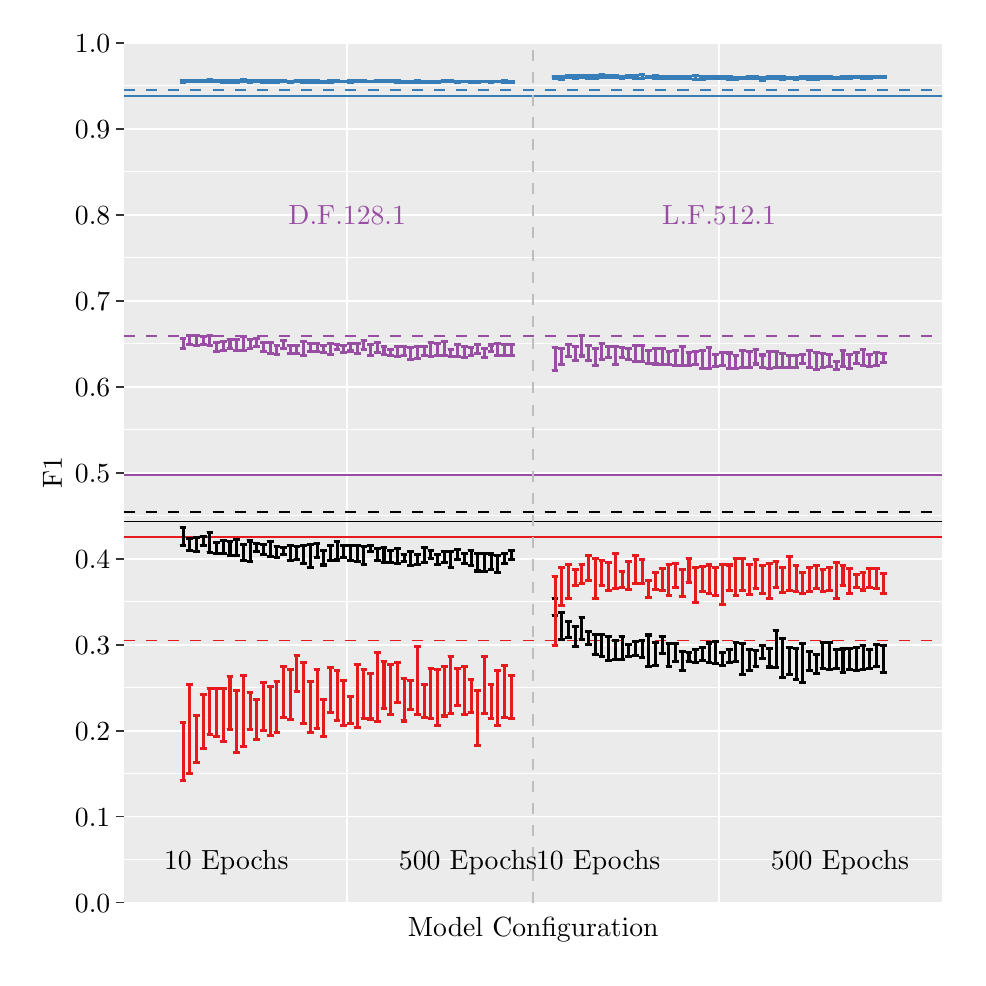
\begin{tikzpicture}[x=1pt,y=1pt]
\definecolor{fillColor}{RGB}{255,255,255}
\path[use as bounding box,fill=fillColor,fill opacity=0.00] (0,0) rectangle (336.00,336.00);
\begin{scope}
\path[clip] (  0.00,  0.00) rectangle (336.00,336.00);
\definecolor{drawColor}{RGB}{255,255,255}
\definecolor{fillColor}{RGB}{255,255,255}

\path[draw=drawColor,line width= 0.6pt,line join=round,line cap=round,fill=fillColor] (  0.00,  0.00) rectangle (336.00,336.00);
\end{scope}
\begin{scope}
\path[clip] ( 34.81, 19.83) rectangle (330.50,330.50);
\definecolor{fillColor}{gray}{0.92}

\path[fill=fillColor] ( 34.81, 19.83) rectangle (330.50,330.50);
\definecolor{drawColor}{RGB}{255,255,255}

\path[draw=drawColor,line width= 0.3pt,line join=round] ( 34.81, 35.36) --
	(330.50, 35.36);

\path[draw=drawColor,line width= 0.3pt,line join=round] ( 34.81, 66.43) --
	(330.50, 66.43);

\path[draw=drawColor,line width= 0.3pt,line join=round] ( 34.81, 97.50) --
	(330.50, 97.50);

\path[draw=drawColor,line width= 0.3pt,line join=round] ( 34.81,128.57) --
	(330.50,128.57);

\path[draw=drawColor,line width= 0.3pt,line join=round] ( 34.81,159.63) --
	(330.50,159.63);

\path[draw=drawColor,line width= 0.3pt,line join=round] ( 34.81,190.70) --
	(330.50,190.70);

\path[draw=drawColor,line width= 0.3pt,line join=round] ( 34.81,221.77) --
	(330.50,221.77);

\path[draw=drawColor,line width= 0.3pt,line join=round] ( 34.81,252.83) --
	(330.50,252.83);

\path[draw=drawColor,line width= 0.3pt,line join=round] ( 34.81,283.90) --
	(330.50,283.90);

\path[draw=drawColor,line width= 0.3pt,line join=round] ( 34.81,314.97) --
	(330.50,314.97);

\path[draw=drawColor,line width= 0.6pt,line join=round] ( 34.81, 19.83) --
	(330.50, 19.83);

\path[draw=drawColor,line width= 0.6pt,line join=round] ( 34.81, 50.90) --
	(330.50, 50.90);

\path[draw=drawColor,line width= 0.6pt,line join=round] ( 34.81, 81.96) --
	(330.50, 81.96);

\path[draw=drawColor,line width= 0.6pt,line join=round] ( 34.81,113.03) --
	(330.50,113.03);

\path[draw=drawColor,line width= 0.6pt,line join=round] ( 34.81,144.10) --
	(330.50,144.10);

\path[draw=drawColor,line width= 0.6pt,line join=round] ( 34.81,175.17) --
	(330.50,175.17);

\path[draw=drawColor,line width= 0.6pt,line join=round] ( 34.81,206.23) --
	(330.50,206.23);

\path[draw=drawColor,line width= 0.6pt,line join=round] ( 34.81,237.30) --
	(330.50,237.30);

\path[draw=drawColor,line width= 0.6pt,line join=round] ( 34.81,268.37) --
	(330.50,268.37);

\path[draw=drawColor,line width= 0.6pt,line join=round] ( 34.81,299.43) --
	(330.50,299.43);

\path[draw=drawColor,line width= 0.6pt,line join=round] ( 34.81,330.50) --
	(330.50,330.50);

\path[draw=drawColor,line width= 0.6pt,line join=round] (115.45, 19.83) --
	(115.45,330.50);

\path[draw=drawColor,line width= 0.6pt,line join=round] (249.86, 19.83) --
	(249.86,330.50);
\definecolor{drawColor}{RGB}{0,0,0}

\path[draw=drawColor,line width= 0.6pt,line join=round] ( 34.81,157.51) -- (330.50,157.51);
\definecolor{drawColor}{RGB}{55,126,184}

\path[draw=drawColor,line width= 0.6pt,line join=round] ( 34.81,311.32) -- (330.50,311.32);
\definecolor{drawColor}{RGB}{228,26,28}

\path[draw=drawColor,line width= 0.6pt,line join=round] ( 34.81,152.03) -- (330.50,152.03);
\definecolor{drawColor}{RGB}{152,78,163}

\path[draw=drawColor,line width= 0.6pt,line join=round] ( 34.81,174.40) -- (330.50,174.40);
\definecolor{drawColor}{RGB}{0,0,0}

\path[draw=drawColor,line width= 0.6pt,dash pattern=on 4pt off 4pt ,line join=round] ( 34.81,160.94) -- (330.50,160.94);
\definecolor{drawColor}{RGB}{55,126,184}

\path[draw=drawColor,line width= 0.6pt,dash pattern=on 4pt off 4pt ,line join=round] ( 34.81,313.44) -- (330.50,313.44);
\definecolor{drawColor}{RGB}{228,26,28}

\path[draw=drawColor,line width= 0.6pt,dash pattern=on 4pt off 4pt ,line join=round] ( 34.81,114.54) -- (330.50,114.54);
\definecolor{drawColor}{RGB}{152,78,163}

\path[draw=drawColor,line width= 0.6pt,dash pattern=on 4pt off 4pt ,line join=round] ( 34.81,224.68) -- (330.50,224.68);
\definecolor{drawColor}{RGB}{190,190,190}

\path[draw=drawColor,line width= 0.6pt,dash pattern=on 4pt off 4pt ,line join=round] (182.65, 19.83) -- (182.65,330.50);
\definecolor{drawColor}{RGB}{0,0,0}

\path[draw=drawColor,line width= 1.1pt,line join=round] (173.51,147.01) --
	(175.93,147.01);

\path[draw=drawColor,line width= 1.1pt,line join=round] (174.72,147.01) --
	(174.72,143.94);

\path[draw=drawColor,line width= 1.1pt,line join=round] (173.51,143.94) --
	(175.93,143.94);

\path[draw=drawColor,line width= 1.1pt,line join=round] (173.51,147.01) --
	(175.93,147.01);

\path[draw=drawColor,line width= 1.1pt,line join=round] (174.72,147.01) --
	(174.72,143.94);

\path[draw=drawColor,line width= 1.1pt,line join=round] (173.51,143.94) --
	(175.93,143.94);

\path[draw=drawColor,line width= 1.1pt,line join=round] (173.51,147.01) --
	(175.93,147.01);

\path[draw=drawColor,line width= 1.1pt,line join=round] (174.72,147.01) --
	(174.72,143.94);

\path[draw=drawColor,line width= 1.1pt,line join=round] (173.51,143.94) --
	(175.93,143.94);

\path[draw=drawColor,line width= 1.1pt,line join=round] (173.51,147.01) --
	(175.93,147.01);

\path[draw=drawColor,line width= 1.1pt,line join=round] (174.72,147.01) --
	(174.72,143.94);

\path[draw=drawColor,line width= 1.1pt,line join=round] (173.51,143.94) --
	(175.93,143.94);

\path[draw=drawColor,line width= 1.1pt,line join=round] (173.51,147.01) --
	(175.93,147.01);

\path[draw=drawColor,line width= 1.1pt,line join=round] (174.72,147.01) --
	(174.72,143.94);

\path[draw=drawColor,line width= 1.1pt,line join=round] (173.51,143.94) --
	(175.93,143.94);

\path[draw=drawColor,line width= 1.1pt,line join=round] (173.51,147.01) --
	(175.93,147.01);

\path[draw=drawColor,line width= 1.1pt,line join=round] (174.72,147.01) --
	(174.72,143.94);

\path[draw=drawColor,line width= 1.1pt,line join=round] (173.51,143.94) --
	(175.93,143.94);

\path[draw=drawColor,line width= 1.1pt,line join=round] (173.51,147.01) --
	(175.93,147.01);

\path[draw=drawColor,line width= 1.1pt,line join=round] (174.72,147.01) --
	(174.72,143.94);

\path[draw=drawColor,line width= 1.1pt,line join=round] (173.51,143.94) --
	(175.93,143.94);

\path[draw=drawColor,line width= 1.1pt,line join=round] (173.51,147.01) --
	(175.93,147.01);

\path[draw=drawColor,line width= 1.1pt,line join=round] (174.72,147.01) --
	(174.72,143.94);

\path[draw=drawColor,line width= 1.1pt,line join=round] (173.51,143.94) --
	(175.93,143.94);

\path[draw=drawColor,line width= 1.1pt,line join=round] (171.09,145.88) --
	(173.51,145.88);

\path[draw=drawColor,line width= 1.1pt,line join=round] (172.30,145.88) --
	(172.30,142.48);

\path[draw=drawColor,line width= 1.1pt,line join=round] (171.09,142.48) --
	(173.51,142.48);

\path[draw=drawColor,line width= 1.1pt,line join=round] (171.09,145.88) --
	(173.51,145.88);

\path[draw=drawColor,line width= 1.1pt,line join=round] (172.30,145.88) --
	(172.30,142.48);

\path[draw=drawColor,line width= 1.1pt,line join=round] (171.09,142.48) --
	(173.51,142.48);

\path[draw=drawColor,line width= 1.1pt,line join=round] (171.09,145.88) --
	(173.51,145.88);

\path[draw=drawColor,line width= 1.1pt,line join=round] (172.30,145.88) --
	(172.30,142.48);

\path[draw=drawColor,line width= 1.1pt,line join=round] (171.09,142.48) --
	(173.51,142.48);

\path[draw=drawColor,line width= 1.1pt,line join=round] (171.09,145.88) --
	(173.51,145.88);

\path[draw=drawColor,line width= 1.1pt,line join=round] (172.30,145.88) --
	(172.30,142.48);

\path[draw=drawColor,line width= 1.1pt,line join=round] (171.09,142.48) --
	(173.51,142.48);

\path[draw=drawColor,line width= 1.1pt,line join=round] (171.09,145.88) --
	(173.51,145.88);

\path[draw=drawColor,line width= 1.1pt,line join=round] (172.30,145.88) --
	(172.30,142.48);

\path[draw=drawColor,line width= 1.1pt,line join=round] (171.09,142.48) --
	(173.51,142.48);

\path[draw=drawColor,line width= 1.1pt,line join=round] (171.09,145.88) --
	(173.51,145.88);

\path[draw=drawColor,line width= 1.1pt,line join=round] (172.30,145.88) --
	(172.30,142.48);

\path[draw=drawColor,line width= 1.1pt,line join=round] (171.09,142.48) --
	(173.51,142.48);

\path[draw=drawColor,line width= 1.1pt,line join=round] (171.09,145.88) --
	(173.51,145.88);

\path[draw=drawColor,line width= 1.1pt,line join=round] (172.30,145.88) --
	(172.30,142.48);

\path[draw=drawColor,line width= 1.1pt,line join=round] (171.09,142.48) --
	(173.51,142.48);

\path[draw=drawColor,line width= 1.1pt,line join=round] (171.09,145.88) --
	(173.51,145.88);

\path[draw=drawColor,line width= 1.1pt,line join=round] (172.30,145.88) --
	(172.30,142.48);

\path[draw=drawColor,line width= 1.1pt,line join=round] (171.09,142.48) --
	(173.51,142.48);

\path[draw=drawColor,line width= 1.1pt,line join=round] (168.67,145.20) --
	(171.09,145.20);

\path[draw=drawColor,line width= 1.1pt,line join=round] (169.88,145.20) --
	(169.88,139.00);

\path[draw=drawColor,line width= 1.1pt,line join=round] (168.67,139.00) --
	(171.09,139.00);

\path[draw=drawColor,line width= 1.1pt,line join=round] (168.67,145.20) --
	(171.09,145.20);

\path[draw=drawColor,line width= 1.1pt,line join=round] (169.88,145.20) --
	(169.88,139.00);

\path[draw=drawColor,line width= 1.1pt,line join=round] (168.67,139.00) --
	(171.09,139.00);

\path[draw=drawColor,line width= 1.1pt,line join=round] (168.67,145.20) --
	(171.09,145.20);

\path[draw=drawColor,line width= 1.1pt,line join=round] (169.88,145.20) --
	(169.88,139.00);

\path[draw=drawColor,line width= 1.1pt,line join=round] (168.67,139.00) --
	(171.09,139.00);

\path[draw=drawColor,line width= 1.1pt,line join=round] (168.67,145.20) --
	(171.09,145.20);

\path[draw=drawColor,line width= 1.1pt,line join=round] (169.88,145.20) --
	(169.88,139.00);

\path[draw=drawColor,line width= 1.1pt,line join=round] (168.67,139.00) --
	(171.09,139.00);

\path[draw=drawColor,line width= 1.1pt,line join=round] (168.67,145.20) --
	(171.09,145.20);

\path[draw=drawColor,line width= 1.1pt,line join=round] (169.88,145.20) --
	(169.88,139.00);

\path[draw=drawColor,line width= 1.1pt,line join=round] (168.67,139.00) --
	(171.09,139.00);

\path[draw=drawColor,line width= 1.1pt,line join=round] (168.67,145.20) --
	(171.09,145.20);

\path[draw=drawColor,line width= 1.1pt,line join=round] (169.88,145.20) --
	(169.88,139.00);

\path[draw=drawColor,line width= 1.1pt,line join=round] (168.67,139.00) --
	(171.09,139.00);

\path[draw=drawColor,line width= 1.1pt,line join=round] (168.67,145.20) --
	(171.09,145.20);

\path[draw=drawColor,line width= 1.1pt,line join=round] (169.88,145.20) --
	(169.88,139.00);

\path[draw=drawColor,line width= 1.1pt,line join=round] (168.67,139.00) --
	(171.09,139.00);

\path[draw=drawColor,line width= 1.1pt,line join=round] (168.67,145.20) --
	(171.09,145.20);

\path[draw=drawColor,line width= 1.1pt,line join=round] (169.88,145.20) --
	(169.88,139.00);

\path[draw=drawColor,line width= 1.1pt,line join=round] (168.67,139.00) --
	(171.09,139.00);

\path[draw=drawColor,line width= 1.1pt,line join=round] (166.26,145.81) --
	(168.67,145.81);

\path[draw=drawColor,line width= 1.1pt,line join=round] (167.46,145.81) --
	(167.46,140.18);

\path[draw=drawColor,line width= 1.1pt,line join=round] (166.26,140.18) --
	(168.67,140.18);

\path[draw=drawColor,line width= 1.1pt,line join=round] (166.26,145.81) --
	(168.67,145.81);

\path[draw=drawColor,line width= 1.1pt,line join=round] (167.46,145.81) --
	(167.46,140.18);

\path[draw=drawColor,line width= 1.1pt,line join=round] (166.26,140.18) --
	(168.67,140.18);

\path[draw=drawColor,line width= 1.1pt,line join=round] (166.26,145.81) --
	(168.67,145.81);

\path[draw=drawColor,line width= 1.1pt,line join=round] (167.46,145.81) --
	(167.46,140.18);

\path[draw=drawColor,line width= 1.1pt,line join=round] (166.26,140.18) --
	(168.67,140.18);

\path[draw=drawColor,line width= 1.1pt,line join=round] (166.26,145.81) --
	(168.67,145.81);

\path[draw=drawColor,line width= 1.1pt,line join=round] (167.46,145.81) --
	(167.46,140.18);

\path[draw=drawColor,line width= 1.1pt,line join=round] (166.26,140.18) --
	(168.67,140.18);

\path[draw=drawColor,line width= 1.1pt,line join=round] (166.26,145.81) --
	(168.67,145.81);

\path[draw=drawColor,line width= 1.1pt,line join=round] (167.46,145.81) --
	(167.46,140.18);

\path[draw=drawColor,line width= 1.1pt,line join=round] (166.26,140.18) --
	(168.67,140.18);

\path[draw=drawColor,line width= 1.1pt,line join=round] (166.26,145.81) --
	(168.67,145.81);

\path[draw=drawColor,line width= 1.1pt,line join=round] (167.46,145.81) --
	(167.46,140.18);

\path[draw=drawColor,line width= 1.1pt,line join=round] (166.26,140.18) --
	(168.67,140.18);

\path[draw=drawColor,line width= 1.1pt,line join=round] (166.26,145.81) --
	(168.67,145.81);

\path[draw=drawColor,line width= 1.1pt,line join=round] (167.46,145.81) --
	(167.46,140.18);

\path[draw=drawColor,line width= 1.1pt,line join=round] (166.26,140.18) --
	(168.67,140.18);

\path[draw=drawColor,line width= 1.1pt,line join=round] (166.26,145.81) --
	(168.67,145.81);

\path[draw=drawColor,line width= 1.1pt,line join=round] (167.46,145.81) --
	(167.46,140.18);

\path[draw=drawColor,line width= 1.1pt,line join=round] (166.26,140.18) --
	(168.67,140.18);

\path[draw=drawColor,line width= 1.1pt,line join=round] (163.84,146.09) --
	(166.26,146.09);

\path[draw=drawColor,line width= 1.1pt,line join=round] (165.05,146.09) --
	(165.05,139.37);

\path[draw=drawColor,line width= 1.1pt,line join=round] (163.84,139.37) --
	(166.26,139.37);

\path[draw=drawColor,line width= 1.1pt,line join=round] (163.84,146.09) --
	(166.26,146.09);

\path[draw=drawColor,line width= 1.1pt,line join=round] (165.05,146.09) --
	(165.05,139.37);

\path[draw=drawColor,line width= 1.1pt,line join=round] (163.84,139.37) --
	(166.26,139.37);

\path[draw=drawColor,line width= 1.1pt,line join=round] (163.84,146.09) --
	(166.26,146.09);

\path[draw=drawColor,line width= 1.1pt,line join=round] (165.05,146.09) --
	(165.05,139.37);

\path[draw=drawColor,line width= 1.1pt,line join=round] (163.84,139.37) --
	(166.26,139.37);

\path[draw=drawColor,line width= 1.1pt,line join=round] (163.84,146.09) --
	(166.26,146.09);

\path[draw=drawColor,line width= 1.1pt,line join=round] (165.05,146.09) --
	(165.05,139.37);

\path[draw=drawColor,line width= 1.1pt,line join=round] (163.84,139.37) --
	(166.26,139.37);

\path[draw=drawColor,line width= 1.1pt,line join=round] (163.84,146.09) --
	(166.26,146.09);

\path[draw=drawColor,line width= 1.1pt,line join=round] (165.05,146.09) --
	(165.05,139.37);

\path[draw=drawColor,line width= 1.1pt,line join=round] (163.84,139.37) --
	(166.26,139.37);

\path[draw=drawColor,line width= 1.1pt,line join=round] (163.84,146.09) --
	(166.26,146.09);

\path[draw=drawColor,line width= 1.1pt,line join=round] (165.05,146.09) --
	(165.05,139.37);

\path[draw=drawColor,line width= 1.1pt,line join=round] (163.84,139.37) --
	(166.26,139.37);

\path[draw=drawColor,line width= 1.1pt,line join=round] (163.84,146.09) --
	(166.26,146.09);

\path[draw=drawColor,line width= 1.1pt,line join=round] (165.05,146.09) --
	(165.05,139.37);

\path[draw=drawColor,line width= 1.1pt,line join=round] (163.84,139.37) --
	(166.26,139.37);

\path[draw=drawColor,line width= 1.1pt,line join=round] (163.84,146.09) --
	(166.26,146.09);

\path[draw=drawColor,line width= 1.1pt,line join=round] (165.05,146.09) --
	(165.05,139.37);

\path[draw=drawColor,line width= 1.1pt,line join=round] (163.84,139.37) --
	(166.26,139.37);

\path[draw=drawColor,line width= 1.1pt,line join=round] (161.42,145.88) --
	(163.84,145.88);

\path[draw=drawColor,line width= 1.1pt,line join=round] (162.63,145.88) --
	(162.63,139.67);

\path[draw=drawColor,line width= 1.1pt,line join=round] (161.42,139.67) --
	(163.84,139.67);

\path[draw=drawColor,line width= 1.1pt,line join=round] (161.42,145.88) --
	(163.84,145.88);

\path[draw=drawColor,line width= 1.1pt,line join=round] (162.63,145.88) --
	(162.63,139.67);

\path[draw=drawColor,line width= 1.1pt,line join=round] (161.42,139.67) --
	(163.84,139.67);

\path[draw=drawColor,line width= 1.1pt,line join=round] (161.42,145.88) --
	(163.84,145.88);

\path[draw=drawColor,line width= 1.1pt,line join=round] (162.63,145.88) --
	(162.63,139.67);

\path[draw=drawColor,line width= 1.1pt,line join=round] (161.42,139.67) --
	(163.84,139.67);

\path[draw=drawColor,line width= 1.1pt,line join=round] (161.42,145.88) --
	(163.84,145.88);

\path[draw=drawColor,line width= 1.1pt,line join=round] (162.63,145.88) --
	(162.63,139.67);

\path[draw=drawColor,line width= 1.1pt,line join=round] (161.42,139.67) --
	(163.84,139.67);

\path[draw=drawColor,line width= 1.1pt,line join=round] (161.42,145.88) --
	(163.84,145.88);

\path[draw=drawColor,line width= 1.1pt,line join=round] (162.63,145.88) --
	(162.63,139.67);

\path[draw=drawColor,line width= 1.1pt,line join=round] (161.42,139.67) --
	(163.84,139.67);

\path[draw=drawColor,line width= 1.1pt,line join=round] (161.42,145.88) --
	(163.84,145.88);

\path[draw=drawColor,line width= 1.1pt,line join=round] (162.63,145.88) --
	(162.63,139.67);

\path[draw=drawColor,line width= 1.1pt,line join=round] (161.42,139.67) --
	(163.84,139.67);

\path[draw=drawColor,line width= 1.1pt,line join=round] (161.42,145.88) --
	(163.84,145.88);

\path[draw=drawColor,line width= 1.1pt,line join=round] (162.63,145.88) --
	(162.63,139.67);

\path[draw=drawColor,line width= 1.1pt,line join=round] (161.42,139.67) --
	(163.84,139.67);

\path[draw=drawColor,line width= 1.1pt,line join=round] (161.42,145.88) --
	(163.84,145.88);

\path[draw=drawColor,line width= 1.1pt,line join=round] (162.63,145.88) --
	(162.63,139.67);

\path[draw=drawColor,line width= 1.1pt,line join=round] (161.42,139.67) --
	(163.84,139.67);

\path[draw=drawColor,line width= 1.1pt,line join=round] (159.00,147.08) --
	(161.42,147.08);

\path[draw=drawColor,line width= 1.1pt,line join=round] (160.21,147.08) --
	(160.21,141.58);

\path[draw=drawColor,line width= 1.1pt,line join=round] (159.00,141.58) --
	(161.42,141.58);

\path[draw=drawColor,line width= 1.1pt,line join=round] (159.00,147.08) --
	(161.42,147.08);

\path[draw=drawColor,line width= 1.1pt,line join=round] (160.21,147.08) --
	(160.21,141.58);

\path[draw=drawColor,line width= 1.1pt,line join=round] (159.00,141.58) --
	(161.42,141.58);

\path[draw=drawColor,line width= 1.1pt,line join=round] (159.00,147.08) --
	(161.42,147.08);

\path[draw=drawColor,line width= 1.1pt,line join=round] (160.21,147.08) --
	(160.21,141.58);

\path[draw=drawColor,line width= 1.1pt,line join=round] (159.00,141.58) --
	(161.42,141.58);

\path[draw=drawColor,line width= 1.1pt,line join=round] (159.00,147.08) --
	(161.42,147.08);

\path[draw=drawColor,line width= 1.1pt,line join=round] (160.21,147.08) --
	(160.21,141.58);

\path[draw=drawColor,line width= 1.1pt,line join=round] (159.00,141.58) --
	(161.42,141.58);

\path[draw=drawColor,line width= 1.1pt,line join=round] (159.00,147.08) --
	(161.42,147.08);

\path[draw=drawColor,line width= 1.1pt,line join=round] (160.21,147.08) --
	(160.21,141.58);

\path[draw=drawColor,line width= 1.1pt,line join=round] (159.00,141.58) --
	(161.42,141.58);

\path[draw=drawColor,line width= 1.1pt,line join=round] (159.00,147.08) --
	(161.42,147.08);

\path[draw=drawColor,line width= 1.1pt,line join=round] (160.21,147.08) --
	(160.21,141.58);

\path[draw=drawColor,line width= 1.1pt,line join=round] (159.00,141.58) --
	(161.42,141.58);

\path[draw=drawColor,line width= 1.1pt,line join=round] (159.00,147.08) --
	(161.42,147.08);

\path[draw=drawColor,line width= 1.1pt,line join=round] (160.21,147.08) --
	(160.21,141.58);

\path[draw=drawColor,line width= 1.1pt,line join=round] (159.00,141.58) --
	(161.42,141.58);

\path[draw=drawColor,line width= 1.1pt,line join=round] (159.00,147.08) --
	(161.42,147.08);

\path[draw=drawColor,line width= 1.1pt,line join=round] (160.21,147.08) --
	(160.21,141.58);

\path[draw=drawColor,line width= 1.1pt,line join=round] (159.00,141.58) --
	(161.42,141.58);

\path[draw=drawColor,line width= 1.1pt,line join=round] (156.58,146.00) --
	(159.00,146.00);

\path[draw=drawColor,line width= 1.1pt,line join=round] (157.79,146.00) --
	(157.79,142.24);

\path[draw=drawColor,line width= 1.1pt,line join=round] (156.58,142.24) --
	(159.00,142.24);

\path[draw=drawColor,line width= 1.1pt,line join=round] (156.58,146.00) --
	(159.00,146.00);

\path[draw=drawColor,line width= 1.1pt,line join=round] (157.79,146.00) --
	(157.79,142.24);

\path[draw=drawColor,line width= 1.1pt,line join=round] (156.58,142.24) --
	(159.00,142.24);

\path[draw=drawColor,line width= 1.1pt,line join=round] (156.58,146.00) --
	(159.00,146.00);

\path[draw=drawColor,line width= 1.1pt,line join=round] (157.79,146.00) --
	(157.79,142.24);

\path[draw=drawColor,line width= 1.1pt,line join=round] (156.58,142.24) --
	(159.00,142.24);

\path[draw=drawColor,line width= 1.1pt,line join=round] (156.58,146.00) --
	(159.00,146.00);

\path[draw=drawColor,line width= 1.1pt,line join=round] (157.79,146.00) --
	(157.79,142.24);

\path[draw=drawColor,line width= 1.1pt,line join=round] (156.58,142.24) --
	(159.00,142.24);

\path[draw=drawColor,line width= 1.1pt,line join=round] (156.58,146.00) --
	(159.00,146.00);

\path[draw=drawColor,line width= 1.1pt,line join=round] (157.79,146.00) --
	(157.79,142.24);

\path[draw=drawColor,line width= 1.1pt,line join=round] (156.58,142.24) --
	(159.00,142.24);

\path[draw=drawColor,line width= 1.1pt,line join=round] (156.58,146.00) --
	(159.00,146.00);

\path[draw=drawColor,line width= 1.1pt,line join=round] (157.79,146.00) --
	(157.79,142.24);

\path[draw=drawColor,line width= 1.1pt,line join=round] (156.58,142.24) --
	(159.00,142.24);

\path[draw=drawColor,line width= 1.1pt,line join=round] (156.58,146.00) --
	(159.00,146.00);

\path[draw=drawColor,line width= 1.1pt,line join=round] (157.79,146.00) --
	(157.79,142.24);

\path[draw=drawColor,line width= 1.1pt,line join=round] (156.58,142.24) --
	(159.00,142.24);

\path[draw=drawColor,line width= 1.1pt,line join=round] (156.58,146.00) --
	(159.00,146.00);

\path[draw=drawColor,line width= 1.1pt,line join=round] (157.79,146.00) --
	(157.79,142.24);

\path[draw=drawColor,line width= 1.1pt,line join=round] (156.58,142.24) --
	(159.00,142.24);

\path[draw=drawColor,line width= 1.1pt,line join=round] (154.16,147.31) --
	(156.58,147.31);

\path[draw=drawColor,line width= 1.1pt,line join=round] (155.37,147.31) --
	(155.37,143.92);

\path[draw=drawColor,line width= 1.1pt,line join=round] (154.16,143.92) --
	(156.58,143.92);

\path[draw=drawColor,line width= 1.1pt,line join=round] (154.16,147.31) --
	(156.58,147.31);

\path[draw=drawColor,line width= 1.1pt,line join=round] (155.37,147.31) --
	(155.37,143.92);

\path[draw=drawColor,line width= 1.1pt,line join=round] (154.16,143.92) --
	(156.58,143.92);

\path[draw=drawColor,line width= 1.1pt,line join=round] (154.16,147.31) --
	(156.58,147.31);

\path[draw=drawColor,line width= 1.1pt,line join=round] (155.37,147.31) --
	(155.37,143.92);

\path[draw=drawColor,line width= 1.1pt,line join=round] (154.16,143.92) --
	(156.58,143.92);

\path[draw=drawColor,line width= 1.1pt,line join=round] (154.16,147.31) --
	(156.58,147.31);

\path[draw=drawColor,line width= 1.1pt,line join=round] (155.37,147.31) --
	(155.37,143.92);

\path[draw=drawColor,line width= 1.1pt,line join=round] (154.16,143.92) --
	(156.58,143.92);

\path[draw=drawColor,line width= 1.1pt,line join=round] (154.16,147.31) --
	(156.58,147.31);

\path[draw=drawColor,line width= 1.1pt,line join=round] (155.37,147.31) --
	(155.37,143.92);

\path[draw=drawColor,line width= 1.1pt,line join=round] (154.16,143.92) --
	(156.58,143.92);

\path[draw=drawColor,line width= 1.1pt,line join=round] (154.16,147.31) --
	(156.58,147.31);

\path[draw=drawColor,line width= 1.1pt,line join=round] (155.37,147.31) --
	(155.37,143.92);

\path[draw=drawColor,line width= 1.1pt,line join=round] (154.16,143.92) --
	(156.58,143.92);

\path[draw=drawColor,line width= 1.1pt,line join=round] (154.16,147.31) --
	(156.58,147.31);

\path[draw=drawColor,line width= 1.1pt,line join=round] (155.37,147.31) --
	(155.37,143.92);

\path[draw=drawColor,line width= 1.1pt,line join=round] (154.16,143.92) --
	(156.58,143.92);

\path[draw=drawColor,line width= 1.1pt,line join=round] (154.16,147.31) --
	(156.58,147.31);

\path[draw=drawColor,line width= 1.1pt,line join=round] (155.37,147.31) --
	(155.37,143.92);

\path[draw=drawColor,line width= 1.1pt,line join=round] (154.16,143.92) --
	(156.58,143.92);

\path[draw=drawColor,line width= 1.1pt,line join=round] (151.74,146.73) --
	(154.16,146.73);

\path[draw=drawColor,line width= 1.1pt,line join=round] (152.95,146.73) --
	(152.95,140.78);

\path[draw=drawColor,line width= 1.1pt,line join=round] (151.74,140.78) --
	(154.16,140.78);

\path[draw=drawColor,line width= 1.1pt,line join=round] (151.74,146.73) --
	(154.16,146.73);

\path[draw=drawColor,line width= 1.1pt,line join=round] (152.95,146.73) --
	(152.95,140.78);

\path[draw=drawColor,line width= 1.1pt,line join=round] (151.74,140.78) --
	(154.16,140.78);

\path[draw=drawColor,line width= 1.1pt,line join=round] (151.74,146.73) --
	(154.16,146.73);

\path[draw=drawColor,line width= 1.1pt,line join=round] (152.95,146.73) --
	(152.95,140.78);

\path[draw=drawColor,line width= 1.1pt,line join=round] (151.74,140.78) --
	(154.16,140.78);

\path[draw=drawColor,line width= 1.1pt,line join=round] (151.74,146.73) --
	(154.16,146.73);

\path[draw=drawColor,line width= 1.1pt,line join=round] (152.95,146.73) --
	(152.95,140.78);

\path[draw=drawColor,line width= 1.1pt,line join=round] (151.74,140.78) --
	(154.16,140.78);

\path[draw=drawColor,line width= 1.1pt,line join=round] (151.74,146.73) --
	(154.16,146.73);

\path[draw=drawColor,line width= 1.1pt,line join=round] (152.95,146.73) --
	(152.95,140.78);

\path[draw=drawColor,line width= 1.1pt,line join=round] (151.74,140.78) --
	(154.16,140.78);

\path[draw=drawColor,line width= 1.1pt,line join=round] (151.74,146.73) --
	(154.16,146.73);

\path[draw=drawColor,line width= 1.1pt,line join=round] (152.95,146.73) --
	(152.95,140.78);

\path[draw=drawColor,line width= 1.1pt,line join=round] (151.74,140.78) --
	(154.16,140.78);

\path[draw=drawColor,line width= 1.1pt,line join=round] (151.74,146.73) --
	(154.16,146.73);

\path[draw=drawColor,line width= 1.1pt,line join=round] (152.95,146.73) --
	(152.95,140.78);

\path[draw=drawColor,line width= 1.1pt,line join=round] (151.74,140.78) --
	(154.16,140.78);

\path[draw=drawColor,line width= 1.1pt,line join=round] (151.74,146.73) --
	(154.16,146.73);

\path[draw=drawColor,line width= 1.1pt,line join=round] (152.95,146.73) --
	(152.95,140.78);

\path[draw=drawColor,line width= 1.1pt,line join=round] (151.74,140.78) --
	(154.16,140.78);

\path[draw=drawColor,line width= 1.1pt,line join=round] (149.32,146.57) --
	(151.74,146.57);

\path[draw=drawColor,line width= 1.1pt,line join=round] (150.53,146.57) --
	(150.53,142.76);

\path[draw=drawColor,line width= 1.1pt,line join=round] (149.32,142.76) --
	(151.74,142.76);

\path[draw=drawColor,line width= 1.1pt,line join=round] (149.32,146.57) --
	(151.74,146.57);

\path[draw=drawColor,line width= 1.1pt,line join=round] (150.53,146.57) --
	(150.53,142.76);

\path[draw=drawColor,line width= 1.1pt,line join=round] (149.32,142.76) --
	(151.74,142.76);

\path[draw=drawColor,line width= 1.1pt,line join=round] (149.32,146.57) --
	(151.74,146.57);

\path[draw=drawColor,line width= 1.1pt,line join=round] (150.53,146.57) --
	(150.53,142.76);

\path[draw=drawColor,line width= 1.1pt,line join=round] (149.32,142.76) --
	(151.74,142.76);

\path[draw=drawColor,line width= 1.1pt,line join=round] (149.32,146.57) --
	(151.74,146.57);

\path[draw=drawColor,line width= 1.1pt,line join=round] (150.53,146.57) --
	(150.53,142.76);

\path[draw=drawColor,line width= 1.1pt,line join=round] (149.32,142.76) --
	(151.74,142.76);

\path[draw=drawColor,line width= 1.1pt,line join=round] (149.32,146.57) --
	(151.74,146.57);

\path[draw=drawColor,line width= 1.1pt,line join=round] (150.53,146.57) --
	(150.53,142.76);

\path[draw=drawColor,line width= 1.1pt,line join=round] (149.32,142.76) --
	(151.74,142.76);

\path[draw=drawColor,line width= 1.1pt,line join=round] (149.32,146.57) --
	(151.74,146.57);

\path[draw=drawColor,line width= 1.1pt,line join=round] (150.53,146.57) --
	(150.53,142.76);

\path[draw=drawColor,line width= 1.1pt,line join=round] (149.32,142.76) --
	(151.74,142.76);

\path[draw=drawColor,line width= 1.1pt,line join=round] (149.32,146.57) --
	(151.74,146.57);

\path[draw=drawColor,line width= 1.1pt,line join=round] (150.53,146.57) --
	(150.53,142.76);

\path[draw=drawColor,line width= 1.1pt,line join=round] (149.32,142.76) --
	(151.74,142.76);

\path[draw=drawColor,line width= 1.1pt,line join=round] (149.32,146.57) --
	(151.74,146.57);

\path[draw=drawColor,line width= 1.1pt,line join=round] (150.53,146.57) --
	(150.53,142.76);

\path[draw=drawColor,line width= 1.1pt,line join=round] (149.32,142.76) --
	(151.74,142.76);

\path[draw=drawColor,line width= 1.1pt,line join=round] (146.90,145.61) --
	(149.32,145.61);

\path[draw=drawColor,line width= 1.1pt,line join=round] (148.11,145.61) --
	(148.11,141.94);

\path[draw=drawColor,line width= 1.1pt,line join=round] (146.90,141.94) --
	(149.32,141.94);

\path[draw=drawColor,line width= 1.1pt,line join=round] (146.90,145.61) --
	(149.32,145.61);

\path[draw=drawColor,line width= 1.1pt,line join=round] (148.11,145.61) --
	(148.11,141.94);

\path[draw=drawColor,line width= 1.1pt,line join=round] (146.90,141.94) --
	(149.32,141.94);

\path[draw=drawColor,line width= 1.1pt,line join=round] (146.90,145.61) --
	(149.32,145.61);

\path[draw=drawColor,line width= 1.1pt,line join=round] (148.11,145.61) --
	(148.11,141.94);

\path[draw=drawColor,line width= 1.1pt,line join=round] (146.90,141.94) --
	(149.32,141.94);

\path[draw=drawColor,line width= 1.1pt,line join=round] (146.90,145.61) --
	(149.32,145.61);

\path[draw=drawColor,line width= 1.1pt,line join=round] (148.11,145.61) --
	(148.11,141.94);

\path[draw=drawColor,line width= 1.1pt,line join=round] (146.90,141.94) --
	(149.32,141.94);

\path[draw=drawColor,line width= 1.1pt,line join=round] (146.90,145.61) --
	(149.32,145.61);

\path[draw=drawColor,line width= 1.1pt,line join=round] (148.11,145.61) --
	(148.11,141.94);

\path[draw=drawColor,line width= 1.1pt,line join=round] (146.90,141.94) --
	(149.32,141.94);

\path[draw=drawColor,line width= 1.1pt,line join=round] (146.90,145.61) --
	(149.32,145.61);

\path[draw=drawColor,line width= 1.1pt,line join=round] (148.11,145.61) --
	(148.11,141.94);

\path[draw=drawColor,line width= 1.1pt,line join=round] (146.90,141.94) --
	(149.32,141.94);

\path[draw=drawColor,line width= 1.1pt,line join=round] (146.90,145.61) --
	(149.32,145.61);

\path[draw=drawColor,line width= 1.1pt,line join=round] (148.11,145.61) --
	(148.11,141.94);

\path[draw=drawColor,line width= 1.1pt,line join=round] (146.90,141.94) --
	(149.32,141.94);

\path[draw=drawColor,line width= 1.1pt,line join=round] (146.90,145.61) --
	(149.32,145.61);

\path[draw=drawColor,line width= 1.1pt,line join=round] (148.11,145.61) --
	(148.11,141.94);

\path[draw=drawColor,line width= 1.1pt,line join=round] (146.90,141.94) --
	(149.32,141.94);

\path[draw=drawColor,line width= 1.1pt,line join=round] (144.48,147.13) --
	(146.90,147.13);

\path[draw=drawColor,line width= 1.1pt,line join=round] (145.69,147.13) --
	(145.69,144.16);

\path[draw=drawColor,line width= 1.1pt,line join=round] (144.48,144.16) --
	(146.90,144.16);

\path[draw=drawColor,line width= 1.1pt,line join=round] (144.48,147.13) --
	(146.90,147.13);

\path[draw=drawColor,line width= 1.1pt,line join=round] (145.69,147.13) --
	(145.69,144.16);

\path[draw=drawColor,line width= 1.1pt,line join=round] (144.48,144.16) --
	(146.90,144.16);

\path[draw=drawColor,line width= 1.1pt,line join=round] (144.48,147.13) --
	(146.90,147.13);

\path[draw=drawColor,line width= 1.1pt,line join=round] (145.69,147.13) --
	(145.69,144.16);

\path[draw=drawColor,line width= 1.1pt,line join=round] (144.48,144.16) --
	(146.90,144.16);

\path[draw=drawColor,line width= 1.1pt,line join=round] (144.48,147.13) --
	(146.90,147.13);

\path[draw=drawColor,line width= 1.1pt,line join=round] (145.69,147.13) --
	(145.69,144.16);

\path[draw=drawColor,line width= 1.1pt,line join=round] (144.48,144.16) --
	(146.90,144.16);

\path[draw=drawColor,line width= 1.1pt,line join=round] (144.48,147.13) --
	(146.90,147.13);

\path[draw=drawColor,line width= 1.1pt,line join=round] (145.69,147.13) --
	(145.69,144.16);

\path[draw=drawColor,line width= 1.1pt,line join=round] (144.48,144.16) --
	(146.90,144.16);

\path[draw=drawColor,line width= 1.1pt,line join=round] (144.48,147.13) --
	(146.90,147.13);

\path[draw=drawColor,line width= 1.1pt,line join=round] (145.69,147.13) --
	(145.69,144.16);

\path[draw=drawColor,line width= 1.1pt,line join=round] (144.48,144.16) --
	(146.90,144.16);

\path[draw=drawColor,line width= 1.1pt,line join=round] (144.48,147.13) --
	(146.90,147.13);

\path[draw=drawColor,line width= 1.1pt,line join=round] (145.69,147.13) --
	(145.69,144.16);

\path[draw=drawColor,line width= 1.1pt,line join=round] (144.48,144.16) --
	(146.90,144.16);

\path[draw=drawColor,line width= 1.1pt,line join=round] (144.48,147.13) --
	(146.90,147.13);

\path[draw=drawColor,line width= 1.1pt,line join=round] (145.69,147.13) --
	(145.69,144.16);

\path[draw=drawColor,line width= 1.1pt,line join=round] (144.48,144.16) --
	(146.90,144.16);

\path[draw=drawColor,line width= 1.1pt,line join=round] (142.06,148.08) --
	(144.48,148.08);

\path[draw=drawColor,line width= 1.1pt,line join=round] (143.27,148.08) --
	(143.27,142.70);

\path[draw=drawColor,line width= 1.1pt,line join=round] (142.06,142.70) --
	(144.48,142.70);

\path[draw=drawColor,line width= 1.1pt,line join=round] (142.06,148.08) --
	(144.48,148.08);

\path[draw=drawColor,line width= 1.1pt,line join=round] (143.27,148.08) --
	(143.27,142.70);

\path[draw=drawColor,line width= 1.1pt,line join=round] (142.06,142.70) --
	(144.48,142.70);

\path[draw=drawColor,line width= 1.1pt,line join=round] (142.06,148.08) --
	(144.48,148.08);

\path[draw=drawColor,line width= 1.1pt,line join=round] (143.27,148.08) --
	(143.27,142.70);

\path[draw=drawColor,line width= 1.1pt,line join=round] (142.06,142.70) --
	(144.48,142.70);

\path[draw=drawColor,line width= 1.1pt,line join=round] (142.06,148.08) --
	(144.48,148.08);

\path[draw=drawColor,line width= 1.1pt,line join=round] (143.27,148.08) --
	(143.27,142.70);

\path[draw=drawColor,line width= 1.1pt,line join=round] (142.06,142.70) --
	(144.48,142.70);

\path[draw=drawColor,line width= 1.1pt,line join=round] (142.06,148.08) --
	(144.48,148.08);

\path[draw=drawColor,line width= 1.1pt,line join=round] (143.27,148.08) --
	(143.27,142.70);

\path[draw=drawColor,line width= 1.1pt,line join=round] (142.06,142.70) --
	(144.48,142.70);

\path[draw=drawColor,line width= 1.1pt,line join=round] (142.06,148.08) --
	(144.48,148.08);

\path[draw=drawColor,line width= 1.1pt,line join=round] (143.27,148.08) --
	(143.27,142.70);

\path[draw=drawColor,line width= 1.1pt,line join=round] (142.06,142.70) --
	(144.48,142.70);

\path[draw=drawColor,line width= 1.1pt,line join=round] (142.06,148.08) --
	(144.48,148.08);

\path[draw=drawColor,line width= 1.1pt,line join=round] (143.27,148.08) --
	(143.27,142.70);

\path[draw=drawColor,line width= 1.1pt,line join=round] (142.06,142.70) --
	(144.48,142.70);

\path[draw=drawColor,line width= 1.1pt,line join=round] (142.06,148.08) --
	(144.48,148.08);

\path[draw=drawColor,line width= 1.1pt,line join=round] (143.27,148.08) --
	(143.27,142.70);

\path[draw=drawColor,line width= 1.1pt,line join=round] (142.06,142.70) --
	(144.48,142.70);

\path[draw=drawColor,line width= 1.1pt,line join=round] (139.64,145.53) --
	(142.06,145.53);

\path[draw=drawColor,line width= 1.1pt,line join=round] (140.85,145.53) --
	(140.85,141.96);

\path[draw=drawColor,line width= 1.1pt,line join=round] (139.64,141.96) --
	(142.06,141.96);

\path[draw=drawColor,line width= 1.1pt,line join=round] (139.64,145.53) --
	(142.06,145.53);

\path[draw=drawColor,line width= 1.1pt,line join=round] (140.85,145.53) --
	(140.85,141.96);

\path[draw=drawColor,line width= 1.1pt,line join=round] (139.64,141.96) --
	(142.06,141.96);

\path[draw=drawColor,line width= 1.1pt,line join=round] (139.64,145.53) --
	(142.06,145.53);

\path[draw=drawColor,line width= 1.1pt,line join=round] (140.85,145.53) --
	(140.85,141.96);

\path[draw=drawColor,line width= 1.1pt,line join=round] (139.64,141.96) --
	(142.06,141.96);

\path[draw=drawColor,line width= 1.1pt,line join=round] (139.64,145.53) --
	(142.06,145.53);

\path[draw=drawColor,line width= 1.1pt,line join=round] (140.85,145.53) --
	(140.85,141.96);

\path[draw=drawColor,line width= 1.1pt,line join=round] (139.64,141.96) --
	(142.06,141.96);

\path[draw=drawColor,line width= 1.1pt,line join=round] (139.64,145.53) --
	(142.06,145.53);

\path[draw=drawColor,line width= 1.1pt,line join=round] (140.85,145.53) --
	(140.85,141.96);

\path[draw=drawColor,line width= 1.1pt,line join=round] (139.64,141.96) --
	(142.06,141.96);

\path[draw=drawColor,line width= 1.1pt,line join=round] (139.64,145.53) --
	(142.06,145.53);

\path[draw=drawColor,line width= 1.1pt,line join=round] (140.85,145.53) --
	(140.85,141.96);

\path[draw=drawColor,line width= 1.1pt,line join=round] (139.64,141.96) --
	(142.06,141.96);

\path[draw=drawColor,line width= 1.1pt,line join=round] (139.64,145.53) --
	(142.06,145.53);

\path[draw=drawColor,line width= 1.1pt,line join=round] (140.85,145.53) --
	(140.85,141.96);

\path[draw=drawColor,line width= 1.1pt,line join=round] (139.64,141.96) --
	(142.06,141.96);

\path[draw=drawColor,line width= 1.1pt,line join=round] (139.64,145.53) --
	(142.06,145.53);

\path[draw=drawColor,line width= 1.1pt,line join=round] (140.85,145.53) --
	(140.85,141.96);

\path[draw=drawColor,line width= 1.1pt,line join=round] (139.64,141.96) --
	(142.06,141.96);

\path[draw=drawColor,line width= 1.1pt,line join=round] (137.22,146.71) --
	(139.64,146.71);

\path[draw=drawColor,line width= 1.1pt,line join=round] (138.43,146.71) --
	(138.43,141.65);

\path[draw=drawColor,line width= 1.1pt,line join=round] (137.22,141.65) --
	(139.64,141.65);

\path[draw=drawColor,line width= 1.1pt,line join=round] (137.22,146.71) --
	(139.64,146.71);

\path[draw=drawColor,line width= 1.1pt,line join=round] (138.43,146.71) --
	(138.43,141.65);

\path[draw=drawColor,line width= 1.1pt,line join=round] (137.22,141.65) --
	(139.64,141.65);

\path[draw=drawColor,line width= 1.1pt,line join=round] (137.22,146.71) --
	(139.64,146.71);

\path[draw=drawColor,line width= 1.1pt,line join=round] (138.43,146.71) --
	(138.43,141.65);

\path[draw=drawColor,line width= 1.1pt,line join=round] (137.22,141.65) --
	(139.64,141.65);

\path[draw=drawColor,line width= 1.1pt,line join=round] (137.22,146.71) --
	(139.64,146.71);

\path[draw=drawColor,line width= 1.1pt,line join=round] (138.43,146.71) --
	(138.43,141.65);

\path[draw=drawColor,line width= 1.1pt,line join=round] (137.22,141.65) --
	(139.64,141.65);

\path[draw=drawColor,line width= 1.1pt,line join=round] (137.22,146.71) --
	(139.64,146.71);

\path[draw=drawColor,line width= 1.1pt,line join=round] (138.43,146.71) --
	(138.43,141.65);

\path[draw=drawColor,line width= 1.1pt,line join=round] (137.22,141.65) --
	(139.64,141.65);

\path[draw=drawColor,line width= 1.1pt,line join=round] (137.22,146.71) --
	(139.64,146.71);

\path[draw=drawColor,line width= 1.1pt,line join=round] (138.43,146.71) --
	(138.43,141.65);

\path[draw=drawColor,line width= 1.1pt,line join=round] (137.22,141.65) --
	(139.64,141.65);

\path[draw=drawColor,line width= 1.1pt,line join=round] (137.22,146.71) --
	(139.64,146.71);

\path[draw=drawColor,line width= 1.1pt,line join=round] (138.43,146.71) --
	(138.43,141.65);

\path[draw=drawColor,line width= 1.1pt,line join=round] (137.22,141.65) --
	(139.64,141.65);

\path[draw=drawColor,line width= 1.1pt,line join=round] (137.22,146.71) --
	(139.64,146.71);

\path[draw=drawColor,line width= 1.1pt,line join=round] (138.43,146.71) --
	(138.43,141.65);

\path[draw=drawColor,line width= 1.1pt,line join=round] (137.22,141.65) --
	(139.64,141.65);

\path[draw=drawColor,line width= 1.1pt,line join=round] (134.80,145.80) --
	(137.22,145.80);

\path[draw=drawColor,line width= 1.1pt,line join=round] (136.01,145.80) --
	(136.01,143.05);

\path[draw=drawColor,line width= 1.1pt,line join=round] (134.80,143.05) --
	(137.22,143.05);

\path[draw=drawColor,line width= 1.1pt,line join=round] (134.80,145.80) --
	(137.22,145.80);

\path[draw=drawColor,line width= 1.1pt,line join=round] (136.01,145.80) --
	(136.01,143.05);

\path[draw=drawColor,line width= 1.1pt,line join=round] (134.80,143.05) --
	(137.22,143.05);

\path[draw=drawColor,line width= 1.1pt,line join=round] (134.80,145.80) --
	(137.22,145.80);

\path[draw=drawColor,line width= 1.1pt,line join=round] (136.01,145.80) --
	(136.01,143.05);

\path[draw=drawColor,line width= 1.1pt,line join=round] (134.80,143.05) --
	(137.22,143.05);

\path[draw=drawColor,line width= 1.1pt,line join=round] (134.80,145.80) --
	(137.22,145.80);

\path[draw=drawColor,line width= 1.1pt,line join=round] (136.01,145.80) --
	(136.01,143.05);

\path[draw=drawColor,line width= 1.1pt,line join=round] (134.80,143.05) --
	(137.22,143.05);

\path[draw=drawColor,line width= 1.1pt,line join=round] (134.80,145.80) --
	(137.22,145.80);

\path[draw=drawColor,line width= 1.1pt,line join=round] (136.01,145.80) --
	(136.01,143.05);

\path[draw=drawColor,line width= 1.1pt,line join=round] (134.80,143.05) --
	(137.22,143.05);

\path[draw=drawColor,line width= 1.1pt,line join=round] (134.80,145.80) --
	(137.22,145.80);

\path[draw=drawColor,line width= 1.1pt,line join=round] (136.01,145.80) --
	(136.01,143.05);

\path[draw=drawColor,line width= 1.1pt,line join=round] (134.80,143.05) --
	(137.22,143.05);

\path[draw=drawColor,line width= 1.1pt,line join=round] (134.80,145.80) --
	(137.22,145.80);

\path[draw=drawColor,line width= 1.1pt,line join=round] (136.01,145.80) --
	(136.01,143.05);

\path[draw=drawColor,line width= 1.1pt,line join=round] (134.80,143.05) --
	(137.22,143.05);

\path[draw=drawColor,line width= 1.1pt,line join=round] (134.80,145.80) --
	(137.22,145.80);

\path[draw=drawColor,line width= 1.1pt,line join=round] (136.01,145.80) --
	(136.01,143.05);

\path[draw=drawColor,line width= 1.1pt,line join=round] (134.80,143.05) --
	(137.22,143.05);

\path[draw=drawColor,line width= 1.1pt,line join=round] (132.38,147.63) --
	(134.80,147.63);

\path[draw=drawColor,line width= 1.1pt,line join=round] (133.59,147.63) --
	(133.59,142.34);

\path[draw=drawColor,line width= 1.1pt,line join=round] (132.38,142.34) --
	(134.80,142.34);

\path[draw=drawColor,line width= 1.1pt,line join=round] (132.38,147.63) --
	(134.80,147.63);

\path[draw=drawColor,line width= 1.1pt,line join=round] (133.59,147.63) --
	(133.59,142.34);

\path[draw=drawColor,line width= 1.1pt,line join=round] (132.38,142.34) --
	(134.80,142.34);

\path[draw=drawColor,line width= 1.1pt,line join=round] (132.38,147.63) --
	(134.80,147.63);

\path[draw=drawColor,line width= 1.1pt,line join=round] (133.59,147.63) --
	(133.59,142.34);

\path[draw=drawColor,line width= 1.1pt,line join=round] (132.38,142.34) --
	(134.80,142.34);

\path[draw=drawColor,line width= 1.1pt,line join=round] (132.38,147.63) --
	(134.80,147.63);

\path[draw=drawColor,line width= 1.1pt,line join=round] (133.59,147.63) --
	(133.59,142.34);

\path[draw=drawColor,line width= 1.1pt,line join=round] (132.38,142.34) --
	(134.80,142.34);

\path[draw=drawColor,line width= 1.1pt,line join=round] (132.38,147.63) --
	(134.80,147.63);

\path[draw=drawColor,line width= 1.1pt,line join=round] (133.59,147.63) --
	(133.59,142.34);

\path[draw=drawColor,line width= 1.1pt,line join=round] (132.38,142.34) --
	(134.80,142.34);

\path[draw=drawColor,line width= 1.1pt,line join=round] (132.38,147.63) --
	(134.80,147.63);

\path[draw=drawColor,line width= 1.1pt,line join=round] (133.59,147.63) --
	(133.59,142.34);

\path[draw=drawColor,line width= 1.1pt,line join=round] (132.38,142.34) --
	(134.80,142.34);

\path[draw=drawColor,line width= 1.1pt,line join=round] (132.38,147.63) --
	(134.80,147.63);

\path[draw=drawColor,line width= 1.1pt,line join=round] (133.59,147.63) --
	(133.59,142.34);

\path[draw=drawColor,line width= 1.1pt,line join=round] (132.38,142.34) --
	(134.80,142.34);

\path[draw=drawColor,line width= 1.1pt,line join=round] (132.38,147.63) --
	(134.80,147.63);

\path[draw=drawColor,line width= 1.1pt,line join=round] (133.59,147.63) --
	(133.59,142.34);

\path[draw=drawColor,line width= 1.1pt,line join=round] (132.38,142.34) --
	(134.80,142.34);

\path[draw=drawColor,line width= 1.1pt,line join=round] (129.97,147.05) --
	(132.38,147.05);

\path[draw=drawColor,line width= 1.1pt,line join=round] (131.18,147.05) --
	(131.18,142.87);

\path[draw=drawColor,line width= 1.1pt,line join=round] (129.97,142.87) --
	(132.38,142.87);

\path[draw=drawColor,line width= 1.1pt,line join=round] (129.97,147.05) --
	(132.38,147.05);

\path[draw=drawColor,line width= 1.1pt,line join=round] (131.18,147.05) --
	(131.18,142.87);

\path[draw=drawColor,line width= 1.1pt,line join=round] (129.97,142.87) --
	(132.38,142.87);

\path[draw=drawColor,line width= 1.1pt,line join=round] (129.97,147.05) --
	(132.38,147.05);

\path[draw=drawColor,line width= 1.1pt,line join=round] (131.18,147.05) --
	(131.18,142.87);

\path[draw=drawColor,line width= 1.1pt,line join=round] (129.97,142.87) --
	(132.38,142.87);

\path[draw=drawColor,line width= 1.1pt,line join=round] (129.97,147.05) --
	(132.38,147.05);

\path[draw=drawColor,line width= 1.1pt,line join=round] (131.18,147.05) --
	(131.18,142.87);

\path[draw=drawColor,line width= 1.1pt,line join=round] (129.97,142.87) --
	(132.38,142.87);

\path[draw=drawColor,line width= 1.1pt,line join=round] (129.97,147.05) --
	(132.38,147.05);

\path[draw=drawColor,line width= 1.1pt,line join=round] (131.18,147.05) --
	(131.18,142.87);

\path[draw=drawColor,line width= 1.1pt,line join=round] (129.97,142.87) --
	(132.38,142.87);

\path[draw=drawColor,line width= 1.1pt,line join=round] (129.97,147.05) --
	(132.38,147.05);

\path[draw=drawColor,line width= 1.1pt,line join=round] (131.18,147.05) --
	(131.18,142.87);

\path[draw=drawColor,line width= 1.1pt,line join=round] (129.97,142.87) --
	(132.38,142.87);

\path[draw=drawColor,line width= 1.1pt,line join=round] (129.97,147.05) --
	(132.38,147.05);

\path[draw=drawColor,line width= 1.1pt,line join=round] (131.18,147.05) --
	(131.18,142.87);

\path[draw=drawColor,line width= 1.1pt,line join=round] (129.97,142.87) --
	(132.38,142.87);

\path[draw=drawColor,line width= 1.1pt,line join=round] (129.97,147.05) --
	(132.38,147.05);

\path[draw=drawColor,line width= 1.1pt,line join=round] (131.18,147.05) --
	(131.18,142.87);

\path[draw=drawColor,line width= 1.1pt,line join=round] (129.97,142.87) --
	(132.38,142.87);

\path[draw=drawColor,line width= 1.1pt,line join=round] (127.55,148.22) --
	(129.97,148.22);

\path[draw=drawColor,line width= 1.1pt,line join=round] (128.76,148.22) --
	(128.76,142.81);

\path[draw=drawColor,line width= 1.1pt,line join=round] (127.55,142.81) --
	(129.97,142.81);

\path[draw=drawColor,line width= 1.1pt,line join=round] (127.55,148.22) --
	(129.97,148.22);

\path[draw=drawColor,line width= 1.1pt,line join=round] (128.76,148.22) --
	(128.76,142.81);

\path[draw=drawColor,line width= 1.1pt,line join=round] (127.55,142.81) --
	(129.97,142.81);

\path[draw=drawColor,line width= 1.1pt,line join=round] (127.55,148.22) --
	(129.97,148.22);

\path[draw=drawColor,line width= 1.1pt,line join=round] (128.76,148.22) --
	(128.76,142.81);

\path[draw=drawColor,line width= 1.1pt,line join=round] (127.55,142.81) --
	(129.97,142.81);

\path[draw=drawColor,line width= 1.1pt,line join=round] (127.55,148.22) --
	(129.97,148.22);

\path[draw=drawColor,line width= 1.1pt,line join=round] (128.76,148.22) --
	(128.76,142.81);

\path[draw=drawColor,line width= 1.1pt,line join=round] (127.55,142.81) --
	(129.97,142.81);

\path[draw=drawColor,line width= 1.1pt,line join=round] (127.55,148.22) --
	(129.97,148.22);

\path[draw=drawColor,line width= 1.1pt,line join=round] (128.76,148.22) --
	(128.76,142.81);

\path[draw=drawColor,line width= 1.1pt,line join=round] (127.55,142.81) --
	(129.97,142.81);

\path[draw=drawColor,line width= 1.1pt,line join=round] (127.55,148.22) --
	(129.97,148.22);

\path[draw=drawColor,line width= 1.1pt,line join=round] (128.76,148.22) --
	(128.76,142.81);

\path[draw=drawColor,line width= 1.1pt,line join=round] (127.55,142.81) --
	(129.97,142.81);

\path[draw=drawColor,line width= 1.1pt,line join=round] (127.55,148.22) --
	(129.97,148.22);

\path[draw=drawColor,line width= 1.1pt,line join=round] (128.76,148.22) --
	(128.76,142.81);

\path[draw=drawColor,line width= 1.1pt,line join=round] (127.55,142.81) --
	(129.97,142.81);

\path[draw=drawColor,line width= 1.1pt,line join=round] (127.55,148.22) --
	(129.97,148.22);

\path[draw=drawColor,line width= 1.1pt,line join=round] (128.76,148.22) --
	(128.76,142.81);

\path[draw=drawColor,line width= 1.1pt,line join=round] (127.55,142.81) --
	(129.97,142.81);

\path[draw=drawColor,line width= 1.1pt,line join=round] (125.13,147.85) --
	(127.55,147.85);

\path[draw=drawColor,line width= 1.1pt,line join=round] (126.34,147.85) --
	(126.34,143.38);

\path[draw=drawColor,line width= 1.1pt,line join=round] (125.13,143.38) --
	(127.55,143.38);

\path[draw=drawColor,line width= 1.1pt,line join=round] (125.13,147.85) --
	(127.55,147.85);

\path[draw=drawColor,line width= 1.1pt,line join=round] (126.34,147.85) --
	(126.34,143.38);

\path[draw=drawColor,line width= 1.1pt,line join=round] (125.13,143.38) --
	(127.55,143.38);

\path[draw=drawColor,line width= 1.1pt,line join=round] (125.13,147.85) --
	(127.55,147.85);

\path[draw=drawColor,line width= 1.1pt,line join=round] (126.34,147.85) --
	(126.34,143.38);

\path[draw=drawColor,line width= 1.1pt,line join=round] (125.13,143.38) --
	(127.55,143.38);

\path[draw=drawColor,line width= 1.1pt,line join=round] (125.13,147.85) --
	(127.55,147.85);

\path[draw=drawColor,line width= 1.1pt,line join=round] (126.34,147.85) --
	(126.34,143.38);

\path[draw=drawColor,line width= 1.1pt,line join=round] (125.13,143.38) --
	(127.55,143.38);

\path[draw=drawColor,line width= 1.1pt,line join=round] (125.13,147.85) --
	(127.55,147.85);

\path[draw=drawColor,line width= 1.1pt,line join=round] (126.34,147.85) --
	(126.34,143.38);

\path[draw=drawColor,line width= 1.1pt,line join=round] (125.13,143.38) --
	(127.55,143.38);

\path[draw=drawColor,line width= 1.1pt,line join=round] (125.13,147.85) --
	(127.55,147.85);

\path[draw=drawColor,line width= 1.1pt,line join=round] (126.34,147.85) --
	(126.34,143.38);

\path[draw=drawColor,line width= 1.1pt,line join=round] (125.13,143.38) --
	(127.55,143.38);

\path[draw=drawColor,line width= 1.1pt,line join=round] (125.13,147.85) --
	(127.55,147.85);

\path[draw=drawColor,line width= 1.1pt,line join=round] (126.34,147.85) --
	(126.34,143.38);

\path[draw=drawColor,line width= 1.1pt,line join=round] (125.13,143.38) --
	(127.55,143.38);

\path[draw=drawColor,line width= 1.1pt,line join=round] (125.13,147.85) --
	(127.55,147.85);

\path[draw=drawColor,line width= 1.1pt,line join=round] (126.34,147.85) --
	(126.34,143.38);

\path[draw=drawColor,line width= 1.1pt,line join=round] (125.13,143.38) --
	(127.55,143.38);

\path[draw=drawColor,line width= 1.1pt,line join=round] (122.71,149.04) --
	(125.13,149.04);

\path[draw=drawColor,line width= 1.1pt,line join=round] (123.92,149.04) --
	(123.92,146.68);

\path[draw=drawColor,line width= 1.1pt,line join=round] (122.71,146.68) --
	(125.13,146.68);

\path[draw=drawColor,line width= 1.1pt,line join=round] (122.71,149.04) --
	(125.13,149.04);

\path[draw=drawColor,line width= 1.1pt,line join=round] (123.92,149.04) --
	(123.92,146.68);

\path[draw=drawColor,line width= 1.1pt,line join=round] (122.71,146.68) --
	(125.13,146.68);

\path[draw=drawColor,line width= 1.1pt,line join=round] (122.71,149.04) --
	(125.13,149.04);

\path[draw=drawColor,line width= 1.1pt,line join=round] (123.92,149.04) --
	(123.92,146.68);

\path[draw=drawColor,line width= 1.1pt,line join=round] (122.71,146.68) --
	(125.13,146.68);

\path[draw=drawColor,line width= 1.1pt,line join=round] (122.71,149.04) --
	(125.13,149.04);

\path[draw=drawColor,line width= 1.1pt,line join=round] (123.92,149.04) --
	(123.92,146.68);

\path[draw=drawColor,line width= 1.1pt,line join=round] (122.71,146.68) --
	(125.13,146.68);

\path[draw=drawColor,line width= 1.1pt,line join=round] (122.71,149.04) --
	(125.13,149.04);

\path[draw=drawColor,line width= 1.1pt,line join=round] (123.92,149.04) --
	(123.92,146.68);

\path[draw=drawColor,line width= 1.1pt,line join=round] (122.71,146.68) --
	(125.13,146.68);

\path[draw=drawColor,line width= 1.1pt,line join=round] (122.71,149.04) --
	(125.13,149.04);

\path[draw=drawColor,line width= 1.1pt,line join=round] (123.92,149.04) --
	(123.92,146.68);

\path[draw=drawColor,line width= 1.1pt,line join=round] (122.71,146.68) --
	(125.13,146.68);

\path[draw=drawColor,line width= 1.1pt,line join=round] (122.71,149.04) --
	(125.13,149.04);

\path[draw=drawColor,line width= 1.1pt,line join=round] (123.92,149.04) --
	(123.92,146.68);

\path[draw=drawColor,line width= 1.1pt,line join=round] (122.71,146.68) --
	(125.13,146.68);

\path[draw=drawColor,line width= 1.1pt,line join=round] (122.71,149.04) --
	(125.13,149.04);

\path[draw=drawColor,line width= 1.1pt,line join=round] (123.92,149.04) --
	(123.92,146.68);

\path[draw=drawColor,line width= 1.1pt,line join=round] (122.71,146.68) --
	(125.13,146.68);

\path[draw=drawColor,line width= 1.1pt,line join=round] (120.29,148.63) --
	(122.71,148.63);

\path[draw=drawColor,line width= 1.1pt,line join=round] (121.50,148.63) --
	(121.50,141.91);

\path[draw=drawColor,line width= 1.1pt,line join=round] (120.29,141.91) --
	(122.71,141.91);

\path[draw=drawColor,line width= 1.1pt,line join=round] (120.29,148.63) --
	(122.71,148.63);

\path[draw=drawColor,line width= 1.1pt,line join=round] (121.50,148.63) --
	(121.50,141.91);

\path[draw=drawColor,line width= 1.1pt,line join=round] (120.29,141.91) --
	(122.71,141.91);

\path[draw=drawColor,line width= 1.1pt,line join=round] (120.29,148.63) --
	(122.71,148.63);

\path[draw=drawColor,line width= 1.1pt,line join=round] (121.50,148.63) --
	(121.50,141.91);

\path[draw=drawColor,line width= 1.1pt,line join=round] (120.29,141.91) --
	(122.71,141.91);

\path[draw=drawColor,line width= 1.1pt,line join=round] (120.29,148.63) --
	(122.71,148.63);

\path[draw=drawColor,line width= 1.1pt,line join=round] (121.50,148.63) --
	(121.50,141.91);

\path[draw=drawColor,line width= 1.1pt,line join=round] (120.29,141.91) --
	(122.71,141.91);

\path[draw=drawColor,line width= 1.1pt,line join=round] (120.29,148.63) --
	(122.71,148.63);

\path[draw=drawColor,line width= 1.1pt,line join=round] (121.50,148.63) --
	(121.50,141.91);

\path[draw=drawColor,line width= 1.1pt,line join=round] (120.29,141.91) --
	(122.71,141.91);

\path[draw=drawColor,line width= 1.1pt,line join=round] (120.29,148.63) --
	(122.71,148.63);

\path[draw=drawColor,line width= 1.1pt,line join=round] (121.50,148.63) --
	(121.50,141.91);

\path[draw=drawColor,line width= 1.1pt,line join=round] (120.29,141.91) --
	(122.71,141.91);

\path[draw=drawColor,line width= 1.1pt,line join=round] (120.29,148.63) --
	(122.71,148.63);

\path[draw=drawColor,line width= 1.1pt,line join=round] (121.50,148.63) --
	(121.50,141.91);

\path[draw=drawColor,line width= 1.1pt,line join=round] (120.29,141.91) --
	(122.71,141.91);

\path[draw=drawColor,line width= 1.1pt,line join=round] (120.29,148.63) --
	(122.71,148.63);

\path[draw=drawColor,line width= 1.1pt,line join=round] (121.50,148.63) --
	(121.50,141.91);

\path[draw=drawColor,line width= 1.1pt,line join=round] (120.29,141.91) --
	(122.71,141.91);

\path[draw=drawColor,line width= 1.1pt,line join=round] (117.87,148.76) --
	(120.29,148.76);

\path[draw=drawColor,line width= 1.1pt,line join=round] (119.08,148.76) --
	(119.08,143.05);

\path[draw=drawColor,line width= 1.1pt,line join=round] (117.87,143.05) --
	(120.29,143.05);

\path[draw=drawColor,line width= 1.1pt,line join=round] (117.87,148.76) --
	(120.29,148.76);

\path[draw=drawColor,line width= 1.1pt,line join=round] (119.08,148.76) --
	(119.08,143.05);

\path[draw=drawColor,line width= 1.1pt,line join=round] (117.87,143.05) --
	(120.29,143.05);

\path[draw=drawColor,line width= 1.1pt,line join=round] (117.87,148.76) --
	(120.29,148.76);

\path[draw=drawColor,line width= 1.1pt,line join=round] (119.08,148.76) --
	(119.08,143.05);

\path[draw=drawColor,line width= 1.1pt,line join=round] (117.87,143.05) --
	(120.29,143.05);

\path[draw=drawColor,line width= 1.1pt,line join=round] (117.87,148.76) --
	(120.29,148.76);

\path[draw=drawColor,line width= 1.1pt,line join=round] (119.08,148.76) --
	(119.08,143.05);

\path[draw=drawColor,line width= 1.1pt,line join=round] (117.87,143.05) --
	(120.29,143.05);

\path[draw=drawColor,line width= 1.1pt,line join=round] (117.87,148.76) --
	(120.29,148.76);

\path[draw=drawColor,line width= 1.1pt,line join=round] (119.08,148.76) --
	(119.08,143.05);

\path[draw=drawColor,line width= 1.1pt,line join=round] (117.87,143.05) --
	(120.29,143.05);

\path[draw=drawColor,line width= 1.1pt,line join=round] (117.87,148.76) --
	(120.29,148.76);

\path[draw=drawColor,line width= 1.1pt,line join=round] (119.08,148.76) --
	(119.08,143.05);

\path[draw=drawColor,line width= 1.1pt,line join=round] (117.87,143.05) --
	(120.29,143.05);

\path[draw=drawColor,line width= 1.1pt,line join=round] (117.87,148.76) --
	(120.29,148.76);

\path[draw=drawColor,line width= 1.1pt,line join=round] (119.08,148.76) --
	(119.08,143.05);

\path[draw=drawColor,line width= 1.1pt,line join=round] (117.87,143.05) --
	(120.29,143.05);

\path[draw=drawColor,line width= 1.1pt,line join=round] (117.87,148.76) --
	(120.29,148.76);

\path[draw=drawColor,line width= 1.1pt,line join=round] (119.08,148.76) --
	(119.08,143.05);

\path[draw=drawColor,line width= 1.1pt,line join=round] (117.87,143.05) --
	(120.29,143.05);

\path[draw=drawColor,line width= 1.1pt,line join=round] (115.45,148.77) --
	(117.87,148.77);

\path[draw=drawColor,line width= 1.1pt,line join=round] (116.66,148.77) --
	(116.66,143.46);

\path[draw=drawColor,line width= 1.1pt,line join=round] (115.45,143.46) --
	(117.87,143.46);

\path[draw=drawColor,line width= 1.1pt,line join=round] (115.45,148.77) --
	(117.87,148.77);

\path[draw=drawColor,line width= 1.1pt,line join=round] (116.66,148.77) --
	(116.66,143.46);

\path[draw=drawColor,line width= 1.1pt,line join=round] (115.45,143.46) --
	(117.87,143.46);

\path[draw=drawColor,line width= 1.1pt,line join=round] (115.45,148.77) --
	(117.87,148.77);

\path[draw=drawColor,line width= 1.1pt,line join=round] (116.66,148.77) --
	(116.66,143.46);

\path[draw=drawColor,line width= 1.1pt,line join=round] (115.45,143.46) --
	(117.87,143.46);

\path[draw=drawColor,line width= 1.1pt,line join=round] (115.45,148.77) --
	(117.87,148.77);

\path[draw=drawColor,line width= 1.1pt,line join=round] (116.66,148.77) --
	(116.66,143.46);

\path[draw=drawColor,line width= 1.1pt,line join=round] (115.45,143.46) --
	(117.87,143.46);

\path[draw=drawColor,line width= 1.1pt,line join=round] (115.45,148.77) --
	(117.87,148.77);

\path[draw=drawColor,line width= 1.1pt,line join=round] (116.66,148.77) --
	(116.66,143.46);

\path[draw=drawColor,line width= 1.1pt,line join=round] (115.45,143.46) --
	(117.87,143.46);

\path[draw=drawColor,line width= 1.1pt,line join=round] (115.45,148.77) --
	(117.87,148.77);

\path[draw=drawColor,line width= 1.1pt,line join=round] (116.66,148.77) --
	(116.66,143.46);

\path[draw=drawColor,line width= 1.1pt,line join=round] (115.45,143.46) --
	(117.87,143.46);

\path[draw=drawColor,line width= 1.1pt,line join=round] (115.45,148.77) --
	(117.87,148.77);

\path[draw=drawColor,line width= 1.1pt,line join=round] (116.66,148.77) --
	(116.66,143.46);

\path[draw=drawColor,line width= 1.1pt,line join=round] (115.45,143.46) --
	(117.87,143.46);

\path[draw=drawColor,line width= 1.1pt,line join=round] (115.45,148.77) --
	(117.87,148.77);

\path[draw=drawColor,line width= 1.1pt,line join=round] (116.66,148.77) --
	(116.66,143.46);

\path[draw=drawColor,line width= 1.1pt,line join=round] (115.45,143.46) --
	(117.87,143.46);

\path[draw=drawColor,line width= 1.1pt,line join=round] (113.03,148.87) --
	(115.45,148.87);

\path[draw=drawColor,line width= 1.1pt,line join=round] (114.24,148.87) --
	(114.24,144.39);

\path[draw=drawColor,line width= 1.1pt,line join=round] (113.03,144.39) --
	(115.45,144.39);

\path[draw=drawColor,line width= 1.1pt,line join=round] (113.03,148.87) --
	(115.45,148.87);

\path[draw=drawColor,line width= 1.1pt,line join=round] (114.24,148.87) --
	(114.24,144.39);

\path[draw=drawColor,line width= 1.1pt,line join=round] (113.03,144.39) --
	(115.45,144.39);

\path[draw=drawColor,line width= 1.1pt,line join=round] (113.03,148.87) --
	(115.45,148.87);

\path[draw=drawColor,line width= 1.1pt,line join=round] (114.24,148.87) --
	(114.24,144.39);

\path[draw=drawColor,line width= 1.1pt,line join=round] (113.03,144.39) --
	(115.45,144.39);

\path[draw=drawColor,line width= 1.1pt,line join=round] (113.03,148.87) --
	(115.45,148.87);

\path[draw=drawColor,line width= 1.1pt,line join=round] (114.24,148.87) --
	(114.24,144.39);

\path[draw=drawColor,line width= 1.1pt,line join=round] (113.03,144.39) --
	(115.45,144.39);

\path[draw=drawColor,line width= 1.1pt,line join=round] (113.03,148.87) --
	(115.45,148.87);

\path[draw=drawColor,line width= 1.1pt,line join=round] (114.24,148.87) --
	(114.24,144.39);

\path[draw=drawColor,line width= 1.1pt,line join=round] (113.03,144.39) --
	(115.45,144.39);

\path[draw=drawColor,line width= 1.1pt,line join=round] (113.03,148.87) --
	(115.45,148.87);

\path[draw=drawColor,line width= 1.1pt,line join=round] (114.24,148.87) --
	(114.24,144.39);

\path[draw=drawColor,line width= 1.1pt,line join=round] (113.03,144.39) --
	(115.45,144.39);

\path[draw=drawColor,line width= 1.1pt,line join=round] (113.03,148.87) --
	(115.45,148.87);

\path[draw=drawColor,line width= 1.1pt,line join=round] (114.24,148.87) --
	(114.24,144.39);

\path[draw=drawColor,line width= 1.1pt,line join=round] (113.03,144.39) --
	(115.45,144.39);

\path[draw=drawColor,line width= 1.1pt,line join=round] (113.03,148.87) --
	(115.45,148.87);

\path[draw=drawColor,line width= 1.1pt,line join=round] (114.24,148.87) --
	(114.24,144.39);

\path[draw=drawColor,line width= 1.1pt,line join=round] (113.03,144.39) --
	(115.45,144.39);

\path[draw=drawColor,line width= 1.1pt,line join=round] (110.61,150.41) --
	(113.03,150.41);

\path[draw=drawColor,line width= 1.1pt,line join=round] (111.82,150.41) --
	(111.82,143.64);

\path[draw=drawColor,line width= 1.1pt,line join=round] (110.61,143.64) --
	(113.03,143.64);

\path[draw=drawColor,line width= 1.1pt,line join=round] (110.61,150.41) --
	(113.03,150.41);

\path[draw=drawColor,line width= 1.1pt,line join=round] (111.82,150.41) --
	(111.82,143.64);

\path[draw=drawColor,line width= 1.1pt,line join=round] (110.61,143.64) --
	(113.03,143.64);

\path[draw=drawColor,line width= 1.1pt,line join=round] (110.61,150.41) --
	(113.03,150.41);

\path[draw=drawColor,line width= 1.1pt,line join=round] (111.82,150.41) --
	(111.82,143.64);

\path[draw=drawColor,line width= 1.1pt,line join=round] (110.61,143.64) --
	(113.03,143.64);

\path[draw=drawColor,line width= 1.1pt,line join=round] (110.61,150.41) --
	(113.03,150.41);

\path[draw=drawColor,line width= 1.1pt,line join=round] (111.82,150.41) --
	(111.82,143.64);

\path[draw=drawColor,line width= 1.1pt,line join=round] (110.61,143.64) --
	(113.03,143.64);

\path[draw=drawColor,line width= 1.1pt,line join=round] (110.61,150.41) --
	(113.03,150.41);

\path[draw=drawColor,line width= 1.1pt,line join=round] (111.82,150.41) --
	(111.82,143.64);

\path[draw=drawColor,line width= 1.1pt,line join=round] (110.61,143.64) --
	(113.03,143.64);

\path[draw=drawColor,line width= 1.1pt,line join=round] (110.61,150.41) --
	(113.03,150.41);

\path[draw=drawColor,line width= 1.1pt,line join=round] (111.82,150.41) --
	(111.82,143.64);

\path[draw=drawColor,line width= 1.1pt,line join=round] (110.61,143.64) --
	(113.03,143.64);

\path[draw=drawColor,line width= 1.1pt,line join=round] (110.61,150.41) --
	(113.03,150.41);

\path[draw=drawColor,line width= 1.1pt,line join=round] (111.82,150.41) --
	(111.82,143.64);

\path[draw=drawColor,line width= 1.1pt,line join=round] (110.61,143.64) --
	(113.03,143.64);

\path[draw=drawColor,line width= 1.1pt,line join=round] (110.61,150.41) --
	(113.03,150.41);

\path[draw=drawColor,line width= 1.1pt,line join=round] (111.82,150.41) --
	(111.82,143.64);

\path[draw=drawColor,line width= 1.1pt,line join=round] (110.61,143.64) --
	(113.03,143.64);

\path[draw=drawColor,line width= 1.1pt,line join=round] (108.19,148.79) --
	(110.61,148.79);

\path[draw=drawColor,line width= 1.1pt,line join=round] (109.40,148.79) --
	(109.40,143.54);

\path[draw=drawColor,line width= 1.1pt,line join=round] (108.19,143.54) --
	(110.61,143.54);

\path[draw=drawColor,line width= 1.1pt,line join=round] (108.19,148.79) --
	(110.61,148.79);

\path[draw=drawColor,line width= 1.1pt,line join=round] (109.40,148.79) --
	(109.40,143.54);

\path[draw=drawColor,line width= 1.1pt,line join=round] (108.19,143.54) --
	(110.61,143.54);

\path[draw=drawColor,line width= 1.1pt,line join=round] (108.19,148.79) --
	(110.61,148.79);

\path[draw=drawColor,line width= 1.1pt,line join=round] (109.40,148.79) --
	(109.40,143.54);

\path[draw=drawColor,line width= 1.1pt,line join=round] (108.19,143.54) --
	(110.61,143.54);

\path[draw=drawColor,line width= 1.1pt,line join=round] (108.19,148.79) --
	(110.61,148.79);

\path[draw=drawColor,line width= 1.1pt,line join=round] (109.40,148.79) --
	(109.40,143.54);

\path[draw=drawColor,line width= 1.1pt,line join=round] (108.19,143.54) --
	(110.61,143.54);

\path[draw=drawColor,line width= 1.1pt,line join=round] (108.19,148.79) --
	(110.61,148.79);

\path[draw=drawColor,line width= 1.1pt,line join=round] (109.40,148.79) --
	(109.40,143.54);

\path[draw=drawColor,line width= 1.1pt,line join=round] (108.19,143.54) --
	(110.61,143.54);

\path[draw=drawColor,line width= 1.1pt,line join=round] (108.19,148.79) --
	(110.61,148.79);

\path[draw=drawColor,line width= 1.1pt,line join=round] (109.40,148.79) --
	(109.40,143.54);

\path[draw=drawColor,line width= 1.1pt,line join=round] (108.19,143.54) --
	(110.61,143.54);

\path[draw=drawColor,line width= 1.1pt,line join=round] (108.19,148.79) --
	(110.61,148.79);

\path[draw=drawColor,line width= 1.1pt,line join=round] (109.40,148.79) --
	(109.40,143.54);

\path[draw=drawColor,line width= 1.1pt,line join=round] (108.19,143.54) --
	(110.61,143.54);

\path[draw=drawColor,line width= 1.1pt,line join=round] (108.19,148.79) --
	(110.61,148.79);

\path[draw=drawColor,line width= 1.1pt,line join=round] (109.40,148.79) --
	(109.40,143.54);

\path[draw=drawColor,line width= 1.1pt,line join=round] (108.19,143.54) --
	(110.61,143.54);

\path[draw=drawColor,line width= 1.1pt,line join=round] (105.77,147.16) --
	(108.19,147.16);

\path[draw=drawColor,line width= 1.1pt,line join=round] (106.98,147.16) --
	(106.98,141.84);

\path[draw=drawColor,line width= 1.1pt,line join=round] (105.77,141.84) --
	(108.19,141.84);

\path[draw=drawColor,line width= 1.1pt,line join=round] (105.77,147.16) --
	(108.19,147.16);

\path[draw=drawColor,line width= 1.1pt,line join=round] (106.98,147.16) --
	(106.98,141.84);

\path[draw=drawColor,line width= 1.1pt,line join=round] (105.77,141.84) --
	(108.19,141.84);

\path[draw=drawColor,line width= 1.1pt,line join=round] (105.77,147.16) --
	(108.19,147.16);

\path[draw=drawColor,line width= 1.1pt,line join=round] (106.98,147.16) --
	(106.98,141.84);

\path[draw=drawColor,line width= 1.1pt,line join=round] (105.77,141.84) --
	(108.19,141.84);

\path[draw=drawColor,line width= 1.1pt,line join=round] (105.77,147.16) --
	(108.19,147.16);

\path[draw=drawColor,line width= 1.1pt,line join=round] (106.98,147.16) --
	(106.98,141.84);

\path[draw=drawColor,line width= 1.1pt,line join=round] (105.77,141.84) --
	(108.19,141.84);

\path[draw=drawColor,line width= 1.1pt,line join=round] (105.77,147.16) --
	(108.19,147.16);

\path[draw=drawColor,line width= 1.1pt,line join=round] (106.98,147.16) --
	(106.98,141.84);

\path[draw=drawColor,line width= 1.1pt,line join=round] (105.77,141.84) --
	(108.19,141.84);

\path[draw=drawColor,line width= 1.1pt,line join=round] (105.77,147.16) --
	(108.19,147.16);

\path[draw=drawColor,line width= 1.1pt,line join=round] (106.98,147.16) --
	(106.98,141.84);

\path[draw=drawColor,line width= 1.1pt,line join=round] (105.77,141.84) --
	(108.19,141.84);

\path[draw=drawColor,line width= 1.1pt,line join=round] (105.77,147.16) --
	(108.19,147.16);

\path[draw=drawColor,line width= 1.1pt,line join=round] (106.98,147.16) --
	(106.98,141.84);

\path[draw=drawColor,line width= 1.1pt,line join=round] (105.77,141.84) --
	(108.19,141.84);

\path[draw=drawColor,line width= 1.1pt,line join=round] (105.77,147.16) --
	(108.19,147.16);

\path[draw=drawColor,line width= 1.1pt,line join=round] (106.98,147.16) --
	(106.98,141.84);

\path[draw=drawColor,line width= 1.1pt,line join=round] (105.77,141.84) --
	(108.19,141.84);

\path[draw=drawColor,line width= 1.1pt,line join=round] (103.35,149.65) --
	(105.77,149.65);

\path[draw=drawColor,line width= 1.1pt,line join=round] (104.56,149.65) --
	(104.56,144.42);

\path[draw=drawColor,line width= 1.1pt,line join=round] (103.35,144.42) --
	(105.77,144.42);

\path[draw=drawColor,line width= 1.1pt,line join=round] (103.35,149.65) --
	(105.77,149.65);

\path[draw=drawColor,line width= 1.1pt,line join=round] (104.56,149.65) --
	(104.56,144.42);

\path[draw=drawColor,line width= 1.1pt,line join=round] (103.35,144.42) --
	(105.77,144.42);

\path[draw=drawColor,line width= 1.1pt,line join=round] (103.35,149.65) --
	(105.77,149.65);

\path[draw=drawColor,line width= 1.1pt,line join=round] (104.56,149.65) --
	(104.56,144.42);

\path[draw=drawColor,line width= 1.1pt,line join=round] (103.35,144.42) --
	(105.77,144.42);

\path[draw=drawColor,line width= 1.1pt,line join=round] (103.35,149.65) --
	(105.77,149.65);

\path[draw=drawColor,line width= 1.1pt,line join=round] (104.56,149.65) --
	(104.56,144.42);

\path[draw=drawColor,line width= 1.1pt,line join=round] (103.35,144.42) --
	(105.77,144.42);

\path[draw=drawColor,line width= 1.1pt,line join=round] (103.35,149.65) --
	(105.77,149.65);

\path[draw=drawColor,line width= 1.1pt,line join=round] (104.56,149.65) --
	(104.56,144.42);

\path[draw=drawColor,line width= 1.1pt,line join=round] (103.35,144.42) --
	(105.77,144.42);

\path[draw=drawColor,line width= 1.1pt,line join=round] (103.35,149.65) --
	(105.77,149.65);

\path[draw=drawColor,line width= 1.1pt,line join=round] (104.56,149.65) --
	(104.56,144.42);

\path[draw=drawColor,line width= 1.1pt,line join=round] (103.35,144.42) --
	(105.77,144.42);

\path[draw=drawColor,line width= 1.1pt,line join=round] (103.35,149.65) --
	(105.77,149.65);

\path[draw=drawColor,line width= 1.1pt,line join=round] (104.56,149.65) --
	(104.56,144.42);

\path[draw=drawColor,line width= 1.1pt,line join=round] (103.35,144.42) --
	(105.77,144.42);

\path[draw=drawColor,line width= 1.1pt,line join=round] (103.35,149.65) --
	(105.77,149.65);

\path[draw=drawColor,line width= 1.1pt,line join=round] (104.56,149.65) --
	(104.56,144.42);

\path[draw=drawColor,line width= 1.1pt,line join=round] (103.35,144.42) --
	(105.77,144.42);

\path[draw=drawColor,line width= 1.1pt,line join=round] (100.93,149.34) --
	(103.35,149.34);

\path[draw=drawColor,line width= 1.1pt,line join=round] (102.14,149.34) --
	(102.14,141.08);

\path[draw=drawColor,line width= 1.1pt,line join=round] (100.93,141.08) --
	(103.35,141.08);

\path[draw=drawColor,line width= 1.1pt,line join=round] (100.93,149.34) --
	(103.35,149.34);

\path[draw=drawColor,line width= 1.1pt,line join=round] (102.14,149.34) --
	(102.14,141.08);

\path[draw=drawColor,line width= 1.1pt,line join=round] (100.93,141.08) --
	(103.35,141.08);

\path[draw=drawColor,line width= 1.1pt,line join=round] (100.93,149.34) --
	(103.35,149.34);

\path[draw=drawColor,line width= 1.1pt,line join=round] (102.14,149.34) --
	(102.14,141.08);

\path[draw=drawColor,line width= 1.1pt,line join=round] (100.93,141.08) --
	(103.35,141.08);

\path[draw=drawColor,line width= 1.1pt,line join=round] (100.93,149.34) --
	(103.35,149.34);

\path[draw=drawColor,line width= 1.1pt,line join=round] (102.14,149.34) --
	(102.14,141.08);

\path[draw=drawColor,line width= 1.1pt,line join=round] (100.93,141.08) --
	(103.35,141.08);

\path[draw=drawColor,line width= 1.1pt,line join=round] (100.93,149.34) --
	(103.35,149.34);

\path[draw=drawColor,line width= 1.1pt,line join=round] (102.14,149.34) --
	(102.14,141.08);

\path[draw=drawColor,line width= 1.1pt,line join=round] (100.93,141.08) --
	(103.35,141.08);

\path[draw=drawColor,line width= 1.1pt,line join=round] (100.93,149.34) --
	(103.35,149.34);

\path[draw=drawColor,line width= 1.1pt,line join=round] (102.14,149.34) --
	(102.14,141.08);

\path[draw=drawColor,line width= 1.1pt,line join=round] (100.93,141.08) --
	(103.35,141.08);

\path[draw=drawColor,line width= 1.1pt,line join=round] (100.93,149.34) --
	(103.35,149.34);

\path[draw=drawColor,line width= 1.1pt,line join=round] (102.14,149.34) --
	(102.14,141.08);

\path[draw=drawColor,line width= 1.1pt,line join=round] (100.93,141.08) --
	(103.35,141.08);

\path[draw=drawColor,line width= 1.1pt,line join=round] (100.93,149.34) --
	(103.35,149.34);

\path[draw=drawColor,line width= 1.1pt,line join=round] (102.14,149.34) --
	(102.14,141.08);

\path[draw=drawColor,line width= 1.1pt,line join=round] (100.93,141.08) --
	(103.35,141.08);

\path[draw=drawColor,line width= 1.1pt,line join=round] ( 98.51,148.99) --
	(100.93,148.99);

\path[draw=drawColor,line width= 1.1pt,line join=round] ( 99.72,148.99) --
	( 99.72,142.27);

\path[draw=drawColor,line width= 1.1pt,line join=round] ( 98.51,142.27) --
	(100.93,142.27);

\path[draw=drawColor,line width= 1.1pt,line join=round] ( 98.51,148.99) --
	(100.93,148.99);

\path[draw=drawColor,line width= 1.1pt,line join=round] ( 99.72,148.99) --
	( 99.72,142.27);

\path[draw=drawColor,line width= 1.1pt,line join=round] ( 98.51,142.27) --
	(100.93,142.27);

\path[draw=drawColor,line width= 1.1pt,line join=round] ( 98.51,148.99) --
	(100.93,148.99);

\path[draw=drawColor,line width= 1.1pt,line join=round] ( 99.72,148.99) --
	( 99.72,142.27);

\path[draw=drawColor,line width= 1.1pt,line join=round] ( 98.51,142.27) --
	(100.93,142.27);

\path[draw=drawColor,line width= 1.1pt,line join=round] ( 98.51,148.99) --
	(100.93,148.99);

\path[draw=drawColor,line width= 1.1pt,line join=round] ( 99.72,148.99) --
	( 99.72,142.27);

\path[draw=drawColor,line width= 1.1pt,line join=round] ( 98.51,142.27) --
	(100.93,142.27);

\path[draw=drawColor,line width= 1.1pt,line join=round] ( 98.51,148.99) --
	(100.93,148.99);

\path[draw=drawColor,line width= 1.1pt,line join=round] ( 99.72,148.99) --
	( 99.72,142.27);

\path[draw=drawColor,line width= 1.1pt,line join=round] ( 98.51,142.27) --
	(100.93,142.27);

\path[draw=drawColor,line width= 1.1pt,line join=round] ( 98.51,148.99) --
	(100.93,148.99);

\path[draw=drawColor,line width= 1.1pt,line join=round] ( 99.72,148.99) --
	( 99.72,142.27);

\path[draw=drawColor,line width= 1.1pt,line join=round] ( 98.51,142.27) --
	(100.93,142.27);

\path[draw=drawColor,line width= 1.1pt,line join=round] ( 98.51,148.99) --
	(100.93,148.99);

\path[draw=drawColor,line width= 1.1pt,line join=round] ( 99.72,148.99) --
	( 99.72,142.27);

\path[draw=drawColor,line width= 1.1pt,line join=round] ( 98.51,142.27) --
	(100.93,142.27);

\path[draw=drawColor,line width= 1.1pt,line join=round] ( 98.51,148.99) --
	(100.93,148.99);

\path[draw=drawColor,line width= 1.1pt,line join=round] ( 99.72,148.99) --
	( 99.72,142.27);

\path[draw=drawColor,line width= 1.1pt,line join=round] ( 98.51,142.27) --
	(100.93,142.27);

\path[draw=drawColor,line width= 1.1pt,line join=round] ( 96.10,148.48) --
	( 98.51,148.48);

\path[draw=drawColor,line width= 1.1pt,line join=round] ( 97.30,148.48) --
	( 97.30,143.75);

\path[draw=drawColor,line width= 1.1pt,line join=round] ( 96.10,143.75) --
	( 98.51,143.75);

\path[draw=drawColor,line width= 1.1pt,line join=round] ( 96.10,148.48) --
	( 98.51,148.48);

\path[draw=drawColor,line width= 1.1pt,line join=round] ( 97.30,148.48) --
	( 97.30,143.75);

\path[draw=drawColor,line width= 1.1pt,line join=round] ( 96.10,143.75) --
	( 98.51,143.75);

\path[draw=drawColor,line width= 1.1pt,line join=round] ( 96.10,148.48) --
	( 98.51,148.48);

\path[draw=drawColor,line width= 1.1pt,line join=round] ( 97.30,148.48) --
	( 97.30,143.75);

\path[draw=drawColor,line width= 1.1pt,line join=round] ( 96.10,143.75) --
	( 98.51,143.75);

\path[draw=drawColor,line width= 1.1pt,line join=round] ( 96.10,148.48) --
	( 98.51,148.48);

\path[draw=drawColor,line width= 1.1pt,line join=round] ( 97.30,148.48) --
	( 97.30,143.75);

\path[draw=drawColor,line width= 1.1pt,line join=round] ( 96.10,143.75) --
	( 98.51,143.75);

\path[draw=drawColor,line width= 1.1pt,line join=round] ( 96.10,148.48) --
	( 98.51,148.48);

\path[draw=drawColor,line width= 1.1pt,line join=round] ( 97.30,148.48) --
	( 97.30,143.75);

\path[draw=drawColor,line width= 1.1pt,line join=round] ( 96.10,143.75) --
	( 98.51,143.75);

\path[draw=drawColor,line width= 1.1pt,line join=round] ( 96.10,148.48) --
	( 98.51,148.48);

\path[draw=drawColor,line width= 1.1pt,line join=round] ( 97.30,148.48) --
	( 97.30,143.75);

\path[draw=drawColor,line width= 1.1pt,line join=round] ( 96.10,143.75) --
	( 98.51,143.75);

\path[draw=drawColor,line width= 1.1pt,line join=round] ( 96.10,148.48) --
	( 98.51,148.48);

\path[draw=drawColor,line width= 1.1pt,line join=round] ( 97.30,148.48) --
	( 97.30,143.75);

\path[draw=drawColor,line width= 1.1pt,line join=round] ( 96.10,143.75) --
	( 98.51,143.75);

\path[draw=drawColor,line width= 1.1pt,line join=round] ( 96.10,148.48) --
	( 98.51,148.48);

\path[draw=drawColor,line width= 1.1pt,line join=round] ( 97.30,148.48) --
	( 97.30,143.75);

\path[draw=drawColor,line width= 1.1pt,line join=round] ( 96.10,143.75) --
	( 98.51,143.75);

\path[draw=drawColor,line width= 1.1pt,line join=round] ( 93.68,148.84) --
	( 96.10,148.84);

\path[draw=drawColor,line width= 1.1pt,line join=round] ( 94.89,148.84) --
	( 94.89,143.54);

\path[draw=drawColor,line width= 1.1pt,line join=round] ( 93.68,143.54) --
	( 96.10,143.54);

\path[draw=drawColor,line width= 1.1pt,line join=round] ( 93.68,148.84) --
	( 96.10,148.84);

\path[draw=drawColor,line width= 1.1pt,line join=round] ( 94.89,148.84) --
	( 94.89,143.54);

\path[draw=drawColor,line width= 1.1pt,line join=round] ( 93.68,143.54) --
	( 96.10,143.54);

\path[draw=drawColor,line width= 1.1pt,line join=round] ( 93.68,148.84) --
	( 96.10,148.84);

\path[draw=drawColor,line width= 1.1pt,line join=round] ( 94.89,148.84) --
	( 94.89,143.54);

\path[draw=drawColor,line width= 1.1pt,line join=round] ( 93.68,143.54) --
	( 96.10,143.54);

\path[draw=drawColor,line width= 1.1pt,line join=round] ( 93.68,148.84) --
	( 96.10,148.84);

\path[draw=drawColor,line width= 1.1pt,line join=round] ( 94.89,148.84) --
	( 94.89,143.54);

\path[draw=drawColor,line width= 1.1pt,line join=round] ( 93.68,143.54) --
	( 96.10,143.54);

\path[draw=drawColor,line width= 1.1pt,line join=round] ( 93.68,148.84) --
	( 96.10,148.84);

\path[draw=drawColor,line width= 1.1pt,line join=round] ( 94.89,148.84) --
	( 94.89,143.54);

\path[draw=drawColor,line width= 1.1pt,line join=round] ( 93.68,143.54) --
	( 96.10,143.54);

\path[draw=drawColor,line width= 1.1pt,line join=round] ( 93.68,148.84) --
	( 96.10,148.84);

\path[draw=drawColor,line width= 1.1pt,line join=round] ( 94.89,148.84) --
	( 94.89,143.54);

\path[draw=drawColor,line width= 1.1pt,line join=round] ( 93.68,143.54) --
	( 96.10,143.54);

\path[draw=drawColor,line width= 1.1pt,line join=round] ( 93.68,148.84) --
	( 96.10,148.84);

\path[draw=drawColor,line width= 1.1pt,line join=round] ( 94.89,148.84) --
	( 94.89,143.54);

\path[draw=drawColor,line width= 1.1pt,line join=round] ( 93.68,143.54) --
	( 96.10,143.54);

\path[draw=drawColor,line width= 1.1pt,line join=round] ( 93.68,148.84) --
	( 96.10,148.84);

\path[draw=drawColor,line width= 1.1pt,line join=round] ( 94.89,148.84) --
	( 94.89,143.54);

\path[draw=drawColor,line width= 1.1pt,line join=round] ( 93.68,143.54) --
	( 96.10,143.54);

\path[draw=drawColor,line width= 1.1pt,line join=round] ( 91.26,148.23) --
	( 93.68,148.23);

\path[draw=drawColor,line width= 1.1pt,line join=round] ( 92.47,148.23) --
	( 92.47,145.50);

\path[draw=drawColor,line width= 1.1pt,line join=round] ( 91.26,145.50) --
	( 93.68,145.50);

\path[draw=drawColor,line width= 1.1pt,line join=round] ( 91.26,148.23) --
	( 93.68,148.23);

\path[draw=drawColor,line width= 1.1pt,line join=round] ( 92.47,148.23) --
	( 92.47,145.50);

\path[draw=drawColor,line width= 1.1pt,line join=round] ( 91.26,145.50) --
	( 93.68,145.50);

\path[draw=drawColor,line width= 1.1pt,line join=round] ( 91.26,148.23) --
	( 93.68,148.23);

\path[draw=drawColor,line width= 1.1pt,line join=round] ( 92.47,148.23) --
	( 92.47,145.50);

\path[draw=drawColor,line width= 1.1pt,line join=round] ( 91.26,145.50) --
	( 93.68,145.50);

\path[draw=drawColor,line width= 1.1pt,line join=round] ( 91.26,148.23) --
	( 93.68,148.23);

\path[draw=drawColor,line width= 1.1pt,line join=round] ( 92.47,148.23) --
	( 92.47,145.50);

\path[draw=drawColor,line width= 1.1pt,line join=round] ( 91.26,145.50) --
	( 93.68,145.50);

\path[draw=drawColor,line width= 1.1pt,line join=round] ( 91.26,148.23) --
	( 93.68,148.23);

\path[draw=drawColor,line width= 1.1pt,line join=round] ( 92.47,148.23) --
	( 92.47,145.50);

\path[draw=drawColor,line width= 1.1pt,line join=round] ( 91.26,145.50) --
	( 93.68,145.50);

\path[draw=drawColor,line width= 1.1pt,line join=round] ( 91.26,148.23) --
	( 93.68,148.23);

\path[draw=drawColor,line width= 1.1pt,line join=round] ( 92.47,148.23) --
	( 92.47,145.50);

\path[draw=drawColor,line width= 1.1pt,line join=round] ( 91.26,145.50) --
	( 93.68,145.50);

\path[draw=drawColor,line width= 1.1pt,line join=round] ( 91.26,148.23) --
	( 93.68,148.23);

\path[draw=drawColor,line width= 1.1pt,line join=round] ( 92.47,148.23) --
	( 92.47,145.50);

\path[draw=drawColor,line width= 1.1pt,line join=round] ( 91.26,145.50) --
	( 93.68,145.50);

\path[draw=drawColor,line width= 1.1pt,line join=round] ( 91.26,148.23) --
	( 93.68,148.23);

\path[draw=drawColor,line width= 1.1pt,line join=round] ( 92.47,148.23) --
	( 92.47,145.50);

\path[draw=drawColor,line width= 1.1pt,line join=round] ( 91.26,145.50) --
	( 93.68,145.50);

\path[draw=drawColor,line width= 1.1pt,line join=round] ( 88.84,148.61) --
	( 91.26,148.61);

\path[draw=drawColor,line width= 1.1pt,line join=round] ( 90.05,148.61) --
	( 90.05,144.65);

\path[draw=drawColor,line width= 1.1pt,line join=round] ( 88.84,144.65) --
	( 91.26,144.65);

\path[draw=drawColor,line width= 1.1pt,line join=round] ( 88.84,148.61) --
	( 91.26,148.61);

\path[draw=drawColor,line width= 1.1pt,line join=round] ( 90.05,148.61) --
	( 90.05,144.65);

\path[draw=drawColor,line width= 1.1pt,line join=round] ( 88.84,144.65) --
	( 91.26,144.65);

\path[draw=drawColor,line width= 1.1pt,line join=round] ( 88.84,148.61) --
	( 91.26,148.61);

\path[draw=drawColor,line width= 1.1pt,line join=round] ( 90.05,148.61) --
	( 90.05,144.65);

\path[draw=drawColor,line width= 1.1pt,line join=round] ( 88.84,144.65) --
	( 91.26,144.65);

\path[draw=drawColor,line width= 1.1pt,line join=round] ( 88.84,148.61) --
	( 91.26,148.61);

\path[draw=drawColor,line width= 1.1pt,line join=round] ( 90.05,148.61) --
	( 90.05,144.65);

\path[draw=drawColor,line width= 1.1pt,line join=round] ( 88.84,144.65) --
	( 91.26,144.65);

\path[draw=drawColor,line width= 1.1pt,line join=round] ( 88.84,148.61) --
	( 91.26,148.61);

\path[draw=drawColor,line width= 1.1pt,line join=round] ( 90.05,148.61) --
	( 90.05,144.65);

\path[draw=drawColor,line width= 1.1pt,line join=round] ( 88.84,144.65) --
	( 91.26,144.65);

\path[draw=drawColor,line width= 1.1pt,line join=round] ( 88.84,148.61) --
	( 91.26,148.61);

\path[draw=drawColor,line width= 1.1pt,line join=round] ( 90.05,148.61) --
	( 90.05,144.65);

\path[draw=drawColor,line width= 1.1pt,line join=round] ( 88.84,144.65) --
	( 91.26,144.65);

\path[draw=drawColor,line width= 1.1pt,line join=round] ( 88.84,148.61) --
	( 91.26,148.61);

\path[draw=drawColor,line width= 1.1pt,line join=round] ( 90.05,148.61) --
	( 90.05,144.65);

\path[draw=drawColor,line width= 1.1pt,line join=round] ( 88.84,144.65) --
	( 91.26,144.65);

\path[draw=drawColor,line width= 1.1pt,line join=round] ( 88.84,148.61) --
	( 91.26,148.61);

\path[draw=drawColor,line width= 1.1pt,line join=round] ( 90.05,148.61) --
	( 90.05,144.65);

\path[draw=drawColor,line width= 1.1pt,line join=round] ( 88.84,144.65) --
	( 91.26,144.65);

\path[draw=drawColor,line width= 1.1pt,line join=round] ( 86.42,150.23) --
	( 88.84,150.23);

\path[draw=drawColor,line width= 1.1pt,line join=round] ( 87.63,150.23) --
	( 87.63,144.74);

\path[draw=drawColor,line width= 1.1pt,line join=round] ( 86.42,144.74) --
	( 88.84,144.74);

\path[draw=drawColor,line width= 1.1pt,line join=round] ( 86.42,150.23) --
	( 88.84,150.23);

\path[draw=drawColor,line width= 1.1pt,line join=round] ( 87.63,150.23) --
	( 87.63,144.74);

\path[draw=drawColor,line width= 1.1pt,line join=round] ( 86.42,144.74) --
	( 88.84,144.74);

\path[draw=drawColor,line width= 1.1pt,line join=round] ( 86.42,150.23) --
	( 88.84,150.23);

\path[draw=drawColor,line width= 1.1pt,line join=round] ( 87.63,150.23) --
	( 87.63,144.74);

\path[draw=drawColor,line width= 1.1pt,line join=round] ( 86.42,144.74) --
	( 88.84,144.74);

\path[draw=drawColor,line width= 1.1pt,line join=round] ( 86.42,150.23) --
	( 88.84,150.23);

\path[draw=drawColor,line width= 1.1pt,line join=round] ( 87.63,150.23) --
	( 87.63,144.74);

\path[draw=drawColor,line width= 1.1pt,line join=round] ( 86.42,144.74) --
	( 88.84,144.74);

\path[draw=drawColor,line width= 1.1pt,line join=round] ( 86.42,150.23) --
	( 88.84,150.23);

\path[draw=drawColor,line width= 1.1pt,line join=round] ( 87.63,150.23) --
	( 87.63,144.74);

\path[draw=drawColor,line width= 1.1pt,line join=round] ( 86.42,144.74) --
	( 88.84,144.74);

\path[draw=drawColor,line width= 1.1pt,line join=round] ( 86.42,150.23) --
	( 88.84,150.23);

\path[draw=drawColor,line width= 1.1pt,line join=round] ( 87.63,150.23) --
	( 87.63,144.74);

\path[draw=drawColor,line width= 1.1pt,line join=round] ( 86.42,144.74) --
	( 88.84,144.74);

\path[draw=drawColor,line width= 1.1pt,line join=round] ( 86.42,150.23) --
	( 88.84,150.23);

\path[draw=drawColor,line width= 1.1pt,line join=round] ( 87.63,150.23) --
	( 87.63,144.74);

\path[draw=drawColor,line width= 1.1pt,line join=round] ( 86.42,144.74) --
	( 88.84,144.74);

\path[draw=drawColor,line width= 1.1pt,line join=round] ( 86.42,150.23) --
	( 88.84,150.23);

\path[draw=drawColor,line width= 1.1pt,line join=round] ( 87.63,150.23) --
	( 87.63,144.74);

\path[draw=drawColor,line width= 1.1pt,line join=round] ( 86.42,144.74) --
	( 88.84,144.74);

\path[draw=drawColor,line width= 1.1pt,line join=round] ( 84.00,149.19) --
	( 86.42,149.19);

\path[draw=drawColor,line width= 1.1pt,line join=round] ( 85.21,149.19) --
	( 85.21,145.53);

\path[draw=drawColor,line width= 1.1pt,line join=round] ( 84.00,145.53) --
	( 86.42,145.53);

\path[draw=drawColor,line width= 1.1pt,line join=round] ( 84.00,149.19) --
	( 86.42,149.19);

\path[draw=drawColor,line width= 1.1pt,line join=round] ( 85.21,149.19) --
	( 85.21,145.53);

\path[draw=drawColor,line width= 1.1pt,line join=round] ( 84.00,145.53) --
	( 86.42,145.53);

\path[draw=drawColor,line width= 1.1pt,line join=round] ( 84.00,149.19) --
	( 86.42,149.19);

\path[draw=drawColor,line width= 1.1pt,line join=round] ( 85.21,149.19) --
	( 85.21,145.53);

\path[draw=drawColor,line width= 1.1pt,line join=round] ( 84.00,145.53) --
	( 86.42,145.53);

\path[draw=drawColor,line width= 1.1pt,line join=round] ( 84.00,149.19) --
	( 86.42,149.19);

\path[draw=drawColor,line width= 1.1pt,line join=round] ( 85.21,149.19) --
	( 85.21,145.53);

\path[draw=drawColor,line width= 1.1pt,line join=round] ( 84.00,145.53) --
	( 86.42,145.53);

\path[draw=drawColor,line width= 1.1pt,line join=round] ( 84.00,149.19) --
	( 86.42,149.19);

\path[draw=drawColor,line width= 1.1pt,line join=round] ( 85.21,149.19) --
	( 85.21,145.53);

\path[draw=drawColor,line width= 1.1pt,line join=round] ( 84.00,145.53) --
	( 86.42,145.53);

\path[draw=drawColor,line width= 1.1pt,line join=round] ( 84.00,149.19) --
	( 86.42,149.19);

\path[draw=drawColor,line width= 1.1pt,line join=round] ( 85.21,149.19) --
	( 85.21,145.53);

\path[draw=drawColor,line width= 1.1pt,line join=round] ( 84.00,145.53) --
	( 86.42,145.53);

\path[draw=drawColor,line width= 1.1pt,line join=round] ( 84.00,149.19) --
	( 86.42,149.19);

\path[draw=drawColor,line width= 1.1pt,line join=round] ( 85.21,149.19) --
	( 85.21,145.53);

\path[draw=drawColor,line width= 1.1pt,line join=round] ( 84.00,145.53) --
	( 86.42,145.53);

\path[draw=drawColor,line width= 1.1pt,line join=round] ( 84.00,149.19) --
	( 86.42,149.19);

\path[draw=drawColor,line width= 1.1pt,line join=round] ( 85.21,149.19) --
	( 85.21,145.53);

\path[draw=drawColor,line width= 1.1pt,line join=round] ( 84.00,145.53) --
	( 86.42,145.53);

\path[draw=drawColor,line width= 1.1pt,line join=round] ( 81.58,149.73) --
	( 84.00,149.73);

\path[draw=drawColor,line width= 1.1pt,line join=round] ( 82.79,149.73) --
	( 82.79,146.70);

\path[draw=drawColor,line width= 1.1pt,line join=round] ( 81.58,146.70) --
	( 84.00,146.70);

\path[draw=drawColor,line width= 1.1pt,line join=round] ( 81.58,149.73) --
	( 84.00,149.73);

\path[draw=drawColor,line width= 1.1pt,line join=round] ( 82.79,149.73) --
	( 82.79,146.70);

\path[draw=drawColor,line width= 1.1pt,line join=round] ( 81.58,146.70) --
	( 84.00,146.70);

\path[draw=drawColor,line width= 1.1pt,line join=round] ( 81.58,149.73) --
	( 84.00,149.73);

\path[draw=drawColor,line width= 1.1pt,line join=round] ( 82.79,149.73) --
	( 82.79,146.70);

\path[draw=drawColor,line width= 1.1pt,line join=round] ( 81.58,146.70) --
	( 84.00,146.70);

\path[draw=drawColor,line width= 1.1pt,line join=round] ( 81.58,149.73) --
	( 84.00,149.73);

\path[draw=drawColor,line width= 1.1pt,line join=round] ( 82.79,149.73) --
	( 82.79,146.70);

\path[draw=drawColor,line width= 1.1pt,line join=round] ( 81.58,146.70) --
	( 84.00,146.70);

\path[draw=drawColor,line width= 1.1pt,line join=round] ( 81.58,149.73) --
	( 84.00,149.73);

\path[draw=drawColor,line width= 1.1pt,line join=round] ( 82.79,149.73) --
	( 82.79,146.70);

\path[draw=drawColor,line width= 1.1pt,line join=round] ( 81.58,146.70) --
	( 84.00,146.70);

\path[draw=drawColor,line width= 1.1pt,line join=round] ( 81.58,149.73) --
	( 84.00,149.73);

\path[draw=drawColor,line width= 1.1pt,line join=round] ( 82.79,149.73) --
	( 82.79,146.70);

\path[draw=drawColor,line width= 1.1pt,line join=round] ( 81.58,146.70) --
	( 84.00,146.70);

\path[draw=drawColor,line width= 1.1pt,line join=round] ( 81.58,149.73) --
	( 84.00,149.73);

\path[draw=drawColor,line width= 1.1pt,line join=round] ( 82.79,149.73) --
	( 82.79,146.70);

\path[draw=drawColor,line width= 1.1pt,line join=round] ( 81.58,146.70) --
	( 84.00,146.70);

\path[draw=drawColor,line width= 1.1pt,line join=round] ( 81.58,149.73) --
	( 84.00,149.73);

\path[draw=drawColor,line width= 1.1pt,line join=round] ( 82.79,149.73) --
	( 82.79,146.70);

\path[draw=drawColor,line width= 1.1pt,line join=round] ( 81.58,146.70) --
	( 84.00,146.70);

\path[draw=drawColor,line width= 1.1pt,line join=round] ( 79.16,150.51) --
	( 81.58,150.51);

\path[draw=drawColor,line width= 1.1pt,line join=round] ( 80.37,150.51) --
	( 80.37,143.26);

\path[draw=drawColor,line width= 1.1pt,line join=round] ( 79.16,143.26) --
	( 81.58,143.26);

\path[draw=drawColor,line width= 1.1pt,line join=round] ( 79.16,150.51) --
	( 81.58,150.51);

\path[draw=drawColor,line width= 1.1pt,line join=round] ( 80.37,150.51) --
	( 80.37,143.26);

\path[draw=drawColor,line width= 1.1pt,line join=round] ( 79.16,143.26) --
	( 81.58,143.26);

\path[draw=drawColor,line width= 1.1pt,line join=round] ( 79.16,150.51) --
	( 81.58,150.51);

\path[draw=drawColor,line width= 1.1pt,line join=round] ( 80.37,150.51) --
	( 80.37,143.26);

\path[draw=drawColor,line width= 1.1pt,line join=round] ( 79.16,143.26) --
	( 81.58,143.26);

\path[draw=drawColor,line width= 1.1pt,line join=round] ( 79.16,150.51) --
	( 81.58,150.51);

\path[draw=drawColor,line width= 1.1pt,line join=round] ( 80.37,150.51) --
	( 80.37,143.26);

\path[draw=drawColor,line width= 1.1pt,line join=round] ( 79.16,143.26) --
	( 81.58,143.26);

\path[draw=drawColor,line width= 1.1pt,line join=round] ( 79.16,150.51) --
	( 81.58,150.51);

\path[draw=drawColor,line width= 1.1pt,line join=round] ( 80.37,150.51) --
	( 80.37,143.26);

\path[draw=drawColor,line width= 1.1pt,line join=round] ( 79.16,143.26) --
	( 81.58,143.26);

\path[draw=drawColor,line width= 1.1pt,line join=round] ( 79.16,150.51) --
	( 81.58,150.51);

\path[draw=drawColor,line width= 1.1pt,line join=round] ( 80.37,150.51) --
	( 80.37,143.26);

\path[draw=drawColor,line width= 1.1pt,line join=round] ( 79.16,143.26) --
	( 81.58,143.26);

\path[draw=drawColor,line width= 1.1pt,line join=round] ( 79.16,150.51) --
	( 81.58,150.51);

\path[draw=drawColor,line width= 1.1pt,line join=round] ( 80.37,150.51) --
	( 80.37,143.26);

\path[draw=drawColor,line width= 1.1pt,line join=round] ( 79.16,143.26) --
	( 81.58,143.26);

\path[draw=drawColor,line width= 1.1pt,line join=round] ( 79.16,150.51) --
	( 81.58,150.51);

\path[draw=drawColor,line width= 1.1pt,line join=round] ( 80.37,150.51) --
	( 80.37,143.26);

\path[draw=drawColor,line width= 1.1pt,line join=round] ( 79.16,143.26) --
	( 81.58,143.26);

\path[draw=drawColor,line width= 1.1pt,line join=round] ( 76.74,149.21) --
	( 79.16,149.21);

\path[draw=drawColor,line width= 1.1pt,line join=round] ( 77.95,149.21) --
	( 77.95,143.42);

\path[draw=drawColor,line width= 1.1pt,line join=round] ( 76.74,143.42) --
	( 79.16,143.42);

\path[draw=drawColor,line width= 1.1pt,line join=round] ( 76.74,149.21) --
	( 79.16,149.21);

\path[draw=drawColor,line width= 1.1pt,line join=round] ( 77.95,149.21) --
	( 77.95,143.42);

\path[draw=drawColor,line width= 1.1pt,line join=round] ( 76.74,143.42) --
	( 79.16,143.42);

\path[draw=drawColor,line width= 1.1pt,line join=round] ( 76.74,149.21) --
	( 79.16,149.21);

\path[draw=drawColor,line width= 1.1pt,line join=round] ( 77.95,149.21) --
	( 77.95,143.42);

\path[draw=drawColor,line width= 1.1pt,line join=round] ( 76.74,143.42) --
	( 79.16,143.42);

\path[draw=drawColor,line width= 1.1pt,line join=round] ( 76.74,149.21) --
	( 79.16,149.21);

\path[draw=drawColor,line width= 1.1pt,line join=round] ( 77.95,149.21) --
	( 77.95,143.42);

\path[draw=drawColor,line width= 1.1pt,line join=round] ( 76.74,143.42) --
	( 79.16,143.42);

\path[draw=drawColor,line width= 1.1pt,line join=round] ( 76.74,149.21) --
	( 79.16,149.21);

\path[draw=drawColor,line width= 1.1pt,line join=round] ( 77.95,149.21) --
	( 77.95,143.42);

\path[draw=drawColor,line width= 1.1pt,line join=round] ( 76.74,143.42) --
	( 79.16,143.42);

\path[draw=drawColor,line width= 1.1pt,line join=round] ( 76.74,149.21) --
	( 79.16,149.21);

\path[draw=drawColor,line width= 1.1pt,line join=round] ( 77.95,149.21) --
	( 77.95,143.42);

\path[draw=drawColor,line width= 1.1pt,line join=round] ( 76.74,143.42) --
	( 79.16,143.42);

\path[draw=drawColor,line width= 1.1pt,line join=round] ( 76.74,149.21) --
	( 79.16,149.21);

\path[draw=drawColor,line width= 1.1pt,line join=round] ( 77.95,149.21) --
	( 77.95,143.42);

\path[draw=drawColor,line width= 1.1pt,line join=round] ( 76.74,143.42) --
	( 79.16,143.42);

\path[draw=drawColor,line width= 1.1pt,line join=round] ( 76.74,149.21) --
	( 79.16,149.21);

\path[draw=drawColor,line width= 1.1pt,line join=round] ( 77.95,149.21) --
	( 77.95,143.42);

\path[draw=drawColor,line width= 1.1pt,line join=round] ( 76.74,143.42) --
	( 79.16,143.42);

\path[draw=drawColor,line width= 1.1pt,line join=round] ( 74.32,151.10) --
	( 76.74,151.10);

\path[draw=drawColor,line width= 1.1pt,line join=round] ( 75.53,151.10) --
	( 75.53,145.41);

\path[draw=drawColor,line width= 1.1pt,line join=round] ( 74.32,145.41) --
	( 76.74,145.41);

\path[draw=drawColor,line width= 1.1pt,line join=round] ( 74.32,151.10) --
	( 76.74,151.10);

\path[draw=drawColor,line width= 1.1pt,line join=round] ( 75.53,151.10) --
	( 75.53,145.41);

\path[draw=drawColor,line width= 1.1pt,line join=round] ( 74.32,145.41) --
	( 76.74,145.41);

\path[draw=drawColor,line width= 1.1pt,line join=round] ( 74.32,151.10) --
	( 76.74,151.10);

\path[draw=drawColor,line width= 1.1pt,line join=round] ( 75.53,151.10) --
	( 75.53,145.41);

\path[draw=drawColor,line width= 1.1pt,line join=round] ( 74.32,145.41) --
	( 76.74,145.41);

\path[draw=drawColor,line width= 1.1pt,line join=round] ( 74.32,151.10) --
	( 76.74,151.10);

\path[draw=drawColor,line width= 1.1pt,line join=round] ( 75.53,151.10) --
	( 75.53,145.41);

\path[draw=drawColor,line width= 1.1pt,line join=round] ( 74.32,145.41) --
	( 76.74,145.41);

\path[draw=drawColor,line width= 1.1pt,line join=round] ( 74.32,151.10) --
	( 76.74,151.10);

\path[draw=drawColor,line width= 1.1pt,line join=round] ( 75.53,151.10) --
	( 75.53,145.41);

\path[draw=drawColor,line width= 1.1pt,line join=round] ( 74.32,145.41) --
	( 76.74,145.41);

\path[draw=drawColor,line width= 1.1pt,line join=round] ( 74.32,151.10) --
	( 76.74,151.10);

\path[draw=drawColor,line width= 1.1pt,line join=round] ( 75.53,151.10) --
	( 75.53,145.41);

\path[draw=drawColor,line width= 1.1pt,line join=round] ( 74.32,145.41) --
	( 76.74,145.41);

\path[draw=drawColor,line width= 1.1pt,line join=round] ( 74.32,151.10) --
	( 76.74,151.10);

\path[draw=drawColor,line width= 1.1pt,line join=round] ( 75.53,151.10) --
	( 75.53,145.41);

\path[draw=drawColor,line width= 1.1pt,line join=round] ( 74.32,145.41) --
	( 76.74,145.41);

\path[draw=drawColor,line width= 1.1pt,line join=round] ( 74.32,151.10) --
	( 76.74,151.10);

\path[draw=drawColor,line width= 1.1pt,line join=round] ( 75.53,151.10) --
	( 75.53,145.41);

\path[draw=drawColor,line width= 1.1pt,line join=round] ( 74.32,145.41) --
	( 76.74,145.41);

\path[draw=drawColor,line width= 1.1pt,line join=round] ( 71.90,150.24) --
	( 74.32,150.24);

\path[draw=drawColor,line width= 1.1pt,line join=round] ( 73.11,150.24) --
	( 73.11,145.41);

\path[draw=drawColor,line width= 1.1pt,line join=round] ( 71.90,145.41) --
	( 74.32,145.41);

\path[draw=drawColor,line width= 1.1pt,line join=round] ( 71.90,150.24) --
	( 74.32,150.24);

\path[draw=drawColor,line width= 1.1pt,line join=round] ( 73.11,150.24) --
	( 73.11,145.41);

\path[draw=drawColor,line width= 1.1pt,line join=round] ( 71.90,145.41) --
	( 74.32,145.41);

\path[draw=drawColor,line width= 1.1pt,line join=round] ( 71.90,150.24) --
	( 74.32,150.24);

\path[draw=drawColor,line width= 1.1pt,line join=round] ( 73.11,150.24) --
	( 73.11,145.41);

\path[draw=drawColor,line width= 1.1pt,line join=round] ( 71.90,145.41) --
	( 74.32,145.41);

\path[draw=drawColor,line width= 1.1pt,line join=round] ( 71.90,150.24) --
	( 74.32,150.24);

\path[draw=drawColor,line width= 1.1pt,line join=round] ( 73.11,150.24) --
	( 73.11,145.41);

\path[draw=drawColor,line width= 1.1pt,line join=round] ( 71.90,145.41) --
	( 74.32,145.41);

\path[draw=drawColor,line width= 1.1pt,line join=round] ( 71.90,150.24) --
	( 74.32,150.24);

\path[draw=drawColor,line width= 1.1pt,line join=round] ( 73.11,150.24) --
	( 73.11,145.41);

\path[draw=drawColor,line width= 1.1pt,line join=round] ( 71.90,145.41) --
	( 74.32,145.41);

\path[draw=drawColor,line width= 1.1pt,line join=round] ( 71.90,150.24) --
	( 74.32,150.24);

\path[draw=drawColor,line width= 1.1pt,line join=round] ( 73.11,150.24) --
	( 73.11,145.41);

\path[draw=drawColor,line width= 1.1pt,line join=round] ( 71.90,145.41) --
	( 74.32,145.41);

\path[draw=drawColor,line width= 1.1pt,line join=round] ( 71.90,150.24) --
	( 74.32,150.24);

\path[draw=drawColor,line width= 1.1pt,line join=round] ( 73.11,150.24) --
	( 73.11,145.41);

\path[draw=drawColor,line width= 1.1pt,line join=round] ( 71.90,145.41) --
	( 74.32,145.41);

\path[draw=drawColor,line width= 1.1pt,line join=round] ( 71.90,150.24) --
	( 74.32,150.24);

\path[draw=drawColor,line width= 1.1pt,line join=round] ( 73.11,150.24) --
	( 73.11,145.41);

\path[draw=drawColor,line width= 1.1pt,line join=round] ( 71.90,145.41) --
	( 74.32,145.41);

\path[draw=drawColor,line width= 1.1pt,line join=round] ( 69.48,150.53) --
	( 71.90,150.53);

\path[draw=drawColor,line width= 1.1pt,line join=round] ( 70.69,150.53) --
	( 70.69,145.94);

\path[draw=drawColor,line width= 1.1pt,line join=round] ( 69.48,145.94) --
	( 71.90,145.94);

\path[draw=drawColor,line width= 1.1pt,line join=round] ( 69.48,150.53) --
	( 71.90,150.53);

\path[draw=drawColor,line width= 1.1pt,line join=round] ( 70.69,150.53) --
	( 70.69,145.94);

\path[draw=drawColor,line width= 1.1pt,line join=round] ( 69.48,145.94) --
	( 71.90,145.94);

\path[draw=drawColor,line width= 1.1pt,line join=round] ( 69.48,150.53) --
	( 71.90,150.53);

\path[draw=drawColor,line width= 1.1pt,line join=round] ( 70.69,150.53) --
	( 70.69,145.94);

\path[draw=drawColor,line width= 1.1pt,line join=round] ( 69.48,145.94) --
	( 71.90,145.94);

\path[draw=drawColor,line width= 1.1pt,line join=round] ( 69.48,150.53) --
	( 71.90,150.53);

\path[draw=drawColor,line width= 1.1pt,line join=round] ( 70.69,150.53) --
	( 70.69,145.94);

\path[draw=drawColor,line width= 1.1pt,line join=round] ( 69.48,145.94) --
	( 71.90,145.94);

\path[draw=drawColor,line width= 1.1pt,line join=round] ( 69.48,150.53) --
	( 71.90,150.53);

\path[draw=drawColor,line width= 1.1pt,line join=round] ( 70.69,150.53) --
	( 70.69,145.94);

\path[draw=drawColor,line width= 1.1pt,line join=round] ( 69.48,145.94) --
	( 71.90,145.94);

\path[draw=drawColor,line width= 1.1pt,line join=round] ( 69.48,150.53) --
	( 71.90,150.53);

\path[draw=drawColor,line width= 1.1pt,line join=round] ( 70.69,150.53) --
	( 70.69,145.94);

\path[draw=drawColor,line width= 1.1pt,line join=round] ( 69.48,145.94) --
	( 71.90,145.94);

\path[draw=drawColor,line width= 1.1pt,line join=round] ( 69.48,150.53) --
	( 71.90,150.53);

\path[draw=drawColor,line width= 1.1pt,line join=round] ( 70.69,150.53) --
	( 70.69,145.94);

\path[draw=drawColor,line width= 1.1pt,line join=round] ( 69.48,145.94) --
	( 71.90,145.94);

\path[draw=drawColor,line width= 1.1pt,line join=round] ( 69.48,150.53) --
	( 71.90,150.53);

\path[draw=drawColor,line width= 1.1pt,line join=round] ( 70.69,150.53) --
	( 70.69,145.94);

\path[draw=drawColor,line width= 1.1pt,line join=round] ( 69.48,145.94) --
	( 71.90,145.94);

\path[draw=drawColor,line width= 1.1pt,line join=round] ( 67.06,150.06) --
	( 69.48,150.06);

\path[draw=drawColor,line width= 1.1pt,line join=round] ( 68.27,150.06) --
	( 68.27,145.97);

\path[draw=drawColor,line width= 1.1pt,line join=round] ( 67.06,145.97) --
	( 69.48,145.97);

\path[draw=drawColor,line width= 1.1pt,line join=round] ( 67.06,150.06) --
	( 69.48,150.06);

\path[draw=drawColor,line width= 1.1pt,line join=round] ( 68.27,150.06) --
	( 68.27,145.97);

\path[draw=drawColor,line width= 1.1pt,line join=round] ( 67.06,145.97) --
	( 69.48,145.97);

\path[draw=drawColor,line width= 1.1pt,line join=round] ( 67.06,150.06) --
	( 69.48,150.06);

\path[draw=drawColor,line width= 1.1pt,line join=round] ( 68.27,150.06) --
	( 68.27,145.97);

\path[draw=drawColor,line width= 1.1pt,line join=round] ( 67.06,145.97) --
	( 69.48,145.97);

\path[draw=drawColor,line width= 1.1pt,line join=round] ( 67.06,150.06) --
	( 69.48,150.06);

\path[draw=drawColor,line width= 1.1pt,line join=round] ( 68.27,150.06) --
	( 68.27,145.97);

\path[draw=drawColor,line width= 1.1pt,line join=round] ( 67.06,145.97) --
	( 69.48,145.97);

\path[draw=drawColor,line width= 1.1pt,line join=round] ( 67.06,150.06) --
	( 69.48,150.06);

\path[draw=drawColor,line width= 1.1pt,line join=round] ( 68.27,150.06) --
	( 68.27,145.97);

\path[draw=drawColor,line width= 1.1pt,line join=round] ( 67.06,145.97) --
	( 69.48,145.97);

\path[draw=drawColor,line width= 1.1pt,line join=round] ( 67.06,150.06) --
	( 69.48,150.06);

\path[draw=drawColor,line width= 1.1pt,line join=round] ( 68.27,150.06) --
	( 68.27,145.97);

\path[draw=drawColor,line width= 1.1pt,line join=round] ( 67.06,145.97) --
	( 69.48,145.97);

\path[draw=drawColor,line width= 1.1pt,line join=round] ( 67.06,150.06) --
	( 69.48,150.06);

\path[draw=drawColor,line width= 1.1pt,line join=round] ( 68.27,150.06) --
	( 68.27,145.97);

\path[draw=drawColor,line width= 1.1pt,line join=round] ( 67.06,145.97) --
	( 69.48,145.97);

\path[draw=drawColor,line width= 1.1pt,line join=round] ( 67.06,150.06) --
	( 69.48,150.06);

\path[draw=drawColor,line width= 1.1pt,line join=round] ( 68.27,150.06) --
	( 68.27,145.97);

\path[draw=drawColor,line width= 1.1pt,line join=round] ( 67.06,145.97) --
	( 69.48,145.97);

\path[draw=drawColor,line width= 1.1pt,line join=round] ( 64.64,153.61) --
	( 67.06,153.61);

\path[draw=drawColor,line width= 1.1pt,line join=round] ( 65.85,153.61) --
	( 65.85,146.30);

\path[draw=drawColor,line width= 1.1pt,line join=round] ( 64.64,146.30) --
	( 67.06,146.30);

\path[draw=drawColor,line width= 1.1pt,line join=round] ( 64.64,153.61) --
	( 67.06,153.61);

\path[draw=drawColor,line width= 1.1pt,line join=round] ( 65.85,153.61) --
	( 65.85,146.30);

\path[draw=drawColor,line width= 1.1pt,line join=round] ( 64.64,146.30) --
	( 67.06,146.30);

\path[draw=drawColor,line width= 1.1pt,line join=round] ( 64.64,153.61) --
	( 67.06,153.61);

\path[draw=drawColor,line width= 1.1pt,line join=round] ( 65.85,153.61) --
	( 65.85,146.30);

\path[draw=drawColor,line width= 1.1pt,line join=round] ( 64.64,146.30) --
	( 67.06,146.30);

\path[draw=drawColor,line width= 1.1pt,line join=round] ( 64.64,153.61) --
	( 67.06,153.61);

\path[draw=drawColor,line width= 1.1pt,line join=round] ( 65.85,153.61) --
	( 65.85,146.30);

\path[draw=drawColor,line width= 1.1pt,line join=round] ( 64.64,146.30) --
	( 67.06,146.30);

\path[draw=drawColor,line width= 1.1pt,line join=round] ( 64.64,153.61) --
	( 67.06,153.61);

\path[draw=drawColor,line width= 1.1pt,line join=round] ( 65.85,153.61) --
	( 65.85,146.30);

\path[draw=drawColor,line width= 1.1pt,line join=round] ( 64.64,146.30) --
	( 67.06,146.30);

\path[draw=drawColor,line width= 1.1pt,line join=round] ( 64.64,153.61) --
	( 67.06,153.61);

\path[draw=drawColor,line width= 1.1pt,line join=round] ( 65.85,153.61) --
	( 65.85,146.30);

\path[draw=drawColor,line width= 1.1pt,line join=round] ( 64.64,146.30) --
	( 67.06,146.30);

\path[draw=drawColor,line width= 1.1pt,line join=round] ( 64.64,153.61) --
	( 67.06,153.61);

\path[draw=drawColor,line width= 1.1pt,line join=round] ( 65.85,153.61) --
	( 65.85,146.30);

\path[draw=drawColor,line width= 1.1pt,line join=round] ( 64.64,146.30) --
	( 67.06,146.30);

\path[draw=drawColor,line width= 1.1pt,line join=round] ( 64.64,153.61) --
	( 67.06,153.61);

\path[draw=drawColor,line width= 1.1pt,line join=round] ( 65.85,153.61) --
	( 65.85,146.30);

\path[draw=drawColor,line width= 1.1pt,line join=round] ( 64.64,146.30) --
	( 67.06,146.30);

\path[draw=drawColor,line width= 1.1pt,line join=round] ( 62.22,152.28) --
	( 64.64,152.28);

\path[draw=drawColor,line width= 1.1pt,line join=round] ( 63.43,152.28) --
	( 63.43,148.77);

\path[draw=drawColor,line width= 1.1pt,line join=round] ( 62.22,148.77) --
	( 64.64,148.77);

\path[draw=drawColor,line width= 1.1pt,line join=round] ( 62.22,152.28) --
	( 64.64,152.28);

\path[draw=drawColor,line width= 1.1pt,line join=round] ( 63.43,152.28) --
	( 63.43,148.77);

\path[draw=drawColor,line width= 1.1pt,line join=round] ( 62.22,148.77) --
	( 64.64,148.77);

\path[draw=drawColor,line width= 1.1pt,line join=round] ( 62.22,152.28) --
	( 64.64,152.28);

\path[draw=drawColor,line width= 1.1pt,line join=round] ( 63.43,152.28) --
	( 63.43,148.77);

\path[draw=drawColor,line width= 1.1pt,line join=round] ( 62.22,148.77) --
	( 64.64,148.77);

\path[draw=drawColor,line width= 1.1pt,line join=round] ( 62.22,152.28) --
	( 64.64,152.28);

\path[draw=drawColor,line width= 1.1pt,line join=round] ( 63.43,152.28) --
	( 63.43,148.77);

\path[draw=drawColor,line width= 1.1pt,line join=round] ( 62.22,148.77) --
	( 64.64,148.77);

\path[draw=drawColor,line width= 1.1pt,line join=round] ( 62.22,152.28) --
	( 64.64,152.28);

\path[draw=drawColor,line width= 1.1pt,line join=round] ( 63.43,152.28) --
	( 63.43,148.77);

\path[draw=drawColor,line width= 1.1pt,line join=round] ( 62.22,148.77) --
	( 64.64,148.77);

\path[draw=drawColor,line width= 1.1pt,line join=round] ( 62.22,152.28) --
	( 64.64,152.28);

\path[draw=drawColor,line width= 1.1pt,line join=round] ( 63.43,152.28) --
	( 63.43,148.77);

\path[draw=drawColor,line width= 1.1pt,line join=round] ( 62.22,148.77) --
	( 64.64,148.77);

\path[draw=drawColor,line width= 1.1pt,line join=round] ( 62.22,152.28) --
	( 64.64,152.28);

\path[draw=drawColor,line width= 1.1pt,line join=round] ( 63.43,152.28) --
	( 63.43,148.77);

\path[draw=drawColor,line width= 1.1pt,line join=round] ( 62.22,148.77) --
	( 64.64,148.77);

\path[draw=drawColor,line width= 1.1pt,line join=round] ( 62.22,152.28) --
	( 64.64,152.28);

\path[draw=drawColor,line width= 1.1pt,line join=round] ( 63.43,152.28) --
	( 63.43,148.77);

\path[draw=drawColor,line width= 1.1pt,line join=round] ( 62.22,148.77) --
	( 64.64,148.77);

\path[draw=drawColor,line width= 1.1pt,line join=round] ( 59.81,151.71) --
	( 62.22,151.71);

\path[draw=drawColor,line width= 1.1pt,line join=round] ( 61.02,151.71) --
	( 61.02,146.79);

\path[draw=drawColor,line width= 1.1pt,line join=round] ( 59.81,146.79) --
	( 62.22,146.79);

\path[draw=drawColor,line width= 1.1pt,line join=round] ( 59.81,151.71) --
	( 62.22,151.71);

\path[draw=drawColor,line width= 1.1pt,line join=round] ( 61.02,151.71) --
	( 61.02,146.79);

\path[draw=drawColor,line width= 1.1pt,line join=round] ( 59.81,146.79) --
	( 62.22,146.79);

\path[draw=drawColor,line width= 1.1pt,line join=round] ( 59.81,151.71) --
	( 62.22,151.71);

\path[draw=drawColor,line width= 1.1pt,line join=round] ( 61.02,151.71) --
	( 61.02,146.79);

\path[draw=drawColor,line width= 1.1pt,line join=round] ( 59.81,146.79) --
	( 62.22,146.79);

\path[draw=drawColor,line width= 1.1pt,line join=round] ( 59.81,151.71) --
	( 62.22,151.71);

\path[draw=drawColor,line width= 1.1pt,line join=round] ( 61.02,151.71) --
	( 61.02,146.79);

\path[draw=drawColor,line width= 1.1pt,line join=round] ( 59.81,146.79) --
	( 62.22,146.79);

\path[draw=drawColor,line width= 1.1pt,line join=round] ( 59.81,151.71) --
	( 62.22,151.71);

\path[draw=drawColor,line width= 1.1pt,line join=round] ( 61.02,151.71) --
	( 61.02,146.79);

\path[draw=drawColor,line width= 1.1pt,line join=round] ( 59.81,146.79) --
	( 62.22,146.79);

\path[draw=drawColor,line width= 1.1pt,line join=round] ( 59.81,151.71) --
	( 62.22,151.71);

\path[draw=drawColor,line width= 1.1pt,line join=round] ( 61.02,151.71) --
	( 61.02,146.79);

\path[draw=drawColor,line width= 1.1pt,line join=round] ( 59.81,146.79) --
	( 62.22,146.79);

\path[draw=drawColor,line width= 1.1pt,line join=round] ( 59.81,151.71) --
	( 62.22,151.71);

\path[draw=drawColor,line width= 1.1pt,line join=round] ( 61.02,151.71) --
	( 61.02,146.79);

\path[draw=drawColor,line width= 1.1pt,line join=round] ( 59.81,146.79) --
	( 62.22,146.79);

\path[draw=drawColor,line width= 1.1pt,line join=round] ( 59.81,151.71) --
	( 62.22,151.71);

\path[draw=drawColor,line width= 1.1pt,line join=round] ( 61.02,151.71) --
	( 61.02,146.79);

\path[draw=drawColor,line width= 1.1pt,line join=round] ( 59.81,146.79) --
	( 62.22,146.79);

\path[draw=drawColor,line width= 1.1pt,line join=round] ( 57.39,151.37) --
	( 59.81,151.37);

\path[draw=drawColor,line width= 1.1pt,line join=round] ( 58.60,151.37) --
	( 58.60,147.24);

\path[draw=drawColor,line width= 1.1pt,line join=round] ( 57.39,147.24) --
	( 59.81,147.24);

\path[draw=drawColor,line width= 1.1pt,line join=round] ( 57.39,151.37) --
	( 59.81,151.37);

\path[draw=drawColor,line width= 1.1pt,line join=round] ( 58.60,151.37) --
	( 58.60,147.24);

\path[draw=drawColor,line width= 1.1pt,line join=round] ( 57.39,147.24) --
	( 59.81,147.24);

\path[draw=drawColor,line width= 1.1pt,line join=round] ( 57.39,151.37) --
	( 59.81,151.37);

\path[draw=drawColor,line width= 1.1pt,line join=round] ( 58.60,151.37) --
	( 58.60,147.24);

\path[draw=drawColor,line width= 1.1pt,line join=round] ( 57.39,147.24) --
	( 59.81,147.24);

\path[draw=drawColor,line width= 1.1pt,line join=round] ( 57.39,151.37) --
	( 59.81,151.37);

\path[draw=drawColor,line width= 1.1pt,line join=round] ( 58.60,151.37) --
	( 58.60,147.24);

\path[draw=drawColor,line width= 1.1pt,line join=round] ( 57.39,147.24) --
	( 59.81,147.24);

\path[draw=drawColor,line width= 1.1pt,line join=round] ( 57.39,151.37) --
	( 59.81,151.37);

\path[draw=drawColor,line width= 1.1pt,line join=round] ( 58.60,151.37) --
	( 58.60,147.24);

\path[draw=drawColor,line width= 1.1pt,line join=round] ( 57.39,147.24) --
	( 59.81,147.24);

\path[draw=drawColor,line width= 1.1pt,line join=round] ( 57.39,151.37) --
	( 59.81,151.37);

\path[draw=drawColor,line width= 1.1pt,line join=round] ( 58.60,151.37) --
	( 58.60,147.24);

\path[draw=drawColor,line width= 1.1pt,line join=round] ( 57.39,147.24) --
	( 59.81,147.24);

\path[draw=drawColor,line width= 1.1pt,line join=round] ( 57.39,151.37) --
	( 59.81,151.37);

\path[draw=drawColor,line width= 1.1pt,line join=round] ( 58.60,151.37) --
	( 58.60,147.24);

\path[draw=drawColor,line width= 1.1pt,line join=round] ( 57.39,147.24) --
	( 59.81,147.24);

\path[draw=drawColor,line width= 1.1pt,line join=round] ( 57.39,151.37) --
	( 59.81,151.37);

\path[draw=drawColor,line width= 1.1pt,line join=round] ( 58.60,151.37) --
	( 58.60,147.24);

\path[draw=drawColor,line width= 1.1pt,line join=round] ( 57.39,147.24) --
	( 59.81,147.24);

\path[draw=drawColor,line width= 1.1pt,line join=round] ( 54.97,155.42) --
	( 57.39,155.42);

\path[draw=drawColor,line width= 1.1pt,line join=round] ( 56.18,155.42) --
	( 56.18,148.83);

\path[draw=drawColor,line width= 1.1pt,line join=round] ( 54.97,148.83) --
	( 57.39,148.83);

\path[draw=drawColor,line width= 1.1pt,line join=round] ( 54.97,155.42) --
	( 57.39,155.42);

\path[draw=drawColor,line width= 1.1pt,line join=round] ( 56.18,155.42) --
	( 56.18,148.83);

\path[draw=drawColor,line width= 1.1pt,line join=round] ( 54.97,148.83) --
	( 57.39,148.83);

\path[draw=drawColor,line width= 1.1pt,line join=round] ( 54.97,155.42) --
	( 57.39,155.42);

\path[draw=drawColor,line width= 1.1pt,line join=round] ( 56.18,155.42) --
	( 56.18,148.83);

\path[draw=drawColor,line width= 1.1pt,line join=round] ( 54.97,148.83) --
	( 57.39,148.83);

\path[draw=drawColor,line width= 1.1pt,line join=round] ( 54.97,155.42) --
	( 57.39,155.42);

\path[draw=drawColor,line width= 1.1pt,line join=round] ( 56.18,155.42) --
	( 56.18,148.83);

\path[draw=drawColor,line width= 1.1pt,line join=round] ( 54.97,148.83) --
	( 57.39,148.83);

\path[draw=drawColor,line width= 1.1pt,line join=round] ( 54.97,155.42) --
	( 57.39,155.42);

\path[draw=drawColor,line width= 1.1pt,line join=round] ( 56.18,155.42) --
	( 56.18,148.83);

\path[draw=drawColor,line width= 1.1pt,line join=round] ( 54.97,148.83) --
	( 57.39,148.83);

\path[draw=drawColor,line width= 1.1pt,line join=round] ( 54.97,155.42) --
	( 57.39,155.42);

\path[draw=drawColor,line width= 1.1pt,line join=round] ( 56.18,155.42) --
	( 56.18,148.83);

\path[draw=drawColor,line width= 1.1pt,line join=round] ( 54.97,148.83) --
	( 57.39,148.83);

\path[draw=drawColor,line width= 1.1pt,line join=round] ( 54.97,155.42) --
	( 57.39,155.42);

\path[draw=drawColor,line width= 1.1pt,line join=round] ( 56.18,155.42) --
	( 56.18,148.83);

\path[draw=drawColor,line width= 1.1pt,line join=round] ( 54.97,148.83) --
	( 57.39,148.83);

\path[draw=drawColor,line width= 1.1pt,line join=round] ( 54.97,155.42) --
	( 57.39,155.42);

\path[draw=drawColor,line width= 1.1pt,line join=round] ( 56.18,155.42) --
	( 56.18,148.83);

\path[draw=drawColor,line width= 1.1pt,line join=round] ( 54.97,148.83) --
	( 57.39,148.83);

\path[draw=drawColor,line width= 1.1pt,line join=round] (307.92,112.64) --
	(310.34,112.64);

\path[draw=drawColor,line width= 1.1pt,line join=round] (309.13,112.64) --
	(309.13,103.01);

\path[draw=drawColor,line width= 1.1pt,line join=round] (307.92,103.01) --
	(310.34,103.01);

\path[draw=drawColor,line width= 1.1pt,line join=round] (307.92,112.64) --
	(310.34,112.64);

\path[draw=drawColor,line width= 1.1pt,line join=round] (309.13,112.64) --
	(309.13,103.01);

\path[draw=drawColor,line width= 1.1pt,line join=round] (307.92,103.01) --
	(310.34,103.01);

\path[draw=drawColor,line width= 1.1pt,line join=round] (307.92,112.64) --
	(310.34,112.64);

\path[draw=drawColor,line width= 1.1pt,line join=round] (309.13,112.64) --
	(309.13,103.01);

\path[draw=drawColor,line width= 1.1pt,line join=round] (307.92,103.01) --
	(310.34,103.01);

\path[draw=drawColor,line width= 1.1pt,line join=round] (307.92,112.64) --
	(310.34,112.64);

\path[draw=drawColor,line width= 1.1pt,line join=round] (309.13,112.64) --
	(309.13,103.01);

\path[draw=drawColor,line width= 1.1pt,line join=round] (307.92,103.01) --
	(310.34,103.01);

\path[draw=drawColor,line width= 1.1pt,line join=round] (307.92,112.64) --
	(310.34,112.64);

\path[draw=drawColor,line width= 1.1pt,line join=round] (309.13,112.64) --
	(309.13,103.01);

\path[draw=drawColor,line width= 1.1pt,line join=round] (307.92,103.01) --
	(310.34,103.01);

\path[draw=drawColor,line width= 1.1pt,line join=round] (307.92,112.64) --
	(310.34,112.64);

\path[draw=drawColor,line width= 1.1pt,line join=round] (309.13,112.64) --
	(309.13,103.01);

\path[draw=drawColor,line width= 1.1pt,line join=round] (307.92,103.01) --
	(310.34,103.01);

\path[draw=drawColor,line width= 1.1pt,line join=round] (307.92,112.64) --
	(310.34,112.64);

\path[draw=drawColor,line width= 1.1pt,line join=round] (309.13,112.64) --
	(309.13,103.01);

\path[draw=drawColor,line width= 1.1pt,line join=round] (307.92,103.01) --
	(310.34,103.01);

\path[draw=drawColor,line width= 1.1pt,line join=round] (307.92,112.64) --
	(310.34,112.64);

\path[draw=drawColor,line width= 1.1pt,line join=round] (309.13,112.64) --
	(309.13,103.01);

\path[draw=drawColor,line width= 1.1pt,line join=round] (307.92,103.01) --
	(310.34,103.01);

\path[draw=drawColor,line width= 1.1pt,line join=round] (305.50,112.96) --
	(307.92,112.96);

\path[draw=drawColor,line width= 1.1pt,line join=round] (306.71,112.96) --
	(306.71,105.08);

\path[draw=drawColor,line width= 1.1pt,line join=round] (305.50,105.08) --
	(307.92,105.08);

\path[draw=drawColor,line width= 1.1pt,line join=round] (305.50,112.96) --
	(307.92,112.96);

\path[draw=drawColor,line width= 1.1pt,line join=round] (306.71,112.96) --
	(306.71,105.08);

\path[draw=drawColor,line width= 1.1pt,line join=round] (305.50,105.08) --
	(307.92,105.08);

\path[draw=drawColor,line width= 1.1pt,line join=round] (305.50,112.96) --
	(307.92,112.96);

\path[draw=drawColor,line width= 1.1pt,line join=round] (306.71,112.96) --
	(306.71,105.08);

\path[draw=drawColor,line width= 1.1pt,line join=round] (305.50,105.08) --
	(307.92,105.08);

\path[draw=drawColor,line width= 1.1pt,line join=round] (305.50,112.96) --
	(307.92,112.96);

\path[draw=drawColor,line width= 1.1pt,line join=round] (306.71,112.96) --
	(306.71,105.08);

\path[draw=drawColor,line width= 1.1pt,line join=round] (305.50,105.08) --
	(307.92,105.08);

\path[draw=drawColor,line width= 1.1pt,line join=round] (305.50,112.96) --
	(307.92,112.96);

\path[draw=drawColor,line width= 1.1pt,line join=round] (306.71,112.96) --
	(306.71,105.08);

\path[draw=drawColor,line width= 1.1pt,line join=round] (305.50,105.08) --
	(307.92,105.08);

\path[draw=drawColor,line width= 1.1pt,line join=round] (305.50,112.96) --
	(307.92,112.96);

\path[draw=drawColor,line width= 1.1pt,line join=round] (306.71,112.96) --
	(306.71,105.08);

\path[draw=drawColor,line width= 1.1pt,line join=round] (305.50,105.08) --
	(307.92,105.08);

\path[draw=drawColor,line width= 1.1pt,line join=round] (305.50,112.96) --
	(307.92,112.96);

\path[draw=drawColor,line width= 1.1pt,line join=round] (306.71,112.96) --
	(306.71,105.08);

\path[draw=drawColor,line width= 1.1pt,line join=round] (305.50,105.08) --
	(307.92,105.08);

\path[draw=drawColor,line width= 1.1pt,line join=round] (305.50,112.96) --
	(307.92,112.96);

\path[draw=drawColor,line width= 1.1pt,line join=round] (306.71,112.96) --
	(306.71,105.08);

\path[draw=drawColor,line width= 1.1pt,line join=round] (305.50,105.08) --
	(307.92,105.08);

\path[draw=drawColor,line width= 1.1pt,line join=round] (303.08,111.38) --
	(305.50,111.38);

\path[draw=drawColor,line width= 1.1pt,line join=round] (304.29,111.38) --
	(304.29,104.34);

\path[draw=drawColor,line width= 1.1pt,line join=round] (303.08,104.34) --
	(305.50,104.34);

\path[draw=drawColor,line width= 1.1pt,line join=round] (303.08,111.38) --
	(305.50,111.38);

\path[draw=drawColor,line width= 1.1pt,line join=round] (304.29,111.38) --
	(304.29,104.34);

\path[draw=drawColor,line width= 1.1pt,line join=round] (303.08,104.34) --
	(305.50,104.34);

\path[draw=drawColor,line width= 1.1pt,line join=round] (303.08,111.38) --
	(305.50,111.38);

\path[draw=drawColor,line width= 1.1pt,line join=round] (304.29,111.38) --
	(304.29,104.34);

\path[draw=drawColor,line width= 1.1pt,line join=round] (303.08,104.34) --
	(305.50,104.34);

\path[draw=drawColor,line width= 1.1pt,line join=round] (303.08,111.38) --
	(305.50,111.38);

\path[draw=drawColor,line width= 1.1pt,line join=round] (304.29,111.38) --
	(304.29,104.34);

\path[draw=drawColor,line width= 1.1pt,line join=round] (303.08,104.34) --
	(305.50,104.34);

\path[draw=drawColor,line width= 1.1pt,line join=round] (303.08,111.38) --
	(305.50,111.38);

\path[draw=drawColor,line width= 1.1pt,line join=round] (304.29,111.38) --
	(304.29,104.34);

\path[draw=drawColor,line width= 1.1pt,line join=round] (303.08,104.34) --
	(305.50,104.34);

\path[draw=drawColor,line width= 1.1pt,line join=round] (303.08,111.38) --
	(305.50,111.38);

\path[draw=drawColor,line width= 1.1pt,line join=round] (304.29,111.38) --
	(304.29,104.34);

\path[draw=drawColor,line width= 1.1pt,line join=round] (303.08,104.34) --
	(305.50,104.34);

\path[draw=drawColor,line width= 1.1pt,line join=round] (303.08,111.38) --
	(305.50,111.38);

\path[draw=drawColor,line width= 1.1pt,line join=round] (304.29,111.38) --
	(304.29,104.34);

\path[draw=drawColor,line width= 1.1pt,line join=round] (303.08,104.34) --
	(305.50,104.34);

\path[draw=drawColor,line width= 1.1pt,line join=round] (303.08,111.38) --
	(305.50,111.38);

\path[draw=drawColor,line width= 1.1pt,line join=round] (304.29,111.38) --
	(304.29,104.34);

\path[draw=drawColor,line width= 1.1pt,line join=round] (303.08,104.34) --
	(305.50,104.34);

\path[draw=drawColor,line width= 1.1pt,line join=round] (300.66,112.65) --
	(303.08,112.65);

\path[draw=drawColor,line width= 1.1pt,line join=round] (301.87,112.65) --
	(301.87,103.97);

\path[draw=drawColor,line width= 1.1pt,line join=round] (300.66,103.97) --
	(303.08,103.97);

\path[draw=drawColor,line width= 1.1pt,line join=round] (300.66,112.65) --
	(303.08,112.65);

\path[draw=drawColor,line width= 1.1pt,line join=round] (301.87,112.65) --
	(301.87,103.97);

\path[draw=drawColor,line width= 1.1pt,line join=round] (300.66,103.97) --
	(303.08,103.97);

\path[draw=drawColor,line width= 1.1pt,line join=round] (300.66,112.65) --
	(303.08,112.65);

\path[draw=drawColor,line width= 1.1pt,line join=round] (301.87,112.65) --
	(301.87,103.97);

\path[draw=drawColor,line width= 1.1pt,line join=round] (300.66,103.97) --
	(303.08,103.97);

\path[draw=drawColor,line width= 1.1pt,line join=round] (300.66,112.65) --
	(303.08,112.65);

\path[draw=drawColor,line width= 1.1pt,line join=round] (301.87,112.65) --
	(301.87,103.97);

\path[draw=drawColor,line width= 1.1pt,line join=round] (300.66,103.97) --
	(303.08,103.97);

\path[draw=drawColor,line width= 1.1pt,line join=round] (300.66,112.65) --
	(303.08,112.65);

\path[draw=drawColor,line width= 1.1pt,line join=round] (301.87,112.65) --
	(301.87,103.97);

\path[draw=drawColor,line width= 1.1pt,line join=round] (300.66,103.97) --
	(303.08,103.97);

\path[draw=drawColor,line width= 1.1pt,line join=round] (300.66,112.65) --
	(303.08,112.65);

\path[draw=drawColor,line width= 1.1pt,line join=round] (301.87,112.65) --
	(301.87,103.97);

\path[draw=drawColor,line width= 1.1pt,line join=round] (300.66,103.97) --
	(303.08,103.97);

\path[draw=drawColor,line width= 1.1pt,line join=round] (300.66,112.65) --
	(303.08,112.65);

\path[draw=drawColor,line width= 1.1pt,line join=round] (301.87,112.65) --
	(301.87,103.97);

\path[draw=drawColor,line width= 1.1pt,line join=round] (300.66,103.97) --
	(303.08,103.97);

\path[draw=drawColor,line width= 1.1pt,line join=round] (300.66,112.65) --
	(303.08,112.65);

\path[draw=drawColor,line width= 1.1pt,line join=round] (301.87,112.65) --
	(301.87,103.97);

\path[draw=drawColor,line width= 1.1pt,line join=round] (300.66,103.97) --
	(303.08,103.97);

\path[draw=drawColor,line width= 1.1pt,line join=round] (298.24,111.93) --
	(300.66,111.93);

\path[draw=drawColor,line width= 1.1pt,line join=round] (299.45,111.93) --
	(299.45,103.86);

\path[draw=drawColor,line width= 1.1pt,line join=round] (298.24,103.86) --
	(300.66,103.86);

\path[draw=drawColor,line width= 1.1pt,line join=round] (298.24,111.93) --
	(300.66,111.93);

\path[draw=drawColor,line width= 1.1pt,line join=round] (299.45,111.93) --
	(299.45,103.86);

\path[draw=drawColor,line width= 1.1pt,line join=round] (298.24,103.86) --
	(300.66,103.86);

\path[draw=drawColor,line width= 1.1pt,line join=round] (298.24,111.93) --
	(300.66,111.93);

\path[draw=drawColor,line width= 1.1pt,line join=round] (299.45,111.93) --
	(299.45,103.86);

\path[draw=drawColor,line width= 1.1pt,line join=round] (298.24,103.86) --
	(300.66,103.86);

\path[draw=drawColor,line width= 1.1pt,line join=round] (298.24,111.93) --
	(300.66,111.93);

\path[draw=drawColor,line width= 1.1pt,line join=round] (299.45,111.93) --
	(299.45,103.86);

\path[draw=drawColor,line width= 1.1pt,line join=round] (298.24,103.86) --
	(300.66,103.86);

\path[draw=drawColor,line width= 1.1pt,line join=round] (298.24,111.93) --
	(300.66,111.93);

\path[draw=drawColor,line width= 1.1pt,line join=round] (299.45,111.93) --
	(299.45,103.86);

\path[draw=drawColor,line width= 1.1pt,line join=round] (298.24,103.86) --
	(300.66,103.86);

\path[draw=drawColor,line width= 1.1pt,line join=round] (298.24,111.93) --
	(300.66,111.93);

\path[draw=drawColor,line width= 1.1pt,line join=round] (299.45,111.93) --
	(299.45,103.86);

\path[draw=drawColor,line width= 1.1pt,line join=round] (298.24,103.86) --
	(300.66,103.86);

\path[draw=drawColor,line width= 1.1pt,line join=round] (298.24,111.93) --
	(300.66,111.93);

\path[draw=drawColor,line width= 1.1pt,line join=round] (299.45,111.93) --
	(299.45,103.86);

\path[draw=drawColor,line width= 1.1pt,line join=round] (298.24,103.86) --
	(300.66,103.86);

\path[draw=drawColor,line width= 1.1pt,line join=round] (298.24,111.93) --
	(300.66,111.93);

\path[draw=drawColor,line width= 1.1pt,line join=round] (299.45,111.93) --
	(299.45,103.86);

\path[draw=drawColor,line width= 1.1pt,line join=round] (298.24,103.86) --
	(300.66,103.86);

\path[draw=drawColor,line width= 1.1pt,line join=round] (295.82,111.73) --
	(298.24,111.73);

\path[draw=drawColor,line width= 1.1pt,line join=round] (297.03,111.73) --
	(297.03,103.92);

\path[draw=drawColor,line width= 1.1pt,line join=round] (295.82,103.92) --
	(298.24,103.92);

\path[draw=drawColor,line width= 1.1pt,line join=round] (295.82,111.73) --
	(298.24,111.73);

\path[draw=drawColor,line width= 1.1pt,line join=round] (297.03,111.73) --
	(297.03,103.92);

\path[draw=drawColor,line width= 1.1pt,line join=round] (295.82,103.92) --
	(298.24,103.92);

\path[draw=drawColor,line width= 1.1pt,line join=round] (295.82,111.73) --
	(298.24,111.73);

\path[draw=drawColor,line width= 1.1pt,line join=round] (297.03,111.73) --
	(297.03,103.92);

\path[draw=drawColor,line width= 1.1pt,line join=round] (295.82,103.92) --
	(298.24,103.92);

\path[draw=drawColor,line width= 1.1pt,line join=round] (295.82,111.73) --
	(298.24,111.73);

\path[draw=drawColor,line width= 1.1pt,line join=round] (297.03,111.73) --
	(297.03,103.92);

\path[draw=drawColor,line width= 1.1pt,line join=round] (295.82,103.92) --
	(298.24,103.92);

\path[draw=drawColor,line width= 1.1pt,line join=round] (295.82,111.73) --
	(298.24,111.73);

\path[draw=drawColor,line width= 1.1pt,line join=round] (297.03,111.73) --
	(297.03,103.92);

\path[draw=drawColor,line width= 1.1pt,line join=round] (295.82,103.92) --
	(298.24,103.92);

\path[draw=drawColor,line width= 1.1pt,line join=round] (295.82,111.73) --
	(298.24,111.73);

\path[draw=drawColor,line width= 1.1pt,line join=round] (297.03,111.73) --
	(297.03,103.92);

\path[draw=drawColor,line width= 1.1pt,line join=round] (295.82,103.92) --
	(298.24,103.92);

\path[draw=drawColor,line width= 1.1pt,line join=round] (295.82,111.73) --
	(298.24,111.73);

\path[draw=drawColor,line width= 1.1pt,line join=round] (297.03,111.73) --
	(297.03,103.92);

\path[draw=drawColor,line width= 1.1pt,line join=round] (295.82,103.92) --
	(298.24,103.92);

\path[draw=drawColor,line width= 1.1pt,line join=round] (295.82,111.73) --
	(298.24,111.73);

\path[draw=drawColor,line width= 1.1pt,line join=round] (297.03,111.73) --
	(297.03,103.92);

\path[draw=drawColor,line width= 1.1pt,line join=round] (295.82,103.92) --
	(298.24,103.92);

\path[draw=drawColor,line width= 1.1pt,line join=round] (293.40,111.49) --
	(295.82,111.49);

\path[draw=drawColor,line width= 1.1pt,line join=round] (294.61,111.49) --
	(294.61,103.05);

\path[draw=drawColor,line width= 1.1pt,line join=round] (293.40,103.05) --
	(295.82,103.05);

\path[draw=drawColor,line width= 1.1pt,line join=round] (293.40,111.49) --
	(295.82,111.49);

\path[draw=drawColor,line width= 1.1pt,line join=round] (294.61,111.49) --
	(294.61,103.05);

\path[draw=drawColor,line width= 1.1pt,line join=round] (293.40,103.05) --
	(295.82,103.05);

\path[draw=drawColor,line width= 1.1pt,line join=round] (293.40,111.49) --
	(295.82,111.49);

\path[draw=drawColor,line width= 1.1pt,line join=round] (294.61,111.49) --
	(294.61,103.05);

\path[draw=drawColor,line width= 1.1pt,line join=round] (293.40,103.05) --
	(295.82,103.05);

\path[draw=drawColor,line width= 1.1pt,line join=round] (293.40,111.49) --
	(295.82,111.49);

\path[draw=drawColor,line width= 1.1pt,line join=round] (294.61,111.49) --
	(294.61,103.05);

\path[draw=drawColor,line width= 1.1pt,line join=round] (293.40,103.05) --
	(295.82,103.05);

\path[draw=drawColor,line width= 1.1pt,line join=round] (293.40,111.49) --
	(295.82,111.49);

\path[draw=drawColor,line width= 1.1pt,line join=round] (294.61,111.49) --
	(294.61,103.05);

\path[draw=drawColor,line width= 1.1pt,line join=round] (293.40,103.05) --
	(295.82,103.05);

\path[draw=drawColor,line width= 1.1pt,line join=round] (293.40,111.49) --
	(295.82,111.49);

\path[draw=drawColor,line width= 1.1pt,line join=round] (294.61,111.49) --
	(294.61,103.05);

\path[draw=drawColor,line width= 1.1pt,line join=round] (293.40,103.05) --
	(295.82,103.05);

\path[draw=drawColor,line width= 1.1pt,line join=round] (293.40,111.49) --
	(295.82,111.49);

\path[draw=drawColor,line width= 1.1pt,line join=round] (294.61,111.49) --
	(294.61,103.05);

\path[draw=drawColor,line width= 1.1pt,line join=round] (293.40,103.05) --
	(295.82,103.05);

\path[draw=drawColor,line width= 1.1pt,line join=round] (293.40,111.49) --
	(295.82,111.49);

\path[draw=drawColor,line width= 1.1pt,line join=round] (294.61,111.49) --
	(294.61,103.05);

\path[draw=drawColor,line width= 1.1pt,line join=round] (293.40,103.05) --
	(295.82,103.05);

\path[draw=drawColor,line width= 1.1pt,line join=round] (290.98,111.40) --
	(293.40,111.40);

\path[draw=drawColor,line width= 1.1pt,line join=round] (292.19,111.40) --
	(292.19,104.43);

\path[draw=drawColor,line width= 1.1pt,line join=round] (290.98,104.43) --
	(293.40,104.43);

\path[draw=drawColor,line width= 1.1pt,line join=round] (290.98,111.40) --
	(293.40,111.40);

\path[draw=drawColor,line width= 1.1pt,line join=round] (292.19,111.40) --
	(292.19,104.43);

\path[draw=drawColor,line width= 1.1pt,line join=round] (290.98,104.43) --
	(293.40,104.43);

\path[draw=drawColor,line width= 1.1pt,line join=round] (290.98,111.40) --
	(293.40,111.40);

\path[draw=drawColor,line width= 1.1pt,line join=round] (292.19,111.40) --
	(292.19,104.43);

\path[draw=drawColor,line width= 1.1pt,line join=round] (290.98,104.43) --
	(293.40,104.43);

\path[draw=drawColor,line width= 1.1pt,line join=round] (290.98,111.40) --
	(293.40,111.40);

\path[draw=drawColor,line width= 1.1pt,line join=round] (292.19,111.40) --
	(292.19,104.43);

\path[draw=drawColor,line width= 1.1pt,line join=round] (290.98,104.43) --
	(293.40,104.43);

\path[draw=drawColor,line width= 1.1pt,line join=round] (290.98,111.40) --
	(293.40,111.40);

\path[draw=drawColor,line width= 1.1pt,line join=round] (292.19,111.40) --
	(292.19,104.43);

\path[draw=drawColor,line width= 1.1pt,line join=round] (290.98,104.43) --
	(293.40,104.43);

\path[draw=drawColor,line width= 1.1pt,line join=round] (290.98,111.40) --
	(293.40,111.40);

\path[draw=drawColor,line width= 1.1pt,line join=round] (292.19,111.40) --
	(292.19,104.43);

\path[draw=drawColor,line width= 1.1pt,line join=round] (290.98,104.43) --
	(293.40,104.43);

\path[draw=drawColor,line width= 1.1pt,line join=round] (290.98,111.40) --
	(293.40,111.40);

\path[draw=drawColor,line width= 1.1pt,line join=round] (292.19,111.40) --
	(292.19,104.43);

\path[draw=drawColor,line width= 1.1pt,line join=round] (290.98,104.43) --
	(293.40,104.43);

\path[draw=drawColor,line width= 1.1pt,line join=round] (290.98,111.40) --
	(293.40,111.40);

\path[draw=drawColor,line width= 1.1pt,line join=round] (292.19,111.40) --
	(292.19,104.43);

\path[draw=drawColor,line width= 1.1pt,line join=round] (290.98,104.43) --
	(293.40,104.43);

\path[draw=drawColor,line width= 1.1pt,line join=round] (288.57,113.66) --
	(290.98,113.66);

\path[draw=drawColor,line width= 1.1pt,line join=round] (289.77,113.66) --
	(289.77,104.02);

\path[draw=drawColor,line width= 1.1pt,line join=round] (288.57,104.02) --
	(290.98,104.02);

\path[draw=drawColor,line width= 1.1pt,line join=round] (288.57,113.66) --
	(290.98,113.66);

\path[draw=drawColor,line width= 1.1pt,line join=round] (289.77,113.66) --
	(289.77,104.02);

\path[draw=drawColor,line width= 1.1pt,line join=round] (288.57,104.02) --
	(290.98,104.02);

\path[draw=drawColor,line width= 1.1pt,line join=round] (288.57,113.66) --
	(290.98,113.66);

\path[draw=drawColor,line width= 1.1pt,line join=round] (289.77,113.66) --
	(289.77,104.02);

\path[draw=drawColor,line width= 1.1pt,line join=round] (288.57,104.02) --
	(290.98,104.02);

\path[draw=drawColor,line width= 1.1pt,line join=round] (288.57,113.66) --
	(290.98,113.66);

\path[draw=drawColor,line width= 1.1pt,line join=round] (289.77,113.66) --
	(289.77,104.02);

\path[draw=drawColor,line width= 1.1pt,line join=round] (288.57,104.02) --
	(290.98,104.02);

\path[draw=drawColor,line width= 1.1pt,line join=round] (288.57,113.66) --
	(290.98,113.66);

\path[draw=drawColor,line width= 1.1pt,line join=round] (289.77,113.66) --
	(289.77,104.02);

\path[draw=drawColor,line width= 1.1pt,line join=round] (288.57,104.02) --
	(290.98,104.02);

\path[draw=drawColor,line width= 1.1pt,line join=round] (288.57,113.66) --
	(290.98,113.66);

\path[draw=drawColor,line width= 1.1pt,line join=round] (289.77,113.66) --
	(289.77,104.02);

\path[draw=drawColor,line width= 1.1pt,line join=round] (288.57,104.02) --
	(290.98,104.02);

\path[draw=drawColor,line width= 1.1pt,line join=round] (288.57,113.66) --
	(290.98,113.66);

\path[draw=drawColor,line width= 1.1pt,line join=round] (289.77,113.66) --
	(289.77,104.02);

\path[draw=drawColor,line width= 1.1pt,line join=round] (288.57,104.02) --
	(290.98,104.02);

\path[draw=drawColor,line width= 1.1pt,line join=round] (288.57,113.66) --
	(290.98,113.66);

\path[draw=drawColor,line width= 1.1pt,line join=round] (289.77,113.66) --
	(289.77,104.02);

\path[draw=drawColor,line width= 1.1pt,line join=round] (288.57,104.02) --
	(290.98,104.02);

\path[draw=drawColor,line width= 1.1pt,line join=round] (286.15,113.92) --
	(288.57,113.92);

\path[draw=drawColor,line width= 1.1pt,line join=round] (287.36,113.92) --
	(287.36,104.38);

\path[draw=drawColor,line width= 1.1pt,line join=round] (286.15,104.38) --
	(288.57,104.38);

\path[draw=drawColor,line width= 1.1pt,line join=round] (286.15,113.92) --
	(288.57,113.92);

\path[draw=drawColor,line width= 1.1pt,line join=round] (287.36,113.92) --
	(287.36,104.38);

\path[draw=drawColor,line width= 1.1pt,line join=round] (286.15,104.38) --
	(288.57,104.38);

\path[draw=drawColor,line width= 1.1pt,line join=round] (286.15,113.92) --
	(288.57,113.92);

\path[draw=drawColor,line width= 1.1pt,line join=round] (287.36,113.92) --
	(287.36,104.38);

\path[draw=drawColor,line width= 1.1pt,line join=round] (286.15,104.38) --
	(288.57,104.38);

\path[draw=drawColor,line width= 1.1pt,line join=round] (286.15,113.92) --
	(288.57,113.92);

\path[draw=drawColor,line width= 1.1pt,line join=round] (287.36,113.92) --
	(287.36,104.38);

\path[draw=drawColor,line width= 1.1pt,line join=round] (286.15,104.38) --
	(288.57,104.38);

\path[draw=drawColor,line width= 1.1pt,line join=round] (286.15,113.92) --
	(288.57,113.92);

\path[draw=drawColor,line width= 1.1pt,line join=round] (287.36,113.92) --
	(287.36,104.38);

\path[draw=drawColor,line width= 1.1pt,line join=round] (286.15,104.38) --
	(288.57,104.38);

\path[draw=drawColor,line width= 1.1pt,line join=round] (286.15,113.92) --
	(288.57,113.92);

\path[draw=drawColor,line width= 1.1pt,line join=round] (287.36,113.92) --
	(287.36,104.38);

\path[draw=drawColor,line width= 1.1pt,line join=round] (286.15,104.38) --
	(288.57,104.38);

\path[draw=drawColor,line width= 1.1pt,line join=round] (286.15,113.92) --
	(288.57,113.92);

\path[draw=drawColor,line width= 1.1pt,line join=round] (287.36,113.92) --
	(287.36,104.38);

\path[draw=drawColor,line width= 1.1pt,line join=round] (286.15,104.38) --
	(288.57,104.38);

\path[draw=drawColor,line width= 1.1pt,line join=round] (286.15,113.92) --
	(288.57,113.92);

\path[draw=drawColor,line width= 1.1pt,line join=round] (287.36,113.92) --
	(287.36,104.38);

\path[draw=drawColor,line width= 1.1pt,line join=round] (286.15,104.38) --
	(288.57,104.38);

\path[draw=drawColor,line width= 1.1pt,line join=round] (283.73,109.50) --
	(286.15,109.50);

\path[draw=drawColor,line width= 1.1pt,line join=round] (284.94,109.50) --
	(284.94,102.59);

\path[draw=drawColor,line width= 1.1pt,line join=round] (283.73,102.59) --
	(286.15,102.59);

\path[draw=drawColor,line width= 1.1pt,line join=round] (283.73,109.50) --
	(286.15,109.50);

\path[draw=drawColor,line width= 1.1pt,line join=round] (284.94,109.50) --
	(284.94,102.59);

\path[draw=drawColor,line width= 1.1pt,line join=round] (283.73,102.59) --
	(286.15,102.59);

\path[draw=drawColor,line width= 1.1pt,line join=round] (283.73,109.50) --
	(286.15,109.50);

\path[draw=drawColor,line width= 1.1pt,line join=round] (284.94,109.50) --
	(284.94,102.59);

\path[draw=drawColor,line width= 1.1pt,line join=round] (283.73,102.59) --
	(286.15,102.59);

\path[draw=drawColor,line width= 1.1pt,line join=round] (283.73,109.50) --
	(286.15,109.50);

\path[draw=drawColor,line width= 1.1pt,line join=round] (284.94,109.50) --
	(284.94,102.59);

\path[draw=drawColor,line width= 1.1pt,line join=round] (283.73,102.59) --
	(286.15,102.59);

\path[draw=drawColor,line width= 1.1pt,line join=round] (283.73,109.50) --
	(286.15,109.50);

\path[draw=drawColor,line width= 1.1pt,line join=round] (284.94,109.50) --
	(284.94,102.59);

\path[draw=drawColor,line width= 1.1pt,line join=round] (283.73,102.59) --
	(286.15,102.59);

\path[draw=drawColor,line width= 1.1pt,line join=round] (283.73,109.50) --
	(286.15,109.50);

\path[draw=drawColor,line width= 1.1pt,line join=round] (284.94,109.50) --
	(284.94,102.59);

\path[draw=drawColor,line width= 1.1pt,line join=round] (283.73,102.59) --
	(286.15,102.59);

\path[draw=drawColor,line width= 1.1pt,line join=round] (283.73,109.50) --
	(286.15,109.50);

\path[draw=drawColor,line width= 1.1pt,line join=round] (284.94,109.50) --
	(284.94,102.59);

\path[draw=drawColor,line width= 1.1pt,line join=round] (283.73,102.59) --
	(286.15,102.59);

\path[draw=drawColor,line width= 1.1pt,line join=round] (283.73,109.50) --
	(286.15,109.50);

\path[draw=drawColor,line width= 1.1pt,line join=round] (284.94,109.50) --
	(284.94,102.59);

\path[draw=drawColor,line width= 1.1pt,line join=round] (283.73,102.59) --
	(286.15,102.59);

\path[draw=drawColor,line width= 1.1pt,line join=round] (281.31,110.60) --
	(283.73,110.60);

\path[draw=drawColor,line width= 1.1pt,line join=round] (282.52,110.60) --
	(282.52,103.88);

\path[draw=drawColor,line width= 1.1pt,line join=round] (281.31,103.88) --
	(283.73,103.88);

\path[draw=drawColor,line width= 1.1pt,line join=round] (281.31,110.60) --
	(283.73,110.60);

\path[draw=drawColor,line width= 1.1pt,line join=round] (282.52,110.60) --
	(282.52,103.88);

\path[draw=drawColor,line width= 1.1pt,line join=round] (281.31,103.88) --
	(283.73,103.88);

\path[draw=drawColor,line width= 1.1pt,line join=round] (281.31,110.60) --
	(283.73,110.60);

\path[draw=drawColor,line width= 1.1pt,line join=round] (282.52,110.60) --
	(282.52,103.88);

\path[draw=drawColor,line width= 1.1pt,line join=round] (281.31,103.88) --
	(283.73,103.88);

\path[draw=drawColor,line width= 1.1pt,line join=round] (281.31,110.60) --
	(283.73,110.60);

\path[draw=drawColor,line width= 1.1pt,line join=round] (282.52,110.60) --
	(282.52,103.88);

\path[draw=drawColor,line width= 1.1pt,line join=round] (281.31,103.88) --
	(283.73,103.88);

\path[draw=drawColor,line width= 1.1pt,line join=round] (281.31,110.60) --
	(283.73,110.60);

\path[draw=drawColor,line width= 1.1pt,line join=round] (282.52,110.60) --
	(282.52,103.88);

\path[draw=drawColor,line width= 1.1pt,line join=round] (281.31,103.88) --
	(283.73,103.88);

\path[draw=drawColor,line width= 1.1pt,line join=round] (281.31,110.60) --
	(283.73,110.60);

\path[draw=drawColor,line width= 1.1pt,line join=round] (282.52,110.60) --
	(282.52,103.88);

\path[draw=drawColor,line width= 1.1pt,line join=round] (281.31,103.88) --
	(283.73,103.88);

\path[draw=drawColor,line width= 1.1pt,line join=round] (281.31,110.60) --
	(283.73,110.60);

\path[draw=drawColor,line width= 1.1pt,line join=round] (282.52,110.60) --
	(282.52,103.88);

\path[draw=drawColor,line width= 1.1pt,line join=round] (281.31,103.88) --
	(283.73,103.88);

\path[draw=drawColor,line width= 1.1pt,line join=round] (281.31,110.60) --
	(283.73,110.60);

\path[draw=drawColor,line width= 1.1pt,line join=round] (282.52,110.60) --
	(282.52,103.88);

\path[draw=drawColor,line width= 1.1pt,line join=round] (281.31,103.88) --
	(283.73,103.88);

\path[draw=drawColor,line width= 1.1pt,line join=round] (278.89,113.40) --
	(281.31,113.40);

\path[draw=drawColor,line width= 1.1pt,line join=round] (280.10,113.40) --
	(280.10, 99.41);

\path[draw=drawColor,line width= 1.1pt,line join=round] (278.89, 99.41) --
	(281.31, 99.41);

\path[draw=drawColor,line width= 1.1pt,line join=round] (278.89,113.40) --
	(281.31,113.40);

\path[draw=drawColor,line width= 1.1pt,line join=round] (280.10,113.40) --
	(280.10, 99.41);

\path[draw=drawColor,line width= 1.1pt,line join=round] (278.89, 99.41) --
	(281.31, 99.41);

\path[draw=drawColor,line width= 1.1pt,line join=round] (278.89,113.40) --
	(281.31,113.40);

\path[draw=drawColor,line width= 1.1pt,line join=round] (280.10,113.40) --
	(280.10, 99.41);

\path[draw=drawColor,line width= 1.1pt,line join=round] (278.89, 99.41) --
	(281.31, 99.41);

\path[draw=drawColor,line width= 1.1pt,line join=round] (278.89,113.40) --
	(281.31,113.40);

\path[draw=drawColor,line width= 1.1pt,line join=round] (280.10,113.40) --
	(280.10, 99.41);

\path[draw=drawColor,line width= 1.1pt,line join=round] (278.89, 99.41) --
	(281.31, 99.41);

\path[draw=drawColor,line width= 1.1pt,line join=round] (278.89,113.40) --
	(281.31,113.40);

\path[draw=drawColor,line width= 1.1pt,line join=round] (280.10,113.40) --
	(280.10, 99.41);

\path[draw=drawColor,line width= 1.1pt,line join=round] (278.89, 99.41) --
	(281.31, 99.41);

\path[draw=drawColor,line width= 1.1pt,line join=round] (278.89,113.40) --
	(281.31,113.40);

\path[draw=drawColor,line width= 1.1pt,line join=round] (280.10,113.40) --
	(280.10, 99.41);

\path[draw=drawColor,line width= 1.1pt,line join=round] (278.89, 99.41) --
	(281.31, 99.41);

\path[draw=drawColor,line width= 1.1pt,line join=round] (278.89,113.40) --
	(281.31,113.40);

\path[draw=drawColor,line width= 1.1pt,line join=round] (280.10,113.40) --
	(280.10, 99.41);

\path[draw=drawColor,line width= 1.1pt,line join=round] (278.89, 99.41) --
	(281.31, 99.41);

\path[draw=drawColor,line width= 1.1pt,line join=round] (278.89,113.40) --
	(281.31,113.40);

\path[draw=drawColor,line width= 1.1pt,line join=round] (280.10,113.40) --
	(280.10, 99.41);

\path[draw=drawColor,line width= 1.1pt,line join=round] (278.89, 99.41) --
	(281.31, 99.41);

\path[draw=drawColor,line width= 1.1pt,line join=round] (276.47,111.54) --
	(278.89,111.54);

\path[draw=drawColor,line width= 1.1pt,line join=round] (277.68,111.54) --
	(277.68,100.52);

\path[draw=drawColor,line width= 1.1pt,line join=round] (276.47,100.52) --
	(278.89,100.52);

\path[draw=drawColor,line width= 1.1pt,line join=round] (276.47,111.54) --
	(278.89,111.54);

\path[draw=drawColor,line width= 1.1pt,line join=round] (277.68,111.54) --
	(277.68,100.52);

\path[draw=drawColor,line width= 1.1pt,line join=round] (276.47,100.52) --
	(278.89,100.52);

\path[draw=drawColor,line width= 1.1pt,line join=round] (276.47,111.54) --
	(278.89,111.54);

\path[draw=drawColor,line width= 1.1pt,line join=round] (277.68,111.54) --
	(277.68,100.52);

\path[draw=drawColor,line width= 1.1pt,line join=round] (276.47,100.52) --
	(278.89,100.52);

\path[draw=drawColor,line width= 1.1pt,line join=round] (276.47,111.54) --
	(278.89,111.54);

\path[draw=drawColor,line width= 1.1pt,line join=round] (277.68,111.54) --
	(277.68,100.52);

\path[draw=drawColor,line width= 1.1pt,line join=round] (276.47,100.52) --
	(278.89,100.52);

\path[draw=drawColor,line width= 1.1pt,line join=round] (276.47,111.54) --
	(278.89,111.54);

\path[draw=drawColor,line width= 1.1pt,line join=round] (277.68,111.54) --
	(277.68,100.52);

\path[draw=drawColor,line width= 1.1pt,line join=round] (276.47,100.52) --
	(278.89,100.52);

\path[draw=drawColor,line width= 1.1pt,line join=round] (276.47,111.54) --
	(278.89,111.54);

\path[draw=drawColor,line width= 1.1pt,line join=round] (277.68,111.54) --
	(277.68,100.52);

\path[draw=drawColor,line width= 1.1pt,line join=round] (276.47,100.52) --
	(278.89,100.52);

\path[draw=drawColor,line width= 1.1pt,line join=round] (276.47,111.54) --
	(278.89,111.54);

\path[draw=drawColor,line width= 1.1pt,line join=round] (277.68,111.54) --
	(277.68,100.52);

\path[draw=drawColor,line width= 1.1pt,line join=round] (276.47,100.52) --
	(278.89,100.52);

\path[draw=drawColor,line width= 1.1pt,line join=round] (276.47,111.54) --
	(278.89,111.54);

\path[draw=drawColor,line width= 1.1pt,line join=round] (277.68,111.54) --
	(277.68,100.52);

\path[draw=drawColor,line width= 1.1pt,line join=round] (276.47,100.52) --
	(278.89,100.52);

\path[draw=drawColor,line width= 1.1pt,line join=round] (274.05,112.01) --
	(276.47,112.01);

\path[draw=drawColor,line width= 1.1pt,line join=round] (275.26,112.01) --
	(275.26,102.22);

\path[draw=drawColor,line width= 1.1pt,line join=round] (274.05,102.22) --
	(276.47,102.22);

\path[draw=drawColor,line width= 1.1pt,line join=round] (274.05,112.01) --
	(276.47,112.01);

\path[draw=drawColor,line width= 1.1pt,line join=round] (275.26,112.01) --
	(275.26,102.22);

\path[draw=drawColor,line width= 1.1pt,line join=round] (274.05,102.22) --
	(276.47,102.22);

\path[draw=drawColor,line width= 1.1pt,line join=round] (274.05,112.01) --
	(276.47,112.01);

\path[draw=drawColor,line width= 1.1pt,line join=round] (275.26,112.01) --
	(275.26,102.22);

\path[draw=drawColor,line width= 1.1pt,line join=round] (274.05,102.22) --
	(276.47,102.22);

\path[draw=drawColor,line width= 1.1pt,line join=round] (274.05,112.01) --
	(276.47,112.01);

\path[draw=drawColor,line width= 1.1pt,line join=round] (275.26,112.01) --
	(275.26,102.22);

\path[draw=drawColor,line width= 1.1pt,line join=round] (274.05,102.22) --
	(276.47,102.22);

\path[draw=drawColor,line width= 1.1pt,line join=round] (274.05,112.01) --
	(276.47,112.01);

\path[draw=drawColor,line width= 1.1pt,line join=round] (275.26,112.01) --
	(275.26,102.22);

\path[draw=drawColor,line width= 1.1pt,line join=round] (274.05,102.22) --
	(276.47,102.22);

\path[draw=drawColor,line width= 1.1pt,line join=round] (274.05,112.01) --
	(276.47,112.01);

\path[draw=drawColor,line width= 1.1pt,line join=round] (275.26,112.01) --
	(275.26,102.22);

\path[draw=drawColor,line width= 1.1pt,line join=round] (274.05,102.22) --
	(276.47,102.22);

\path[draw=drawColor,line width= 1.1pt,line join=round] (274.05,112.01) --
	(276.47,112.01);

\path[draw=drawColor,line width= 1.1pt,line join=round] (275.26,112.01) --
	(275.26,102.22);

\path[draw=drawColor,line width= 1.1pt,line join=round] (274.05,102.22) --
	(276.47,102.22);

\path[draw=drawColor,line width= 1.1pt,line join=round] (274.05,112.01) --
	(276.47,112.01);

\path[draw=drawColor,line width= 1.1pt,line join=round] (275.26,112.01) --
	(275.26,102.22);

\path[draw=drawColor,line width= 1.1pt,line join=round] (274.05,102.22) --
	(276.47,102.22);

\path[draw=drawColor,line width= 1.1pt,line join=round] (271.63,115.15) --
	(274.05,115.15);

\path[draw=drawColor,line width= 1.1pt,line join=round] (272.84,115.15) --
	(272.84,101.25);

\path[draw=drawColor,line width= 1.1pt,line join=round] (271.63,101.25) --
	(274.05,101.25);

\path[draw=drawColor,line width= 1.1pt,line join=round] (271.63,115.15) --
	(274.05,115.15);

\path[draw=drawColor,line width= 1.1pt,line join=round] (272.84,115.15) --
	(272.84,101.25);

\path[draw=drawColor,line width= 1.1pt,line join=round] (271.63,101.25) --
	(274.05,101.25);

\path[draw=drawColor,line width= 1.1pt,line join=round] (271.63,115.15) --
	(274.05,115.15);

\path[draw=drawColor,line width= 1.1pt,line join=round] (272.84,115.15) --
	(272.84,101.25);

\path[draw=drawColor,line width= 1.1pt,line join=round] (271.63,101.25) --
	(274.05,101.25);

\path[draw=drawColor,line width= 1.1pt,line join=round] (271.63,115.15) --
	(274.05,115.15);

\path[draw=drawColor,line width= 1.1pt,line join=round] (272.84,115.15) --
	(272.84,101.25);

\path[draw=drawColor,line width= 1.1pt,line join=round] (271.63,101.25) --
	(274.05,101.25);

\path[draw=drawColor,line width= 1.1pt,line join=round] (271.63,115.15) --
	(274.05,115.15);

\path[draw=drawColor,line width= 1.1pt,line join=round] (272.84,115.15) --
	(272.84,101.25);

\path[draw=drawColor,line width= 1.1pt,line join=round] (271.63,101.25) --
	(274.05,101.25);

\path[draw=drawColor,line width= 1.1pt,line join=round] (271.63,115.15) --
	(274.05,115.15);

\path[draw=drawColor,line width= 1.1pt,line join=round] (272.84,115.15) --
	(272.84,101.25);

\path[draw=drawColor,line width= 1.1pt,line join=round] (271.63,101.25) --
	(274.05,101.25);

\path[draw=drawColor,line width= 1.1pt,line join=round] (271.63,115.15) --
	(274.05,115.15);

\path[draw=drawColor,line width= 1.1pt,line join=round] (272.84,115.15) --
	(272.84,101.25);

\path[draw=drawColor,line width= 1.1pt,line join=round] (271.63,101.25) --
	(274.05,101.25);

\path[draw=drawColor,line width= 1.1pt,line join=round] (271.63,115.15) --
	(274.05,115.15);

\path[draw=drawColor,line width= 1.1pt,line join=round] (272.84,115.15) --
	(272.84,101.25);

\path[draw=drawColor,line width= 1.1pt,line join=round] (271.63,101.25) --
	(274.05,101.25);

\path[draw=drawColor,line width= 1.1pt,line join=round] (269.21,118.07) --
	(271.63,118.07);

\path[draw=drawColor,line width= 1.1pt,line join=round] (270.42,118.07) --
	(270.42,104.71);

\path[draw=drawColor,line width= 1.1pt,line join=round] (269.21,104.71) --
	(271.63,104.71);

\path[draw=drawColor,line width= 1.1pt,line join=round] (269.21,118.07) --
	(271.63,118.07);

\path[draw=drawColor,line width= 1.1pt,line join=round] (270.42,118.07) --
	(270.42,104.71);

\path[draw=drawColor,line width= 1.1pt,line join=round] (269.21,104.71) --
	(271.63,104.71);

\path[draw=drawColor,line width= 1.1pt,line join=round] (269.21,118.07) --
	(271.63,118.07);

\path[draw=drawColor,line width= 1.1pt,line join=round] (270.42,118.07) --
	(270.42,104.71);

\path[draw=drawColor,line width= 1.1pt,line join=round] (269.21,104.71) --
	(271.63,104.71);

\path[draw=drawColor,line width= 1.1pt,line join=round] (269.21,118.07) --
	(271.63,118.07);

\path[draw=drawColor,line width= 1.1pt,line join=round] (270.42,118.07) --
	(270.42,104.71);

\path[draw=drawColor,line width= 1.1pt,line join=round] (269.21,104.71) --
	(271.63,104.71);

\path[draw=drawColor,line width= 1.1pt,line join=round] (269.21,118.07) --
	(271.63,118.07);

\path[draw=drawColor,line width= 1.1pt,line join=round] (270.42,118.07) --
	(270.42,104.71);

\path[draw=drawColor,line width= 1.1pt,line join=round] (269.21,104.71) --
	(271.63,104.71);

\path[draw=drawColor,line width= 1.1pt,line join=round] (269.21,118.07) --
	(271.63,118.07);

\path[draw=drawColor,line width= 1.1pt,line join=round] (270.42,118.07) --
	(270.42,104.71);

\path[draw=drawColor,line width= 1.1pt,line join=round] (269.21,104.71) --
	(271.63,104.71);

\path[draw=drawColor,line width= 1.1pt,line join=round] (269.21,118.07) --
	(271.63,118.07);

\path[draw=drawColor,line width= 1.1pt,line join=round] (270.42,118.07) --
	(270.42,104.71);

\path[draw=drawColor,line width= 1.1pt,line join=round] (269.21,104.71) --
	(271.63,104.71);

\path[draw=drawColor,line width= 1.1pt,line join=round] (269.21,118.07) --
	(271.63,118.07);

\path[draw=drawColor,line width= 1.1pt,line join=round] (270.42,118.07) --
	(270.42,104.71);

\path[draw=drawColor,line width= 1.1pt,line join=round] (269.21,104.71) --
	(271.63,104.71);

\path[draw=drawColor,line width= 1.1pt,line join=round] (266.79,111.79) --
	(269.21,111.79);

\path[draw=drawColor,line width= 1.1pt,line join=round] (268.00,111.79) --
	(268.00,104.98);

\path[draw=drawColor,line width= 1.1pt,line join=round] (266.79,104.98) --
	(269.21,104.98);

\path[draw=drawColor,line width= 1.1pt,line join=round] (266.79,111.79) --
	(269.21,111.79);

\path[draw=drawColor,line width= 1.1pt,line join=round] (268.00,111.79) --
	(268.00,104.98);

\path[draw=drawColor,line width= 1.1pt,line join=round] (266.79,104.98) --
	(269.21,104.98);

\path[draw=drawColor,line width= 1.1pt,line join=round] (266.79,111.79) --
	(269.21,111.79);

\path[draw=drawColor,line width= 1.1pt,line join=round] (268.00,111.79) --
	(268.00,104.98);

\path[draw=drawColor,line width= 1.1pt,line join=round] (266.79,104.98) --
	(269.21,104.98);

\path[draw=drawColor,line width= 1.1pt,line join=round] (266.79,111.79) --
	(269.21,111.79);

\path[draw=drawColor,line width= 1.1pt,line join=round] (268.00,111.79) --
	(268.00,104.98);

\path[draw=drawColor,line width= 1.1pt,line join=round] (266.79,104.98) --
	(269.21,104.98);

\path[draw=drawColor,line width= 1.1pt,line join=round] (266.79,111.79) --
	(269.21,111.79);

\path[draw=drawColor,line width= 1.1pt,line join=round] (268.00,111.79) --
	(268.00,104.98);

\path[draw=drawColor,line width= 1.1pt,line join=round] (266.79,104.98) --
	(269.21,104.98);

\path[draw=drawColor,line width= 1.1pt,line join=round] (266.79,111.79) --
	(269.21,111.79);

\path[draw=drawColor,line width= 1.1pt,line join=round] (268.00,111.79) --
	(268.00,104.98);

\path[draw=drawColor,line width= 1.1pt,line join=round] (266.79,104.98) --
	(269.21,104.98);

\path[draw=drawColor,line width= 1.1pt,line join=round] (266.79,111.79) --
	(269.21,111.79);

\path[draw=drawColor,line width= 1.1pt,line join=round] (268.00,111.79) --
	(268.00,104.98);

\path[draw=drawColor,line width= 1.1pt,line join=round] (266.79,104.98) --
	(269.21,104.98);

\path[draw=drawColor,line width= 1.1pt,line join=round] (266.79,111.79) --
	(269.21,111.79);

\path[draw=drawColor,line width= 1.1pt,line join=round] (268.00,111.79) --
	(268.00,104.98);

\path[draw=drawColor,line width= 1.1pt,line join=round] (266.79,104.98) --
	(269.21,104.98);

\path[draw=drawColor,line width= 1.1pt,line join=round] (264.37,112.88) --
	(266.79,112.88);

\path[draw=drawColor,line width= 1.1pt,line join=round] (265.58,112.88) --
	(265.58,108.06);

\path[draw=drawColor,line width= 1.1pt,line join=round] (264.37,108.06) --
	(266.79,108.06);

\path[draw=drawColor,line width= 1.1pt,line join=round] (264.37,112.88) --
	(266.79,112.88);

\path[draw=drawColor,line width= 1.1pt,line join=round] (265.58,112.88) --
	(265.58,108.06);

\path[draw=drawColor,line width= 1.1pt,line join=round] (264.37,108.06) --
	(266.79,108.06);

\path[draw=drawColor,line width= 1.1pt,line join=round] (264.37,112.88) --
	(266.79,112.88);

\path[draw=drawColor,line width= 1.1pt,line join=round] (265.58,112.88) --
	(265.58,108.06);

\path[draw=drawColor,line width= 1.1pt,line join=round] (264.37,108.06) --
	(266.79,108.06);

\path[draw=drawColor,line width= 1.1pt,line join=round] (264.37,112.88) --
	(266.79,112.88);

\path[draw=drawColor,line width= 1.1pt,line join=round] (265.58,112.88) --
	(265.58,108.06);

\path[draw=drawColor,line width= 1.1pt,line join=round] (264.37,108.06) --
	(266.79,108.06);

\path[draw=drawColor,line width= 1.1pt,line join=round] (264.37,112.88) --
	(266.79,112.88);

\path[draw=drawColor,line width= 1.1pt,line join=round] (265.58,112.88) --
	(265.58,108.06);

\path[draw=drawColor,line width= 1.1pt,line join=round] (264.37,108.06) --
	(266.79,108.06);

\path[draw=drawColor,line width= 1.1pt,line join=round] (264.37,112.88) --
	(266.79,112.88);

\path[draw=drawColor,line width= 1.1pt,line join=round] (265.58,112.88) --
	(265.58,108.06);

\path[draw=drawColor,line width= 1.1pt,line join=round] (264.37,108.06) --
	(266.79,108.06);

\path[draw=drawColor,line width= 1.1pt,line join=round] (264.37,112.88) --
	(266.79,112.88);

\path[draw=drawColor,line width= 1.1pt,line join=round] (265.58,112.88) --
	(265.58,108.06);

\path[draw=drawColor,line width= 1.1pt,line join=round] (264.37,108.06) --
	(266.79,108.06);

\path[draw=drawColor,line width= 1.1pt,line join=round] (264.37,112.88) --
	(266.79,112.88);

\path[draw=drawColor,line width= 1.1pt,line join=round] (265.58,112.88) --
	(265.58,108.06);

\path[draw=drawColor,line width= 1.1pt,line join=round] (264.37,108.06) --
	(266.79,108.06);

\path[draw=drawColor,line width= 1.1pt,line join=round] (261.95,110.97) --
	(264.37,110.97);

\path[draw=drawColor,line width= 1.1pt,line join=round] (263.16,110.97) --
	(263.16,105.10);

\path[draw=drawColor,line width= 1.1pt,line join=round] (261.95,105.10) --
	(264.37,105.10);

\path[draw=drawColor,line width= 1.1pt,line join=round] (261.95,110.97) --
	(264.37,110.97);

\path[draw=drawColor,line width= 1.1pt,line join=round] (263.16,110.97) --
	(263.16,105.10);

\path[draw=drawColor,line width= 1.1pt,line join=round] (261.95,105.10) --
	(264.37,105.10);

\path[draw=drawColor,line width= 1.1pt,line join=round] (261.95,110.97) --
	(264.37,110.97);

\path[draw=drawColor,line width= 1.1pt,line join=round] (263.16,110.97) --
	(263.16,105.10);

\path[draw=drawColor,line width= 1.1pt,line join=round] (261.95,105.10) --
	(264.37,105.10);

\path[draw=drawColor,line width= 1.1pt,line join=round] (261.95,110.97) --
	(264.37,110.97);

\path[draw=drawColor,line width= 1.1pt,line join=round] (263.16,110.97) --
	(263.16,105.10);

\path[draw=drawColor,line width= 1.1pt,line join=round] (261.95,105.10) --
	(264.37,105.10);

\path[draw=drawColor,line width= 1.1pt,line join=round] (261.95,110.97) --
	(264.37,110.97);

\path[draw=drawColor,line width= 1.1pt,line join=round] (263.16,110.97) --
	(263.16,105.10);

\path[draw=drawColor,line width= 1.1pt,line join=round] (261.95,105.10) --
	(264.37,105.10);

\path[draw=drawColor,line width= 1.1pt,line join=round] (261.95,110.97) --
	(264.37,110.97);

\path[draw=drawColor,line width= 1.1pt,line join=round] (263.16,110.97) --
	(263.16,105.10);

\path[draw=drawColor,line width= 1.1pt,line join=round] (261.95,105.10) --
	(264.37,105.10);

\path[draw=drawColor,line width= 1.1pt,line join=round] (261.95,110.97) --
	(264.37,110.97);

\path[draw=drawColor,line width= 1.1pt,line join=round] (263.16,110.97) --
	(263.16,105.10);

\path[draw=drawColor,line width= 1.1pt,line join=round] (261.95,105.10) --
	(264.37,105.10);

\path[draw=drawColor,line width= 1.1pt,line join=round] (261.95,110.97) --
	(264.37,110.97);

\path[draw=drawColor,line width= 1.1pt,line join=round] (263.16,110.97) --
	(263.16,105.10);

\path[draw=drawColor,line width= 1.1pt,line join=round] (261.95,105.10) --
	(264.37,105.10);

\path[draw=drawColor,line width= 1.1pt,line join=round] (259.53,111.43) --
	(261.95,111.43);

\path[draw=drawColor,line width= 1.1pt,line join=round] (260.74,111.43) --
	(260.74,103.65);

\path[draw=drawColor,line width= 1.1pt,line join=round] (259.53,103.65) --
	(261.95,103.65);

\path[draw=drawColor,line width= 1.1pt,line join=round] (259.53,111.43) --
	(261.95,111.43);

\path[draw=drawColor,line width= 1.1pt,line join=round] (260.74,111.43) --
	(260.74,103.65);

\path[draw=drawColor,line width= 1.1pt,line join=round] (259.53,103.65) --
	(261.95,103.65);

\path[draw=drawColor,line width= 1.1pt,line join=round] (259.53,111.43) --
	(261.95,111.43);

\path[draw=drawColor,line width= 1.1pt,line join=round] (260.74,111.43) --
	(260.74,103.65);

\path[draw=drawColor,line width= 1.1pt,line join=round] (259.53,103.65) --
	(261.95,103.65);

\path[draw=drawColor,line width= 1.1pt,line join=round] (259.53,111.43) --
	(261.95,111.43);

\path[draw=drawColor,line width= 1.1pt,line join=round] (260.74,111.43) --
	(260.74,103.65);

\path[draw=drawColor,line width= 1.1pt,line join=round] (259.53,103.65) --
	(261.95,103.65);

\path[draw=drawColor,line width= 1.1pt,line join=round] (259.53,111.43) --
	(261.95,111.43);

\path[draw=drawColor,line width= 1.1pt,line join=round] (260.74,111.43) --
	(260.74,103.65);

\path[draw=drawColor,line width= 1.1pt,line join=round] (259.53,103.65) --
	(261.95,103.65);

\path[draw=drawColor,line width= 1.1pt,line join=round] (259.53,111.43) --
	(261.95,111.43);

\path[draw=drawColor,line width= 1.1pt,line join=round] (260.74,111.43) --
	(260.74,103.65);

\path[draw=drawColor,line width= 1.1pt,line join=round] (259.53,103.65) --
	(261.95,103.65);

\path[draw=drawColor,line width= 1.1pt,line join=round] (259.53,111.43) --
	(261.95,111.43);

\path[draw=drawColor,line width= 1.1pt,line join=round] (260.74,111.43) --
	(260.74,103.65);

\path[draw=drawColor,line width= 1.1pt,line join=round] (259.53,103.65) --
	(261.95,103.65);

\path[draw=drawColor,line width= 1.1pt,line join=round] (259.53,111.43) --
	(261.95,111.43);

\path[draw=drawColor,line width= 1.1pt,line join=round] (260.74,111.43) --
	(260.74,103.65);

\path[draw=drawColor,line width= 1.1pt,line join=round] (259.53,103.65) --
	(261.95,103.65);

\path[draw=drawColor,line width= 1.1pt,line join=round] (257.11,113.62) --
	(259.53,113.62);

\path[draw=drawColor,line width= 1.1pt,line join=round] (258.32,113.62) --
	(258.32,102.27);

\path[draw=drawColor,line width= 1.1pt,line join=round] (257.11,102.27) --
	(259.53,102.27);

\path[draw=drawColor,line width= 1.1pt,line join=round] (257.11,113.62) --
	(259.53,113.62);

\path[draw=drawColor,line width= 1.1pt,line join=round] (258.32,113.62) --
	(258.32,102.27);

\path[draw=drawColor,line width= 1.1pt,line join=round] (257.11,102.27) --
	(259.53,102.27);

\path[draw=drawColor,line width= 1.1pt,line join=round] (257.11,113.62) --
	(259.53,113.62);

\path[draw=drawColor,line width= 1.1pt,line join=round] (258.32,113.62) --
	(258.32,102.27);

\path[draw=drawColor,line width= 1.1pt,line join=round] (257.11,102.27) --
	(259.53,102.27);

\path[draw=drawColor,line width= 1.1pt,line join=round] (257.11,113.62) --
	(259.53,113.62);

\path[draw=drawColor,line width= 1.1pt,line join=round] (258.32,113.62) --
	(258.32,102.27);

\path[draw=drawColor,line width= 1.1pt,line join=round] (257.11,102.27) --
	(259.53,102.27);

\path[draw=drawColor,line width= 1.1pt,line join=round] (257.11,113.62) --
	(259.53,113.62);

\path[draw=drawColor,line width= 1.1pt,line join=round] (258.32,113.62) --
	(258.32,102.27);

\path[draw=drawColor,line width= 1.1pt,line join=round] (257.11,102.27) --
	(259.53,102.27);

\path[draw=drawColor,line width= 1.1pt,line join=round] (257.11,113.62) --
	(259.53,113.62);

\path[draw=drawColor,line width= 1.1pt,line join=round] (258.32,113.62) --
	(258.32,102.27);

\path[draw=drawColor,line width= 1.1pt,line join=round] (257.11,102.27) --
	(259.53,102.27);

\path[draw=drawColor,line width= 1.1pt,line join=round] (257.11,113.62) --
	(259.53,113.62);

\path[draw=drawColor,line width= 1.1pt,line join=round] (258.32,113.62) --
	(258.32,102.27);

\path[draw=drawColor,line width= 1.1pt,line join=round] (257.11,102.27) --
	(259.53,102.27);

\path[draw=drawColor,line width= 1.1pt,line join=round] (257.11,113.62) --
	(259.53,113.62);

\path[draw=drawColor,line width= 1.1pt,line join=round] (258.32,113.62) --
	(258.32,102.27);

\path[draw=drawColor,line width= 1.1pt,line join=round] (257.11,102.27) --
	(259.53,102.27);

\path[draw=drawColor,line width= 1.1pt,line join=round] (254.69,113.93) --
	(257.11,113.93);

\path[draw=drawColor,line width= 1.1pt,line join=round] (255.90,113.93) --
	(255.90,106.90);

\path[draw=drawColor,line width= 1.1pt,line join=round] (254.69,106.90) --
	(257.11,106.90);

\path[draw=drawColor,line width= 1.1pt,line join=round] (254.69,113.93) --
	(257.11,113.93);

\path[draw=drawColor,line width= 1.1pt,line join=round] (255.90,113.93) --
	(255.90,106.90);

\path[draw=drawColor,line width= 1.1pt,line join=round] (254.69,106.90) --
	(257.11,106.90);

\path[draw=drawColor,line width= 1.1pt,line join=round] (254.69,113.93) --
	(257.11,113.93);

\path[draw=drawColor,line width= 1.1pt,line join=round] (255.90,113.93) --
	(255.90,106.90);

\path[draw=drawColor,line width= 1.1pt,line join=round] (254.69,106.90) --
	(257.11,106.90);

\path[draw=drawColor,line width= 1.1pt,line join=round] (254.69,113.93) --
	(257.11,113.93);

\path[draw=drawColor,line width= 1.1pt,line join=round] (255.90,113.93) --
	(255.90,106.90);

\path[draw=drawColor,line width= 1.1pt,line join=round] (254.69,106.90) --
	(257.11,106.90);

\path[draw=drawColor,line width= 1.1pt,line join=round] (254.69,113.93) --
	(257.11,113.93);

\path[draw=drawColor,line width= 1.1pt,line join=round] (255.90,113.93) --
	(255.90,106.90);

\path[draw=drawColor,line width= 1.1pt,line join=round] (254.69,106.90) --
	(257.11,106.90);

\path[draw=drawColor,line width= 1.1pt,line join=round] (254.69,113.93) --
	(257.11,113.93);

\path[draw=drawColor,line width= 1.1pt,line join=round] (255.90,113.93) --
	(255.90,106.90);

\path[draw=drawColor,line width= 1.1pt,line join=round] (254.69,106.90) --
	(257.11,106.90);

\path[draw=drawColor,line width= 1.1pt,line join=round] (254.69,113.93) --
	(257.11,113.93);

\path[draw=drawColor,line width= 1.1pt,line join=round] (255.90,113.93) --
	(255.90,106.90);

\path[draw=drawColor,line width= 1.1pt,line join=round] (254.69,106.90) --
	(257.11,106.90);

\path[draw=drawColor,line width= 1.1pt,line join=round] (254.69,113.93) --
	(257.11,113.93);

\path[draw=drawColor,line width= 1.1pt,line join=round] (255.90,113.93) --
	(255.90,106.90);

\path[draw=drawColor,line width= 1.1pt,line join=round] (254.69,106.90) --
	(257.11,106.90);

\path[draw=drawColor,line width= 1.1pt,line join=round] (252.28,111.35) --
	(254.69,111.35);

\path[draw=drawColor,line width= 1.1pt,line join=round] (253.49,111.35) --
	(253.49,106.72);

\path[draw=drawColor,line width= 1.1pt,line join=round] (252.28,106.72) --
	(254.69,106.72);

\path[draw=drawColor,line width= 1.1pt,line join=round] (252.28,111.35) --
	(254.69,111.35);

\path[draw=drawColor,line width= 1.1pt,line join=round] (253.49,111.35) --
	(253.49,106.72);

\path[draw=drawColor,line width= 1.1pt,line join=round] (252.28,106.72) --
	(254.69,106.72);

\path[draw=drawColor,line width= 1.1pt,line join=round] (252.28,111.35) --
	(254.69,111.35);

\path[draw=drawColor,line width= 1.1pt,line join=round] (253.49,111.35) --
	(253.49,106.72);

\path[draw=drawColor,line width= 1.1pt,line join=round] (252.28,106.72) --
	(254.69,106.72);

\path[draw=drawColor,line width= 1.1pt,line join=round] (252.28,111.35) --
	(254.69,111.35);

\path[draw=drawColor,line width= 1.1pt,line join=round] (253.49,111.35) --
	(253.49,106.72);

\path[draw=drawColor,line width= 1.1pt,line join=round] (252.28,106.72) --
	(254.69,106.72);

\path[draw=drawColor,line width= 1.1pt,line join=round] (252.28,111.35) --
	(254.69,111.35);

\path[draw=drawColor,line width= 1.1pt,line join=round] (253.49,111.35) --
	(253.49,106.72);

\path[draw=drawColor,line width= 1.1pt,line join=round] (252.28,106.72) --
	(254.69,106.72);

\path[draw=drawColor,line width= 1.1pt,line join=round] (252.28,111.35) --
	(254.69,111.35);

\path[draw=drawColor,line width= 1.1pt,line join=round] (253.49,111.35) --
	(253.49,106.72);

\path[draw=drawColor,line width= 1.1pt,line join=round] (252.28,106.72) --
	(254.69,106.72);

\path[draw=drawColor,line width= 1.1pt,line join=round] (252.28,111.35) --
	(254.69,111.35);

\path[draw=drawColor,line width= 1.1pt,line join=round] (253.49,111.35) --
	(253.49,106.72);

\path[draw=drawColor,line width= 1.1pt,line join=round] (252.28,106.72) --
	(254.69,106.72);

\path[draw=drawColor,line width= 1.1pt,line join=round] (252.28,111.35) --
	(254.69,111.35);

\path[draw=drawColor,line width= 1.1pt,line join=round] (253.49,111.35) --
	(253.49,106.72);

\path[draw=drawColor,line width= 1.1pt,line join=round] (252.28,106.72) --
	(254.69,106.72);

\path[draw=drawColor,line width= 1.1pt,line join=round] (249.86,110.18) --
	(252.28,110.18);

\path[draw=drawColor,line width= 1.1pt,line join=round] (251.07,110.18) --
	(251.07,105.59);

\path[draw=drawColor,line width= 1.1pt,line join=round] (249.86,105.59) --
	(252.28,105.59);

\path[draw=drawColor,line width= 1.1pt,line join=round] (249.86,110.18) --
	(252.28,110.18);

\path[draw=drawColor,line width= 1.1pt,line join=round] (251.07,110.18) --
	(251.07,105.59);

\path[draw=drawColor,line width= 1.1pt,line join=round] (249.86,105.59) --
	(252.28,105.59);

\path[draw=drawColor,line width= 1.1pt,line join=round] (249.86,110.18) --
	(252.28,110.18);

\path[draw=drawColor,line width= 1.1pt,line join=round] (251.07,110.18) --
	(251.07,105.59);

\path[draw=drawColor,line width= 1.1pt,line join=round] (249.86,105.59) --
	(252.28,105.59);

\path[draw=drawColor,line width= 1.1pt,line join=round] (249.86,110.18) --
	(252.28,110.18);

\path[draw=drawColor,line width= 1.1pt,line join=round] (251.07,110.18) --
	(251.07,105.59);

\path[draw=drawColor,line width= 1.1pt,line join=round] (249.86,105.59) --
	(252.28,105.59);

\path[draw=drawColor,line width= 1.1pt,line join=round] (249.86,110.18) --
	(252.28,110.18);

\path[draw=drawColor,line width= 1.1pt,line join=round] (251.07,110.18) --
	(251.07,105.59);

\path[draw=drawColor,line width= 1.1pt,line join=round] (249.86,105.59) --
	(252.28,105.59);

\path[draw=drawColor,line width= 1.1pt,line join=round] (249.86,110.18) --
	(252.28,110.18);

\path[draw=drawColor,line width= 1.1pt,line join=round] (251.07,110.18) --
	(251.07,105.59);

\path[draw=drawColor,line width= 1.1pt,line join=round] (249.86,105.59) --
	(252.28,105.59);

\path[draw=drawColor,line width= 1.1pt,line join=round] (249.86,110.18) --
	(252.28,110.18);

\path[draw=drawColor,line width= 1.1pt,line join=round] (251.07,110.18) --
	(251.07,105.59);

\path[draw=drawColor,line width= 1.1pt,line join=round] (249.86,105.59) --
	(252.28,105.59);

\path[draw=drawColor,line width= 1.1pt,line join=round] (249.86,110.18) --
	(252.28,110.18);

\path[draw=drawColor,line width= 1.1pt,line join=round] (251.07,110.18) --
	(251.07,105.59);

\path[draw=drawColor,line width= 1.1pt,line join=round] (249.86,105.59) --
	(252.28,105.59);

\path[draw=drawColor,line width= 1.1pt,line join=round] (247.44,114.08) --
	(249.86,114.08);

\path[draw=drawColor,line width= 1.1pt,line join=round] (248.65,114.08) --
	(248.65,106.41);

\path[draw=drawColor,line width= 1.1pt,line join=round] (247.44,106.41) --
	(249.86,106.41);

\path[draw=drawColor,line width= 1.1pt,line join=round] (247.44,114.08) --
	(249.86,114.08);

\path[draw=drawColor,line width= 1.1pt,line join=round] (248.65,114.08) --
	(248.65,106.41);

\path[draw=drawColor,line width= 1.1pt,line join=round] (247.44,106.41) --
	(249.86,106.41);

\path[draw=drawColor,line width= 1.1pt,line join=round] (247.44,114.08) --
	(249.86,114.08);

\path[draw=drawColor,line width= 1.1pt,line join=round] (248.65,114.08) --
	(248.65,106.41);

\path[draw=drawColor,line width= 1.1pt,line join=round] (247.44,106.41) --
	(249.86,106.41);

\path[draw=drawColor,line width= 1.1pt,line join=round] (247.44,114.08) --
	(249.86,114.08);

\path[draw=drawColor,line width= 1.1pt,line join=round] (248.65,114.08) --
	(248.65,106.41);

\path[draw=drawColor,line width= 1.1pt,line join=round] (247.44,106.41) --
	(249.86,106.41);

\path[draw=drawColor,line width= 1.1pt,line join=round] (247.44,114.08) --
	(249.86,114.08);

\path[draw=drawColor,line width= 1.1pt,line join=round] (248.65,114.08) --
	(248.65,106.41);

\path[draw=drawColor,line width= 1.1pt,line join=round] (247.44,106.41) --
	(249.86,106.41);

\path[draw=drawColor,line width= 1.1pt,line join=round] (247.44,114.08) --
	(249.86,114.08);

\path[draw=drawColor,line width= 1.1pt,line join=round] (248.65,114.08) --
	(248.65,106.41);

\path[draw=drawColor,line width= 1.1pt,line join=round] (247.44,106.41) --
	(249.86,106.41);

\path[draw=drawColor,line width= 1.1pt,line join=round] (247.44,114.08) --
	(249.86,114.08);

\path[draw=drawColor,line width= 1.1pt,line join=round] (248.65,114.08) --
	(248.65,106.41);

\path[draw=drawColor,line width= 1.1pt,line join=round] (247.44,106.41) --
	(249.86,106.41);

\path[draw=drawColor,line width= 1.1pt,line join=round] (247.44,114.08) --
	(249.86,114.08);

\path[draw=drawColor,line width= 1.1pt,line join=round] (248.65,114.08) --
	(248.65,106.41);

\path[draw=drawColor,line width= 1.1pt,line join=round] (247.44,106.41) --
	(249.86,106.41);

\path[draw=drawColor,line width= 1.1pt,line join=round] (245.02,113.65) --
	(247.44,113.65);

\path[draw=drawColor,line width= 1.1pt,line join=round] (246.23,113.65) --
	(246.23,106.47);

\path[draw=drawColor,line width= 1.1pt,line join=round] (245.02,106.47) --
	(247.44,106.47);

\path[draw=drawColor,line width= 1.1pt,line join=round] (245.02,113.65) --
	(247.44,113.65);

\path[draw=drawColor,line width= 1.1pt,line join=round] (246.23,113.65) --
	(246.23,106.47);

\path[draw=drawColor,line width= 1.1pt,line join=round] (245.02,106.47) --
	(247.44,106.47);

\path[draw=drawColor,line width= 1.1pt,line join=round] (245.02,113.65) --
	(247.44,113.65);

\path[draw=drawColor,line width= 1.1pt,line join=round] (246.23,113.65) --
	(246.23,106.47);

\path[draw=drawColor,line width= 1.1pt,line join=round] (245.02,106.47) --
	(247.44,106.47);

\path[draw=drawColor,line width= 1.1pt,line join=round] (245.02,113.65) --
	(247.44,113.65);

\path[draw=drawColor,line width= 1.1pt,line join=round] (246.23,113.65) --
	(246.23,106.47);

\path[draw=drawColor,line width= 1.1pt,line join=round] (245.02,106.47) --
	(247.44,106.47);

\path[draw=drawColor,line width= 1.1pt,line join=round] (245.02,113.65) --
	(247.44,113.65);

\path[draw=drawColor,line width= 1.1pt,line join=round] (246.23,113.65) --
	(246.23,106.47);

\path[draw=drawColor,line width= 1.1pt,line join=round] (245.02,106.47) --
	(247.44,106.47);

\path[draw=drawColor,line width= 1.1pt,line join=round] (245.02,113.65) --
	(247.44,113.65);

\path[draw=drawColor,line width= 1.1pt,line join=round] (246.23,113.65) --
	(246.23,106.47);

\path[draw=drawColor,line width= 1.1pt,line join=round] (245.02,106.47) --
	(247.44,106.47);

\path[draw=drawColor,line width= 1.1pt,line join=round] (245.02,113.65) --
	(247.44,113.65);

\path[draw=drawColor,line width= 1.1pt,line join=round] (246.23,113.65) --
	(246.23,106.47);

\path[draw=drawColor,line width= 1.1pt,line join=round] (245.02,106.47) --
	(247.44,106.47);

\path[draw=drawColor,line width= 1.1pt,line join=round] (245.02,113.65) --
	(247.44,113.65);

\path[draw=drawColor,line width= 1.1pt,line join=round] (246.23,113.65) --
	(246.23,106.47);

\path[draw=drawColor,line width= 1.1pt,line join=round] (245.02,106.47) --
	(247.44,106.47);

\path[draw=drawColor,line width= 1.1pt,line join=round] (242.60,111.93) --
	(245.02,111.93);

\path[draw=drawColor,line width= 1.1pt,line join=round] (243.81,111.93) --
	(243.81,107.17);

\path[draw=drawColor,line width= 1.1pt,line join=round] (242.60,107.17) --
	(245.02,107.17);

\path[draw=drawColor,line width= 1.1pt,line join=round] (242.60,111.93) --
	(245.02,111.93);

\path[draw=drawColor,line width= 1.1pt,line join=round] (243.81,111.93) --
	(243.81,107.17);

\path[draw=drawColor,line width= 1.1pt,line join=round] (242.60,107.17) --
	(245.02,107.17);

\path[draw=drawColor,line width= 1.1pt,line join=round] (242.60,111.93) --
	(245.02,111.93);

\path[draw=drawColor,line width= 1.1pt,line join=round] (243.81,111.93) --
	(243.81,107.17);

\path[draw=drawColor,line width= 1.1pt,line join=round] (242.60,107.17) --
	(245.02,107.17);

\path[draw=drawColor,line width= 1.1pt,line join=round] (242.60,111.93) --
	(245.02,111.93);

\path[draw=drawColor,line width= 1.1pt,line join=round] (243.81,111.93) --
	(243.81,107.17);

\path[draw=drawColor,line width= 1.1pt,line join=round] (242.60,107.17) --
	(245.02,107.17);

\path[draw=drawColor,line width= 1.1pt,line join=round] (242.60,111.93) --
	(245.02,111.93);

\path[draw=drawColor,line width= 1.1pt,line join=round] (243.81,111.93) --
	(243.81,107.17);

\path[draw=drawColor,line width= 1.1pt,line join=round] (242.60,107.17) --
	(245.02,107.17);

\path[draw=drawColor,line width= 1.1pt,line join=round] (242.60,111.93) --
	(245.02,111.93);

\path[draw=drawColor,line width= 1.1pt,line join=round] (243.81,111.93) --
	(243.81,107.17);

\path[draw=drawColor,line width= 1.1pt,line join=round] (242.60,107.17) --
	(245.02,107.17);

\path[draw=drawColor,line width= 1.1pt,line join=round] (242.60,111.93) --
	(245.02,111.93);

\path[draw=drawColor,line width= 1.1pt,line join=round] (243.81,111.93) --
	(243.81,107.17);

\path[draw=drawColor,line width= 1.1pt,line join=round] (242.60,107.17) --
	(245.02,107.17);

\path[draw=drawColor,line width= 1.1pt,line join=round] (242.60,111.93) --
	(245.02,111.93);

\path[draw=drawColor,line width= 1.1pt,line join=round] (243.81,111.93) --
	(243.81,107.17);

\path[draw=drawColor,line width= 1.1pt,line join=round] (242.60,107.17) --
	(245.02,107.17);

\path[draw=drawColor,line width= 1.1pt,line join=round] (240.18,111.20) --
	(242.60,111.20);

\path[draw=drawColor,line width= 1.1pt,line join=round] (241.39,111.20) --
	(241.39,106.57);

\path[draw=drawColor,line width= 1.1pt,line join=round] (240.18,106.57) --
	(242.60,106.57);

\path[draw=drawColor,line width= 1.1pt,line join=round] (240.18,111.20) --
	(242.60,111.20);

\path[draw=drawColor,line width= 1.1pt,line join=round] (241.39,111.20) --
	(241.39,106.57);

\path[draw=drawColor,line width= 1.1pt,line join=round] (240.18,106.57) --
	(242.60,106.57);

\path[draw=drawColor,line width= 1.1pt,line join=round] (240.18,111.20) --
	(242.60,111.20);

\path[draw=drawColor,line width= 1.1pt,line join=round] (241.39,111.20) --
	(241.39,106.57);

\path[draw=drawColor,line width= 1.1pt,line join=round] (240.18,106.57) --
	(242.60,106.57);

\path[draw=drawColor,line width= 1.1pt,line join=round] (240.18,111.20) --
	(242.60,111.20);

\path[draw=drawColor,line width= 1.1pt,line join=round] (241.39,111.20) --
	(241.39,106.57);

\path[draw=drawColor,line width= 1.1pt,line join=round] (240.18,106.57) --
	(242.60,106.57);

\path[draw=drawColor,line width= 1.1pt,line join=round] (240.18,111.20) --
	(242.60,111.20);

\path[draw=drawColor,line width= 1.1pt,line join=round] (241.39,111.20) --
	(241.39,106.57);

\path[draw=drawColor,line width= 1.1pt,line join=round] (240.18,106.57) --
	(242.60,106.57);

\path[draw=drawColor,line width= 1.1pt,line join=round] (240.18,111.20) --
	(242.60,111.20);

\path[draw=drawColor,line width= 1.1pt,line join=round] (241.39,111.20) --
	(241.39,106.57);

\path[draw=drawColor,line width= 1.1pt,line join=round] (240.18,106.57) --
	(242.60,106.57);

\path[draw=drawColor,line width= 1.1pt,line join=round] (240.18,111.20) --
	(242.60,111.20);

\path[draw=drawColor,line width= 1.1pt,line join=round] (241.39,111.20) --
	(241.39,106.57);

\path[draw=drawColor,line width= 1.1pt,line join=round] (240.18,106.57) --
	(242.60,106.57);

\path[draw=drawColor,line width= 1.1pt,line join=round] (240.18,111.20) --
	(242.60,111.20);

\path[draw=drawColor,line width= 1.1pt,line join=round] (241.39,111.20) --
	(241.39,106.57);

\path[draw=drawColor,line width= 1.1pt,line join=round] (240.18,106.57) --
	(242.60,106.57);

\path[draw=drawColor,line width= 1.1pt,line join=round] (237.76,110.36) --
	(240.18,110.36);

\path[draw=drawColor,line width= 1.1pt,line join=round] (238.97,110.36) --
	(238.97,106.91);

\path[draw=drawColor,line width= 1.1pt,line join=round] (237.76,106.91) --
	(240.18,106.91);

\path[draw=drawColor,line width= 1.1pt,line join=round] (237.76,110.36) --
	(240.18,110.36);

\path[draw=drawColor,line width= 1.1pt,line join=round] (238.97,110.36) --
	(238.97,106.91);

\path[draw=drawColor,line width= 1.1pt,line join=round] (237.76,106.91) --
	(240.18,106.91);

\path[draw=drawColor,line width= 1.1pt,line join=round] (237.76,110.36) --
	(240.18,110.36);

\path[draw=drawColor,line width= 1.1pt,line join=round] (238.97,110.36) --
	(238.97,106.91);

\path[draw=drawColor,line width= 1.1pt,line join=round] (237.76,106.91) --
	(240.18,106.91);

\path[draw=drawColor,line width= 1.1pt,line join=round] (237.76,110.36) --
	(240.18,110.36);

\path[draw=drawColor,line width= 1.1pt,line join=round] (238.97,110.36) --
	(238.97,106.91);

\path[draw=drawColor,line width= 1.1pt,line join=round] (237.76,106.91) --
	(240.18,106.91);

\path[draw=drawColor,line width= 1.1pt,line join=round] (237.76,110.36) --
	(240.18,110.36);

\path[draw=drawColor,line width= 1.1pt,line join=round] (238.97,110.36) --
	(238.97,106.91);

\path[draw=drawColor,line width= 1.1pt,line join=round] (237.76,106.91) --
	(240.18,106.91);

\path[draw=drawColor,line width= 1.1pt,line join=round] (237.76,110.36) --
	(240.18,110.36);

\path[draw=drawColor,line width= 1.1pt,line join=round] (238.97,110.36) --
	(238.97,106.91);

\path[draw=drawColor,line width= 1.1pt,line join=round] (237.76,106.91) --
	(240.18,106.91);

\path[draw=drawColor,line width= 1.1pt,line join=round] (237.76,110.36) --
	(240.18,110.36);

\path[draw=drawColor,line width= 1.1pt,line join=round] (238.97,110.36) --
	(238.97,106.91);

\path[draw=drawColor,line width= 1.1pt,line join=round] (237.76,106.91) --
	(240.18,106.91);

\path[draw=drawColor,line width= 1.1pt,line join=round] (237.76,110.36) --
	(240.18,110.36);

\path[draw=drawColor,line width= 1.1pt,line join=round] (238.97,110.36) --
	(238.97,106.91);

\path[draw=drawColor,line width= 1.1pt,line join=round] (237.76,106.91) --
	(240.18,106.91);

\path[draw=drawColor,line width= 1.1pt,line join=round] (235.34,110.58) --
	(237.76,110.58);

\path[draw=drawColor,line width= 1.1pt,line join=round] (236.55,110.58) --
	(236.55,103.66);

\path[draw=drawColor,line width= 1.1pt,line join=round] (235.34,103.66) --
	(237.76,103.66);

\path[draw=drawColor,line width= 1.1pt,line join=round] (235.34,110.58) --
	(237.76,110.58);

\path[draw=drawColor,line width= 1.1pt,line join=round] (236.55,110.58) --
	(236.55,103.66);

\path[draw=drawColor,line width= 1.1pt,line join=round] (235.34,103.66) --
	(237.76,103.66);

\path[draw=drawColor,line width= 1.1pt,line join=round] (235.34,110.58) --
	(237.76,110.58);

\path[draw=drawColor,line width= 1.1pt,line join=round] (236.55,110.58) --
	(236.55,103.66);

\path[draw=drawColor,line width= 1.1pt,line join=round] (235.34,103.66) --
	(237.76,103.66);

\path[draw=drawColor,line width= 1.1pt,line join=round] (235.34,110.58) --
	(237.76,110.58);

\path[draw=drawColor,line width= 1.1pt,line join=round] (236.55,110.58) --
	(236.55,103.66);

\path[draw=drawColor,line width= 1.1pt,line join=round] (235.34,103.66) --
	(237.76,103.66);

\path[draw=drawColor,line width= 1.1pt,line join=round] (235.34,110.58) --
	(237.76,110.58);

\path[draw=drawColor,line width= 1.1pt,line join=round] (236.55,110.58) --
	(236.55,103.66);

\path[draw=drawColor,line width= 1.1pt,line join=round] (235.34,103.66) --
	(237.76,103.66);

\path[draw=drawColor,line width= 1.1pt,line join=round] (235.34,110.58) --
	(237.76,110.58);

\path[draw=drawColor,line width= 1.1pt,line join=round] (236.55,110.58) --
	(236.55,103.66);

\path[draw=drawColor,line width= 1.1pt,line join=round] (235.34,103.66) --
	(237.76,103.66);

\path[draw=drawColor,line width= 1.1pt,line join=round] (235.34,110.58) --
	(237.76,110.58);

\path[draw=drawColor,line width= 1.1pt,line join=round] (236.55,110.58) --
	(236.55,103.66);

\path[draw=drawColor,line width= 1.1pt,line join=round] (235.34,103.66) --
	(237.76,103.66);

\path[draw=drawColor,line width= 1.1pt,line join=round] (235.34,110.58) --
	(237.76,110.58);

\path[draw=drawColor,line width= 1.1pt,line join=round] (236.55,110.58) --
	(236.55,103.66);

\path[draw=drawColor,line width= 1.1pt,line join=round] (235.34,103.66) --
	(237.76,103.66);

\path[draw=drawColor,line width= 1.1pt,line join=round] (232.92,113.63) --
	(235.34,113.63);

\path[draw=drawColor,line width= 1.1pt,line join=round] (234.13,113.63) --
	(234.13,106.93);

\path[draw=drawColor,line width= 1.1pt,line join=round] (232.92,106.93) --
	(235.34,106.93);

\path[draw=drawColor,line width= 1.1pt,line join=round] (232.92,113.63) --
	(235.34,113.63);

\path[draw=drawColor,line width= 1.1pt,line join=round] (234.13,113.63) --
	(234.13,106.93);

\path[draw=drawColor,line width= 1.1pt,line join=round] (232.92,106.93) --
	(235.34,106.93);

\path[draw=drawColor,line width= 1.1pt,line join=round] (232.92,113.63) --
	(235.34,113.63);

\path[draw=drawColor,line width= 1.1pt,line join=round] (234.13,113.63) --
	(234.13,106.93);

\path[draw=drawColor,line width= 1.1pt,line join=round] (232.92,106.93) --
	(235.34,106.93);

\path[draw=drawColor,line width= 1.1pt,line join=round] (232.92,113.63) --
	(235.34,113.63);

\path[draw=drawColor,line width= 1.1pt,line join=round] (234.13,113.63) --
	(234.13,106.93);

\path[draw=drawColor,line width= 1.1pt,line join=round] (232.92,106.93) --
	(235.34,106.93);

\path[draw=drawColor,line width= 1.1pt,line join=round] (232.92,113.63) --
	(235.34,113.63);

\path[draw=drawColor,line width= 1.1pt,line join=round] (234.13,113.63) --
	(234.13,106.93);

\path[draw=drawColor,line width= 1.1pt,line join=round] (232.92,106.93) --
	(235.34,106.93);

\path[draw=drawColor,line width= 1.1pt,line join=round] (232.92,113.63) --
	(235.34,113.63);

\path[draw=drawColor,line width= 1.1pt,line join=round] (234.13,113.63) --
	(234.13,106.93);

\path[draw=drawColor,line width= 1.1pt,line join=round] (232.92,106.93) --
	(235.34,106.93);

\path[draw=drawColor,line width= 1.1pt,line join=round] (232.92,113.63) --
	(235.34,113.63);

\path[draw=drawColor,line width= 1.1pt,line join=round] (234.13,113.63) --
	(234.13,106.93);

\path[draw=drawColor,line width= 1.1pt,line join=round] (232.92,106.93) --
	(235.34,106.93);

\path[draw=drawColor,line width= 1.1pt,line join=round] (232.92,113.63) --
	(235.34,113.63);

\path[draw=drawColor,line width= 1.1pt,line join=round] (234.13,113.63) --
	(234.13,106.93);

\path[draw=drawColor,line width= 1.1pt,line join=round] (232.92,106.93) --
	(235.34,106.93);

\path[draw=drawColor,line width= 1.1pt,line join=round] (230.50,113.30) --
	(232.92,113.30);

\path[draw=drawColor,line width= 1.1pt,line join=round] (231.71,113.30) --
	(231.71,105.01);

\path[draw=drawColor,line width= 1.1pt,line join=round] (230.50,105.01) --
	(232.92,105.01);

\path[draw=drawColor,line width= 1.1pt,line join=round] (230.50,113.30) --
	(232.92,113.30);

\path[draw=drawColor,line width= 1.1pt,line join=round] (231.71,113.30) --
	(231.71,105.01);

\path[draw=drawColor,line width= 1.1pt,line join=round] (230.50,105.01) --
	(232.92,105.01);

\path[draw=drawColor,line width= 1.1pt,line join=round] (230.50,113.30) --
	(232.92,113.30);

\path[draw=drawColor,line width= 1.1pt,line join=round] (231.71,113.30) --
	(231.71,105.01);

\path[draw=drawColor,line width= 1.1pt,line join=round] (230.50,105.01) --
	(232.92,105.01);

\path[draw=drawColor,line width= 1.1pt,line join=round] (230.50,113.30) --
	(232.92,113.30);

\path[draw=drawColor,line width= 1.1pt,line join=round] (231.71,113.30) --
	(231.71,105.01);

\path[draw=drawColor,line width= 1.1pt,line join=round] (230.50,105.01) --
	(232.92,105.01);

\path[draw=drawColor,line width= 1.1pt,line join=round] (230.50,113.30) --
	(232.92,113.30);

\path[draw=drawColor,line width= 1.1pt,line join=round] (231.71,113.30) --
	(231.71,105.01);

\path[draw=drawColor,line width= 1.1pt,line join=round] (230.50,105.01) --
	(232.92,105.01);

\path[draw=drawColor,line width= 1.1pt,line join=round] (230.50,113.30) --
	(232.92,113.30);

\path[draw=drawColor,line width= 1.1pt,line join=round] (231.71,113.30) --
	(231.71,105.01);

\path[draw=drawColor,line width= 1.1pt,line join=round] (230.50,105.01) --
	(232.92,105.01);

\path[draw=drawColor,line width= 1.1pt,line join=round] (230.50,113.30) --
	(232.92,113.30);

\path[draw=drawColor,line width= 1.1pt,line join=round] (231.71,113.30) --
	(231.71,105.01);

\path[draw=drawColor,line width= 1.1pt,line join=round] (230.50,105.01) --
	(232.92,105.01);

\path[draw=drawColor,line width= 1.1pt,line join=round] (230.50,113.30) --
	(232.92,113.30);

\path[draw=drawColor,line width= 1.1pt,line join=round] (231.71,113.30) --
	(231.71,105.01);

\path[draw=drawColor,line width= 1.1pt,line join=round] (230.50,105.01) --
	(232.92,105.01);

\path[draw=drawColor,line width= 1.1pt,line join=round] (228.08,116.04) --
	(230.50,116.04);

\path[draw=drawColor,line width= 1.1pt,line join=round] (229.29,116.04) --
	(229.29,109.99);

\path[draw=drawColor,line width= 1.1pt,line join=round] (228.08,109.99) --
	(230.50,109.99);

\path[draw=drawColor,line width= 1.1pt,line join=round] (228.08,116.04) --
	(230.50,116.04);

\path[draw=drawColor,line width= 1.1pt,line join=round] (229.29,116.04) --
	(229.29,109.99);

\path[draw=drawColor,line width= 1.1pt,line join=round] (228.08,109.99) --
	(230.50,109.99);

\path[draw=drawColor,line width= 1.1pt,line join=round] (228.08,116.04) --
	(230.50,116.04);

\path[draw=drawColor,line width= 1.1pt,line join=round] (229.29,116.04) --
	(229.29,109.99);

\path[draw=drawColor,line width= 1.1pt,line join=round] (228.08,109.99) --
	(230.50,109.99);

\path[draw=drawColor,line width= 1.1pt,line join=round] (228.08,116.04) --
	(230.50,116.04);

\path[draw=drawColor,line width= 1.1pt,line join=round] (229.29,116.04) --
	(229.29,109.99);

\path[draw=drawColor,line width= 1.1pt,line join=round] (228.08,109.99) --
	(230.50,109.99);

\path[draw=drawColor,line width= 1.1pt,line join=round] (228.08,116.04) --
	(230.50,116.04);

\path[draw=drawColor,line width= 1.1pt,line join=round] (229.29,116.04) --
	(229.29,109.99);

\path[draw=drawColor,line width= 1.1pt,line join=round] (228.08,109.99) --
	(230.50,109.99);

\path[draw=drawColor,line width= 1.1pt,line join=round] (228.08,116.04) --
	(230.50,116.04);

\path[draw=drawColor,line width= 1.1pt,line join=round] (229.29,116.04) --
	(229.29,109.99);

\path[draw=drawColor,line width= 1.1pt,line join=round] (228.08,109.99) --
	(230.50,109.99);

\path[draw=drawColor,line width= 1.1pt,line join=round] (228.08,116.04) --
	(230.50,116.04);

\path[draw=drawColor,line width= 1.1pt,line join=round] (229.29,116.04) --
	(229.29,109.99);

\path[draw=drawColor,line width= 1.1pt,line join=round] (228.08,109.99) --
	(230.50,109.99);

\path[draw=drawColor,line width= 1.1pt,line join=round] (228.08,116.04) --
	(230.50,116.04);

\path[draw=drawColor,line width= 1.1pt,line join=round] (229.29,116.04) --
	(229.29,109.99);

\path[draw=drawColor,line width= 1.1pt,line join=round] (228.08,109.99) --
	(230.50,109.99);

\path[draw=drawColor,line width= 1.1pt,line join=round] (225.66,113.89) --
	(228.08,113.89);

\path[draw=drawColor,line width= 1.1pt,line join=round] (226.87,113.89) --
	(226.87,105.54);

\path[draw=drawColor,line width= 1.1pt,line join=round] (225.66,105.54) --
	(228.08,105.54);

\path[draw=drawColor,line width= 1.1pt,line join=round] (225.66,113.89) --
	(228.08,113.89);

\path[draw=drawColor,line width= 1.1pt,line join=round] (226.87,113.89) --
	(226.87,105.54);

\path[draw=drawColor,line width= 1.1pt,line join=round] (225.66,105.54) --
	(228.08,105.54);

\path[draw=drawColor,line width= 1.1pt,line join=round] (225.66,113.89) --
	(228.08,113.89);

\path[draw=drawColor,line width= 1.1pt,line join=round] (226.87,113.89) --
	(226.87,105.54);

\path[draw=drawColor,line width= 1.1pt,line join=round] (225.66,105.54) --
	(228.08,105.54);

\path[draw=drawColor,line width= 1.1pt,line join=round] (225.66,113.89) --
	(228.08,113.89);

\path[draw=drawColor,line width= 1.1pt,line join=round] (226.87,113.89) --
	(226.87,105.54);

\path[draw=drawColor,line width= 1.1pt,line join=round] (225.66,105.54) --
	(228.08,105.54);

\path[draw=drawColor,line width= 1.1pt,line join=round] (225.66,113.89) --
	(228.08,113.89);

\path[draw=drawColor,line width= 1.1pt,line join=round] (226.87,113.89) --
	(226.87,105.54);

\path[draw=drawColor,line width= 1.1pt,line join=round] (225.66,105.54) --
	(228.08,105.54);

\path[draw=drawColor,line width= 1.1pt,line join=round] (225.66,113.89) --
	(228.08,113.89);

\path[draw=drawColor,line width= 1.1pt,line join=round] (226.87,113.89) --
	(226.87,105.54);

\path[draw=drawColor,line width= 1.1pt,line join=round] (225.66,105.54) --
	(228.08,105.54);

\path[draw=drawColor,line width= 1.1pt,line join=round] (225.66,113.89) --
	(228.08,113.89);

\path[draw=drawColor,line width= 1.1pt,line join=round] (226.87,113.89) --
	(226.87,105.54);

\path[draw=drawColor,line width= 1.1pt,line join=round] (225.66,105.54) --
	(228.08,105.54);

\path[draw=drawColor,line width= 1.1pt,line join=round] (225.66,113.89) --
	(228.08,113.89);

\path[draw=drawColor,line width= 1.1pt,line join=round] (226.87,113.89) --
	(226.87,105.54);

\path[draw=drawColor,line width= 1.1pt,line join=round] (225.66,105.54) --
	(228.08,105.54);

\path[draw=drawColor,line width= 1.1pt,line join=round] (223.24,116.54) --
	(225.66,116.54);

\path[draw=drawColor,line width= 1.1pt,line join=round] (224.45,116.54) --
	(224.45,105.21);

\path[draw=drawColor,line width= 1.1pt,line join=round] (223.24,105.21) --
	(225.66,105.21);

\path[draw=drawColor,line width= 1.1pt,line join=round] (223.24,116.54) --
	(225.66,116.54);

\path[draw=drawColor,line width= 1.1pt,line join=round] (224.45,116.54) --
	(224.45,105.21);

\path[draw=drawColor,line width= 1.1pt,line join=round] (223.24,105.21) --
	(225.66,105.21);

\path[draw=drawColor,line width= 1.1pt,line join=round] (223.24,116.54) --
	(225.66,116.54);

\path[draw=drawColor,line width= 1.1pt,line join=round] (224.45,116.54) --
	(224.45,105.21);

\path[draw=drawColor,line width= 1.1pt,line join=round] (223.24,105.21) --
	(225.66,105.21);

\path[draw=drawColor,line width= 1.1pt,line join=round] (223.24,116.54) --
	(225.66,116.54);

\path[draw=drawColor,line width= 1.1pt,line join=round] (224.45,116.54) --
	(224.45,105.21);

\path[draw=drawColor,line width= 1.1pt,line join=round] (223.24,105.21) --
	(225.66,105.21);

\path[draw=drawColor,line width= 1.1pt,line join=round] (223.24,116.54) --
	(225.66,116.54);

\path[draw=drawColor,line width= 1.1pt,line join=round] (224.45,116.54) --
	(224.45,105.21);

\path[draw=drawColor,line width= 1.1pt,line join=round] (223.24,105.21) --
	(225.66,105.21);

\path[draw=drawColor,line width= 1.1pt,line join=round] (223.24,116.54) --
	(225.66,116.54);

\path[draw=drawColor,line width= 1.1pt,line join=round] (224.45,116.54) --
	(224.45,105.21);

\path[draw=drawColor,line width= 1.1pt,line join=round] (223.24,105.21) --
	(225.66,105.21);

\path[draw=drawColor,line width= 1.1pt,line join=round] (223.24,116.54) --
	(225.66,116.54);

\path[draw=drawColor,line width= 1.1pt,line join=round] (224.45,116.54) --
	(224.45,105.21);

\path[draw=drawColor,line width= 1.1pt,line join=round] (223.24,105.21) --
	(225.66,105.21);

\path[draw=drawColor,line width= 1.1pt,line join=round] (223.24,116.54) --
	(225.66,116.54);

\path[draw=drawColor,line width= 1.1pt,line join=round] (224.45,116.54) --
	(224.45,105.21);

\path[draw=drawColor,line width= 1.1pt,line join=round] (223.24,105.21) --
	(225.66,105.21);

\path[draw=drawColor,line width= 1.1pt,line join=round] (220.82,114.53) --
	(223.24,114.53);

\path[draw=drawColor,line width= 1.1pt,line join=round] (222.03,114.53) --
	(222.03,108.54);

\path[draw=drawColor,line width= 1.1pt,line join=round] (220.82,108.54) --
	(223.24,108.54);

\path[draw=drawColor,line width= 1.1pt,line join=round] (220.82,114.53) --
	(223.24,114.53);

\path[draw=drawColor,line width= 1.1pt,line join=round] (222.03,114.53) --
	(222.03,108.54);

\path[draw=drawColor,line width= 1.1pt,line join=round] (220.82,108.54) --
	(223.24,108.54);

\path[draw=drawColor,line width= 1.1pt,line join=round] (220.82,114.53) --
	(223.24,114.53);

\path[draw=drawColor,line width= 1.1pt,line join=round] (222.03,114.53) --
	(222.03,108.54);

\path[draw=drawColor,line width= 1.1pt,line join=round] (220.82,108.54) --
	(223.24,108.54);

\path[draw=drawColor,line width= 1.1pt,line join=round] (220.82,114.53) --
	(223.24,114.53);

\path[draw=drawColor,line width= 1.1pt,line join=round] (222.03,114.53) --
	(222.03,108.54);

\path[draw=drawColor,line width= 1.1pt,line join=round] (220.82,108.54) --
	(223.24,108.54);

\path[draw=drawColor,line width= 1.1pt,line join=round] (220.82,114.53) --
	(223.24,114.53);

\path[draw=drawColor,line width= 1.1pt,line join=round] (222.03,114.53) --
	(222.03,108.54);

\path[draw=drawColor,line width= 1.1pt,line join=round] (220.82,108.54) --
	(223.24,108.54);

\path[draw=drawColor,line width= 1.1pt,line join=round] (220.82,114.53) --
	(223.24,114.53);

\path[draw=drawColor,line width= 1.1pt,line join=round] (222.03,114.53) --
	(222.03,108.54);

\path[draw=drawColor,line width= 1.1pt,line join=round] (220.82,108.54) --
	(223.24,108.54);

\path[draw=drawColor,line width= 1.1pt,line join=round] (220.82,114.53) --
	(223.24,114.53);

\path[draw=drawColor,line width= 1.1pt,line join=round] (222.03,114.53) --
	(222.03,108.54);

\path[draw=drawColor,line width= 1.1pt,line join=round] (220.82,108.54) --
	(223.24,108.54);

\path[draw=drawColor,line width= 1.1pt,line join=round] (220.82,114.53) --
	(223.24,114.53);

\path[draw=drawColor,line width= 1.1pt,line join=round] (222.03,114.53) --
	(222.03,108.54);

\path[draw=drawColor,line width= 1.1pt,line join=round] (220.82,108.54) --
	(223.24,108.54);

\path[draw=drawColor,line width= 1.1pt,line join=round] (218.41,114.08) --
	(220.82,114.08);

\path[draw=drawColor,line width= 1.1pt,line join=round] (219.61,114.08) --
	(219.61,109.27);

\path[draw=drawColor,line width= 1.1pt,line join=round] (218.41,109.27) --
	(220.82,109.27);

\path[draw=drawColor,line width= 1.1pt,line join=round] (218.41,114.08) --
	(220.82,114.08);

\path[draw=drawColor,line width= 1.1pt,line join=round] (219.61,114.08) --
	(219.61,109.27);

\path[draw=drawColor,line width= 1.1pt,line join=round] (218.41,109.27) --
	(220.82,109.27);

\path[draw=drawColor,line width= 1.1pt,line join=round] (218.41,114.08) --
	(220.82,114.08);

\path[draw=drawColor,line width= 1.1pt,line join=round] (219.61,114.08) --
	(219.61,109.27);

\path[draw=drawColor,line width= 1.1pt,line join=round] (218.41,109.27) --
	(220.82,109.27);

\path[draw=drawColor,line width= 1.1pt,line join=round] (218.41,114.08) --
	(220.82,114.08);

\path[draw=drawColor,line width= 1.1pt,line join=round] (219.61,114.08) --
	(219.61,109.27);

\path[draw=drawColor,line width= 1.1pt,line join=round] (218.41,109.27) --
	(220.82,109.27);

\path[draw=drawColor,line width= 1.1pt,line join=round] (218.41,114.08) --
	(220.82,114.08);

\path[draw=drawColor,line width= 1.1pt,line join=round] (219.61,114.08) --
	(219.61,109.27);

\path[draw=drawColor,line width= 1.1pt,line join=round] (218.41,109.27) --
	(220.82,109.27);

\path[draw=drawColor,line width= 1.1pt,line join=round] (218.41,114.08) --
	(220.82,114.08);

\path[draw=drawColor,line width= 1.1pt,line join=round] (219.61,114.08) --
	(219.61,109.27);

\path[draw=drawColor,line width= 1.1pt,line join=round] (218.41,109.27) --
	(220.82,109.27);

\path[draw=drawColor,line width= 1.1pt,line join=round] (218.41,114.08) --
	(220.82,114.08);

\path[draw=drawColor,line width= 1.1pt,line join=round] (219.61,114.08) --
	(219.61,109.27);

\path[draw=drawColor,line width= 1.1pt,line join=round] (218.41,109.27) --
	(220.82,109.27);

\path[draw=drawColor,line width= 1.1pt,line join=round] (218.41,114.08) --
	(220.82,114.08);

\path[draw=drawColor,line width= 1.1pt,line join=round] (219.61,114.08) --
	(219.61,109.27);

\path[draw=drawColor,line width= 1.1pt,line join=round] (218.41,109.27) --
	(220.82,109.27);

\path[draw=drawColor,line width= 1.1pt,line join=round] (215.99,112.98) --
	(218.41,112.98);

\path[draw=drawColor,line width= 1.1pt,line join=round] (217.20,112.98) --
	(217.20,108.70);

\path[draw=drawColor,line width= 1.1pt,line join=round] (215.99,108.70) --
	(218.41,108.70);

\path[draw=drawColor,line width= 1.1pt,line join=round] (215.99,112.98) --
	(218.41,112.98);

\path[draw=drawColor,line width= 1.1pt,line join=round] (217.20,112.98) --
	(217.20,108.70);

\path[draw=drawColor,line width= 1.1pt,line join=round] (215.99,108.70) --
	(218.41,108.70);

\path[draw=drawColor,line width= 1.1pt,line join=round] (215.99,112.98) --
	(218.41,112.98);

\path[draw=drawColor,line width= 1.1pt,line join=round] (217.20,112.98) --
	(217.20,108.70);

\path[draw=drawColor,line width= 1.1pt,line join=round] (215.99,108.70) --
	(218.41,108.70);

\path[draw=drawColor,line width= 1.1pt,line join=round] (215.99,112.98) --
	(218.41,112.98);

\path[draw=drawColor,line width= 1.1pt,line join=round] (217.20,112.98) --
	(217.20,108.70);

\path[draw=drawColor,line width= 1.1pt,line join=round] (215.99,108.70) --
	(218.41,108.70);

\path[draw=drawColor,line width= 1.1pt,line join=round] (215.99,112.98) --
	(218.41,112.98);

\path[draw=drawColor,line width= 1.1pt,line join=round] (217.20,112.98) --
	(217.20,108.70);

\path[draw=drawColor,line width= 1.1pt,line join=round] (215.99,108.70) --
	(218.41,108.70);

\path[draw=drawColor,line width= 1.1pt,line join=round] (215.99,112.98) --
	(218.41,112.98);

\path[draw=drawColor,line width= 1.1pt,line join=round] (217.20,112.98) --
	(217.20,108.70);

\path[draw=drawColor,line width= 1.1pt,line join=round] (215.99,108.70) --
	(218.41,108.70);

\path[draw=drawColor,line width= 1.1pt,line join=round] (215.99,112.98) --
	(218.41,112.98);

\path[draw=drawColor,line width= 1.1pt,line join=round] (217.20,112.98) --
	(217.20,108.70);

\path[draw=drawColor,line width= 1.1pt,line join=round] (215.99,108.70) --
	(218.41,108.70);

\path[draw=drawColor,line width= 1.1pt,line join=round] (215.99,112.98) --
	(218.41,112.98);

\path[draw=drawColor,line width= 1.1pt,line join=round] (217.20,112.98) --
	(217.20,108.70);

\path[draw=drawColor,line width= 1.1pt,line join=round] (215.99,108.70) --
	(218.41,108.70);

\path[draw=drawColor,line width= 1.1pt,line join=round] (213.57,116.05) --
	(215.99,116.05);

\path[draw=drawColor,line width= 1.1pt,line join=round] (214.78,116.05) --
	(214.78,107.85);

\path[draw=drawColor,line width= 1.1pt,line join=round] (213.57,107.85) --
	(215.99,107.85);

\path[draw=drawColor,line width= 1.1pt,line join=round] (213.57,116.05) --
	(215.99,116.05);

\path[draw=drawColor,line width= 1.1pt,line join=round] (214.78,116.05) --
	(214.78,107.85);

\path[draw=drawColor,line width= 1.1pt,line join=round] (213.57,107.85) --
	(215.99,107.85);

\path[draw=drawColor,line width= 1.1pt,line join=round] (213.57,116.05) --
	(215.99,116.05);

\path[draw=drawColor,line width= 1.1pt,line join=round] (214.78,116.05) --
	(214.78,107.85);

\path[draw=drawColor,line width= 1.1pt,line join=round] (213.57,107.85) --
	(215.99,107.85);

\path[draw=drawColor,line width= 1.1pt,line join=round] (213.57,116.05) --
	(215.99,116.05);

\path[draw=drawColor,line width= 1.1pt,line join=round] (214.78,116.05) --
	(214.78,107.85);

\path[draw=drawColor,line width= 1.1pt,line join=round] (213.57,107.85) --
	(215.99,107.85);

\path[draw=drawColor,line width= 1.1pt,line join=round] (213.57,116.05) --
	(215.99,116.05);

\path[draw=drawColor,line width= 1.1pt,line join=round] (214.78,116.05) --
	(214.78,107.85);

\path[draw=drawColor,line width= 1.1pt,line join=round] (213.57,107.85) --
	(215.99,107.85);

\path[draw=drawColor,line width= 1.1pt,line join=round] (213.57,116.05) --
	(215.99,116.05);

\path[draw=drawColor,line width= 1.1pt,line join=round] (214.78,116.05) --
	(214.78,107.85);

\path[draw=drawColor,line width= 1.1pt,line join=round] (213.57,107.85) --
	(215.99,107.85);

\path[draw=drawColor,line width= 1.1pt,line join=round] (213.57,116.05) --
	(215.99,116.05);

\path[draw=drawColor,line width= 1.1pt,line join=round] (214.78,116.05) --
	(214.78,107.85);

\path[draw=drawColor,line width= 1.1pt,line join=round] (213.57,107.85) --
	(215.99,107.85);

\path[draw=drawColor,line width= 1.1pt,line join=round] (213.57,116.05) --
	(215.99,116.05);

\path[draw=drawColor,line width= 1.1pt,line join=round] (214.78,116.05) --
	(214.78,107.85);

\path[draw=drawColor,line width= 1.1pt,line join=round] (213.57,107.85) --
	(215.99,107.85);

\path[draw=drawColor,line width= 1.1pt,line join=round] (211.15,114.63) --
	(213.57,114.63);

\path[draw=drawColor,line width= 1.1pt,line join=round] (212.36,114.63) --
	(212.36,107.65);

\path[draw=drawColor,line width= 1.1pt,line join=round] (211.15,107.65) --
	(213.57,107.65);

\path[draw=drawColor,line width= 1.1pt,line join=round] (211.15,114.63) --
	(213.57,114.63);

\path[draw=drawColor,line width= 1.1pt,line join=round] (212.36,114.63) --
	(212.36,107.65);

\path[draw=drawColor,line width= 1.1pt,line join=round] (211.15,107.65) --
	(213.57,107.65);

\path[draw=drawColor,line width= 1.1pt,line join=round] (211.15,114.63) --
	(213.57,114.63);

\path[draw=drawColor,line width= 1.1pt,line join=round] (212.36,114.63) --
	(212.36,107.65);

\path[draw=drawColor,line width= 1.1pt,line join=round] (211.15,107.65) --
	(213.57,107.65);

\path[draw=drawColor,line width= 1.1pt,line join=round] (211.15,114.63) --
	(213.57,114.63);

\path[draw=drawColor,line width= 1.1pt,line join=round] (212.36,114.63) --
	(212.36,107.65);

\path[draw=drawColor,line width= 1.1pt,line join=round] (211.15,107.65) --
	(213.57,107.65);

\path[draw=drawColor,line width= 1.1pt,line join=round] (211.15,114.63) --
	(213.57,114.63);

\path[draw=drawColor,line width= 1.1pt,line join=round] (212.36,114.63) --
	(212.36,107.65);

\path[draw=drawColor,line width= 1.1pt,line join=round] (211.15,107.65) --
	(213.57,107.65);

\path[draw=drawColor,line width= 1.1pt,line join=round] (211.15,114.63) --
	(213.57,114.63);

\path[draw=drawColor,line width= 1.1pt,line join=round] (212.36,114.63) --
	(212.36,107.65);

\path[draw=drawColor,line width= 1.1pt,line join=round] (211.15,107.65) --
	(213.57,107.65);

\path[draw=drawColor,line width= 1.1pt,line join=round] (211.15,114.63) --
	(213.57,114.63);

\path[draw=drawColor,line width= 1.1pt,line join=round] (212.36,114.63) --
	(212.36,107.65);

\path[draw=drawColor,line width= 1.1pt,line join=round] (211.15,107.65) --
	(213.57,107.65);

\path[draw=drawColor,line width= 1.1pt,line join=round] (211.15,114.63) --
	(213.57,114.63);

\path[draw=drawColor,line width= 1.1pt,line join=round] (212.36,114.63) --
	(212.36,107.65);

\path[draw=drawColor,line width= 1.1pt,line join=round] (211.15,107.65) --
	(213.57,107.65);

\path[draw=drawColor,line width= 1.1pt,line join=round] (208.73,115.85) --
	(211.15,115.85);

\path[draw=drawColor,line width= 1.1pt,line join=round] (209.94,115.85) --
	(209.94,107.40);

\path[draw=drawColor,line width= 1.1pt,line join=round] (208.73,107.40) --
	(211.15,107.40);

\path[draw=drawColor,line width= 1.1pt,line join=round] (208.73,115.85) --
	(211.15,115.85);

\path[draw=drawColor,line width= 1.1pt,line join=round] (209.94,115.85) --
	(209.94,107.40);

\path[draw=drawColor,line width= 1.1pt,line join=round] (208.73,107.40) --
	(211.15,107.40);

\path[draw=drawColor,line width= 1.1pt,line join=round] (208.73,115.85) --
	(211.15,115.85);

\path[draw=drawColor,line width= 1.1pt,line join=round] (209.94,115.85) --
	(209.94,107.40);

\path[draw=drawColor,line width= 1.1pt,line join=round] (208.73,107.40) --
	(211.15,107.40);

\path[draw=drawColor,line width= 1.1pt,line join=round] (208.73,115.85) --
	(211.15,115.85);

\path[draw=drawColor,line width= 1.1pt,line join=round] (209.94,115.85) --
	(209.94,107.40);

\path[draw=drawColor,line width= 1.1pt,line join=round] (208.73,107.40) --
	(211.15,107.40);

\path[draw=drawColor,line width= 1.1pt,line join=round] (208.73,115.85) --
	(211.15,115.85);

\path[draw=drawColor,line width= 1.1pt,line join=round] (209.94,115.85) --
	(209.94,107.40);

\path[draw=drawColor,line width= 1.1pt,line join=round] (208.73,107.40) --
	(211.15,107.40);

\path[draw=drawColor,line width= 1.1pt,line join=round] (208.73,115.85) --
	(211.15,115.85);

\path[draw=drawColor,line width= 1.1pt,line join=round] (209.94,115.85) --
	(209.94,107.40);

\path[draw=drawColor,line width= 1.1pt,line join=round] (208.73,107.40) --
	(211.15,107.40);

\path[draw=drawColor,line width= 1.1pt,line join=round] (208.73,115.85) --
	(211.15,115.85);

\path[draw=drawColor,line width= 1.1pt,line join=round] (209.94,115.85) --
	(209.94,107.40);

\path[draw=drawColor,line width= 1.1pt,line join=round] (208.73,107.40) --
	(211.15,107.40);

\path[draw=drawColor,line width= 1.1pt,line join=round] (208.73,115.85) --
	(211.15,115.85);

\path[draw=drawColor,line width= 1.1pt,line join=round] (209.94,115.85) --
	(209.94,107.40);

\path[draw=drawColor,line width= 1.1pt,line join=round] (208.73,107.40) --
	(211.15,107.40);

\path[draw=drawColor,line width= 1.1pt,line join=round] (206.31,116.58) --
	(208.73,116.58);

\path[draw=drawColor,line width= 1.1pt,line join=round] (207.52,116.58) --
	(207.52,108.71);

\path[draw=drawColor,line width= 1.1pt,line join=round] (206.31,108.71) --
	(208.73,108.71);

\path[draw=drawColor,line width= 1.1pt,line join=round] (206.31,116.58) --
	(208.73,116.58);

\path[draw=drawColor,line width= 1.1pt,line join=round] (207.52,116.58) --
	(207.52,108.71);

\path[draw=drawColor,line width= 1.1pt,line join=round] (206.31,108.71) --
	(208.73,108.71);

\path[draw=drawColor,line width= 1.1pt,line join=round] (206.31,116.58) --
	(208.73,116.58);

\path[draw=drawColor,line width= 1.1pt,line join=round] (207.52,116.58) --
	(207.52,108.71);

\path[draw=drawColor,line width= 1.1pt,line join=round] (206.31,108.71) --
	(208.73,108.71);

\path[draw=drawColor,line width= 1.1pt,line join=round] (206.31,116.58) --
	(208.73,116.58);

\path[draw=drawColor,line width= 1.1pt,line join=round] (207.52,116.58) --
	(207.52,108.71);

\path[draw=drawColor,line width= 1.1pt,line join=round] (206.31,108.71) --
	(208.73,108.71);

\path[draw=drawColor,line width= 1.1pt,line join=round] (206.31,116.58) --
	(208.73,116.58);

\path[draw=drawColor,line width= 1.1pt,line join=round] (207.52,116.58) --
	(207.52,108.71);

\path[draw=drawColor,line width= 1.1pt,line join=round] (206.31,108.71) --
	(208.73,108.71);

\path[draw=drawColor,line width= 1.1pt,line join=round] (206.31,116.58) --
	(208.73,116.58);

\path[draw=drawColor,line width= 1.1pt,line join=round] (207.52,116.58) --
	(207.52,108.71);

\path[draw=drawColor,line width= 1.1pt,line join=round] (206.31,108.71) --
	(208.73,108.71);

\path[draw=drawColor,line width= 1.1pt,line join=round] (206.31,116.58) --
	(208.73,116.58);

\path[draw=drawColor,line width= 1.1pt,line join=round] (207.52,116.58) --
	(207.52,108.71);

\path[draw=drawColor,line width= 1.1pt,line join=round] (206.31,108.71) --
	(208.73,108.71);

\path[draw=drawColor,line width= 1.1pt,line join=round] (206.31,116.58) --
	(208.73,116.58);

\path[draw=drawColor,line width= 1.1pt,line join=round] (207.52,116.58) --
	(207.52,108.71);

\path[draw=drawColor,line width= 1.1pt,line join=round] (206.31,108.71) --
	(208.73,108.71);

\path[draw=drawColor,line width= 1.1pt,line join=round] (203.89,116.73) --
	(206.31,116.73);

\path[draw=drawColor,line width= 1.1pt,line join=round] (205.10,116.73) --
	(205.10,109.49);

\path[draw=drawColor,line width= 1.1pt,line join=round] (203.89,109.49) --
	(206.31,109.49);

\path[draw=drawColor,line width= 1.1pt,line join=round] (203.89,116.73) --
	(206.31,116.73);

\path[draw=drawColor,line width= 1.1pt,line join=round] (205.10,116.73) --
	(205.10,109.49);

\path[draw=drawColor,line width= 1.1pt,line join=round] (203.89,109.49) --
	(206.31,109.49);

\path[draw=drawColor,line width= 1.1pt,line join=round] (203.89,116.73) --
	(206.31,116.73);

\path[draw=drawColor,line width= 1.1pt,line join=round] (205.10,116.73) --
	(205.10,109.49);

\path[draw=drawColor,line width= 1.1pt,line join=round] (203.89,109.49) --
	(206.31,109.49);

\path[draw=drawColor,line width= 1.1pt,line join=round] (203.89,116.73) --
	(206.31,116.73);

\path[draw=drawColor,line width= 1.1pt,line join=round] (205.10,116.73) --
	(205.10,109.49);

\path[draw=drawColor,line width= 1.1pt,line join=round] (203.89,109.49) --
	(206.31,109.49);

\path[draw=drawColor,line width= 1.1pt,line join=round] (203.89,116.73) --
	(206.31,116.73);

\path[draw=drawColor,line width= 1.1pt,line join=round] (205.10,116.73) --
	(205.10,109.49);

\path[draw=drawColor,line width= 1.1pt,line join=round] (203.89,109.49) --
	(206.31,109.49);

\path[draw=drawColor,line width= 1.1pt,line join=round] (203.89,116.73) --
	(206.31,116.73);

\path[draw=drawColor,line width= 1.1pt,line join=round] (205.10,116.73) --
	(205.10,109.49);

\path[draw=drawColor,line width= 1.1pt,line join=round] (203.89,109.49) --
	(206.31,109.49);

\path[draw=drawColor,line width= 1.1pt,line join=round] (203.89,116.73) --
	(206.31,116.73);

\path[draw=drawColor,line width= 1.1pt,line join=round] (205.10,116.73) --
	(205.10,109.49);

\path[draw=drawColor,line width= 1.1pt,line join=round] (203.89,109.49) --
	(206.31,109.49);

\path[draw=drawColor,line width= 1.1pt,line join=round] (203.89,116.73) --
	(206.31,116.73);

\path[draw=drawColor,line width= 1.1pt,line join=round] (205.10,116.73) --
	(205.10,109.49);

\path[draw=drawColor,line width= 1.1pt,line join=round] (203.89,109.49) --
	(206.31,109.49);

\path[draw=drawColor,line width= 1.1pt,line join=round] (201.47,117.66) --
	(203.89,117.66);

\path[draw=drawColor,line width= 1.1pt,line join=round] (202.68,117.66) --
	(202.68,113.18);

\path[draw=drawColor,line width= 1.1pt,line join=round] (201.47,113.18) --
	(203.89,113.18);

\path[draw=drawColor,line width= 1.1pt,line join=round] (201.47,117.66) --
	(203.89,117.66);

\path[draw=drawColor,line width= 1.1pt,line join=round] (202.68,117.66) --
	(202.68,113.18);

\path[draw=drawColor,line width= 1.1pt,line join=round] (201.47,113.18) --
	(203.89,113.18);

\path[draw=drawColor,line width= 1.1pt,line join=round] (201.47,117.66) --
	(203.89,117.66);

\path[draw=drawColor,line width= 1.1pt,line join=round] (202.68,117.66) --
	(202.68,113.18);

\path[draw=drawColor,line width= 1.1pt,line join=round] (201.47,113.18) --
	(203.89,113.18);

\path[draw=drawColor,line width= 1.1pt,line join=round] (201.47,117.66) --
	(203.89,117.66);

\path[draw=drawColor,line width= 1.1pt,line join=round] (202.68,117.66) --
	(202.68,113.18);

\path[draw=drawColor,line width= 1.1pt,line join=round] (201.47,113.18) --
	(203.89,113.18);

\path[draw=drawColor,line width= 1.1pt,line join=round] (201.47,117.66) --
	(203.89,117.66);

\path[draw=drawColor,line width= 1.1pt,line join=round] (202.68,117.66) --
	(202.68,113.18);

\path[draw=drawColor,line width= 1.1pt,line join=round] (201.47,113.18) --
	(203.89,113.18);

\path[draw=drawColor,line width= 1.1pt,line join=round] (201.47,117.66) --
	(203.89,117.66);

\path[draw=drawColor,line width= 1.1pt,line join=round] (202.68,117.66) --
	(202.68,113.18);

\path[draw=drawColor,line width= 1.1pt,line join=round] (201.47,113.18) --
	(203.89,113.18);

\path[draw=drawColor,line width= 1.1pt,line join=round] (201.47,117.66) --
	(203.89,117.66);

\path[draw=drawColor,line width= 1.1pt,line join=round] (202.68,117.66) --
	(202.68,113.18);

\path[draw=drawColor,line width= 1.1pt,line join=round] (201.47,113.18) --
	(203.89,113.18);

\path[draw=drawColor,line width= 1.1pt,line join=round] (201.47,117.66) --
	(203.89,117.66);

\path[draw=drawColor,line width= 1.1pt,line join=round] (202.68,117.66) --
	(202.68,113.18);

\path[draw=drawColor,line width= 1.1pt,line join=round] (201.47,113.18) --
	(203.89,113.18);

\path[draw=drawColor,line width= 1.1pt,line join=round] (199.05,122.82) --
	(201.47,122.82);

\path[draw=drawColor,line width= 1.1pt,line join=round] (200.26,122.82) --
	(200.26,115.03);

\path[draw=drawColor,line width= 1.1pt,line join=round] (199.05,115.03) --
	(201.47,115.03);

\path[draw=drawColor,line width= 1.1pt,line join=round] (199.05,122.82) --
	(201.47,122.82);

\path[draw=drawColor,line width= 1.1pt,line join=round] (200.26,122.82) --
	(200.26,115.03);

\path[draw=drawColor,line width= 1.1pt,line join=round] (199.05,115.03) --
	(201.47,115.03);

\path[draw=drawColor,line width= 1.1pt,line join=round] (199.05,122.82) --
	(201.47,122.82);

\path[draw=drawColor,line width= 1.1pt,line join=round] (200.26,122.82) --
	(200.26,115.03);

\path[draw=drawColor,line width= 1.1pt,line join=round] (199.05,115.03) --
	(201.47,115.03);

\path[draw=drawColor,line width= 1.1pt,line join=round] (199.05,122.82) --
	(201.47,122.82);

\path[draw=drawColor,line width= 1.1pt,line join=round] (200.26,122.82) --
	(200.26,115.03);

\path[draw=drawColor,line width= 1.1pt,line join=round] (199.05,115.03) --
	(201.47,115.03);

\path[draw=drawColor,line width= 1.1pt,line join=round] (199.05,122.82) --
	(201.47,122.82);

\path[draw=drawColor,line width= 1.1pt,line join=round] (200.26,122.82) --
	(200.26,115.03);

\path[draw=drawColor,line width= 1.1pt,line join=round] (199.05,115.03) --
	(201.47,115.03);

\path[draw=drawColor,line width= 1.1pt,line join=round] (199.05,122.82) --
	(201.47,122.82);

\path[draw=drawColor,line width= 1.1pt,line join=round] (200.26,122.82) --
	(200.26,115.03);

\path[draw=drawColor,line width= 1.1pt,line join=round] (199.05,115.03) --
	(201.47,115.03);

\path[draw=drawColor,line width= 1.1pt,line join=round] (199.05,122.82) --
	(201.47,122.82);

\path[draw=drawColor,line width= 1.1pt,line join=round] (200.26,122.82) --
	(200.26,115.03);

\path[draw=drawColor,line width= 1.1pt,line join=round] (199.05,115.03) --
	(201.47,115.03);

\path[draw=drawColor,line width= 1.1pt,line join=round] (199.05,122.82) --
	(201.47,122.82);

\path[draw=drawColor,line width= 1.1pt,line join=round] (200.26,122.82) --
	(200.26,115.03);

\path[draw=drawColor,line width= 1.1pt,line join=round] (199.05,115.03) --
	(201.47,115.03);

\path[draw=drawColor,line width= 1.1pt,line join=round] (196.63,119.50) --
	(199.05,119.50);

\path[draw=drawColor,line width= 1.1pt,line join=round] (197.84,119.50) --
	(197.84,112.45);

\path[draw=drawColor,line width= 1.1pt,line join=round] (196.63,112.45) --
	(199.05,112.45);

\path[draw=drawColor,line width= 1.1pt,line join=round] (196.63,119.50) --
	(199.05,119.50);

\path[draw=drawColor,line width= 1.1pt,line join=round] (197.84,119.50) --
	(197.84,112.45);

\path[draw=drawColor,line width= 1.1pt,line join=round] (196.63,112.45) --
	(199.05,112.45);

\path[draw=drawColor,line width= 1.1pt,line join=round] (196.63,119.50) --
	(199.05,119.50);

\path[draw=drawColor,line width= 1.1pt,line join=round] (197.84,119.50) --
	(197.84,112.45);

\path[draw=drawColor,line width= 1.1pt,line join=round] (196.63,112.45) --
	(199.05,112.45);

\path[draw=drawColor,line width= 1.1pt,line join=round] (196.63,119.50) --
	(199.05,119.50);

\path[draw=drawColor,line width= 1.1pt,line join=round] (197.84,119.50) --
	(197.84,112.45);

\path[draw=drawColor,line width= 1.1pt,line join=round] (196.63,112.45) --
	(199.05,112.45);

\path[draw=drawColor,line width= 1.1pt,line join=round] (196.63,119.50) --
	(199.05,119.50);

\path[draw=drawColor,line width= 1.1pt,line join=round] (197.84,119.50) --
	(197.84,112.45);

\path[draw=drawColor,line width= 1.1pt,line join=round] (196.63,112.45) --
	(199.05,112.45);

\path[draw=drawColor,line width= 1.1pt,line join=round] (196.63,119.50) --
	(199.05,119.50);

\path[draw=drawColor,line width= 1.1pt,line join=round] (197.84,119.50) --
	(197.84,112.45);

\path[draw=drawColor,line width= 1.1pt,line join=round] (196.63,112.45) --
	(199.05,112.45);

\path[draw=drawColor,line width= 1.1pt,line join=round] (196.63,119.50) --
	(199.05,119.50);

\path[draw=drawColor,line width= 1.1pt,line join=round] (197.84,119.50) --
	(197.84,112.45);

\path[draw=drawColor,line width= 1.1pt,line join=round] (196.63,112.45) --
	(199.05,112.45);

\path[draw=drawColor,line width= 1.1pt,line join=round] (196.63,119.50) --
	(199.05,119.50);

\path[draw=drawColor,line width= 1.1pt,line join=round] (197.84,119.50) --
	(197.84,112.45);

\path[draw=drawColor,line width= 1.1pt,line join=round] (196.63,112.45) --
	(199.05,112.45);

\path[draw=drawColor,line width= 1.1pt,line join=round] (194.21,121.45) --
	(196.63,121.45);

\path[draw=drawColor,line width= 1.1pt,line join=round] (195.42,121.45) --
	(195.42,115.61);

\path[draw=drawColor,line width= 1.1pt,line join=round] (194.21,115.61) --
	(196.63,115.61);

\path[draw=drawColor,line width= 1.1pt,line join=round] (194.21,121.45) --
	(196.63,121.45);

\path[draw=drawColor,line width= 1.1pt,line join=round] (195.42,121.45) --
	(195.42,115.61);

\path[draw=drawColor,line width= 1.1pt,line join=round] (194.21,115.61) --
	(196.63,115.61);

\path[draw=drawColor,line width= 1.1pt,line join=round] (194.21,121.45) --
	(196.63,121.45);

\path[draw=drawColor,line width= 1.1pt,line join=round] (195.42,121.45) --
	(195.42,115.61);

\path[draw=drawColor,line width= 1.1pt,line join=round] (194.21,115.61) --
	(196.63,115.61);

\path[draw=drawColor,line width= 1.1pt,line join=round] (194.21,121.45) --
	(196.63,121.45);

\path[draw=drawColor,line width= 1.1pt,line join=round] (195.42,121.45) --
	(195.42,115.61);

\path[draw=drawColor,line width= 1.1pt,line join=round] (194.21,115.61) --
	(196.63,115.61);

\path[draw=drawColor,line width= 1.1pt,line join=round] (194.21,121.45) --
	(196.63,121.45);

\path[draw=drawColor,line width= 1.1pt,line join=round] (195.42,121.45) --
	(195.42,115.61);

\path[draw=drawColor,line width= 1.1pt,line join=round] (194.21,115.61) --
	(196.63,115.61);

\path[draw=drawColor,line width= 1.1pt,line join=round] (194.21,121.45) --
	(196.63,121.45);

\path[draw=drawColor,line width= 1.1pt,line join=round] (195.42,121.45) --
	(195.42,115.61);

\path[draw=drawColor,line width= 1.1pt,line join=round] (194.21,115.61) --
	(196.63,115.61);

\path[draw=drawColor,line width= 1.1pt,line join=round] (194.21,121.45) --
	(196.63,121.45);

\path[draw=drawColor,line width= 1.1pt,line join=round] (195.42,121.45) --
	(195.42,115.61);

\path[draw=drawColor,line width= 1.1pt,line join=round] (194.21,115.61) --
	(196.63,115.61);

\path[draw=drawColor,line width= 1.1pt,line join=round] (194.21,121.45) --
	(196.63,121.45);

\path[draw=drawColor,line width= 1.1pt,line join=round] (195.42,121.45) --
	(195.42,115.61);

\path[draw=drawColor,line width= 1.1pt,line join=round] (194.21,115.61) --
	(196.63,115.61);

\path[draw=drawColor,line width= 1.1pt,line join=round] (191.79,124.57) --
	(194.21,124.57);

\path[draw=drawColor,line width= 1.1pt,line join=round] (193.00,124.57) --
	(193.00,115.04);

\path[draw=drawColor,line width= 1.1pt,line join=round] (191.79,115.04) --
	(194.21,115.04);

\path[draw=drawColor,line width= 1.1pt,line join=round] (191.79,124.57) --
	(194.21,124.57);

\path[draw=drawColor,line width= 1.1pt,line join=round] (193.00,124.57) --
	(193.00,115.04);

\path[draw=drawColor,line width= 1.1pt,line join=round] (191.79,115.04) --
	(194.21,115.04);

\path[draw=drawColor,line width= 1.1pt,line join=round] (191.79,124.57) --
	(194.21,124.57);

\path[draw=drawColor,line width= 1.1pt,line join=round] (193.00,124.57) --
	(193.00,115.04);

\path[draw=drawColor,line width= 1.1pt,line join=round] (191.79,115.04) --
	(194.21,115.04);

\path[draw=drawColor,line width= 1.1pt,line join=round] (191.79,124.57) --
	(194.21,124.57);

\path[draw=drawColor,line width= 1.1pt,line join=round] (193.00,124.57) --
	(193.00,115.04);

\path[draw=drawColor,line width= 1.1pt,line join=round] (191.79,115.04) --
	(194.21,115.04);

\path[draw=drawColor,line width= 1.1pt,line join=round] (191.79,124.57) --
	(194.21,124.57);

\path[draw=drawColor,line width= 1.1pt,line join=round] (193.00,124.57) --
	(193.00,115.04);

\path[draw=drawColor,line width= 1.1pt,line join=round] (191.79,115.04) --
	(194.21,115.04);

\path[draw=drawColor,line width= 1.1pt,line join=round] (191.79,124.57) --
	(194.21,124.57);

\path[draw=drawColor,line width= 1.1pt,line join=round] (193.00,124.57) --
	(193.00,115.04);

\path[draw=drawColor,line width= 1.1pt,line join=round] (191.79,115.04) --
	(194.21,115.04);

\path[draw=drawColor,line width= 1.1pt,line join=round] (191.79,124.57) --
	(194.21,124.57);

\path[draw=drawColor,line width= 1.1pt,line join=round] (193.00,124.57) --
	(193.00,115.04);

\path[draw=drawColor,line width= 1.1pt,line join=round] (191.79,115.04) --
	(194.21,115.04);

\path[draw=drawColor,line width= 1.1pt,line join=round] (191.79,124.57) --
	(194.21,124.57);

\path[draw=drawColor,line width= 1.1pt,line join=round] (193.00,124.57) --
	(193.00,115.04);

\path[draw=drawColor,line width= 1.1pt,line join=round] (191.79,115.04) --
	(194.21,115.04);

\path[draw=drawColor,line width= 1.1pt,line join=round] (189.37,129.56) --
	(191.79,129.56);

\path[draw=drawColor,line width= 1.1pt,line join=round] (190.58,129.56) --
	(190.58,123.64);

\path[draw=drawColor,line width= 1.1pt,line join=round] (189.37,123.64) --
	(191.79,123.64);

\path[draw=drawColor,line width= 1.1pt,line join=round] (189.37,129.56) --
	(191.79,129.56);

\path[draw=drawColor,line width= 1.1pt,line join=round] (190.58,129.56) --
	(190.58,123.64);

\path[draw=drawColor,line width= 1.1pt,line join=round] (189.37,123.64) --
	(191.79,123.64);

\path[draw=drawColor,line width= 1.1pt,line join=round] (189.37,129.56) --
	(191.79,129.56);

\path[draw=drawColor,line width= 1.1pt,line join=round] (190.58,129.56) --
	(190.58,123.64);

\path[draw=drawColor,line width= 1.1pt,line join=round] (189.37,123.64) --
	(191.79,123.64);

\path[draw=drawColor,line width= 1.1pt,line join=round] (189.37,129.56) --
	(191.79,129.56);

\path[draw=drawColor,line width= 1.1pt,line join=round] (190.58,129.56) --
	(190.58,123.64);

\path[draw=drawColor,line width= 1.1pt,line join=round] (189.37,123.64) --
	(191.79,123.64);

\path[draw=drawColor,line width= 1.1pt,line join=round] (189.37,129.56) --
	(191.79,129.56);

\path[draw=drawColor,line width= 1.1pt,line join=round] (190.58,129.56) --
	(190.58,123.64);

\path[draw=drawColor,line width= 1.1pt,line join=round] (189.37,123.64) --
	(191.79,123.64);

\path[draw=drawColor,line width= 1.1pt,line join=round] (189.37,129.56) --
	(191.79,129.56);

\path[draw=drawColor,line width= 1.1pt,line join=round] (190.58,129.56) --
	(190.58,123.64);

\path[draw=drawColor,line width= 1.1pt,line join=round] (189.37,123.64) --
	(191.79,123.64);

\path[draw=drawColor,line width= 1.1pt,line join=round] (189.37,129.56) --
	(191.79,129.56);

\path[draw=drawColor,line width= 1.1pt,line join=round] (190.58,129.56) --
	(190.58,123.64);

\path[draw=drawColor,line width= 1.1pt,line join=round] (189.37,123.64) --
	(191.79,123.64);

\path[draw=drawColor,line width= 1.1pt,line join=round] (189.37,129.56) --
	(191.79,129.56);

\path[draw=drawColor,line width= 1.1pt,line join=round] (190.58,129.56) --
	(190.58,123.64);

\path[draw=drawColor,line width= 1.1pt,line join=round] (189.37,123.64) --
	(191.79,123.64);
\definecolor{drawColor}{RGB}{228,26,28}

\path[draw=drawColor,line width= 1.1pt,line join=round] (173.51,101.78) --
	(175.93,101.78);

\path[draw=drawColor,line width= 1.1pt,line join=round] (174.72,101.78) --
	(174.72, 86.40);

\path[draw=drawColor,line width= 1.1pt,line join=round] (173.51, 86.40) --
	(175.93, 86.40);

\path[draw=drawColor,line width= 1.1pt,line join=round] (173.51,101.78) --
	(175.93,101.78);

\path[draw=drawColor,line width= 1.1pt,line join=round] (174.72,101.78) --
	(174.72, 86.40);

\path[draw=drawColor,line width= 1.1pt,line join=round] (173.51, 86.40) --
	(175.93, 86.40);

\path[draw=drawColor,line width= 1.1pt,line join=round] (173.51,101.78) --
	(175.93,101.78);

\path[draw=drawColor,line width= 1.1pt,line join=round] (174.72,101.78) --
	(174.72, 86.40);

\path[draw=drawColor,line width= 1.1pt,line join=round] (173.51, 86.40) --
	(175.93, 86.40);

\path[draw=drawColor,line width= 1.1pt,line join=round] (173.51,101.78) --
	(175.93,101.78);

\path[draw=drawColor,line width= 1.1pt,line join=round] (174.72,101.78) --
	(174.72, 86.40);

\path[draw=drawColor,line width= 1.1pt,line join=round] (173.51, 86.40) --
	(175.93, 86.40);

\path[draw=drawColor,line width= 1.1pt,line join=round] (173.51,101.78) --
	(175.93,101.78);

\path[draw=drawColor,line width= 1.1pt,line join=round] (174.72,101.78) --
	(174.72, 86.40);

\path[draw=drawColor,line width= 1.1pt,line join=round] (173.51, 86.40) --
	(175.93, 86.40);

\path[draw=drawColor,line width= 1.1pt,line join=round] (173.51,101.78) --
	(175.93,101.78);

\path[draw=drawColor,line width= 1.1pt,line join=round] (174.72,101.78) --
	(174.72, 86.40);

\path[draw=drawColor,line width= 1.1pt,line join=round] (173.51, 86.40) --
	(175.93, 86.40);

\path[draw=drawColor,line width= 1.1pt,line join=round] (173.51,101.78) --
	(175.93,101.78);

\path[draw=drawColor,line width= 1.1pt,line join=round] (174.72,101.78) --
	(174.72, 86.40);

\path[draw=drawColor,line width= 1.1pt,line join=round] (173.51, 86.40) --
	(175.93, 86.40);

\path[draw=drawColor,line width= 1.1pt,line join=round] (173.51,101.78) --
	(175.93,101.78);

\path[draw=drawColor,line width= 1.1pt,line join=round] (174.72,101.78) --
	(174.72, 86.40);

\path[draw=drawColor,line width= 1.1pt,line join=round] (173.51, 86.40) --
	(175.93, 86.40);

\path[draw=drawColor,line width= 1.1pt,line join=round] (171.09,105.56) --
	(173.51,105.56);

\path[draw=drawColor,line width= 1.1pt,line join=round] (172.30,105.56) --
	(172.30, 86.72);

\path[draw=drawColor,line width= 1.1pt,line join=round] (171.09, 86.72) --
	(173.51, 86.72);

\path[draw=drawColor,line width= 1.1pt,line join=round] (171.09,105.56) --
	(173.51,105.56);

\path[draw=drawColor,line width= 1.1pt,line join=round] (172.30,105.56) --
	(172.30, 86.72);

\path[draw=drawColor,line width= 1.1pt,line join=round] (171.09, 86.72) --
	(173.51, 86.72);

\path[draw=drawColor,line width= 1.1pt,line join=round] (171.09,105.56) --
	(173.51,105.56);

\path[draw=drawColor,line width= 1.1pt,line join=round] (172.30,105.56) --
	(172.30, 86.72);

\path[draw=drawColor,line width= 1.1pt,line join=round] (171.09, 86.72) --
	(173.51, 86.72);

\path[draw=drawColor,line width= 1.1pt,line join=round] (171.09,105.56) --
	(173.51,105.56);

\path[draw=drawColor,line width= 1.1pt,line join=round] (172.30,105.56) --
	(172.30, 86.72);

\path[draw=drawColor,line width= 1.1pt,line join=round] (171.09, 86.72) --
	(173.51, 86.72);

\path[draw=drawColor,line width= 1.1pt,line join=round] (171.09,105.56) --
	(173.51,105.56);

\path[draw=drawColor,line width= 1.1pt,line join=round] (172.30,105.56) --
	(172.30, 86.72);

\path[draw=drawColor,line width= 1.1pt,line join=round] (171.09, 86.72) --
	(173.51, 86.72);

\path[draw=drawColor,line width= 1.1pt,line join=round] (171.09,105.56) --
	(173.51,105.56);

\path[draw=drawColor,line width= 1.1pt,line join=round] (172.30,105.56) --
	(172.30, 86.72);

\path[draw=drawColor,line width= 1.1pt,line join=round] (171.09, 86.72) --
	(173.51, 86.72);

\path[draw=drawColor,line width= 1.1pt,line join=round] (171.09,105.56) --
	(173.51,105.56);

\path[draw=drawColor,line width= 1.1pt,line join=round] (172.30,105.56) --
	(172.30, 86.72);

\path[draw=drawColor,line width= 1.1pt,line join=round] (171.09, 86.72) --
	(173.51, 86.72);

\path[draw=drawColor,line width= 1.1pt,line join=round] (171.09,105.56) --
	(173.51,105.56);

\path[draw=drawColor,line width= 1.1pt,line join=round] (172.30,105.56) --
	(172.30, 86.72);

\path[draw=drawColor,line width= 1.1pt,line join=round] (171.09, 86.72) --
	(173.51, 86.72);

\path[draw=drawColor,line width= 1.1pt,line join=round] (168.67,103.80) --
	(171.09,103.80);

\path[draw=drawColor,line width= 1.1pt,line join=round] (169.88,103.80) --
	(169.88, 83.96);

\path[draw=drawColor,line width= 1.1pt,line join=round] (168.67, 83.96) --
	(171.09, 83.96);

\path[draw=drawColor,line width= 1.1pt,line join=round] (168.67,103.80) --
	(171.09,103.80);

\path[draw=drawColor,line width= 1.1pt,line join=round] (169.88,103.80) --
	(169.88, 83.96);

\path[draw=drawColor,line width= 1.1pt,line join=round] (168.67, 83.96) --
	(171.09, 83.96);

\path[draw=drawColor,line width= 1.1pt,line join=round] (168.67,103.80) --
	(171.09,103.80);

\path[draw=drawColor,line width= 1.1pt,line join=round] (169.88,103.80) --
	(169.88, 83.96);

\path[draw=drawColor,line width= 1.1pt,line join=round] (168.67, 83.96) --
	(171.09, 83.96);

\path[draw=drawColor,line width= 1.1pt,line join=round] (168.67,103.80) --
	(171.09,103.80);

\path[draw=drawColor,line width= 1.1pt,line join=round] (169.88,103.80) --
	(169.88, 83.96);

\path[draw=drawColor,line width= 1.1pt,line join=round] (168.67, 83.96) --
	(171.09, 83.96);

\path[draw=drawColor,line width= 1.1pt,line join=round] (168.67,103.80) --
	(171.09,103.80);

\path[draw=drawColor,line width= 1.1pt,line join=round] (169.88,103.80) --
	(169.88, 83.96);

\path[draw=drawColor,line width= 1.1pt,line join=round] (168.67, 83.96) --
	(171.09, 83.96);

\path[draw=drawColor,line width= 1.1pt,line join=round] (168.67,103.80) --
	(171.09,103.80);

\path[draw=drawColor,line width= 1.1pt,line join=round] (169.88,103.80) --
	(169.88, 83.96);

\path[draw=drawColor,line width= 1.1pt,line join=round] (168.67, 83.96) --
	(171.09, 83.96);

\path[draw=drawColor,line width= 1.1pt,line join=round] (168.67,103.80) --
	(171.09,103.80);

\path[draw=drawColor,line width= 1.1pt,line join=round] (169.88,103.80) --
	(169.88, 83.96);

\path[draw=drawColor,line width= 1.1pt,line join=round] (168.67, 83.96) --
	(171.09, 83.96);

\path[draw=drawColor,line width= 1.1pt,line join=round] (168.67,103.80) --
	(171.09,103.80);

\path[draw=drawColor,line width= 1.1pt,line join=round] (169.88,103.80) --
	(169.88, 83.96);

\path[draw=drawColor,line width= 1.1pt,line join=round] (168.67, 83.96) --
	(171.09, 83.96);

\path[draw=drawColor,line width= 1.1pt,line join=round] (166.26, 98.67) --
	(168.67, 98.67);

\path[draw=drawColor,line width= 1.1pt,line join=round] (167.46, 98.67) --
	(167.46, 86.48);

\path[draw=drawColor,line width= 1.1pt,line join=round] (166.26, 86.48) --
	(168.67, 86.48);

\path[draw=drawColor,line width= 1.1pt,line join=round] (166.26, 98.67) --
	(168.67, 98.67);

\path[draw=drawColor,line width= 1.1pt,line join=round] (167.46, 98.67) --
	(167.46, 86.48);

\path[draw=drawColor,line width= 1.1pt,line join=round] (166.26, 86.48) --
	(168.67, 86.48);

\path[draw=drawColor,line width= 1.1pt,line join=round] (166.26, 98.67) --
	(168.67, 98.67);

\path[draw=drawColor,line width= 1.1pt,line join=round] (167.46, 98.67) --
	(167.46, 86.48);

\path[draw=drawColor,line width= 1.1pt,line join=round] (166.26, 86.48) --
	(168.67, 86.48);

\path[draw=drawColor,line width= 1.1pt,line join=round] (166.26, 98.67) --
	(168.67, 98.67);

\path[draw=drawColor,line width= 1.1pt,line join=round] (167.46, 98.67) --
	(167.46, 86.48);

\path[draw=drawColor,line width= 1.1pt,line join=round] (166.26, 86.48) --
	(168.67, 86.48);

\path[draw=drawColor,line width= 1.1pt,line join=round] (166.26, 98.67) --
	(168.67, 98.67);

\path[draw=drawColor,line width= 1.1pt,line join=round] (167.46, 98.67) --
	(167.46, 86.48);

\path[draw=drawColor,line width= 1.1pt,line join=round] (166.26, 86.48) --
	(168.67, 86.48);

\path[draw=drawColor,line width= 1.1pt,line join=round] (166.26, 98.67) --
	(168.67, 98.67);

\path[draw=drawColor,line width= 1.1pt,line join=round] (167.46, 98.67) --
	(167.46, 86.48);

\path[draw=drawColor,line width= 1.1pt,line join=round] (166.26, 86.48) --
	(168.67, 86.48);

\path[draw=drawColor,line width= 1.1pt,line join=round] (166.26, 98.67) --
	(168.67, 98.67);

\path[draw=drawColor,line width= 1.1pt,line join=round] (167.46, 98.67) --
	(167.46, 86.48);

\path[draw=drawColor,line width= 1.1pt,line join=round] (166.26, 86.48) --
	(168.67, 86.48);

\path[draw=drawColor,line width= 1.1pt,line join=round] (166.26, 98.67) --
	(168.67, 98.67);

\path[draw=drawColor,line width= 1.1pt,line join=round] (167.46, 98.67) --
	(167.46, 86.48);

\path[draw=drawColor,line width= 1.1pt,line join=round] (166.26, 86.48) --
	(168.67, 86.48);

\path[draw=drawColor,line width= 1.1pt,line join=round] (163.84,108.60) --
	(166.26,108.60);

\path[draw=drawColor,line width= 1.1pt,line join=round] (165.05,108.60) --
	(165.05, 88.15);

\path[draw=drawColor,line width= 1.1pt,line join=round] (163.84, 88.15) --
	(166.26, 88.15);

\path[draw=drawColor,line width= 1.1pt,line join=round] (163.84,108.60) --
	(166.26,108.60);

\path[draw=drawColor,line width= 1.1pt,line join=round] (165.05,108.60) --
	(165.05, 88.15);

\path[draw=drawColor,line width= 1.1pt,line join=round] (163.84, 88.15) --
	(166.26, 88.15);

\path[draw=drawColor,line width= 1.1pt,line join=round] (163.84,108.60) --
	(166.26,108.60);

\path[draw=drawColor,line width= 1.1pt,line join=round] (165.05,108.60) --
	(165.05, 88.15);

\path[draw=drawColor,line width= 1.1pt,line join=round] (163.84, 88.15) --
	(166.26, 88.15);

\path[draw=drawColor,line width= 1.1pt,line join=round] (163.84,108.60) --
	(166.26,108.60);

\path[draw=drawColor,line width= 1.1pt,line join=round] (165.05,108.60) --
	(165.05, 88.15);

\path[draw=drawColor,line width= 1.1pt,line join=round] (163.84, 88.15) --
	(166.26, 88.15);

\path[draw=drawColor,line width= 1.1pt,line join=round] (163.84,108.60) --
	(166.26,108.60);

\path[draw=drawColor,line width= 1.1pt,line join=round] (165.05,108.60) --
	(165.05, 88.15);

\path[draw=drawColor,line width= 1.1pt,line join=round] (163.84, 88.15) --
	(166.26, 88.15);

\path[draw=drawColor,line width= 1.1pt,line join=round] (163.84,108.60) --
	(166.26,108.60);

\path[draw=drawColor,line width= 1.1pt,line join=round] (165.05,108.60) --
	(165.05, 88.15);

\path[draw=drawColor,line width= 1.1pt,line join=round] (163.84, 88.15) --
	(166.26, 88.15);

\path[draw=drawColor,line width= 1.1pt,line join=round] (163.84,108.60) --
	(166.26,108.60);

\path[draw=drawColor,line width= 1.1pt,line join=round] (165.05,108.60) --
	(165.05, 88.15);

\path[draw=drawColor,line width= 1.1pt,line join=round] (163.84, 88.15) --
	(166.26, 88.15);

\path[draw=drawColor,line width= 1.1pt,line join=round] (163.84,108.60) --
	(166.26,108.60);

\path[draw=drawColor,line width= 1.1pt,line join=round] (165.05,108.60) --
	(165.05, 88.15);

\path[draw=drawColor,line width= 1.1pt,line join=round] (163.84, 88.15) --
	(166.26, 88.15);

\path[draw=drawColor,line width= 1.1pt,line join=round] (161.42, 96.61) --
	(163.84, 96.61);

\path[draw=drawColor,line width= 1.1pt,line join=round] (162.63, 96.61) --
	(162.63, 76.69);

\path[draw=drawColor,line width= 1.1pt,line join=round] (161.42, 76.69) --
	(163.84, 76.69);

\path[draw=drawColor,line width= 1.1pt,line join=round] (161.42, 96.61) --
	(163.84, 96.61);

\path[draw=drawColor,line width= 1.1pt,line join=round] (162.63, 96.61) --
	(162.63, 76.69);

\path[draw=drawColor,line width= 1.1pt,line join=round] (161.42, 76.69) --
	(163.84, 76.69);

\path[draw=drawColor,line width= 1.1pt,line join=round] (161.42, 96.61) --
	(163.84, 96.61);

\path[draw=drawColor,line width= 1.1pt,line join=round] (162.63, 96.61) --
	(162.63, 76.69);

\path[draw=drawColor,line width= 1.1pt,line join=round] (161.42, 76.69) --
	(163.84, 76.69);

\path[draw=drawColor,line width= 1.1pt,line join=round] (161.42, 96.61) --
	(163.84, 96.61);

\path[draw=drawColor,line width= 1.1pt,line join=round] (162.63, 96.61) --
	(162.63, 76.69);

\path[draw=drawColor,line width= 1.1pt,line join=round] (161.42, 76.69) --
	(163.84, 76.69);

\path[draw=drawColor,line width= 1.1pt,line join=round] (161.42, 96.61) --
	(163.84, 96.61);

\path[draw=drawColor,line width= 1.1pt,line join=round] (162.63, 96.61) --
	(162.63, 76.69);

\path[draw=drawColor,line width= 1.1pt,line join=round] (161.42, 76.69) --
	(163.84, 76.69);

\path[draw=drawColor,line width= 1.1pt,line join=round] (161.42, 96.61) --
	(163.84, 96.61);

\path[draw=drawColor,line width= 1.1pt,line join=round] (162.63, 96.61) --
	(162.63, 76.69);

\path[draw=drawColor,line width= 1.1pt,line join=round] (161.42, 76.69) --
	(163.84, 76.69);

\path[draw=drawColor,line width= 1.1pt,line join=round] (161.42, 96.61) --
	(163.84, 96.61);

\path[draw=drawColor,line width= 1.1pt,line join=round] (162.63, 96.61) --
	(162.63, 76.69);

\path[draw=drawColor,line width= 1.1pt,line join=round] (161.42, 76.69) --
	(163.84, 76.69);

\path[draw=drawColor,line width= 1.1pt,line join=round] (161.42, 96.61) --
	(163.84, 96.61);

\path[draw=drawColor,line width= 1.1pt,line join=round] (162.63, 96.61) --
	(162.63, 76.69);

\path[draw=drawColor,line width= 1.1pt,line join=round] (161.42, 76.69) --
	(163.84, 76.69);

\path[draw=drawColor,line width= 1.1pt,line join=round] (159.00,100.39) --
	(161.42,100.39);

\path[draw=drawColor,line width= 1.1pt,line join=round] (160.21,100.39) --
	(160.21, 88.42);

\path[draw=drawColor,line width= 1.1pt,line join=round] (159.00, 88.42) --
	(161.42, 88.42);

\path[draw=drawColor,line width= 1.1pt,line join=round] (159.00,100.39) --
	(161.42,100.39);

\path[draw=drawColor,line width= 1.1pt,line join=round] (160.21,100.39) --
	(160.21, 88.42);

\path[draw=drawColor,line width= 1.1pt,line join=round] (159.00, 88.42) --
	(161.42, 88.42);

\path[draw=drawColor,line width= 1.1pt,line join=round] (159.00,100.39) --
	(161.42,100.39);

\path[draw=drawColor,line width= 1.1pt,line join=round] (160.21,100.39) --
	(160.21, 88.42);

\path[draw=drawColor,line width= 1.1pt,line join=round] (159.00, 88.42) --
	(161.42, 88.42);

\path[draw=drawColor,line width= 1.1pt,line join=round] (159.00,100.39) --
	(161.42,100.39);

\path[draw=drawColor,line width= 1.1pt,line join=round] (160.21,100.39) --
	(160.21, 88.42);

\path[draw=drawColor,line width= 1.1pt,line join=round] (159.00, 88.42) --
	(161.42, 88.42);

\path[draw=drawColor,line width= 1.1pt,line join=round] (159.00,100.39) --
	(161.42,100.39);

\path[draw=drawColor,line width= 1.1pt,line join=round] (160.21,100.39) --
	(160.21, 88.42);

\path[draw=drawColor,line width= 1.1pt,line join=round] (159.00, 88.42) --
	(161.42, 88.42);

\path[draw=drawColor,line width= 1.1pt,line join=round] (159.00,100.39) --
	(161.42,100.39);

\path[draw=drawColor,line width= 1.1pt,line join=round] (160.21,100.39) --
	(160.21, 88.42);

\path[draw=drawColor,line width= 1.1pt,line join=round] (159.00, 88.42) --
	(161.42, 88.42);

\path[draw=drawColor,line width= 1.1pt,line join=round] (159.00,100.39) --
	(161.42,100.39);

\path[draw=drawColor,line width= 1.1pt,line join=round] (160.21,100.39) --
	(160.21, 88.42);

\path[draw=drawColor,line width= 1.1pt,line join=round] (159.00, 88.42) --
	(161.42, 88.42);

\path[draw=drawColor,line width= 1.1pt,line join=round] (159.00,100.39) --
	(161.42,100.39);

\path[draw=drawColor,line width= 1.1pt,line join=round] (160.21,100.39) --
	(160.21, 88.42);

\path[draw=drawColor,line width= 1.1pt,line join=round] (159.00, 88.42) --
	(161.42, 88.42);

\path[draw=drawColor,line width= 1.1pt,line join=round] (156.58,105.19) --
	(159.00,105.19);

\path[draw=drawColor,line width= 1.1pt,line join=round] (157.79,105.19) --
	(157.79, 87.66);

\path[draw=drawColor,line width= 1.1pt,line join=round] (156.58, 87.66) --
	(159.00, 87.66);

\path[draw=drawColor,line width= 1.1pt,line join=round] (156.58,105.19) --
	(159.00,105.19);

\path[draw=drawColor,line width= 1.1pt,line join=round] (157.79,105.19) --
	(157.79, 87.66);

\path[draw=drawColor,line width= 1.1pt,line join=round] (156.58, 87.66) --
	(159.00, 87.66);

\path[draw=drawColor,line width= 1.1pt,line join=round] (156.58,105.19) --
	(159.00,105.19);

\path[draw=drawColor,line width= 1.1pt,line join=round] (157.79,105.19) --
	(157.79, 87.66);

\path[draw=drawColor,line width= 1.1pt,line join=round] (156.58, 87.66) --
	(159.00, 87.66);

\path[draw=drawColor,line width= 1.1pt,line join=round] (156.58,105.19) --
	(159.00,105.19);

\path[draw=drawColor,line width= 1.1pt,line join=round] (157.79,105.19) --
	(157.79, 87.66);

\path[draw=drawColor,line width= 1.1pt,line join=round] (156.58, 87.66) --
	(159.00, 87.66);

\path[draw=drawColor,line width= 1.1pt,line join=round] (156.58,105.19) --
	(159.00,105.19);

\path[draw=drawColor,line width= 1.1pt,line join=round] (157.79,105.19) --
	(157.79, 87.66);

\path[draw=drawColor,line width= 1.1pt,line join=round] (156.58, 87.66) --
	(159.00, 87.66);

\path[draw=drawColor,line width= 1.1pt,line join=round] (156.58,105.19) --
	(159.00,105.19);

\path[draw=drawColor,line width= 1.1pt,line join=round] (157.79,105.19) --
	(157.79, 87.66);

\path[draw=drawColor,line width= 1.1pt,line join=round] (156.58, 87.66) --
	(159.00, 87.66);

\path[draw=drawColor,line width= 1.1pt,line join=round] (156.58,105.19) --
	(159.00,105.19);

\path[draw=drawColor,line width= 1.1pt,line join=round] (157.79,105.19) --
	(157.79, 87.66);

\path[draw=drawColor,line width= 1.1pt,line join=round] (156.58, 87.66) --
	(159.00, 87.66);

\path[draw=drawColor,line width= 1.1pt,line join=round] (156.58,105.19) --
	(159.00,105.19);

\path[draw=drawColor,line width= 1.1pt,line join=round] (157.79,105.19) --
	(157.79, 87.66);

\path[draw=drawColor,line width= 1.1pt,line join=round] (156.58, 87.66) --
	(159.00, 87.66);

\path[draw=drawColor,line width= 1.1pt,line join=round] (154.16,104.48) --
	(156.58,104.48);

\path[draw=drawColor,line width= 1.1pt,line join=round] (155.37,104.48) --
	(155.37, 90.92);

\path[draw=drawColor,line width= 1.1pt,line join=round] (154.16, 90.92) --
	(156.58, 90.92);

\path[draw=drawColor,line width= 1.1pt,line join=round] (154.16,104.48) --
	(156.58,104.48);

\path[draw=drawColor,line width= 1.1pt,line join=round] (155.37,104.48) --
	(155.37, 90.92);

\path[draw=drawColor,line width= 1.1pt,line join=round] (154.16, 90.92) --
	(156.58, 90.92);

\path[draw=drawColor,line width= 1.1pt,line join=round] (154.16,104.48) --
	(156.58,104.48);

\path[draw=drawColor,line width= 1.1pt,line join=round] (155.37,104.48) --
	(155.37, 90.92);

\path[draw=drawColor,line width= 1.1pt,line join=round] (154.16, 90.92) --
	(156.58, 90.92);

\path[draw=drawColor,line width= 1.1pt,line join=round] (154.16,104.48) --
	(156.58,104.48);

\path[draw=drawColor,line width= 1.1pt,line join=round] (155.37,104.48) --
	(155.37, 90.92);

\path[draw=drawColor,line width= 1.1pt,line join=round] (154.16, 90.92) --
	(156.58, 90.92);

\path[draw=drawColor,line width= 1.1pt,line join=round] (154.16,104.48) --
	(156.58,104.48);

\path[draw=drawColor,line width= 1.1pt,line join=round] (155.37,104.48) --
	(155.37, 90.92);

\path[draw=drawColor,line width= 1.1pt,line join=round] (154.16, 90.92) --
	(156.58, 90.92);

\path[draw=drawColor,line width= 1.1pt,line join=round] (154.16,104.48) --
	(156.58,104.48);

\path[draw=drawColor,line width= 1.1pt,line join=round] (155.37,104.48) --
	(155.37, 90.92);

\path[draw=drawColor,line width= 1.1pt,line join=round] (154.16, 90.92) --
	(156.58, 90.92);

\path[draw=drawColor,line width= 1.1pt,line join=round] (154.16,104.48) --
	(156.58,104.48);

\path[draw=drawColor,line width= 1.1pt,line join=round] (155.37,104.48) --
	(155.37, 90.92);

\path[draw=drawColor,line width= 1.1pt,line join=round] (154.16, 90.92) --
	(156.58, 90.92);

\path[draw=drawColor,line width= 1.1pt,line join=round] (154.16,104.48) --
	(156.58,104.48);

\path[draw=drawColor,line width= 1.1pt,line join=round] (155.37,104.48) --
	(155.37, 90.92);

\path[draw=drawColor,line width= 1.1pt,line join=round] (154.16, 90.92) --
	(156.58, 90.92);

\path[draw=drawColor,line width= 1.1pt,line join=round] (151.74,108.69) --
	(154.16,108.69);

\path[draw=drawColor,line width= 1.1pt,line join=round] (152.95,108.69) --
	(152.95, 88.01);

\path[draw=drawColor,line width= 1.1pt,line join=round] (151.74, 88.01) --
	(154.16, 88.01);

\path[draw=drawColor,line width= 1.1pt,line join=round] (151.74,108.69) --
	(154.16,108.69);

\path[draw=drawColor,line width= 1.1pt,line join=round] (152.95,108.69) --
	(152.95, 88.01);

\path[draw=drawColor,line width= 1.1pt,line join=round] (151.74, 88.01) --
	(154.16, 88.01);

\path[draw=drawColor,line width= 1.1pt,line join=round] (151.74,108.69) --
	(154.16,108.69);

\path[draw=drawColor,line width= 1.1pt,line join=round] (152.95,108.69) --
	(152.95, 88.01);

\path[draw=drawColor,line width= 1.1pt,line join=round] (151.74, 88.01) --
	(154.16, 88.01);

\path[draw=drawColor,line width= 1.1pt,line join=round] (151.74,108.69) --
	(154.16,108.69);

\path[draw=drawColor,line width= 1.1pt,line join=round] (152.95,108.69) --
	(152.95, 88.01);

\path[draw=drawColor,line width= 1.1pt,line join=round] (151.74, 88.01) --
	(154.16, 88.01);

\path[draw=drawColor,line width= 1.1pt,line join=round] (151.74,108.69) --
	(154.16,108.69);

\path[draw=drawColor,line width= 1.1pt,line join=round] (152.95,108.69) --
	(152.95, 88.01);

\path[draw=drawColor,line width= 1.1pt,line join=round] (151.74, 88.01) --
	(154.16, 88.01);

\path[draw=drawColor,line width= 1.1pt,line join=round] (151.74,108.69) --
	(154.16,108.69);

\path[draw=drawColor,line width= 1.1pt,line join=round] (152.95,108.69) --
	(152.95, 88.01);

\path[draw=drawColor,line width= 1.1pt,line join=round] (151.74, 88.01) --
	(154.16, 88.01);

\path[draw=drawColor,line width= 1.1pt,line join=round] (151.74,108.69) --
	(154.16,108.69);

\path[draw=drawColor,line width= 1.1pt,line join=round] (152.95,108.69) --
	(152.95, 88.01);

\path[draw=drawColor,line width= 1.1pt,line join=round] (151.74, 88.01) --
	(154.16, 88.01);

\path[draw=drawColor,line width= 1.1pt,line join=round] (151.74,108.69) --
	(154.16,108.69);

\path[draw=drawColor,line width= 1.1pt,line join=round] (152.95,108.69) --
	(152.95, 88.01);

\path[draw=drawColor,line width= 1.1pt,line join=round] (151.74, 88.01) --
	(154.16, 88.01);

\path[draw=drawColor,line width= 1.1pt,line join=round] (149.32,105.27) --
	(151.74,105.27);

\path[draw=drawColor,line width= 1.1pt,line join=round] (150.53,105.27) --
	(150.53, 87.27);

\path[draw=drawColor,line width= 1.1pt,line join=round] (149.32, 87.27) --
	(151.74, 87.27);

\path[draw=drawColor,line width= 1.1pt,line join=round] (149.32,105.27) --
	(151.74,105.27);

\path[draw=drawColor,line width= 1.1pt,line join=round] (150.53,105.27) --
	(150.53, 87.27);

\path[draw=drawColor,line width= 1.1pt,line join=round] (149.32, 87.27) --
	(151.74, 87.27);

\path[draw=drawColor,line width= 1.1pt,line join=round] (149.32,105.27) --
	(151.74,105.27);

\path[draw=drawColor,line width= 1.1pt,line join=round] (150.53,105.27) --
	(150.53, 87.27);

\path[draw=drawColor,line width= 1.1pt,line join=round] (149.32, 87.27) --
	(151.74, 87.27);

\path[draw=drawColor,line width= 1.1pt,line join=round] (149.32,105.27) --
	(151.74,105.27);

\path[draw=drawColor,line width= 1.1pt,line join=round] (150.53,105.27) --
	(150.53, 87.27);

\path[draw=drawColor,line width= 1.1pt,line join=round] (149.32, 87.27) --
	(151.74, 87.27);

\path[draw=drawColor,line width= 1.1pt,line join=round] (149.32,105.27) --
	(151.74,105.27);

\path[draw=drawColor,line width= 1.1pt,line join=round] (150.53,105.27) --
	(150.53, 87.27);

\path[draw=drawColor,line width= 1.1pt,line join=round] (149.32, 87.27) --
	(151.74, 87.27);

\path[draw=drawColor,line width= 1.1pt,line join=round] (149.32,105.27) --
	(151.74,105.27);

\path[draw=drawColor,line width= 1.1pt,line join=round] (150.53,105.27) --
	(150.53, 87.27);

\path[draw=drawColor,line width= 1.1pt,line join=round] (149.32, 87.27) --
	(151.74, 87.27);

\path[draw=drawColor,line width= 1.1pt,line join=round] (149.32,105.27) --
	(151.74,105.27);

\path[draw=drawColor,line width= 1.1pt,line join=round] (150.53,105.27) --
	(150.53, 87.27);

\path[draw=drawColor,line width= 1.1pt,line join=round] (149.32, 87.27) --
	(151.74, 87.27);

\path[draw=drawColor,line width= 1.1pt,line join=round] (149.32,105.27) --
	(151.74,105.27);

\path[draw=drawColor,line width= 1.1pt,line join=round] (150.53,105.27) --
	(150.53, 87.27);

\path[draw=drawColor,line width= 1.1pt,line join=round] (149.32, 87.27) --
	(151.74, 87.27);

\path[draw=drawColor,line width= 1.1pt,line join=round] (146.90,104.14) --
	(149.32,104.14);

\path[draw=drawColor,line width= 1.1pt,line join=round] (148.11,104.14) --
	(148.11, 83.72);

\path[draw=drawColor,line width= 1.1pt,line join=round] (146.90, 83.72) --
	(149.32, 83.72);

\path[draw=drawColor,line width= 1.1pt,line join=round] (146.90,104.14) --
	(149.32,104.14);

\path[draw=drawColor,line width= 1.1pt,line join=round] (148.11,104.14) --
	(148.11, 83.72);

\path[draw=drawColor,line width= 1.1pt,line join=round] (146.90, 83.72) --
	(149.32, 83.72);

\path[draw=drawColor,line width= 1.1pt,line join=round] (146.90,104.14) --
	(149.32,104.14);

\path[draw=drawColor,line width= 1.1pt,line join=round] (148.11,104.14) --
	(148.11, 83.72);

\path[draw=drawColor,line width= 1.1pt,line join=round] (146.90, 83.72) --
	(149.32, 83.72);

\path[draw=drawColor,line width= 1.1pt,line join=round] (146.90,104.14) --
	(149.32,104.14);

\path[draw=drawColor,line width= 1.1pt,line join=round] (148.11,104.14) --
	(148.11, 83.72);

\path[draw=drawColor,line width= 1.1pt,line join=round] (146.90, 83.72) --
	(149.32, 83.72);

\path[draw=drawColor,line width= 1.1pt,line join=round] (146.90,104.14) --
	(149.32,104.14);

\path[draw=drawColor,line width= 1.1pt,line join=round] (148.11,104.14) --
	(148.11, 83.72);

\path[draw=drawColor,line width= 1.1pt,line join=round] (146.90, 83.72) --
	(149.32, 83.72);

\path[draw=drawColor,line width= 1.1pt,line join=round] (146.90,104.14) --
	(149.32,104.14);

\path[draw=drawColor,line width= 1.1pt,line join=round] (148.11,104.14) --
	(148.11, 83.72);

\path[draw=drawColor,line width= 1.1pt,line join=round] (146.90, 83.72) --
	(149.32, 83.72);

\path[draw=drawColor,line width= 1.1pt,line join=round] (146.90,104.14) --
	(149.32,104.14);

\path[draw=drawColor,line width= 1.1pt,line join=round] (148.11,104.14) --
	(148.11, 83.72);

\path[draw=drawColor,line width= 1.1pt,line join=round] (146.90, 83.72) --
	(149.32, 83.72);

\path[draw=drawColor,line width= 1.1pt,line join=round] (146.90,104.14) --
	(149.32,104.14);

\path[draw=drawColor,line width= 1.1pt,line join=round] (148.11,104.14) --
	(148.11, 83.72);

\path[draw=drawColor,line width= 1.1pt,line join=round] (146.90, 83.72) --
	(149.32, 83.72);

\path[draw=drawColor,line width= 1.1pt,line join=round] (144.48,104.30) --
	(146.90,104.30);

\path[draw=drawColor,line width= 1.1pt,line join=round] (145.69,104.30) --
	(145.69, 86.23);

\path[draw=drawColor,line width= 1.1pt,line join=round] (144.48, 86.23) --
	(146.90, 86.23);

\path[draw=drawColor,line width= 1.1pt,line join=round] (144.48,104.30) --
	(146.90,104.30);

\path[draw=drawColor,line width= 1.1pt,line join=round] (145.69,104.30) --
	(145.69, 86.23);

\path[draw=drawColor,line width= 1.1pt,line join=round] (144.48, 86.23) --
	(146.90, 86.23);

\path[draw=drawColor,line width= 1.1pt,line join=round] (144.48,104.30) --
	(146.90,104.30);

\path[draw=drawColor,line width= 1.1pt,line join=round] (145.69,104.30) --
	(145.69, 86.23);

\path[draw=drawColor,line width= 1.1pt,line join=round] (144.48, 86.23) --
	(146.90, 86.23);

\path[draw=drawColor,line width= 1.1pt,line join=round] (144.48,104.30) --
	(146.90,104.30);

\path[draw=drawColor,line width= 1.1pt,line join=round] (145.69,104.30) --
	(145.69, 86.23);

\path[draw=drawColor,line width= 1.1pt,line join=round] (144.48, 86.23) --
	(146.90, 86.23);

\path[draw=drawColor,line width= 1.1pt,line join=round] (144.48,104.30) --
	(146.90,104.30);

\path[draw=drawColor,line width= 1.1pt,line join=round] (145.69,104.30) --
	(145.69, 86.23);

\path[draw=drawColor,line width= 1.1pt,line join=round] (144.48, 86.23) --
	(146.90, 86.23);

\path[draw=drawColor,line width= 1.1pt,line join=round] (144.48,104.30) --
	(146.90,104.30);

\path[draw=drawColor,line width= 1.1pt,line join=round] (145.69,104.30) --
	(145.69, 86.23);

\path[draw=drawColor,line width= 1.1pt,line join=round] (144.48, 86.23) --
	(146.90, 86.23);

\path[draw=drawColor,line width= 1.1pt,line join=round] (144.48,104.30) --
	(146.90,104.30);

\path[draw=drawColor,line width= 1.1pt,line join=round] (145.69,104.30) --
	(145.69, 86.23);

\path[draw=drawColor,line width= 1.1pt,line join=round] (144.48, 86.23) --
	(146.90, 86.23);

\path[draw=drawColor,line width= 1.1pt,line join=round] (144.48,104.30) --
	(146.90,104.30);

\path[draw=drawColor,line width= 1.1pt,line join=round] (145.69,104.30) --
	(145.69, 86.23);

\path[draw=drawColor,line width= 1.1pt,line join=round] (144.48, 86.23) --
	(146.90, 86.23);

\path[draw=drawColor,line width= 1.1pt,line join=round] (142.06, 98.75) --
	(144.48, 98.75);

\path[draw=drawColor,line width= 1.1pt,line join=round] (143.27, 98.75) --
	(143.27, 86.87);

\path[draw=drawColor,line width= 1.1pt,line join=round] (142.06, 86.87) --
	(144.48, 86.87);

\path[draw=drawColor,line width= 1.1pt,line join=round] (142.06, 98.75) --
	(144.48, 98.75);

\path[draw=drawColor,line width= 1.1pt,line join=round] (143.27, 98.75) --
	(143.27, 86.87);

\path[draw=drawColor,line width= 1.1pt,line join=round] (142.06, 86.87) --
	(144.48, 86.87);

\path[draw=drawColor,line width= 1.1pt,line join=round] (142.06, 98.75) --
	(144.48, 98.75);

\path[draw=drawColor,line width= 1.1pt,line join=round] (143.27, 98.75) --
	(143.27, 86.87);

\path[draw=drawColor,line width= 1.1pt,line join=round] (142.06, 86.87) --
	(144.48, 86.87);

\path[draw=drawColor,line width= 1.1pt,line join=round] (142.06, 98.75) --
	(144.48, 98.75);

\path[draw=drawColor,line width= 1.1pt,line join=round] (143.27, 98.75) --
	(143.27, 86.87);

\path[draw=drawColor,line width= 1.1pt,line join=round] (142.06, 86.87) --
	(144.48, 86.87);

\path[draw=drawColor,line width= 1.1pt,line join=round] (142.06, 98.75) --
	(144.48, 98.75);

\path[draw=drawColor,line width= 1.1pt,line join=round] (143.27, 98.75) --
	(143.27, 86.87);

\path[draw=drawColor,line width= 1.1pt,line join=round] (142.06, 86.87) --
	(144.48, 86.87);

\path[draw=drawColor,line width= 1.1pt,line join=round] (142.06, 98.75) --
	(144.48, 98.75);

\path[draw=drawColor,line width= 1.1pt,line join=round] (143.27, 98.75) --
	(143.27, 86.87);

\path[draw=drawColor,line width= 1.1pt,line join=round] (142.06, 86.87) --
	(144.48, 86.87);

\path[draw=drawColor,line width= 1.1pt,line join=round] (142.06, 98.75) --
	(144.48, 98.75);

\path[draw=drawColor,line width= 1.1pt,line join=round] (143.27, 98.75) --
	(143.27, 86.87);

\path[draw=drawColor,line width= 1.1pt,line join=round] (142.06, 86.87) --
	(144.48, 86.87);

\path[draw=drawColor,line width= 1.1pt,line join=round] (142.06, 98.75) --
	(144.48, 98.75);

\path[draw=drawColor,line width= 1.1pt,line join=round] (143.27, 98.75) --
	(143.27, 86.87);

\path[draw=drawColor,line width= 1.1pt,line join=round] (142.06, 86.87) --
	(144.48, 86.87);

\path[draw=drawColor,line width= 1.1pt,line join=round] (139.64,112.40) --
	(142.06,112.40);

\path[draw=drawColor,line width= 1.1pt,line join=round] (140.85,112.40) --
	(140.85, 87.90);

\path[draw=drawColor,line width= 1.1pt,line join=round] (139.64, 87.90) --
	(142.06, 87.90);

\path[draw=drawColor,line width= 1.1pt,line join=round] (139.64,112.40) --
	(142.06,112.40);

\path[draw=drawColor,line width= 1.1pt,line join=round] (140.85,112.40) --
	(140.85, 87.90);

\path[draw=drawColor,line width= 1.1pt,line join=round] (139.64, 87.90) --
	(142.06, 87.90);

\path[draw=drawColor,line width= 1.1pt,line join=round] (139.64,112.40) --
	(142.06,112.40);

\path[draw=drawColor,line width= 1.1pt,line join=round] (140.85,112.40) --
	(140.85, 87.90);

\path[draw=drawColor,line width= 1.1pt,line join=round] (139.64, 87.90) --
	(142.06, 87.90);

\path[draw=drawColor,line width= 1.1pt,line join=round] (139.64,112.40) --
	(142.06,112.40);

\path[draw=drawColor,line width= 1.1pt,line join=round] (140.85,112.40) --
	(140.85, 87.90);

\path[draw=drawColor,line width= 1.1pt,line join=round] (139.64, 87.90) --
	(142.06, 87.90);

\path[draw=drawColor,line width= 1.1pt,line join=round] (139.64,112.40) --
	(142.06,112.40);

\path[draw=drawColor,line width= 1.1pt,line join=round] (140.85,112.40) --
	(140.85, 87.90);

\path[draw=drawColor,line width= 1.1pt,line join=round] (139.64, 87.90) --
	(142.06, 87.90);

\path[draw=drawColor,line width= 1.1pt,line join=round] (139.64,112.40) --
	(142.06,112.40);

\path[draw=drawColor,line width= 1.1pt,line join=round] (140.85,112.40) --
	(140.85, 87.90);

\path[draw=drawColor,line width= 1.1pt,line join=round] (139.64, 87.90) --
	(142.06, 87.90);

\path[draw=drawColor,line width= 1.1pt,line join=round] (139.64,112.40) --
	(142.06,112.40);

\path[draw=drawColor,line width= 1.1pt,line join=round] (140.85,112.40) --
	(140.85, 87.90);

\path[draw=drawColor,line width= 1.1pt,line join=round] (139.64, 87.90) --
	(142.06, 87.90);

\path[draw=drawColor,line width= 1.1pt,line join=round] (139.64,112.40) --
	(142.06,112.40);

\path[draw=drawColor,line width= 1.1pt,line join=round] (140.85,112.40) --
	(140.85, 87.90);

\path[draw=drawColor,line width= 1.1pt,line join=round] (139.64, 87.90) --
	(142.06, 87.90);

\path[draw=drawColor,line width= 1.1pt,line join=round] (137.22,100.10) --
	(139.64,100.10);

\path[draw=drawColor,line width= 1.1pt,line join=round] (138.43,100.10) --
	(138.43, 89.77);

\path[draw=drawColor,line width= 1.1pt,line join=round] (137.22, 89.77) --
	(139.64, 89.77);

\path[draw=drawColor,line width= 1.1pt,line join=round] (137.22,100.10) --
	(139.64,100.10);

\path[draw=drawColor,line width= 1.1pt,line join=round] (138.43,100.10) --
	(138.43, 89.77);

\path[draw=drawColor,line width= 1.1pt,line join=round] (137.22, 89.77) --
	(139.64, 89.77);

\path[draw=drawColor,line width= 1.1pt,line join=round] (137.22,100.10) --
	(139.64,100.10);

\path[draw=drawColor,line width= 1.1pt,line join=round] (138.43,100.10) --
	(138.43, 89.77);

\path[draw=drawColor,line width= 1.1pt,line join=round] (137.22, 89.77) --
	(139.64, 89.77);

\path[draw=drawColor,line width= 1.1pt,line join=round] (137.22,100.10) --
	(139.64,100.10);

\path[draw=drawColor,line width= 1.1pt,line join=round] (138.43,100.10) --
	(138.43, 89.77);

\path[draw=drawColor,line width= 1.1pt,line join=round] (137.22, 89.77) --
	(139.64, 89.77);

\path[draw=drawColor,line width= 1.1pt,line join=round] (137.22,100.10) --
	(139.64,100.10);

\path[draw=drawColor,line width= 1.1pt,line join=round] (138.43,100.10) --
	(138.43, 89.77);

\path[draw=drawColor,line width= 1.1pt,line join=round] (137.22, 89.77) --
	(139.64, 89.77);

\path[draw=drawColor,line width= 1.1pt,line join=round] (137.22,100.10) --
	(139.64,100.10);

\path[draw=drawColor,line width= 1.1pt,line join=round] (138.43,100.10) --
	(138.43, 89.77);

\path[draw=drawColor,line width= 1.1pt,line join=round] (137.22, 89.77) --
	(139.64, 89.77);

\path[draw=drawColor,line width= 1.1pt,line join=round] (137.22,100.10) --
	(139.64,100.10);

\path[draw=drawColor,line width= 1.1pt,line join=round] (138.43,100.10) --
	(138.43, 89.77);

\path[draw=drawColor,line width= 1.1pt,line join=round] (137.22, 89.77) --
	(139.64, 89.77);

\path[draw=drawColor,line width= 1.1pt,line join=round] (137.22,100.10) --
	(139.64,100.10);

\path[draw=drawColor,line width= 1.1pt,line join=round] (138.43,100.10) --
	(138.43, 89.77);

\path[draw=drawColor,line width= 1.1pt,line join=round] (137.22, 89.77) --
	(139.64, 89.77);

\path[draw=drawColor,line width= 1.1pt,line join=round] (134.80,100.73) --
	(137.22,100.73);

\path[draw=drawColor,line width= 1.1pt,line join=round] (136.01,100.73) --
	(136.01, 85.46);

\path[draw=drawColor,line width= 1.1pt,line join=round] (134.80, 85.46) --
	(137.22, 85.46);

\path[draw=drawColor,line width= 1.1pt,line join=round] (134.80,100.73) --
	(137.22,100.73);

\path[draw=drawColor,line width= 1.1pt,line join=round] (136.01,100.73) --
	(136.01, 85.46);

\path[draw=drawColor,line width= 1.1pt,line join=round] (134.80, 85.46) --
	(137.22, 85.46);

\path[draw=drawColor,line width= 1.1pt,line join=round] (134.80,100.73) --
	(137.22,100.73);

\path[draw=drawColor,line width= 1.1pt,line join=round] (136.01,100.73) --
	(136.01, 85.46);

\path[draw=drawColor,line width= 1.1pt,line join=round] (134.80, 85.46) --
	(137.22, 85.46);

\path[draw=drawColor,line width= 1.1pt,line join=round] (134.80,100.73) --
	(137.22,100.73);

\path[draw=drawColor,line width= 1.1pt,line join=round] (136.01,100.73) --
	(136.01, 85.46);

\path[draw=drawColor,line width= 1.1pt,line join=round] (134.80, 85.46) --
	(137.22, 85.46);

\path[draw=drawColor,line width= 1.1pt,line join=round] (134.80,100.73) --
	(137.22,100.73);

\path[draw=drawColor,line width= 1.1pt,line join=round] (136.01,100.73) --
	(136.01, 85.46);

\path[draw=drawColor,line width= 1.1pt,line join=round] (134.80, 85.46) --
	(137.22, 85.46);

\path[draw=drawColor,line width= 1.1pt,line join=round] (134.80,100.73) --
	(137.22,100.73);

\path[draw=drawColor,line width= 1.1pt,line join=round] (136.01,100.73) --
	(136.01, 85.46);

\path[draw=drawColor,line width= 1.1pt,line join=round] (134.80, 85.46) --
	(137.22, 85.46);

\path[draw=drawColor,line width= 1.1pt,line join=round] (134.80,100.73) --
	(137.22,100.73);

\path[draw=drawColor,line width= 1.1pt,line join=round] (136.01,100.73) --
	(136.01, 85.46);

\path[draw=drawColor,line width= 1.1pt,line join=round] (134.80, 85.46) --
	(137.22, 85.46);

\path[draw=drawColor,line width= 1.1pt,line join=round] (134.80,100.73) --
	(137.22,100.73);

\path[draw=drawColor,line width= 1.1pt,line join=round] (136.01,100.73) --
	(136.01, 85.46);

\path[draw=drawColor,line width= 1.1pt,line join=round] (134.80, 85.46) --
	(137.22, 85.46);

\path[draw=drawColor,line width= 1.1pt,line join=round] (132.38,106.54) --
	(134.80,106.54);

\path[draw=drawColor,line width= 1.1pt,line join=round] (133.59,106.54) --
	(133.59, 92.16);

\path[draw=drawColor,line width= 1.1pt,line join=round] (132.38, 92.16) --
	(134.80, 92.16);

\path[draw=drawColor,line width= 1.1pt,line join=round] (132.38,106.54) --
	(134.80,106.54);

\path[draw=drawColor,line width= 1.1pt,line join=round] (133.59,106.54) --
	(133.59, 92.16);

\path[draw=drawColor,line width= 1.1pt,line join=round] (132.38, 92.16) --
	(134.80, 92.16);

\path[draw=drawColor,line width= 1.1pt,line join=round] (132.38,106.54) --
	(134.80,106.54);

\path[draw=drawColor,line width= 1.1pt,line join=round] (133.59,106.54) --
	(133.59, 92.16);

\path[draw=drawColor,line width= 1.1pt,line join=round] (132.38, 92.16) --
	(134.80, 92.16);

\path[draw=drawColor,line width= 1.1pt,line join=round] (132.38,106.54) --
	(134.80,106.54);

\path[draw=drawColor,line width= 1.1pt,line join=round] (133.59,106.54) --
	(133.59, 92.16);

\path[draw=drawColor,line width= 1.1pt,line join=round] (132.38, 92.16) --
	(134.80, 92.16);

\path[draw=drawColor,line width= 1.1pt,line join=round] (132.38,106.54) --
	(134.80,106.54);

\path[draw=drawColor,line width= 1.1pt,line join=round] (133.59,106.54) --
	(133.59, 92.16);

\path[draw=drawColor,line width= 1.1pt,line join=round] (132.38, 92.16) --
	(134.80, 92.16);

\path[draw=drawColor,line width= 1.1pt,line join=round] (132.38,106.54) --
	(134.80,106.54);

\path[draw=drawColor,line width= 1.1pt,line join=round] (133.59,106.54) --
	(133.59, 92.16);

\path[draw=drawColor,line width= 1.1pt,line join=round] (132.38, 92.16) --
	(134.80, 92.16);

\path[draw=drawColor,line width= 1.1pt,line join=round] (132.38,106.54) --
	(134.80,106.54);

\path[draw=drawColor,line width= 1.1pt,line join=round] (133.59,106.54) --
	(133.59, 92.16);

\path[draw=drawColor,line width= 1.1pt,line join=round] (132.38, 92.16) --
	(134.80, 92.16);

\path[draw=drawColor,line width= 1.1pt,line join=round] (132.38,106.54) --
	(134.80,106.54);

\path[draw=drawColor,line width= 1.1pt,line join=round] (133.59,106.54) --
	(133.59, 92.16);

\path[draw=drawColor,line width= 1.1pt,line join=round] (132.38, 92.16) --
	(134.80, 92.16);

\path[draw=drawColor,line width= 1.1pt,line join=round] (129.97,105.92) --
	(132.38,105.92);

\path[draw=drawColor,line width= 1.1pt,line join=round] (131.18,105.92) --
	(131.18, 87.92);

\path[draw=drawColor,line width= 1.1pt,line join=round] (129.97, 87.92) --
	(132.38, 87.92);

\path[draw=drawColor,line width= 1.1pt,line join=round] (129.97,105.92) --
	(132.38,105.92);

\path[draw=drawColor,line width= 1.1pt,line join=round] (131.18,105.92) --
	(131.18, 87.92);

\path[draw=drawColor,line width= 1.1pt,line join=round] (129.97, 87.92) --
	(132.38, 87.92);

\path[draw=drawColor,line width= 1.1pt,line join=round] (129.97,105.92) --
	(132.38,105.92);

\path[draw=drawColor,line width= 1.1pt,line join=round] (131.18,105.92) --
	(131.18, 87.92);

\path[draw=drawColor,line width= 1.1pt,line join=round] (129.97, 87.92) --
	(132.38, 87.92);

\path[draw=drawColor,line width= 1.1pt,line join=round] (129.97,105.92) --
	(132.38,105.92);

\path[draw=drawColor,line width= 1.1pt,line join=round] (131.18,105.92) --
	(131.18, 87.92);

\path[draw=drawColor,line width= 1.1pt,line join=round] (129.97, 87.92) --
	(132.38, 87.92);

\path[draw=drawColor,line width= 1.1pt,line join=round] (129.97,105.92) --
	(132.38,105.92);

\path[draw=drawColor,line width= 1.1pt,line join=round] (131.18,105.92) --
	(131.18, 87.92);

\path[draw=drawColor,line width= 1.1pt,line join=round] (129.97, 87.92) --
	(132.38, 87.92);

\path[draw=drawColor,line width= 1.1pt,line join=round] (129.97,105.92) --
	(132.38,105.92);

\path[draw=drawColor,line width= 1.1pt,line join=round] (131.18,105.92) --
	(131.18, 87.92);

\path[draw=drawColor,line width= 1.1pt,line join=round] (129.97, 87.92) --
	(132.38, 87.92);

\path[draw=drawColor,line width= 1.1pt,line join=round] (129.97,105.92) --
	(132.38,105.92);

\path[draw=drawColor,line width= 1.1pt,line join=round] (131.18,105.92) --
	(131.18, 87.92);

\path[draw=drawColor,line width= 1.1pt,line join=round] (129.97, 87.92) --
	(132.38, 87.92);

\path[draw=drawColor,line width= 1.1pt,line join=round] (129.97,105.92) --
	(132.38,105.92);

\path[draw=drawColor,line width= 1.1pt,line join=round] (131.18,105.92) --
	(131.18, 87.92);

\path[draw=drawColor,line width= 1.1pt,line join=round] (129.97, 87.92) --
	(132.38, 87.92);

\path[draw=drawColor,line width= 1.1pt,line join=round] (127.55,106.81) --
	(129.97,106.81);

\path[draw=drawColor,line width= 1.1pt,line join=round] (128.76,106.81) --
	(128.76, 90.10);

\path[draw=drawColor,line width= 1.1pt,line join=round] (127.55, 90.10) --
	(129.97, 90.10);

\path[draw=drawColor,line width= 1.1pt,line join=round] (127.55,106.81) --
	(129.97,106.81);

\path[draw=drawColor,line width= 1.1pt,line join=round] (128.76,106.81) --
	(128.76, 90.10);

\path[draw=drawColor,line width= 1.1pt,line join=round] (127.55, 90.10) --
	(129.97, 90.10);

\path[draw=drawColor,line width= 1.1pt,line join=round] (127.55,106.81) --
	(129.97,106.81);

\path[draw=drawColor,line width= 1.1pt,line join=round] (128.76,106.81) --
	(128.76, 90.10);

\path[draw=drawColor,line width= 1.1pt,line join=round] (127.55, 90.10) --
	(129.97, 90.10);

\path[draw=drawColor,line width= 1.1pt,line join=round] (127.55,106.81) --
	(129.97,106.81);

\path[draw=drawColor,line width= 1.1pt,line join=round] (128.76,106.81) --
	(128.76, 90.10);

\path[draw=drawColor,line width= 1.1pt,line join=round] (127.55, 90.10) --
	(129.97, 90.10);

\path[draw=drawColor,line width= 1.1pt,line join=round] (127.55,106.81) --
	(129.97,106.81);

\path[draw=drawColor,line width= 1.1pt,line join=round] (128.76,106.81) --
	(128.76, 90.10);

\path[draw=drawColor,line width= 1.1pt,line join=round] (127.55, 90.10) --
	(129.97, 90.10);

\path[draw=drawColor,line width= 1.1pt,line join=round] (127.55,106.81) --
	(129.97,106.81);

\path[draw=drawColor,line width= 1.1pt,line join=round] (128.76,106.81) --
	(128.76, 90.10);

\path[draw=drawColor,line width= 1.1pt,line join=round] (127.55, 90.10) --
	(129.97, 90.10);

\path[draw=drawColor,line width= 1.1pt,line join=round] (127.55,106.81) --
	(129.97,106.81);

\path[draw=drawColor,line width= 1.1pt,line join=round] (128.76,106.81) --
	(128.76, 90.10);

\path[draw=drawColor,line width= 1.1pt,line join=round] (127.55, 90.10) --
	(129.97, 90.10);

\path[draw=drawColor,line width= 1.1pt,line join=round] (127.55,106.81) --
	(129.97,106.81);

\path[draw=drawColor,line width= 1.1pt,line join=round] (128.76,106.81) --
	(128.76, 90.10);

\path[draw=drawColor,line width= 1.1pt,line join=round] (127.55, 90.10) --
	(129.97, 90.10);

\path[draw=drawColor,line width= 1.1pt,line join=round] (125.13,110.28) --
	(127.55,110.28);

\path[draw=drawColor,line width= 1.1pt,line join=round] (126.34,110.28) --
	(126.34, 85.44);

\path[draw=drawColor,line width= 1.1pt,line join=round] (125.13, 85.44) --
	(127.55, 85.44);

\path[draw=drawColor,line width= 1.1pt,line join=round] (125.13,110.28) --
	(127.55,110.28);

\path[draw=drawColor,line width= 1.1pt,line join=round] (126.34,110.28) --
	(126.34, 85.44);

\path[draw=drawColor,line width= 1.1pt,line join=round] (125.13, 85.44) --
	(127.55, 85.44);

\path[draw=drawColor,line width= 1.1pt,line join=round] (125.13,110.28) --
	(127.55,110.28);

\path[draw=drawColor,line width= 1.1pt,line join=round] (126.34,110.28) --
	(126.34, 85.44);

\path[draw=drawColor,line width= 1.1pt,line join=round] (125.13, 85.44) --
	(127.55, 85.44);

\path[draw=drawColor,line width= 1.1pt,line join=round] (125.13,110.28) --
	(127.55,110.28);

\path[draw=drawColor,line width= 1.1pt,line join=round] (126.34,110.28) --
	(126.34, 85.44);

\path[draw=drawColor,line width= 1.1pt,line join=round] (125.13, 85.44) --
	(127.55, 85.44);

\path[draw=drawColor,line width= 1.1pt,line join=round] (125.13,110.28) --
	(127.55,110.28);

\path[draw=drawColor,line width= 1.1pt,line join=round] (126.34,110.28) --
	(126.34, 85.44);

\path[draw=drawColor,line width= 1.1pt,line join=round] (125.13, 85.44) --
	(127.55, 85.44);

\path[draw=drawColor,line width= 1.1pt,line join=round] (125.13,110.28) --
	(127.55,110.28);

\path[draw=drawColor,line width= 1.1pt,line join=round] (126.34,110.28) --
	(126.34, 85.44);

\path[draw=drawColor,line width= 1.1pt,line join=round] (125.13, 85.44) --
	(127.55, 85.44);

\path[draw=drawColor,line width= 1.1pt,line join=round] (125.13,110.28) --
	(127.55,110.28);

\path[draw=drawColor,line width= 1.1pt,line join=round] (126.34,110.28) --
	(126.34, 85.44);

\path[draw=drawColor,line width= 1.1pt,line join=round] (125.13, 85.44) --
	(127.55, 85.44);

\path[draw=drawColor,line width= 1.1pt,line join=round] (125.13,110.28) --
	(127.55,110.28);

\path[draw=drawColor,line width= 1.1pt,line join=round] (126.34,110.28) --
	(126.34, 85.44);

\path[draw=drawColor,line width= 1.1pt,line join=round] (125.13, 85.44) --
	(127.55, 85.44);

\path[draw=drawColor,line width= 1.1pt,line join=round] (122.71,102.47) --
	(125.13,102.47);

\path[draw=drawColor,line width= 1.1pt,line join=round] (123.92,102.47) --
	(123.92, 86.18);

\path[draw=drawColor,line width= 1.1pt,line join=round] (122.71, 86.18) --
	(125.13, 86.18);

\path[draw=drawColor,line width= 1.1pt,line join=round] (122.71,102.47) --
	(125.13,102.47);

\path[draw=drawColor,line width= 1.1pt,line join=round] (123.92,102.47) --
	(123.92, 86.18);

\path[draw=drawColor,line width= 1.1pt,line join=round] (122.71, 86.18) --
	(125.13, 86.18);

\path[draw=drawColor,line width= 1.1pt,line join=round] (122.71,102.47) --
	(125.13,102.47);

\path[draw=drawColor,line width= 1.1pt,line join=round] (123.92,102.47) --
	(123.92, 86.18);

\path[draw=drawColor,line width= 1.1pt,line join=round] (122.71, 86.18) --
	(125.13, 86.18);

\path[draw=drawColor,line width= 1.1pt,line join=round] (122.71,102.47) --
	(125.13,102.47);

\path[draw=drawColor,line width= 1.1pt,line join=round] (123.92,102.47) --
	(123.92, 86.18);

\path[draw=drawColor,line width= 1.1pt,line join=round] (122.71, 86.18) --
	(125.13, 86.18);

\path[draw=drawColor,line width= 1.1pt,line join=round] (122.71,102.47) --
	(125.13,102.47);

\path[draw=drawColor,line width= 1.1pt,line join=round] (123.92,102.47) --
	(123.92, 86.18);

\path[draw=drawColor,line width= 1.1pt,line join=round] (122.71, 86.18) --
	(125.13, 86.18);

\path[draw=drawColor,line width= 1.1pt,line join=round] (122.71,102.47) --
	(125.13,102.47);

\path[draw=drawColor,line width= 1.1pt,line join=round] (123.92,102.47) --
	(123.92, 86.18);

\path[draw=drawColor,line width= 1.1pt,line join=round] (122.71, 86.18) --
	(125.13, 86.18);

\path[draw=drawColor,line width= 1.1pt,line join=round] (122.71,102.47) --
	(125.13,102.47);

\path[draw=drawColor,line width= 1.1pt,line join=round] (123.92,102.47) --
	(123.92, 86.18);

\path[draw=drawColor,line width= 1.1pt,line join=round] (122.71, 86.18) --
	(125.13, 86.18);

\path[draw=drawColor,line width= 1.1pt,line join=round] (122.71,102.47) --
	(125.13,102.47);

\path[draw=drawColor,line width= 1.1pt,line join=round] (123.92,102.47) --
	(123.92, 86.18);

\path[draw=drawColor,line width= 1.1pt,line join=round] (122.71, 86.18) --
	(125.13, 86.18);

\path[draw=drawColor,line width= 1.1pt,line join=round] (120.29,103.98) --
	(122.71,103.98);

\path[draw=drawColor,line width= 1.1pt,line join=round] (121.50,103.98) --
	(121.50, 86.43);

\path[draw=drawColor,line width= 1.1pt,line join=round] (120.29, 86.43) --
	(122.71, 86.43);

\path[draw=drawColor,line width= 1.1pt,line join=round] (120.29,103.98) --
	(122.71,103.98);

\path[draw=drawColor,line width= 1.1pt,line join=round] (121.50,103.98) --
	(121.50, 86.43);

\path[draw=drawColor,line width= 1.1pt,line join=round] (120.29, 86.43) --
	(122.71, 86.43);

\path[draw=drawColor,line width= 1.1pt,line join=round] (120.29,103.98) --
	(122.71,103.98);

\path[draw=drawColor,line width= 1.1pt,line join=round] (121.50,103.98) --
	(121.50, 86.43);

\path[draw=drawColor,line width= 1.1pt,line join=round] (120.29, 86.43) --
	(122.71, 86.43);

\path[draw=drawColor,line width= 1.1pt,line join=round] (120.29,103.98) --
	(122.71,103.98);

\path[draw=drawColor,line width= 1.1pt,line join=round] (121.50,103.98) --
	(121.50, 86.43);

\path[draw=drawColor,line width= 1.1pt,line join=round] (120.29, 86.43) --
	(122.71, 86.43);

\path[draw=drawColor,line width= 1.1pt,line join=round] (120.29,103.98) --
	(122.71,103.98);

\path[draw=drawColor,line width= 1.1pt,line join=round] (121.50,103.98) --
	(121.50, 86.43);

\path[draw=drawColor,line width= 1.1pt,line join=round] (120.29, 86.43) --
	(122.71, 86.43);

\path[draw=drawColor,line width= 1.1pt,line join=round] (120.29,103.98) --
	(122.71,103.98);

\path[draw=drawColor,line width= 1.1pt,line join=round] (121.50,103.98) --
	(121.50, 86.43);

\path[draw=drawColor,line width= 1.1pt,line join=round] (120.29, 86.43) --
	(122.71, 86.43);

\path[draw=drawColor,line width= 1.1pt,line join=round] (120.29,103.98) --
	(122.71,103.98);

\path[draw=drawColor,line width= 1.1pt,line join=round] (121.50,103.98) --
	(121.50, 86.43);

\path[draw=drawColor,line width= 1.1pt,line join=round] (120.29, 86.43) --
	(122.71, 86.43);

\path[draw=drawColor,line width= 1.1pt,line join=round] (120.29,103.98) --
	(122.71,103.98);

\path[draw=drawColor,line width= 1.1pt,line join=round] (121.50,103.98) --
	(121.50, 86.43);

\path[draw=drawColor,line width= 1.1pt,line join=round] (120.29, 86.43) --
	(122.71, 86.43);

\path[draw=drawColor,line width= 1.1pt,line join=round] (117.87,106.01) --
	(120.29,106.01);

\path[draw=drawColor,line width= 1.1pt,line join=round] (119.08,106.01) --
	(119.08, 83.28);

\path[draw=drawColor,line width= 1.1pt,line join=round] (117.87, 83.28) --
	(120.29, 83.28);

\path[draw=drawColor,line width= 1.1pt,line join=round] (117.87,106.01) --
	(120.29,106.01);

\path[draw=drawColor,line width= 1.1pt,line join=round] (119.08,106.01) --
	(119.08, 83.28);

\path[draw=drawColor,line width= 1.1pt,line join=round] (117.87, 83.28) --
	(120.29, 83.28);

\path[draw=drawColor,line width= 1.1pt,line join=round] (117.87,106.01) --
	(120.29,106.01);

\path[draw=drawColor,line width= 1.1pt,line join=round] (119.08,106.01) --
	(119.08, 83.28);

\path[draw=drawColor,line width= 1.1pt,line join=round] (117.87, 83.28) --
	(120.29, 83.28);

\path[draw=drawColor,line width= 1.1pt,line join=round] (117.87,106.01) --
	(120.29,106.01);

\path[draw=drawColor,line width= 1.1pt,line join=round] (119.08,106.01) --
	(119.08, 83.28);

\path[draw=drawColor,line width= 1.1pt,line join=round] (117.87, 83.28) --
	(120.29, 83.28);

\path[draw=drawColor,line width= 1.1pt,line join=round] (117.87,106.01) --
	(120.29,106.01);

\path[draw=drawColor,line width= 1.1pt,line join=round] (119.08,106.01) --
	(119.08, 83.28);

\path[draw=drawColor,line width= 1.1pt,line join=round] (117.87, 83.28) --
	(120.29, 83.28);

\path[draw=drawColor,line width= 1.1pt,line join=round] (117.87,106.01) --
	(120.29,106.01);

\path[draw=drawColor,line width= 1.1pt,line join=round] (119.08,106.01) --
	(119.08, 83.28);

\path[draw=drawColor,line width= 1.1pt,line join=round] (117.87, 83.28) --
	(120.29, 83.28);

\path[draw=drawColor,line width= 1.1pt,line join=round] (117.87,106.01) --
	(120.29,106.01);

\path[draw=drawColor,line width= 1.1pt,line join=round] (119.08,106.01) --
	(119.08, 83.28);

\path[draw=drawColor,line width= 1.1pt,line join=round] (117.87, 83.28) --
	(120.29, 83.28);

\path[draw=drawColor,line width= 1.1pt,line join=round] (117.87,106.01) --
	(120.29,106.01);

\path[draw=drawColor,line width= 1.1pt,line join=round] (119.08,106.01) --
	(119.08, 83.28);

\path[draw=drawColor,line width= 1.1pt,line join=round] (117.87, 83.28) --
	(120.29, 83.28);

\path[draw=drawColor,line width= 1.1pt,line join=round] (115.45, 94.43) --
	(117.87, 94.43);

\path[draw=drawColor,line width= 1.1pt,line join=round] (116.66, 94.43) --
	(116.66, 84.44);

\path[draw=drawColor,line width= 1.1pt,line join=round] (115.45, 84.44) --
	(117.87, 84.44);

\path[draw=drawColor,line width= 1.1pt,line join=round] (115.45, 94.43) --
	(117.87, 94.43);

\path[draw=drawColor,line width= 1.1pt,line join=round] (116.66, 94.43) --
	(116.66, 84.44);

\path[draw=drawColor,line width= 1.1pt,line join=round] (115.45, 84.44) --
	(117.87, 84.44);

\path[draw=drawColor,line width= 1.1pt,line join=round] (115.45, 94.43) --
	(117.87, 94.43);

\path[draw=drawColor,line width= 1.1pt,line join=round] (116.66, 94.43) --
	(116.66, 84.44);

\path[draw=drawColor,line width= 1.1pt,line join=round] (115.45, 84.44) --
	(117.87, 84.44);

\path[draw=drawColor,line width= 1.1pt,line join=round] (115.45, 94.43) --
	(117.87, 94.43);

\path[draw=drawColor,line width= 1.1pt,line join=round] (116.66, 94.43) --
	(116.66, 84.44);

\path[draw=drawColor,line width= 1.1pt,line join=round] (115.45, 84.44) --
	(117.87, 84.44);

\path[draw=drawColor,line width= 1.1pt,line join=round] (115.45, 94.43) --
	(117.87, 94.43);

\path[draw=drawColor,line width= 1.1pt,line join=round] (116.66, 94.43) --
	(116.66, 84.44);

\path[draw=drawColor,line width= 1.1pt,line join=round] (115.45, 84.44) --
	(117.87, 84.44);

\path[draw=drawColor,line width= 1.1pt,line join=round] (115.45, 94.43) --
	(117.87, 94.43);

\path[draw=drawColor,line width= 1.1pt,line join=round] (116.66, 94.43) --
	(116.66, 84.44);

\path[draw=drawColor,line width= 1.1pt,line join=round] (115.45, 84.44) --
	(117.87, 84.44);

\path[draw=drawColor,line width= 1.1pt,line join=round] (115.45, 94.43) --
	(117.87, 94.43);

\path[draw=drawColor,line width= 1.1pt,line join=round] (116.66, 94.43) --
	(116.66, 84.44);

\path[draw=drawColor,line width= 1.1pt,line join=round] (115.45, 84.44) --
	(117.87, 84.44);

\path[draw=drawColor,line width= 1.1pt,line join=round] (115.45, 94.43) --
	(117.87, 94.43);

\path[draw=drawColor,line width= 1.1pt,line join=round] (116.66, 94.43) --
	(116.66, 84.44);

\path[draw=drawColor,line width= 1.1pt,line join=round] (115.45, 84.44) --
	(117.87, 84.44);

\path[draw=drawColor,line width= 1.1pt,line join=round] (113.03,100.03) --
	(115.45,100.03);

\path[draw=drawColor,line width= 1.1pt,line join=round] (114.24,100.03) --
	(114.24, 83.71);

\path[draw=drawColor,line width= 1.1pt,line join=round] (113.03, 83.71) --
	(115.45, 83.71);

\path[draw=drawColor,line width= 1.1pt,line join=round] (113.03,100.03) --
	(115.45,100.03);

\path[draw=drawColor,line width= 1.1pt,line join=round] (114.24,100.03) --
	(114.24, 83.71);

\path[draw=drawColor,line width= 1.1pt,line join=round] (113.03, 83.71) --
	(115.45, 83.71);

\path[draw=drawColor,line width= 1.1pt,line join=round] (113.03,100.03) --
	(115.45,100.03);

\path[draw=drawColor,line width= 1.1pt,line join=round] (114.24,100.03) --
	(114.24, 83.71);

\path[draw=drawColor,line width= 1.1pt,line join=round] (113.03, 83.71) --
	(115.45, 83.71);

\path[draw=drawColor,line width= 1.1pt,line join=round] (113.03,100.03) --
	(115.45,100.03);

\path[draw=drawColor,line width= 1.1pt,line join=round] (114.24,100.03) --
	(114.24, 83.71);

\path[draw=drawColor,line width= 1.1pt,line join=round] (113.03, 83.71) --
	(115.45, 83.71);

\path[draw=drawColor,line width= 1.1pt,line join=round] (113.03,100.03) --
	(115.45,100.03);

\path[draw=drawColor,line width= 1.1pt,line join=round] (114.24,100.03) --
	(114.24, 83.71);

\path[draw=drawColor,line width= 1.1pt,line join=round] (113.03, 83.71) --
	(115.45, 83.71);

\path[draw=drawColor,line width= 1.1pt,line join=round] (113.03,100.03) --
	(115.45,100.03);

\path[draw=drawColor,line width= 1.1pt,line join=round] (114.24,100.03) --
	(114.24, 83.71);

\path[draw=drawColor,line width= 1.1pt,line join=round] (113.03, 83.71) --
	(115.45, 83.71);

\path[draw=drawColor,line width= 1.1pt,line join=round] (113.03,100.03) --
	(115.45,100.03);

\path[draw=drawColor,line width= 1.1pt,line join=round] (114.24,100.03) --
	(114.24, 83.71);

\path[draw=drawColor,line width= 1.1pt,line join=round] (113.03, 83.71) --
	(115.45, 83.71);

\path[draw=drawColor,line width= 1.1pt,line join=round] (113.03,100.03) --
	(115.45,100.03);

\path[draw=drawColor,line width= 1.1pt,line join=round] (114.24,100.03) --
	(114.24, 83.71);

\path[draw=drawColor,line width= 1.1pt,line join=round] (113.03, 83.71) --
	(115.45, 83.71);

\path[draw=drawColor,line width= 1.1pt,line join=round] (110.61,103.77) --
	(113.03,103.77);

\path[draw=drawColor,line width= 1.1pt,line join=round] (111.82,103.77) --
	(111.82, 85.49);

\path[draw=drawColor,line width= 1.1pt,line join=round] (110.61, 85.49) --
	(113.03, 85.49);

\path[draw=drawColor,line width= 1.1pt,line join=round] (110.61,103.77) --
	(113.03,103.77);

\path[draw=drawColor,line width= 1.1pt,line join=round] (111.82,103.77) --
	(111.82, 85.49);

\path[draw=drawColor,line width= 1.1pt,line join=round] (110.61, 85.49) --
	(113.03, 85.49);

\path[draw=drawColor,line width= 1.1pt,line join=round] (110.61,103.77) --
	(113.03,103.77);

\path[draw=drawColor,line width= 1.1pt,line join=round] (111.82,103.77) --
	(111.82, 85.49);

\path[draw=drawColor,line width= 1.1pt,line join=round] (110.61, 85.49) --
	(113.03, 85.49);

\path[draw=drawColor,line width= 1.1pt,line join=round] (110.61,103.77) --
	(113.03,103.77);

\path[draw=drawColor,line width= 1.1pt,line join=round] (111.82,103.77) --
	(111.82, 85.49);

\path[draw=drawColor,line width= 1.1pt,line join=round] (110.61, 85.49) --
	(113.03, 85.49);

\path[draw=drawColor,line width= 1.1pt,line join=round] (110.61,103.77) --
	(113.03,103.77);

\path[draw=drawColor,line width= 1.1pt,line join=round] (111.82,103.77) --
	(111.82, 85.49);

\path[draw=drawColor,line width= 1.1pt,line join=round] (110.61, 85.49) --
	(113.03, 85.49);

\path[draw=drawColor,line width= 1.1pt,line join=round] (110.61,103.77) --
	(113.03,103.77);

\path[draw=drawColor,line width= 1.1pt,line join=round] (111.82,103.77) --
	(111.82, 85.49);

\path[draw=drawColor,line width= 1.1pt,line join=round] (110.61, 85.49) --
	(113.03, 85.49);

\path[draw=drawColor,line width= 1.1pt,line join=round] (110.61,103.77) --
	(113.03,103.77);

\path[draw=drawColor,line width= 1.1pt,line join=round] (111.82,103.77) --
	(111.82, 85.49);

\path[draw=drawColor,line width= 1.1pt,line join=round] (110.61, 85.49) --
	(113.03, 85.49);

\path[draw=drawColor,line width= 1.1pt,line join=round] (110.61,103.77) --
	(113.03,103.77);

\path[draw=drawColor,line width= 1.1pt,line join=round] (111.82,103.77) --
	(111.82, 85.49);

\path[draw=drawColor,line width= 1.1pt,line join=round] (110.61, 85.49) --
	(113.03, 85.49);

\path[draw=drawColor,line width= 1.1pt,line join=round] (108.19,104.74) --
	(110.61,104.74);

\path[draw=drawColor,line width= 1.1pt,line join=round] (109.40,104.74) --
	(109.40, 88.48);

\path[draw=drawColor,line width= 1.1pt,line join=round] (108.19, 88.48) --
	(110.61, 88.48);

\path[draw=drawColor,line width= 1.1pt,line join=round] (108.19,104.74) --
	(110.61,104.74);

\path[draw=drawColor,line width= 1.1pt,line join=round] (109.40,104.74) --
	(109.40, 88.48);

\path[draw=drawColor,line width= 1.1pt,line join=round] (108.19, 88.48) --
	(110.61, 88.48);

\path[draw=drawColor,line width= 1.1pt,line join=round] (108.19,104.74) --
	(110.61,104.74);

\path[draw=drawColor,line width= 1.1pt,line join=round] (109.40,104.74) --
	(109.40, 88.48);

\path[draw=drawColor,line width= 1.1pt,line join=round] (108.19, 88.48) --
	(110.61, 88.48);

\path[draw=drawColor,line width= 1.1pt,line join=round] (108.19,104.74) --
	(110.61,104.74);

\path[draw=drawColor,line width= 1.1pt,line join=round] (109.40,104.74) --
	(109.40, 88.48);

\path[draw=drawColor,line width= 1.1pt,line join=round] (108.19, 88.48) --
	(110.61, 88.48);

\path[draw=drawColor,line width= 1.1pt,line join=round] (108.19,104.74) --
	(110.61,104.74);

\path[draw=drawColor,line width= 1.1pt,line join=round] (109.40,104.74) --
	(109.40, 88.48);

\path[draw=drawColor,line width= 1.1pt,line join=round] (108.19, 88.48) --
	(110.61, 88.48);

\path[draw=drawColor,line width= 1.1pt,line join=round] (108.19,104.74) --
	(110.61,104.74);

\path[draw=drawColor,line width= 1.1pt,line join=round] (109.40,104.74) --
	(109.40, 88.48);

\path[draw=drawColor,line width= 1.1pt,line join=round] (108.19, 88.48) --
	(110.61, 88.48);

\path[draw=drawColor,line width= 1.1pt,line join=round] (108.19,104.74) --
	(110.61,104.74);

\path[draw=drawColor,line width= 1.1pt,line join=round] (109.40,104.74) --
	(109.40, 88.48);

\path[draw=drawColor,line width= 1.1pt,line join=round] (108.19, 88.48) --
	(110.61, 88.48);

\path[draw=drawColor,line width= 1.1pt,line join=round] (108.19,104.74) --
	(110.61,104.74);

\path[draw=drawColor,line width= 1.1pt,line join=round] (109.40,104.74) --
	(109.40, 88.48);

\path[draw=drawColor,line width= 1.1pt,line join=round] (108.19, 88.48) --
	(110.61, 88.48);

\path[draw=drawColor,line width= 1.1pt,line join=round] (105.77, 93.12) --
	(108.19, 93.12);

\path[draw=drawColor,line width= 1.1pt,line join=round] (106.98, 93.12) --
	(106.98, 79.84);

\path[draw=drawColor,line width= 1.1pt,line join=round] (105.77, 79.84) --
	(108.19, 79.84);

\path[draw=drawColor,line width= 1.1pt,line join=round] (105.77, 93.12) --
	(108.19, 93.12);

\path[draw=drawColor,line width= 1.1pt,line join=round] (106.98, 93.12) --
	(106.98, 79.84);

\path[draw=drawColor,line width= 1.1pt,line join=round] (105.77, 79.84) --
	(108.19, 79.84);

\path[draw=drawColor,line width= 1.1pt,line join=round] (105.77, 93.12) --
	(108.19, 93.12);

\path[draw=drawColor,line width= 1.1pt,line join=round] (106.98, 93.12) --
	(106.98, 79.84);

\path[draw=drawColor,line width= 1.1pt,line join=round] (105.77, 79.84) --
	(108.19, 79.84);

\path[draw=drawColor,line width= 1.1pt,line join=round] (105.77, 93.12) --
	(108.19, 93.12);

\path[draw=drawColor,line width= 1.1pt,line join=round] (106.98, 93.12) --
	(106.98, 79.84);

\path[draw=drawColor,line width= 1.1pt,line join=round] (105.77, 79.84) --
	(108.19, 79.84);

\path[draw=drawColor,line width= 1.1pt,line join=round] (105.77, 93.12) --
	(108.19, 93.12);

\path[draw=drawColor,line width= 1.1pt,line join=round] (106.98, 93.12) --
	(106.98, 79.84);

\path[draw=drawColor,line width= 1.1pt,line join=round] (105.77, 79.84) --
	(108.19, 79.84);

\path[draw=drawColor,line width= 1.1pt,line join=round] (105.77, 93.12) --
	(108.19, 93.12);

\path[draw=drawColor,line width= 1.1pt,line join=round] (106.98, 93.12) --
	(106.98, 79.84);

\path[draw=drawColor,line width= 1.1pt,line join=round] (105.77, 79.84) --
	(108.19, 79.84);

\path[draw=drawColor,line width= 1.1pt,line join=round] (105.77, 93.12) --
	(108.19, 93.12);

\path[draw=drawColor,line width= 1.1pt,line join=round] (106.98, 93.12) --
	(106.98, 79.84);

\path[draw=drawColor,line width= 1.1pt,line join=round] (105.77, 79.84) --
	(108.19, 79.84);

\path[draw=drawColor,line width= 1.1pt,line join=round] (105.77, 93.12) --
	(108.19, 93.12);

\path[draw=drawColor,line width= 1.1pt,line join=round] (106.98, 93.12) --
	(106.98, 79.84);

\path[draw=drawColor,line width= 1.1pt,line join=round] (105.77, 79.84) --
	(108.19, 79.84);

\path[draw=drawColor,line width= 1.1pt,line join=round] (103.35,104.01) --
	(105.77,104.01);

\path[draw=drawColor,line width= 1.1pt,line join=round] (104.56,104.01) --
	(104.56, 82.91);

\path[draw=drawColor,line width= 1.1pt,line join=round] (103.35, 82.91) --
	(105.77, 82.91);

\path[draw=drawColor,line width= 1.1pt,line join=round] (103.35,104.01) --
	(105.77,104.01);

\path[draw=drawColor,line width= 1.1pt,line join=round] (104.56,104.01) --
	(104.56, 82.91);

\path[draw=drawColor,line width= 1.1pt,line join=round] (103.35, 82.91) --
	(105.77, 82.91);

\path[draw=drawColor,line width= 1.1pt,line join=round] (103.35,104.01) --
	(105.77,104.01);

\path[draw=drawColor,line width= 1.1pt,line join=round] (104.56,104.01) --
	(104.56, 82.91);

\path[draw=drawColor,line width= 1.1pt,line join=round] (103.35, 82.91) --
	(105.77, 82.91);

\path[draw=drawColor,line width= 1.1pt,line join=round] (103.35,104.01) --
	(105.77,104.01);

\path[draw=drawColor,line width= 1.1pt,line join=round] (104.56,104.01) --
	(104.56, 82.91);

\path[draw=drawColor,line width= 1.1pt,line join=round] (103.35, 82.91) --
	(105.77, 82.91);

\path[draw=drawColor,line width= 1.1pt,line join=round] (103.35,104.01) --
	(105.77,104.01);

\path[draw=drawColor,line width= 1.1pt,line join=round] (104.56,104.01) --
	(104.56, 82.91);

\path[draw=drawColor,line width= 1.1pt,line join=round] (103.35, 82.91) --
	(105.77, 82.91);

\path[draw=drawColor,line width= 1.1pt,line join=round] (103.35,104.01) --
	(105.77,104.01);

\path[draw=drawColor,line width= 1.1pt,line join=round] (104.56,104.01) --
	(104.56, 82.91);

\path[draw=drawColor,line width= 1.1pt,line join=round] (103.35, 82.91) --
	(105.77, 82.91);

\path[draw=drawColor,line width= 1.1pt,line join=round] (103.35,104.01) --
	(105.77,104.01);

\path[draw=drawColor,line width= 1.1pt,line join=round] (104.56,104.01) --
	(104.56, 82.91);

\path[draw=drawColor,line width= 1.1pt,line join=round] (103.35, 82.91) --
	(105.77, 82.91);

\path[draw=drawColor,line width= 1.1pt,line join=round] (103.35,104.01) --
	(105.77,104.01);

\path[draw=drawColor,line width= 1.1pt,line join=round] (104.56,104.01) --
	(104.56, 82.91);

\path[draw=drawColor,line width= 1.1pt,line join=round] (103.35, 82.91) --
	(105.77, 82.91);

\path[draw=drawColor,line width= 1.1pt,line join=round] (100.93, 99.81) --
	(103.35, 99.81);

\path[draw=drawColor,line width= 1.1pt,line join=round] (102.14, 99.81) --
	(102.14, 81.42);

\path[draw=drawColor,line width= 1.1pt,line join=round] (100.93, 81.42) --
	(103.35, 81.42);

\path[draw=drawColor,line width= 1.1pt,line join=round] (100.93, 99.81) --
	(103.35, 99.81);

\path[draw=drawColor,line width= 1.1pt,line join=round] (102.14, 99.81) --
	(102.14, 81.42);

\path[draw=drawColor,line width= 1.1pt,line join=round] (100.93, 81.42) --
	(103.35, 81.42);

\path[draw=drawColor,line width= 1.1pt,line join=round] (100.93, 99.81) --
	(103.35, 99.81);

\path[draw=drawColor,line width= 1.1pt,line join=round] (102.14, 99.81) --
	(102.14, 81.42);

\path[draw=drawColor,line width= 1.1pt,line join=round] (100.93, 81.42) --
	(103.35, 81.42);

\path[draw=drawColor,line width= 1.1pt,line join=round] (100.93, 99.81) --
	(103.35, 99.81);

\path[draw=drawColor,line width= 1.1pt,line join=round] (102.14, 99.81) --
	(102.14, 81.42);

\path[draw=drawColor,line width= 1.1pt,line join=round] (100.93, 81.42) --
	(103.35, 81.42);

\path[draw=drawColor,line width= 1.1pt,line join=round] (100.93, 99.81) --
	(103.35, 99.81);

\path[draw=drawColor,line width= 1.1pt,line join=round] (102.14, 99.81) --
	(102.14, 81.42);

\path[draw=drawColor,line width= 1.1pt,line join=round] (100.93, 81.42) --
	(103.35, 81.42);

\path[draw=drawColor,line width= 1.1pt,line join=round] (100.93, 99.81) --
	(103.35, 99.81);

\path[draw=drawColor,line width= 1.1pt,line join=round] (102.14, 99.81) --
	(102.14, 81.42);

\path[draw=drawColor,line width= 1.1pt,line join=round] (100.93, 81.42) --
	(103.35, 81.42);

\path[draw=drawColor,line width= 1.1pt,line join=round] (100.93, 99.81) --
	(103.35, 99.81);

\path[draw=drawColor,line width= 1.1pt,line join=round] (102.14, 99.81) --
	(102.14, 81.42);

\path[draw=drawColor,line width= 1.1pt,line join=round] (100.93, 81.42) --
	(103.35, 81.42);

\path[draw=drawColor,line width= 1.1pt,line join=round] (100.93, 99.81) --
	(103.35, 99.81);

\path[draw=drawColor,line width= 1.1pt,line join=round] (102.14, 99.81) --
	(102.14, 81.42);

\path[draw=drawColor,line width= 1.1pt,line join=round] (100.93, 81.42) --
	(103.35, 81.42);

\path[draw=drawColor,line width= 1.1pt,line join=round] ( 98.51,106.76) --
	(100.93,106.76);

\path[draw=drawColor,line width= 1.1pt,line join=round] ( 99.72,106.76) --
	( 99.72, 84.73);

\path[draw=drawColor,line width= 1.1pt,line join=round] ( 98.51, 84.73) --
	(100.93, 84.73);

\path[draw=drawColor,line width= 1.1pt,line join=round] ( 98.51,106.76) --
	(100.93,106.76);

\path[draw=drawColor,line width= 1.1pt,line join=round] ( 99.72,106.76) --
	( 99.72, 84.73);

\path[draw=drawColor,line width= 1.1pt,line join=round] ( 98.51, 84.73) --
	(100.93, 84.73);

\path[draw=drawColor,line width= 1.1pt,line join=round] ( 98.51,106.76) --
	(100.93,106.76);

\path[draw=drawColor,line width= 1.1pt,line join=round] ( 99.72,106.76) --
	( 99.72, 84.73);

\path[draw=drawColor,line width= 1.1pt,line join=round] ( 98.51, 84.73) --
	(100.93, 84.73);

\path[draw=drawColor,line width= 1.1pt,line join=round] ( 98.51,106.76) --
	(100.93,106.76);

\path[draw=drawColor,line width= 1.1pt,line join=round] ( 99.72,106.76) --
	( 99.72, 84.73);

\path[draw=drawColor,line width= 1.1pt,line join=round] ( 98.51, 84.73) --
	(100.93, 84.73);

\path[draw=drawColor,line width= 1.1pt,line join=round] ( 98.51,106.76) --
	(100.93,106.76);

\path[draw=drawColor,line width= 1.1pt,line join=round] ( 99.72,106.76) --
	( 99.72, 84.73);

\path[draw=drawColor,line width= 1.1pt,line join=round] ( 98.51, 84.73) --
	(100.93, 84.73);

\path[draw=drawColor,line width= 1.1pt,line join=round] ( 98.51,106.76) --
	(100.93,106.76);

\path[draw=drawColor,line width= 1.1pt,line join=round] ( 99.72,106.76) --
	( 99.72, 84.73);

\path[draw=drawColor,line width= 1.1pt,line join=round] ( 98.51, 84.73) --
	(100.93, 84.73);

\path[draw=drawColor,line width= 1.1pt,line join=round] ( 98.51,106.76) --
	(100.93,106.76);

\path[draw=drawColor,line width= 1.1pt,line join=round] ( 99.72,106.76) --
	( 99.72, 84.73);

\path[draw=drawColor,line width= 1.1pt,line join=round] ( 98.51, 84.73) --
	(100.93, 84.73);

\path[draw=drawColor,line width= 1.1pt,line join=round] ( 98.51,106.76) --
	(100.93,106.76);

\path[draw=drawColor,line width= 1.1pt,line join=round] ( 99.72,106.76) --
	( 99.72, 84.73);

\path[draw=drawColor,line width= 1.1pt,line join=round] ( 98.51, 84.73) --
	(100.93, 84.73);

\path[draw=drawColor,line width= 1.1pt,line join=round] ( 96.10,108.99) --
	( 98.51,108.99);

\path[draw=drawColor,line width= 1.1pt,line join=round] ( 97.30,108.99) --
	( 97.30, 96.18);

\path[draw=drawColor,line width= 1.1pt,line join=round] ( 96.10, 96.18) --
	( 98.51, 96.18);

\path[draw=drawColor,line width= 1.1pt,line join=round] ( 96.10,108.99) --
	( 98.51,108.99);

\path[draw=drawColor,line width= 1.1pt,line join=round] ( 97.30,108.99) --
	( 97.30, 96.18);

\path[draw=drawColor,line width= 1.1pt,line join=round] ( 96.10, 96.18) --
	( 98.51, 96.18);

\path[draw=drawColor,line width= 1.1pt,line join=round] ( 96.10,108.99) --
	( 98.51,108.99);

\path[draw=drawColor,line width= 1.1pt,line join=round] ( 97.30,108.99) --
	( 97.30, 96.18);

\path[draw=drawColor,line width= 1.1pt,line join=round] ( 96.10, 96.18) --
	( 98.51, 96.18);

\path[draw=drawColor,line width= 1.1pt,line join=round] ( 96.10,108.99) --
	( 98.51,108.99);

\path[draw=drawColor,line width= 1.1pt,line join=round] ( 97.30,108.99) --
	( 97.30, 96.18);

\path[draw=drawColor,line width= 1.1pt,line join=round] ( 96.10, 96.18) --
	( 98.51, 96.18);

\path[draw=drawColor,line width= 1.1pt,line join=round] ( 96.10,108.99) --
	( 98.51,108.99);

\path[draw=drawColor,line width= 1.1pt,line join=round] ( 97.30,108.99) --
	( 97.30, 96.18);

\path[draw=drawColor,line width= 1.1pt,line join=round] ( 96.10, 96.18) --
	( 98.51, 96.18);

\path[draw=drawColor,line width= 1.1pt,line join=round] ( 96.10,108.99) --
	( 98.51,108.99);

\path[draw=drawColor,line width= 1.1pt,line join=round] ( 97.30,108.99) --
	( 97.30, 96.18);

\path[draw=drawColor,line width= 1.1pt,line join=round] ( 96.10, 96.18) --
	( 98.51, 96.18);

\path[draw=drawColor,line width= 1.1pt,line join=round] ( 96.10,108.99) --
	( 98.51,108.99);

\path[draw=drawColor,line width= 1.1pt,line join=round] ( 97.30,108.99) --
	( 97.30, 96.18);

\path[draw=drawColor,line width= 1.1pt,line join=round] ( 96.10, 96.18) --
	( 98.51, 96.18);

\path[draw=drawColor,line width= 1.1pt,line join=round] ( 96.10,108.99) --
	( 98.51,108.99);

\path[draw=drawColor,line width= 1.1pt,line join=round] ( 97.30,108.99) --
	( 97.30, 96.18);

\path[draw=drawColor,line width= 1.1pt,line join=round] ( 96.10, 96.18) --
	( 98.51, 96.18);

\path[draw=drawColor,line width= 1.1pt,line join=round] ( 93.68,104.02) --
	( 96.10,104.02);

\path[draw=drawColor,line width= 1.1pt,line join=round] ( 94.89,104.02) --
	( 94.89, 85.84);

\path[draw=drawColor,line width= 1.1pt,line join=round] ( 93.68, 85.84) --
	( 96.10, 85.84);

\path[draw=drawColor,line width= 1.1pt,line join=round] ( 93.68,104.02) --
	( 96.10,104.02);

\path[draw=drawColor,line width= 1.1pt,line join=round] ( 94.89,104.02) --
	( 94.89, 85.84);

\path[draw=drawColor,line width= 1.1pt,line join=round] ( 93.68, 85.84) --
	( 96.10, 85.84);

\path[draw=drawColor,line width= 1.1pt,line join=round] ( 93.68,104.02) --
	( 96.10,104.02);

\path[draw=drawColor,line width= 1.1pt,line join=round] ( 94.89,104.02) --
	( 94.89, 85.84);

\path[draw=drawColor,line width= 1.1pt,line join=round] ( 93.68, 85.84) --
	( 96.10, 85.84);

\path[draw=drawColor,line width= 1.1pt,line join=round] ( 93.68,104.02) --
	( 96.10,104.02);

\path[draw=drawColor,line width= 1.1pt,line join=round] ( 94.89,104.02) --
	( 94.89, 85.84);

\path[draw=drawColor,line width= 1.1pt,line join=round] ( 93.68, 85.84) --
	( 96.10, 85.84);

\path[draw=drawColor,line width= 1.1pt,line join=round] ( 93.68,104.02) --
	( 96.10,104.02);

\path[draw=drawColor,line width= 1.1pt,line join=round] ( 94.89,104.02) --
	( 94.89, 85.84);

\path[draw=drawColor,line width= 1.1pt,line join=round] ( 93.68, 85.84) --
	( 96.10, 85.84);

\path[draw=drawColor,line width= 1.1pt,line join=round] ( 93.68,104.02) --
	( 96.10,104.02);

\path[draw=drawColor,line width= 1.1pt,line join=round] ( 94.89,104.02) --
	( 94.89, 85.84);

\path[draw=drawColor,line width= 1.1pt,line join=round] ( 93.68, 85.84) --
	( 96.10, 85.84);

\path[draw=drawColor,line width= 1.1pt,line join=round] ( 93.68,104.02) --
	( 96.10,104.02);

\path[draw=drawColor,line width= 1.1pt,line join=round] ( 94.89,104.02) --
	( 94.89, 85.84);

\path[draw=drawColor,line width= 1.1pt,line join=round] ( 93.68, 85.84) --
	( 96.10, 85.84);

\path[draw=drawColor,line width= 1.1pt,line join=round] ( 93.68,104.02) --
	( 96.10,104.02);

\path[draw=drawColor,line width= 1.1pt,line join=round] ( 94.89,104.02) --
	( 94.89, 85.84);

\path[draw=drawColor,line width= 1.1pt,line join=round] ( 93.68, 85.84) --
	( 96.10, 85.84);

\path[draw=drawColor,line width= 1.1pt,line join=round] ( 91.26,105.26) --
	( 93.68,105.26);

\path[draw=drawColor,line width= 1.1pt,line join=round] ( 92.47,105.26) --
	( 92.47, 86.84);

\path[draw=drawColor,line width= 1.1pt,line join=round] ( 91.26, 86.84) --
	( 93.68, 86.84);

\path[draw=drawColor,line width= 1.1pt,line join=round] ( 91.26,105.26) --
	( 93.68,105.26);

\path[draw=drawColor,line width= 1.1pt,line join=round] ( 92.47,105.26) --
	( 92.47, 86.84);

\path[draw=drawColor,line width= 1.1pt,line join=round] ( 91.26, 86.84) --
	( 93.68, 86.84);

\path[draw=drawColor,line width= 1.1pt,line join=round] ( 91.26,105.26) --
	( 93.68,105.26);

\path[draw=drawColor,line width= 1.1pt,line join=round] ( 92.47,105.26) --
	( 92.47, 86.84);

\path[draw=drawColor,line width= 1.1pt,line join=round] ( 91.26, 86.84) --
	( 93.68, 86.84);

\path[draw=drawColor,line width= 1.1pt,line join=round] ( 91.26,105.26) --
	( 93.68,105.26);

\path[draw=drawColor,line width= 1.1pt,line join=round] ( 92.47,105.26) --
	( 92.47, 86.84);

\path[draw=drawColor,line width= 1.1pt,line join=round] ( 91.26, 86.84) --
	( 93.68, 86.84);

\path[draw=drawColor,line width= 1.1pt,line join=round] ( 91.26,105.26) --
	( 93.68,105.26);

\path[draw=drawColor,line width= 1.1pt,line join=round] ( 92.47,105.26) --
	( 92.47, 86.84);

\path[draw=drawColor,line width= 1.1pt,line join=round] ( 91.26, 86.84) --
	( 93.68, 86.84);

\path[draw=drawColor,line width= 1.1pt,line join=round] ( 91.26,105.26) --
	( 93.68,105.26);

\path[draw=drawColor,line width= 1.1pt,line join=round] ( 92.47,105.26) --
	( 92.47, 86.84);

\path[draw=drawColor,line width= 1.1pt,line join=round] ( 91.26, 86.84) --
	( 93.68, 86.84);

\path[draw=drawColor,line width= 1.1pt,line join=round] ( 91.26,105.26) --
	( 93.68,105.26);

\path[draw=drawColor,line width= 1.1pt,line join=round] ( 92.47,105.26) --
	( 92.47, 86.84);

\path[draw=drawColor,line width= 1.1pt,line join=round] ( 91.26, 86.84) --
	( 93.68, 86.84);

\path[draw=drawColor,line width= 1.1pt,line join=round] ( 91.26,105.26) --
	( 93.68,105.26);

\path[draw=drawColor,line width= 1.1pt,line join=round] ( 92.47,105.26) --
	( 92.47, 86.84);

\path[draw=drawColor,line width= 1.1pt,line join=round] ( 91.26, 86.84) --
	( 93.68, 86.84);

\path[draw=drawColor,line width= 1.1pt,line join=round] ( 88.84, 99.63) --
	( 91.26, 99.63);

\path[draw=drawColor,line width= 1.1pt,line join=round] ( 90.05, 99.63) --
	( 90.05, 81.16);

\path[draw=drawColor,line width= 1.1pt,line join=round] ( 88.84, 81.16) --
	( 91.26, 81.16);

\path[draw=drawColor,line width= 1.1pt,line join=round] ( 88.84, 99.63) --
	( 91.26, 99.63);

\path[draw=drawColor,line width= 1.1pt,line join=round] ( 90.05, 99.63) --
	( 90.05, 81.16);

\path[draw=drawColor,line width= 1.1pt,line join=round] ( 88.84, 81.16) --
	( 91.26, 81.16);

\path[draw=drawColor,line width= 1.1pt,line join=round] ( 88.84, 99.63) --
	( 91.26, 99.63);

\path[draw=drawColor,line width= 1.1pt,line join=round] ( 90.05, 99.63) --
	( 90.05, 81.16);

\path[draw=drawColor,line width= 1.1pt,line join=round] ( 88.84, 81.16) --
	( 91.26, 81.16);

\path[draw=drawColor,line width= 1.1pt,line join=round] ( 88.84, 99.63) --
	( 91.26, 99.63);

\path[draw=drawColor,line width= 1.1pt,line join=round] ( 90.05, 99.63) --
	( 90.05, 81.16);

\path[draw=drawColor,line width= 1.1pt,line join=round] ( 88.84, 81.16) --
	( 91.26, 81.16);

\path[draw=drawColor,line width= 1.1pt,line join=round] ( 88.84, 99.63) --
	( 91.26, 99.63);

\path[draw=drawColor,line width= 1.1pt,line join=round] ( 90.05, 99.63) --
	( 90.05, 81.16);

\path[draw=drawColor,line width= 1.1pt,line join=round] ( 88.84, 81.16) --
	( 91.26, 81.16);

\path[draw=drawColor,line width= 1.1pt,line join=round] ( 88.84, 99.63) --
	( 91.26, 99.63);

\path[draw=drawColor,line width= 1.1pt,line join=round] ( 90.05, 99.63) --
	( 90.05, 81.16);

\path[draw=drawColor,line width= 1.1pt,line join=round] ( 88.84, 81.16) --
	( 91.26, 81.16);

\path[draw=drawColor,line width= 1.1pt,line join=round] ( 88.84, 99.63) --
	( 91.26, 99.63);

\path[draw=drawColor,line width= 1.1pt,line join=round] ( 90.05, 99.63) --
	( 90.05, 81.16);

\path[draw=drawColor,line width= 1.1pt,line join=round] ( 88.84, 81.16) --
	( 91.26, 81.16);

\path[draw=drawColor,line width= 1.1pt,line join=round] ( 88.84, 99.63) --
	( 91.26, 99.63);

\path[draw=drawColor,line width= 1.1pt,line join=round] ( 90.05, 99.63) --
	( 90.05, 81.16);

\path[draw=drawColor,line width= 1.1pt,line join=round] ( 88.84, 81.16) --
	( 91.26, 81.16);

\path[draw=drawColor,line width= 1.1pt,line join=round] ( 86.42, 97.96) --
	( 88.84, 97.96);

\path[draw=drawColor,line width= 1.1pt,line join=round] ( 87.63, 97.96) --
	( 87.63, 80.21);

\path[draw=drawColor,line width= 1.1pt,line join=round] ( 86.42, 80.21) --
	( 88.84, 80.21);

\path[draw=drawColor,line width= 1.1pt,line join=round] ( 86.42, 97.96) --
	( 88.84, 97.96);

\path[draw=drawColor,line width= 1.1pt,line join=round] ( 87.63, 97.96) --
	( 87.63, 80.21);

\path[draw=drawColor,line width= 1.1pt,line join=round] ( 86.42, 80.21) --
	( 88.84, 80.21);

\path[draw=drawColor,line width= 1.1pt,line join=round] ( 86.42, 97.96) --
	( 88.84, 97.96);

\path[draw=drawColor,line width= 1.1pt,line join=round] ( 87.63, 97.96) --
	( 87.63, 80.21);

\path[draw=drawColor,line width= 1.1pt,line join=round] ( 86.42, 80.21) --
	( 88.84, 80.21);

\path[draw=drawColor,line width= 1.1pt,line join=round] ( 86.42, 97.96) --
	( 88.84, 97.96);

\path[draw=drawColor,line width= 1.1pt,line join=round] ( 87.63, 97.96) --
	( 87.63, 80.21);

\path[draw=drawColor,line width= 1.1pt,line join=round] ( 86.42, 80.21) --
	( 88.84, 80.21);

\path[draw=drawColor,line width= 1.1pt,line join=round] ( 86.42, 97.96) --
	( 88.84, 97.96);

\path[draw=drawColor,line width= 1.1pt,line join=round] ( 87.63, 97.96) --
	( 87.63, 80.21);

\path[draw=drawColor,line width= 1.1pt,line join=round] ( 86.42, 80.21) --
	( 88.84, 80.21);

\path[draw=drawColor,line width= 1.1pt,line join=round] ( 86.42, 97.96) --
	( 88.84, 97.96);

\path[draw=drawColor,line width= 1.1pt,line join=round] ( 87.63, 97.96) --
	( 87.63, 80.21);

\path[draw=drawColor,line width= 1.1pt,line join=round] ( 86.42, 80.21) --
	( 88.84, 80.21);

\path[draw=drawColor,line width= 1.1pt,line join=round] ( 86.42, 97.96) --
	( 88.84, 97.96);

\path[draw=drawColor,line width= 1.1pt,line join=round] ( 87.63, 97.96) --
	( 87.63, 80.21);

\path[draw=drawColor,line width= 1.1pt,line join=round] ( 86.42, 80.21) --
	( 88.84, 80.21);

\path[draw=drawColor,line width= 1.1pt,line join=round] ( 86.42, 97.96) --
	( 88.84, 97.96);

\path[draw=drawColor,line width= 1.1pt,line join=round] ( 87.63, 97.96) --
	( 87.63, 80.21);

\path[draw=drawColor,line width= 1.1pt,line join=round] ( 86.42, 80.21) --
	( 88.84, 80.21);

\path[draw=drawColor,line width= 1.1pt,line join=round] ( 84.00, 99.48) --
	( 86.42, 99.48);

\path[draw=drawColor,line width= 1.1pt,line join=round] ( 85.21, 99.48) --
	( 85.21, 82.05);

\path[draw=drawColor,line width= 1.1pt,line join=round] ( 84.00, 82.05) --
	( 86.42, 82.05);

\path[draw=drawColor,line width= 1.1pt,line join=round] ( 84.00, 99.48) --
	( 86.42, 99.48);

\path[draw=drawColor,line width= 1.1pt,line join=round] ( 85.21, 99.48) --
	( 85.21, 82.05);

\path[draw=drawColor,line width= 1.1pt,line join=round] ( 84.00, 82.05) --
	( 86.42, 82.05);

\path[draw=drawColor,line width= 1.1pt,line join=round] ( 84.00, 99.48) --
	( 86.42, 99.48);

\path[draw=drawColor,line width= 1.1pt,line join=round] ( 85.21, 99.48) --
	( 85.21, 82.05);

\path[draw=drawColor,line width= 1.1pt,line join=round] ( 84.00, 82.05) --
	( 86.42, 82.05);

\path[draw=drawColor,line width= 1.1pt,line join=round] ( 84.00, 99.48) --
	( 86.42, 99.48);

\path[draw=drawColor,line width= 1.1pt,line join=round] ( 85.21, 99.48) --
	( 85.21, 82.05);

\path[draw=drawColor,line width= 1.1pt,line join=round] ( 84.00, 82.05) --
	( 86.42, 82.05);

\path[draw=drawColor,line width= 1.1pt,line join=round] ( 84.00, 99.48) --
	( 86.42, 99.48);

\path[draw=drawColor,line width= 1.1pt,line join=round] ( 85.21, 99.48) --
	( 85.21, 82.05);

\path[draw=drawColor,line width= 1.1pt,line join=round] ( 84.00, 82.05) --
	( 86.42, 82.05);

\path[draw=drawColor,line width= 1.1pt,line join=round] ( 84.00, 99.48) --
	( 86.42, 99.48);

\path[draw=drawColor,line width= 1.1pt,line join=round] ( 85.21, 99.48) --
	( 85.21, 82.05);

\path[draw=drawColor,line width= 1.1pt,line join=round] ( 84.00, 82.05) --
	( 86.42, 82.05);

\path[draw=drawColor,line width= 1.1pt,line join=round] ( 84.00, 99.48) --
	( 86.42, 99.48);

\path[draw=drawColor,line width= 1.1pt,line join=round] ( 85.21, 99.48) --
	( 85.21, 82.05);

\path[draw=drawColor,line width= 1.1pt,line join=round] ( 84.00, 82.05) --
	( 86.42, 82.05);

\path[draw=drawColor,line width= 1.1pt,line join=round] ( 84.00, 99.48) --
	( 86.42, 99.48);

\path[draw=drawColor,line width= 1.1pt,line join=round] ( 85.21, 99.48) --
	( 85.21, 82.05);

\path[draw=drawColor,line width= 1.1pt,line join=round] ( 84.00, 82.05) --
	( 86.42, 82.05);

\path[draw=drawColor,line width= 1.1pt,line join=round] ( 81.58, 93.11) --
	( 84.00, 93.11);

\path[draw=drawColor,line width= 1.1pt,line join=round] ( 82.79, 93.11) --
	( 82.79, 78.62);

\path[draw=drawColor,line width= 1.1pt,line join=round] ( 81.58, 78.62) --
	( 84.00, 78.62);

\path[draw=drawColor,line width= 1.1pt,line join=round] ( 81.58, 93.11) --
	( 84.00, 93.11);

\path[draw=drawColor,line width= 1.1pt,line join=round] ( 82.79, 93.11) --
	( 82.79, 78.62);

\path[draw=drawColor,line width= 1.1pt,line join=round] ( 81.58, 78.62) --
	( 84.00, 78.62);

\path[draw=drawColor,line width= 1.1pt,line join=round] ( 81.58, 93.11) --
	( 84.00, 93.11);

\path[draw=drawColor,line width= 1.1pt,line join=round] ( 82.79, 93.11) --
	( 82.79, 78.62);

\path[draw=drawColor,line width= 1.1pt,line join=round] ( 81.58, 78.62) --
	( 84.00, 78.62);

\path[draw=drawColor,line width= 1.1pt,line join=round] ( 81.58, 93.11) --
	( 84.00, 93.11);

\path[draw=drawColor,line width= 1.1pt,line join=round] ( 82.79, 93.11) --
	( 82.79, 78.62);

\path[draw=drawColor,line width= 1.1pt,line join=round] ( 81.58, 78.62) --
	( 84.00, 78.62);

\path[draw=drawColor,line width= 1.1pt,line join=round] ( 81.58, 93.11) --
	( 84.00, 93.11);

\path[draw=drawColor,line width= 1.1pt,line join=round] ( 82.79, 93.11) --
	( 82.79, 78.62);

\path[draw=drawColor,line width= 1.1pt,line join=round] ( 81.58, 78.62) --
	( 84.00, 78.62);

\path[draw=drawColor,line width= 1.1pt,line join=round] ( 81.58, 93.11) --
	( 84.00, 93.11);

\path[draw=drawColor,line width= 1.1pt,line join=round] ( 82.79, 93.11) --
	( 82.79, 78.62);

\path[draw=drawColor,line width= 1.1pt,line join=round] ( 81.58, 78.62) --
	( 84.00, 78.62);

\path[draw=drawColor,line width= 1.1pt,line join=round] ( 81.58, 93.11) --
	( 84.00, 93.11);

\path[draw=drawColor,line width= 1.1pt,line join=round] ( 82.79, 93.11) --
	( 82.79, 78.62);

\path[draw=drawColor,line width= 1.1pt,line join=round] ( 81.58, 78.62) --
	( 84.00, 78.62);

\path[draw=drawColor,line width= 1.1pt,line join=round] ( 81.58, 93.11) --
	( 84.00, 93.11);

\path[draw=drawColor,line width= 1.1pt,line join=round] ( 82.79, 93.11) --
	( 82.79, 78.62);

\path[draw=drawColor,line width= 1.1pt,line join=round] ( 81.58, 78.62) --
	( 84.00, 78.62);

\path[draw=drawColor,line width= 1.1pt,line join=round] ( 79.16, 95.85) --
	( 81.58, 95.85);

\path[draw=drawColor,line width= 1.1pt,line join=round] ( 80.37, 95.85) --
	( 80.37, 82.46);

\path[draw=drawColor,line width= 1.1pt,line join=round] ( 79.16, 82.46) --
	( 81.58, 82.46);

\path[draw=drawColor,line width= 1.1pt,line join=round] ( 79.16, 95.85) --
	( 81.58, 95.85);

\path[draw=drawColor,line width= 1.1pt,line join=round] ( 80.37, 95.85) --
	( 80.37, 82.46);

\path[draw=drawColor,line width= 1.1pt,line join=round] ( 79.16, 82.46) --
	( 81.58, 82.46);

\path[draw=drawColor,line width= 1.1pt,line join=round] ( 79.16, 95.85) --
	( 81.58, 95.85);

\path[draw=drawColor,line width= 1.1pt,line join=round] ( 80.37, 95.85) --
	( 80.37, 82.46);

\path[draw=drawColor,line width= 1.1pt,line join=round] ( 79.16, 82.46) --
	( 81.58, 82.46);

\path[draw=drawColor,line width= 1.1pt,line join=round] ( 79.16, 95.85) --
	( 81.58, 95.85);

\path[draw=drawColor,line width= 1.1pt,line join=round] ( 80.37, 95.85) --
	( 80.37, 82.46);

\path[draw=drawColor,line width= 1.1pt,line join=round] ( 79.16, 82.46) --
	( 81.58, 82.46);

\path[draw=drawColor,line width= 1.1pt,line join=round] ( 79.16, 95.85) --
	( 81.58, 95.85);

\path[draw=drawColor,line width= 1.1pt,line join=round] ( 80.37, 95.85) --
	( 80.37, 82.46);

\path[draw=drawColor,line width= 1.1pt,line join=round] ( 79.16, 82.46) --
	( 81.58, 82.46);

\path[draw=drawColor,line width= 1.1pt,line join=round] ( 79.16, 95.85) --
	( 81.58, 95.85);

\path[draw=drawColor,line width= 1.1pt,line join=round] ( 80.37, 95.85) --
	( 80.37, 82.46);

\path[draw=drawColor,line width= 1.1pt,line join=round] ( 79.16, 82.46) --
	( 81.58, 82.46);

\path[draw=drawColor,line width= 1.1pt,line join=round] ( 79.16, 95.85) --
	( 81.58, 95.85);

\path[draw=drawColor,line width= 1.1pt,line join=round] ( 80.37, 95.85) --
	( 80.37, 82.46);

\path[draw=drawColor,line width= 1.1pt,line join=round] ( 79.16, 82.46) --
	( 81.58, 82.46);

\path[draw=drawColor,line width= 1.1pt,line join=round] ( 79.16, 95.85) --
	( 81.58, 95.85);

\path[draw=drawColor,line width= 1.1pt,line join=round] ( 80.37, 95.85) --
	( 80.37, 82.46);

\path[draw=drawColor,line width= 1.1pt,line join=round] ( 79.16, 82.46) --
	( 81.58, 82.46);

\path[draw=drawColor,line width= 1.1pt,line join=round] ( 76.74,101.95) --
	( 79.16,101.95);

\path[draw=drawColor,line width= 1.1pt,line join=round] ( 77.95,101.95) --
	( 77.95, 76.30);

\path[draw=drawColor,line width= 1.1pt,line join=round] ( 76.74, 76.30) --
	( 79.16, 76.30);

\path[draw=drawColor,line width= 1.1pt,line join=round] ( 76.74,101.95) --
	( 79.16,101.95);

\path[draw=drawColor,line width= 1.1pt,line join=round] ( 77.95,101.95) --
	( 77.95, 76.30);

\path[draw=drawColor,line width= 1.1pt,line join=round] ( 76.74, 76.30) --
	( 79.16, 76.30);

\path[draw=drawColor,line width= 1.1pt,line join=round] ( 76.74,101.95) --
	( 79.16,101.95);

\path[draw=drawColor,line width= 1.1pt,line join=round] ( 77.95,101.95) --
	( 77.95, 76.30);

\path[draw=drawColor,line width= 1.1pt,line join=round] ( 76.74, 76.30) --
	( 79.16, 76.30);

\path[draw=drawColor,line width= 1.1pt,line join=round] ( 76.74,101.95) --
	( 79.16,101.95);

\path[draw=drawColor,line width= 1.1pt,line join=round] ( 77.95,101.95) --
	( 77.95, 76.30);

\path[draw=drawColor,line width= 1.1pt,line join=round] ( 76.74, 76.30) --
	( 79.16, 76.30);

\path[draw=drawColor,line width= 1.1pt,line join=round] ( 76.74,101.95) --
	( 79.16,101.95);

\path[draw=drawColor,line width= 1.1pt,line join=round] ( 77.95,101.95) --
	( 77.95, 76.30);

\path[draw=drawColor,line width= 1.1pt,line join=round] ( 76.74, 76.30) --
	( 79.16, 76.30);

\path[draw=drawColor,line width= 1.1pt,line join=round] ( 76.74,101.95) --
	( 79.16,101.95);

\path[draw=drawColor,line width= 1.1pt,line join=round] ( 77.95,101.95) --
	( 77.95, 76.30);

\path[draw=drawColor,line width= 1.1pt,line join=round] ( 76.74, 76.30) --
	( 79.16, 76.30);

\path[draw=drawColor,line width= 1.1pt,line join=round] ( 76.74,101.95) --
	( 79.16,101.95);

\path[draw=drawColor,line width= 1.1pt,line join=round] ( 77.95,101.95) --
	( 77.95, 76.30);

\path[draw=drawColor,line width= 1.1pt,line join=round] ( 76.74, 76.30) --
	( 79.16, 76.30);

\path[draw=drawColor,line width= 1.1pt,line join=round] ( 76.74,101.95) --
	( 79.16,101.95);

\path[draw=drawColor,line width= 1.1pt,line join=round] ( 77.95,101.95) --
	( 77.95, 76.30);

\path[draw=drawColor,line width= 1.1pt,line join=round] ( 76.74, 76.30) --
	( 79.16, 76.30);

\path[draw=drawColor,line width= 1.1pt,line join=round] ( 74.32, 96.35) --
	( 76.74, 96.35);

\path[draw=drawColor,line width= 1.1pt,line join=round] ( 75.53, 96.35) --
	( 75.53, 73.96);

\path[draw=drawColor,line width= 1.1pt,line join=round] ( 74.32, 73.96) --
	( 76.74, 73.96);

\path[draw=drawColor,line width= 1.1pt,line join=round] ( 74.32, 96.35) --
	( 76.74, 96.35);

\path[draw=drawColor,line width= 1.1pt,line join=round] ( 75.53, 96.35) --
	( 75.53, 73.96);

\path[draw=drawColor,line width= 1.1pt,line join=round] ( 74.32, 73.96) --
	( 76.74, 73.96);

\path[draw=drawColor,line width= 1.1pt,line join=round] ( 74.32, 96.35) --
	( 76.74, 96.35);

\path[draw=drawColor,line width= 1.1pt,line join=round] ( 75.53, 96.35) --
	( 75.53, 73.96);

\path[draw=drawColor,line width= 1.1pt,line join=round] ( 74.32, 73.96) --
	( 76.74, 73.96);

\path[draw=drawColor,line width= 1.1pt,line join=round] ( 74.32, 96.35) --
	( 76.74, 96.35);

\path[draw=drawColor,line width= 1.1pt,line join=round] ( 75.53, 96.35) --
	( 75.53, 73.96);

\path[draw=drawColor,line width= 1.1pt,line join=round] ( 74.32, 73.96) --
	( 76.74, 73.96);

\path[draw=drawColor,line width= 1.1pt,line join=round] ( 74.32, 96.35) --
	( 76.74, 96.35);

\path[draw=drawColor,line width= 1.1pt,line join=round] ( 75.53, 96.35) --
	( 75.53, 73.96);

\path[draw=drawColor,line width= 1.1pt,line join=round] ( 74.32, 73.96) --
	( 76.74, 73.96);

\path[draw=drawColor,line width= 1.1pt,line join=round] ( 74.32, 96.35) --
	( 76.74, 96.35);

\path[draw=drawColor,line width= 1.1pt,line join=round] ( 75.53, 96.35) --
	( 75.53, 73.96);

\path[draw=drawColor,line width= 1.1pt,line join=round] ( 74.32, 73.96) --
	( 76.74, 73.96);

\path[draw=drawColor,line width= 1.1pt,line join=round] ( 74.32, 96.35) --
	( 76.74, 96.35);

\path[draw=drawColor,line width= 1.1pt,line join=round] ( 75.53, 96.35) --
	( 75.53, 73.96);

\path[draw=drawColor,line width= 1.1pt,line join=round] ( 74.32, 73.96) --
	( 76.74, 73.96);

\path[draw=drawColor,line width= 1.1pt,line join=round] ( 74.32, 96.35) --
	( 76.74, 96.35);

\path[draw=drawColor,line width= 1.1pt,line join=round] ( 75.53, 96.35) --
	( 75.53, 73.96);

\path[draw=drawColor,line width= 1.1pt,line join=round] ( 74.32, 73.96) --
	( 76.74, 73.96);

\path[draw=drawColor,line width= 1.1pt,line join=round] ( 71.90,101.42) --
	( 74.32,101.42);

\path[draw=drawColor,line width= 1.1pt,line join=round] ( 73.11,101.42) --
	( 73.11, 82.48);

\path[draw=drawColor,line width= 1.1pt,line join=round] ( 71.90, 82.48) --
	( 74.32, 82.48);

\path[draw=drawColor,line width= 1.1pt,line join=round] ( 71.90,101.42) --
	( 74.32,101.42);

\path[draw=drawColor,line width= 1.1pt,line join=round] ( 73.11,101.42) --
	( 73.11, 82.48);

\path[draw=drawColor,line width= 1.1pt,line join=round] ( 71.90, 82.48) --
	( 74.32, 82.48);

\path[draw=drawColor,line width= 1.1pt,line join=round] ( 71.90,101.42) --
	( 74.32,101.42);

\path[draw=drawColor,line width= 1.1pt,line join=round] ( 73.11,101.42) --
	( 73.11, 82.48);

\path[draw=drawColor,line width= 1.1pt,line join=round] ( 71.90, 82.48) --
	( 74.32, 82.48);

\path[draw=drawColor,line width= 1.1pt,line join=round] ( 71.90,101.42) --
	( 74.32,101.42);

\path[draw=drawColor,line width= 1.1pt,line join=round] ( 73.11,101.42) --
	( 73.11, 82.48);

\path[draw=drawColor,line width= 1.1pt,line join=round] ( 71.90, 82.48) --
	( 74.32, 82.48);

\path[draw=drawColor,line width= 1.1pt,line join=round] ( 71.90,101.42) --
	( 74.32,101.42);

\path[draw=drawColor,line width= 1.1pt,line join=round] ( 73.11,101.42) --
	( 73.11, 82.48);

\path[draw=drawColor,line width= 1.1pt,line join=round] ( 71.90, 82.48) --
	( 74.32, 82.48);

\path[draw=drawColor,line width= 1.1pt,line join=round] ( 71.90,101.42) --
	( 74.32,101.42);

\path[draw=drawColor,line width= 1.1pt,line join=round] ( 73.11,101.42) --
	( 73.11, 82.48);

\path[draw=drawColor,line width= 1.1pt,line join=round] ( 71.90, 82.48) --
	( 74.32, 82.48);

\path[draw=drawColor,line width= 1.1pt,line join=round] ( 71.90,101.42) --
	( 74.32,101.42);

\path[draw=drawColor,line width= 1.1pt,line join=round] ( 73.11,101.42) --
	( 73.11, 82.48);

\path[draw=drawColor,line width= 1.1pt,line join=round] ( 71.90, 82.48) --
	( 74.32, 82.48);

\path[draw=drawColor,line width= 1.1pt,line join=round] ( 71.90,101.42) --
	( 74.32,101.42);

\path[draw=drawColor,line width= 1.1pt,line join=round] ( 73.11,101.42) --
	( 73.11, 82.48);

\path[draw=drawColor,line width= 1.1pt,line join=round] ( 71.90, 82.48) --
	( 74.32, 82.48);

\path[draw=drawColor,line width= 1.1pt,line join=round] ( 69.48, 97.06) --
	( 71.90, 97.06);

\path[draw=drawColor,line width= 1.1pt,line join=round] ( 70.69, 97.06) --
	( 70.69, 78.21);

\path[draw=drawColor,line width= 1.1pt,line join=round] ( 69.48, 78.21) --
	( 71.90, 78.21);

\path[draw=drawColor,line width= 1.1pt,line join=round] ( 69.48, 97.06) --
	( 71.90, 97.06);

\path[draw=drawColor,line width= 1.1pt,line join=round] ( 70.69, 97.06) --
	( 70.69, 78.21);

\path[draw=drawColor,line width= 1.1pt,line join=round] ( 69.48, 78.21) --
	( 71.90, 78.21);

\path[draw=drawColor,line width= 1.1pt,line join=round] ( 69.48, 97.06) --
	( 71.90, 97.06);

\path[draw=drawColor,line width= 1.1pt,line join=round] ( 70.69, 97.06) --
	( 70.69, 78.21);

\path[draw=drawColor,line width= 1.1pt,line join=round] ( 69.48, 78.21) --
	( 71.90, 78.21);

\path[draw=drawColor,line width= 1.1pt,line join=round] ( 69.48, 97.06) --
	( 71.90, 97.06);

\path[draw=drawColor,line width= 1.1pt,line join=round] ( 70.69, 97.06) --
	( 70.69, 78.21);

\path[draw=drawColor,line width= 1.1pt,line join=round] ( 69.48, 78.21) --
	( 71.90, 78.21);

\path[draw=drawColor,line width= 1.1pt,line join=round] ( 69.48, 97.06) --
	( 71.90, 97.06);

\path[draw=drawColor,line width= 1.1pt,line join=round] ( 70.69, 97.06) --
	( 70.69, 78.21);

\path[draw=drawColor,line width= 1.1pt,line join=round] ( 69.48, 78.21) --
	( 71.90, 78.21);

\path[draw=drawColor,line width= 1.1pt,line join=round] ( 69.48, 97.06) --
	( 71.90, 97.06);

\path[draw=drawColor,line width= 1.1pt,line join=round] ( 70.69, 97.06) --
	( 70.69, 78.21);

\path[draw=drawColor,line width= 1.1pt,line join=round] ( 69.48, 78.21) --
	( 71.90, 78.21);

\path[draw=drawColor,line width= 1.1pt,line join=round] ( 69.48, 97.06) --
	( 71.90, 97.06);

\path[draw=drawColor,line width= 1.1pt,line join=round] ( 70.69, 97.06) --
	( 70.69, 78.21);

\path[draw=drawColor,line width= 1.1pt,line join=round] ( 69.48, 78.21) --
	( 71.90, 78.21);

\path[draw=drawColor,line width= 1.1pt,line join=round] ( 69.48, 97.06) --
	( 71.90, 97.06);

\path[draw=drawColor,line width= 1.1pt,line join=round] ( 70.69, 97.06) --
	( 70.69, 78.21);

\path[draw=drawColor,line width= 1.1pt,line join=round] ( 69.48, 78.21) --
	( 71.90, 78.21);

\path[draw=drawColor,line width= 1.1pt,line join=round] ( 67.06, 97.20) --
	( 69.48, 97.20);

\path[draw=drawColor,line width= 1.1pt,line join=round] ( 68.27, 97.20) --
	( 68.27, 79.98);

\path[draw=drawColor,line width= 1.1pt,line join=round] ( 67.06, 79.98) --
	( 69.48, 79.98);

\path[draw=drawColor,line width= 1.1pt,line join=round] ( 67.06, 97.20) --
	( 69.48, 97.20);

\path[draw=drawColor,line width= 1.1pt,line join=round] ( 68.27, 97.20) --
	( 68.27, 79.98);

\path[draw=drawColor,line width= 1.1pt,line join=round] ( 67.06, 79.98) --
	( 69.48, 79.98);

\path[draw=drawColor,line width= 1.1pt,line join=round] ( 67.06, 97.20) --
	( 69.48, 97.20);

\path[draw=drawColor,line width= 1.1pt,line join=round] ( 68.27, 97.20) --
	( 68.27, 79.98);

\path[draw=drawColor,line width= 1.1pt,line join=round] ( 67.06, 79.98) --
	( 69.48, 79.98);

\path[draw=drawColor,line width= 1.1pt,line join=round] ( 67.06, 97.20) --
	( 69.48, 97.20);

\path[draw=drawColor,line width= 1.1pt,line join=round] ( 68.27, 97.20) --
	( 68.27, 79.98);

\path[draw=drawColor,line width= 1.1pt,line join=round] ( 67.06, 79.98) --
	( 69.48, 79.98);

\path[draw=drawColor,line width= 1.1pt,line join=round] ( 67.06, 97.20) --
	( 69.48, 97.20);

\path[draw=drawColor,line width= 1.1pt,line join=round] ( 68.27, 97.20) --
	( 68.27, 79.98);

\path[draw=drawColor,line width= 1.1pt,line join=round] ( 67.06, 79.98) --
	( 69.48, 79.98);

\path[draw=drawColor,line width= 1.1pt,line join=round] ( 67.06, 97.20) --
	( 69.48, 97.20);

\path[draw=drawColor,line width= 1.1pt,line join=round] ( 68.27, 97.20) --
	( 68.27, 79.98);

\path[draw=drawColor,line width= 1.1pt,line join=round] ( 67.06, 79.98) --
	( 69.48, 79.98);

\path[draw=drawColor,line width= 1.1pt,line join=round] ( 67.06, 97.20) --
	( 69.48, 97.20);

\path[draw=drawColor,line width= 1.1pt,line join=round] ( 68.27, 97.20) --
	( 68.27, 79.98);

\path[draw=drawColor,line width= 1.1pt,line join=round] ( 67.06, 79.98) --
	( 69.48, 79.98);

\path[draw=drawColor,line width= 1.1pt,line join=round] ( 67.06, 97.20) --
	( 69.48, 97.20);

\path[draw=drawColor,line width= 1.1pt,line join=round] ( 68.27, 97.20) --
	( 68.27, 79.98);

\path[draw=drawColor,line width= 1.1pt,line join=round] ( 67.06, 79.98) --
	( 69.48, 79.98);

\path[draw=drawColor,line width= 1.1pt,line join=round] ( 64.64, 97.18) --
	( 67.06, 97.18);

\path[draw=drawColor,line width= 1.1pt,line join=round] ( 65.85, 97.18) --
	( 65.85, 80.67);

\path[draw=drawColor,line width= 1.1pt,line join=round] ( 64.64, 80.67) --
	( 67.06, 80.67);

\path[draw=drawColor,line width= 1.1pt,line join=round] ( 64.64, 97.18) --
	( 67.06, 97.18);

\path[draw=drawColor,line width= 1.1pt,line join=round] ( 65.85, 97.18) --
	( 65.85, 80.67);

\path[draw=drawColor,line width= 1.1pt,line join=round] ( 64.64, 80.67) --
	( 67.06, 80.67);

\path[draw=drawColor,line width= 1.1pt,line join=round] ( 64.64, 97.18) --
	( 67.06, 97.18);

\path[draw=drawColor,line width= 1.1pt,line join=round] ( 65.85, 97.18) --
	( 65.85, 80.67);

\path[draw=drawColor,line width= 1.1pt,line join=round] ( 64.64, 80.67) --
	( 67.06, 80.67);

\path[draw=drawColor,line width= 1.1pt,line join=round] ( 64.64, 97.18) --
	( 67.06, 97.18);

\path[draw=drawColor,line width= 1.1pt,line join=round] ( 65.85, 97.18) --
	( 65.85, 80.67);

\path[draw=drawColor,line width= 1.1pt,line join=round] ( 64.64, 80.67) --
	( 67.06, 80.67);

\path[draw=drawColor,line width= 1.1pt,line join=round] ( 64.64, 97.18) --
	( 67.06, 97.18);

\path[draw=drawColor,line width= 1.1pt,line join=round] ( 65.85, 97.18) --
	( 65.85, 80.67);

\path[draw=drawColor,line width= 1.1pt,line join=round] ( 64.64, 80.67) --
	( 67.06, 80.67);

\path[draw=drawColor,line width= 1.1pt,line join=round] ( 64.64, 97.18) --
	( 67.06, 97.18);

\path[draw=drawColor,line width= 1.1pt,line join=round] ( 65.85, 97.18) --
	( 65.85, 80.67);

\path[draw=drawColor,line width= 1.1pt,line join=round] ( 64.64, 80.67) --
	( 67.06, 80.67);

\path[draw=drawColor,line width= 1.1pt,line join=round] ( 64.64, 97.18) --
	( 67.06, 97.18);

\path[draw=drawColor,line width= 1.1pt,line join=round] ( 65.85, 97.18) --
	( 65.85, 80.67);

\path[draw=drawColor,line width= 1.1pt,line join=round] ( 64.64, 80.67) --
	( 67.06, 80.67);

\path[draw=drawColor,line width= 1.1pt,line join=round] ( 64.64, 97.18) --
	( 67.06, 97.18);

\path[draw=drawColor,line width= 1.1pt,line join=round] ( 65.85, 97.18) --
	( 65.85, 80.67);

\path[draw=drawColor,line width= 1.1pt,line join=round] ( 64.64, 80.67) --
	( 67.06, 80.67);

\path[draw=drawColor,line width= 1.1pt,line join=round] ( 62.22, 95.20) --
	( 64.64, 95.20);

\path[draw=drawColor,line width= 1.1pt,line join=round] ( 63.43, 95.20) --
	( 63.43, 75.58);

\path[draw=drawColor,line width= 1.1pt,line join=round] ( 62.22, 75.58) --
	( 64.64, 75.58);

\path[draw=drawColor,line width= 1.1pt,line join=round] ( 62.22, 95.20) --
	( 64.64, 95.20);

\path[draw=drawColor,line width= 1.1pt,line join=round] ( 63.43, 95.20) --
	( 63.43, 75.58);

\path[draw=drawColor,line width= 1.1pt,line join=round] ( 62.22, 75.58) --
	( 64.64, 75.58);

\path[draw=drawColor,line width= 1.1pt,line join=round] ( 62.22, 95.20) --
	( 64.64, 95.20);

\path[draw=drawColor,line width= 1.1pt,line join=round] ( 63.43, 95.20) --
	( 63.43, 75.58);

\path[draw=drawColor,line width= 1.1pt,line join=round] ( 62.22, 75.58) --
	( 64.64, 75.58);

\path[draw=drawColor,line width= 1.1pt,line join=round] ( 62.22, 95.20) --
	( 64.64, 95.20);

\path[draw=drawColor,line width= 1.1pt,line join=round] ( 63.43, 95.20) --
	( 63.43, 75.58);

\path[draw=drawColor,line width= 1.1pt,line join=round] ( 62.22, 75.58) --
	( 64.64, 75.58);

\path[draw=drawColor,line width= 1.1pt,line join=round] ( 62.22, 95.20) --
	( 64.64, 95.20);

\path[draw=drawColor,line width= 1.1pt,line join=round] ( 63.43, 95.20) --
	( 63.43, 75.58);

\path[draw=drawColor,line width= 1.1pt,line join=round] ( 62.22, 75.58) --
	( 64.64, 75.58);

\path[draw=drawColor,line width= 1.1pt,line join=round] ( 62.22, 95.20) --
	( 64.64, 95.20);

\path[draw=drawColor,line width= 1.1pt,line join=round] ( 63.43, 95.20) --
	( 63.43, 75.58);

\path[draw=drawColor,line width= 1.1pt,line join=round] ( 62.22, 75.58) --
	( 64.64, 75.58);

\path[draw=drawColor,line width= 1.1pt,line join=round] ( 62.22, 95.20) --
	( 64.64, 95.20);

\path[draw=drawColor,line width= 1.1pt,line join=round] ( 63.43, 95.20) --
	( 63.43, 75.58);

\path[draw=drawColor,line width= 1.1pt,line join=round] ( 62.22, 75.58) --
	( 64.64, 75.58);

\path[draw=drawColor,line width= 1.1pt,line join=round] ( 62.22, 95.20) --
	( 64.64, 95.20);

\path[draw=drawColor,line width= 1.1pt,line join=round] ( 63.43, 95.20) --
	( 63.43, 75.58);

\path[draw=drawColor,line width= 1.1pt,line join=round] ( 62.22, 75.58) --
	( 64.64, 75.58);

\path[draw=drawColor,line width= 1.1pt,line join=round] ( 59.81, 87.58) --
	( 62.22, 87.58);

\path[draw=drawColor,line width= 1.1pt,line join=round] ( 61.02, 87.58) --
	( 61.02, 70.59);

\path[draw=drawColor,line width= 1.1pt,line join=round] ( 59.81, 70.59) --
	( 62.22, 70.59);

\path[draw=drawColor,line width= 1.1pt,line join=round] ( 59.81, 87.58) --
	( 62.22, 87.58);

\path[draw=drawColor,line width= 1.1pt,line join=round] ( 61.02, 87.58) --
	( 61.02, 70.59);

\path[draw=drawColor,line width= 1.1pt,line join=round] ( 59.81, 70.59) --
	( 62.22, 70.59);

\path[draw=drawColor,line width= 1.1pt,line join=round] ( 59.81, 87.58) --
	( 62.22, 87.58);

\path[draw=drawColor,line width= 1.1pt,line join=round] ( 61.02, 87.58) --
	( 61.02, 70.59);

\path[draw=drawColor,line width= 1.1pt,line join=round] ( 59.81, 70.59) --
	( 62.22, 70.59);

\path[draw=drawColor,line width= 1.1pt,line join=round] ( 59.81, 87.58) --
	( 62.22, 87.58);

\path[draw=drawColor,line width= 1.1pt,line join=round] ( 61.02, 87.58) --
	( 61.02, 70.59);

\path[draw=drawColor,line width= 1.1pt,line join=round] ( 59.81, 70.59) --
	( 62.22, 70.59);

\path[draw=drawColor,line width= 1.1pt,line join=round] ( 59.81, 87.58) --
	( 62.22, 87.58);

\path[draw=drawColor,line width= 1.1pt,line join=round] ( 61.02, 87.58) --
	( 61.02, 70.59);

\path[draw=drawColor,line width= 1.1pt,line join=round] ( 59.81, 70.59) --
	( 62.22, 70.59);

\path[draw=drawColor,line width= 1.1pt,line join=round] ( 59.81, 87.58) --
	( 62.22, 87.58);

\path[draw=drawColor,line width= 1.1pt,line join=round] ( 61.02, 87.58) --
	( 61.02, 70.59);

\path[draw=drawColor,line width= 1.1pt,line join=round] ( 59.81, 70.59) --
	( 62.22, 70.59);

\path[draw=drawColor,line width= 1.1pt,line join=round] ( 59.81, 87.58) --
	( 62.22, 87.58);

\path[draw=drawColor,line width= 1.1pt,line join=round] ( 61.02, 87.58) --
	( 61.02, 70.59);

\path[draw=drawColor,line width= 1.1pt,line join=round] ( 59.81, 70.59) --
	( 62.22, 70.59);

\path[draw=drawColor,line width= 1.1pt,line join=round] ( 59.81, 87.58) --
	( 62.22, 87.58);

\path[draw=drawColor,line width= 1.1pt,line join=round] ( 61.02, 87.58) --
	( 61.02, 70.59);

\path[draw=drawColor,line width= 1.1pt,line join=round] ( 59.81, 70.59) --
	( 62.22, 70.59);

\path[draw=drawColor,line width= 1.1pt,line join=round] ( 57.39, 98.81) --
	( 59.81, 98.81);

\path[draw=drawColor,line width= 1.1pt,line join=round] ( 58.60, 98.81) --
	( 58.60, 66.55);

\path[draw=drawColor,line width= 1.1pt,line join=round] ( 57.39, 66.55) --
	( 59.81, 66.55);

\path[draw=drawColor,line width= 1.1pt,line join=round] ( 57.39, 98.81) --
	( 59.81, 98.81);

\path[draw=drawColor,line width= 1.1pt,line join=round] ( 58.60, 98.81) --
	( 58.60, 66.55);

\path[draw=drawColor,line width= 1.1pt,line join=round] ( 57.39, 66.55) --
	( 59.81, 66.55);

\path[draw=drawColor,line width= 1.1pt,line join=round] ( 57.39, 98.81) --
	( 59.81, 98.81);

\path[draw=drawColor,line width= 1.1pt,line join=round] ( 58.60, 98.81) --
	( 58.60, 66.55);

\path[draw=drawColor,line width= 1.1pt,line join=round] ( 57.39, 66.55) --
	( 59.81, 66.55);

\path[draw=drawColor,line width= 1.1pt,line join=round] ( 57.39, 98.81) --
	( 59.81, 98.81);

\path[draw=drawColor,line width= 1.1pt,line join=round] ( 58.60, 98.81) --
	( 58.60, 66.55);

\path[draw=drawColor,line width= 1.1pt,line join=round] ( 57.39, 66.55) --
	( 59.81, 66.55);

\path[draw=drawColor,line width= 1.1pt,line join=round] ( 57.39, 98.81) --
	( 59.81, 98.81);

\path[draw=drawColor,line width= 1.1pt,line join=round] ( 58.60, 98.81) --
	( 58.60, 66.55);

\path[draw=drawColor,line width= 1.1pt,line join=round] ( 57.39, 66.55) --
	( 59.81, 66.55);

\path[draw=drawColor,line width= 1.1pt,line join=round] ( 57.39, 98.81) --
	( 59.81, 98.81);

\path[draw=drawColor,line width= 1.1pt,line join=round] ( 58.60, 98.81) --
	( 58.60, 66.55);

\path[draw=drawColor,line width= 1.1pt,line join=round] ( 57.39, 66.55) --
	( 59.81, 66.55);

\path[draw=drawColor,line width= 1.1pt,line join=round] ( 57.39, 98.81) --
	( 59.81, 98.81);

\path[draw=drawColor,line width= 1.1pt,line join=round] ( 58.60, 98.81) --
	( 58.60, 66.55);

\path[draw=drawColor,line width= 1.1pt,line join=round] ( 57.39, 66.55) --
	( 59.81, 66.55);

\path[draw=drawColor,line width= 1.1pt,line join=round] ( 57.39, 98.81) --
	( 59.81, 98.81);

\path[draw=drawColor,line width= 1.1pt,line join=round] ( 58.60, 98.81) --
	( 58.60, 66.55);

\path[draw=drawColor,line width= 1.1pt,line join=round] ( 57.39, 66.55) --
	( 59.81, 66.55);

\path[draw=drawColor,line width= 1.1pt,line join=round] ( 54.97, 85.08) --
	( 57.39, 85.08);

\path[draw=drawColor,line width= 1.1pt,line join=round] ( 56.18, 85.08) --
	( 56.18, 64.13);

\path[draw=drawColor,line width= 1.1pt,line join=round] ( 54.97, 64.13) --
	( 57.39, 64.13);

\path[draw=drawColor,line width= 1.1pt,line join=round] ( 54.97, 85.08) --
	( 57.39, 85.08);

\path[draw=drawColor,line width= 1.1pt,line join=round] ( 56.18, 85.08) --
	( 56.18, 64.13);

\path[draw=drawColor,line width= 1.1pt,line join=round] ( 54.97, 64.13) --
	( 57.39, 64.13);

\path[draw=drawColor,line width= 1.1pt,line join=round] ( 54.97, 85.08) --
	( 57.39, 85.08);

\path[draw=drawColor,line width= 1.1pt,line join=round] ( 56.18, 85.08) --
	( 56.18, 64.13);

\path[draw=drawColor,line width= 1.1pt,line join=round] ( 54.97, 64.13) --
	( 57.39, 64.13);

\path[draw=drawColor,line width= 1.1pt,line join=round] ( 54.97, 85.08) --
	( 57.39, 85.08);

\path[draw=drawColor,line width= 1.1pt,line join=round] ( 56.18, 85.08) --
	( 56.18, 64.13);

\path[draw=drawColor,line width= 1.1pt,line join=round] ( 54.97, 64.13) --
	( 57.39, 64.13);

\path[draw=drawColor,line width= 1.1pt,line join=round] ( 54.97, 85.08) --
	( 57.39, 85.08);

\path[draw=drawColor,line width= 1.1pt,line join=round] ( 56.18, 85.08) --
	( 56.18, 64.13);

\path[draw=drawColor,line width= 1.1pt,line join=round] ( 54.97, 64.13) --
	( 57.39, 64.13);

\path[draw=drawColor,line width= 1.1pt,line join=round] ( 54.97, 85.08) --
	( 57.39, 85.08);

\path[draw=drawColor,line width= 1.1pt,line join=round] ( 56.18, 85.08) --
	( 56.18, 64.13);

\path[draw=drawColor,line width= 1.1pt,line join=round] ( 54.97, 64.13) --
	( 57.39, 64.13);

\path[draw=drawColor,line width= 1.1pt,line join=round] ( 54.97, 85.08) --
	( 57.39, 85.08);

\path[draw=drawColor,line width= 1.1pt,line join=round] ( 56.18, 85.08) --
	( 56.18, 64.13);

\path[draw=drawColor,line width= 1.1pt,line join=round] ( 54.97, 64.13) --
	( 57.39, 64.13);

\path[draw=drawColor,line width= 1.1pt,line join=round] ( 54.97, 85.08) --
	( 57.39, 85.08);

\path[draw=drawColor,line width= 1.1pt,line join=round] ( 56.18, 85.08) --
	( 56.18, 64.13);

\path[draw=drawColor,line width= 1.1pt,line join=round] ( 54.97, 64.13) --
	( 57.39, 64.13);

\path[draw=drawColor,line width= 1.1pt,line join=round] (307.92,138.83) --
	(310.34,138.83);

\path[draw=drawColor,line width= 1.1pt,line join=round] (309.13,138.83) --
	(309.13,131.40);

\path[draw=drawColor,line width= 1.1pt,line join=round] (307.92,131.40) --
	(310.34,131.40);

\path[draw=drawColor,line width= 1.1pt,line join=round] (307.92,138.83) --
	(310.34,138.83);

\path[draw=drawColor,line width= 1.1pt,line join=round] (309.13,138.83) --
	(309.13,131.40);

\path[draw=drawColor,line width= 1.1pt,line join=round] (307.92,131.40) --
	(310.34,131.40);

\path[draw=drawColor,line width= 1.1pt,line join=round] (307.92,138.83) --
	(310.34,138.83);

\path[draw=drawColor,line width= 1.1pt,line join=round] (309.13,138.83) --
	(309.13,131.40);

\path[draw=drawColor,line width= 1.1pt,line join=round] (307.92,131.40) --
	(310.34,131.40);

\path[draw=drawColor,line width= 1.1pt,line join=round] (307.92,138.83) --
	(310.34,138.83);

\path[draw=drawColor,line width= 1.1pt,line join=round] (309.13,138.83) --
	(309.13,131.40);

\path[draw=drawColor,line width= 1.1pt,line join=round] (307.92,131.40) --
	(310.34,131.40);

\path[draw=drawColor,line width= 1.1pt,line join=round] (307.92,138.83) --
	(310.34,138.83);

\path[draw=drawColor,line width= 1.1pt,line join=round] (309.13,138.83) --
	(309.13,131.40);

\path[draw=drawColor,line width= 1.1pt,line join=round] (307.92,131.40) --
	(310.34,131.40);

\path[draw=drawColor,line width= 1.1pt,line join=round] (307.92,138.83) --
	(310.34,138.83);

\path[draw=drawColor,line width= 1.1pt,line join=round] (309.13,138.83) --
	(309.13,131.40);

\path[draw=drawColor,line width= 1.1pt,line join=round] (307.92,131.40) --
	(310.34,131.40);

\path[draw=drawColor,line width= 1.1pt,line join=round] (307.92,138.83) --
	(310.34,138.83);

\path[draw=drawColor,line width= 1.1pt,line join=round] (309.13,138.83) --
	(309.13,131.40);

\path[draw=drawColor,line width= 1.1pt,line join=round] (307.92,131.40) --
	(310.34,131.40);

\path[draw=drawColor,line width= 1.1pt,line join=round] (307.92,138.83) --
	(310.34,138.83);

\path[draw=drawColor,line width= 1.1pt,line join=round] (309.13,138.83) --
	(309.13,131.40);

\path[draw=drawColor,line width= 1.1pt,line join=round] (307.92,131.40) --
	(310.34,131.40);

\path[draw=drawColor,line width= 1.1pt,line join=round] (305.50,140.69) --
	(307.92,140.69);

\path[draw=drawColor,line width= 1.1pt,line join=round] (306.71,140.69) --
	(306.71,133.41);

\path[draw=drawColor,line width= 1.1pt,line join=round] (305.50,133.41) --
	(307.92,133.41);

\path[draw=drawColor,line width= 1.1pt,line join=round] (305.50,140.69) --
	(307.92,140.69);

\path[draw=drawColor,line width= 1.1pt,line join=round] (306.71,140.69) --
	(306.71,133.41);

\path[draw=drawColor,line width= 1.1pt,line join=round] (305.50,133.41) --
	(307.92,133.41);

\path[draw=drawColor,line width= 1.1pt,line join=round] (305.50,140.69) --
	(307.92,140.69);

\path[draw=drawColor,line width= 1.1pt,line join=round] (306.71,140.69) --
	(306.71,133.41);

\path[draw=drawColor,line width= 1.1pt,line join=round] (305.50,133.41) --
	(307.92,133.41);

\path[draw=drawColor,line width= 1.1pt,line join=round] (305.50,140.69) --
	(307.92,140.69);

\path[draw=drawColor,line width= 1.1pt,line join=round] (306.71,140.69) --
	(306.71,133.41);

\path[draw=drawColor,line width= 1.1pt,line join=round] (305.50,133.41) --
	(307.92,133.41);

\path[draw=drawColor,line width= 1.1pt,line join=round] (305.50,140.69) --
	(307.92,140.69);

\path[draw=drawColor,line width= 1.1pt,line join=round] (306.71,140.69) --
	(306.71,133.41);

\path[draw=drawColor,line width= 1.1pt,line join=round] (305.50,133.41) --
	(307.92,133.41);

\path[draw=drawColor,line width= 1.1pt,line join=round] (305.50,140.69) --
	(307.92,140.69);

\path[draw=drawColor,line width= 1.1pt,line join=round] (306.71,140.69) --
	(306.71,133.41);

\path[draw=drawColor,line width= 1.1pt,line join=round] (305.50,133.41) --
	(307.92,133.41);

\path[draw=drawColor,line width= 1.1pt,line join=round] (305.50,140.69) --
	(307.92,140.69);

\path[draw=drawColor,line width= 1.1pt,line join=round] (306.71,140.69) --
	(306.71,133.41);

\path[draw=drawColor,line width= 1.1pt,line join=round] (305.50,133.41) --
	(307.92,133.41);

\path[draw=drawColor,line width= 1.1pt,line join=round] (305.50,140.69) --
	(307.92,140.69);

\path[draw=drawColor,line width= 1.1pt,line join=round] (306.71,140.69) --
	(306.71,133.41);

\path[draw=drawColor,line width= 1.1pt,line join=round] (305.50,133.41) --
	(307.92,133.41);

\path[draw=drawColor,line width= 1.1pt,line join=round] (303.08,140.59) --
	(305.50,140.59);

\path[draw=drawColor,line width= 1.1pt,line join=round] (304.29,140.59) --
	(304.29,133.57);

\path[draw=drawColor,line width= 1.1pt,line join=round] (303.08,133.57) --
	(305.50,133.57);

\path[draw=drawColor,line width= 1.1pt,line join=round] (303.08,140.59) --
	(305.50,140.59);

\path[draw=drawColor,line width= 1.1pt,line join=round] (304.29,140.59) --
	(304.29,133.57);

\path[draw=drawColor,line width= 1.1pt,line join=round] (303.08,133.57) --
	(305.50,133.57);

\path[draw=drawColor,line width= 1.1pt,line join=round] (303.08,140.59) --
	(305.50,140.59);

\path[draw=drawColor,line width= 1.1pt,line join=round] (304.29,140.59) --
	(304.29,133.57);

\path[draw=drawColor,line width= 1.1pt,line join=round] (303.08,133.57) --
	(305.50,133.57);

\path[draw=drawColor,line width= 1.1pt,line join=round] (303.08,140.59) --
	(305.50,140.59);

\path[draw=drawColor,line width= 1.1pt,line join=round] (304.29,140.59) --
	(304.29,133.57);

\path[draw=drawColor,line width= 1.1pt,line join=round] (303.08,133.57) --
	(305.50,133.57);

\path[draw=drawColor,line width= 1.1pt,line join=round] (303.08,140.59) --
	(305.50,140.59);

\path[draw=drawColor,line width= 1.1pt,line join=round] (304.29,140.59) --
	(304.29,133.57);

\path[draw=drawColor,line width= 1.1pt,line join=round] (303.08,133.57) --
	(305.50,133.57);

\path[draw=drawColor,line width= 1.1pt,line join=round] (303.08,140.59) --
	(305.50,140.59);

\path[draw=drawColor,line width= 1.1pt,line join=round] (304.29,140.59) --
	(304.29,133.57);

\path[draw=drawColor,line width= 1.1pt,line join=round] (303.08,133.57) --
	(305.50,133.57);

\path[draw=drawColor,line width= 1.1pt,line join=round] (303.08,140.59) --
	(305.50,140.59);

\path[draw=drawColor,line width= 1.1pt,line join=round] (304.29,140.59) --
	(304.29,133.57);

\path[draw=drawColor,line width= 1.1pt,line join=round] (303.08,133.57) --
	(305.50,133.57);

\path[draw=drawColor,line width= 1.1pt,line join=round] (303.08,140.59) --
	(305.50,140.59);

\path[draw=drawColor,line width= 1.1pt,line join=round] (304.29,140.59) --
	(304.29,133.57);

\path[draw=drawColor,line width= 1.1pt,line join=round] (303.08,133.57) --
	(305.50,133.57);

\path[draw=drawColor,line width= 1.1pt,line join=round] (300.66,139.28) --
	(303.08,139.28);

\path[draw=drawColor,line width= 1.1pt,line join=round] (301.87,139.28) --
	(301.87,132.80);

\path[draw=drawColor,line width= 1.1pt,line join=round] (300.66,132.80) --
	(303.08,132.80);

\path[draw=drawColor,line width= 1.1pt,line join=round] (300.66,139.28) --
	(303.08,139.28);

\path[draw=drawColor,line width= 1.1pt,line join=round] (301.87,139.28) --
	(301.87,132.80);

\path[draw=drawColor,line width= 1.1pt,line join=round] (300.66,132.80) --
	(303.08,132.80);

\path[draw=drawColor,line width= 1.1pt,line join=round] (300.66,139.28) --
	(303.08,139.28);

\path[draw=drawColor,line width= 1.1pt,line join=round] (301.87,139.28) --
	(301.87,132.80);

\path[draw=drawColor,line width= 1.1pt,line join=round] (300.66,132.80) --
	(303.08,132.80);

\path[draw=drawColor,line width= 1.1pt,line join=round] (300.66,139.28) --
	(303.08,139.28);

\path[draw=drawColor,line width= 1.1pt,line join=round] (301.87,139.28) --
	(301.87,132.80);

\path[draw=drawColor,line width= 1.1pt,line join=round] (300.66,132.80) --
	(303.08,132.80);

\path[draw=drawColor,line width= 1.1pt,line join=round] (300.66,139.28) --
	(303.08,139.28);

\path[draw=drawColor,line width= 1.1pt,line join=round] (301.87,139.28) --
	(301.87,132.80);

\path[draw=drawColor,line width= 1.1pt,line join=round] (300.66,132.80) --
	(303.08,132.80);

\path[draw=drawColor,line width= 1.1pt,line join=round] (300.66,139.28) --
	(303.08,139.28);

\path[draw=drawColor,line width= 1.1pt,line join=round] (301.87,139.28) --
	(301.87,132.80);

\path[draw=drawColor,line width= 1.1pt,line join=round] (300.66,132.80) --
	(303.08,132.80);

\path[draw=drawColor,line width= 1.1pt,line join=round] (300.66,139.28) --
	(303.08,139.28);

\path[draw=drawColor,line width= 1.1pt,line join=round] (301.87,139.28) --
	(301.87,132.80);

\path[draw=drawColor,line width= 1.1pt,line join=round] (300.66,132.80) --
	(303.08,132.80);

\path[draw=drawColor,line width= 1.1pt,line join=round] (300.66,139.28) --
	(303.08,139.28);

\path[draw=drawColor,line width= 1.1pt,line join=round] (301.87,139.28) --
	(301.87,132.80);

\path[draw=drawColor,line width= 1.1pt,line join=round] (300.66,132.80) --
	(303.08,132.80);

\path[draw=drawColor,line width= 1.1pt,line join=round] (298.24,138.33) --
	(300.66,138.33);

\path[draw=drawColor,line width= 1.1pt,line join=round] (299.45,138.33) --
	(299.45,133.81);

\path[draw=drawColor,line width= 1.1pt,line join=round] (298.24,133.81) --
	(300.66,133.81);

\path[draw=drawColor,line width= 1.1pt,line join=round] (298.24,138.33) --
	(300.66,138.33);

\path[draw=drawColor,line width= 1.1pt,line join=round] (299.45,138.33) --
	(299.45,133.81);

\path[draw=drawColor,line width= 1.1pt,line join=round] (298.24,133.81) --
	(300.66,133.81);

\path[draw=drawColor,line width= 1.1pt,line join=round] (298.24,138.33) --
	(300.66,138.33);

\path[draw=drawColor,line width= 1.1pt,line join=round] (299.45,138.33) --
	(299.45,133.81);

\path[draw=drawColor,line width= 1.1pt,line join=round] (298.24,133.81) --
	(300.66,133.81);

\path[draw=drawColor,line width= 1.1pt,line join=round] (298.24,138.33) --
	(300.66,138.33);

\path[draw=drawColor,line width= 1.1pt,line join=round] (299.45,138.33) --
	(299.45,133.81);

\path[draw=drawColor,line width= 1.1pt,line join=round] (298.24,133.81) --
	(300.66,133.81);

\path[draw=drawColor,line width= 1.1pt,line join=round] (298.24,138.33) --
	(300.66,138.33);

\path[draw=drawColor,line width= 1.1pt,line join=round] (299.45,138.33) --
	(299.45,133.81);

\path[draw=drawColor,line width= 1.1pt,line join=round] (298.24,133.81) --
	(300.66,133.81);

\path[draw=drawColor,line width= 1.1pt,line join=round] (298.24,138.33) --
	(300.66,138.33);

\path[draw=drawColor,line width= 1.1pt,line join=round] (299.45,138.33) --
	(299.45,133.81);

\path[draw=drawColor,line width= 1.1pt,line join=round] (298.24,133.81) --
	(300.66,133.81);

\path[draw=drawColor,line width= 1.1pt,line join=round] (298.24,138.33) --
	(300.66,138.33);

\path[draw=drawColor,line width= 1.1pt,line join=round] (299.45,138.33) --
	(299.45,133.81);

\path[draw=drawColor,line width= 1.1pt,line join=round] (298.24,133.81) --
	(300.66,133.81);

\path[draw=drawColor,line width= 1.1pt,line join=round] (298.24,138.33) --
	(300.66,138.33);

\path[draw=drawColor,line width= 1.1pt,line join=round] (299.45,138.33) --
	(299.45,133.81);

\path[draw=drawColor,line width= 1.1pt,line join=round] (298.24,133.81) --
	(300.66,133.81);

\path[draw=drawColor,line width= 1.1pt,line join=round] (295.82,140.50) --
	(298.24,140.50);

\path[draw=drawColor,line width= 1.1pt,line join=round] (297.03,140.50) --
	(297.03,131.58);

\path[draw=drawColor,line width= 1.1pt,line join=round] (295.82,131.58) --
	(298.24,131.58);

\path[draw=drawColor,line width= 1.1pt,line join=round] (295.82,140.50) --
	(298.24,140.50);

\path[draw=drawColor,line width= 1.1pt,line join=round] (297.03,140.50) --
	(297.03,131.58);

\path[draw=drawColor,line width= 1.1pt,line join=round] (295.82,131.58) --
	(298.24,131.58);

\path[draw=drawColor,line width= 1.1pt,line join=round] (295.82,140.50) --
	(298.24,140.50);

\path[draw=drawColor,line width= 1.1pt,line join=round] (297.03,140.50) --
	(297.03,131.58);

\path[draw=drawColor,line width= 1.1pt,line join=round] (295.82,131.58) --
	(298.24,131.58);

\path[draw=drawColor,line width= 1.1pt,line join=round] (295.82,140.50) --
	(298.24,140.50);

\path[draw=drawColor,line width= 1.1pt,line join=round] (297.03,140.50) --
	(297.03,131.58);

\path[draw=drawColor,line width= 1.1pt,line join=round] (295.82,131.58) --
	(298.24,131.58);

\path[draw=drawColor,line width= 1.1pt,line join=round] (295.82,140.50) --
	(298.24,140.50);

\path[draw=drawColor,line width= 1.1pt,line join=round] (297.03,140.50) --
	(297.03,131.58);

\path[draw=drawColor,line width= 1.1pt,line join=round] (295.82,131.58) --
	(298.24,131.58);

\path[draw=drawColor,line width= 1.1pt,line join=round] (295.82,140.50) --
	(298.24,140.50);

\path[draw=drawColor,line width= 1.1pt,line join=round] (297.03,140.50) --
	(297.03,131.58);

\path[draw=drawColor,line width= 1.1pt,line join=round] (295.82,131.58) --
	(298.24,131.58);

\path[draw=drawColor,line width= 1.1pt,line join=round] (295.82,140.50) --
	(298.24,140.50);

\path[draw=drawColor,line width= 1.1pt,line join=round] (297.03,140.50) --
	(297.03,131.58);

\path[draw=drawColor,line width= 1.1pt,line join=round] (295.82,131.58) --
	(298.24,131.58);

\path[draw=drawColor,line width= 1.1pt,line join=round] (295.82,140.50) --
	(298.24,140.50);

\path[draw=drawColor,line width= 1.1pt,line join=round] (297.03,140.50) --
	(297.03,131.58);

\path[draw=drawColor,line width= 1.1pt,line join=round] (295.82,131.58) --
	(298.24,131.58);

\path[draw=drawColor,line width= 1.1pt,line join=round] (293.40,141.67) --
	(295.82,141.67);

\path[draw=drawColor,line width= 1.1pt,line join=round] (294.61,141.67) --
	(294.61,134.59);

\path[draw=drawColor,line width= 1.1pt,line join=round] (293.40,134.59) --
	(295.82,134.59);

\path[draw=drawColor,line width= 1.1pt,line join=round] (293.40,141.67) --
	(295.82,141.67);

\path[draw=drawColor,line width= 1.1pt,line join=round] (294.61,141.67) --
	(294.61,134.59);

\path[draw=drawColor,line width= 1.1pt,line join=round] (293.40,134.59) --
	(295.82,134.59);

\path[draw=drawColor,line width= 1.1pt,line join=round] (293.40,141.67) --
	(295.82,141.67);

\path[draw=drawColor,line width= 1.1pt,line join=round] (294.61,141.67) --
	(294.61,134.59);

\path[draw=drawColor,line width= 1.1pt,line join=round] (293.40,134.59) --
	(295.82,134.59);

\path[draw=drawColor,line width= 1.1pt,line join=round] (293.40,141.67) --
	(295.82,141.67);

\path[draw=drawColor,line width= 1.1pt,line join=round] (294.61,141.67) --
	(294.61,134.59);

\path[draw=drawColor,line width= 1.1pt,line join=round] (293.40,134.59) --
	(295.82,134.59);

\path[draw=drawColor,line width= 1.1pt,line join=round] (293.40,141.67) --
	(295.82,141.67);

\path[draw=drawColor,line width= 1.1pt,line join=round] (294.61,141.67) --
	(294.61,134.59);

\path[draw=drawColor,line width= 1.1pt,line join=round] (293.40,134.59) --
	(295.82,134.59);

\path[draw=drawColor,line width= 1.1pt,line join=round] (293.40,141.67) --
	(295.82,141.67);

\path[draw=drawColor,line width= 1.1pt,line join=round] (294.61,141.67) --
	(294.61,134.59);

\path[draw=drawColor,line width= 1.1pt,line join=round] (293.40,134.59) --
	(295.82,134.59);

\path[draw=drawColor,line width= 1.1pt,line join=round] (293.40,141.67) --
	(295.82,141.67);

\path[draw=drawColor,line width= 1.1pt,line join=round] (294.61,141.67) --
	(294.61,134.59);

\path[draw=drawColor,line width= 1.1pt,line join=round] (293.40,134.59) --
	(295.82,134.59);

\path[draw=drawColor,line width= 1.1pt,line join=round] (293.40,141.67) --
	(295.82,141.67);

\path[draw=drawColor,line width= 1.1pt,line join=round] (294.61,141.67) --
	(294.61,134.59);

\path[draw=drawColor,line width= 1.1pt,line join=round] (293.40,134.59) --
	(295.82,134.59);

\path[draw=drawColor,line width= 1.1pt,line join=round] (290.98,142.82) --
	(293.40,142.82);

\path[draw=drawColor,line width= 1.1pt,line join=round] (292.19,142.82) --
	(292.19,129.57);

\path[draw=drawColor,line width= 1.1pt,line join=round] (290.98,129.57) --
	(293.40,129.57);

\path[draw=drawColor,line width= 1.1pt,line join=round] (290.98,142.82) --
	(293.40,142.82);

\path[draw=drawColor,line width= 1.1pt,line join=round] (292.19,142.82) --
	(292.19,129.57);

\path[draw=drawColor,line width= 1.1pt,line join=round] (290.98,129.57) --
	(293.40,129.57);

\path[draw=drawColor,line width= 1.1pt,line join=round] (290.98,142.82) --
	(293.40,142.82);

\path[draw=drawColor,line width= 1.1pt,line join=round] (292.19,142.82) --
	(292.19,129.57);

\path[draw=drawColor,line width= 1.1pt,line join=round] (290.98,129.57) --
	(293.40,129.57);

\path[draw=drawColor,line width= 1.1pt,line join=round] (290.98,142.82) --
	(293.40,142.82);

\path[draw=drawColor,line width= 1.1pt,line join=round] (292.19,142.82) --
	(292.19,129.57);

\path[draw=drawColor,line width= 1.1pt,line join=round] (290.98,129.57) --
	(293.40,129.57);

\path[draw=drawColor,line width= 1.1pt,line join=round] (290.98,142.82) --
	(293.40,142.82);

\path[draw=drawColor,line width= 1.1pt,line join=round] (292.19,142.82) --
	(292.19,129.57);

\path[draw=drawColor,line width= 1.1pt,line join=round] (290.98,129.57) --
	(293.40,129.57);

\path[draw=drawColor,line width= 1.1pt,line join=round] (290.98,142.82) --
	(293.40,142.82);

\path[draw=drawColor,line width= 1.1pt,line join=round] (292.19,142.82) --
	(292.19,129.57);

\path[draw=drawColor,line width= 1.1pt,line join=round] (290.98,129.57) --
	(293.40,129.57);

\path[draw=drawColor,line width= 1.1pt,line join=round] (290.98,142.82) --
	(293.40,142.82);

\path[draw=drawColor,line width= 1.1pt,line join=round] (292.19,142.82) --
	(292.19,129.57);

\path[draw=drawColor,line width= 1.1pt,line join=round] (290.98,129.57) --
	(293.40,129.57);

\path[draw=drawColor,line width= 1.1pt,line join=round] (290.98,142.82) --
	(293.40,142.82);

\path[draw=drawColor,line width= 1.1pt,line join=round] (292.19,142.82) --
	(292.19,129.57);

\path[draw=drawColor,line width= 1.1pt,line join=round] (290.98,129.57) --
	(293.40,129.57);

\path[draw=drawColor,line width= 1.1pt,line join=round] (288.57,141.05) --
	(290.98,141.05);

\path[draw=drawColor,line width= 1.1pt,line join=round] (289.77,141.05) --
	(289.77,132.45);

\path[draw=drawColor,line width= 1.1pt,line join=round] (288.57,132.45) --
	(290.98,132.45);

\path[draw=drawColor,line width= 1.1pt,line join=round] (288.57,141.05) --
	(290.98,141.05);

\path[draw=drawColor,line width= 1.1pt,line join=round] (289.77,141.05) --
	(289.77,132.45);

\path[draw=drawColor,line width= 1.1pt,line join=round] (288.57,132.45) --
	(290.98,132.45);

\path[draw=drawColor,line width= 1.1pt,line join=round] (288.57,141.05) --
	(290.98,141.05);

\path[draw=drawColor,line width= 1.1pt,line join=round] (289.77,141.05) --
	(289.77,132.45);

\path[draw=drawColor,line width= 1.1pt,line join=round] (288.57,132.45) --
	(290.98,132.45);

\path[draw=drawColor,line width= 1.1pt,line join=round] (288.57,141.05) --
	(290.98,141.05);

\path[draw=drawColor,line width= 1.1pt,line join=round] (289.77,141.05) --
	(289.77,132.45);

\path[draw=drawColor,line width= 1.1pt,line join=round] (288.57,132.45) --
	(290.98,132.45);

\path[draw=drawColor,line width= 1.1pt,line join=round] (288.57,141.05) --
	(290.98,141.05);

\path[draw=drawColor,line width= 1.1pt,line join=round] (289.77,141.05) --
	(289.77,132.45);

\path[draw=drawColor,line width= 1.1pt,line join=round] (288.57,132.45) --
	(290.98,132.45);

\path[draw=drawColor,line width= 1.1pt,line join=round] (288.57,141.05) --
	(290.98,141.05);

\path[draw=drawColor,line width= 1.1pt,line join=round] (289.77,141.05) --
	(289.77,132.45);

\path[draw=drawColor,line width= 1.1pt,line join=round] (288.57,132.45) --
	(290.98,132.45);

\path[draw=drawColor,line width= 1.1pt,line join=round] (288.57,141.05) --
	(290.98,141.05);

\path[draw=drawColor,line width= 1.1pt,line join=round] (289.77,141.05) --
	(289.77,132.45);

\path[draw=drawColor,line width= 1.1pt,line join=round] (288.57,132.45) --
	(290.98,132.45);

\path[draw=drawColor,line width= 1.1pt,line join=round] (288.57,141.05) --
	(290.98,141.05);

\path[draw=drawColor,line width= 1.1pt,line join=round] (289.77,141.05) --
	(289.77,132.45);

\path[draw=drawColor,line width= 1.1pt,line join=round] (288.57,132.45) --
	(290.98,132.45);

\path[draw=drawColor,line width= 1.1pt,line join=round] (286.15,140.36) --
	(288.57,140.36);

\path[draw=drawColor,line width= 1.1pt,line join=round] (287.36,140.36) --
	(287.36,132.40);

\path[draw=drawColor,line width= 1.1pt,line join=round] (286.15,132.40) --
	(288.57,132.40);

\path[draw=drawColor,line width= 1.1pt,line join=round] (286.15,140.36) --
	(288.57,140.36);

\path[draw=drawColor,line width= 1.1pt,line join=round] (287.36,140.36) --
	(287.36,132.40);

\path[draw=drawColor,line width= 1.1pt,line join=round] (286.15,132.40) --
	(288.57,132.40);

\path[draw=drawColor,line width= 1.1pt,line join=round] (286.15,140.36) --
	(288.57,140.36);

\path[draw=drawColor,line width= 1.1pt,line join=round] (287.36,140.36) --
	(287.36,132.40);

\path[draw=drawColor,line width= 1.1pt,line join=round] (286.15,132.40) --
	(288.57,132.40);

\path[draw=drawColor,line width= 1.1pt,line join=round] (286.15,140.36) --
	(288.57,140.36);

\path[draw=drawColor,line width= 1.1pt,line join=round] (287.36,140.36) --
	(287.36,132.40);

\path[draw=drawColor,line width= 1.1pt,line join=round] (286.15,132.40) --
	(288.57,132.40);

\path[draw=drawColor,line width= 1.1pt,line join=round] (286.15,140.36) --
	(288.57,140.36);

\path[draw=drawColor,line width= 1.1pt,line join=round] (287.36,140.36) --
	(287.36,132.40);

\path[draw=drawColor,line width= 1.1pt,line join=round] (286.15,132.40) --
	(288.57,132.40);

\path[draw=drawColor,line width= 1.1pt,line join=round] (286.15,140.36) --
	(288.57,140.36);

\path[draw=drawColor,line width= 1.1pt,line join=round] (287.36,140.36) --
	(287.36,132.40);

\path[draw=drawColor,line width= 1.1pt,line join=round] (286.15,132.40) --
	(288.57,132.40);

\path[draw=drawColor,line width= 1.1pt,line join=round] (286.15,140.36) --
	(288.57,140.36);

\path[draw=drawColor,line width= 1.1pt,line join=round] (287.36,140.36) --
	(287.36,132.40);

\path[draw=drawColor,line width= 1.1pt,line join=round] (286.15,132.40) --
	(288.57,132.40);

\path[draw=drawColor,line width= 1.1pt,line join=round] (286.15,140.36) --
	(288.57,140.36);

\path[draw=drawColor,line width= 1.1pt,line join=round] (287.36,140.36) --
	(287.36,132.40);

\path[draw=drawColor,line width= 1.1pt,line join=round] (286.15,132.40) --
	(288.57,132.40);

\path[draw=drawColor,line width= 1.1pt,line join=round] (283.73,141.65) --
	(286.15,141.65);

\path[draw=drawColor,line width= 1.1pt,line join=round] (284.94,141.65) --
	(284.94,133.25);

\path[draw=drawColor,line width= 1.1pt,line join=round] (283.73,133.25) --
	(286.15,133.25);

\path[draw=drawColor,line width= 1.1pt,line join=round] (283.73,141.65) --
	(286.15,141.65);

\path[draw=drawColor,line width= 1.1pt,line join=round] (284.94,141.65) --
	(284.94,133.25);

\path[draw=drawColor,line width= 1.1pt,line join=round] (283.73,133.25) --
	(286.15,133.25);

\path[draw=drawColor,line width= 1.1pt,line join=round] (283.73,141.65) --
	(286.15,141.65);

\path[draw=drawColor,line width= 1.1pt,line join=round] (284.94,141.65) --
	(284.94,133.25);

\path[draw=drawColor,line width= 1.1pt,line join=round] (283.73,133.25) --
	(286.15,133.25);

\path[draw=drawColor,line width= 1.1pt,line join=round] (283.73,141.65) --
	(286.15,141.65);

\path[draw=drawColor,line width= 1.1pt,line join=round] (284.94,141.65) --
	(284.94,133.25);

\path[draw=drawColor,line width= 1.1pt,line join=round] (283.73,133.25) --
	(286.15,133.25);

\path[draw=drawColor,line width= 1.1pt,line join=round] (283.73,141.65) --
	(286.15,141.65);

\path[draw=drawColor,line width= 1.1pt,line join=round] (284.94,141.65) --
	(284.94,133.25);

\path[draw=drawColor,line width= 1.1pt,line join=round] (283.73,133.25) --
	(286.15,133.25);

\path[draw=drawColor,line width= 1.1pt,line join=round] (283.73,141.65) --
	(286.15,141.65);

\path[draw=drawColor,line width= 1.1pt,line join=round] (284.94,141.65) --
	(284.94,133.25);

\path[draw=drawColor,line width= 1.1pt,line join=round] (283.73,133.25) --
	(286.15,133.25);

\path[draw=drawColor,line width= 1.1pt,line join=round] (283.73,141.65) --
	(286.15,141.65);

\path[draw=drawColor,line width= 1.1pt,line join=round] (284.94,141.65) --
	(284.94,133.25);

\path[draw=drawColor,line width= 1.1pt,line join=round] (283.73,133.25) --
	(286.15,133.25);

\path[draw=drawColor,line width= 1.1pt,line join=round] (283.73,141.65) --
	(286.15,141.65);

\path[draw=drawColor,line width= 1.1pt,line join=round] (284.94,141.65) --
	(284.94,133.25);

\path[draw=drawColor,line width= 1.1pt,line join=round] (283.73,133.25) --
	(286.15,133.25);

\path[draw=drawColor,line width= 1.1pt,line join=round] (281.31,140.90) --
	(283.73,140.90);

\path[draw=drawColor,line width= 1.1pt,line join=round] (282.52,140.90) --
	(282.52,132.39);

\path[draw=drawColor,line width= 1.1pt,line join=round] (281.31,132.39) --
	(283.73,132.39);

\path[draw=drawColor,line width= 1.1pt,line join=round] (281.31,140.90) --
	(283.73,140.90);

\path[draw=drawColor,line width= 1.1pt,line join=round] (282.52,140.90) --
	(282.52,132.39);

\path[draw=drawColor,line width= 1.1pt,line join=round] (281.31,132.39) --
	(283.73,132.39);

\path[draw=drawColor,line width= 1.1pt,line join=round] (281.31,140.90) --
	(283.73,140.90);

\path[draw=drawColor,line width= 1.1pt,line join=round] (282.52,140.90) --
	(282.52,132.39);

\path[draw=drawColor,line width= 1.1pt,line join=round] (281.31,132.39) --
	(283.73,132.39);

\path[draw=drawColor,line width= 1.1pt,line join=round] (281.31,140.90) --
	(283.73,140.90);

\path[draw=drawColor,line width= 1.1pt,line join=round] (282.52,140.90) --
	(282.52,132.39);

\path[draw=drawColor,line width= 1.1pt,line join=round] (281.31,132.39) --
	(283.73,132.39);

\path[draw=drawColor,line width= 1.1pt,line join=round] (281.31,140.90) --
	(283.73,140.90);

\path[draw=drawColor,line width= 1.1pt,line join=round] (282.52,140.90) --
	(282.52,132.39);

\path[draw=drawColor,line width= 1.1pt,line join=round] (281.31,132.39) --
	(283.73,132.39);

\path[draw=drawColor,line width= 1.1pt,line join=round] (281.31,140.90) --
	(283.73,140.90);

\path[draw=drawColor,line width= 1.1pt,line join=round] (282.52,140.90) --
	(282.52,132.39);

\path[draw=drawColor,line width= 1.1pt,line join=round] (281.31,132.39) --
	(283.73,132.39);

\path[draw=drawColor,line width= 1.1pt,line join=round] (281.31,140.90) --
	(283.73,140.90);

\path[draw=drawColor,line width= 1.1pt,line join=round] (282.52,140.90) --
	(282.52,132.39);

\path[draw=drawColor,line width= 1.1pt,line join=round] (281.31,132.39) --
	(283.73,132.39);

\path[draw=drawColor,line width= 1.1pt,line join=round] (281.31,140.90) --
	(283.73,140.90);

\path[draw=drawColor,line width= 1.1pt,line join=round] (282.52,140.90) --
	(282.52,132.39);

\path[draw=drawColor,line width= 1.1pt,line join=round] (281.31,132.39) --
	(283.73,132.39);

\path[draw=drawColor,line width= 1.1pt,line join=round] (278.89,139.00) --
	(281.31,139.00);

\path[draw=drawColor,line width= 1.1pt,line join=round] (280.10,139.00) --
	(280.10,131.38);

\path[draw=drawColor,line width= 1.1pt,line join=round] (278.89,131.38) --
	(281.31,131.38);

\path[draw=drawColor,line width= 1.1pt,line join=round] (278.89,139.00) --
	(281.31,139.00);

\path[draw=drawColor,line width= 1.1pt,line join=round] (280.10,139.00) --
	(280.10,131.38);

\path[draw=drawColor,line width= 1.1pt,line join=round] (278.89,131.38) --
	(281.31,131.38);

\path[draw=drawColor,line width= 1.1pt,line join=round] (278.89,139.00) --
	(281.31,139.00);

\path[draw=drawColor,line width= 1.1pt,line join=round] (280.10,139.00) --
	(280.10,131.38);

\path[draw=drawColor,line width= 1.1pt,line join=round] (278.89,131.38) --
	(281.31,131.38);

\path[draw=drawColor,line width= 1.1pt,line join=round] (278.89,139.00) --
	(281.31,139.00);

\path[draw=drawColor,line width= 1.1pt,line join=round] (280.10,139.00) --
	(280.10,131.38);

\path[draw=drawColor,line width= 1.1pt,line join=round] (278.89,131.38) --
	(281.31,131.38);

\path[draw=drawColor,line width= 1.1pt,line join=round] (278.89,139.00) --
	(281.31,139.00);

\path[draw=drawColor,line width= 1.1pt,line join=round] (280.10,139.00) --
	(280.10,131.38);

\path[draw=drawColor,line width= 1.1pt,line join=round] (278.89,131.38) --
	(281.31,131.38);

\path[draw=drawColor,line width= 1.1pt,line join=round] (278.89,139.00) --
	(281.31,139.00);

\path[draw=drawColor,line width= 1.1pt,line join=round] (280.10,139.00) --
	(280.10,131.38);

\path[draw=drawColor,line width= 1.1pt,line join=round] (278.89,131.38) --
	(281.31,131.38);

\path[draw=drawColor,line width= 1.1pt,line join=round] (278.89,139.00) --
	(281.31,139.00);

\path[draw=drawColor,line width= 1.1pt,line join=round] (280.10,139.00) --
	(280.10,131.38);

\path[draw=drawColor,line width= 1.1pt,line join=round] (278.89,131.38) --
	(281.31,131.38);

\path[draw=drawColor,line width= 1.1pt,line join=round] (278.89,139.00) --
	(281.31,139.00);

\path[draw=drawColor,line width= 1.1pt,line join=round] (280.10,139.00) --
	(280.10,131.38);

\path[draw=drawColor,line width= 1.1pt,line join=round] (278.89,131.38) --
	(281.31,131.38);

\path[draw=drawColor,line width= 1.1pt,line join=round] (276.47,141.49) --
	(278.89,141.49);

\path[draw=drawColor,line width= 1.1pt,line join=round] (277.68,141.49) --
	(277.68,132.42);

\path[draw=drawColor,line width= 1.1pt,line join=round] (276.47,132.42) --
	(278.89,132.42);

\path[draw=drawColor,line width= 1.1pt,line join=round] (276.47,141.49) --
	(278.89,141.49);

\path[draw=drawColor,line width= 1.1pt,line join=round] (277.68,141.49) --
	(277.68,132.42);

\path[draw=drawColor,line width= 1.1pt,line join=round] (276.47,132.42) --
	(278.89,132.42);

\path[draw=drawColor,line width= 1.1pt,line join=round] (276.47,141.49) --
	(278.89,141.49);

\path[draw=drawColor,line width= 1.1pt,line join=round] (277.68,141.49) --
	(277.68,132.42);

\path[draw=drawColor,line width= 1.1pt,line join=round] (276.47,132.42) --
	(278.89,132.42);

\path[draw=drawColor,line width= 1.1pt,line join=round] (276.47,141.49) --
	(278.89,141.49);

\path[draw=drawColor,line width= 1.1pt,line join=round] (277.68,141.49) --
	(277.68,132.42);

\path[draw=drawColor,line width= 1.1pt,line join=round] (276.47,132.42) --
	(278.89,132.42);

\path[draw=drawColor,line width= 1.1pt,line join=round] (276.47,141.49) --
	(278.89,141.49);

\path[draw=drawColor,line width= 1.1pt,line join=round] (277.68,141.49) --
	(277.68,132.42);

\path[draw=drawColor,line width= 1.1pt,line join=round] (276.47,132.42) --
	(278.89,132.42);

\path[draw=drawColor,line width= 1.1pt,line join=round] (276.47,141.49) --
	(278.89,141.49);

\path[draw=drawColor,line width= 1.1pt,line join=round] (277.68,141.49) --
	(277.68,132.42);

\path[draw=drawColor,line width= 1.1pt,line join=round] (276.47,132.42) --
	(278.89,132.42);

\path[draw=drawColor,line width= 1.1pt,line join=round] (276.47,141.49) --
	(278.89,141.49);

\path[draw=drawColor,line width= 1.1pt,line join=round] (277.68,141.49) --
	(277.68,132.42);

\path[draw=drawColor,line width= 1.1pt,line join=round] (276.47,132.42) --
	(278.89,132.42);

\path[draw=drawColor,line width= 1.1pt,line join=round] (276.47,141.49) --
	(278.89,141.49);

\path[draw=drawColor,line width= 1.1pt,line join=round] (277.68,141.49) --
	(277.68,132.42);

\path[draw=drawColor,line width= 1.1pt,line join=round] (276.47,132.42) --
	(278.89,132.42);

\path[draw=drawColor,line width= 1.1pt,line join=round] (274.05,144.88) --
	(276.47,144.88);

\path[draw=drawColor,line width= 1.1pt,line join=round] (275.26,144.88) --
	(275.26,132.68);

\path[draw=drawColor,line width= 1.1pt,line join=round] (274.05,132.68) --
	(276.47,132.68);

\path[draw=drawColor,line width= 1.1pt,line join=round] (274.05,144.88) --
	(276.47,144.88);

\path[draw=drawColor,line width= 1.1pt,line join=round] (275.26,144.88) --
	(275.26,132.68);

\path[draw=drawColor,line width= 1.1pt,line join=round] (274.05,132.68) --
	(276.47,132.68);

\path[draw=drawColor,line width= 1.1pt,line join=round] (274.05,144.88) --
	(276.47,144.88);

\path[draw=drawColor,line width= 1.1pt,line join=round] (275.26,144.88) --
	(275.26,132.68);

\path[draw=drawColor,line width= 1.1pt,line join=round] (274.05,132.68) --
	(276.47,132.68);

\path[draw=drawColor,line width= 1.1pt,line join=round] (274.05,144.88) --
	(276.47,144.88);

\path[draw=drawColor,line width= 1.1pt,line join=round] (275.26,144.88) --
	(275.26,132.68);

\path[draw=drawColor,line width= 1.1pt,line join=round] (274.05,132.68) --
	(276.47,132.68);

\path[draw=drawColor,line width= 1.1pt,line join=round] (274.05,144.88) --
	(276.47,144.88);

\path[draw=drawColor,line width= 1.1pt,line join=round] (275.26,144.88) --
	(275.26,132.68);

\path[draw=drawColor,line width= 1.1pt,line join=round] (274.05,132.68) --
	(276.47,132.68);

\path[draw=drawColor,line width= 1.1pt,line join=round] (274.05,144.88) --
	(276.47,144.88);

\path[draw=drawColor,line width= 1.1pt,line join=round] (275.26,144.88) --
	(275.26,132.68);

\path[draw=drawColor,line width= 1.1pt,line join=round] (274.05,132.68) --
	(276.47,132.68);

\path[draw=drawColor,line width= 1.1pt,line join=round] (274.05,144.88) --
	(276.47,144.88);

\path[draw=drawColor,line width= 1.1pt,line join=round] (275.26,144.88) --
	(275.26,132.68);

\path[draw=drawColor,line width= 1.1pt,line join=round] (274.05,132.68) --
	(276.47,132.68);

\path[draw=drawColor,line width= 1.1pt,line join=round] (274.05,144.88) --
	(276.47,144.88);

\path[draw=drawColor,line width= 1.1pt,line join=round] (275.26,144.88) --
	(275.26,132.68);

\path[draw=drawColor,line width= 1.1pt,line join=round] (274.05,132.68) --
	(276.47,132.68);

\path[draw=drawColor,line width= 1.1pt,line join=round] (271.63,141.08) --
	(274.05,141.08);

\path[draw=drawColor,line width= 1.1pt,line join=round] (272.84,141.08) --
	(272.84,131.84);

\path[draw=drawColor,line width= 1.1pt,line join=round] (271.63,131.84) --
	(274.05,131.84);

\path[draw=drawColor,line width= 1.1pt,line join=round] (271.63,141.08) --
	(274.05,141.08);

\path[draw=drawColor,line width= 1.1pt,line join=round] (272.84,141.08) --
	(272.84,131.84);

\path[draw=drawColor,line width= 1.1pt,line join=round] (271.63,131.84) --
	(274.05,131.84);

\path[draw=drawColor,line width= 1.1pt,line join=round] (271.63,141.08) --
	(274.05,141.08);

\path[draw=drawColor,line width= 1.1pt,line join=round] (272.84,141.08) --
	(272.84,131.84);

\path[draw=drawColor,line width= 1.1pt,line join=round] (271.63,131.84) --
	(274.05,131.84);

\path[draw=drawColor,line width= 1.1pt,line join=round] (271.63,141.08) --
	(274.05,141.08);

\path[draw=drawColor,line width= 1.1pt,line join=round] (272.84,141.08) --
	(272.84,131.84);

\path[draw=drawColor,line width= 1.1pt,line join=round] (271.63,131.84) --
	(274.05,131.84);

\path[draw=drawColor,line width= 1.1pt,line join=round] (271.63,141.08) --
	(274.05,141.08);

\path[draw=drawColor,line width= 1.1pt,line join=round] (272.84,141.08) --
	(272.84,131.84);

\path[draw=drawColor,line width= 1.1pt,line join=round] (271.63,131.84) --
	(274.05,131.84);

\path[draw=drawColor,line width= 1.1pt,line join=round] (271.63,141.08) --
	(274.05,141.08);

\path[draw=drawColor,line width= 1.1pt,line join=round] (272.84,141.08) --
	(272.84,131.84);

\path[draw=drawColor,line width= 1.1pt,line join=round] (271.63,131.84) --
	(274.05,131.84);

\path[draw=drawColor,line width= 1.1pt,line join=round] (271.63,141.08) --
	(274.05,141.08);

\path[draw=drawColor,line width= 1.1pt,line join=round] (272.84,141.08) --
	(272.84,131.84);

\path[draw=drawColor,line width= 1.1pt,line join=round] (271.63,131.84) --
	(274.05,131.84);

\path[draw=drawColor,line width= 1.1pt,line join=round] (271.63,141.08) --
	(274.05,141.08);

\path[draw=drawColor,line width= 1.1pt,line join=round] (272.84,141.08) --
	(272.84,131.84);

\path[draw=drawColor,line width= 1.1pt,line join=round] (271.63,131.84) --
	(274.05,131.84);

\path[draw=drawColor,line width= 1.1pt,line join=round] (269.21,143.25) --
	(271.63,143.25);

\path[draw=drawColor,line width= 1.1pt,line join=round] (270.42,143.25) --
	(270.42,133.72);

\path[draw=drawColor,line width= 1.1pt,line join=round] (269.21,133.72) --
	(271.63,133.72);

\path[draw=drawColor,line width= 1.1pt,line join=round] (269.21,143.25) --
	(271.63,143.25);

\path[draw=drawColor,line width= 1.1pt,line join=round] (270.42,143.25) --
	(270.42,133.72);

\path[draw=drawColor,line width= 1.1pt,line join=round] (269.21,133.72) --
	(271.63,133.72);

\path[draw=drawColor,line width= 1.1pt,line join=round] (269.21,143.25) --
	(271.63,143.25);

\path[draw=drawColor,line width= 1.1pt,line join=round] (270.42,143.25) --
	(270.42,133.72);

\path[draw=drawColor,line width= 1.1pt,line join=round] (269.21,133.72) --
	(271.63,133.72);

\path[draw=drawColor,line width= 1.1pt,line join=round] (269.21,143.25) --
	(271.63,143.25);

\path[draw=drawColor,line width= 1.1pt,line join=round] (270.42,143.25) --
	(270.42,133.72);

\path[draw=drawColor,line width= 1.1pt,line join=round] (269.21,133.72) --
	(271.63,133.72);

\path[draw=drawColor,line width= 1.1pt,line join=round] (269.21,143.25) --
	(271.63,143.25);

\path[draw=drawColor,line width= 1.1pt,line join=round] (270.42,143.25) --
	(270.42,133.72);

\path[draw=drawColor,line width= 1.1pt,line join=round] (269.21,133.72) --
	(271.63,133.72);

\path[draw=drawColor,line width= 1.1pt,line join=round] (269.21,143.25) --
	(271.63,143.25);

\path[draw=drawColor,line width= 1.1pt,line join=round] (270.42,143.25) --
	(270.42,133.72);

\path[draw=drawColor,line width= 1.1pt,line join=round] (269.21,133.72) --
	(271.63,133.72);

\path[draw=drawColor,line width= 1.1pt,line join=round] (269.21,143.25) --
	(271.63,143.25);

\path[draw=drawColor,line width= 1.1pt,line join=round] (270.42,143.25) --
	(270.42,133.72);

\path[draw=drawColor,line width= 1.1pt,line join=round] (269.21,133.72) --
	(271.63,133.72);

\path[draw=drawColor,line width= 1.1pt,line join=round] (269.21,143.25) --
	(271.63,143.25);

\path[draw=drawColor,line width= 1.1pt,line join=round] (270.42,143.25) --
	(270.42,133.72);

\path[draw=drawColor,line width= 1.1pt,line join=round] (269.21,133.72) --
	(271.63,133.72);

\path[draw=drawColor,line width= 1.1pt,line join=round] (266.79,142.34) --
	(269.21,142.34);

\path[draw=drawColor,line width= 1.1pt,line join=round] (268.00,142.34) --
	(268.00,129.84);

\path[draw=drawColor,line width= 1.1pt,line join=round] (266.79,129.84) --
	(269.21,129.84);

\path[draw=drawColor,line width= 1.1pt,line join=round] (266.79,142.34) --
	(269.21,142.34);

\path[draw=drawColor,line width= 1.1pt,line join=round] (268.00,142.34) --
	(268.00,129.84);

\path[draw=drawColor,line width= 1.1pt,line join=round] (266.79,129.84) --
	(269.21,129.84);

\path[draw=drawColor,line width= 1.1pt,line join=round] (266.79,142.34) --
	(269.21,142.34);

\path[draw=drawColor,line width= 1.1pt,line join=round] (268.00,142.34) --
	(268.00,129.84);

\path[draw=drawColor,line width= 1.1pt,line join=round] (266.79,129.84) --
	(269.21,129.84);

\path[draw=drawColor,line width= 1.1pt,line join=round] (266.79,142.34) --
	(269.21,142.34);

\path[draw=drawColor,line width= 1.1pt,line join=round] (268.00,142.34) --
	(268.00,129.84);

\path[draw=drawColor,line width= 1.1pt,line join=round] (266.79,129.84) --
	(269.21,129.84);

\path[draw=drawColor,line width= 1.1pt,line join=round] (266.79,142.34) --
	(269.21,142.34);

\path[draw=drawColor,line width= 1.1pt,line join=round] (268.00,142.34) --
	(268.00,129.84);

\path[draw=drawColor,line width= 1.1pt,line join=round] (266.79,129.84) --
	(269.21,129.84);

\path[draw=drawColor,line width= 1.1pt,line join=round] (266.79,142.34) --
	(269.21,142.34);

\path[draw=drawColor,line width= 1.1pt,line join=round] (268.00,142.34) --
	(268.00,129.84);

\path[draw=drawColor,line width= 1.1pt,line join=round] (266.79,129.84) --
	(269.21,129.84);

\path[draw=drawColor,line width= 1.1pt,line join=round] (266.79,142.34) --
	(269.21,142.34);

\path[draw=drawColor,line width= 1.1pt,line join=round] (268.00,142.34) --
	(268.00,129.84);

\path[draw=drawColor,line width= 1.1pt,line join=round] (266.79,129.84) --
	(269.21,129.84);

\path[draw=drawColor,line width= 1.1pt,line join=round] (266.79,142.34) --
	(269.21,142.34);

\path[draw=drawColor,line width= 1.1pt,line join=round] (268.00,142.34) --
	(268.00,129.84);

\path[draw=drawColor,line width= 1.1pt,line join=round] (266.79,129.84) --
	(269.21,129.84);

\path[draw=drawColor,line width= 1.1pt,line join=round] (264.37,141.55) --
	(266.79,141.55);

\path[draw=drawColor,line width= 1.1pt,line join=round] (265.58,141.55) --
	(265.58,131.42);

\path[draw=drawColor,line width= 1.1pt,line join=round] (264.37,131.42) --
	(266.79,131.42);

\path[draw=drawColor,line width= 1.1pt,line join=round] (264.37,141.55) --
	(266.79,141.55);

\path[draw=drawColor,line width= 1.1pt,line join=round] (265.58,141.55) --
	(265.58,131.42);

\path[draw=drawColor,line width= 1.1pt,line join=round] (264.37,131.42) --
	(266.79,131.42);

\path[draw=drawColor,line width= 1.1pt,line join=round] (264.37,141.55) --
	(266.79,141.55);

\path[draw=drawColor,line width= 1.1pt,line join=round] (265.58,141.55) --
	(265.58,131.42);

\path[draw=drawColor,line width= 1.1pt,line join=round] (264.37,131.42) --
	(266.79,131.42);

\path[draw=drawColor,line width= 1.1pt,line join=round] (264.37,141.55) --
	(266.79,141.55);

\path[draw=drawColor,line width= 1.1pt,line join=round] (265.58,141.55) --
	(265.58,131.42);

\path[draw=drawColor,line width= 1.1pt,line join=round] (264.37,131.42) --
	(266.79,131.42);

\path[draw=drawColor,line width= 1.1pt,line join=round] (264.37,141.55) --
	(266.79,141.55);

\path[draw=drawColor,line width= 1.1pt,line join=round] (265.58,141.55) --
	(265.58,131.42);

\path[draw=drawColor,line width= 1.1pt,line join=round] (264.37,131.42) --
	(266.79,131.42);

\path[draw=drawColor,line width= 1.1pt,line join=round] (264.37,141.55) --
	(266.79,141.55);

\path[draw=drawColor,line width= 1.1pt,line join=round] (265.58,141.55) --
	(265.58,131.42);

\path[draw=drawColor,line width= 1.1pt,line join=round] (264.37,131.42) --
	(266.79,131.42);

\path[draw=drawColor,line width= 1.1pt,line join=round] (264.37,141.55) --
	(266.79,141.55);

\path[draw=drawColor,line width= 1.1pt,line join=round] (265.58,141.55) --
	(265.58,131.42);

\path[draw=drawColor,line width= 1.1pt,line join=round] (264.37,131.42) --
	(266.79,131.42);

\path[draw=drawColor,line width= 1.1pt,line join=round] (264.37,141.55) --
	(266.79,141.55);

\path[draw=drawColor,line width= 1.1pt,line join=round] (265.58,141.55) --
	(265.58,131.42);

\path[draw=drawColor,line width= 1.1pt,line join=round] (264.37,131.42) --
	(266.79,131.42);

\path[draw=drawColor,line width= 1.1pt,line join=round] (261.95,143.65) --
	(264.37,143.65);

\path[draw=drawColor,line width= 1.1pt,line join=round] (263.16,143.65) --
	(263.16,133.26);

\path[draw=drawColor,line width= 1.1pt,line join=round] (261.95,133.26) --
	(264.37,133.26);

\path[draw=drawColor,line width= 1.1pt,line join=round] (261.95,143.65) --
	(264.37,143.65);

\path[draw=drawColor,line width= 1.1pt,line join=round] (263.16,143.65) --
	(263.16,133.26);

\path[draw=drawColor,line width= 1.1pt,line join=round] (261.95,133.26) --
	(264.37,133.26);

\path[draw=drawColor,line width= 1.1pt,line join=round] (261.95,143.65) --
	(264.37,143.65);

\path[draw=drawColor,line width= 1.1pt,line join=round] (263.16,143.65) --
	(263.16,133.26);

\path[draw=drawColor,line width= 1.1pt,line join=round] (261.95,133.26) --
	(264.37,133.26);

\path[draw=drawColor,line width= 1.1pt,line join=round] (261.95,143.65) --
	(264.37,143.65);

\path[draw=drawColor,line width= 1.1pt,line join=round] (263.16,143.65) --
	(263.16,133.26);

\path[draw=drawColor,line width= 1.1pt,line join=round] (261.95,133.26) --
	(264.37,133.26);

\path[draw=drawColor,line width= 1.1pt,line join=round] (261.95,143.65) --
	(264.37,143.65);

\path[draw=drawColor,line width= 1.1pt,line join=round] (263.16,143.65) --
	(263.16,133.26);

\path[draw=drawColor,line width= 1.1pt,line join=round] (261.95,133.26) --
	(264.37,133.26);

\path[draw=drawColor,line width= 1.1pt,line join=round] (261.95,143.65) --
	(264.37,143.65);

\path[draw=drawColor,line width= 1.1pt,line join=round] (263.16,143.65) --
	(263.16,133.26);

\path[draw=drawColor,line width= 1.1pt,line join=round] (261.95,133.26) --
	(264.37,133.26);

\path[draw=drawColor,line width= 1.1pt,line join=round] (261.95,143.65) --
	(264.37,143.65);

\path[draw=drawColor,line width= 1.1pt,line join=round] (263.16,143.65) --
	(263.16,133.26);

\path[draw=drawColor,line width= 1.1pt,line join=round] (261.95,133.26) --
	(264.37,133.26);

\path[draw=drawColor,line width= 1.1pt,line join=round] (261.95,143.65) --
	(264.37,143.65);

\path[draw=drawColor,line width= 1.1pt,line join=round] (263.16,143.65) --
	(263.16,133.26);

\path[draw=drawColor,line width= 1.1pt,line join=round] (261.95,133.26) --
	(264.37,133.26);

\path[draw=drawColor,line width= 1.1pt,line join=round] (259.53,142.08) --
	(261.95,142.08);

\path[draw=drawColor,line width= 1.1pt,line join=round] (260.74,142.08) --
	(260.74,131.19);

\path[draw=drawColor,line width= 1.1pt,line join=round] (259.53,131.19) --
	(261.95,131.19);

\path[draw=drawColor,line width= 1.1pt,line join=round] (259.53,142.08) --
	(261.95,142.08);

\path[draw=drawColor,line width= 1.1pt,line join=round] (260.74,142.08) --
	(260.74,131.19);

\path[draw=drawColor,line width= 1.1pt,line join=round] (259.53,131.19) --
	(261.95,131.19);

\path[draw=drawColor,line width= 1.1pt,line join=round] (259.53,142.08) --
	(261.95,142.08);

\path[draw=drawColor,line width= 1.1pt,line join=round] (260.74,142.08) --
	(260.74,131.19);

\path[draw=drawColor,line width= 1.1pt,line join=round] (259.53,131.19) --
	(261.95,131.19);

\path[draw=drawColor,line width= 1.1pt,line join=round] (259.53,142.08) --
	(261.95,142.08);

\path[draw=drawColor,line width= 1.1pt,line join=round] (260.74,142.08) --
	(260.74,131.19);

\path[draw=drawColor,line width= 1.1pt,line join=round] (259.53,131.19) --
	(261.95,131.19);

\path[draw=drawColor,line width= 1.1pt,line join=round] (259.53,142.08) --
	(261.95,142.08);

\path[draw=drawColor,line width= 1.1pt,line join=round] (260.74,142.08) --
	(260.74,131.19);

\path[draw=drawColor,line width= 1.1pt,line join=round] (259.53,131.19) --
	(261.95,131.19);

\path[draw=drawColor,line width= 1.1pt,line join=round] (259.53,142.08) --
	(261.95,142.08);

\path[draw=drawColor,line width= 1.1pt,line join=round] (260.74,142.08) --
	(260.74,131.19);

\path[draw=drawColor,line width= 1.1pt,line join=round] (259.53,131.19) --
	(261.95,131.19);

\path[draw=drawColor,line width= 1.1pt,line join=round] (259.53,142.08) --
	(261.95,142.08);

\path[draw=drawColor,line width= 1.1pt,line join=round] (260.74,142.08) --
	(260.74,131.19);

\path[draw=drawColor,line width= 1.1pt,line join=round] (259.53,131.19) --
	(261.95,131.19);

\path[draw=drawColor,line width= 1.1pt,line join=round] (259.53,142.08) --
	(261.95,142.08);

\path[draw=drawColor,line width= 1.1pt,line join=round] (260.74,142.08) --
	(260.74,131.19);

\path[draw=drawColor,line width= 1.1pt,line join=round] (259.53,131.19) --
	(261.95,131.19);

\path[draw=drawColor,line width= 1.1pt,line join=round] (257.11,144.23) --
	(259.53,144.23);

\path[draw=drawColor,line width= 1.1pt,line join=round] (258.32,144.23) --
	(258.32,132.59);

\path[draw=drawColor,line width= 1.1pt,line join=round] (257.11,132.59) --
	(259.53,132.59);

\path[draw=drawColor,line width= 1.1pt,line join=round] (257.11,144.23) --
	(259.53,144.23);

\path[draw=drawColor,line width= 1.1pt,line join=round] (258.32,144.23) --
	(258.32,132.59);

\path[draw=drawColor,line width= 1.1pt,line join=round] (257.11,132.59) --
	(259.53,132.59);

\path[draw=drawColor,line width= 1.1pt,line join=round] (257.11,144.23) --
	(259.53,144.23);

\path[draw=drawColor,line width= 1.1pt,line join=round] (258.32,144.23) --
	(258.32,132.59);

\path[draw=drawColor,line width= 1.1pt,line join=round] (257.11,132.59) --
	(259.53,132.59);

\path[draw=drawColor,line width= 1.1pt,line join=round] (257.11,144.23) --
	(259.53,144.23);

\path[draw=drawColor,line width= 1.1pt,line join=round] (258.32,144.23) --
	(258.32,132.59);

\path[draw=drawColor,line width= 1.1pt,line join=round] (257.11,132.59) --
	(259.53,132.59);

\path[draw=drawColor,line width= 1.1pt,line join=round] (257.11,144.23) --
	(259.53,144.23);

\path[draw=drawColor,line width= 1.1pt,line join=round] (258.32,144.23) --
	(258.32,132.59);

\path[draw=drawColor,line width= 1.1pt,line join=round] (257.11,132.59) --
	(259.53,132.59);

\path[draw=drawColor,line width= 1.1pt,line join=round] (257.11,144.23) --
	(259.53,144.23);

\path[draw=drawColor,line width= 1.1pt,line join=round] (258.32,144.23) --
	(258.32,132.59);

\path[draw=drawColor,line width= 1.1pt,line join=round] (257.11,132.59) --
	(259.53,132.59);

\path[draw=drawColor,line width= 1.1pt,line join=round] (257.11,144.23) --
	(259.53,144.23);

\path[draw=drawColor,line width= 1.1pt,line join=round] (258.32,144.23) --
	(258.32,132.59);

\path[draw=drawColor,line width= 1.1pt,line join=round] (257.11,132.59) --
	(259.53,132.59);

\path[draw=drawColor,line width= 1.1pt,line join=round] (257.11,144.23) --
	(259.53,144.23);

\path[draw=drawColor,line width= 1.1pt,line join=round] (258.32,144.23) --
	(258.32,132.59);

\path[draw=drawColor,line width= 1.1pt,line join=round] (257.11,132.59) --
	(259.53,132.59);

\path[draw=drawColor,line width= 1.1pt,line join=round] (254.69,144.08) --
	(257.11,144.08);

\path[draw=drawColor,line width= 1.1pt,line join=round] (255.90,144.08) --
	(255.90,130.75);

\path[draw=drawColor,line width= 1.1pt,line join=round] (254.69,130.75) --
	(257.11,130.75);

\path[draw=drawColor,line width= 1.1pt,line join=round] (254.69,144.08) --
	(257.11,144.08);

\path[draw=drawColor,line width= 1.1pt,line join=round] (255.90,144.08) --
	(255.90,130.75);

\path[draw=drawColor,line width= 1.1pt,line join=round] (254.69,130.75) --
	(257.11,130.75);

\path[draw=drawColor,line width= 1.1pt,line join=round] (254.69,144.08) --
	(257.11,144.08);

\path[draw=drawColor,line width= 1.1pt,line join=round] (255.90,144.08) --
	(255.90,130.75);

\path[draw=drawColor,line width= 1.1pt,line join=round] (254.69,130.75) --
	(257.11,130.75);

\path[draw=drawColor,line width= 1.1pt,line join=round] (254.69,144.08) --
	(257.11,144.08);

\path[draw=drawColor,line width= 1.1pt,line join=round] (255.90,144.08) --
	(255.90,130.75);

\path[draw=drawColor,line width= 1.1pt,line join=round] (254.69,130.75) --
	(257.11,130.75);

\path[draw=drawColor,line width= 1.1pt,line join=round] (254.69,144.08) --
	(257.11,144.08);

\path[draw=drawColor,line width= 1.1pt,line join=round] (255.90,144.08) --
	(255.90,130.75);

\path[draw=drawColor,line width= 1.1pt,line join=round] (254.69,130.75) --
	(257.11,130.75);

\path[draw=drawColor,line width= 1.1pt,line join=round] (254.69,144.08) --
	(257.11,144.08);

\path[draw=drawColor,line width= 1.1pt,line join=round] (255.90,144.08) --
	(255.90,130.75);

\path[draw=drawColor,line width= 1.1pt,line join=round] (254.69,130.75) --
	(257.11,130.75);

\path[draw=drawColor,line width= 1.1pt,line join=round] (254.69,144.08) --
	(257.11,144.08);

\path[draw=drawColor,line width= 1.1pt,line join=round] (255.90,144.08) --
	(255.90,130.75);

\path[draw=drawColor,line width= 1.1pt,line join=round] (254.69,130.75) --
	(257.11,130.75);

\path[draw=drawColor,line width= 1.1pt,line join=round] (254.69,144.08) --
	(257.11,144.08);

\path[draw=drawColor,line width= 1.1pt,line join=round] (255.90,144.08) --
	(255.90,130.75);

\path[draw=drawColor,line width= 1.1pt,line join=round] (254.69,130.75) --
	(257.11,130.75);

\path[draw=drawColor,line width= 1.1pt,line join=round] (252.28,141.83) --
	(254.69,141.83);

\path[draw=drawColor,line width= 1.1pt,line join=round] (253.49,141.83) --
	(253.49,132.76);

\path[draw=drawColor,line width= 1.1pt,line join=round] (252.28,132.76) --
	(254.69,132.76);

\path[draw=drawColor,line width= 1.1pt,line join=round] (252.28,141.83) --
	(254.69,141.83);

\path[draw=drawColor,line width= 1.1pt,line join=round] (253.49,141.83) --
	(253.49,132.76);

\path[draw=drawColor,line width= 1.1pt,line join=round] (252.28,132.76) --
	(254.69,132.76);

\path[draw=drawColor,line width= 1.1pt,line join=round] (252.28,141.83) --
	(254.69,141.83);

\path[draw=drawColor,line width= 1.1pt,line join=round] (253.49,141.83) --
	(253.49,132.76);

\path[draw=drawColor,line width= 1.1pt,line join=round] (252.28,132.76) --
	(254.69,132.76);

\path[draw=drawColor,line width= 1.1pt,line join=round] (252.28,141.83) --
	(254.69,141.83);

\path[draw=drawColor,line width= 1.1pt,line join=round] (253.49,141.83) --
	(253.49,132.76);

\path[draw=drawColor,line width= 1.1pt,line join=round] (252.28,132.76) --
	(254.69,132.76);

\path[draw=drawColor,line width= 1.1pt,line join=round] (252.28,141.83) --
	(254.69,141.83);

\path[draw=drawColor,line width= 1.1pt,line join=round] (253.49,141.83) --
	(253.49,132.76);

\path[draw=drawColor,line width= 1.1pt,line join=round] (252.28,132.76) --
	(254.69,132.76);

\path[draw=drawColor,line width= 1.1pt,line join=round] (252.28,141.83) --
	(254.69,141.83);

\path[draw=drawColor,line width= 1.1pt,line join=round] (253.49,141.83) --
	(253.49,132.76);

\path[draw=drawColor,line width= 1.1pt,line join=round] (252.28,132.76) --
	(254.69,132.76);

\path[draw=drawColor,line width= 1.1pt,line join=round] (252.28,141.83) --
	(254.69,141.83);

\path[draw=drawColor,line width= 1.1pt,line join=round] (253.49,141.83) --
	(253.49,132.76);

\path[draw=drawColor,line width= 1.1pt,line join=round] (252.28,132.76) --
	(254.69,132.76);

\path[draw=drawColor,line width= 1.1pt,line join=round] (252.28,141.83) --
	(254.69,141.83);

\path[draw=drawColor,line width= 1.1pt,line join=round] (253.49,141.83) --
	(253.49,132.76);

\path[draw=drawColor,line width= 1.1pt,line join=round] (252.28,132.76) --
	(254.69,132.76);

\path[draw=drawColor,line width= 1.1pt,line join=round] (249.86,142.10) --
	(252.28,142.10);

\path[draw=drawColor,line width= 1.1pt,line join=round] (251.07,142.10) --
	(251.07,127.46);

\path[draw=drawColor,line width= 1.1pt,line join=round] (249.86,127.46) --
	(252.28,127.46);

\path[draw=drawColor,line width= 1.1pt,line join=round] (249.86,142.10) --
	(252.28,142.10);

\path[draw=drawColor,line width= 1.1pt,line join=round] (251.07,142.10) --
	(251.07,127.46);

\path[draw=drawColor,line width= 1.1pt,line join=round] (249.86,127.46) --
	(252.28,127.46);

\path[draw=drawColor,line width= 1.1pt,line join=round] (249.86,142.10) --
	(252.28,142.10);

\path[draw=drawColor,line width= 1.1pt,line join=round] (251.07,142.10) --
	(251.07,127.46);

\path[draw=drawColor,line width= 1.1pt,line join=round] (249.86,127.46) --
	(252.28,127.46);

\path[draw=drawColor,line width= 1.1pt,line join=round] (249.86,142.10) --
	(252.28,142.10);

\path[draw=drawColor,line width= 1.1pt,line join=round] (251.07,142.10) --
	(251.07,127.46);

\path[draw=drawColor,line width= 1.1pt,line join=round] (249.86,127.46) --
	(252.28,127.46);

\path[draw=drawColor,line width= 1.1pt,line join=round] (249.86,142.10) --
	(252.28,142.10);

\path[draw=drawColor,line width= 1.1pt,line join=round] (251.07,142.10) --
	(251.07,127.46);

\path[draw=drawColor,line width= 1.1pt,line join=round] (249.86,127.46) --
	(252.28,127.46);

\path[draw=drawColor,line width= 1.1pt,line join=round] (249.86,142.10) --
	(252.28,142.10);

\path[draw=drawColor,line width= 1.1pt,line join=round] (251.07,142.10) --
	(251.07,127.46);

\path[draw=drawColor,line width= 1.1pt,line join=round] (249.86,127.46) --
	(252.28,127.46);

\path[draw=drawColor,line width= 1.1pt,line join=round] (249.86,142.10) --
	(252.28,142.10);

\path[draw=drawColor,line width= 1.1pt,line join=round] (251.07,142.10) --
	(251.07,127.46);

\path[draw=drawColor,line width= 1.1pt,line join=round] (249.86,127.46) --
	(252.28,127.46);

\path[draw=drawColor,line width= 1.1pt,line join=round] (249.86,142.10) --
	(252.28,142.10);

\path[draw=drawColor,line width= 1.1pt,line join=round] (251.07,142.10) --
	(251.07,127.46);

\path[draw=drawColor,line width= 1.1pt,line join=round] (249.86,127.46) --
	(252.28,127.46);

\path[draw=drawColor,line width= 1.1pt,line join=round] (247.44,140.99) --
	(249.86,140.99);

\path[draw=drawColor,line width= 1.1pt,line join=round] (248.65,140.99) --
	(248.65,130.91);

\path[draw=drawColor,line width= 1.1pt,line join=round] (247.44,130.91) --
	(249.86,130.91);

\path[draw=drawColor,line width= 1.1pt,line join=round] (247.44,140.99) --
	(249.86,140.99);

\path[draw=drawColor,line width= 1.1pt,line join=round] (248.65,140.99) --
	(248.65,130.91);

\path[draw=drawColor,line width= 1.1pt,line join=round] (247.44,130.91) --
	(249.86,130.91);

\path[draw=drawColor,line width= 1.1pt,line join=round] (247.44,140.99) --
	(249.86,140.99);

\path[draw=drawColor,line width= 1.1pt,line join=round] (248.65,140.99) --
	(248.65,130.91);

\path[draw=drawColor,line width= 1.1pt,line join=round] (247.44,130.91) --
	(249.86,130.91);

\path[draw=drawColor,line width= 1.1pt,line join=round] (247.44,140.99) --
	(249.86,140.99);

\path[draw=drawColor,line width= 1.1pt,line join=round] (248.65,140.99) --
	(248.65,130.91);

\path[draw=drawColor,line width= 1.1pt,line join=round] (247.44,130.91) --
	(249.86,130.91);

\path[draw=drawColor,line width= 1.1pt,line join=round] (247.44,140.99) --
	(249.86,140.99);

\path[draw=drawColor,line width= 1.1pt,line join=round] (248.65,140.99) --
	(248.65,130.91);

\path[draw=drawColor,line width= 1.1pt,line join=round] (247.44,130.91) --
	(249.86,130.91);

\path[draw=drawColor,line width= 1.1pt,line join=round] (247.44,140.99) --
	(249.86,140.99);

\path[draw=drawColor,line width= 1.1pt,line join=round] (248.65,140.99) --
	(248.65,130.91);

\path[draw=drawColor,line width= 1.1pt,line join=round] (247.44,130.91) --
	(249.86,130.91);

\path[draw=drawColor,line width= 1.1pt,line join=round] (247.44,140.99) --
	(249.86,140.99);

\path[draw=drawColor,line width= 1.1pt,line join=round] (248.65,140.99) --
	(248.65,130.91);

\path[draw=drawColor,line width= 1.1pt,line join=round] (247.44,130.91) --
	(249.86,130.91);

\path[draw=drawColor,line width= 1.1pt,line join=round] (247.44,140.99) --
	(249.86,140.99);

\path[draw=drawColor,line width= 1.1pt,line join=round] (248.65,140.99) --
	(248.65,130.91);

\path[draw=drawColor,line width= 1.1pt,line join=round] (247.44,130.91) --
	(249.86,130.91);

\path[draw=drawColor,line width= 1.1pt,line join=round] (245.02,141.83) --
	(247.44,141.83);

\path[draw=drawColor,line width= 1.1pt,line join=round] (246.23,141.83) --
	(246.23,131.43);

\path[draw=drawColor,line width= 1.1pt,line join=round] (245.02,131.43) --
	(247.44,131.43);

\path[draw=drawColor,line width= 1.1pt,line join=round] (245.02,141.83) --
	(247.44,141.83);

\path[draw=drawColor,line width= 1.1pt,line join=round] (246.23,141.83) --
	(246.23,131.43);

\path[draw=drawColor,line width= 1.1pt,line join=round] (245.02,131.43) --
	(247.44,131.43);

\path[draw=drawColor,line width= 1.1pt,line join=round] (245.02,141.83) --
	(247.44,141.83);

\path[draw=drawColor,line width= 1.1pt,line join=round] (246.23,141.83) --
	(246.23,131.43);

\path[draw=drawColor,line width= 1.1pt,line join=round] (245.02,131.43) --
	(247.44,131.43);

\path[draw=drawColor,line width= 1.1pt,line join=round] (245.02,141.83) --
	(247.44,141.83);

\path[draw=drawColor,line width= 1.1pt,line join=round] (246.23,141.83) --
	(246.23,131.43);

\path[draw=drawColor,line width= 1.1pt,line join=round] (245.02,131.43) --
	(247.44,131.43);

\path[draw=drawColor,line width= 1.1pt,line join=round] (245.02,141.83) --
	(247.44,141.83);

\path[draw=drawColor,line width= 1.1pt,line join=round] (246.23,141.83) --
	(246.23,131.43);

\path[draw=drawColor,line width= 1.1pt,line join=round] (245.02,131.43) --
	(247.44,131.43);

\path[draw=drawColor,line width= 1.1pt,line join=round] (245.02,141.83) --
	(247.44,141.83);

\path[draw=drawColor,line width= 1.1pt,line join=round] (246.23,141.83) --
	(246.23,131.43);

\path[draw=drawColor,line width= 1.1pt,line join=round] (245.02,131.43) --
	(247.44,131.43);

\path[draw=drawColor,line width= 1.1pt,line join=round] (245.02,141.83) --
	(247.44,141.83);

\path[draw=drawColor,line width= 1.1pt,line join=round] (246.23,141.83) --
	(246.23,131.43);

\path[draw=drawColor,line width= 1.1pt,line join=round] (245.02,131.43) --
	(247.44,131.43);

\path[draw=drawColor,line width= 1.1pt,line join=round] (245.02,141.83) --
	(247.44,141.83);

\path[draw=drawColor,line width= 1.1pt,line join=round] (246.23,141.83) --
	(246.23,131.43);

\path[draw=drawColor,line width= 1.1pt,line join=round] (245.02,131.43) --
	(247.44,131.43);

\path[draw=drawColor,line width= 1.1pt,line join=round] (242.60,141.44) --
	(245.02,141.44);

\path[draw=drawColor,line width= 1.1pt,line join=round] (243.81,141.44) --
	(243.81,132.37);

\path[draw=drawColor,line width= 1.1pt,line join=round] (242.60,132.37) --
	(245.02,132.37);

\path[draw=drawColor,line width= 1.1pt,line join=round] (242.60,141.44) --
	(245.02,141.44);

\path[draw=drawColor,line width= 1.1pt,line join=round] (243.81,141.44) --
	(243.81,132.37);

\path[draw=drawColor,line width= 1.1pt,line join=round] (242.60,132.37) --
	(245.02,132.37);

\path[draw=drawColor,line width= 1.1pt,line join=round] (242.60,141.44) --
	(245.02,141.44);

\path[draw=drawColor,line width= 1.1pt,line join=round] (243.81,141.44) --
	(243.81,132.37);

\path[draw=drawColor,line width= 1.1pt,line join=round] (242.60,132.37) --
	(245.02,132.37);

\path[draw=drawColor,line width= 1.1pt,line join=round] (242.60,141.44) --
	(245.02,141.44);

\path[draw=drawColor,line width= 1.1pt,line join=round] (243.81,141.44) --
	(243.81,132.37);

\path[draw=drawColor,line width= 1.1pt,line join=round] (242.60,132.37) --
	(245.02,132.37);

\path[draw=drawColor,line width= 1.1pt,line join=round] (242.60,141.44) --
	(245.02,141.44);

\path[draw=drawColor,line width= 1.1pt,line join=round] (243.81,141.44) --
	(243.81,132.37);

\path[draw=drawColor,line width= 1.1pt,line join=round] (242.60,132.37) --
	(245.02,132.37);

\path[draw=drawColor,line width= 1.1pt,line join=round] (242.60,141.44) --
	(245.02,141.44);

\path[draw=drawColor,line width= 1.1pt,line join=round] (243.81,141.44) --
	(243.81,132.37);

\path[draw=drawColor,line width= 1.1pt,line join=round] (242.60,132.37) --
	(245.02,132.37);

\path[draw=drawColor,line width= 1.1pt,line join=round] (242.60,141.44) --
	(245.02,141.44);

\path[draw=drawColor,line width= 1.1pt,line join=round] (243.81,141.44) --
	(243.81,132.37);

\path[draw=drawColor,line width= 1.1pt,line join=round] (242.60,132.37) --
	(245.02,132.37);

\path[draw=drawColor,line width= 1.1pt,line join=round] (242.60,141.44) --
	(245.02,141.44);

\path[draw=drawColor,line width= 1.1pt,line join=round] (243.81,141.44) --
	(243.81,132.37);

\path[draw=drawColor,line width= 1.1pt,line join=round] (242.60,132.37) --
	(245.02,132.37);

\path[draw=drawColor,line width= 1.1pt,line join=round] (240.18,140.99) --
	(242.60,140.99);

\path[draw=drawColor,line width= 1.1pt,line join=round] (241.39,140.99) --
	(241.39,128.37);

\path[draw=drawColor,line width= 1.1pt,line join=round] (240.18,128.37) --
	(242.60,128.37);

\path[draw=drawColor,line width= 1.1pt,line join=round] (240.18,140.99) --
	(242.60,140.99);

\path[draw=drawColor,line width= 1.1pt,line join=round] (241.39,140.99) --
	(241.39,128.37);

\path[draw=drawColor,line width= 1.1pt,line join=round] (240.18,128.37) --
	(242.60,128.37);

\path[draw=drawColor,line width= 1.1pt,line join=round] (240.18,140.99) --
	(242.60,140.99);

\path[draw=drawColor,line width= 1.1pt,line join=round] (241.39,140.99) --
	(241.39,128.37);

\path[draw=drawColor,line width= 1.1pt,line join=round] (240.18,128.37) --
	(242.60,128.37);

\path[draw=drawColor,line width= 1.1pt,line join=round] (240.18,140.99) --
	(242.60,140.99);

\path[draw=drawColor,line width= 1.1pt,line join=round] (241.39,140.99) --
	(241.39,128.37);

\path[draw=drawColor,line width= 1.1pt,line join=round] (240.18,128.37) --
	(242.60,128.37);

\path[draw=drawColor,line width= 1.1pt,line join=round] (240.18,140.99) --
	(242.60,140.99);

\path[draw=drawColor,line width= 1.1pt,line join=round] (241.39,140.99) --
	(241.39,128.37);

\path[draw=drawColor,line width= 1.1pt,line join=round] (240.18,128.37) --
	(242.60,128.37);

\path[draw=drawColor,line width= 1.1pt,line join=round] (240.18,140.99) --
	(242.60,140.99);

\path[draw=drawColor,line width= 1.1pt,line join=round] (241.39,140.99) --
	(241.39,128.37);

\path[draw=drawColor,line width= 1.1pt,line join=round] (240.18,128.37) --
	(242.60,128.37);

\path[draw=drawColor,line width= 1.1pt,line join=round] (240.18,140.99) --
	(242.60,140.99);

\path[draw=drawColor,line width= 1.1pt,line join=round] (241.39,140.99) --
	(241.39,128.37);

\path[draw=drawColor,line width= 1.1pt,line join=round] (240.18,128.37) --
	(242.60,128.37);

\path[draw=drawColor,line width= 1.1pt,line join=round] (240.18,140.99) --
	(242.60,140.99);

\path[draw=drawColor,line width= 1.1pt,line join=round] (241.39,140.99) --
	(241.39,128.37);

\path[draw=drawColor,line width= 1.1pt,line join=round] (240.18,128.37) --
	(242.60,128.37);

\path[draw=drawColor,line width= 1.1pt,line join=round] (237.76,144.11) --
	(240.18,144.11);

\path[draw=drawColor,line width= 1.1pt,line join=round] (238.97,144.11) --
	(238.97,135.60);

\path[draw=drawColor,line width= 1.1pt,line join=round] (237.76,135.60) --
	(240.18,135.60);

\path[draw=drawColor,line width= 1.1pt,line join=round] (237.76,144.11) --
	(240.18,144.11);

\path[draw=drawColor,line width= 1.1pt,line join=round] (238.97,144.11) --
	(238.97,135.60);

\path[draw=drawColor,line width= 1.1pt,line join=round] (237.76,135.60) --
	(240.18,135.60);

\path[draw=drawColor,line width= 1.1pt,line join=round] (237.76,144.11) --
	(240.18,144.11);

\path[draw=drawColor,line width= 1.1pt,line join=round] (238.97,144.11) --
	(238.97,135.60);

\path[draw=drawColor,line width= 1.1pt,line join=round] (237.76,135.60) --
	(240.18,135.60);

\path[draw=drawColor,line width= 1.1pt,line join=round] (237.76,144.11) --
	(240.18,144.11);

\path[draw=drawColor,line width= 1.1pt,line join=round] (238.97,144.11) --
	(238.97,135.60);

\path[draw=drawColor,line width= 1.1pt,line join=round] (237.76,135.60) --
	(240.18,135.60);

\path[draw=drawColor,line width= 1.1pt,line join=round] (237.76,144.11) --
	(240.18,144.11);

\path[draw=drawColor,line width= 1.1pt,line join=round] (238.97,144.11) --
	(238.97,135.60);

\path[draw=drawColor,line width= 1.1pt,line join=round] (237.76,135.60) --
	(240.18,135.60);

\path[draw=drawColor,line width= 1.1pt,line join=round] (237.76,144.11) --
	(240.18,144.11);

\path[draw=drawColor,line width= 1.1pt,line join=round] (238.97,144.11) --
	(238.97,135.60);

\path[draw=drawColor,line width= 1.1pt,line join=round] (237.76,135.60) --
	(240.18,135.60);

\path[draw=drawColor,line width= 1.1pt,line join=round] (237.76,144.11) --
	(240.18,144.11);

\path[draw=drawColor,line width= 1.1pt,line join=round] (238.97,144.11) --
	(238.97,135.60);

\path[draw=drawColor,line width= 1.1pt,line join=round] (237.76,135.60) --
	(240.18,135.60);

\path[draw=drawColor,line width= 1.1pt,line join=round] (237.76,144.11) --
	(240.18,144.11);

\path[draw=drawColor,line width= 1.1pt,line join=round] (238.97,144.11) --
	(238.97,135.60);

\path[draw=drawColor,line width= 1.1pt,line join=round] (237.76,135.60) --
	(240.18,135.60);

\path[draw=drawColor,line width= 1.1pt,line join=round] (235.34,140.16) --
	(237.76,140.16);

\path[draw=drawColor,line width= 1.1pt,line join=round] (236.55,140.16) --
	(236.55,130.38);

\path[draw=drawColor,line width= 1.1pt,line join=round] (235.34,130.38) --
	(237.76,130.38);

\path[draw=drawColor,line width= 1.1pt,line join=round] (235.34,140.16) --
	(237.76,140.16);

\path[draw=drawColor,line width= 1.1pt,line join=round] (236.55,140.16) --
	(236.55,130.38);

\path[draw=drawColor,line width= 1.1pt,line join=round] (235.34,130.38) --
	(237.76,130.38);

\path[draw=drawColor,line width= 1.1pt,line join=round] (235.34,140.16) --
	(237.76,140.16);

\path[draw=drawColor,line width= 1.1pt,line join=round] (236.55,140.16) --
	(236.55,130.38);

\path[draw=drawColor,line width= 1.1pt,line join=round] (235.34,130.38) --
	(237.76,130.38);

\path[draw=drawColor,line width= 1.1pt,line join=round] (235.34,140.16) --
	(237.76,140.16);

\path[draw=drawColor,line width= 1.1pt,line join=round] (236.55,140.16) --
	(236.55,130.38);

\path[draw=drawColor,line width= 1.1pt,line join=round] (235.34,130.38) --
	(237.76,130.38);

\path[draw=drawColor,line width= 1.1pt,line join=round] (235.34,140.16) --
	(237.76,140.16);

\path[draw=drawColor,line width= 1.1pt,line join=round] (236.55,140.16) --
	(236.55,130.38);

\path[draw=drawColor,line width= 1.1pt,line join=round] (235.34,130.38) --
	(237.76,130.38);

\path[draw=drawColor,line width= 1.1pt,line join=round] (235.34,140.16) --
	(237.76,140.16);

\path[draw=drawColor,line width= 1.1pt,line join=round] (236.55,140.16) --
	(236.55,130.38);

\path[draw=drawColor,line width= 1.1pt,line join=round] (235.34,130.38) --
	(237.76,130.38);

\path[draw=drawColor,line width= 1.1pt,line join=round] (235.34,140.16) --
	(237.76,140.16);

\path[draw=drawColor,line width= 1.1pt,line join=round] (236.55,140.16) --
	(236.55,130.38);

\path[draw=drawColor,line width= 1.1pt,line join=round] (235.34,130.38) --
	(237.76,130.38);

\path[draw=drawColor,line width= 1.1pt,line join=round] (235.34,140.16) --
	(237.76,140.16);

\path[draw=drawColor,line width= 1.1pt,line join=round] (236.55,140.16) --
	(236.55,130.38);

\path[draw=drawColor,line width= 1.1pt,line join=round] (235.34,130.38) --
	(237.76,130.38);

\path[draw=drawColor,line width= 1.1pt,line join=round] (232.92,142.45) --
	(235.34,142.45);

\path[draw=drawColor,line width= 1.1pt,line join=round] (234.13,142.45) --
	(234.13,133.65);

\path[draw=drawColor,line width= 1.1pt,line join=round] (232.92,133.65) --
	(235.34,133.65);

\path[draw=drawColor,line width= 1.1pt,line join=round] (232.92,142.45) --
	(235.34,142.45);

\path[draw=drawColor,line width= 1.1pt,line join=round] (234.13,142.45) --
	(234.13,133.65);

\path[draw=drawColor,line width= 1.1pt,line join=round] (232.92,133.65) --
	(235.34,133.65);

\path[draw=drawColor,line width= 1.1pt,line join=round] (232.92,142.45) --
	(235.34,142.45);

\path[draw=drawColor,line width= 1.1pt,line join=round] (234.13,142.45) --
	(234.13,133.65);

\path[draw=drawColor,line width= 1.1pt,line join=round] (232.92,133.65) --
	(235.34,133.65);

\path[draw=drawColor,line width= 1.1pt,line join=round] (232.92,142.45) --
	(235.34,142.45);

\path[draw=drawColor,line width= 1.1pt,line join=round] (234.13,142.45) --
	(234.13,133.65);

\path[draw=drawColor,line width= 1.1pt,line join=round] (232.92,133.65) --
	(235.34,133.65);

\path[draw=drawColor,line width= 1.1pt,line join=round] (232.92,142.45) --
	(235.34,142.45);

\path[draw=drawColor,line width= 1.1pt,line join=round] (234.13,142.45) --
	(234.13,133.65);

\path[draw=drawColor,line width= 1.1pt,line join=round] (232.92,133.65) --
	(235.34,133.65);

\path[draw=drawColor,line width= 1.1pt,line join=round] (232.92,142.45) --
	(235.34,142.45);

\path[draw=drawColor,line width= 1.1pt,line join=round] (234.13,142.45) --
	(234.13,133.65);

\path[draw=drawColor,line width= 1.1pt,line join=round] (232.92,133.65) --
	(235.34,133.65);

\path[draw=drawColor,line width= 1.1pt,line join=round] (232.92,142.45) --
	(235.34,142.45);

\path[draw=drawColor,line width= 1.1pt,line join=round] (234.13,142.45) --
	(234.13,133.65);

\path[draw=drawColor,line width= 1.1pt,line join=round] (232.92,133.65) --
	(235.34,133.65);

\path[draw=drawColor,line width= 1.1pt,line join=round] (232.92,142.45) --
	(235.34,142.45);

\path[draw=drawColor,line width= 1.1pt,line join=round] (234.13,142.45) --
	(234.13,133.65);

\path[draw=drawColor,line width= 1.1pt,line join=round] (232.92,133.65) --
	(235.34,133.65);

\path[draw=drawColor,line width= 1.1pt,line join=round] (230.50,141.99) --
	(232.92,141.99);

\path[draw=drawColor,line width= 1.1pt,line join=round] (231.71,141.99) --
	(231.71,130.96);

\path[draw=drawColor,line width= 1.1pt,line join=round] (230.50,130.96) --
	(232.92,130.96);

\path[draw=drawColor,line width= 1.1pt,line join=round] (230.50,141.99) --
	(232.92,141.99);

\path[draw=drawColor,line width= 1.1pt,line join=round] (231.71,141.99) --
	(231.71,130.96);

\path[draw=drawColor,line width= 1.1pt,line join=round] (230.50,130.96) --
	(232.92,130.96);

\path[draw=drawColor,line width= 1.1pt,line join=round] (230.50,141.99) --
	(232.92,141.99);

\path[draw=drawColor,line width= 1.1pt,line join=round] (231.71,141.99) --
	(231.71,130.96);

\path[draw=drawColor,line width= 1.1pt,line join=round] (230.50,130.96) --
	(232.92,130.96);

\path[draw=drawColor,line width= 1.1pt,line join=round] (230.50,141.99) --
	(232.92,141.99);

\path[draw=drawColor,line width= 1.1pt,line join=round] (231.71,141.99) --
	(231.71,130.96);

\path[draw=drawColor,line width= 1.1pt,line join=round] (230.50,130.96) --
	(232.92,130.96);

\path[draw=drawColor,line width= 1.1pt,line join=round] (230.50,141.99) --
	(232.92,141.99);

\path[draw=drawColor,line width= 1.1pt,line join=round] (231.71,141.99) --
	(231.71,130.96);

\path[draw=drawColor,line width= 1.1pt,line join=round] (230.50,130.96) --
	(232.92,130.96);

\path[draw=drawColor,line width= 1.1pt,line join=round] (230.50,141.99) --
	(232.92,141.99);

\path[draw=drawColor,line width= 1.1pt,line join=round] (231.71,141.99) --
	(231.71,130.96);

\path[draw=drawColor,line width= 1.1pt,line join=round] (230.50,130.96) --
	(232.92,130.96);

\path[draw=drawColor,line width= 1.1pt,line join=round] (230.50,141.99) --
	(232.92,141.99);

\path[draw=drawColor,line width= 1.1pt,line join=round] (231.71,141.99) --
	(231.71,130.96);

\path[draw=drawColor,line width= 1.1pt,line join=round] (230.50,130.96) --
	(232.92,130.96);

\path[draw=drawColor,line width= 1.1pt,line join=round] (230.50,141.99) --
	(232.92,141.99);

\path[draw=drawColor,line width= 1.1pt,line join=round] (231.71,141.99) --
	(231.71,130.96);

\path[draw=drawColor,line width= 1.1pt,line join=round] (230.50,130.96) --
	(232.92,130.96);

\path[draw=drawColor,line width= 1.1pt,line join=round] (228.08,140.64) --
	(230.50,140.64);

\path[draw=drawColor,line width= 1.1pt,line join=round] (229.29,140.64) --
	(229.29,132.69);

\path[draw=drawColor,line width= 1.1pt,line join=round] (228.08,132.69) --
	(230.50,132.69);

\path[draw=drawColor,line width= 1.1pt,line join=round] (228.08,140.64) --
	(230.50,140.64);

\path[draw=drawColor,line width= 1.1pt,line join=round] (229.29,140.64) --
	(229.29,132.69);

\path[draw=drawColor,line width= 1.1pt,line join=round] (228.08,132.69) --
	(230.50,132.69);

\path[draw=drawColor,line width= 1.1pt,line join=round] (228.08,140.64) --
	(230.50,140.64);

\path[draw=drawColor,line width= 1.1pt,line join=round] (229.29,140.64) --
	(229.29,132.69);

\path[draw=drawColor,line width= 1.1pt,line join=round] (228.08,132.69) --
	(230.50,132.69);

\path[draw=drawColor,line width= 1.1pt,line join=round] (228.08,140.64) --
	(230.50,140.64);

\path[draw=drawColor,line width= 1.1pt,line join=round] (229.29,140.64) --
	(229.29,132.69);

\path[draw=drawColor,line width= 1.1pt,line join=round] (228.08,132.69) --
	(230.50,132.69);

\path[draw=drawColor,line width= 1.1pt,line join=round] (228.08,140.64) --
	(230.50,140.64);

\path[draw=drawColor,line width= 1.1pt,line join=round] (229.29,140.64) --
	(229.29,132.69);

\path[draw=drawColor,line width= 1.1pt,line join=round] (228.08,132.69) --
	(230.50,132.69);

\path[draw=drawColor,line width= 1.1pt,line join=round] (228.08,140.64) --
	(230.50,140.64);

\path[draw=drawColor,line width= 1.1pt,line join=round] (229.29,140.64) --
	(229.29,132.69);

\path[draw=drawColor,line width= 1.1pt,line join=round] (228.08,132.69) --
	(230.50,132.69);

\path[draw=drawColor,line width= 1.1pt,line join=round] (228.08,140.64) --
	(230.50,140.64);

\path[draw=drawColor,line width= 1.1pt,line join=round] (229.29,140.64) --
	(229.29,132.69);

\path[draw=drawColor,line width= 1.1pt,line join=round] (228.08,132.69) --
	(230.50,132.69);

\path[draw=drawColor,line width= 1.1pt,line join=round] (228.08,140.64) --
	(230.50,140.64);

\path[draw=drawColor,line width= 1.1pt,line join=round] (229.29,140.64) --
	(229.29,132.69);

\path[draw=drawColor,line width= 1.1pt,line join=round] (228.08,132.69) --
	(230.50,132.69);

\path[draw=drawColor,line width= 1.1pt,line join=round] (225.66,139.15) --
	(228.08,139.15);

\path[draw=drawColor,line width= 1.1pt,line join=round] (226.87,139.15) --
	(226.87,133.04);

\path[draw=drawColor,line width= 1.1pt,line join=round] (225.66,133.04) --
	(228.08,133.04);

\path[draw=drawColor,line width= 1.1pt,line join=round] (225.66,139.15) --
	(228.08,139.15);

\path[draw=drawColor,line width= 1.1pt,line join=round] (226.87,139.15) --
	(226.87,133.04);

\path[draw=drawColor,line width= 1.1pt,line join=round] (225.66,133.04) --
	(228.08,133.04);

\path[draw=drawColor,line width= 1.1pt,line join=round] (225.66,139.15) --
	(228.08,139.15);

\path[draw=drawColor,line width= 1.1pt,line join=round] (226.87,139.15) --
	(226.87,133.04);

\path[draw=drawColor,line width= 1.1pt,line join=round] (225.66,133.04) --
	(228.08,133.04);

\path[draw=drawColor,line width= 1.1pt,line join=round] (225.66,139.15) --
	(228.08,139.15);

\path[draw=drawColor,line width= 1.1pt,line join=round] (226.87,139.15) --
	(226.87,133.04);

\path[draw=drawColor,line width= 1.1pt,line join=round] (225.66,133.04) --
	(228.08,133.04);

\path[draw=drawColor,line width= 1.1pt,line join=round] (225.66,139.15) --
	(228.08,139.15);

\path[draw=drawColor,line width= 1.1pt,line join=round] (226.87,139.15) --
	(226.87,133.04);

\path[draw=drawColor,line width= 1.1pt,line join=round] (225.66,133.04) --
	(228.08,133.04);

\path[draw=drawColor,line width= 1.1pt,line join=round] (225.66,139.15) --
	(228.08,139.15);

\path[draw=drawColor,line width= 1.1pt,line join=round] (226.87,139.15) --
	(226.87,133.04);

\path[draw=drawColor,line width= 1.1pt,line join=round] (225.66,133.04) --
	(228.08,133.04);

\path[draw=drawColor,line width= 1.1pt,line join=round] (225.66,139.15) --
	(228.08,139.15);

\path[draw=drawColor,line width= 1.1pt,line join=round] (226.87,139.15) --
	(226.87,133.04);

\path[draw=drawColor,line width= 1.1pt,line join=round] (225.66,133.04) --
	(228.08,133.04);

\path[draw=drawColor,line width= 1.1pt,line join=round] (225.66,139.15) --
	(228.08,139.15);

\path[draw=drawColor,line width= 1.1pt,line join=round] (226.87,139.15) --
	(226.87,133.04);

\path[draw=drawColor,line width= 1.1pt,line join=round] (225.66,133.04) --
	(228.08,133.04);

\path[draw=drawColor,line width= 1.1pt,line join=round] (223.24,136.27) --
	(225.66,136.27);

\path[draw=drawColor,line width= 1.1pt,line join=round] (224.45,136.27) --
	(224.45,130.11);

\path[draw=drawColor,line width= 1.1pt,line join=round] (223.24,130.11) --
	(225.66,130.11);

\path[draw=drawColor,line width= 1.1pt,line join=round] (223.24,136.27) --
	(225.66,136.27);

\path[draw=drawColor,line width= 1.1pt,line join=round] (224.45,136.27) --
	(224.45,130.11);

\path[draw=drawColor,line width= 1.1pt,line join=round] (223.24,130.11) --
	(225.66,130.11);

\path[draw=drawColor,line width= 1.1pt,line join=round] (223.24,136.27) --
	(225.66,136.27);

\path[draw=drawColor,line width= 1.1pt,line join=round] (224.45,136.27) --
	(224.45,130.11);

\path[draw=drawColor,line width= 1.1pt,line join=round] (223.24,130.11) --
	(225.66,130.11);

\path[draw=drawColor,line width= 1.1pt,line join=round] (223.24,136.27) --
	(225.66,136.27);

\path[draw=drawColor,line width= 1.1pt,line join=round] (224.45,136.27) --
	(224.45,130.11);

\path[draw=drawColor,line width= 1.1pt,line join=round] (223.24,130.11) --
	(225.66,130.11);

\path[draw=drawColor,line width= 1.1pt,line join=round] (223.24,136.27) --
	(225.66,136.27);

\path[draw=drawColor,line width= 1.1pt,line join=round] (224.45,136.27) --
	(224.45,130.11);

\path[draw=drawColor,line width= 1.1pt,line join=round] (223.24,130.11) --
	(225.66,130.11);

\path[draw=drawColor,line width= 1.1pt,line join=round] (223.24,136.27) --
	(225.66,136.27);

\path[draw=drawColor,line width= 1.1pt,line join=round] (224.45,136.27) --
	(224.45,130.11);

\path[draw=drawColor,line width= 1.1pt,line join=round] (223.24,130.11) --
	(225.66,130.11);

\path[draw=drawColor,line width= 1.1pt,line join=round] (223.24,136.27) --
	(225.66,136.27);

\path[draw=drawColor,line width= 1.1pt,line join=round] (224.45,136.27) --
	(224.45,130.11);

\path[draw=drawColor,line width= 1.1pt,line join=round] (223.24,130.11) --
	(225.66,130.11);

\path[draw=drawColor,line width= 1.1pt,line join=round] (223.24,136.27) --
	(225.66,136.27);

\path[draw=drawColor,line width= 1.1pt,line join=round] (224.45,136.27) --
	(224.45,130.11);

\path[draw=drawColor,line width= 1.1pt,line join=round] (223.24,130.11) --
	(225.66,130.11);

\path[draw=drawColor,line width= 1.1pt,line join=round] (220.82,143.73) --
	(223.24,143.73);

\path[draw=drawColor,line width= 1.1pt,line join=round] (222.03,143.73) --
	(222.03,135.25);

\path[draw=drawColor,line width= 1.1pt,line join=round] (220.82,135.25) --
	(223.24,135.25);

\path[draw=drawColor,line width= 1.1pt,line join=round] (220.82,143.73) --
	(223.24,143.73);

\path[draw=drawColor,line width= 1.1pt,line join=round] (222.03,143.73) --
	(222.03,135.25);

\path[draw=drawColor,line width= 1.1pt,line join=round] (220.82,135.25) --
	(223.24,135.25);

\path[draw=drawColor,line width= 1.1pt,line join=round] (220.82,143.73) --
	(223.24,143.73);

\path[draw=drawColor,line width= 1.1pt,line join=round] (222.03,143.73) --
	(222.03,135.25);

\path[draw=drawColor,line width= 1.1pt,line join=round] (220.82,135.25) --
	(223.24,135.25);

\path[draw=drawColor,line width= 1.1pt,line join=round] (220.82,143.73) --
	(223.24,143.73);

\path[draw=drawColor,line width= 1.1pt,line join=round] (222.03,143.73) --
	(222.03,135.25);

\path[draw=drawColor,line width= 1.1pt,line join=round] (220.82,135.25) --
	(223.24,135.25);

\path[draw=drawColor,line width= 1.1pt,line join=round] (220.82,143.73) --
	(223.24,143.73);

\path[draw=drawColor,line width= 1.1pt,line join=round] (222.03,143.73) --
	(222.03,135.25);

\path[draw=drawColor,line width= 1.1pt,line join=round] (220.82,135.25) --
	(223.24,135.25);

\path[draw=drawColor,line width= 1.1pt,line join=round] (220.82,143.73) --
	(223.24,143.73);

\path[draw=drawColor,line width= 1.1pt,line join=round] (222.03,143.73) --
	(222.03,135.25);

\path[draw=drawColor,line width= 1.1pt,line join=round] (220.82,135.25) --
	(223.24,135.25);

\path[draw=drawColor,line width= 1.1pt,line join=round] (220.82,143.73) --
	(223.24,143.73);

\path[draw=drawColor,line width= 1.1pt,line join=round] (222.03,143.73) --
	(222.03,135.25);

\path[draw=drawColor,line width= 1.1pt,line join=round] (220.82,135.25) --
	(223.24,135.25);

\path[draw=drawColor,line width= 1.1pt,line join=round] (220.82,143.73) --
	(223.24,143.73);

\path[draw=drawColor,line width= 1.1pt,line join=round] (222.03,143.73) --
	(222.03,135.25);

\path[draw=drawColor,line width= 1.1pt,line join=round] (220.82,135.25) --
	(223.24,135.25);

\path[draw=drawColor,line width= 1.1pt,line join=round] (218.41,145.37) --
	(220.82,145.37);

\path[draw=drawColor,line width= 1.1pt,line join=round] (219.61,145.37) --
	(219.61,135.17);

\path[draw=drawColor,line width= 1.1pt,line join=round] (218.41,135.17) --
	(220.82,135.17);

\path[draw=drawColor,line width= 1.1pt,line join=round] (218.41,145.37) --
	(220.82,145.37);

\path[draw=drawColor,line width= 1.1pt,line join=round] (219.61,145.37) --
	(219.61,135.17);

\path[draw=drawColor,line width= 1.1pt,line join=round] (218.41,135.17) --
	(220.82,135.17);

\path[draw=drawColor,line width= 1.1pt,line join=round] (218.41,145.37) --
	(220.82,145.37);

\path[draw=drawColor,line width= 1.1pt,line join=round] (219.61,145.37) --
	(219.61,135.17);

\path[draw=drawColor,line width= 1.1pt,line join=round] (218.41,135.17) --
	(220.82,135.17);

\path[draw=drawColor,line width= 1.1pt,line join=round] (218.41,145.37) --
	(220.82,145.37);

\path[draw=drawColor,line width= 1.1pt,line join=round] (219.61,145.37) --
	(219.61,135.17);

\path[draw=drawColor,line width= 1.1pt,line join=round] (218.41,135.17) --
	(220.82,135.17);

\path[draw=drawColor,line width= 1.1pt,line join=round] (218.41,145.37) --
	(220.82,145.37);

\path[draw=drawColor,line width= 1.1pt,line join=round] (219.61,145.37) --
	(219.61,135.17);

\path[draw=drawColor,line width= 1.1pt,line join=round] (218.41,135.17) --
	(220.82,135.17);

\path[draw=drawColor,line width= 1.1pt,line join=round] (218.41,145.37) --
	(220.82,145.37);

\path[draw=drawColor,line width= 1.1pt,line join=round] (219.61,145.37) --
	(219.61,135.17);

\path[draw=drawColor,line width= 1.1pt,line join=round] (218.41,135.17) --
	(220.82,135.17);

\path[draw=drawColor,line width= 1.1pt,line join=round] (218.41,145.37) --
	(220.82,145.37);

\path[draw=drawColor,line width= 1.1pt,line join=round] (219.61,145.37) --
	(219.61,135.17);

\path[draw=drawColor,line width= 1.1pt,line join=round] (218.41,135.17) --
	(220.82,135.17);

\path[draw=drawColor,line width= 1.1pt,line join=round] (218.41,145.37) --
	(220.82,145.37);

\path[draw=drawColor,line width= 1.1pt,line join=round] (219.61,145.37) --
	(219.61,135.17);

\path[draw=drawColor,line width= 1.1pt,line join=round] (218.41,135.17) --
	(220.82,135.17);

\path[draw=drawColor,line width= 1.1pt,line join=round] (215.99,142.96) --
	(218.41,142.96);

\path[draw=drawColor,line width= 1.1pt,line join=round] (217.20,142.96) --
	(217.20,132.83);

\path[draw=drawColor,line width= 1.1pt,line join=round] (215.99,132.83) --
	(218.41,132.83);

\path[draw=drawColor,line width= 1.1pt,line join=round] (215.99,142.96) --
	(218.41,142.96);

\path[draw=drawColor,line width= 1.1pt,line join=round] (217.20,142.96) --
	(217.20,132.83);

\path[draw=drawColor,line width= 1.1pt,line join=round] (215.99,132.83) --
	(218.41,132.83);

\path[draw=drawColor,line width= 1.1pt,line join=round] (215.99,142.96) --
	(218.41,142.96);

\path[draw=drawColor,line width= 1.1pt,line join=round] (217.20,142.96) --
	(217.20,132.83);

\path[draw=drawColor,line width= 1.1pt,line join=round] (215.99,132.83) --
	(218.41,132.83);

\path[draw=drawColor,line width= 1.1pt,line join=round] (215.99,142.96) --
	(218.41,142.96);

\path[draw=drawColor,line width= 1.1pt,line join=round] (217.20,142.96) --
	(217.20,132.83);

\path[draw=drawColor,line width= 1.1pt,line join=round] (215.99,132.83) --
	(218.41,132.83);

\path[draw=drawColor,line width= 1.1pt,line join=round] (215.99,142.96) --
	(218.41,142.96);

\path[draw=drawColor,line width= 1.1pt,line join=round] (217.20,142.96) --
	(217.20,132.83);

\path[draw=drawColor,line width= 1.1pt,line join=round] (215.99,132.83) --
	(218.41,132.83);

\path[draw=drawColor,line width= 1.1pt,line join=round] (215.99,142.96) --
	(218.41,142.96);

\path[draw=drawColor,line width= 1.1pt,line join=round] (217.20,142.96) --
	(217.20,132.83);

\path[draw=drawColor,line width= 1.1pt,line join=round] (215.99,132.83) --
	(218.41,132.83);

\path[draw=drawColor,line width= 1.1pt,line join=round] (215.99,142.96) --
	(218.41,142.96);

\path[draw=drawColor,line width= 1.1pt,line join=round] (217.20,142.96) --
	(217.20,132.83);

\path[draw=drawColor,line width= 1.1pt,line join=round] (215.99,132.83) --
	(218.41,132.83);

\path[draw=drawColor,line width= 1.1pt,line join=round] (215.99,142.96) --
	(218.41,142.96);

\path[draw=drawColor,line width= 1.1pt,line join=round] (217.20,142.96) --
	(217.20,132.83);

\path[draw=drawColor,line width= 1.1pt,line join=round] (215.99,132.83) --
	(218.41,132.83);

\path[draw=drawColor,line width= 1.1pt,line join=round] (213.57,139.34) --
	(215.99,139.34);

\path[draw=drawColor,line width= 1.1pt,line join=round] (214.78,139.34) --
	(214.78,133.67);

\path[draw=drawColor,line width= 1.1pt,line join=round] (213.57,133.67) --
	(215.99,133.67);

\path[draw=drawColor,line width= 1.1pt,line join=round] (213.57,139.34) --
	(215.99,139.34);

\path[draw=drawColor,line width= 1.1pt,line join=round] (214.78,139.34) --
	(214.78,133.67);

\path[draw=drawColor,line width= 1.1pt,line join=round] (213.57,133.67) --
	(215.99,133.67);

\path[draw=drawColor,line width= 1.1pt,line join=round] (213.57,139.34) --
	(215.99,139.34);

\path[draw=drawColor,line width= 1.1pt,line join=round] (214.78,139.34) --
	(214.78,133.67);

\path[draw=drawColor,line width= 1.1pt,line join=round] (213.57,133.67) --
	(215.99,133.67);

\path[draw=drawColor,line width= 1.1pt,line join=round] (213.57,139.34) --
	(215.99,139.34);

\path[draw=drawColor,line width= 1.1pt,line join=round] (214.78,139.34) --
	(214.78,133.67);

\path[draw=drawColor,line width= 1.1pt,line join=round] (213.57,133.67) --
	(215.99,133.67);

\path[draw=drawColor,line width= 1.1pt,line join=round] (213.57,139.34) --
	(215.99,139.34);

\path[draw=drawColor,line width= 1.1pt,line join=round] (214.78,139.34) --
	(214.78,133.67);

\path[draw=drawColor,line width= 1.1pt,line join=round] (213.57,133.67) --
	(215.99,133.67);

\path[draw=drawColor,line width= 1.1pt,line join=round] (213.57,139.34) --
	(215.99,139.34);

\path[draw=drawColor,line width= 1.1pt,line join=round] (214.78,139.34) --
	(214.78,133.67);

\path[draw=drawColor,line width= 1.1pt,line join=round] (213.57,133.67) --
	(215.99,133.67);

\path[draw=drawColor,line width= 1.1pt,line join=round] (213.57,139.34) --
	(215.99,139.34);

\path[draw=drawColor,line width= 1.1pt,line join=round] (214.78,139.34) --
	(214.78,133.67);

\path[draw=drawColor,line width= 1.1pt,line join=round] (213.57,133.67) --
	(215.99,133.67);

\path[draw=drawColor,line width= 1.1pt,line join=round] (213.57,139.34) --
	(215.99,139.34);

\path[draw=drawColor,line width= 1.1pt,line join=round] (214.78,139.34) --
	(214.78,133.67);

\path[draw=drawColor,line width= 1.1pt,line join=round] (213.57,133.67) --
	(215.99,133.67);

\path[draw=drawColor,line width= 1.1pt,line join=round] (211.15,146.11) --
	(213.57,146.11);

\path[draw=drawColor,line width= 1.1pt,line join=round] (212.36,146.11) --
	(212.36,133.36);

\path[draw=drawColor,line width= 1.1pt,line join=round] (211.15,133.36) --
	(213.57,133.36);

\path[draw=drawColor,line width= 1.1pt,line join=round] (211.15,146.11) --
	(213.57,146.11);

\path[draw=drawColor,line width= 1.1pt,line join=round] (212.36,146.11) --
	(212.36,133.36);

\path[draw=drawColor,line width= 1.1pt,line join=round] (211.15,133.36) --
	(213.57,133.36);

\path[draw=drawColor,line width= 1.1pt,line join=round] (211.15,146.11) --
	(213.57,146.11);

\path[draw=drawColor,line width= 1.1pt,line join=round] (212.36,146.11) --
	(212.36,133.36);

\path[draw=drawColor,line width= 1.1pt,line join=round] (211.15,133.36) --
	(213.57,133.36);

\path[draw=drawColor,line width= 1.1pt,line join=round] (211.15,146.11) --
	(213.57,146.11);

\path[draw=drawColor,line width= 1.1pt,line join=round] (212.36,146.11) --
	(212.36,133.36);

\path[draw=drawColor,line width= 1.1pt,line join=round] (211.15,133.36) --
	(213.57,133.36);

\path[draw=drawColor,line width= 1.1pt,line join=round] (211.15,146.11) --
	(213.57,146.11);

\path[draw=drawColor,line width= 1.1pt,line join=round] (212.36,146.11) --
	(212.36,133.36);

\path[draw=drawColor,line width= 1.1pt,line join=round] (211.15,133.36) --
	(213.57,133.36);

\path[draw=drawColor,line width= 1.1pt,line join=round] (211.15,146.11) --
	(213.57,146.11);

\path[draw=drawColor,line width= 1.1pt,line join=round] (212.36,146.11) --
	(212.36,133.36);

\path[draw=drawColor,line width= 1.1pt,line join=round] (211.15,133.36) --
	(213.57,133.36);

\path[draw=drawColor,line width= 1.1pt,line join=round] (211.15,146.11) --
	(213.57,146.11);

\path[draw=drawColor,line width= 1.1pt,line join=round] (212.36,146.11) --
	(212.36,133.36);

\path[draw=drawColor,line width= 1.1pt,line join=round] (211.15,133.36) --
	(213.57,133.36);

\path[draw=drawColor,line width= 1.1pt,line join=round] (211.15,146.11) --
	(213.57,146.11);

\path[draw=drawColor,line width= 1.1pt,line join=round] (212.36,146.11) --
	(212.36,133.36);

\path[draw=drawColor,line width= 1.1pt,line join=round] (211.15,133.36) --
	(213.57,133.36);

\path[draw=drawColor,line width= 1.1pt,line join=round] (208.73,142.59) --
	(211.15,142.59);

\path[draw=drawColor,line width= 1.1pt,line join=round] (209.94,142.59) --
	(209.94,132.55);

\path[draw=drawColor,line width= 1.1pt,line join=round] (208.73,132.55) --
	(211.15,132.55);

\path[draw=drawColor,line width= 1.1pt,line join=round] (208.73,142.59) --
	(211.15,142.59);

\path[draw=drawColor,line width= 1.1pt,line join=round] (209.94,142.59) --
	(209.94,132.55);

\path[draw=drawColor,line width= 1.1pt,line join=round] (208.73,132.55) --
	(211.15,132.55);

\path[draw=drawColor,line width= 1.1pt,line join=round] (208.73,142.59) --
	(211.15,142.59);

\path[draw=drawColor,line width= 1.1pt,line join=round] (209.94,142.59) --
	(209.94,132.55);

\path[draw=drawColor,line width= 1.1pt,line join=round] (208.73,132.55) --
	(211.15,132.55);

\path[draw=drawColor,line width= 1.1pt,line join=round] (208.73,142.59) --
	(211.15,142.59);

\path[draw=drawColor,line width= 1.1pt,line join=round] (209.94,142.59) --
	(209.94,132.55);

\path[draw=drawColor,line width= 1.1pt,line join=round] (208.73,132.55) --
	(211.15,132.55);

\path[draw=drawColor,line width= 1.1pt,line join=round] (208.73,142.59) --
	(211.15,142.59);

\path[draw=drawColor,line width= 1.1pt,line join=round] (209.94,142.59) --
	(209.94,132.55);

\path[draw=drawColor,line width= 1.1pt,line join=round] (208.73,132.55) --
	(211.15,132.55);

\path[draw=drawColor,line width= 1.1pt,line join=round] (208.73,142.59) --
	(211.15,142.59);

\path[draw=drawColor,line width= 1.1pt,line join=round] (209.94,142.59) --
	(209.94,132.55);

\path[draw=drawColor,line width= 1.1pt,line join=round] (208.73,132.55) --
	(211.15,132.55);

\path[draw=drawColor,line width= 1.1pt,line join=round] (208.73,142.59) --
	(211.15,142.59);

\path[draw=drawColor,line width= 1.1pt,line join=round] (209.94,142.59) --
	(209.94,132.55);

\path[draw=drawColor,line width= 1.1pt,line join=round] (208.73,132.55) --
	(211.15,132.55);

\path[draw=drawColor,line width= 1.1pt,line join=round] (208.73,142.59) --
	(211.15,142.59);

\path[draw=drawColor,line width= 1.1pt,line join=round] (209.94,142.59) --
	(209.94,132.55);

\path[draw=drawColor,line width= 1.1pt,line join=round] (208.73,132.55) --
	(211.15,132.55);

\path[draw=drawColor,line width= 1.1pt,line join=round] (206.31,143.52) --
	(208.73,143.52);

\path[draw=drawColor,line width= 1.1pt,line join=round] (207.52,143.52) --
	(207.52,134.38);

\path[draw=drawColor,line width= 1.1pt,line join=round] (206.31,134.38) --
	(208.73,134.38);

\path[draw=drawColor,line width= 1.1pt,line join=round] (206.31,143.52) --
	(208.73,143.52);

\path[draw=drawColor,line width= 1.1pt,line join=round] (207.52,143.52) --
	(207.52,134.38);

\path[draw=drawColor,line width= 1.1pt,line join=round] (206.31,134.38) --
	(208.73,134.38);

\path[draw=drawColor,line width= 1.1pt,line join=round] (206.31,143.52) --
	(208.73,143.52);

\path[draw=drawColor,line width= 1.1pt,line join=round] (207.52,143.52) --
	(207.52,134.38);

\path[draw=drawColor,line width= 1.1pt,line join=round] (206.31,134.38) --
	(208.73,134.38);

\path[draw=drawColor,line width= 1.1pt,line join=round] (206.31,143.52) --
	(208.73,143.52);

\path[draw=drawColor,line width= 1.1pt,line join=round] (207.52,143.52) --
	(207.52,134.38);

\path[draw=drawColor,line width= 1.1pt,line join=round] (206.31,134.38) --
	(208.73,134.38);

\path[draw=drawColor,line width= 1.1pt,line join=round] (206.31,143.52) --
	(208.73,143.52);

\path[draw=drawColor,line width= 1.1pt,line join=round] (207.52,143.52) --
	(207.52,134.38);

\path[draw=drawColor,line width= 1.1pt,line join=round] (206.31,134.38) --
	(208.73,134.38);

\path[draw=drawColor,line width= 1.1pt,line join=round] (206.31,143.52) --
	(208.73,143.52);

\path[draw=drawColor,line width= 1.1pt,line join=round] (207.52,143.52) --
	(207.52,134.38);

\path[draw=drawColor,line width= 1.1pt,line join=round] (206.31,134.38) --
	(208.73,134.38);

\path[draw=drawColor,line width= 1.1pt,line join=round] (206.31,143.52) --
	(208.73,143.52);

\path[draw=drawColor,line width= 1.1pt,line join=round] (207.52,143.52) --
	(207.52,134.38);

\path[draw=drawColor,line width= 1.1pt,line join=round] (206.31,134.38) --
	(208.73,134.38);

\path[draw=drawColor,line width= 1.1pt,line join=round] (206.31,143.52) --
	(208.73,143.52);

\path[draw=drawColor,line width= 1.1pt,line join=round] (207.52,143.52) --
	(207.52,134.38);

\path[draw=drawColor,line width= 1.1pt,line join=round] (206.31,134.38) --
	(208.73,134.38);

\path[draw=drawColor,line width= 1.1pt,line join=round] (203.89,144.07) --
	(206.31,144.07);

\path[draw=drawColor,line width= 1.1pt,line join=round] (205.10,144.07) --
	(205.10,129.56);

\path[draw=drawColor,line width= 1.1pt,line join=round] (203.89,129.56) --
	(206.31,129.56);

\path[draw=drawColor,line width= 1.1pt,line join=round] (203.89,144.07) --
	(206.31,144.07);

\path[draw=drawColor,line width= 1.1pt,line join=round] (205.10,144.07) --
	(205.10,129.56);

\path[draw=drawColor,line width= 1.1pt,line join=round] (203.89,129.56) --
	(206.31,129.56);

\path[draw=drawColor,line width= 1.1pt,line join=round] (203.89,144.07) --
	(206.31,144.07);

\path[draw=drawColor,line width= 1.1pt,line join=round] (205.10,144.07) --
	(205.10,129.56);

\path[draw=drawColor,line width= 1.1pt,line join=round] (203.89,129.56) --
	(206.31,129.56);

\path[draw=drawColor,line width= 1.1pt,line join=round] (203.89,144.07) --
	(206.31,144.07);

\path[draw=drawColor,line width= 1.1pt,line join=round] (205.10,144.07) --
	(205.10,129.56);

\path[draw=drawColor,line width= 1.1pt,line join=round] (203.89,129.56) --
	(206.31,129.56);

\path[draw=drawColor,line width= 1.1pt,line join=round] (203.89,144.07) --
	(206.31,144.07);

\path[draw=drawColor,line width= 1.1pt,line join=round] (205.10,144.07) --
	(205.10,129.56);

\path[draw=drawColor,line width= 1.1pt,line join=round] (203.89,129.56) --
	(206.31,129.56);

\path[draw=drawColor,line width= 1.1pt,line join=round] (203.89,144.07) --
	(206.31,144.07);

\path[draw=drawColor,line width= 1.1pt,line join=round] (205.10,144.07) --
	(205.10,129.56);

\path[draw=drawColor,line width= 1.1pt,line join=round] (203.89,129.56) --
	(206.31,129.56);

\path[draw=drawColor,line width= 1.1pt,line join=round] (203.89,144.07) --
	(206.31,144.07);

\path[draw=drawColor,line width= 1.1pt,line join=round] (205.10,144.07) --
	(205.10,129.56);

\path[draw=drawColor,line width= 1.1pt,line join=round] (203.89,129.56) --
	(206.31,129.56);

\path[draw=drawColor,line width= 1.1pt,line join=round] (203.89,144.07) --
	(206.31,144.07);

\path[draw=drawColor,line width= 1.1pt,line join=round] (205.10,144.07) --
	(205.10,129.56);

\path[draw=drawColor,line width= 1.1pt,line join=round] (203.89,129.56) --
	(206.31,129.56);

\path[draw=drawColor,line width= 1.1pt,line join=round] (201.47,145.30) --
	(203.89,145.30);

\path[draw=drawColor,line width= 1.1pt,line join=round] (202.68,145.30) --
	(202.68,136.35);

\path[draw=drawColor,line width= 1.1pt,line join=round] (201.47,136.35) --
	(203.89,136.35);

\path[draw=drawColor,line width= 1.1pt,line join=round] (201.47,145.30) --
	(203.89,145.30);

\path[draw=drawColor,line width= 1.1pt,line join=round] (202.68,145.30) --
	(202.68,136.35);

\path[draw=drawColor,line width= 1.1pt,line join=round] (201.47,136.35) --
	(203.89,136.35);

\path[draw=drawColor,line width= 1.1pt,line join=round] (201.47,145.30) --
	(203.89,145.30);

\path[draw=drawColor,line width= 1.1pt,line join=round] (202.68,145.30) --
	(202.68,136.35);

\path[draw=drawColor,line width= 1.1pt,line join=round] (201.47,136.35) --
	(203.89,136.35);

\path[draw=drawColor,line width= 1.1pt,line join=round] (201.47,145.30) --
	(203.89,145.30);

\path[draw=drawColor,line width= 1.1pt,line join=round] (202.68,145.30) --
	(202.68,136.35);

\path[draw=drawColor,line width= 1.1pt,line join=round] (201.47,136.35) --
	(203.89,136.35);

\path[draw=drawColor,line width= 1.1pt,line join=round] (201.47,145.30) --
	(203.89,145.30);

\path[draw=drawColor,line width= 1.1pt,line join=round] (202.68,145.30) --
	(202.68,136.35);

\path[draw=drawColor,line width= 1.1pt,line join=round] (201.47,136.35) --
	(203.89,136.35);

\path[draw=drawColor,line width= 1.1pt,line join=round] (201.47,145.30) --
	(203.89,145.30);

\path[draw=drawColor,line width= 1.1pt,line join=round] (202.68,145.30) --
	(202.68,136.35);

\path[draw=drawColor,line width= 1.1pt,line join=round] (201.47,136.35) --
	(203.89,136.35);

\path[draw=drawColor,line width= 1.1pt,line join=round] (201.47,145.30) --
	(203.89,145.30);

\path[draw=drawColor,line width= 1.1pt,line join=round] (202.68,145.30) --
	(202.68,136.35);

\path[draw=drawColor,line width= 1.1pt,line join=round] (201.47,136.35) --
	(203.89,136.35);

\path[draw=drawColor,line width= 1.1pt,line join=round] (201.47,145.30) --
	(203.89,145.30);

\path[draw=drawColor,line width= 1.1pt,line join=round] (202.68,145.30) --
	(202.68,136.35);

\path[draw=drawColor,line width= 1.1pt,line join=round] (201.47,136.35) --
	(203.89,136.35);

\path[draw=drawColor,line width= 1.1pt,line join=round] (199.05,142.02) --
	(201.47,142.02);

\path[draw=drawColor,line width= 1.1pt,line join=round] (200.26,142.02) --
	(200.26,134.98);

\path[draw=drawColor,line width= 1.1pt,line join=round] (199.05,134.98) --
	(201.47,134.98);

\path[draw=drawColor,line width= 1.1pt,line join=round] (199.05,142.02) --
	(201.47,142.02);

\path[draw=drawColor,line width= 1.1pt,line join=round] (200.26,142.02) --
	(200.26,134.98);

\path[draw=drawColor,line width= 1.1pt,line join=round] (199.05,134.98) --
	(201.47,134.98);

\path[draw=drawColor,line width= 1.1pt,line join=round] (199.05,142.02) --
	(201.47,142.02);

\path[draw=drawColor,line width= 1.1pt,line join=round] (200.26,142.02) --
	(200.26,134.98);

\path[draw=drawColor,line width= 1.1pt,line join=round] (199.05,134.98) --
	(201.47,134.98);

\path[draw=drawColor,line width= 1.1pt,line join=round] (199.05,142.02) --
	(201.47,142.02);

\path[draw=drawColor,line width= 1.1pt,line join=round] (200.26,142.02) --
	(200.26,134.98);

\path[draw=drawColor,line width= 1.1pt,line join=round] (199.05,134.98) --
	(201.47,134.98);

\path[draw=drawColor,line width= 1.1pt,line join=round] (199.05,142.02) --
	(201.47,142.02);

\path[draw=drawColor,line width= 1.1pt,line join=round] (200.26,142.02) --
	(200.26,134.98);

\path[draw=drawColor,line width= 1.1pt,line join=round] (199.05,134.98) --
	(201.47,134.98);

\path[draw=drawColor,line width= 1.1pt,line join=round] (199.05,142.02) --
	(201.47,142.02);

\path[draw=drawColor,line width= 1.1pt,line join=round] (200.26,142.02) --
	(200.26,134.98);

\path[draw=drawColor,line width= 1.1pt,line join=round] (199.05,134.98) --
	(201.47,134.98);

\path[draw=drawColor,line width= 1.1pt,line join=round] (199.05,142.02) --
	(201.47,142.02);

\path[draw=drawColor,line width= 1.1pt,line join=round] (200.26,142.02) --
	(200.26,134.98);

\path[draw=drawColor,line width= 1.1pt,line join=round] (199.05,134.98) --
	(201.47,134.98);

\path[draw=drawColor,line width= 1.1pt,line join=round] (199.05,142.02) --
	(201.47,142.02);

\path[draw=drawColor,line width= 1.1pt,line join=round] (200.26,142.02) --
	(200.26,134.98);

\path[draw=drawColor,line width= 1.1pt,line join=round] (199.05,134.98) --
	(201.47,134.98);

\path[draw=drawColor,line width= 1.1pt,line join=round] (196.63,140.36) --
	(199.05,140.36);

\path[draw=drawColor,line width= 1.1pt,line join=round] (197.84,140.36) --
	(197.84,134.30);

\path[draw=drawColor,line width= 1.1pt,line join=round] (196.63,134.30) --
	(199.05,134.30);

\path[draw=drawColor,line width= 1.1pt,line join=round] (196.63,140.36) --
	(199.05,140.36);

\path[draw=drawColor,line width= 1.1pt,line join=round] (197.84,140.36) --
	(197.84,134.30);

\path[draw=drawColor,line width= 1.1pt,line join=round] (196.63,134.30) --
	(199.05,134.30);

\path[draw=drawColor,line width= 1.1pt,line join=round] (196.63,140.36) --
	(199.05,140.36);

\path[draw=drawColor,line width= 1.1pt,line join=round] (197.84,140.36) --
	(197.84,134.30);

\path[draw=drawColor,line width= 1.1pt,line join=round] (196.63,134.30) --
	(199.05,134.30);

\path[draw=drawColor,line width= 1.1pt,line join=round] (196.63,140.36) --
	(199.05,140.36);

\path[draw=drawColor,line width= 1.1pt,line join=round] (197.84,140.36) --
	(197.84,134.30);

\path[draw=drawColor,line width= 1.1pt,line join=round] (196.63,134.30) --
	(199.05,134.30);

\path[draw=drawColor,line width= 1.1pt,line join=round] (196.63,140.36) --
	(199.05,140.36);

\path[draw=drawColor,line width= 1.1pt,line join=round] (197.84,140.36) --
	(197.84,134.30);

\path[draw=drawColor,line width= 1.1pt,line join=round] (196.63,134.30) --
	(199.05,134.30);

\path[draw=drawColor,line width= 1.1pt,line join=round] (196.63,140.36) --
	(199.05,140.36);

\path[draw=drawColor,line width= 1.1pt,line join=round] (197.84,140.36) --
	(197.84,134.30);

\path[draw=drawColor,line width= 1.1pt,line join=round] (196.63,134.30) --
	(199.05,134.30);

\path[draw=drawColor,line width= 1.1pt,line join=round] (196.63,140.36) --
	(199.05,140.36);

\path[draw=drawColor,line width= 1.1pt,line join=round] (197.84,140.36) --
	(197.84,134.30);

\path[draw=drawColor,line width= 1.1pt,line join=round] (196.63,134.30) --
	(199.05,134.30);

\path[draw=drawColor,line width= 1.1pt,line join=round] (196.63,140.36) --
	(199.05,140.36);

\path[draw=drawColor,line width= 1.1pt,line join=round] (197.84,140.36) --
	(197.84,134.30);

\path[draw=drawColor,line width= 1.1pt,line join=round] (196.63,134.30) --
	(199.05,134.30);

\path[draw=drawColor,line width= 1.1pt,line join=round] (194.21,141.88) --
	(196.63,141.88);

\path[draw=drawColor,line width= 1.1pt,line join=round] (195.42,141.88) --
	(195.42,129.66);

\path[draw=drawColor,line width= 1.1pt,line join=round] (194.21,129.66) --
	(196.63,129.66);

\path[draw=drawColor,line width= 1.1pt,line join=round] (194.21,141.88) --
	(196.63,141.88);

\path[draw=drawColor,line width= 1.1pt,line join=round] (195.42,141.88) --
	(195.42,129.66);

\path[draw=drawColor,line width= 1.1pt,line join=round] (194.21,129.66) --
	(196.63,129.66);

\path[draw=drawColor,line width= 1.1pt,line join=round] (194.21,141.88) --
	(196.63,141.88);

\path[draw=drawColor,line width= 1.1pt,line join=round] (195.42,141.88) --
	(195.42,129.66);

\path[draw=drawColor,line width= 1.1pt,line join=round] (194.21,129.66) --
	(196.63,129.66);

\path[draw=drawColor,line width= 1.1pt,line join=round] (194.21,141.88) --
	(196.63,141.88);

\path[draw=drawColor,line width= 1.1pt,line join=round] (195.42,141.88) --
	(195.42,129.66);

\path[draw=drawColor,line width= 1.1pt,line join=round] (194.21,129.66) --
	(196.63,129.66);

\path[draw=drawColor,line width= 1.1pt,line join=round] (194.21,141.88) --
	(196.63,141.88);

\path[draw=drawColor,line width= 1.1pt,line join=round] (195.42,141.88) --
	(195.42,129.66);

\path[draw=drawColor,line width= 1.1pt,line join=round] (194.21,129.66) --
	(196.63,129.66);

\path[draw=drawColor,line width= 1.1pt,line join=round] (194.21,141.88) --
	(196.63,141.88);

\path[draw=drawColor,line width= 1.1pt,line join=round] (195.42,141.88) --
	(195.42,129.66);

\path[draw=drawColor,line width= 1.1pt,line join=round] (194.21,129.66) --
	(196.63,129.66);

\path[draw=drawColor,line width= 1.1pt,line join=round] (194.21,141.88) --
	(196.63,141.88);

\path[draw=drawColor,line width= 1.1pt,line join=round] (195.42,141.88) --
	(195.42,129.66);

\path[draw=drawColor,line width= 1.1pt,line join=round] (194.21,129.66) --
	(196.63,129.66);

\path[draw=drawColor,line width= 1.1pt,line join=round] (194.21,141.88) --
	(196.63,141.88);

\path[draw=drawColor,line width= 1.1pt,line join=round] (195.42,141.88) --
	(195.42,129.66);

\path[draw=drawColor,line width= 1.1pt,line join=round] (194.21,129.66) --
	(196.63,129.66);

\path[draw=drawColor,line width= 1.1pt,line join=round] (191.79,140.86) --
	(194.21,140.86);

\path[draw=drawColor,line width= 1.1pt,line join=round] (193.00,140.86) --
	(193.00,127.29);

\path[draw=drawColor,line width= 1.1pt,line join=round] (191.79,127.29) --
	(194.21,127.29);

\path[draw=drawColor,line width= 1.1pt,line join=round] (191.79,140.86) --
	(194.21,140.86);

\path[draw=drawColor,line width= 1.1pt,line join=round] (193.00,140.86) --
	(193.00,127.29);

\path[draw=drawColor,line width= 1.1pt,line join=round] (191.79,127.29) --
	(194.21,127.29);

\path[draw=drawColor,line width= 1.1pt,line join=round] (191.79,140.86) --
	(194.21,140.86);

\path[draw=drawColor,line width= 1.1pt,line join=round] (193.00,140.86) --
	(193.00,127.29);

\path[draw=drawColor,line width= 1.1pt,line join=round] (191.79,127.29) --
	(194.21,127.29);

\path[draw=drawColor,line width= 1.1pt,line join=round] (191.79,140.86) --
	(194.21,140.86);

\path[draw=drawColor,line width= 1.1pt,line join=round] (193.00,140.86) --
	(193.00,127.29);

\path[draw=drawColor,line width= 1.1pt,line join=round] (191.79,127.29) --
	(194.21,127.29);

\path[draw=drawColor,line width= 1.1pt,line join=round] (191.79,140.86) --
	(194.21,140.86);

\path[draw=drawColor,line width= 1.1pt,line join=round] (193.00,140.86) --
	(193.00,127.29);

\path[draw=drawColor,line width= 1.1pt,line join=round] (191.79,127.29) --
	(194.21,127.29);

\path[draw=drawColor,line width= 1.1pt,line join=round] (191.79,140.86) --
	(194.21,140.86);

\path[draw=drawColor,line width= 1.1pt,line join=round] (193.00,140.86) --
	(193.00,127.29);

\path[draw=drawColor,line width= 1.1pt,line join=round] (191.79,127.29) --
	(194.21,127.29);

\path[draw=drawColor,line width= 1.1pt,line join=round] (191.79,140.86) --
	(194.21,140.86);

\path[draw=drawColor,line width= 1.1pt,line join=round] (193.00,140.86) --
	(193.00,127.29);

\path[draw=drawColor,line width= 1.1pt,line join=round] (191.79,127.29) --
	(194.21,127.29);

\path[draw=drawColor,line width= 1.1pt,line join=round] (191.79,140.86) --
	(194.21,140.86);

\path[draw=drawColor,line width= 1.1pt,line join=round] (193.00,140.86) --
	(193.00,127.29);

\path[draw=drawColor,line width= 1.1pt,line join=round] (191.79,127.29) --
	(194.21,127.29);

\path[draw=drawColor,line width= 1.1pt,line join=round] (189.37,137.71) --
	(191.79,137.71);

\path[draw=drawColor,line width= 1.1pt,line join=round] (190.58,137.71) --
	(190.58,112.70);

\path[draw=drawColor,line width= 1.1pt,line join=round] (189.37,112.70) --
	(191.79,112.70);

\path[draw=drawColor,line width= 1.1pt,line join=round] (189.37,137.71) --
	(191.79,137.71);

\path[draw=drawColor,line width= 1.1pt,line join=round] (190.58,137.71) --
	(190.58,112.70);

\path[draw=drawColor,line width= 1.1pt,line join=round] (189.37,112.70) --
	(191.79,112.70);

\path[draw=drawColor,line width= 1.1pt,line join=round] (189.37,137.71) --
	(191.79,137.71);

\path[draw=drawColor,line width= 1.1pt,line join=round] (190.58,137.71) --
	(190.58,112.70);

\path[draw=drawColor,line width= 1.1pt,line join=round] (189.37,112.70) --
	(191.79,112.70);

\path[draw=drawColor,line width= 1.1pt,line join=round] (189.37,137.71) --
	(191.79,137.71);

\path[draw=drawColor,line width= 1.1pt,line join=round] (190.58,137.71) --
	(190.58,112.70);

\path[draw=drawColor,line width= 1.1pt,line join=round] (189.37,112.70) --
	(191.79,112.70);

\path[draw=drawColor,line width= 1.1pt,line join=round] (189.37,137.71) --
	(191.79,137.71);

\path[draw=drawColor,line width= 1.1pt,line join=round] (190.58,137.71) --
	(190.58,112.70);

\path[draw=drawColor,line width= 1.1pt,line join=round] (189.37,112.70) --
	(191.79,112.70);

\path[draw=drawColor,line width= 1.1pt,line join=round] (189.37,137.71) --
	(191.79,137.71);

\path[draw=drawColor,line width= 1.1pt,line join=round] (190.58,137.71) --
	(190.58,112.70);

\path[draw=drawColor,line width= 1.1pt,line join=round] (189.37,112.70) --
	(191.79,112.70);

\path[draw=drawColor,line width= 1.1pt,line join=round] (189.37,137.71) --
	(191.79,137.71);

\path[draw=drawColor,line width= 1.1pt,line join=round] (190.58,137.71) --
	(190.58,112.70);

\path[draw=drawColor,line width= 1.1pt,line join=round] (189.37,112.70) --
	(191.79,112.70);

\path[draw=drawColor,line width= 1.1pt,line join=round] (189.37,137.71) --
	(191.79,137.71);

\path[draw=drawColor,line width= 1.1pt,line join=round] (190.58,137.71) --
	(190.58,112.70);

\path[draw=drawColor,line width= 1.1pt,line join=round] (189.37,112.70) --
	(191.79,112.70);
\definecolor{drawColor}{RGB}{152,78,163}

\path[draw=drawColor,line width= 1.1pt,line join=round] (173.51,221.58) --
	(175.93,221.58);

\path[draw=drawColor,line width= 1.1pt,line join=round] (174.72,221.58) --
	(174.72,217.43);

\path[draw=drawColor,line width= 1.1pt,line join=round] (173.51,217.43) --
	(175.93,217.43);

\path[draw=drawColor,line width= 1.1pt,line join=round] (173.51,221.58) --
	(175.93,221.58);

\path[draw=drawColor,line width= 1.1pt,line join=round] (174.72,221.58) --
	(174.72,217.43);

\path[draw=drawColor,line width= 1.1pt,line join=round] (173.51,217.43) --
	(175.93,217.43);

\path[draw=drawColor,line width= 1.1pt,line join=round] (173.51,221.58) --
	(175.93,221.58);

\path[draw=drawColor,line width= 1.1pt,line join=round] (174.72,221.58) --
	(174.72,217.43);

\path[draw=drawColor,line width= 1.1pt,line join=round] (173.51,217.43) --
	(175.93,217.43);

\path[draw=drawColor,line width= 1.1pt,line join=round] (173.51,221.58) --
	(175.93,221.58);

\path[draw=drawColor,line width= 1.1pt,line join=round] (174.72,221.58) --
	(174.72,217.43);

\path[draw=drawColor,line width= 1.1pt,line join=round] (173.51,217.43) --
	(175.93,217.43);

\path[draw=drawColor,line width= 1.1pt,line join=round] (173.51,221.58) --
	(175.93,221.58);

\path[draw=drawColor,line width= 1.1pt,line join=round] (174.72,221.58) --
	(174.72,217.43);

\path[draw=drawColor,line width= 1.1pt,line join=round] (173.51,217.43) --
	(175.93,217.43);

\path[draw=drawColor,line width= 1.1pt,line join=round] (173.51,221.58) --
	(175.93,221.58);

\path[draw=drawColor,line width= 1.1pt,line join=round] (174.72,221.58) --
	(174.72,217.43);

\path[draw=drawColor,line width= 1.1pt,line join=round] (173.51,217.43) --
	(175.93,217.43);

\path[draw=drawColor,line width= 1.1pt,line join=round] (173.51,221.58) --
	(175.93,221.58);

\path[draw=drawColor,line width= 1.1pt,line join=round] (174.72,221.58) --
	(174.72,217.43);

\path[draw=drawColor,line width= 1.1pt,line join=round] (173.51,217.43) --
	(175.93,217.43);

\path[draw=drawColor,line width= 1.1pt,line join=round] (173.51,221.58) --
	(175.93,221.58);

\path[draw=drawColor,line width= 1.1pt,line join=round] (174.72,221.58) --
	(174.72,217.43);

\path[draw=drawColor,line width= 1.1pt,line join=round] (173.51,217.43) --
	(175.93,217.43);

\path[draw=drawColor,line width= 1.1pt,line join=round] (171.09,221.50) --
	(173.51,221.50);

\path[draw=drawColor,line width= 1.1pt,line join=round] (172.30,221.50) --
	(172.30,217.57);

\path[draw=drawColor,line width= 1.1pt,line join=round] (171.09,217.57) --
	(173.51,217.57);

\path[draw=drawColor,line width= 1.1pt,line join=round] (171.09,221.50) --
	(173.51,221.50);

\path[draw=drawColor,line width= 1.1pt,line join=round] (172.30,221.50) --
	(172.30,217.57);

\path[draw=drawColor,line width= 1.1pt,line join=round] (171.09,217.57) --
	(173.51,217.57);

\path[draw=drawColor,line width= 1.1pt,line join=round] (171.09,221.50) --
	(173.51,221.50);

\path[draw=drawColor,line width= 1.1pt,line join=round] (172.30,221.50) --
	(172.30,217.57);

\path[draw=drawColor,line width= 1.1pt,line join=round] (171.09,217.57) --
	(173.51,217.57);

\path[draw=drawColor,line width= 1.1pt,line join=round] (171.09,221.50) --
	(173.51,221.50);

\path[draw=drawColor,line width= 1.1pt,line join=round] (172.30,221.50) --
	(172.30,217.57);

\path[draw=drawColor,line width= 1.1pt,line join=round] (171.09,217.57) --
	(173.51,217.57);

\path[draw=drawColor,line width= 1.1pt,line join=round] (171.09,221.50) --
	(173.51,221.50);

\path[draw=drawColor,line width= 1.1pt,line join=round] (172.30,221.50) --
	(172.30,217.57);

\path[draw=drawColor,line width= 1.1pt,line join=round] (171.09,217.57) --
	(173.51,217.57);

\path[draw=drawColor,line width= 1.1pt,line join=round] (171.09,221.50) --
	(173.51,221.50);

\path[draw=drawColor,line width= 1.1pt,line join=round] (172.30,221.50) --
	(172.30,217.57);

\path[draw=drawColor,line width= 1.1pt,line join=round] (171.09,217.57) --
	(173.51,217.57);

\path[draw=drawColor,line width= 1.1pt,line join=round] (171.09,221.50) --
	(173.51,221.50);

\path[draw=drawColor,line width= 1.1pt,line join=round] (172.30,221.50) --
	(172.30,217.57);

\path[draw=drawColor,line width= 1.1pt,line join=round] (171.09,217.57) --
	(173.51,217.57);

\path[draw=drawColor,line width= 1.1pt,line join=round] (171.09,221.50) --
	(173.51,221.50);

\path[draw=drawColor,line width= 1.1pt,line join=round] (172.30,221.50) --
	(172.30,217.57);

\path[draw=drawColor,line width= 1.1pt,line join=round] (171.09,217.57) --
	(173.51,217.57);

\path[draw=drawColor,line width= 1.1pt,line join=round] (168.67,221.78) --
	(171.09,221.78);

\path[draw=drawColor,line width= 1.1pt,line join=round] (169.88,221.78) --
	(169.88,217.57);

\path[draw=drawColor,line width= 1.1pt,line join=round] (168.67,217.57) --
	(171.09,217.57);

\path[draw=drawColor,line width= 1.1pt,line join=round] (168.67,221.78) --
	(171.09,221.78);

\path[draw=drawColor,line width= 1.1pt,line join=round] (169.88,221.78) --
	(169.88,217.57);

\path[draw=drawColor,line width= 1.1pt,line join=round] (168.67,217.57) --
	(171.09,217.57);

\path[draw=drawColor,line width= 1.1pt,line join=round] (168.67,221.78) --
	(171.09,221.78);

\path[draw=drawColor,line width= 1.1pt,line join=round] (169.88,221.78) --
	(169.88,217.57);

\path[draw=drawColor,line width= 1.1pt,line join=round] (168.67,217.57) --
	(171.09,217.57);

\path[draw=drawColor,line width= 1.1pt,line join=round] (168.67,221.78) --
	(171.09,221.78);

\path[draw=drawColor,line width= 1.1pt,line join=round] (169.88,221.78) --
	(169.88,217.57);

\path[draw=drawColor,line width= 1.1pt,line join=round] (168.67,217.57) --
	(171.09,217.57);

\path[draw=drawColor,line width= 1.1pt,line join=round] (168.67,221.78) --
	(171.09,221.78);

\path[draw=drawColor,line width= 1.1pt,line join=round] (169.88,221.78) --
	(169.88,217.57);

\path[draw=drawColor,line width= 1.1pt,line join=round] (168.67,217.57) --
	(171.09,217.57);

\path[draw=drawColor,line width= 1.1pt,line join=round] (168.67,221.78) --
	(171.09,221.78);

\path[draw=drawColor,line width= 1.1pt,line join=round] (169.88,221.78) --
	(169.88,217.57);

\path[draw=drawColor,line width= 1.1pt,line join=round] (168.67,217.57) --
	(171.09,217.57);

\path[draw=drawColor,line width= 1.1pt,line join=round] (168.67,221.78) --
	(171.09,221.78);

\path[draw=drawColor,line width= 1.1pt,line join=round] (169.88,221.78) --
	(169.88,217.57);

\path[draw=drawColor,line width= 1.1pt,line join=round] (168.67,217.57) --
	(171.09,217.57);

\path[draw=drawColor,line width= 1.1pt,line join=round] (168.67,221.78) --
	(171.09,221.78);

\path[draw=drawColor,line width= 1.1pt,line join=round] (169.88,221.78) --
	(169.88,217.57);

\path[draw=drawColor,line width= 1.1pt,line join=round] (168.67,217.57) --
	(171.09,217.57);

\path[draw=drawColor,line width= 1.1pt,line join=round] (166.26,221.33) --
	(168.67,221.33);

\path[draw=drawColor,line width= 1.1pt,line join=round] (167.46,221.33) --
	(167.46,218.95);

\path[draw=drawColor,line width= 1.1pt,line join=round] (166.26,218.95) --
	(168.67,218.95);

\path[draw=drawColor,line width= 1.1pt,line join=round] (166.26,221.33) --
	(168.67,221.33);

\path[draw=drawColor,line width= 1.1pt,line join=round] (167.46,221.33) --
	(167.46,218.95);

\path[draw=drawColor,line width= 1.1pt,line join=round] (166.26,218.95) --
	(168.67,218.95);

\path[draw=drawColor,line width= 1.1pt,line join=round] (166.26,221.33) --
	(168.67,221.33);

\path[draw=drawColor,line width= 1.1pt,line join=round] (167.46,221.33) --
	(167.46,218.95);

\path[draw=drawColor,line width= 1.1pt,line join=round] (166.26,218.95) --
	(168.67,218.95);

\path[draw=drawColor,line width= 1.1pt,line join=round] (166.26,221.33) --
	(168.67,221.33);

\path[draw=drawColor,line width= 1.1pt,line join=round] (167.46,221.33) --
	(167.46,218.95);

\path[draw=drawColor,line width= 1.1pt,line join=round] (166.26,218.95) --
	(168.67,218.95);

\path[draw=drawColor,line width= 1.1pt,line join=round] (166.26,221.33) --
	(168.67,221.33);

\path[draw=drawColor,line width= 1.1pt,line join=round] (167.46,221.33) --
	(167.46,218.95);

\path[draw=drawColor,line width= 1.1pt,line join=round] (166.26,218.95) --
	(168.67,218.95);

\path[draw=drawColor,line width= 1.1pt,line join=round] (166.26,221.33) --
	(168.67,221.33);

\path[draw=drawColor,line width= 1.1pt,line join=round] (167.46,221.33) --
	(167.46,218.95);

\path[draw=drawColor,line width= 1.1pt,line join=round] (166.26,218.95) --
	(168.67,218.95);

\path[draw=drawColor,line width= 1.1pt,line join=round] (166.26,221.33) --
	(168.67,221.33);

\path[draw=drawColor,line width= 1.1pt,line join=round] (167.46,221.33) --
	(167.46,218.95);

\path[draw=drawColor,line width= 1.1pt,line join=round] (166.26,218.95) --
	(168.67,218.95);

\path[draw=drawColor,line width= 1.1pt,line join=round] (166.26,221.33) --
	(168.67,221.33);

\path[draw=drawColor,line width= 1.1pt,line join=round] (167.46,221.33) --
	(167.46,218.95);

\path[draw=drawColor,line width= 1.1pt,line join=round] (166.26,218.95) --
	(168.67,218.95);

\path[draw=drawColor,line width= 1.1pt,line join=round] (163.84,220.01) --
	(166.26,220.01);

\path[draw=drawColor,line width= 1.1pt,line join=round] (165.05,220.01) --
	(165.05,216.93);

\path[draw=drawColor,line width= 1.1pt,line join=round] (163.84,216.93) --
	(166.26,216.93);

\path[draw=drawColor,line width= 1.1pt,line join=round] (163.84,220.01) --
	(166.26,220.01);

\path[draw=drawColor,line width= 1.1pt,line join=round] (165.05,220.01) --
	(165.05,216.93);

\path[draw=drawColor,line width= 1.1pt,line join=round] (163.84,216.93) --
	(166.26,216.93);

\path[draw=drawColor,line width= 1.1pt,line join=round] (163.84,220.01) --
	(166.26,220.01);

\path[draw=drawColor,line width= 1.1pt,line join=round] (165.05,220.01) --
	(165.05,216.93);

\path[draw=drawColor,line width= 1.1pt,line join=round] (163.84,216.93) --
	(166.26,216.93);

\path[draw=drawColor,line width= 1.1pt,line join=round] (163.84,220.01) --
	(166.26,220.01);

\path[draw=drawColor,line width= 1.1pt,line join=round] (165.05,220.01) --
	(165.05,216.93);

\path[draw=drawColor,line width= 1.1pt,line join=round] (163.84,216.93) --
	(166.26,216.93);

\path[draw=drawColor,line width= 1.1pt,line join=round] (163.84,220.01) --
	(166.26,220.01);

\path[draw=drawColor,line width= 1.1pt,line join=round] (165.05,220.01) --
	(165.05,216.93);

\path[draw=drawColor,line width= 1.1pt,line join=round] (163.84,216.93) --
	(166.26,216.93);

\path[draw=drawColor,line width= 1.1pt,line join=round] (163.84,220.01) --
	(166.26,220.01);

\path[draw=drawColor,line width= 1.1pt,line join=round] (165.05,220.01) --
	(165.05,216.93);

\path[draw=drawColor,line width= 1.1pt,line join=round] (163.84,216.93) --
	(166.26,216.93);

\path[draw=drawColor,line width= 1.1pt,line join=round] (163.84,220.01) --
	(166.26,220.01);

\path[draw=drawColor,line width= 1.1pt,line join=round] (165.05,220.01) --
	(165.05,216.93);

\path[draw=drawColor,line width= 1.1pt,line join=round] (163.84,216.93) --
	(166.26,216.93);

\path[draw=drawColor,line width= 1.1pt,line join=round] (163.84,220.01) --
	(166.26,220.01);

\path[draw=drawColor,line width= 1.1pt,line join=round] (165.05,220.01) --
	(165.05,216.93);

\path[draw=drawColor,line width= 1.1pt,line join=round] (163.84,216.93) --
	(166.26,216.93);

\path[draw=drawColor,line width= 1.1pt,line join=round] (161.42,221.39) --
	(163.84,221.39);

\path[draw=drawColor,line width= 1.1pt,line join=round] (162.63,221.39) --
	(162.63,218.09);

\path[draw=drawColor,line width= 1.1pt,line join=round] (161.42,218.09) --
	(163.84,218.09);

\path[draw=drawColor,line width= 1.1pt,line join=round] (161.42,221.39) --
	(163.84,221.39);

\path[draw=drawColor,line width= 1.1pt,line join=round] (162.63,221.39) --
	(162.63,218.09);

\path[draw=drawColor,line width= 1.1pt,line join=round] (161.42,218.09) --
	(163.84,218.09);

\path[draw=drawColor,line width= 1.1pt,line join=round] (161.42,221.39) --
	(163.84,221.39);

\path[draw=drawColor,line width= 1.1pt,line join=round] (162.63,221.39) --
	(162.63,218.09);

\path[draw=drawColor,line width= 1.1pt,line join=round] (161.42,218.09) --
	(163.84,218.09);

\path[draw=drawColor,line width= 1.1pt,line join=round] (161.42,221.39) --
	(163.84,221.39);

\path[draw=drawColor,line width= 1.1pt,line join=round] (162.63,221.39) --
	(162.63,218.09);

\path[draw=drawColor,line width= 1.1pt,line join=round] (161.42,218.09) --
	(163.84,218.09);

\path[draw=drawColor,line width= 1.1pt,line join=round] (161.42,221.39) --
	(163.84,221.39);

\path[draw=drawColor,line width= 1.1pt,line join=round] (162.63,221.39) --
	(162.63,218.09);

\path[draw=drawColor,line width= 1.1pt,line join=round] (161.42,218.09) --
	(163.84,218.09);

\path[draw=drawColor,line width= 1.1pt,line join=round] (161.42,221.39) --
	(163.84,221.39);

\path[draw=drawColor,line width= 1.1pt,line join=round] (162.63,221.39) --
	(162.63,218.09);

\path[draw=drawColor,line width= 1.1pt,line join=round] (161.42,218.09) --
	(163.84,218.09);

\path[draw=drawColor,line width= 1.1pt,line join=round] (161.42,221.39) --
	(163.84,221.39);

\path[draw=drawColor,line width= 1.1pt,line join=round] (162.63,221.39) --
	(162.63,218.09);

\path[draw=drawColor,line width= 1.1pt,line join=round] (161.42,218.09) --
	(163.84,218.09);

\path[draw=drawColor,line width= 1.1pt,line join=round] (161.42,221.39) --
	(163.84,221.39);

\path[draw=drawColor,line width= 1.1pt,line join=round] (162.63,221.39) --
	(162.63,218.09);

\path[draw=drawColor,line width= 1.1pt,line join=round] (161.42,218.09) --
	(163.84,218.09);

\path[draw=drawColor,line width= 1.1pt,line join=round] (159.00,220.56) --
	(161.42,220.56);

\path[draw=drawColor,line width= 1.1pt,line join=round] (160.21,220.56) --
	(160.21,217.56);

\path[draw=drawColor,line width= 1.1pt,line join=round] (159.00,217.56) --
	(161.42,217.56);

\path[draw=drawColor,line width= 1.1pt,line join=round] (159.00,220.56) --
	(161.42,220.56);

\path[draw=drawColor,line width= 1.1pt,line join=round] (160.21,220.56) --
	(160.21,217.56);

\path[draw=drawColor,line width= 1.1pt,line join=round] (159.00,217.56) --
	(161.42,217.56);

\path[draw=drawColor,line width= 1.1pt,line join=round] (159.00,220.56) --
	(161.42,220.56);

\path[draw=drawColor,line width= 1.1pt,line join=round] (160.21,220.56) --
	(160.21,217.56);

\path[draw=drawColor,line width= 1.1pt,line join=round] (159.00,217.56) --
	(161.42,217.56);

\path[draw=drawColor,line width= 1.1pt,line join=round] (159.00,220.56) --
	(161.42,220.56);

\path[draw=drawColor,line width= 1.1pt,line join=round] (160.21,220.56) --
	(160.21,217.56);

\path[draw=drawColor,line width= 1.1pt,line join=round] (159.00,217.56) --
	(161.42,217.56);

\path[draw=drawColor,line width= 1.1pt,line join=round] (159.00,220.56) --
	(161.42,220.56);

\path[draw=drawColor,line width= 1.1pt,line join=round] (160.21,220.56) --
	(160.21,217.56);

\path[draw=drawColor,line width= 1.1pt,line join=round] (159.00,217.56) --
	(161.42,217.56);

\path[draw=drawColor,line width= 1.1pt,line join=round] (159.00,220.56) --
	(161.42,220.56);

\path[draw=drawColor,line width= 1.1pt,line join=round] (160.21,220.56) --
	(160.21,217.56);

\path[draw=drawColor,line width= 1.1pt,line join=round] (159.00,217.56) --
	(161.42,217.56);

\path[draw=drawColor,line width= 1.1pt,line join=round] (159.00,220.56) --
	(161.42,220.56);

\path[draw=drawColor,line width= 1.1pt,line join=round] (160.21,220.56) --
	(160.21,217.56);

\path[draw=drawColor,line width= 1.1pt,line join=round] (159.00,217.56) --
	(161.42,217.56);

\path[draw=drawColor,line width= 1.1pt,line join=round] (159.00,220.56) --
	(161.42,220.56);

\path[draw=drawColor,line width= 1.1pt,line join=round] (160.21,220.56) --
	(160.21,217.56);

\path[draw=drawColor,line width= 1.1pt,line join=round] (159.00,217.56) --
	(161.42,217.56);

\path[draw=drawColor,line width= 1.1pt,line join=round] (156.58,220.83) --
	(159.00,220.83);

\path[draw=drawColor,line width= 1.1pt,line join=round] (157.79,220.83) --
	(157.79,216.95);

\path[draw=drawColor,line width= 1.1pt,line join=round] (156.58,216.95) --
	(159.00,216.95);

\path[draw=drawColor,line width= 1.1pt,line join=round] (156.58,220.83) --
	(159.00,220.83);

\path[draw=drawColor,line width= 1.1pt,line join=round] (157.79,220.83) --
	(157.79,216.95);

\path[draw=drawColor,line width= 1.1pt,line join=round] (156.58,216.95) --
	(159.00,216.95);

\path[draw=drawColor,line width= 1.1pt,line join=round] (156.58,220.83) --
	(159.00,220.83);

\path[draw=drawColor,line width= 1.1pt,line join=round] (157.79,220.83) --
	(157.79,216.95);

\path[draw=drawColor,line width= 1.1pt,line join=round] (156.58,216.95) --
	(159.00,216.95);

\path[draw=drawColor,line width= 1.1pt,line join=round] (156.58,220.83) --
	(159.00,220.83);

\path[draw=drawColor,line width= 1.1pt,line join=round] (157.79,220.83) --
	(157.79,216.95);

\path[draw=drawColor,line width= 1.1pt,line join=round] (156.58,216.95) --
	(159.00,216.95);

\path[draw=drawColor,line width= 1.1pt,line join=round] (156.58,220.83) --
	(159.00,220.83);

\path[draw=drawColor,line width= 1.1pt,line join=round] (157.79,220.83) --
	(157.79,216.95);

\path[draw=drawColor,line width= 1.1pt,line join=round] (156.58,216.95) --
	(159.00,216.95);

\path[draw=drawColor,line width= 1.1pt,line join=round] (156.58,220.83) --
	(159.00,220.83);

\path[draw=drawColor,line width= 1.1pt,line join=round] (157.79,220.83) --
	(157.79,216.95);

\path[draw=drawColor,line width= 1.1pt,line join=round] (156.58,216.95) --
	(159.00,216.95);

\path[draw=drawColor,line width= 1.1pt,line join=round] (156.58,220.83) --
	(159.00,220.83);

\path[draw=drawColor,line width= 1.1pt,line join=round] (157.79,220.83) --
	(157.79,216.95);

\path[draw=drawColor,line width= 1.1pt,line join=round] (156.58,216.95) --
	(159.00,216.95);

\path[draw=drawColor,line width= 1.1pt,line join=round] (156.58,220.83) --
	(159.00,220.83);

\path[draw=drawColor,line width= 1.1pt,line join=round] (157.79,220.83) --
	(157.79,216.95);

\path[draw=drawColor,line width= 1.1pt,line join=round] (156.58,216.95) --
	(159.00,216.95);

\path[draw=drawColor,line width= 1.1pt,line join=round] (154.16,221.43) --
	(156.58,221.43);

\path[draw=drawColor,line width= 1.1pt,line join=round] (155.37,221.43) --
	(155.37,217.12);

\path[draw=drawColor,line width= 1.1pt,line join=round] (154.16,217.12) --
	(156.58,217.12);

\path[draw=drawColor,line width= 1.1pt,line join=round] (154.16,221.43) --
	(156.58,221.43);

\path[draw=drawColor,line width= 1.1pt,line join=round] (155.37,221.43) --
	(155.37,217.12);

\path[draw=drawColor,line width= 1.1pt,line join=round] (154.16,217.12) --
	(156.58,217.12);

\path[draw=drawColor,line width= 1.1pt,line join=round] (154.16,221.43) --
	(156.58,221.43);

\path[draw=drawColor,line width= 1.1pt,line join=round] (155.37,221.43) --
	(155.37,217.12);

\path[draw=drawColor,line width= 1.1pt,line join=round] (154.16,217.12) --
	(156.58,217.12);

\path[draw=drawColor,line width= 1.1pt,line join=round] (154.16,221.43) --
	(156.58,221.43);

\path[draw=drawColor,line width= 1.1pt,line join=round] (155.37,221.43) --
	(155.37,217.12);

\path[draw=drawColor,line width= 1.1pt,line join=round] (154.16,217.12) --
	(156.58,217.12);

\path[draw=drawColor,line width= 1.1pt,line join=round] (154.16,221.43) --
	(156.58,221.43);

\path[draw=drawColor,line width= 1.1pt,line join=round] (155.37,221.43) --
	(155.37,217.12);

\path[draw=drawColor,line width= 1.1pt,line join=round] (154.16,217.12) --
	(156.58,217.12);

\path[draw=drawColor,line width= 1.1pt,line join=round] (154.16,221.43) --
	(156.58,221.43);

\path[draw=drawColor,line width= 1.1pt,line join=round] (155.37,221.43) --
	(155.37,217.12);

\path[draw=drawColor,line width= 1.1pt,line join=round] (154.16,217.12) --
	(156.58,217.12);

\path[draw=drawColor,line width= 1.1pt,line join=round] (154.16,221.43) --
	(156.58,221.43);

\path[draw=drawColor,line width= 1.1pt,line join=round] (155.37,221.43) --
	(155.37,217.12);

\path[draw=drawColor,line width= 1.1pt,line join=round] (154.16,217.12) --
	(156.58,217.12);

\path[draw=drawColor,line width= 1.1pt,line join=round] (154.16,221.43) --
	(156.58,221.43);

\path[draw=drawColor,line width= 1.1pt,line join=round] (155.37,221.43) --
	(155.37,217.12);

\path[draw=drawColor,line width= 1.1pt,line join=round] (154.16,217.12) --
	(156.58,217.12);

\path[draw=drawColor,line width= 1.1pt,line join=round] (151.74,219.64) --
	(154.16,219.64);

\path[draw=drawColor,line width= 1.1pt,line join=round] (152.95,219.64) --
	(152.95,217.13);

\path[draw=drawColor,line width= 1.1pt,line join=round] (151.74,217.13) --
	(154.16,217.13);

\path[draw=drawColor,line width= 1.1pt,line join=round] (151.74,219.64) --
	(154.16,219.64);

\path[draw=drawColor,line width= 1.1pt,line join=round] (152.95,219.64) --
	(152.95,217.13);

\path[draw=drawColor,line width= 1.1pt,line join=round] (151.74,217.13) --
	(154.16,217.13);

\path[draw=drawColor,line width= 1.1pt,line join=round] (151.74,219.64) --
	(154.16,219.64);

\path[draw=drawColor,line width= 1.1pt,line join=round] (152.95,219.64) --
	(152.95,217.13);

\path[draw=drawColor,line width= 1.1pt,line join=round] (151.74,217.13) --
	(154.16,217.13);

\path[draw=drawColor,line width= 1.1pt,line join=round] (151.74,219.64) --
	(154.16,219.64);

\path[draw=drawColor,line width= 1.1pt,line join=round] (152.95,219.64) --
	(152.95,217.13);

\path[draw=drawColor,line width= 1.1pt,line join=round] (151.74,217.13) --
	(154.16,217.13);

\path[draw=drawColor,line width= 1.1pt,line join=round] (151.74,219.64) --
	(154.16,219.64);

\path[draw=drawColor,line width= 1.1pt,line join=round] (152.95,219.64) --
	(152.95,217.13);

\path[draw=drawColor,line width= 1.1pt,line join=round] (151.74,217.13) --
	(154.16,217.13);

\path[draw=drawColor,line width= 1.1pt,line join=round] (151.74,219.64) --
	(154.16,219.64);

\path[draw=drawColor,line width= 1.1pt,line join=round] (152.95,219.64) --
	(152.95,217.13);

\path[draw=drawColor,line width= 1.1pt,line join=round] (151.74,217.13) --
	(154.16,217.13);

\path[draw=drawColor,line width= 1.1pt,line join=round] (151.74,219.64) --
	(154.16,219.64);

\path[draw=drawColor,line width= 1.1pt,line join=round] (152.95,219.64) --
	(152.95,217.13);

\path[draw=drawColor,line width= 1.1pt,line join=round] (151.74,217.13) --
	(154.16,217.13);

\path[draw=drawColor,line width= 1.1pt,line join=round] (151.74,219.64) --
	(154.16,219.64);

\path[draw=drawColor,line width= 1.1pt,line join=round] (152.95,219.64) --
	(152.95,217.13);

\path[draw=drawColor,line width= 1.1pt,line join=round] (151.74,217.13) --
	(154.16,217.13);

\path[draw=drawColor,line width= 1.1pt,line join=round] (149.32,222.43) --
	(151.74,222.43);

\path[draw=drawColor,line width= 1.1pt,line join=round] (150.53,222.43) --
	(150.53,217.52);

\path[draw=drawColor,line width= 1.1pt,line join=round] (149.32,217.52) --
	(151.74,217.52);

\path[draw=drawColor,line width= 1.1pt,line join=round] (149.32,222.43) --
	(151.74,222.43);

\path[draw=drawColor,line width= 1.1pt,line join=round] (150.53,222.43) --
	(150.53,217.52);

\path[draw=drawColor,line width= 1.1pt,line join=round] (149.32,217.52) --
	(151.74,217.52);

\path[draw=drawColor,line width= 1.1pt,line join=round] (149.32,222.43) --
	(151.74,222.43);

\path[draw=drawColor,line width= 1.1pt,line join=round] (150.53,222.43) --
	(150.53,217.52);

\path[draw=drawColor,line width= 1.1pt,line join=round] (149.32,217.52) --
	(151.74,217.52);

\path[draw=drawColor,line width= 1.1pt,line join=round] (149.32,222.43) --
	(151.74,222.43);

\path[draw=drawColor,line width= 1.1pt,line join=round] (150.53,222.43) --
	(150.53,217.52);

\path[draw=drawColor,line width= 1.1pt,line join=round] (149.32,217.52) --
	(151.74,217.52);

\path[draw=drawColor,line width= 1.1pt,line join=round] (149.32,222.43) --
	(151.74,222.43);

\path[draw=drawColor,line width= 1.1pt,line join=round] (150.53,222.43) --
	(150.53,217.52);

\path[draw=drawColor,line width= 1.1pt,line join=round] (149.32,217.52) --
	(151.74,217.52);

\path[draw=drawColor,line width= 1.1pt,line join=round] (149.32,222.43) --
	(151.74,222.43);

\path[draw=drawColor,line width= 1.1pt,line join=round] (150.53,222.43) --
	(150.53,217.52);

\path[draw=drawColor,line width= 1.1pt,line join=round] (149.32,217.52) --
	(151.74,217.52);

\path[draw=drawColor,line width= 1.1pt,line join=round] (149.32,222.43) --
	(151.74,222.43);

\path[draw=drawColor,line width= 1.1pt,line join=round] (150.53,222.43) --
	(150.53,217.52);

\path[draw=drawColor,line width= 1.1pt,line join=round] (149.32,217.52) --
	(151.74,217.52);

\path[draw=drawColor,line width= 1.1pt,line join=round] (149.32,222.43) --
	(151.74,222.43);

\path[draw=drawColor,line width= 1.1pt,line join=round] (150.53,222.43) --
	(150.53,217.52);

\path[draw=drawColor,line width= 1.1pt,line join=round] (149.32,217.52) --
	(151.74,217.52);

\path[draw=drawColor,line width= 1.1pt,line join=round] (146.90,221.78) --
	(149.32,221.78);

\path[draw=drawColor,line width= 1.1pt,line join=round] (148.11,221.78) --
	(148.11,217.39);

\path[draw=drawColor,line width= 1.1pt,line join=round] (146.90,217.39) --
	(149.32,217.39);

\path[draw=drawColor,line width= 1.1pt,line join=round] (146.90,221.78) --
	(149.32,221.78);

\path[draw=drawColor,line width= 1.1pt,line join=round] (148.11,221.78) --
	(148.11,217.39);

\path[draw=drawColor,line width= 1.1pt,line join=round] (146.90,217.39) --
	(149.32,217.39);

\path[draw=drawColor,line width= 1.1pt,line join=round] (146.90,221.78) --
	(149.32,221.78);

\path[draw=drawColor,line width= 1.1pt,line join=round] (148.11,221.78) --
	(148.11,217.39);

\path[draw=drawColor,line width= 1.1pt,line join=round] (146.90,217.39) --
	(149.32,217.39);

\path[draw=drawColor,line width= 1.1pt,line join=round] (146.90,221.78) --
	(149.32,221.78);

\path[draw=drawColor,line width= 1.1pt,line join=round] (148.11,221.78) --
	(148.11,217.39);

\path[draw=drawColor,line width= 1.1pt,line join=round] (146.90,217.39) --
	(149.32,217.39);

\path[draw=drawColor,line width= 1.1pt,line join=round] (146.90,221.78) --
	(149.32,221.78);

\path[draw=drawColor,line width= 1.1pt,line join=round] (148.11,221.78) --
	(148.11,217.39);

\path[draw=drawColor,line width= 1.1pt,line join=round] (146.90,217.39) --
	(149.32,217.39);

\path[draw=drawColor,line width= 1.1pt,line join=round] (146.90,221.78) --
	(149.32,221.78);

\path[draw=drawColor,line width= 1.1pt,line join=round] (148.11,221.78) --
	(148.11,217.39);

\path[draw=drawColor,line width= 1.1pt,line join=round] (146.90,217.39) --
	(149.32,217.39);

\path[draw=drawColor,line width= 1.1pt,line join=round] (146.90,221.78) --
	(149.32,221.78);

\path[draw=drawColor,line width= 1.1pt,line join=round] (148.11,221.78) --
	(148.11,217.39);

\path[draw=drawColor,line width= 1.1pt,line join=round] (146.90,217.39) --
	(149.32,217.39);

\path[draw=drawColor,line width= 1.1pt,line join=round] (146.90,221.78) --
	(149.32,221.78);

\path[draw=drawColor,line width= 1.1pt,line join=round] (148.11,221.78) --
	(148.11,217.39);

\path[draw=drawColor,line width= 1.1pt,line join=round] (146.90,217.39) --
	(149.32,217.39);

\path[draw=drawColor,line width= 1.1pt,line join=round] (144.48,222.15) --
	(146.90,222.15);

\path[draw=drawColor,line width= 1.1pt,line join=round] (145.69,222.15) --
	(145.69,217.02);

\path[draw=drawColor,line width= 1.1pt,line join=round] (144.48,217.02) --
	(146.90,217.02);

\path[draw=drawColor,line width= 1.1pt,line join=round] (144.48,222.15) --
	(146.90,222.15);

\path[draw=drawColor,line width= 1.1pt,line join=round] (145.69,222.15) --
	(145.69,217.02);

\path[draw=drawColor,line width= 1.1pt,line join=round] (144.48,217.02) --
	(146.90,217.02);

\path[draw=drawColor,line width= 1.1pt,line join=round] (144.48,222.15) --
	(146.90,222.15);

\path[draw=drawColor,line width= 1.1pt,line join=round] (145.69,222.15) --
	(145.69,217.02);

\path[draw=drawColor,line width= 1.1pt,line join=round] (144.48,217.02) --
	(146.90,217.02);

\path[draw=drawColor,line width= 1.1pt,line join=round] (144.48,222.15) --
	(146.90,222.15);

\path[draw=drawColor,line width= 1.1pt,line join=round] (145.69,222.15) --
	(145.69,217.02);

\path[draw=drawColor,line width= 1.1pt,line join=round] (144.48,217.02) --
	(146.90,217.02);

\path[draw=drawColor,line width= 1.1pt,line join=round] (144.48,222.15) --
	(146.90,222.15);

\path[draw=drawColor,line width= 1.1pt,line join=round] (145.69,222.15) --
	(145.69,217.02);

\path[draw=drawColor,line width= 1.1pt,line join=round] (144.48,217.02) --
	(146.90,217.02);

\path[draw=drawColor,line width= 1.1pt,line join=round] (144.48,222.15) --
	(146.90,222.15);

\path[draw=drawColor,line width= 1.1pt,line join=round] (145.69,222.15) --
	(145.69,217.02);

\path[draw=drawColor,line width= 1.1pt,line join=round] (144.48,217.02) --
	(146.90,217.02);

\path[draw=drawColor,line width= 1.1pt,line join=round] (144.48,222.15) --
	(146.90,222.15);

\path[draw=drawColor,line width= 1.1pt,line join=round] (145.69,222.15) --
	(145.69,217.02);

\path[draw=drawColor,line width= 1.1pt,line join=round] (144.48,217.02) --
	(146.90,217.02);

\path[draw=drawColor,line width= 1.1pt,line join=round] (144.48,222.15) --
	(146.90,222.15);

\path[draw=drawColor,line width= 1.1pt,line join=round] (145.69,222.15) --
	(145.69,217.02);

\path[draw=drawColor,line width= 1.1pt,line join=round] (144.48,217.02) --
	(146.90,217.02);

\path[draw=drawColor,line width= 1.1pt,line join=round] (142.06,220.77) --
	(144.48,220.77);

\path[draw=drawColor,line width= 1.1pt,line join=round] (143.27,220.77) --
	(143.27,217.39);

\path[draw=drawColor,line width= 1.1pt,line join=round] (142.06,217.39) --
	(144.48,217.39);

\path[draw=drawColor,line width= 1.1pt,line join=round] (142.06,220.77) --
	(144.48,220.77);

\path[draw=drawColor,line width= 1.1pt,line join=round] (143.27,220.77) --
	(143.27,217.39);

\path[draw=drawColor,line width= 1.1pt,line join=round] (142.06,217.39) --
	(144.48,217.39);

\path[draw=drawColor,line width= 1.1pt,line join=round] (142.06,220.77) --
	(144.48,220.77);

\path[draw=drawColor,line width= 1.1pt,line join=round] (143.27,220.77) --
	(143.27,217.39);

\path[draw=drawColor,line width= 1.1pt,line join=round] (142.06,217.39) --
	(144.48,217.39);

\path[draw=drawColor,line width= 1.1pt,line join=round] (142.06,220.77) --
	(144.48,220.77);

\path[draw=drawColor,line width= 1.1pt,line join=round] (143.27,220.77) --
	(143.27,217.39);

\path[draw=drawColor,line width= 1.1pt,line join=round] (142.06,217.39) --
	(144.48,217.39);

\path[draw=drawColor,line width= 1.1pt,line join=round] (142.06,220.77) --
	(144.48,220.77);

\path[draw=drawColor,line width= 1.1pt,line join=round] (143.27,220.77) --
	(143.27,217.39);

\path[draw=drawColor,line width= 1.1pt,line join=round] (142.06,217.39) --
	(144.48,217.39);

\path[draw=drawColor,line width= 1.1pt,line join=round] (142.06,220.77) --
	(144.48,220.77);

\path[draw=drawColor,line width= 1.1pt,line join=round] (143.27,220.77) --
	(143.27,217.39);

\path[draw=drawColor,line width= 1.1pt,line join=round] (142.06,217.39) --
	(144.48,217.39);

\path[draw=drawColor,line width= 1.1pt,line join=round] (142.06,220.77) --
	(144.48,220.77);

\path[draw=drawColor,line width= 1.1pt,line join=round] (143.27,220.77) --
	(143.27,217.39);

\path[draw=drawColor,line width= 1.1pt,line join=round] (142.06,217.39) --
	(144.48,217.39);

\path[draw=drawColor,line width= 1.1pt,line join=round] (142.06,220.77) --
	(144.48,220.77);

\path[draw=drawColor,line width= 1.1pt,line join=round] (143.27,220.77) --
	(143.27,217.39);

\path[draw=drawColor,line width= 1.1pt,line join=round] (142.06,217.39) --
	(144.48,217.39);

\path[draw=drawColor,line width= 1.1pt,line join=round] (139.64,220.63) --
	(142.06,220.63);

\path[draw=drawColor,line width= 1.1pt,line join=round] (140.85,220.63) --
	(140.85,216.55);

\path[draw=drawColor,line width= 1.1pt,line join=round] (139.64,216.55) --
	(142.06,216.55);

\path[draw=drawColor,line width= 1.1pt,line join=round] (139.64,220.63) --
	(142.06,220.63);

\path[draw=drawColor,line width= 1.1pt,line join=round] (140.85,220.63) --
	(140.85,216.55);

\path[draw=drawColor,line width= 1.1pt,line join=round] (139.64,216.55) --
	(142.06,216.55);

\path[draw=drawColor,line width= 1.1pt,line join=round] (139.64,220.63) --
	(142.06,220.63);

\path[draw=drawColor,line width= 1.1pt,line join=round] (140.85,220.63) --
	(140.85,216.55);

\path[draw=drawColor,line width= 1.1pt,line join=round] (139.64,216.55) --
	(142.06,216.55);

\path[draw=drawColor,line width= 1.1pt,line join=round] (139.64,220.63) --
	(142.06,220.63);

\path[draw=drawColor,line width= 1.1pt,line join=round] (140.85,220.63) --
	(140.85,216.55);

\path[draw=drawColor,line width= 1.1pt,line join=round] (139.64,216.55) --
	(142.06,216.55);

\path[draw=drawColor,line width= 1.1pt,line join=round] (139.64,220.63) --
	(142.06,220.63);

\path[draw=drawColor,line width= 1.1pt,line join=round] (140.85,220.63) --
	(140.85,216.55);

\path[draw=drawColor,line width= 1.1pt,line join=round] (139.64,216.55) --
	(142.06,216.55);

\path[draw=drawColor,line width= 1.1pt,line join=round] (139.64,220.63) --
	(142.06,220.63);

\path[draw=drawColor,line width= 1.1pt,line join=round] (140.85,220.63) --
	(140.85,216.55);

\path[draw=drawColor,line width= 1.1pt,line join=round] (139.64,216.55) --
	(142.06,216.55);

\path[draw=drawColor,line width= 1.1pt,line join=round] (139.64,220.63) --
	(142.06,220.63);

\path[draw=drawColor,line width= 1.1pt,line join=round] (140.85,220.63) --
	(140.85,216.55);

\path[draw=drawColor,line width= 1.1pt,line join=round] (139.64,216.55) --
	(142.06,216.55);

\path[draw=drawColor,line width= 1.1pt,line join=round] (139.64,220.63) --
	(142.06,220.63);

\path[draw=drawColor,line width= 1.1pt,line join=round] (140.85,220.63) --
	(140.85,216.55);

\path[draw=drawColor,line width= 1.1pt,line join=round] (139.64,216.55) --
	(142.06,216.55);

\path[draw=drawColor,line width= 1.1pt,line join=round] (137.22,220.47) --
	(139.64,220.47);

\path[draw=drawColor,line width= 1.1pt,line join=round] (138.43,220.47) --
	(138.43,216.10);

\path[draw=drawColor,line width= 1.1pt,line join=round] (137.22,216.10) --
	(139.64,216.10);

\path[draw=drawColor,line width= 1.1pt,line join=round] (137.22,220.47) --
	(139.64,220.47);

\path[draw=drawColor,line width= 1.1pt,line join=round] (138.43,220.47) --
	(138.43,216.10);

\path[draw=drawColor,line width= 1.1pt,line join=round] (137.22,216.10) --
	(139.64,216.10);

\path[draw=drawColor,line width= 1.1pt,line join=round] (137.22,220.47) --
	(139.64,220.47);

\path[draw=drawColor,line width= 1.1pt,line join=round] (138.43,220.47) --
	(138.43,216.10);

\path[draw=drawColor,line width= 1.1pt,line join=round] (137.22,216.10) --
	(139.64,216.10);

\path[draw=drawColor,line width= 1.1pt,line join=round] (137.22,220.47) --
	(139.64,220.47);

\path[draw=drawColor,line width= 1.1pt,line join=round] (138.43,220.47) --
	(138.43,216.10);

\path[draw=drawColor,line width= 1.1pt,line join=round] (137.22,216.10) --
	(139.64,216.10);

\path[draw=drawColor,line width= 1.1pt,line join=round] (137.22,220.47) --
	(139.64,220.47);

\path[draw=drawColor,line width= 1.1pt,line join=round] (138.43,220.47) --
	(138.43,216.10);

\path[draw=drawColor,line width= 1.1pt,line join=round] (137.22,216.10) --
	(139.64,216.10);

\path[draw=drawColor,line width= 1.1pt,line join=round] (137.22,220.47) --
	(139.64,220.47);

\path[draw=drawColor,line width= 1.1pt,line join=round] (138.43,220.47) --
	(138.43,216.10);

\path[draw=drawColor,line width= 1.1pt,line join=round] (137.22,216.10) --
	(139.64,216.10);

\path[draw=drawColor,line width= 1.1pt,line join=round] (137.22,220.47) --
	(139.64,220.47);

\path[draw=drawColor,line width= 1.1pt,line join=round] (138.43,220.47) --
	(138.43,216.10);

\path[draw=drawColor,line width= 1.1pt,line join=round] (137.22,216.10) --
	(139.64,216.10);

\path[draw=drawColor,line width= 1.1pt,line join=round] (137.22,220.47) --
	(139.64,220.47);

\path[draw=drawColor,line width= 1.1pt,line join=round] (138.43,220.47) --
	(138.43,216.10);

\path[draw=drawColor,line width= 1.1pt,line join=round] (137.22,216.10) --
	(139.64,216.10);

\path[draw=drawColor,line width= 1.1pt,line join=round] (134.80,220.78) --
	(137.22,220.78);

\path[draw=drawColor,line width= 1.1pt,line join=round] (136.01,220.78) --
	(136.01,217.65);

\path[draw=drawColor,line width= 1.1pt,line join=round] (134.80,217.65) --
	(137.22,217.65);

\path[draw=drawColor,line width= 1.1pt,line join=round] (134.80,220.78) --
	(137.22,220.78);

\path[draw=drawColor,line width= 1.1pt,line join=round] (136.01,220.78) --
	(136.01,217.65);

\path[draw=drawColor,line width= 1.1pt,line join=round] (134.80,217.65) --
	(137.22,217.65);

\path[draw=drawColor,line width= 1.1pt,line join=round] (134.80,220.78) --
	(137.22,220.78);

\path[draw=drawColor,line width= 1.1pt,line join=round] (136.01,220.78) --
	(136.01,217.65);

\path[draw=drawColor,line width= 1.1pt,line join=round] (134.80,217.65) --
	(137.22,217.65);

\path[draw=drawColor,line width= 1.1pt,line join=round] (134.80,220.78) --
	(137.22,220.78);

\path[draw=drawColor,line width= 1.1pt,line join=round] (136.01,220.78) --
	(136.01,217.65);

\path[draw=drawColor,line width= 1.1pt,line join=round] (134.80,217.65) --
	(137.22,217.65);

\path[draw=drawColor,line width= 1.1pt,line join=round] (134.80,220.78) --
	(137.22,220.78);

\path[draw=drawColor,line width= 1.1pt,line join=round] (136.01,220.78) --
	(136.01,217.65);

\path[draw=drawColor,line width= 1.1pt,line join=round] (134.80,217.65) --
	(137.22,217.65);

\path[draw=drawColor,line width= 1.1pt,line join=round] (134.80,220.78) --
	(137.22,220.78);

\path[draw=drawColor,line width= 1.1pt,line join=round] (136.01,220.78) --
	(136.01,217.65);

\path[draw=drawColor,line width= 1.1pt,line join=round] (134.80,217.65) --
	(137.22,217.65);

\path[draw=drawColor,line width= 1.1pt,line join=round] (134.80,220.78) --
	(137.22,220.78);

\path[draw=drawColor,line width= 1.1pt,line join=round] (136.01,220.78) --
	(136.01,217.65);

\path[draw=drawColor,line width= 1.1pt,line join=round] (134.80,217.65) --
	(137.22,217.65);

\path[draw=drawColor,line width= 1.1pt,line join=round] (134.80,220.78) --
	(137.22,220.78);

\path[draw=drawColor,line width= 1.1pt,line join=round] (136.01,220.78) --
	(136.01,217.65);

\path[draw=drawColor,line width= 1.1pt,line join=round] (134.80,217.65) --
	(137.22,217.65);

\path[draw=drawColor,line width= 1.1pt,line join=round] (132.38,220.80) --
	(134.80,220.80);

\path[draw=drawColor,line width= 1.1pt,line join=round] (133.59,220.80) --
	(133.59,217.07);

\path[draw=drawColor,line width= 1.1pt,line join=round] (132.38,217.07) --
	(134.80,217.07);

\path[draw=drawColor,line width= 1.1pt,line join=round] (132.38,220.80) --
	(134.80,220.80);

\path[draw=drawColor,line width= 1.1pt,line join=round] (133.59,220.80) --
	(133.59,217.07);

\path[draw=drawColor,line width= 1.1pt,line join=round] (132.38,217.07) --
	(134.80,217.07);

\path[draw=drawColor,line width= 1.1pt,line join=round] (132.38,220.80) --
	(134.80,220.80);

\path[draw=drawColor,line width= 1.1pt,line join=round] (133.59,220.80) --
	(133.59,217.07);

\path[draw=drawColor,line width= 1.1pt,line join=round] (132.38,217.07) --
	(134.80,217.07);

\path[draw=drawColor,line width= 1.1pt,line join=round] (132.38,220.80) --
	(134.80,220.80);

\path[draw=drawColor,line width= 1.1pt,line join=round] (133.59,220.80) --
	(133.59,217.07);

\path[draw=drawColor,line width= 1.1pt,line join=round] (132.38,217.07) --
	(134.80,217.07);

\path[draw=drawColor,line width= 1.1pt,line join=round] (132.38,220.80) --
	(134.80,220.80);

\path[draw=drawColor,line width= 1.1pt,line join=round] (133.59,220.80) --
	(133.59,217.07);

\path[draw=drawColor,line width= 1.1pt,line join=round] (132.38,217.07) --
	(134.80,217.07);

\path[draw=drawColor,line width= 1.1pt,line join=round] (132.38,220.80) --
	(134.80,220.80);

\path[draw=drawColor,line width= 1.1pt,line join=round] (133.59,220.80) --
	(133.59,217.07);

\path[draw=drawColor,line width= 1.1pt,line join=round] (132.38,217.07) --
	(134.80,217.07);

\path[draw=drawColor,line width= 1.1pt,line join=round] (132.38,220.80) --
	(134.80,220.80);

\path[draw=drawColor,line width= 1.1pt,line join=round] (133.59,220.80) --
	(133.59,217.07);

\path[draw=drawColor,line width= 1.1pt,line join=round] (132.38,217.07) --
	(134.80,217.07);

\path[draw=drawColor,line width= 1.1pt,line join=round] (132.38,220.80) --
	(134.80,220.80);

\path[draw=drawColor,line width= 1.1pt,line join=round] (133.59,220.80) --
	(133.59,217.07);

\path[draw=drawColor,line width= 1.1pt,line join=round] (132.38,217.07) --
	(134.80,217.07);

\path[draw=drawColor,line width= 1.1pt,line join=round] (129.97,219.58) --
	(132.38,219.58);

\path[draw=drawColor,line width= 1.1pt,line join=round] (131.18,219.58) --
	(131.18,217.49);

\path[draw=drawColor,line width= 1.1pt,line join=round] (129.97,217.49) --
	(132.38,217.49);

\path[draw=drawColor,line width= 1.1pt,line join=round] (129.97,219.58) --
	(132.38,219.58);

\path[draw=drawColor,line width= 1.1pt,line join=round] (131.18,219.58) --
	(131.18,217.49);

\path[draw=drawColor,line width= 1.1pt,line join=round] (129.97,217.49) --
	(132.38,217.49);

\path[draw=drawColor,line width= 1.1pt,line join=round] (129.97,219.58) --
	(132.38,219.58);

\path[draw=drawColor,line width= 1.1pt,line join=round] (131.18,219.58) --
	(131.18,217.49);

\path[draw=drawColor,line width= 1.1pt,line join=round] (129.97,217.49) --
	(132.38,217.49);

\path[draw=drawColor,line width= 1.1pt,line join=round] (129.97,219.58) --
	(132.38,219.58);

\path[draw=drawColor,line width= 1.1pt,line join=round] (131.18,219.58) --
	(131.18,217.49);

\path[draw=drawColor,line width= 1.1pt,line join=round] (129.97,217.49) --
	(132.38,217.49);

\path[draw=drawColor,line width= 1.1pt,line join=round] (129.97,219.58) --
	(132.38,219.58);

\path[draw=drawColor,line width= 1.1pt,line join=round] (131.18,219.58) --
	(131.18,217.49);

\path[draw=drawColor,line width= 1.1pt,line join=round] (129.97,217.49) --
	(132.38,217.49);

\path[draw=drawColor,line width= 1.1pt,line join=round] (129.97,219.58) --
	(132.38,219.58);

\path[draw=drawColor,line width= 1.1pt,line join=round] (131.18,219.58) --
	(131.18,217.49);

\path[draw=drawColor,line width= 1.1pt,line join=round] (129.97,217.49) --
	(132.38,217.49);

\path[draw=drawColor,line width= 1.1pt,line join=round] (129.97,219.58) --
	(132.38,219.58);

\path[draw=drawColor,line width= 1.1pt,line join=round] (131.18,219.58) --
	(131.18,217.49);

\path[draw=drawColor,line width= 1.1pt,line join=round] (129.97,217.49) --
	(132.38,217.49);

\path[draw=drawColor,line width= 1.1pt,line join=round] (129.97,219.58) --
	(132.38,219.58);

\path[draw=drawColor,line width= 1.1pt,line join=round] (131.18,219.58) --
	(131.18,217.49);

\path[draw=drawColor,line width= 1.1pt,line join=round] (129.97,217.49) --
	(132.38,217.49);

\path[draw=drawColor,line width= 1.1pt,line join=round] (127.55,220.82) --
	(129.97,220.82);

\path[draw=drawColor,line width= 1.1pt,line join=round] (128.76,220.82) --
	(128.76,217.79);

\path[draw=drawColor,line width= 1.1pt,line join=round] (127.55,217.79) --
	(129.97,217.79);

\path[draw=drawColor,line width= 1.1pt,line join=round] (127.55,220.82) --
	(129.97,220.82);

\path[draw=drawColor,line width= 1.1pt,line join=round] (128.76,220.82) --
	(128.76,217.79);

\path[draw=drawColor,line width= 1.1pt,line join=round] (127.55,217.79) --
	(129.97,217.79);

\path[draw=drawColor,line width= 1.1pt,line join=round] (127.55,220.82) --
	(129.97,220.82);

\path[draw=drawColor,line width= 1.1pt,line join=round] (128.76,220.82) --
	(128.76,217.79);

\path[draw=drawColor,line width= 1.1pt,line join=round] (127.55,217.79) --
	(129.97,217.79);

\path[draw=drawColor,line width= 1.1pt,line join=round] (127.55,220.82) --
	(129.97,220.82);

\path[draw=drawColor,line width= 1.1pt,line join=round] (128.76,220.82) --
	(128.76,217.79);

\path[draw=drawColor,line width= 1.1pt,line join=round] (127.55,217.79) --
	(129.97,217.79);

\path[draw=drawColor,line width= 1.1pt,line join=round] (127.55,220.82) --
	(129.97,220.82);

\path[draw=drawColor,line width= 1.1pt,line join=round] (128.76,220.82) --
	(128.76,217.79);

\path[draw=drawColor,line width= 1.1pt,line join=round] (127.55,217.79) --
	(129.97,217.79);

\path[draw=drawColor,line width= 1.1pt,line join=round] (127.55,220.82) --
	(129.97,220.82);

\path[draw=drawColor,line width= 1.1pt,line join=round] (128.76,220.82) --
	(128.76,217.79);

\path[draw=drawColor,line width= 1.1pt,line join=round] (127.55,217.79) --
	(129.97,217.79);

\path[draw=drawColor,line width= 1.1pt,line join=round] (127.55,220.82) --
	(129.97,220.82);

\path[draw=drawColor,line width= 1.1pt,line join=round] (128.76,220.82) --
	(128.76,217.79);

\path[draw=drawColor,line width= 1.1pt,line join=round] (127.55,217.79) --
	(129.97,217.79);

\path[draw=drawColor,line width= 1.1pt,line join=round] (127.55,220.82) --
	(129.97,220.82);

\path[draw=drawColor,line width= 1.1pt,line join=round] (128.76,220.82) --
	(128.76,217.79);

\path[draw=drawColor,line width= 1.1pt,line join=round] (127.55,217.79) --
	(129.97,217.79);

\path[draw=drawColor,line width= 1.1pt,line join=round] (125.13,222.17) --
	(127.55,222.17);

\path[draw=drawColor,line width= 1.1pt,line join=round] (126.34,222.17) --
	(126.34,218.78);

\path[draw=drawColor,line width= 1.1pt,line join=round] (125.13,218.78) --
	(127.55,218.78);

\path[draw=drawColor,line width= 1.1pt,line join=round] (125.13,222.17) --
	(127.55,222.17);

\path[draw=drawColor,line width= 1.1pt,line join=round] (126.34,222.17) --
	(126.34,218.78);

\path[draw=drawColor,line width= 1.1pt,line join=round] (125.13,218.78) --
	(127.55,218.78);

\path[draw=drawColor,line width= 1.1pt,line join=round] (125.13,222.17) --
	(127.55,222.17);

\path[draw=drawColor,line width= 1.1pt,line join=round] (126.34,222.17) --
	(126.34,218.78);

\path[draw=drawColor,line width= 1.1pt,line join=round] (125.13,218.78) --
	(127.55,218.78);

\path[draw=drawColor,line width= 1.1pt,line join=round] (125.13,222.17) --
	(127.55,222.17);

\path[draw=drawColor,line width= 1.1pt,line join=round] (126.34,222.17) --
	(126.34,218.78);

\path[draw=drawColor,line width= 1.1pt,line join=round] (125.13,218.78) --
	(127.55,218.78);

\path[draw=drawColor,line width= 1.1pt,line join=round] (125.13,222.17) --
	(127.55,222.17);

\path[draw=drawColor,line width= 1.1pt,line join=round] (126.34,222.17) --
	(126.34,218.78);

\path[draw=drawColor,line width= 1.1pt,line join=round] (125.13,218.78) --
	(127.55,218.78);

\path[draw=drawColor,line width= 1.1pt,line join=round] (125.13,222.17) --
	(127.55,222.17);

\path[draw=drawColor,line width= 1.1pt,line join=round] (126.34,222.17) --
	(126.34,218.78);

\path[draw=drawColor,line width= 1.1pt,line join=round] (125.13,218.78) --
	(127.55,218.78);

\path[draw=drawColor,line width= 1.1pt,line join=round] (125.13,222.17) --
	(127.55,222.17);

\path[draw=drawColor,line width= 1.1pt,line join=round] (126.34,222.17) --
	(126.34,218.78);

\path[draw=drawColor,line width= 1.1pt,line join=round] (125.13,218.78) --
	(127.55,218.78);

\path[draw=drawColor,line width= 1.1pt,line join=round] (125.13,222.17) --
	(127.55,222.17);

\path[draw=drawColor,line width= 1.1pt,line join=round] (126.34,222.17) --
	(126.34,218.78);

\path[draw=drawColor,line width= 1.1pt,line join=round] (125.13,218.78) --
	(127.55,218.78);

\path[draw=drawColor,line width= 1.1pt,line join=round] (122.71,221.44) --
	(125.13,221.44);

\path[draw=drawColor,line width= 1.1pt,line join=round] (123.92,221.44) --
	(123.92,217.57);

\path[draw=drawColor,line width= 1.1pt,line join=round] (122.71,217.57) --
	(125.13,217.57);

\path[draw=drawColor,line width= 1.1pt,line join=round] (122.71,221.44) --
	(125.13,221.44);

\path[draw=drawColor,line width= 1.1pt,line join=round] (123.92,221.44) --
	(123.92,217.57);

\path[draw=drawColor,line width= 1.1pt,line join=round] (122.71,217.57) --
	(125.13,217.57);

\path[draw=drawColor,line width= 1.1pt,line join=round] (122.71,221.44) --
	(125.13,221.44);

\path[draw=drawColor,line width= 1.1pt,line join=round] (123.92,221.44) --
	(123.92,217.57);

\path[draw=drawColor,line width= 1.1pt,line join=round] (122.71,217.57) --
	(125.13,217.57);

\path[draw=drawColor,line width= 1.1pt,line join=round] (122.71,221.44) --
	(125.13,221.44);

\path[draw=drawColor,line width= 1.1pt,line join=round] (123.92,221.44) --
	(123.92,217.57);

\path[draw=drawColor,line width= 1.1pt,line join=round] (122.71,217.57) --
	(125.13,217.57);

\path[draw=drawColor,line width= 1.1pt,line join=round] (122.71,221.44) --
	(125.13,221.44);

\path[draw=drawColor,line width= 1.1pt,line join=round] (123.92,221.44) --
	(123.92,217.57);

\path[draw=drawColor,line width= 1.1pt,line join=round] (122.71,217.57) --
	(125.13,217.57);

\path[draw=drawColor,line width= 1.1pt,line join=round] (122.71,221.44) --
	(125.13,221.44);

\path[draw=drawColor,line width= 1.1pt,line join=round] (123.92,221.44) --
	(123.92,217.57);

\path[draw=drawColor,line width= 1.1pt,line join=round] (122.71,217.57) --
	(125.13,217.57);

\path[draw=drawColor,line width= 1.1pt,line join=round] (122.71,221.44) --
	(125.13,221.44);

\path[draw=drawColor,line width= 1.1pt,line join=round] (123.92,221.44) --
	(123.92,217.57);

\path[draw=drawColor,line width= 1.1pt,line join=round] (122.71,217.57) --
	(125.13,217.57);

\path[draw=drawColor,line width= 1.1pt,line join=round] (122.71,221.44) --
	(125.13,221.44);

\path[draw=drawColor,line width= 1.1pt,line join=round] (123.92,221.44) --
	(123.92,217.57);

\path[draw=drawColor,line width= 1.1pt,line join=round] (122.71,217.57) --
	(125.13,217.57);

\path[draw=drawColor,line width= 1.1pt,line join=round] (120.29,222.85) --
	(122.71,222.85);

\path[draw=drawColor,line width= 1.1pt,line join=round] (121.50,222.85) --
	(121.50,219.68);

\path[draw=drawColor,line width= 1.1pt,line join=round] (120.29,219.68) --
	(122.71,219.68);

\path[draw=drawColor,line width= 1.1pt,line join=round] (120.29,222.85) --
	(122.71,222.85);

\path[draw=drawColor,line width= 1.1pt,line join=round] (121.50,222.85) --
	(121.50,219.68);

\path[draw=drawColor,line width= 1.1pt,line join=round] (120.29,219.68) --
	(122.71,219.68);

\path[draw=drawColor,line width= 1.1pt,line join=round] (120.29,222.85) --
	(122.71,222.85);

\path[draw=drawColor,line width= 1.1pt,line join=round] (121.50,222.85) --
	(121.50,219.68);

\path[draw=drawColor,line width= 1.1pt,line join=round] (120.29,219.68) --
	(122.71,219.68);

\path[draw=drawColor,line width= 1.1pt,line join=round] (120.29,222.85) --
	(122.71,222.85);

\path[draw=drawColor,line width= 1.1pt,line join=round] (121.50,222.85) --
	(121.50,219.68);

\path[draw=drawColor,line width= 1.1pt,line join=round] (120.29,219.68) --
	(122.71,219.68);

\path[draw=drawColor,line width= 1.1pt,line join=round] (120.29,222.85) --
	(122.71,222.85);

\path[draw=drawColor,line width= 1.1pt,line join=round] (121.50,222.85) --
	(121.50,219.68);

\path[draw=drawColor,line width= 1.1pt,line join=round] (120.29,219.68) --
	(122.71,219.68);

\path[draw=drawColor,line width= 1.1pt,line join=round] (120.29,222.85) --
	(122.71,222.85);

\path[draw=drawColor,line width= 1.1pt,line join=round] (121.50,222.85) --
	(121.50,219.68);

\path[draw=drawColor,line width= 1.1pt,line join=round] (120.29,219.68) --
	(122.71,219.68);

\path[draw=drawColor,line width= 1.1pt,line join=round] (120.29,222.85) --
	(122.71,222.85);

\path[draw=drawColor,line width= 1.1pt,line join=round] (121.50,222.85) --
	(121.50,219.68);

\path[draw=drawColor,line width= 1.1pt,line join=round] (120.29,219.68) --
	(122.71,219.68);

\path[draw=drawColor,line width= 1.1pt,line join=round] (120.29,222.85) --
	(122.71,222.85);

\path[draw=drawColor,line width= 1.1pt,line join=round] (121.50,222.85) --
	(121.50,219.68);

\path[draw=drawColor,line width= 1.1pt,line join=round] (120.29,219.68) --
	(122.71,219.68);

\path[draw=drawColor,line width= 1.1pt,line join=round] (117.87,221.95) --
	(120.29,221.95);

\path[draw=drawColor,line width= 1.1pt,line join=round] (119.08,221.95) --
	(119.08,218.11);

\path[draw=drawColor,line width= 1.1pt,line join=round] (117.87,218.11) --
	(120.29,218.11);

\path[draw=drawColor,line width= 1.1pt,line join=round] (117.87,221.95) --
	(120.29,221.95);

\path[draw=drawColor,line width= 1.1pt,line join=round] (119.08,221.95) --
	(119.08,218.11);

\path[draw=drawColor,line width= 1.1pt,line join=round] (117.87,218.11) --
	(120.29,218.11);

\path[draw=drawColor,line width= 1.1pt,line join=round] (117.87,221.95) --
	(120.29,221.95);

\path[draw=drawColor,line width= 1.1pt,line join=round] (119.08,221.95) --
	(119.08,218.11);

\path[draw=drawColor,line width= 1.1pt,line join=round] (117.87,218.11) --
	(120.29,218.11);

\path[draw=drawColor,line width= 1.1pt,line join=round] (117.87,221.95) --
	(120.29,221.95);

\path[draw=drawColor,line width= 1.1pt,line join=round] (119.08,221.95) --
	(119.08,218.11);

\path[draw=drawColor,line width= 1.1pt,line join=round] (117.87,218.11) --
	(120.29,218.11);

\path[draw=drawColor,line width= 1.1pt,line join=round] (117.87,221.95) --
	(120.29,221.95);

\path[draw=drawColor,line width= 1.1pt,line join=round] (119.08,221.95) --
	(119.08,218.11);

\path[draw=drawColor,line width= 1.1pt,line join=round] (117.87,218.11) --
	(120.29,218.11);

\path[draw=drawColor,line width= 1.1pt,line join=round] (117.87,221.95) --
	(120.29,221.95);

\path[draw=drawColor,line width= 1.1pt,line join=round] (119.08,221.95) --
	(119.08,218.11);

\path[draw=drawColor,line width= 1.1pt,line join=round] (117.87,218.11) --
	(120.29,218.11);

\path[draw=drawColor,line width= 1.1pt,line join=round] (117.87,221.95) --
	(120.29,221.95);

\path[draw=drawColor,line width= 1.1pt,line join=round] (119.08,221.95) --
	(119.08,218.11);

\path[draw=drawColor,line width= 1.1pt,line join=round] (117.87,218.11) --
	(120.29,218.11);

\path[draw=drawColor,line width= 1.1pt,line join=round] (117.87,221.95) --
	(120.29,221.95);

\path[draw=drawColor,line width= 1.1pt,line join=round] (119.08,221.95) --
	(119.08,218.11);

\path[draw=drawColor,line width= 1.1pt,line join=round] (117.87,218.11) --
	(120.29,218.11);

\path[draw=drawColor,line width= 1.1pt,line join=round] (115.45,221.80) --
	(117.87,221.80);

\path[draw=drawColor,line width= 1.1pt,line join=round] (116.66,221.80) --
	(116.66,219.16);

\path[draw=drawColor,line width= 1.1pt,line join=round] (115.45,219.16) --
	(117.87,219.16);

\path[draw=drawColor,line width= 1.1pt,line join=round] (115.45,221.80) --
	(117.87,221.80);

\path[draw=drawColor,line width= 1.1pt,line join=round] (116.66,221.80) --
	(116.66,219.16);

\path[draw=drawColor,line width= 1.1pt,line join=round] (115.45,219.16) --
	(117.87,219.16);

\path[draw=drawColor,line width= 1.1pt,line join=round] (115.45,221.80) --
	(117.87,221.80);

\path[draw=drawColor,line width= 1.1pt,line join=round] (116.66,221.80) --
	(116.66,219.16);

\path[draw=drawColor,line width= 1.1pt,line join=round] (115.45,219.16) --
	(117.87,219.16);

\path[draw=drawColor,line width= 1.1pt,line join=round] (115.45,221.80) --
	(117.87,221.80);

\path[draw=drawColor,line width= 1.1pt,line join=round] (116.66,221.80) --
	(116.66,219.16);

\path[draw=drawColor,line width= 1.1pt,line join=round] (115.45,219.16) --
	(117.87,219.16);

\path[draw=drawColor,line width= 1.1pt,line join=round] (115.45,221.80) --
	(117.87,221.80);

\path[draw=drawColor,line width= 1.1pt,line join=round] (116.66,221.80) --
	(116.66,219.16);

\path[draw=drawColor,line width= 1.1pt,line join=round] (115.45,219.16) --
	(117.87,219.16);

\path[draw=drawColor,line width= 1.1pt,line join=round] (115.45,221.80) --
	(117.87,221.80);

\path[draw=drawColor,line width= 1.1pt,line join=round] (116.66,221.80) --
	(116.66,219.16);

\path[draw=drawColor,line width= 1.1pt,line join=round] (115.45,219.16) --
	(117.87,219.16);

\path[draw=drawColor,line width= 1.1pt,line join=round] (115.45,221.80) --
	(117.87,221.80);

\path[draw=drawColor,line width= 1.1pt,line join=round] (116.66,221.80) --
	(116.66,219.16);

\path[draw=drawColor,line width= 1.1pt,line join=round] (115.45,219.16) --
	(117.87,219.16);

\path[draw=drawColor,line width= 1.1pt,line join=round] (115.45,221.80) --
	(117.87,221.80);

\path[draw=drawColor,line width= 1.1pt,line join=round] (116.66,221.80) --
	(116.66,219.16);

\path[draw=drawColor,line width= 1.1pt,line join=round] (115.45,219.16) --
	(117.87,219.16);

\path[draw=drawColor,line width= 1.1pt,line join=round] (113.03,221.21) --
	(115.45,221.21);

\path[draw=drawColor,line width= 1.1pt,line join=round] (114.24,221.21) --
	(114.24,218.60);

\path[draw=drawColor,line width= 1.1pt,line join=round] (113.03,218.60) --
	(115.45,218.60);

\path[draw=drawColor,line width= 1.1pt,line join=round] (113.03,221.21) --
	(115.45,221.21);

\path[draw=drawColor,line width= 1.1pt,line join=round] (114.24,221.21) --
	(114.24,218.60);

\path[draw=drawColor,line width= 1.1pt,line join=round] (113.03,218.60) --
	(115.45,218.60);

\path[draw=drawColor,line width= 1.1pt,line join=round] (113.03,221.21) --
	(115.45,221.21);

\path[draw=drawColor,line width= 1.1pt,line join=round] (114.24,221.21) --
	(114.24,218.60);

\path[draw=drawColor,line width= 1.1pt,line join=round] (113.03,218.60) --
	(115.45,218.60);

\path[draw=drawColor,line width= 1.1pt,line join=round] (113.03,221.21) --
	(115.45,221.21);

\path[draw=drawColor,line width= 1.1pt,line join=round] (114.24,221.21) --
	(114.24,218.60);

\path[draw=drawColor,line width= 1.1pt,line join=round] (113.03,218.60) --
	(115.45,218.60);

\path[draw=drawColor,line width= 1.1pt,line join=round] (113.03,221.21) --
	(115.45,221.21);

\path[draw=drawColor,line width= 1.1pt,line join=round] (114.24,221.21) --
	(114.24,218.60);

\path[draw=drawColor,line width= 1.1pt,line join=round] (113.03,218.60) --
	(115.45,218.60);

\path[draw=drawColor,line width= 1.1pt,line join=round] (113.03,221.21) --
	(115.45,221.21);

\path[draw=drawColor,line width= 1.1pt,line join=round] (114.24,221.21) --
	(114.24,218.60);

\path[draw=drawColor,line width= 1.1pt,line join=round] (113.03,218.60) --
	(115.45,218.60);

\path[draw=drawColor,line width= 1.1pt,line join=round] (113.03,221.21) --
	(115.45,221.21);

\path[draw=drawColor,line width= 1.1pt,line join=round] (114.24,221.21) --
	(114.24,218.60);

\path[draw=drawColor,line width= 1.1pt,line join=round] (113.03,218.60) --
	(115.45,218.60);

\path[draw=drawColor,line width= 1.1pt,line join=round] (113.03,221.21) --
	(115.45,221.21);

\path[draw=drawColor,line width= 1.1pt,line join=round] (114.24,221.21) --
	(114.24,218.60);

\path[draw=drawColor,line width= 1.1pt,line join=round] (113.03,218.60) --
	(115.45,218.60);

\path[draw=drawColor,line width= 1.1pt,line join=round] (110.61,221.66) --
	(113.03,221.66);

\path[draw=drawColor,line width= 1.1pt,line join=round] (111.82,221.66) --
	(111.82,219.57);

\path[draw=drawColor,line width= 1.1pt,line join=round] (110.61,219.57) --
	(113.03,219.57);

\path[draw=drawColor,line width= 1.1pt,line join=round] (110.61,221.66) --
	(113.03,221.66);

\path[draw=drawColor,line width= 1.1pt,line join=round] (111.82,221.66) --
	(111.82,219.57);

\path[draw=drawColor,line width= 1.1pt,line join=round] (110.61,219.57) --
	(113.03,219.57);

\path[draw=drawColor,line width= 1.1pt,line join=round] (110.61,221.66) --
	(113.03,221.66);

\path[draw=drawColor,line width= 1.1pt,line join=round] (111.82,221.66) --
	(111.82,219.57);

\path[draw=drawColor,line width= 1.1pt,line join=round] (110.61,219.57) --
	(113.03,219.57);

\path[draw=drawColor,line width= 1.1pt,line join=round] (110.61,221.66) --
	(113.03,221.66);

\path[draw=drawColor,line width= 1.1pt,line join=round] (111.82,221.66) --
	(111.82,219.57);

\path[draw=drawColor,line width= 1.1pt,line join=round] (110.61,219.57) --
	(113.03,219.57);

\path[draw=drawColor,line width= 1.1pt,line join=round] (110.61,221.66) --
	(113.03,221.66);

\path[draw=drawColor,line width= 1.1pt,line join=round] (111.82,221.66) --
	(111.82,219.57);

\path[draw=drawColor,line width= 1.1pt,line join=round] (110.61,219.57) --
	(113.03,219.57);

\path[draw=drawColor,line width= 1.1pt,line join=round] (110.61,221.66) --
	(113.03,221.66);

\path[draw=drawColor,line width= 1.1pt,line join=round] (111.82,221.66) --
	(111.82,219.57);

\path[draw=drawColor,line width= 1.1pt,line join=round] (110.61,219.57) --
	(113.03,219.57);

\path[draw=drawColor,line width= 1.1pt,line join=round] (110.61,221.66) --
	(113.03,221.66);

\path[draw=drawColor,line width= 1.1pt,line join=round] (111.82,221.66) --
	(111.82,219.57);

\path[draw=drawColor,line width= 1.1pt,line join=round] (110.61,219.57) --
	(113.03,219.57);

\path[draw=drawColor,line width= 1.1pt,line join=round] (110.61,221.66) --
	(113.03,221.66);

\path[draw=drawColor,line width= 1.1pt,line join=round] (111.82,221.66) --
	(111.82,219.57);

\path[draw=drawColor,line width= 1.1pt,line join=round] (110.61,219.57) --
	(113.03,219.57);

\path[draw=drawColor,line width= 1.1pt,line join=round] (108.19,221.71) --
	(110.61,221.71);

\path[draw=drawColor,line width= 1.1pt,line join=round] (109.40,221.71) --
	(109.40,218.03);

\path[draw=drawColor,line width= 1.1pt,line join=round] (108.19,218.03) --
	(110.61,218.03);

\path[draw=drawColor,line width= 1.1pt,line join=round] (108.19,221.71) --
	(110.61,221.71);

\path[draw=drawColor,line width= 1.1pt,line join=round] (109.40,221.71) --
	(109.40,218.03);

\path[draw=drawColor,line width= 1.1pt,line join=round] (108.19,218.03) --
	(110.61,218.03);

\path[draw=drawColor,line width= 1.1pt,line join=round] (108.19,221.71) --
	(110.61,221.71);

\path[draw=drawColor,line width= 1.1pt,line join=round] (109.40,221.71) --
	(109.40,218.03);

\path[draw=drawColor,line width= 1.1pt,line join=round] (108.19,218.03) --
	(110.61,218.03);

\path[draw=drawColor,line width= 1.1pt,line join=round] (108.19,221.71) --
	(110.61,221.71);

\path[draw=drawColor,line width= 1.1pt,line join=round] (109.40,221.71) --
	(109.40,218.03);

\path[draw=drawColor,line width= 1.1pt,line join=round] (108.19,218.03) --
	(110.61,218.03);

\path[draw=drawColor,line width= 1.1pt,line join=round] (108.19,221.71) --
	(110.61,221.71);

\path[draw=drawColor,line width= 1.1pt,line join=round] (109.40,221.71) --
	(109.40,218.03);

\path[draw=drawColor,line width= 1.1pt,line join=round] (108.19,218.03) --
	(110.61,218.03);

\path[draw=drawColor,line width= 1.1pt,line join=round] (108.19,221.71) --
	(110.61,221.71);

\path[draw=drawColor,line width= 1.1pt,line join=round] (109.40,221.71) --
	(109.40,218.03);

\path[draw=drawColor,line width= 1.1pt,line join=round] (108.19,218.03) --
	(110.61,218.03);

\path[draw=drawColor,line width= 1.1pt,line join=round] (108.19,221.71) --
	(110.61,221.71);

\path[draw=drawColor,line width= 1.1pt,line join=round] (109.40,221.71) --
	(109.40,218.03);

\path[draw=drawColor,line width= 1.1pt,line join=round] (108.19,218.03) --
	(110.61,218.03);

\path[draw=drawColor,line width= 1.1pt,line join=round] (108.19,221.71) --
	(110.61,221.71);

\path[draw=drawColor,line width= 1.1pt,line join=round] (109.40,221.71) --
	(109.40,218.03);

\path[draw=drawColor,line width= 1.1pt,line join=round] (108.19,218.03) --
	(110.61,218.03);

\path[draw=drawColor,line width= 1.1pt,line join=round] (105.77,221.05) --
	(108.19,221.05);

\path[draw=drawColor,line width= 1.1pt,line join=round] (106.98,221.05) --
	(106.98,218.70);

\path[draw=drawColor,line width= 1.1pt,line join=round] (105.77,218.70) --
	(108.19,218.70);

\path[draw=drawColor,line width= 1.1pt,line join=round] (105.77,221.05) --
	(108.19,221.05);

\path[draw=drawColor,line width= 1.1pt,line join=round] (106.98,221.05) --
	(106.98,218.70);

\path[draw=drawColor,line width= 1.1pt,line join=round] (105.77,218.70) --
	(108.19,218.70);

\path[draw=drawColor,line width= 1.1pt,line join=round] (105.77,221.05) --
	(108.19,221.05);

\path[draw=drawColor,line width= 1.1pt,line join=round] (106.98,221.05) --
	(106.98,218.70);

\path[draw=drawColor,line width= 1.1pt,line join=round] (105.77,218.70) --
	(108.19,218.70);

\path[draw=drawColor,line width= 1.1pt,line join=round] (105.77,221.05) --
	(108.19,221.05);

\path[draw=drawColor,line width= 1.1pt,line join=round] (106.98,221.05) --
	(106.98,218.70);

\path[draw=drawColor,line width= 1.1pt,line join=round] (105.77,218.70) --
	(108.19,218.70);

\path[draw=drawColor,line width= 1.1pt,line join=round] (105.77,221.05) --
	(108.19,221.05);

\path[draw=drawColor,line width= 1.1pt,line join=round] (106.98,221.05) --
	(106.98,218.70);

\path[draw=drawColor,line width= 1.1pt,line join=round] (105.77,218.70) --
	(108.19,218.70);

\path[draw=drawColor,line width= 1.1pt,line join=round] (105.77,221.05) --
	(108.19,221.05);

\path[draw=drawColor,line width= 1.1pt,line join=round] (106.98,221.05) --
	(106.98,218.70);

\path[draw=drawColor,line width= 1.1pt,line join=round] (105.77,218.70) --
	(108.19,218.70);

\path[draw=drawColor,line width= 1.1pt,line join=round] (105.77,221.05) --
	(108.19,221.05);

\path[draw=drawColor,line width= 1.1pt,line join=round] (106.98,221.05) --
	(106.98,218.70);

\path[draw=drawColor,line width= 1.1pt,line join=round] (105.77,218.70) --
	(108.19,218.70);

\path[draw=drawColor,line width= 1.1pt,line join=round] (105.77,221.05) --
	(108.19,221.05);

\path[draw=drawColor,line width= 1.1pt,line join=round] (106.98,221.05) --
	(106.98,218.70);

\path[draw=drawColor,line width= 1.1pt,line join=round] (105.77,218.70) --
	(108.19,218.70);

\path[draw=drawColor,line width= 1.1pt,line join=round] (103.35,221.75) --
	(105.77,221.75);

\path[draw=drawColor,line width= 1.1pt,line join=round] (104.56,221.75) --
	(104.56,218.87);

\path[draw=drawColor,line width= 1.1pt,line join=round] (103.35,218.87) --
	(105.77,218.87);

\path[draw=drawColor,line width= 1.1pt,line join=round] (103.35,221.75) --
	(105.77,221.75);

\path[draw=drawColor,line width= 1.1pt,line join=round] (104.56,221.75) --
	(104.56,218.87);

\path[draw=drawColor,line width= 1.1pt,line join=round] (103.35,218.87) --
	(105.77,218.87);

\path[draw=drawColor,line width= 1.1pt,line join=round] (103.35,221.75) --
	(105.77,221.75);

\path[draw=drawColor,line width= 1.1pt,line join=round] (104.56,221.75) --
	(104.56,218.87);

\path[draw=drawColor,line width= 1.1pt,line join=round] (103.35,218.87) --
	(105.77,218.87);

\path[draw=drawColor,line width= 1.1pt,line join=round] (103.35,221.75) --
	(105.77,221.75);

\path[draw=drawColor,line width= 1.1pt,line join=round] (104.56,221.75) --
	(104.56,218.87);

\path[draw=drawColor,line width= 1.1pt,line join=round] (103.35,218.87) --
	(105.77,218.87);

\path[draw=drawColor,line width= 1.1pt,line join=round] (103.35,221.75) --
	(105.77,221.75);

\path[draw=drawColor,line width= 1.1pt,line join=round] (104.56,221.75) --
	(104.56,218.87);

\path[draw=drawColor,line width= 1.1pt,line join=round] (103.35,218.87) --
	(105.77,218.87);

\path[draw=drawColor,line width= 1.1pt,line join=round] (103.35,221.75) --
	(105.77,221.75);

\path[draw=drawColor,line width= 1.1pt,line join=round] (104.56,221.75) --
	(104.56,218.87);

\path[draw=drawColor,line width= 1.1pt,line join=round] (103.35,218.87) --
	(105.77,218.87);

\path[draw=drawColor,line width= 1.1pt,line join=round] (103.35,221.75) --
	(105.77,221.75);

\path[draw=drawColor,line width= 1.1pt,line join=round] (104.56,221.75) --
	(104.56,218.87);

\path[draw=drawColor,line width= 1.1pt,line join=round] (103.35,218.87) --
	(105.77,218.87);

\path[draw=drawColor,line width= 1.1pt,line join=round] (103.35,221.75) --
	(105.77,221.75);

\path[draw=drawColor,line width= 1.1pt,line join=round] (104.56,221.75) --
	(104.56,218.87);

\path[draw=drawColor,line width= 1.1pt,line join=round] (103.35,218.87) --
	(105.77,218.87);

\path[draw=drawColor,line width= 1.1pt,line join=round] (100.93,221.92) --
	(103.35,221.92);

\path[draw=drawColor,line width= 1.1pt,line join=round] (102.14,221.92) --
	(102.14,218.98);

\path[draw=drawColor,line width= 1.1pt,line join=round] (100.93,218.98) --
	(103.35,218.98);

\path[draw=drawColor,line width= 1.1pt,line join=round] (100.93,221.92) --
	(103.35,221.92);

\path[draw=drawColor,line width= 1.1pt,line join=round] (102.14,221.92) --
	(102.14,218.98);

\path[draw=drawColor,line width= 1.1pt,line join=round] (100.93,218.98) --
	(103.35,218.98);

\path[draw=drawColor,line width= 1.1pt,line join=round] (100.93,221.92) --
	(103.35,221.92);

\path[draw=drawColor,line width= 1.1pt,line join=round] (102.14,221.92) --
	(102.14,218.98);

\path[draw=drawColor,line width= 1.1pt,line join=round] (100.93,218.98) --
	(103.35,218.98);

\path[draw=drawColor,line width= 1.1pt,line join=round] (100.93,221.92) --
	(103.35,221.92);

\path[draw=drawColor,line width= 1.1pt,line join=round] (102.14,221.92) --
	(102.14,218.98);

\path[draw=drawColor,line width= 1.1pt,line join=round] (100.93,218.98) --
	(103.35,218.98);

\path[draw=drawColor,line width= 1.1pt,line join=round] (100.93,221.92) --
	(103.35,221.92);

\path[draw=drawColor,line width= 1.1pt,line join=round] (102.14,221.92) --
	(102.14,218.98);

\path[draw=drawColor,line width= 1.1pt,line join=round] (100.93,218.98) --
	(103.35,218.98);

\path[draw=drawColor,line width= 1.1pt,line join=round] (100.93,221.92) --
	(103.35,221.92);

\path[draw=drawColor,line width= 1.1pt,line join=round] (102.14,221.92) --
	(102.14,218.98);

\path[draw=drawColor,line width= 1.1pt,line join=round] (100.93,218.98) --
	(103.35,218.98);

\path[draw=drawColor,line width= 1.1pt,line join=round] (100.93,221.92) --
	(103.35,221.92);

\path[draw=drawColor,line width= 1.1pt,line join=round] (102.14,221.92) --
	(102.14,218.98);

\path[draw=drawColor,line width= 1.1pt,line join=round] (100.93,218.98) --
	(103.35,218.98);

\path[draw=drawColor,line width= 1.1pt,line join=round] (100.93,221.92) --
	(103.35,221.92);

\path[draw=drawColor,line width= 1.1pt,line join=round] (102.14,221.92) --
	(102.14,218.98);

\path[draw=drawColor,line width= 1.1pt,line join=round] (100.93,218.98) --
	(103.35,218.98);

\path[draw=drawColor,line width= 1.1pt,line join=round] ( 98.51,222.69) --
	(100.93,222.69);

\path[draw=drawColor,line width= 1.1pt,line join=round] ( 99.72,222.69) --
	( 99.72,217.53);

\path[draw=drawColor,line width= 1.1pt,line join=round] ( 98.51,217.53) --
	(100.93,217.53);

\path[draw=drawColor,line width= 1.1pt,line join=round] ( 98.51,222.69) --
	(100.93,222.69);

\path[draw=drawColor,line width= 1.1pt,line join=round] ( 99.72,222.69) --
	( 99.72,217.53);

\path[draw=drawColor,line width= 1.1pt,line join=round] ( 98.51,217.53) --
	(100.93,217.53);

\path[draw=drawColor,line width= 1.1pt,line join=round] ( 98.51,222.69) --
	(100.93,222.69);

\path[draw=drawColor,line width= 1.1pt,line join=round] ( 99.72,222.69) --
	( 99.72,217.53);

\path[draw=drawColor,line width= 1.1pt,line join=round] ( 98.51,217.53) --
	(100.93,217.53);

\path[draw=drawColor,line width= 1.1pt,line join=round] ( 98.51,222.69) --
	(100.93,222.69);

\path[draw=drawColor,line width= 1.1pt,line join=round] ( 99.72,222.69) --
	( 99.72,217.53);

\path[draw=drawColor,line width= 1.1pt,line join=round] ( 98.51,217.53) --
	(100.93,217.53);

\path[draw=drawColor,line width= 1.1pt,line join=round] ( 98.51,222.69) --
	(100.93,222.69);

\path[draw=drawColor,line width= 1.1pt,line join=round] ( 99.72,222.69) --
	( 99.72,217.53);

\path[draw=drawColor,line width= 1.1pt,line join=round] ( 98.51,217.53) --
	(100.93,217.53);

\path[draw=drawColor,line width= 1.1pt,line join=round] ( 98.51,222.69) --
	(100.93,222.69);

\path[draw=drawColor,line width= 1.1pt,line join=round] ( 99.72,222.69) --
	( 99.72,217.53);

\path[draw=drawColor,line width= 1.1pt,line join=round] ( 98.51,217.53) --
	(100.93,217.53);

\path[draw=drawColor,line width= 1.1pt,line join=round] ( 98.51,222.69) --
	(100.93,222.69);

\path[draw=drawColor,line width= 1.1pt,line join=round] ( 99.72,222.69) --
	( 99.72,217.53);

\path[draw=drawColor,line width= 1.1pt,line join=round] ( 98.51,217.53) --
	(100.93,217.53);

\path[draw=drawColor,line width= 1.1pt,line join=round] ( 98.51,222.69) --
	(100.93,222.69);

\path[draw=drawColor,line width= 1.1pt,line join=round] ( 99.72,222.69) --
	( 99.72,217.53);

\path[draw=drawColor,line width= 1.1pt,line join=round] ( 98.51,217.53) --
	(100.93,217.53);

\path[draw=drawColor,line width= 1.1pt,line join=round] ( 96.10,221.05) --
	( 98.51,221.05);

\path[draw=drawColor,line width= 1.1pt,line join=round] ( 97.30,221.05) --
	( 97.30,218.18);

\path[draw=drawColor,line width= 1.1pt,line join=round] ( 96.10,218.18) --
	( 98.51,218.18);

\path[draw=drawColor,line width= 1.1pt,line join=round] ( 96.10,221.05) --
	( 98.51,221.05);

\path[draw=drawColor,line width= 1.1pt,line join=round] ( 97.30,221.05) --
	( 97.30,218.18);

\path[draw=drawColor,line width= 1.1pt,line join=round] ( 96.10,218.18) --
	( 98.51,218.18);

\path[draw=drawColor,line width= 1.1pt,line join=round] ( 96.10,221.05) --
	( 98.51,221.05);

\path[draw=drawColor,line width= 1.1pt,line join=round] ( 97.30,221.05) --
	( 97.30,218.18);

\path[draw=drawColor,line width= 1.1pt,line join=round] ( 96.10,218.18) --
	( 98.51,218.18);

\path[draw=drawColor,line width= 1.1pt,line join=round] ( 96.10,221.05) --
	( 98.51,221.05);

\path[draw=drawColor,line width= 1.1pt,line join=round] ( 97.30,221.05) --
	( 97.30,218.18);

\path[draw=drawColor,line width= 1.1pt,line join=round] ( 96.10,218.18) --
	( 98.51,218.18);

\path[draw=drawColor,line width= 1.1pt,line join=round] ( 96.10,221.05) --
	( 98.51,221.05);

\path[draw=drawColor,line width= 1.1pt,line join=round] ( 97.30,221.05) --
	( 97.30,218.18);

\path[draw=drawColor,line width= 1.1pt,line join=round] ( 96.10,218.18) --
	( 98.51,218.18);

\path[draw=drawColor,line width= 1.1pt,line join=round] ( 96.10,221.05) --
	( 98.51,221.05);

\path[draw=drawColor,line width= 1.1pt,line join=round] ( 97.30,221.05) --
	( 97.30,218.18);

\path[draw=drawColor,line width= 1.1pt,line join=round] ( 96.10,218.18) --
	( 98.51,218.18);

\path[draw=drawColor,line width= 1.1pt,line join=round] ( 96.10,221.05) --
	( 98.51,221.05);

\path[draw=drawColor,line width= 1.1pt,line join=round] ( 97.30,221.05) --
	( 97.30,218.18);

\path[draw=drawColor,line width= 1.1pt,line join=round] ( 96.10,218.18) --
	( 98.51,218.18);

\path[draw=drawColor,line width= 1.1pt,line join=round] ( 96.10,221.05) --
	( 98.51,221.05);

\path[draw=drawColor,line width= 1.1pt,line join=round] ( 97.30,221.05) --
	( 97.30,218.18);

\path[draw=drawColor,line width= 1.1pt,line join=round] ( 96.10,218.18) --
	( 98.51,218.18);

\path[draw=drawColor,line width= 1.1pt,line join=round] ( 93.68,221.28) --
	( 96.10,221.28);

\path[draw=drawColor,line width= 1.1pt,line join=round] ( 94.89,221.28) --
	( 94.89,218.09);

\path[draw=drawColor,line width= 1.1pt,line join=round] ( 93.68,218.09) --
	( 96.10,218.09);

\path[draw=drawColor,line width= 1.1pt,line join=round] ( 93.68,221.28) --
	( 96.10,221.28);

\path[draw=drawColor,line width= 1.1pt,line join=round] ( 94.89,221.28) --
	( 94.89,218.09);

\path[draw=drawColor,line width= 1.1pt,line join=round] ( 93.68,218.09) --
	( 96.10,218.09);

\path[draw=drawColor,line width= 1.1pt,line join=round] ( 93.68,221.28) --
	( 96.10,221.28);

\path[draw=drawColor,line width= 1.1pt,line join=round] ( 94.89,221.28) --
	( 94.89,218.09);

\path[draw=drawColor,line width= 1.1pt,line join=round] ( 93.68,218.09) --
	( 96.10,218.09);

\path[draw=drawColor,line width= 1.1pt,line join=round] ( 93.68,221.28) --
	( 96.10,221.28);

\path[draw=drawColor,line width= 1.1pt,line join=round] ( 94.89,221.28) --
	( 94.89,218.09);

\path[draw=drawColor,line width= 1.1pt,line join=round] ( 93.68,218.09) --
	( 96.10,218.09);

\path[draw=drawColor,line width= 1.1pt,line join=round] ( 93.68,221.28) --
	( 96.10,221.28);

\path[draw=drawColor,line width= 1.1pt,line join=round] ( 94.89,221.28) --
	( 94.89,218.09);

\path[draw=drawColor,line width= 1.1pt,line join=round] ( 93.68,218.09) --
	( 96.10,218.09);

\path[draw=drawColor,line width= 1.1pt,line join=round] ( 93.68,221.28) --
	( 96.10,221.28);

\path[draw=drawColor,line width= 1.1pt,line join=round] ( 94.89,221.28) --
	( 94.89,218.09);

\path[draw=drawColor,line width= 1.1pt,line join=round] ( 93.68,218.09) --
	( 96.10,218.09);

\path[draw=drawColor,line width= 1.1pt,line join=round] ( 93.68,221.28) --
	( 96.10,221.28);

\path[draw=drawColor,line width= 1.1pt,line join=round] ( 94.89,221.28) --
	( 94.89,218.09);

\path[draw=drawColor,line width= 1.1pt,line join=round] ( 93.68,218.09) --
	( 96.10,218.09);

\path[draw=drawColor,line width= 1.1pt,line join=round] ( 93.68,221.28) --
	( 96.10,221.28);

\path[draw=drawColor,line width= 1.1pt,line join=round] ( 94.89,221.28) --
	( 94.89,218.09);

\path[draw=drawColor,line width= 1.1pt,line join=round] ( 93.68,218.09) --
	( 96.10,218.09);

\path[draw=drawColor,line width= 1.1pt,line join=round] ( 91.26,222.93) --
	( 93.68,222.93);

\path[draw=drawColor,line width= 1.1pt,line join=round] ( 92.47,222.93) --
	( 92.47,220.01);

\path[draw=drawColor,line width= 1.1pt,line join=round] ( 91.26,220.01) --
	( 93.68,220.01);

\path[draw=drawColor,line width= 1.1pt,line join=round] ( 91.26,222.93) --
	( 93.68,222.93);

\path[draw=drawColor,line width= 1.1pt,line join=round] ( 92.47,222.93) --
	( 92.47,220.01);

\path[draw=drawColor,line width= 1.1pt,line join=round] ( 91.26,220.01) --
	( 93.68,220.01);

\path[draw=drawColor,line width= 1.1pt,line join=round] ( 91.26,222.93) --
	( 93.68,222.93);

\path[draw=drawColor,line width= 1.1pt,line join=round] ( 92.47,222.93) --
	( 92.47,220.01);

\path[draw=drawColor,line width= 1.1pt,line join=round] ( 91.26,220.01) --
	( 93.68,220.01);

\path[draw=drawColor,line width= 1.1pt,line join=round] ( 91.26,222.93) --
	( 93.68,222.93);

\path[draw=drawColor,line width= 1.1pt,line join=round] ( 92.47,222.93) --
	( 92.47,220.01);

\path[draw=drawColor,line width= 1.1pt,line join=round] ( 91.26,220.01) --
	( 93.68,220.01);

\path[draw=drawColor,line width= 1.1pt,line join=round] ( 91.26,222.93) --
	( 93.68,222.93);

\path[draw=drawColor,line width= 1.1pt,line join=round] ( 92.47,222.93) --
	( 92.47,220.01);

\path[draw=drawColor,line width= 1.1pt,line join=round] ( 91.26,220.01) --
	( 93.68,220.01);

\path[draw=drawColor,line width= 1.1pt,line join=round] ( 91.26,222.93) --
	( 93.68,222.93);

\path[draw=drawColor,line width= 1.1pt,line join=round] ( 92.47,222.93) --
	( 92.47,220.01);

\path[draw=drawColor,line width= 1.1pt,line join=round] ( 91.26,220.01) --
	( 93.68,220.01);

\path[draw=drawColor,line width= 1.1pt,line join=round] ( 91.26,222.93) --
	( 93.68,222.93);

\path[draw=drawColor,line width= 1.1pt,line join=round] ( 92.47,222.93) --
	( 92.47,220.01);

\path[draw=drawColor,line width= 1.1pt,line join=round] ( 91.26,220.01) --
	( 93.68,220.01);

\path[draw=drawColor,line width= 1.1pt,line join=round] ( 91.26,222.93) --
	( 93.68,222.93);

\path[draw=drawColor,line width= 1.1pt,line join=round] ( 92.47,222.93) --
	( 92.47,220.01);

\path[draw=drawColor,line width= 1.1pt,line join=round] ( 91.26,220.01) --
	( 93.68,220.01);

\path[draw=drawColor,line width= 1.1pt,line join=round] ( 88.84,221.22) --
	( 91.26,221.22);

\path[draw=drawColor,line width= 1.1pt,line join=round] ( 90.05,221.22) --
	( 90.05,217.86);

\path[draw=drawColor,line width= 1.1pt,line join=round] ( 88.84,217.86) --
	( 91.26,217.86);

\path[draw=drawColor,line width= 1.1pt,line join=round] ( 88.84,221.22) --
	( 91.26,221.22);

\path[draw=drawColor,line width= 1.1pt,line join=round] ( 90.05,221.22) --
	( 90.05,217.86);

\path[draw=drawColor,line width= 1.1pt,line join=round] ( 88.84,217.86) --
	( 91.26,217.86);

\path[draw=drawColor,line width= 1.1pt,line join=round] ( 88.84,221.22) --
	( 91.26,221.22);

\path[draw=drawColor,line width= 1.1pt,line join=round] ( 90.05,221.22) --
	( 90.05,217.86);

\path[draw=drawColor,line width= 1.1pt,line join=round] ( 88.84,217.86) --
	( 91.26,217.86);

\path[draw=drawColor,line width= 1.1pt,line join=round] ( 88.84,221.22) --
	( 91.26,221.22);

\path[draw=drawColor,line width= 1.1pt,line join=round] ( 90.05,221.22) --
	( 90.05,217.86);

\path[draw=drawColor,line width= 1.1pt,line join=round] ( 88.84,217.86) --
	( 91.26,217.86);

\path[draw=drawColor,line width= 1.1pt,line join=round] ( 88.84,221.22) --
	( 91.26,221.22);

\path[draw=drawColor,line width= 1.1pt,line join=round] ( 90.05,221.22) --
	( 90.05,217.86);

\path[draw=drawColor,line width= 1.1pt,line join=round] ( 88.84,217.86) --
	( 91.26,217.86);

\path[draw=drawColor,line width= 1.1pt,line join=round] ( 88.84,221.22) --
	( 91.26,221.22);

\path[draw=drawColor,line width= 1.1pt,line join=round] ( 90.05,221.22) --
	( 90.05,217.86);

\path[draw=drawColor,line width= 1.1pt,line join=round] ( 88.84,217.86) --
	( 91.26,217.86);

\path[draw=drawColor,line width= 1.1pt,line join=round] ( 88.84,221.22) --
	( 91.26,221.22);

\path[draw=drawColor,line width= 1.1pt,line join=round] ( 90.05,221.22) --
	( 90.05,217.86);

\path[draw=drawColor,line width= 1.1pt,line join=round] ( 88.84,217.86) --
	( 91.26,217.86);

\path[draw=drawColor,line width= 1.1pt,line join=round] ( 88.84,221.22) --
	( 91.26,221.22);

\path[draw=drawColor,line width= 1.1pt,line join=round] ( 90.05,221.22) --
	( 90.05,217.86);

\path[draw=drawColor,line width= 1.1pt,line join=round] ( 88.84,217.86) --
	( 91.26,217.86);

\path[draw=drawColor,line width= 1.1pt,line join=round] ( 86.42,222.10) --
	( 88.84,222.10);

\path[draw=drawColor,line width= 1.1pt,line join=round] ( 87.63,222.10) --
	( 87.63,218.42);

\path[draw=drawColor,line width= 1.1pt,line join=round] ( 86.42,218.42) --
	( 88.84,218.42);

\path[draw=drawColor,line width= 1.1pt,line join=round] ( 86.42,222.10) --
	( 88.84,222.10);

\path[draw=drawColor,line width= 1.1pt,line join=round] ( 87.63,222.10) --
	( 87.63,218.42);

\path[draw=drawColor,line width= 1.1pt,line join=round] ( 86.42,218.42) --
	( 88.84,218.42);

\path[draw=drawColor,line width= 1.1pt,line join=round] ( 86.42,222.10) --
	( 88.84,222.10);

\path[draw=drawColor,line width= 1.1pt,line join=round] ( 87.63,222.10) --
	( 87.63,218.42);

\path[draw=drawColor,line width= 1.1pt,line join=round] ( 86.42,218.42) --
	( 88.84,218.42);

\path[draw=drawColor,line width= 1.1pt,line join=round] ( 86.42,222.10) --
	( 88.84,222.10);

\path[draw=drawColor,line width= 1.1pt,line join=round] ( 87.63,222.10) --
	( 87.63,218.42);

\path[draw=drawColor,line width= 1.1pt,line join=round] ( 86.42,218.42) --
	( 88.84,218.42);

\path[draw=drawColor,line width= 1.1pt,line join=round] ( 86.42,222.10) --
	( 88.84,222.10);

\path[draw=drawColor,line width= 1.1pt,line join=round] ( 87.63,222.10) --
	( 87.63,218.42);

\path[draw=drawColor,line width= 1.1pt,line join=round] ( 86.42,218.42) --
	( 88.84,218.42);

\path[draw=drawColor,line width= 1.1pt,line join=round] ( 86.42,222.10) --
	( 88.84,222.10);

\path[draw=drawColor,line width= 1.1pt,line join=round] ( 87.63,222.10) --
	( 87.63,218.42);

\path[draw=drawColor,line width= 1.1pt,line join=round] ( 86.42,218.42) --
	( 88.84,218.42);

\path[draw=drawColor,line width= 1.1pt,line join=round] ( 86.42,222.10) --
	( 88.84,222.10);

\path[draw=drawColor,line width= 1.1pt,line join=round] ( 87.63,222.10) --
	( 87.63,218.42);

\path[draw=drawColor,line width= 1.1pt,line join=round] ( 86.42,218.42) --
	( 88.84,218.42);

\path[draw=drawColor,line width= 1.1pt,line join=round] ( 86.42,222.10) --
	( 88.84,222.10);

\path[draw=drawColor,line width= 1.1pt,line join=round] ( 87.63,222.10) --
	( 87.63,218.42);

\path[draw=drawColor,line width= 1.1pt,line join=round] ( 86.42,218.42) --
	( 88.84,218.42);

\path[draw=drawColor,line width= 1.1pt,line join=round] ( 84.00,222.14) --
	( 86.42,222.14);

\path[draw=drawColor,line width= 1.1pt,line join=round] ( 85.21,222.14) --
	( 85.21,219.04);

\path[draw=drawColor,line width= 1.1pt,line join=round] ( 84.00,219.04) --
	( 86.42,219.04);

\path[draw=drawColor,line width= 1.1pt,line join=round] ( 84.00,222.14) --
	( 86.42,222.14);

\path[draw=drawColor,line width= 1.1pt,line join=round] ( 85.21,222.14) --
	( 85.21,219.04);

\path[draw=drawColor,line width= 1.1pt,line join=round] ( 84.00,219.04) --
	( 86.42,219.04);

\path[draw=drawColor,line width= 1.1pt,line join=round] ( 84.00,222.14) --
	( 86.42,222.14);

\path[draw=drawColor,line width= 1.1pt,line join=round] ( 85.21,222.14) --
	( 85.21,219.04);

\path[draw=drawColor,line width= 1.1pt,line join=round] ( 84.00,219.04) --
	( 86.42,219.04);

\path[draw=drawColor,line width= 1.1pt,line join=round] ( 84.00,222.14) --
	( 86.42,222.14);

\path[draw=drawColor,line width= 1.1pt,line join=round] ( 85.21,222.14) --
	( 85.21,219.04);

\path[draw=drawColor,line width= 1.1pt,line join=round] ( 84.00,219.04) --
	( 86.42,219.04);

\path[draw=drawColor,line width= 1.1pt,line join=round] ( 84.00,222.14) --
	( 86.42,222.14);

\path[draw=drawColor,line width= 1.1pt,line join=round] ( 85.21,222.14) --
	( 85.21,219.04);

\path[draw=drawColor,line width= 1.1pt,line join=round] ( 84.00,219.04) --
	( 86.42,219.04);

\path[draw=drawColor,line width= 1.1pt,line join=round] ( 84.00,222.14) --
	( 86.42,222.14);

\path[draw=drawColor,line width= 1.1pt,line join=round] ( 85.21,222.14) --
	( 85.21,219.04);

\path[draw=drawColor,line width= 1.1pt,line join=round] ( 84.00,219.04) --
	( 86.42,219.04);

\path[draw=drawColor,line width= 1.1pt,line join=round] ( 84.00,222.14) --
	( 86.42,222.14);

\path[draw=drawColor,line width= 1.1pt,line join=round] ( 85.21,222.14) --
	( 85.21,219.04);

\path[draw=drawColor,line width= 1.1pt,line join=round] ( 84.00,219.04) --
	( 86.42,219.04);

\path[draw=drawColor,line width= 1.1pt,line join=round] ( 84.00,222.14) --
	( 86.42,222.14);

\path[draw=drawColor,line width= 1.1pt,line join=round] ( 85.21,222.14) --
	( 85.21,219.04);

\path[draw=drawColor,line width= 1.1pt,line join=round] ( 84.00,219.04) --
	( 86.42,219.04);

\path[draw=drawColor,line width= 1.1pt,line join=round] ( 81.58,223.77) --
	( 84.00,223.77);

\path[draw=drawColor,line width= 1.1pt,line join=round] ( 82.79,223.77) --
	( 82.79,220.96);

\path[draw=drawColor,line width= 1.1pt,line join=round] ( 81.58,220.96) --
	( 84.00,220.96);

\path[draw=drawColor,line width= 1.1pt,line join=round] ( 81.58,223.77) --
	( 84.00,223.77);

\path[draw=drawColor,line width= 1.1pt,line join=round] ( 82.79,223.77) --
	( 82.79,220.96);

\path[draw=drawColor,line width= 1.1pt,line join=round] ( 81.58,220.96) --
	( 84.00,220.96);

\path[draw=drawColor,line width= 1.1pt,line join=round] ( 81.58,223.77) --
	( 84.00,223.77);

\path[draw=drawColor,line width= 1.1pt,line join=round] ( 82.79,223.77) --
	( 82.79,220.96);

\path[draw=drawColor,line width= 1.1pt,line join=round] ( 81.58,220.96) --
	( 84.00,220.96);

\path[draw=drawColor,line width= 1.1pt,line join=round] ( 81.58,223.77) --
	( 84.00,223.77);

\path[draw=drawColor,line width= 1.1pt,line join=round] ( 82.79,223.77) --
	( 82.79,220.96);

\path[draw=drawColor,line width= 1.1pt,line join=round] ( 81.58,220.96) --
	( 84.00,220.96);

\path[draw=drawColor,line width= 1.1pt,line join=round] ( 81.58,223.77) --
	( 84.00,223.77);

\path[draw=drawColor,line width= 1.1pt,line join=round] ( 82.79,223.77) --
	( 82.79,220.96);

\path[draw=drawColor,line width= 1.1pt,line join=round] ( 81.58,220.96) --
	( 84.00,220.96);

\path[draw=drawColor,line width= 1.1pt,line join=round] ( 81.58,223.77) --
	( 84.00,223.77);

\path[draw=drawColor,line width= 1.1pt,line join=round] ( 82.79,223.77) --
	( 82.79,220.96);

\path[draw=drawColor,line width= 1.1pt,line join=round] ( 81.58,220.96) --
	( 84.00,220.96);

\path[draw=drawColor,line width= 1.1pt,line join=round] ( 81.58,223.77) --
	( 84.00,223.77);

\path[draw=drawColor,line width= 1.1pt,line join=round] ( 82.79,223.77) --
	( 82.79,220.96);

\path[draw=drawColor,line width= 1.1pt,line join=round] ( 81.58,220.96) --
	( 84.00,220.96);

\path[draw=drawColor,line width= 1.1pt,line join=round] ( 81.58,223.77) --
	( 84.00,223.77);

\path[draw=drawColor,line width= 1.1pt,line join=round] ( 82.79,223.77) --
	( 82.79,220.96);

\path[draw=drawColor,line width= 1.1pt,line join=round] ( 81.58,220.96) --
	( 84.00,220.96);

\path[draw=drawColor,line width= 1.1pt,line join=round] ( 79.16,223.20) --
	( 81.58,223.20);

\path[draw=drawColor,line width= 1.1pt,line join=round] ( 80.37,223.20) --
	( 80.37,219.93);

\path[draw=drawColor,line width= 1.1pt,line join=round] ( 79.16,219.93) --
	( 81.58,219.93);

\path[draw=drawColor,line width= 1.1pt,line join=round] ( 79.16,223.20) --
	( 81.58,223.20);

\path[draw=drawColor,line width= 1.1pt,line join=round] ( 80.37,223.20) --
	( 80.37,219.93);

\path[draw=drawColor,line width= 1.1pt,line join=round] ( 79.16,219.93) --
	( 81.58,219.93);

\path[draw=drawColor,line width= 1.1pt,line join=round] ( 79.16,223.20) --
	( 81.58,223.20);

\path[draw=drawColor,line width= 1.1pt,line join=round] ( 80.37,223.20) --
	( 80.37,219.93);

\path[draw=drawColor,line width= 1.1pt,line join=round] ( 79.16,219.93) --
	( 81.58,219.93);

\path[draw=drawColor,line width= 1.1pt,line join=round] ( 79.16,223.20) --
	( 81.58,223.20);

\path[draw=drawColor,line width= 1.1pt,line join=round] ( 80.37,223.20) --
	( 80.37,219.93);

\path[draw=drawColor,line width= 1.1pt,line join=round] ( 79.16,219.93) --
	( 81.58,219.93);

\path[draw=drawColor,line width= 1.1pt,line join=round] ( 79.16,223.20) --
	( 81.58,223.20);

\path[draw=drawColor,line width= 1.1pt,line join=round] ( 80.37,223.20) --
	( 80.37,219.93);

\path[draw=drawColor,line width= 1.1pt,line join=round] ( 79.16,219.93) --
	( 81.58,219.93);

\path[draw=drawColor,line width= 1.1pt,line join=round] ( 79.16,223.20) --
	( 81.58,223.20);

\path[draw=drawColor,line width= 1.1pt,line join=round] ( 80.37,223.20) --
	( 80.37,219.93);

\path[draw=drawColor,line width= 1.1pt,line join=round] ( 79.16,219.93) --
	( 81.58,219.93);

\path[draw=drawColor,line width= 1.1pt,line join=round] ( 79.16,223.20) --
	( 81.58,223.20);

\path[draw=drawColor,line width= 1.1pt,line join=round] ( 80.37,223.20) --
	( 80.37,219.93);

\path[draw=drawColor,line width= 1.1pt,line join=round] ( 79.16,219.93) --
	( 81.58,219.93);

\path[draw=drawColor,line width= 1.1pt,line join=round] ( 79.16,223.20) --
	( 81.58,223.20);

\path[draw=drawColor,line width= 1.1pt,line join=round] ( 80.37,223.20) --
	( 80.37,219.93);

\path[draw=drawColor,line width= 1.1pt,line join=round] ( 79.16,219.93) --
	( 81.58,219.93);

\path[draw=drawColor,line width= 1.1pt,line join=round] ( 76.74,224.31) --
	( 79.16,224.31);

\path[draw=drawColor,line width= 1.1pt,line join=round] ( 77.95,224.31) --
	( 77.95,219.39);

\path[draw=drawColor,line width= 1.1pt,line join=round] ( 76.74,219.39) --
	( 79.16,219.39);

\path[draw=drawColor,line width= 1.1pt,line join=round] ( 76.74,224.31) --
	( 79.16,224.31);

\path[draw=drawColor,line width= 1.1pt,line join=round] ( 77.95,224.31) --
	( 77.95,219.39);

\path[draw=drawColor,line width= 1.1pt,line join=round] ( 76.74,219.39) --
	( 79.16,219.39);

\path[draw=drawColor,line width= 1.1pt,line join=round] ( 76.74,224.31) --
	( 79.16,224.31);

\path[draw=drawColor,line width= 1.1pt,line join=round] ( 77.95,224.31) --
	( 77.95,219.39);

\path[draw=drawColor,line width= 1.1pt,line join=round] ( 76.74,219.39) --
	( 79.16,219.39);

\path[draw=drawColor,line width= 1.1pt,line join=round] ( 76.74,224.31) --
	( 79.16,224.31);

\path[draw=drawColor,line width= 1.1pt,line join=round] ( 77.95,224.31) --
	( 77.95,219.39);

\path[draw=drawColor,line width= 1.1pt,line join=round] ( 76.74,219.39) --
	( 79.16,219.39);

\path[draw=drawColor,line width= 1.1pt,line join=round] ( 76.74,224.31) --
	( 79.16,224.31);

\path[draw=drawColor,line width= 1.1pt,line join=round] ( 77.95,224.31) --
	( 77.95,219.39);

\path[draw=drawColor,line width= 1.1pt,line join=round] ( 76.74,219.39) --
	( 79.16,219.39);

\path[draw=drawColor,line width= 1.1pt,line join=round] ( 76.74,224.31) --
	( 79.16,224.31);

\path[draw=drawColor,line width= 1.1pt,line join=round] ( 77.95,224.31) --
	( 77.95,219.39);

\path[draw=drawColor,line width= 1.1pt,line join=round] ( 76.74,219.39) --
	( 79.16,219.39);

\path[draw=drawColor,line width= 1.1pt,line join=round] ( 76.74,224.31) --
	( 79.16,224.31);

\path[draw=drawColor,line width= 1.1pt,line join=round] ( 77.95,224.31) --
	( 77.95,219.39);

\path[draw=drawColor,line width= 1.1pt,line join=round] ( 76.74,219.39) --
	( 79.16,219.39);

\path[draw=drawColor,line width= 1.1pt,line join=round] ( 76.74,224.31) --
	( 79.16,224.31);

\path[draw=drawColor,line width= 1.1pt,line join=round] ( 77.95,224.31) --
	( 77.95,219.39);

\path[draw=drawColor,line width= 1.1pt,line join=round] ( 76.74,219.39) --
	( 79.16,219.39);

\path[draw=drawColor,line width= 1.1pt,line join=round] ( 74.32,223.47) --
	( 76.74,223.47);

\path[draw=drawColor,line width= 1.1pt,line join=round] ( 75.53,223.47) --
	( 75.53,219.50);

\path[draw=drawColor,line width= 1.1pt,line join=round] ( 74.32,219.50) --
	( 76.74,219.50);

\path[draw=drawColor,line width= 1.1pt,line join=round] ( 74.32,223.47) --
	( 76.74,223.47);

\path[draw=drawColor,line width= 1.1pt,line join=round] ( 75.53,223.47) --
	( 75.53,219.50);

\path[draw=drawColor,line width= 1.1pt,line join=round] ( 74.32,219.50) --
	( 76.74,219.50);

\path[draw=drawColor,line width= 1.1pt,line join=round] ( 74.32,223.47) --
	( 76.74,223.47);

\path[draw=drawColor,line width= 1.1pt,line join=round] ( 75.53,223.47) --
	( 75.53,219.50);

\path[draw=drawColor,line width= 1.1pt,line join=round] ( 74.32,219.50) --
	( 76.74,219.50);

\path[draw=drawColor,line width= 1.1pt,line join=round] ( 74.32,223.47) --
	( 76.74,223.47);

\path[draw=drawColor,line width= 1.1pt,line join=round] ( 75.53,223.47) --
	( 75.53,219.50);

\path[draw=drawColor,line width= 1.1pt,line join=round] ( 74.32,219.50) --
	( 76.74,219.50);

\path[draw=drawColor,line width= 1.1pt,line join=round] ( 74.32,223.47) --
	( 76.74,223.47);

\path[draw=drawColor,line width= 1.1pt,line join=round] ( 75.53,223.47) --
	( 75.53,219.50);

\path[draw=drawColor,line width= 1.1pt,line join=round] ( 74.32,219.50) --
	( 76.74,219.50);

\path[draw=drawColor,line width= 1.1pt,line join=round] ( 74.32,223.47) --
	( 76.74,223.47);

\path[draw=drawColor,line width= 1.1pt,line join=round] ( 75.53,223.47) --
	( 75.53,219.50);

\path[draw=drawColor,line width= 1.1pt,line join=round] ( 74.32,219.50) --
	( 76.74,219.50);

\path[draw=drawColor,line width= 1.1pt,line join=round] ( 74.32,223.47) --
	( 76.74,223.47);

\path[draw=drawColor,line width= 1.1pt,line join=round] ( 75.53,223.47) --
	( 75.53,219.50);

\path[draw=drawColor,line width= 1.1pt,line join=round] ( 74.32,219.50) --
	( 76.74,219.50);

\path[draw=drawColor,line width= 1.1pt,line join=round] ( 74.32,223.47) --
	( 76.74,223.47);

\path[draw=drawColor,line width= 1.1pt,line join=round] ( 75.53,223.47) --
	( 75.53,219.50);

\path[draw=drawColor,line width= 1.1pt,line join=round] ( 74.32,219.50) --
	( 76.74,219.50);

\path[draw=drawColor,line width= 1.1pt,line join=round] ( 71.90,223.21) --
	( 74.32,223.21);

\path[draw=drawColor,line width= 1.1pt,line join=round] ( 73.11,223.21) --
	( 73.11,219.97);

\path[draw=drawColor,line width= 1.1pt,line join=round] ( 71.90,219.97) --
	( 74.32,219.97);

\path[draw=drawColor,line width= 1.1pt,line join=round] ( 71.90,223.21) --
	( 74.32,223.21);

\path[draw=drawColor,line width= 1.1pt,line join=round] ( 73.11,223.21) --
	( 73.11,219.97);

\path[draw=drawColor,line width= 1.1pt,line join=round] ( 71.90,219.97) --
	( 74.32,219.97);

\path[draw=drawColor,line width= 1.1pt,line join=round] ( 71.90,223.21) --
	( 74.32,223.21);

\path[draw=drawColor,line width= 1.1pt,line join=round] ( 73.11,223.21) --
	( 73.11,219.97);

\path[draw=drawColor,line width= 1.1pt,line join=round] ( 71.90,219.97) --
	( 74.32,219.97);

\path[draw=drawColor,line width= 1.1pt,line join=round] ( 71.90,223.21) --
	( 74.32,223.21);

\path[draw=drawColor,line width= 1.1pt,line join=round] ( 73.11,223.21) --
	( 73.11,219.97);

\path[draw=drawColor,line width= 1.1pt,line join=round] ( 71.90,219.97) --
	( 74.32,219.97);

\path[draw=drawColor,line width= 1.1pt,line join=round] ( 71.90,223.21) --
	( 74.32,223.21);

\path[draw=drawColor,line width= 1.1pt,line join=round] ( 73.11,223.21) --
	( 73.11,219.97);

\path[draw=drawColor,line width= 1.1pt,line join=round] ( 71.90,219.97) --
	( 74.32,219.97);

\path[draw=drawColor,line width= 1.1pt,line join=round] ( 71.90,223.21) --
	( 74.32,223.21);

\path[draw=drawColor,line width= 1.1pt,line join=round] ( 73.11,223.21) --
	( 73.11,219.97);

\path[draw=drawColor,line width= 1.1pt,line join=round] ( 71.90,219.97) --
	( 74.32,219.97);

\path[draw=drawColor,line width= 1.1pt,line join=round] ( 71.90,223.21) --
	( 74.32,223.21);

\path[draw=drawColor,line width= 1.1pt,line join=round] ( 73.11,223.21) --
	( 73.11,219.97);

\path[draw=drawColor,line width= 1.1pt,line join=round] ( 71.90,219.97) --
	( 74.32,219.97);

\path[draw=drawColor,line width= 1.1pt,line join=round] ( 71.90,223.21) --
	( 74.32,223.21);

\path[draw=drawColor,line width= 1.1pt,line join=round] ( 73.11,223.21) --
	( 73.11,219.97);

\path[draw=drawColor,line width= 1.1pt,line join=round] ( 71.90,219.97) --
	( 74.32,219.97);

\path[draw=drawColor,line width= 1.1pt,line join=round] ( 69.48,222.43) --
	( 71.90,222.43);

\path[draw=drawColor,line width= 1.1pt,line join=round] ( 70.69,222.43) --
	( 70.69,219.35);

\path[draw=drawColor,line width= 1.1pt,line join=round] ( 69.48,219.35) --
	( 71.90,219.35);

\path[draw=drawColor,line width= 1.1pt,line join=round] ( 69.48,222.43) --
	( 71.90,222.43);

\path[draw=drawColor,line width= 1.1pt,line join=round] ( 70.69,222.43) --
	( 70.69,219.35);

\path[draw=drawColor,line width= 1.1pt,line join=round] ( 69.48,219.35) --
	( 71.90,219.35);

\path[draw=drawColor,line width= 1.1pt,line join=round] ( 69.48,222.43) --
	( 71.90,222.43);

\path[draw=drawColor,line width= 1.1pt,line join=round] ( 70.69,222.43) --
	( 70.69,219.35);

\path[draw=drawColor,line width= 1.1pt,line join=round] ( 69.48,219.35) --
	( 71.90,219.35);

\path[draw=drawColor,line width= 1.1pt,line join=round] ( 69.48,222.43) --
	( 71.90,222.43);

\path[draw=drawColor,line width= 1.1pt,line join=round] ( 70.69,222.43) --
	( 70.69,219.35);

\path[draw=drawColor,line width= 1.1pt,line join=round] ( 69.48,219.35) --
	( 71.90,219.35);

\path[draw=drawColor,line width= 1.1pt,line join=round] ( 69.48,222.43) --
	( 71.90,222.43);

\path[draw=drawColor,line width= 1.1pt,line join=round] ( 70.69,222.43) --
	( 70.69,219.35);

\path[draw=drawColor,line width= 1.1pt,line join=round] ( 69.48,219.35) --
	( 71.90,219.35);

\path[draw=drawColor,line width= 1.1pt,line join=round] ( 69.48,222.43) --
	( 71.90,222.43);

\path[draw=drawColor,line width= 1.1pt,line join=round] ( 70.69,222.43) --
	( 70.69,219.35);

\path[draw=drawColor,line width= 1.1pt,line join=round] ( 69.48,219.35) --
	( 71.90,219.35);

\path[draw=drawColor,line width= 1.1pt,line join=round] ( 69.48,222.43) --
	( 71.90,222.43);

\path[draw=drawColor,line width= 1.1pt,line join=round] ( 70.69,222.43) --
	( 70.69,219.35);

\path[draw=drawColor,line width= 1.1pt,line join=round] ( 69.48,219.35) --
	( 71.90,219.35);

\path[draw=drawColor,line width= 1.1pt,line join=round] ( 69.48,222.43) --
	( 71.90,222.43);

\path[draw=drawColor,line width= 1.1pt,line join=round] ( 70.69,222.43) --
	( 70.69,219.35);

\path[draw=drawColor,line width= 1.1pt,line join=round] ( 69.48,219.35) --
	( 71.90,219.35);

\path[draw=drawColor,line width= 1.1pt,line join=round] ( 67.06,222.30) --
	( 69.48,222.30);

\path[draw=drawColor,line width= 1.1pt,line join=round] ( 68.27,222.30) --
	( 68.27,218.93);

\path[draw=drawColor,line width= 1.1pt,line join=round] ( 67.06,218.93) --
	( 69.48,218.93);

\path[draw=drawColor,line width= 1.1pt,line join=round] ( 67.06,222.30) --
	( 69.48,222.30);

\path[draw=drawColor,line width= 1.1pt,line join=round] ( 68.27,222.30) --
	( 68.27,218.93);

\path[draw=drawColor,line width= 1.1pt,line join=round] ( 67.06,218.93) --
	( 69.48,218.93);

\path[draw=drawColor,line width= 1.1pt,line join=round] ( 67.06,222.30) --
	( 69.48,222.30);

\path[draw=drawColor,line width= 1.1pt,line join=round] ( 68.27,222.30) --
	( 68.27,218.93);

\path[draw=drawColor,line width= 1.1pt,line join=round] ( 67.06,218.93) --
	( 69.48,218.93);

\path[draw=drawColor,line width= 1.1pt,line join=round] ( 67.06,222.30) --
	( 69.48,222.30);

\path[draw=drawColor,line width= 1.1pt,line join=round] ( 68.27,222.30) --
	( 68.27,218.93);

\path[draw=drawColor,line width= 1.1pt,line join=round] ( 67.06,218.93) --
	( 69.48,218.93);

\path[draw=drawColor,line width= 1.1pt,line join=round] ( 67.06,222.30) --
	( 69.48,222.30);

\path[draw=drawColor,line width= 1.1pt,line join=round] ( 68.27,222.30) --
	( 68.27,218.93);

\path[draw=drawColor,line width= 1.1pt,line join=round] ( 67.06,218.93) --
	( 69.48,218.93);

\path[draw=drawColor,line width= 1.1pt,line join=round] ( 67.06,222.30) --
	( 69.48,222.30);

\path[draw=drawColor,line width= 1.1pt,line join=round] ( 68.27,222.30) --
	( 68.27,218.93);

\path[draw=drawColor,line width= 1.1pt,line join=round] ( 67.06,218.93) --
	( 69.48,218.93);

\path[draw=drawColor,line width= 1.1pt,line join=round] ( 67.06,222.30) --
	( 69.48,222.30);

\path[draw=drawColor,line width= 1.1pt,line join=round] ( 68.27,222.30) --
	( 68.27,218.93);

\path[draw=drawColor,line width= 1.1pt,line join=round] ( 67.06,218.93) --
	( 69.48,218.93);

\path[draw=drawColor,line width= 1.1pt,line join=round] ( 67.06,222.30) --
	( 69.48,222.30);

\path[draw=drawColor,line width= 1.1pt,line join=round] ( 68.27,222.30) --
	( 68.27,218.93);

\path[draw=drawColor,line width= 1.1pt,line join=round] ( 67.06,218.93) --
	( 69.48,218.93);

\path[draw=drawColor,line width= 1.1pt,line join=round] ( 64.64,224.77) --
	( 67.06,224.77);

\path[draw=drawColor,line width= 1.1pt,line join=round] ( 65.85,224.77) --
	( 65.85,220.99);

\path[draw=drawColor,line width= 1.1pt,line join=round] ( 64.64,220.99) --
	( 67.06,220.99);

\path[draw=drawColor,line width= 1.1pt,line join=round] ( 64.64,224.77) --
	( 67.06,224.77);

\path[draw=drawColor,line width= 1.1pt,line join=round] ( 65.85,224.77) --
	( 65.85,220.99);

\path[draw=drawColor,line width= 1.1pt,line join=round] ( 64.64,220.99) --
	( 67.06,220.99);

\path[draw=drawColor,line width= 1.1pt,line join=round] ( 64.64,224.77) --
	( 67.06,224.77);

\path[draw=drawColor,line width= 1.1pt,line join=round] ( 65.85,224.77) --
	( 65.85,220.99);

\path[draw=drawColor,line width= 1.1pt,line join=round] ( 64.64,220.99) --
	( 67.06,220.99);

\path[draw=drawColor,line width= 1.1pt,line join=round] ( 64.64,224.77) --
	( 67.06,224.77);

\path[draw=drawColor,line width= 1.1pt,line join=round] ( 65.85,224.77) --
	( 65.85,220.99);

\path[draw=drawColor,line width= 1.1pt,line join=round] ( 64.64,220.99) --
	( 67.06,220.99);

\path[draw=drawColor,line width= 1.1pt,line join=round] ( 64.64,224.77) --
	( 67.06,224.77);

\path[draw=drawColor,line width= 1.1pt,line join=round] ( 65.85,224.77) --
	( 65.85,220.99);

\path[draw=drawColor,line width= 1.1pt,line join=round] ( 64.64,220.99) --
	( 67.06,220.99);

\path[draw=drawColor,line width= 1.1pt,line join=round] ( 64.64,224.77) --
	( 67.06,224.77);

\path[draw=drawColor,line width= 1.1pt,line join=round] ( 65.85,224.77) --
	( 65.85,220.99);

\path[draw=drawColor,line width= 1.1pt,line join=round] ( 64.64,220.99) --
	( 67.06,220.99);

\path[draw=drawColor,line width= 1.1pt,line join=round] ( 64.64,224.77) --
	( 67.06,224.77);

\path[draw=drawColor,line width= 1.1pt,line join=round] ( 65.85,224.77) --
	( 65.85,220.99);

\path[draw=drawColor,line width= 1.1pt,line join=round] ( 64.64,220.99) --
	( 67.06,220.99);

\path[draw=drawColor,line width= 1.1pt,line join=round] ( 64.64,224.77) --
	( 67.06,224.77);

\path[draw=drawColor,line width= 1.1pt,line join=round] ( 65.85,224.77) --
	( 65.85,220.99);

\path[draw=drawColor,line width= 1.1pt,line join=round] ( 64.64,220.99) --
	( 67.06,220.99);

\path[draw=drawColor,line width= 1.1pt,line join=round] ( 62.22,224.46) --
	( 64.64,224.46);

\path[draw=drawColor,line width= 1.1pt,line join=round] ( 63.43,224.46) --
	( 63.43,221.59);

\path[draw=drawColor,line width= 1.1pt,line join=round] ( 62.22,221.59) --
	( 64.64,221.59);

\path[draw=drawColor,line width= 1.1pt,line join=round] ( 62.22,224.46) --
	( 64.64,224.46);

\path[draw=drawColor,line width= 1.1pt,line join=round] ( 63.43,224.46) --
	( 63.43,221.59);

\path[draw=drawColor,line width= 1.1pt,line join=round] ( 62.22,221.59) --
	( 64.64,221.59);

\path[draw=drawColor,line width= 1.1pt,line join=round] ( 62.22,224.46) --
	( 64.64,224.46);

\path[draw=drawColor,line width= 1.1pt,line join=round] ( 63.43,224.46) --
	( 63.43,221.59);

\path[draw=drawColor,line width= 1.1pt,line join=round] ( 62.22,221.59) --
	( 64.64,221.59);

\path[draw=drawColor,line width= 1.1pt,line join=round] ( 62.22,224.46) --
	( 64.64,224.46);

\path[draw=drawColor,line width= 1.1pt,line join=round] ( 63.43,224.46) --
	( 63.43,221.59);

\path[draw=drawColor,line width= 1.1pt,line join=round] ( 62.22,221.59) --
	( 64.64,221.59);

\path[draw=drawColor,line width= 1.1pt,line join=round] ( 62.22,224.46) --
	( 64.64,224.46);

\path[draw=drawColor,line width= 1.1pt,line join=round] ( 63.43,224.46) --
	( 63.43,221.59);

\path[draw=drawColor,line width= 1.1pt,line join=round] ( 62.22,221.59) --
	( 64.64,221.59);

\path[draw=drawColor,line width= 1.1pt,line join=round] ( 62.22,224.46) --
	( 64.64,224.46);

\path[draw=drawColor,line width= 1.1pt,line join=round] ( 63.43,224.46) --
	( 63.43,221.59);

\path[draw=drawColor,line width= 1.1pt,line join=round] ( 62.22,221.59) --
	( 64.64,221.59);

\path[draw=drawColor,line width= 1.1pt,line join=round] ( 62.22,224.46) --
	( 64.64,224.46);

\path[draw=drawColor,line width= 1.1pt,line join=round] ( 63.43,224.46) --
	( 63.43,221.59);

\path[draw=drawColor,line width= 1.1pt,line join=round] ( 62.22,221.59) --
	( 64.64,221.59);

\path[draw=drawColor,line width= 1.1pt,line join=round] ( 62.22,224.46) --
	( 64.64,224.46);

\path[draw=drawColor,line width= 1.1pt,line join=round] ( 63.43,224.46) --
	( 63.43,221.59);

\path[draw=drawColor,line width= 1.1pt,line join=round] ( 62.22,221.59) --
	( 64.64,221.59);

\path[draw=drawColor,line width= 1.1pt,line join=round] ( 59.81,224.72) --
	( 62.22,224.72);

\path[draw=drawColor,line width= 1.1pt,line join=round] ( 61.02,224.72) --
	( 61.02,221.32);

\path[draw=drawColor,line width= 1.1pt,line join=round] ( 59.81,221.32) --
	( 62.22,221.32);

\path[draw=drawColor,line width= 1.1pt,line join=round] ( 59.81,224.72) --
	( 62.22,224.72);

\path[draw=drawColor,line width= 1.1pt,line join=round] ( 61.02,224.72) --
	( 61.02,221.32);

\path[draw=drawColor,line width= 1.1pt,line join=round] ( 59.81,221.32) --
	( 62.22,221.32);

\path[draw=drawColor,line width= 1.1pt,line join=round] ( 59.81,224.72) --
	( 62.22,224.72);

\path[draw=drawColor,line width= 1.1pt,line join=round] ( 61.02,224.72) --
	( 61.02,221.32);

\path[draw=drawColor,line width= 1.1pt,line join=round] ( 59.81,221.32) --
	( 62.22,221.32);

\path[draw=drawColor,line width= 1.1pt,line join=round] ( 59.81,224.72) --
	( 62.22,224.72);

\path[draw=drawColor,line width= 1.1pt,line join=round] ( 61.02,224.72) --
	( 61.02,221.32);

\path[draw=drawColor,line width= 1.1pt,line join=round] ( 59.81,221.32) --
	( 62.22,221.32);

\path[draw=drawColor,line width= 1.1pt,line join=round] ( 59.81,224.72) --
	( 62.22,224.72);

\path[draw=drawColor,line width= 1.1pt,line join=round] ( 61.02,224.72) --
	( 61.02,221.32);

\path[draw=drawColor,line width= 1.1pt,line join=round] ( 59.81,221.32) --
	( 62.22,221.32);

\path[draw=drawColor,line width= 1.1pt,line join=round] ( 59.81,224.72) --
	( 62.22,224.72);

\path[draw=drawColor,line width= 1.1pt,line join=round] ( 61.02,224.72) --
	( 61.02,221.32);

\path[draw=drawColor,line width= 1.1pt,line join=round] ( 59.81,221.32) --
	( 62.22,221.32);

\path[draw=drawColor,line width= 1.1pt,line join=round] ( 59.81,224.72) --
	( 62.22,224.72);

\path[draw=drawColor,line width= 1.1pt,line join=round] ( 61.02,224.72) --
	( 61.02,221.32);

\path[draw=drawColor,line width= 1.1pt,line join=round] ( 59.81,221.32) --
	( 62.22,221.32);

\path[draw=drawColor,line width= 1.1pt,line join=round] ( 59.81,224.72) --
	( 62.22,224.72);

\path[draw=drawColor,line width= 1.1pt,line join=round] ( 61.02,224.72) --
	( 61.02,221.32);

\path[draw=drawColor,line width= 1.1pt,line join=round] ( 59.81,221.32) --
	( 62.22,221.32);

\path[draw=drawColor,line width= 1.1pt,line join=round] ( 57.39,224.73) --
	( 59.81,224.73);

\path[draw=drawColor,line width= 1.1pt,line join=round] ( 58.60,224.73) --
	( 58.60,221.35);

\path[draw=drawColor,line width= 1.1pt,line join=round] ( 57.39,221.35) --
	( 59.81,221.35);

\path[draw=drawColor,line width= 1.1pt,line join=round] ( 57.39,224.73) --
	( 59.81,224.73);

\path[draw=drawColor,line width= 1.1pt,line join=round] ( 58.60,224.73) --
	( 58.60,221.35);

\path[draw=drawColor,line width= 1.1pt,line join=round] ( 57.39,221.35) --
	( 59.81,221.35);

\path[draw=drawColor,line width= 1.1pt,line join=round] ( 57.39,224.73) --
	( 59.81,224.73);

\path[draw=drawColor,line width= 1.1pt,line join=round] ( 58.60,224.73) --
	( 58.60,221.35);

\path[draw=drawColor,line width= 1.1pt,line join=round] ( 57.39,221.35) --
	( 59.81,221.35);

\path[draw=drawColor,line width= 1.1pt,line join=round] ( 57.39,224.73) --
	( 59.81,224.73);

\path[draw=drawColor,line width= 1.1pt,line join=round] ( 58.60,224.73) --
	( 58.60,221.35);

\path[draw=drawColor,line width= 1.1pt,line join=round] ( 57.39,221.35) --
	( 59.81,221.35);

\path[draw=drawColor,line width= 1.1pt,line join=round] ( 57.39,224.73) --
	( 59.81,224.73);

\path[draw=drawColor,line width= 1.1pt,line join=round] ( 58.60,224.73) --
	( 58.60,221.35);

\path[draw=drawColor,line width= 1.1pt,line join=round] ( 57.39,221.35) --
	( 59.81,221.35);

\path[draw=drawColor,line width= 1.1pt,line join=round] ( 57.39,224.73) --
	( 59.81,224.73);

\path[draw=drawColor,line width= 1.1pt,line join=round] ( 58.60,224.73) --
	( 58.60,221.35);

\path[draw=drawColor,line width= 1.1pt,line join=round] ( 57.39,221.35) --
	( 59.81,221.35);

\path[draw=drawColor,line width= 1.1pt,line join=round] ( 57.39,224.73) --
	( 59.81,224.73);

\path[draw=drawColor,line width= 1.1pt,line join=round] ( 58.60,224.73) --
	( 58.60,221.35);

\path[draw=drawColor,line width= 1.1pt,line join=round] ( 57.39,221.35) --
	( 59.81,221.35);

\path[draw=drawColor,line width= 1.1pt,line join=round] ( 57.39,224.73) --
	( 59.81,224.73);

\path[draw=drawColor,line width= 1.1pt,line join=round] ( 58.60,224.73) --
	( 58.60,221.35);

\path[draw=drawColor,line width= 1.1pt,line join=round] ( 57.39,221.35) --
	( 59.81,221.35);

\path[draw=drawColor,line width= 1.1pt,line join=round] ( 54.97,223.59) --
	( 57.39,223.59);

\path[draw=drawColor,line width= 1.1pt,line join=round] ( 56.18,223.59) --
	( 56.18,219.94);

\path[draw=drawColor,line width= 1.1pt,line join=round] ( 54.97,219.94) --
	( 57.39,219.94);

\path[draw=drawColor,line width= 1.1pt,line join=round] ( 54.97,223.59) --
	( 57.39,223.59);

\path[draw=drawColor,line width= 1.1pt,line join=round] ( 56.18,223.59) --
	( 56.18,219.94);

\path[draw=drawColor,line width= 1.1pt,line join=round] ( 54.97,219.94) --
	( 57.39,219.94);

\path[draw=drawColor,line width= 1.1pt,line join=round] ( 54.97,223.59) --
	( 57.39,223.59);

\path[draw=drawColor,line width= 1.1pt,line join=round] ( 56.18,223.59) --
	( 56.18,219.94);

\path[draw=drawColor,line width= 1.1pt,line join=round] ( 54.97,219.94) --
	( 57.39,219.94);

\path[draw=drawColor,line width= 1.1pt,line join=round] ( 54.97,223.59) --
	( 57.39,223.59);

\path[draw=drawColor,line width= 1.1pt,line join=round] ( 56.18,223.59) --
	( 56.18,219.94);

\path[draw=drawColor,line width= 1.1pt,line join=round] ( 54.97,219.94) --
	( 57.39,219.94);

\path[draw=drawColor,line width= 1.1pt,line join=round] ( 54.97,223.59) --
	( 57.39,223.59);

\path[draw=drawColor,line width= 1.1pt,line join=round] ( 56.18,223.59) --
	( 56.18,219.94);

\path[draw=drawColor,line width= 1.1pt,line join=round] ( 54.97,219.94) --
	( 57.39,219.94);

\path[draw=drawColor,line width= 1.1pt,line join=round] ( 54.97,223.59) --
	( 57.39,223.59);

\path[draw=drawColor,line width= 1.1pt,line join=round] ( 56.18,223.59) --
	( 56.18,219.94);

\path[draw=drawColor,line width= 1.1pt,line join=round] ( 54.97,219.94) --
	( 57.39,219.94);

\path[draw=drawColor,line width= 1.1pt,line join=round] ( 54.97,223.59) --
	( 57.39,223.59);

\path[draw=drawColor,line width= 1.1pt,line join=round] ( 56.18,223.59) --
	( 56.18,219.94);

\path[draw=drawColor,line width= 1.1pt,line join=round] ( 54.97,219.94) --
	( 57.39,219.94);

\path[draw=drawColor,line width= 1.1pt,line join=round] ( 54.97,223.59) --
	( 57.39,223.59);

\path[draw=drawColor,line width= 1.1pt,line join=round] ( 56.18,223.59) --
	( 56.18,219.94);

\path[draw=drawColor,line width= 1.1pt,line join=round] ( 54.97,219.94) --
	( 57.39,219.94);

\path[draw=drawColor,line width= 1.1pt,line join=round] (307.92,218.43) --
	(310.34,218.43);

\path[draw=drawColor,line width= 1.1pt,line join=round] (309.13,218.43) --
	(309.13,215.14);

\path[draw=drawColor,line width= 1.1pt,line join=round] (307.92,215.14) --
	(310.34,215.14);

\path[draw=drawColor,line width= 1.1pt,line join=round] (307.92,218.43) --
	(310.34,218.43);

\path[draw=drawColor,line width= 1.1pt,line join=round] (309.13,218.43) --
	(309.13,215.14);

\path[draw=drawColor,line width= 1.1pt,line join=round] (307.92,215.14) --
	(310.34,215.14);

\path[draw=drawColor,line width= 1.1pt,line join=round] (307.92,218.43) --
	(310.34,218.43);

\path[draw=drawColor,line width= 1.1pt,line join=round] (309.13,218.43) --
	(309.13,215.14);

\path[draw=drawColor,line width= 1.1pt,line join=round] (307.92,215.14) --
	(310.34,215.14);

\path[draw=drawColor,line width= 1.1pt,line join=round] (307.92,218.43) --
	(310.34,218.43);

\path[draw=drawColor,line width= 1.1pt,line join=round] (309.13,218.43) --
	(309.13,215.14);

\path[draw=drawColor,line width= 1.1pt,line join=round] (307.92,215.14) --
	(310.34,215.14);

\path[draw=drawColor,line width= 1.1pt,line join=round] (307.92,218.43) --
	(310.34,218.43);

\path[draw=drawColor,line width= 1.1pt,line join=round] (309.13,218.43) --
	(309.13,215.14);

\path[draw=drawColor,line width= 1.1pt,line join=round] (307.92,215.14) --
	(310.34,215.14);

\path[draw=drawColor,line width= 1.1pt,line join=round] (307.92,218.43) --
	(310.34,218.43);

\path[draw=drawColor,line width= 1.1pt,line join=round] (309.13,218.43) --
	(309.13,215.14);

\path[draw=drawColor,line width= 1.1pt,line join=round] (307.92,215.14) --
	(310.34,215.14);

\path[draw=drawColor,line width= 1.1pt,line join=round] (307.92,218.43) --
	(310.34,218.43);

\path[draw=drawColor,line width= 1.1pt,line join=round] (309.13,218.43) --
	(309.13,215.14);

\path[draw=drawColor,line width= 1.1pt,line join=round] (307.92,215.14) --
	(310.34,215.14);

\path[draw=drawColor,line width= 1.1pt,line join=round] (307.92,218.43) --
	(310.34,218.43);

\path[draw=drawColor,line width= 1.1pt,line join=round] (309.13,218.43) --
	(309.13,215.14);

\path[draw=drawColor,line width= 1.1pt,line join=round] (307.92,215.14) --
	(310.34,215.14);

\path[draw=drawColor,line width= 1.1pt,line join=round] (305.50,218.61) --
	(307.92,218.61);

\path[draw=drawColor,line width= 1.1pt,line join=round] (306.71,218.61) --
	(306.71,214.09);

\path[draw=drawColor,line width= 1.1pt,line join=round] (305.50,214.09) --
	(307.92,214.09);

\path[draw=drawColor,line width= 1.1pt,line join=round] (305.50,218.61) --
	(307.92,218.61);

\path[draw=drawColor,line width= 1.1pt,line join=round] (306.71,218.61) --
	(306.71,214.09);

\path[draw=drawColor,line width= 1.1pt,line join=round] (305.50,214.09) --
	(307.92,214.09);

\path[draw=drawColor,line width= 1.1pt,line join=round] (305.50,218.61) --
	(307.92,218.61);

\path[draw=drawColor,line width= 1.1pt,line join=round] (306.71,218.61) --
	(306.71,214.09);

\path[draw=drawColor,line width= 1.1pt,line join=round] (305.50,214.09) --
	(307.92,214.09);

\path[draw=drawColor,line width= 1.1pt,line join=round] (305.50,218.61) --
	(307.92,218.61);

\path[draw=drawColor,line width= 1.1pt,line join=round] (306.71,218.61) --
	(306.71,214.09);

\path[draw=drawColor,line width= 1.1pt,line join=round] (305.50,214.09) --
	(307.92,214.09);

\path[draw=drawColor,line width= 1.1pt,line join=round] (305.50,218.61) --
	(307.92,218.61);

\path[draw=drawColor,line width= 1.1pt,line join=round] (306.71,218.61) --
	(306.71,214.09);

\path[draw=drawColor,line width= 1.1pt,line join=round] (305.50,214.09) --
	(307.92,214.09);

\path[draw=drawColor,line width= 1.1pt,line join=round] (305.50,218.61) --
	(307.92,218.61);

\path[draw=drawColor,line width= 1.1pt,line join=round] (306.71,218.61) --
	(306.71,214.09);

\path[draw=drawColor,line width= 1.1pt,line join=round] (305.50,214.09) --
	(307.92,214.09);

\path[draw=drawColor,line width= 1.1pt,line join=round] (305.50,218.61) --
	(307.92,218.61);

\path[draw=drawColor,line width= 1.1pt,line join=round] (306.71,218.61) --
	(306.71,214.09);

\path[draw=drawColor,line width= 1.1pt,line join=round] (305.50,214.09) --
	(307.92,214.09);

\path[draw=drawColor,line width= 1.1pt,line join=round] (305.50,218.61) --
	(307.92,218.61);

\path[draw=drawColor,line width= 1.1pt,line join=round] (306.71,218.61) --
	(306.71,214.09);

\path[draw=drawColor,line width= 1.1pt,line join=round] (305.50,214.09) --
	(307.92,214.09);

\path[draw=drawColor,line width= 1.1pt,line join=round] (303.08,217.84) --
	(305.50,217.84);

\path[draw=drawColor,line width= 1.1pt,line join=round] (304.29,217.84) --
	(304.29,213.54);

\path[draw=drawColor,line width= 1.1pt,line join=round] (303.08,213.54) --
	(305.50,213.54);

\path[draw=drawColor,line width= 1.1pt,line join=round] (303.08,217.84) --
	(305.50,217.84);

\path[draw=drawColor,line width= 1.1pt,line join=round] (304.29,217.84) --
	(304.29,213.54);

\path[draw=drawColor,line width= 1.1pt,line join=round] (303.08,213.54) --
	(305.50,213.54);

\path[draw=drawColor,line width= 1.1pt,line join=round] (303.08,217.84) --
	(305.50,217.84);

\path[draw=drawColor,line width= 1.1pt,line join=round] (304.29,217.84) --
	(304.29,213.54);

\path[draw=drawColor,line width= 1.1pt,line join=round] (303.08,213.54) --
	(305.50,213.54);

\path[draw=drawColor,line width= 1.1pt,line join=round] (303.08,217.84) --
	(305.50,217.84);

\path[draw=drawColor,line width= 1.1pt,line join=round] (304.29,217.84) --
	(304.29,213.54);

\path[draw=drawColor,line width= 1.1pt,line join=round] (303.08,213.54) --
	(305.50,213.54);

\path[draw=drawColor,line width= 1.1pt,line join=round] (303.08,217.84) --
	(305.50,217.84);

\path[draw=drawColor,line width= 1.1pt,line join=round] (304.29,217.84) --
	(304.29,213.54);

\path[draw=drawColor,line width= 1.1pt,line join=round] (303.08,213.54) --
	(305.50,213.54);

\path[draw=drawColor,line width= 1.1pt,line join=round] (303.08,217.84) --
	(305.50,217.84);

\path[draw=drawColor,line width= 1.1pt,line join=round] (304.29,217.84) --
	(304.29,213.54);

\path[draw=drawColor,line width= 1.1pt,line join=round] (303.08,213.54) --
	(305.50,213.54);

\path[draw=drawColor,line width= 1.1pt,line join=round] (303.08,217.84) --
	(305.50,217.84);

\path[draw=drawColor,line width= 1.1pt,line join=round] (304.29,217.84) --
	(304.29,213.54);

\path[draw=drawColor,line width= 1.1pt,line join=round] (303.08,213.54) --
	(305.50,213.54);

\path[draw=drawColor,line width= 1.1pt,line join=round] (303.08,217.84) --
	(305.50,217.84);

\path[draw=drawColor,line width= 1.1pt,line join=round] (304.29,217.84) --
	(304.29,213.54);

\path[draw=drawColor,line width= 1.1pt,line join=round] (303.08,213.54) --
	(305.50,213.54);

\path[draw=drawColor,line width= 1.1pt,line join=round] (300.66,219.55) --
	(303.08,219.55);

\path[draw=drawColor,line width= 1.1pt,line join=round] (301.87,219.55) --
	(301.87,213.99);

\path[draw=drawColor,line width= 1.1pt,line join=round] (300.66,213.99) --
	(303.08,213.99);

\path[draw=drawColor,line width= 1.1pt,line join=round] (300.66,219.55) --
	(303.08,219.55);

\path[draw=drawColor,line width= 1.1pt,line join=round] (301.87,219.55) --
	(301.87,213.99);

\path[draw=drawColor,line width= 1.1pt,line join=round] (300.66,213.99) --
	(303.08,213.99);

\path[draw=drawColor,line width= 1.1pt,line join=round] (300.66,219.55) --
	(303.08,219.55);

\path[draw=drawColor,line width= 1.1pt,line join=round] (301.87,219.55) --
	(301.87,213.99);

\path[draw=drawColor,line width= 1.1pt,line join=round] (300.66,213.99) --
	(303.08,213.99);

\path[draw=drawColor,line width= 1.1pt,line join=round] (300.66,219.55) --
	(303.08,219.55);

\path[draw=drawColor,line width= 1.1pt,line join=round] (301.87,219.55) --
	(301.87,213.99);

\path[draw=drawColor,line width= 1.1pt,line join=round] (300.66,213.99) --
	(303.08,213.99);

\path[draw=drawColor,line width= 1.1pt,line join=round] (300.66,219.55) --
	(303.08,219.55);

\path[draw=drawColor,line width= 1.1pt,line join=round] (301.87,219.55) --
	(301.87,213.99);

\path[draw=drawColor,line width= 1.1pt,line join=round] (300.66,213.99) --
	(303.08,213.99);

\path[draw=drawColor,line width= 1.1pt,line join=round] (300.66,219.55) --
	(303.08,219.55);

\path[draw=drawColor,line width= 1.1pt,line join=round] (301.87,219.55) --
	(301.87,213.99);

\path[draw=drawColor,line width= 1.1pt,line join=round] (300.66,213.99) --
	(303.08,213.99);

\path[draw=drawColor,line width= 1.1pt,line join=round] (300.66,219.55) --
	(303.08,219.55);

\path[draw=drawColor,line width= 1.1pt,line join=round] (301.87,219.55) --
	(301.87,213.99);

\path[draw=drawColor,line width= 1.1pt,line join=round] (300.66,213.99) --
	(303.08,213.99);

\path[draw=drawColor,line width= 1.1pt,line join=round] (300.66,219.55) --
	(303.08,219.55);

\path[draw=drawColor,line width= 1.1pt,line join=round] (301.87,219.55) --
	(301.87,213.99);

\path[draw=drawColor,line width= 1.1pt,line join=round] (300.66,213.99) --
	(303.08,213.99);

\path[draw=drawColor,line width= 1.1pt,line join=round] (298.24,218.46) --
	(300.66,218.46);

\path[draw=drawColor,line width= 1.1pt,line join=round] (299.45,218.46) --
	(299.45,214.61);

\path[draw=drawColor,line width= 1.1pt,line join=round] (298.24,214.61) --
	(300.66,214.61);

\path[draw=drawColor,line width= 1.1pt,line join=round] (298.24,218.46) --
	(300.66,218.46);

\path[draw=drawColor,line width= 1.1pt,line join=round] (299.45,218.46) --
	(299.45,214.61);

\path[draw=drawColor,line width= 1.1pt,line join=round] (298.24,214.61) --
	(300.66,214.61);

\path[draw=drawColor,line width= 1.1pt,line join=round] (298.24,218.46) --
	(300.66,218.46);

\path[draw=drawColor,line width= 1.1pt,line join=round] (299.45,218.46) --
	(299.45,214.61);

\path[draw=drawColor,line width= 1.1pt,line join=round] (298.24,214.61) --
	(300.66,214.61);

\path[draw=drawColor,line width= 1.1pt,line join=round] (298.24,218.46) --
	(300.66,218.46);

\path[draw=drawColor,line width= 1.1pt,line join=round] (299.45,218.46) --
	(299.45,214.61);

\path[draw=drawColor,line width= 1.1pt,line join=round] (298.24,214.61) --
	(300.66,214.61);

\path[draw=drawColor,line width= 1.1pt,line join=round] (298.24,218.46) --
	(300.66,218.46);

\path[draw=drawColor,line width= 1.1pt,line join=round] (299.45,218.46) --
	(299.45,214.61);

\path[draw=drawColor,line width= 1.1pt,line join=round] (298.24,214.61) --
	(300.66,214.61);

\path[draw=drawColor,line width= 1.1pt,line join=round] (298.24,218.46) --
	(300.66,218.46);

\path[draw=drawColor,line width= 1.1pt,line join=round] (299.45,218.46) --
	(299.45,214.61);

\path[draw=drawColor,line width= 1.1pt,line join=round] (298.24,214.61) --
	(300.66,214.61);

\path[draw=drawColor,line width= 1.1pt,line join=round] (298.24,218.46) --
	(300.66,218.46);

\path[draw=drawColor,line width= 1.1pt,line join=round] (299.45,218.46) --
	(299.45,214.61);

\path[draw=drawColor,line width= 1.1pt,line join=round] (298.24,214.61) --
	(300.66,214.61);

\path[draw=drawColor,line width= 1.1pt,line join=round] (298.24,218.46) --
	(300.66,218.46);

\path[draw=drawColor,line width= 1.1pt,line join=round] (299.45,218.46) --
	(299.45,214.61);

\path[draw=drawColor,line width= 1.1pt,line join=round] (298.24,214.61) --
	(300.66,214.61);

\path[draw=drawColor,line width= 1.1pt,line join=round] (295.82,217.94) --
	(298.24,217.94);

\path[draw=drawColor,line width= 1.1pt,line join=round] (297.03,217.94) --
	(297.03,212.71);

\path[draw=drawColor,line width= 1.1pt,line join=round] (295.82,212.71) --
	(298.24,212.71);

\path[draw=drawColor,line width= 1.1pt,line join=round] (295.82,217.94) --
	(298.24,217.94);

\path[draw=drawColor,line width= 1.1pt,line join=round] (297.03,217.94) --
	(297.03,212.71);

\path[draw=drawColor,line width= 1.1pt,line join=round] (295.82,212.71) --
	(298.24,212.71);

\path[draw=drawColor,line width= 1.1pt,line join=round] (295.82,217.94) --
	(298.24,217.94);

\path[draw=drawColor,line width= 1.1pt,line join=round] (297.03,217.94) --
	(297.03,212.71);

\path[draw=drawColor,line width= 1.1pt,line join=round] (295.82,212.71) --
	(298.24,212.71);

\path[draw=drawColor,line width= 1.1pt,line join=round] (295.82,217.94) --
	(298.24,217.94);

\path[draw=drawColor,line width= 1.1pt,line join=round] (297.03,217.94) --
	(297.03,212.71);

\path[draw=drawColor,line width= 1.1pt,line join=round] (295.82,212.71) --
	(298.24,212.71);

\path[draw=drawColor,line width= 1.1pt,line join=round] (295.82,217.94) --
	(298.24,217.94);

\path[draw=drawColor,line width= 1.1pt,line join=round] (297.03,217.94) --
	(297.03,212.71);

\path[draw=drawColor,line width= 1.1pt,line join=round] (295.82,212.71) --
	(298.24,212.71);

\path[draw=drawColor,line width= 1.1pt,line join=round] (295.82,217.94) --
	(298.24,217.94);

\path[draw=drawColor,line width= 1.1pt,line join=round] (297.03,217.94) --
	(297.03,212.71);

\path[draw=drawColor,line width= 1.1pt,line join=round] (295.82,212.71) --
	(298.24,212.71);

\path[draw=drawColor,line width= 1.1pt,line join=round] (295.82,217.94) --
	(298.24,217.94);

\path[draw=drawColor,line width= 1.1pt,line join=round] (297.03,217.94) --
	(297.03,212.71);

\path[draw=drawColor,line width= 1.1pt,line join=round] (295.82,212.71) --
	(298.24,212.71);

\path[draw=drawColor,line width= 1.1pt,line join=round] (295.82,217.94) --
	(298.24,217.94);

\path[draw=drawColor,line width= 1.1pt,line join=round] (297.03,217.94) --
	(297.03,212.71);

\path[draw=drawColor,line width= 1.1pt,line join=round] (295.82,212.71) --
	(298.24,212.71);

\path[draw=drawColor,line width= 1.1pt,line join=round] (293.40,219.21) --
	(295.82,219.21);

\path[draw=drawColor,line width= 1.1pt,line join=round] (294.61,219.21) --
	(294.61,213.68);

\path[draw=drawColor,line width= 1.1pt,line join=round] (293.40,213.68) --
	(295.82,213.68);

\path[draw=drawColor,line width= 1.1pt,line join=round] (293.40,219.21) --
	(295.82,219.21);

\path[draw=drawColor,line width= 1.1pt,line join=round] (294.61,219.21) --
	(294.61,213.68);

\path[draw=drawColor,line width= 1.1pt,line join=round] (293.40,213.68) --
	(295.82,213.68);

\path[draw=drawColor,line width= 1.1pt,line join=round] (293.40,219.21) --
	(295.82,219.21);

\path[draw=drawColor,line width= 1.1pt,line join=round] (294.61,219.21) --
	(294.61,213.68);

\path[draw=drawColor,line width= 1.1pt,line join=round] (293.40,213.68) --
	(295.82,213.68);

\path[draw=drawColor,line width= 1.1pt,line join=round] (293.40,219.21) --
	(295.82,219.21);

\path[draw=drawColor,line width= 1.1pt,line join=round] (294.61,219.21) --
	(294.61,213.68);

\path[draw=drawColor,line width= 1.1pt,line join=round] (293.40,213.68) --
	(295.82,213.68);

\path[draw=drawColor,line width= 1.1pt,line join=round] (293.40,219.21) --
	(295.82,219.21);

\path[draw=drawColor,line width= 1.1pt,line join=round] (294.61,219.21) --
	(294.61,213.68);

\path[draw=drawColor,line width= 1.1pt,line join=round] (293.40,213.68) --
	(295.82,213.68);

\path[draw=drawColor,line width= 1.1pt,line join=round] (293.40,219.21) --
	(295.82,219.21);

\path[draw=drawColor,line width= 1.1pt,line join=round] (294.61,219.21) --
	(294.61,213.68);

\path[draw=drawColor,line width= 1.1pt,line join=round] (293.40,213.68) --
	(295.82,213.68);

\path[draw=drawColor,line width= 1.1pt,line join=round] (293.40,219.21) --
	(295.82,219.21);

\path[draw=drawColor,line width= 1.1pt,line join=round] (294.61,219.21) --
	(294.61,213.68);

\path[draw=drawColor,line width= 1.1pt,line join=round] (293.40,213.68) --
	(295.82,213.68);

\path[draw=drawColor,line width= 1.1pt,line join=round] (293.40,219.21) --
	(295.82,219.21);

\path[draw=drawColor,line width= 1.1pt,line join=round] (294.61,219.21) --
	(294.61,213.68);

\path[draw=drawColor,line width= 1.1pt,line join=round] (293.40,213.68) --
	(295.82,213.68);

\path[draw=drawColor,line width= 1.1pt,line join=round] (290.98,215.34) --
	(293.40,215.34);

\path[draw=drawColor,line width= 1.1pt,line join=round] (292.19,215.34) --
	(292.19,212.58);

\path[draw=drawColor,line width= 1.1pt,line join=round] (290.98,212.58) --
	(293.40,212.58);

\path[draw=drawColor,line width= 1.1pt,line join=round] (290.98,215.34) --
	(293.40,215.34);

\path[draw=drawColor,line width= 1.1pt,line join=round] (292.19,215.34) --
	(292.19,212.58);

\path[draw=drawColor,line width= 1.1pt,line join=round] (290.98,212.58) --
	(293.40,212.58);

\path[draw=drawColor,line width= 1.1pt,line join=round] (290.98,215.34) --
	(293.40,215.34);

\path[draw=drawColor,line width= 1.1pt,line join=round] (292.19,215.34) --
	(292.19,212.58);

\path[draw=drawColor,line width= 1.1pt,line join=round] (290.98,212.58) --
	(293.40,212.58);

\path[draw=drawColor,line width= 1.1pt,line join=round] (290.98,215.34) --
	(293.40,215.34);

\path[draw=drawColor,line width= 1.1pt,line join=round] (292.19,215.34) --
	(292.19,212.58);

\path[draw=drawColor,line width= 1.1pt,line join=round] (290.98,212.58) --
	(293.40,212.58);

\path[draw=drawColor,line width= 1.1pt,line join=round] (290.98,215.34) --
	(293.40,215.34);

\path[draw=drawColor,line width= 1.1pt,line join=round] (292.19,215.34) --
	(292.19,212.58);

\path[draw=drawColor,line width= 1.1pt,line join=round] (290.98,212.58) --
	(293.40,212.58);

\path[draw=drawColor,line width= 1.1pt,line join=round] (290.98,215.34) --
	(293.40,215.34);

\path[draw=drawColor,line width= 1.1pt,line join=round] (292.19,215.34) --
	(292.19,212.58);

\path[draw=drawColor,line width= 1.1pt,line join=round] (290.98,212.58) --
	(293.40,212.58);

\path[draw=drawColor,line width= 1.1pt,line join=round] (290.98,215.34) --
	(293.40,215.34);

\path[draw=drawColor,line width= 1.1pt,line join=round] (292.19,215.34) --
	(292.19,212.58);

\path[draw=drawColor,line width= 1.1pt,line join=round] (290.98,212.58) --
	(293.40,212.58);

\path[draw=drawColor,line width= 1.1pt,line join=round] (290.98,215.34) --
	(293.40,215.34);

\path[draw=drawColor,line width= 1.1pt,line join=round] (292.19,215.34) --
	(292.19,212.58);

\path[draw=drawColor,line width= 1.1pt,line join=round] (290.98,212.58) --
	(293.40,212.58);

\path[draw=drawColor,line width= 1.1pt,line join=round] (288.57,217.95) --
	(290.98,217.95);

\path[draw=drawColor,line width= 1.1pt,line join=round] (289.77,217.95) --
	(289.77,213.53);

\path[draw=drawColor,line width= 1.1pt,line join=round] (288.57,213.53) --
	(290.98,213.53);

\path[draw=drawColor,line width= 1.1pt,line join=round] (288.57,217.95) --
	(290.98,217.95);

\path[draw=drawColor,line width= 1.1pt,line join=round] (289.77,217.95) --
	(289.77,213.53);

\path[draw=drawColor,line width= 1.1pt,line join=round] (288.57,213.53) --
	(290.98,213.53);

\path[draw=drawColor,line width= 1.1pt,line join=round] (288.57,217.95) --
	(290.98,217.95);

\path[draw=drawColor,line width= 1.1pt,line join=round] (289.77,217.95) --
	(289.77,213.53);

\path[draw=drawColor,line width= 1.1pt,line join=round] (288.57,213.53) --
	(290.98,213.53);

\path[draw=drawColor,line width= 1.1pt,line join=round] (288.57,217.95) --
	(290.98,217.95);

\path[draw=drawColor,line width= 1.1pt,line join=round] (289.77,217.95) --
	(289.77,213.53);

\path[draw=drawColor,line width= 1.1pt,line join=round] (288.57,213.53) --
	(290.98,213.53);

\path[draw=drawColor,line width= 1.1pt,line join=round] (288.57,217.95) --
	(290.98,217.95);

\path[draw=drawColor,line width= 1.1pt,line join=round] (289.77,217.95) --
	(289.77,213.53);

\path[draw=drawColor,line width= 1.1pt,line join=round] (288.57,213.53) --
	(290.98,213.53);

\path[draw=drawColor,line width= 1.1pt,line join=round] (288.57,217.95) --
	(290.98,217.95);

\path[draw=drawColor,line width= 1.1pt,line join=round] (289.77,217.95) --
	(289.77,213.53);

\path[draw=drawColor,line width= 1.1pt,line join=round] (288.57,213.53) --
	(290.98,213.53);

\path[draw=drawColor,line width= 1.1pt,line join=round] (288.57,217.95) --
	(290.98,217.95);

\path[draw=drawColor,line width= 1.1pt,line join=round] (289.77,217.95) --
	(289.77,213.53);

\path[draw=drawColor,line width= 1.1pt,line join=round] (288.57,213.53) --
	(290.98,213.53);

\path[draw=drawColor,line width= 1.1pt,line join=round] (288.57,217.95) --
	(290.98,217.95);

\path[draw=drawColor,line width= 1.1pt,line join=round] (289.77,217.95) --
	(289.77,213.53);

\path[draw=drawColor,line width= 1.1pt,line join=round] (288.57,213.53) --
	(290.98,213.53);

\path[draw=drawColor,line width= 1.1pt,line join=round] (286.15,218.09) --
	(288.57,218.09);

\path[draw=drawColor,line width= 1.1pt,line join=round] (287.36,218.09) --
	(287.36,213.21);

\path[draw=drawColor,line width= 1.1pt,line join=round] (286.15,213.21) --
	(288.57,213.21);

\path[draw=drawColor,line width= 1.1pt,line join=round] (286.15,218.09) --
	(288.57,218.09);

\path[draw=drawColor,line width= 1.1pt,line join=round] (287.36,218.09) --
	(287.36,213.21);

\path[draw=drawColor,line width= 1.1pt,line join=round] (286.15,213.21) --
	(288.57,213.21);

\path[draw=drawColor,line width= 1.1pt,line join=round] (286.15,218.09) --
	(288.57,218.09);

\path[draw=drawColor,line width= 1.1pt,line join=round] (287.36,218.09) --
	(287.36,213.21);

\path[draw=drawColor,line width= 1.1pt,line join=round] (286.15,213.21) --
	(288.57,213.21);

\path[draw=drawColor,line width= 1.1pt,line join=round] (286.15,218.09) --
	(288.57,218.09);

\path[draw=drawColor,line width= 1.1pt,line join=round] (287.36,218.09) --
	(287.36,213.21);

\path[draw=drawColor,line width= 1.1pt,line join=round] (286.15,213.21) --
	(288.57,213.21);

\path[draw=drawColor,line width= 1.1pt,line join=round] (286.15,218.09) --
	(288.57,218.09);

\path[draw=drawColor,line width= 1.1pt,line join=round] (287.36,218.09) --
	(287.36,213.21);

\path[draw=drawColor,line width= 1.1pt,line join=round] (286.15,213.21) --
	(288.57,213.21);

\path[draw=drawColor,line width= 1.1pt,line join=round] (286.15,218.09) --
	(288.57,218.09);

\path[draw=drawColor,line width= 1.1pt,line join=round] (287.36,218.09) --
	(287.36,213.21);

\path[draw=drawColor,line width= 1.1pt,line join=round] (286.15,213.21) --
	(288.57,213.21);

\path[draw=drawColor,line width= 1.1pt,line join=round] (286.15,218.09) --
	(288.57,218.09);

\path[draw=drawColor,line width= 1.1pt,line join=round] (287.36,218.09) --
	(287.36,213.21);

\path[draw=drawColor,line width= 1.1pt,line join=round] (286.15,213.21) --
	(288.57,213.21);

\path[draw=drawColor,line width= 1.1pt,line join=round] (286.15,218.09) --
	(288.57,218.09);

\path[draw=drawColor,line width= 1.1pt,line join=round] (287.36,218.09) --
	(287.36,213.21);

\path[draw=drawColor,line width= 1.1pt,line join=round] (286.15,213.21) --
	(288.57,213.21);

\path[draw=drawColor,line width= 1.1pt,line join=round] (283.73,218.72) --
	(286.15,218.72);

\path[draw=drawColor,line width= 1.1pt,line join=round] (284.94,218.72) --
	(284.94,212.52);

\path[draw=drawColor,line width= 1.1pt,line join=round] (283.73,212.52) --
	(286.15,212.52);

\path[draw=drawColor,line width= 1.1pt,line join=round] (283.73,218.72) --
	(286.15,218.72);

\path[draw=drawColor,line width= 1.1pt,line join=round] (284.94,218.72) --
	(284.94,212.52);

\path[draw=drawColor,line width= 1.1pt,line join=round] (283.73,212.52) --
	(286.15,212.52);

\path[draw=drawColor,line width= 1.1pt,line join=round] (283.73,218.72) --
	(286.15,218.72);

\path[draw=drawColor,line width= 1.1pt,line join=round] (284.94,218.72) --
	(284.94,212.52);

\path[draw=drawColor,line width= 1.1pt,line join=round] (283.73,212.52) --
	(286.15,212.52);

\path[draw=drawColor,line width= 1.1pt,line join=round] (283.73,218.72) --
	(286.15,218.72);

\path[draw=drawColor,line width= 1.1pt,line join=round] (284.94,218.72) --
	(284.94,212.52);

\path[draw=drawColor,line width= 1.1pt,line join=round] (283.73,212.52) --
	(286.15,212.52);

\path[draw=drawColor,line width= 1.1pt,line join=round] (283.73,218.72) --
	(286.15,218.72);

\path[draw=drawColor,line width= 1.1pt,line join=round] (284.94,218.72) --
	(284.94,212.52);

\path[draw=drawColor,line width= 1.1pt,line join=round] (283.73,212.52) --
	(286.15,212.52);

\path[draw=drawColor,line width= 1.1pt,line join=round] (283.73,218.72) --
	(286.15,218.72);

\path[draw=drawColor,line width= 1.1pt,line join=round] (284.94,218.72) --
	(284.94,212.52);

\path[draw=drawColor,line width= 1.1pt,line join=round] (283.73,212.52) --
	(286.15,212.52);

\path[draw=drawColor,line width= 1.1pt,line join=round] (283.73,218.72) --
	(286.15,218.72);

\path[draw=drawColor,line width= 1.1pt,line join=round] (284.94,218.72) --
	(284.94,212.52);

\path[draw=drawColor,line width= 1.1pt,line join=round] (283.73,212.52) --
	(286.15,212.52);

\path[draw=drawColor,line width= 1.1pt,line join=round] (283.73,218.72) --
	(286.15,218.72);

\path[draw=drawColor,line width= 1.1pt,line join=round] (284.94,218.72) --
	(284.94,212.52);

\path[draw=drawColor,line width= 1.1pt,line join=round] (283.73,212.52) --
	(286.15,212.52);

\path[draw=drawColor,line width= 1.1pt,line join=round] (281.31,219.37) --
	(283.73,219.37);

\path[draw=drawColor,line width= 1.1pt,line join=round] (282.52,219.37) --
	(282.52,213.23);

\path[draw=drawColor,line width= 1.1pt,line join=round] (281.31,213.23) --
	(283.73,213.23);

\path[draw=drawColor,line width= 1.1pt,line join=round] (281.31,219.37) --
	(283.73,219.37);

\path[draw=drawColor,line width= 1.1pt,line join=round] (282.52,219.37) --
	(282.52,213.23);

\path[draw=drawColor,line width= 1.1pt,line join=round] (281.31,213.23) --
	(283.73,213.23);

\path[draw=drawColor,line width= 1.1pt,line join=round] (281.31,219.37) --
	(283.73,219.37);

\path[draw=drawColor,line width= 1.1pt,line join=round] (282.52,219.37) --
	(282.52,213.23);

\path[draw=drawColor,line width= 1.1pt,line join=round] (281.31,213.23) --
	(283.73,213.23);

\path[draw=drawColor,line width= 1.1pt,line join=round] (281.31,219.37) --
	(283.73,219.37);

\path[draw=drawColor,line width= 1.1pt,line join=round] (282.52,219.37) --
	(282.52,213.23);

\path[draw=drawColor,line width= 1.1pt,line join=round] (281.31,213.23) --
	(283.73,213.23);

\path[draw=drawColor,line width= 1.1pt,line join=round] (281.31,219.37) --
	(283.73,219.37);

\path[draw=drawColor,line width= 1.1pt,line join=round] (282.52,219.37) --
	(282.52,213.23);

\path[draw=drawColor,line width= 1.1pt,line join=round] (281.31,213.23) --
	(283.73,213.23);

\path[draw=drawColor,line width= 1.1pt,line join=round] (281.31,219.37) --
	(283.73,219.37);

\path[draw=drawColor,line width= 1.1pt,line join=round] (282.52,219.37) --
	(282.52,213.23);

\path[draw=drawColor,line width= 1.1pt,line join=round] (281.31,213.23) --
	(283.73,213.23);

\path[draw=drawColor,line width= 1.1pt,line join=round] (281.31,219.37) --
	(283.73,219.37);

\path[draw=drawColor,line width= 1.1pt,line join=round] (282.52,219.37) --
	(282.52,213.23);

\path[draw=drawColor,line width= 1.1pt,line join=round] (281.31,213.23) --
	(283.73,213.23);

\path[draw=drawColor,line width= 1.1pt,line join=round] (281.31,219.37) --
	(283.73,219.37);

\path[draw=drawColor,line width= 1.1pt,line join=round] (282.52,219.37) --
	(282.52,213.23);

\path[draw=drawColor,line width= 1.1pt,line join=round] (281.31,213.23) --
	(283.73,213.23);

\path[draw=drawColor,line width= 1.1pt,line join=round] (278.89,217.74) --
	(281.31,217.74);

\path[draw=drawColor,line width= 1.1pt,line join=round] (280.10,217.74) --
	(280.10,214.59);

\path[draw=drawColor,line width= 1.1pt,line join=round] (278.89,214.59) --
	(281.31,214.59);

\path[draw=drawColor,line width= 1.1pt,line join=round] (278.89,217.74) --
	(281.31,217.74);

\path[draw=drawColor,line width= 1.1pt,line join=round] (280.10,217.74) --
	(280.10,214.59);

\path[draw=drawColor,line width= 1.1pt,line join=round] (278.89,214.59) --
	(281.31,214.59);

\path[draw=drawColor,line width= 1.1pt,line join=round] (278.89,217.74) --
	(281.31,217.74);

\path[draw=drawColor,line width= 1.1pt,line join=round] (280.10,217.74) --
	(280.10,214.59);

\path[draw=drawColor,line width= 1.1pt,line join=round] (278.89,214.59) --
	(281.31,214.59);

\path[draw=drawColor,line width= 1.1pt,line join=round] (278.89,217.74) --
	(281.31,217.74);

\path[draw=drawColor,line width= 1.1pt,line join=round] (280.10,217.74) --
	(280.10,214.59);

\path[draw=drawColor,line width= 1.1pt,line join=round] (278.89,214.59) --
	(281.31,214.59);

\path[draw=drawColor,line width= 1.1pt,line join=round] (278.89,217.74) --
	(281.31,217.74);

\path[draw=drawColor,line width= 1.1pt,line join=round] (280.10,217.74) --
	(280.10,214.59);

\path[draw=drawColor,line width= 1.1pt,line join=round] (278.89,214.59) --
	(281.31,214.59);

\path[draw=drawColor,line width= 1.1pt,line join=round] (278.89,217.74) --
	(281.31,217.74);

\path[draw=drawColor,line width= 1.1pt,line join=round] (280.10,217.74) --
	(280.10,214.59);

\path[draw=drawColor,line width= 1.1pt,line join=round] (278.89,214.59) --
	(281.31,214.59);

\path[draw=drawColor,line width= 1.1pt,line join=round] (278.89,217.74) --
	(281.31,217.74);

\path[draw=drawColor,line width= 1.1pt,line join=round] (280.10,217.74) --
	(280.10,214.59);

\path[draw=drawColor,line width= 1.1pt,line join=round] (278.89,214.59) --
	(281.31,214.59);

\path[draw=drawColor,line width= 1.1pt,line join=round] (278.89,217.74) --
	(281.31,217.74);

\path[draw=drawColor,line width= 1.1pt,line join=round] (280.10,217.74) --
	(280.10,214.59);

\path[draw=drawColor,line width= 1.1pt,line join=round] (278.89,214.59) --
	(281.31,214.59);

\path[draw=drawColor,line width= 1.1pt,line join=round] (276.47,217.43) --
	(278.89,217.43);

\path[draw=drawColor,line width= 1.1pt,line join=round] (277.68,217.43) --
	(277.68,213.09);

\path[draw=drawColor,line width= 1.1pt,line join=round] (276.47,213.09) --
	(278.89,213.09);

\path[draw=drawColor,line width= 1.1pt,line join=round] (276.47,217.43) --
	(278.89,217.43);

\path[draw=drawColor,line width= 1.1pt,line join=round] (277.68,217.43) --
	(277.68,213.09);

\path[draw=drawColor,line width= 1.1pt,line join=round] (276.47,213.09) --
	(278.89,213.09);

\path[draw=drawColor,line width= 1.1pt,line join=round] (276.47,217.43) --
	(278.89,217.43);

\path[draw=drawColor,line width= 1.1pt,line join=round] (277.68,217.43) --
	(277.68,213.09);

\path[draw=drawColor,line width= 1.1pt,line join=round] (276.47,213.09) --
	(278.89,213.09);

\path[draw=drawColor,line width= 1.1pt,line join=round] (276.47,217.43) --
	(278.89,217.43);

\path[draw=drawColor,line width= 1.1pt,line join=round] (277.68,217.43) --
	(277.68,213.09);

\path[draw=drawColor,line width= 1.1pt,line join=round] (276.47,213.09) --
	(278.89,213.09);

\path[draw=drawColor,line width= 1.1pt,line join=round] (276.47,217.43) --
	(278.89,217.43);

\path[draw=drawColor,line width= 1.1pt,line join=round] (277.68,217.43) --
	(277.68,213.09);

\path[draw=drawColor,line width= 1.1pt,line join=round] (276.47,213.09) --
	(278.89,213.09);

\path[draw=drawColor,line width= 1.1pt,line join=round] (276.47,217.43) --
	(278.89,217.43);

\path[draw=drawColor,line width= 1.1pt,line join=round] (277.68,217.43) --
	(277.68,213.09);

\path[draw=drawColor,line width= 1.1pt,line join=round] (276.47,213.09) --
	(278.89,213.09);

\path[draw=drawColor,line width= 1.1pt,line join=round] (276.47,217.43) --
	(278.89,217.43);

\path[draw=drawColor,line width= 1.1pt,line join=round] (277.68,217.43) --
	(277.68,213.09);

\path[draw=drawColor,line width= 1.1pt,line join=round] (276.47,213.09) --
	(278.89,213.09);

\path[draw=drawColor,line width= 1.1pt,line join=round] (276.47,217.43) --
	(278.89,217.43);

\path[draw=drawColor,line width= 1.1pt,line join=round] (277.68,217.43) --
	(277.68,213.09);

\path[draw=drawColor,line width= 1.1pt,line join=round] (276.47,213.09) --
	(278.89,213.09);

\path[draw=drawColor,line width= 1.1pt,line join=round] (274.05,217.57) --
	(276.47,217.57);

\path[draw=drawColor,line width= 1.1pt,line join=round] (275.26,217.57) --
	(275.26,213.26);

\path[draw=drawColor,line width= 1.1pt,line join=round] (274.05,213.26) --
	(276.47,213.26);

\path[draw=drawColor,line width= 1.1pt,line join=round] (274.05,217.57) --
	(276.47,217.57);

\path[draw=drawColor,line width= 1.1pt,line join=round] (275.26,217.57) --
	(275.26,213.26);

\path[draw=drawColor,line width= 1.1pt,line join=round] (274.05,213.26) --
	(276.47,213.26);

\path[draw=drawColor,line width= 1.1pt,line join=round] (274.05,217.57) --
	(276.47,217.57);

\path[draw=drawColor,line width= 1.1pt,line join=round] (275.26,217.57) --
	(275.26,213.26);

\path[draw=drawColor,line width= 1.1pt,line join=round] (274.05,213.26) --
	(276.47,213.26);

\path[draw=drawColor,line width= 1.1pt,line join=round] (274.05,217.57) --
	(276.47,217.57);

\path[draw=drawColor,line width= 1.1pt,line join=round] (275.26,217.57) --
	(275.26,213.26);

\path[draw=drawColor,line width= 1.1pt,line join=round] (274.05,213.26) --
	(276.47,213.26);

\path[draw=drawColor,line width= 1.1pt,line join=round] (274.05,217.57) --
	(276.47,217.57);

\path[draw=drawColor,line width= 1.1pt,line join=round] (275.26,217.57) --
	(275.26,213.26);

\path[draw=drawColor,line width= 1.1pt,line join=round] (274.05,213.26) --
	(276.47,213.26);

\path[draw=drawColor,line width= 1.1pt,line join=round] (274.05,217.57) --
	(276.47,217.57);

\path[draw=drawColor,line width= 1.1pt,line join=round] (275.26,217.57) --
	(275.26,213.26);

\path[draw=drawColor,line width= 1.1pt,line join=round] (274.05,213.26) --
	(276.47,213.26);

\path[draw=drawColor,line width= 1.1pt,line join=round] (274.05,217.57) --
	(276.47,217.57);

\path[draw=drawColor,line width= 1.1pt,line join=round] (275.26,217.57) --
	(275.26,213.26);

\path[draw=drawColor,line width= 1.1pt,line join=round] (274.05,213.26) --
	(276.47,213.26);

\path[draw=drawColor,line width= 1.1pt,line join=round] (274.05,217.57) --
	(276.47,217.57);

\path[draw=drawColor,line width= 1.1pt,line join=round] (275.26,217.57) --
	(275.26,213.26);

\path[draw=drawColor,line width= 1.1pt,line join=round] (274.05,213.26) --
	(276.47,213.26);

\path[draw=drawColor,line width= 1.1pt,line join=round] (271.63,218.23) --
	(274.05,218.23);

\path[draw=drawColor,line width= 1.1pt,line join=round] (272.84,218.23) --
	(272.84,213.33);

\path[draw=drawColor,line width= 1.1pt,line join=round] (271.63,213.33) --
	(274.05,213.33);

\path[draw=drawColor,line width= 1.1pt,line join=round] (271.63,218.23) --
	(274.05,218.23);

\path[draw=drawColor,line width= 1.1pt,line join=round] (272.84,218.23) --
	(272.84,213.33);

\path[draw=drawColor,line width= 1.1pt,line join=round] (271.63,213.33) --
	(274.05,213.33);

\path[draw=drawColor,line width= 1.1pt,line join=round] (271.63,218.23) --
	(274.05,218.23);

\path[draw=drawColor,line width= 1.1pt,line join=round] (272.84,218.23) --
	(272.84,213.33);

\path[draw=drawColor,line width= 1.1pt,line join=round] (271.63,213.33) --
	(274.05,213.33);

\path[draw=drawColor,line width= 1.1pt,line join=round] (271.63,218.23) --
	(274.05,218.23);

\path[draw=drawColor,line width= 1.1pt,line join=round] (272.84,218.23) --
	(272.84,213.33);

\path[draw=drawColor,line width= 1.1pt,line join=round] (271.63,213.33) --
	(274.05,213.33);

\path[draw=drawColor,line width= 1.1pt,line join=round] (271.63,218.23) --
	(274.05,218.23);

\path[draw=drawColor,line width= 1.1pt,line join=round] (272.84,218.23) --
	(272.84,213.33);

\path[draw=drawColor,line width= 1.1pt,line join=round] (271.63,213.33) --
	(274.05,213.33);

\path[draw=drawColor,line width= 1.1pt,line join=round] (271.63,218.23) --
	(274.05,218.23);

\path[draw=drawColor,line width= 1.1pt,line join=round] (272.84,218.23) --
	(272.84,213.33);

\path[draw=drawColor,line width= 1.1pt,line join=round] (271.63,213.33) --
	(274.05,213.33);

\path[draw=drawColor,line width= 1.1pt,line join=round] (271.63,218.23) --
	(274.05,218.23);

\path[draw=drawColor,line width= 1.1pt,line join=round] (272.84,218.23) --
	(272.84,213.33);

\path[draw=drawColor,line width= 1.1pt,line join=round] (271.63,213.33) --
	(274.05,213.33);

\path[draw=drawColor,line width= 1.1pt,line join=round] (271.63,218.23) --
	(274.05,218.23);

\path[draw=drawColor,line width= 1.1pt,line join=round] (272.84,218.23) --
	(272.84,213.33);

\path[draw=drawColor,line width= 1.1pt,line join=round] (271.63,213.33) --
	(274.05,213.33);

\path[draw=drawColor,line width= 1.1pt,line join=round] (269.21,218.99) --
	(271.63,218.99);

\path[draw=drawColor,line width= 1.1pt,line join=round] (270.42,218.99) --
	(270.42,213.09);

\path[draw=drawColor,line width= 1.1pt,line join=round] (269.21,213.09) --
	(271.63,213.09);

\path[draw=drawColor,line width= 1.1pt,line join=round] (269.21,218.99) --
	(271.63,218.99);

\path[draw=drawColor,line width= 1.1pt,line join=round] (270.42,218.99) --
	(270.42,213.09);

\path[draw=drawColor,line width= 1.1pt,line join=round] (269.21,213.09) --
	(271.63,213.09);

\path[draw=drawColor,line width= 1.1pt,line join=round] (269.21,218.99) --
	(271.63,218.99);

\path[draw=drawColor,line width= 1.1pt,line join=round] (270.42,218.99) --
	(270.42,213.09);

\path[draw=drawColor,line width= 1.1pt,line join=round] (269.21,213.09) --
	(271.63,213.09);

\path[draw=drawColor,line width= 1.1pt,line join=round] (269.21,218.99) --
	(271.63,218.99);

\path[draw=drawColor,line width= 1.1pt,line join=round] (270.42,218.99) --
	(270.42,213.09);

\path[draw=drawColor,line width= 1.1pt,line join=round] (269.21,213.09) --
	(271.63,213.09);

\path[draw=drawColor,line width= 1.1pt,line join=round] (269.21,218.99) --
	(271.63,218.99);

\path[draw=drawColor,line width= 1.1pt,line join=round] (270.42,218.99) --
	(270.42,213.09);

\path[draw=drawColor,line width= 1.1pt,line join=round] (269.21,213.09) --
	(271.63,213.09);

\path[draw=drawColor,line width= 1.1pt,line join=round] (269.21,218.99) --
	(271.63,218.99);

\path[draw=drawColor,line width= 1.1pt,line join=round] (270.42,218.99) --
	(270.42,213.09);

\path[draw=drawColor,line width= 1.1pt,line join=round] (269.21,213.09) --
	(271.63,213.09);

\path[draw=drawColor,line width= 1.1pt,line join=round] (269.21,218.99) --
	(271.63,218.99);

\path[draw=drawColor,line width= 1.1pt,line join=round] (270.42,218.99) --
	(270.42,213.09);

\path[draw=drawColor,line width= 1.1pt,line join=round] (269.21,213.09) --
	(271.63,213.09);

\path[draw=drawColor,line width= 1.1pt,line join=round] (269.21,218.99) --
	(271.63,218.99);

\path[draw=drawColor,line width= 1.1pt,line join=round] (270.42,218.99) --
	(270.42,213.09);

\path[draw=drawColor,line width= 1.1pt,line join=round] (269.21,213.09) --
	(271.63,213.09);

\path[draw=drawColor,line width= 1.1pt,line join=round] (266.79,219.15) --
	(269.21,219.15);

\path[draw=drawColor,line width= 1.1pt,line join=round] (268.00,219.15) --
	(268.00,212.83);

\path[draw=drawColor,line width= 1.1pt,line join=round] (266.79,212.83) --
	(269.21,212.83);

\path[draw=drawColor,line width= 1.1pt,line join=round] (266.79,219.15) --
	(269.21,219.15);

\path[draw=drawColor,line width= 1.1pt,line join=round] (268.00,219.15) --
	(268.00,212.83);

\path[draw=drawColor,line width= 1.1pt,line join=round] (266.79,212.83) --
	(269.21,212.83);

\path[draw=drawColor,line width= 1.1pt,line join=round] (266.79,219.15) --
	(269.21,219.15);

\path[draw=drawColor,line width= 1.1pt,line join=round] (268.00,219.15) --
	(268.00,212.83);

\path[draw=drawColor,line width= 1.1pt,line join=round] (266.79,212.83) --
	(269.21,212.83);

\path[draw=drawColor,line width= 1.1pt,line join=round] (266.79,219.15) --
	(269.21,219.15);

\path[draw=drawColor,line width= 1.1pt,line join=round] (268.00,219.15) --
	(268.00,212.83);

\path[draw=drawColor,line width= 1.1pt,line join=round] (266.79,212.83) --
	(269.21,212.83);

\path[draw=drawColor,line width= 1.1pt,line join=round] (266.79,219.15) --
	(269.21,219.15);

\path[draw=drawColor,line width= 1.1pt,line join=round] (268.00,219.15) --
	(268.00,212.83);

\path[draw=drawColor,line width= 1.1pt,line join=round] (266.79,212.83) --
	(269.21,212.83);

\path[draw=drawColor,line width= 1.1pt,line join=round] (266.79,219.15) --
	(269.21,219.15);

\path[draw=drawColor,line width= 1.1pt,line join=round] (268.00,219.15) --
	(268.00,212.83);

\path[draw=drawColor,line width= 1.1pt,line join=round] (266.79,212.83) --
	(269.21,212.83);

\path[draw=drawColor,line width= 1.1pt,line join=round] (266.79,219.15) --
	(269.21,219.15);

\path[draw=drawColor,line width= 1.1pt,line join=round] (268.00,219.15) --
	(268.00,212.83);

\path[draw=drawColor,line width= 1.1pt,line join=round] (266.79,212.83) --
	(269.21,212.83);

\path[draw=drawColor,line width= 1.1pt,line join=round] (266.79,219.15) --
	(269.21,219.15);

\path[draw=drawColor,line width= 1.1pt,line join=round] (268.00,219.15) --
	(268.00,212.83);

\path[draw=drawColor,line width= 1.1pt,line join=round] (266.79,212.83) --
	(269.21,212.83);

\path[draw=drawColor,line width= 1.1pt,line join=round] (264.37,217.72) --
	(266.79,217.72);

\path[draw=drawColor,line width= 1.1pt,line join=round] (265.58,217.72) --
	(265.58,213.36);

\path[draw=drawColor,line width= 1.1pt,line join=round] (264.37,213.36) --
	(266.79,213.36);

\path[draw=drawColor,line width= 1.1pt,line join=round] (264.37,217.72) --
	(266.79,217.72);

\path[draw=drawColor,line width= 1.1pt,line join=round] (265.58,217.72) --
	(265.58,213.36);

\path[draw=drawColor,line width= 1.1pt,line join=round] (264.37,213.36) --
	(266.79,213.36);

\path[draw=drawColor,line width= 1.1pt,line join=round] (264.37,217.72) --
	(266.79,217.72);

\path[draw=drawColor,line width= 1.1pt,line join=round] (265.58,217.72) --
	(265.58,213.36);

\path[draw=drawColor,line width= 1.1pt,line join=round] (264.37,213.36) --
	(266.79,213.36);

\path[draw=drawColor,line width= 1.1pt,line join=round] (264.37,217.72) --
	(266.79,217.72);

\path[draw=drawColor,line width= 1.1pt,line join=round] (265.58,217.72) --
	(265.58,213.36);

\path[draw=drawColor,line width= 1.1pt,line join=round] (264.37,213.36) --
	(266.79,213.36);

\path[draw=drawColor,line width= 1.1pt,line join=round] (264.37,217.72) --
	(266.79,217.72);

\path[draw=drawColor,line width= 1.1pt,line join=round] (265.58,217.72) --
	(265.58,213.36);

\path[draw=drawColor,line width= 1.1pt,line join=round] (264.37,213.36) --
	(266.79,213.36);

\path[draw=drawColor,line width= 1.1pt,line join=round] (264.37,217.72) --
	(266.79,217.72);

\path[draw=drawColor,line width= 1.1pt,line join=round] (265.58,217.72) --
	(265.58,213.36);

\path[draw=drawColor,line width= 1.1pt,line join=round] (264.37,213.36) --
	(266.79,213.36);

\path[draw=drawColor,line width= 1.1pt,line join=round] (264.37,217.72) --
	(266.79,217.72);

\path[draw=drawColor,line width= 1.1pt,line join=round] (265.58,217.72) --
	(265.58,213.36);

\path[draw=drawColor,line width= 1.1pt,line join=round] (264.37,213.36) --
	(266.79,213.36);

\path[draw=drawColor,line width= 1.1pt,line join=round] (264.37,217.72) --
	(266.79,217.72);

\path[draw=drawColor,line width= 1.1pt,line join=round] (265.58,217.72) --
	(265.58,213.36);

\path[draw=drawColor,line width= 1.1pt,line join=round] (264.37,213.36) --
	(266.79,213.36);

\path[draw=drawColor,line width= 1.1pt,line join=round] (261.95,219.69) --
	(264.37,219.69);

\path[draw=drawColor,line width= 1.1pt,line join=round] (263.16,219.69) --
	(263.16,214.46);

\path[draw=drawColor,line width= 1.1pt,line join=round] (261.95,214.46) --
	(264.37,214.46);

\path[draw=drawColor,line width= 1.1pt,line join=round] (261.95,219.69) --
	(264.37,219.69);

\path[draw=drawColor,line width= 1.1pt,line join=round] (263.16,219.69) --
	(263.16,214.46);

\path[draw=drawColor,line width= 1.1pt,line join=round] (261.95,214.46) --
	(264.37,214.46);

\path[draw=drawColor,line width= 1.1pt,line join=round] (261.95,219.69) --
	(264.37,219.69);

\path[draw=drawColor,line width= 1.1pt,line join=round] (263.16,219.69) --
	(263.16,214.46);

\path[draw=drawColor,line width= 1.1pt,line join=round] (261.95,214.46) --
	(264.37,214.46);

\path[draw=drawColor,line width= 1.1pt,line join=round] (261.95,219.69) --
	(264.37,219.69);

\path[draw=drawColor,line width= 1.1pt,line join=round] (263.16,219.69) --
	(263.16,214.46);

\path[draw=drawColor,line width= 1.1pt,line join=round] (261.95,214.46) --
	(264.37,214.46);

\path[draw=drawColor,line width= 1.1pt,line join=round] (261.95,219.69) --
	(264.37,219.69);

\path[draw=drawColor,line width= 1.1pt,line join=round] (263.16,219.69) --
	(263.16,214.46);

\path[draw=drawColor,line width= 1.1pt,line join=round] (261.95,214.46) --
	(264.37,214.46);

\path[draw=drawColor,line width= 1.1pt,line join=round] (261.95,219.69) --
	(264.37,219.69);

\path[draw=drawColor,line width= 1.1pt,line join=round] (263.16,219.69) --
	(263.16,214.46);

\path[draw=drawColor,line width= 1.1pt,line join=round] (261.95,214.46) --
	(264.37,214.46);

\path[draw=drawColor,line width= 1.1pt,line join=round] (261.95,219.69) --
	(264.37,219.69);

\path[draw=drawColor,line width= 1.1pt,line join=round] (263.16,219.69) --
	(263.16,214.46);

\path[draw=drawColor,line width= 1.1pt,line join=round] (261.95,214.46) --
	(264.37,214.46);

\path[draw=drawColor,line width= 1.1pt,line join=round] (261.95,219.69) --
	(264.37,219.69);

\path[draw=drawColor,line width= 1.1pt,line join=round] (263.16,219.69) --
	(263.16,214.46);

\path[draw=drawColor,line width= 1.1pt,line join=round] (261.95,214.46) --
	(264.37,214.46);

\path[draw=drawColor,line width= 1.1pt,line join=round] (259.53,219.12) --
	(261.95,219.12);

\path[draw=drawColor,line width= 1.1pt,line join=round] (260.74,219.12) --
	(260.74,213.16);

\path[draw=drawColor,line width= 1.1pt,line join=round] (259.53,213.16) --
	(261.95,213.16);

\path[draw=drawColor,line width= 1.1pt,line join=round] (259.53,219.12) --
	(261.95,219.12);

\path[draw=drawColor,line width= 1.1pt,line join=round] (260.74,219.12) --
	(260.74,213.16);

\path[draw=drawColor,line width= 1.1pt,line join=round] (259.53,213.16) --
	(261.95,213.16);

\path[draw=drawColor,line width= 1.1pt,line join=round] (259.53,219.12) --
	(261.95,219.12);

\path[draw=drawColor,line width= 1.1pt,line join=round] (260.74,219.12) --
	(260.74,213.16);

\path[draw=drawColor,line width= 1.1pt,line join=round] (259.53,213.16) --
	(261.95,213.16);

\path[draw=drawColor,line width= 1.1pt,line join=round] (259.53,219.12) --
	(261.95,219.12);

\path[draw=drawColor,line width= 1.1pt,line join=round] (260.74,219.12) --
	(260.74,213.16);

\path[draw=drawColor,line width= 1.1pt,line join=round] (259.53,213.16) --
	(261.95,213.16);

\path[draw=drawColor,line width= 1.1pt,line join=round] (259.53,219.12) --
	(261.95,219.12);

\path[draw=drawColor,line width= 1.1pt,line join=round] (260.74,219.12) --
	(260.74,213.16);

\path[draw=drawColor,line width= 1.1pt,line join=round] (259.53,213.16) --
	(261.95,213.16);

\path[draw=drawColor,line width= 1.1pt,line join=round] (259.53,219.12) --
	(261.95,219.12);

\path[draw=drawColor,line width= 1.1pt,line join=round] (260.74,219.12) --
	(260.74,213.16);

\path[draw=drawColor,line width= 1.1pt,line join=round] (259.53,213.16) --
	(261.95,213.16);

\path[draw=drawColor,line width= 1.1pt,line join=round] (259.53,219.12) --
	(261.95,219.12);

\path[draw=drawColor,line width= 1.1pt,line join=round] (260.74,219.12) --
	(260.74,213.16);

\path[draw=drawColor,line width= 1.1pt,line join=round] (259.53,213.16) --
	(261.95,213.16);

\path[draw=drawColor,line width= 1.1pt,line join=round] (259.53,219.12) --
	(261.95,219.12);

\path[draw=drawColor,line width= 1.1pt,line join=round] (260.74,219.12) --
	(260.74,213.16);

\path[draw=drawColor,line width= 1.1pt,line join=round] (259.53,213.16) --
	(261.95,213.16);

\path[draw=drawColor,line width= 1.1pt,line join=round] (257.11,219.47) --
	(259.53,219.47);

\path[draw=drawColor,line width= 1.1pt,line join=round] (258.32,219.47) --
	(258.32,213.23);

\path[draw=drawColor,line width= 1.1pt,line join=round] (257.11,213.23) --
	(259.53,213.23);

\path[draw=drawColor,line width= 1.1pt,line join=round] (257.11,219.47) --
	(259.53,219.47);

\path[draw=drawColor,line width= 1.1pt,line join=round] (258.32,219.47) --
	(258.32,213.23);

\path[draw=drawColor,line width= 1.1pt,line join=round] (257.11,213.23) --
	(259.53,213.23);

\path[draw=drawColor,line width= 1.1pt,line join=round] (257.11,219.47) --
	(259.53,219.47);

\path[draw=drawColor,line width= 1.1pt,line join=round] (258.32,219.47) --
	(258.32,213.23);

\path[draw=drawColor,line width= 1.1pt,line join=round] (257.11,213.23) --
	(259.53,213.23);

\path[draw=drawColor,line width= 1.1pt,line join=round] (257.11,219.47) --
	(259.53,219.47);

\path[draw=drawColor,line width= 1.1pt,line join=round] (258.32,219.47) --
	(258.32,213.23);

\path[draw=drawColor,line width= 1.1pt,line join=round] (257.11,213.23) --
	(259.53,213.23);

\path[draw=drawColor,line width= 1.1pt,line join=round] (257.11,219.47) --
	(259.53,219.47);

\path[draw=drawColor,line width= 1.1pt,line join=round] (258.32,219.47) --
	(258.32,213.23);

\path[draw=drawColor,line width= 1.1pt,line join=round] (257.11,213.23) --
	(259.53,213.23);

\path[draw=drawColor,line width= 1.1pt,line join=round] (257.11,219.47) --
	(259.53,219.47);

\path[draw=drawColor,line width= 1.1pt,line join=round] (258.32,219.47) --
	(258.32,213.23);

\path[draw=drawColor,line width= 1.1pt,line join=round] (257.11,213.23) --
	(259.53,213.23);

\path[draw=drawColor,line width= 1.1pt,line join=round] (257.11,219.47) --
	(259.53,219.47);

\path[draw=drawColor,line width= 1.1pt,line join=round] (258.32,219.47) --
	(258.32,213.23);

\path[draw=drawColor,line width= 1.1pt,line join=round] (257.11,213.23) --
	(259.53,213.23);

\path[draw=drawColor,line width= 1.1pt,line join=round] (257.11,219.47) --
	(259.53,219.47);

\path[draw=drawColor,line width= 1.1pt,line join=round] (258.32,219.47) --
	(258.32,213.23);

\path[draw=drawColor,line width= 1.1pt,line join=round] (257.11,213.23) --
	(259.53,213.23);

\path[draw=drawColor,line width= 1.1pt,line join=round] (254.69,217.62) --
	(257.11,217.62);

\path[draw=drawColor,line width= 1.1pt,line join=round] (255.90,217.62) --
	(255.90,212.95);

\path[draw=drawColor,line width= 1.1pt,line join=round] (254.69,212.95) --
	(257.11,212.95);

\path[draw=drawColor,line width= 1.1pt,line join=round] (254.69,217.62) --
	(257.11,217.62);

\path[draw=drawColor,line width= 1.1pt,line join=round] (255.90,217.62) --
	(255.90,212.95);

\path[draw=drawColor,line width= 1.1pt,line join=round] (254.69,212.95) --
	(257.11,212.95);

\path[draw=drawColor,line width= 1.1pt,line join=round] (254.69,217.62) --
	(257.11,217.62);

\path[draw=drawColor,line width= 1.1pt,line join=round] (255.90,217.62) --
	(255.90,212.95);

\path[draw=drawColor,line width= 1.1pt,line join=round] (254.69,212.95) --
	(257.11,212.95);

\path[draw=drawColor,line width= 1.1pt,line join=round] (254.69,217.62) --
	(257.11,217.62);

\path[draw=drawColor,line width= 1.1pt,line join=round] (255.90,217.62) --
	(255.90,212.95);

\path[draw=drawColor,line width= 1.1pt,line join=round] (254.69,212.95) --
	(257.11,212.95);

\path[draw=drawColor,line width= 1.1pt,line join=round] (254.69,217.62) --
	(257.11,217.62);

\path[draw=drawColor,line width= 1.1pt,line join=round] (255.90,217.62) --
	(255.90,212.95);

\path[draw=drawColor,line width= 1.1pt,line join=round] (254.69,212.95) --
	(257.11,212.95);

\path[draw=drawColor,line width= 1.1pt,line join=round] (254.69,217.62) --
	(257.11,217.62);

\path[draw=drawColor,line width= 1.1pt,line join=round] (255.90,217.62) --
	(255.90,212.95);

\path[draw=drawColor,line width= 1.1pt,line join=round] (254.69,212.95) --
	(257.11,212.95);

\path[draw=drawColor,line width= 1.1pt,line join=round] (254.69,217.62) --
	(257.11,217.62);

\path[draw=drawColor,line width= 1.1pt,line join=round] (255.90,217.62) --
	(255.90,212.95);

\path[draw=drawColor,line width= 1.1pt,line join=round] (254.69,212.95) --
	(257.11,212.95);

\path[draw=drawColor,line width= 1.1pt,line join=round] (254.69,217.62) --
	(257.11,217.62);

\path[draw=drawColor,line width= 1.1pt,line join=round] (255.90,217.62) --
	(255.90,212.95);

\path[draw=drawColor,line width= 1.1pt,line join=round] (254.69,212.95) --
	(257.11,212.95);

\path[draw=drawColor,line width= 1.1pt,line join=round] (252.28,218.44) --
	(254.69,218.44);

\path[draw=drawColor,line width= 1.1pt,line join=round] (253.49,218.44) --
	(253.49,212.90);

\path[draw=drawColor,line width= 1.1pt,line join=round] (252.28,212.90) --
	(254.69,212.90);

\path[draw=drawColor,line width= 1.1pt,line join=round] (252.28,218.44) --
	(254.69,218.44);

\path[draw=drawColor,line width= 1.1pt,line join=round] (253.49,218.44) --
	(253.49,212.90);

\path[draw=drawColor,line width= 1.1pt,line join=round] (252.28,212.90) --
	(254.69,212.90);

\path[draw=drawColor,line width= 1.1pt,line join=round] (252.28,218.44) --
	(254.69,218.44);

\path[draw=drawColor,line width= 1.1pt,line join=round] (253.49,218.44) --
	(253.49,212.90);

\path[draw=drawColor,line width= 1.1pt,line join=round] (252.28,212.90) --
	(254.69,212.90);

\path[draw=drawColor,line width= 1.1pt,line join=round] (252.28,218.44) --
	(254.69,218.44);

\path[draw=drawColor,line width= 1.1pt,line join=round] (253.49,218.44) --
	(253.49,212.90);

\path[draw=drawColor,line width= 1.1pt,line join=round] (252.28,212.90) --
	(254.69,212.90);

\path[draw=drawColor,line width= 1.1pt,line join=round] (252.28,218.44) --
	(254.69,218.44);

\path[draw=drawColor,line width= 1.1pt,line join=round] (253.49,218.44) --
	(253.49,212.90);

\path[draw=drawColor,line width= 1.1pt,line join=round] (252.28,212.90) --
	(254.69,212.90);

\path[draw=drawColor,line width= 1.1pt,line join=round] (252.28,218.44) --
	(254.69,218.44);

\path[draw=drawColor,line width= 1.1pt,line join=round] (253.49,218.44) --
	(253.49,212.90);

\path[draw=drawColor,line width= 1.1pt,line join=round] (252.28,212.90) --
	(254.69,212.90);

\path[draw=drawColor,line width= 1.1pt,line join=round] (252.28,218.44) --
	(254.69,218.44);

\path[draw=drawColor,line width= 1.1pt,line join=round] (253.49,218.44) --
	(253.49,212.90);

\path[draw=drawColor,line width= 1.1pt,line join=round] (252.28,212.90) --
	(254.69,212.90);

\path[draw=drawColor,line width= 1.1pt,line join=round] (252.28,218.44) --
	(254.69,218.44);

\path[draw=drawColor,line width= 1.1pt,line join=round] (253.49,218.44) --
	(253.49,212.90);

\path[draw=drawColor,line width= 1.1pt,line join=round] (252.28,212.90) --
	(254.69,212.90);

\path[draw=drawColor,line width= 1.1pt,line join=round] (249.86,218.45) --
	(252.28,218.45);

\path[draw=drawColor,line width= 1.1pt,line join=round] (251.07,218.45) --
	(251.07,213.81);

\path[draw=drawColor,line width= 1.1pt,line join=round] (249.86,213.81) --
	(252.28,213.81);

\path[draw=drawColor,line width= 1.1pt,line join=round] (249.86,218.45) --
	(252.28,218.45);

\path[draw=drawColor,line width= 1.1pt,line join=round] (251.07,218.45) --
	(251.07,213.81);

\path[draw=drawColor,line width= 1.1pt,line join=round] (249.86,213.81) --
	(252.28,213.81);

\path[draw=drawColor,line width= 1.1pt,line join=round] (249.86,218.45) --
	(252.28,218.45);

\path[draw=drawColor,line width= 1.1pt,line join=round] (251.07,218.45) --
	(251.07,213.81);

\path[draw=drawColor,line width= 1.1pt,line join=round] (249.86,213.81) --
	(252.28,213.81);

\path[draw=drawColor,line width= 1.1pt,line join=round] (249.86,218.45) --
	(252.28,218.45);

\path[draw=drawColor,line width= 1.1pt,line join=round] (251.07,218.45) --
	(251.07,213.81);

\path[draw=drawColor,line width= 1.1pt,line join=round] (249.86,213.81) --
	(252.28,213.81);

\path[draw=drawColor,line width= 1.1pt,line join=round] (249.86,218.45) --
	(252.28,218.45);

\path[draw=drawColor,line width= 1.1pt,line join=round] (251.07,218.45) --
	(251.07,213.81);

\path[draw=drawColor,line width= 1.1pt,line join=round] (249.86,213.81) --
	(252.28,213.81);

\path[draw=drawColor,line width= 1.1pt,line join=round] (249.86,218.45) --
	(252.28,218.45);

\path[draw=drawColor,line width= 1.1pt,line join=round] (251.07,218.45) --
	(251.07,213.81);

\path[draw=drawColor,line width= 1.1pt,line join=round] (249.86,213.81) --
	(252.28,213.81);

\path[draw=drawColor,line width= 1.1pt,line join=round] (249.86,218.45) --
	(252.28,218.45);

\path[draw=drawColor,line width= 1.1pt,line join=round] (251.07,218.45) --
	(251.07,213.81);

\path[draw=drawColor,line width= 1.1pt,line join=round] (249.86,213.81) --
	(252.28,213.81);

\path[draw=drawColor,line width= 1.1pt,line join=round] (249.86,218.45) --
	(252.28,218.45);

\path[draw=drawColor,line width= 1.1pt,line join=round] (251.07,218.45) --
	(251.07,213.81);

\path[draw=drawColor,line width= 1.1pt,line join=round] (249.86,213.81) --
	(252.28,213.81);

\path[draw=drawColor,line width= 1.1pt,line join=round] (247.44,217.85) --
	(249.86,217.85);

\path[draw=drawColor,line width= 1.1pt,line join=round] (248.65,217.85) --
	(248.65,213.66);

\path[draw=drawColor,line width= 1.1pt,line join=round] (247.44,213.66) --
	(249.86,213.66);

\path[draw=drawColor,line width= 1.1pt,line join=round] (247.44,217.85) --
	(249.86,217.85);

\path[draw=drawColor,line width= 1.1pt,line join=round] (248.65,217.85) --
	(248.65,213.66);

\path[draw=drawColor,line width= 1.1pt,line join=round] (247.44,213.66) --
	(249.86,213.66);

\path[draw=drawColor,line width= 1.1pt,line join=round] (247.44,217.85) --
	(249.86,217.85);

\path[draw=drawColor,line width= 1.1pt,line join=round] (248.65,217.85) --
	(248.65,213.66);

\path[draw=drawColor,line width= 1.1pt,line join=round] (247.44,213.66) --
	(249.86,213.66);

\path[draw=drawColor,line width= 1.1pt,line join=round] (247.44,217.85) --
	(249.86,217.85);

\path[draw=drawColor,line width= 1.1pt,line join=round] (248.65,217.85) --
	(248.65,213.66);

\path[draw=drawColor,line width= 1.1pt,line join=round] (247.44,213.66) --
	(249.86,213.66);

\path[draw=drawColor,line width= 1.1pt,line join=round] (247.44,217.85) --
	(249.86,217.85);

\path[draw=drawColor,line width= 1.1pt,line join=round] (248.65,217.85) --
	(248.65,213.66);

\path[draw=drawColor,line width= 1.1pt,line join=round] (247.44,213.66) --
	(249.86,213.66);

\path[draw=drawColor,line width= 1.1pt,line join=round] (247.44,217.85) --
	(249.86,217.85);

\path[draw=drawColor,line width= 1.1pt,line join=round] (248.65,217.85) --
	(248.65,213.66);

\path[draw=drawColor,line width= 1.1pt,line join=round] (247.44,213.66) --
	(249.86,213.66);

\path[draw=drawColor,line width= 1.1pt,line join=round] (247.44,217.85) --
	(249.86,217.85);

\path[draw=drawColor,line width= 1.1pt,line join=round] (248.65,217.85) --
	(248.65,213.66);

\path[draw=drawColor,line width= 1.1pt,line join=round] (247.44,213.66) --
	(249.86,213.66);

\path[draw=drawColor,line width= 1.1pt,line join=round] (247.44,217.85) --
	(249.86,217.85);

\path[draw=drawColor,line width= 1.1pt,line join=round] (248.65,217.85) --
	(248.65,213.66);

\path[draw=drawColor,line width= 1.1pt,line join=round] (247.44,213.66) --
	(249.86,213.66);

\path[draw=drawColor,line width= 1.1pt,line join=round] (245.02,220.44) --
	(247.44,220.44);

\path[draw=drawColor,line width= 1.1pt,line join=round] (246.23,220.44) --
	(246.23,212.85);

\path[draw=drawColor,line width= 1.1pt,line join=round] (245.02,212.85) --
	(247.44,212.85);

\path[draw=drawColor,line width= 1.1pt,line join=round] (245.02,220.44) --
	(247.44,220.44);

\path[draw=drawColor,line width= 1.1pt,line join=round] (246.23,220.44) --
	(246.23,212.85);

\path[draw=drawColor,line width= 1.1pt,line join=round] (245.02,212.85) --
	(247.44,212.85);

\path[draw=drawColor,line width= 1.1pt,line join=round] (245.02,220.44) --
	(247.44,220.44);

\path[draw=drawColor,line width= 1.1pt,line join=round] (246.23,220.44) --
	(246.23,212.85);

\path[draw=drawColor,line width= 1.1pt,line join=round] (245.02,212.85) --
	(247.44,212.85);

\path[draw=drawColor,line width= 1.1pt,line join=round] (245.02,220.44) --
	(247.44,220.44);

\path[draw=drawColor,line width= 1.1pt,line join=round] (246.23,220.44) --
	(246.23,212.85);

\path[draw=drawColor,line width= 1.1pt,line join=round] (245.02,212.85) --
	(247.44,212.85);

\path[draw=drawColor,line width= 1.1pt,line join=round] (245.02,220.44) --
	(247.44,220.44);

\path[draw=drawColor,line width= 1.1pt,line join=round] (246.23,220.44) --
	(246.23,212.85);

\path[draw=drawColor,line width= 1.1pt,line join=round] (245.02,212.85) --
	(247.44,212.85);

\path[draw=drawColor,line width= 1.1pt,line join=round] (245.02,220.44) --
	(247.44,220.44);

\path[draw=drawColor,line width= 1.1pt,line join=round] (246.23,220.44) --
	(246.23,212.85);

\path[draw=drawColor,line width= 1.1pt,line join=round] (245.02,212.85) --
	(247.44,212.85);

\path[draw=drawColor,line width= 1.1pt,line join=round] (245.02,220.44) --
	(247.44,220.44);

\path[draw=drawColor,line width= 1.1pt,line join=round] (246.23,220.44) --
	(246.23,212.85);

\path[draw=drawColor,line width= 1.1pt,line join=round] (245.02,212.85) --
	(247.44,212.85);

\path[draw=drawColor,line width= 1.1pt,line join=round] (245.02,220.44) --
	(247.44,220.44);

\path[draw=drawColor,line width= 1.1pt,line join=round] (246.23,220.44) --
	(246.23,212.85);

\path[draw=drawColor,line width= 1.1pt,line join=round] (245.02,212.85) --
	(247.44,212.85);

\path[draw=drawColor,line width= 1.1pt,line join=round] (242.60,219.25) --
	(245.02,219.25);

\path[draw=drawColor,line width= 1.1pt,line join=round] (243.81,219.25) --
	(243.81,212.92);

\path[draw=drawColor,line width= 1.1pt,line join=round] (242.60,212.92) --
	(245.02,212.92);

\path[draw=drawColor,line width= 1.1pt,line join=round] (242.60,219.25) --
	(245.02,219.25);

\path[draw=drawColor,line width= 1.1pt,line join=round] (243.81,219.25) --
	(243.81,212.92);

\path[draw=drawColor,line width= 1.1pt,line join=round] (242.60,212.92) --
	(245.02,212.92);

\path[draw=drawColor,line width= 1.1pt,line join=round] (242.60,219.25) --
	(245.02,219.25);

\path[draw=drawColor,line width= 1.1pt,line join=round] (243.81,219.25) --
	(243.81,212.92);

\path[draw=drawColor,line width= 1.1pt,line join=round] (242.60,212.92) --
	(245.02,212.92);

\path[draw=drawColor,line width= 1.1pt,line join=round] (242.60,219.25) --
	(245.02,219.25);

\path[draw=drawColor,line width= 1.1pt,line join=round] (243.81,219.25) --
	(243.81,212.92);

\path[draw=drawColor,line width= 1.1pt,line join=round] (242.60,212.92) --
	(245.02,212.92);

\path[draw=drawColor,line width= 1.1pt,line join=round] (242.60,219.25) --
	(245.02,219.25);

\path[draw=drawColor,line width= 1.1pt,line join=round] (243.81,219.25) --
	(243.81,212.92);

\path[draw=drawColor,line width= 1.1pt,line join=round] (242.60,212.92) --
	(245.02,212.92);

\path[draw=drawColor,line width= 1.1pt,line join=round] (242.60,219.25) --
	(245.02,219.25);

\path[draw=drawColor,line width= 1.1pt,line join=round] (243.81,219.25) --
	(243.81,212.92);

\path[draw=drawColor,line width= 1.1pt,line join=round] (242.60,212.92) --
	(245.02,212.92);

\path[draw=drawColor,line width= 1.1pt,line join=round] (242.60,219.25) --
	(245.02,219.25);

\path[draw=drawColor,line width= 1.1pt,line join=round] (243.81,219.25) --
	(243.81,212.92);

\path[draw=drawColor,line width= 1.1pt,line join=round] (242.60,212.92) --
	(245.02,212.92);

\path[draw=drawColor,line width= 1.1pt,line join=round] (242.60,219.25) --
	(245.02,219.25);

\path[draw=drawColor,line width= 1.1pt,line join=round] (243.81,219.25) --
	(243.81,212.92);

\path[draw=drawColor,line width= 1.1pt,line join=round] (242.60,212.92) --
	(245.02,212.92);

\path[draw=drawColor,line width= 1.1pt,line join=round] (240.18,219.05) --
	(242.60,219.05);

\path[draw=drawColor,line width= 1.1pt,line join=round] (241.39,219.05) --
	(241.39,214.24);

\path[draw=drawColor,line width= 1.1pt,line join=round] (240.18,214.24) --
	(242.60,214.24);

\path[draw=drawColor,line width= 1.1pt,line join=round] (240.18,219.05) --
	(242.60,219.05);

\path[draw=drawColor,line width= 1.1pt,line join=round] (241.39,219.05) --
	(241.39,214.24);

\path[draw=drawColor,line width= 1.1pt,line join=round] (240.18,214.24) --
	(242.60,214.24);

\path[draw=drawColor,line width= 1.1pt,line join=round] (240.18,219.05) --
	(242.60,219.05);

\path[draw=drawColor,line width= 1.1pt,line join=round] (241.39,219.05) --
	(241.39,214.24);

\path[draw=drawColor,line width= 1.1pt,line join=round] (240.18,214.24) --
	(242.60,214.24);

\path[draw=drawColor,line width= 1.1pt,line join=round] (240.18,219.05) --
	(242.60,219.05);

\path[draw=drawColor,line width= 1.1pt,line join=round] (241.39,219.05) --
	(241.39,214.24);

\path[draw=drawColor,line width= 1.1pt,line join=round] (240.18,214.24) --
	(242.60,214.24);

\path[draw=drawColor,line width= 1.1pt,line join=round] (240.18,219.05) --
	(242.60,219.05);

\path[draw=drawColor,line width= 1.1pt,line join=round] (241.39,219.05) --
	(241.39,214.24);

\path[draw=drawColor,line width= 1.1pt,line join=round] (240.18,214.24) --
	(242.60,214.24);

\path[draw=drawColor,line width= 1.1pt,line join=round] (240.18,219.05) --
	(242.60,219.05);

\path[draw=drawColor,line width= 1.1pt,line join=round] (241.39,219.05) --
	(241.39,214.24);

\path[draw=drawColor,line width= 1.1pt,line join=round] (240.18,214.24) --
	(242.60,214.24);

\path[draw=drawColor,line width= 1.1pt,line join=round] (240.18,219.05) --
	(242.60,219.05);

\path[draw=drawColor,line width= 1.1pt,line join=round] (241.39,219.05) --
	(241.39,214.24);

\path[draw=drawColor,line width= 1.1pt,line join=round] (240.18,214.24) --
	(242.60,214.24);

\path[draw=drawColor,line width= 1.1pt,line join=round] (240.18,219.05) --
	(242.60,219.05);

\path[draw=drawColor,line width= 1.1pt,line join=round] (241.39,219.05) --
	(241.39,214.24);

\path[draw=drawColor,line width= 1.1pt,line join=round] (240.18,214.24) --
	(242.60,214.24);

\path[draw=drawColor,line width= 1.1pt,line join=round] (237.76,218.57) --
	(240.18,218.57);

\path[draw=drawColor,line width= 1.1pt,line join=round] (238.97,218.57) --
	(238.97,214.02);

\path[draw=drawColor,line width= 1.1pt,line join=round] (237.76,214.02) --
	(240.18,214.02);

\path[draw=drawColor,line width= 1.1pt,line join=round] (237.76,218.57) --
	(240.18,218.57);

\path[draw=drawColor,line width= 1.1pt,line join=round] (238.97,218.57) --
	(238.97,214.02);

\path[draw=drawColor,line width= 1.1pt,line join=round] (237.76,214.02) --
	(240.18,214.02);

\path[draw=drawColor,line width= 1.1pt,line join=round] (237.76,218.57) --
	(240.18,218.57);

\path[draw=drawColor,line width= 1.1pt,line join=round] (238.97,218.57) --
	(238.97,214.02);

\path[draw=drawColor,line width= 1.1pt,line join=round] (237.76,214.02) --
	(240.18,214.02);

\path[draw=drawColor,line width= 1.1pt,line join=round] (237.76,218.57) --
	(240.18,218.57);

\path[draw=drawColor,line width= 1.1pt,line join=round] (238.97,218.57) --
	(238.97,214.02);

\path[draw=drawColor,line width= 1.1pt,line join=round] (237.76,214.02) --
	(240.18,214.02);

\path[draw=drawColor,line width= 1.1pt,line join=round] (237.76,218.57) --
	(240.18,218.57);

\path[draw=drawColor,line width= 1.1pt,line join=round] (238.97,218.57) --
	(238.97,214.02);

\path[draw=drawColor,line width= 1.1pt,line join=round] (237.76,214.02) --
	(240.18,214.02);

\path[draw=drawColor,line width= 1.1pt,line join=round] (237.76,218.57) --
	(240.18,218.57);

\path[draw=drawColor,line width= 1.1pt,line join=round] (238.97,218.57) --
	(238.97,214.02);

\path[draw=drawColor,line width= 1.1pt,line join=round] (237.76,214.02) --
	(240.18,214.02);

\path[draw=drawColor,line width= 1.1pt,line join=round] (237.76,218.57) --
	(240.18,218.57);

\path[draw=drawColor,line width= 1.1pt,line join=round] (238.97,218.57) --
	(238.97,214.02);

\path[draw=drawColor,line width= 1.1pt,line join=round] (237.76,214.02) --
	(240.18,214.02);

\path[draw=drawColor,line width= 1.1pt,line join=round] (237.76,218.57) --
	(240.18,218.57);

\path[draw=drawColor,line width= 1.1pt,line join=round] (238.97,218.57) --
	(238.97,214.02);

\path[draw=drawColor,line width= 1.1pt,line join=round] (237.76,214.02) --
	(240.18,214.02);

\path[draw=drawColor,line width= 1.1pt,line join=round] (235.34,220.71) --
	(237.76,220.71);

\path[draw=drawColor,line width= 1.1pt,line join=round] (236.55,220.71) --
	(236.55,214.02);

\path[draw=drawColor,line width= 1.1pt,line join=round] (235.34,214.02) --
	(237.76,214.02);

\path[draw=drawColor,line width= 1.1pt,line join=round] (235.34,220.71) --
	(237.76,220.71);

\path[draw=drawColor,line width= 1.1pt,line join=round] (236.55,220.71) --
	(236.55,214.02);

\path[draw=drawColor,line width= 1.1pt,line join=round] (235.34,214.02) --
	(237.76,214.02);

\path[draw=drawColor,line width= 1.1pt,line join=round] (235.34,220.71) --
	(237.76,220.71);

\path[draw=drawColor,line width= 1.1pt,line join=round] (236.55,220.71) --
	(236.55,214.02);

\path[draw=drawColor,line width= 1.1pt,line join=round] (235.34,214.02) --
	(237.76,214.02);

\path[draw=drawColor,line width= 1.1pt,line join=round] (235.34,220.71) --
	(237.76,220.71);

\path[draw=drawColor,line width= 1.1pt,line join=round] (236.55,220.71) --
	(236.55,214.02);

\path[draw=drawColor,line width= 1.1pt,line join=round] (235.34,214.02) --
	(237.76,214.02);

\path[draw=drawColor,line width= 1.1pt,line join=round] (235.34,220.71) --
	(237.76,220.71);

\path[draw=drawColor,line width= 1.1pt,line join=round] (236.55,220.71) --
	(236.55,214.02);

\path[draw=drawColor,line width= 1.1pt,line join=round] (235.34,214.02) --
	(237.76,214.02);

\path[draw=drawColor,line width= 1.1pt,line join=round] (235.34,220.71) --
	(237.76,220.71);

\path[draw=drawColor,line width= 1.1pt,line join=round] (236.55,220.71) --
	(236.55,214.02);

\path[draw=drawColor,line width= 1.1pt,line join=round] (235.34,214.02) --
	(237.76,214.02);

\path[draw=drawColor,line width= 1.1pt,line join=round] (235.34,220.71) --
	(237.76,220.71);

\path[draw=drawColor,line width= 1.1pt,line join=round] (236.55,220.71) --
	(236.55,214.02);

\path[draw=drawColor,line width= 1.1pt,line join=round] (235.34,214.02) --
	(237.76,214.02);

\path[draw=drawColor,line width= 1.1pt,line join=round] (235.34,220.71) --
	(237.76,220.71);

\path[draw=drawColor,line width= 1.1pt,line join=round] (236.55,220.71) --
	(236.55,214.02);

\path[draw=drawColor,line width= 1.1pt,line join=round] (235.34,214.02) --
	(237.76,214.02);

\path[draw=drawColor,line width= 1.1pt,line join=round] (232.92,219.48) --
	(235.34,219.48);

\path[draw=drawColor,line width= 1.1pt,line join=round] (234.13,219.48) --
	(234.13,213.90);

\path[draw=drawColor,line width= 1.1pt,line join=round] (232.92,213.90) --
	(235.34,213.90);

\path[draw=drawColor,line width= 1.1pt,line join=round] (232.92,219.48) --
	(235.34,219.48);

\path[draw=drawColor,line width= 1.1pt,line join=round] (234.13,219.48) --
	(234.13,213.90);

\path[draw=drawColor,line width= 1.1pt,line join=round] (232.92,213.90) --
	(235.34,213.90);

\path[draw=drawColor,line width= 1.1pt,line join=round] (232.92,219.48) --
	(235.34,219.48);

\path[draw=drawColor,line width= 1.1pt,line join=round] (234.13,219.48) --
	(234.13,213.90);

\path[draw=drawColor,line width= 1.1pt,line join=round] (232.92,213.90) --
	(235.34,213.90);

\path[draw=drawColor,line width= 1.1pt,line join=round] (232.92,219.48) --
	(235.34,219.48);

\path[draw=drawColor,line width= 1.1pt,line join=round] (234.13,219.48) --
	(234.13,213.90);

\path[draw=drawColor,line width= 1.1pt,line join=round] (232.92,213.90) --
	(235.34,213.90);

\path[draw=drawColor,line width= 1.1pt,line join=round] (232.92,219.48) --
	(235.34,219.48);

\path[draw=drawColor,line width= 1.1pt,line join=round] (234.13,219.48) --
	(234.13,213.90);

\path[draw=drawColor,line width= 1.1pt,line join=round] (232.92,213.90) --
	(235.34,213.90);

\path[draw=drawColor,line width= 1.1pt,line join=round] (232.92,219.48) --
	(235.34,219.48);

\path[draw=drawColor,line width= 1.1pt,line join=round] (234.13,219.48) --
	(234.13,213.90);

\path[draw=drawColor,line width= 1.1pt,line join=round] (232.92,213.90) --
	(235.34,213.90);

\path[draw=drawColor,line width= 1.1pt,line join=round] (232.92,219.48) --
	(235.34,219.48);

\path[draw=drawColor,line width= 1.1pt,line join=round] (234.13,219.48) --
	(234.13,213.90);

\path[draw=drawColor,line width= 1.1pt,line join=round] (232.92,213.90) --
	(235.34,213.90);

\path[draw=drawColor,line width= 1.1pt,line join=round] (232.92,219.48) --
	(235.34,219.48);

\path[draw=drawColor,line width= 1.1pt,line join=round] (234.13,219.48) --
	(234.13,213.90);

\path[draw=drawColor,line width= 1.1pt,line join=round] (232.92,213.90) --
	(235.34,213.90);

\path[draw=drawColor,line width= 1.1pt,line join=round] (230.50,219.02) --
	(232.92,219.02);

\path[draw=drawColor,line width= 1.1pt,line join=round] (231.71,219.02) --
	(231.71,214.32);

\path[draw=drawColor,line width= 1.1pt,line join=round] (230.50,214.32) --
	(232.92,214.32);

\path[draw=drawColor,line width= 1.1pt,line join=round] (230.50,219.02) --
	(232.92,219.02);

\path[draw=drawColor,line width= 1.1pt,line join=round] (231.71,219.02) --
	(231.71,214.32);

\path[draw=drawColor,line width= 1.1pt,line join=round] (230.50,214.32) --
	(232.92,214.32);

\path[draw=drawColor,line width= 1.1pt,line join=round] (230.50,219.02) --
	(232.92,219.02);

\path[draw=drawColor,line width= 1.1pt,line join=round] (231.71,219.02) --
	(231.71,214.32);

\path[draw=drawColor,line width= 1.1pt,line join=round] (230.50,214.32) --
	(232.92,214.32);

\path[draw=drawColor,line width= 1.1pt,line join=round] (230.50,219.02) --
	(232.92,219.02);

\path[draw=drawColor,line width= 1.1pt,line join=round] (231.71,219.02) --
	(231.71,214.32);

\path[draw=drawColor,line width= 1.1pt,line join=round] (230.50,214.32) --
	(232.92,214.32);

\path[draw=drawColor,line width= 1.1pt,line join=round] (230.50,219.02) --
	(232.92,219.02);

\path[draw=drawColor,line width= 1.1pt,line join=round] (231.71,219.02) --
	(231.71,214.32);

\path[draw=drawColor,line width= 1.1pt,line join=round] (230.50,214.32) --
	(232.92,214.32);

\path[draw=drawColor,line width= 1.1pt,line join=round] (230.50,219.02) --
	(232.92,219.02);

\path[draw=drawColor,line width= 1.1pt,line join=round] (231.71,219.02) --
	(231.71,214.32);

\path[draw=drawColor,line width= 1.1pt,line join=round] (230.50,214.32) --
	(232.92,214.32);

\path[draw=drawColor,line width= 1.1pt,line join=round] (230.50,219.02) --
	(232.92,219.02);

\path[draw=drawColor,line width= 1.1pt,line join=round] (231.71,219.02) --
	(231.71,214.32);

\path[draw=drawColor,line width= 1.1pt,line join=round] (230.50,214.32) --
	(232.92,214.32);

\path[draw=drawColor,line width= 1.1pt,line join=round] (230.50,219.02) --
	(232.92,219.02);

\path[draw=drawColor,line width= 1.1pt,line join=round] (231.71,219.02) --
	(231.71,214.32);

\path[draw=drawColor,line width= 1.1pt,line join=round] (230.50,214.32) --
	(232.92,214.32);

\path[draw=drawColor,line width= 1.1pt,line join=round] (228.08,220.11) --
	(230.50,220.11);

\path[draw=drawColor,line width= 1.1pt,line join=round] (229.29,220.11) --
	(229.29,214.32);

\path[draw=drawColor,line width= 1.1pt,line join=round] (228.08,214.32) --
	(230.50,214.32);

\path[draw=drawColor,line width= 1.1pt,line join=round] (228.08,220.11) --
	(230.50,220.11);

\path[draw=drawColor,line width= 1.1pt,line join=round] (229.29,220.11) --
	(229.29,214.32);

\path[draw=drawColor,line width= 1.1pt,line join=round] (228.08,214.32) --
	(230.50,214.32);

\path[draw=drawColor,line width= 1.1pt,line join=round] (228.08,220.11) --
	(230.50,220.11);

\path[draw=drawColor,line width= 1.1pt,line join=round] (229.29,220.11) --
	(229.29,214.32);

\path[draw=drawColor,line width= 1.1pt,line join=round] (228.08,214.32) --
	(230.50,214.32);

\path[draw=drawColor,line width= 1.1pt,line join=round] (228.08,220.11) --
	(230.50,220.11);

\path[draw=drawColor,line width= 1.1pt,line join=round] (229.29,220.11) --
	(229.29,214.32);

\path[draw=drawColor,line width= 1.1pt,line join=round] (228.08,214.32) --
	(230.50,214.32);

\path[draw=drawColor,line width= 1.1pt,line join=round] (228.08,220.11) --
	(230.50,220.11);

\path[draw=drawColor,line width= 1.1pt,line join=round] (229.29,220.11) --
	(229.29,214.32);

\path[draw=drawColor,line width= 1.1pt,line join=round] (228.08,214.32) --
	(230.50,214.32);

\path[draw=drawColor,line width= 1.1pt,line join=round] (228.08,220.11) --
	(230.50,220.11);

\path[draw=drawColor,line width= 1.1pt,line join=round] (229.29,220.11) --
	(229.29,214.32);

\path[draw=drawColor,line width= 1.1pt,line join=round] (228.08,214.32) --
	(230.50,214.32);

\path[draw=drawColor,line width= 1.1pt,line join=round] (228.08,220.11) --
	(230.50,220.11);

\path[draw=drawColor,line width= 1.1pt,line join=round] (229.29,220.11) --
	(229.29,214.32);

\path[draw=drawColor,line width= 1.1pt,line join=round] (228.08,214.32) --
	(230.50,214.32);

\path[draw=drawColor,line width= 1.1pt,line join=round] (228.08,220.11) --
	(230.50,220.11);

\path[draw=drawColor,line width= 1.1pt,line join=round] (229.29,220.11) --
	(229.29,214.32);

\path[draw=drawColor,line width= 1.1pt,line join=round] (228.08,214.32) --
	(230.50,214.32);

\path[draw=drawColor,line width= 1.1pt,line join=round] (225.66,220.13) --
	(228.08,220.13);

\path[draw=drawColor,line width= 1.1pt,line join=round] (226.87,220.13) --
	(226.87,214.46);

\path[draw=drawColor,line width= 1.1pt,line join=round] (225.66,214.46) --
	(228.08,214.46);

\path[draw=drawColor,line width= 1.1pt,line join=round] (225.66,220.13) --
	(228.08,220.13);

\path[draw=drawColor,line width= 1.1pt,line join=round] (226.87,220.13) --
	(226.87,214.46);

\path[draw=drawColor,line width= 1.1pt,line join=round] (225.66,214.46) --
	(228.08,214.46);

\path[draw=drawColor,line width= 1.1pt,line join=round] (225.66,220.13) --
	(228.08,220.13);

\path[draw=drawColor,line width= 1.1pt,line join=round] (226.87,220.13) --
	(226.87,214.46);

\path[draw=drawColor,line width= 1.1pt,line join=round] (225.66,214.46) --
	(228.08,214.46);

\path[draw=drawColor,line width= 1.1pt,line join=round] (225.66,220.13) --
	(228.08,220.13);

\path[draw=drawColor,line width= 1.1pt,line join=round] (226.87,220.13) --
	(226.87,214.46);

\path[draw=drawColor,line width= 1.1pt,line join=round] (225.66,214.46) --
	(228.08,214.46);

\path[draw=drawColor,line width= 1.1pt,line join=round] (225.66,220.13) --
	(228.08,220.13);

\path[draw=drawColor,line width= 1.1pt,line join=round] (226.87,220.13) --
	(226.87,214.46);

\path[draw=drawColor,line width= 1.1pt,line join=round] (225.66,214.46) --
	(228.08,214.46);

\path[draw=drawColor,line width= 1.1pt,line join=round] (225.66,220.13) --
	(228.08,220.13);

\path[draw=drawColor,line width= 1.1pt,line join=round] (226.87,220.13) --
	(226.87,214.46);

\path[draw=drawColor,line width= 1.1pt,line join=round] (225.66,214.46) --
	(228.08,214.46);

\path[draw=drawColor,line width= 1.1pt,line join=round] (225.66,220.13) --
	(228.08,220.13);

\path[draw=drawColor,line width= 1.1pt,line join=round] (226.87,220.13) --
	(226.87,214.46);

\path[draw=drawColor,line width= 1.1pt,line join=round] (225.66,214.46) --
	(228.08,214.46);

\path[draw=drawColor,line width= 1.1pt,line join=round] (225.66,220.13) --
	(228.08,220.13);

\path[draw=drawColor,line width= 1.1pt,line join=round] (226.87,220.13) --
	(226.87,214.46);

\path[draw=drawColor,line width= 1.1pt,line join=round] (225.66,214.46) --
	(228.08,214.46);

\path[draw=drawColor,line width= 1.1pt,line join=round] (223.24,219.39) --
	(225.66,219.39);

\path[draw=drawColor,line width= 1.1pt,line join=round] (224.45,219.39) --
	(224.45,214.69);

\path[draw=drawColor,line width= 1.1pt,line join=round] (223.24,214.69) --
	(225.66,214.69);

\path[draw=drawColor,line width= 1.1pt,line join=round] (223.24,219.39) --
	(225.66,219.39);

\path[draw=drawColor,line width= 1.1pt,line join=round] (224.45,219.39) --
	(224.45,214.69);

\path[draw=drawColor,line width= 1.1pt,line join=round] (223.24,214.69) --
	(225.66,214.69);

\path[draw=drawColor,line width= 1.1pt,line join=round] (223.24,219.39) --
	(225.66,219.39);

\path[draw=drawColor,line width= 1.1pt,line join=round] (224.45,219.39) --
	(224.45,214.69);

\path[draw=drawColor,line width= 1.1pt,line join=round] (223.24,214.69) --
	(225.66,214.69);

\path[draw=drawColor,line width= 1.1pt,line join=round] (223.24,219.39) --
	(225.66,219.39);

\path[draw=drawColor,line width= 1.1pt,line join=round] (224.45,219.39) --
	(224.45,214.69);

\path[draw=drawColor,line width= 1.1pt,line join=round] (223.24,214.69) --
	(225.66,214.69);

\path[draw=drawColor,line width= 1.1pt,line join=round] (223.24,219.39) --
	(225.66,219.39);

\path[draw=drawColor,line width= 1.1pt,line join=round] (224.45,219.39) --
	(224.45,214.69);

\path[draw=drawColor,line width= 1.1pt,line join=round] (223.24,214.69) --
	(225.66,214.69);

\path[draw=drawColor,line width= 1.1pt,line join=round] (223.24,219.39) --
	(225.66,219.39);

\path[draw=drawColor,line width= 1.1pt,line join=round] (224.45,219.39) --
	(224.45,214.69);

\path[draw=drawColor,line width= 1.1pt,line join=round] (223.24,214.69) --
	(225.66,214.69);

\path[draw=drawColor,line width= 1.1pt,line join=round] (223.24,219.39) --
	(225.66,219.39);

\path[draw=drawColor,line width= 1.1pt,line join=round] (224.45,219.39) --
	(224.45,214.69);

\path[draw=drawColor,line width= 1.1pt,line join=round] (223.24,214.69) --
	(225.66,214.69);

\path[draw=drawColor,line width= 1.1pt,line join=round] (223.24,219.39) --
	(225.66,219.39);

\path[draw=drawColor,line width= 1.1pt,line join=round] (224.45,219.39) --
	(224.45,214.69);

\path[draw=drawColor,line width= 1.1pt,line join=round] (223.24,214.69) --
	(225.66,214.69);

\path[draw=drawColor,line width= 1.1pt,line join=round] (220.82,221.18) --
	(223.24,221.18);

\path[draw=drawColor,line width= 1.1pt,line join=round] (222.03,221.18) --
	(222.03,215.39);

\path[draw=drawColor,line width= 1.1pt,line join=round] (220.82,215.39) --
	(223.24,215.39);

\path[draw=drawColor,line width= 1.1pt,line join=round] (220.82,221.18) --
	(223.24,221.18);

\path[draw=drawColor,line width= 1.1pt,line join=round] (222.03,221.18) --
	(222.03,215.39);

\path[draw=drawColor,line width= 1.1pt,line join=round] (220.82,215.39) --
	(223.24,215.39);

\path[draw=drawColor,line width= 1.1pt,line join=round] (220.82,221.18) --
	(223.24,221.18);

\path[draw=drawColor,line width= 1.1pt,line join=round] (222.03,221.18) --
	(222.03,215.39);

\path[draw=drawColor,line width= 1.1pt,line join=round] (220.82,215.39) --
	(223.24,215.39);

\path[draw=drawColor,line width= 1.1pt,line join=round] (220.82,221.18) --
	(223.24,221.18);

\path[draw=drawColor,line width= 1.1pt,line join=round] (222.03,221.18) --
	(222.03,215.39);

\path[draw=drawColor,line width= 1.1pt,line join=round] (220.82,215.39) --
	(223.24,215.39);

\path[draw=drawColor,line width= 1.1pt,line join=round] (220.82,221.18) --
	(223.24,221.18);

\path[draw=drawColor,line width= 1.1pt,line join=round] (222.03,221.18) --
	(222.03,215.39);

\path[draw=drawColor,line width= 1.1pt,line join=round] (220.82,215.39) --
	(223.24,215.39);

\path[draw=drawColor,line width= 1.1pt,line join=round] (220.82,221.18) --
	(223.24,221.18);

\path[draw=drawColor,line width= 1.1pt,line join=round] (222.03,221.18) --
	(222.03,215.39);

\path[draw=drawColor,line width= 1.1pt,line join=round] (220.82,215.39) --
	(223.24,215.39);

\path[draw=drawColor,line width= 1.1pt,line join=round] (220.82,221.18) --
	(223.24,221.18);

\path[draw=drawColor,line width= 1.1pt,line join=round] (222.03,221.18) --
	(222.03,215.39);

\path[draw=drawColor,line width= 1.1pt,line join=round] (220.82,215.39) --
	(223.24,215.39);

\path[draw=drawColor,line width= 1.1pt,line join=round] (220.82,221.18) --
	(223.24,221.18);

\path[draw=drawColor,line width= 1.1pt,line join=round] (222.03,221.18) --
	(222.03,215.39);

\path[draw=drawColor,line width= 1.1pt,line join=round] (220.82,215.39) --
	(223.24,215.39);

\path[draw=drawColor,line width= 1.1pt,line join=round] (218.41,221.09) --
	(220.82,221.09);

\path[draw=drawColor,line width= 1.1pt,line join=round] (219.61,221.09) --
	(219.61,215.37);

\path[draw=drawColor,line width= 1.1pt,line join=round] (218.41,215.37) --
	(220.82,215.37);

\path[draw=drawColor,line width= 1.1pt,line join=round] (218.41,221.09) --
	(220.82,221.09);

\path[draw=drawColor,line width= 1.1pt,line join=round] (219.61,221.09) --
	(219.61,215.37);

\path[draw=drawColor,line width= 1.1pt,line join=round] (218.41,215.37) --
	(220.82,215.37);

\path[draw=drawColor,line width= 1.1pt,line join=round] (218.41,221.09) --
	(220.82,221.09);

\path[draw=drawColor,line width= 1.1pt,line join=round] (219.61,221.09) --
	(219.61,215.37);

\path[draw=drawColor,line width= 1.1pt,line join=round] (218.41,215.37) --
	(220.82,215.37);

\path[draw=drawColor,line width= 1.1pt,line join=round] (218.41,221.09) --
	(220.82,221.09);

\path[draw=drawColor,line width= 1.1pt,line join=round] (219.61,221.09) --
	(219.61,215.37);

\path[draw=drawColor,line width= 1.1pt,line join=round] (218.41,215.37) --
	(220.82,215.37);

\path[draw=drawColor,line width= 1.1pt,line join=round] (218.41,221.09) --
	(220.82,221.09);

\path[draw=drawColor,line width= 1.1pt,line join=round] (219.61,221.09) --
	(219.61,215.37);

\path[draw=drawColor,line width= 1.1pt,line join=round] (218.41,215.37) --
	(220.82,215.37);

\path[draw=drawColor,line width= 1.1pt,line join=round] (218.41,221.09) --
	(220.82,221.09);

\path[draw=drawColor,line width= 1.1pt,line join=round] (219.61,221.09) --
	(219.61,215.37);

\path[draw=drawColor,line width= 1.1pt,line join=round] (218.41,215.37) --
	(220.82,215.37);

\path[draw=drawColor,line width= 1.1pt,line join=round] (218.41,221.09) --
	(220.82,221.09);

\path[draw=drawColor,line width= 1.1pt,line join=round] (219.61,221.09) --
	(219.61,215.37);

\path[draw=drawColor,line width= 1.1pt,line join=round] (218.41,215.37) --
	(220.82,215.37);

\path[draw=drawColor,line width= 1.1pt,line join=round] (218.41,221.09) --
	(220.82,221.09);

\path[draw=drawColor,line width= 1.1pt,line join=round] (219.61,221.09) --
	(219.61,215.37);

\path[draw=drawColor,line width= 1.1pt,line join=round] (218.41,215.37) --
	(220.82,215.37);

\path[draw=drawColor,line width= 1.1pt,line join=round] (215.99,220.03) --
	(218.41,220.03);

\path[draw=drawColor,line width= 1.1pt,line join=round] (217.20,220.03) --
	(217.20,215.93);

\path[draw=drawColor,line width= 1.1pt,line join=round] (215.99,215.93) --
	(218.41,215.93);

\path[draw=drawColor,line width= 1.1pt,line join=round] (215.99,220.03) --
	(218.41,220.03);

\path[draw=drawColor,line width= 1.1pt,line join=round] (217.20,220.03) --
	(217.20,215.93);

\path[draw=drawColor,line width= 1.1pt,line join=round] (215.99,215.93) --
	(218.41,215.93);

\path[draw=drawColor,line width= 1.1pt,line join=round] (215.99,220.03) --
	(218.41,220.03);

\path[draw=drawColor,line width= 1.1pt,line join=round] (217.20,220.03) --
	(217.20,215.93);

\path[draw=drawColor,line width= 1.1pt,line join=round] (215.99,215.93) --
	(218.41,215.93);

\path[draw=drawColor,line width= 1.1pt,line join=round] (215.99,220.03) --
	(218.41,220.03);

\path[draw=drawColor,line width= 1.1pt,line join=round] (217.20,220.03) --
	(217.20,215.93);

\path[draw=drawColor,line width= 1.1pt,line join=round] (215.99,215.93) --
	(218.41,215.93);

\path[draw=drawColor,line width= 1.1pt,line join=round] (215.99,220.03) --
	(218.41,220.03);

\path[draw=drawColor,line width= 1.1pt,line join=round] (217.20,220.03) --
	(217.20,215.93);

\path[draw=drawColor,line width= 1.1pt,line join=round] (215.99,215.93) --
	(218.41,215.93);

\path[draw=drawColor,line width= 1.1pt,line join=round] (215.99,220.03) --
	(218.41,220.03);

\path[draw=drawColor,line width= 1.1pt,line join=round] (217.20,220.03) --
	(217.20,215.93);

\path[draw=drawColor,line width= 1.1pt,line join=round] (215.99,215.93) --
	(218.41,215.93);

\path[draw=drawColor,line width= 1.1pt,line join=round] (215.99,220.03) --
	(218.41,220.03);

\path[draw=drawColor,line width= 1.1pt,line join=round] (217.20,220.03) --
	(217.20,215.93);

\path[draw=drawColor,line width= 1.1pt,line join=round] (215.99,215.93) --
	(218.41,215.93);

\path[draw=drawColor,line width= 1.1pt,line join=round] (215.99,220.03) --
	(218.41,220.03);

\path[draw=drawColor,line width= 1.1pt,line join=round] (217.20,220.03) --
	(217.20,215.93);

\path[draw=drawColor,line width= 1.1pt,line join=round] (215.99,215.93) --
	(218.41,215.93);

\path[draw=drawColor,line width= 1.1pt,line join=round] (213.57,220.58) --
	(215.99,220.58);

\path[draw=drawColor,line width= 1.1pt,line join=round] (214.78,220.58) --
	(214.78,216.81);

\path[draw=drawColor,line width= 1.1pt,line join=round] (213.57,216.81) --
	(215.99,216.81);

\path[draw=drawColor,line width= 1.1pt,line join=round] (213.57,220.58) --
	(215.99,220.58);

\path[draw=drawColor,line width= 1.1pt,line join=round] (214.78,220.58) --
	(214.78,216.81);

\path[draw=drawColor,line width= 1.1pt,line join=round] (213.57,216.81) --
	(215.99,216.81);

\path[draw=drawColor,line width= 1.1pt,line join=round] (213.57,220.58) --
	(215.99,220.58);

\path[draw=drawColor,line width= 1.1pt,line join=round] (214.78,220.58) --
	(214.78,216.81);

\path[draw=drawColor,line width= 1.1pt,line join=round] (213.57,216.81) --
	(215.99,216.81);

\path[draw=drawColor,line width= 1.1pt,line join=round] (213.57,220.58) --
	(215.99,220.58);

\path[draw=drawColor,line width= 1.1pt,line join=round] (214.78,220.58) --
	(214.78,216.81);

\path[draw=drawColor,line width= 1.1pt,line join=round] (213.57,216.81) --
	(215.99,216.81);

\path[draw=drawColor,line width= 1.1pt,line join=round] (213.57,220.58) --
	(215.99,220.58);

\path[draw=drawColor,line width= 1.1pt,line join=round] (214.78,220.58) --
	(214.78,216.81);

\path[draw=drawColor,line width= 1.1pt,line join=round] (213.57,216.81) --
	(215.99,216.81);

\path[draw=drawColor,line width= 1.1pt,line join=round] (213.57,220.58) --
	(215.99,220.58);

\path[draw=drawColor,line width= 1.1pt,line join=round] (214.78,220.58) --
	(214.78,216.81);

\path[draw=drawColor,line width= 1.1pt,line join=round] (213.57,216.81) --
	(215.99,216.81);

\path[draw=drawColor,line width= 1.1pt,line join=round] (213.57,220.58) --
	(215.99,220.58);

\path[draw=drawColor,line width= 1.1pt,line join=round] (214.78,220.58) --
	(214.78,216.81);

\path[draw=drawColor,line width= 1.1pt,line join=round] (213.57,216.81) --
	(215.99,216.81);

\path[draw=drawColor,line width= 1.1pt,line join=round] (213.57,220.58) --
	(215.99,220.58);

\path[draw=drawColor,line width= 1.1pt,line join=round] (214.78,220.58) --
	(214.78,216.81);

\path[draw=drawColor,line width= 1.1pt,line join=round] (213.57,216.81) --
	(215.99,216.81);

\path[draw=drawColor,line width= 1.1pt,line join=round] (211.15,220.86) --
	(213.57,220.86);

\path[draw=drawColor,line width= 1.1pt,line join=round] (212.36,220.86) --
	(212.36,214.43);

\path[draw=drawColor,line width= 1.1pt,line join=round] (211.15,214.43) --
	(213.57,214.43);

\path[draw=drawColor,line width= 1.1pt,line join=round] (211.15,220.86) --
	(213.57,220.86);

\path[draw=drawColor,line width= 1.1pt,line join=round] (212.36,220.86) --
	(212.36,214.43);

\path[draw=drawColor,line width= 1.1pt,line join=round] (211.15,214.43) --
	(213.57,214.43);

\path[draw=drawColor,line width= 1.1pt,line join=round] (211.15,220.86) --
	(213.57,220.86);

\path[draw=drawColor,line width= 1.1pt,line join=round] (212.36,220.86) --
	(212.36,214.43);

\path[draw=drawColor,line width= 1.1pt,line join=round] (211.15,214.43) --
	(213.57,214.43);

\path[draw=drawColor,line width= 1.1pt,line join=round] (211.15,220.86) --
	(213.57,220.86);

\path[draw=drawColor,line width= 1.1pt,line join=round] (212.36,220.86) --
	(212.36,214.43);

\path[draw=drawColor,line width= 1.1pt,line join=round] (211.15,214.43) --
	(213.57,214.43);

\path[draw=drawColor,line width= 1.1pt,line join=round] (211.15,220.86) --
	(213.57,220.86);

\path[draw=drawColor,line width= 1.1pt,line join=round] (212.36,220.86) --
	(212.36,214.43);

\path[draw=drawColor,line width= 1.1pt,line join=round] (211.15,214.43) --
	(213.57,214.43);

\path[draw=drawColor,line width= 1.1pt,line join=round] (211.15,220.86) --
	(213.57,220.86);

\path[draw=drawColor,line width= 1.1pt,line join=round] (212.36,220.86) --
	(212.36,214.43);

\path[draw=drawColor,line width= 1.1pt,line join=round] (211.15,214.43) --
	(213.57,214.43);

\path[draw=drawColor,line width= 1.1pt,line join=round] (211.15,220.86) --
	(213.57,220.86);

\path[draw=drawColor,line width= 1.1pt,line join=round] (212.36,220.86) --
	(212.36,214.43);

\path[draw=drawColor,line width= 1.1pt,line join=round] (211.15,214.43) --
	(213.57,214.43);

\path[draw=drawColor,line width= 1.1pt,line join=round] (211.15,220.86) --
	(213.57,220.86);

\path[draw=drawColor,line width= 1.1pt,line join=round] (212.36,220.86) --
	(212.36,214.43);

\path[draw=drawColor,line width= 1.1pt,line join=round] (211.15,214.43) --
	(213.57,214.43);

\path[draw=drawColor,line width= 1.1pt,line join=round] (208.73,220.95) --
	(211.15,220.95);

\path[draw=drawColor,line width= 1.1pt,line join=round] (209.94,220.95) --
	(209.94,216.95);

\path[draw=drawColor,line width= 1.1pt,line join=round] (208.73,216.95) --
	(211.15,216.95);

\path[draw=drawColor,line width= 1.1pt,line join=round] (208.73,220.95) --
	(211.15,220.95);

\path[draw=drawColor,line width= 1.1pt,line join=round] (209.94,220.95) --
	(209.94,216.95);

\path[draw=drawColor,line width= 1.1pt,line join=round] (208.73,216.95) --
	(211.15,216.95);

\path[draw=drawColor,line width= 1.1pt,line join=round] (208.73,220.95) --
	(211.15,220.95);

\path[draw=drawColor,line width= 1.1pt,line join=round] (209.94,220.95) --
	(209.94,216.95);

\path[draw=drawColor,line width= 1.1pt,line join=round] (208.73,216.95) --
	(211.15,216.95);

\path[draw=drawColor,line width= 1.1pt,line join=round] (208.73,220.95) --
	(211.15,220.95);

\path[draw=drawColor,line width= 1.1pt,line join=round] (209.94,220.95) --
	(209.94,216.95);

\path[draw=drawColor,line width= 1.1pt,line join=round] (208.73,216.95) --
	(211.15,216.95);

\path[draw=drawColor,line width= 1.1pt,line join=round] (208.73,220.95) --
	(211.15,220.95);

\path[draw=drawColor,line width= 1.1pt,line join=round] (209.94,220.95) --
	(209.94,216.95);

\path[draw=drawColor,line width= 1.1pt,line join=round] (208.73,216.95) --
	(211.15,216.95);

\path[draw=drawColor,line width= 1.1pt,line join=round] (208.73,220.95) --
	(211.15,220.95);

\path[draw=drawColor,line width= 1.1pt,line join=round] (209.94,220.95) --
	(209.94,216.95);

\path[draw=drawColor,line width= 1.1pt,line join=round] (208.73,216.95) --
	(211.15,216.95);

\path[draw=drawColor,line width= 1.1pt,line join=round] (208.73,220.95) --
	(211.15,220.95);

\path[draw=drawColor,line width= 1.1pt,line join=round] (209.94,220.95) --
	(209.94,216.95);

\path[draw=drawColor,line width= 1.1pt,line join=round] (208.73,216.95) --
	(211.15,216.95);

\path[draw=drawColor,line width= 1.1pt,line join=round] (208.73,220.95) --
	(211.15,220.95);

\path[draw=drawColor,line width= 1.1pt,line join=round] (209.94,220.95) --
	(209.94,216.95);

\path[draw=drawColor,line width= 1.1pt,line join=round] (208.73,216.95) --
	(211.15,216.95);

\path[draw=drawColor,line width= 1.1pt,line join=round] (206.31,221.77) --
	(208.73,221.77);

\path[draw=drawColor,line width= 1.1pt,line join=round] (207.52,221.77) --
	(207.52,216.17);

\path[draw=drawColor,line width= 1.1pt,line join=round] (206.31,216.17) --
	(208.73,216.17);

\path[draw=drawColor,line width= 1.1pt,line join=round] (206.31,221.77) --
	(208.73,221.77);

\path[draw=drawColor,line width= 1.1pt,line join=round] (207.52,221.77) --
	(207.52,216.17);

\path[draw=drawColor,line width= 1.1pt,line join=round] (206.31,216.17) --
	(208.73,216.17);

\path[draw=drawColor,line width= 1.1pt,line join=round] (206.31,221.77) --
	(208.73,221.77);

\path[draw=drawColor,line width= 1.1pt,line join=round] (207.52,221.77) --
	(207.52,216.17);

\path[draw=drawColor,line width= 1.1pt,line join=round] (206.31,216.17) --
	(208.73,216.17);

\path[draw=drawColor,line width= 1.1pt,line join=round] (206.31,221.77) --
	(208.73,221.77);

\path[draw=drawColor,line width= 1.1pt,line join=round] (207.52,221.77) --
	(207.52,216.17);

\path[draw=drawColor,line width= 1.1pt,line join=round] (206.31,216.17) --
	(208.73,216.17);

\path[draw=drawColor,line width= 1.1pt,line join=round] (206.31,221.77) --
	(208.73,221.77);

\path[draw=drawColor,line width= 1.1pt,line join=round] (207.52,221.77) --
	(207.52,216.17);

\path[draw=drawColor,line width= 1.1pt,line join=round] (206.31,216.17) --
	(208.73,216.17);

\path[draw=drawColor,line width= 1.1pt,line join=round] (206.31,221.77) --
	(208.73,221.77);

\path[draw=drawColor,line width= 1.1pt,line join=round] (207.52,221.77) --
	(207.52,216.17);

\path[draw=drawColor,line width= 1.1pt,line join=round] (206.31,216.17) --
	(208.73,216.17);

\path[draw=drawColor,line width= 1.1pt,line join=round] (206.31,221.77) --
	(208.73,221.77);

\path[draw=drawColor,line width= 1.1pt,line join=round] (207.52,221.77) --
	(207.52,216.17);

\path[draw=drawColor,line width= 1.1pt,line join=round] (206.31,216.17) --
	(208.73,216.17);

\path[draw=drawColor,line width= 1.1pt,line join=round] (206.31,221.77) --
	(208.73,221.77);

\path[draw=drawColor,line width= 1.1pt,line join=round] (207.52,221.77) --
	(207.52,216.17);

\path[draw=drawColor,line width= 1.1pt,line join=round] (206.31,216.17) --
	(208.73,216.17);

\path[draw=drawColor,line width= 1.1pt,line join=round] (203.89,220.19) --
	(206.31,220.19);

\path[draw=drawColor,line width= 1.1pt,line join=round] (205.10,220.19) --
	(205.10,214.07);

\path[draw=drawColor,line width= 1.1pt,line join=round] (203.89,214.07) --
	(206.31,214.07);

\path[draw=drawColor,line width= 1.1pt,line join=round] (203.89,220.19) --
	(206.31,220.19);

\path[draw=drawColor,line width= 1.1pt,line join=round] (205.10,220.19) --
	(205.10,214.07);

\path[draw=drawColor,line width= 1.1pt,line join=round] (203.89,214.07) --
	(206.31,214.07);

\path[draw=drawColor,line width= 1.1pt,line join=round] (203.89,220.19) --
	(206.31,220.19);

\path[draw=drawColor,line width= 1.1pt,line join=round] (205.10,220.19) --
	(205.10,214.07);

\path[draw=drawColor,line width= 1.1pt,line join=round] (203.89,214.07) --
	(206.31,214.07);

\path[draw=drawColor,line width= 1.1pt,line join=round] (203.89,220.19) --
	(206.31,220.19);

\path[draw=drawColor,line width= 1.1pt,line join=round] (205.10,220.19) --
	(205.10,214.07);

\path[draw=drawColor,line width= 1.1pt,line join=round] (203.89,214.07) --
	(206.31,214.07);

\path[draw=drawColor,line width= 1.1pt,line join=round] (203.89,220.19) --
	(206.31,220.19);

\path[draw=drawColor,line width= 1.1pt,line join=round] (205.10,220.19) --
	(205.10,214.07);

\path[draw=drawColor,line width= 1.1pt,line join=round] (203.89,214.07) --
	(206.31,214.07);

\path[draw=drawColor,line width= 1.1pt,line join=round] (203.89,220.19) --
	(206.31,220.19);

\path[draw=drawColor,line width= 1.1pt,line join=round] (205.10,220.19) --
	(205.10,214.07);

\path[draw=drawColor,line width= 1.1pt,line join=round] (203.89,214.07) --
	(206.31,214.07);

\path[draw=drawColor,line width= 1.1pt,line join=round] (203.89,220.19) --
	(206.31,220.19);

\path[draw=drawColor,line width= 1.1pt,line join=round] (205.10,220.19) --
	(205.10,214.07);

\path[draw=drawColor,line width= 1.1pt,line join=round] (203.89,214.07) --
	(206.31,214.07);

\path[draw=drawColor,line width= 1.1pt,line join=round] (203.89,220.19) --
	(206.31,220.19);

\path[draw=drawColor,line width= 1.1pt,line join=round] (205.10,220.19) --
	(205.10,214.07);

\path[draw=drawColor,line width= 1.1pt,line join=round] (203.89,214.07) --
	(206.31,214.07);

\path[draw=drawColor,line width= 1.1pt,line join=round] (201.47,221.20) --
	(203.89,221.20);

\path[draw=drawColor,line width= 1.1pt,line join=round] (202.68,221.20) --
	(202.68,215.62);

\path[draw=drawColor,line width= 1.1pt,line join=round] (201.47,215.62) --
	(203.89,215.62);

\path[draw=drawColor,line width= 1.1pt,line join=round] (201.47,221.20) --
	(203.89,221.20);

\path[draw=drawColor,line width= 1.1pt,line join=round] (202.68,221.20) --
	(202.68,215.62);

\path[draw=drawColor,line width= 1.1pt,line join=round] (201.47,215.62) --
	(203.89,215.62);

\path[draw=drawColor,line width= 1.1pt,line join=round] (201.47,221.20) --
	(203.89,221.20);

\path[draw=drawColor,line width= 1.1pt,line join=round] (202.68,221.20) --
	(202.68,215.62);

\path[draw=drawColor,line width= 1.1pt,line join=round] (201.47,215.62) --
	(203.89,215.62);

\path[draw=drawColor,line width= 1.1pt,line join=round] (201.47,221.20) --
	(203.89,221.20);

\path[draw=drawColor,line width= 1.1pt,line join=round] (202.68,221.20) --
	(202.68,215.62);

\path[draw=drawColor,line width= 1.1pt,line join=round] (201.47,215.62) --
	(203.89,215.62);

\path[draw=drawColor,line width= 1.1pt,line join=round] (201.47,221.20) --
	(203.89,221.20);

\path[draw=drawColor,line width= 1.1pt,line join=round] (202.68,221.20) --
	(202.68,215.62);

\path[draw=drawColor,line width= 1.1pt,line join=round] (201.47,215.62) --
	(203.89,215.62);

\path[draw=drawColor,line width= 1.1pt,line join=round] (201.47,221.20) --
	(203.89,221.20);

\path[draw=drawColor,line width= 1.1pt,line join=round] (202.68,221.20) --
	(202.68,215.62);

\path[draw=drawColor,line width= 1.1pt,line join=round] (201.47,215.62) --
	(203.89,215.62);

\path[draw=drawColor,line width= 1.1pt,line join=round] (201.47,221.20) --
	(203.89,221.20);

\path[draw=drawColor,line width= 1.1pt,line join=round] (202.68,221.20) --
	(202.68,215.62);

\path[draw=drawColor,line width= 1.1pt,line join=round] (201.47,215.62) --
	(203.89,215.62);

\path[draw=drawColor,line width= 1.1pt,line join=round] (201.47,221.20) --
	(203.89,221.20);

\path[draw=drawColor,line width= 1.1pt,line join=round] (202.68,221.20) --
	(202.68,215.62);

\path[draw=drawColor,line width= 1.1pt,line join=round] (201.47,215.62) --
	(203.89,215.62);

\path[draw=drawColor,line width= 1.1pt,line join=round] (199.05,224.82) --
	(201.47,224.82);

\path[draw=drawColor,line width= 1.1pt,line join=round] (200.26,224.82) --
	(200.26,217.35);

\path[draw=drawColor,line width= 1.1pt,line join=round] (199.05,217.35) --
	(201.47,217.35);

\path[draw=drawColor,line width= 1.1pt,line join=round] (199.05,224.82) --
	(201.47,224.82);

\path[draw=drawColor,line width= 1.1pt,line join=round] (200.26,224.82) --
	(200.26,217.35);

\path[draw=drawColor,line width= 1.1pt,line join=round] (199.05,217.35) --
	(201.47,217.35);

\path[draw=drawColor,line width= 1.1pt,line join=round] (199.05,224.82) --
	(201.47,224.82);

\path[draw=drawColor,line width= 1.1pt,line join=round] (200.26,224.82) --
	(200.26,217.35);

\path[draw=drawColor,line width= 1.1pt,line join=round] (199.05,217.35) --
	(201.47,217.35);

\path[draw=drawColor,line width= 1.1pt,line join=round] (199.05,224.82) --
	(201.47,224.82);

\path[draw=drawColor,line width= 1.1pt,line join=round] (200.26,224.82) --
	(200.26,217.35);

\path[draw=drawColor,line width= 1.1pt,line join=round] (199.05,217.35) --
	(201.47,217.35);

\path[draw=drawColor,line width= 1.1pt,line join=round] (199.05,224.82) --
	(201.47,224.82);

\path[draw=drawColor,line width= 1.1pt,line join=round] (200.26,224.82) --
	(200.26,217.35);

\path[draw=drawColor,line width= 1.1pt,line join=round] (199.05,217.35) --
	(201.47,217.35);

\path[draw=drawColor,line width= 1.1pt,line join=round] (199.05,224.82) --
	(201.47,224.82);

\path[draw=drawColor,line width= 1.1pt,line join=round] (200.26,224.82) --
	(200.26,217.35);

\path[draw=drawColor,line width= 1.1pt,line join=round] (199.05,217.35) --
	(201.47,217.35);

\path[draw=drawColor,line width= 1.1pt,line join=round] (199.05,224.82) --
	(201.47,224.82);

\path[draw=drawColor,line width= 1.1pt,line join=round] (200.26,224.82) --
	(200.26,217.35);

\path[draw=drawColor,line width= 1.1pt,line join=round] (199.05,217.35) --
	(201.47,217.35);

\path[draw=drawColor,line width= 1.1pt,line join=round] (199.05,224.82) --
	(201.47,224.82);

\path[draw=drawColor,line width= 1.1pt,line join=round] (200.26,224.82) --
	(200.26,217.35);

\path[draw=drawColor,line width= 1.1pt,line join=round] (199.05,217.35) --
	(201.47,217.35);

\path[draw=drawColor,line width= 1.1pt,line join=round] (196.63,220.82) --
	(199.05,220.82);

\path[draw=drawColor,line width= 1.1pt,line join=round] (197.84,220.82) --
	(197.84,215.86);

\path[draw=drawColor,line width= 1.1pt,line join=round] (196.63,215.86) --
	(199.05,215.86);

\path[draw=drawColor,line width= 1.1pt,line join=round] (196.63,220.82) --
	(199.05,220.82);

\path[draw=drawColor,line width= 1.1pt,line join=round] (197.84,220.82) --
	(197.84,215.86);

\path[draw=drawColor,line width= 1.1pt,line join=round] (196.63,215.86) --
	(199.05,215.86);

\path[draw=drawColor,line width= 1.1pt,line join=round] (196.63,220.82) --
	(199.05,220.82);

\path[draw=drawColor,line width= 1.1pt,line join=round] (197.84,220.82) --
	(197.84,215.86);

\path[draw=drawColor,line width= 1.1pt,line join=round] (196.63,215.86) --
	(199.05,215.86);

\path[draw=drawColor,line width= 1.1pt,line join=round] (196.63,220.82) --
	(199.05,220.82);

\path[draw=drawColor,line width= 1.1pt,line join=round] (197.84,220.82) --
	(197.84,215.86);

\path[draw=drawColor,line width= 1.1pt,line join=round] (196.63,215.86) --
	(199.05,215.86);

\path[draw=drawColor,line width= 1.1pt,line join=round] (196.63,220.82) --
	(199.05,220.82);

\path[draw=drawColor,line width= 1.1pt,line join=round] (197.84,220.82) --
	(197.84,215.86);

\path[draw=drawColor,line width= 1.1pt,line join=round] (196.63,215.86) --
	(199.05,215.86);

\path[draw=drawColor,line width= 1.1pt,line join=round] (196.63,220.82) --
	(199.05,220.82);

\path[draw=drawColor,line width= 1.1pt,line join=round] (197.84,220.82) --
	(197.84,215.86);

\path[draw=drawColor,line width= 1.1pt,line join=round] (196.63,215.86) --
	(199.05,215.86);

\path[draw=drawColor,line width= 1.1pt,line join=round] (196.63,220.82) --
	(199.05,220.82);

\path[draw=drawColor,line width= 1.1pt,line join=round] (197.84,220.82) --
	(197.84,215.86);

\path[draw=drawColor,line width= 1.1pt,line join=round] (196.63,215.86) --
	(199.05,215.86);

\path[draw=drawColor,line width= 1.1pt,line join=round] (196.63,220.82) --
	(199.05,220.82);

\path[draw=drawColor,line width= 1.1pt,line join=round] (197.84,220.82) --
	(197.84,215.86);

\path[draw=drawColor,line width= 1.1pt,line join=round] (196.63,215.86) --
	(199.05,215.86);

\path[draw=drawColor,line width= 1.1pt,line join=round] (194.21,221.54) --
	(196.63,221.54);

\path[draw=drawColor,line width= 1.1pt,line join=round] (195.42,221.54) --
	(195.42,217.11);

\path[draw=drawColor,line width= 1.1pt,line join=round] (194.21,217.11) --
	(196.63,217.11);

\path[draw=drawColor,line width= 1.1pt,line join=round] (194.21,221.54) --
	(196.63,221.54);

\path[draw=drawColor,line width= 1.1pt,line join=round] (195.42,221.54) --
	(195.42,217.11);

\path[draw=drawColor,line width= 1.1pt,line join=round] (194.21,217.11) --
	(196.63,217.11);

\path[draw=drawColor,line width= 1.1pt,line join=round] (194.21,221.54) --
	(196.63,221.54);

\path[draw=drawColor,line width= 1.1pt,line join=round] (195.42,221.54) --
	(195.42,217.11);

\path[draw=drawColor,line width= 1.1pt,line join=round] (194.21,217.11) --
	(196.63,217.11);

\path[draw=drawColor,line width= 1.1pt,line join=round] (194.21,221.54) --
	(196.63,221.54);

\path[draw=drawColor,line width= 1.1pt,line join=round] (195.42,221.54) --
	(195.42,217.11);

\path[draw=drawColor,line width= 1.1pt,line join=round] (194.21,217.11) --
	(196.63,217.11);

\path[draw=drawColor,line width= 1.1pt,line join=round] (194.21,221.54) --
	(196.63,221.54);

\path[draw=drawColor,line width= 1.1pt,line join=round] (195.42,221.54) --
	(195.42,217.11);

\path[draw=drawColor,line width= 1.1pt,line join=round] (194.21,217.11) --
	(196.63,217.11);

\path[draw=drawColor,line width= 1.1pt,line join=round] (194.21,221.54) --
	(196.63,221.54);

\path[draw=drawColor,line width= 1.1pt,line join=round] (195.42,221.54) --
	(195.42,217.11);

\path[draw=drawColor,line width= 1.1pt,line join=round] (194.21,217.11) --
	(196.63,217.11);

\path[draw=drawColor,line width= 1.1pt,line join=round] (194.21,221.54) --
	(196.63,221.54);

\path[draw=drawColor,line width= 1.1pt,line join=round] (195.42,221.54) --
	(195.42,217.11);

\path[draw=drawColor,line width= 1.1pt,line join=round] (194.21,217.11) --
	(196.63,217.11);

\path[draw=drawColor,line width= 1.1pt,line join=round] (194.21,221.54) --
	(196.63,221.54);

\path[draw=drawColor,line width= 1.1pt,line join=round] (195.42,221.54) --
	(195.42,217.11);

\path[draw=drawColor,line width= 1.1pt,line join=round] (194.21,217.11) --
	(196.63,217.11);

\path[draw=drawColor,line width= 1.1pt,line join=round] (191.79,219.96) --
	(194.21,219.96);

\path[draw=drawColor,line width= 1.1pt,line join=round] (193.00,219.96) --
	(193.00,214.43);

\path[draw=drawColor,line width= 1.1pt,line join=round] (191.79,214.43) --
	(194.21,214.43);

\path[draw=drawColor,line width= 1.1pt,line join=round] (191.79,219.96) --
	(194.21,219.96);

\path[draw=drawColor,line width= 1.1pt,line join=round] (193.00,219.96) --
	(193.00,214.43);

\path[draw=drawColor,line width= 1.1pt,line join=round] (191.79,214.43) --
	(194.21,214.43);

\path[draw=drawColor,line width= 1.1pt,line join=round] (191.79,219.96) --
	(194.21,219.96);

\path[draw=drawColor,line width= 1.1pt,line join=round] (193.00,219.96) --
	(193.00,214.43);

\path[draw=drawColor,line width= 1.1pt,line join=round] (191.79,214.43) --
	(194.21,214.43);

\path[draw=drawColor,line width= 1.1pt,line join=round] (191.79,219.96) --
	(194.21,219.96);

\path[draw=drawColor,line width= 1.1pt,line join=round] (193.00,219.96) --
	(193.00,214.43);

\path[draw=drawColor,line width= 1.1pt,line join=round] (191.79,214.43) --
	(194.21,214.43);

\path[draw=drawColor,line width= 1.1pt,line join=round] (191.79,219.96) --
	(194.21,219.96);

\path[draw=drawColor,line width= 1.1pt,line join=round] (193.00,219.96) --
	(193.00,214.43);

\path[draw=drawColor,line width= 1.1pt,line join=round] (191.79,214.43) --
	(194.21,214.43);

\path[draw=drawColor,line width= 1.1pt,line join=round] (191.79,219.96) --
	(194.21,219.96);

\path[draw=drawColor,line width= 1.1pt,line join=round] (193.00,219.96) --
	(193.00,214.43);

\path[draw=drawColor,line width= 1.1pt,line join=round] (191.79,214.43) --
	(194.21,214.43);

\path[draw=drawColor,line width= 1.1pt,line join=round] (191.79,219.96) --
	(194.21,219.96);

\path[draw=drawColor,line width= 1.1pt,line join=round] (193.00,219.96) --
	(193.00,214.43);

\path[draw=drawColor,line width= 1.1pt,line join=round] (191.79,214.43) --
	(194.21,214.43);

\path[draw=drawColor,line width= 1.1pt,line join=round] (191.79,219.96) --
	(194.21,219.96);

\path[draw=drawColor,line width= 1.1pt,line join=round] (193.00,219.96) --
	(193.00,214.43);

\path[draw=drawColor,line width= 1.1pt,line join=round] (191.79,214.43) --
	(194.21,214.43);

\path[draw=drawColor,line width= 1.1pt,line join=round] (189.37,220.59) --
	(191.79,220.59);

\path[draw=drawColor,line width= 1.1pt,line join=round] (190.58,220.59) --
	(190.58,212.04);

\path[draw=drawColor,line width= 1.1pt,line join=round] (189.37,212.04) --
	(191.79,212.04);

\path[draw=drawColor,line width= 1.1pt,line join=round] (189.37,220.59) --
	(191.79,220.59);

\path[draw=drawColor,line width= 1.1pt,line join=round] (190.58,220.59) --
	(190.58,212.04);

\path[draw=drawColor,line width= 1.1pt,line join=round] (189.37,212.04) --
	(191.79,212.04);

\path[draw=drawColor,line width= 1.1pt,line join=round] (189.37,220.59) --
	(191.79,220.59);

\path[draw=drawColor,line width= 1.1pt,line join=round] (190.58,220.59) --
	(190.58,212.04);

\path[draw=drawColor,line width= 1.1pt,line join=round] (189.37,212.04) --
	(191.79,212.04);

\path[draw=drawColor,line width= 1.1pt,line join=round] (189.37,220.59) --
	(191.79,220.59);

\path[draw=drawColor,line width= 1.1pt,line join=round] (190.58,220.59) --
	(190.58,212.04);

\path[draw=drawColor,line width= 1.1pt,line join=round] (189.37,212.04) --
	(191.79,212.04);

\path[draw=drawColor,line width= 1.1pt,line join=round] (189.37,220.59) --
	(191.79,220.59);

\path[draw=drawColor,line width= 1.1pt,line join=round] (190.58,220.59) --
	(190.58,212.04);

\path[draw=drawColor,line width= 1.1pt,line join=round] (189.37,212.04) --
	(191.79,212.04);

\path[draw=drawColor,line width= 1.1pt,line join=round] (189.37,220.59) --
	(191.79,220.59);

\path[draw=drawColor,line width= 1.1pt,line join=round] (190.58,220.59) --
	(190.58,212.04);

\path[draw=drawColor,line width= 1.1pt,line join=round] (189.37,212.04) --
	(191.79,212.04);

\path[draw=drawColor,line width= 1.1pt,line join=round] (189.37,220.59) --
	(191.79,220.59);

\path[draw=drawColor,line width= 1.1pt,line join=round] (190.58,220.59) --
	(190.58,212.04);

\path[draw=drawColor,line width= 1.1pt,line join=round] (189.37,212.04) --
	(191.79,212.04);

\path[draw=drawColor,line width= 1.1pt,line join=round] (189.37,220.59) --
	(191.79,220.59);

\path[draw=drawColor,line width= 1.1pt,line join=round] (190.58,220.59) --
	(190.58,212.04);

\path[draw=drawColor,line width= 1.1pt,line join=round] (189.37,212.04) --
	(191.79,212.04);
\definecolor{drawColor}{RGB}{55,126,184}

\path[draw=drawColor,line width= 1.1pt,line join=round] (173.51,316.70) --
	(175.93,316.70);

\path[draw=drawColor,line width= 1.1pt,line join=round] (174.72,316.70) --
	(174.72,316.31);

\path[draw=drawColor,line width= 1.1pt,line join=round] (173.51,316.31) --
	(175.93,316.31);

\path[draw=drawColor,line width= 1.1pt,line join=round] (173.51,316.70) --
	(175.93,316.70);

\path[draw=drawColor,line width= 1.1pt,line join=round] (174.72,316.70) --
	(174.72,316.31);

\path[draw=drawColor,line width= 1.1pt,line join=round] (173.51,316.31) --
	(175.93,316.31);

\path[draw=drawColor,line width= 1.1pt,line join=round] (173.51,316.70) --
	(175.93,316.70);

\path[draw=drawColor,line width= 1.1pt,line join=round] (174.72,316.70) --
	(174.72,316.31);

\path[draw=drawColor,line width= 1.1pt,line join=round] (173.51,316.31) --
	(175.93,316.31);

\path[draw=drawColor,line width= 1.1pt,line join=round] (173.51,316.70) --
	(175.93,316.70);

\path[draw=drawColor,line width= 1.1pt,line join=round] (174.72,316.70) --
	(174.72,316.31);

\path[draw=drawColor,line width= 1.1pt,line join=round] (173.51,316.31) --
	(175.93,316.31);

\path[draw=drawColor,line width= 1.1pt,line join=round] (173.51,316.70) --
	(175.93,316.70);

\path[draw=drawColor,line width= 1.1pt,line join=round] (174.72,316.70) --
	(174.72,316.31);

\path[draw=drawColor,line width= 1.1pt,line join=round] (173.51,316.31) --
	(175.93,316.31);

\path[draw=drawColor,line width= 1.1pt,line join=round] (173.51,316.70) --
	(175.93,316.70);

\path[draw=drawColor,line width= 1.1pt,line join=round] (174.72,316.70) --
	(174.72,316.31);

\path[draw=drawColor,line width= 1.1pt,line join=round] (173.51,316.31) --
	(175.93,316.31);

\path[draw=drawColor,line width= 1.1pt,line join=round] (173.51,316.70) --
	(175.93,316.70);

\path[draw=drawColor,line width= 1.1pt,line join=round] (174.72,316.70) --
	(174.72,316.31);

\path[draw=drawColor,line width= 1.1pt,line join=round] (173.51,316.31) --
	(175.93,316.31);

\path[draw=drawColor,line width= 1.1pt,line join=round] (173.51,316.70) --
	(175.93,316.70);

\path[draw=drawColor,line width= 1.1pt,line join=round] (174.72,316.70) --
	(174.72,316.31);

\path[draw=drawColor,line width= 1.1pt,line join=round] (173.51,316.31) --
	(175.93,316.31);

\path[draw=drawColor,line width= 1.1pt,line join=round] (171.09,316.80) --
	(173.51,316.80);

\path[draw=drawColor,line width= 1.1pt,line join=round] (172.30,316.80) --
	(172.30,316.33);

\path[draw=drawColor,line width= 1.1pt,line join=round] (171.09,316.33) --
	(173.51,316.33);

\path[draw=drawColor,line width= 1.1pt,line join=round] (171.09,316.80) --
	(173.51,316.80);

\path[draw=drawColor,line width= 1.1pt,line join=round] (172.30,316.80) --
	(172.30,316.33);

\path[draw=drawColor,line width= 1.1pt,line join=round] (171.09,316.33) --
	(173.51,316.33);

\path[draw=drawColor,line width= 1.1pt,line join=round] (171.09,316.80) --
	(173.51,316.80);

\path[draw=drawColor,line width= 1.1pt,line join=round] (172.30,316.80) --
	(172.30,316.33);

\path[draw=drawColor,line width= 1.1pt,line join=round] (171.09,316.33) --
	(173.51,316.33);

\path[draw=drawColor,line width= 1.1pt,line join=round] (171.09,316.80) --
	(173.51,316.80);

\path[draw=drawColor,line width= 1.1pt,line join=round] (172.30,316.80) --
	(172.30,316.33);

\path[draw=drawColor,line width= 1.1pt,line join=round] (171.09,316.33) --
	(173.51,316.33);

\path[draw=drawColor,line width= 1.1pt,line join=round] (171.09,316.80) --
	(173.51,316.80);

\path[draw=drawColor,line width= 1.1pt,line join=round] (172.30,316.80) --
	(172.30,316.33);

\path[draw=drawColor,line width= 1.1pt,line join=round] (171.09,316.33) --
	(173.51,316.33);

\path[draw=drawColor,line width= 1.1pt,line join=round] (171.09,316.80) --
	(173.51,316.80);

\path[draw=drawColor,line width= 1.1pt,line join=round] (172.30,316.80) --
	(172.30,316.33);

\path[draw=drawColor,line width= 1.1pt,line join=round] (171.09,316.33) --
	(173.51,316.33);

\path[draw=drawColor,line width= 1.1pt,line join=round] (171.09,316.80) --
	(173.51,316.80);

\path[draw=drawColor,line width= 1.1pt,line join=round] (172.30,316.80) --
	(172.30,316.33);

\path[draw=drawColor,line width= 1.1pt,line join=round] (171.09,316.33) --
	(173.51,316.33);

\path[draw=drawColor,line width= 1.1pt,line join=round] (171.09,316.80) --
	(173.51,316.80);

\path[draw=drawColor,line width= 1.1pt,line join=round] (172.30,316.80) --
	(172.30,316.33);

\path[draw=drawColor,line width= 1.1pt,line join=round] (171.09,316.33) --
	(173.51,316.33);

\path[draw=drawColor,line width= 1.1pt,line join=round] (168.67,316.71) --
	(171.09,316.71);

\path[draw=drawColor,line width= 1.1pt,line join=round] (169.88,316.71) --
	(169.88,316.43);

\path[draw=drawColor,line width= 1.1pt,line join=round] (168.67,316.43) --
	(171.09,316.43);

\path[draw=drawColor,line width= 1.1pt,line join=round] (168.67,316.71) --
	(171.09,316.71);

\path[draw=drawColor,line width= 1.1pt,line join=round] (169.88,316.71) --
	(169.88,316.43);

\path[draw=drawColor,line width= 1.1pt,line join=round] (168.67,316.43) --
	(171.09,316.43);

\path[draw=drawColor,line width= 1.1pt,line join=round] (168.67,316.71) --
	(171.09,316.71);

\path[draw=drawColor,line width= 1.1pt,line join=round] (169.88,316.71) --
	(169.88,316.43);

\path[draw=drawColor,line width= 1.1pt,line join=round] (168.67,316.43) --
	(171.09,316.43);

\path[draw=drawColor,line width= 1.1pt,line join=round] (168.67,316.71) --
	(171.09,316.71);

\path[draw=drawColor,line width= 1.1pt,line join=round] (169.88,316.71) --
	(169.88,316.43);

\path[draw=drawColor,line width= 1.1pt,line join=round] (168.67,316.43) --
	(171.09,316.43);

\path[draw=drawColor,line width= 1.1pt,line join=round] (168.67,316.71) --
	(171.09,316.71);

\path[draw=drawColor,line width= 1.1pt,line join=round] (169.88,316.71) --
	(169.88,316.43);

\path[draw=drawColor,line width= 1.1pt,line join=round] (168.67,316.43) --
	(171.09,316.43);

\path[draw=drawColor,line width= 1.1pt,line join=round] (168.67,316.71) --
	(171.09,316.71);

\path[draw=drawColor,line width= 1.1pt,line join=round] (169.88,316.71) --
	(169.88,316.43);

\path[draw=drawColor,line width= 1.1pt,line join=round] (168.67,316.43) --
	(171.09,316.43);

\path[draw=drawColor,line width= 1.1pt,line join=round] (168.67,316.71) --
	(171.09,316.71);

\path[draw=drawColor,line width= 1.1pt,line join=round] (169.88,316.71) --
	(169.88,316.43);

\path[draw=drawColor,line width= 1.1pt,line join=round] (168.67,316.43) --
	(171.09,316.43);

\path[draw=drawColor,line width= 1.1pt,line join=round] (168.67,316.71) --
	(171.09,316.71);

\path[draw=drawColor,line width= 1.1pt,line join=round] (169.88,316.71) --
	(169.88,316.43);

\path[draw=drawColor,line width= 1.1pt,line join=round] (168.67,316.43) --
	(171.09,316.43);

\path[draw=drawColor,line width= 1.1pt,line join=round] (166.26,316.60) --
	(168.67,316.60);

\path[draw=drawColor,line width= 1.1pt,line join=round] (167.46,316.60) --
	(167.46,316.28);

\path[draw=drawColor,line width= 1.1pt,line join=round] (166.26,316.28) --
	(168.67,316.28);

\path[draw=drawColor,line width= 1.1pt,line join=round] (166.26,316.60) --
	(168.67,316.60);

\path[draw=drawColor,line width= 1.1pt,line join=round] (167.46,316.60) --
	(167.46,316.28);

\path[draw=drawColor,line width= 1.1pt,line join=round] (166.26,316.28) --
	(168.67,316.28);

\path[draw=drawColor,line width= 1.1pt,line join=round] (166.26,316.60) --
	(168.67,316.60);

\path[draw=drawColor,line width= 1.1pt,line join=round] (167.46,316.60) --
	(167.46,316.28);

\path[draw=drawColor,line width= 1.1pt,line join=round] (166.26,316.28) --
	(168.67,316.28);

\path[draw=drawColor,line width= 1.1pt,line join=round] (166.26,316.60) --
	(168.67,316.60);

\path[draw=drawColor,line width= 1.1pt,line join=round] (167.46,316.60) --
	(167.46,316.28);

\path[draw=drawColor,line width= 1.1pt,line join=round] (166.26,316.28) --
	(168.67,316.28);

\path[draw=drawColor,line width= 1.1pt,line join=round] (166.26,316.60) --
	(168.67,316.60);

\path[draw=drawColor,line width= 1.1pt,line join=round] (167.46,316.60) --
	(167.46,316.28);

\path[draw=drawColor,line width= 1.1pt,line join=round] (166.26,316.28) --
	(168.67,316.28);

\path[draw=drawColor,line width= 1.1pt,line join=round] (166.26,316.60) --
	(168.67,316.60);

\path[draw=drawColor,line width= 1.1pt,line join=round] (167.46,316.60) --
	(167.46,316.28);

\path[draw=drawColor,line width= 1.1pt,line join=round] (166.26,316.28) --
	(168.67,316.28);

\path[draw=drawColor,line width= 1.1pt,line join=round] (166.26,316.60) --
	(168.67,316.60);

\path[draw=drawColor,line width= 1.1pt,line join=round] (167.46,316.60) --
	(167.46,316.28);

\path[draw=drawColor,line width= 1.1pt,line join=round] (166.26,316.28) --
	(168.67,316.28);

\path[draw=drawColor,line width= 1.1pt,line join=round] (166.26,316.60) --
	(168.67,316.60);

\path[draw=drawColor,line width= 1.1pt,line join=round] (167.46,316.60) --
	(167.46,316.28);

\path[draw=drawColor,line width= 1.1pt,line join=round] (166.26,316.28) --
	(168.67,316.28);

\path[draw=drawColor,line width= 1.1pt,line join=round] (163.84,316.71) --
	(166.26,316.71);

\path[draw=drawColor,line width= 1.1pt,line join=round] (165.05,316.71) --
	(165.05,316.40);

\path[draw=drawColor,line width= 1.1pt,line join=round] (163.84,316.40) --
	(166.26,316.40);

\path[draw=drawColor,line width= 1.1pt,line join=round] (163.84,316.71) --
	(166.26,316.71);

\path[draw=drawColor,line width= 1.1pt,line join=round] (165.05,316.71) --
	(165.05,316.40);

\path[draw=drawColor,line width= 1.1pt,line join=round] (163.84,316.40) --
	(166.26,316.40);

\path[draw=drawColor,line width= 1.1pt,line join=round] (163.84,316.71) --
	(166.26,316.71);

\path[draw=drawColor,line width= 1.1pt,line join=round] (165.05,316.71) --
	(165.05,316.40);

\path[draw=drawColor,line width= 1.1pt,line join=round] (163.84,316.40) --
	(166.26,316.40);

\path[draw=drawColor,line width= 1.1pt,line join=round] (163.84,316.71) --
	(166.26,316.71);

\path[draw=drawColor,line width= 1.1pt,line join=round] (165.05,316.71) --
	(165.05,316.40);

\path[draw=drawColor,line width= 1.1pt,line join=round] (163.84,316.40) --
	(166.26,316.40);

\path[draw=drawColor,line width= 1.1pt,line join=round] (163.84,316.71) --
	(166.26,316.71);

\path[draw=drawColor,line width= 1.1pt,line join=round] (165.05,316.71) --
	(165.05,316.40);

\path[draw=drawColor,line width= 1.1pt,line join=round] (163.84,316.40) --
	(166.26,316.40);

\path[draw=drawColor,line width= 1.1pt,line join=round] (163.84,316.71) --
	(166.26,316.71);

\path[draw=drawColor,line width= 1.1pt,line join=round] (165.05,316.71) --
	(165.05,316.40);

\path[draw=drawColor,line width= 1.1pt,line join=round] (163.84,316.40) --
	(166.26,316.40);

\path[draw=drawColor,line width= 1.1pt,line join=round] (163.84,316.71) --
	(166.26,316.71);

\path[draw=drawColor,line width= 1.1pt,line join=round] (165.05,316.71) --
	(165.05,316.40);

\path[draw=drawColor,line width= 1.1pt,line join=round] (163.84,316.40) --
	(166.26,316.40);

\path[draw=drawColor,line width= 1.1pt,line join=round] (163.84,316.71) --
	(166.26,316.71);

\path[draw=drawColor,line width= 1.1pt,line join=round] (165.05,316.71) --
	(165.05,316.40);

\path[draw=drawColor,line width= 1.1pt,line join=round] (163.84,316.40) --
	(166.26,316.40);

\path[draw=drawColor,line width= 1.1pt,line join=round] (161.42,316.59) --
	(163.84,316.59);

\path[draw=drawColor,line width= 1.1pt,line join=round] (162.63,316.59) --
	(162.63,316.23);

\path[draw=drawColor,line width= 1.1pt,line join=round] (161.42,316.23) --
	(163.84,316.23);

\path[draw=drawColor,line width= 1.1pt,line join=round] (161.42,316.59) --
	(163.84,316.59);

\path[draw=drawColor,line width= 1.1pt,line join=round] (162.63,316.59) --
	(162.63,316.23);

\path[draw=drawColor,line width= 1.1pt,line join=round] (161.42,316.23) --
	(163.84,316.23);

\path[draw=drawColor,line width= 1.1pt,line join=round] (161.42,316.59) --
	(163.84,316.59);

\path[draw=drawColor,line width= 1.1pt,line join=round] (162.63,316.59) --
	(162.63,316.23);

\path[draw=drawColor,line width= 1.1pt,line join=round] (161.42,316.23) --
	(163.84,316.23);

\path[draw=drawColor,line width= 1.1pt,line join=round] (161.42,316.59) --
	(163.84,316.59);

\path[draw=drawColor,line width= 1.1pt,line join=round] (162.63,316.59) --
	(162.63,316.23);

\path[draw=drawColor,line width= 1.1pt,line join=round] (161.42,316.23) --
	(163.84,316.23);

\path[draw=drawColor,line width= 1.1pt,line join=round] (161.42,316.59) --
	(163.84,316.59);

\path[draw=drawColor,line width= 1.1pt,line join=round] (162.63,316.59) --
	(162.63,316.23);

\path[draw=drawColor,line width= 1.1pt,line join=round] (161.42,316.23) --
	(163.84,316.23);

\path[draw=drawColor,line width= 1.1pt,line join=round] (161.42,316.59) --
	(163.84,316.59);

\path[draw=drawColor,line width= 1.1pt,line join=round] (162.63,316.59) --
	(162.63,316.23);

\path[draw=drawColor,line width= 1.1pt,line join=round] (161.42,316.23) --
	(163.84,316.23);

\path[draw=drawColor,line width= 1.1pt,line join=round] (161.42,316.59) --
	(163.84,316.59);

\path[draw=drawColor,line width= 1.1pt,line join=round] (162.63,316.59) --
	(162.63,316.23);

\path[draw=drawColor,line width= 1.1pt,line join=round] (161.42,316.23) --
	(163.84,316.23);

\path[draw=drawColor,line width= 1.1pt,line join=round] (161.42,316.59) --
	(163.84,316.59);

\path[draw=drawColor,line width= 1.1pt,line join=round] (162.63,316.59) --
	(162.63,316.23);

\path[draw=drawColor,line width= 1.1pt,line join=round] (161.42,316.23) --
	(163.84,316.23);

\path[draw=drawColor,line width= 1.1pt,line join=round] (159.00,316.60) --
	(161.42,316.60);

\path[draw=drawColor,line width= 1.1pt,line join=round] (160.21,316.60) --
	(160.21,316.30);

\path[draw=drawColor,line width= 1.1pt,line join=round] (159.00,316.30) --
	(161.42,316.30);

\path[draw=drawColor,line width= 1.1pt,line join=round] (159.00,316.60) --
	(161.42,316.60);

\path[draw=drawColor,line width= 1.1pt,line join=round] (160.21,316.60) --
	(160.21,316.30);

\path[draw=drawColor,line width= 1.1pt,line join=round] (159.00,316.30) --
	(161.42,316.30);

\path[draw=drawColor,line width= 1.1pt,line join=round] (159.00,316.60) --
	(161.42,316.60);

\path[draw=drawColor,line width= 1.1pt,line join=round] (160.21,316.60) --
	(160.21,316.30);

\path[draw=drawColor,line width= 1.1pt,line join=round] (159.00,316.30) --
	(161.42,316.30);

\path[draw=drawColor,line width= 1.1pt,line join=round] (159.00,316.60) --
	(161.42,316.60);

\path[draw=drawColor,line width= 1.1pt,line join=round] (160.21,316.60) --
	(160.21,316.30);

\path[draw=drawColor,line width= 1.1pt,line join=round] (159.00,316.30) --
	(161.42,316.30);

\path[draw=drawColor,line width= 1.1pt,line join=round] (159.00,316.60) --
	(161.42,316.60);

\path[draw=drawColor,line width= 1.1pt,line join=round] (160.21,316.60) --
	(160.21,316.30);

\path[draw=drawColor,line width= 1.1pt,line join=round] (159.00,316.30) --
	(161.42,316.30);

\path[draw=drawColor,line width= 1.1pt,line join=round] (159.00,316.60) --
	(161.42,316.60);

\path[draw=drawColor,line width= 1.1pt,line join=round] (160.21,316.60) --
	(160.21,316.30);

\path[draw=drawColor,line width= 1.1pt,line join=round] (159.00,316.30) --
	(161.42,316.30);

\path[draw=drawColor,line width= 1.1pt,line join=round] (159.00,316.60) --
	(161.42,316.60);

\path[draw=drawColor,line width= 1.1pt,line join=round] (160.21,316.60) --
	(160.21,316.30);

\path[draw=drawColor,line width= 1.1pt,line join=round] (159.00,316.30) --
	(161.42,316.30);

\path[draw=drawColor,line width= 1.1pt,line join=round] (159.00,316.60) --
	(161.42,316.60);

\path[draw=drawColor,line width= 1.1pt,line join=round] (160.21,316.60) --
	(160.21,316.30);

\path[draw=drawColor,line width= 1.1pt,line join=round] (159.00,316.30) --
	(161.42,316.30);

\path[draw=drawColor,line width= 1.1pt,line join=round] (156.58,316.69) --
	(159.00,316.69);

\path[draw=drawColor,line width= 1.1pt,line join=round] (157.79,316.69) --
	(157.79,316.46);

\path[draw=drawColor,line width= 1.1pt,line join=round] (156.58,316.46) --
	(159.00,316.46);

\path[draw=drawColor,line width= 1.1pt,line join=round] (156.58,316.69) --
	(159.00,316.69);

\path[draw=drawColor,line width= 1.1pt,line join=round] (157.79,316.69) --
	(157.79,316.46);

\path[draw=drawColor,line width= 1.1pt,line join=round] (156.58,316.46) --
	(159.00,316.46);

\path[draw=drawColor,line width= 1.1pt,line join=round] (156.58,316.69) --
	(159.00,316.69);

\path[draw=drawColor,line width= 1.1pt,line join=round] (157.79,316.69) --
	(157.79,316.46);

\path[draw=drawColor,line width= 1.1pt,line join=round] (156.58,316.46) --
	(159.00,316.46);

\path[draw=drawColor,line width= 1.1pt,line join=round] (156.58,316.69) --
	(159.00,316.69);

\path[draw=drawColor,line width= 1.1pt,line join=round] (157.79,316.69) --
	(157.79,316.46);

\path[draw=drawColor,line width= 1.1pt,line join=round] (156.58,316.46) --
	(159.00,316.46);

\path[draw=drawColor,line width= 1.1pt,line join=round] (156.58,316.69) --
	(159.00,316.69);

\path[draw=drawColor,line width= 1.1pt,line join=round] (157.79,316.69) --
	(157.79,316.46);

\path[draw=drawColor,line width= 1.1pt,line join=round] (156.58,316.46) --
	(159.00,316.46);

\path[draw=drawColor,line width= 1.1pt,line join=round] (156.58,316.69) --
	(159.00,316.69);

\path[draw=drawColor,line width= 1.1pt,line join=round] (157.79,316.69) --
	(157.79,316.46);

\path[draw=drawColor,line width= 1.1pt,line join=round] (156.58,316.46) --
	(159.00,316.46);

\path[draw=drawColor,line width= 1.1pt,line join=round] (156.58,316.69) --
	(159.00,316.69);

\path[draw=drawColor,line width= 1.1pt,line join=round] (157.79,316.69) --
	(157.79,316.46);

\path[draw=drawColor,line width= 1.1pt,line join=round] (156.58,316.46) --
	(159.00,316.46);

\path[draw=drawColor,line width= 1.1pt,line join=round] (156.58,316.69) --
	(159.00,316.69);

\path[draw=drawColor,line width= 1.1pt,line join=round] (157.79,316.69) --
	(157.79,316.46);

\path[draw=drawColor,line width= 1.1pt,line join=round] (156.58,316.46) --
	(159.00,316.46);

\path[draw=drawColor,line width= 1.1pt,line join=round] (154.16,316.64) --
	(156.58,316.64);

\path[draw=drawColor,line width= 1.1pt,line join=round] (155.37,316.64) --
	(155.37,316.29);

\path[draw=drawColor,line width= 1.1pt,line join=round] (154.16,316.29) --
	(156.58,316.29);

\path[draw=drawColor,line width= 1.1pt,line join=round] (154.16,316.64) --
	(156.58,316.64);

\path[draw=drawColor,line width= 1.1pt,line join=round] (155.37,316.64) --
	(155.37,316.29);

\path[draw=drawColor,line width= 1.1pt,line join=round] (154.16,316.29) --
	(156.58,316.29);

\path[draw=drawColor,line width= 1.1pt,line join=round] (154.16,316.64) --
	(156.58,316.64);

\path[draw=drawColor,line width= 1.1pt,line join=round] (155.37,316.64) --
	(155.37,316.29);

\path[draw=drawColor,line width= 1.1pt,line join=round] (154.16,316.29) --
	(156.58,316.29);

\path[draw=drawColor,line width= 1.1pt,line join=round] (154.16,316.64) --
	(156.58,316.64);

\path[draw=drawColor,line width= 1.1pt,line join=round] (155.37,316.64) --
	(155.37,316.29);

\path[draw=drawColor,line width= 1.1pt,line join=round] (154.16,316.29) --
	(156.58,316.29);

\path[draw=drawColor,line width= 1.1pt,line join=round] (154.16,316.64) --
	(156.58,316.64);

\path[draw=drawColor,line width= 1.1pt,line join=round] (155.37,316.64) --
	(155.37,316.29);

\path[draw=drawColor,line width= 1.1pt,line join=round] (154.16,316.29) --
	(156.58,316.29);

\path[draw=drawColor,line width= 1.1pt,line join=round] (154.16,316.64) --
	(156.58,316.64);

\path[draw=drawColor,line width= 1.1pt,line join=round] (155.37,316.64) --
	(155.37,316.29);

\path[draw=drawColor,line width= 1.1pt,line join=round] (154.16,316.29) --
	(156.58,316.29);

\path[draw=drawColor,line width= 1.1pt,line join=round] (154.16,316.64) --
	(156.58,316.64);

\path[draw=drawColor,line width= 1.1pt,line join=round] (155.37,316.64) --
	(155.37,316.29);

\path[draw=drawColor,line width= 1.1pt,line join=round] (154.16,316.29) --
	(156.58,316.29);

\path[draw=drawColor,line width= 1.1pt,line join=round] (154.16,316.64) --
	(156.58,316.64);

\path[draw=drawColor,line width= 1.1pt,line join=round] (155.37,316.64) --
	(155.37,316.29);

\path[draw=drawColor,line width= 1.1pt,line join=round] (154.16,316.29) --
	(156.58,316.29);

\path[draw=drawColor,line width= 1.1pt,line join=round] (151.74,316.78) --
	(154.16,316.78);

\path[draw=drawColor,line width= 1.1pt,line join=round] (152.95,316.78) --
	(152.95,316.41);

\path[draw=drawColor,line width= 1.1pt,line join=round] (151.74,316.41) --
	(154.16,316.41);

\path[draw=drawColor,line width= 1.1pt,line join=round] (151.74,316.78) --
	(154.16,316.78);

\path[draw=drawColor,line width= 1.1pt,line join=round] (152.95,316.78) --
	(152.95,316.41);

\path[draw=drawColor,line width= 1.1pt,line join=round] (151.74,316.41) --
	(154.16,316.41);

\path[draw=drawColor,line width= 1.1pt,line join=round] (151.74,316.78) --
	(154.16,316.78);

\path[draw=drawColor,line width= 1.1pt,line join=round] (152.95,316.78) --
	(152.95,316.41);

\path[draw=drawColor,line width= 1.1pt,line join=round] (151.74,316.41) --
	(154.16,316.41);

\path[draw=drawColor,line width= 1.1pt,line join=round] (151.74,316.78) --
	(154.16,316.78);

\path[draw=drawColor,line width= 1.1pt,line join=round] (152.95,316.78) --
	(152.95,316.41);

\path[draw=drawColor,line width= 1.1pt,line join=round] (151.74,316.41) --
	(154.16,316.41);

\path[draw=drawColor,line width= 1.1pt,line join=round] (151.74,316.78) --
	(154.16,316.78);

\path[draw=drawColor,line width= 1.1pt,line join=round] (152.95,316.78) --
	(152.95,316.41);

\path[draw=drawColor,line width= 1.1pt,line join=round] (151.74,316.41) --
	(154.16,316.41);

\path[draw=drawColor,line width= 1.1pt,line join=round] (151.74,316.78) --
	(154.16,316.78);

\path[draw=drawColor,line width= 1.1pt,line join=round] (152.95,316.78) --
	(152.95,316.41);

\path[draw=drawColor,line width= 1.1pt,line join=round] (151.74,316.41) --
	(154.16,316.41);

\path[draw=drawColor,line width= 1.1pt,line join=round] (151.74,316.78) --
	(154.16,316.78);

\path[draw=drawColor,line width= 1.1pt,line join=round] (152.95,316.78) --
	(152.95,316.41);

\path[draw=drawColor,line width= 1.1pt,line join=round] (151.74,316.41) --
	(154.16,316.41);

\path[draw=drawColor,line width= 1.1pt,line join=round] (151.74,316.78) --
	(154.16,316.78);

\path[draw=drawColor,line width= 1.1pt,line join=round] (152.95,316.78) --
	(152.95,316.41);

\path[draw=drawColor,line width= 1.1pt,line join=round] (151.74,316.41) --
	(154.16,316.41);

\path[draw=drawColor,line width= 1.1pt,line join=round] (149.32,316.72) --
	(151.74,316.72);

\path[draw=drawColor,line width= 1.1pt,line join=round] (150.53,316.72) --
	(150.53,316.45);

\path[draw=drawColor,line width= 1.1pt,line join=round] (149.32,316.45) --
	(151.74,316.45);

\path[draw=drawColor,line width= 1.1pt,line join=round] (149.32,316.72) --
	(151.74,316.72);

\path[draw=drawColor,line width= 1.1pt,line join=round] (150.53,316.72) --
	(150.53,316.45);

\path[draw=drawColor,line width= 1.1pt,line join=round] (149.32,316.45) --
	(151.74,316.45);

\path[draw=drawColor,line width= 1.1pt,line join=round] (149.32,316.72) --
	(151.74,316.72);

\path[draw=drawColor,line width= 1.1pt,line join=round] (150.53,316.72) --
	(150.53,316.45);

\path[draw=drawColor,line width= 1.1pt,line join=round] (149.32,316.45) --
	(151.74,316.45);

\path[draw=drawColor,line width= 1.1pt,line join=round] (149.32,316.72) --
	(151.74,316.72);

\path[draw=drawColor,line width= 1.1pt,line join=round] (150.53,316.72) --
	(150.53,316.45);

\path[draw=drawColor,line width= 1.1pt,line join=round] (149.32,316.45) --
	(151.74,316.45);

\path[draw=drawColor,line width= 1.1pt,line join=round] (149.32,316.72) --
	(151.74,316.72);

\path[draw=drawColor,line width= 1.1pt,line join=round] (150.53,316.72) --
	(150.53,316.45);

\path[draw=drawColor,line width= 1.1pt,line join=round] (149.32,316.45) --
	(151.74,316.45);

\path[draw=drawColor,line width= 1.1pt,line join=round] (149.32,316.72) --
	(151.74,316.72);

\path[draw=drawColor,line width= 1.1pt,line join=round] (150.53,316.72) --
	(150.53,316.45);

\path[draw=drawColor,line width= 1.1pt,line join=round] (149.32,316.45) --
	(151.74,316.45);

\path[draw=drawColor,line width= 1.1pt,line join=round] (149.32,316.72) --
	(151.74,316.72);

\path[draw=drawColor,line width= 1.1pt,line join=round] (150.53,316.72) --
	(150.53,316.45);

\path[draw=drawColor,line width= 1.1pt,line join=round] (149.32,316.45) --
	(151.74,316.45);

\path[draw=drawColor,line width= 1.1pt,line join=round] (149.32,316.72) --
	(151.74,316.72);

\path[draw=drawColor,line width= 1.1pt,line join=round] (150.53,316.72) --
	(150.53,316.45);

\path[draw=drawColor,line width= 1.1pt,line join=round] (149.32,316.45) --
	(151.74,316.45);

\path[draw=drawColor,line width= 1.1pt,line join=round] (146.90,316.61) --
	(149.32,316.61);

\path[draw=drawColor,line width= 1.1pt,line join=round] (148.11,316.61) --
	(148.11,316.35);

\path[draw=drawColor,line width= 1.1pt,line join=round] (146.90,316.35) --
	(149.32,316.35);

\path[draw=drawColor,line width= 1.1pt,line join=round] (146.90,316.61) --
	(149.32,316.61);

\path[draw=drawColor,line width= 1.1pt,line join=round] (148.11,316.61) --
	(148.11,316.35);

\path[draw=drawColor,line width= 1.1pt,line join=round] (146.90,316.35) --
	(149.32,316.35);

\path[draw=drawColor,line width= 1.1pt,line join=round] (146.90,316.61) --
	(149.32,316.61);

\path[draw=drawColor,line width= 1.1pt,line join=round] (148.11,316.61) --
	(148.11,316.35);

\path[draw=drawColor,line width= 1.1pt,line join=round] (146.90,316.35) --
	(149.32,316.35);

\path[draw=drawColor,line width= 1.1pt,line join=round] (146.90,316.61) --
	(149.32,316.61);

\path[draw=drawColor,line width= 1.1pt,line join=round] (148.11,316.61) --
	(148.11,316.35);

\path[draw=drawColor,line width= 1.1pt,line join=round] (146.90,316.35) --
	(149.32,316.35);

\path[draw=drawColor,line width= 1.1pt,line join=round] (146.90,316.61) --
	(149.32,316.61);

\path[draw=drawColor,line width= 1.1pt,line join=round] (148.11,316.61) --
	(148.11,316.35);

\path[draw=drawColor,line width= 1.1pt,line join=round] (146.90,316.35) --
	(149.32,316.35);

\path[draw=drawColor,line width= 1.1pt,line join=round] (146.90,316.61) --
	(149.32,316.61);

\path[draw=drawColor,line width= 1.1pt,line join=round] (148.11,316.61) --
	(148.11,316.35);

\path[draw=drawColor,line width= 1.1pt,line join=round] (146.90,316.35) --
	(149.32,316.35);

\path[draw=drawColor,line width= 1.1pt,line join=round] (146.90,316.61) --
	(149.32,316.61);

\path[draw=drawColor,line width= 1.1pt,line join=round] (148.11,316.61) --
	(148.11,316.35);

\path[draw=drawColor,line width= 1.1pt,line join=round] (146.90,316.35) --
	(149.32,316.35);

\path[draw=drawColor,line width= 1.1pt,line join=round] (146.90,316.61) --
	(149.32,316.61);

\path[draw=drawColor,line width= 1.1pt,line join=round] (148.11,316.61) --
	(148.11,316.35);

\path[draw=drawColor,line width= 1.1pt,line join=round] (146.90,316.35) --
	(149.32,316.35);

\path[draw=drawColor,line width= 1.1pt,line join=round] (144.48,316.59) --
	(146.90,316.59);

\path[draw=drawColor,line width= 1.1pt,line join=round] (145.69,316.59) --
	(145.69,316.36);

\path[draw=drawColor,line width= 1.1pt,line join=round] (144.48,316.36) --
	(146.90,316.36);

\path[draw=drawColor,line width= 1.1pt,line join=round] (144.48,316.59) --
	(146.90,316.59);

\path[draw=drawColor,line width= 1.1pt,line join=round] (145.69,316.59) --
	(145.69,316.36);

\path[draw=drawColor,line width= 1.1pt,line join=round] (144.48,316.36) --
	(146.90,316.36);

\path[draw=drawColor,line width= 1.1pt,line join=round] (144.48,316.59) --
	(146.90,316.59);

\path[draw=drawColor,line width= 1.1pt,line join=round] (145.69,316.59) --
	(145.69,316.36);

\path[draw=drawColor,line width= 1.1pt,line join=round] (144.48,316.36) --
	(146.90,316.36);

\path[draw=drawColor,line width= 1.1pt,line join=round] (144.48,316.59) --
	(146.90,316.59);

\path[draw=drawColor,line width= 1.1pt,line join=round] (145.69,316.59) --
	(145.69,316.36);

\path[draw=drawColor,line width= 1.1pt,line join=round] (144.48,316.36) --
	(146.90,316.36);

\path[draw=drawColor,line width= 1.1pt,line join=round] (144.48,316.59) --
	(146.90,316.59);

\path[draw=drawColor,line width= 1.1pt,line join=round] (145.69,316.59) --
	(145.69,316.36);

\path[draw=drawColor,line width= 1.1pt,line join=round] (144.48,316.36) --
	(146.90,316.36);

\path[draw=drawColor,line width= 1.1pt,line join=round] (144.48,316.59) --
	(146.90,316.59);

\path[draw=drawColor,line width= 1.1pt,line join=round] (145.69,316.59) --
	(145.69,316.36);

\path[draw=drawColor,line width= 1.1pt,line join=round] (144.48,316.36) --
	(146.90,316.36);

\path[draw=drawColor,line width= 1.1pt,line join=round] (144.48,316.59) --
	(146.90,316.59);

\path[draw=drawColor,line width= 1.1pt,line join=round] (145.69,316.59) --
	(145.69,316.36);

\path[draw=drawColor,line width= 1.1pt,line join=round] (144.48,316.36) --
	(146.90,316.36);

\path[draw=drawColor,line width= 1.1pt,line join=round] (144.48,316.59) --
	(146.90,316.59);

\path[draw=drawColor,line width= 1.1pt,line join=round] (145.69,316.59) --
	(145.69,316.36);

\path[draw=drawColor,line width= 1.1pt,line join=round] (144.48,316.36) --
	(146.90,316.36);

\path[draw=drawColor,line width= 1.1pt,line join=round] (142.06,316.70) --
	(144.48,316.70);

\path[draw=drawColor,line width= 1.1pt,line join=round] (143.27,316.70) --
	(143.27,316.15);

\path[draw=drawColor,line width= 1.1pt,line join=round] (142.06,316.15) --
	(144.48,316.15);

\path[draw=drawColor,line width= 1.1pt,line join=round] (142.06,316.70) --
	(144.48,316.70);

\path[draw=drawColor,line width= 1.1pt,line join=round] (143.27,316.70) --
	(143.27,316.15);

\path[draw=drawColor,line width= 1.1pt,line join=round] (142.06,316.15) --
	(144.48,316.15);

\path[draw=drawColor,line width= 1.1pt,line join=round] (142.06,316.70) --
	(144.48,316.70);

\path[draw=drawColor,line width= 1.1pt,line join=round] (143.27,316.70) --
	(143.27,316.15);

\path[draw=drawColor,line width= 1.1pt,line join=round] (142.06,316.15) --
	(144.48,316.15);

\path[draw=drawColor,line width= 1.1pt,line join=round] (142.06,316.70) --
	(144.48,316.70);

\path[draw=drawColor,line width= 1.1pt,line join=round] (143.27,316.70) --
	(143.27,316.15);

\path[draw=drawColor,line width= 1.1pt,line join=round] (142.06,316.15) --
	(144.48,316.15);

\path[draw=drawColor,line width= 1.1pt,line join=round] (142.06,316.70) --
	(144.48,316.70);

\path[draw=drawColor,line width= 1.1pt,line join=round] (143.27,316.70) --
	(143.27,316.15);

\path[draw=drawColor,line width= 1.1pt,line join=round] (142.06,316.15) --
	(144.48,316.15);

\path[draw=drawColor,line width= 1.1pt,line join=round] (142.06,316.70) --
	(144.48,316.70);

\path[draw=drawColor,line width= 1.1pt,line join=round] (143.27,316.70) --
	(143.27,316.15);

\path[draw=drawColor,line width= 1.1pt,line join=round] (142.06,316.15) --
	(144.48,316.15);

\path[draw=drawColor,line width= 1.1pt,line join=round] (142.06,316.70) --
	(144.48,316.70);

\path[draw=drawColor,line width= 1.1pt,line join=round] (143.27,316.70) --
	(143.27,316.15);

\path[draw=drawColor,line width= 1.1pt,line join=round] (142.06,316.15) --
	(144.48,316.15);

\path[draw=drawColor,line width= 1.1pt,line join=round] (142.06,316.70) --
	(144.48,316.70);

\path[draw=drawColor,line width= 1.1pt,line join=round] (143.27,316.70) --
	(143.27,316.15);

\path[draw=drawColor,line width= 1.1pt,line join=round] (142.06,316.15) --
	(144.48,316.15);

\path[draw=drawColor,line width= 1.1pt,line join=round] (139.64,316.82) --
	(142.06,316.82);

\path[draw=drawColor,line width= 1.1pt,line join=round] (140.85,316.82) --
	(140.85,316.27);

\path[draw=drawColor,line width= 1.1pt,line join=round] (139.64,316.27) --
	(142.06,316.27);

\path[draw=drawColor,line width= 1.1pt,line join=round] (139.64,316.82) --
	(142.06,316.82);

\path[draw=drawColor,line width= 1.1pt,line join=round] (140.85,316.82) --
	(140.85,316.27);

\path[draw=drawColor,line width= 1.1pt,line join=round] (139.64,316.27) --
	(142.06,316.27);

\path[draw=drawColor,line width= 1.1pt,line join=round] (139.64,316.82) --
	(142.06,316.82);

\path[draw=drawColor,line width= 1.1pt,line join=round] (140.85,316.82) --
	(140.85,316.27);

\path[draw=drawColor,line width= 1.1pt,line join=round] (139.64,316.27) --
	(142.06,316.27);

\path[draw=drawColor,line width= 1.1pt,line join=round] (139.64,316.82) --
	(142.06,316.82);

\path[draw=drawColor,line width= 1.1pt,line join=round] (140.85,316.82) --
	(140.85,316.27);

\path[draw=drawColor,line width= 1.1pt,line join=round] (139.64,316.27) --
	(142.06,316.27);

\path[draw=drawColor,line width= 1.1pt,line join=round] (139.64,316.82) --
	(142.06,316.82);

\path[draw=drawColor,line width= 1.1pt,line join=round] (140.85,316.82) --
	(140.85,316.27);

\path[draw=drawColor,line width= 1.1pt,line join=round] (139.64,316.27) --
	(142.06,316.27);

\path[draw=drawColor,line width= 1.1pt,line join=round] (139.64,316.82) --
	(142.06,316.82);

\path[draw=drawColor,line width= 1.1pt,line join=round] (140.85,316.82) --
	(140.85,316.27);

\path[draw=drawColor,line width= 1.1pt,line join=round] (139.64,316.27) --
	(142.06,316.27);

\path[draw=drawColor,line width= 1.1pt,line join=round] (139.64,316.82) --
	(142.06,316.82);

\path[draw=drawColor,line width= 1.1pt,line join=round] (140.85,316.82) --
	(140.85,316.27);

\path[draw=drawColor,line width= 1.1pt,line join=round] (139.64,316.27) --
	(142.06,316.27);

\path[draw=drawColor,line width= 1.1pt,line join=round] (139.64,316.82) --
	(142.06,316.82);

\path[draw=drawColor,line width= 1.1pt,line join=round] (140.85,316.82) --
	(140.85,316.27);

\path[draw=drawColor,line width= 1.1pt,line join=round] (139.64,316.27) --
	(142.06,316.27);

\path[draw=drawColor,line width= 1.1pt,line join=round] (137.22,316.68) --
	(139.64,316.68);

\path[draw=drawColor,line width= 1.1pt,line join=round] (138.43,316.68) --
	(138.43,316.07);

\path[draw=drawColor,line width= 1.1pt,line join=round] (137.22,316.07) --
	(139.64,316.07);

\path[draw=drawColor,line width= 1.1pt,line join=round] (137.22,316.68) --
	(139.64,316.68);

\path[draw=drawColor,line width= 1.1pt,line join=round] (138.43,316.68) --
	(138.43,316.07);

\path[draw=drawColor,line width= 1.1pt,line join=round] (137.22,316.07) --
	(139.64,316.07);

\path[draw=drawColor,line width= 1.1pt,line join=round] (137.22,316.68) --
	(139.64,316.68);

\path[draw=drawColor,line width= 1.1pt,line join=round] (138.43,316.68) --
	(138.43,316.07);

\path[draw=drawColor,line width= 1.1pt,line join=round] (137.22,316.07) --
	(139.64,316.07);

\path[draw=drawColor,line width= 1.1pt,line join=round] (137.22,316.68) --
	(139.64,316.68);

\path[draw=drawColor,line width= 1.1pt,line join=round] (138.43,316.68) --
	(138.43,316.07);

\path[draw=drawColor,line width= 1.1pt,line join=round] (137.22,316.07) --
	(139.64,316.07);

\path[draw=drawColor,line width= 1.1pt,line join=round] (137.22,316.68) --
	(139.64,316.68);

\path[draw=drawColor,line width= 1.1pt,line join=round] (138.43,316.68) --
	(138.43,316.07);

\path[draw=drawColor,line width= 1.1pt,line join=round] (137.22,316.07) --
	(139.64,316.07);

\path[draw=drawColor,line width= 1.1pt,line join=round] (137.22,316.68) --
	(139.64,316.68);

\path[draw=drawColor,line width= 1.1pt,line join=round] (138.43,316.68) --
	(138.43,316.07);

\path[draw=drawColor,line width= 1.1pt,line join=round] (137.22,316.07) --
	(139.64,316.07);

\path[draw=drawColor,line width= 1.1pt,line join=round] (137.22,316.68) --
	(139.64,316.68);

\path[draw=drawColor,line width= 1.1pt,line join=round] (138.43,316.68) --
	(138.43,316.07);

\path[draw=drawColor,line width= 1.1pt,line join=round] (137.22,316.07) --
	(139.64,316.07);

\path[draw=drawColor,line width= 1.1pt,line join=round] (137.22,316.68) --
	(139.64,316.68);

\path[draw=drawColor,line width= 1.1pt,line join=round] (138.43,316.68) --
	(138.43,316.07);

\path[draw=drawColor,line width= 1.1pt,line join=round] (137.22,316.07) --
	(139.64,316.07);

\path[draw=drawColor,line width= 1.1pt,line join=round] (134.80,316.59) --
	(137.22,316.59);

\path[draw=drawColor,line width= 1.1pt,line join=round] (136.01,316.59) --
	(136.01,316.29);

\path[draw=drawColor,line width= 1.1pt,line join=round] (134.80,316.29) --
	(137.22,316.29);

\path[draw=drawColor,line width= 1.1pt,line join=round] (134.80,316.59) --
	(137.22,316.59);

\path[draw=drawColor,line width= 1.1pt,line join=round] (136.01,316.59) --
	(136.01,316.29);

\path[draw=drawColor,line width= 1.1pt,line join=round] (134.80,316.29) --
	(137.22,316.29);

\path[draw=drawColor,line width= 1.1pt,line join=round] (134.80,316.59) --
	(137.22,316.59);

\path[draw=drawColor,line width= 1.1pt,line join=round] (136.01,316.59) --
	(136.01,316.29);

\path[draw=drawColor,line width= 1.1pt,line join=round] (134.80,316.29) --
	(137.22,316.29);

\path[draw=drawColor,line width= 1.1pt,line join=round] (134.80,316.59) --
	(137.22,316.59);

\path[draw=drawColor,line width= 1.1pt,line join=round] (136.01,316.59) --
	(136.01,316.29);

\path[draw=drawColor,line width= 1.1pt,line join=round] (134.80,316.29) --
	(137.22,316.29);

\path[draw=drawColor,line width= 1.1pt,line join=round] (134.80,316.59) --
	(137.22,316.59);

\path[draw=drawColor,line width= 1.1pt,line join=round] (136.01,316.59) --
	(136.01,316.29);

\path[draw=drawColor,line width= 1.1pt,line join=round] (134.80,316.29) --
	(137.22,316.29);

\path[draw=drawColor,line width= 1.1pt,line join=round] (134.80,316.59) --
	(137.22,316.59);

\path[draw=drawColor,line width= 1.1pt,line join=round] (136.01,316.59) --
	(136.01,316.29);

\path[draw=drawColor,line width= 1.1pt,line join=round] (134.80,316.29) --
	(137.22,316.29);

\path[draw=drawColor,line width= 1.1pt,line join=round] (134.80,316.59) --
	(137.22,316.59);

\path[draw=drawColor,line width= 1.1pt,line join=round] (136.01,316.59) --
	(136.01,316.29);

\path[draw=drawColor,line width= 1.1pt,line join=round] (134.80,316.29) --
	(137.22,316.29);

\path[draw=drawColor,line width= 1.1pt,line join=round] (134.80,316.59) --
	(137.22,316.59);

\path[draw=drawColor,line width= 1.1pt,line join=round] (136.01,316.59) --
	(136.01,316.29);

\path[draw=drawColor,line width= 1.1pt,line join=round] (134.80,316.29) --
	(137.22,316.29);

\path[draw=drawColor,line width= 1.1pt,line join=round] (132.38,316.88) --
	(134.80,316.88);

\path[draw=drawColor,line width= 1.1pt,line join=round] (133.59,316.88) --
	(133.59,316.34);

\path[draw=drawColor,line width= 1.1pt,line join=round] (132.38,316.34) --
	(134.80,316.34);

\path[draw=drawColor,line width= 1.1pt,line join=round] (132.38,316.88) --
	(134.80,316.88);

\path[draw=drawColor,line width= 1.1pt,line join=round] (133.59,316.88) --
	(133.59,316.34);

\path[draw=drawColor,line width= 1.1pt,line join=round] (132.38,316.34) --
	(134.80,316.34);

\path[draw=drawColor,line width= 1.1pt,line join=round] (132.38,316.88) --
	(134.80,316.88);

\path[draw=drawColor,line width= 1.1pt,line join=round] (133.59,316.88) --
	(133.59,316.34);

\path[draw=drawColor,line width= 1.1pt,line join=round] (132.38,316.34) --
	(134.80,316.34);

\path[draw=drawColor,line width= 1.1pt,line join=round] (132.38,316.88) --
	(134.80,316.88);

\path[draw=drawColor,line width= 1.1pt,line join=round] (133.59,316.88) --
	(133.59,316.34);

\path[draw=drawColor,line width= 1.1pt,line join=round] (132.38,316.34) --
	(134.80,316.34);

\path[draw=drawColor,line width= 1.1pt,line join=round] (132.38,316.88) --
	(134.80,316.88);

\path[draw=drawColor,line width= 1.1pt,line join=round] (133.59,316.88) --
	(133.59,316.34);

\path[draw=drawColor,line width= 1.1pt,line join=round] (132.38,316.34) --
	(134.80,316.34);

\path[draw=drawColor,line width= 1.1pt,line join=round] (132.38,316.88) --
	(134.80,316.88);

\path[draw=drawColor,line width= 1.1pt,line join=round] (133.59,316.88) --
	(133.59,316.34);

\path[draw=drawColor,line width= 1.1pt,line join=round] (132.38,316.34) --
	(134.80,316.34);

\path[draw=drawColor,line width= 1.1pt,line join=round] (132.38,316.88) --
	(134.80,316.88);

\path[draw=drawColor,line width= 1.1pt,line join=round] (133.59,316.88) --
	(133.59,316.34);

\path[draw=drawColor,line width= 1.1pt,line join=round] (132.38,316.34) --
	(134.80,316.34);

\path[draw=drawColor,line width= 1.1pt,line join=round] (132.38,316.88) --
	(134.80,316.88);

\path[draw=drawColor,line width= 1.1pt,line join=round] (133.59,316.88) --
	(133.59,316.34);

\path[draw=drawColor,line width= 1.1pt,line join=round] (132.38,316.34) --
	(134.80,316.34);

\path[draw=drawColor,line width= 1.1pt,line join=round] (129.97,316.83) --
	(132.38,316.83);

\path[draw=drawColor,line width= 1.1pt,line join=round] (131.18,316.83) --
	(131.18,316.41);

\path[draw=drawColor,line width= 1.1pt,line join=round] (129.97,316.41) --
	(132.38,316.41);

\path[draw=drawColor,line width= 1.1pt,line join=round] (129.97,316.83) --
	(132.38,316.83);

\path[draw=drawColor,line width= 1.1pt,line join=round] (131.18,316.83) --
	(131.18,316.41);

\path[draw=drawColor,line width= 1.1pt,line join=round] (129.97,316.41) --
	(132.38,316.41);

\path[draw=drawColor,line width= 1.1pt,line join=round] (129.97,316.83) --
	(132.38,316.83);

\path[draw=drawColor,line width= 1.1pt,line join=round] (131.18,316.83) --
	(131.18,316.41);

\path[draw=drawColor,line width= 1.1pt,line join=round] (129.97,316.41) --
	(132.38,316.41);

\path[draw=drawColor,line width= 1.1pt,line join=round] (129.97,316.83) --
	(132.38,316.83);

\path[draw=drawColor,line width= 1.1pt,line join=round] (131.18,316.83) --
	(131.18,316.41);

\path[draw=drawColor,line width= 1.1pt,line join=round] (129.97,316.41) --
	(132.38,316.41);

\path[draw=drawColor,line width= 1.1pt,line join=round] (129.97,316.83) --
	(132.38,316.83);

\path[draw=drawColor,line width= 1.1pt,line join=round] (131.18,316.83) --
	(131.18,316.41);

\path[draw=drawColor,line width= 1.1pt,line join=round] (129.97,316.41) --
	(132.38,316.41);

\path[draw=drawColor,line width= 1.1pt,line join=round] (129.97,316.83) --
	(132.38,316.83);

\path[draw=drawColor,line width= 1.1pt,line join=round] (131.18,316.83) --
	(131.18,316.41);

\path[draw=drawColor,line width= 1.1pt,line join=round] (129.97,316.41) --
	(132.38,316.41);

\path[draw=drawColor,line width= 1.1pt,line join=round] (129.97,316.83) --
	(132.38,316.83);

\path[draw=drawColor,line width= 1.1pt,line join=round] (131.18,316.83) --
	(131.18,316.41);

\path[draw=drawColor,line width= 1.1pt,line join=round] (129.97,316.41) --
	(132.38,316.41);

\path[draw=drawColor,line width= 1.1pt,line join=round] (129.97,316.83) --
	(132.38,316.83);

\path[draw=drawColor,line width= 1.1pt,line join=round] (131.18,316.83) --
	(131.18,316.41);

\path[draw=drawColor,line width= 1.1pt,line join=round] (129.97,316.41) --
	(132.38,316.41);

\path[draw=drawColor,line width= 1.1pt,line join=round] (127.55,316.89) --
	(129.97,316.89);

\path[draw=drawColor,line width= 1.1pt,line join=round] (128.76,316.89) --
	(128.76,316.39);

\path[draw=drawColor,line width= 1.1pt,line join=round] (127.55,316.39) --
	(129.97,316.39);

\path[draw=drawColor,line width= 1.1pt,line join=round] (127.55,316.89) --
	(129.97,316.89);

\path[draw=drawColor,line width= 1.1pt,line join=round] (128.76,316.89) --
	(128.76,316.39);

\path[draw=drawColor,line width= 1.1pt,line join=round] (127.55,316.39) --
	(129.97,316.39);

\path[draw=drawColor,line width= 1.1pt,line join=round] (127.55,316.89) --
	(129.97,316.89);

\path[draw=drawColor,line width= 1.1pt,line join=round] (128.76,316.89) --
	(128.76,316.39);

\path[draw=drawColor,line width= 1.1pt,line join=round] (127.55,316.39) --
	(129.97,316.39);

\path[draw=drawColor,line width= 1.1pt,line join=round] (127.55,316.89) --
	(129.97,316.89);

\path[draw=drawColor,line width= 1.1pt,line join=round] (128.76,316.89) --
	(128.76,316.39);

\path[draw=drawColor,line width= 1.1pt,line join=round] (127.55,316.39) --
	(129.97,316.39);

\path[draw=drawColor,line width= 1.1pt,line join=round] (127.55,316.89) --
	(129.97,316.89);

\path[draw=drawColor,line width= 1.1pt,line join=round] (128.76,316.89) --
	(128.76,316.39);

\path[draw=drawColor,line width= 1.1pt,line join=round] (127.55,316.39) --
	(129.97,316.39);

\path[draw=drawColor,line width= 1.1pt,line join=round] (127.55,316.89) --
	(129.97,316.89);

\path[draw=drawColor,line width= 1.1pt,line join=round] (128.76,316.89) --
	(128.76,316.39);

\path[draw=drawColor,line width= 1.1pt,line join=round] (127.55,316.39) --
	(129.97,316.39);

\path[draw=drawColor,line width= 1.1pt,line join=round] (127.55,316.89) --
	(129.97,316.89);

\path[draw=drawColor,line width= 1.1pt,line join=round] (128.76,316.89) --
	(128.76,316.39);

\path[draw=drawColor,line width= 1.1pt,line join=round] (127.55,316.39) --
	(129.97,316.39);

\path[draw=drawColor,line width= 1.1pt,line join=round] (127.55,316.89) --
	(129.97,316.89);

\path[draw=drawColor,line width= 1.1pt,line join=round] (128.76,316.89) --
	(128.76,316.39);

\path[draw=drawColor,line width= 1.1pt,line join=round] (127.55,316.39) --
	(129.97,316.39);

\path[draw=drawColor,line width= 1.1pt,line join=round] (125.13,316.96) --
	(127.55,316.96);

\path[draw=drawColor,line width= 1.1pt,line join=round] (126.34,316.96) --
	(126.34,316.43);

\path[draw=drawColor,line width= 1.1pt,line join=round] (125.13,316.43) --
	(127.55,316.43);

\path[draw=drawColor,line width= 1.1pt,line join=round] (125.13,316.96) --
	(127.55,316.96);

\path[draw=drawColor,line width= 1.1pt,line join=round] (126.34,316.96) --
	(126.34,316.43);

\path[draw=drawColor,line width= 1.1pt,line join=round] (125.13,316.43) --
	(127.55,316.43);

\path[draw=drawColor,line width= 1.1pt,line join=round] (125.13,316.96) --
	(127.55,316.96);

\path[draw=drawColor,line width= 1.1pt,line join=round] (126.34,316.96) --
	(126.34,316.43);

\path[draw=drawColor,line width= 1.1pt,line join=round] (125.13,316.43) --
	(127.55,316.43);

\path[draw=drawColor,line width= 1.1pt,line join=round] (125.13,316.96) --
	(127.55,316.96);

\path[draw=drawColor,line width= 1.1pt,line join=round] (126.34,316.96) --
	(126.34,316.43);

\path[draw=drawColor,line width= 1.1pt,line join=round] (125.13,316.43) --
	(127.55,316.43);

\path[draw=drawColor,line width= 1.1pt,line join=round] (125.13,316.96) --
	(127.55,316.96);

\path[draw=drawColor,line width= 1.1pt,line join=round] (126.34,316.96) --
	(126.34,316.43);

\path[draw=drawColor,line width= 1.1pt,line join=round] (125.13,316.43) --
	(127.55,316.43);

\path[draw=drawColor,line width= 1.1pt,line join=round] (125.13,316.96) --
	(127.55,316.96);

\path[draw=drawColor,line width= 1.1pt,line join=round] (126.34,316.96) --
	(126.34,316.43);

\path[draw=drawColor,line width= 1.1pt,line join=round] (125.13,316.43) --
	(127.55,316.43);

\path[draw=drawColor,line width= 1.1pt,line join=round] (125.13,316.96) --
	(127.55,316.96);

\path[draw=drawColor,line width= 1.1pt,line join=round] (126.34,316.96) --
	(126.34,316.43);

\path[draw=drawColor,line width= 1.1pt,line join=round] (125.13,316.43) --
	(127.55,316.43);

\path[draw=drawColor,line width= 1.1pt,line join=round] (125.13,316.96) --
	(127.55,316.96);

\path[draw=drawColor,line width= 1.1pt,line join=round] (126.34,316.96) --
	(126.34,316.43);

\path[draw=drawColor,line width= 1.1pt,line join=round] (125.13,316.43) --
	(127.55,316.43);

\path[draw=drawColor,line width= 1.1pt,line join=round] (122.71,316.67) --
	(125.13,316.67);

\path[draw=drawColor,line width= 1.1pt,line join=round] (123.92,316.67) --
	(123.92,316.42);

\path[draw=drawColor,line width= 1.1pt,line join=round] (122.71,316.42) --
	(125.13,316.42);

\path[draw=drawColor,line width= 1.1pt,line join=round] (122.71,316.67) --
	(125.13,316.67);

\path[draw=drawColor,line width= 1.1pt,line join=round] (123.92,316.67) --
	(123.92,316.42);

\path[draw=drawColor,line width= 1.1pt,line join=round] (122.71,316.42) --
	(125.13,316.42);

\path[draw=drawColor,line width= 1.1pt,line join=round] (122.71,316.67) --
	(125.13,316.67);

\path[draw=drawColor,line width= 1.1pt,line join=round] (123.92,316.67) --
	(123.92,316.42);

\path[draw=drawColor,line width= 1.1pt,line join=round] (122.71,316.42) --
	(125.13,316.42);

\path[draw=drawColor,line width= 1.1pt,line join=round] (122.71,316.67) --
	(125.13,316.67);

\path[draw=drawColor,line width= 1.1pt,line join=round] (123.92,316.67) --
	(123.92,316.42);

\path[draw=drawColor,line width= 1.1pt,line join=round] (122.71,316.42) --
	(125.13,316.42);

\path[draw=drawColor,line width= 1.1pt,line join=round] (122.71,316.67) --
	(125.13,316.67);

\path[draw=drawColor,line width= 1.1pt,line join=round] (123.92,316.67) --
	(123.92,316.42);

\path[draw=drawColor,line width= 1.1pt,line join=round] (122.71,316.42) --
	(125.13,316.42);

\path[draw=drawColor,line width= 1.1pt,line join=round] (122.71,316.67) --
	(125.13,316.67);

\path[draw=drawColor,line width= 1.1pt,line join=round] (123.92,316.67) --
	(123.92,316.42);

\path[draw=drawColor,line width= 1.1pt,line join=round] (122.71,316.42) --
	(125.13,316.42);

\path[draw=drawColor,line width= 1.1pt,line join=round] (122.71,316.67) --
	(125.13,316.67);

\path[draw=drawColor,line width= 1.1pt,line join=round] (123.92,316.67) --
	(123.92,316.42);

\path[draw=drawColor,line width= 1.1pt,line join=round] (122.71,316.42) --
	(125.13,316.42);

\path[draw=drawColor,line width= 1.1pt,line join=round] (122.71,316.67) --
	(125.13,316.67);

\path[draw=drawColor,line width= 1.1pt,line join=round] (123.92,316.67) --
	(123.92,316.42);

\path[draw=drawColor,line width= 1.1pt,line join=round] (122.71,316.42) --
	(125.13,316.42);

\path[draw=drawColor,line width= 1.1pt,line join=round] (120.29,317.01) --
	(122.71,317.01);

\path[draw=drawColor,line width= 1.1pt,line join=round] (121.50,317.01) --
	(121.50,316.49);

\path[draw=drawColor,line width= 1.1pt,line join=round] (120.29,316.49) --
	(122.71,316.49);

\path[draw=drawColor,line width= 1.1pt,line join=round] (120.29,317.01) --
	(122.71,317.01);

\path[draw=drawColor,line width= 1.1pt,line join=round] (121.50,317.01) --
	(121.50,316.49);

\path[draw=drawColor,line width= 1.1pt,line join=round] (120.29,316.49) --
	(122.71,316.49);

\path[draw=drawColor,line width= 1.1pt,line join=round] (120.29,317.01) --
	(122.71,317.01);

\path[draw=drawColor,line width= 1.1pt,line join=round] (121.50,317.01) --
	(121.50,316.49);

\path[draw=drawColor,line width= 1.1pt,line join=round] (120.29,316.49) --
	(122.71,316.49);

\path[draw=drawColor,line width= 1.1pt,line join=round] (120.29,317.01) --
	(122.71,317.01);

\path[draw=drawColor,line width= 1.1pt,line join=round] (121.50,317.01) --
	(121.50,316.49);

\path[draw=drawColor,line width= 1.1pt,line join=round] (120.29,316.49) --
	(122.71,316.49);

\path[draw=drawColor,line width= 1.1pt,line join=round] (120.29,317.01) --
	(122.71,317.01);

\path[draw=drawColor,line width= 1.1pt,line join=round] (121.50,317.01) --
	(121.50,316.49);

\path[draw=drawColor,line width= 1.1pt,line join=round] (120.29,316.49) --
	(122.71,316.49);

\path[draw=drawColor,line width= 1.1pt,line join=round] (120.29,317.01) --
	(122.71,317.01);

\path[draw=drawColor,line width= 1.1pt,line join=round] (121.50,317.01) --
	(121.50,316.49);

\path[draw=drawColor,line width= 1.1pt,line join=round] (120.29,316.49) --
	(122.71,316.49);

\path[draw=drawColor,line width= 1.1pt,line join=round] (120.29,317.01) --
	(122.71,317.01);

\path[draw=drawColor,line width= 1.1pt,line join=round] (121.50,317.01) --
	(121.50,316.49);

\path[draw=drawColor,line width= 1.1pt,line join=round] (120.29,316.49) --
	(122.71,316.49);

\path[draw=drawColor,line width= 1.1pt,line join=round] (120.29,317.01) --
	(122.71,317.01);

\path[draw=drawColor,line width= 1.1pt,line join=round] (121.50,317.01) --
	(121.50,316.49);

\path[draw=drawColor,line width= 1.1pt,line join=round] (120.29,316.49) --
	(122.71,316.49);

\path[draw=drawColor,line width= 1.1pt,line join=round] (117.87,316.74) --
	(120.29,316.74);

\path[draw=drawColor,line width= 1.1pt,line join=round] (119.08,316.74) --
	(119.08,316.40);

\path[draw=drawColor,line width= 1.1pt,line join=round] (117.87,316.40) --
	(120.29,316.40);

\path[draw=drawColor,line width= 1.1pt,line join=round] (117.87,316.74) --
	(120.29,316.74);

\path[draw=drawColor,line width= 1.1pt,line join=round] (119.08,316.74) --
	(119.08,316.40);

\path[draw=drawColor,line width= 1.1pt,line join=round] (117.87,316.40) --
	(120.29,316.40);

\path[draw=drawColor,line width= 1.1pt,line join=round] (117.87,316.74) --
	(120.29,316.74);

\path[draw=drawColor,line width= 1.1pt,line join=round] (119.08,316.74) --
	(119.08,316.40);

\path[draw=drawColor,line width= 1.1pt,line join=round] (117.87,316.40) --
	(120.29,316.40);

\path[draw=drawColor,line width= 1.1pt,line join=round] (117.87,316.74) --
	(120.29,316.74);

\path[draw=drawColor,line width= 1.1pt,line join=round] (119.08,316.74) --
	(119.08,316.40);

\path[draw=drawColor,line width= 1.1pt,line join=round] (117.87,316.40) --
	(120.29,316.40);

\path[draw=drawColor,line width= 1.1pt,line join=round] (117.87,316.74) --
	(120.29,316.74);

\path[draw=drawColor,line width= 1.1pt,line join=round] (119.08,316.74) --
	(119.08,316.40);

\path[draw=drawColor,line width= 1.1pt,line join=round] (117.87,316.40) --
	(120.29,316.40);

\path[draw=drawColor,line width= 1.1pt,line join=round] (117.87,316.74) --
	(120.29,316.74);

\path[draw=drawColor,line width= 1.1pt,line join=round] (119.08,316.74) --
	(119.08,316.40);

\path[draw=drawColor,line width= 1.1pt,line join=round] (117.87,316.40) --
	(120.29,316.40);

\path[draw=drawColor,line width= 1.1pt,line join=round] (117.87,316.74) --
	(120.29,316.74);

\path[draw=drawColor,line width= 1.1pt,line join=round] (119.08,316.74) --
	(119.08,316.40);

\path[draw=drawColor,line width= 1.1pt,line join=round] (117.87,316.40) --
	(120.29,316.40);

\path[draw=drawColor,line width= 1.1pt,line join=round] (117.87,316.74) --
	(120.29,316.74);

\path[draw=drawColor,line width= 1.1pt,line join=round] (119.08,316.74) --
	(119.08,316.40);

\path[draw=drawColor,line width= 1.1pt,line join=round] (117.87,316.40) --
	(120.29,316.40);

\path[draw=drawColor,line width= 1.1pt,line join=round] (115.45,316.79) --
	(117.87,316.79);

\path[draw=drawColor,line width= 1.1pt,line join=round] (116.66,316.79) --
	(116.66,316.31);

\path[draw=drawColor,line width= 1.1pt,line join=round] (115.45,316.31) --
	(117.87,316.31);

\path[draw=drawColor,line width= 1.1pt,line join=round] (115.45,316.79) --
	(117.87,316.79);

\path[draw=drawColor,line width= 1.1pt,line join=round] (116.66,316.79) --
	(116.66,316.31);

\path[draw=drawColor,line width= 1.1pt,line join=round] (115.45,316.31) --
	(117.87,316.31);

\path[draw=drawColor,line width= 1.1pt,line join=round] (115.45,316.79) --
	(117.87,316.79);

\path[draw=drawColor,line width= 1.1pt,line join=round] (116.66,316.79) --
	(116.66,316.31);

\path[draw=drawColor,line width= 1.1pt,line join=round] (115.45,316.31) --
	(117.87,316.31);

\path[draw=drawColor,line width= 1.1pt,line join=round] (115.45,316.79) --
	(117.87,316.79);

\path[draw=drawColor,line width= 1.1pt,line join=round] (116.66,316.79) --
	(116.66,316.31);

\path[draw=drawColor,line width= 1.1pt,line join=round] (115.45,316.31) --
	(117.87,316.31);

\path[draw=drawColor,line width= 1.1pt,line join=round] (115.45,316.79) --
	(117.87,316.79);

\path[draw=drawColor,line width= 1.1pt,line join=round] (116.66,316.79) --
	(116.66,316.31);

\path[draw=drawColor,line width= 1.1pt,line join=round] (115.45,316.31) --
	(117.87,316.31);

\path[draw=drawColor,line width= 1.1pt,line join=round] (115.45,316.79) --
	(117.87,316.79);

\path[draw=drawColor,line width= 1.1pt,line join=round] (116.66,316.79) --
	(116.66,316.31);

\path[draw=drawColor,line width= 1.1pt,line join=round] (115.45,316.31) --
	(117.87,316.31);

\path[draw=drawColor,line width= 1.1pt,line join=round] (115.45,316.79) --
	(117.87,316.79);

\path[draw=drawColor,line width= 1.1pt,line join=round] (116.66,316.79) --
	(116.66,316.31);

\path[draw=drawColor,line width= 1.1pt,line join=round] (115.45,316.31) --
	(117.87,316.31);

\path[draw=drawColor,line width= 1.1pt,line join=round] (115.45,316.79) --
	(117.87,316.79);

\path[draw=drawColor,line width= 1.1pt,line join=round] (116.66,316.79) --
	(116.66,316.31);

\path[draw=drawColor,line width= 1.1pt,line join=round] (115.45,316.31) --
	(117.87,316.31);

\path[draw=drawColor,line width= 1.1pt,line join=round] (113.03,316.60) --
	(115.45,316.60);

\path[draw=drawColor,line width= 1.1pt,line join=round] (114.24,316.60) --
	(114.24,316.43);

\path[draw=drawColor,line width= 1.1pt,line join=round] (113.03,316.43) --
	(115.45,316.43);

\path[draw=drawColor,line width= 1.1pt,line join=round] (113.03,316.60) --
	(115.45,316.60);

\path[draw=drawColor,line width= 1.1pt,line join=round] (114.24,316.60) --
	(114.24,316.43);

\path[draw=drawColor,line width= 1.1pt,line join=round] (113.03,316.43) --
	(115.45,316.43);

\path[draw=drawColor,line width= 1.1pt,line join=round] (113.03,316.60) --
	(115.45,316.60);

\path[draw=drawColor,line width= 1.1pt,line join=round] (114.24,316.60) --
	(114.24,316.43);

\path[draw=drawColor,line width= 1.1pt,line join=round] (113.03,316.43) --
	(115.45,316.43);

\path[draw=drawColor,line width= 1.1pt,line join=round] (113.03,316.60) --
	(115.45,316.60);

\path[draw=drawColor,line width= 1.1pt,line join=round] (114.24,316.60) --
	(114.24,316.43);

\path[draw=drawColor,line width= 1.1pt,line join=round] (113.03,316.43) --
	(115.45,316.43);

\path[draw=drawColor,line width= 1.1pt,line join=round] (113.03,316.60) --
	(115.45,316.60);

\path[draw=drawColor,line width= 1.1pt,line join=round] (114.24,316.60) --
	(114.24,316.43);

\path[draw=drawColor,line width= 1.1pt,line join=round] (113.03,316.43) --
	(115.45,316.43);

\path[draw=drawColor,line width= 1.1pt,line join=round] (113.03,316.60) --
	(115.45,316.60);

\path[draw=drawColor,line width= 1.1pt,line join=round] (114.24,316.60) --
	(114.24,316.43);

\path[draw=drawColor,line width= 1.1pt,line join=round] (113.03,316.43) --
	(115.45,316.43);

\path[draw=drawColor,line width= 1.1pt,line join=round] (113.03,316.60) --
	(115.45,316.60);

\path[draw=drawColor,line width= 1.1pt,line join=round] (114.24,316.60) --
	(114.24,316.43);

\path[draw=drawColor,line width= 1.1pt,line join=round] (113.03,316.43) --
	(115.45,316.43);

\path[draw=drawColor,line width= 1.1pt,line join=round] (113.03,316.60) --
	(115.45,316.60);

\path[draw=drawColor,line width= 1.1pt,line join=round] (114.24,316.60) --
	(114.24,316.43);

\path[draw=drawColor,line width= 1.1pt,line join=round] (113.03,316.43) --
	(115.45,316.43);

\path[draw=drawColor,line width= 1.1pt,line join=round] (110.61,316.75) --
	(113.03,316.75);

\path[draw=drawColor,line width= 1.1pt,line join=round] (111.82,316.75) --
	(111.82,316.53);

\path[draw=drawColor,line width= 1.1pt,line join=round] (110.61,316.53) --
	(113.03,316.53);

\path[draw=drawColor,line width= 1.1pt,line join=round] (110.61,316.75) --
	(113.03,316.75);

\path[draw=drawColor,line width= 1.1pt,line join=round] (111.82,316.75) --
	(111.82,316.53);

\path[draw=drawColor,line width= 1.1pt,line join=round] (110.61,316.53) --
	(113.03,316.53);

\path[draw=drawColor,line width= 1.1pt,line join=round] (110.61,316.75) --
	(113.03,316.75);

\path[draw=drawColor,line width= 1.1pt,line join=round] (111.82,316.75) --
	(111.82,316.53);

\path[draw=drawColor,line width= 1.1pt,line join=round] (110.61,316.53) --
	(113.03,316.53);

\path[draw=drawColor,line width= 1.1pt,line join=round] (110.61,316.75) --
	(113.03,316.75);

\path[draw=drawColor,line width= 1.1pt,line join=round] (111.82,316.75) --
	(111.82,316.53);

\path[draw=drawColor,line width= 1.1pt,line join=round] (110.61,316.53) --
	(113.03,316.53);

\path[draw=drawColor,line width= 1.1pt,line join=round] (110.61,316.75) --
	(113.03,316.75);

\path[draw=drawColor,line width= 1.1pt,line join=round] (111.82,316.75) --
	(111.82,316.53);

\path[draw=drawColor,line width= 1.1pt,line join=round] (110.61,316.53) --
	(113.03,316.53);

\path[draw=drawColor,line width= 1.1pt,line join=round] (110.61,316.75) --
	(113.03,316.75);

\path[draw=drawColor,line width= 1.1pt,line join=round] (111.82,316.75) --
	(111.82,316.53);

\path[draw=drawColor,line width= 1.1pt,line join=round] (110.61,316.53) --
	(113.03,316.53);

\path[draw=drawColor,line width= 1.1pt,line join=round] (110.61,316.75) --
	(113.03,316.75);

\path[draw=drawColor,line width= 1.1pt,line join=round] (111.82,316.75) --
	(111.82,316.53);

\path[draw=drawColor,line width= 1.1pt,line join=round] (110.61,316.53) --
	(113.03,316.53);

\path[draw=drawColor,line width= 1.1pt,line join=round] (110.61,316.75) --
	(113.03,316.75);

\path[draw=drawColor,line width= 1.1pt,line join=round] (111.82,316.75) --
	(111.82,316.53);

\path[draw=drawColor,line width= 1.1pt,line join=round] (110.61,316.53) --
	(113.03,316.53);

\path[draw=drawColor,line width= 1.1pt,line join=round] (108.19,317.06) --
	(110.61,317.06);

\path[draw=drawColor,line width= 1.1pt,line join=round] (109.40,317.06) --
	(109.40,316.31);

\path[draw=drawColor,line width= 1.1pt,line join=round] (108.19,316.31) --
	(110.61,316.31);

\path[draw=drawColor,line width= 1.1pt,line join=round] (108.19,317.06) --
	(110.61,317.06);

\path[draw=drawColor,line width= 1.1pt,line join=round] (109.40,317.06) --
	(109.40,316.31);

\path[draw=drawColor,line width= 1.1pt,line join=round] (108.19,316.31) --
	(110.61,316.31);

\path[draw=drawColor,line width= 1.1pt,line join=round] (108.19,317.06) --
	(110.61,317.06);

\path[draw=drawColor,line width= 1.1pt,line join=round] (109.40,317.06) --
	(109.40,316.31);

\path[draw=drawColor,line width= 1.1pt,line join=round] (108.19,316.31) --
	(110.61,316.31);

\path[draw=drawColor,line width= 1.1pt,line join=round] (108.19,317.06) --
	(110.61,317.06);

\path[draw=drawColor,line width= 1.1pt,line join=round] (109.40,317.06) --
	(109.40,316.31);

\path[draw=drawColor,line width= 1.1pt,line join=round] (108.19,316.31) --
	(110.61,316.31);

\path[draw=drawColor,line width= 1.1pt,line join=round] (108.19,317.06) --
	(110.61,317.06);

\path[draw=drawColor,line width= 1.1pt,line join=round] (109.40,317.06) --
	(109.40,316.31);

\path[draw=drawColor,line width= 1.1pt,line join=round] (108.19,316.31) --
	(110.61,316.31);

\path[draw=drawColor,line width= 1.1pt,line join=round] (108.19,317.06) --
	(110.61,317.06);

\path[draw=drawColor,line width= 1.1pt,line join=round] (109.40,317.06) --
	(109.40,316.31);

\path[draw=drawColor,line width= 1.1pt,line join=round] (108.19,316.31) --
	(110.61,316.31);

\path[draw=drawColor,line width= 1.1pt,line join=round] (108.19,317.06) --
	(110.61,317.06);

\path[draw=drawColor,line width= 1.1pt,line join=round] (109.40,317.06) --
	(109.40,316.31);

\path[draw=drawColor,line width= 1.1pt,line join=round] (108.19,316.31) --
	(110.61,316.31);

\path[draw=drawColor,line width= 1.1pt,line join=round] (108.19,317.06) --
	(110.61,317.06);

\path[draw=drawColor,line width= 1.1pt,line join=round] (109.40,317.06) --
	(109.40,316.31);

\path[draw=drawColor,line width= 1.1pt,line join=round] (108.19,316.31) --
	(110.61,316.31);

\path[draw=drawColor,line width= 1.1pt,line join=round] (105.77,316.63) --
	(108.19,316.63);

\path[draw=drawColor,line width= 1.1pt,line join=round] (106.98,316.63) --
	(106.98,316.22);

\path[draw=drawColor,line width= 1.1pt,line join=round] (105.77,316.22) --
	(108.19,316.22);

\path[draw=drawColor,line width= 1.1pt,line join=round] (105.77,316.63) --
	(108.19,316.63);

\path[draw=drawColor,line width= 1.1pt,line join=round] (106.98,316.63) --
	(106.98,316.22);

\path[draw=drawColor,line width= 1.1pt,line join=round] (105.77,316.22) --
	(108.19,316.22);

\path[draw=drawColor,line width= 1.1pt,line join=round] (105.77,316.63) --
	(108.19,316.63);

\path[draw=drawColor,line width= 1.1pt,line join=round] (106.98,316.63) --
	(106.98,316.22);

\path[draw=drawColor,line width= 1.1pt,line join=round] (105.77,316.22) --
	(108.19,316.22);

\path[draw=drawColor,line width= 1.1pt,line join=round] (105.77,316.63) --
	(108.19,316.63);

\path[draw=drawColor,line width= 1.1pt,line join=round] (106.98,316.63) --
	(106.98,316.22);

\path[draw=drawColor,line width= 1.1pt,line join=round] (105.77,316.22) --
	(108.19,316.22);

\path[draw=drawColor,line width= 1.1pt,line join=round] (105.77,316.63) --
	(108.19,316.63);

\path[draw=drawColor,line width= 1.1pt,line join=round] (106.98,316.63) --
	(106.98,316.22);

\path[draw=drawColor,line width= 1.1pt,line join=round] (105.77,316.22) --
	(108.19,316.22);

\path[draw=drawColor,line width= 1.1pt,line join=round] (105.77,316.63) --
	(108.19,316.63);

\path[draw=drawColor,line width= 1.1pt,line join=round] (106.98,316.63) --
	(106.98,316.22);

\path[draw=drawColor,line width= 1.1pt,line join=round] (105.77,316.22) --
	(108.19,316.22);

\path[draw=drawColor,line width= 1.1pt,line join=round] (105.77,316.63) --
	(108.19,316.63);

\path[draw=drawColor,line width= 1.1pt,line join=round] (106.98,316.63) --
	(106.98,316.22);

\path[draw=drawColor,line width= 1.1pt,line join=round] (105.77,316.22) --
	(108.19,316.22);

\path[draw=drawColor,line width= 1.1pt,line join=round] (105.77,316.63) --
	(108.19,316.63);

\path[draw=drawColor,line width= 1.1pt,line join=round] (106.98,316.63) --
	(106.98,316.22);

\path[draw=drawColor,line width= 1.1pt,line join=round] (105.77,316.22) --
	(108.19,316.22);

\path[draw=drawColor,line width= 1.1pt,line join=round] (103.35,316.82) --
	(105.77,316.82);

\path[draw=drawColor,line width= 1.1pt,line join=round] (104.56,316.82) --
	(104.56,316.28);

\path[draw=drawColor,line width= 1.1pt,line join=round] (103.35,316.28) --
	(105.77,316.28);

\path[draw=drawColor,line width= 1.1pt,line join=round] (103.35,316.82) --
	(105.77,316.82);

\path[draw=drawColor,line width= 1.1pt,line join=round] (104.56,316.82) --
	(104.56,316.28);

\path[draw=drawColor,line width= 1.1pt,line join=round] (103.35,316.28) --
	(105.77,316.28);

\path[draw=drawColor,line width= 1.1pt,line join=round] (103.35,316.82) --
	(105.77,316.82);

\path[draw=drawColor,line width= 1.1pt,line join=round] (104.56,316.82) --
	(104.56,316.28);

\path[draw=drawColor,line width= 1.1pt,line join=round] (103.35,316.28) --
	(105.77,316.28);

\path[draw=drawColor,line width= 1.1pt,line join=round] (103.35,316.82) --
	(105.77,316.82);

\path[draw=drawColor,line width= 1.1pt,line join=round] (104.56,316.82) --
	(104.56,316.28);

\path[draw=drawColor,line width= 1.1pt,line join=round] (103.35,316.28) --
	(105.77,316.28);

\path[draw=drawColor,line width= 1.1pt,line join=round] (103.35,316.82) --
	(105.77,316.82);

\path[draw=drawColor,line width= 1.1pt,line join=round] (104.56,316.82) --
	(104.56,316.28);

\path[draw=drawColor,line width= 1.1pt,line join=round] (103.35,316.28) --
	(105.77,316.28);

\path[draw=drawColor,line width= 1.1pt,line join=round] (103.35,316.82) --
	(105.77,316.82);

\path[draw=drawColor,line width= 1.1pt,line join=round] (104.56,316.82) --
	(104.56,316.28);

\path[draw=drawColor,line width= 1.1pt,line join=round] (103.35,316.28) --
	(105.77,316.28);

\path[draw=drawColor,line width= 1.1pt,line join=round] (103.35,316.82) --
	(105.77,316.82);

\path[draw=drawColor,line width= 1.1pt,line join=round] (104.56,316.82) --
	(104.56,316.28);

\path[draw=drawColor,line width= 1.1pt,line join=round] (103.35,316.28) --
	(105.77,316.28);

\path[draw=drawColor,line width= 1.1pt,line join=round] (103.35,316.82) --
	(105.77,316.82);

\path[draw=drawColor,line width= 1.1pt,line join=round] (104.56,316.82) --
	(104.56,316.28);

\path[draw=drawColor,line width= 1.1pt,line join=round] (103.35,316.28) --
	(105.77,316.28);

\path[draw=drawColor,line width= 1.1pt,line join=round] (100.93,316.94) --
	(103.35,316.94);

\path[draw=drawColor,line width= 1.1pt,line join=round] (102.14,316.94) --
	(102.14,316.22);

\path[draw=drawColor,line width= 1.1pt,line join=round] (100.93,316.22) --
	(103.35,316.22);

\path[draw=drawColor,line width= 1.1pt,line join=round] (100.93,316.94) --
	(103.35,316.94);

\path[draw=drawColor,line width= 1.1pt,line join=round] (102.14,316.94) --
	(102.14,316.22);

\path[draw=drawColor,line width= 1.1pt,line join=round] (100.93,316.22) --
	(103.35,316.22);

\path[draw=drawColor,line width= 1.1pt,line join=round] (100.93,316.94) --
	(103.35,316.94);

\path[draw=drawColor,line width= 1.1pt,line join=round] (102.14,316.94) --
	(102.14,316.22);

\path[draw=drawColor,line width= 1.1pt,line join=round] (100.93,316.22) --
	(103.35,316.22);

\path[draw=drawColor,line width= 1.1pt,line join=round] (100.93,316.94) --
	(103.35,316.94);

\path[draw=drawColor,line width= 1.1pt,line join=round] (102.14,316.94) --
	(102.14,316.22);

\path[draw=drawColor,line width= 1.1pt,line join=round] (100.93,316.22) --
	(103.35,316.22);

\path[draw=drawColor,line width= 1.1pt,line join=round] (100.93,316.94) --
	(103.35,316.94);

\path[draw=drawColor,line width= 1.1pt,line join=round] (102.14,316.94) --
	(102.14,316.22);

\path[draw=drawColor,line width= 1.1pt,line join=round] (100.93,316.22) --
	(103.35,316.22);

\path[draw=drawColor,line width= 1.1pt,line join=round] (100.93,316.94) --
	(103.35,316.94);

\path[draw=drawColor,line width= 1.1pt,line join=round] (102.14,316.94) --
	(102.14,316.22);

\path[draw=drawColor,line width= 1.1pt,line join=round] (100.93,316.22) --
	(103.35,316.22);

\path[draw=drawColor,line width= 1.1pt,line join=round] (100.93,316.94) --
	(103.35,316.94);

\path[draw=drawColor,line width= 1.1pt,line join=round] (102.14,316.94) --
	(102.14,316.22);

\path[draw=drawColor,line width= 1.1pt,line join=round] (100.93,316.22) --
	(103.35,316.22);

\path[draw=drawColor,line width= 1.1pt,line join=round] (100.93,316.94) --
	(103.35,316.94);

\path[draw=drawColor,line width= 1.1pt,line join=round] (102.14,316.94) --
	(102.14,316.22);

\path[draw=drawColor,line width= 1.1pt,line join=round] (100.93,316.22) --
	(103.35,316.22);

\path[draw=drawColor,line width= 1.1pt,line join=round] ( 98.51,317.07) --
	(100.93,317.07);

\path[draw=drawColor,line width= 1.1pt,line join=round] ( 99.72,317.07) --
	( 99.72,316.28);

\path[draw=drawColor,line width= 1.1pt,line join=round] ( 98.51,316.28) --
	(100.93,316.28);

\path[draw=drawColor,line width= 1.1pt,line join=round] ( 98.51,317.07) --
	(100.93,317.07);

\path[draw=drawColor,line width= 1.1pt,line join=round] ( 99.72,317.07) --
	( 99.72,316.28);

\path[draw=drawColor,line width= 1.1pt,line join=round] ( 98.51,316.28) --
	(100.93,316.28);

\path[draw=drawColor,line width= 1.1pt,line join=round] ( 98.51,317.07) --
	(100.93,317.07);

\path[draw=drawColor,line width= 1.1pt,line join=round] ( 99.72,317.07) --
	( 99.72,316.28);

\path[draw=drawColor,line width= 1.1pt,line join=round] ( 98.51,316.28) --
	(100.93,316.28);

\path[draw=drawColor,line width= 1.1pt,line join=round] ( 98.51,317.07) --
	(100.93,317.07);

\path[draw=drawColor,line width= 1.1pt,line join=round] ( 99.72,317.07) --
	( 99.72,316.28);

\path[draw=drawColor,line width= 1.1pt,line join=round] ( 98.51,316.28) --
	(100.93,316.28);

\path[draw=drawColor,line width= 1.1pt,line join=round] ( 98.51,317.07) --
	(100.93,317.07);

\path[draw=drawColor,line width= 1.1pt,line join=round] ( 99.72,317.07) --
	( 99.72,316.28);

\path[draw=drawColor,line width= 1.1pt,line join=round] ( 98.51,316.28) --
	(100.93,316.28);

\path[draw=drawColor,line width= 1.1pt,line join=round] ( 98.51,317.07) --
	(100.93,317.07);

\path[draw=drawColor,line width= 1.1pt,line join=round] ( 99.72,317.07) --
	( 99.72,316.28);

\path[draw=drawColor,line width= 1.1pt,line join=round] ( 98.51,316.28) --
	(100.93,316.28);

\path[draw=drawColor,line width= 1.1pt,line join=round] ( 98.51,317.07) --
	(100.93,317.07);

\path[draw=drawColor,line width= 1.1pt,line join=round] ( 99.72,317.07) --
	( 99.72,316.28);

\path[draw=drawColor,line width= 1.1pt,line join=round] ( 98.51,316.28) --
	(100.93,316.28);

\path[draw=drawColor,line width= 1.1pt,line join=round] ( 98.51,317.07) --
	(100.93,317.07);

\path[draw=drawColor,line width= 1.1pt,line join=round] ( 99.72,317.07) --
	( 99.72,316.28);

\path[draw=drawColor,line width= 1.1pt,line join=round] ( 98.51,316.28) --
	(100.93,316.28);

\path[draw=drawColor,line width= 1.1pt,line join=round] ( 96.10,316.94) --
	( 98.51,316.94);

\path[draw=drawColor,line width= 1.1pt,line join=round] ( 97.30,316.94) --
	( 97.30,316.57);

\path[draw=drawColor,line width= 1.1pt,line join=round] ( 96.10,316.57) --
	( 98.51,316.57);

\path[draw=drawColor,line width= 1.1pt,line join=round] ( 96.10,316.94) --
	( 98.51,316.94);

\path[draw=drawColor,line width= 1.1pt,line join=round] ( 97.30,316.94) --
	( 97.30,316.57);

\path[draw=drawColor,line width= 1.1pt,line join=round] ( 96.10,316.57) --
	( 98.51,316.57);

\path[draw=drawColor,line width= 1.1pt,line join=round] ( 96.10,316.94) --
	( 98.51,316.94);

\path[draw=drawColor,line width= 1.1pt,line join=round] ( 97.30,316.94) --
	( 97.30,316.57);

\path[draw=drawColor,line width= 1.1pt,line join=round] ( 96.10,316.57) --
	( 98.51,316.57);

\path[draw=drawColor,line width= 1.1pt,line join=round] ( 96.10,316.94) --
	( 98.51,316.94);

\path[draw=drawColor,line width= 1.1pt,line join=round] ( 97.30,316.94) --
	( 97.30,316.57);

\path[draw=drawColor,line width= 1.1pt,line join=round] ( 96.10,316.57) --
	( 98.51,316.57);

\path[draw=drawColor,line width= 1.1pt,line join=round] ( 96.10,316.94) --
	( 98.51,316.94);

\path[draw=drawColor,line width= 1.1pt,line join=round] ( 97.30,316.94) --
	( 97.30,316.57);

\path[draw=drawColor,line width= 1.1pt,line join=round] ( 96.10,316.57) --
	( 98.51,316.57);

\path[draw=drawColor,line width= 1.1pt,line join=round] ( 96.10,316.94) --
	( 98.51,316.94);

\path[draw=drawColor,line width= 1.1pt,line join=round] ( 97.30,316.94) --
	( 97.30,316.57);

\path[draw=drawColor,line width= 1.1pt,line join=round] ( 96.10,316.57) --
	( 98.51,316.57);

\path[draw=drawColor,line width= 1.1pt,line join=round] ( 96.10,316.94) --
	( 98.51,316.94);

\path[draw=drawColor,line width= 1.1pt,line join=round] ( 97.30,316.94) --
	( 97.30,316.57);

\path[draw=drawColor,line width= 1.1pt,line join=round] ( 96.10,316.57) --
	( 98.51,316.57);

\path[draw=drawColor,line width= 1.1pt,line join=round] ( 96.10,316.94) --
	( 98.51,316.94);

\path[draw=drawColor,line width= 1.1pt,line join=round] ( 97.30,316.94) --
	( 97.30,316.57);

\path[draw=drawColor,line width= 1.1pt,line join=round] ( 96.10,316.57) --
	( 98.51,316.57);

\path[draw=drawColor,line width= 1.1pt,line join=round] ( 93.68,316.65) --
	( 96.10,316.65);

\path[draw=drawColor,line width= 1.1pt,line join=round] ( 94.89,316.65) --
	( 94.89,316.35);

\path[draw=drawColor,line width= 1.1pt,line join=round] ( 93.68,316.35) --
	( 96.10,316.35);

\path[draw=drawColor,line width= 1.1pt,line join=round] ( 93.68,316.65) --
	( 96.10,316.65);

\path[draw=drawColor,line width= 1.1pt,line join=round] ( 94.89,316.65) --
	( 94.89,316.35);

\path[draw=drawColor,line width= 1.1pt,line join=round] ( 93.68,316.35) --
	( 96.10,316.35);

\path[draw=drawColor,line width= 1.1pt,line join=round] ( 93.68,316.65) --
	( 96.10,316.65);

\path[draw=drawColor,line width= 1.1pt,line join=round] ( 94.89,316.65) --
	( 94.89,316.35);

\path[draw=drawColor,line width= 1.1pt,line join=round] ( 93.68,316.35) --
	( 96.10,316.35);

\path[draw=drawColor,line width= 1.1pt,line join=round] ( 93.68,316.65) --
	( 96.10,316.65);

\path[draw=drawColor,line width= 1.1pt,line join=round] ( 94.89,316.65) --
	( 94.89,316.35);

\path[draw=drawColor,line width= 1.1pt,line join=round] ( 93.68,316.35) --
	( 96.10,316.35);

\path[draw=drawColor,line width= 1.1pt,line join=round] ( 93.68,316.65) --
	( 96.10,316.65);

\path[draw=drawColor,line width= 1.1pt,line join=round] ( 94.89,316.65) --
	( 94.89,316.35);

\path[draw=drawColor,line width= 1.1pt,line join=round] ( 93.68,316.35) --
	( 96.10,316.35);

\path[draw=drawColor,line width= 1.1pt,line join=round] ( 93.68,316.65) --
	( 96.10,316.65);

\path[draw=drawColor,line width= 1.1pt,line join=round] ( 94.89,316.65) --
	( 94.89,316.35);

\path[draw=drawColor,line width= 1.1pt,line join=round] ( 93.68,316.35) --
	( 96.10,316.35);

\path[draw=drawColor,line width= 1.1pt,line join=round] ( 93.68,316.65) --
	( 96.10,316.65);

\path[draw=drawColor,line width= 1.1pt,line join=round] ( 94.89,316.65) --
	( 94.89,316.35);

\path[draw=drawColor,line width= 1.1pt,line join=round] ( 93.68,316.35) --
	( 96.10,316.35);

\path[draw=drawColor,line width= 1.1pt,line join=round] ( 93.68,316.65) --
	( 96.10,316.65);

\path[draw=drawColor,line width= 1.1pt,line join=round] ( 94.89,316.65) --
	( 94.89,316.35);

\path[draw=drawColor,line width= 1.1pt,line join=round] ( 93.68,316.35) --
	( 96.10,316.35);

\path[draw=drawColor,line width= 1.1pt,line join=round] ( 91.26,316.82) --
	( 93.68,316.82);

\path[draw=drawColor,line width= 1.1pt,line join=round] ( 92.47,316.82) --
	( 92.47,316.45);

\path[draw=drawColor,line width= 1.1pt,line join=round] ( 91.26,316.45) --
	( 93.68,316.45);

\path[draw=drawColor,line width= 1.1pt,line join=round] ( 91.26,316.82) --
	( 93.68,316.82);

\path[draw=drawColor,line width= 1.1pt,line join=round] ( 92.47,316.82) --
	( 92.47,316.45);

\path[draw=drawColor,line width= 1.1pt,line join=round] ( 91.26,316.45) --
	( 93.68,316.45);

\path[draw=drawColor,line width= 1.1pt,line join=round] ( 91.26,316.82) --
	( 93.68,316.82);

\path[draw=drawColor,line width= 1.1pt,line join=round] ( 92.47,316.82) --
	( 92.47,316.45);

\path[draw=drawColor,line width= 1.1pt,line join=round] ( 91.26,316.45) --
	( 93.68,316.45);

\path[draw=drawColor,line width= 1.1pt,line join=round] ( 91.26,316.82) --
	( 93.68,316.82);

\path[draw=drawColor,line width= 1.1pt,line join=round] ( 92.47,316.82) --
	( 92.47,316.45);

\path[draw=drawColor,line width= 1.1pt,line join=round] ( 91.26,316.45) --
	( 93.68,316.45);

\path[draw=drawColor,line width= 1.1pt,line join=round] ( 91.26,316.82) --
	( 93.68,316.82);

\path[draw=drawColor,line width= 1.1pt,line join=round] ( 92.47,316.82) --
	( 92.47,316.45);

\path[draw=drawColor,line width= 1.1pt,line join=round] ( 91.26,316.45) --
	( 93.68,316.45);

\path[draw=drawColor,line width= 1.1pt,line join=round] ( 91.26,316.82) --
	( 93.68,316.82);

\path[draw=drawColor,line width= 1.1pt,line join=round] ( 92.47,316.82) --
	( 92.47,316.45);

\path[draw=drawColor,line width= 1.1pt,line join=round] ( 91.26,316.45) --
	( 93.68,316.45);

\path[draw=drawColor,line width= 1.1pt,line join=round] ( 91.26,316.82) --
	( 93.68,316.82);

\path[draw=drawColor,line width= 1.1pt,line join=round] ( 92.47,316.82) --
	( 92.47,316.45);

\path[draw=drawColor,line width= 1.1pt,line join=round] ( 91.26,316.45) --
	( 93.68,316.45);

\path[draw=drawColor,line width= 1.1pt,line join=round] ( 91.26,316.82) --
	( 93.68,316.82);

\path[draw=drawColor,line width= 1.1pt,line join=round] ( 92.47,316.82) --
	( 92.47,316.45);

\path[draw=drawColor,line width= 1.1pt,line join=round] ( 91.26,316.45) --
	( 93.68,316.45);

\path[draw=drawColor,line width= 1.1pt,line join=round] ( 88.84,316.74) --
	( 91.26,316.74);

\path[draw=drawColor,line width= 1.1pt,line join=round] ( 90.05,316.74) --
	( 90.05,316.35);

\path[draw=drawColor,line width= 1.1pt,line join=round] ( 88.84,316.35) --
	( 91.26,316.35);

\path[draw=drawColor,line width= 1.1pt,line join=round] ( 88.84,316.74) --
	( 91.26,316.74);

\path[draw=drawColor,line width= 1.1pt,line join=round] ( 90.05,316.74) --
	( 90.05,316.35);

\path[draw=drawColor,line width= 1.1pt,line join=round] ( 88.84,316.35) --
	( 91.26,316.35);

\path[draw=drawColor,line width= 1.1pt,line join=round] ( 88.84,316.74) --
	( 91.26,316.74);

\path[draw=drawColor,line width= 1.1pt,line join=round] ( 90.05,316.74) --
	( 90.05,316.35);

\path[draw=drawColor,line width= 1.1pt,line join=round] ( 88.84,316.35) --
	( 91.26,316.35);

\path[draw=drawColor,line width= 1.1pt,line join=round] ( 88.84,316.74) --
	( 91.26,316.74);

\path[draw=drawColor,line width= 1.1pt,line join=round] ( 90.05,316.74) --
	( 90.05,316.35);

\path[draw=drawColor,line width= 1.1pt,line join=round] ( 88.84,316.35) --
	( 91.26,316.35);

\path[draw=drawColor,line width= 1.1pt,line join=round] ( 88.84,316.74) --
	( 91.26,316.74);

\path[draw=drawColor,line width= 1.1pt,line join=round] ( 90.05,316.74) --
	( 90.05,316.35);

\path[draw=drawColor,line width= 1.1pt,line join=round] ( 88.84,316.35) --
	( 91.26,316.35);

\path[draw=drawColor,line width= 1.1pt,line join=round] ( 88.84,316.74) --
	( 91.26,316.74);

\path[draw=drawColor,line width= 1.1pt,line join=round] ( 90.05,316.74) --
	( 90.05,316.35);

\path[draw=drawColor,line width= 1.1pt,line join=round] ( 88.84,316.35) --
	( 91.26,316.35);

\path[draw=drawColor,line width= 1.1pt,line join=round] ( 88.84,316.74) --
	( 91.26,316.74);

\path[draw=drawColor,line width= 1.1pt,line join=round] ( 90.05,316.74) --
	( 90.05,316.35);

\path[draw=drawColor,line width= 1.1pt,line join=round] ( 88.84,316.35) --
	( 91.26,316.35);

\path[draw=drawColor,line width= 1.1pt,line join=round] ( 88.84,316.74) --
	( 91.26,316.74);

\path[draw=drawColor,line width= 1.1pt,line join=round] ( 90.05,316.74) --
	( 90.05,316.35);

\path[draw=drawColor,line width= 1.1pt,line join=round] ( 88.84,316.35) --
	( 91.26,316.35);

\path[draw=drawColor,line width= 1.1pt,line join=round] ( 86.42,316.81) --
	( 88.84,316.81);

\path[draw=drawColor,line width= 1.1pt,line join=round] ( 87.63,316.81) --
	( 87.63,316.28);

\path[draw=drawColor,line width= 1.1pt,line join=round] ( 86.42,316.28) --
	( 88.84,316.28);

\path[draw=drawColor,line width= 1.1pt,line join=round] ( 86.42,316.81) --
	( 88.84,316.81);

\path[draw=drawColor,line width= 1.1pt,line join=round] ( 87.63,316.81) --
	( 87.63,316.28);

\path[draw=drawColor,line width= 1.1pt,line join=round] ( 86.42,316.28) --
	( 88.84,316.28);

\path[draw=drawColor,line width= 1.1pt,line join=round] ( 86.42,316.81) --
	( 88.84,316.81);

\path[draw=drawColor,line width= 1.1pt,line join=round] ( 87.63,316.81) --
	( 87.63,316.28);

\path[draw=drawColor,line width= 1.1pt,line join=round] ( 86.42,316.28) --
	( 88.84,316.28);

\path[draw=drawColor,line width= 1.1pt,line join=round] ( 86.42,316.81) --
	( 88.84,316.81);

\path[draw=drawColor,line width= 1.1pt,line join=round] ( 87.63,316.81) --
	( 87.63,316.28);

\path[draw=drawColor,line width= 1.1pt,line join=round] ( 86.42,316.28) --
	( 88.84,316.28);

\path[draw=drawColor,line width= 1.1pt,line join=round] ( 86.42,316.81) --
	( 88.84,316.81);

\path[draw=drawColor,line width= 1.1pt,line join=round] ( 87.63,316.81) --
	( 87.63,316.28);

\path[draw=drawColor,line width= 1.1pt,line join=round] ( 86.42,316.28) --
	( 88.84,316.28);

\path[draw=drawColor,line width= 1.1pt,line join=round] ( 86.42,316.81) --
	( 88.84,316.81);

\path[draw=drawColor,line width= 1.1pt,line join=round] ( 87.63,316.81) --
	( 87.63,316.28);

\path[draw=drawColor,line width= 1.1pt,line join=round] ( 86.42,316.28) --
	( 88.84,316.28);

\path[draw=drawColor,line width= 1.1pt,line join=round] ( 86.42,316.81) --
	( 88.84,316.81);

\path[draw=drawColor,line width= 1.1pt,line join=round] ( 87.63,316.81) --
	( 87.63,316.28);

\path[draw=drawColor,line width= 1.1pt,line join=round] ( 86.42,316.28) --
	( 88.84,316.28);

\path[draw=drawColor,line width= 1.1pt,line join=round] ( 86.42,316.81) --
	( 88.84,316.81);

\path[draw=drawColor,line width= 1.1pt,line join=round] ( 87.63,316.81) --
	( 87.63,316.28);

\path[draw=drawColor,line width= 1.1pt,line join=round] ( 86.42,316.28) --
	( 88.84,316.28);

\path[draw=drawColor,line width= 1.1pt,line join=round] ( 84.00,316.80) --
	( 86.42,316.80);

\path[draw=drawColor,line width= 1.1pt,line join=round] ( 85.21,316.80) --
	( 85.21,316.37);

\path[draw=drawColor,line width= 1.1pt,line join=round] ( 84.00,316.37) --
	( 86.42,316.37);

\path[draw=drawColor,line width= 1.1pt,line join=round] ( 84.00,316.80) --
	( 86.42,316.80);

\path[draw=drawColor,line width= 1.1pt,line join=round] ( 85.21,316.80) --
	( 85.21,316.37);

\path[draw=drawColor,line width= 1.1pt,line join=round] ( 84.00,316.37) --
	( 86.42,316.37);

\path[draw=drawColor,line width= 1.1pt,line join=round] ( 84.00,316.80) --
	( 86.42,316.80);

\path[draw=drawColor,line width= 1.1pt,line join=round] ( 85.21,316.80) --
	( 85.21,316.37);

\path[draw=drawColor,line width= 1.1pt,line join=round] ( 84.00,316.37) --
	( 86.42,316.37);

\path[draw=drawColor,line width= 1.1pt,line join=round] ( 84.00,316.80) --
	( 86.42,316.80);

\path[draw=drawColor,line width= 1.1pt,line join=round] ( 85.21,316.80) --
	( 85.21,316.37);

\path[draw=drawColor,line width= 1.1pt,line join=round] ( 84.00,316.37) --
	( 86.42,316.37);

\path[draw=drawColor,line width= 1.1pt,line join=round] ( 84.00,316.80) --
	( 86.42,316.80);

\path[draw=drawColor,line width= 1.1pt,line join=round] ( 85.21,316.80) --
	( 85.21,316.37);

\path[draw=drawColor,line width= 1.1pt,line join=round] ( 84.00,316.37) --
	( 86.42,316.37);

\path[draw=drawColor,line width= 1.1pt,line join=round] ( 84.00,316.80) --
	( 86.42,316.80);

\path[draw=drawColor,line width= 1.1pt,line join=round] ( 85.21,316.80) --
	( 85.21,316.37);

\path[draw=drawColor,line width= 1.1pt,line join=round] ( 84.00,316.37) --
	( 86.42,316.37);

\path[draw=drawColor,line width= 1.1pt,line join=round] ( 84.00,316.80) --
	( 86.42,316.80);

\path[draw=drawColor,line width= 1.1pt,line join=round] ( 85.21,316.80) --
	( 85.21,316.37);

\path[draw=drawColor,line width= 1.1pt,line join=round] ( 84.00,316.37) --
	( 86.42,316.37);

\path[draw=drawColor,line width= 1.1pt,line join=round] ( 84.00,316.80) --
	( 86.42,316.80);

\path[draw=drawColor,line width= 1.1pt,line join=round] ( 85.21,316.80) --
	( 85.21,316.37);

\path[draw=drawColor,line width= 1.1pt,line join=round] ( 84.00,316.37) --
	( 86.42,316.37);

\path[draw=drawColor,line width= 1.1pt,line join=round] ( 81.58,316.89) --
	( 84.00,316.89);

\path[draw=drawColor,line width= 1.1pt,line join=round] ( 82.79,316.89) --
	( 82.79,316.55);

\path[draw=drawColor,line width= 1.1pt,line join=round] ( 81.58,316.55) --
	( 84.00,316.55);

\path[draw=drawColor,line width= 1.1pt,line join=round] ( 81.58,316.89) --
	( 84.00,316.89);

\path[draw=drawColor,line width= 1.1pt,line join=round] ( 82.79,316.89) --
	( 82.79,316.55);

\path[draw=drawColor,line width= 1.1pt,line join=round] ( 81.58,316.55) --
	( 84.00,316.55);

\path[draw=drawColor,line width= 1.1pt,line join=round] ( 81.58,316.89) --
	( 84.00,316.89);

\path[draw=drawColor,line width= 1.1pt,line join=round] ( 82.79,316.89) --
	( 82.79,316.55);

\path[draw=drawColor,line width= 1.1pt,line join=round] ( 81.58,316.55) --
	( 84.00,316.55);

\path[draw=drawColor,line width= 1.1pt,line join=round] ( 81.58,316.89) --
	( 84.00,316.89);

\path[draw=drawColor,line width= 1.1pt,line join=round] ( 82.79,316.89) --
	( 82.79,316.55);

\path[draw=drawColor,line width= 1.1pt,line join=round] ( 81.58,316.55) --
	( 84.00,316.55);

\path[draw=drawColor,line width= 1.1pt,line join=round] ( 81.58,316.89) --
	( 84.00,316.89);

\path[draw=drawColor,line width= 1.1pt,line join=round] ( 82.79,316.89) --
	( 82.79,316.55);

\path[draw=drawColor,line width= 1.1pt,line join=round] ( 81.58,316.55) --
	( 84.00,316.55);

\path[draw=drawColor,line width= 1.1pt,line join=round] ( 81.58,316.89) --
	( 84.00,316.89);

\path[draw=drawColor,line width= 1.1pt,line join=round] ( 82.79,316.89) --
	( 82.79,316.55);

\path[draw=drawColor,line width= 1.1pt,line join=round] ( 81.58,316.55) --
	( 84.00,316.55);

\path[draw=drawColor,line width= 1.1pt,line join=round] ( 81.58,316.89) --
	( 84.00,316.89);

\path[draw=drawColor,line width= 1.1pt,line join=round] ( 82.79,316.89) --
	( 82.79,316.55);

\path[draw=drawColor,line width= 1.1pt,line join=round] ( 81.58,316.55) --
	( 84.00,316.55);

\path[draw=drawColor,line width= 1.1pt,line join=round] ( 81.58,316.89) --
	( 84.00,316.89);

\path[draw=drawColor,line width= 1.1pt,line join=round] ( 82.79,316.89) --
	( 82.79,316.55);

\path[draw=drawColor,line width= 1.1pt,line join=round] ( 81.58,316.55) --
	( 84.00,316.55);

\path[draw=drawColor,line width= 1.1pt,line join=round] ( 79.16,316.95) --
	( 81.58,316.95);

\path[draw=drawColor,line width= 1.1pt,line join=round] ( 80.37,316.95) --
	( 80.37,316.32);

\path[draw=drawColor,line width= 1.1pt,line join=round] ( 79.16,316.32) --
	( 81.58,316.32);

\path[draw=drawColor,line width= 1.1pt,line join=round] ( 79.16,316.95) --
	( 81.58,316.95);

\path[draw=drawColor,line width= 1.1pt,line join=round] ( 80.37,316.95) --
	( 80.37,316.32);

\path[draw=drawColor,line width= 1.1pt,line join=round] ( 79.16,316.32) --
	( 81.58,316.32);

\path[draw=drawColor,line width= 1.1pt,line join=round] ( 79.16,316.95) --
	( 81.58,316.95);

\path[draw=drawColor,line width= 1.1pt,line join=round] ( 80.37,316.95) --
	( 80.37,316.32);

\path[draw=drawColor,line width= 1.1pt,line join=round] ( 79.16,316.32) --
	( 81.58,316.32);

\path[draw=drawColor,line width= 1.1pt,line join=round] ( 79.16,316.95) --
	( 81.58,316.95);

\path[draw=drawColor,line width= 1.1pt,line join=round] ( 80.37,316.95) --
	( 80.37,316.32);

\path[draw=drawColor,line width= 1.1pt,line join=round] ( 79.16,316.32) --
	( 81.58,316.32);

\path[draw=drawColor,line width= 1.1pt,line join=round] ( 79.16,316.95) --
	( 81.58,316.95);

\path[draw=drawColor,line width= 1.1pt,line join=round] ( 80.37,316.95) --
	( 80.37,316.32);

\path[draw=drawColor,line width= 1.1pt,line join=round] ( 79.16,316.32) --
	( 81.58,316.32);

\path[draw=drawColor,line width= 1.1pt,line join=round] ( 79.16,316.95) --
	( 81.58,316.95);

\path[draw=drawColor,line width= 1.1pt,line join=round] ( 80.37,316.95) --
	( 80.37,316.32);

\path[draw=drawColor,line width= 1.1pt,line join=round] ( 79.16,316.32) --
	( 81.58,316.32);

\path[draw=drawColor,line width= 1.1pt,line join=round] ( 79.16,316.95) --
	( 81.58,316.95);

\path[draw=drawColor,line width= 1.1pt,line join=round] ( 80.37,316.95) --
	( 80.37,316.32);

\path[draw=drawColor,line width= 1.1pt,line join=round] ( 79.16,316.32) --
	( 81.58,316.32);

\path[draw=drawColor,line width= 1.1pt,line join=round] ( 79.16,316.95) --
	( 81.58,316.95);

\path[draw=drawColor,line width= 1.1pt,line join=round] ( 80.37,316.95) --
	( 80.37,316.32);

\path[draw=drawColor,line width= 1.1pt,line join=round] ( 79.16,316.32) --
	( 81.58,316.32);

\path[draw=drawColor,line width= 1.1pt,line join=round] ( 76.74,317.09) --
	( 79.16,317.09);

\path[draw=drawColor,line width= 1.1pt,line join=round] ( 77.95,317.09) --
	( 77.95,316.52);

\path[draw=drawColor,line width= 1.1pt,line join=round] ( 76.74,316.52) --
	( 79.16,316.52);

\path[draw=drawColor,line width= 1.1pt,line join=round] ( 76.74,317.09) --
	( 79.16,317.09);

\path[draw=drawColor,line width= 1.1pt,line join=round] ( 77.95,317.09) --
	( 77.95,316.52);

\path[draw=drawColor,line width= 1.1pt,line join=round] ( 76.74,316.52) --
	( 79.16,316.52);

\path[draw=drawColor,line width= 1.1pt,line join=round] ( 76.74,317.09) --
	( 79.16,317.09);

\path[draw=drawColor,line width= 1.1pt,line join=round] ( 77.95,317.09) --
	( 77.95,316.52);

\path[draw=drawColor,line width= 1.1pt,line join=round] ( 76.74,316.52) --
	( 79.16,316.52);

\path[draw=drawColor,line width= 1.1pt,line join=round] ( 76.74,317.09) --
	( 79.16,317.09);

\path[draw=drawColor,line width= 1.1pt,line join=round] ( 77.95,317.09) --
	( 77.95,316.52);

\path[draw=drawColor,line width= 1.1pt,line join=round] ( 76.74,316.52) --
	( 79.16,316.52);

\path[draw=drawColor,line width= 1.1pt,line join=round] ( 76.74,317.09) --
	( 79.16,317.09);

\path[draw=drawColor,line width= 1.1pt,line join=round] ( 77.95,317.09) --
	( 77.95,316.52);

\path[draw=drawColor,line width= 1.1pt,line join=round] ( 76.74,316.52) --
	( 79.16,316.52);

\path[draw=drawColor,line width= 1.1pt,line join=round] ( 76.74,317.09) --
	( 79.16,317.09);

\path[draw=drawColor,line width= 1.1pt,line join=round] ( 77.95,317.09) --
	( 77.95,316.52);

\path[draw=drawColor,line width= 1.1pt,line join=round] ( 76.74,316.52) --
	( 79.16,316.52);

\path[draw=drawColor,line width= 1.1pt,line join=round] ( 76.74,317.09) --
	( 79.16,317.09);

\path[draw=drawColor,line width= 1.1pt,line join=round] ( 77.95,317.09) --
	( 77.95,316.52);

\path[draw=drawColor,line width= 1.1pt,line join=round] ( 76.74,316.52) --
	( 79.16,316.52);

\path[draw=drawColor,line width= 1.1pt,line join=round] ( 76.74,317.09) --
	( 79.16,317.09);

\path[draw=drawColor,line width= 1.1pt,line join=round] ( 77.95,317.09) --
	( 77.95,316.52);

\path[draw=drawColor,line width= 1.1pt,line join=round] ( 76.74,316.52) --
	( 79.16,316.52);

\path[draw=drawColor,line width= 1.1pt,line join=round] ( 74.32,316.96) --
	( 76.74,316.96);

\path[draw=drawColor,line width= 1.1pt,line join=round] ( 75.53,316.96) --
	( 75.53,316.37);

\path[draw=drawColor,line width= 1.1pt,line join=round] ( 74.32,316.37) --
	( 76.74,316.37);

\path[draw=drawColor,line width= 1.1pt,line join=round] ( 74.32,316.96) --
	( 76.74,316.96);

\path[draw=drawColor,line width= 1.1pt,line join=round] ( 75.53,316.96) --
	( 75.53,316.37);

\path[draw=drawColor,line width= 1.1pt,line join=round] ( 74.32,316.37) --
	( 76.74,316.37);

\path[draw=drawColor,line width= 1.1pt,line join=round] ( 74.32,316.96) --
	( 76.74,316.96);

\path[draw=drawColor,line width= 1.1pt,line join=round] ( 75.53,316.96) --
	( 75.53,316.37);

\path[draw=drawColor,line width= 1.1pt,line join=round] ( 74.32,316.37) --
	( 76.74,316.37);

\path[draw=drawColor,line width= 1.1pt,line join=round] ( 74.32,316.96) --
	( 76.74,316.96);

\path[draw=drawColor,line width= 1.1pt,line join=round] ( 75.53,316.96) --
	( 75.53,316.37);

\path[draw=drawColor,line width= 1.1pt,line join=round] ( 74.32,316.37) --
	( 76.74,316.37);

\path[draw=drawColor,line width= 1.1pt,line join=round] ( 74.32,316.96) --
	( 76.74,316.96);

\path[draw=drawColor,line width= 1.1pt,line join=round] ( 75.53,316.96) --
	( 75.53,316.37);

\path[draw=drawColor,line width= 1.1pt,line join=round] ( 74.32,316.37) --
	( 76.74,316.37);

\path[draw=drawColor,line width= 1.1pt,line join=round] ( 74.32,316.96) --
	( 76.74,316.96);

\path[draw=drawColor,line width= 1.1pt,line join=round] ( 75.53,316.96) --
	( 75.53,316.37);

\path[draw=drawColor,line width= 1.1pt,line join=round] ( 74.32,316.37) --
	( 76.74,316.37);

\path[draw=drawColor,line width= 1.1pt,line join=round] ( 74.32,316.96) --
	( 76.74,316.96);

\path[draw=drawColor,line width= 1.1pt,line join=round] ( 75.53,316.96) --
	( 75.53,316.37);

\path[draw=drawColor,line width= 1.1pt,line join=round] ( 74.32,316.37) --
	( 76.74,316.37);

\path[draw=drawColor,line width= 1.1pt,line join=round] ( 74.32,316.96) --
	( 76.74,316.96);

\path[draw=drawColor,line width= 1.1pt,line join=round] ( 75.53,316.96) --
	( 75.53,316.37);

\path[draw=drawColor,line width= 1.1pt,line join=round] ( 74.32,316.37) --
	( 76.74,316.37);

\path[draw=drawColor,line width= 1.1pt,line join=round] ( 71.90,316.87) --
	( 74.32,316.87);

\path[draw=drawColor,line width= 1.1pt,line join=round] ( 73.11,316.87) --
	( 73.11,316.22);

\path[draw=drawColor,line width= 1.1pt,line join=round] ( 71.90,316.22) --
	( 74.32,316.22);

\path[draw=drawColor,line width= 1.1pt,line join=round] ( 71.90,316.87) --
	( 74.32,316.87);

\path[draw=drawColor,line width= 1.1pt,line join=round] ( 73.11,316.87) --
	( 73.11,316.22);

\path[draw=drawColor,line width= 1.1pt,line join=round] ( 71.90,316.22) --
	( 74.32,316.22);

\path[draw=drawColor,line width= 1.1pt,line join=round] ( 71.90,316.87) --
	( 74.32,316.87);

\path[draw=drawColor,line width= 1.1pt,line join=round] ( 73.11,316.87) --
	( 73.11,316.22);

\path[draw=drawColor,line width= 1.1pt,line join=round] ( 71.90,316.22) --
	( 74.32,316.22);

\path[draw=drawColor,line width= 1.1pt,line join=round] ( 71.90,316.87) --
	( 74.32,316.87);

\path[draw=drawColor,line width= 1.1pt,line join=round] ( 73.11,316.87) --
	( 73.11,316.22);

\path[draw=drawColor,line width= 1.1pt,line join=round] ( 71.90,316.22) --
	( 74.32,316.22);

\path[draw=drawColor,line width= 1.1pt,line join=round] ( 71.90,316.87) --
	( 74.32,316.87);

\path[draw=drawColor,line width= 1.1pt,line join=round] ( 73.11,316.87) --
	( 73.11,316.22);

\path[draw=drawColor,line width= 1.1pt,line join=round] ( 71.90,316.22) --
	( 74.32,316.22);

\path[draw=drawColor,line width= 1.1pt,line join=round] ( 71.90,316.87) --
	( 74.32,316.87);

\path[draw=drawColor,line width= 1.1pt,line join=round] ( 73.11,316.87) --
	( 73.11,316.22);

\path[draw=drawColor,line width= 1.1pt,line join=round] ( 71.90,316.22) --
	( 74.32,316.22);

\path[draw=drawColor,line width= 1.1pt,line join=round] ( 71.90,316.87) --
	( 74.32,316.87);

\path[draw=drawColor,line width= 1.1pt,line join=round] ( 73.11,316.87) --
	( 73.11,316.22);

\path[draw=drawColor,line width= 1.1pt,line join=round] ( 71.90,316.22) --
	( 74.32,316.22);

\path[draw=drawColor,line width= 1.1pt,line join=round] ( 71.90,316.87) --
	( 74.32,316.87);

\path[draw=drawColor,line width= 1.1pt,line join=round] ( 73.11,316.87) --
	( 73.11,316.22);

\path[draw=drawColor,line width= 1.1pt,line join=round] ( 71.90,316.22) --
	( 74.32,316.22);

\path[draw=drawColor,line width= 1.1pt,line join=round] ( 69.48,316.96) --
	( 71.90,316.96);

\path[draw=drawColor,line width= 1.1pt,line join=round] ( 70.69,316.96) --
	( 70.69,316.15);

\path[draw=drawColor,line width= 1.1pt,line join=round] ( 69.48,316.15) --
	( 71.90,316.15);

\path[draw=drawColor,line width= 1.1pt,line join=round] ( 69.48,316.96) --
	( 71.90,316.96);

\path[draw=drawColor,line width= 1.1pt,line join=round] ( 70.69,316.96) --
	( 70.69,316.15);

\path[draw=drawColor,line width= 1.1pt,line join=round] ( 69.48,316.15) --
	( 71.90,316.15);

\path[draw=drawColor,line width= 1.1pt,line join=round] ( 69.48,316.96) --
	( 71.90,316.96);

\path[draw=drawColor,line width= 1.1pt,line join=round] ( 70.69,316.96) --
	( 70.69,316.15);

\path[draw=drawColor,line width= 1.1pt,line join=round] ( 69.48,316.15) --
	( 71.90,316.15);

\path[draw=drawColor,line width= 1.1pt,line join=round] ( 69.48,316.96) --
	( 71.90,316.96);

\path[draw=drawColor,line width= 1.1pt,line join=round] ( 70.69,316.96) --
	( 70.69,316.15);

\path[draw=drawColor,line width= 1.1pt,line join=round] ( 69.48,316.15) --
	( 71.90,316.15);

\path[draw=drawColor,line width= 1.1pt,line join=round] ( 69.48,316.96) --
	( 71.90,316.96);

\path[draw=drawColor,line width= 1.1pt,line join=round] ( 70.69,316.96) --
	( 70.69,316.15);

\path[draw=drawColor,line width= 1.1pt,line join=round] ( 69.48,316.15) --
	( 71.90,316.15);

\path[draw=drawColor,line width= 1.1pt,line join=round] ( 69.48,316.96) --
	( 71.90,316.96);

\path[draw=drawColor,line width= 1.1pt,line join=round] ( 70.69,316.96) --
	( 70.69,316.15);

\path[draw=drawColor,line width= 1.1pt,line join=round] ( 69.48,316.15) --
	( 71.90,316.15);

\path[draw=drawColor,line width= 1.1pt,line join=round] ( 69.48,316.96) --
	( 71.90,316.96);

\path[draw=drawColor,line width= 1.1pt,line join=round] ( 70.69,316.96) --
	( 70.69,316.15);

\path[draw=drawColor,line width= 1.1pt,line join=round] ( 69.48,316.15) --
	( 71.90,316.15);

\path[draw=drawColor,line width= 1.1pt,line join=round] ( 69.48,316.96) --
	( 71.90,316.96);

\path[draw=drawColor,line width= 1.1pt,line join=round] ( 70.69,316.96) --
	( 70.69,316.15);

\path[draw=drawColor,line width= 1.1pt,line join=round] ( 69.48,316.15) --
	( 71.90,316.15);

\path[draw=drawColor,line width= 1.1pt,line join=round] ( 67.06,316.74) --
	( 69.48,316.74);

\path[draw=drawColor,line width= 1.1pt,line join=round] ( 68.27,316.74) --
	( 68.27,316.42);

\path[draw=drawColor,line width= 1.1pt,line join=round] ( 67.06,316.42) --
	( 69.48,316.42);

\path[draw=drawColor,line width= 1.1pt,line join=round] ( 67.06,316.74) --
	( 69.48,316.74);

\path[draw=drawColor,line width= 1.1pt,line join=round] ( 68.27,316.74) --
	( 68.27,316.42);

\path[draw=drawColor,line width= 1.1pt,line join=round] ( 67.06,316.42) --
	( 69.48,316.42);

\path[draw=drawColor,line width= 1.1pt,line join=round] ( 67.06,316.74) --
	( 69.48,316.74);

\path[draw=drawColor,line width= 1.1pt,line join=round] ( 68.27,316.74) --
	( 68.27,316.42);

\path[draw=drawColor,line width= 1.1pt,line join=round] ( 67.06,316.42) --
	( 69.48,316.42);

\path[draw=drawColor,line width= 1.1pt,line join=round] ( 67.06,316.74) --
	( 69.48,316.74);

\path[draw=drawColor,line width= 1.1pt,line join=round] ( 68.27,316.74) --
	( 68.27,316.42);

\path[draw=drawColor,line width= 1.1pt,line join=round] ( 67.06,316.42) --
	( 69.48,316.42);

\path[draw=drawColor,line width= 1.1pt,line join=round] ( 67.06,316.74) --
	( 69.48,316.74);

\path[draw=drawColor,line width= 1.1pt,line join=round] ( 68.27,316.74) --
	( 68.27,316.42);

\path[draw=drawColor,line width= 1.1pt,line join=round] ( 67.06,316.42) --
	( 69.48,316.42);

\path[draw=drawColor,line width= 1.1pt,line join=round] ( 67.06,316.74) --
	( 69.48,316.74);

\path[draw=drawColor,line width= 1.1pt,line join=round] ( 68.27,316.74) --
	( 68.27,316.42);

\path[draw=drawColor,line width= 1.1pt,line join=round] ( 67.06,316.42) --
	( 69.48,316.42);

\path[draw=drawColor,line width= 1.1pt,line join=round] ( 67.06,316.74) --
	( 69.48,316.74);

\path[draw=drawColor,line width= 1.1pt,line join=round] ( 68.27,316.74) --
	( 68.27,316.42);

\path[draw=drawColor,line width= 1.1pt,line join=round] ( 67.06,316.42) --
	( 69.48,316.42);

\path[draw=drawColor,line width= 1.1pt,line join=round] ( 67.06,316.74) --
	( 69.48,316.74);

\path[draw=drawColor,line width= 1.1pt,line join=round] ( 68.27,316.74) --
	( 68.27,316.42);

\path[draw=drawColor,line width= 1.1pt,line join=round] ( 67.06,316.42) --
	( 69.48,316.42);

\path[draw=drawColor,line width= 1.1pt,line join=round] ( 64.64,317.36) --
	( 67.06,317.36);

\path[draw=drawColor,line width= 1.1pt,line join=round] ( 65.85,317.36) --
	( 65.85,316.61);

\path[draw=drawColor,line width= 1.1pt,line join=round] ( 64.64,316.61) --
	( 67.06,316.61);

\path[draw=drawColor,line width= 1.1pt,line join=round] ( 64.64,317.36) --
	( 67.06,317.36);

\path[draw=drawColor,line width= 1.1pt,line join=round] ( 65.85,317.36) --
	( 65.85,316.61);

\path[draw=drawColor,line width= 1.1pt,line join=round] ( 64.64,316.61) --
	( 67.06,316.61);

\path[draw=drawColor,line width= 1.1pt,line join=round] ( 64.64,317.36) --
	( 67.06,317.36);

\path[draw=drawColor,line width= 1.1pt,line join=round] ( 65.85,317.36) --
	( 65.85,316.61);

\path[draw=drawColor,line width= 1.1pt,line join=round] ( 64.64,316.61) --
	( 67.06,316.61);

\path[draw=drawColor,line width= 1.1pt,line join=round] ( 64.64,317.36) --
	( 67.06,317.36);

\path[draw=drawColor,line width= 1.1pt,line join=round] ( 65.85,317.36) --
	( 65.85,316.61);

\path[draw=drawColor,line width= 1.1pt,line join=round] ( 64.64,316.61) --
	( 67.06,316.61);

\path[draw=drawColor,line width= 1.1pt,line join=round] ( 64.64,317.36) --
	( 67.06,317.36);

\path[draw=drawColor,line width= 1.1pt,line join=round] ( 65.85,317.36) --
	( 65.85,316.61);

\path[draw=drawColor,line width= 1.1pt,line join=round] ( 64.64,316.61) --
	( 67.06,316.61);

\path[draw=drawColor,line width= 1.1pt,line join=round] ( 64.64,317.36) --
	( 67.06,317.36);

\path[draw=drawColor,line width= 1.1pt,line join=round] ( 65.85,317.36) --
	( 65.85,316.61);

\path[draw=drawColor,line width= 1.1pt,line join=round] ( 64.64,316.61) --
	( 67.06,316.61);

\path[draw=drawColor,line width= 1.1pt,line join=round] ( 64.64,317.36) --
	( 67.06,317.36);

\path[draw=drawColor,line width= 1.1pt,line join=round] ( 65.85,317.36) --
	( 65.85,316.61);

\path[draw=drawColor,line width= 1.1pt,line join=round] ( 64.64,316.61) --
	( 67.06,316.61);

\path[draw=drawColor,line width= 1.1pt,line join=round] ( 64.64,317.36) --
	( 67.06,317.36);

\path[draw=drawColor,line width= 1.1pt,line join=round] ( 65.85,317.36) --
	( 65.85,316.61);

\path[draw=drawColor,line width= 1.1pt,line join=round] ( 64.64,316.61) --
	( 67.06,316.61);

\path[draw=drawColor,line width= 1.1pt,line join=round] ( 62.22,316.90) --
	( 64.64,316.90);

\path[draw=drawColor,line width= 1.1pt,line join=round] ( 63.43,316.90) --
	( 63.43,316.54);

\path[draw=drawColor,line width= 1.1pt,line join=round] ( 62.22,316.54) --
	( 64.64,316.54);

\path[draw=drawColor,line width= 1.1pt,line join=round] ( 62.22,316.90) --
	( 64.64,316.90);

\path[draw=drawColor,line width= 1.1pt,line join=round] ( 63.43,316.90) --
	( 63.43,316.54);

\path[draw=drawColor,line width= 1.1pt,line join=round] ( 62.22,316.54) --
	( 64.64,316.54);

\path[draw=drawColor,line width= 1.1pt,line join=round] ( 62.22,316.90) --
	( 64.64,316.90);

\path[draw=drawColor,line width= 1.1pt,line join=round] ( 63.43,316.90) --
	( 63.43,316.54);

\path[draw=drawColor,line width= 1.1pt,line join=round] ( 62.22,316.54) --
	( 64.64,316.54);

\path[draw=drawColor,line width= 1.1pt,line join=round] ( 62.22,316.90) --
	( 64.64,316.90);

\path[draw=drawColor,line width= 1.1pt,line join=round] ( 63.43,316.90) --
	( 63.43,316.54);

\path[draw=drawColor,line width= 1.1pt,line join=round] ( 62.22,316.54) --
	( 64.64,316.54);

\path[draw=drawColor,line width= 1.1pt,line join=round] ( 62.22,316.90) --
	( 64.64,316.90);

\path[draw=drawColor,line width= 1.1pt,line join=round] ( 63.43,316.90) --
	( 63.43,316.54);

\path[draw=drawColor,line width= 1.1pt,line join=round] ( 62.22,316.54) --
	( 64.64,316.54);

\path[draw=drawColor,line width= 1.1pt,line join=round] ( 62.22,316.90) --
	( 64.64,316.90);

\path[draw=drawColor,line width= 1.1pt,line join=round] ( 63.43,316.90) --
	( 63.43,316.54);

\path[draw=drawColor,line width= 1.1pt,line join=round] ( 62.22,316.54) --
	( 64.64,316.54);

\path[draw=drawColor,line width= 1.1pt,line join=round] ( 62.22,316.90) --
	( 64.64,316.90);

\path[draw=drawColor,line width= 1.1pt,line join=round] ( 63.43,316.90) --
	( 63.43,316.54);

\path[draw=drawColor,line width= 1.1pt,line join=round] ( 62.22,316.54) --
	( 64.64,316.54);

\path[draw=drawColor,line width= 1.1pt,line join=round] ( 62.22,316.90) --
	( 64.64,316.90);

\path[draw=drawColor,line width= 1.1pt,line join=round] ( 63.43,316.90) --
	( 63.43,316.54);

\path[draw=drawColor,line width= 1.1pt,line join=round] ( 62.22,316.54) --
	( 64.64,316.54);

\path[draw=drawColor,line width= 1.1pt,line join=round] ( 59.81,316.82) --
	( 62.22,316.82);

\path[draw=drawColor,line width= 1.1pt,line join=round] ( 61.02,316.82) --
	( 61.02,316.53);

\path[draw=drawColor,line width= 1.1pt,line join=round] ( 59.81,316.53) --
	( 62.22,316.53);

\path[draw=drawColor,line width= 1.1pt,line join=round] ( 59.81,316.82) --
	( 62.22,316.82);

\path[draw=drawColor,line width= 1.1pt,line join=round] ( 61.02,316.82) --
	( 61.02,316.53);

\path[draw=drawColor,line width= 1.1pt,line join=round] ( 59.81,316.53) --
	( 62.22,316.53);

\path[draw=drawColor,line width= 1.1pt,line join=round] ( 59.81,316.82) --
	( 62.22,316.82);

\path[draw=drawColor,line width= 1.1pt,line join=round] ( 61.02,316.82) --
	( 61.02,316.53);

\path[draw=drawColor,line width= 1.1pt,line join=round] ( 59.81,316.53) --
	( 62.22,316.53);

\path[draw=drawColor,line width= 1.1pt,line join=round] ( 59.81,316.82) --
	( 62.22,316.82);

\path[draw=drawColor,line width= 1.1pt,line join=round] ( 61.02,316.82) --
	( 61.02,316.53);

\path[draw=drawColor,line width= 1.1pt,line join=round] ( 59.81,316.53) --
	( 62.22,316.53);

\path[draw=drawColor,line width= 1.1pt,line join=round] ( 59.81,316.82) --
	( 62.22,316.82);

\path[draw=drawColor,line width= 1.1pt,line join=round] ( 61.02,316.82) --
	( 61.02,316.53);

\path[draw=drawColor,line width= 1.1pt,line join=round] ( 59.81,316.53) --
	( 62.22,316.53);

\path[draw=drawColor,line width= 1.1pt,line join=round] ( 59.81,316.82) --
	( 62.22,316.82);

\path[draw=drawColor,line width= 1.1pt,line join=round] ( 61.02,316.82) --
	( 61.02,316.53);

\path[draw=drawColor,line width= 1.1pt,line join=round] ( 59.81,316.53) --
	( 62.22,316.53);

\path[draw=drawColor,line width= 1.1pt,line join=round] ( 59.81,316.82) --
	( 62.22,316.82);

\path[draw=drawColor,line width= 1.1pt,line join=round] ( 61.02,316.82) --
	( 61.02,316.53);

\path[draw=drawColor,line width= 1.1pt,line join=round] ( 59.81,316.53) --
	( 62.22,316.53);

\path[draw=drawColor,line width= 1.1pt,line join=round] ( 59.81,316.82) --
	( 62.22,316.82);

\path[draw=drawColor,line width= 1.1pt,line join=round] ( 61.02,316.82) --
	( 61.02,316.53);

\path[draw=drawColor,line width= 1.1pt,line join=round] ( 59.81,316.53) --
	( 62.22,316.53);

\path[draw=drawColor,line width= 1.1pt,line join=round] ( 57.39,316.97) --
	( 59.81,316.97);

\path[draw=drawColor,line width= 1.1pt,line join=round] ( 58.60,316.97) --
	( 58.60,316.43);

\path[draw=drawColor,line width= 1.1pt,line join=round] ( 57.39,316.43) --
	( 59.81,316.43);

\path[draw=drawColor,line width= 1.1pt,line join=round] ( 57.39,316.97) --
	( 59.81,316.97);

\path[draw=drawColor,line width= 1.1pt,line join=round] ( 58.60,316.97) --
	( 58.60,316.43);

\path[draw=drawColor,line width= 1.1pt,line join=round] ( 57.39,316.43) --
	( 59.81,316.43);

\path[draw=drawColor,line width= 1.1pt,line join=round] ( 57.39,316.97) --
	( 59.81,316.97);

\path[draw=drawColor,line width= 1.1pt,line join=round] ( 58.60,316.97) --
	( 58.60,316.43);

\path[draw=drawColor,line width= 1.1pt,line join=round] ( 57.39,316.43) --
	( 59.81,316.43);

\path[draw=drawColor,line width= 1.1pt,line join=round] ( 57.39,316.97) --
	( 59.81,316.97);

\path[draw=drawColor,line width= 1.1pt,line join=round] ( 58.60,316.97) --
	( 58.60,316.43);

\path[draw=drawColor,line width= 1.1pt,line join=round] ( 57.39,316.43) --
	( 59.81,316.43);

\path[draw=drawColor,line width= 1.1pt,line join=round] ( 57.39,316.97) --
	( 59.81,316.97);

\path[draw=drawColor,line width= 1.1pt,line join=round] ( 58.60,316.97) --
	( 58.60,316.43);

\path[draw=drawColor,line width= 1.1pt,line join=round] ( 57.39,316.43) --
	( 59.81,316.43);

\path[draw=drawColor,line width= 1.1pt,line join=round] ( 57.39,316.97) --
	( 59.81,316.97);

\path[draw=drawColor,line width= 1.1pt,line join=round] ( 58.60,316.97) --
	( 58.60,316.43);

\path[draw=drawColor,line width= 1.1pt,line join=round] ( 57.39,316.43) --
	( 59.81,316.43);

\path[draw=drawColor,line width= 1.1pt,line join=round] ( 57.39,316.97) --
	( 59.81,316.97);

\path[draw=drawColor,line width= 1.1pt,line join=round] ( 58.60,316.97) --
	( 58.60,316.43);

\path[draw=drawColor,line width= 1.1pt,line join=round] ( 57.39,316.43) --
	( 59.81,316.43);

\path[draw=drawColor,line width= 1.1pt,line join=round] ( 57.39,316.97) --
	( 59.81,316.97);

\path[draw=drawColor,line width= 1.1pt,line join=round] ( 58.60,316.97) --
	( 58.60,316.43);

\path[draw=drawColor,line width= 1.1pt,line join=round] ( 57.39,316.43) --
	( 59.81,316.43);

\path[draw=drawColor,line width= 1.1pt,line join=round] ( 54.97,316.84) --
	( 57.39,316.84);

\path[draw=drawColor,line width= 1.1pt,line join=round] ( 56.18,316.84) --
	( 56.18,316.22);

\path[draw=drawColor,line width= 1.1pt,line join=round] ( 54.97,316.22) --
	( 57.39,316.22);

\path[draw=drawColor,line width= 1.1pt,line join=round] ( 54.97,316.84) --
	( 57.39,316.84);

\path[draw=drawColor,line width= 1.1pt,line join=round] ( 56.18,316.84) --
	( 56.18,316.22);

\path[draw=drawColor,line width= 1.1pt,line join=round] ( 54.97,316.22) --
	( 57.39,316.22);

\path[draw=drawColor,line width= 1.1pt,line join=round] ( 54.97,316.84) --
	( 57.39,316.84);

\path[draw=drawColor,line width= 1.1pt,line join=round] ( 56.18,316.84) --
	( 56.18,316.22);

\path[draw=drawColor,line width= 1.1pt,line join=round] ( 54.97,316.22) --
	( 57.39,316.22);

\path[draw=drawColor,line width= 1.1pt,line join=round] ( 54.97,316.84) --
	( 57.39,316.84);

\path[draw=drawColor,line width= 1.1pt,line join=round] ( 56.18,316.84) --
	( 56.18,316.22);

\path[draw=drawColor,line width= 1.1pt,line join=round] ( 54.97,316.22) --
	( 57.39,316.22);

\path[draw=drawColor,line width= 1.1pt,line join=round] ( 54.97,316.84) --
	( 57.39,316.84);

\path[draw=drawColor,line width= 1.1pt,line join=round] ( 56.18,316.84) --
	( 56.18,316.22);

\path[draw=drawColor,line width= 1.1pt,line join=round] ( 54.97,316.22) --
	( 57.39,316.22);

\path[draw=drawColor,line width= 1.1pt,line join=round] ( 54.97,316.84) --
	( 57.39,316.84);

\path[draw=drawColor,line width= 1.1pt,line join=round] ( 56.18,316.84) --
	( 56.18,316.22);

\path[draw=drawColor,line width= 1.1pt,line join=round] ( 54.97,316.22) --
	( 57.39,316.22);

\path[draw=drawColor,line width= 1.1pt,line join=round] ( 54.97,316.84) --
	( 57.39,316.84);

\path[draw=drawColor,line width= 1.1pt,line join=round] ( 56.18,316.84) --
	( 56.18,316.22);

\path[draw=drawColor,line width= 1.1pt,line join=round] ( 54.97,316.22) --
	( 57.39,316.22);

\path[draw=drawColor,line width= 1.1pt,line join=round] ( 54.97,316.84) --
	( 57.39,316.84);

\path[draw=drawColor,line width= 1.1pt,line join=round] ( 56.18,316.84) --
	( 56.18,316.22);

\path[draw=drawColor,line width= 1.1pt,line join=round] ( 54.97,316.22) --
	( 57.39,316.22);

\path[draw=drawColor,line width= 1.1pt,line join=round] (307.92,318.50) --
	(310.34,318.50);

\path[draw=drawColor,line width= 1.1pt,line join=round] (309.13,318.50) --
	(309.13,317.95);

\path[draw=drawColor,line width= 1.1pt,line join=round] (307.92,317.95) --
	(310.34,317.95);

\path[draw=drawColor,line width= 1.1pt,line join=round] (307.92,318.50) --
	(310.34,318.50);

\path[draw=drawColor,line width= 1.1pt,line join=round] (309.13,318.50) --
	(309.13,317.95);

\path[draw=drawColor,line width= 1.1pt,line join=round] (307.92,317.95) --
	(310.34,317.95);

\path[draw=drawColor,line width= 1.1pt,line join=round] (307.92,318.50) --
	(310.34,318.50);

\path[draw=drawColor,line width= 1.1pt,line join=round] (309.13,318.50) --
	(309.13,317.95);

\path[draw=drawColor,line width= 1.1pt,line join=round] (307.92,317.95) --
	(310.34,317.95);

\path[draw=drawColor,line width= 1.1pt,line join=round] (307.92,318.50) --
	(310.34,318.50);

\path[draw=drawColor,line width= 1.1pt,line join=round] (309.13,318.50) --
	(309.13,317.95);

\path[draw=drawColor,line width= 1.1pt,line join=round] (307.92,317.95) --
	(310.34,317.95);

\path[draw=drawColor,line width= 1.1pt,line join=round] (307.92,318.50) --
	(310.34,318.50);

\path[draw=drawColor,line width= 1.1pt,line join=round] (309.13,318.50) --
	(309.13,317.95);

\path[draw=drawColor,line width= 1.1pt,line join=round] (307.92,317.95) --
	(310.34,317.95);

\path[draw=drawColor,line width= 1.1pt,line join=round] (307.92,318.50) --
	(310.34,318.50);

\path[draw=drawColor,line width= 1.1pt,line join=round] (309.13,318.50) --
	(309.13,317.95);

\path[draw=drawColor,line width= 1.1pt,line join=round] (307.92,317.95) --
	(310.34,317.95);

\path[draw=drawColor,line width= 1.1pt,line join=round] (307.92,318.50) --
	(310.34,318.50);

\path[draw=drawColor,line width= 1.1pt,line join=round] (309.13,318.50) --
	(309.13,317.95);

\path[draw=drawColor,line width= 1.1pt,line join=round] (307.92,317.95) --
	(310.34,317.95);

\path[draw=drawColor,line width= 1.1pt,line join=round] (307.92,318.50) --
	(310.34,318.50);

\path[draw=drawColor,line width= 1.1pt,line join=round] (309.13,318.50) --
	(309.13,317.95);

\path[draw=drawColor,line width= 1.1pt,line join=round] (307.92,317.95) --
	(310.34,317.95);

\path[draw=drawColor,line width= 1.1pt,line join=round] (305.50,318.35) --
	(307.92,318.35);

\path[draw=drawColor,line width= 1.1pt,line join=round] (306.71,318.35) --
	(306.71,317.86);

\path[draw=drawColor,line width= 1.1pt,line join=round] (305.50,317.86) --
	(307.92,317.86);

\path[draw=drawColor,line width= 1.1pt,line join=round] (305.50,318.35) --
	(307.92,318.35);

\path[draw=drawColor,line width= 1.1pt,line join=round] (306.71,318.35) --
	(306.71,317.86);

\path[draw=drawColor,line width= 1.1pt,line join=round] (305.50,317.86) --
	(307.92,317.86);

\path[draw=drawColor,line width= 1.1pt,line join=round] (305.50,318.35) --
	(307.92,318.35);

\path[draw=drawColor,line width= 1.1pt,line join=round] (306.71,318.35) --
	(306.71,317.86);

\path[draw=drawColor,line width= 1.1pt,line join=round] (305.50,317.86) --
	(307.92,317.86);

\path[draw=drawColor,line width= 1.1pt,line join=round] (305.50,318.35) --
	(307.92,318.35);

\path[draw=drawColor,line width= 1.1pt,line join=round] (306.71,318.35) --
	(306.71,317.86);

\path[draw=drawColor,line width= 1.1pt,line join=round] (305.50,317.86) --
	(307.92,317.86);

\path[draw=drawColor,line width= 1.1pt,line join=round] (305.50,318.35) --
	(307.92,318.35);

\path[draw=drawColor,line width= 1.1pt,line join=round] (306.71,318.35) --
	(306.71,317.86);

\path[draw=drawColor,line width= 1.1pt,line join=round] (305.50,317.86) --
	(307.92,317.86);

\path[draw=drawColor,line width= 1.1pt,line join=round] (305.50,318.35) --
	(307.92,318.35);

\path[draw=drawColor,line width= 1.1pt,line join=round] (306.71,318.35) --
	(306.71,317.86);

\path[draw=drawColor,line width= 1.1pt,line join=round] (305.50,317.86) --
	(307.92,317.86);

\path[draw=drawColor,line width= 1.1pt,line join=round] (305.50,318.35) --
	(307.92,318.35);

\path[draw=drawColor,line width= 1.1pt,line join=round] (306.71,318.35) --
	(306.71,317.86);

\path[draw=drawColor,line width= 1.1pt,line join=round] (305.50,317.86) --
	(307.92,317.86);

\path[draw=drawColor,line width= 1.1pt,line join=round] (305.50,318.35) --
	(307.92,318.35);

\path[draw=drawColor,line width= 1.1pt,line join=round] (306.71,318.35) --
	(306.71,317.86);

\path[draw=drawColor,line width= 1.1pt,line join=round] (305.50,317.86) --
	(307.92,317.86);

\path[draw=drawColor,line width= 1.1pt,line join=round] (303.08,318.25) --
	(305.50,318.25);

\path[draw=drawColor,line width= 1.1pt,line join=round] (304.29,318.25) --
	(304.29,317.66);

\path[draw=drawColor,line width= 1.1pt,line join=round] (303.08,317.66) --
	(305.50,317.66);

\path[draw=drawColor,line width= 1.1pt,line join=round] (303.08,318.25) --
	(305.50,318.25);

\path[draw=drawColor,line width= 1.1pt,line join=round] (304.29,318.25) --
	(304.29,317.66);

\path[draw=drawColor,line width= 1.1pt,line join=round] (303.08,317.66) --
	(305.50,317.66);

\path[draw=drawColor,line width= 1.1pt,line join=round] (303.08,318.25) --
	(305.50,318.25);

\path[draw=drawColor,line width= 1.1pt,line join=round] (304.29,318.25) --
	(304.29,317.66);

\path[draw=drawColor,line width= 1.1pt,line join=round] (303.08,317.66) --
	(305.50,317.66);

\path[draw=drawColor,line width= 1.1pt,line join=round] (303.08,318.25) --
	(305.50,318.25);

\path[draw=drawColor,line width= 1.1pt,line join=round] (304.29,318.25) --
	(304.29,317.66);

\path[draw=drawColor,line width= 1.1pt,line join=round] (303.08,317.66) --
	(305.50,317.66);

\path[draw=drawColor,line width= 1.1pt,line join=round] (303.08,318.25) --
	(305.50,318.25);

\path[draw=drawColor,line width= 1.1pt,line join=round] (304.29,318.25) --
	(304.29,317.66);

\path[draw=drawColor,line width= 1.1pt,line join=round] (303.08,317.66) --
	(305.50,317.66);

\path[draw=drawColor,line width= 1.1pt,line join=round] (303.08,318.25) --
	(305.50,318.25);

\path[draw=drawColor,line width= 1.1pt,line join=round] (304.29,318.25) --
	(304.29,317.66);

\path[draw=drawColor,line width= 1.1pt,line join=round] (303.08,317.66) --
	(305.50,317.66);

\path[draw=drawColor,line width= 1.1pt,line join=round] (303.08,318.25) --
	(305.50,318.25);

\path[draw=drawColor,line width= 1.1pt,line join=round] (304.29,318.25) --
	(304.29,317.66);

\path[draw=drawColor,line width= 1.1pt,line join=round] (303.08,317.66) --
	(305.50,317.66);

\path[draw=drawColor,line width= 1.1pt,line join=round] (303.08,318.25) --
	(305.50,318.25);

\path[draw=drawColor,line width= 1.1pt,line join=round] (304.29,318.25) --
	(304.29,317.66);

\path[draw=drawColor,line width= 1.1pt,line join=round] (303.08,317.66) --
	(305.50,317.66);

\path[draw=drawColor,line width= 1.1pt,line join=round] (300.66,318.19) --
	(303.08,318.19);

\path[draw=drawColor,line width= 1.1pt,line join=round] (301.87,318.19) --
	(301.87,317.68);

\path[draw=drawColor,line width= 1.1pt,line join=round] (300.66,317.68) --
	(303.08,317.68);

\path[draw=drawColor,line width= 1.1pt,line join=round] (300.66,318.19) --
	(303.08,318.19);

\path[draw=drawColor,line width= 1.1pt,line join=round] (301.87,318.19) --
	(301.87,317.68);

\path[draw=drawColor,line width= 1.1pt,line join=round] (300.66,317.68) --
	(303.08,317.68);

\path[draw=drawColor,line width= 1.1pt,line join=round] (300.66,318.19) --
	(303.08,318.19);

\path[draw=drawColor,line width= 1.1pt,line join=round] (301.87,318.19) --
	(301.87,317.68);

\path[draw=drawColor,line width= 1.1pt,line join=round] (300.66,317.68) --
	(303.08,317.68);

\path[draw=drawColor,line width= 1.1pt,line join=round] (300.66,318.19) --
	(303.08,318.19);

\path[draw=drawColor,line width= 1.1pt,line join=round] (301.87,318.19) --
	(301.87,317.68);

\path[draw=drawColor,line width= 1.1pt,line join=round] (300.66,317.68) --
	(303.08,317.68);

\path[draw=drawColor,line width= 1.1pt,line join=round] (300.66,318.19) --
	(303.08,318.19);

\path[draw=drawColor,line width= 1.1pt,line join=round] (301.87,318.19) --
	(301.87,317.68);

\path[draw=drawColor,line width= 1.1pt,line join=round] (300.66,317.68) --
	(303.08,317.68);

\path[draw=drawColor,line width= 1.1pt,line join=round] (300.66,318.19) --
	(303.08,318.19);

\path[draw=drawColor,line width= 1.1pt,line join=round] (301.87,318.19) --
	(301.87,317.68);

\path[draw=drawColor,line width= 1.1pt,line join=round] (300.66,317.68) --
	(303.08,317.68);

\path[draw=drawColor,line width= 1.1pt,line join=round] (300.66,318.19) --
	(303.08,318.19);

\path[draw=drawColor,line width= 1.1pt,line join=round] (301.87,318.19) --
	(301.87,317.68);

\path[draw=drawColor,line width= 1.1pt,line join=round] (300.66,317.68) --
	(303.08,317.68);

\path[draw=drawColor,line width= 1.1pt,line join=round] (300.66,318.19) --
	(303.08,318.19);

\path[draw=drawColor,line width= 1.1pt,line join=round] (301.87,318.19) --
	(301.87,317.68);

\path[draw=drawColor,line width= 1.1pt,line join=round] (300.66,317.68) --
	(303.08,317.68);

\path[draw=drawColor,line width= 1.1pt,line join=round] (298.24,318.20) --
	(300.66,318.20);

\path[draw=drawColor,line width= 1.1pt,line join=round] (299.45,318.20) --
	(299.45,317.88);

\path[draw=drawColor,line width= 1.1pt,line join=round] (298.24,317.88) --
	(300.66,317.88);

\path[draw=drawColor,line width= 1.1pt,line join=round] (298.24,318.20) --
	(300.66,318.20);

\path[draw=drawColor,line width= 1.1pt,line join=round] (299.45,318.20) --
	(299.45,317.88);

\path[draw=drawColor,line width= 1.1pt,line join=round] (298.24,317.88) --
	(300.66,317.88);

\path[draw=drawColor,line width= 1.1pt,line join=round] (298.24,318.20) --
	(300.66,318.20);

\path[draw=drawColor,line width= 1.1pt,line join=round] (299.45,318.20) --
	(299.45,317.88);

\path[draw=drawColor,line width= 1.1pt,line join=round] (298.24,317.88) --
	(300.66,317.88);

\path[draw=drawColor,line width= 1.1pt,line join=round] (298.24,318.20) --
	(300.66,318.20);

\path[draw=drawColor,line width= 1.1pt,line join=round] (299.45,318.20) --
	(299.45,317.88);

\path[draw=drawColor,line width= 1.1pt,line join=round] (298.24,317.88) --
	(300.66,317.88);

\path[draw=drawColor,line width= 1.1pt,line join=round] (298.24,318.20) --
	(300.66,318.20);

\path[draw=drawColor,line width= 1.1pt,line join=round] (299.45,318.20) --
	(299.45,317.88);

\path[draw=drawColor,line width= 1.1pt,line join=round] (298.24,317.88) --
	(300.66,317.88);

\path[draw=drawColor,line width= 1.1pt,line join=round] (298.24,318.20) --
	(300.66,318.20);

\path[draw=drawColor,line width= 1.1pt,line join=round] (299.45,318.20) --
	(299.45,317.88);

\path[draw=drawColor,line width= 1.1pt,line join=round] (298.24,317.88) --
	(300.66,317.88);

\path[draw=drawColor,line width= 1.1pt,line join=round] (298.24,318.20) --
	(300.66,318.20);

\path[draw=drawColor,line width= 1.1pt,line join=round] (299.45,318.20) --
	(299.45,317.88);

\path[draw=drawColor,line width= 1.1pt,line join=round] (298.24,317.88) --
	(300.66,317.88);

\path[draw=drawColor,line width= 1.1pt,line join=round] (298.24,318.20) --
	(300.66,318.20);

\path[draw=drawColor,line width= 1.1pt,line join=round] (299.45,318.20) --
	(299.45,317.88);

\path[draw=drawColor,line width= 1.1pt,line join=round] (298.24,317.88) --
	(300.66,317.88);

\path[draw=drawColor,line width= 1.1pt,line join=round] (295.82,318.18) --
	(298.24,318.18);

\path[draw=drawColor,line width= 1.1pt,line join=round] (297.03,318.18) --
	(297.03,317.77);

\path[draw=drawColor,line width= 1.1pt,line join=round] (295.82,317.77) --
	(298.24,317.77);

\path[draw=drawColor,line width= 1.1pt,line join=round] (295.82,318.18) --
	(298.24,318.18);

\path[draw=drawColor,line width= 1.1pt,line join=round] (297.03,318.18) --
	(297.03,317.77);

\path[draw=drawColor,line width= 1.1pt,line join=round] (295.82,317.77) --
	(298.24,317.77);

\path[draw=drawColor,line width= 1.1pt,line join=round] (295.82,318.18) --
	(298.24,318.18);

\path[draw=drawColor,line width= 1.1pt,line join=round] (297.03,318.18) --
	(297.03,317.77);

\path[draw=drawColor,line width= 1.1pt,line join=round] (295.82,317.77) --
	(298.24,317.77);

\path[draw=drawColor,line width= 1.1pt,line join=round] (295.82,318.18) --
	(298.24,318.18);

\path[draw=drawColor,line width= 1.1pt,line join=round] (297.03,318.18) --
	(297.03,317.77);

\path[draw=drawColor,line width= 1.1pt,line join=round] (295.82,317.77) --
	(298.24,317.77);

\path[draw=drawColor,line width= 1.1pt,line join=round] (295.82,318.18) --
	(298.24,318.18);

\path[draw=drawColor,line width= 1.1pt,line join=round] (297.03,318.18) --
	(297.03,317.77);

\path[draw=drawColor,line width= 1.1pt,line join=round] (295.82,317.77) --
	(298.24,317.77);

\path[draw=drawColor,line width= 1.1pt,line join=round] (295.82,318.18) --
	(298.24,318.18);

\path[draw=drawColor,line width= 1.1pt,line join=round] (297.03,318.18) --
	(297.03,317.77);

\path[draw=drawColor,line width= 1.1pt,line join=round] (295.82,317.77) --
	(298.24,317.77);

\path[draw=drawColor,line width= 1.1pt,line join=round] (295.82,318.18) --
	(298.24,318.18);

\path[draw=drawColor,line width= 1.1pt,line join=round] (297.03,318.18) --
	(297.03,317.77);

\path[draw=drawColor,line width= 1.1pt,line join=round] (295.82,317.77) --
	(298.24,317.77);

\path[draw=drawColor,line width= 1.1pt,line join=round] (295.82,318.18) --
	(298.24,318.18);

\path[draw=drawColor,line width= 1.1pt,line join=round] (297.03,318.18) --
	(297.03,317.77);

\path[draw=drawColor,line width= 1.1pt,line join=round] (295.82,317.77) --
	(298.24,317.77);

\path[draw=drawColor,line width= 1.1pt,line join=round] (293.40,318.24) --
	(295.82,318.24);

\path[draw=drawColor,line width= 1.1pt,line join=round] (294.61,318.24) --
	(294.61,317.57);

\path[draw=drawColor,line width= 1.1pt,line join=round] (293.40,317.57) --
	(295.82,317.57);

\path[draw=drawColor,line width= 1.1pt,line join=round] (293.40,318.24) --
	(295.82,318.24);

\path[draw=drawColor,line width= 1.1pt,line join=round] (294.61,318.24) --
	(294.61,317.57);

\path[draw=drawColor,line width= 1.1pt,line join=round] (293.40,317.57) --
	(295.82,317.57);

\path[draw=drawColor,line width= 1.1pt,line join=round] (293.40,318.24) --
	(295.82,318.24);

\path[draw=drawColor,line width= 1.1pt,line join=round] (294.61,318.24) --
	(294.61,317.57);

\path[draw=drawColor,line width= 1.1pt,line join=round] (293.40,317.57) --
	(295.82,317.57);

\path[draw=drawColor,line width= 1.1pt,line join=round] (293.40,318.24) --
	(295.82,318.24);

\path[draw=drawColor,line width= 1.1pt,line join=round] (294.61,318.24) --
	(294.61,317.57);

\path[draw=drawColor,line width= 1.1pt,line join=round] (293.40,317.57) --
	(295.82,317.57);

\path[draw=drawColor,line width= 1.1pt,line join=round] (293.40,318.24) --
	(295.82,318.24);

\path[draw=drawColor,line width= 1.1pt,line join=round] (294.61,318.24) --
	(294.61,317.57);

\path[draw=drawColor,line width= 1.1pt,line join=round] (293.40,317.57) --
	(295.82,317.57);

\path[draw=drawColor,line width= 1.1pt,line join=round] (293.40,318.24) --
	(295.82,318.24);

\path[draw=drawColor,line width= 1.1pt,line join=round] (294.61,318.24) --
	(294.61,317.57);

\path[draw=drawColor,line width= 1.1pt,line join=round] (293.40,317.57) --
	(295.82,317.57);

\path[draw=drawColor,line width= 1.1pt,line join=round] (293.40,318.24) --
	(295.82,318.24);

\path[draw=drawColor,line width= 1.1pt,line join=round] (294.61,318.24) --
	(294.61,317.57);

\path[draw=drawColor,line width= 1.1pt,line join=round] (293.40,317.57) --
	(295.82,317.57);

\path[draw=drawColor,line width= 1.1pt,line join=round] (293.40,318.24) --
	(295.82,318.24);

\path[draw=drawColor,line width= 1.1pt,line join=round] (294.61,318.24) --
	(294.61,317.57);

\path[draw=drawColor,line width= 1.1pt,line join=round] (293.40,317.57) --
	(295.82,317.57);

\path[draw=drawColor,line width= 1.1pt,line join=round] (290.98,318.04) --
	(293.40,318.04);

\path[draw=drawColor,line width= 1.1pt,line join=round] (292.19,318.04) --
	(292.19,317.51);

\path[draw=drawColor,line width= 1.1pt,line join=round] (290.98,317.51) --
	(293.40,317.51);

\path[draw=drawColor,line width= 1.1pt,line join=round] (290.98,318.04) --
	(293.40,318.04);

\path[draw=drawColor,line width= 1.1pt,line join=round] (292.19,318.04) --
	(292.19,317.51);

\path[draw=drawColor,line width= 1.1pt,line join=round] (290.98,317.51) --
	(293.40,317.51);

\path[draw=drawColor,line width= 1.1pt,line join=round] (290.98,318.04) --
	(293.40,318.04);

\path[draw=drawColor,line width= 1.1pt,line join=round] (292.19,318.04) --
	(292.19,317.51);

\path[draw=drawColor,line width= 1.1pt,line join=round] (290.98,317.51) --
	(293.40,317.51);

\path[draw=drawColor,line width= 1.1pt,line join=round] (290.98,318.04) --
	(293.40,318.04);

\path[draw=drawColor,line width= 1.1pt,line join=round] (292.19,318.04) --
	(292.19,317.51);

\path[draw=drawColor,line width= 1.1pt,line join=round] (290.98,317.51) --
	(293.40,317.51);

\path[draw=drawColor,line width= 1.1pt,line join=round] (290.98,318.04) --
	(293.40,318.04);

\path[draw=drawColor,line width= 1.1pt,line join=round] (292.19,318.04) --
	(292.19,317.51);

\path[draw=drawColor,line width= 1.1pt,line join=round] (290.98,317.51) --
	(293.40,317.51);

\path[draw=drawColor,line width= 1.1pt,line join=round] (290.98,318.04) --
	(293.40,318.04);

\path[draw=drawColor,line width= 1.1pt,line join=round] (292.19,318.04) --
	(292.19,317.51);

\path[draw=drawColor,line width= 1.1pt,line join=round] (290.98,317.51) --
	(293.40,317.51);

\path[draw=drawColor,line width= 1.1pt,line join=round] (290.98,318.04) --
	(293.40,318.04);

\path[draw=drawColor,line width= 1.1pt,line join=round] (292.19,318.04) --
	(292.19,317.51);

\path[draw=drawColor,line width= 1.1pt,line join=round] (290.98,317.51) --
	(293.40,317.51);

\path[draw=drawColor,line width= 1.1pt,line join=round] (290.98,318.04) --
	(293.40,318.04);

\path[draw=drawColor,line width= 1.1pt,line join=round] (292.19,318.04) --
	(292.19,317.51);

\path[draw=drawColor,line width= 1.1pt,line join=round] (290.98,317.51) --
	(293.40,317.51);

\path[draw=drawColor,line width= 1.1pt,line join=round] (288.57,318.28) --
	(290.98,318.28);

\path[draw=drawColor,line width= 1.1pt,line join=round] (289.77,318.28) --
	(289.77,317.58);

\path[draw=drawColor,line width= 1.1pt,line join=round] (288.57,317.58) --
	(290.98,317.58);

\path[draw=drawColor,line width= 1.1pt,line join=round] (288.57,318.28) --
	(290.98,318.28);

\path[draw=drawColor,line width= 1.1pt,line join=round] (289.77,318.28) --
	(289.77,317.58);

\path[draw=drawColor,line width= 1.1pt,line join=round] (288.57,317.58) --
	(290.98,317.58);

\path[draw=drawColor,line width= 1.1pt,line join=round] (288.57,318.28) --
	(290.98,318.28);

\path[draw=drawColor,line width= 1.1pt,line join=round] (289.77,318.28) --
	(289.77,317.58);

\path[draw=drawColor,line width= 1.1pt,line join=round] (288.57,317.58) --
	(290.98,317.58);

\path[draw=drawColor,line width= 1.1pt,line join=round] (288.57,318.28) --
	(290.98,318.28);

\path[draw=drawColor,line width= 1.1pt,line join=round] (289.77,318.28) --
	(289.77,317.58);

\path[draw=drawColor,line width= 1.1pt,line join=round] (288.57,317.58) --
	(290.98,317.58);

\path[draw=drawColor,line width= 1.1pt,line join=round] (288.57,318.28) --
	(290.98,318.28);

\path[draw=drawColor,line width= 1.1pt,line join=round] (289.77,318.28) --
	(289.77,317.58);

\path[draw=drawColor,line width= 1.1pt,line join=round] (288.57,317.58) --
	(290.98,317.58);

\path[draw=drawColor,line width= 1.1pt,line join=round] (288.57,318.28) --
	(290.98,318.28);

\path[draw=drawColor,line width= 1.1pt,line join=round] (289.77,318.28) --
	(289.77,317.58);

\path[draw=drawColor,line width= 1.1pt,line join=round] (288.57,317.58) --
	(290.98,317.58);

\path[draw=drawColor,line width= 1.1pt,line join=round] (288.57,318.28) --
	(290.98,318.28);

\path[draw=drawColor,line width= 1.1pt,line join=round] (289.77,318.28) --
	(289.77,317.58);

\path[draw=drawColor,line width= 1.1pt,line join=round] (288.57,317.58) --
	(290.98,317.58);

\path[draw=drawColor,line width= 1.1pt,line join=round] (288.57,318.28) --
	(290.98,318.28);

\path[draw=drawColor,line width= 1.1pt,line join=round] (289.77,318.28) --
	(289.77,317.58);

\path[draw=drawColor,line width= 1.1pt,line join=round] (288.57,317.58) --
	(290.98,317.58);

\path[draw=drawColor,line width= 1.1pt,line join=round] (286.15,318.21) --
	(288.57,318.21);

\path[draw=drawColor,line width= 1.1pt,line join=round] (287.36,318.21) --
	(287.36,317.79);

\path[draw=drawColor,line width= 1.1pt,line join=round] (286.15,317.79) --
	(288.57,317.79);

\path[draw=drawColor,line width= 1.1pt,line join=round] (286.15,318.21) --
	(288.57,318.21);

\path[draw=drawColor,line width= 1.1pt,line join=round] (287.36,318.21) --
	(287.36,317.79);

\path[draw=drawColor,line width= 1.1pt,line join=round] (286.15,317.79) --
	(288.57,317.79);

\path[draw=drawColor,line width= 1.1pt,line join=round] (286.15,318.21) --
	(288.57,318.21);

\path[draw=drawColor,line width= 1.1pt,line join=round] (287.36,318.21) --
	(287.36,317.79);

\path[draw=drawColor,line width= 1.1pt,line join=round] (286.15,317.79) --
	(288.57,317.79);

\path[draw=drawColor,line width= 1.1pt,line join=round] (286.15,318.21) --
	(288.57,318.21);

\path[draw=drawColor,line width= 1.1pt,line join=round] (287.36,318.21) --
	(287.36,317.79);

\path[draw=drawColor,line width= 1.1pt,line join=round] (286.15,317.79) --
	(288.57,317.79);

\path[draw=drawColor,line width= 1.1pt,line join=round] (286.15,318.21) --
	(288.57,318.21);

\path[draw=drawColor,line width= 1.1pt,line join=round] (287.36,318.21) --
	(287.36,317.79);

\path[draw=drawColor,line width= 1.1pt,line join=round] (286.15,317.79) --
	(288.57,317.79);

\path[draw=drawColor,line width= 1.1pt,line join=round] (286.15,318.21) --
	(288.57,318.21);

\path[draw=drawColor,line width= 1.1pt,line join=round] (287.36,318.21) --
	(287.36,317.79);

\path[draw=drawColor,line width= 1.1pt,line join=round] (286.15,317.79) --
	(288.57,317.79);

\path[draw=drawColor,line width= 1.1pt,line join=round] (286.15,318.21) --
	(288.57,318.21);

\path[draw=drawColor,line width= 1.1pt,line join=round] (287.36,318.21) --
	(287.36,317.79);

\path[draw=drawColor,line width= 1.1pt,line join=round] (286.15,317.79) --
	(288.57,317.79);

\path[draw=drawColor,line width= 1.1pt,line join=round] (286.15,318.21) --
	(288.57,318.21);

\path[draw=drawColor,line width= 1.1pt,line join=round] (287.36,318.21) --
	(287.36,317.79);

\path[draw=drawColor,line width= 1.1pt,line join=round] (286.15,317.79) --
	(288.57,317.79);

\path[draw=drawColor,line width= 1.1pt,line join=round] (283.73,318.19) --
	(286.15,318.19);

\path[draw=drawColor,line width= 1.1pt,line join=round] (284.94,318.19) --
	(284.94,317.34);

\path[draw=drawColor,line width= 1.1pt,line join=round] (283.73,317.34) --
	(286.15,317.34);

\path[draw=drawColor,line width= 1.1pt,line join=round] (283.73,318.19) --
	(286.15,318.19);

\path[draw=drawColor,line width= 1.1pt,line join=round] (284.94,318.19) --
	(284.94,317.34);

\path[draw=drawColor,line width= 1.1pt,line join=round] (283.73,317.34) --
	(286.15,317.34);

\path[draw=drawColor,line width= 1.1pt,line join=round] (283.73,318.19) --
	(286.15,318.19);

\path[draw=drawColor,line width= 1.1pt,line join=round] (284.94,318.19) --
	(284.94,317.34);

\path[draw=drawColor,line width= 1.1pt,line join=round] (283.73,317.34) --
	(286.15,317.34);

\path[draw=drawColor,line width= 1.1pt,line join=round] (283.73,318.19) --
	(286.15,318.19);

\path[draw=drawColor,line width= 1.1pt,line join=round] (284.94,318.19) --
	(284.94,317.34);

\path[draw=drawColor,line width= 1.1pt,line join=round] (283.73,317.34) --
	(286.15,317.34);

\path[draw=drawColor,line width= 1.1pt,line join=round] (283.73,318.19) --
	(286.15,318.19);

\path[draw=drawColor,line width= 1.1pt,line join=round] (284.94,318.19) --
	(284.94,317.34);

\path[draw=drawColor,line width= 1.1pt,line join=round] (283.73,317.34) --
	(286.15,317.34);

\path[draw=drawColor,line width= 1.1pt,line join=round] (283.73,318.19) --
	(286.15,318.19);

\path[draw=drawColor,line width= 1.1pt,line join=round] (284.94,318.19) --
	(284.94,317.34);

\path[draw=drawColor,line width= 1.1pt,line join=round] (283.73,317.34) --
	(286.15,317.34);

\path[draw=drawColor,line width= 1.1pt,line join=round] (283.73,318.19) --
	(286.15,318.19);

\path[draw=drawColor,line width= 1.1pt,line join=round] (284.94,318.19) --
	(284.94,317.34);

\path[draw=drawColor,line width= 1.1pt,line join=round] (283.73,317.34) --
	(286.15,317.34);

\path[draw=drawColor,line width= 1.1pt,line join=round] (283.73,318.19) --
	(286.15,318.19);

\path[draw=drawColor,line width= 1.1pt,line join=round] (284.94,318.19) --
	(284.94,317.34);

\path[draw=drawColor,line width= 1.1pt,line join=round] (283.73,317.34) --
	(286.15,317.34);

\path[draw=drawColor,line width= 1.1pt,line join=round] (281.31,318.41) --
	(283.73,318.41);

\path[draw=drawColor,line width= 1.1pt,line join=round] (282.52,318.41) --
	(282.52,317.44);

\path[draw=drawColor,line width= 1.1pt,line join=round] (281.31,317.44) --
	(283.73,317.44);

\path[draw=drawColor,line width= 1.1pt,line join=round] (281.31,318.41) --
	(283.73,318.41);

\path[draw=drawColor,line width= 1.1pt,line join=round] (282.52,318.41) --
	(282.52,317.44);

\path[draw=drawColor,line width= 1.1pt,line join=round] (281.31,317.44) --
	(283.73,317.44);

\path[draw=drawColor,line width= 1.1pt,line join=round] (281.31,318.41) --
	(283.73,318.41);

\path[draw=drawColor,line width= 1.1pt,line join=round] (282.52,318.41) --
	(282.52,317.44);

\path[draw=drawColor,line width= 1.1pt,line join=round] (281.31,317.44) --
	(283.73,317.44);

\path[draw=drawColor,line width= 1.1pt,line join=round] (281.31,318.41) --
	(283.73,318.41);

\path[draw=drawColor,line width= 1.1pt,line join=round] (282.52,318.41) --
	(282.52,317.44);

\path[draw=drawColor,line width= 1.1pt,line join=round] (281.31,317.44) --
	(283.73,317.44);

\path[draw=drawColor,line width= 1.1pt,line join=round] (281.31,318.41) --
	(283.73,318.41);

\path[draw=drawColor,line width= 1.1pt,line join=round] (282.52,318.41) --
	(282.52,317.44);

\path[draw=drawColor,line width= 1.1pt,line join=round] (281.31,317.44) --
	(283.73,317.44);

\path[draw=drawColor,line width= 1.1pt,line join=round] (281.31,318.41) --
	(283.73,318.41);

\path[draw=drawColor,line width= 1.1pt,line join=round] (282.52,318.41) --
	(282.52,317.44);

\path[draw=drawColor,line width= 1.1pt,line join=round] (281.31,317.44) --
	(283.73,317.44);

\path[draw=drawColor,line width= 1.1pt,line join=round] (281.31,318.41) --
	(283.73,318.41);

\path[draw=drawColor,line width= 1.1pt,line join=round] (282.52,318.41) --
	(282.52,317.44);

\path[draw=drawColor,line width= 1.1pt,line join=round] (281.31,317.44) --
	(283.73,317.44);

\path[draw=drawColor,line width= 1.1pt,line join=round] (281.31,318.41) --
	(283.73,318.41);

\path[draw=drawColor,line width= 1.1pt,line join=round] (282.52,318.41) --
	(282.52,317.44);

\path[draw=drawColor,line width= 1.1pt,line join=round] (281.31,317.44) --
	(283.73,317.44);

\path[draw=drawColor,line width= 1.1pt,line join=round] (278.89,318.19) --
	(281.31,318.19);

\path[draw=drawColor,line width= 1.1pt,line join=round] (280.10,318.19) --
	(280.10,317.72);

\path[draw=drawColor,line width= 1.1pt,line join=round] (278.89,317.72) --
	(281.31,317.72);

\path[draw=drawColor,line width= 1.1pt,line join=round] (278.89,318.19) --
	(281.31,318.19);

\path[draw=drawColor,line width= 1.1pt,line join=round] (280.10,318.19) --
	(280.10,317.72);

\path[draw=drawColor,line width= 1.1pt,line join=round] (278.89,317.72) --
	(281.31,317.72);

\path[draw=drawColor,line width= 1.1pt,line join=round] (278.89,318.19) --
	(281.31,318.19);

\path[draw=drawColor,line width= 1.1pt,line join=round] (280.10,318.19) --
	(280.10,317.72);

\path[draw=drawColor,line width= 1.1pt,line join=round] (278.89,317.72) --
	(281.31,317.72);

\path[draw=drawColor,line width= 1.1pt,line join=round] (278.89,318.19) --
	(281.31,318.19);

\path[draw=drawColor,line width= 1.1pt,line join=round] (280.10,318.19) --
	(280.10,317.72);

\path[draw=drawColor,line width= 1.1pt,line join=round] (278.89,317.72) --
	(281.31,317.72);

\path[draw=drawColor,line width= 1.1pt,line join=round] (278.89,318.19) --
	(281.31,318.19);

\path[draw=drawColor,line width= 1.1pt,line join=round] (280.10,318.19) --
	(280.10,317.72);

\path[draw=drawColor,line width= 1.1pt,line join=round] (278.89,317.72) --
	(281.31,317.72);

\path[draw=drawColor,line width= 1.1pt,line join=round] (278.89,318.19) --
	(281.31,318.19);

\path[draw=drawColor,line width= 1.1pt,line join=round] (280.10,318.19) --
	(280.10,317.72);

\path[draw=drawColor,line width= 1.1pt,line join=round] (278.89,317.72) --
	(281.31,317.72);

\path[draw=drawColor,line width= 1.1pt,line join=round] (278.89,318.19) --
	(281.31,318.19);

\path[draw=drawColor,line width= 1.1pt,line join=round] (280.10,318.19) --
	(280.10,317.72);

\path[draw=drawColor,line width= 1.1pt,line join=round] (278.89,317.72) --
	(281.31,317.72);

\path[draw=drawColor,line width= 1.1pt,line join=round] (278.89,318.19) --
	(281.31,318.19);

\path[draw=drawColor,line width= 1.1pt,line join=round] (280.10,318.19) --
	(280.10,317.72);

\path[draw=drawColor,line width= 1.1pt,line join=round] (278.89,317.72) --
	(281.31,317.72);

\path[draw=drawColor,line width= 1.1pt,line join=round] (276.47,318.12) --
	(278.89,318.12);

\path[draw=drawColor,line width= 1.1pt,line join=round] (277.68,318.12) --
	(277.68,317.45);

\path[draw=drawColor,line width= 1.1pt,line join=round] (276.47,317.45) --
	(278.89,317.45);

\path[draw=drawColor,line width= 1.1pt,line join=round] (276.47,318.12) --
	(278.89,318.12);

\path[draw=drawColor,line width= 1.1pt,line join=round] (277.68,318.12) --
	(277.68,317.45);

\path[draw=drawColor,line width= 1.1pt,line join=round] (276.47,317.45) --
	(278.89,317.45);

\path[draw=drawColor,line width= 1.1pt,line join=round] (276.47,318.12) --
	(278.89,318.12);

\path[draw=drawColor,line width= 1.1pt,line join=round] (277.68,318.12) --
	(277.68,317.45);

\path[draw=drawColor,line width= 1.1pt,line join=round] (276.47,317.45) --
	(278.89,317.45);

\path[draw=drawColor,line width= 1.1pt,line join=round] (276.47,318.12) --
	(278.89,318.12);

\path[draw=drawColor,line width= 1.1pt,line join=round] (277.68,318.12) --
	(277.68,317.45);

\path[draw=drawColor,line width= 1.1pt,line join=round] (276.47,317.45) --
	(278.89,317.45);

\path[draw=drawColor,line width= 1.1pt,line join=round] (276.47,318.12) --
	(278.89,318.12);

\path[draw=drawColor,line width= 1.1pt,line join=round] (277.68,318.12) --
	(277.68,317.45);

\path[draw=drawColor,line width= 1.1pt,line join=round] (276.47,317.45) --
	(278.89,317.45);

\path[draw=drawColor,line width= 1.1pt,line join=round] (276.47,318.12) --
	(278.89,318.12);

\path[draw=drawColor,line width= 1.1pt,line join=round] (277.68,318.12) --
	(277.68,317.45);

\path[draw=drawColor,line width= 1.1pt,line join=round] (276.47,317.45) --
	(278.89,317.45);

\path[draw=drawColor,line width= 1.1pt,line join=round] (276.47,318.12) --
	(278.89,318.12);

\path[draw=drawColor,line width= 1.1pt,line join=round] (277.68,318.12) --
	(277.68,317.45);

\path[draw=drawColor,line width= 1.1pt,line join=round] (276.47,317.45) --
	(278.89,317.45);

\path[draw=drawColor,line width= 1.1pt,line join=round] (276.47,318.12) --
	(278.89,318.12);

\path[draw=drawColor,line width= 1.1pt,line join=round] (277.68,318.12) --
	(277.68,317.45);

\path[draw=drawColor,line width= 1.1pt,line join=round] (276.47,317.45) --
	(278.89,317.45);

\path[draw=drawColor,line width= 1.1pt,line join=round] (274.05,318.13) --
	(276.47,318.13);

\path[draw=drawColor,line width= 1.1pt,line join=round] (275.26,318.13) --
	(275.26,317.61);

\path[draw=drawColor,line width= 1.1pt,line join=round] (274.05,317.61) --
	(276.47,317.61);

\path[draw=drawColor,line width= 1.1pt,line join=round] (274.05,318.13) --
	(276.47,318.13);

\path[draw=drawColor,line width= 1.1pt,line join=round] (275.26,318.13) --
	(275.26,317.61);

\path[draw=drawColor,line width= 1.1pt,line join=round] (274.05,317.61) --
	(276.47,317.61);

\path[draw=drawColor,line width= 1.1pt,line join=round] (274.05,318.13) --
	(276.47,318.13);

\path[draw=drawColor,line width= 1.1pt,line join=round] (275.26,318.13) --
	(275.26,317.61);

\path[draw=drawColor,line width= 1.1pt,line join=round] (274.05,317.61) --
	(276.47,317.61);

\path[draw=drawColor,line width= 1.1pt,line join=round] (274.05,318.13) --
	(276.47,318.13);

\path[draw=drawColor,line width= 1.1pt,line join=round] (275.26,318.13) --
	(275.26,317.61);

\path[draw=drawColor,line width= 1.1pt,line join=round] (274.05,317.61) --
	(276.47,317.61);

\path[draw=drawColor,line width= 1.1pt,line join=round] (274.05,318.13) --
	(276.47,318.13);

\path[draw=drawColor,line width= 1.1pt,line join=round] (275.26,318.13) --
	(275.26,317.61);

\path[draw=drawColor,line width= 1.1pt,line join=round] (274.05,317.61) --
	(276.47,317.61);

\path[draw=drawColor,line width= 1.1pt,line join=round] (274.05,318.13) --
	(276.47,318.13);

\path[draw=drawColor,line width= 1.1pt,line join=round] (275.26,318.13) --
	(275.26,317.61);

\path[draw=drawColor,line width= 1.1pt,line join=round] (274.05,317.61) --
	(276.47,317.61);

\path[draw=drawColor,line width= 1.1pt,line join=round] (274.05,318.13) --
	(276.47,318.13);

\path[draw=drawColor,line width= 1.1pt,line join=round] (275.26,318.13) --
	(275.26,317.61);

\path[draw=drawColor,line width= 1.1pt,line join=round] (274.05,317.61) --
	(276.47,317.61);

\path[draw=drawColor,line width= 1.1pt,line join=round] (274.05,318.13) --
	(276.47,318.13);

\path[draw=drawColor,line width= 1.1pt,line join=round] (275.26,318.13) --
	(275.26,317.61);

\path[draw=drawColor,line width= 1.1pt,line join=round] (274.05,317.61) --
	(276.47,317.61);

\path[draw=drawColor,line width= 1.1pt,line join=round] (271.63,318.36) --
	(274.05,318.36);

\path[draw=drawColor,line width= 1.1pt,line join=round] (272.84,318.36) --
	(272.84,317.38);

\path[draw=drawColor,line width= 1.1pt,line join=round] (271.63,317.38) --
	(274.05,317.38);

\path[draw=drawColor,line width= 1.1pt,line join=round] (271.63,318.36) --
	(274.05,318.36);

\path[draw=drawColor,line width= 1.1pt,line join=round] (272.84,318.36) --
	(272.84,317.38);

\path[draw=drawColor,line width= 1.1pt,line join=round] (271.63,317.38) --
	(274.05,317.38);

\path[draw=drawColor,line width= 1.1pt,line join=round] (271.63,318.36) --
	(274.05,318.36);

\path[draw=drawColor,line width= 1.1pt,line join=round] (272.84,318.36) --
	(272.84,317.38);

\path[draw=drawColor,line width= 1.1pt,line join=round] (271.63,317.38) --
	(274.05,317.38);

\path[draw=drawColor,line width= 1.1pt,line join=round] (271.63,318.36) --
	(274.05,318.36);

\path[draw=drawColor,line width= 1.1pt,line join=round] (272.84,318.36) --
	(272.84,317.38);

\path[draw=drawColor,line width= 1.1pt,line join=round] (271.63,317.38) --
	(274.05,317.38);

\path[draw=drawColor,line width= 1.1pt,line join=round] (271.63,318.36) --
	(274.05,318.36);

\path[draw=drawColor,line width= 1.1pt,line join=round] (272.84,318.36) --
	(272.84,317.38);

\path[draw=drawColor,line width= 1.1pt,line join=round] (271.63,317.38) --
	(274.05,317.38);

\path[draw=drawColor,line width= 1.1pt,line join=round] (271.63,318.36) --
	(274.05,318.36);

\path[draw=drawColor,line width= 1.1pt,line join=round] (272.84,318.36) --
	(272.84,317.38);

\path[draw=drawColor,line width= 1.1pt,line join=round] (271.63,317.38) --
	(274.05,317.38);

\path[draw=drawColor,line width= 1.1pt,line join=round] (271.63,318.36) --
	(274.05,318.36);

\path[draw=drawColor,line width= 1.1pt,line join=round] (272.84,318.36) --
	(272.84,317.38);

\path[draw=drawColor,line width= 1.1pt,line join=round] (271.63,317.38) --
	(274.05,317.38);

\path[draw=drawColor,line width= 1.1pt,line join=round] (271.63,318.36) --
	(274.05,318.36);

\path[draw=drawColor,line width= 1.1pt,line join=round] (272.84,318.36) --
	(272.84,317.38);

\path[draw=drawColor,line width= 1.1pt,line join=round] (271.63,317.38) --
	(274.05,317.38);

\path[draw=drawColor,line width= 1.1pt,line join=round] (269.21,318.24) --
	(271.63,318.24);

\path[draw=drawColor,line width= 1.1pt,line join=round] (270.42,318.24) --
	(270.42,317.48);

\path[draw=drawColor,line width= 1.1pt,line join=round] (269.21,317.48) --
	(271.63,317.48);

\path[draw=drawColor,line width= 1.1pt,line join=round] (269.21,318.24) --
	(271.63,318.24);

\path[draw=drawColor,line width= 1.1pt,line join=round] (270.42,318.24) --
	(270.42,317.48);

\path[draw=drawColor,line width= 1.1pt,line join=round] (269.21,317.48) --
	(271.63,317.48);

\path[draw=drawColor,line width= 1.1pt,line join=round] (269.21,318.24) --
	(271.63,318.24);

\path[draw=drawColor,line width= 1.1pt,line join=round] (270.42,318.24) --
	(270.42,317.48);

\path[draw=drawColor,line width= 1.1pt,line join=round] (269.21,317.48) --
	(271.63,317.48);

\path[draw=drawColor,line width= 1.1pt,line join=round] (269.21,318.24) --
	(271.63,318.24);

\path[draw=drawColor,line width= 1.1pt,line join=round] (270.42,318.24) --
	(270.42,317.48);

\path[draw=drawColor,line width= 1.1pt,line join=round] (269.21,317.48) --
	(271.63,317.48);

\path[draw=drawColor,line width= 1.1pt,line join=round] (269.21,318.24) --
	(271.63,318.24);

\path[draw=drawColor,line width= 1.1pt,line join=round] (270.42,318.24) --
	(270.42,317.48);

\path[draw=drawColor,line width= 1.1pt,line join=round] (269.21,317.48) --
	(271.63,317.48);

\path[draw=drawColor,line width= 1.1pt,line join=round] (269.21,318.24) --
	(271.63,318.24);

\path[draw=drawColor,line width= 1.1pt,line join=round] (270.42,318.24) --
	(270.42,317.48);

\path[draw=drawColor,line width= 1.1pt,line join=round] (269.21,317.48) --
	(271.63,317.48);

\path[draw=drawColor,line width= 1.1pt,line join=round] (269.21,318.24) --
	(271.63,318.24);

\path[draw=drawColor,line width= 1.1pt,line join=round] (270.42,318.24) --
	(270.42,317.48);

\path[draw=drawColor,line width= 1.1pt,line join=round] (269.21,317.48) --
	(271.63,317.48);

\path[draw=drawColor,line width= 1.1pt,line join=round] (269.21,318.24) --
	(271.63,318.24);

\path[draw=drawColor,line width= 1.1pt,line join=round] (270.42,318.24) --
	(270.42,317.48);

\path[draw=drawColor,line width= 1.1pt,line join=round] (269.21,317.48) --
	(271.63,317.48);

\path[draw=drawColor,line width= 1.1pt,line join=round] (266.79,318.48) --
	(269.21,318.48);

\path[draw=drawColor,line width= 1.1pt,line join=round] (268.00,318.48) --
	(268.00,317.75);

\path[draw=drawColor,line width= 1.1pt,line join=round] (266.79,317.75) --
	(269.21,317.75);

\path[draw=drawColor,line width= 1.1pt,line join=round] (266.79,318.48) --
	(269.21,318.48);

\path[draw=drawColor,line width= 1.1pt,line join=round] (268.00,318.48) --
	(268.00,317.75);

\path[draw=drawColor,line width= 1.1pt,line join=round] (266.79,317.75) --
	(269.21,317.75);

\path[draw=drawColor,line width= 1.1pt,line join=round] (266.79,318.48) --
	(269.21,318.48);

\path[draw=drawColor,line width= 1.1pt,line join=round] (268.00,318.48) --
	(268.00,317.75);

\path[draw=drawColor,line width= 1.1pt,line join=round] (266.79,317.75) --
	(269.21,317.75);

\path[draw=drawColor,line width= 1.1pt,line join=round] (266.79,318.48) --
	(269.21,318.48);

\path[draw=drawColor,line width= 1.1pt,line join=round] (268.00,318.48) --
	(268.00,317.75);

\path[draw=drawColor,line width= 1.1pt,line join=round] (266.79,317.75) --
	(269.21,317.75);

\path[draw=drawColor,line width= 1.1pt,line join=round] (266.79,318.48) --
	(269.21,318.48);

\path[draw=drawColor,line width= 1.1pt,line join=round] (268.00,318.48) --
	(268.00,317.75);

\path[draw=drawColor,line width= 1.1pt,line join=round] (266.79,317.75) --
	(269.21,317.75);

\path[draw=drawColor,line width= 1.1pt,line join=round] (266.79,318.48) --
	(269.21,318.48);

\path[draw=drawColor,line width= 1.1pt,line join=round] (268.00,318.48) --
	(268.00,317.75);

\path[draw=drawColor,line width= 1.1pt,line join=round] (266.79,317.75) --
	(269.21,317.75);

\path[draw=drawColor,line width= 1.1pt,line join=round] (266.79,318.48) --
	(269.21,318.48);

\path[draw=drawColor,line width= 1.1pt,line join=round] (268.00,318.48) --
	(268.00,317.75);

\path[draw=drawColor,line width= 1.1pt,line join=round] (266.79,317.75) --
	(269.21,317.75);

\path[draw=drawColor,line width= 1.1pt,line join=round] (266.79,318.48) --
	(269.21,318.48);

\path[draw=drawColor,line width= 1.1pt,line join=round] (268.00,318.48) --
	(268.00,317.75);

\path[draw=drawColor,line width= 1.1pt,line join=round] (266.79,317.75) --
	(269.21,317.75);

\path[draw=drawColor,line width= 1.1pt,line join=round] (264.37,317.98) --
	(266.79,317.98);

\path[draw=drawColor,line width= 1.1pt,line join=round] (265.58,317.98) --
	(265.58,317.08);

\path[draw=drawColor,line width= 1.1pt,line join=round] (264.37,317.08) --
	(266.79,317.08);

\path[draw=drawColor,line width= 1.1pt,line join=round] (264.37,317.98) --
	(266.79,317.98);

\path[draw=drawColor,line width= 1.1pt,line join=round] (265.58,317.98) --
	(265.58,317.08);

\path[draw=drawColor,line width= 1.1pt,line join=round] (264.37,317.08) --
	(266.79,317.08);

\path[draw=drawColor,line width= 1.1pt,line join=round] (264.37,317.98) --
	(266.79,317.98);

\path[draw=drawColor,line width= 1.1pt,line join=round] (265.58,317.98) --
	(265.58,317.08);

\path[draw=drawColor,line width= 1.1pt,line join=round] (264.37,317.08) --
	(266.79,317.08);

\path[draw=drawColor,line width= 1.1pt,line join=round] (264.37,317.98) --
	(266.79,317.98);

\path[draw=drawColor,line width= 1.1pt,line join=round] (265.58,317.98) --
	(265.58,317.08);

\path[draw=drawColor,line width= 1.1pt,line join=round] (264.37,317.08) --
	(266.79,317.08);

\path[draw=drawColor,line width= 1.1pt,line join=round] (264.37,317.98) --
	(266.79,317.98);

\path[draw=drawColor,line width= 1.1pt,line join=round] (265.58,317.98) --
	(265.58,317.08);

\path[draw=drawColor,line width= 1.1pt,line join=round] (264.37,317.08) --
	(266.79,317.08);

\path[draw=drawColor,line width= 1.1pt,line join=round] (264.37,317.98) --
	(266.79,317.98);

\path[draw=drawColor,line width= 1.1pt,line join=round] (265.58,317.98) --
	(265.58,317.08);

\path[draw=drawColor,line width= 1.1pt,line join=round] (264.37,317.08) --
	(266.79,317.08);

\path[draw=drawColor,line width= 1.1pt,line join=round] (264.37,317.98) --
	(266.79,317.98);

\path[draw=drawColor,line width= 1.1pt,line join=round] (265.58,317.98) --
	(265.58,317.08);

\path[draw=drawColor,line width= 1.1pt,line join=round] (264.37,317.08) --
	(266.79,317.08);

\path[draw=drawColor,line width= 1.1pt,line join=round] (264.37,317.98) --
	(266.79,317.98);

\path[draw=drawColor,line width= 1.1pt,line join=round] (265.58,317.98) --
	(265.58,317.08);

\path[draw=drawColor,line width= 1.1pt,line join=round] (264.37,317.08) --
	(266.79,317.08);

\path[draw=drawColor,line width= 1.1pt,line join=round] (261.95,318.21) --
	(264.37,318.21);

\path[draw=drawColor,line width= 1.1pt,line join=round] (263.16,318.21) --
	(263.16,317.74);

\path[draw=drawColor,line width= 1.1pt,line join=round] (261.95,317.74) --
	(264.37,317.74);

\path[draw=drawColor,line width= 1.1pt,line join=round] (261.95,318.21) --
	(264.37,318.21);

\path[draw=drawColor,line width= 1.1pt,line join=round] (263.16,318.21) --
	(263.16,317.74);

\path[draw=drawColor,line width= 1.1pt,line join=round] (261.95,317.74) --
	(264.37,317.74);

\path[draw=drawColor,line width= 1.1pt,line join=round] (261.95,318.21) --
	(264.37,318.21);

\path[draw=drawColor,line width= 1.1pt,line join=round] (263.16,318.21) --
	(263.16,317.74);

\path[draw=drawColor,line width= 1.1pt,line join=round] (261.95,317.74) --
	(264.37,317.74);

\path[draw=drawColor,line width= 1.1pt,line join=round] (261.95,318.21) --
	(264.37,318.21);

\path[draw=drawColor,line width= 1.1pt,line join=round] (263.16,318.21) --
	(263.16,317.74);

\path[draw=drawColor,line width= 1.1pt,line join=round] (261.95,317.74) --
	(264.37,317.74);

\path[draw=drawColor,line width= 1.1pt,line join=round] (261.95,318.21) --
	(264.37,318.21);

\path[draw=drawColor,line width= 1.1pt,line join=round] (263.16,318.21) --
	(263.16,317.74);

\path[draw=drawColor,line width= 1.1pt,line join=round] (261.95,317.74) --
	(264.37,317.74);

\path[draw=drawColor,line width= 1.1pt,line join=round] (261.95,318.21) --
	(264.37,318.21);

\path[draw=drawColor,line width= 1.1pt,line join=round] (263.16,318.21) --
	(263.16,317.74);

\path[draw=drawColor,line width= 1.1pt,line join=round] (261.95,317.74) --
	(264.37,317.74);

\path[draw=drawColor,line width= 1.1pt,line join=round] (261.95,318.21) --
	(264.37,318.21);

\path[draw=drawColor,line width= 1.1pt,line join=round] (263.16,318.21) --
	(263.16,317.74);

\path[draw=drawColor,line width= 1.1pt,line join=round] (261.95,317.74) --
	(264.37,317.74);

\path[draw=drawColor,line width= 1.1pt,line join=round] (261.95,318.21) --
	(264.37,318.21);

\path[draw=drawColor,line width= 1.1pt,line join=round] (263.16,318.21) --
	(263.16,317.74);

\path[draw=drawColor,line width= 1.1pt,line join=round] (261.95,317.74) --
	(264.37,317.74);

\path[draw=drawColor,line width= 1.1pt,line join=round] (259.53,318.18) --
	(261.95,318.18);

\path[draw=drawColor,line width= 1.1pt,line join=round] (260.74,318.18) --
	(260.74,317.47);

\path[draw=drawColor,line width= 1.1pt,line join=round] (259.53,317.47) --
	(261.95,317.47);

\path[draw=drawColor,line width= 1.1pt,line join=round] (259.53,318.18) --
	(261.95,318.18);

\path[draw=drawColor,line width= 1.1pt,line join=round] (260.74,318.18) --
	(260.74,317.47);

\path[draw=drawColor,line width= 1.1pt,line join=round] (259.53,317.47) --
	(261.95,317.47);

\path[draw=drawColor,line width= 1.1pt,line join=round] (259.53,318.18) --
	(261.95,318.18);

\path[draw=drawColor,line width= 1.1pt,line join=round] (260.74,318.18) --
	(260.74,317.47);

\path[draw=drawColor,line width= 1.1pt,line join=round] (259.53,317.47) --
	(261.95,317.47);

\path[draw=drawColor,line width= 1.1pt,line join=round] (259.53,318.18) --
	(261.95,318.18);

\path[draw=drawColor,line width= 1.1pt,line join=round] (260.74,318.18) --
	(260.74,317.47);

\path[draw=drawColor,line width= 1.1pt,line join=round] (259.53,317.47) --
	(261.95,317.47);

\path[draw=drawColor,line width= 1.1pt,line join=round] (259.53,318.18) --
	(261.95,318.18);

\path[draw=drawColor,line width= 1.1pt,line join=round] (260.74,318.18) --
	(260.74,317.47);

\path[draw=drawColor,line width= 1.1pt,line join=round] (259.53,317.47) --
	(261.95,317.47);

\path[draw=drawColor,line width= 1.1pt,line join=round] (259.53,318.18) --
	(261.95,318.18);

\path[draw=drawColor,line width= 1.1pt,line join=round] (260.74,318.18) --
	(260.74,317.47);

\path[draw=drawColor,line width= 1.1pt,line join=round] (259.53,317.47) --
	(261.95,317.47);

\path[draw=drawColor,line width= 1.1pt,line join=round] (259.53,318.18) --
	(261.95,318.18);

\path[draw=drawColor,line width= 1.1pt,line join=round] (260.74,318.18) --
	(260.74,317.47);

\path[draw=drawColor,line width= 1.1pt,line join=round] (259.53,317.47) --
	(261.95,317.47);

\path[draw=drawColor,line width= 1.1pt,line join=round] (259.53,318.18) --
	(261.95,318.18);

\path[draw=drawColor,line width= 1.1pt,line join=round] (260.74,318.18) --
	(260.74,317.47);

\path[draw=drawColor,line width= 1.1pt,line join=round] (259.53,317.47) --
	(261.95,317.47);

\path[draw=drawColor,line width= 1.1pt,line join=round] (257.11,318.07) --
	(259.53,318.07);

\path[draw=drawColor,line width= 1.1pt,line join=round] (258.32,318.07) --
	(258.32,317.54);

\path[draw=drawColor,line width= 1.1pt,line join=round] (257.11,317.54) --
	(259.53,317.54);

\path[draw=drawColor,line width= 1.1pt,line join=round] (257.11,318.07) --
	(259.53,318.07);

\path[draw=drawColor,line width= 1.1pt,line join=round] (258.32,318.07) --
	(258.32,317.54);

\path[draw=drawColor,line width= 1.1pt,line join=round] (257.11,317.54) --
	(259.53,317.54);

\path[draw=drawColor,line width= 1.1pt,line join=round] (257.11,318.07) --
	(259.53,318.07);

\path[draw=drawColor,line width= 1.1pt,line join=round] (258.32,318.07) --
	(258.32,317.54);

\path[draw=drawColor,line width= 1.1pt,line join=round] (257.11,317.54) --
	(259.53,317.54);

\path[draw=drawColor,line width= 1.1pt,line join=round] (257.11,318.07) --
	(259.53,318.07);

\path[draw=drawColor,line width= 1.1pt,line join=round] (258.32,318.07) --
	(258.32,317.54);

\path[draw=drawColor,line width= 1.1pt,line join=round] (257.11,317.54) --
	(259.53,317.54);

\path[draw=drawColor,line width= 1.1pt,line join=round] (257.11,318.07) --
	(259.53,318.07);

\path[draw=drawColor,line width= 1.1pt,line join=round] (258.32,318.07) --
	(258.32,317.54);

\path[draw=drawColor,line width= 1.1pt,line join=round] (257.11,317.54) --
	(259.53,317.54);

\path[draw=drawColor,line width= 1.1pt,line join=round] (257.11,318.07) --
	(259.53,318.07);

\path[draw=drawColor,line width= 1.1pt,line join=round] (258.32,318.07) --
	(258.32,317.54);

\path[draw=drawColor,line width= 1.1pt,line join=round] (257.11,317.54) --
	(259.53,317.54);

\path[draw=drawColor,line width= 1.1pt,line join=round] (257.11,318.07) --
	(259.53,318.07);

\path[draw=drawColor,line width= 1.1pt,line join=round] (258.32,318.07) --
	(258.32,317.54);

\path[draw=drawColor,line width= 1.1pt,line join=round] (257.11,317.54) --
	(259.53,317.54);

\path[draw=drawColor,line width= 1.1pt,line join=round] (257.11,318.07) --
	(259.53,318.07);

\path[draw=drawColor,line width= 1.1pt,line join=round] (258.32,318.07) --
	(258.32,317.54);

\path[draw=drawColor,line width= 1.1pt,line join=round] (257.11,317.54) --
	(259.53,317.54);

\path[draw=drawColor,line width= 1.1pt,line join=round] (254.69,317.86) --
	(257.11,317.86);

\path[draw=drawColor,line width= 1.1pt,line join=round] (255.90,317.86) --
	(255.90,317.38);

\path[draw=drawColor,line width= 1.1pt,line join=round] (254.69,317.38) --
	(257.11,317.38);

\path[draw=drawColor,line width= 1.1pt,line join=round] (254.69,317.86) --
	(257.11,317.86);

\path[draw=drawColor,line width= 1.1pt,line join=round] (255.90,317.86) --
	(255.90,317.38);

\path[draw=drawColor,line width= 1.1pt,line join=round] (254.69,317.38) --
	(257.11,317.38);

\path[draw=drawColor,line width= 1.1pt,line join=round] (254.69,317.86) --
	(257.11,317.86);

\path[draw=drawColor,line width= 1.1pt,line join=round] (255.90,317.86) --
	(255.90,317.38);

\path[draw=drawColor,line width= 1.1pt,line join=round] (254.69,317.38) --
	(257.11,317.38);

\path[draw=drawColor,line width= 1.1pt,line join=round] (254.69,317.86) --
	(257.11,317.86);

\path[draw=drawColor,line width= 1.1pt,line join=round] (255.90,317.86) --
	(255.90,317.38);

\path[draw=drawColor,line width= 1.1pt,line join=round] (254.69,317.38) --
	(257.11,317.38);

\path[draw=drawColor,line width= 1.1pt,line join=round] (254.69,317.86) --
	(257.11,317.86);

\path[draw=drawColor,line width= 1.1pt,line join=round] (255.90,317.86) --
	(255.90,317.38);

\path[draw=drawColor,line width= 1.1pt,line join=round] (254.69,317.38) --
	(257.11,317.38);

\path[draw=drawColor,line width= 1.1pt,line join=round] (254.69,317.86) --
	(257.11,317.86);

\path[draw=drawColor,line width= 1.1pt,line join=round] (255.90,317.86) --
	(255.90,317.38);

\path[draw=drawColor,line width= 1.1pt,line join=round] (254.69,317.38) --
	(257.11,317.38);

\path[draw=drawColor,line width= 1.1pt,line join=round] (254.69,317.86) --
	(257.11,317.86);

\path[draw=drawColor,line width= 1.1pt,line join=round] (255.90,317.86) --
	(255.90,317.38);

\path[draw=drawColor,line width= 1.1pt,line join=round] (254.69,317.38) --
	(257.11,317.38);

\path[draw=drawColor,line width= 1.1pt,line join=round] (254.69,317.86) --
	(257.11,317.86);

\path[draw=drawColor,line width= 1.1pt,line join=round] (255.90,317.86) --
	(255.90,317.38);

\path[draw=drawColor,line width= 1.1pt,line join=round] (254.69,317.38) --
	(257.11,317.38);

\path[draw=drawColor,line width= 1.1pt,line join=round] (252.28,318.32) --
	(254.69,318.32);

\path[draw=drawColor,line width= 1.1pt,line join=round] (253.49,318.32) --
	(253.49,317.34);

\path[draw=drawColor,line width= 1.1pt,line join=round] (252.28,317.34) --
	(254.69,317.34);

\path[draw=drawColor,line width= 1.1pt,line join=round] (252.28,318.32) --
	(254.69,318.32);

\path[draw=drawColor,line width= 1.1pt,line join=round] (253.49,318.32) --
	(253.49,317.34);

\path[draw=drawColor,line width= 1.1pt,line join=round] (252.28,317.34) --
	(254.69,317.34);

\path[draw=drawColor,line width= 1.1pt,line join=round] (252.28,318.32) --
	(254.69,318.32);

\path[draw=drawColor,line width= 1.1pt,line join=round] (253.49,318.32) --
	(253.49,317.34);

\path[draw=drawColor,line width= 1.1pt,line join=round] (252.28,317.34) --
	(254.69,317.34);

\path[draw=drawColor,line width= 1.1pt,line join=round] (252.28,318.32) --
	(254.69,318.32);

\path[draw=drawColor,line width= 1.1pt,line join=round] (253.49,318.32) --
	(253.49,317.34);

\path[draw=drawColor,line width= 1.1pt,line join=round] (252.28,317.34) --
	(254.69,317.34);

\path[draw=drawColor,line width= 1.1pt,line join=round] (252.28,318.32) --
	(254.69,318.32);

\path[draw=drawColor,line width= 1.1pt,line join=round] (253.49,318.32) --
	(253.49,317.34);

\path[draw=drawColor,line width= 1.1pt,line join=round] (252.28,317.34) --
	(254.69,317.34);

\path[draw=drawColor,line width= 1.1pt,line join=round] (252.28,318.32) --
	(254.69,318.32);

\path[draw=drawColor,line width= 1.1pt,line join=round] (253.49,318.32) --
	(253.49,317.34);

\path[draw=drawColor,line width= 1.1pt,line join=round] (252.28,317.34) --
	(254.69,317.34);

\path[draw=drawColor,line width= 1.1pt,line join=round] (252.28,318.32) --
	(254.69,318.32);

\path[draw=drawColor,line width= 1.1pt,line join=round] (253.49,318.32) --
	(253.49,317.34);

\path[draw=drawColor,line width= 1.1pt,line join=round] (252.28,317.34) --
	(254.69,317.34);

\path[draw=drawColor,line width= 1.1pt,line join=round] (252.28,318.32) --
	(254.69,318.32);

\path[draw=drawColor,line width= 1.1pt,line join=round] (253.49,318.32) --
	(253.49,317.34);

\path[draw=drawColor,line width= 1.1pt,line join=round] (252.28,317.34) --
	(254.69,317.34);

\path[draw=drawColor,line width= 1.1pt,line join=round] (249.86,318.31) --
	(252.28,318.31);

\path[draw=drawColor,line width= 1.1pt,line join=round] (251.07,318.31) --
	(251.07,317.55);

\path[draw=drawColor,line width= 1.1pt,line join=round] (249.86,317.55) --
	(252.28,317.55);

\path[draw=drawColor,line width= 1.1pt,line join=round] (249.86,318.31) --
	(252.28,318.31);

\path[draw=drawColor,line width= 1.1pt,line join=round] (251.07,318.31) --
	(251.07,317.55);

\path[draw=drawColor,line width= 1.1pt,line join=round] (249.86,317.55) --
	(252.28,317.55);

\path[draw=drawColor,line width= 1.1pt,line join=round] (249.86,318.31) --
	(252.28,318.31);

\path[draw=drawColor,line width= 1.1pt,line join=round] (251.07,318.31) --
	(251.07,317.55);

\path[draw=drawColor,line width= 1.1pt,line join=round] (249.86,317.55) --
	(252.28,317.55);

\path[draw=drawColor,line width= 1.1pt,line join=round] (249.86,318.31) --
	(252.28,318.31);

\path[draw=drawColor,line width= 1.1pt,line join=round] (251.07,318.31) --
	(251.07,317.55);

\path[draw=drawColor,line width= 1.1pt,line join=round] (249.86,317.55) --
	(252.28,317.55);

\path[draw=drawColor,line width= 1.1pt,line join=round] (249.86,318.31) --
	(252.28,318.31);

\path[draw=drawColor,line width= 1.1pt,line join=round] (251.07,318.31) --
	(251.07,317.55);

\path[draw=drawColor,line width= 1.1pt,line join=round] (249.86,317.55) --
	(252.28,317.55);

\path[draw=drawColor,line width= 1.1pt,line join=round] (249.86,318.31) --
	(252.28,318.31);

\path[draw=drawColor,line width= 1.1pt,line join=round] (251.07,318.31) --
	(251.07,317.55);

\path[draw=drawColor,line width= 1.1pt,line join=round] (249.86,317.55) --
	(252.28,317.55);

\path[draw=drawColor,line width= 1.1pt,line join=round] (249.86,318.31) --
	(252.28,318.31);

\path[draw=drawColor,line width= 1.1pt,line join=round] (251.07,318.31) --
	(251.07,317.55);

\path[draw=drawColor,line width= 1.1pt,line join=round] (249.86,317.55) --
	(252.28,317.55);

\path[draw=drawColor,line width= 1.1pt,line join=round] (249.86,318.31) --
	(252.28,318.31);

\path[draw=drawColor,line width= 1.1pt,line join=round] (251.07,318.31) --
	(251.07,317.55);

\path[draw=drawColor,line width= 1.1pt,line join=round] (249.86,317.55) --
	(252.28,317.55);

\path[draw=drawColor,line width= 1.1pt,line join=round] (247.44,318.22) --
	(249.86,318.22);

\path[draw=drawColor,line width= 1.1pt,line join=round] (248.65,318.22) --
	(248.65,317.67);

\path[draw=drawColor,line width= 1.1pt,line join=round] (247.44,317.67) --
	(249.86,317.67);

\path[draw=drawColor,line width= 1.1pt,line join=round] (247.44,318.22) --
	(249.86,318.22);

\path[draw=drawColor,line width= 1.1pt,line join=round] (248.65,318.22) --
	(248.65,317.67);

\path[draw=drawColor,line width= 1.1pt,line join=round] (247.44,317.67) --
	(249.86,317.67);

\path[draw=drawColor,line width= 1.1pt,line join=round] (247.44,318.22) --
	(249.86,318.22);

\path[draw=drawColor,line width= 1.1pt,line join=round] (248.65,318.22) --
	(248.65,317.67);

\path[draw=drawColor,line width= 1.1pt,line join=round] (247.44,317.67) --
	(249.86,317.67);

\path[draw=drawColor,line width= 1.1pt,line join=round] (247.44,318.22) --
	(249.86,318.22);

\path[draw=drawColor,line width= 1.1pt,line join=round] (248.65,318.22) --
	(248.65,317.67);

\path[draw=drawColor,line width= 1.1pt,line join=round] (247.44,317.67) --
	(249.86,317.67);

\path[draw=drawColor,line width= 1.1pt,line join=round] (247.44,318.22) --
	(249.86,318.22);

\path[draw=drawColor,line width= 1.1pt,line join=round] (248.65,318.22) --
	(248.65,317.67);

\path[draw=drawColor,line width= 1.1pt,line join=round] (247.44,317.67) --
	(249.86,317.67);

\path[draw=drawColor,line width= 1.1pt,line join=round] (247.44,318.22) --
	(249.86,318.22);

\path[draw=drawColor,line width= 1.1pt,line join=round] (248.65,318.22) --
	(248.65,317.67);

\path[draw=drawColor,line width= 1.1pt,line join=round] (247.44,317.67) --
	(249.86,317.67);

\path[draw=drawColor,line width= 1.1pt,line join=round] (247.44,318.22) --
	(249.86,318.22);

\path[draw=drawColor,line width= 1.1pt,line join=round] (248.65,318.22) --
	(248.65,317.67);

\path[draw=drawColor,line width= 1.1pt,line join=round] (247.44,317.67) --
	(249.86,317.67);

\path[draw=drawColor,line width= 1.1pt,line join=round] (247.44,318.22) --
	(249.86,318.22);

\path[draw=drawColor,line width= 1.1pt,line join=round] (248.65,318.22) --
	(248.65,317.67);

\path[draw=drawColor,line width= 1.1pt,line join=round] (247.44,317.67) --
	(249.86,317.67);

\path[draw=drawColor,line width= 1.1pt,line join=round] (245.02,318.35) --
	(247.44,318.35);

\path[draw=drawColor,line width= 1.1pt,line join=round] (246.23,318.35) --
	(246.23,317.52);

\path[draw=drawColor,line width= 1.1pt,line join=round] (245.02,317.52) --
	(247.44,317.52);

\path[draw=drawColor,line width= 1.1pt,line join=round] (245.02,318.35) --
	(247.44,318.35);

\path[draw=drawColor,line width= 1.1pt,line join=round] (246.23,318.35) --
	(246.23,317.52);

\path[draw=drawColor,line width= 1.1pt,line join=round] (245.02,317.52) --
	(247.44,317.52);

\path[draw=drawColor,line width= 1.1pt,line join=round] (245.02,318.35) --
	(247.44,318.35);

\path[draw=drawColor,line width= 1.1pt,line join=round] (246.23,318.35) --
	(246.23,317.52);

\path[draw=drawColor,line width= 1.1pt,line join=round] (245.02,317.52) --
	(247.44,317.52);

\path[draw=drawColor,line width= 1.1pt,line join=round] (245.02,318.35) --
	(247.44,318.35);

\path[draw=drawColor,line width= 1.1pt,line join=round] (246.23,318.35) --
	(246.23,317.52);

\path[draw=drawColor,line width= 1.1pt,line join=round] (245.02,317.52) --
	(247.44,317.52);

\path[draw=drawColor,line width= 1.1pt,line join=round] (245.02,318.35) --
	(247.44,318.35);

\path[draw=drawColor,line width= 1.1pt,line join=round] (246.23,318.35) --
	(246.23,317.52);

\path[draw=drawColor,line width= 1.1pt,line join=round] (245.02,317.52) --
	(247.44,317.52);

\path[draw=drawColor,line width= 1.1pt,line join=round] (245.02,318.35) --
	(247.44,318.35);

\path[draw=drawColor,line width= 1.1pt,line join=round] (246.23,318.35) --
	(246.23,317.52);

\path[draw=drawColor,line width= 1.1pt,line join=round] (245.02,317.52) --
	(247.44,317.52);

\path[draw=drawColor,line width= 1.1pt,line join=round] (245.02,318.35) --
	(247.44,318.35);

\path[draw=drawColor,line width= 1.1pt,line join=round] (246.23,318.35) --
	(246.23,317.52);

\path[draw=drawColor,line width= 1.1pt,line join=round] (245.02,317.52) --
	(247.44,317.52);

\path[draw=drawColor,line width= 1.1pt,line join=round] (245.02,318.35) --
	(247.44,318.35);

\path[draw=drawColor,line width= 1.1pt,line join=round] (246.23,318.35) --
	(246.23,317.52);

\path[draw=drawColor,line width= 1.1pt,line join=round] (245.02,317.52) --
	(247.44,317.52);

\path[draw=drawColor,line width= 1.1pt,line join=round] (242.60,318.42) --
	(245.02,318.42);

\path[draw=drawColor,line width= 1.1pt,line join=round] (243.81,318.42) --
	(243.81,317.33);

\path[draw=drawColor,line width= 1.1pt,line join=round] (242.60,317.33) --
	(245.02,317.33);

\path[draw=drawColor,line width= 1.1pt,line join=round] (242.60,318.42) --
	(245.02,318.42);

\path[draw=drawColor,line width= 1.1pt,line join=round] (243.81,318.42) --
	(243.81,317.33);

\path[draw=drawColor,line width= 1.1pt,line join=round] (242.60,317.33) --
	(245.02,317.33);

\path[draw=drawColor,line width= 1.1pt,line join=round] (242.60,318.42) --
	(245.02,318.42);

\path[draw=drawColor,line width= 1.1pt,line join=round] (243.81,318.42) --
	(243.81,317.33);

\path[draw=drawColor,line width= 1.1pt,line join=round] (242.60,317.33) --
	(245.02,317.33);

\path[draw=drawColor,line width= 1.1pt,line join=round] (242.60,318.42) --
	(245.02,318.42);

\path[draw=drawColor,line width= 1.1pt,line join=round] (243.81,318.42) --
	(243.81,317.33);

\path[draw=drawColor,line width= 1.1pt,line join=round] (242.60,317.33) --
	(245.02,317.33);

\path[draw=drawColor,line width= 1.1pt,line join=round] (242.60,318.42) --
	(245.02,318.42);

\path[draw=drawColor,line width= 1.1pt,line join=round] (243.81,318.42) --
	(243.81,317.33);

\path[draw=drawColor,line width= 1.1pt,line join=round] (242.60,317.33) --
	(245.02,317.33);

\path[draw=drawColor,line width= 1.1pt,line join=round] (242.60,318.42) --
	(245.02,318.42);

\path[draw=drawColor,line width= 1.1pt,line join=round] (243.81,318.42) --
	(243.81,317.33);

\path[draw=drawColor,line width= 1.1pt,line join=round] (242.60,317.33) --
	(245.02,317.33);

\path[draw=drawColor,line width= 1.1pt,line join=round] (242.60,318.42) --
	(245.02,318.42);

\path[draw=drawColor,line width= 1.1pt,line join=round] (243.81,318.42) --
	(243.81,317.33);

\path[draw=drawColor,line width= 1.1pt,line join=round] (242.60,317.33) --
	(245.02,317.33);

\path[draw=drawColor,line width= 1.1pt,line join=round] (242.60,318.42) --
	(245.02,318.42);

\path[draw=drawColor,line width= 1.1pt,line join=round] (243.81,318.42) --
	(243.81,317.33);

\path[draw=drawColor,line width= 1.1pt,line join=round] (242.60,317.33) --
	(245.02,317.33);

\path[draw=drawColor,line width= 1.1pt,line join=round] (240.18,318.61) --
	(242.60,318.61);

\path[draw=drawColor,line width= 1.1pt,line join=round] (241.39,318.61) --
	(241.39,317.42);

\path[draw=drawColor,line width= 1.1pt,line join=round] (240.18,317.42) --
	(242.60,317.42);

\path[draw=drawColor,line width= 1.1pt,line join=round] (240.18,318.61) --
	(242.60,318.61);

\path[draw=drawColor,line width= 1.1pt,line join=round] (241.39,318.61) --
	(241.39,317.42);

\path[draw=drawColor,line width= 1.1pt,line join=round] (240.18,317.42) --
	(242.60,317.42);

\path[draw=drawColor,line width= 1.1pt,line join=round] (240.18,318.61) --
	(242.60,318.61);

\path[draw=drawColor,line width= 1.1pt,line join=round] (241.39,318.61) --
	(241.39,317.42);

\path[draw=drawColor,line width= 1.1pt,line join=round] (240.18,317.42) --
	(242.60,317.42);

\path[draw=drawColor,line width= 1.1pt,line join=round] (240.18,318.61) --
	(242.60,318.61);

\path[draw=drawColor,line width= 1.1pt,line join=round] (241.39,318.61) --
	(241.39,317.42);

\path[draw=drawColor,line width= 1.1pt,line join=round] (240.18,317.42) --
	(242.60,317.42);

\path[draw=drawColor,line width= 1.1pt,line join=round] (240.18,318.61) --
	(242.60,318.61);

\path[draw=drawColor,line width= 1.1pt,line join=round] (241.39,318.61) --
	(241.39,317.42);

\path[draw=drawColor,line width= 1.1pt,line join=round] (240.18,317.42) --
	(242.60,317.42);

\path[draw=drawColor,line width= 1.1pt,line join=round] (240.18,318.61) --
	(242.60,318.61);

\path[draw=drawColor,line width= 1.1pt,line join=round] (241.39,318.61) --
	(241.39,317.42);

\path[draw=drawColor,line width= 1.1pt,line join=round] (240.18,317.42) --
	(242.60,317.42);

\path[draw=drawColor,line width= 1.1pt,line join=round] (240.18,318.61) --
	(242.60,318.61);

\path[draw=drawColor,line width= 1.1pt,line join=round] (241.39,318.61) --
	(241.39,317.42);

\path[draw=drawColor,line width= 1.1pt,line join=round] (240.18,317.42) --
	(242.60,317.42);

\path[draw=drawColor,line width= 1.1pt,line join=round] (240.18,318.61) --
	(242.60,318.61);

\path[draw=drawColor,line width= 1.1pt,line join=round] (241.39,318.61) --
	(241.39,317.42);

\path[draw=drawColor,line width= 1.1pt,line join=round] (240.18,317.42) --
	(242.60,317.42);

\path[draw=drawColor,line width= 1.1pt,line join=round] (237.76,318.34) --
	(240.18,318.34);

\path[draw=drawColor,line width= 1.1pt,line join=round] (238.97,318.34) --
	(238.97,317.52);

\path[draw=drawColor,line width= 1.1pt,line join=round] (237.76,317.52) --
	(240.18,317.52);

\path[draw=drawColor,line width= 1.1pt,line join=round] (237.76,318.34) --
	(240.18,318.34);

\path[draw=drawColor,line width= 1.1pt,line join=round] (238.97,318.34) --
	(238.97,317.52);

\path[draw=drawColor,line width= 1.1pt,line join=round] (237.76,317.52) --
	(240.18,317.52);

\path[draw=drawColor,line width= 1.1pt,line join=round] (237.76,318.34) --
	(240.18,318.34);

\path[draw=drawColor,line width= 1.1pt,line join=round] (238.97,318.34) --
	(238.97,317.52);

\path[draw=drawColor,line width= 1.1pt,line join=round] (237.76,317.52) --
	(240.18,317.52);

\path[draw=drawColor,line width= 1.1pt,line join=round] (237.76,318.34) --
	(240.18,318.34);

\path[draw=drawColor,line width= 1.1pt,line join=round] (238.97,318.34) --
	(238.97,317.52);

\path[draw=drawColor,line width= 1.1pt,line join=round] (237.76,317.52) --
	(240.18,317.52);

\path[draw=drawColor,line width= 1.1pt,line join=round] (237.76,318.34) --
	(240.18,318.34);

\path[draw=drawColor,line width= 1.1pt,line join=round] (238.97,318.34) --
	(238.97,317.52);

\path[draw=drawColor,line width= 1.1pt,line join=round] (237.76,317.52) --
	(240.18,317.52);

\path[draw=drawColor,line width= 1.1pt,line join=round] (237.76,318.34) --
	(240.18,318.34);

\path[draw=drawColor,line width= 1.1pt,line join=round] (238.97,318.34) --
	(238.97,317.52);

\path[draw=drawColor,line width= 1.1pt,line join=round] (237.76,317.52) --
	(240.18,317.52);

\path[draw=drawColor,line width= 1.1pt,line join=round] (237.76,318.34) --
	(240.18,318.34);

\path[draw=drawColor,line width= 1.1pt,line join=round] (238.97,318.34) --
	(238.97,317.52);

\path[draw=drawColor,line width= 1.1pt,line join=round] (237.76,317.52) --
	(240.18,317.52);

\path[draw=drawColor,line width= 1.1pt,line join=round] (237.76,318.34) --
	(240.18,318.34);

\path[draw=drawColor,line width= 1.1pt,line join=round] (238.97,318.34) --
	(238.97,317.52);

\path[draw=drawColor,line width= 1.1pt,line join=round] (237.76,317.52) --
	(240.18,317.52);

\path[draw=drawColor,line width= 1.1pt,line join=round] (235.34,318.45) --
	(237.76,318.45);

\path[draw=drawColor,line width= 1.1pt,line join=round] (236.55,318.45) --
	(236.55,317.64);

\path[draw=drawColor,line width= 1.1pt,line join=round] (235.34,317.64) --
	(237.76,317.64);

\path[draw=drawColor,line width= 1.1pt,line join=round] (235.34,318.45) --
	(237.76,318.45);

\path[draw=drawColor,line width= 1.1pt,line join=round] (236.55,318.45) --
	(236.55,317.64);

\path[draw=drawColor,line width= 1.1pt,line join=round] (235.34,317.64) --
	(237.76,317.64);

\path[draw=drawColor,line width= 1.1pt,line join=round] (235.34,318.45) --
	(237.76,318.45);

\path[draw=drawColor,line width= 1.1pt,line join=round] (236.55,318.45) --
	(236.55,317.64);

\path[draw=drawColor,line width= 1.1pt,line join=round] (235.34,317.64) --
	(237.76,317.64);

\path[draw=drawColor,line width= 1.1pt,line join=round] (235.34,318.45) --
	(237.76,318.45);

\path[draw=drawColor,line width= 1.1pt,line join=round] (236.55,318.45) --
	(236.55,317.64);

\path[draw=drawColor,line width= 1.1pt,line join=round] (235.34,317.64) --
	(237.76,317.64);

\path[draw=drawColor,line width= 1.1pt,line join=round] (235.34,318.45) --
	(237.76,318.45);

\path[draw=drawColor,line width= 1.1pt,line join=round] (236.55,318.45) --
	(236.55,317.64);

\path[draw=drawColor,line width= 1.1pt,line join=round] (235.34,317.64) --
	(237.76,317.64);

\path[draw=drawColor,line width= 1.1pt,line join=round] (235.34,318.45) --
	(237.76,318.45);

\path[draw=drawColor,line width= 1.1pt,line join=round] (236.55,318.45) --
	(236.55,317.64);

\path[draw=drawColor,line width= 1.1pt,line join=round] (235.34,317.64) --
	(237.76,317.64);

\path[draw=drawColor,line width= 1.1pt,line join=round] (235.34,318.45) --
	(237.76,318.45);

\path[draw=drawColor,line width= 1.1pt,line join=round] (236.55,318.45) --
	(236.55,317.64);

\path[draw=drawColor,line width= 1.1pt,line join=round] (235.34,317.64) --
	(237.76,317.64);

\path[draw=drawColor,line width= 1.1pt,line join=round] (235.34,318.45) --
	(237.76,318.45);

\path[draw=drawColor,line width= 1.1pt,line join=round] (236.55,318.45) --
	(236.55,317.64);

\path[draw=drawColor,line width= 1.1pt,line join=round] (235.34,317.64) --
	(237.76,317.64);

\path[draw=drawColor,line width= 1.1pt,line join=round] (232.92,318.46) --
	(235.34,318.46);

\path[draw=drawColor,line width= 1.1pt,line join=round] (234.13,318.46) --
	(234.13,317.70);

\path[draw=drawColor,line width= 1.1pt,line join=round] (232.92,317.70) --
	(235.34,317.70);

\path[draw=drawColor,line width= 1.1pt,line join=round] (232.92,318.46) --
	(235.34,318.46);

\path[draw=drawColor,line width= 1.1pt,line join=round] (234.13,318.46) --
	(234.13,317.70);

\path[draw=drawColor,line width= 1.1pt,line join=round] (232.92,317.70) --
	(235.34,317.70);

\path[draw=drawColor,line width= 1.1pt,line join=round] (232.92,318.46) --
	(235.34,318.46);

\path[draw=drawColor,line width= 1.1pt,line join=round] (234.13,318.46) --
	(234.13,317.70);

\path[draw=drawColor,line width= 1.1pt,line join=round] (232.92,317.70) --
	(235.34,317.70);

\path[draw=drawColor,line width= 1.1pt,line join=round] (232.92,318.46) --
	(235.34,318.46);

\path[draw=drawColor,line width= 1.1pt,line join=round] (234.13,318.46) --
	(234.13,317.70);

\path[draw=drawColor,line width= 1.1pt,line join=round] (232.92,317.70) --
	(235.34,317.70);

\path[draw=drawColor,line width= 1.1pt,line join=round] (232.92,318.46) --
	(235.34,318.46);

\path[draw=drawColor,line width= 1.1pt,line join=round] (234.13,318.46) --
	(234.13,317.70);

\path[draw=drawColor,line width= 1.1pt,line join=round] (232.92,317.70) --
	(235.34,317.70);

\path[draw=drawColor,line width= 1.1pt,line join=round] (232.92,318.46) --
	(235.34,318.46);

\path[draw=drawColor,line width= 1.1pt,line join=round] (234.13,318.46) --
	(234.13,317.70);

\path[draw=drawColor,line width= 1.1pt,line join=round] (232.92,317.70) --
	(235.34,317.70);

\path[draw=drawColor,line width= 1.1pt,line join=round] (232.92,318.46) --
	(235.34,318.46);

\path[draw=drawColor,line width= 1.1pt,line join=round] (234.13,318.46) --
	(234.13,317.70);

\path[draw=drawColor,line width= 1.1pt,line join=round] (232.92,317.70) --
	(235.34,317.70);

\path[draw=drawColor,line width= 1.1pt,line join=round] (232.92,318.46) --
	(235.34,318.46);

\path[draw=drawColor,line width= 1.1pt,line join=round] (234.13,318.46) --
	(234.13,317.70);

\path[draw=drawColor,line width= 1.1pt,line join=round] (232.92,317.70) --
	(235.34,317.70);

\path[draw=drawColor,line width= 1.1pt,line join=round] (230.50,318.36) --
	(232.92,318.36);

\path[draw=drawColor,line width= 1.1pt,line join=round] (231.71,318.36) --
	(231.71,317.75);

\path[draw=drawColor,line width= 1.1pt,line join=round] (230.50,317.75) --
	(232.92,317.75);

\path[draw=drawColor,line width= 1.1pt,line join=round] (230.50,318.36) --
	(232.92,318.36);

\path[draw=drawColor,line width= 1.1pt,line join=round] (231.71,318.36) --
	(231.71,317.75);

\path[draw=drawColor,line width= 1.1pt,line join=round] (230.50,317.75) --
	(232.92,317.75);

\path[draw=drawColor,line width= 1.1pt,line join=round] (230.50,318.36) --
	(232.92,318.36);

\path[draw=drawColor,line width= 1.1pt,line join=round] (231.71,318.36) --
	(231.71,317.75);

\path[draw=drawColor,line width= 1.1pt,line join=round] (230.50,317.75) --
	(232.92,317.75);

\path[draw=drawColor,line width= 1.1pt,line join=round] (230.50,318.36) --
	(232.92,318.36);

\path[draw=drawColor,line width= 1.1pt,line join=round] (231.71,318.36) --
	(231.71,317.75);

\path[draw=drawColor,line width= 1.1pt,line join=round] (230.50,317.75) --
	(232.92,317.75);

\path[draw=drawColor,line width= 1.1pt,line join=round] (230.50,318.36) --
	(232.92,318.36);

\path[draw=drawColor,line width= 1.1pt,line join=round] (231.71,318.36) --
	(231.71,317.75);

\path[draw=drawColor,line width= 1.1pt,line join=round] (230.50,317.75) --
	(232.92,317.75);

\path[draw=drawColor,line width= 1.1pt,line join=round] (230.50,318.36) --
	(232.92,318.36);

\path[draw=drawColor,line width= 1.1pt,line join=round] (231.71,318.36) --
	(231.71,317.75);

\path[draw=drawColor,line width= 1.1pt,line join=round] (230.50,317.75) --
	(232.92,317.75);

\path[draw=drawColor,line width= 1.1pt,line join=round] (230.50,318.36) --
	(232.92,318.36);

\path[draw=drawColor,line width= 1.1pt,line join=round] (231.71,318.36) --
	(231.71,317.75);

\path[draw=drawColor,line width= 1.1pt,line join=round] (230.50,317.75) --
	(232.92,317.75);

\path[draw=drawColor,line width= 1.1pt,line join=round] (230.50,318.36) --
	(232.92,318.36);

\path[draw=drawColor,line width= 1.1pt,line join=round] (231.71,318.36) --
	(231.71,317.75);

\path[draw=drawColor,line width= 1.1pt,line join=round] (230.50,317.75) --
	(232.92,317.75);

\path[draw=drawColor,line width= 1.1pt,line join=round] (228.08,318.45) --
	(230.50,318.45);

\path[draw=drawColor,line width= 1.1pt,line join=round] (229.29,318.45) --
	(229.29,317.47);

\path[draw=drawColor,line width= 1.1pt,line join=round] (228.08,317.47) --
	(230.50,317.47);

\path[draw=drawColor,line width= 1.1pt,line join=round] (228.08,318.45) --
	(230.50,318.45);

\path[draw=drawColor,line width= 1.1pt,line join=round] (229.29,318.45) --
	(229.29,317.47);

\path[draw=drawColor,line width= 1.1pt,line join=round] (228.08,317.47) --
	(230.50,317.47);

\path[draw=drawColor,line width= 1.1pt,line join=round] (228.08,318.45) --
	(230.50,318.45);

\path[draw=drawColor,line width= 1.1pt,line join=round] (229.29,318.45) --
	(229.29,317.47);

\path[draw=drawColor,line width= 1.1pt,line join=round] (228.08,317.47) --
	(230.50,317.47);

\path[draw=drawColor,line width= 1.1pt,line join=round] (228.08,318.45) --
	(230.50,318.45);

\path[draw=drawColor,line width= 1.1pt,line join=round] (229.29,318.45) --
	(229.29,317.47);

\path[draw=drawColor,line width= 1.1pt,line join=round] (228.08,317.47) --
	(230.50,317.47);

\path[draw=drawColor,line width= 1.1pt,line join=round] (228.08,318.45) --
	(230.50,318.45);

\path[draw=drawColor,line width= 1.1pt,line join=round] (229.29,318.45) --
	(229.29,317.47);

\path[draw=drawColor,line width= 1.1pt,line join=round] (228.08,317.47) --
	(230.50,317.47);

\path[draw=drawColor,line width= 1.1pt,line join=round] (228.08,318.45) --
	(230.50,318.45);

\path[draw=drawColor,line width= 1.1pt,line join=round] (229.29,318.45) --
	(229.29,317.47);

\path[draw=drawColor,line width= 1.1pt,line join=round] (228.08,317.47) --
	(230.50,317.47);

\path[draw=drawColor,line width= 1.1pt,line join=round] (228.08,318.45) --
	(230.50,318.45);

\path[draw=drawColor,line width= 1.1pt,line join=round] (229.29,318.45) --
	(229.29,317.47);

\path[draw=drawColor,line width= 1.1pt,line join=round] (228.08,317.47) --
	(230.50,317.47);

\path[draw=drawColor,line width= 1.1pt,line join=round] (228.08,318.45) --
	(230.50,318.45);

\path[draw=drawColor,line width= 1.1pt,line join=round] (229.29,318.45) --
	(229.29,317.47);

\path[draw=drawColor,line width= 1.1pt,line join=round] (228.08,317.47) --
	(230.50,317.47);

\path[draw=drawColor,line width= 1.1pt,line join=round] (225.66,318.72) --
	(228.08,318.72);

\path[draw=drawColor,line width= 1.1pt,line join=round] (226.87,318.72) --
	(226.87,317.76);

\path[draw=drawColor,line width= 1.1pt,line join=round] (225.66,317.76) --
	(228.08,317.76);

\path[draw=drawColor,line width= 1.1pt,line join=round] (225.66,318.72) --
	(228.08,318.72);

\path[draw=drawColor,line width= 1.1pt,line join=round] (226.87,318.72) --
	(226.87,317.76);

\path[draw=drawColor,line width= 1.1pt,line join=round] (225.66,317.76) --
	(228.08,317.76);

\path[draw=drawColor,line width= 1.1pt,line join=round] (225.66,318.72) --
	(228.08,318.72);

\path[draw=drawColor,line width= 1.1pt,line join=round] (226.87,318.72) --
	(226.87,317.76);

\path[draw=drawColor,line width= 1.1pt,line join=round] (225.66,317.76) --
	(228.08,317.76);

\path[draw=drawColor,line width= 1.1pt,line join=round] (225.66,318.72) --
	(228.08,318.72);

\path[draw=drawColor,line width= 1.1pt,line join=round] (226.87,318.72) --
	(226.87,317.76);

\path[draw=drawColor,line width= 1.1pt,line join=round] (225.66,317.76) --
	(228.08,317.76);

\path[draw=drawColor,line width= 1.1pt,line join=round] (225.66,318.72) --
	(228.08,318.72);

\path[draw=drawColor,line width= 1.1pt,line join=round] (226.87,318.72) --
	(226.87,317.76);

\path[draw=drawColor,line width= 1.1pt,line join=round] (225.66,317.76) --
	(228.08,317.76);

\path[draw=drawColor,line width= 1.1pt,line join=round] (225.66,318.72) --
	(228.08,318.72);

\path[draw=drawColor,line width= 1.1pt,line join=round] (226.87,318.72) --
	(226.87,317.76);

\path[draw=drawColor,line width= 1.1pt,line join=round] (225.66,317.76) --
	(228.08,317.76);

\path[draw=drawColor,line width= 1.1pt,line join=round] (225.66,318.72) --
	(228.08,318.72);

\path[draw=drawColor,line width= 1.1pt,line join=round] (226.87,318.72) --
	(226.87,317.76);

\path[draw=drawColor,line width= 1.1pt,line join=round] (225.66,317.76) --
	(228.08,317.76);

\path[draw=drawColor,line width= 1.1pt,line join=round] (225.66,318.72) --
	(228.08,318.72);

\path[draw=drawColor,line width= 1.1pt,line join=round] (226.87,318.72) --
	(226.87,317.76);

\path[draw=drawColor,line width= 1.1pt,line join=round] (225.66,317.76) --
	(228.08,317.76);

\path[draw=drawColor,line width= 1.1pt,line join=round] (223.24,318.25) --
	(225.66,318.25);

\path[draw=drawColor,line width= 1.1pt,line join=round] (224.45,318.25) --
	(224.45,317.93);

\path[draw=drawColor,line width= 1.1pt,line join=round] (223.24,317.93) --
	(225.66,317.93);

\path[draw=drawColor,line width= 1.1pt,line join=round] (223.24,318.25) --
	(225.66,318.25);

\path[draw=drawColor,line width= 1.1pt,line join=round] (224.45,318.25) --
	(224.45,317.93);

\path[draw=drawColor,line width= 1.1pt,line join=round] (223.24,317.93) --
	(225.66,317.93);

\path[draw=drawColor,line width= 1.1pt,line join=round] (223.24,318.25) --
	(225.66,318.25);

\path[draw=drawColor,line width= 1.1pt,line join=round] (224.45,318.25) --
	(224.45,317.93);

\path[draw=drawColor,line width= 1.1pt,line join=round] (223.24,317.93) --
	(225.66,317.93);

\path[draw=drawColor,line width= 1.1pt,line join=round] (223.24,318.25) --
	(225.66,318.25);

\path[draw=drawColor,line width= 1.1pt,line join=round] (224.45,318.25) --
	(224.45,317.93);

\path[draw=drawColor,line width= 1.1pt,line join=round] (223.24,317.93) --
	(225.66,317.93);

\path[draw=drawColor,line width= 1.1pt,line join=round] (223.24,318.25) --
	(225.66,318.25);

\path[draw=drawColor,line width= 1.1pt,line join=round] (224.45,318.25) --
	(224.45,317.93);

\path[draw=drawColor,line width= 1.1pt,line join=round] (223.24,317.93) --
	(225.66,317.93);

\path[draw=drawColor,line width= 1.1pt,line join=round] (223.24,318.25) --
	(225.66,318.25);

\path[draw=drawColor,line width= 1.1pt,line join=round] (224.45,318.25) --
	(224.45,317.93);

\path[draw=drawColor,line width= 1.1pt,line join=round] (223.24,317.93) --
	(225.66,317.93);

\path[draw=drawColor,line width= 1.1pt,line join=round] (223.24,318.25) --
	(225.66,318.25);

\path[draw=drawColor,line width= 1.1pt,line join=round] (224.45,318.25) --
	(224.45,317.93);

\path[draw=drawColor,line width= 1.1pt,line join=round] (223.24,317.93) --
	(225.66,317.93);

\path[draw=drawColor,line width= 1.1pt,line join=round] (223.24,318.25) --
	(225.66,318.25);

\path[draw=drawColor,line width= 1.1pt,line join=round] (224.45,318.25) --
	(224.45,317.93);

\path[draw=drawColor,line width= 1.1pt,line join=round] (223.24,317.93) --
	(225.66,317.93);

\path[draw=drawColor,line width= 1.1pt,line join=round] (220.82,318.96) --
	(223.24,318.96);

\path[draw=drawColor,line width= 1.1pt,line join=round] (222.03,318.96) --
	(222.03,317.63);

\path[draw=drawColor,line width= 1.1pt,line join=round] (220.82,317.63) --
	(223.24,317.63);

\path[draw=drawColor,line width= 1.1pt,line join=round] (220.82,318.96) --
	(223.24,318.96);

\path[draw=drawColor,line width= 1.1pt,line join=round] (222.03,318.96) --
	(222.03,317.63);

\path[draw=drawColor,line width= 1.1pt,line join=round] (220.82,317.63) --
	(223.24,317.63);

\path[draw=drawColor,line width= 1.1pt,line join=round] (220.82,318.96) --
	(223.24,318.96);

\path[draw=drawColor,line width= 1.1pt,line join=round] (222.03,318.96) --
	(222.03,317.63);

\path[draw=drawColor,line width= 1.1pt,line join=round] (220.82,317.63) --
	(223.24,317.63);

\path[draw=drawColor,line width= 1.1pt,line join=round] (220.82,318.96) --
	(223.24,318.96);

\path[draw=drawColor,line width= 1.1pt,line join=round] (222.03,318.96) --
	(222.03,317.63);

\path[draw=drawColor,line width= 1.1pt,line join=round] (220.82,317.63) --
	(223.24,317.63);

\path[draw=drawColor,line width= 1.1pt,line join=round] (220.82,318.96) --
	(223.24,318.96);

\path[draw=drawColor,line width= 1.1pt,line join=round] (222.03,318.96) --
	(222.03,317.63);

\path[draw=drawColor,line width= 1.1pt,line join=round] (220.82,317.63) --
	(223.24,317.63);

\path[draw=drawColor,line width= 1.1pt,line join=round] (220.82,318.96) --
	(223.24,318.96);

\path[draw=drawColor,line width= 1.1pt,line join=round] (222.03,318.96) --
	(222.03,317.63);

\path[draw=drawColor,line width= 1.1pt,line join=round] (220.82,317.63) --
	(223.24,317.63);

\path[draw=drawColor,line width= 1.1pt,line join=round] (220.82,318.96) --
	(223.24,318.96);

\path[draw=drawColor,line width= 1.1pt,line join=round] (222.03,318.96) --
	(222.03,317.63);

\path[draw=drawColor,line width= 1.1pt,line join=round] (220.82,317.63) --
	(223.24,317.63);

\path[draw=drawColor,line width= 1.1pt,line join=round] (220.82,318.96) --
	(223.24,318.96);

\path[draw=drawColor,line width= 1.1pt,line join=round] (222.03,318.96) --
	(222.03,317.63);

\path[draw=drawColor,line width= 1.1pt,line join=round] (220.82,317.63) --
	(223.24,317.63);

\path[draw=drawColor,line width= 1.1pt,line join=round] (218.41,318.73) --
	(220.82,318.73);

\path[draw=drawColor,line width= 1.1pt,line join=round] (219.61,318.73) --
	(219.61,317.46);

\path[draw=drawColor,line width= 1.1pt,line join=round] (218.41,317.46) --
	(220.82,317.46);

\path[draw=drawColor,line width= 1.1pt,line join=round] (218.41,318.73) --
	(220.82,318.73);

\path[draw=drawColor,line width= 1.1pt,line join=round] (219.61,318.73) --
	(219.61,317.46);

\path[draw=drawColor,line width= 1.1pt,line join=round] (218.41,317.46) --
	(220.82,317.46);

\path[draw=drawColor,line width= 1.1pt,line join=round] (218.41,318.73) --
	(220.82,318.73);

\path[draw=drawColor,line width= 1.1pt,line join=round] (219.61,318.73) --
	(219.61,317.46);

\path[draw=drawColor,line width= 1.1pt,line join=round] (218.41,317.46) --
	(220.82,317.46);

\path[draw=drawColor,line width= 1.1pt,line join=round] (218.41,318.73) --
	(220.82,318.73);

\path[draw=drawColor,line width= 1.1pt,line join=round] (219.61,318.73) --
	(219.61,317.46);

\path[draw=drawColor,line width= 1.1pt,line join=round] (218.41,317.46) --
	(220.82,317.46);

\path[draw=drawColor,line width= 1.1pt,line join=round] (218.41,318.73) --
	(220.82,318.73);

\path[draw=drawColor,line width= 1.1pt,line join=round] (219.61,318.73) --
	(219.61,317.46);

\path[draw=drawColor,line width= 1.1pt,line join=round] (218.41,317.46) --
	(220.82,317.46);

\path[draw=drawColor,line width= 1.1pt,line join=round] (218.41,318.73) --
	(220.82,318.73);

\path[draw=drawColor,line width= 1.1pt,line join=round] (219.61,318.73) --
	(219.61,317.46);

\path[draw=drawColor,line width= 1.1pt,line join=round] (218.41,317.46) --
	(220.82,317.46);

\path[draw=drawColor,line width= 1.1pt,line join=round] (218.41,318.73) --
	(220.82,318.73);

\path[draw=drawColor,line width= 1.1pt,line join=round] (219.61,318.73) --
	(219.61,317.46);

\path[draw=drawColor,line width= 1.1pt,line join=round] (218.41,317.46) --
	(220.82,317.46);

\path[draw=drawColor,line width= 1.1pt,line join=round] (218.41,318.73) --
	(220.82,318.73);

\path[draw=drawColor,line width= 1.1pt,line join=round] (219.61,318.73) --
	(219.61,317.46);

\path[draw=drawColor,line width= 1.1pt,line join=round] (218.41,317.46) --
	(220.82,317.46);

\path[draw=drawColor,line width= 1.1pt,line join=round] (215.99,318.56) --
	(218.41,318.56);

\path[draw=drawColor,line width= 1.1pt,line join=round] (217.20,318.56) --
	(217.20,318.02);

\path[draw=drawColor,line width= 1.1pt,line join=round] (215.99,318.02) --
	(218.41,318.02);

\path[draw=drawColor,line width= 1.1pt,line join=round] (215.99,318.56) --
	(218.41,318.56);

\path[draw=drawColor,line width= 1.1pt,line join=round] (217.20,318.56) --
	(217.20,318.02);

\path[draw=drawColor,line width= 1.1pt,line join=round] (215.99,318.02) --
	(218.41,318.02);

\path[draw=drawColor,line width= 1.1pt,line join=round] (215.99,318.56) --
	(218.41,318.56);

\path[draw=drawColor,line width= 1.1pt,line join=round] (217.20,318.56) --
	(217.20,318.02);

\path[draw=drawColor,line width= 1.1pt,line join=round] (215.99,318.02) --
	(218.41,318.02);

\path[draw=drawColor,line width= 1.1pt,line join=round] (215.99,318.56) --
	(218.41,318.56);

\path[draw=drawColor,line width= 1.1pt,line join=round] (217.20,318.56) --
	(217.20,318.02);

\path[draw=drawColor,line width= 1.1pt,line join=round] (215.99,318.02) --
	(218.41,318.02);

\path[draw=drawColor,line width= 1.1pt,line join=round] (215.99,318.56) --
	(218.41,318.56);

\path[draw=drawColor,line width= 1.1pt,line join=round] (217.20,318.56) --
	(217.20,318.02);

\path[draw=drawColor,line width= 1.1pt,line join=round] (215.99,318.02) --
	(218.41,318.02);

\path[draw=drawColor,line width= 1.1pt,line join=round] (215.99,318.56) --
	(218.41,318.56);

\path[draw=drawColor,line width= 1.1pt,line join=round] (217.20,318.56) --
	(217.20,318.02);

\path[draw=drawColor,line width= 1.1pt,line join=round] (215.99,318.02) --
	(218.41,318.02);

\path[draw=drawColor,line width= 1.1pt,line join=round] (215.99,318.56) --
	(218.41,318.56);

\path[draw=drawColor,line width= 1.1pt,line join=round] (217.20,318.56) --
	(217.20,318.02);

\path[draw=drawColor,line width= 1.1pt,line join=round] (215.99,318.02) --
	(218.41,318.02);

\path[draw=drawColor,line width= 1.1pt,line join=round] (215.99,318.56) --
	(218.41,318.56);

\path[draw=drawColor,line width= 1.1pt,line join=round] (217.20,318.56) --
	(217.20,318.02);

\path[draw=drawColor,line width= 1.1pt,line join=round] (215.99,318.02) --
	(218.41,318.02);

\path[draw=drawColor,line width= 1.1pt,line join=round] (213.57,318.46) --
	(215.99,318.46);

\path[draw=drawColor,line width= 1.1pt,line join=round] (214.78,318.46) --
	(214.78,317.48);

\path[draw=drawColor,line width= 1.1pt,line join=round] (213.57,317.48) --
	(215.99,317.48);

\path[draw=drawColor,line width= 1.1pt,line join=round] (213.57,318.46) --
	(215.99,318.46);

\path[draw=drawColor,line width= 1.1pt,line join=round] (214.78,318.46) --
	(214.78,317.48);

\path[draw=drawColor,line width= 1.1pt,line join=round] (213.57,317.48) --
	(215.99,317.48);

\path[draw=drawColor,line width= 1.1pt,line join=round] (213.57,318.46) --
	(215.99,318.46);

\path[draw=drawColor,line width= 1.1pt,line join=round] (214.78,318.46) --
	(214.78,317.48);

\path[draw=drawColor,line width= 1.1pt,line join=round] (213.57,317.48) --
	(215.99,317.48);

\path[draw=drawColor,line width= 1.1pt,line join=round] (213.57,318.46) --
	(215.99,318.46);

\path[draw=drawColor,line width= 1.1pt,line join=round] (214.78,318.46) --
	(214.78,317.48);

\path[draw=drawColor,line width= 1.1pt,line join=round] (213.57,317.48) --
	(215.99,317.48);

\path[draw=drawColor,line width= 1.1pt,line join=round] (213.57,318.46) --
	(215.99,318.46);

\path[draw=drawColor,line width= 1.1pt,line join=round] (214.78,318.46) --
	(214.78,317.48);

\path[draw=drawColor,line width= 1.1pt,line join=round] (213.57,317.48) --
	(215.99,317.48);

\path[draw=drawColor,line width= 1.1pt,line join=round] (213.57,318.46) --
	(215.99,318.46);

\path[draw=drawColor,line width= 1.1pt,line join=round] (214.78,318.46) --
	(214.78,317.48);

\path[draw=drawColor,line width= 1.1pt,line join=round] (213.57,317.48) --
	(215.99,317.48);

\path[draw=drawColor,line width= 1.1pt,line join=round] (213.57,318.46) --
	(215.99,318.46);

\path[draw=drawColor,line width= 1.1pt,line join=round] (214.78,318.46) --
	(214.78,317.48);

\path[draw=drawColor,line width= 1.1pt,line join=round] (213.57,317.48) --
	(215.99,317.48);

\path[draw=drawColor,line width= 1.1pt,line join=round] (213.57,318.46) --
	(215.99,318.46);

\path[draw=drawColor,line width= 1.1pt,line join=round] (214.78,318.46) --
	(214.78,317.48);

\path[draw=drawColor,line width= 1.1pt,line join=round] (213.57,317.48) --
	(215.99,317.48);

\path[draw=drawColor,line width= 1.1pt,line join=round] (211.15,318.61) --
	(213.57,318.61);

\path[draw=drawColor,line width= 1.1pt,line join=round] (212.36,318.61) --
	(212.36,317.85);

\path[draw=drawColor,line width= 1.1pt,line join=round] (211.15,317.85) --
	(213.57,317.85);

\path[draw=drawColor,line width= 1.1pt,line join=round] (211.15,318.61) --
	(213.57,318.61);

\path[draw=drawColor,line width= 1.1pt,line join=round] (212.36,318.61) --
	(212.36,317.85);

\path[draw=drawColor,line width= 1.1pt,line join=round] (211.15,317.85) --
	(213.57,317.85);

\path[draw=drawColor,line width= 1.1pt,line join=round] (211.15,318.61) --
	(213.57,318.61);

\path[draw=drawColor,line width= 1.1pt,line join=round] (212.36,318.61) --
	(212.36,317.85);

\path[draw=drawColor,line width= 1.1pt,line join=round] (211.15,317.85) --
	(213.57,317.85);

\path[draw=drawColor,line width= 1.1pt,line join=round] (211.15,318.61) --
	(213.57,318.61);

\path[draw=drawColor,line width= 1.1pt,line join=round] (212.36,318.61) --
	(212.36,317.85);

\path[draw=drawColor,line width= 1.1pt,line join=round] (211.15,317.85) --
	(213.57,317.85);

\path[draw=drawColor,line width= 1.1pt,line join=round] (211.15,318.61) --
	(213.57,318.61);

\path[draw=drawColor,line width= 1.1pt,line join=round] (212.36,318.61) --
	(212.36,317.85);

\path[draw=drawColor,line width= 1.1pt,line join=round] (211.15,317.85) --
	(213.57,317.85);

\path[draw=drawColor,line width= 1.1pt,line join=round] (211.15,318.61) --
	(213.57,318.61);

\path[draw=drawColor,line width= 1.1pt,line join=round] (212.36,318.61) --
	(212.36,317.85);

\path[draw=drawColor,line width= 1.1pt,line join=round] (211.15,317.85) --
	(213.57,317.85);

\path[draw=drawColor,line width= 1.1pt,line join=round] (211.15,318.61) --
	(213.57,318.61);

\path[draw=drawColor,line width= 1.1pt,line join=round] (212.36,318.61) --
	(212.36,317.85);

\path[draw=drawColor,line width= 1.1pt,line join=round] (211.15,317.85) --
	(213.57,317.85);

\path[draw=drawColor,line width= 1.1pt,line join=round] (211.15,318.61) --
	(213.57,318.61);

\path[draw=drawColor,line width= 1.1pt,line join=round] (212.36,318.61) --
	(212.36,317.85);

\path[draw=drawColor,line width= 1.1pt,line join=round] (211.15,317.85) --
	(213.57,317.85);

\path[draw=drawColor,line width= 1.1pt,line join=round] (208.73,318.74) --
	(211.15,318.74);

\path[draw=drawColor,line width= 1.1pt,line join=round] (209.94,318.74) --
	(209.94,317.89);

\path[draw=drawColor,line width= 1.1pt,line join=round] (208.73,317.89) --
	(211.15,317.89);

\path[draw=drawColor,line width= 1.1pt,line join=round] (208.73,318.74) --
	(211.15,318.74);

\path[draw=drawColor,line width= 1.1pt,line join=round] (209.94,318.74) --
	(209.94,317.89);

\path[draw=drawColor,line width= 1.1pt,line join=round] (208.73,317.89) --
	(211.15,317.89);

\path[draw=drawColor,line width= 1.1pt,line join=round] (208.73,318.74) --
	(211.15,318.74);

\path[draw=drawColor,line width= 1.1pt,line join=round] (209.94,318.74) --
	(209.94,317.89);

\path[draw=drawColor,line width= 1.1pt,line join=round] (208.73,317.89) --
	(211.15,317.89);

\path[draw=drawColor,line width= 1.1pt,line join=round] (208.73,318.74) --
	(211.15,318.74);

\path[draw=drawColor,line width= 1.1pt,line join=round] (209.94,318.74) --
	(209.94,317.89);

\path[draw=drawColor,line width= 1.1pt,line join=round] (208.73,317.89) --
	(211.15,317.89);

\path[draw=drawColor,line width= 1.1pt,line join=round] (208.73,318.74) --
	(211.15,318.74);

\path[draw=drawColor,line width= 1.1pt,line join=round] (209.94,318.74) --
	(209.94,317.89);

\path[draw=drawColor,line width= 1.1pt,line join=round] (208.73,317.89) --
	(211.15,317.89);

\path[draw=drawColor,line width= 1.1pt,line join=round] (208.73,318.74) --
	(211.15,318.74);

\path[draw=drawColor,line width= 1.1pt,line join=round] (209.94,318.74) --
	(209.94,317.89);

\path[draw=drawColor,line width= 1.1pt,line join=round] (208.73,317.89) --
	(211.15,317.89);

\path[draw=drawColor,line width= 1.1pt,line join=round] (208.73,318.74) --
	(211.15,318.74);

\path[draw=drawColor,line width= 1.1pt,line join=round] (209.94,318.74) --
	(209.94,317.89);

\path[draw=drawColor,line width= 1.1pt,line join=round] (208.73,317.89) --
	(211.15,317.89);

\path[draw=drawColor,line width= 1.1pt,line join=round] (208.73,318.74) --
	(211.15,318.74);

\path[draw=drawColor,line width= 1.1pt,line join=round] (209.94,318.74) --
	(209.94,317.89);

\path[draw=drawColor,line width= 1.1pt,line join=round] (208.73,317.89) --
	(211.15,317.89);

\path[draw=drawColor,line width= 1.1pt,line join=round] (206.31,318.93) --
	(208.73,318.93);

\path[draw=drawColor,line width= 1.1pt,line join=round] (207.52,318.93) --
	(207.52,317.84);

\path[draw=drawColor,line width= 1.1pt,line join=round] (206.31,317.84) --
	(208.73,317.84);

\path[draw=drawColor,line width= 1.1pt,line join=round] (206.31,318.93) --
	(208.73,318.93);

\path[draw=drawColor,line width= 1.1pt,line join=round] (207.52,318.93) --
	(207.52,317.84);

\path[draw=drawColor,line width= 1.1pt,line join=round] (206.31,317.84) --
	(208.73,317.84);

\path[draw=drawColor,line width= 1.1pt,line join=round] (206.31,318.93) --
	(208.73,318.93);

\path[draw=drawColor,line width= 1.1pt,line join=round] (207.52,318.93) --
	(207.52,317.84);

\path[draw=drawColor,line width= 1.1pt,line join=round] (206.31,317.84) --
	(208.73,317.84);

\path[draw=drawColor,line width= 1.1pt,line join=round] (206.31,318.93) --
	(208.73,318.93);

\path[draw=drawColor,line width= 1.1pt,line join=round] (207.52,318.93) --
	(207.52,317.84);

\path[draw=drawColor,line width= 1.1pt,line join=round] (206.31,317.84) --
	(208.73,317.84);

\path[draw=drawColor,line width= 1.1pt,line join=round] (206.31,318.93) --
	(208.73,318.93);

\path[draw=drawColor,line width= 1.1pt,line join=round] (207.52,318.93) --
	(207.52,317.84);

\path[draw=drawColor,line width= 1.1pt,line join=round] (206.31,317.84) --
	(208.73,317.84);

\path[draw=drawColor,line width= 1.1pt,line join=round] (206.31,318.93) --
	(208.73,318.93);

\path[draw=drawColor,line width= 1.1pt,line join=round] (207.52,318.93) --
	(207.52,317.84);

\path[draw=drawColor,line width= 1.1pt,line join=round] (206.31,317.84) --
	(208.73,317.84);

\path[draw=drawColor,line width= 1.1pt,line join=round] (206.31,318.93) --
	(208.73,318.93);

\path[draw=drawColor,line width= 1.1pt,line join=round] (207.52,318.93) --
	(207.52,317.84);

\path[draw=drawColor,line width= 1.1pt,line join=round] (206.31,317.84) --
	(208.73,317.84);

\path[draw=drawColor,line width= 1.1pt,line join=round] (206.31,318.93) --
	(208.73,318.93);

\path[draw=drawColor,line width= 1.1pt,line join=round] (207.52,318.93) --
	(207.52,317.84);

\path[draw=drawColor,line width= 1.1pt,line join=round] (206.31,317.84) --
	(208.73,317.84);

\path[draw=drawColor,line width= 1.1pt,line join=round] (203.89,318.53) --
	(206.31,318.53);

\path[draw=drawColor,line width= 1.1pt,line join=round] (205.10,318.53) --
	(205.10,317.60);

\path[draw=drawColor,line width= 1.1pt,line join=round] (203.89,317.60) --
	(206.31,317.60);

\path[draw=drawColor,line width= 1.1pt,line join=round] (203.89,318.53) --
	(206.31,318.53);

\path[draw=drawColor,line width= 1.1pt,line join=round] (205.10,318.53) --
	(205.10,317.60);

\path[draw=drawColor,line width= 1.1pt,line join=round] (203.89,317.60) --
	(206.31,317.60);

\path[draw=drawColor,line width= 1.1pt,line join=round] (203.89,318.53) --
	(206.31,318.53);

\path[draw=drawColor,line width= 1.1pt,line join=round] (205.10,318.53) --
	(205.10,317.60);

\path[draw=drawColor,line width= 1.1pt,line join=round] (203.89,317.60) --
	(206.31,317.60);

\path[draw=drawColor,line width= 1.1pt,line join=round] (203.89,318.53) --
	(206.31,318.53);

\path[draw=drawColor,line width= 1.1pt,line join=round] (205.10,318.53) --
	(205.10,317.60);

\path[draw=drawColor,line width= 1.1pt,line join=round] (203.89,317.60) --
	(206.31,317.60);

\path[draw=drawColor,line width= 1.1pt,line join=round] (203.89,318.53) --
	(206.31,318.53);

\path[draw=drawColor,line width= 1.1pt,line join=round] (205.10,318.53) --
	(205.10,317.60);

\path[draw=drawColor,line width= 1.1pt,line join=round] (203.89,317.60) --
	(206.31,317.60);

\path[draw=drawColor,line width= 1.1pt,line join=round] (203.89,318.53) --
	(206.31,318.53);

\path[draw=drawColor,line width= 1.1pt,line join=round] (205.10,318.53) --
	(205.10,317.60);

\path[draw=drawColor,line width= 1.1pt,line join=round] (203.89,317.60) --
	(206.31,317.60);

\path[draw=drawColor,line width= 1.1pt,line join=round] (203.89,318.53) --
	(206.31,318.53);

\path[draw=drawColor,line width= 1.1pt,line join=round] (205.10,318.53) --
	(205.10,317.60);

\path[draw=drawColor,line width= 1.1pt,line join=round] (203.89,317.60) --
	(206.31,317.60);

\path[draw=drawColor,line width= 1.1pt,line join=round] (203.89,318.53) --
	(206.31,318.53);

\path[draw=drawColor,line width= 1.1pt,line join=round] (205.10,318.53) --
	(205.10,317.60);

\path[draw=drawColor,line width= 1.1pt,line join=round] (203.89,317.60) --
	(206.31,317.60);

\path[draw=drawColor,line width= 1.1pt,line join=round] (201.47,318.81) --
	(203.89,318.81);

\path[draw=drawColor,line width= 1.1pt,line join=round] (202.68,318.81) --
	(202.68,317.52);

\path[draw=drawColor,line width= 1.1pt,line join=round] (201.47,317.52) --
	(203.89,317.52);

\path[draw=drawColor,line width= 1.1pt,line join=round] (201.47,318.81) --
	(203.89,318.81);

\path[draw=drawColor,line width= 1.1pt,line join=round] (202.68,318.81) --
	(202.68,317.52);

\path[draw=drawColor,line width= 1.1pt,line join=round] (201.47,317.52) --
	(203.89,317.52);

\path[draw=drawColor,line width= 1.1pt,line join=round] (201.47,318.81) --
	(203.89,318.81);

\path[draw=drawColor,line width= 1.1pt,line join=round] (202.68,318.81) --
	(202.68,317.52);

\path[draw=drawColor,line width= 1.1pt,line join=round] (201.47,317.52) --
	(203.89,317.52);

\path[draw=drawColor,line width= 1.1pt,line join=round] (201.47,318.81) --
	(203.89,318.81);

\path[draw=drawColor,line width= 1.1pt,line join=round] (202.68,318.81) --
	(202.68,317.52);

\path[draw=drawColor,line width= 1.1pt,line join=round] (201.47,317.52) --
	(203.89,317.52);

\path[draw=drawColor,line width= 1.1pt,line join=round] (201.47,318.81) --
	(203.89,318.81);

\path[draw=drawColor,line width= 1.1pt,line join=round] (202.68,318.81) --
	(202.68,317.52);

\path[draw=drawColor,line width= 1.1pt,line join=round] (201.47,317.52) --
	(203.89,317.52);

\path[draw=drawColor,line width= 1.1pt,line join=round] (201.47,318.81) --
	(203.89,318.81);

\path[draw=drawColor,line width= 1.1pt,line join=round] (202.68,318.81) --
	(202.68,317.52);

\path[draw=drawColor,line width= 1.1pt,line join=round] (201.47,317.52) --
	(203.89,317.52);

\path[draw=drawColor,line width= 1.1pt,line join=round] (201.47,318.81) --
	(203.89,318.81);

\path[draw=drawColor,line width= 1.1pt,line join=round] (202.68,318.81) --
	(202.68,317.52);

\path[draw=drawColor,line width= 1.1pt,line join=round] (201.47,317.52) --
	(203.89,317.52);

\path[draw=drawColor,line width= 1.1pt,line join=round] (201.47,318.81) --
	(203.89,318.81);

\path[draw=drawColor,line width= 1.1pt,line join=round] (202.68,318.81) --
	(202.68,317.52);

\path[draw=drawColor,line width= 1.1pt,line join=round] (201.47,317.52) --
	(203.89,317.52);

\path[draw=drawColor,line width= 1.1pt,line join=round] (199.05,318.63) --
	(201.47,318.63);

\path[draw=drawColor,line width= 1.1pt,line join=round] (200.26,318.63) --
	(200.26,318.00);

\path[draw=drawColor,line width= 1.1pt,line join=round] (199.05,318.00) --
	(201.47,318.00);

\path[draw=drawColor,line width= 1.1pt,line join=round] (199.05,318.63) --
	(201.47,318.63);

\path[draw=drawColor,line width= 1.1pt,line join=round] (200.26,318.63) --
	(200.26,318.00);

\path[draw=drawColor,line width= 1.1pt,line join=round] (199.05,318.00) --
	(201.47,318.00);

\path[draw=drawColor,line width= 1.1pt,line join=round] (199.05,318.63) --
	(201.47,318.63);

\path[draw=drawColor,line width= 1.1pt,line join=round] (200.26,318.63) --
	(200.26,318.00);

\path[draw=drawColor,line width= 1.1pt,line join=round] (199.05,318.00) --
	(201.47,318.00);

\path[draw=drawColor,line width= 1.1pt,line join=round] (199.05,318.63) --
	(201.47,318.63);

\path[draw=drawColor,line width= 1.1pt,line join=round] (200.26,318.63) --
	(200.26,318.00);

\path[draw=drawColor,line width= 1.1pt,line join=round] (199.05,318.00) --
	(201.47,318.00);

\path[draw=drawColor,line width= 1.1pt,line join=round] (199.05,318.63) --
	(201.47,318.63);

\path[draw=drawColor,line width= 1.1pt,line join=round] (200.26,318.63) --
	(200.26,318.00);

\path[draw=drawColor,line width= 1.1pt,line join=round] (199.05,318.00) --
	(201.47,318.00);

\path[draw=drawColor,line width= 1.1pt,line join=round] (199.05,318.63) --
	(201.47,318.63);

\path[draw=drawColor,line width= 1.1pt,line join=round] (200.26,318.63) --
	(200.26,318.00);

\path[draw=drawColor,line width= 1.1pt,line join=round] (199.05,318.00) --
	(201.47,318.00);

\path[draw=drawColor,line width= 1.1pt,line join=round] (199.05,318.63) --
	(201.47,318.63);

\path[draw=drawColor,line width= 1.1pt,line join=round] (200.26,318.63) --
	(200.26,318.00);

\path[draw=drawColor,line width= 1.1pt,line join=round] (199.05,318.00) --
	(201.47,318.00);

\path[draw=drawColor,line width= 1.1pt,line join=round] (199.05,318.63) --
	(201.47,318.63);

\path[draw=drawColor,line width= 1.1pt,line join=round] (200.26,318.63) --
	(200.26,318.00);

\path[draw=drawColor,line width= 1.1pt,line join=round] (199.05,318.00) --
	(201.47,318.00);

\path[draw=drawColor,line width= 1.1pt,line join=round] (196.63,318.58) --
	(199.05,318.58);

\path[draw=drawColor,line width= 1.1pt,line join=round] (197.84,318.58) --
	(197.84,317.66);

\path[draw=drawColor,line width= 1.1pt,line join=round] (196.63,317.66) --
	(199.05,317.66);

\path[draw=drawColor,line width= 1.1pt,line join=round] (196.63,318.58) --
	(199.05,318.58);

\path[draw=drawColor,line width= 1.1pt,line join=round] (197.84,318.58) --
	(197.84,317.66);

\path[draw=drawColor,line width= 1.1pt,line join=round] (196.63,317.66) --
	(199.05,317.66);

\path[draw=drawColor,line width= 1.1pt,line join=round] (196.63,318.58) --
	(199.05,318.58);

\path[draw=drawColor,line width= 1.1pt,line join=round] (197.84,318.58) --
	(197.84,317.66);

\path[draw=drawColor,line width= 1.1pt,line join=round] (196.63,317.66) --
	(199.05,317.66);

\path[draw=drawColor,line width= 1.1pt,line join=round] (196.63,318.58) --
	(199.05,318.58);

\path[draw=drawColor,line width= 1.1pt,line join=round] (197.84,318.58) --
	(197.84,317.66);

\path[draw=drawColor,line width= 1.1pt,line join=round] (196.63,317.66) --
	(199.05,317.66);

\path[draw=drawColor,line width= 1.1pt,line join=round] (196.63,318.58) --
	(199.05,318.58);

\path[draw=drawColor,line width= 1.1pt,line join=round] (197.84,318.58) --
	(197.84,317.66);

\path[draw=drawColor,line width= 1.1pt,line join=round] (196.63,317.66) --
	(199.05,317.66);

\path[draw=drawColor,line width= 1.1pt,line join=round] (196.63,318.58) --
	(199.05,318.58);

\path[draw=drawColor,line width= 1.1pt,line join=round] (197.84,318.58) --
	(197.84,317.66);

\path[draw=drawColor,line width= 1.1pt,line join=round] (196.63,317.66) --
	(199.05,317.66);

\path[draw=drawColor,line width= 1.1pt,line join=round] (196.63,318.58) --
	(199.05,318.58);

\path[draw=drawColor,line width= 1.1pt,line join=round] (197.84,318.58) --
	(197.84,317.66);

\path[draw=drawColor,line width= 1.1pt,line join=round] (196.63,317.66) --
	(199.05,317.66);

\path[draw=drawColor,line width= 1.1pt,line join=round] (196.63,318.58) --
	(199.05,318.58);

\path[draw=drawColor,line width= 1.1pt,line join=round] (197.84,318.58) --
	(197.84,317.66);

\path[draw=drawColor,line width= 1.1pt,line join=round] (196.63,317.66) --
	(199.05,317.66);

\path[draw=drawColor,line width= 1.1pt,line join=round] (194.21,318.75) --
	(196.63,318.75);

\path[draw=drawColor,line width= 1.1pt,line join=round] (195.42,318.75) --
	(195.42,318.09);

\path[draw=drawColor,line width= 1.1pt,line join=round] (194.21,318.09) --
	(196.63,318.09);

\path[draw=drawColor,line width= 1.1pt,line join=round] (194.21,318.75) --
	(196.63,318.75);

\path[draw=drawColor,line width= 1.1pt,line join=round] (195.42,318.75) --
	(195.42,318.09);

\path[draw=drawColor,line width= 1.1pt,line join=round] (194.21,318.09) --
	(196.63,318.09);

\path[draw=drawColor,line width= 1.1pt,line join=round] (194.21,318.75) --
	(196.63,318.75);

\path[draw=drawColor,line width= 1.1pt,line join=round] (195.42,318.75) --
	(195.42,318.09);

\path[draw=drawColor,line width= 1.1pt,line join=round] (194.21,318.09) --
	(196.63,318.09);

\path[draw=drawColor,line width= 1.1pt,line join=round] (194.21,318.75) --
	(196.63,318.75);

\path[draw=drawColor,line width= 1.1pt,line join=round] (195.42,318.75) --
	(195.42,318.09);

\path[draw=drawColor,line width= 1.1pt,line join=round] (194.21,318.09) --
	(196.63,318.09);

\path[draw=drawColor,line width= 1.1pt,line join=round] (194.21,318.75) --
	(196.63,318.75);

\path[draw=drawColor,line width= 1.1pt,line join=round] (195.42,318.75) --
	(195.42,318.09);

\path[draw=drawColor,line width= 1.1pt,line join=round] (194.21,318.09) --
	(196.63,318.09);

\path[draw=drawColor,line width= 1.1pt,line join=round] (194.21,318.75) --
	(196.63,318.75);

\path[draw=drawColor,line width= 1.1pt,line join=round] (195.42,318.75) --
	(195.42,318.09);

\path[draw=drawColor,line width= 1.1pt,line join=round] (194.21,318.09) --
	(196.63,318.09);

\path[draw=drawColor,line width= 1.1pt,line join=round] (194.21,318.75) --
	(196.63,318.75);

\path[draw=drawColor,line width= 1.1pt,line join=round] (195.42,318.75) --
	(195.42,318.09);

\path[draw=drawColor,line width= 1.1pt,line join=round] (194.21,318.09) --
	(196.63,318.09);

\path[draw=drawColor,line width= 1.1pt,line join=round] (194.21,318.75) --
	(196.63,318.75);

\path[draw=drawColor,line width= 1.1pt,line join=round] (195.42,318.75) --
	(195.42,318.09);

\path[draw=drawColor,line width= 1.1pt,line join=round] (194.21,318.09) --
	(196.63,318.09);

\path[draw=drawColor,line width= 1.1pt,line join=round] (191.79,318.44) --
	(194.21,318.44);

\path[draw=drawColor,line width= 1.1pt,line join=round] (193.00,318.44) --
	(193.00,317.12);

\path[draw=drawColor,line width= 1.1pt,line join=round] (191.79,317.12) --
	(194.21,317.12);

\path[draw=drawColor,line width= 1.1pt,line join=round] (191.79,318.44) --
	(194.21,318.44);

\path[draw=drawColor,line width= 1.1pt,line join=round] (193.00,318.44) --
	(193.00,317.12);

\path[draw=drawColor,line width= 1.1pt,line join=round] (191.79,317.12) --
	(194.21,317.12);

\path[draw=drawColor,line width= 1.1pt,line join=round] (191.79,318.44) --
	(194.21,318.44);

\path[draw=drawColor,line width= 1.1pt,line join=round] (193.00,318.44) --
	(193.00,317.12);

\path[draw=drawColor,line width= 1.1pt,line join=round] (191.79,317.12) --
	(194.21,317.12);

\path[draw=drawColor,line width= 1.1pt,line join=round] (191.79,318.44) --
	(194.21,318.44);

\path[draw=drawColor,line width= 1.1pt,line join=round] (193.00,318.44) --
	(193.00,317.12);

\path[draw=drawColor,line width= 1.1pt,line join=round] (191.79,317.12) --
	(194.21,317.12);

\path[draw=drawColor,line width= 1.1pt,line join=round] (191.79,318.44) --
	(194.21,318.44);

\path[draw=drawColor,line width= 1.1pt,line join=round] (193.00,318.44) --
	(193.00,317.12);

\path[draw=drawColor,line width= 1.1pt,line join=round] (191.79,317.12) --
	(194.21,317.12);

\path[draw=drawColor,line width= 1.1pt,line join=round] (191.79,318.44) --
	(194.21,318.44);

\path[draw=drawColor,line width= 1.1pt,line join=round] (193.00,318.44) --
	(193.00,317.12);

\path[draw=drawColor,line width= 1.1pt,line join=round] (191.79,317.12) --
	(194.21,317.12);

\path[draw=drawColor,line width= 1.1pt,line join=round] (191.79,318.44) --
	(194.21,318.44);

\path[draw=drawColor,line width= 1.1pt,line join=round] (193.00,318.44) --
	(193.00,317.12);

\path[draw=drawColor,line width= 1.1pt,line join=round] (191.79,317.12) --
	(194.21,317.12);

\path[draw=drawColor,line width= 1.1pt,line join=round] (191.79,318.44) --
	(194.21,318.44);

\path[draw=drawColor,line width= 1.1pt,line join=round] (193.00,318.44) --
	(193.00,317.12);

\path[draw=drawColor,line width= 1.1pt,line join=round] (191.79,317.12) --
	(194.21,317.12);

\path[draw=drawColor,line width= 1.1pt,line join=round] (189.37,318.39) --
	(191.79,318.39);

\path[draw=drawColor,line width= 1.1pt,line join=round] (190.58,318.39) --
	(190.58,317.53);

\path[draw=drawColor,line width= 1.1pt,line join=round] (189.37,317.53) --
	(191.79,317.53);

\path[draw=drawColor,line width= 1.1pt,line join=round] (189.37,318.39) --
	(191.79,318.39);

\path[draw=drawColor,line width= 1.1pt,line join=round] (190.58,318.39) --
	(190.58,317.53);

\path[draw=drawColor,line width= 1.1pt,line join=round] (189.37,317.53) --
	(191.79,317.53);

\path[draw=drawColor,line width= 1.1pt,line join=round] (189.37,318.39) --
	(191.79,318.39);

\path[draw=drawColor,line width= 1.1pt,line join=round] (190.58,318.39) --
	(190.58,317.53);

\path[draw=drawColor,line width= 1.1pt,line join=round] (189.37,317.53) --
	(191.79,317.53);

\path[draw=drawColor,line width= 1.1pt,line join=round] (189.37,318.39) --
	(191.79,318.39);

\path[draw=drawColor,line width= 1.1pt,line join=round] (190.58,318.39) --
	(190.58,317.53);

\path[draw=drawColor,line width= 1.1pt,line join=round] (189.37,317.53) --
	(191.79,317.53);

\path[draw=drawColor,line width= 1.1pt,line join=round] (189.37,318.39) --
	(191.79,318.39);

\path[draw=drawColor,line width= 1.1pt,line join=round] (190.58,318.39) --
	(190.58,317.53);

\path[draw=drawColor,line width= 1.1pt,line join=round] (189.37,317.53) --
	(191.79,317.53);

\path[draw=drawColor,line width= 1.1pt,line join=round] (189.37,318.39) --
	(191.79,318.39);

\path[draw=drawColor,line width= 1.1pt,line join=round] (190.58,318.39) --
	(190.58,317.53);

\path[draw=drawColor,line width= 1.1pt,line join=round] (189.37,317.53) --
	(191.79,317.53);

\path[draw=drawColor,line width= 1.1pt,line join=round] (189.37,318.39) --
	(191.79,318.39);

\path[draw=drawColor,line width= 1.1pt,line join=round] (190.58,318.39) --
	(190.58,317.53);

\path[draw=drawColor,line width= 1.1pt,line join=round] (189.37,317.53) --
	(191.79,317.53);

\path[draw=drawColor,line width= 1.1pt,line join=round] (189.37,318.39) --
	(191.79,318.39);

\path[draw=drawColor,line width= 1.1pt,line join=round] (190.58,318.39) --
	(190.58,317.53);

\path[draw=drawColor,line width= 1.1pt,line join=round] (189.37,317.53) --
	(191.79,317.53);
\definecolor{drawColor}{RGB}{152,78,163}

\node[text=drawColor,anchor=base,inner sep=0pt, outer sep=0pt, scale=  1.00] at (115.45,264.91) {D.F.128.1};

\node[text=drawColor,anchor=base,inner sep=0pt, outer sep=0pt, scale=  1.00] at (249.86,264.91) {L.F.512.1};
\definecolor{drawColor}{RGB}{0,0,0}

\node[text=drawColor,anchor=base,inner sep=0pt, outer sep=0pt, scale=  1.00] at ( 71.77, 31.91) {10 Epochs};

\node[text=drawColor,anchor=base,inner sep=0pt, outer sep=0pt, scale=  1.00] at (159.13, 31.91) {500 Epochs};

\node[text=drawColor,anchor=base,inner sep=0pt, outer sep=0pt, scale=  1.00] at (206.17, 31.91) {10 Epochs};

\node[text=drawColor,anchor=base,inner sep=0pt, outer sep=0pt, scale=  1.00] at (293.54, 31.91) {500 Epochs};
\end{scope}
\begin{scope}
\path[clip] (  0.00,  0.00) rectangle (336.00,336.00);
\definecolor{drawColor}{RGB}{0,0,0}

\node[text=drawColor,anchor=base east,inner sep=0pt, outer sep=0pt, scale=  1.00] at ( 29.86, 16.39) {0.0};

\node[text=drawColor,anchor=base east,inner sep=0pt, outer sep=0pt, scale=  1.00] at ( 29.86, 47.45) {0.1};

\node[text=drawColor,anchor=base east,inner sep=0pt, outer sep=0pt, scale=  1.00] at ( 29.86, 78.52) {0.2};

\node[text=drawColor,anchor=base east,inner sep=0pt, outer sep=0pt, scale=  1.00] at ( 29.86,109.59) {0.3};

\node[text=drawColor,anchor=base east,inner sep=0pt, outer sep=0pt, scale=  1.00] at ( 29.86,140.66) {0.4};

\node[text=drawColor,anchor=base east,inner sep=0pt, outer sep=0pt, scale=  1.00] at ( 29.86,171.72) {0.5};

\node[text=drawColor,anchor=base east,inner sep=0pt, outer sep=0pt, scale=  1.00] at ( 29.86,202.79) {0.6};

\node[text=drawColor,anchor=base east,inner sep=0pt, outer sep=0pt, scale=  1.00] at ( 29.86,233.86) {0.7};

\node[text=drawColor,anchor=base east,inner sep=0pt, outer sep=0pt, scale=  1.00] at ( 29.86,264.92) {0.8};

\node[text=drawColor,anchor=base east,inner sep=0pt, outer sep=0pt, scale=  1.00] at ( 29.86,295.99) {0.9};

\node[text=drawColor,anchor=base east,inner sep=0pt, outer sep=0pt, scale=  1.00] at ( 29.86,327.06) {1.0};
\end{scope}
\begin{scope}
\path[clip] (  0.00,  0.00) rectangle (336.00,336.00);
\definecolor{drawColor}{gray}{0.20}

\path[draw=drawColor,line width= 0.6pt,line join=round] ( 32.06, 19.83) --
	( 34.81, 19.83);

\path[draw=drawColor,line width= 0.6pt,line join=round] ( 32.06, 50.90) --
	( 34.81, 50.90);

\path[draw=drawColor,line width= 0.6pt,line join=round] ( 32.06, 81.96) --
	( 34.81, 81.96);

\path[draw=drawColor,line width= 0.6pt,line join=round] ( 32.06,113.03) --
	( 34.81,113.03);

\path[draw=drawColor,line width= 0.6pt,line join=round] ( 32.06,144.10) --
	( 34.81,144.10);

\path[draw=drawColor,line width= 0.6pt,line join=round] ( 32.06,175.17) --
	( 34.81,175.17);

\path[draw=drawColor,line width= 0.6pt,line join=round] ( 32.06,206.23) --
	( 34.81,206.23);

\path[draw=drawColor,line width= 0.6pt,line join=round] ( 32.06,237.30) --
	( 34.81,237.30);

\path[draw=drawColor,line width= 0.6pt,line join=round] ( 32.06,268.37) --
	( 34.81,268.37);

\path[draw=drawColor,line width= 0.6pt,line join=round] ( 32.06,299.43) --
	( 34.81,299.43);

\path[draw=drawColor,line width= 0.6pt,line join=round] ( 32.06,330.50) --
	( 34.81,330.50);
\end{scope}
\begin{scope}
\path[clip] (  0.00,  0.00) rectangle (336.00,336.00);
\definecolor{drawColor}{RGB}{0,0,0}

\node[text=drawColor,anchor=base,inner sep=0pt, outer sep=0pt, scale=  1.00] at (182.65,  7.44) {Model Configuration};
\end{scope}
\begin{scope}
\path[clip] (  0.00,  0.00) rectangle (336.00,336.00);
\definecolor{drawColor}{RGB}{0,0,0}

\node[text=drawColor,rotate= 90.00,anchor=base,inner sep=0pt, outer sep=0pt, scale=  1.00] at ( 12.39,175.17) {F1};
\end{scope}
\end{tikzpicture}

    \end{footnotesize}
    \caption[Role recognition results with longer training.]{\label{app:role-nn-f1-class-long} 
    \Glspl{f1score} (vertical axis) for a \emph{dense} model (left) and an \emph{lstm} model configuration after 10 to 500 epochs of training (left to right for either side).
    Colours of the error bars encode the class \emph{Speaker} (black), \emph{Addressee} (red), \emph{Side-Participant} (violet), and \emph{Non-Participant} (blue).
    Horizontal, lines represent the \gls{f1score} of the \(rule\) (solid) and \(BnM\) model (dashed).
    The models are separated by a dashed lines and labelled in violet.
    }
\end{figure}
